\documentclass[english,a5paper]{article}%{scrartcl}
%\setkomafont{disposition}{\normalfont}  %KOMA use serif font for sectioning
\usepackage[T1]{fontenc}
\usepackage[latin9]{inputenc}
\usepackage{anyfontsize}
\usepackage{geometry}
\geometry{verbose,tmargin=2cm,bmargin=2.5cm,lmargin=1cm,rmargin=1cm,heightrounded}
\setlength{\parskip}{\smallskipamount}
\setlength{\parindent}{0pt}
\usepackage{color}
\usepackage{babel}
\usepackage{amsmath}
\usepackage{amsthm}
%\usepackage[amsthm]{ntheorem}
\usepackage{amssymb}
\usepackage{mathtools}
\usepackage{wasysym}
\usepackage{cancel}
\usepackage{imakeidx}
\usepackage{booktabs}
\usepackage{wrapfig}
\usepackage{adjustbox}
% \usepackage{breqn}

\usepackage{stmaryrd}
\expandafter\def\csname opt@stmaryrd.sty\endcsname{only,shortleftarrow,shortrightarrow} %fake options for stmaryd so that loading extpfeil later doesn't cause a clash
\usepackage{extpfeil} % lets define multiple long arrows
\newextarrow{\toto}{{20}{20}{20}{20}}{\bigRelbar\bigRelbar{\bigtwoarrowsleft\rightarrow\rightarrow}}

   
\usepackage[stable,bottom]{footmisc}
\interfootnotelinepenalty=10000
\makeindex
\usepackage[footnotesize]{caption}
\captionsetup{width=0.8\textwidth}
\DeclareCaptionLabelFormat{bf-parens}{\textbf{Fig. #2}}
\captionsetup{labelformat=bf-parens}

\usepackage{comment}
% \includecomment{comment}
\excludecomment{comment}

%%%%%% FONTS
%\usepackage[onlytext,lf]{MinionPro}      % enable all this to get custom fonts
%\usepackage[amsbb,subscriptcorrection,mtpcal,mtphrb]{mtpro2}
%OR
%\usepackage{pscyr}
%\usepackage[libertine]{newtxmath}
%OR
\usepackage{newtxtext}
\usepackage[varvw]{newtxmath}

% This fixes math in headings not becoming bold 
% From https://tex.stackexchange.com/questions/41379/automatically-typeset-math-in-section-headings-in-bold-face
\makeatletter
\g@addto@macro\bfseries{\boldmath}
\makeatother


\usepackage{tikz-cd}
%\usepackage{marginnote}

\usepackage[activate={true},step=1,tracking=true,kerning=true,spacing=false,factor=1100,stretch=20,shrink=20]{microtype}%text appearance improvements
\UseMicrotypeSet[protrusion]{basictext}
%\microtypecontext{spacing=nonfrench}
%\DisableLigatures[N]{encoding=*, family =*}

\usepackage{titlesec} %change title spacing for sections
\titlespacing*{\section}
{0pt}{0.7\baselineskip}{0.3\baselineskip}
\titlespacing*{\subsection}
{0pt}{0.7\baselineskip}{0.3\baselineskip}


%%%%%%%
\usepackage[unicode=true,pdfusetitle,
 bookmarks=true,bookmarksnumbered=false,bookmarksopen=false,
 breaklinks=false,pdfborder={0 0 1},backref=false,colorlinks=true]
 {hyperref}

 
\usepackage[nottoc]{tocbibind} % list bibiliography and other secondary sections in TOC
\usepackage{tocloft} % needed for the next line
\setlength\cftsubsecnumwidth{4em} % increase the space given to numbers in TOC


\usepackage{enumitem}
\setlist[itemize]{leftmargin=2em}
\setlist[enumerate]{leftmargin=2em,topsep=0pt,itemsep=-1ex,partopsep=1ex,parsep=1ex}


\makeatletter

%%%%%%%%%%%%%%%%%%%%%%%%%%%%%% Defining environments
\usepackage{silence}
\usepackage[framemethod=tikz]{mdframed}    %  for frames around theorem environments
\WarningFilter{mdframed}{You got a bad break}  %block mdframed warnings about page breaks

% adjust footnotes inside mdframed so that they're printed at the bottom of the actual page
\usepackage{tablefootnote} 
\makeatletter 
\AfterEndEnvironment{mdframed}{%
 \tfn@tablefootnoteprintout% 
 \gdef\tfn@fnt{0}% 
}
\makeatother 

\usepackage{xcolor} % For using `gray!20` for example
%--------------------------------
% Redefinition of `\newmdtheoremenv` for accepting a starred version
\DeclareDocumentCommand\newmdtheoremenv{s O{} m o m o }{%
\IfBooleanTF{#1}{%
   \newtheorem*{#3}{#5}%
 }{%
 \ifboolexpr{ test {\IfNoValueTF {#4}} and test {\IfNoValueTF {#6}} }%
    {\newtheorem{#3}{#5}}{%
     \IfValueTF{#4}{\newtheorem{#3}[#4]{#5}}{}%
     \IfValueTF{#6}{\newtheorem{#3}{#5}[#6]}{}%
    }
  }%
  \BeforeBeginEnvironment{#3}{%
     \begin{mdframed}[#2]}%
  \AfterEndEnvironment{#3}{%
     \end{mdframed}}%
}
%--------------------------------
\mdfdefinestyle{myshadedthm}{backgroundcolor=gray!20,linewidth=0pt,innerleftmargin=1ex,innerrightmargin=0.5ex,%
%--------------------------------
% If you use `amsthm` can adjust `innertopmargin` to avoid extra space in top.
innertopmargin=-0.5ex% % Comment or remove this line if you use `ntheorem`.
%--------------------------------
}
\mdfdefinestyle{linedthm}{linewidth=1pt,topline=false,bottomline=false,rightline=false,innertopmargin=-1ex,innerbottommargin=-0.3ex,innerleftmargin=1ex,innerrightmargin=0ex}
\mdfdefinestyle{indentthm}{hidealllines=true,innertopmargin=-1ex,innerbottommargin=-0.3ex,innerleftmargin=1ex,innerrightmargin=0ex}

\flushbottom
\numberwithin{equation}{subsection}
\numberwithin{figure}{section}
\numberwithin{table}{section}
\theoremstyle{definition}
%\newtheorem{defn}{\protect\definitionname}[section]
\newmdtheoremenv[style=linedthm]{defn}{Definition}[section]
\theoremstyle{definition}
%\newtheorem{example}{\protect\examplename}[section]
\newmdtheoremenv[style=indentthm]{example}{\protect\examplename}[section]
\theoremstyle{definition}
%\newtheorem{xca}{\protect\exercisename}[section]
\newmdtheoremenv[style=indentthm]{xca}{\protect\exercisename}[section]
\theoremstyle{plain}
%\newtheorem{prop}{\protect\propositionname}[section]
\newmdtheoremenv[style=myshadedthm]{prop}{\protect\propositionname}[section]
\theoremstyle{plain}
%\newtheorem{thm}[prop]{\protect\theoremname}%thm with counter inherited from prop
\newmdtheoremenv[style=myshadedthm]{thm}[prop]{\protect\theoremname}
\theoremstyle{plain}
%\newtheorem{lem}[prop]{Lemma}%lem with counter inherited from prop
\newmdtheoremenv[style=myshadedthm]{lem}[prop]{Lemma}
\theoremstyle{plain}
%\newtheorem{cor}[prop]{Corollary}%cor with counter inherited from prop
\newmdtheoremenv[style=myshadedthm]{cor}[prop]{Corollary}
\theoremstyle{remark}
%\newtheorem*{rem*}{\protect\remarkname}
\newmdtheoremenv*[style=linedthm]{rem*}{\protect\remarkname}
\theoremstyle{remark}
%\newtheorem{rem}{\protect\remarkname}[section]
\newmdtheoremenv[style=linedthm]{rem}{\protect\remarkname}[section]
%%%%%%%%%%%%%%%%%%%%%%%%%%%%%% User specified LaTeX commands.



% \usepackage[most]{tcolorbox}
% \newtcbtheorem{thm}{Theorem}{colback=gray!20,fonttitle=\bfseries}{th}
% \newtcbtheorem[auto counter,number within=chapter]{definition}{Definition}{}{def}









%%%%%%%%%%%%%%%%%%%%%%%%%%%%%%%%
\renewenvironment{align*}{\align}{\endalign}
\renewenvironment{alignat*}{\alignat}{\endalignat}
\renewenvironment{multline*}{\multline}{\endmultline}
\renewenvironment{gather*}{\gather}{\endgather}
\renewenvironment{equation*}{\equation}{\endequation}


\usepackage{color}
\def\white{\color{white}}
\def\black{\color{black}}
\def\red{\color{red}}
\def\green{\color{green}}
\def\blue{\color{blue}}
\def\cyan{\color{cyan}}
\def\magenta{\color{magenta}}
\def\yellow{\color{yellow}}


% backslash for left side quotients
\newcommand{\bslash}{\mkern-.5mu\backslash\mkern-2mu}

\newcommand{\bbA}{\mathbb{A}}
\newcommand{\bbR}{\mathbb{R}}
\newcommand{\bbN}{\mathbb{N}}
\newcommand{\bbC}{\mathbb{C}}
\newcommand{\bbF}{\mathbb{F}}
\newcommand{\bbZ}{\mathbb{Z}}
\newcommand{\bbH}{\mathbb{H}}
\newcommand{\bbO}{\mathbb{O}}
\newcommand{\bbK}{\mathbb{K}}
\newcommand{\bbP}{\mathbb{P}}
\newcommand{\bbT}{\mathbb{T}}
\newcommand{\bbQ}{\mathbb{Q}}
\newcommand{\bbD}{\mathbb{D}}
\newcommand{\bbS}{\mathbb{S}}

\newcommand{\calA}{\mathcal{A}}
\newcommand{\calC}{\mathcal{C}}
\newcommand{\calD}{\mathcal{D}}
\newcommand{\calF}{\mathcal{F}}
\newcommand{\calG}{\mathcal{G}}
\newcommand{\calL}{\mathcal{L}}
\newcommand{\calJ}{\mathcal{J}}
\newcommand{\calE}{\mathcal{E}}
\newcommand{\calH}{\mathcal{H}}
\newcommand{\calU}{\mathcal{U}}
\newcommand{\calV}{\mathcal{V}}
\newcommand{\calM}{\mathcal{M}}
\newcommand{\calO}{\mathcal{O}}
\newcommand{\calP}{\mathcal{P}}
\newcommand{\calS}{\mathcal{S}}
\newcommand{\calR}{\mathcal{R}}

\newcommand{\frakg}{\mathfrak{g}}
\newcommand{\frakh}{\mathfrak{h}}
\newcommand{\frakk}{\mathfrak{k}}
\newcommand{\fraki}{\mathfrak{i}}
\newcommand{\frakn}{\mathfrak{n}}
\newcommand{\frakm}{\mathfrak{m}}
\newcommand{\frakb}{\mathfrak{b}}
\newcommand{\frakd}{\mathfrak{d}}
\newcommand{\fraku}{\mathfrak{u}}
\newcommand{\frakgl}{\mathfrak{gl}}
\newcommand{\fraksl}{\mathfrak{sl}}
\newcommand{\frakso}{\mathfrak{so}}
\newcommand{\fraksu}{\mathfrak{su}}
\newcommand{\fraksp}{\mathfrak{sp}}

\newcommand{\scrA}{\mathscr{A}}
\newcommand{\scrF}{\mathscr{F}}
\newcommand{\scrH}{\mathscr{H}}

\newcommand{\acts}{\curvearrowright}
\newcommand{\lacts}{\curvearrowleft}
\newcommand{\dd}{{\mathrm{d}}}
\newcommand{\bm}[1]{\boldsymbol{\mathrm{#1}}}
\renewcommand{\geq}{\geqslant}
\renewcommand{\leq}{\leqslant}
\renewcommand{\i}{\mathrm{i}}
\renewcommand{\Re}{\operatorname{Re}}
\renewcommand{\Im}{\operatorname{Im}}
\newcommand{\Ad}{\mathrm{Ad}}
\newcommand{\ad}{\mathrm{ad}}
\newcommand{\Adg}{\mathrm{\mathbf{Ad}}}


\newcommand{\rmP}{\mathrm{P}}
\newcommand{\rmD}{\mathrm{D}}
\newcommand{\rmF}{\mathrm{F}}
\newcommand{\rmG}{\mathrm{G}}
\newcommand{\rmV}{\mathrm{V}}
\newcommand{\rmB}{\mathrm{B}}
\newcommand{\rmE}{\mathrm{E}}
\newcommand{\rmK}{\mathrm{K}}
\newcommand{\rmi}{\mathrm{i}}
\newcommand{\rme}{\mathrm{e}}

\newcommand{\const}{\mathrm{const}}
\newcommand{\tra}{\mathrm{tra}}
\newcommand{\Lin}{\bm\mathrm{L}}

\newcommand{\sfg}{\mathsf{g}}
\newcommand{\sfh}{\mathsf{h}}
\newcommand{\sfv}{\mathsf{v}}
\newcommand{\sfw}{\mathsf{w}}
\newcommand{\sfJ}{\mathsf{J}}
\newcommand{\sfR}{\mathsf{R}}

\newcommand{\mFB}{\mathsf{-Bun}}
\newcommand{\FB}{\mathsf{Bun}}
\newcommand{\PFB}{\mathsf{Prin}}
\newcommand{\VB}{\mathsf{VectBun}}
% \DeclareMathOperator{\ad}{ad}
% \DeclareMathOperator{\Ad}{Ad}
% \DeclareMathOperator{\Adg}{\mathbf{Ad}}
\DeclareMathOperator{\sign}{sign}
\DeclareMathOperator{\ver}{ver}
\DeclareMathOperator{\hor}{hor}
\DeclareMathOperator{\mor}{Mor}
\DeclareMathOperator{\rel}{rel\,}
\DeclareMathOperator{\id}{id}
\DeclareMathOperator{\ob}{Ob}
\DeclareMathOperator{\Der}{Der}
\DeclareMathOperator{\Inn}{Inn}
\DeclareMathOperator{\Mat}{Mat}
\DeclareMathOperator{\Aut}{Aut}
\DeclareMathOperator{\aut}{aut}
\DeclareMathOperator{\Gau}{Gau}
\DeclareMathOperator{\gau}{gau}
\DeclareMathOperator{\Fr}{Fr}
\DeclareMathOperator{\End}{End}
\DeclareMathOperator{\Int}{int}
\DeclareMathOperator{\im}{im}
\DeclareMathOperator{\rank}{rank}
\DeclareMathOperator{\pr}{pr}
\DeclareMathOperator{\supp}{supp}
\DeclareMathOperator{\Hom}{Hom}
\DeclareMathOperator{\Ind}{Ind}
\DeclareMathOperator{\Res}{Res}
\DeclareMathOperator{\Diff}{Diff}
\DeclareMathOperator{\Pin}{Pin}
\DeclareMathOperator{\Spin}{Spin}
\DeclareMathOperator{\Hol}{Hol}
\DeclareMathOperator{\hol}{\mathfrak{hol}}
\DeclareMathOperator{\Mon}{Mon}
\DeclareMathOperator{\Aff}{Aff}
\DeclareMathOperator{\GL}{GL}
\DeclareMathOperator{\PGL}{PGL}
\DeclareMathOperator{\SL}{SL}
\DeclareMathOperator{\PSL}{PSL}
\DeclareMathOperator{\Or}{O}
\DeclareMathOperator{\SO}{SO}
\DeclareMathOperator{\CO}{CO}
\DeclareMathOperator{\U}{U}
\DeclareMathOperator{\SU}{SU}
\DeclareMathOperator{\Sp}{Sp}
\DeclareMathOperator{\Tr}{Tr}
\DeclareMathOperator{\tr}{tr}
\DeclareMathOperator{\proj}{pr}
\DeclareMathOperator{\codim}{codim}
\DeclareMathOperator{\Alt}{Alt}
\DeclareMathOperator{\Sym}{Sym}
\DeclareMathOperator{\grad}{grad}
\DeclareMathOperator{\coker}{coker}
\DeclareMathOperator{\coim}{coim}
\DeclareMathOperator{\dist}{dist}
\DeclareMathOperator{\Ext}{Ext}
\DeclareMathOperator{\ext}{ext}
\DeclareMathOperator{\Tor}{Tor}
\DeclareMathOperator{\tor}{tor}
\DeclareMathOperator{\lcm}{lcm}
\let\div\relax
\DeclareMathOperator{\div}{div}
\DeclareMathOperator*{\res}{res}
\DeclareMathOperator{\Lief}{Lie}

\newcommand{\Lie}{\mathcal{L}}
\newcommand{\colimit}{\varinjlim}
\newcommand{\limit}{\varprojlim}
\newcommand{\fX}{\mathfrak{X}}
\newcommand{\sub}{\vartriangleleft}
\newcommand{\sube}{\trianglelefteqslant}
\newcommand{\<}{\langle}
\renewcommand{\>}{\rangle}
\newcommand{\bigslant}[2]{{\raisebox{.2em}{$#1$}\left/\raisebox{-.2em}{$#2$}\right.}}

\usepackage{xparse}
\DeclareDocumentCommand{\restr}{m m o}  
{%
  \IfNoValueTF{#3}
  {
  \left.\kern-\nulldelimiterspace % automatically resize the bar with \right
  #1 % the function
  \vphantom{\big|} % pretend it's a little taller at normal size
  \right|_{#2}
  }{
  \left.\kern-\nulldelimiterspace % automatically resize the bar with \right
  #1 % the function
  \vphantom{\big|} % pretend it's a little taller at normal size
  \right|_{#2}^{#3} }
}

\makeatletter  %define \xoverline, automatically sized overline
\newsavebox\myboxA
\newsavebox\myboxB
\newlength\mylenA
\newcommand*\xoverline[2][0.75]{%
    \sbox{\myboxA}{$\m@th#2$}%
    \setbox\myboxB\null% Phantom box
    \ht\myboxB=\ht\myboxA%
    \dp\myboxB=\dp\myboxA%
    \wd\myboxB=#1\wd\myboxA% Scale phantom
    \sbox\myboxB{$\m@th\overline{\copy\myboxB}$}%  Overlined phantom
    \setlength\mylenA{\the\wd\myboxA}%   calc width diff
    \addtolength\mylenA{-\the\wd\myboxB}%
    \ifdim\wd\myboxB<\wd\myboxA%
       \rlap{\hskip 0.5\mylenA\usebox\myboxB}{\usebox\myboxA}%
    \else
        \hskip -0.5\mylenA\rlap{\usebox\myboxA}{\hskip 0.5\mylenA\usebox\myboxB}%
    \fi}
\makeatother

\usepackage{graphicx}
\newcommand{\PRLsep}{   %decorative line used to separate sections
           \noindent\makebox[\linewidth]{
                \resizebox{0.5\linewidth}{1pt}{$\blacklozenge$}}}

\usepackage{graphicx,scalerel}
\newcommand\wh[1]{\hstretch{1.42}{\hat{\hstretch{.7}{#1\mkern2mu}}}\mkern-2mu} %requires \usepackage{graphicx,scalerel}
\newcommand\wt[1]{\hstretch{1.42}{\tilde{\hstretch{.7}{#1\mkern2mu}}}\mkern-2mu}
\newcommand\wb[1]{\hstretch{1.42}{\bar{\hstretch{.7}{#1\mkern2mu}}}\mkern-2mu}


\makeatother

\providecommand{\definitionname}{Definition}
\providecommand{\examplename}{Example}
\providecommand{\exercisename}{Exercise}
\providecommand{\propositionname}{Proposition}
\providecommand{\remarkname}{Remark}
\providecommand{\theoremname}{Theorem}



\usepackage[acronym]{glossaries}
\makeglossaries
% abbreviations:
\newacronym{hlp}{HLP}{Homotopy Lifting Property}
\newacronym{hep}{HEP}{Homotopy Extension Property}
\newacronym{pou}{POU}{partition of unity}
\newacronym{fb}{FB}{fiber bundle}
\newacronym{vb}{VB}{vector bundle}
\newacronym{pfb}{PFB}{principal fiber bundle}
\newacronym{wlog}{WLOG}{without loss of generality}
\newacronym{tfae}{TFAE}{the following are equivalent}
\newacronym{inmt}{InMT}{Inverse Mapping Theorem}
\newacronym{immt}{ImMT}{Implicit Mapping Theorem}
\newacronym{mv}{MV}{Mayer-Vietoris}
\newacronym{ops}{OPS}{one-parameter subgroup}








\begin{document}


\title{
    % {\Large{}Mathematical Physics Seminar 2018/19:}\\
    {\Large{}Differential Geometry:}\\
    \textsc{an autistic introduction}
    }
\author{Alexander Bogatskiy and Umang Mehta}

\maketitle

\tableofcontents{}

\printglossary[type=\acronymtype,title=Abbreviations]

\newpage




\part{Basic Topology and Geometry}




\section{Category Theory I}




\subsection{Categories}




\begin{defn}[Categories]

The language of category theory is extremely useful throughout all modern mathematics, but historically it came out of developments in algebraic topology and geometry. Here we tr
y to give a short but intuitive introduction that is focused on ``unlearning'' certain bad habits from traditional mathematics and pushing the reader towards this higher-level way of thinking, which will come in very handy for us later in geometry and group theory. For a more comprehensive introduction for beginners see for example \cite{Leinster, Perrone}.

A category\index{Category} $\mathcal{C}$ consists of
\begin{enumerate}
\item A class $\ob(\mathcal{C})$ of \emph{objects};
\item For any $X,Y\in\ob(\mathcal{C})$ there is a set $\mor_{\mathcal{C}}(X,Y)$ (also denoted by $\Hom_{\mathcal{C}}(X,Y)$) of \emph{morphisms}\index{Morphism} (arrows) from $X$ to $Y$ with the following properties:
\begin{enumerate}
\item The set of morphisms is closed under \emph{composition}: $\forall f\in\mor(A,B)$
and $\forall g\in\mor(B,C)$, $\exists h=fg=g\circ f\in\mor(A,C)$.
\item The composition is associative, $\left(fg\right)h=f\left(gh\right)$.
\item There is an identity morphism for every object: $\forall A\in\ob(\mathcal{C})$
$\exists\,\id_{A}\in\mor(A,A)$ such that for any morphisms $f,g$ with
appropriate domains and codomains, $\id_{A}f=f$ and $g\,\id_{A}=g$.
\end{enumerate}
\end{enumerate}
The set $\mor(A,A)=\Hom(A,A)$ is also denoted $\End(A,A)$ or just $\End(A)$, its elements are called \emph{endomorphisms}\index{Endomorphism} of $A$.
\end{defn}

Notice how the notation $fg$ for the composition where $f$ acts first and $g$ second is more natural for category theory than it is for set theory, because we usually don't refer to arguments of functions here, which means that we'll never have to write strange-looking formulas like $(fg)(x)=g(f(x))$. In the cases where we do need arguments, we will use the set-theoretical notation $g\circ f$. We will always use the set-theoretical notation outside of this section on categories.

A category can be visualized as a directed graph with the vertices
being the objects of the category and the arrows being the morphisms.
\begin{example}
\begin{enumerate}
    \item A category with no objects is called the empty, or trivial, category: $\calC=\varnothing$.
    \item A category with only identity morphisms is called \emph{discrete}.
    \item A category with only one object is called \emph{monoidal}.
\end{enumerate}
    
\end{example}

\begin{example}
The most basic example of a large category is the category $\mathsf{Set}$\index{Category!of sets},
whose objects are all sets and the morphisms are all maps between
sets, i.e.\ $\mor\left(A,B\right)=\mathrm{Map}\left(A,B\right)$. 

One \emph{subcategory} of $\mathsf{Set}$ is $\mathsf{FinSet}$,
i.e.\ the category of finite sets. $\mathsf{FinSet}$ is a \emph{full
subcategory} of $\mathsf{Set}$, meaning that $\mor_{\mathsf{FinSet}}(A,B)=\mor_{\mathsf{Set}}(A,B)$.
In other words, a full subcategory is a subcategory in which only
the class of objects is truncated and not the sets of morphisms.
\end{example}
%
\begin{example}
One can truncate the set of morphisms in $\mathsf{Set}$ to obtain
the categories $\mathsf{Bij}$, $\mathsf{Surj}$, $\mathsf{Inj}$,
where the morphisms are now bijections, surjections and injections,
respectively.
\end{example}
%
\begin{example}
We can also consider $\mathsf{Set}_{\bullet}$ \index{Category!of pointed sets}, the category of ``pointed
sets''. The objects of the category are doubles $(A,x)$ where $A$
is a set and $x\in A$ is an element of the set (a ``basepoint'').
The morphisms $\mor((A,x),(B,y))$ are restricted to those maps $f:A\rightarrow B$
such that $f(x)=y$, i.e., maps that preserve basepoints.
\end{example}
%
\begin{example}
A generalization of $\mathsf{Set}_{\bullet}$ is the category $\mathsf{SetPair}$\index{Category!of set pairs}
whose objects are pairs $(A,B)$ where $A$ is a set and $B\subset A$.
A morphism $f:(A,B)\rightarrow(C,D)$ must preserve this structure
in the sense that $f(B)\subset D$.
\end{example}
%
\begin{example}[Dual Category]
For any category $\mathcal{C}$ one can define its \emph{dual category}\index{Category!dual}
$\mathcal{C}^{\ast}$ by
\begin{align}
\ob\left(\mathcal{C}^{\ast}\right) & =\ob\left(\mathcal{C}\right),\nonumber \\
\mor_{\mathcal{C}^{\ast}}\left(A,B\right) & =\mor_{\mathcal{C}}\left(B,A\right).
\end{align}
In most cases, duals of categories are very difficult to interpret
in any other way than directed graphs. For instance, the dual of $\mathsf{Set}$
has $\mathrm{Mor}_{\mathsf{Set}^{\ast}}\left(\left\{ 1,2\right\} ,\left\{ 1\right\} \right)=\mathrm{Map}\left(\left\{ 1\right\} ,\left\{ 1,2\right\} \right)=\left\{ f_{1},f_{2}\right\} $,
but there aren't two maps from $\left\{ 1,2\right\} $ to $\left\{ 1\right\} $!
Thus the arrows in $\mathsf{Set}^{\ast}$ cannot be interpreted as
maps between sets.
\end{example}

\subsection{Functors}

We can now construct ``maps'' from categories to categories.
Crucially, we want these maps to preserve as much of the categorical
structure as possible, which is why they have to act not only on objects,
but also on morphisms, in a consistent way.
\begin{defn}[Functors]
A functor\index{Functor} $F:\mathcal{C}\rightarrow\mathcal{D}$ is a correspondence
between two categories $\mathcal{C}$ and $\mathcal{D}$ with the
following properties 
\begin{enumerate}
\item $\forall A\in\ob(\mathcal{C})$, $F(A)\in\ob(\mathcal{D})$.
\item $F$ maps objects to objects, \emph{and} morphisms between objects to
morphisms between their images:
\begin{equation}
\forall f\in\mor_{\mathcal{C}}(A,B),\quad F(f)\in\begin{cases}
\mor_{\mathcal{D}}(F(A),F(B)), & \text{if \emph{covariant} functor},\\
\mor_{\mathcal{D}}(F(B),F(A)), & \text{if \emph{contravariant} functor}.
\end{cases}
\end{equation}
 
\item $F$ respects compositions: $\forall~A\in\ob(\mathcal{C})$ we have $F(\id_{A})=\id_{F(A)}$
and
\begin{equation}
F(fg)=\begin{cases}
F(f)F(g), & \text{if covariant},\\
F(g)F(f), & \text{if contravariant}.
\end{cases}
\end{equation}
\end{enumerate}
Covariant functors can be thought of as functors that preserve the direction
of arrows between objects while contravariant functors reverse the
arrows.
\end{defn}

The definition of a (covariant) functor is set up in such a way that any sequence of morphisms $A_1\overset{f_1}{\to}A_2\to\cdots\overset{f_n}\to A_{n+1}$ (or simply $f_1f_2\cdots f_n$) in $\mathcal{C}$ is mapped to exactly one morphism $F(f_1)F(f_2)\cdots F(f_n)$ in $\mathcal{D}$. This seemingly trivial property has incredibly deep implications. Represented as a diagram for the case $n=2$, this property looks like this:
\begin{equation}
\begin{tikzcd}[column sep=small, every matrix/.append style={name=m},   
execute at end picture={\draw [<-] ([xshift=0em,yshift=.5em]m-2-2.north) arc[start angle=-90,delta angle=270,radius=0.25cm];}]
F(A_1) \arrow[rr, "F(f_1f_2)"] \arrow[dr, "F(f_1)", swap] & & F(A_3)\\
& F(A_2)  \arrow[ru, "F(f_2)"'] & 
\end{tikzcd}
\end{equation}
The circular arrow here indicates that the composition of morphism along any path in this triangle must give the same morphism, i.e.\ precisely that $F(f_1f_2)=F(f_1)F(f_2)$. When this holds, we say that ``the diagram commutes''. Now suppose $A_3=A_1$ and $f_1=f_2^{-1}$ is an isomorphism between $A_1$ and $A_2$. Then for any functor $F$, not only is it true that $F(\mathrm{id}_{A_1})$ is still an identity morphism, but also that $F(f_1)$ is still an isomorphism, since $F(f_1)F(f_2)=\mathrm{id}_{F(A_1)}$ and $F(f_2)F(f_1)=\mathrm{id}_{F(A_2)}$. Intuitively, this means that \emph{the definition of $F$ itself cannot use any information contained in the objects of $\mathcal{C}$ that is not preserved by isomorphisms}. 

\begin{example}[Non-examples of functors]
    Some common constructions are not functors. For example, for a set $X$ one can define the group $\mathrm{Aut}(X)$ of bijections (permutations) $X\to X$. This is not a functor because there is no nontrivial way to define its action on maps (the trivial way would be to send everything to the identity map).

    Similarly, the monoid (same as a group but without inversion) $\mathrm{End}(X)$ of endomorphisms (i.e.\ all maps $X\to X$) is also not functorial in $X$.
\end{example}


% \begin{example}
%     Consider once again the category $\mathsf{Set}$. While sets consist of individual elements (numbers, animals, particles...), we all know intuitively that set theory doesn't care about what these elements are, and no element in a given set is more ``special'' than any other one, i.e.\ two sets ``really'' differ only if there are no bijections between them. Category theory helps us formalize this intuition very easily. Consider the map $F:\mathrm{Ob}(\mathsf{Set})\to \mathrm{Ob}(\mathsf{Set})$ which takes a set and returns some arbitrarily pre-chosen element of that set as a singleton, i.e.\ $X\mapsto \{x_0\}$ where $x_0\in X$. We would like to establish whether it's possible to extend this $F$ to a functor by defining its action on morphisms, i.e.\ maps between sets. It is obvious that there is only one potential way to define this action: if $f\in \mathrm{Map}(X,Y)$ then $F(f)$ has to be the unique map from $\{x_0\}$ to $\{y_0\}$. 
    
%     Does this respect the composition property of functors? At first it might seem that the answer is yes: there is always only one map between two singletons, so any equality of the form $F(f_1f_2)=F(f_1)F(f_2)$ is inevitably true.
% \end{example}

The word ``functorial'' is a general adjective that expresses the idea
that many useful constructions in mathematics respect morphisms. Very
roughly, this ``principle of naturality'' can be stated as: 
\begin{gather*}
\boxed{\begin{array}{c}
\text{Isomorphic inputs must produce isomorphic outputs.}\\
\text{In particular, all constructions should not give preference to any}\\ \text{specific representatives of isomorphism classes,}\\
\text{i.e.\ they must be \emph{natural}.}
\end{array}}
\end{gather*}
Looking ahead, an even deeper generalization of this principle will arise when we go up to the level of \emph{morphisms between functors} (called natural transformations).

\begin{example}[Hom-functors]\label{hom-functor example}
\label{Representable functors}\index{Functor!hom-} One can always construct a functor
from any category $\mathcal{C}$ to $\mathsf{Set}$, as in the following
example: for a fixed object $A\in\ob(\mathcal{C})$ consider the quantity
\begin{equation}
h^{A}(\_)=\mor_{\mathcal{C}}(A,\_),
\end{equation}
where the $\_$ is where the argument of $h^{A}$ goes, i.e., $h_{A}(B)=\mor_{\mathcal{C}}(A,B)$.
Since the morphisms between any two objects by definition form a set,
$h^{A}$ is a map from $\ob(\mathcal{C})$ to $\ob(\mathsf{Set})$.
Can we extend $h^{A}$ to a functor by defining a correspondence between
morphisms? The answer is yes, and here's how.

Consider a morphism $f:B\rightarrow C$ in the category $\mathcal{C}$.
We require correspondingly a map $h^{A}(f):h^{A}(B)\rightarrow h^{A}(C)$.
$h^{A}(B)$ is the set of maps from $A$ to $B$ and $h^{A}(C)$ is
the set of maps from $A$ to $C$. Hence, what we require is the following:
Given a map from $B$ to $C$, how do we transform a map $g:A\rightarrow B$
into a map from $A$ to $C$? The answer is composition, of course! Hence the map $h^{A}(f)$ acts on $g$ by the action
\begin{equation}
h^{A}(f)(g)=gf=f\circ g.
\end{equation}

\begin{equation}
\begin{tikzcd}[column sep=small] 
B \arrow[rr, "f"] & & C\\
& A \arrow[lu, "g"] \arrow[ru, "gf"'] & 
\end{tikzcd}
\end{equation}

One can check that $h^{A}$ is now a \emph{covariant} functor (Exercise).

Similarly, we can also construct the \emph{contravariant} \emph{hom-functor}
by defining\begin{equation} 
h_A(\_) = \mor_\mathcal{C}(\_, A). 
\end{equation} In this case, its action on morphisms will be achieved by composition
in the opposite direction. These functors are called \emph{representable
functors}, or \emph{hom-functors}.
\end{example}
%
\begin{example}\label{poset example}
Any partially ordered set (``\emph{poset}'') $\left(I,\leq\right)$
can be represented by a directed graph where we draw an arrow from
$i\in I$ to $j\in I$ if and only if $i\leq j$. By reflexivity and
transitivity of inequality, this satisfies the definition of a category.
Therefore each poset $(I,\leq)$ is also a category $\mathcal{I}$.
Functors between posets are exactly the \emph{monotonic} maps.
\end{example}
%
\begin{defn}[Arrow category]\index{Category!of arrows}
For any category $\mathcal{C}$ we can construct its arrow category
$\mathsf{Arr}\left(\mathcal{C}\right)$ as follows:
\begin{enumerate}
\item Objects are all arrows in $\mathcal{C}$: 
\[
\mathsf{Ob}\left(\mathsf{Arr}\left(\mathcal{C}\right)\right)=\bigcup_{A,B\in\mathsf{Ob}\left(\mathcal{C}\right)}\mathrm{Mor}_{\mathcal{C}}\left(A,B\right).
\]
\item Morphisms between arrows are pairs of morphisms between their ends
that form \emph{commuting squares}:
\[
\begin{tikzcd}[every matrix/.append style={name=m},   
execute at end picture={\draw [<-] ([xshift=-2.2em,yshift=.3em]m-2-2.north) arc[start angle=-90,delta angle=270,radius=0.25cm];}]
   A_1\arrow[r,"f_1" ]\arrow[d,swap,"\alpha" ]& B_1 \arrow[d,"\beta" ] \\
   A_2\arrow[r,swap,"f_2" ]& B_2
\end{tikzcd}\]
i.e.\ $f_{1}\beta=\alpha f_{2}$. The circular arrow is used to indicate
that the square commutes. % We didn't have to require commutativity to make this a category, however it makes the construction much more useful. What commutativity provides is the guarantee that replacing any of the objects in the square with an isomorphic one will yield another commuting square (in which two of the arrows are ``twisted'' by the isomorphism).
\end{enumerate}
\end{defn}
\begin{xca}
Check that this is a category.
\end{xca}
\begin{defn}[Categories of diagrams]\index{Category!of diagrams}\label{categories of diagrams}
We can generalize the definition of arrow categories to define \emph{categories
$\mathcal{C}^\mathcal{J}$ of $\mathcal{J}$-shaped
diagrams in} $\mathcal{C}$. First, let $\mathcal{J}$ be a so-called \emph{index
category}, which is an arbitrary, usually small (in most cases even finite), category.
It should be thought of as nothing but a directed graph. A \emph{$\mathcal{J}$-shaped
diagram} in $\mathcal{C}$ is defined as a covariant functor $F:\mathcal{J}\to\mathcal{C}$.
Note that we don't require this functor to be faithful (injective
on objects), so some of the ``vertices'' of $\mathcal{J}$ might
map to the same object in $\mathcal{C}$.

Now, the category of $\mathcal{J}$-shaped diagrams in $\mathcal{C}$
has all $\mathcal{J}$-shaped diagrams as its objects, and morphisms
between two $\mathcal{J}$-shaped diagrams $F_{1}$ and $F_{2}$ are
sets of pairwise morphisms $\alpha_{i}:F_{1}\left(i\right)\to F_{2}\left(i\right),$
$i\in\ob\left(\mathcal{J}\right)$, such that all ``vertical'' squares
commute: for $f_{1}:i\to j$ and $f_{2}:i\to j$, we have a commuting
square
\[\begin{tikzcd}[every matrix/.append style={name=m},   
execute at end picture={\draw [<-] ([xshift=-2.7em,yshift=.3em]m-2-2.north) arc[start angle=-90,delta angle=270,radius=0.25cm];}]
   F_1(i)\arrow[r,"F_1(f_1)" ]\arrow[d,swap,"\alpha_i" ]& F_1(j) \arrow[d,"\alpha_j" ] \\
   F_2(i)\arrow[r,swap,"F_2(f_2)" ]& F_2(j)
\end{tikzcd}\]
A morphism in this category can be visualized as a prism with the
top and bottom sides being two copies of $\mathcal{J}$, all vertical
arrows in the same direction, and all side squares commuting. This
construction is also called a \emph{natural transformation} between
the functors $F_{1}$ and $F_{2}$ (written as $F_{1}\Longrightarrow F_{2}$)
and is a higher-level generalization of morphisms (acting on objects)
and functors (acting on morphisms), now acting on functors.

Of course, if the index category is just one arrow, $\mathcal{J}=\left\{ 1\to2\right\} $
(identity morphisms are implicit), then we get back the arrow category
$\mathsf{Arr}\left(\mathcal{C}\right)$.
\end{defn}
%
\begin{example}
A yet further generalization of the above construction is one where
some vertices and/or morphisms in $F\left(\mathcal{J}\right)$ are
fixed, which would be a full subcategory of $\mathcal{J}\text{-}\mathsf{Diag}\left(\mathcal{C}\right)$.
Moreover, in concrete categories some of the fixed vertices may even
belong to a different category than $\mathcal{C}$, with morphisms
attached to them being a special kind of maps between objects of different
categories (e.g. maps from a set into a group, which is an example
we will need when defining free groups).
\end{example}
%
\begin{example}
Let's consider some slightly more complicated examples of categories,
starting with $\mathsf{Pow}$, the power set category.\tablefootnote{Recall that the power set $2^{X}$ of a set $X$ is defined as the
set of subsets of $X$.} The objects of this category are sets, as usual. But the morphisms
are defined as $\mor_{\mathsf{Pow}}(X,Y)=\text{Map}(2^{X},2^{Y})$.

One can always construct a map $P$ that takes a set $X$ to its power
set $2^{X}$. How can this map be extended to a functor from $\mathsf{Set}$
to itself? In other words, how can we define, for a morphism $f:X\rightarrow Y$,
a morphism $P(f):2^{X}\rightarrow2^{Y}$ for a covariant functor or
$2^{Y}\rightarrow2^{X}$ for a contravariant functor? The answer is
simple. For the covariant case, pick a subset $A\subset X$ and define
\begin{equation}
P_{+}(f)(A\subset X)=f(A),
\end{equation}
i.e., the image of $A$ in $Y$. It is easy to check the \emph{functoriality}
property $P_{+}\left(fg\right)=P_{+}\left(f\right)P_{+}\left(g\right)$.

For the contravariant case we can similarly define
\begin{equation}
P_{-}(f)(B\subset Y)=f^{-1}(B),
\end{equation}
where $f^{-1}(B)$ is the pre-image of $B$ in $X$, i.e., the set
of elements of $X$ that map into $B$ under $f$. The two functors
above are called the \emph{power functors}.
\end{example}

\subsection{Further examples in concrete categories}

\emph{Concrete categories} are categories whose objects are sets
with some additional structure and whose morphisms are maps respecting
that structure. For instance, the category $\mathsf{Gr}$ of groups\footnote{Recall that groups are sets with a closed, associative, invertible
multiplication and an identity element.} with the morphisms being group homomorphisms.
\begin{example}[Commutant and abelianization functors]
For any group $G$, we can define its \emph{commutant} subgroup
$[G,G]$ as the group of elements of the form $\{ghg^{-1}h^{-1}\mid g,h\in G\}$.
Correspondingly, we can define a functor $F:\mathsf{Gr}\rightarrow\mathsf{Gr}$
that takes every group $G$ to its commutant subgroup $[G,G]$. The
functor acts on homomorphisms by restricting them to their action
on the commutant subgroup, i.e., for $f:G\rightarrow H$, $F(f)=\restr f{[G,G]}$.

Commutant subgroups are also normal subgroups\tablefootnote{$H$is a normal subgroup of $G$ if $ghg^{-1}\in H~\forall~g\in G,h\in H$.}
and one can verify that the quotient\tablefootnote{The quotient group is the group of equivalence classes under conjugation
with multiplication inherited from the original group.} $G/[G,G]$ is an abelian group, called the \emph{abelianization}
of $G$. Hence, one can define the abelianization functor
$F:\mathsf{Gr}\rightarrow\mathsf{Ab}$ from the category of groups
to the category of abelian groups (the morphisms are still group homomorphisms).
For a group homomorphism $f$ in $\mathsf{Gr}$, the homomorphism
$F(f)$ can be defined by considering it's action on any representative
element of an equivalence class (under the conjugation relation) in
$G$. The abelianization functor with be useful later when we study
the relation between homotopy and homology groups of a topological
space.
\end{example}
%
\begin{example}[Quotient functor]
\label{quotient functor}Another example from category theory is
the category $\mathsf{GrPair}$ of pairs $\left(G,H\right)$, where
$G$ is a group and $H$ is its normal subgroup, $H\trianglelefteqslant G$.
Morphisms are group homomorphisms $f:G_{1}\to G_{2}$ such that the
image of $H_{1}$ is contained in $H_{2}$, $f\left(H_{1}\right)\leq H_{2}$
(inequality sign signifies that the l.h.s is also a subgroup in the
r.h.s.). We can construct the \emph{quotient functor} $F:\mathsf{GrPair}\to\mathsf{Gr}$
such that $F\left(\left(G,H\right)\right)=G/H$ and $F\left(f\right):G_{1}/H_{1}\to G_{2}/H_{2}$
is the induced homomorphism of the quotients. The existence and uniqueness
(i.e.\ naturality) of this homomorphism (and that it preserves compositions)
is ensured by the \href{https://en.wikipedia.org/wiki/Fundamental_theorem_on_homomorphisms}{fundamental homomorphism theorem}.
Therefore the fundamental homomorphism theorem is nothing but the
statement that $F$\emph{ is naturally a functor}. Note that by
construction, $H_{1}\leq\ker F(f)$. If $H_{1}=\ker F\left(f\right)$,
then $H_{2}=\left\{ e\right\} $ and $F(f):G_{1}/\ker f\to G_{2}$
must be an isomorphism by uniqueness, so we get back the \href{https://en.wikipedia.org/wiki/Isomorphism_theorems\#First_isomorphism_theorem}{first isomorphism theorem}
that $f\left(G_{1}\right)=G_{2}\cong G_{1}/\ker f$.
\end{example}
%
\begin{example}\index{Category!of group-valued maps}
One more useful example of a category is the category $\mathcal{C}$
of all maps between sets and groups (both of these can be replaced
by other concrete categories):
\begin{enumerate}
\item $\ob\left(\mathcal{C}\right)=\bigcup_{X,G}\mathrm{Map}\left(X,G\right)$,
where the union is over all $X\in\ob\left(\mathsf{Set}\right)$ and
$G\in\ob\left(\mathsf{Gr}\right)$.
\item $\mor\left(X\overset{g}{\to}G,Y\overset{h}{\to}H\right)$ consists
of pairs of morphisms, $X\overset{\alpha}{\to}Y$ in $\mathsf{Set}$,
and $G\overset{\beta}{\to}H$ in $\mathsf{Gr}$, which make the following
square commute: \[\begin{tikzcd}[every matrix/.append style={name=m},   
execute at end picture={\draw [<-] ([xshift=-2em,yshift=1mm]m-2-2.north) arc[start angle=-90,delta angle=270,radius=0.25cm];}]
   X \arrow[r,"\alpha"]\arrow[d,swap,"g"]& Y\arrow[d,"h"] \\
   G\arrow[r,swap,"\beta"]& H
\end{tikzcd}\]
\end{enumerate}
\end{example}
\begin{xca}
Come up with more examples of categories following the structure of
the last example, including where morphisms are not necessarily squares
(triangles, prisms,...).
\end{xca}
\begin{defn}[Rings]\index{Ring}
A ring $(R,+,\cdot)$ is defined as a set $R$ with two binary operations
$+$ and $\cdot$ such that 
\begin{enumerate}
\item $(R,+)$ is an abelian group.
\item $\cdot$ is distributive over $+$, i.e.\ $a\cdot(b+c)=a\cdot b+a\cdot c$.
\item (If the ring is associative) $\cdot$ is associative.
\item (If the ring is associative and has a unity) there is a multiplicative
neutral element denoted by $1$, and $1\neq0$, so that $R\neq\left\{ 0\right\} $.
\end{enumerate}
\end{defn}
Some examples of rings include the ring of integers $(\bbZ,+,\cdot)$,
and the ring $\bbR [x]$ of polynomials in a variable $x$ with
real coefficients. Note that requirement associativity of multiplication
is sometimes relaxed in the definition of a ring.

We can define two categories:
\begin{itemize}
\item $\mathsf{Ring}$ of all rings, associative or not, with morphisms
being ring homomorphisms (maps that preserve addition, multiplication).
\item $\mathsf{AssRing}$ of associative rings with $1$, the multiplicative
identity, such that $1\neq0$, and the morphisms being ring homomorphisms
(preserving the unity).
\item $\mathsf{CommRing}$ of associative, commutative rings with $1\neq0$. 
\end{itemize}
\begin{example}
Since every ring is an abelian group with respect to $+$ by definition,
we can define a \emph{forgetful functor} $F:\mathsf{AssRing}\rightarrow\mathsf{Ab}$
that maps every ring to its corresponding abelian group by 'forgetting'
the multiplication structure of the ring.
\end{example}
%
\begin{example}
We can also define a functor $F:\mathsf{Ring}\rightarrow\mathsf{Ring}$
that maps every ring $R$ to the ring $R[x]$ defined as the ring
of polynomials in $x$ whose coefficients are taken from $R$. Then
for a morphism $f$ acting on elements of the ring $R$, $F\left(f\right)$
simply applies $f$ to every coefficient of the polynomial.
\end{example}
%
\begin{example}
Just as we can define square matrices of real numbers, we can also
define square matrices with coefficients taken from a commutative
ring $R$, the set of matrices being denoted by $\Mat(n,R)$,
$n$ being the size of the matrix. $\Mat(n,R)$ forms an associative
ring. Hence, we have a covariant functor $F:\mathsf{CommRing}\rightarrow\mathsf{AssRing}$
that takes a commutative ring to matrices of the ring. 
\end{example}
\begin{xca}
How does this functor act on morphisms? Check its functoriality.
\end{xca}
\begin{example}
If we restrict to invertible matrices the associative ring $\Mat(n,R)$
reduces to the group $\GL(n,R)$ of invertible matrices with
coefficients in $R$ and we have a functor $F:\mathsf{CommRing}\rightarrow\mathsf{Gr}$.
\end{example}
%
\begin{example}
For every associative ring $R$ we can define the \emph{opposite
ring} $R^{\text{op}}$ which has the same elements and addition as
$R$, but the ``opposite'' multiplication defined by $a\cdot^{\text{op}}b=b\cdot^{R}a$,
where $\cdot^{R}$ is the multiplication from $R$. This is a contravariant
functor $\mathsf{AssRing}\to\mathsf{AssRing}$.
\end{example}
\begin{defn}[Lie rings]\index{Lie ring}
A Lie ring is a set $R$ with a binary operation $[\cdot,\cdot]$
(called the \textsf{Lie bracket}) that obeys the following properties
$\forall~a,b,c\in R$ 
\begin{enumerate}
\item Alternativity: $[a,a]=0$;
\item Antisymmetry: $[a,b]=-[b,a]$; 
\item Jacobi identity: $[a,[b,c]]+\mathrm{cyclic~permutations}=0$.\tablefootnote{Alternatively, introducing the \emph{adjoint} operator $\mathrm{ad}_{a}b\equiv\left[a,b\right]$,
this can be written as $\mathrm{ad}_{a}\left[b,c\right]=\left[\mathrm{ad}_{a}b,c\right]+\left[b,\mathrm{ad}_{a}c\right]$,
i.e.\ $\mathrm{ad}_{a}$ is a \emph{derivation}, meaning
it follows the Leibniz (product) rule just like derivatives do when
acting on products (and in Lie algebras ``product'' means Lie bracket).
Therefore the Jacobi identity is nothing but the statement that the
Lie bracket must be a derivation.}
\end{enumerate}
The category $\mathsf{LieRing}$ consists of all Lie rings as objects
with Lie ring homomorphisms (maps that preserve the Lie bracket) as
the morphisms.

\end{defn}
\begin{example}
For any ring $R$ we can define an associated Lie ring $R^{(-)}$
by defining $[a,b]=a\cdot b-b\cdot a$ and ignoring the multiplication
and addition structure after defining the Lie bracket. One can check
that this obeys the properties of a Lie ring. This defines a functor
$F:\mathsf{AssRing}\rightarrow\mathsf{LieRing}$.
\end{example}
\begin{defn}[Fields]\index{Field}
A field $K$ is a set with two binary operations $+$ (addition)
and $\cdot$ (multiplication) such that
\begin{enumerate}
\item $(K,+,\cdot)$ is a \emph{commutative} ring;
\item Every element in $K^{\ast}=K\setminus\{0\}$ has a multiplicative
inverse ($0$ being the additive identity), i.e.\ $K^{\ast}$ is an
abelian group.
\end{enumerate}
A morphism between fields is a map that preserves addition, multiplication,
zero and unity. The category of fields is rarely referred to because
of its much weaker properties than that of $\mathsf{Ring}$ and others
(it is not ``algebraic'' is some strict sense).

$K^{\ast}$ is called the multiplicative group of the field. 
\end{defn}
%
\begin{defn}[Ring modules]\index{Ring module}\index{Module}
A (left) module $\mathcal{M}$ over a ring $R$ (also called a left
$R$-module) is an abelian group $(\mathcal{M},+)$ with an operation
$\bullet:R\times\mathcal{M}\rightarrow\mathcal{M}$ such that $\forall~r,s\in R$
and $x,y\in\mathcal{M}$ the following properties hold 
\begin{enumerate}
\item $r\bullet(x+y)=r\bullet x+r\bullet y$;
\item $(r+s)\bullet x=r\bullet x+s\bullet x$;
\item $(r\cdot s)\bullet x=r\bullet(s\bullet x)$;
\item (If the ring is unital, i.e., consists of a unit multiplicative element)
$1_{R}\bullet x=x$. 
\end{enumerate}
Similarly one can define \emph{right} $R$-modules where elements
of the ring act from the right, $x\bullet r$. Note that a left $R$-module
is exactly the same as a right $R^{op}$-module, so for general constructions
and arguments left modules suffice.

An $R_{1}$\emph{-$R_{2}$-bimodule} is a left $R_{1}$-module and
a right $R_{2}$-module at the same time, with the compatibility requirement
$\left(r_{1}\bullet x\right)\bullet r_{2}=r_{1}\bullet\left(x\bullet r_{2}\right)$
(denoting both products by $\bullet$ because confusion is not possible
here).

A \emph{morphism} of (left) $R$-modules is a group homomorphism
$f:M\to L$ that respects the action of the ring, i.e.\ $f\left(r\bullet_{M}x\right)=r\bullet_{L}f\left(x\right)$.

The categories of left and right $R$-modules are denotes by $R\text{-}\mathsf{Mod}$
and $\mathsf{Mod}\text{-}R$, respectively.
\end{defn}
The symbol for ring multiplication is often omitted in order to simplify
notation and avoid confusion with the scalar multiplication operator
$\bullet$.
\begin{example}
For any ring $R$, its Cartesian powers $R^{n}$ are called \emph{free
$R$-modules}. The action of $R$ on it is defined component-wise:
$r\cdot\left(r_{1},\ldots,r_{n}\right)=\left(rr_{1},\ldots,rr_{n}\right)$.
\end{example}
%
\begin{example}
$R^{n}$ is an example of a left $\Mat\left(n,R\right)$-module,
where the action is defined by the usual matrix multiplication.
\end{example}
Vector spaces are nothing but a special case of ring modules, where
the ring is replaced by a field.
\begin{defn}[Vector spaces]\index{Vector space}
A vector space $V$ over a field $K$ is simply a $K$-module, i.e.
an abelian group with a multiplicative action of the field $K$. Morphisms
between vector spaces are therefore $K$-module morphisms (a.k.a.
``linear maps''). The category of $K$-vector spaces is $\mathsf{Vect}_{K}$.
The category of finite-dimensional $K$-vector spaces is $\mathsf{FinVect}_{K}$.
\end{defn}
\begin{xca}
Show that abelian groups are essentially the same as $\bbZ$-modules.
\end{xca}
\begin{defn}[Algebras over fields]\index{Algebra}
An algebra $\mathcal{A}$ over a field $K$ is a $K$-vector space
with a binary, $K$-bilinear multiplication operation $\cdot$. In
other words, $\forall x,y,z\in\mathcal{A}$ and $\forall a,b\in K$ 
\begin{enumerate}
\item $(x+y)\cdot z=x\cdot z+y\cdot z$;
\item $z\cdot(x+y)=z\cdot x+z\cdot y$;
\item $(ax)\cdot(by)=(ab)(x\cdot y)$.
\end{enumerate}
\end{defn}
Notice that we do not require all algebras to be associative (this
way Lie brackets are allowed as the multiplication operation). Algebra
morphisms are already defined by the above definitions. The category
of $K$-algebras is denoted by $\mathsf{Alg}_{K}$.
\begin{example}
Some examples of algebras are $\bbR [t]$, the algebra of polynomials
in $t$ with real coefficients; $\mathbb{C}$, the set of complex
numbers viewed as an algebra over $\bbR $; and $(\bbR^{3},+,\times)$
with $\times$ being the cross product for vectors\tablefootnote{Note that $(\bbR^{3},\times)$ is a Lie algebra.}.
\end{example}
\begin{xca}
Give the definitions of:
\begin{itemize}
\item division rings (non-abelian analog of fields, e.g. quaternions);
\item group modules (category $G\text{-}\mathsf{Mod}$);
\item algebras over a commutative ring $R$ (category $\mathsf{Alg}_{R}$);
\item Lie algebras (category $\mathsf{LieAlg})$.
\end{itemize}
\end{xca}

\subsection{Classes of morphisms}

In set theory, maps between sets can have the special properties of
being surjective, injective or both, i.e., bijective. In this section
we introduce the analogs of such maps in category theory. Surjective
maps are those whose image spans the entire codomain, while for injective
maps, every element of the range of the map has a unique pre-image.
these definitions can't be generalized to categories, since the objects
of a category may not have any internal structure similar to that
of a set. However, there is an alternate way to define surjective
and injective maps that does not rely upon the internal structure
of sets, and is equivalent to the previous definitions.

\[\text{"Epic" property:}\; 
\begin{tikzcd} 
X \arrow[r, "f"] & Y \arrow[r, bend left, "g"] \arrow[r, bend right, "h"'] & Z 
\end{tikzcd}\]

Suppose $f:X\rightarrow Y$ is a surjective map. Consider two maps
$g,h:Y\rightarrow Z$ such that $g\circ f=h\circ f$ (see figure above).
Since $f$ is surjective, $g$ and $h$ have to agree on all of $Y$,
which implies that $g=h$. Conversely, if $g\circ f=h\circ f$ for
any $g,h$ implies $g=h$, we can conclude that $f$ is surjective.
This is the alternate definition of a surjective map. This property
is also known as \emph{right invertibility} or \emph{right cancellability}.

For injective maps, the alternate definition is similar. A function
$f:X\rightarrow Y$ is invertible iff $\forall~g,h:Z\rightarrow X,f\circ g=f\circ h\longleftrightarrow g=h$,
i.e., $f$ is injective iff it is \emph{left invertible} (or \emph{left
cancellable}).

The generalization of these definitions to categories is now straightforward
(up to switching ``left'' and ``right'' because our categorical
notation is opposite of the set theoretical one, $gf=f\circ g$).
\begin{defn}[Epimorphism]\index{Morphism!epi}
A morphism $f$ is an \emph{epimorphism} if $fg=fh$ for any $g,h$
implies $g=h$ (i.e.\ left cancellative). We use the arrow $\twoheadrightarrow$ to denote epimorphisms.
\end{defn}
%
\begin{defn}[Monomorphism]\index{Morphism!mono}
A morphism $f$ is a \emph{monomorphism} if $gf=hf$ for any $g,h$
implies $g=h$ (i.e.\ right cancellative). We use the arrow $\rightarrowtail$ to denote monomorphisms.
\end{defn}
%
\begin{defn}[Bimorphism]\index{Morphism!bi}
A morphism $f$ is a \emph{bimorphism} if it is both an epimorphism
and a monomorphism.
\end{defn}
%
\begin{defn}[Retraction/Split epi]\index{Morphism!split epi}\index{Retraction}
A morphism $f:A\rightarrow B$ is a \emph{retraction}, or a\emph{
split epi}, if $\exists\,g$ such that $gf=\id_{B}$ (i.e.\ $f$ is
left invertible in categorical notation). In this case $g$ is a split
mono.
\end{defn}
%
\begin{defn}[Coretraction/Section/Split mono]\index{Morphism!split mono}\index{Coretraction}\index{Section}
A morphism $f:A\rightarrow B$ is a \emph{coretraction}, or a \emph{section},
or a \emph{split mono}, if $\exists\,g$ such that $fg=\id_{A}$
(i.e.\ $f$ is right invertible). In this case $g$ is a split epi, $f$ is a section of $g$, and $g$ is a retraction of $f$.
\end{defn}
%
\begin{defn}[Isomorphism]\index{Morphism!iso}
A morphism $f$ is an \emph{isomorphism} if it's a retraction and
a coretraction (i.e.\ invertible). Sometimes we use the arrow $\leftrightarrow$ to denote isomorphisms. If two objects $A$ and $B$ are related by an isomorphism $f$, we might write $A\overset f\cong B$ or just $A\cong B$.
\end{defn}
Note in particular that, unlike for sets, left(right) invertibility
is not equivalent to left(right) cancellability. An important characteristic
of a category is whether all bimorphisms are isomorphisms.
\begin{prop}
In $\mathsf{Set}$, monomorphism = coretraction = injectivity, and
epimorphism = retraction = surjectivity.
\end{prop}
%
\begin{prop}
In $\mathsf{Gr}$, the category of groups, a monomorphism is equivalent
to an injective homomorphism and an epimorphism is identical to a
surjective homomorphism.
\end{prop}
In all concrete categories, the following implications hold 
\begin{gather}
\text{Retraction}\implies\text{Surjectivity},\quad\text{Surjectivity}\implies\text{Epimorphism},\\
\text{Coretraction}\implies\text{Injectivity},\quad\text{Injectivity}\implies\text{Monomorphism.}
\end{gather}
while the converse don't. Here are some counterexamples. 
\begin{example}[$\text{Epi}\nRightarrow\text{Surj}$]
Consider the inclusion map\tablefootnote{The hooked arrow $\hookrightarrow$ is the standard symbol for an
inclusion map.} $i:\bbZ\hookrightarrow\mathbb{Q}$ in the category $\mathsf{Ring}$.
We will show that $i$ is an epimorphism in the category of rings,
while it is clearly not surjective. For two arbitrary ring morphisms
$f,g:\mathbb{Q}\rightarrow R,f\circ i=g\circ i\implies\restr{f}{\bbZ}=\restr{g}{\bbZ}$.
Since $f$ and $g$ are ring homomorphisms and any rational number
can be written as a ratio of integers, we see that 
\begin{equation}
f\left(\frac{m}{n}\right)=\frac{f(m)}{f(n)}=\frac{g(m)}{g(n)}=g\left(\frac{m}{n}\right).
\end{equation}
Hence, $f=g$ for all rational numbers and $i$ is an epimorphism.
A nearly identical proof holds for the inclusion map $\mathbb{Q}\hookrightarrow\bbR $
in the category $\mathsf{TopRing}$ of topological rings\tablefootnote{Topological rings are rings that have the additional structure of
a topological space such that $+$ and $\cdot$ are continuous maps.
More on this in later sections.} is an epimorphism, except that in this case we use the fact that
a continuous function defined on the rational numbers uniquely defines
a continuous function on the real line because rationals are dense
in the real line.
\end{example}
%
\begin{example}[$\text{Surj}\nRightarrow\text{Split epi}$]
Another example is the ''mod 2'' function $\bbZ\xrightarrow{\text{mod}~2}\bbZ/2\bbZ=\{0,1\}$,
which is clearly surjective but is not a split epimorphism. In order
for the map to be a split epimorphism, there must exist a morphism
$f$ from $\bbZ/2\bbZ$ to the integers such that $\left(\text{mod}\,2\right)\circ f=\id_{\bbZ/2\bbZ}$.
However, besides the trivial morphism $f=0$, there are no ring morphisms
$\bbZ/2\bbZ\to\bbZ$ at all! The identity element
0 must be mapped to itself, so all that remains is to pick an integer
$n$ that 1 maps into. But, in $\bbZ/2\bbZ$, $1+1=0$
while $n+n=2n\ne0$. Thus a section for $\text{mod}\,2$ does not exist.
\end{example}
\begin{xca}
Come up with examples that show that $\text{Mono}\nRightarrow\text{Inj}$
and $\text{Inj}\nRightarrow\text{Split mono}$.
\end{xca}
\begin{example}[Arithmetic isn't trivial]
 Let $f:G\rightarrow K$ be a group homomorphism in $\mathsf{Gr}$.
By the first isomorphism theorem 
\begin{equation}
f(G)\cong G/\ker(f)
\end{equation}
and $H=\ker(f)$ is a normal subgroup of $G$. Hence we can construct
the following sequence of maps
\begin{equation}
1\xhookrightarrow{\text{mono}}H\xhookrightarrow{\text{mono}}G\xrightarrow{f}G/H\xrightarrow{\text{epi}}1
\end{equation}
The first map is unique because $1$ has to map to $e\in H$. The second map is the inclusion of the subgroup $H\hookrightarrow G$. These two maps are monomorphisms because they are injective, while
the other two are epimorphisms because they are surjective. The question
we seek to answer is whether the group $G$ can always be written as
a direct product of its normal subgroup $H$ and the quotient group $G/H$.
This statement is equivalent to the statement that there exists a morphism
$g:G/H\rightarrow G$ such that $gf=\id_{G/H}$, i.e.\ $g$ is a section
of the split epimorphism $f$. 

We already know from the last example that not every epimorphism has a section, but for another example let us go back to the kindergarten and
re-learn how to add integer numbers in their decimal representation. For simplicity we will restrict ourselves
to two digit numbers, i.e.\ elements of the cyclic group $\bbZ/100\bbZ$.
The units and tens digits of these numbers both form their own cyclic
groups $\bbZ/10\bbZ=\{0,1,\ldots,9\}$ and we have the following
sequence of maps 
\begin{equation}
0\hookrightarrow\underbrace{\bbZ/10\bbZ}_\text{tens}\xrightarrow{\times10}\bbZ/100\bbZ\xrightarrow{\mod 10}\underbrace{\bbZ/10\bbZ}_\text{units}\rightarrow0
\end{equation}

Just like in the example with $\bbZ/2\bbZ$ above, the map ``$\mod 10$'' is epi but not a split epi, so $\bbZ/100\bbZ$ is not a trivial extension of $\bbZ/10\bbZ$ by itself. If we had $\bbZ/100\bbZ\cong\bbZ/10\bbZ\times\bbZ/10\bbZ$,
addition would be trivial and we would never have to ``carry over''
from the units digit to the tens digit. Clearly, that is not true
and this isomorphism doesn't exist. 

When $f$ above isn't split, we say that $G$ is a nontrivial \emph{extension}
of the group $H$.\tablefootnote{The concept of extensions of symmetry groups often shows up in quantum
mechanics where the Hilbert space is a projective representation of
the symmetry group which is related to representations of central
extensions of the group.}
\end{example}



\begin{comment}
\PRLsep
\begin{center}
  {\red Lecture 1 on 9 Nov 2018 ended here}
\end{center}
\end{comment}



\subsection{Universal constructions}

\subsubsection{Universal objects}

The notion of universal constructions is one of the most common ways category theory shows up in applications. Here we only give a brief introduction to these concepts, but the reader is encouraged to check out the great book \cite{Bergman} for a much deeper yet very pedagogical exploration of universality.
\begin{defn}[Initial and terminal objects]\index{Universal object}\index{Initial object}\index{Terminal object}
 An object $A\in\ob\left(\mathcal{C}\right)$ is called \emph{initial}
(\emph{terminal}) if for any object $B\in\ob\left(\mathcal{C}\right)$,
the set $\mor\left(A,B\right)$ (respectively, $\mor\left(B,A\right)$)
consists of exactly one element. It is called a \emph{zero} (or
\emph{null}) object if it is both initial and terminal.
\end{defn}
\begin{prop}
If $A$ and $A'$ are both initial (terminal, null) objects in $\mathcal{C}$,
then they are isomorphic via a unique isomorphism.
\end{prop}
\begin{proof}
We have $\exists!\;f:A\to A'$ and $\exists!\;g:A'\to A$. In addition,
$\mor\left(A,A\right)=\left\{ \id_{A}\right\} $ and $\mor\left(A',A'\right)=\left\{ \id_{A'}\right\} $.
At the same time, $fg\in\mor\left(A,A\right)$, which means that $fg=\id_{A}$.
Similarly, $gf=\id_{A'}$. Therefore $f$ is an isomorphism, and it
is unique.
\end{proof}
In particular categories, the existence of universal objects often has to be shown by an explicit construction of one. However, the concept is still very powerful because it defines these objects up to isomorphism and, as such, distills their essential properties down to a very simple recipe.
\begin{example}
In $\mathsf{Set}$, $\varnothing$ is an initial object, because there
is a unique map from $\varnothing$ to any other set (this map is
also denoted by $\varnothing:\varnothing\to A$). Terminal objects
here are all one-element sets (``singletons''), collectively denoted
by $\left\{ \ast\right\} $, emphasizing that they are important only
up to isomorphism.
\end{example}

\begin{example}
Following Example \ref{poset example}, in a category that is a \emph{totally ordered} set (i.e.\ any two elements can be compared), a terminal object is a maximal element and an initial object is a minimal element (if they exist).
\end{example}
%
\begin{example}
$\mathsf{Set}_{\bullet}$ has a significantly different structure
from $\mathsf{Set}$, and this shows in its universal objects, because
the empty set is no longer in this category. Thus one-element sets
become zero objects!
\end{example}
%
\begin{example}
In $\mathsf{Gr}$ and $\mathsf{Ab}$, the trivial one-element group
is a zero object for reasons very similar to $\mathsf{Set}_{\bullet}$.
\end{example}
%
\begin{example}
In $\mathsf{CommRing}$, the ring $\bbZ$ of integers is initial.
There are no terminal objects here, because the trivial ring $\left\{ 0\right\} $
is forbidden by the requirement of the existence of unity $1\neq0$.
\end{example}
%

\subsubsection{Universal properties}

\begin{defn}[Free group]\index{Free group}
The \emph{free group} $F_{X}$ \emph{generated by a set} $X$
is usually defined as the group whose elements are all the finite-length
``words'' formed out of elements $x$ of $X$ and their formal inverses
$x^{-1}$ as letters, so $F_{X}=\left\{ "x_{1}^{\epsilon_{1}}x_{2}^{\epsilon_{2}}\cdots x_{n}^{\epsilon_{n}}"|n\geq0,\epsilon_{i}\in\left\{ \pm1\right\} ,x_{i}\in X,i=1,\ldots,n\}\right\} $.
The group operation is simply the concatenation of words and the inversion
involves reversing the order of the letters and inverting each one. Two words are considered equivalent if one is obtained from the other by removals or insertions of any trivial sub-strings of the form $x^{\epsilon}x^{-\epsilon}$. We will also sometimes denote $F_X$ by $\<X\>$.
\end{defn}
Now, this definition constructs $F_{X}$ as an explicit set of elements
using set-theoretical language. However, in group theory we are only
interested in objects up to isomorphism. In particular, one could
come up with infinitely many other ways to construct $F_{X}$ by introducing
extra letters, replacing them with other elements whatsoever, allowing for exponents other than $\pm 1$, etc. This
would not change the group as far as category theory is concerned.
Therefore it is important to understand how this construction, up
to isomorphism, can be expressed in purely categorical terms. The
following example shows how free groups can be defined as universal
objects in a certain category. Such properties of special constructions
are called \emph{universal properties}.
\begin{example}[Over/undercategory]\index{Overcategory}\index{Undercategory}\index{Coslice category}
This example will be a very common special case of what's called a ``comma category'', known as an \emph{undercategory} or a \emph{coslice category}. Fix a set $X$ and consider the ``arrow category'' $\mathcal{C}$
where objects are all maps from $X$ to any group
\begin{itemize}
\item $\ob\left(\mathcal{C}\right)=\bigcup_{G\in\mathrm{Ob}(\mathsf{Gr})}\mathrm{Map}(X,G)=\left\{ \text{all maps }\psi:X\to G\mid G\text{ -- any group}\right\}$.
\item $\mor\left(\psi_{1},\psi_{2}\right)$ consists of all commuting triangles
with a \emph{group homomorphism} at the bottom:
\[\begin{tikzcd}[every matrix/.append style={name=m},   
execute at end picture={\draw [<-] ([xshift=0mm,yshift=-6mm]m-2-2.north) arc[start angle=-90,delta angle=-270,radius=0.25cm];}]
   & X\arrow[ddl,swap,"\psi_1" ]\arrow[ddr,"\psi_2"] & \\
   & \, & \\
   G_1 \arrow[rr,swap,"f"]& & G_2
\end{tikzcd}\]
\end{itemize}
Now consider looking for an initial object in this category. Such
an object would consist of a group $G_{X}$ and a map $i:X\to G_{X}$
such that for any other map $\psi:X\to G$, there exists a \emph{unique}
group homomorphism $\psi_{\ast}:G_{X}\to G$ that makes the following
triangle commute:\[\begin{tikzcd}[every matrix/.append style={name=m},   
execute at end picture={\draw [<-] ([xshift=0mm,yshift=-6mm]m-2-2.north) arc[start angle=-90,delta angle=-270,radius=0.25cm];}]
   & X\arrow[ddl,swap,"i" ]\arrow[ddr,"\psi"] & \\
   & \, & \\
   G_X \arrow[rr,dashed,swap,"\exists!\,\psi_\ast"]& & G
\end{tikzcd}\]In other words, any group-valued function $\psi$ on $X$ ``\emph{factors}''
through $G_{X}$ and the universal map $i$ as $\psi=\rmi\psi_{\ast}$.

We can now easily verify that such an object exists and it is isomorphic
(in $\mathcal{C}$) to the object $X\overset{i}{\to}F_{X}$ where
$i\left(x\right)=``x"$. Indeed, if any $G$-valued map $\psi$ factors
through $F_{X}$ via a homomorphism $\psi_{\ast}:F_{X}\to G$, then
by commutativity of the triangle, $\psi_{\ast}\left(``x"\right)=\psi_{\ast}\left(i\left(x\right)\right)=\psi(x)$.
However, one-letter words generate the whole $F_{X}$, so this equality
\emph{uniquely} defines $\psi_{\ast}$ as a homomorphism on $F_{X}$,
namely
\begin{equation}
\psi_{\ast}\left(``x_{1}^{\epsilon_{1}}x_{2}^{\epsilon_{2}}\cdots x_{n}^{\epsilon_{n}}"\right)=\psi\left(x_{1}\right)^{\epsilon_{1}}\cdots\psi\left(x_{n}\right)^{\epsilon_{n}}.
\end{equation}
This proves that the free group generated by $X$ is alternatively
defined up to an isomorphism by this \emph{universal property}\index{Universal property!of free groups}.
The only subtlety with using universal constructions is that we need
to be sure that the corresponding universal objects actually exist
in their categories, and in many cases the easiest way to show it
is to construct one explicitly (not up to iso), like we did for the
free groups at first.

Finally, we note that the correspondence $X\to F_X$ is \emph{natural}, i.e.\ functorial. Namely, any map between sets $f:X\to Y$ generates a unique homomorphism between the corresponding free groups $F_f:F_X\to F_Y$ defined on the generators by $F_f (i_X(x))=i_Y(f(x))$. Sometimes mathematicians describe equations of this form as ``$f$ intertwines the action of $i_X$ and $i_Y$''. Of course, this is a bit of an abuse of terminology, since $f$ and $F_f$ are not quite the same, although $f$ can be thought of as a restriction of $F_f$. In any case, in the end we have a functor $F:\mathsf{Set}\to\mathsf{Gr}$.

This kind of universal construction is the most typical way ``universal properties'' or ``characteristic properties'' come up in mathematics -- as universal objects in categories of morphisms with one fixed end. Indeed, as we have seen, concepts such as surjections and injections can be defined this way. This will also apply to geometric concepts such as submersions, lifting of paths, etc. For more examples and a general description see \cite[Exercise~7.8:24 and Def.~7.8:12]{Bergman}.
\end{example}
\begin{rem*}
In group theory, especially in finite groups, groups are often described
by a list of \emph{generators} and \emph{relations}. If $\left\{ g_{1},\ldots,g_{n}\right\} $
is the set of generators, then a relation is a condition of the form
$g_{i_{1}}^{\epsilon_{1}}\cdots g_{i_{k}}^{\epsilon_{k}}=e$. Then
our group is understood to be the quotient of the free group $F_{\left\{ g_{i}\right\} }$
by the smallest normal subgroup containing all left-hand sides of the
relations. In other words, every section of any ``word'' in the
free group that coincides with the left-hand side of a relation (or
its inverse) can be replaced by the empty string.

For example, the cyclic group $S_{3}$ of permutations of the tuple $(1,2,3) $
can be described as a group generated by the elementary transpositions
$\left\{ \sigma_{12},\sigma_{23},\sigma_{31}\right\} $ with relations
$\sigma_{ij}^{2}=e$ and two extra relations
\begin{align}
\sigma_{12}\sigma_{23}\sigma_{12} & =\sigma_{23}\sigma_{12}\sigma_{23},\nonumber \\
\sigma_{23}\sigma_{13}\sigma_{23} & =\sigma_{13}\sigma_{23}\sigma_{13},
\end{align}
also known as \emph{braid relations} in the theory of braid groups.
The notation for this \emph{presentation} of the group is
\begin{equation}
S_{3}=\left\langle \sigma_{12},\sigma_{23},\sigma_{13}\mid\sigma_{ij}^{2},\,\sigma_{12}\sigma_{23}\sigma_{12}=\sigma_{23}\sigma_{12}\sigma_{23},\,\sigma_{23}\sigma_{13}\sigma_{23}=\sigma_{13}\sigma_{23}\sigma_{13}\right\rangle .
\end{equation}
Without the first set of relations ($\sigma_{ij}^{2}=e$), this would
be the braid group $B_{3}$.
\end{rem*}
%
\begin{example}[Tensor algebra]\index{Tensor product}\index{Tensor algebra}\label{Tensor algebra}
Let $V$ be a $K$-vector space of dimension $\dim V=n$. Pick an
arbitrary basis $\left\{ e_{i}\right\} _{i=1}^{n}$ of $V$. Its (contravariant)
tensor algebra is explicitly constructed as 
\begin{equation}
T\left(V\right)=\bigoplus_{k=1}^{\infty}V^{\otimes k},\label{eq: tensor alg}
\end{equation}
where $V^{\otimes k}$ is the tensor power of $V$,\tablefootnote{For now we will pretend that we know what direct products and sums are. As categorical constructions, they will be introduced in Section \ref{Sec.Products}.} formally defined
as the vector space of dimension $kn$ spanned by the basis consisting
of $kn$ symbols \[\left\{ e_{i_{1}}\otimes e_{i_{2}}\otimes\ldots\otimes e_{i_{k}},i_{j}\in\left\{ 1,2\ldots,n\right\} ,j=1,\ldots,k\right\}.\]
The multiplication operation $\otimes$ on $T(V)$ is just defined
on this large basis as the concatenation of these strings of tensor products
of $e_{i}$'s, and extended to all of $T\left(V\right)$ by linearity.

Note how strongly this construction depends on the initial choice
of basis on $V$. We call such constructions \emph{unnatural}, because
they rely on a lot of extra choices, and require a proof that the
result, up to isomorphism, is independent of these choices. To give
a natural construction of $T\left(V\right)$, we need to discuss multilinear
maps. A $k$-linear map $f:V^{k}\to A$ (where $V^k=V^{\times k}=V^{\oplus k}$ is just the direct power of $V$ and $A$ is a $K$-vector space or a $K$-algebra),
is a map satisfying for all $\alpha,\alpha'\in K$
\begin{multline}
    f\left(v_{1},\ldots,v_{i-1},\alpha v_{i}+\alpha'v_{i}',v_{i+1},\ldots,v_{k}\right)=\\=\alpha f\left(v_{1},\ldots,v_{i-1},v_{i},v_{i+1},\ldots,v_{k}\right)+\alpha'f\left(v_{1},\ldots,v_{i-1},v_{i}',v_{i+1},\ldots,v_{k}\right)
\end{multline}
for every $i$, i.e.\ it is $K$-linear in every argument separately.
Note that such a map is not linear on $V^{k}$. E.g. $f\left(v,w\right)=v^1w^2-v^2w^1$ is bilinear but obviously not linear as a function of $(v,w)\in \bbR^{2}\oplus \bbR^2$. Multilinear functions are also known as \emph{forms} (in particular, $k$-forms).

We claim that every \emph{$k$-linear} map can be uniquely identified
with a \emph{linear} map $f_{\ast}:V^{\otimes k}\to A$. Namely,
we define its action on the basis by
\begin{equation}
f_{\ast}\left(e_{i_{1}}\otimes\ldots\otimes e_{i_{k}}\right)=f\left(e_{i_{1}},\ldots,e_{i_{k}}\right),
\end{equation}
and then extend it to all of $V^{\otimes k}$ by linearity. Now, this
definition is self-consistent, because
\begin{equation}
\alpha\cdot\left(e_{i_{1}}\otimes\ldots\otimes e_{i_{k}}\right)=\left(\alpha e_{i_{1}}\right)\otimes\ldots\otimes e_{i_{k}},
\end{equation}
so by $k$-linearity of $f$, 
\[
f_{\ast}\left(\alpha\cdot e_{i_{1}}\otimes\ldots\otimes e_{i_{k}}\right)=\alpha f_{\ast}\left(e_{i_{1}}\otimes\ldots\otimes e_{i_{k}}\right),
\]
proving that $f_{\ast}$ respects multiplication by scalars. Therefore
$k$-linear functions on $V$ are the same as linear functions on
$V^{\otimes k}$! 

This observation can be reformulated as a \emph{universal property}\index{Universal property!of tensor products} for tensor products. Let $V$ and $W$ be two vector spaces and let $f:V\oplus W\to U$ be a \emph{bilinear} function on the direct sum taking values in a vector space $U$. Then we can define the vector space $V\otimes W$ by the universal property that any such $f$ must factor through $V\otimes W$ via a universal linear map $t:V\oplus W\to V\otimes W$ and a unique \emph{linear} map $f_\ast:V\otimes W\to U$:
\[\begin{tikzcd}[every matrix/.append style={name=m},   
execute at end picture={\draw [<-] ([xshift=0mm,yshift=-6mm]m-2-2.north) arc[start angle=-90,delta angle=-270,radius=0.25cm];}]
   & V\oplus W\arrow[ddl,swap,"t" ]\arrow[ddr,"\forall f\text{- bilinear}"] & \\
   & \, & \\
   V\otimes W \arrow[rr,dashed,swap,"\exists!\,f_\ast\text{- linear}"]& & U
\end{tikzcd}\]
Our argument above shows that in that explicit construction, if we pick $t(v,w)=v\otimes w$ then the commutation of the triangle says $f_\ast (v\otimes w)=f(v,w)$, which is exactly what we had before. Thus our construction with this $t$ indeed has this universal porperty and defines a unique isomorphism class of objects that are collectively denoted by  $V\oplus W\overset{t}{\to}V\otimes W $. Note that the above diagram lives completely within the category of vector spaces: all arrows are just linear maps, i.e.\ morphisms of vector spaces.

Now we can finally extend this construction to find the universal property of $T\left(V\right)$. As a vector space, $T(V)=\bigoplus_{k\geq 1}V^{\otimes k}$, and we know that linear functions on every $V^{\otimes k}$ need to correspond to multilinear maps on $V$. However, since $T(V)$ is supposed to be a tensor algebra and not just a vector space, we need to capture this extra structure in the requirements for our morphisms.

We claim that the tensor algebra $T(V)$ is defined up to unique isomorphism by the universal property\index{Universal property!of tensor algebras} that any \emph{linear}, \emph{algebra-valued} function $f:V\to A$ on $V$ factors through $T(V)$ via a universal map $i:V\to T(V)$ and a unique \emph{algebra homomorphism} $f_{\ast}:T(V)\to A$:
\[\begin{tikzcd}[every matrix/.append style={name=m},   
execute at end picture={\draw [<-] ([xshift=0mm,yshift=-6mm]m-2-2.north) arc[start angle=-90,delta angle=-270,radius=0.25cm];}]
   & V\arrow[ddl,swap,"i" ]\arrow[ddr,"\forall f\text{ - linear}"] & \\
   & \, & \\
   T(V) \arrow[rr,dashed,swap,"\exists!\,f_\ast\text{ - algebra hom.}"]& & A
\end{tikzcd}\]
Indeed, we have already constructed this $f_{\ast}$ on the individual
summands in (\ref{eq: tensor alg}), can extend it to all of $T(V)$
by linearity, and turn it into a true algebra homomorphism by mapping
tensor products in $T(V)$ to algebra products in $A$. It is easy
to check that $f_{\ast}$ is uniquely defined by the requirement that
the triangle commute, since $i:V\to T(V)$ in our explicit example
is nothing but the inclusion of $V$ as the first direct summand in
(\ref{eq: tensor alg}), and the values of $f_{\ast}$ on $V$ uniquely
define $f_{\ast}$ on all of $T(V)$.
\end{example}
\begin{xca}
Check that the correspondence $V\mapsto T(V)$ extends to the covariant
\emph{tensor functor} $T:\mathsf{FinVect}_{K}\to\mathsf{Alg}_{K}$.
In other words, show that every linear map of vector spaces $\psi:V\to W$
extends to an algebra homomorphism $\psi_{\ast}:T(V)\to T(W)$. Confusingly,
elements of $T(V)$ are called \emph{contravariant tensors} on $V$,
but $T$ is a covariant functor.
\end{xca}

\subsubsection{Adjoint functors}

\begin{defn}[Adjoint functors]\index{Adjoint functor}
Let $\mathcal{C}$ and $\mathcal{D}$ be two categories. Let also
$F:\mathcal{C}\to\mathcal{D}$ and $G:\mathcal{D}\to\mathcal{C}$
be two covariant functors. $F$ is called the \emph{left adjoint}
of $G$ (and $G$ the right adjoint of $F$), denoted by $\prescript{\ast}{}{G}=F$
( and $F^{\ast}=G$ respectively) if 
\begin{enumerate}
\item For every pair of objects $X\in\ob\left(\mathcal{C}\right)$ and $Y\in\ob\left(\mathcal{D}\right)$
we have a bijection of sets
\[
\varphi_{X,Y}:\quad\Hom_{\mathcal{D}}\left(F(X),Y\right)\cong\Hom_{\mathcal{C}}\left(X,G(Y)\right).
\]
\item The above bijections are \emph{natural} in $X$ and $Y$, which
means that for any morphisms $f:X'\to X$ and $g:Y\to Y'$ the following
square commutes:
\[
    \begin{tikzcd}[every matrix/.append style={name=m},   
    execute at end picture={\draw [<-] ([xshift=0mm,yshift=-3mm]m-2-2.north) arc[start angle=-90,delta angle=270,radius=0.25cm];}]
       \Hom_\mathcal{D}(F(X),Y)\arrow[rr,"\varphi_{X,Y}"]\arrow[dd,swap,"{\Hom_\mathcal{D}(F(f),g)}" ]& & \Hom_\mathcal{C}(X,G(Y)) \arrow[dd,"{\Hom_\mathcal{C}(f,G(g))}"] \\
       & \, & \\
       \Hom_\mathcal{D}(F(X'),Y')\arrow[rr,swap,"\varphi_{X',Y'}" ]& & \Hom_\mathcal{C}(X',G(Y'))
    \end{tikzcd}
\]
(here we use $\Hom$ as a functor of two arguments, which we haven't
defined, but it suffices to fix $X$ and vary $Y$, or vice versa,
so $\Hom$ becomes a regular hom-functor, see example \ref{Representable functors}).
\end{enumerate}
The naturality requirement makes sure that $\varphi_{X,Y}$ respects
the categorical structures of $\mathcal{C}$ and $\mathcal{D}$. Also
note that $F^{\ast}\neq\prescript{\ast}{}{F}$ in general. Finally, for contravariant
functors there are two different types of adjoint functors, but we
will not go into that here. For example, contravariant functors are
often adjoint to themselves (like e.g. $\Hom\left(\_,Z\right)$).
\end{defn}

\begin{prop}[Uniqueness of adjoints]\label{uniqueness of adjoints prop}
    If an adjoint functor (left or right) exists, then it is unique up to natural isomorphisms.
\end{prop}
\begin{proof}
    Suppose both $G$ and $G'$ are the right adjoints of $F$. Then there is a natural bijection $\Hom(X,G(Y))\cong \Hom(X,G'(Y))$ given by $\varphi_{X,Y}$. Denote $Z=G(Y)$ and $\tau_Y=\varphi_{G(Y),Y}(\mathrm{id}_Y)$. We claim that $\tau_Y$ are the components of a natural isomorphism between $G$ and $G'$. This can be checked by taking a morphism $f:Y\to Y'$ and following two commuting squares. First trace how $\mathrm{id}_{G(Y)}$ is acted upon by this square
    \[\begin{tikzcd}[every matrix/.append style={name=m}, column sep=small,
    execute at end picture={\draw [<-] ([xshift=0mm,yshift=-3mm]m-2-2.north) arc[start angle=-90,delta angle=270,radius=0.25cm];}]
        \Hom(G(Y),G(Y))\arrow[rr]\arrow[dd,swap]& & \Hom(G(Y),G'(Y)) \arrow[dd] \\
         & \, & \\
        \Hom(G(Y),G(Y'))\arrow[rr,swap]& & \Hom(G(Y),G'(Y'))
    \end{tikzcd}\]
    to get  $G'(f)\circ \tau_Y=\varphi_{G(Y),Y'}(G(f))$. Secondly, trace how $\mathrm{id}_{G(Y')}$ around this square 
    \[\begin{tikzcd}[every matrix/.append style={name=m}, column sep=small, 
    execute at end picture={\draw [<-] ([xshift=0mm,yshift=-3mm]m-2-2.north) arc[start angle=-90,delta angle=270,radius=0.25cm];}]
        \Hom(G(Y),G(Y))\arrow[rr]\arrow[dd,swap]& & \Hom(G(Y),G'(Y)) \arrow[dd]\\
         & \, & \\
        \Hom(G(Y),G(Y'))\arrow[rr,swap]& & \Hom(G(Y),G'(Y'))
    \end{tikzcd}\]
    to get  $\varphi_{G(Y),Y'}(G(f))=\tau_{Y'}\circ G(f)$.
    
    Combined, we have  $G'(f)\circ \tau_Y=\tau_{Y'}\circ G(f)$, showing that $\tau$ is a natural transformation. Since $\varphi$ is a bijection, natural in $X$ and $Y$, for each $Y$, $\tau_Y$ is also a bijection, which implies that $\tau$ is an isomorphism.
\end{proof}

\begin{example}\index{Universal property!of tensor products}
In $\mathsf{Set}$, let $F:\mathsf{Set}\to\mathsf{Set}$ be the functor
that evaluates the Cartesian product with a fixed set $Y$: $F\left(\_\right)=\_\times Y$
and let $G$ be the covariant hom-functor $G\left(\_\right)=\mathrm{Map}\left(Y,\_\right):\mathsf{Set}\to\mathsf{Set}$.
It is easy to see that we have a bijection
\[
\varphi_{X,Z}:\quad\mathrm{Map}\left(X\times Y,Z\right)\cong\mathrm{Map}\left(X,\mathrm{Map}\left(Y,Z\right)\right),
\]
which maps every $Z$-valued function of two variables $f(x,z)$ to
its \emph{partial function}
\[
\varphi_{X,Z}:\quad\left(\left(x,y\right)\mapsto f(x,y)\right)\mapsto\left(x\mapsto\left(y\mapsto f\left(x,y\right)\right)\right).
\]
The naturality of this set of bijections is a lot easier to check
by doing it as an exercise, like most abstract proofs in category
theory.
\end{example}
%
\begin{example}\label{hom-functor adjoint}
On $\mathsf{Ab}$, $\mathsf{Vect}_{K}$, $R\text{-}\mathsf{Mod}$
and many other categories, $\otimes$ and $\Hom$ are adjoint:
\[
\Hom\left(U\otimes V,W\right)\cong\Hom\left(U,\Hom\left(V,W\right)\right).
\]
\end{example}
%
\begin{example}
The functor $\rmF:\mathsf{Set}\to \mathsf{Gr}$ which constructs free groups ($X\mapsto F_X$) is adjoint to the forgetful functor that turns a group into its underlying set.
\end{example}




\subsubsection{Universal constructions as adjoints}

In this section we will see that a lot of the familiar universal constructions
can be reformulated as functors adjoint to some forgetful functors. 
\begin{description}
\item [{Idea}] Let $\Box$ be a forgetful functor. Some examples are $\mathsf{Gr}\to\mathsf{Set}$,
$\mathsf{CommRing}\to\mathsf{Set}$, $\mathsf{Top}\to\mathsf{Set}$
($\mathsf{Top}$ is the category of topological spaces), $\mathsf{CommRing}\to\mathsf{Ab}$,
$\mathsf{Ring}\to\mathsf{Lie}$. Then a \emph{universal construction}
is a left adjoint to $\Box$.
\end{description}
\begin{example}\index{Universal property!of free groups}
$\Box:\mathsf{Gr}\to\mathsf{Set}$. Then the free group functor $\rmF=\prescript{\ast}{}\Box$ is characterized
by 
\[
\Hom\left(\rmF(X),G\right)\cong\mathrm{Map}\left(X,\Box\left(G\right)\right).
\]
This equality says that every $G$-valued function on $X$ (right-hand
side) uniquely extends to a group homomorphism $F(X)\to G$. This
is literally the universal property of the free group $F_{X}$! And, as we saw earlier, $\rmF$ is indeed a functor.
\end{example}
%
\begin{example}
$\Box:\mathsf{AssRing}\to\mathsf{LieRing}$, $R\mapsto R^{(-)}$.
The left adjoint of this forgetful functor is denoted by $\calU(L)$,
$L\in\ob\left(\mathsf{LieRing}\right)$, and is called the \emph{universal
enveloping ring (algebra)}\index{Universal property!of universal enveloping algebras}\index{Universal enveloping algebra} of $L$. The universal property of the
enveloping algebra states that every homomorphism of Lie rings $L\to R^{(-)}$
extends to a homomorphism of associative rings (algebras) $\calU\left(L\right)\to R$. 

In the theory of Lie algebras, if $L$ is a Lie algebra consisting
of some explicitly given matrices, then $\calU(L)$ is the matrix algebra
generated by all elements of $L$ by taking all possible combinations
of sums and matrix products (not just matrix commutators!).
\end{example}
%
\begin{example}
$\Box:R\text{-}\mathsf{Alg}\to R\text{-}\mathsf{Mod}$, where $R$
is a commutative ring. Then the left adjoint is denoted by $T$:
\[
\Hom_{\mathsf{Alg}}\left(T(U),A\right)=\Hom_{R\text{-}\mathsf{Mod}}\left(U,\Box\left(A\right)\right).
\]
Again, this is literally the universal property of the tensor algebra
of $U$, so $T(U)$ is the tensor algebra of the $R$-module $U$.

Having the tensor algebra $T(L)$ at hand, we can reconstruct the
universal enveloping ring of $L$ by just introducing extra relations
$\left[x,y\right]=x\otimes y-y\otimes x$ for all $x$ and $y$, i.e.
\[
U(L)=\bigslant{T(L)}{\left\langle [x,y]-x\otimes y+y\otimes x\mid x,y\in L\right\rangle }.
\]
\end{example}

\subsection{Products and coproducts \label{Sec.Products}}

In set theory, we have two set operations defined in the axioms themselves:
$X\cup Y$ and $X\cap Y$. These operations are completely Boolean,
i.e.\ use nothing but logical operators in their definitions. 

On the other hand, Cartesian products $X\times Y$ are usually defined
as sets of ``ordered pairs'' or ``tuples'' $(x,y)$. But what
\emph{are} ordered pairs? There is no such construction in the axioms of
set theory! Traditionally this was solved by constructions like Kuratowski's
pair $\left(x,y\right)\equiv\left\{ \left\{ x\right\} ,\left\{ x,y\right\} \right\} $,
because this formula unambiguously distinguishes $x$ from $y$. However,
we immediately run into syntactical problems when we consider $\left(x,x\right)$.
A much bigger problem, however, is the fact that this construction
could be replaced by myriads of other ways to represent ordered pairs
(as it indeed was, historically). This suggests, once again, that
we should look for a different, \emph{natural} construction of Cartesian
products.

The same problem concerns disjoint unions $X\sqcup Y$, which are
also not a Boolean operation and require replacing any elements in
$X\cap Y$ by some other (completely arbitrary!) objects before taking
the union.

$X\times Y$ is special in that it has two \emph{canonical projections}
onto the components of the product! We can use this to come up with
a universal property for products. Similarly, the disjoint union $X\sqcup Y$
has two \emph{canonical inclusions} of $X$ and $Y$ into the union.

\begin{defn}[Products]\index{Product (in a category)}\index{Universal property!of products}
In a general category $\mathcal{C}$, a \emph{product} $X\times Y$ of two
objects is a \emph{terminal} object in the category of diagrams
in $\mathcal{C}$ that look like this:\[\begin{tikzcd}
    & \bullet \arrow[dl]\arrow[dr]& \\
   X& & Y\\
\end{tikzcd}\]Here, only the vertices $X$ and $Y$ are fixed, whereas the top vertex
and the two morphisms can be anything, and morphisms between such
diagrams are morphisms between the top vertices such that all triangles
commute. Then the universal property looks like this (this diagram
is called a \emph{Cartesian square}):
\[\begin{tikzcd}
    & \bullet \arrow[dl]\arrow[dr]\arrow[dd,dashed,"\exists!"]& \\
   X& & Y\\
   &X\times Y\arrow[ul,"\pi_1"]\arrow[ur,swap,"\pi_2"]& \\
\end{tikzcd}\]
meaning that for any top (unlabeled) part of the diagram there exists
a unique middle morphism that makes both triangles commute. This property
is very easy to check for Cartesian products in set theory. If the
top morphisms are $f$ and $g$, then the middle morphism is denoted
$f\times g$ and its action in set theory is $(f\times g)(z)=(f(z),g(z))$, which is uniquely fixed by the commutation of the triangles.
\end{defn}
%
\begin{defn}[Coproducts]\index{Coproduct}\index{Universal property!of coproducts}
Similarly, a coproduct $X\sqcup Y$ is defined as an \emph{initial}
object in the category of the following diagrams:\[\begin{tikzcd}
    & \bullet \arrow[dl,leftarrow]\arrow[dr,leftarrow]& \\
   X& & Y\\
\end{tikzcd}\quad\quad\quad\quad
\begin{tikzcd}
    & \bullet \arrow[dl,leftarrow]\arrow[dr,leftarrow]\arrow[dd,leftarrow,dashed,"\exists!"]& \\
   X& & Y\\
   &X\sqcup Y\arrow[ul,leftarrow,"i_1"]\arrow[ur,leftarrow,swap,"i_2"]& \\
\end{tikzcd}
\]If the top morphisms are $f$ and $g$, then the middle morphism is
denoted $f\sqcup g$ (in set theory, ``piecewise function'').
\end{defn}
%
\begin{defn}[Pullbacks]\index{Pullback (in a category)}\index{Fibered product|see {Pullback (in category theory)}}\index{Universal property!of pullbacks}\label{pullbacks}
We can further generalize the above definitions and consider the
category of commuting diagrams of the shape: \[\begin{tikzcd}[every matrix/.append style={name=m},   
execute at end picture={\draw [<-] ([xshift=-7mm,yshift=1mm]m-2-2.north) arc[start angle=-90,delta angle=270,radius=0.25cm];}]
   \bullet \arrow[r]\arrow[d]& Y\arrow[d,"g"] \\
   X\arrow[r,swap,"f"]& Z\\
\end{tikzcd}\]
Here, only $X,Y,Z$ and $f,g$ are fixed. Morphisms between such diagrams
are defined as usual. The terminal object in this category is called
the \emph{pullback}, or the \emph{fibered product}, $X\times_{Z}Y$.
This universal property is described by the commuting diagram:\[\begin{tikzcd}
  \bullet   \arrow[drr, bend left]   \arrow[ddr, bend right]   \arrow[dr, dashed,"\exists!" description] & & \\
    & X \times_Z Y \arrow[r,swap, "\pi_2"] \arrow[d, "\pi_1"]       & Y \arrow[d, "g"] \\ & X \arrow[r,swap, "f"] &Z 
\end{tikzcd}\]meaning that for every top (unlabeled solid) part of the diagram,
there exists a unique dashed morphism that makes this diagram commute
(i.e.\ the top two triangles). Note that the pullback strongly depends
on the morphisms $f$ and $g$!
\end{defn}
%
\begin{defn}[Pushouts]\index{Pushout}\index{Fibered coproduct|see {Pushout}}\index{Universal property!of pushouts}\label{pushouts}
The dual concept to pullbacks is the initial object, called the \emph{pushout}, or \emph{fibered coproduct} $X\sqcup_{Z}Y$, in the category of the following diagrams:
\[\begin{tikzcd}[every matrix/.append style={name=m},   
execute at end picture={\draw [<-] ([xshift=-7mm,yshift=1mm]m-2-2.north) arc[start angle=-90,delta angle=270,radius=0.25cm];}]
   \bullet \arrow[r,leftarrow]\arrow[d,leftarrow]& Y\arrow[d,leftarrow,"g"] \\
   X\arrow[r,,leftarrow,swap,"f"]& Z\\
\end{tikzcd}\quad\quad\quad\quad\quad
\begin{tikzcd}
  \bullet   \arrow[drr,leftarrow, bend left]   \arrow[ddr,leftarrow, bend right]   \arrow[dr,leftarrow, dashed,"\exists!" description] & & \\
    & X \sqcup_Z Y \arrow[r,leftarrow,swap, "i_2"] \arrow[d,leftarrow, "i_1"]       & Y \arrow[d,leftarrow, "g"] \\ & X \arrow[r,leftarrow,swap, "f"] &Z 
\end{tikzcd}
\]
In concrete categories, where $i_1,i_2$ are usually \emph{inclusion} maps, we say that there is a unique morphism that \emph{restricts} to $i_1$ and $i_2$ on $X$ and $Y$.
\end{defn}
%
\begin{example}\label{pullbacks in Set}
In $\mathsf{Set}$, the pullback is simply the \emph{equalizer}\index{Equalizer}
of $f$ and $g$, 
\[
X\times_{Z}Y=\left\{ \left(x,y\right)\in X\times Y\mid f(x)=g(y)\right\} ,
\]
with projections $\pi_{1}$ and $\pi_{2}$ being just the restrictions
of the canonical projections in the Cartesian product.

Pushouts are more sophisticated: in set theory, it is the \emph{coequalizer}\index{Coequalizer}
\[
X\sqcup_{Z}Y=\bigslant{\left(X\sqcup Y\right)}{\sim},
\]
where $\sim$ is the finest (i.e.\ has smallest truth domain) equivalence
relation under which $f(z)\sim g(z)$.
\end{example}
%
\begin{example}
Category $\mathsf{Top}_{\bullet}$ of pointed topological spaces has
a coproduct equal to the wedge sum $X\sqcup Y=X\vee Y$, which is
the disjoint union with only the two basepoints identified (glued).
The product $\times$ in this category, on the other hand, takes the
Cartesian product and identifies all points in the set $\left(X\times\left\{ y\right\} \right)\cup\left(\left\{ x\right\} \times Y\right)$
to make a new basepoint out of it.
\end{example}
%
\begin{example}\label{pushouts in groups}
In $\mathsf{Gr}$, the product is the direct product of groups, while
the coproduct is the \emph{free product} of groups 
\[
G\sqcup H=G\ast H,
\]
which is the quotient of the free group formed by all elements of
both $G$ and $H$ by all relations within $G$ and within $H$ separately.
In other words, it is the ``most free'' group containing $G$ and
$H$ as subgroups. 

Fibered coproducts $\sqcup_{Z}$ in group theory also exist and are
called \emph{amalgamated free products}. Namely $G\ast_K H$ is the factor of the free product by all relations of the form $f(k)g(k)^{-1}=e$. E.g.\ $\bbZ_{4}\ast_{\bbZ_{2}}\bbZ_{6}=\mathrm{SL}\left(2,\bbZ\right)$.
\end{example}
%
\begin{example}
In $\mathsf{CommRing}$, $\mathsf{Vect}_{K}$, $\mathsf{Alg}_{K}$,
$R\text{-}\mathsf{Mod}$ and many others, we have the direct product
$R\times S$, and the tensor product $R\otimes S$ for the coproduct.
\end{example}

\begin{example}
In $\mathsf{Vect}$, $\mathsf{Ab}$, $R\text{-}\mathsf{Mod}$ (with commutative $R$), and more generally in any \emph{abelian category}, products and coproducts are isomorphic and are the direct sum $\times\cong\sqcup\cong\oplus$.
\end{example}
%
\begin{example}
$\mathsf{Comp}$ is the category of compact Hausdorff topological
spaces. The classical Tikhonoff theorem states that products exist
not only for any two objects in this category, but for any \emph{infinite}
set of objects (of any cardinality)!
\end{example}
%
\begin{rem}
Geometry is hard because products are difficult to construct (see
how restrictive Tikhonoff theorem is), especially fibered products
(you are forced to extend the category). Conversely, in algebra, coproducts
are usually very complicated objects. In a precise sense, these statements
are actually dual to each other (see below).
\end{rem}



\subsection{Natural transformations and category equivalence}

\begin{defn}[Natural transformations of functors]\index{Natural transformation}
For two functors (both, say, covariant) $F,G:\mathcal{C}\to\mathcal{D}$,
a natural transformation $\tau$ of $F$ into $G$, written as $\tau:F\Longrightarrow G$,
is a collection of morphisms $\left\{ \tau_{X}:F\left(X\right)\to G\left(X\right)\mid X\in\ob\left(\mathcal{C}\right)\right\} $
in $\mathcal{D}$ such that the images of any morphism $f:X\to Y$
in $\mathcal{C}$ under $F$ and $G$ together with $\tau_{X}$ and
$\tau_{Y}$ form commuting squares:
\[\begin{tikzcd}[every matrix/.append style={name=m},   
execute at end picture={\draw [<-] ([xshift=-2.7em,yshift=1mm]m-2-2.north) arc[start angle=-90,delta angle=270,radius=0.25cm];}]
   F(X) \arrow[r,"F(f)"]\arrow[d,swap,"\tau_X"]& F(Y)\arrow[d,"\tau_Y"] \\
   G(X)\arrow[r,swap,"G(f)"]& G(Y)
\end{tikzcd}\]
The higher-level depiction of natural transformations is \[\begin{tikzcd}[column sep=huge]
\mathcal{C}   \arrow[bend left=50]{r}[name=U,label=above:$F$]{}   \arrow[bend right=50]{r}[name=D,label=below:$G$]{} & \mathcal D   \arrow[shorten <=10pt,shorten >=5pt,Rightarrow,to path={(U) -- node[label=right:$\tau$] {} (D)}]{} 
\end{tikzcd}\]
\end{defn}
\begin{rem}
There are two ways to compose natural transformations, namely the
\emph{horizontal composition} $\tau\varobar\rho$:\[\begin{tikzcd}[column sep=huge]
\mathcal{C}   \arrow[bend left=50]{r}[name=U,label=above:$F_1$]{}   \arrow[bend right=50]{r}[name=D,label=below:$G_1$]{} & \mathcal{D}\arrow[shorten <=10pt,shorten >=5pt,Rightarrow,to path={(U) -- node[label=right:$\tau$]{} (D)}]{} \arrow[bend left=50]{r}[name=U2,label=above:$F_2$]{}   \arrow[bend right=50]{r}[name=D2,label=below:$G_2$]{} & \mathcal{E}  \arrow[shorten <=10pt,shorten >=5pt,Rightarrow,to path={(U2) -- node[label=right:$\rho$] {} (D2)}]{} 
\end{tikzcd}\quad\quad\leadsto\quad\quad
\begin{tikzcd}[column sep=7em]
\mathcal{C}   \arrow[bend left=50]{r}[name=U,label=above:$F_1F_2$]{}   \arrow[bend right=50]{r}[name=D,label=below:$G_1G_2$]{} & \mathcal E   \arrow[shorten <=10pt,shorten >=5pt,Rightarrow,to path={(U) -- node[label=right:$\tau\varobar\rho$] {} (D)}]{} 
\end{tikzcd}
\]and the \emph{vertical composition} $\tau\varominus\rho$:\[\begin{tikzcd}[column sep=10em]
\mathcal{C}   \arrow[bend left=40]{r}[name=U,label=above:$F$]{} \arrow[r,"G" description,""{name=Mu,above},""{name=Md,below}]  \arrow[bend right=40]{r}[name=D,label=below:$H$]{} & \mathcal D   
\arrow[shorten <=3pt,shorten >=1pt, Rightarrow,to path={(U) -- node[label=right:$\tau$]{} (Mu)}]{}
\arrow[Rightarrow,to path={(Md) -- node[label=right:$\rho$] {} (D)}]{} 
\end{tikzcd}\quad\quad\leadsto\quad\quad
\begin{tikzcd}[column sep=7em]
\mathcal{C}   \arrow[bend left=50]{r}[name=U,label=above:$F$]{}   \arrow[bend right=50]{r}[name=D,label=below:$G$]{} & \mathcal D   \arrow[shorten <=10pt,shorten >=5pt,Rightarrow,to path={(U) -- node[label=right:$\tau\varominus\rho$] {} (D)}]{} 
\end{tikzcd}
\]These two compositions are both associative on their own, and in addition
to that they satisfy the ``\emph{2-associativity}'' law \[\left(\pi\varominus\rho\right)\varobar\left(\sigma\varominus\tau\right)=\left(\pi\varobar\rho\right)\varominus\left(\sigma\varobar\tau\right),\quad\quad\quad
\begin{tikzcd}[column sep=huge]
\bullet   \arrow[r,bend left=70,""{name=U,below}] \arrow[r,""{name=Mu,above},""{name=Md,below}]  \arrow[bend right=70]{r}[name=D]{} & \bullet   \arrow[Rightarrow,from=U,to=Mu]{} \arrow[Rightarrow,to path={(Md) -- node[] {} (D)}]{} \arrow[r,bend left=70,""{name=U2,below}] \arrow[r,""{name=Mu2,above},""{name=Md2,below}]  \arrow[bend right=70]{r}[name=D2]{}& \bullet \arrow[Rightarrow,from=U2,to=Mu2]{} \arrow[Rightarrow,from=Md2,to=D2]{}
\end{tikzcd}\]which illustrates that the double composition of the above digram
should be independent of the order of compositions. 

This allows us to define \emph{2-categories}: they consist of an
$\ob$ class, 1-morphisms $\mathrm{Mor}_{1}$ acting between objects
with an associative composition, and 2-morphisms $\mathrm{Mor}_{2}$
acting between 1-morphisms with two associative and 2-associative
compositions. However, now that we have a notion of isomorphism of
functors (via natural isomorphisms), there is no reason to require
literal associativity of the composition of morphisms and literal
equality of $1_{A}f$ (or $f1_{A}$) and $f$. Instead, we require
that there be a natural isomorphism $\tau$ (\emph{associator})
such that $\tau_{X,Y,Z}\left(\left(fg\right)h\right)=f\left(gh\right)$
and $u_{X,Y}^{L/R}$ (\emph{unitor}) such that $u_{X,Y}^{L}\left(1_{X}f\right)=f$
and $u_{X,Y}^{R}\left(f1_{Y}\right)=f$.

For example, the category of all categories with $\mathrm{Mor}_{2}$
being the classes of natural transformations is a 2-category.

Obviously, this can be extended to \emph{$n$-categories}, where
at each level we have $n$ different compositions that need to be
``$n$-associative''. And similarly to the above, in an $n$-category,
all laws imposed on $\mathrm{Mor}_{k}$ with $k<n$ should be understood
only up to $\left(k+1\right)$-isomorphism. $n$-Categories can be
visualized as $n$-dimensional volumes: 1-morphisms are lines, 2-morphisms
are membranes stretched between two lines, 3-morphisms are 3-dimensional
volumes between two membranes with common edges, etc. In theoretical
computer science, category theory replaces \emph{type theory}: the
main category is the category of all types of data (Int, Float, List,
String are examples of objects in this category), 1-morphisms are
functions/programs that convert types to types, 2-morphisms are functions
that rewrite functions, etc. See \cite{CTCS}.
\end{rem}
\begin{example}
The identity transformation $1_{F}:F\Longrightarrow F$, $\tau_{X}=\id_{F(X)}$.
\end{example}
%
\begin{example}
    Consider again the covariant power set functor, which we will denote this time simply by $P:\mathsf{Set}\to \mathsf{Set}$. Any set $X$ can be embedded inside $P(X)$ simply as singletons $x\mapsto \{x\}$. Denote this embedding by $\sigma_X$. This map is natural in the following sense. Given a map between sets $f:X\to Y$, we have $\sigma P(f)=f \sigma$, i.e.\ the following diagram commutes:
    \[\begin{tikzcd}[every matrix/.append style={name=m},execute at end picture={\draw [<-] ([xshift=-2.7em,yshift=1mm]m-2-2.north) arc[start angle=-90,delta angle=270,radius=0.25cm];}]
   X \arrow[r,"f"]\arrow[d,swap,"\sigma_X"]& Y\arrow[d,"\sigma_Y"] \\
   P(X)\arrow[r,swap,"P(f)"]& P(Y)
\end{tikzcd}\]
This can be interpreted as saying that the embedding $\sigma_X$ looks the same regardless of any relabeling of the elements of $X$ (is equivariant with respect to bijections on $X$). In formal language, this diagram represents a natural transformation from the identity functor to $P$: $\mathsf{id}_{\mathsf{Set}}\Longrightarrow P$. This is what we mean when we say that the embedding $\sigma$ is \emph{natural} or \emph{canonical} (canonical usually implies uniqueness but it's not a strictly defined term in category theory).
\end{example}
%
\begin{example}
$\mathcal{C}=\mathcal{D}=\mathsf{FinVect}_{K}$. We have the identity
functor $1_{\mathcal{C}}$ and the double dual functor $F:V\to V^{\ast\ast}$.
A \href{https://en.wikipedia.org/wiki/Dual_space\#Double_dual}{classical theorem in linear algebra}
states that $V^{\ast\ast}$ is naturally isomorphic to $V$, i.e.
there is a natural transformation $1_{\mathcal{C}}\Longrightarrow F$
that is invertible (i.e.\ every $\tau_{V}$ is an isomorphism and $\left(\tau^{-1}\right)_{V}=\left(\tau_{V}\right)^{-1}$).

Explicitly, the isomorphism is given by $v\mapsto v^{\ast\ast}$,
where $v^{\ast\ast}\in V^{\ast\ast}$ is defined as a functional on
$V^{\ast}$ by the formula $v^{\ast\ast}\left(\alpha\right)=\alpha\left(v\right)$
for any $\alpha\in V^{\ast}$. This formula does not contain any arbitrary
choices, which makes it natural intuitively. Indeed, it is a natural isomorphism because 
the square formed by this $\tau_V$ and any automorphism of $V$ and its double dual commutes.

Contrast this with the statement that $V$ is isomorphic to $V^{\ast}$.
The only way to construct an isomorphism of this kind is to explicitly introduce
a basis $\left\{ e_{i}\right\} _{i=1}^{n}$ on $V$ and define its
dual basis $\left\{ \alpha^{i}\right\} _{i=1}^{n}$ by $\alpha^{i}\left(e_{j}\right)=\delta_{j}^{i}$ (or any other basis of $V^\ast$).
Then we have an isomorphism $V\to V^{\ast}$ that maps $e_{i}\mapsto\alpha^{i}$.
However, this isomorphism is \emph{not natural} because it strongly
depends on the choice of basis, i.e.\ it is not invariant under isomorphisms
of $V$. In categorical language, there simply are no natural transformations between a covariant functor (the identity functor) and a contravariant one (the dualization functor). Even if we were to define what's called \emph{dinatural transformations} (where the analogous square with only the arrow $G(Y)\to G(X)$ reversed must commute), one can show that the only such transformation from the identity to the dualization functor is the zero transformation.

Note that the situation is much more complicated in the infinite-dimensional case. For example, the space dual to the space of compactly supported scalar functions on a locally compact Hausdorff space is the space of \emph{measures}. Any infinite-dimensional space can always be embedded in its double dual, and sometimes shown to be strictly ``smaller'' (e.g.\ when this embedding is a proper map). However, there is no obvious embedding of the original space into its single dual in these examples at all.
\end{example}
%
\begin{xca}
    Formalize the statement that there \emph{is} a ``canonical'' isomorphism between a vector space with a metric (or any other non-degenerate pairing of vectors) and its dual. In other words, non-natural constructions can become natural in a properly ``enriched'' category, where objects have more structure\index{Enriched category}.
\end{xca}
%
\begin{xca}[From \cite{Leinster}]
    Let $\mathsf{FinBij}$ be the category of finite sets and bijections. Given $X\in\mathsf{FinBij}$, let $\mathrm{Sym}(X)$ be the set of permutations on $X$ (the set of all bijections $\pi:X\to X$) and let $\mathrm{Ord}(X)$ be the set of all total orders on $X$ (which are essentially just strings $x_0\le x_1\le\cdots\le x_n$). Extend $\mathrm{Sym}$ and $\mathrm{Ord}$ to functors $\mathsf{FinBij}\to\mathsf{Set}$ (i.e.\ provide an arrow map, an object map has already been given) \emph{in a natural way} (it is important that $\mathsf{FinBij}$ is equipped with bijections only whereas $\mathsf{Set}$ is not). Exhibit isomorphisms $\mathrm{Sym}(X)\simeq\mathrm{Ord}(X)$ for every finite set $X$, but show that it is \emph{impossible} for there to exist a natural isomorphism (or indeed, any natural transformation at all!) $\alpha:\mathrm{Sym}\to\mathrm{Ord}$. \emph{Hint}: consider identity permutations.
\end{xca}
%
\begin{defn}[Skeleton]\index{Skeleton}
A category is called \emph{skeletal} if it does not have any nontrivial
isomorphisms, i.e.\ two objects are isomorphic iff they are equal.
For any category $\mathcal{C}$, its \emph{skeleton} $\mathsf{Sk}\left(\mathcal{C}\right)$
is a \emph{full} (i.e.\ all morphisms between surviving objects are left intact) skeletal subcategory
of $\mathcal{C}$ such that every object in $\mathcal{C}$ is isomorphic
to some object in $\mathsf{Sk}\left(\mathcal{C}\right)$. (Essentially
the skeleton is a ``minimal'' subcategory that is equivalent to
$\mathcal{C}$. Notice that skeletons are defined only up to isomorphisms
of categories.)
\end{defn}
\begin{example}
$\ob\left(\mathsf{Sk}\left(\mathsf{Set}\right)\right)=\mathsf{Ord}$,
the class of cardinal numbers. $\ob\left(\mathsf{Sk}\left(\mathsf{FinSet}\right)\right)=\mathbb{N}$. 
\end{example}
%
\begin{example}
$\ob\left(\mathsf{Sk}\left(\mathsf{Vect}_{K}\right)\right)$ consists
of all powers of $K$, $K^{\alpha}$, where $\alpha$ is any cardinal
number. $\ob\left(\mathsf{Sk}\left(\mathsf{FinVect}_{K}\right)\right)$
is the set of ``column-vector spaces'' $K^{n}$.
\end{example}
%
\begin{example}
In $\mathsf{Set},$ the functor $\mathrm{Map}\left(\_\times\_,\_\right)$
is naturally isomorphic to $\mathrm{Map}\left(\_,\mathrm{Map}\left(\_,\_\right)\right)$
(order of arguments preserved).
\end{example}
\begin{defn}[Isomorphism of categories]
Categories $\mathcal{C}$ and $\mathcal{D}$ are called \emph{isomorphic}
if there exists a pair of functors $F:\mathcal{C}\to\mathcal{D}$
and $G:\mathcal{D}\to\mathcal{C}$ such that $FG=1_{\mathcal{C}}$
and $GF=1_{\mathcal{D}}$. The notation is $\mathcal{C}\cong\mathcal{D}$.
They are called anti-isomorphic if $\mathcal{C}\cong\mathcal{D}^{\ast}$.
\end{defn}

\begin{example}
    $\bbZ\mathsf{-Mod}\cong \mathsf{Ab}$. Indeed, every $\bbZ$-module is turned into an abelian group by the forgetful functor that forgets the multiplication map $\bbZ\times M\to M$. And vice versa, the multiplication map can be recovered from any abelian group by defining $n\cdot x=x+x+\cdots +x$. By applying both functors in succession one obtains not just isomorphic, but identical objects, so this is indeed an isomorphism of categories.
\end{example}

However, the notion of isomorphic categories is entirely useless in
practice, because in reality we want to allow throwing out extraneous
isomorphic objects without considering the resulting category different.
\begin{defn}[Equivalence of categories]\index{Equivalence of categories}
 Two categories are equivalent, $\mathcal{C}\simeq\mathcal{D}$,
if there are two functors $F:\mathcal{C}\to\mathcal{D}$ and $G:\mathcal{D}\to\mathcal{C}$
such that the following are isomorphic as functors, i.e.\ have natural
isomorphisms: $FG\cong1_{\mathcal{C}}$ and $GF\cong1_{\mathcal{D}}$.
Two categories are anti-equivalent if $\mathcal{C}\simeq\mathcal{D}^{\ast}$.
\end{defn}
%
\begin{prop}
$\mathcal{C}\simeq\mathcal{D}$ iff $\mathsf{Sk}\left(\mathcal{C}\right)\cong\mathsf{Sk}\left(\mathcal{D}\right)$.
\end{prop}

%
\begin{defn}[Natural isomorphism]\index{Natural isomorphism}
    A natural transformation $\tau:F\Longrightarrow G$ is called a natural isomorphism (or an isomorphism of functors) if it has a two-sided inverse $\tau^{-1}:G\Longrightarrow F$. Equivalently, each morphism $\tau_X$ is an isomorphism.
\end{defn}
%
\begin{example}
Consider a special case of the quotient functor $\mathsf{GrPair}\to\mathsf{Gr}$
that we constructed in Example \ref{quotient functor}. Namely, restrict
the category $\mathsf{GrPair}$ to have only morphisms $f:\left(G_{1},H_{1}\right)\to\left(G_{2},H_{2}\right)$
such that $\ker f=H_{1}$. Let us call thus category $\mathsf{Ker}$.
Then we have a functor that maps $\left(G,H\right)$ to $\left(G/H,G,\pi\right)$
where $\pi$ is the natural projection (quotient map) $G\to G/H$.
This is a functor into the category $\mathsf{Fact}$ of triples $\left(K,G,\pi\right)$
where $\pi$ is a group epimorphism $G\to K$. Morphisms are pairs
of homomorphisms on $K$ and $G$ that form commuting squares with
the projections. Then we can invert this functor (up to natural isomorphism),
namely an object $\left(K,G,\pi\right)$ goes to $\left(G,\ker\pi\right)$
and a morphism $f_{\ast}:\left(K_{1},G_{1},\pi_{1}\right)\to\left(K_{2},G_{2},\pi_{2}\right)$
can be mapped to $f=\pi_{1}f_{\ast}=f_{\ast}\circ\pi_{1}:G_{1}\to G_{2}$.
Clearly $\ker f=\ker\pi_{1}$, so we end up in the category we started
with. It is easy to check that a sequential application of these two
functors in any order produces an isomorphic object. Thus we have
restated the first isomorphism theorem as an equivalence of two categories:
\[
\mathsf{Ker}\simeq\mathsf{Fact}.
\]
\end{example}
\begin{xca}
Extend the last example to cover the general fundamental homomorphism
theorem.
\end{xca}
\begin{example}\label{covering category thm}
\emph{The fundamental theorem of covering spaces},
which we will cover later (Theorem~\ref{covering spaces category equivalence thm}), is the statement that the category of covering
spaces of a space $X$, denoted by $\mathsf{Cov}_{X}$, is equivalent
to the category of sets with an action of the fundamental group of
$X$, denoted by $\pi_{1}\left(X\right)\text{-}\mathsf{Set}$:
\[
\mathsf{Cov}_{X}\simeq \pi_{1}(X){\text -}\mathsf{Set}.
\]
\end{example}
%
\begin{example}
A lot of geometric categories are anti-equivalent to algebraic categories.
For instance, we have \emph{Gelfand's theory of commutative $C^{\ast}$-algebras}:
\[
\mathsf{CompHaus}\simeq\left(\mathsf{Ban}\right)^{\ast},
\]
where $\mathsf{CompHaus}$ is the category of compact Hausdorff topological
spaces, and $\mathsf{Ban}$ is the category of commutative complex
Banach $C^{\ast}$-algebras. Explicitly, a topological space $X$
on the left corresponds to the algebra $C\left(X\right)$ of continuous
complex-valued functions on the right. In fact, all basic differential
geometry can be rewritten as a collection of statements about (sufficiently nice)
commutative algebras (see e.g. \cite{JetNest}). Moreover, this principle was used to define \emph{non-commutative geometry} as the dual of some categories of non-commutative algebras \cite{Connes}.
\end{example}
%
\begin{example}
A fundamental theorem of group theory, and the foundational theorem
of \emph{harmonic analysis}, is the \emph{Pontryagin duality}.
Its generalization to non-abelian groups (known as Tannaka-Krein duality)
can be formulated as the anti-self-equivalence of the category of
locally compact groups:
\[
\mathsf{LocCompGr}\simeq\left(\mathsf{LocCompGr}\right)^{\ast},
\]
where the mapping is $G\mapsto\wh{G}$, $\wh{G}$ being the dual
group. For instance, $\wh{\bbS^{1}}=\bbZ$, which means that the
Fourier transform maps functions on the circle to functions on $\bbZ$
(i.e.\ sequences of numbers). Similarly, $\wh{\bbR }=\bbR $,
so Fourier transforms here are continuous. Pontryagin's theory shows
how to define Fourier transforms for functions on an arbitrary topological
abelian group.

See \cite[II.2]{GelMan} for more details on these and other examples
of equivalences of categories.
\end{example}
\begin{thm}[Yoneda Lemma]\index{Lemma!Yoneda}\label{Yoneda}
Let $\mathcal{C}$ be a category and let $h^{A}=\Hom_{\mathcal{C}}\left(A,\_\right):\mathcal{C}\to\mathsf{Set}$
be a covariant representable (Hom-) functor. Let also $F:\mathcal{C}\to\mathsf{Set}$
be a covariant functor. Then all natural transformations $\tau:h^{A}\Longrightarrow F$
are in one-to-one correspondence with the elements of the set $F(A)$,
and this bijection is natural in $A$ and $F$. Namely, $\tau$ corresponds to the element $\tau_A(\mathrm{id}_A)\in F(A)$ (here we view $\mathrm{id}_A\in h^A(A)$).
\end{thm}
\begin{defn}[Representable functors]
    Following Yoneda's lemma, $\mathsf{Set}$-valued functors that are naturally isomorphic to a hom-functor ($h^A$ or $h_A$) are called \emph{representable}.
\end{defn}
\begin{rem}
We don't prove this theorem here, but the moral of Yoneda's Lemma
is that we can naturally realize \emph{elements} of the sets
$F(A)$ in purely categorical terms! In other words, the structure of a category can be ``probed'' by set-theoretical means by considering various set-valued functors.
\end{rem}
\begin{quote}
\small In his Algebraic Geometry class a few years back, Ravi Vakil
explained Yoneda's lemma like this: You work at a particle accelerator.
You want to understand some particle. All you can do is throw other
particles at it and see what happens. If you understand how your mystery
particle responds to all possible test particles at all possible test
energies, then you know everything there is to know about your mystery
particle. {[}\href{https://mathoverflow.net/a/3223/22773}{Source}{]}
\end{quote}



\begin{comment}
\PRLsep
\begin{center}
  {\red Lecture 2 on 16 Nov 2018 ended here (skipped adjoint functors and compositions of natural transformations)}
\end{center}
\end{comment}






\newpage
\section{General Topology}

\subsection{Topological spaces}

\subsubsection{Open and closed sets}

This section will be a quick review of the basic definitions and results of point-set topology. To keep this section brief, we shall skip the proofs for most results and refer the reader to any standard textbook to topology (e.g.\ \cite{Munk}).

\begin{defn}[Topology]\index{Topological space}
A topology $\mathcal{{T}}$ on a set $X$ is a collection of subsets
of $X$ with the following properties
\begin{enumerate}
\item $\varnothing$, $X\in\mathcal{{T}}$.
\item $\mathcal{{T}}$ is closed under union of arbitrary (finite, countably
or uncountably infinite) number of its elements.
\item $\mathcal{{T}}$ is closed under intersection of a finite number of
its elements.
\end{enumerate}
The elements of the topology of a set are called \emph{open sets},
and the double $(X,\mathcal{{T}})$ is called a \emph{topological
space}.
\end{defn}

The intuitive meaning of a topology is that we ``distinguish'' two points in $X$ only if one of them can be put in an open set not containing the other. Thus, we tend to associate the property of belonging to the same ``small'' open set with proximity (the smaller the open set, in terms of inclusion, the ``closer'' the points), even though there is no notion of distance at this point. There are variations of this interpretation of topology, see Section \ref{Separation Axioms}.

\begin{example} Some elementary examples of topologies:
\begin{enumerate}
    \item Trivial topology $\mathcal T=\{\varnothing,X\}$. Can't distinguish any two points.
    \item Discrete topology $\mathcal T=2^X$. The space ``falls apart'' into separate points, because even one-point sets are open.
    \item Smallest non-discrete and non-trivial topology on $\{x,y\}$: $\mathcal{T}=\{\varnothing,\{x\},\{x,y\}\}$. $x$ can be separated from $y$, but $y$ can't be separated from $x$. This phenomenon is called a non-$T_1$ topology.
    \item The standard topology on $\mathbb R$ has arbitrary finite or countable disjoint unions of open intervals $(a,b)$ for open sets. Exercise: check that this is a topology.
\end{enumerate}
\end{example}
\begin{prop}[Open iff contains open neighborhoods]\label{open iff contains neighborhoods}
Let $(X,\mathcal{T})$ be a topological space. A set $M\subset X$ is open iff for every $x\in M$ there exists an open set $U_x$ such that $x\in U_x$ (i.e.\ an open neighborhood of $x$) and $U_x\subset M$.
\end{prop}
\begin{proof}
Exercise.
\end{proof}

\begin{defn}[Interior]\index{Interior}
The interior of a subset $M$ of a topological space $X$ is defined as the union of all the open sets in $X$ that are contained in $M$, and denoted by $\Int M$.
\end{defn}
Since the arbitrary union of open sets is open, the interior of a subset is an open set.

\begin{defn}[Subspace Topology]\index{Subspace topology}
For $M\subset X$, $(X,\mathcal{T})$ being a topological space, one can define the \emph{subspace} (or \emph{induced}) topology $\mathcal{T}_M$ on $M$ as the set of those subsets of $M$ that can be written as an intersection of $M$ with an open set, i.e.,
\begin{equation}
    \mathcal{T}_M = \{ M\cap U ~|~ U\in \mathcal{T} \}.
\end{equation}
\end{defn}

\begin{defn}[Closed Set]\index{Closed set}
A set $A\subset X$ is said to be closed in $X$ if $X\setminus A$ is open.
\end{defn}

One can equivalently define a topology on a set as the collection of closed sets instead of open sets, by using the following theorem.

\begin{thm}
For $X$, a topological space, the following properties are true:
\begin{enumerate}
    \item $\varnothing$ and $X$ are closed.
    \item Arbitrary intersection of closed sets is closed.
    \item Finite union of closed sets is closed.
\end{enumerate}
\end{thm}
\begin{proof}
Exercise.
\end{proof}

Note that the empty set and the topological space are both open and closed.

\begin{defn}[Closure of a Subset]\index{Closure}
The closure $\xoverline{M}$ of a subset $M\subset X$ is the intersection of all closed subsets of $X$ that contain $M$.
\end{defn}
\begin{xca}
\begin{enumerate}
    \item Show that $\xoverline{\mathbb{Q}}=\bbR $ in the standard topology.
    \item Show that the set $\{e^{2\pi\rmi \alpha n}\}_{n\in\bbZ}$ is dense in the unit circle $\bbS^1\subset \mathbb{C}$ if and only if $\alpha$ is irrational.
\end{enumerate}
\end{xca}

Since the arbitrary intersection of closed subsets is closed, the closure of a subset is a closed set. We also have
\begin{equation}
\Int M \subset M \subset \xoverline{M}.
\end{equation}

\begin{defn}[Dense Subsets]\index{Dense subset}
A subset $M\subset X$ is said to be dense in $X$ if $\xoverline{M} = X$.
\end{defn}

\begin{defn}[Separability]\index{Separable space}
A topological space $X$ is called separable if it has a countable, dense subset.
\end{defn}

\begin{defn}[Boundary]\index{Boundary of a topological space}
The boundary $\partial M$ of a subset $M\subset X$ is equivalently defined by either of the following:
\begin{enumerate}
    \item $\partial M = \xoverline{M} \setminus \Int M$, or
    \item $\partial M = \xoverline{M} \cap \overline{X\setminus M}$.
\end{enumerate}
\end{defn}

\begin{defn}[Continuous Maps]\index{Continuous map}
A map $f:X\rightarrow Y$ is called \emph{continuous at a point} $p\in X$ if for every open set $U\in Y$ such that $U$ contains $f(p)$, $f^{-1}(U)$ is open in $X$. $f$ is said to be \emph{continuous on a subset} $A\subset X$ if it is continuous on every point in $A$. Finally, $f$ is simply called \emph{continuous} if the pre-image of any open subset of $Y$ is open in $X$ (equivalent to being continuous at every point of $X$).
\end{defn}

Note that replacing `open' by `closed' in the above definition gives an equivalent definition for continuous maps. The set of continuous maps from $X$ to $Y$ is denoted as $C(X,Y)$. We can now define the category of all topological spaces $\mathsf{Top}$ given by
\begin{enumerate}
    \item $\ob(\mathsf{Top})=$ All topological spaces.
    \item $\mor(X,Y) = C(X,Y)$, the set of continuous maps between the two spaces.
\end{enumerate}

\begin{defn}[Homeomorphism]\index{Homeomorphism}
A continuous map is defined to be a homeomorphism if it has a continuous inverse.
\end{defn}

Homeomorphisms are isomorphisms in the category of topological spaces. Properties of topological spaces that are preserved by homeomorphisms (and more generally, by homotopies, which are essentially continuous deformations as opposed to isomorphisms, see Section \ref{sec.homotopy}) are called \emph{topological invariants}. Topological invariants can take values in words (``connected''/``disconnected'', ``compact''/``non-compact''), in integers (winding numbers, Chern numbers, Euler characteristic, genus, etc.), in groups (homotopy groups, homology groups, etc.), and even in more complicated classes like algebras, bundles, differential forms... The only way to show that two spaces are \emph{not} homeomorphic is to find a topological invariant that is different between the two spaces.
\begin{gather*}
\boxed{\begin{array}{c}
\text{The problem topology serves to solve is:}\\
\text{Are two given topological spaces homeomorphic/homotopic or not?}\\
\text{If not, what \emph{topological invariant} distinguishes them?}
\end{array}}
\end{gather*}
Since there is no universal algorithm that allows one to answer the first question, by far most of the work in topology goes into constructing new topological invariants that help us define certain classes of topological spaces. The part of topology that is especially efficient in finding these invariants is \emph{algebraic topology}, which we will not discuss in this part (but is the subject of Part \ref{Part II}).

\begin{rem}
In some applications, like knot theory, we are interested in \emph{isotopies} of embedded topological subspaces, which are essentially smooth deformations of embeddings without self-intersections. Isotopy is an even stronger condition than homotopy or homeomorphism, which allows for more interesting invariants like knot polynomials, which would not be invariant under homotopies or homeomorphisms (every knot can be ``untied'' by a homeomorphism!). In particular, there are more chances to find a complete system of isotopy invariants for certain classes of embeddings, therefore completely classifying all such objects by a fixed set of topological invariants.
\end{rem}


\begin{defn}[Comparison of topologies]\index{Topology!fine}\index{Topology!coarse}
    Let $\tau,\rho$ be two topologies on a set $X$. If the inclusion
    \[\tau \subset \rho\]
    holds, we say that $\rho$ is a finer topology, and $\tau$ is coarser. The trivial topology is the coarsest and the discrete topology is the finest. We have the inclusions $C((X,\tau),Y)\subset C((X,\rho),Y)$ and $C(Y,(X,\rho))\subset C(Y,(X,\tau))$.
\end{defn}

\begin{defn}[Initial/Final topology]\index{Topology!final}\index{Topology!initial}
    Let $X,Y$ be two sets and $f:X\to Y$ a map between them. If $X$ has a topology then the finest topology on $Y$ under which $f$ is still continuous is called the \emph{final} topology. Similarly, if $Y$ has a topology, then the coarsest topology on $X$ under which $f$ is continuous is called the initial topology. Similarly, a family of functions $f_i:X_i\to Y$ defines a final topology on $Y$, and a family $f_i:X\to Y_i$ defines an initial one on $X$.
\end{defn}

For a set $X$ and an equivalence relation $\sim$ on $X$, one can define the quotient set $X/\sim$ as the set of equivalence classes under the relation, i.e.,
\begin{equation}
    X/\sim ~ = \{ [x] ~|~ x\in X \},
\end{equation}
where $[x]$ is the equivalence class of the element $x$ defined as
\begin{equation}
    [x] = \{u\in X ~|~ u \sim x\}.
\end{equation}
We also have the canonical map $\pi:X\rightarrow X/\sim$ that takes an element $x$ to its equivalence class $[x]$. If $X$ is equipped with a topology, the quotient can always be equipped with an induced topology as follows.\footnote{Existence of quotients is a pretty strong property for a category. In group theory, as we know, quotients exist only with respect to normal subgroups (i.e.\ $x\sim y$ iff $xy^{-1}$ is contained in a given normal subgroup), whereas in topological groups quotients don't even exist for all normal subgroups. In particular, the first isomorphism theorem doesn't hold for topological groups.}


\begin{defn}[Quotient/Factor Topology]\index{Topology!quotient}
The quotient topology on $X/\sim$ is the collection of sets  in the quotient space whose inverse image under the canonical projection $\pi$ is open in $X$, i.e.,
\begin{equation}
    \mathcal{T}_{X/\sim} = \{U\in X/\sim ~ \mid ~ \pi^{-1}(U) \in \mathcal{T}_X\}.
\end{equation}
In other words, it is the finest topology on $X/\sim$ that makes $\pi$ continuous.
\end{defn}

The quotient space together with the canonical projection can be instead defined by its \emph{universal property}\index{Universal property!of quotient maps}: any continuous function $f:X\to Z$ (valued in any topological space $Z$) that is constant on the equivalence classes in $X$ uniquely factors through  $\pi$, so $f=f_\ast\circ\pi$, where $f_\ast$ is the unique continuous map satisfying this condition (we say that ``$f$ descends to $X/\sim$'' as $f_\ast$). This universal property also implies that the quotient topology on $X\slash\sim$ is unique.

\begin{xca}
Check that the topology constructed above for $X/\sim$ indeed satisfies the universal property (i.e.\ $f_\ast$ is continuous).
\end{xca}

The quotient topology can also be defined in an equivalent way by first defining quotient maps.
\begin{defn}[Quotient Map]\index{Quotient map}
A surjective map $\pi:X\rightarrow Y$ is called a \emph{quotient map} if a subset $U$ of $Y$ is open in $Y$ iff $\pi^{-1}(U)$ is open in $X$. In other words, a quotient map is a surjective, strongly continuous map. Another way to put this is that the topology on $Y$ must coincide with the final topology defined by $\pi$.
\end{defn}

Now, for any surjective map $\pi$ from a topological space $X$ to a \emph{set} $Z$, we can show that there exists exactly one topology on $Z$ for which $\pi$ is a quotient map. This topology is called the quotient topology on $Z$. To connect with our previous definition of the quotient topology, define $x_1\sim x_2$ iff $\pi(x_1)=\pi(x_2)$. The quotient topologies defined either way coincide with each other.

\begin{example}
\begin{enumerate}
    \item Prove the statement in the last paragraph.
    \item Consider the closed unit ball $\xoverline{B^n}\subset\bbR^n$ with the subset topology induced from $\bbR^n$ and define an equivalence which identifies all the boundary points $\partial B^n = \bbS^{n-1}$ into a single element, without grouping any of the interior points. The quotient space defined by this partition can be shown to be homeomorphic to the sphere $\bbS^n$. Thus $B^n/\sim \cong \bbS^n$.
    \item The M\"obius band can be defined as the factor of the standard square $[0,1]\times[0,1]$ by the equivalence $(0,y)\sim (1,1-y)$ (and any point with $0<x<1$ is equivalent only to itself).
\end{enumerate}
\end{example}

From the above example, one can see that quotienting a topological space is equivalent to \emph{gluing together} equivalent points of the topological space.

\subsubsection{Generated topologies}

For most topological spaces, it is possible to specify the topology  using a smaller collection of open sets than the entire topology. Such a collection is called the \emph{basis} for the topology.

\begin{defn}[Basis]\index{Basis of topology}
A collection  $\mathfrak{B}\subset \mathcal{T}$ of open sets is called a basis of the topology $\mathcal{T}$ if every open set in $\mathcal{T}$ can be written as a union of elements of the basis: $U=\bigcup_\alpha B_\alpha$, $B_\alpha \in \mathfrak{B}$.
\end{defn}

\begin{prop}[Criterion of a basis]
A collection of sets $\mathfrak{B}\subset\mathcal{T}$ is a basis for $\mathcal{T}$ if and only if the following conditions hold:
\begin{enumerate}
    \item For every $x\in X$, there is at least one basis element that contains $x$, i.e., $\mathfrak{B}$ \emph{covers} $X$.
    \item For $x\in B_1 \cap B_2$, where $B_1,B_2\in\mathfrak{B}$, there exists $B_3\in\mathfrak{B}$ such that $x\in B_3\subset B_1\cap B_2 $.
\end{enumerate}
\end{prop}
\begin{proof}
Exercise.
\end{proof}
\begin{prop}\label{characterization of topology using basis}
Given a basis of topology, one can characterize the topology as follows: a subset $U$ of $X$ is open iff for every point $x\in U$, there is a basis element $B\in \mathfrak{B}$ such that $x\in B\subset U$.
\end{prop} 
Therefore in many cases it is convenient to describe topologies by only giving a basis for them.

\begin{prop}
If there exists a countable basis for a topological space (also known as \emph{second countability}), the space is separable.
\end{prop}
\begin{proof}
Exercise.
\end{proof}

\begin{example}\label{examples of basis of topology}
\begin{enumerate}
    \item One-point sets form a basis of any discrete topology.
    \item The standard topology on $\bbR^n$ can be defined by the countable basis consisting of all open balls $B_{r}(x)$ with rational radii $r\in\mathbb{Q}$ and centered at points with rational coordinates, $x\in\mathbb{Q}^n$.
\end{enumerate}
\end{example}

Using the definition of a basis, we can define the topology on the Cartesian product of two topological spaces.

\begin{defn}[Product Topology]\index{Product (in topology)}
For two topological spaces $X$ and $Y$, the product topology on $X\times Y$ is defined as the topology generated by the basis $\mathfrak{B}$ consisting of all sets of the form $U\times V$, where $U$ and $V$ are open in $X$ and $Y$ respectively.
\end{defn}

\begin{xca}
Show that the topology on $\bbR^n$ defined in Example \ref{examples of basis of topology} coincides with the product topology on $\mathbb R\times \cdots \times \mathbb R$, where the topology on $\bbR $ is the standard one (generated by open intervals).
\end{xca}
\begin{xca}
Recall that $X\times Y$ in reality is not a set theoretical, but a categorical construction. Check the universal property for products and thus verify that this defines a product on the category $\mathsf{Top}$.
\end{xca}

\begin{rem}
The set of all pairwise Cartesian products of basis elements forms a basis for the product topology.
\end{rem}

\begin{defn}[Wedge sum]\index{Wedge sum}
    The wedge sum of two \emph{pointed} topological spaces is defined as $X\vee Y=(X\sqcup Y)/(x_0\sim y_0)$.
\end{defn}
\begin{defn}[Smash product]\index{Smash product}
    The smash product of two \emph{pointed} topological spaces is defined as $X\wedge Y=(X\times Y)/(X\vee Y)$, where $X\vee Y$ is identified with the union of $\{x_0\}\times Y$ and $X\times \{y_0\}$.
\end{defn}
\begin{xca}\label{wedge sums}
    \begin{enumerate}
        \item Show that $\bbS^1\wedge \bbS^1=\bbT^2/~\cong \bbS^2$.
        \item More generally, show that $\bbS^m\wedge \bbS^n\cong \bbS^{m+n}$.
    \end{enumerate}
\end{xca}


% \begin{defn}[Final/Initial Topology]
% A map $f$ from a set $X$ to a topological space $Y$ induces a topology on $X$, defined by
% \begin{equation}
%     f^* \mathcal{T}_Y = \{ f^{-1}(U) ~|~ U\in \mathcal{T}_Y \},
% \end{equation}
% and called the \emph{final topology} on $X$. It is also the finest topology\tablefootnote{For two topologies $\mathcal{T}_1 \subset \mathcal{T}_2$ on $X$, $\mathcal{T}_1$ is said to be \emph{coarser} than $\mathcal{T}_2$, while $\mathcal{T}_2$ is said to be \emph{finer} than $\mathcal{T}_1$.} that makes $f$ a continuous map. Similarly, a map $f$ from a topological space $X$ to a set $Y$ induces an \emph{initial topology} on $Y$ defined as the coarsest topology that makes $f$ continuous. Namely, it is generated by all pre-images $f^{-1}(U)$ of open subsets $U\subset Y$.
% \end{defn}

\subsubsection{Connectedness}

\begin{defn}[Connected Space]\index{Connected space}
A space $X$ is said to be connected if there do not exist two non-empty open sets $U,V$ such that $U\cap V=\varnothing$ and $U\cup V=X$.
Equivalently, $X$ is connected iff the only clopen\tablefootnote{Closed and open.}\index{Clopen set} subsets in it are $\varnothing$ and $X$.
\end{defn}


\begin{defn}[Connected subspace]
A subset of a topological space $X$ is said to be connected if it forms a connected topological space under the subset topology.
\end{defn}

\begin{xca}
Show that the interval $[a,b]\subset\bbR $ is connected in the standard topology. \emph{Hint:} prove that any nonempty clopen subset of the interval has to contain the whole interval.
\end{xca}


\begin{prop}[Connectedness is a Topological Invariant]
The image of a connected space under a continuous map is connected, i.e., if $f\in C(X,Y)$ and $X$ is connected, so is $f(X)$.
\end{prop}

\begin{defn}[Connected Components]
We define an equivalence relation on elements of a space $X$ by declaring that $x\sim y$ if there exists a connected subspace of $X$ that contains $x$ and $y$. The equivalence classes generated by this relation are called the connected components of $X$.
\end{defn}

\begin{xca}
    Show that every connected component is closed but not necessarily open.
\end{xca}
\begin{xca}
    Show that every clopen set is a union of (possibly infinitely many) connected components.
\end{xca}
\begin{xca}
    Show that the connected components of $\bbQ$ (with subspace topology inherited from $\bbR$) are points.
\end{xca}

The equivalence classes of the connectedness relation are also the maximal connected subsets of $X$. Therefore any topological space $X$ is a disjoint union of connected components, each of which is closed.

\begin{comment}
\PRLsep
\begin{center}
  {\red Lecture 3 on 23 Nov 2018 ended here}
\end{center}
\end{comment}


\begin{defn}[Path]\index{Path}
A (continuous) path in a topological space $X$ is defined as a continuous map $f:[0,1]\rightarrow X$. A path is said to connect the points $x_0=f(0)$ and $x_1=f(1)$.
\end{defn}

\begin{defn}[Path-Connected Space]\index{Path-connected space}
A topological space is path-connected if every pair of points in $X$ can be connected by a path in $X$.
\end{defn}

Similar to connected components, we can define an equivalence relation on $X$ by stating that two points are equivalent if there exists a path connecting them. The equivalence classes of this relation are called the \emph{path components} of $X$.

\begin{prop}[path-connectedness is a topological invariant] The following properties hold for path-connected spaces:
\begin{enumerate}
    \item If $X$ is a path-connected space and $f\in C(X,Y)$, then $f(X)$ is also path-connected.
    \item Every path-connected space is also connected.
\end{enumerate}
\end{prop}
\begin{proof}
Exercise.
\end{proof}

Note that the converse of the second point above is not true. To see why, consider the example of the \emph{topologists' sine curve}, which is the set of points
\begin{equation}
X = \{y = \sin(1/x) ~|~ x\in(0,1]\} \cup \{ x=0, y\in[-1,1] \},
\end{equation}
as a subset of the real plane (Fig.\ \ref{tsine}).
\begin{figure}[ht]
    \centering
    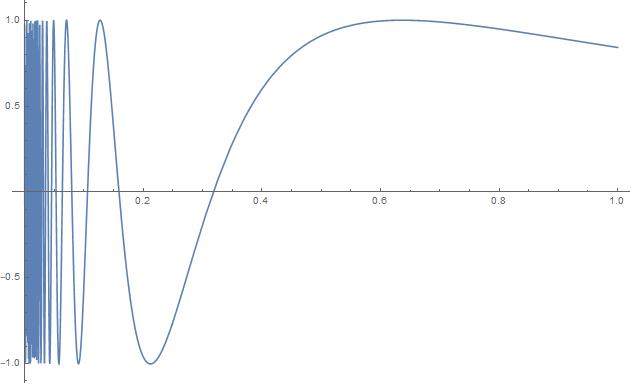
\includegraphics[scale=0.3]{Images/Top_sin.jpg}
    \caption{The topologists' sine curve}
    \label{tsine}
\end{figure}
The set is connected, since every point on the y-axis is a limit point of the curve. However, there is no continuous path connecting the y-axis to the rest of the curve, because $\sin(1/x)$ itself is not continuous.

\begin{xca}
\begin{enumerate}
    \item Show that the $n$-dimensional sphere $\bbS^n$ (defined as the unit sphere in $\bbR^{n+1}$ with the subset topology) is path-connected.
    \item Show that $\mathbb{Q}\subset\bbR $ is not connected.
    \item Show that the product of two path-connected spaces is path-connected.
\end{enumerate}
\end{xca}

\subsubsection{Compactness}

\begin{defn}[Covering/cover]
A collection of subsets of a topological space $X$ is said to cover $X$ if the union of these subsets equals $X$. If the subsets are all open (or closed), the covering (also often called a cover) is said to be open (resp.~closed).
\end{defn}

\begin{defn}[Compact Space]\index{Compact space}
A space $X$ is called compact if every open covering of $X$ contains a finite subcollection that also covers $X$ (\emph{subcovering}).
\end{defn}

\begin{defn}[Compact Subset]
A subset $A\subset X$ is called compact if it is compact in the subspace topology.
\end{defn}

\begin{prop}
If $Y_i\subset X$, $i = 1,\dots, m$ are compact subsets, then their union $\bigcup_{i=1}^m Y_i$ is also compact.
\end{prop}
\begin{proof}
Exercise.
\end{proof}

\begin{prop}[Compactness is a topological invariant]\label{prop f(compact)=compact}
The image $f(X)$ of a compact space $X$ under a continuous map $f\in C(X,Y)$ is compact.
\end{prop}
\begin{proof}
Exercise.
\end{proof}

\begin{xca}
\begin{enumerate}
    \item Show that the product of two connected spaces is connected. \emph{Hint:} first show that the union of any number of pairwise overlapping connected subspaces (i.e.\ subsets endowed with the subspace topology) of a space is also connected; then, write $X\times Y$ as the union of ``crosses'' $(\{x\}\times Y)\cup (X\times \{y\})$ that pairwise overlap and are connected only if $X$ and $Y$ are.
    \item Show that the product of two path-connected spaces is path-connected.
    \item Show that the product of two compact spaces is compact. \emph{Hint:} \cite{compact.proof}.
\end{enumerate}
\end{xca}


\begin{defn}[Classes of continuous maps]\index{Open map}\index{Closed map}\index{Proper map}
A map $f:X\to Y$ (not necessarily continuous) is called
\begin{enumerate}
    \item \emph{open} if the image of every open subset of $X$ is open in $Y$;
    \item \emph{closed} if the image of every closed subset of $X$ is closed in $Y$;
    \item \emph{proper} if it is continuous and the pre-image of any compact subset of $Y$ is compact in $X$;
\end{enumerate}
\end{defn}

\begin{xca}
   Show that the image of any proper map $f:\bbR^m\to\bbR^n$ is closed.
\end{xca}

\subsection{Metric spaces}

\begin{defn}[Metric spaces]\index{Metric space}\index{Metric}
A \emph{metric space} is a set $X$ with a \emph{metric} $\rho:X\times X\rightarrow \bbR $ that obeys the following conditions for any $x,y,z\in X$
\begin{enumerate}
    \item \emph{Non-negativity}: $\rho(x,y)\ge 0$; \emph{non-degeneracy:} $\rho(x,y)=0$ iff $x=y$.
    \item \emph{Symmetry}: $\rho(x,y) = \rho(y,x)$.
    \item \emph{Triangle Inequality}: $\rho(x,y) + \rho(y,z) \ge \rho(x,z)$.
\end{enumerate}
\end{defn}

\begin{defn}[Metric maps]
A \emph{metric map} between two metric spaces $(X,\rho_X)$ and $(Y,\rho_Y)$ is a continuous map $f\in C(X,Y)$ such that $\rho_Y (f(x_1),f(x_2))\leq \rho_X (x_1,x_2)$. The category $\mathsf{Met}$ is defined as the category of metric spaces with metric maps for morphisms.
\end{defn}

\begin{defn}[Open Ball]
An \emph{open ball} $B_r(x)$ of radius $r$ around a point $x$ in a metric space $(X,\rho)$ is defined as
\begin{equation}
    B_r(x) = \{ y\in X ~|~ \rho(y,x)< r \}
\end{equation}
\end{defn}

\begin{defn}[Metric Topology]
The metric topology induced by a metric on a set is the topology generated by basis elements that are open balls $B_r(x)$ for all $x\in X$ and $r>0$. 
\end{defn}
\begin{rem}
Equivalently, by Proposition \ref{characterization of topology using basis}, a set $M$ is open in the metric topology iff for any $x\in M$ there exists a radius $r>0$ such that $B_r(x)\subset M$. In the metric topology, $\rho:X\times X\to \mathbb R$ is automatically continuous.
\end{rem}
\begin{prop}
If a metric space $(X,\rho)$ is separable, it has a countable base.
\end{prop}
\begin{proof}
Exercise. \emph{Hint}: consider balls of rational radius about every point of the dense subset.
\end{proof}

\begin{defn}[Limit of a Sequence]
A sequence of points $\{x_n\}$ in a metric space $X$ is said to \emph{converge} if there exists a point $x\in X$ such that for any $\epsilon >0$, there exists an $N\in \mathbb{N}$ such that
\begin{equation}
    \forall ~ n>N,\; \rho(x_n,x) < \epsilon.
\end{equation}
The point $x$ is called the limit of the sequence.
\end{defn}
Note that the limit of a sequence is unique by the first axiom of the metric. One can also define the limit point of a subset of a general topological space as follows:
\begin{defn}[Limit Point]
If $A$ is a subset of a topological space, a point $x\in X$ is said to be a limit point of $A$ if every open neighbourhood of $x$ intersects $A$ in some point other than $x$.
\end{defn}

In metric spaces, limit points are equivalent to limits of sequences, i.e., for every limit point $x$ of a subset $A$, there exists a sequence of points in $A$ that converges to $x$. Conversely, for any convergent sequence of points in $A$, the limit of the sequence is a limit point of $A$.

\begin{prop}
For a metric space $X$ equipped with the metric topology, the closure $\xoverline{A}$ of a subset $A\subset X$ is equal to the set of limit points of $A$.
\end{prop}
\begin{proof}
Exercise.
\end{proof}

\begin{prop}
For two metric spaces $(X,\rho)$ and $(Y,\rho')$ and a map $f:X\rightarrow Y$ such that $f(x)=y$, the following are equivalent
\begin{enumerate}
    \item $f$ is continuous at $x$.
    \item For any convergent sequence $x_n\rightarrow x$, the image is also convergent with $f(x_n)\rightarrow y$.
    \item For every $\epsilon>0$, there exists $\delta>0$ such that $\rho(x,z)<\delta \implies \rho'(f(x)=y, f(z))<\epsilon$.
\end{enumerate}
\end{prop}
\begin{proof}
Exercise.
\end{proof}

\begin{defn}[Isometry]\index{Isometry}
An isometry between two metric spaces is a bijective map $f:X\rightarrow Y$ that preserves distances, i.e.,
\begin{equation}
    \rho_X(x,y) = \rho_Y(f(x), f(y)).
\end{equation}
\end{defn}

\begin{prop}
If $f:X\rightarrow Y$ is an isometry, it is also a homeomorphism.
\end{prop}
\begin{proof}
Exercise.
\end{proof}

\begin{defn}[Equivalent metrics]\index{Metric!equivalence of}
Two metrics $\rho_1,\rho_2$ on a topological space $X$ are called equivalent if for any $x\in X$ and any $r>0$, there exist radii $r',r''>0$ such that $B^{(1)}_{r'}(x)\subset B^{(2)}_{r}(x)$ and $B^{(2)}_{r''}(x)\subset B^{(1)}_{r}(x)$ (here, $B^{(i)}$ denotes an open ball defined by the metric $\rho_i$).
\end{defn}

\begin{thm}
Two metrics on the same space are equivalent iff they induce the same topology.
\end{thm}
\begin{proof}
Exercise.
\end{proof}

\begin{defn}[Cauchy sequence]\index{Cauchy sequence}
A sequence $(x_n)$ of points of a metric space $(X,\rho)$ is called a Cauchy sequence if for any $\epsilon>0$ there exists $N\in\mathbb{N}$ such that $\forall n,m\geq N$, $\rho(x_n,x_m)<\epsilon$.
\end{defn}

\begin{prop}
    A metric space is compact iff every sequence in it has a convergent subsequence (i.e.~it is \emph{sequentially compact}).
\end{prop}

\begin{defn}[Completeness]\index{Complete metric space}
A metric space $(X,\rho)$ is called complete if every Cauchy sequence $(x_n)$ in it has a limit $x_\infty\in X$.
\end{defn}


\begin{thm}[Cantor's intersection theorem]\index{Theorem!Cantor's intersection}
Let $(X,\rho)$ be a complete metric space and let $C_n$ be a sequence of closed nested subsets $C_{n+1}\subset C_n$ whose diameters tend to zero, $\mathrm{diam}\,C_n=\sup_{x,y\in C_n} \rho(x,y) \to 0$. Then the intersection $\bigcap_{n=1}^\infty C_n$ consists of exactly one point.
\end{thm}


\begin{prop}
    A metric space is sequentially compact iff every decreasing sequence of closed nonempty subsets (not necessarily tending to zero diameter) has a nonempty intersection.
\end{prop}


\begin{thm}
    A metric space is compact iff it is complete and for every $\epsilon>0$ it can be covered by a finite number of open balls of radius $\epsilon$ (i.e.~it is \emph{totally bounded}).
\end{thm}


\begin{xca}
Consider $\mathbb{N}$ with the metric $\rho (n,m)=\lvert \frac 1 n-\frac 1 m\rvert$. Construct a sequence of balls $B_{r_k}(x_k)$ in this space such that $r_{k+1}<r_k$, $B_{r_{k+1}}(x_{k+1})\subset B_{r_k}(x_k)$, but the intersection of all these balls is empty.
\end{xca}
\begin{defn}[Normed vector space]\index{Normed vector space}\index{Norm}
A normed vector space is a vector space $V$ over a subfield of $\mathbb{C}$ with a function (called the norm) $\lVert \cdot \rVert: V\to \mathbb R_+$ such that for all $x,y\in V$:
\begin{enumerate}
    \item $\lVert x\rVert\geq 0$, and $\lVert x\rVert= 0$ iff $x=0$;
    \item $\lVert \alpha  x\rVert=\lvert \alpha \rvert \lVert x\rVert$ for any scalar (element of the structure field) $\alpha$;
    \item $\lVert x+y\rVert\leq \lVert x\rVert+\lVert y\rVert$.
\end{enumerate}
Every normed vector space has a naturally induced metric $\rho (x,y)=\lVert x-y\rVert$. In the corresponding induced topology, the norm is automatically continuous.

\end{defn}
\begin{defn}[Equivalent norms]\index{Norm!equivalence of}
Two norms $\lVert\cdot \rVert_1,\lVert\cdot \rVert_2 $ on a vector space $X$ are called equivalent if there are (universal) constants $\alpha,\beta >0$ such that for all $x\in X$ we have $\alpha \lVert x \rVert_1\leq \lVert x \rVert_2 \leq \beta \lVert x \rVert_1$.
\end{defn}
Notice how this condition is much stronger than just the equivalence of the induced metrics, since $\alpha$ and $\beta$ are required to be universal constants for all $x$.

\begin{thm}
Two norms on a vector space $X$ are equivalent iff they induce the same topology.
\end{thm}
\begin{proof}
Exercise.
\end{proof}

\subsection{Separation axioms} \label{Separation Axioms}

We saw that every metric space has a canonical topology associated with it. A natural question to ask is whether the converse is true. Given a topological space, when can we define a metric on it such that the topology coincides with the metric topology? Clearly, a metric space has more structure than a topological space. In order to add more structure to topological spaces, we define the following axioms

\begin{defn}[Separation Axioms]\index{Separation axioms}
For a topological space $X$ with arbitrary points $x$ and $y$ and arbitrary disjoint closed sets $F$ and $G$, we define the following axioms:
\begin{enumerate}
    \item $T_1$: There exists an open neighbourhood $U$ of $x$ that doesn't include $y$, and an open neighbourhood $V$ of $y$ that doesn't include $x$, i.e., $x$ and $y$ are \emph{separated}.
    \item $T_2$ (\emph{Hausdorff}): There exist disjoint open neighbourhoods $U$ of $x$ and $V$ of $y$, i.e., $x$ and $y$ are \emph{separated by neighbourhoods}.
    \item $T_3$: There exist disjoint open neighbourhoods $U$ of $x$ and $V$ of $F$.
    \item \emph{Regular}: $X$ is both $T_1$ and $T_3$.
    \item $T_4$: There exist disjoint open neighbourhoods $U$ of $F$ and $V$ of $G$.
    \item \emph{Normal}: $X$ is both $T_1$ and $T_4$.
\end{enumerate}
\end{defn}

\begin{prop}
The following results demonstrate how each axiom adds additional structure to the space:
\begin{enumerate}
    \item $T_1 \implies$ All finite sets are closed;
    \item $T_2\implies T_1$;
    \item Regular $\implies$ Hausdorff;
    \item Normal $\implies$ Regular.
\end{enumerate}
\end{prop}

\begin{example}
The category $\mathsf{Hausd}$ of Hausdorff spaces is a full subcategory of $\mathsf{Top}$.
\end{example}

\begin{thm}[Urysohn Lemma]\index{Lemma!Urysohn}
A space $X$ is normal iff for any two disjoint closed subsets $A$ and $B$ there exists a continuous function
\begin{equation}
f\in C(X,[0,1]) ~\text{such that}~ \restr{f}{A} = 0, \restr{f}{B} = 1.
\end{equation}
\end{thm}

\begin{thm}
All metric spaces are normal.
\end{thm}
\begin{proof}
Exercise.
\end{proof}

\begin{thm}[Urysohn]
A normal space with a countable base is \emph{metrizable}, i.e., we can construct a canonical metric whose induced topology coincides with the topology of the space.
\end{thm}

\begin{prop}
If $X$ is Hausdorff, every compact subset of $X$ is closed.
\end{prop}
\begin{proof}
Exercise. \emph{Hint:} prove that the complement of the compact set is open by using Proposition \ref{open iff contains neighborhoods}.
\end{proof}

\begin{prop}
Every compact Hausdorff space is normal.
\end{prop}
\begin{proof}
Exercise.
\end{proof}

\begin{thm}[Heyne-Borel]\index{Theorem!Heyne-Borel}
In Euclidean space $\bbR^n$, a subset is compact iff it is closed and bounded.
\end{thm}

The following theorem is one of the most fundamental theorems in functional analysis, and it essentially characterizes compact subsets of the set of continuous functions defined on a compact subset of $\bbR^n$. We state it simply as an example of usage of the above topological terminology.
\begin{thm}[Arzel\`a-Ascoli]\index{Theorem!Arzel\`a-Ascoli}
Let $X$ be a compact Hausdorff space. A subset $F$ of the space $C(X,\bbR )$ of continuous real-valued functions on $X$ is relatively compact (i.e.\ its closure is compact) in the topology given by the sup-norm $\lVert f\rVert=\sup_X \vert f\rvert$ iff it is equicontinuous (i.e.\ all elements $f\in F$ are uniformly continuous functions and the $\delta$ in the definition of uniform continuity is universal for all $f\in F$) and pointwise bounded (i.e.\ for every $x\in X$ the set $\{f(x)\}_{f\in F}$ is bounded).
\end{thm}

\subsection{Homotopy}\label{sec.homotopy}
\begin{defn}[Homotopic maps]\index{Homotopy} Two continuous maps $f_0,f_1\in C(X, Y)$ are called homotopic (we often write $f\sim g$) if there exists a continuous map, called homotopy, $F\in C([0,1]\times X,Y)$ such that $F(0,x)=f_0(x)$ and $F(1,x)=f_1(x)$. Here, $[0,1]$ has the standard topology. For convenience, we will often describe homotopies as \emph{families of maps} $f_t:X\to Y$ defined by $f_t(x)=f(t,x)$.
\end{defn}
\begin{prop}
Homotopy is an equivalence relation on $C(X,Y)$. (The set of all homotopy classes of continuous maps from $X$ to $Y$ is denoted by $[X,Y]$. This set defines the morphisms in the (naive) homotopy category $\mathsf{hTop}$.)
\end{prop}
\begin{proof}
Exercise.
\end{proof}

The first argument of $F(t,x)$ is essentially ``time'', and $F(t,\cdot)$ continuously interpolates between $f_0$ and $f_1$ as time goes from 0 to 1. In topology, homotopy is synonymous with the phrase ``continuous deformation''.


\begin{defn}[Contractible space]\index{Contractible space}
A space $X$ is called contractible if it is homotopy equivalent to the one-point space, i.e.\ there exists a point $x_0\in X$ such that the constant map $f(x)=x_0$ is homotopic to the identity, $f\sim \id_X$. This property is in fact independent of $x_0$.
\end{defn}
\begin{prop}
Any contractible space is path-connected.
\end{prop}
\begin{proof}
Exercise. \emph{Hint:} consider paths traced out by $F(t,x)$ for fixed $x$'s.
\end{proof}
\begin{example}
\begin{enumerate}
    \item $\bbR^n$, $B^n$, $(0,1)^n$ are all contractible via, say, $F(t,x)=tx$ (they are also all homeomorphic to each other).
    \item Any two continuous functions $f,g:\bbR \to\bbR $ are homotopic via homotopy $F(t,x)=tg(x)+(1-t)f(x)$.
\end{enumerate}
\end{example}
\begin{xca}
Show that if $Y$ is contractible, then any two maps $f,g\in C(X,Y)$ are homotopic. This is a generalization of the above example for $X=Y=\bbR $.
\end{xca}
\begin{thm}[Brouwer]
The sphere $\bbS^n$ is not contractible.
\end{thm}
\begin{proof}
    There is a plethora of different ways to prove this theorem, from pure analytical to algebraic. We will delay the proof until we compute the homology groups of the spheres in Part \ref{Part II} and observe that they differ from those of a contractible space (and homology groups are topological invariants).
\end{proof}
\begin{thm}[Brouwer's fixed point theorem]\index{Theorem!Brouwer's fixed point}\label{thm Brouwer's fixed point}
Any continuous map $f\in C\left(\xoverline{B^n},\xoverline{B^n}\right)$  from the closed unit ball to itself has at least one fixed point ($x_0$ such that $f(x_0)=x_0$).
\end{thm}
\begin{proof}
For $n=1$ this is clear. For $n\geq 2$, suppose $f(x)\neq x$ for all $x$. Then we can define $h(x)$ as the point of intersection of the ray $[f(x),x)$ with the boundary of the ball. Then $F(t,x)=h(tx)$ is a contracting homotopy, which contradicts the last theorem.
\end{proof}
\begin{rem}
These two theorems are in fact equivalent. The fixed point theorem can be proven purely analytically, and the contractibility theorem will follow. The simplest modern proof of non-contractibility of $\bbS^n$ is based on homology.
\end{rem}

\begin{defn}[Retraction, Deformation retraction]\index{Retraction}\index{Deformation!retraction}
    A retraction of a topological space $X$ onto its subspace $A\subset X$ is a continuous map $r:X\to A$ such that $\restr{r}{A}=\mathrm{id}_A$. A deformation retraction is a homotopy from the identity map $\mathrm{id}_X$ to $r$. A \emph{strong} deformation retraction also satisfies $\restr{r_t}{A}=\mathrm{id}_A$ for all $t\in[0,1]$ (this is often included in the definition of a deformation retraction).
\end{defn}

\begin{defn}[Homotopy equivalence of spaces]\index{Homotopy equivalence}
Two topological spaces $X$ and $Y$ are called homotopy equivalent if there exist two continuous maps $f\in C(X,Y)$, $g\in C(Y,X)$ such that their compositions are homotopic to identity: $g\circ f\sim \id_X$ and $f\circ g\sim \id_Y$. We write $X\simeq Y$.
In the presence of basepoints, these homotopies are required to leave the basepoints fixed for all values of the deformation parameter $t$.
\end{defn}

\begin{cor}
    \begin{enumerate}
        \item Deformation retractions are homotopy equivalences.
        \item Contractible spaces are homotopy equivalent to a point.
    \end{enumerate}
\end{cor}

\begin{example}
\begin{enumerate}
    \item $\bbS^1\times\bbR \simeq \bbS^1\simeq M$, where $M$ is the M\"obius band.
    \item $\bbR^n\setminus{0}\simeq \bbS^{n-1}$.
    \item More generally, two spaces $X,Y$ are homotopy equivalent iff they are both deformation retracts of the same space $Z$. That is, there needs to exist $A_X\subset Z$ such that $A_x\cong X$ and there exists a continuous map $F\in C([0,1]\times Z,Z)$ such that $F_X(0,z)=z$, $F_X(1,z)\in A$ and $F_X(t,a)=a$ for any $z\in Z$, $t\in [0,1]$ and $a\in A_x$. Similarly, there needs to exist $A_Y\subset Y$ homeomorphic to $Y$ that is a deformation retract of $Z$.
\end{enumerate}
\end{example}

\subsection{The fundamental group}

\begin{defn}[Loops, Pointed homotopy]\index{Loop}
Let $X$ be a path-connected topological space, pick a ``base point'' $x_0\in X$, and consider the set of all \emph{loops} in $X$ based at $x_0$, i.e.\ paths $\gamma\in C([0,1], X)$ such that $\gamma(0)=\gamma(1)=x_0$. A pointed homotopy between two such loops is a homotopy $F\in C([0,1]\times[0,1],X)$ such that $F(\cdot,0)=F(\cdot,1)=x_0$. Pointed homotopy is an equivalence relation on the set of based loops.
\end{defn}

\begin{defn}[Fundamental/Poincar\'e group]\index{Fundamental group}
The fundamental group $\pi_1(X,x_0)$ of a path-connected space $X$ with a base point $x_0$ is defined as the set $\{ [\gamma]\}$ of pointed homotopy classes of based loops with the inversion operation given by $[\gamma(t)]^{-1}=[\gamma(1-t)]$ and the multiplication operation 
\[
[\gamma_1(t)]\circ [\gamma_2(t)]=\left[ \begin{cases} \gamma_1(2t), & t\in[0,1/2], \\ \gamma_2(2t-1), & t\in(1/2,1] \end{cases}\right].\label{pi1 group op}
\]
The unit element is given by the equivalence class of the ``constant loop'' $\gamma(t)\equiv x_0$. If $X$ is not path-connected, then $\pi_1(X,x_0)$ is defined as the fundamental group of the path-connected component containing $x_0$.
\end{defn}

\begin{xca}
Check that this definition is consistent, i.e.\ the homotopy classes on the right-hand sides don't depend on the choices of representatives of the classes on the left.
\end{xca}
\begin{defn}[Simple-connectedness]\index{Simply connected space}
A path-connected space $X$ is called simply connected if its fundamental group is trivial, $\pi_1(X,x_0)=\{e\}$.
\end{defn}

\begin{xca}
Show that contractible spaces are simply connected.
\end{xca}

\begin{thm}
    If a space $X$ retracts onto a subspace $A$, then the homomorphism of fundamental groups $i_\ast:\pi_1(A,x_0)\to \pi_1(X,x_0)$ induced by the inclusion $i: A\hookrightarrow X$ is injective. If $A$ is a deformation retract of $X$, then $i_\ast$ is an isomorphism.
\end{thm}
\begin{proof}
    If $r:X\to A$ is a retraction then $r\circ i=\mathrm{id}_A$, hence by functoriality of $\pi_1$, $r_\ast \circ i_\ast=\mathrm{id}_{\pi_1(A,x_0)}$, which implies injectivity. If $r_t$ is a deformation retraction, then for any loop $\gamma$ in $X$ based at $x_0\in A$ the composition $r_t\circ \gamma$ gives a homotopy of $\gamma$ to a loop in $A$, therefore $i_\ast$ is also surjective.
\end{proof}

\begin{defn}[Alternative approach]
Recall that the category $\mathsf{Top}_\bullet$ consists of ``pointed topological spaces'' with chosen basepoints and morphisms that are continuous maps mapping basepoint to basepoint. Take the circle $\bbS^1$ and pick a point $\bullet$ in it. Then one can redefine based loops as morphisms between two pointed topological spaces $\gamma\in C((\bbS^1,\bullet),(X,x_0))$. Pointed homotopy in the definition of $\pi_1$ can then be replaced by just homotopy of loops as maps defined on $\bbS^1$.   Thus, as a set, $\pi_1(X)=[\bbS^1,X]_\bullet$ (group of homotopy classes of pointed maps).
\end{defn}

\begin{defn}[Suspension]\index{Suspension}
    The suspension of a topological space $X$, is defined as the quotient space $SX=(X\times [0,1])/(X\times \{0\},X\times\{1\})$ (i.e.\ a cylinder over $X$ where each of the two faces is then collapsed into a point -- best visualized as a double cone over $X$). If $X$ is a pointed space with basepoint $x_0$, then the \emph{reduced suspension} is defined as $\Sigma X=(X\times [0,1])/(X\times \{0\},X\times\{1\} ,\{x_0\}\times [0,1]))$, and the new basepoint is the image of $(x_0,0)$ in the quotient. Equivalently, $\Sigma X=X\wedge \bbS^1=X\times \bbS^1/(X\vee \bbS^1)$.
\end{defn}

\begin{xca}
    Verify that $\Sigma$ extends to a functor on the category of pointed spaces. This will follow from the uniqueness of the pointed map at the bottom of the following square that makes it commute:
    \[\begin{tikzcd}[every matrix/.append style={name=m},   
    execute at end picture={\draw [<-] ([xshift=-2.3em,yshift=1mm]m-2-2.north) arc[start angle=-90,delta angle=270,radius=0.25cm];}]
   X \arrow[r,"f"]\arrow[d,swap,"\pi_X"]& Y\arrow[d,"\pi_Y"] \\
   \Sigma X\arrow[r,swap,dashed, "\exists !\,\Sigma(f)"]& \Sigma Y
    \end{tikzcd}\]
    where $\pi_X$ and $\pi_Y$ are the quotient maps that define the suspensions.
\end{xca}

\begin{example}
    From Exercise~\ref{wedge sums} we have $\Sigma \bbS^n\cong \bbS^{n+1}$. This holds even when $n=0$ and $\bbS^0=\{-1,1\}$.
\end{example}

\begin{defn}[Compact-open topology]
    Given two spaces $X,Y$, denote the set of all continuous maps between them by $Y^X=C(X,Y)$. The compact-open topology on $Y^X$ is generated\tablefootnote{The topology generated by a collection of sets is simply the coarsest topology in which all of those sets are open. This topology consists of all unions and all finite intersections of these sets.} by the sets $M(K,U)=\{f\in Y^X\mid f(K)\subset U\}$ where $K\subset X$ is compact and $U\subset Y$ is open.
\end{defn}

\begin{prop}
    If $X,Y$ are Hausdorff and $X$ is locally compact, then $C(X,Y)$ is Hausdorff.
\end{prop}
\begin{proof}
    Let $f,g\in C(X,Y)$ with an $x\in X$ such that $f(x)\neq g(x)$. Since $Y$ is Hausdorff, there exist disjoint open neighborhoods $U_1$ of $f(x)$ and $U_2$ of $g(x)$. Then $f^{-1}(U_1)\cap g^{-1}(U_2)$ is an open neighborhood of $x$, because $f$ and $g$ are continuous. Since $X$ is locally compact, this neighborhood contains a compact neighborhood $K$. Then, $M(K,U_1)$ and $M(K,U_2)$ are neighborhoods of $f$ and $g$, respectively. They are disjoint because $U_1$ and $U_2$ are.
\end{proof}

\begin{prop}
    If $X$ is a locally compact Hausdorff space, then the evaluation map $e:Y^X\times X\to Y$, defined by $e(f,x)=f(x)$, is continuous.
\end{prop}
\begin{proof}
    Let $U$ be an open neighborhood of $f(x)$. Since $f$ is continuous and due to the properties of $X$, there is a compact neighborhood $K$ of $x$ such that $f(K)\subset U$. Thus $f\in M(K,U)$ and $M(K,U)\times K$ is mapped into $U$ by the evaluation map $e$. Finally, $M(K,U)\times K \subset Y^X\times X$ is a neighborhood of $(f,x)$. This proves continuity.
\end{proof}


\begin{thm}\label{compact open continuity}
    Let $X$ be a locally compact Hausdorff space, and $Y$ and $T$ Hausdorff spaces. For any map $f:X\times T\to Y$, denote $f_t(x)=f(x,t)$. Then the continuity of $f$ is equivalent to each $f_t$ being continuous separately and the mapping $t\mapsto f_t$ also being continuous from $T$ into $Y^X$. 
\end{thm}
\begin{proof}
    See \cite[Theorem VII.2.4]{Bredon}.
\end{proof}
This Theorem implies that if $X$ is locally compact, then a homotopy $X\times [0,1]\to Y$ is the same thing as a path $[0,1]\to Y^X$.
\begin{cor}[The Exponential Law]
    Let $X,T$ be locally compact Hausdorff spaces, and $Y$ a Hausdorff space. Then the bijection from Theorem \ref{compact open continuity} is a natural homeomorphism $Y^{X\times T}\cong \left(Y^X\right)^T$ taking $f$ to $f^\ast$ defined as $f^\ast (t)(x)=f(x,t)=f_t(x)$.
\end{cor}
\begin{proof}
    See \cite[Theorem VII.2.5]{Bredon}.
\end{proof}
Similarly, one can show that under similar conditions, one has homeomorphisms $Y^X\times W^X\cong (Y\times W)^X$ (under $f\times g$), $Y^{X\sqcup T}\cong Y^X\times Y^T$ (under $f\sqcup g$), and $Z^Y\times Y^X \cong Z^X$ (under $f\circ g$). For details see \cite[\S VII.2]{Bredon}.
\begin{defn}[Loop space]\index{Loop space}
    The loop space of a pointed space $X$ is the space $\Omega X=X^{\bbS^1}$ that consists of loops based at $x_0$, with the compact-open topology. Its basepoint is the constant loop at $x_0$.
\end{defn}


\begin{prop}\label{suspension maps prop}
    \begin{enumerate}
        \item The set of homotopy classes $[X;\Omega Y]$ is a group under the multiplication induced by the usual multiplication of loops in $Y$;
        \item The set of homotopy classes $[\Sigma X;Y]$ is a group under the multiplication induced by the concatenation of maps along the interval $[0,1]\times\{x_0\}$ in $\Sigma X$ (namely $f(2t,x)$ for $t\leq 1/2$ and $g(2t-1,x)$ after that);
        \item On the set $[\Sigma X;\Omega Y]$, the two multiplications defined above coincide and are abelian.
    \end{enumerate}
\end{prop}
\begin{proof}
    Item 1 is obvious and Item 2 is easily checked by verifying that the concatenation of a map with its time-reversed copy ($f(1-t,x)$) is homotopic to the constant map.

    In item 3, such maps can be denoted $f_{t,s}(x)$, where $t$ is the parameter in $\Sigma X$ and $s$ is the one in $\Omega Y$. The two multiplications differ only in which of these two parameters maps get concatenated along. The idea is then to homotopically deform one into the other. This can be done by using a deformation retract of the square $[0,1]^2$ into a smaller square in the center.  Since we're working with pointed spaces, the whole boundary of the square gets mapped to the basepoint $y_0$. Hence we can replace $f$ and $g$ with their retractions to the smaller square, whereas outside of that square the value is just $y_0$. Now the two different concatenations are clearly homotopic to each other since we can smoothly ``slide'' the domains of $f$ and $g$ around each other, and then undo the original deformation retract. This proves both the equality of the two products and their commutativity. See figure.
    \begin{center}
    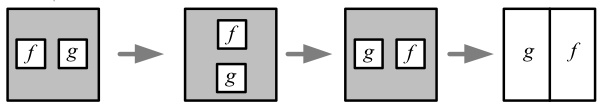
\includegraphics[scale=1]{Images/higher-homotopy.png}
    \end{center}
\end{proof}

\begin{lem}\label{lemma on suspension and loops}
    For any pair of pointed spaces $X,Y$, there is a natural isomorphism of groups $[\Sigma X,Y]\approx [X,\Omega Y]$.
\end{lem}
\begin{proof}
    The isomorphism is induced by the correspondence that identifies $f(t,x)$ with $\gamma(x)(t)=f(t,x)$. One can easily check that this provides a one-to-one correspondence between pointed maps and pointed homotopy on both sides. Furthermore, it is almost obvious that the multiplication on both sides works the same way.
\end{proof}

\begin{defn}[Zeroth degree homotopy set]
    Denote by $\pi_0(X)$ the set of path-connected components of $X$. It can be identified with the set of homotopy equivalence classes of maps from the one-point space into $X$. Note that this set carries no natural structure of a group.
\end{defn}

\begin{rem}
    One of the most useful consequences of the above discussion is that in sufficiently nice topological categories, such as that of topological manifolds, homotopies are just paths in the space of continuous maps. Therefore homotopy classes of maps $[X;Y]$ are nothing but the path-connected components in the space $Y^X$, that is, $\pi_0( Y^X)$. For compact $X$ Lemma~\ref{lemma on suspension and loops} can be shown indirectly using the exponential law, $Y^{\Sigma X}\cong (\Omega Y)^X$. As we've just seen, the multiplications on these spaces correspond, thus we have group homomorphisms $[\Sigma X;Y]= \pi_0(Y^{\Sigma X})\cong \pi_0((\Omega Y)^X)= [X;\Omega Y]$.
\end{rem}
\begin{prop}\label{prop computing pi1}
\begin{enumerate}
    \item $\pi_1$ is a covariant functor $\pi_1:\mathsf{Top}_\bullet\to \mathsf{Gr}$.
    \item For a path-connected space, fundamental groups with different base points are isomorphic (this is why we often abuse the notation by writing $\pi_1(X)$).
    \item For any number of path-connected spaces, $\pi_n(\prod_\alpha X_\alpha)\cong \prod_\alpha \pi_n(X_\alpha)$.
\end{enumerate}
\end{prop}
\begin{proof}
Exercise.
\end{proof}

\begin{lem}\label{lem product of loops}
    If a space $X$ is the union of a collection of path-connected open sets $U_\alpha$ each containing the basepoint $x_0$ and if each intersection $U_{\alpha\beta}$ is path-connected, then every loop in $X$ at $x_0$ is homotopic to a product of loops each of which is contained in a single $U_\alpha$.
\end{lem}
\begin{proof}
    The key is in the compactness of the interval $[0,1]$, which guarantees that the loop can be broken up into a finite number segments each of whose closure is contained inside only one of the $U_\alpha$'s. Call these segments $f_i, i=1,\ldots,n$. Since $x_0$ belongs to each $U_\alpha$, we can then find a path $g_i$ from $x_0$ to the starting point of $f_i$. We can always choose $g_0$ and $g_{n+1}$ to be trivial. The loops we seek are then $g_i\cdot f_i\cdot g_{i+1}^{-1}$. Their product is homotopic to the original loop because all $g_i$'s cancel out.
\end{proof}
\begin{cor}\label{cor pi_1(S^n)=0}
    $\pi_1(\bbS^n)=0$ for $n\geq 2$.
\end{cor}
\begin{proof}
    $\bbS^n$ is the union of the open neighborhoods of two hemispheres, $U_+$ and $U_-$. Each of these is homeomorphic to $\bbR^n$ and $U_+\cap U_-\cong \bbS^{n-1}\times \bbR $. If $n\geq 2$, then $U_+\cap U_-$ is path-connected. By the above lemma, every loop in $\bbS^n$ based at a point $x_0\in U_+\cap U_-$ is a product of two loops within each hemisphere. However both of these loops are trivial since $\pi_1(U_\pm)=0$.
\end{proof}
\begin{cor}
    $\bbR^2$ is not homeomorphic to $\bbR^n$ for $n\neq 2$.
\end{cor}
\begin{proof}
    Assume there is a homeomorphism $f:\bbR^2\to \bbR^n$. The case $n=1$ is easy because $\bbR \setminus\{f(0)\}$ is not connected whereas the supposedly homeomorphic $\bbR^2\setminus\{0\}$ is. 
    When $n>2$, the complement $\bbR^n\setminus\{f(x)\}$ is homeomorphic to $\bbS^{n-1}\times \bbR $, whose fundamental group is $\pi_1(\bbS^{n-1})=0$ by Proposition~\ref{prop computing pi1}. However, for $n>2$ the fundamental group of the complement $\bbR^2\setminus\{x\}$ is $\pi_1(\bbS^1)=\bbZ$. This leads to a contradiction.
\end{proof}

We are now prepared to prove one of the most important theorems about the fundamental group. First let us recall the categorical notion of pushouts (see Definition~\ref{pushouts}). If a path-connected space is represented as a union of two open sets, $X=U\cup V$, then the corresponding set inclusions induce homomorphisms of fundamental groups:
\[
\begin{tikzcd}[every matrix/.append style={name=m},   
execute at end picture={\draw [<-] ([xshift=-8.5mm,yshift=1mm]m-2-2.north) arc[start angle=-90,delta angle=270,radius=0.25cm];}]
   X \arrow[r,leftarrow,"l"]\arrow[d,leftarrow,"k"]& V\arrow[d,leftarrow,"j"] \\
   U\arrow[r,,leftarrow,swap,"i"]& U\cap V\\
\end{tikzcd}
\quad\quad\quad\quad\quad
\begin{tikzcd}[every matrix/.append style={name=m},   
execute at end picture={\draw [<-] ([xshift=-11.5mm,yshift=1mm]m-2-2.north) arc[start angle=-90,delta angle=270,radius=0.25cm];}]
   \pi_1(X) \arrow[r,leftarrow,"l_\ast"]\arrow[d,leftarrow,"k_\ast"]& \pi_1(V)\arrow[d,leftarrow,"j_\ast"] \\
   \pi_1(U)\arrow[r,,leftarrow,swap,"i_\ast"]& \pi_1(U\cap V)\\
\end{tikzcd}
\]
$X$ itself is in fact the pushout, $X=U\sqcup_{U\cap V}V$. \emph{The Siefert-van~Kampen theorem will show that the functor $\pi_1$ preserves pushouts,} i.e.\ the fundamental group of the union is isomorphic to the amalgamated free product, $\pi_1(X)\cong \pi_1(U) \ast_{\pi_1(U\cap V)} \pi_1(V)$. By the universal property of the free product, there is a unique homomorphism $\Phi$ in the diagram below that makes the external triangles commute.
\[
\begin{tikzcd}
  \pi_1(U)\ast \pi_1(V)   \arrow[drr,leftarrow, bend left]   \arrow[ddr,leftarrow, bend right]   \arrow[dr,"\exists! \Phi" description] & & \\
    & \pi_1(X) \arrow[r,leftarrow,swap, "l_\ast"] \arrow[d,leftarrow, "k_\ast"]       & \pi_1(V) \arrow[d,leftarrow, "j_\ast"] \\ & \pi_1(U) \arrow[r,leftarrow,swap, "i_\ast"] &\pi_1(U\cap V) 
\end{tikzcd}
\]
Note, however, that the ``background square'' involving $\pi_1(U\cap V),\pi_1(U),\pi_1(V)$, and $\pi_1(U)\ast \pi_1(V)$ \emph{does not commute}, so the universal property of the pushout \emph{will not} apply in the other direction to give a homomorphism $\pi_1(X)\to \pi_1(U)\ast\pi_1(V)$. Instead, we will compute $\pi_1(X)$ by finding the kernel of $\Phi$ and factoring it out.

\begin{thm}[Siefert-van Kampen]\index{Theorem!Siefert-van~Kampen}
    If $X$ is the union of path-connected open sets $U_\alpha$ each containing the basepoint $x_0\in X$ and if each intersection $U_{\alpha\beta}$ is path-connected, then the homomorphism $\Phi: \ast_\alpha \pi_1(U_\alpha)\to \pi_1(X)$ induced by the inclusions $U_\alpha \hookrightarrow X$ is surjective. 
    
    Denote the inclusion-induced homomorphisms $i_\alpha:\pi_1(U_\alpha)\to \pi_1(X)$ and $i_{\alpha\beta}:\pi_1(U_{\alpha\beta})\to \pi_1(U_\alpha)$. We have $i_\alpha \circ i_{\alpha\beta}=i_{\beta}\circ i_{\beta\alpha}$ since both sides are induced by the inclusion $U_{\alpha\beta}\hookrightarrow X$. Now, if in addition each intersection $U_{\alpha\beta\gamma}$ is path-connected, then the kernel of $\Phi$ is the normal subgroup $N$ generated by all elements of the form $i_{\alpha\beta }(g)i_{\beta\alpha}(g)^{-1}$ for $g\in\pi_1(U_{\alpha\beta})$, and hence $\Phi$ induces a homomorphism $\pi_1(X)\cong \ast_\alpha \pi_1(U_\alpha)/N$.

    In particular, in the case of two sets, $\pi_1(U\cup V)\cong \pi_1(U)\ast_{\pi_1(U\cap V)}\pi_1(V)$.
\end{thm}
\begin{proof}
    The surjectivity of $\Phi$ was already shown in Lemma~\ref{lem product of loops}. 
    
    Now we need to show that the kernel of $\Phi$ is exactly $N$. We already know that $N\subset \ker \Phi$ since $i_\alpha\circ i_{\alpha\beta}=i_\beta\circ i_{\beta\alpha}$. For the reverse inclusion, the idea is to study \emph{factorizations} of loops into ``smaller'' loops $[\gamma_i]$ that are completely contained in one of the $U_\alpha$'s. There are two ``moves'' that, as we would like to show, transform differing factorizations of the same loop into each other. Namely, a substring of the form $[\gamma_i][\gamma_{i+1}]$ can be replaced with $[\gamma_i\cdot \gamma_{i+1}]$, and an element $[\gamma_i]$ viewed as an element of $\pi_1(U_\alpha)$ can be replaced with its analog in $\pi_1(U_\beta)$ if $\gamma_i$ is a loop contained in $U_{\alpha\beta}$. If we can show that all factorizations of a loop can be transformed into each other via a sequence of moves of this kind (or their inverses), that will mean that $\Phi$ induces an \emph{injective} map from the quotient group into $\pi_1(X)$, and thus the kernel of $\Phi$ is exactly $N$.

    The goal is therefore to decompose any homotopy of loops into a sequence of moves like this. A homotopy is a continuous map defined on the unit square, $H:[0,1]\times[0,1]\to X$, whose value on the left and right edges of the square is $x_0$. Now we need to subdivide this square into smaller squares as in the Figure, so that each square is mapped entirely into only one of the open sets $U_\alpha$, and so that the resulting subdivisions of the top and bottom edges of the square are refinements of the subdivisions implied in the two factorizations at hand (that is, each interval of the new subdivision is entirely contained in an interval from the old). Lastly, we can ``perturb'' the squares in the central rows so that each point is contained in at most three squares (this is why triple intersections were required to be path-connected).

    \begin{center}
        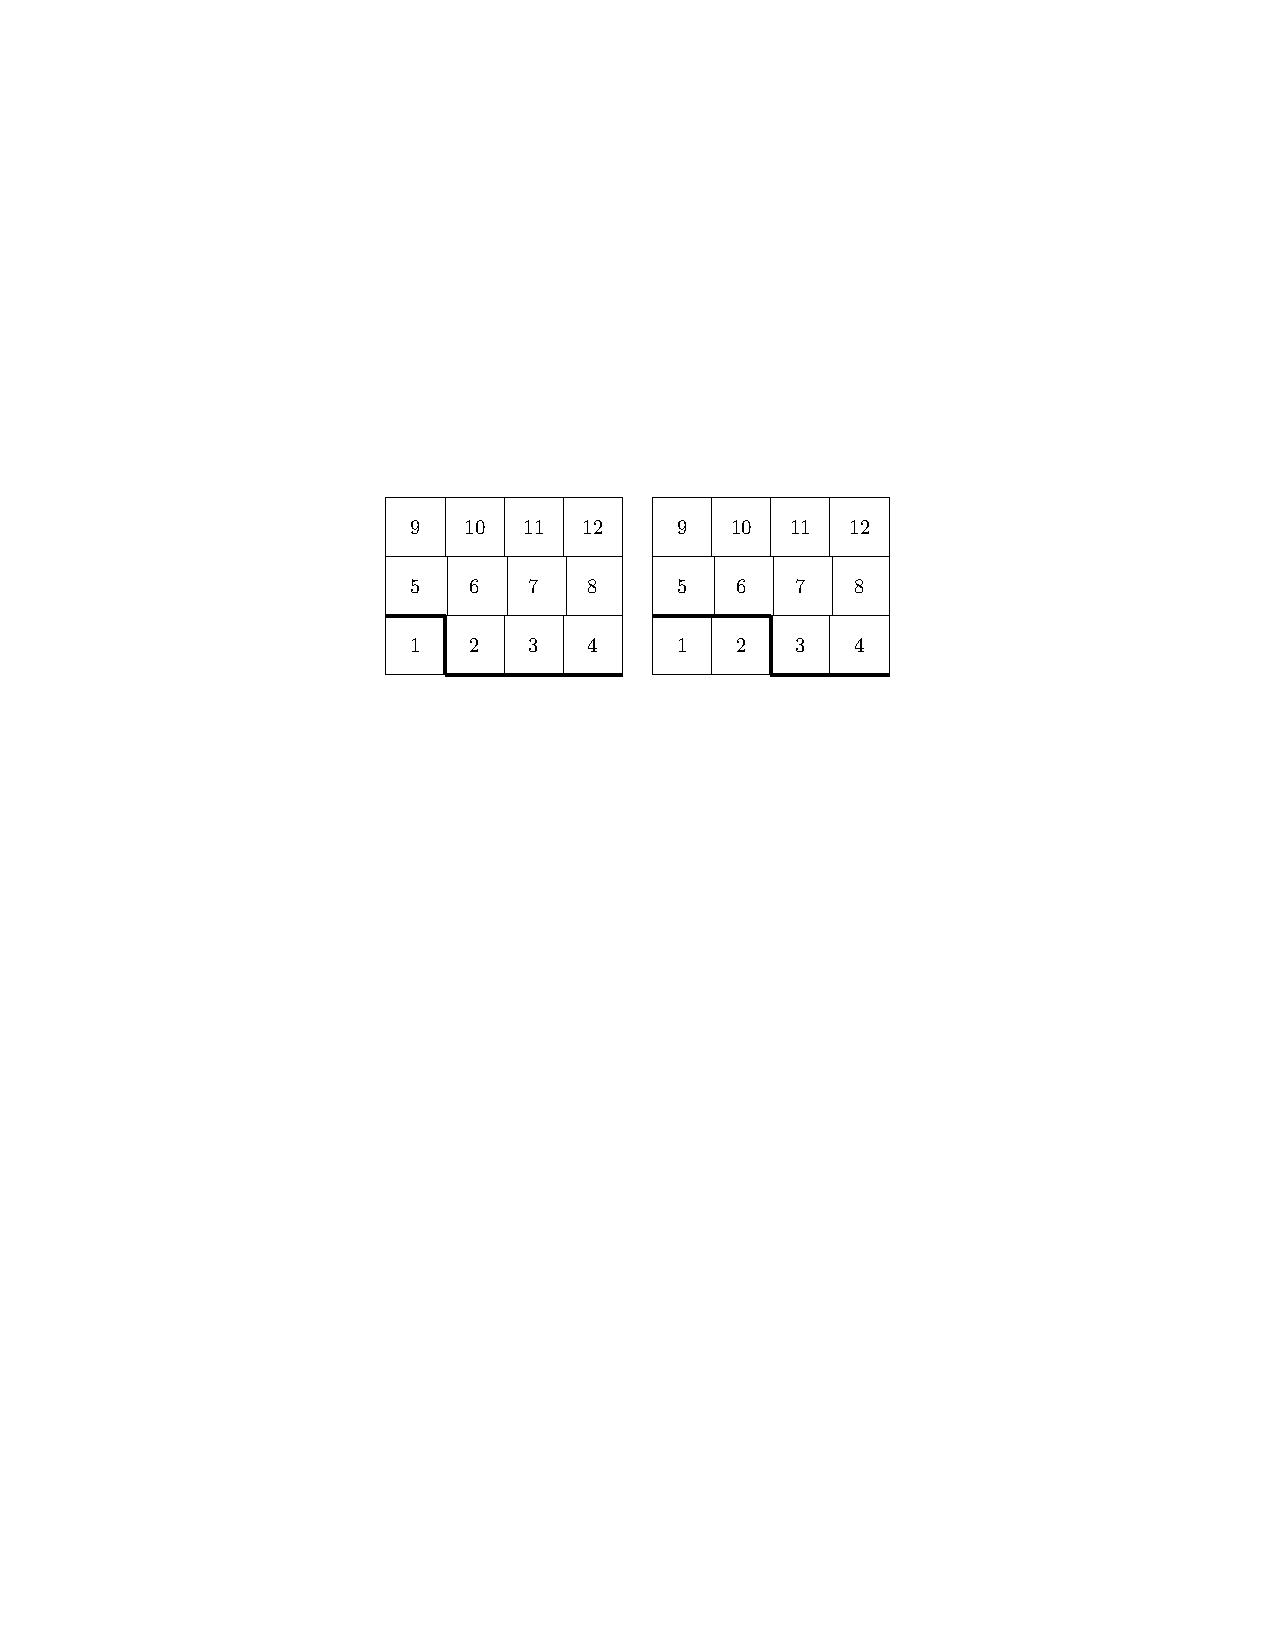
\includegraphics[scale=1]{Images/subdivision.pdf}
    \end{center}

    Now we proceed to define a sequence of paths along the edges of the subdivision from the left to the right side of the square that progressively ``capture'' more and more of the squares. For each segment we need to specify which of the open sets in $X$ its image is supposed to belong to, which is exactly the second move (in other words, $i_{\alpha\beta\ast}([\gamma_i])$ and $i_{\beta\alpha\ast}([\gamma_i])$ belong to the same coset in the quotient group). Further, each successive path is homotopic to the last via a deformation of a loop inside one $U_\alpha$. All together, this proves that any two factorizations of the same loop are equivalent in the sense that they differ only by relations that define the group $N$. The illustration below is from \cite[Chapter 10]{LeeTop}.

    \begin{center}
        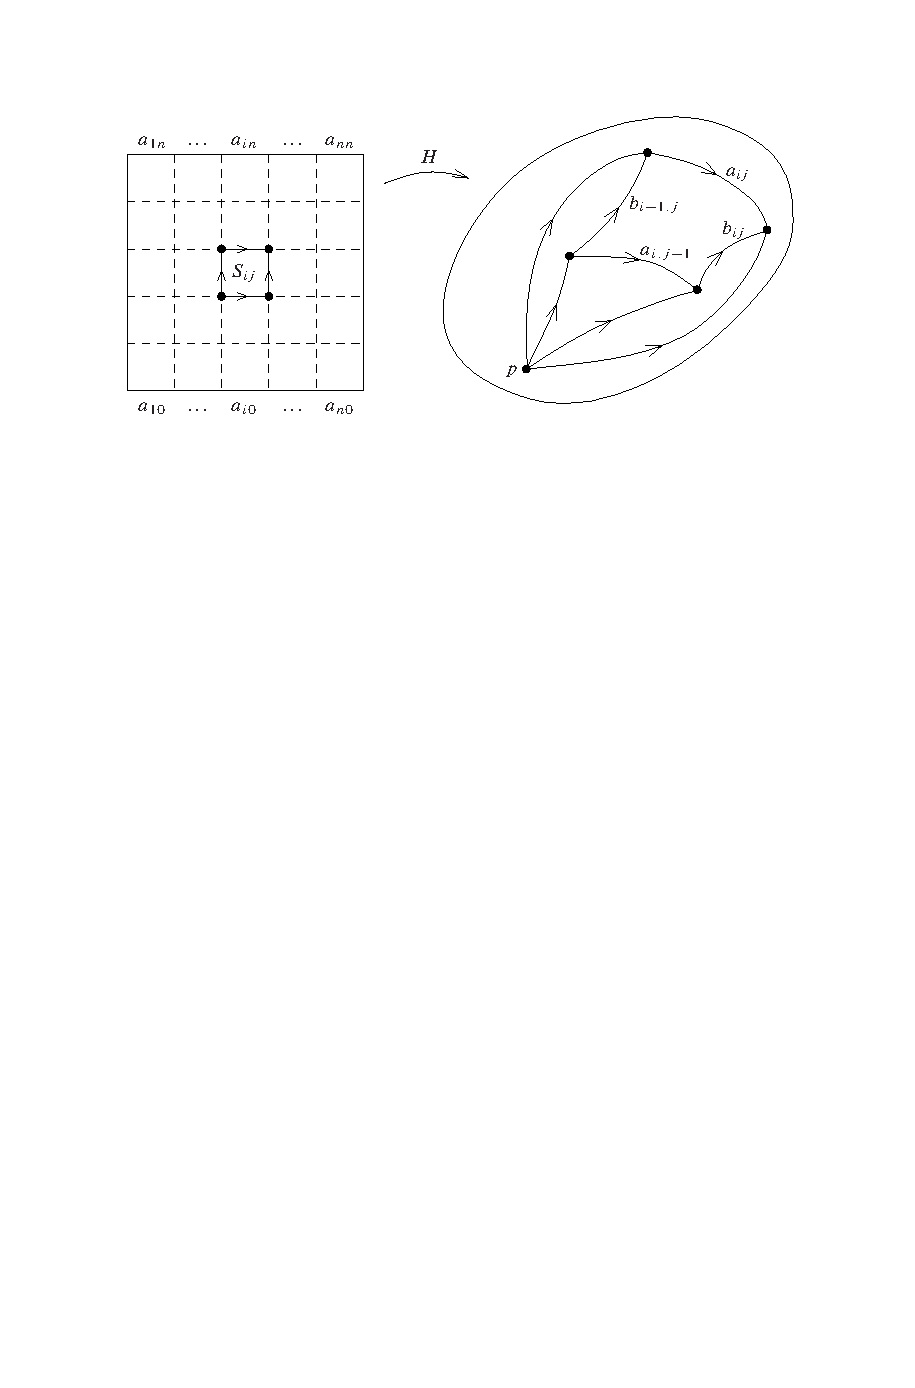
\includegraphics[scale=1]{Images/kernel of Phi.pdf}
    \end{center}
    
    See \cite[Theorem 1.20]{Hatcher} for more details of the proof.
\end{proof}

The conditions on path-connectedness of intersections and on the basepoint seem artificial, and indeed the are. Any open covering of $X$ can be turned into a cover of this kind by taking unions of sets lying along paths connecting them to the original basepoint. The full version of the Seifert-van~Kampen theorem can be stated purely in categorical terms with no extra conditions, however first we will need the notion of the \emph{fundamental groupoid}.

\begin{defn}[Groupoid]\index{Groupoid}
    A groupoid is a set with a unary ``inversion'' map $x\mapsto x^{-1}$ and a partial (i.e.\ not necessarily defined for any pair of elements) associative binary ``multiplication'' operation $(x,y)\mapsto x\bullet y$. It is associative in the sense that if both $x\bullet y$ and $y\bullet z$ exist, then both $(x\bullet y)\bullet z$ and $x\bullet (y\bullet z)$ exist and coincide. It is also required that $x\bullet x^{-1}$ and $x^{-1}\bullet x$ exist, and that, if $x\bullet y$ exists, then $x\bullet y\bullet y^{-1}=x$ and $x^{-1}\bullet x\bullet y=y$.

   As a consequence of these axioms, $(x^{-1})^{-1}=x$ and $(x\bullet y)^{-1}=y^{-1}\bullet x^{-1}$. Intuitively, groupoids can be thought of as groups with many identities, where only elements belonging to the same identity (which is the case if $x\bullet x^{-1}=x\bullet x^{-1}$) can be multiplied. 
    
    An equivalent definition is that a groupoid is a category where all morphisms are invertible (i.e.\ isomorphisms). The objects of this category are the ``identities'' of the groupoid. A group is then simply a groupoid with a single object. The category of groupoids is denoted $\mathsf{Grpd}$.
\end{defn}

Free products of groupoids can be constructed in the same way as for groups -- as strings of ``words'' $g_1^{\epsilon_1} \cdots g_n^{\epsilon_n}$ where each product $g_i^{\epsilon_i}\bullet g_{i+1}^{\epsilon_{i+1}}$ must exist and insertions of substrings of the form $gg^{-1}$ produce an equivalent string. These free products have the same universal property and are therefore the pushouts in $\mathsf{Grpd}$.

\begin{defn}[Fundamental groupoid]\index{Fundamental groupoid}
    Given a topological space $X$, let $\Pi(X)$ (also denoted $\Pi_1(X)$) be the category whose objects are points of $X$ and the morphisms $\mathrm{Mor}(x,y)$ are the homotopy equivalence classes of paths $\gamma:[0,1]\to X$ such that $\gamma(0)=x, \gamma(1)=y$. Since continuous images of homotopic paths are homotopic, we have a functor $\Pi:\mathsf{Top}\to \mathsf{Grpd}$.
\end{defn}
Notice that the set of endomorphisms of any $x\in X$ viewed as an object in $\Pi(X)$ is exactly the group $\pi_1(X,x)$. Moreover, it's not difficult to check that homotopies of continuous maps in $\mathsf{Top}$ induce natural transformations of the corresponding $\Pi$-functors.
\begin{prop}
    For a path-connected space $X$, the inclusion $\pi_1(X,x)\hookrightarrow \Pi(X)$ is an equivalence of categories.
\end{prop}
\begin{proof}
    Indeed, viewed as a category with a single object, $\pi_1(X,x)$ forms a skeleton of $\Pi(X)$, since all objects of $\Pi(X)$ are isomorphic due to path-connectedness.
\end{proof}

\begin{thm}[Seifert-van~Kampen]\index{Theorem!Seifert-van~Kampen}
    Let $\mathscr{U}=\{U_\alpha\}_\alpha$ be an open covering of a space $X$ that is closed under finite intersections. Regard $\mathscr{U}$ as an index category whose morphisms are the inclusions of sets. The functor $\Pi$, restricted to sets and maps in $\mathscr{U}$, produces a diagram of groupoids $\Pi(\mathscr{U})$, i.e.
    \[\restr{\Pi}{\mathscr{U}}: \mathscr{U}\to \mathsf{Grpd}.\]
    Then the groupoid $\Pi(X)$ is the colimit (or pushout) of this diagram (that is, the initial object in the category of cones over $\restr{\Pi}{\mathscr{U}}$, see Section~\ref{Limits and colimits}).
\end{thm}
\begin{proof}
    We can verify the universal property. For a groupoid $G$ and a set of groupoid homomorphisms $\eta_\alpha:\Pi(U_\alpha)\to G$ (forming a cone over $\restr{\Pi}{\mathscr{U}}$), we must construct a groupoid homomorphism $\wt{\eta}:\Pi(X)\to G$ (which is nothing but a functor between categories) that restricts to $\eta_\alpha$ on $\Pi(U_\alpha)$ for all $\alpha$. On objects, that is on points of $X$, we have no choice but to define $\wt{\eta}(x)=\eta_\alpha(x)$ for $x\in U_\alpha$. This is independent of the choice of $\alpha$ since the cover is closed under finite intersections.

    Now we must define $\wt{\eta}$ on morphisms in $\Pi(X)$, i.e.\ paths. If a path $\gamma$ connecting $x$ to $y$ lies entirely in a particular $U_\alpha$, we again have only one choice: $\wt{\eta}([\gamma])=\eta_\alpha([\gamma])$. This is consistent (independent of $\alpha$) since $\mathscr{U}$ is closed under finite intersections.

    Now, any path $\gamma$ is the composite of finitely many paths $\gamma_i$, each of which lies in a single $U_{\alpha_i}$. Therefore we must define $\wt{\eta}([\gamma])=\wt{\eta}([\gamma_1])\bullet \cdots \bullet \wt{\eta}([\gamma_n])$. 
    
    Clearly this definition will give the required unique morphism $\wt{\eta}$, provided that it is indeed well defined, i.e.\ respects the equivalence relation between paths. Thus suppose we have two equivalent paths $\gamma_0\sim \gamma_1$. The equivalence is given by a homotopy $\gamma_t$ through paths with the same fixed endpoints. This homotopy is a map defined on the square $[0,1]\times[0,1]$. We may subdivide the square into subsquares, each of which is mapped entirely into one of the $U_\alpha$'s. We may further choose this subdivision so that the resulting subdivision of $[0,1]\times\{0\}$ refines the subdivision used to decompose $\gamma_0$ into segments as above, and similarly for $\gamma_1$ and the resulting decomposition of $[0,1]\times \{1\}$. We see that the relation $[\gamma_0]=[\gamma_1]$ in $\Pi(X)$ is a consequence of a finite number of relations, each of which holds in one of the $\Pi(U_\alpha)$'s. Therefore $\wt{\eta}([\gamma_0])=\wt{\eta}([\gamma_1])$. This confirms that $\wt{\eta}$ is well defined and satisfies the universal property for pushouts.    
\end{proof}
From this, one can use an ``abstract nonsense'' argument to re-derive the original version of the theorem for the functor $\pi_1(-,x_0)$, see~\cite[\S 2.7]{May}.

\begin{cor}[Fundamental group of a wedge sum]
    Suppose $x_\alpha$ is a \emph{nondegenerate basepoint}\index{Nondegenerate basepoint} for $X_\alpha$ (which means that $x_\alpha$ has a neighborhood which admits a strong deformation retraction into $x_\alpha$). Then the basepoint of $\bigvee_{\alpha }X_\alpha$ is nondegenerate and the fundamental group of this wedge sum is isomorphic to the free product $\ast_{\alpha}\pi_\alpha(X_\alpha)$.
\end{cor}
\begin{proof}
    See \cite[Theorem 10.7]{LeeTop}.
\end{proof}

\begin{example}
\begin{enumerate}
    \item The shape $\ominus$ is a deformation retract of the figure 8, which itself is just the wedge sum $\bbS^1\vee \bbS^1$, so their fundamental groups are all $\bbZ\ast\bbZ$.
    \item The last example can be generalized to compute $\pi_1$ of an arbitrary connected graph. The result is just the free group generated by the set of ``elementary'' cycles in the graph. More precisely, the number of generators equals the number of all edges of the graph minus the number of edges in a maximal spanning tree of the graph (i.e.\ a maximal subgraph without cycles).
\end{enumerate}
\end{example}

\begin{xca}{{{\cite[Exercise 10-1]{LeeTop}}}}
    Use the Seifert-van~Kampen theorem to give another proof that $\bbS^n$ is simply connected when $n \geq 2$.
\end{xca}
\begin{xca}{{{\cite[Excercise 10-5]{LeeTop}}}}
    Compute the fundamental group of $\bbR^3$ with the three coordinate axes removed. \emph{Hint:} this space is homotopy equivalent to the 2-sphere with six points removed.
\end{xca}
\begin{xca}[Projective plane]\index{Projective plane}\label{RP2 exercise}
    Show that the projective plane $\bbR P^2$, constructed out of a disk by identifying the antipodal points on the bounding circle (see Figure~\ref{fig:crosscap}), has the fundamental group $\bbZ_2$.
\end{xca}
\begin{xca}[Crosscap]\index{Crosscap}\label{crosscap exercise}
    Show that the projective plane with a hole (also known as a \emph{crosscap}), constructed out of an annulus by identifying the antipodal points of the outer boundary, is homeomorphic to the M\"obius band, and therefore has the fundamental group $\bbZ$.
\end{xca}
\begin{figure}
    \centering
    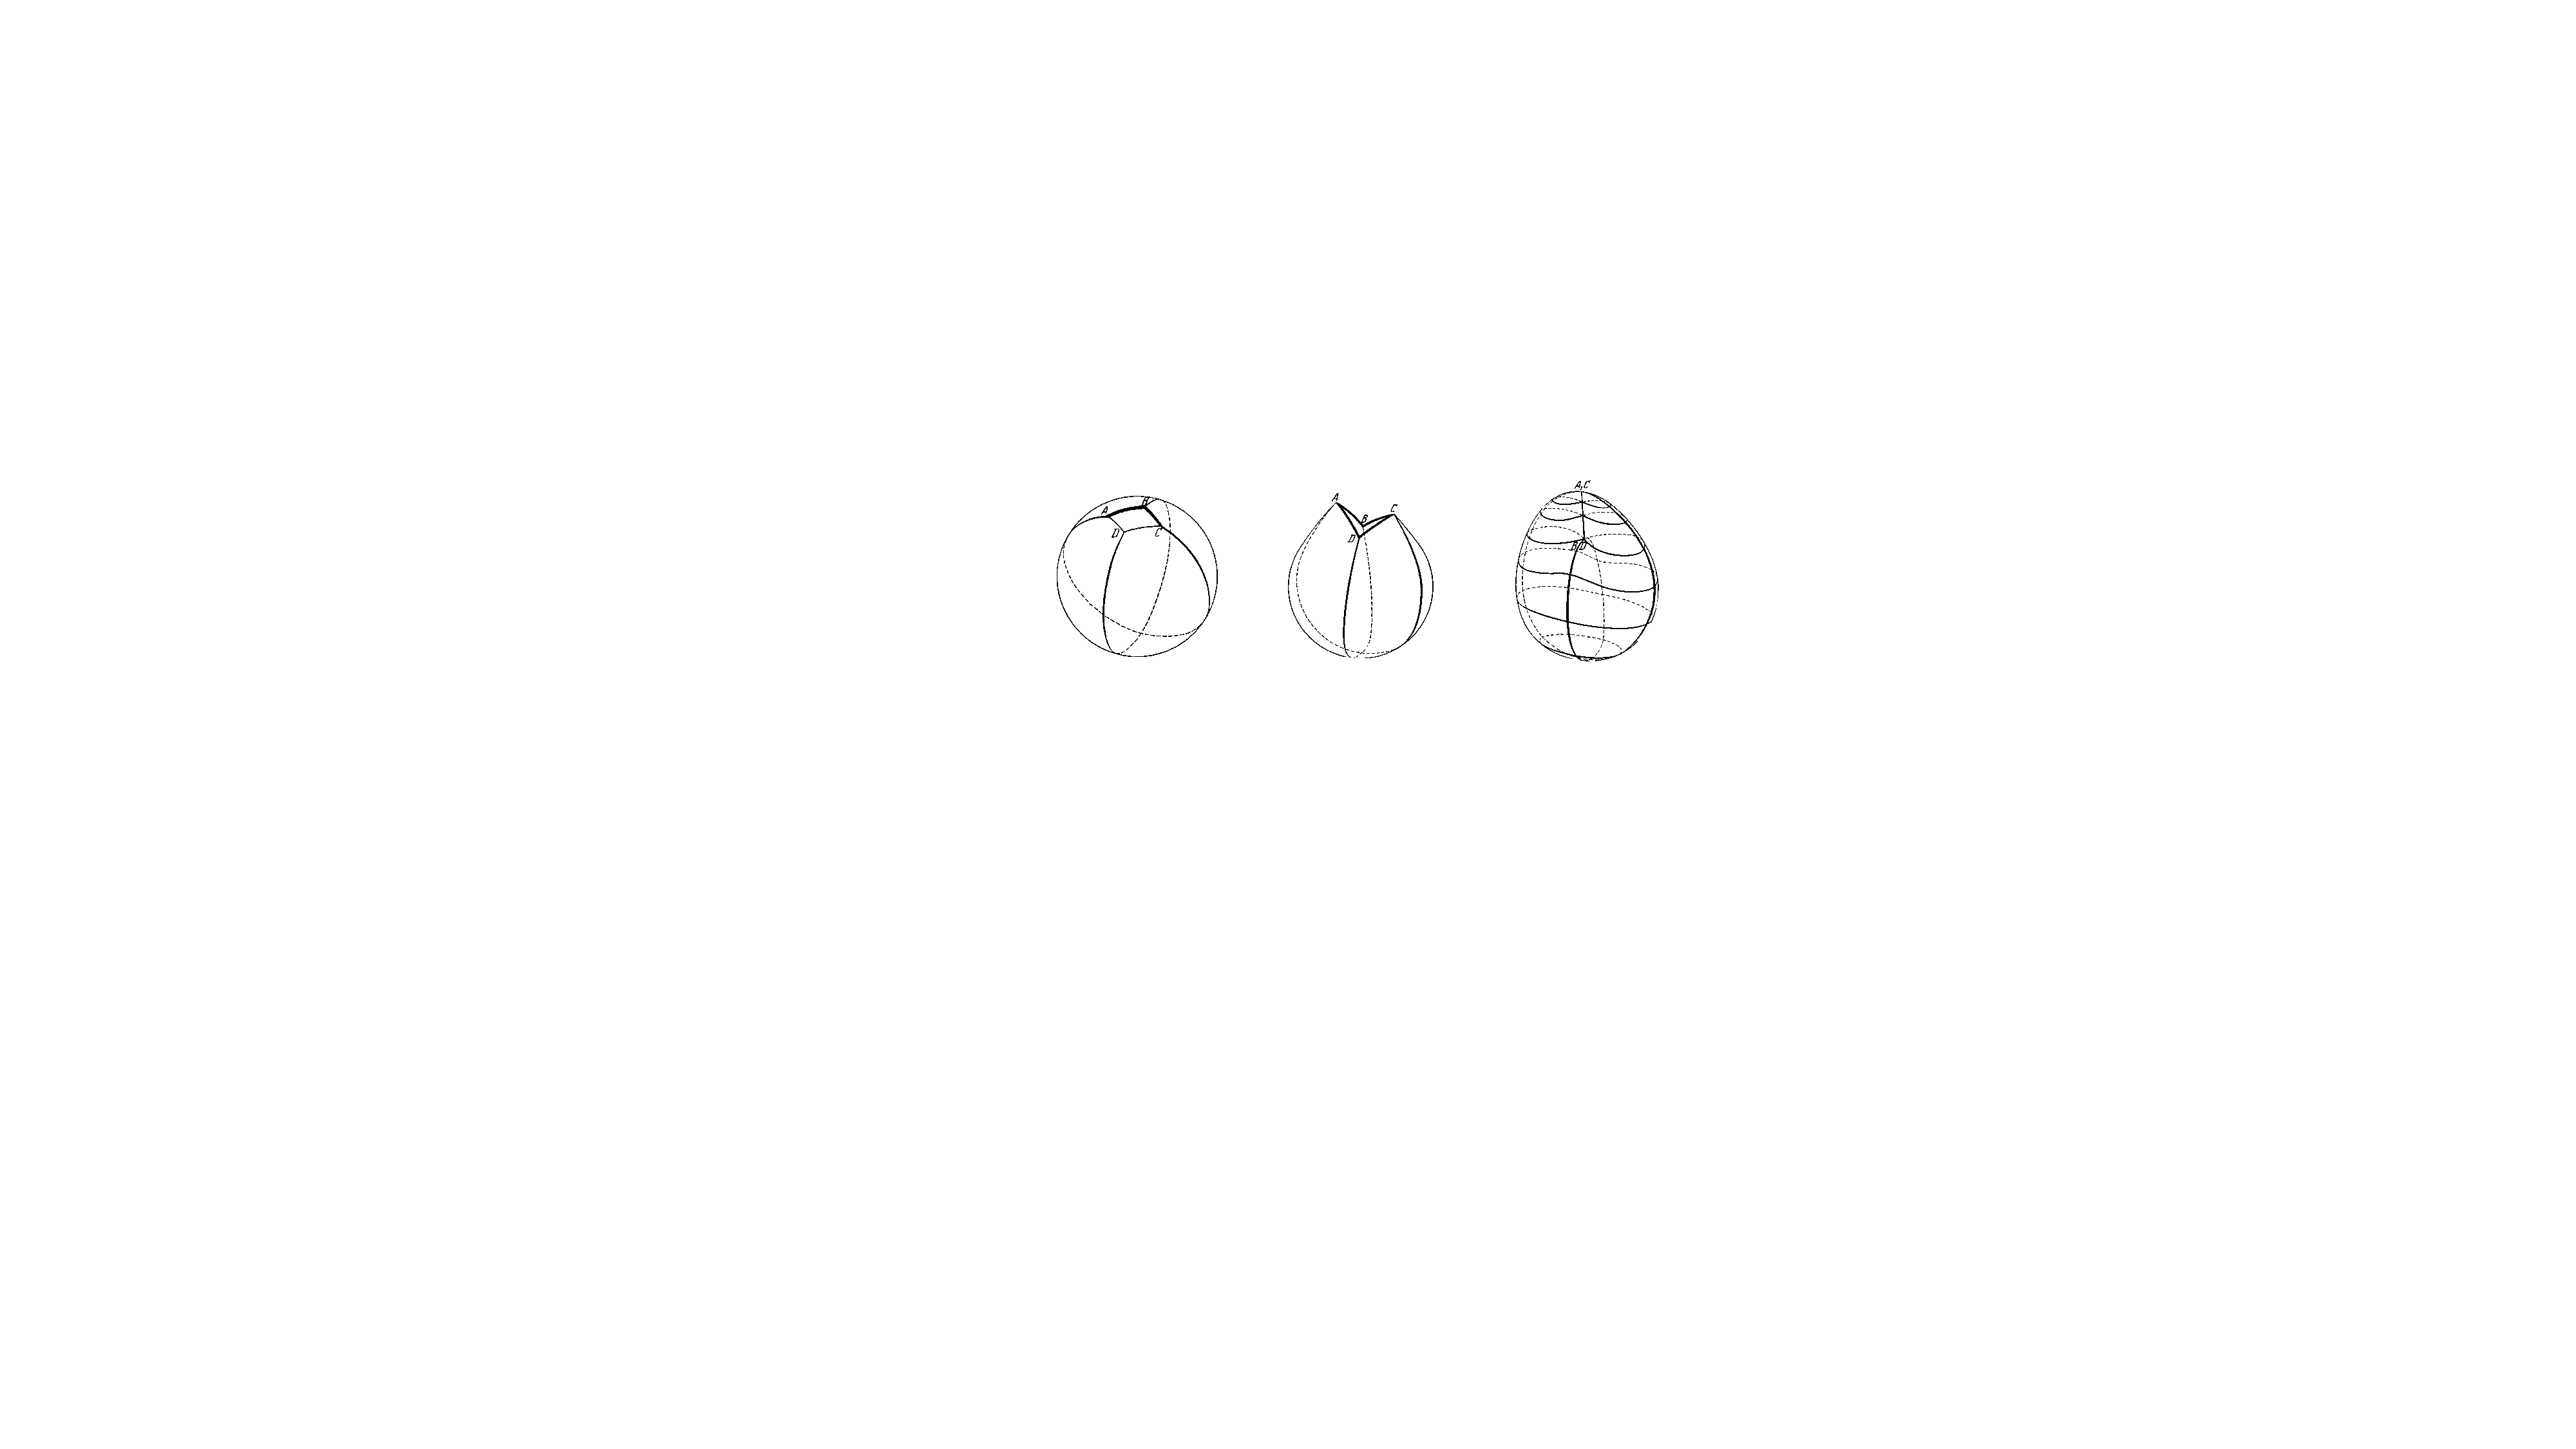
\includegraphics[scale=0.6]{Images/crosscap.pdf}
    \caption{Construction of the projective plane out of a disk. Adding a hole to this surface creates a crosscap, which is homeomorphic to a M\"bius band, see Exercises~\ref{RP2 exercise} and \ref{crosscap exercise}.}
    \label{fig:crosscap}
\end{figure}
\begin{example}{{{\cite[Exercise III.3]{Bredon}}}}
    Consider an annulus. Identify antipodal points on the outer circle. Also identify antipodal points on the inner circle. Calculate the fundamental group of this surface. Is it homeomorphic to any of the orientable compact surfaces? \emph{Hint:} taking $U$ and $V$ to be overlapping annular neighborhoods of the two boundaries of the annulus, the generator of $\pi_1(U\cap V)$ is mapped to the square of the generator in $\pi_1(U)$ and similarly in $\pi_1(V)$; therefore $\pi_1(U\cup V)=\langle a,b\mid a^2=b^2\rangle$.
\end{example}
\begin{xca}[{{\cite[Exercise 1.20]{Hatcher}}}]
    Let $X$ be the subspace of $\bbR^2$ that is the union of the circles $C_n$ of radius $n$ and center $(n, 0)$ for $n = 1, 2, \ldots$. Show that $\pi_1( X )$ is the free group $\ast_n \pi_1( C_n )$, the same as for the infinite wedge sum $\bigvee_{i=1}^\infty \bbS^1$. Show that $X$ and $\bigvee_{i=1}^\infty \bbS^1$ are in fact homotopy equivalent, but not homeomorphic.
\end{xca}

\begin{example}[Hawaiian earring {{\cite[Example 1.25]{Hatcher}}}]\label{hawaiian earring}
    Let $X$ be the subspace of $\bbR^2$ that is the union of the circles $C_n$ of radius $1/n$ and center $(1/n, 0)$ for $n = 1, 2, \ldots$. Initially this space can be mistaken for the infinite wedge sum $\bigvee_{i=1}^\infty \bbS^1$, but in fact it has a much larger fundamental group. This is because in the topology induced from $\bbR^2$ it is possible for a continuous loop $\gamma[0,1]\to X$ to cover an infinite number of circles $C_n$ at once, unlike in the case of the wedge sum. As a result, $\pi_1(X)$ can be mapped surjectively onto the infinite direct product group $\prod_{n=1}^\infty \bbZ$, which is uncountably large. 
\end{example}

\begin{example}[Torus knots {{\cite[Example 1.24]{Hatcher}}}]
    For relatively prime integers $m,n$, the \emph{torus knot}\index{Torus knots}\index{Knot!torus} $K=K_{m,n}\subset \bbR^3$ is the image of the embedding $f:\bbS^1\to \bbS^1\times \bbS^1\cong \bbT^2\subset\bbR^3$ given by $f(z)=(z^m,z^n)$ ($z=\rme^{2\rmi\pi t}$), where the torus $T$ is embedded in space in the standard way. Let us compute $\pi_1(\bbR^3\setminus K)$. First, we can safely replace $\bbR^3$ with its compactification $\bbS^3$ by adding ``a point at infinity''. This isomorphism follows from the Seifert-van~Kampen theorem. Now we may decompose $\bbS^3\setminus \bbT^2$ into two open solid tori $U,V$. Let $C$ be an open tubular neighborhood of $T\setminus K$. Then $U\cup C$ and $V\cup C$ form an open covering of $\bbS^3\setminus K$ with a path connected intersection. The fundamental groups of $U\cup C$, $V\cup C$, and the intersection $C$ are all isomorphic to $\bbZ$ and generated by loops $x,y,z$, respectively. The inclusions of $C$ into $V\cup C$ or $U\cup C$ map $z$ to $x^m$ or $y^n$. Therefore $\pi_1(\bbS^3\setminus K)=\langle x,y\mid x^m=y^n\rangle$. The center of this group is the subgroup generated by the element $x^m=y^n$, and the factor by the center is exactly $\bbZ_m\ast\bbZ_n$. By commuting all powers of $x^m$ through to the left, the elements of this group can be uniquely represented by strings of the form $x^{mk}y^{l_0}x^{k_1}y^{l_1}x^{k_2}y^{l_2}\cdots$ where $k\in\bbZ$, $k_i\in {0,\ldots,m}$ and $l_i\in\{0,\ldots,n\}$.
\end{example}

\begin{example}[Lens spaces {{\cite[Exercise III.10]{Bredon}}}]\label{example Lens space bredon}
    Let $X=(\bbD^2\times \bbS^1)\sqcup_f (\bbD^2\times \bbS^1)$ be the gluing of two solid tori along the map $f:\bbS^1\times \bbS^1\to \bbS^1\times \bbS^1$ induced from the linear map $\bbR^2\to\bbR^2$ given by an integer matrix $\begin{pmatrix}a&b\\c&d\end{pmatrix}$. The fundamental group of a solid torus are generated by one generator, call it $\gamma_1$ and $\gamma_2$ for the two solid tori correspondingly; in addition, the two solid tori overlap by a space that deformation retracts onto a torus $\bbT^2$ whose fundamental group is generated by two simple generators $\alpha$ and $\beta$; assuming $a\neq 0$, by Seifert-van~Kampen, from one inclusion we have the mappings $\alpha\mapsto\gamma_1$ and $\beta\mapsto e$, whereas from the other we get $\alpha\mapsto \gamma_2^d$ and $\beta\mapsto \gamma_2^c$. The resulting identification $\gamma_1\sim \gamma_2^d$ simply allows us to drop $\gamma_1$ from the list of generators. Thus $\pi_1(X)$ is the cyclic group $\langle \gamma_2\mid \gamma_2^c\rangle=\bbZ_c$. Note that the case $a=0$ is special -- in that case $\pi_1(X)=\bbZ$. If the matrix of $f$ is invertible (which is true iff $\det f=\pm1$) and is parametrized as $\begin{pmatrix}q&(qq'-1)/p\\p&q'\end{pmatrix}$, the resulting space is the so called \emph{lens space}\index{Lens spaces} $L(p;q)$ with fundamental group $\bbZ_p$. We have $L(1;0)=\bbS^3$ ($f=\id$) and $L(2;1)=\bbR P^3$ ($f=-\id$).
\end{example}





\newpage

\section{Manifolds}

\subsection{Topological manifolds}
\begin{defn}[Locally Euclidean Space]\index{Locally Euclidean Space}
A topological space $X$ is locally $n$-dimensional Euclidean if every $x\in X$ has an open neighborhood homeomorphic to the open $n$-dimensional ball, $U_x\cong B^n$. 
\end{defn}
\begin{defn}[Second-countability]\index{Second countable space}
A topological space is called second countable if it has a countable basis of topology.
\end{defn}
\begin{defn}[Paracompactness]\index{Paracompact space}
\begin{enumerate}
    \item A collection of subsets $A_\alpha, \alpha \in I,$ of $X$ is called locally finite if every $x\in X$ has an open neighborhood $U_x$ such that $U_x\cap A_\alpha \neq \varnothing$ only for a finite number of $\alpha$'s. If all $A_\alpha$'s are open, this is the same as $x$ being an element of only finitely many of them.
    \item Given an open covering $\{U_\alpha\}$ (i.e.\ a collection of open sets such that $\bigcup_\alpha U_\alpha=X$), a refinement of it is an open covering $\{V_\beta \}$ such that $\forall \beta \;\exists \alpha: V_\beta \subset U_\alpha $.
    \item $X$ is called paracompact if every open covering of $X$ admits an open, locally finite refinement.
\end{enumerate}
\end{defn}
\begin{defn}[Topological manifold]\index{Manifold!topological}
A topological manifold is a second countable, Hausdorff, locally Euclidean space.
\end{defn}
The following proposition is the reason why second countability is often substituted with paracompactness in the definition of manifolds.
\begin{prop}
All topological manifolds are paracompact (and locally compact).
\end{prop}
\begin{proof}
See \cite[Thm. 1.15]{Lee}
\end{proof}
\begin{defn}[Charts]\index{Chart}
Let $X$ be an $n$-dimensional topological manifold. A \emph{chart} on it is a pair $(U,\varphi)$, where $U\subset X$ is an open set and $\varphi:U\to \bbR^n$ is a continuous map (called the chart map) that is also a homeomorphism onto its image $\wh{U}=\varphi (U)$, i.e.\ $U\cong \varphi(U)=\wh{U}$. The chart is called a \emph{coordinate ball} if $\wh U$ is a ball in $\bbR^n$. The values of $\varphi$ are called \emph{coordinates} of the corresponding points on $X$.
\end{defn}
\begin{rem}
Since $X$ is locally Euclidean, every point $x$ automatically has a chart $(U_x,\varphi)$ around it. In particular, every manifold has an open covering by charts $(U_\alpha,\varphi_\alpha)$.
\end{rem}

\begin{thm} All topological manifolds have the following properties.
\begin{enumerate}
    \item There is a countable basis consisting of coordinate balls (it can also be made locally finite and every ball can be made precompact)
    \item Local compactness.
    \item Local path-connectedness (i.e.\ every point has a path-connected neighborhood).
    \item At most countably many connected components, each open and a topological manifold of its own.
    \item The fundamental group $\pi_1(X)$ is at most countable.
\end{enumerate}
\end{thm}
\begin{proof}
1,2) Pick an open covering by charts $\{U_\alpha\}$. Each $U_\alpha $ can be covered by countably many coordinate balls $V_{\alpha_i}$ because $\wh{U}_\alpha$ can be covered by countably many balls in $\bbR^n$. By second countability, there is a countable subcovering and basis $\{V_\beta\}$. Fixing a chart $U$ and covering it by coordinate balls $V_\alpha$, we have that $\xoverline{V}_\beta$ is compact in $U$ (because it's homeo to a closed ball), therefore closed in $X$ by Hausdorffness. Therefore it's also compact in $X$, i.e.\ $V_\beta$'s are precompact. The covering can also be made locally finite: let $\{K_i\}_{i=1}^\infty$ be an exhaustion of $M$ by compact sets (i.e.\ $\bigcup_i K_i=M$; we will prove the existence in Prop. \ref{prop.exhaustion}). After picking out a finite subcovering of every compact ``stripe'' $K_{i+1}\setminus \Int K_{i}$ by charts that are small enough to fit within the wider open ``stripe'' $\Int K_{i+2}\setminus K_{i-1}$ (possible because all charts still form a basis), we end up with a locally finite covering (since every point of the manifold is contained only in 3 of the open stripes).

3) Obvious because balls are.

4) 2nd countability implies countable components. The rest is obvious.

5) See \cite[Thm 1.16]{Lee}.
\end{proof}

\begin{lem}
Locally path-connected and connected $\Leftrightarrow$ path-connected.
\end{lem}
\begin{proof}
The reverse direction is obvious. In the forward direction, introduce the set $C=\{q:q\text{ is connected with }p\}$  for some fixed $p\in X$. We will prove that $C$ is clopen and therefore equal to $X$.

$C$ is open because $X$ is locally path-connected.
$C$ is closed because for any $z\in\xoverline{C}$ there is a path-connected neighborhood $U_z$, thus $U_z\cap C\neq \varnothing$, and $z\in C$. Therefore $\xoverline C=C$. 
But $X$ is connected, and $C$ is clearly not empty, therefore $C=X$, and lastly $C$ is path-connected by definition.
\end{proof}
\begin{cor}
For manifolds, connectedness is equivalent to path-connectedness. In particular, connected components of manifolds are path-connected.
\end{cor}

\begin{example}
\begin{enumerate}
    \item Any open set in $\bbR^n$ is a manifold.
    \item $\bbS^n$ is a manifold because it can be covered by finitely many charts $(U_i,\varphi_i)$, where $U_i$ is an open hemisphere whose ``equator'' lies on one of the coordinate hyperplanes, and $\varphi_i$ is simply the orthogonal projection to that hyperplane.
    \item An $n$-dimensional torus $\bbT^n=(\bbS^1)^{\times n}$ is a manifold.
    \item The figure eight, 8, as a subset of $\bbR^2$, is not a manifold, because its center doesn't have a neighborhood homeomorphic to an interval.
    \item Matrices $\Mat(n,\bbR )$ form an $n^2$-dimensional manifold (isomorphic to $\bbR^{n^2}$). So do invertible matrices $\GL(n,\bbR )$ (being an open subset in $\bbR^{n^2}$) and all other classical matrix groups.
\end{enumerate}
\end{example}

\subsection{Smooth structures}
\begin{defn}[Atlas]\index{Atlas!topological}
An atlas $\mathcal{A}$ for a topological manifold $M$ is a collection of continuous charts $\{(U_\alpha,\varphi_\alpha)\}$, $\varphi_\alpha:U_\alpha\to \wh{U}_\alpha \subset \bbR^n$ such that $\bigcup_\alpha U_\alpha =M$.
\end{defn}
Throughout these notes we also adopt the notation where for any atlas as above, $U_{\alpha\beta}=U_\alpha \cap U_\beta$, $U_{\alpha\beta\gamma}=U_\alpha \cap U_\beta \cap U_\gamma$, etc.

\begin{defn}[Smooth atlas]\index{Atlas!smooth}
An atlas is called smooth (or of class $C^k$ or $C^\omega$) if all of the \emph{transition functions} $\varphi_{\beta\alpha}=\varphi_\beta\circ\varphi_\alpha^{-1}:\varphi_\alpha(U_{\alpha\beta})\to\varphi_\beta(U_{\alpha\beta})$ are smooth/$C^\infty$ (of class $C^k$, or real analytic, respectively) in the sense of multivariable calculus on $\bbR^n$.
\end{defn}
\begin{defn}[Equivalent atlases]\index{Atlas!equivalence of}
Two atlases $\mathcal{A}_1$ and $\mathcal{A}_2$ are called equivalent, or compatible, if $\mathcal{A}_1\cup\mathcal{A}_2$ is still an atlas of the same smoothness class.
\end{defn}
\begin{defn}[Differentiable structure]\index{Differentiable structure}\index{Smooth structure}
A smooth ($C^k$, analytic) structure on a topological manifold $M$ is an equivalence class $[\mathcal{A}]$ of smooth (respectively, $C^k$, $C^\omega$) atlases on it. 
\end{defn}
\begin{defn}[Smooth manifold]\index{Manifold!smooth}
A smooth manifold is a pair $(M,[\mathcal{A}])$ consisting of a topological manifold and a smooth structure.
\end{defn}

\begin{rem}
    Recall that the second countability of topological manifolds implies their paracompactness (but not vice versa). In the case of differentiable manifolds, these properties turn out to be equivalent, and also equivalent to metrizability, or to the existence of smooth partitions of unity (see next section). This is why the definitions sometimes differ.
\end{rem}

\begin{example}
\begin{enumerate}
    \item Let $\psi:\bbR \to\bbR $ be $\psi(x)=x^3$. Then $\{(\bbR ,\psi)\}$ is an atlas that defines a smooth structure on $\bbR $. It is not smoothly compatible with the standard smooth structure given by the chart map $\varphi(x)=x$, because the transition function $\varphi\circ \psi^{-1}(x)=x^{1/3}$ is not smooth. Therefore $\bbR $ has many (in fact, infinitely many) different smooth structures.
    \item Any real or complex vector space is automatically a smooth manifold.
    \item Spaces of matrices, classical groups, spheres... are all smooth manifolds with their standard structures.
    \item Not every topological manifold admits a smooth structure, although examples are pretty difficult to construct. On the other hand, any $C^1$ manifold admits a compatible (in the $C^1$ sense) smooth structure, which is unique up to diffeomorphism (see below). This is why even mathematicians are mostly happy working with just either topological or immediately smooth/analytic manifolds. Interestingly, all topological manifolds in dimensions 1,2, and 3 admit unique (up to diffeo) smooth structures.
    \item All Lie groups (defined as smooth manifolds with a group structure in which multiplication and inversion are smooth maps) in fact support a unique (up to diffeo) $C^\omega$ structure. This is an immediate consequence of the convergence of the Baker-Campbell-Hausdorff series.
\end{enumerate}
\end{example}

From now on we work only with smooth manifolds, and use the word ``manifold''  to mean ``smooth manifold''.
\begin{defn}[Smooth maps]\index{Smooth map}
Let $M$ and $N$ be two manifolds with atlases $\{(U_\alpha,\varphi_\alpha)\}$ and $\{(V_\beta,\psi_\beta)\}$, respectively. A map $f:M\to N$ is called smooth if all of its \emph{local representatives} $f_{\beta\alpha}=\psi_\alpha\circ f\circ \varphi_\beta^{-1}:\wh{U}_\beta\to \wh{U}_\alpha$ are smooth. The set of all smooth maps between two manifolds is denoted by $C^\infty (M,N)$. When $N=\bbR $, we write $C^\infty(M)=C^\infty (M,\bbR )$ for the space of ``smooth functions''. The category $\mathsf{Man}^\infty$ is the category of smooth manifolds with smooth maps for morphisms.
\end{defn}
\begin{xca}
Check that all chart maps in any atlas of a smooth manifold $M$ are smooth as maps from $M$ to the standard $\bbR^n$.
\end{xca}
\begin{rem}
The above exercise illustrates the general alternative approach to manifolds: instead of defining a smooth structure in terms of charts, we could describe it by specifying \emph{what smooth functions should be} by describing the subsets of the sets of local continuous functions $C(U_\alpha)$ that we want to be smooth (more precisely, one has to pick a subsheaf of the sheaf of continuous functions that is locally isomorphic to the sheaf of smooth functions on $\bbR^n$).
\end{rem}
\begin{defn}[Manifolds with boundaries]\index{Manifold!with boundaries/corners}
Let $\bbR_+^n$ be the closed upper half-space in $\bbR^n$ (i.e.\ $x^n\geq 0$). An $n$-dimensional manifold with boundaries is defined just like a smooth manifold, only now some of the chart maps can map to $\bbR_+^n$. The smoothness of boundary transitions is characterized as follows: any function $\bbR_+^n\to \bbR_+^n$ is called smooth if it can be extended as a smooth function into an open neighborhood of $\bbR_+^n$. The set of points of $M$ that map to the boundary of $\bbR_+^n\subset \bbR^n$, i.e.\ the hyperplane $x^n=0$, is called the boundary $\partial M$. We also denote the interior by $\mathring M=M\setminus \partial M$.
\end{defn}
\begin{example}
$\sqrt{y}:\bbR_+\to\bbR $ is not smooth on $\bbR_+$ with the standard smooth structure. However, it can be taken to be the chart map defining a new smooth structure on $\bbR_+$, and in that new structure it'll become smooth, because its local representative will be the identity map.
\end{example}
\begin{rem}
Similarly, one can define \emph{manifolds with corners} using chart maps that can take values in quadrants, octants, and so on, of $\bbR^n$.
\end{rem}

\begin{defn}[Diffeomorphisms]\index{Diffeomorphism}
A smooth map $f:M\to N$ between manifolds is a called a diffeomorphism if it has a smooth inverse. They are the isomorphisms in $\mathsf{Man}^\infty$.
\end{defn}
\begin{prop}
\begin{enumerate}
    \item Diffeos are homeo and open.
    \item If $M$ and $N$ have boundaries and $f:M\to N$ is a diffeo, then $f(\partial M)=\partial N$ and $\restr{f}{\mathring M}: \mathring M\to \mathring N$ is a diffeo.
\end{enumerate}
\end{prop}
\begin{example}
\begin{enumerate}
    \item Different smooth structures can be diffeomorphic! Take $\bbR $ with the chart $\psi(x)=x^3$ that we considered earlier. It is diffeomorphic to the standard smooth structure given by the chart $\varphi(x)=x$, and the diffeomorphism is given by $\psi$ itself! Indeed, its local representative in the two charts is $\varphi\circ \psi \circ\psi^{-1}(x)=x$. In this manner one can show that there is only one smooth structure on $\bbR$ up to diffeomorphism.
    \item Historically the first manifolds to be found to support more than one non-diffeomorphic smooth structure were spheres, starting with $\bbS^7$ which has 28 diffeomorphism classes of smooth structures. These smooth structures are now known as Milnor's \emph{exotic spheres}.
    \item $\bbR^n$ has only one smooth structure up to isomorphism for all $n\neq 4$. For $n=4$, it admits \emph{uncountably many} non-diffeomorphic structures. This makes the study of four-dimensional topological manifolds especially sophisticated, and there are still many very fundamental unsolved problems in four-dimensional topology \cite{smooth.structures}.
    \item In every dimension $n\geq 4$ there exist \emph{compact} topological manifolds that don't admit any compatible smooth structure.
\end{enumerate}
\end{example}

\begin{xca}
    Show that $\bbS^1$ supports only one smooth structure up to diffeomorphism.
\end{xca}


\subsection{Partitions of unity}

First we note that on $\bbR^n$ there exist bump functions, i.e.\ for any point $x_0$ and any two radii $0<r_1<r_2$ there is a function $\eta\in C^\infty(\bbR^n)$ such that $\restr{\eta}{B_{r_1}(x_0)}=1$ and $\restr{\eta}{\bbR^n\setminus \overline{B_{r_2}}(x_0)}=0$.
\begin{xca}
    Using the function $\int_a^x \rme^{\frac{1}{(x'-a)(b-x')}} \dd x'$ defined on $(a,b)$, construct a general bump function for $\bbR^n$.
\end{xca}

Now, any manifold $M$ can be covered by a locally finite collection of coordinate balls $(U_\alpha,\varphi_\alpha)$. Let $\eta_\alpha$ be a bump function that equals $0$ outside of the ball $\wh{U}_\alpha\subset \bbR^n$. Then define the smooth functions
\[f_\alpha =\begin{cases} \eta_\alpha\circ\varphi_\alpha, & \text{on }U_\alpha, \\ 0, & \text{on }M\setminus U_\alpha.\end{cases}\]
Finally, we normalize this collection of functions by defining
\[\chi_\alpha(x)=\frac{f_\alpha(x)}{\sum_\alpha f_\alpha (x).}\]
This expression is well-defined because the sum in the denominator is finite for every fixed $x$. These functions have the following properties:
\begin{enumerate}
    \item $\chi_\alpha\in C^\infty(M)$,
    \item $0\leq \chi_\alpha\leq 1$,
    \item $\supp \chi_\alpha\subset U_\alpha$,
    \item $\{\chi_\alpha\}$ is locally finite, i.e.\ only finitely many of them are non-zero at any given point $x\in M$,
    \item $\sum_\alpha \chi_\alpha (x)\equiv 1$.
\end{enumerate}

\begin{defn}[Partition of unity]\index{Partition of unity}
    Any collection of functions satisfying the above list of properties is called a \gls{pou} subordinate to the open covering (not necessarily by coordinate balls) $\{U_\alpha\}$ of $M$.
\end{defn}

\begin{prop}[{{\cite[Thm.~4.85]{LeeTop}}}]
    Any open covering of a paracompact Hausdorff space admits a subordinate \gls{pou}.
\end{prop}

\begin{prop}
    Any open covering of a smooth manifold admits a subordinate partition of unity.
\end{prop}
\begin{proof}
    Any open covering has a locally finite refinement consisting of coordinate balls, which allows us to apply the construction above to the refinement. Notice that second countability is key to the existence of partitions of unity.
\end{proof}
\begin{thm}[Extension lemma]\label{extension lemma}\index{Extension lemma}
    Let $A\subset M $ be a closed subset, and $f\in C^\infty(A,\bbR^k)$. Then for any open $U$ such that $A\subset U$, there exists an extension $\wt{f}\in C^\infty(M,\bbR^k)$: $\restr{\wt{f}}{A}=f$, such that $\supp \wt{f}\subset U$.
\end{thm}
\begin{proof}
    Pick $p\in A$ and neighborhood $U_p\subset U$. Let $\wt{f}_p: U_p\to\bbR^k$ be a smooth extension of $f$ from $U_p\cap A$. It is guaranteed to exist for sufficiently small $U_p$ by definition of smoothness on closed subsets of $\bbR^n$ and smoothness of chart maps.

    Then $\{U_p\}_{p\in A}\cup \{M\setminus A\}$ is an open covering of $M$. Let $\{\chi_p\}\cup\{\chi_0\}$ be a \gls{pou} subordinate to this covering (and $\chi_p=0$ inevitably for almost all $p$ so that the resulting collection is locally finite). Therefore $\chi_p\cdot \wt{f}_p:U_p\to\bbR^k$ are smooth and vanishing at the boundary of $U_p$, which allows us to extend them by zeros to smooth functions on all $M$. Finally, $\wt{f}=\sum_{p\in A} \chi_p \wt{f}_p$ is the extension we seek with support inside $U$.
\end{proof}
\begin{defn}[Exhaustion function]\index{Exhaustion}
    A function $f\in C^\infty(M)$ is called an exhaustion function for $M$ if for every $c\in\bbR $ the pre-image $f^{-1}((-\infty,c])$ is relatively compact (i.e.\ has compact closure in $M$).
\end{defn}
\begin{prop}\label{prop.exhaustion}
    Every smooth manifold has an exhaustion function.
\end{prop}
\begin{proof}
    Let $\{V_\alpha\}$ be a countable open covering by precompact sets and $\{\chi_\i\}_{i=1}^\infty$ a subordinate \gls{pou}. Define $f(x)=\sum_{n=1}^\infty n\cdot \chi_n(x)$. 

    Clearly $f^{-1}((-\infty,c])\subset \bigcup_{i=1}^{[c]+1}\xoverline{V_i}$, which is a compact set.
\end{proof}

\subsection{Sard's theorem}

In $\bbR^n$, a set $A$ is said to have\emph{ zero measure} if for any $\epsilon>0$ it can be covered by a collection of open balls $B_i$ such that the total volume of these balls is less than $\epsilon$.

\begin{defn}[Measure zero]
    Even though there is no canonical way to measure volumes on manifolds, there is still a consistent notion of zero measure. Namely, a set $A\subset M$ has zero measure if all the sets $\varphi_\alpha(A\cap U_\alpha)$ are measure zero in $\bbR^n$ for an atlas $\{(U_\alpha,\varphi_\alpha)\}$.
\end{defn}

\begin{defn}[Rank of a map]\label{def.rank}\index{Rank of a map}
    Let $f\in C^\infty (M^m,N^n)$ (superscripts here indicate the dimensions of the manifolds). We say that the rank of $f$ at $p\in M$ is $\rank_p f=r$ if there exist two local charts, $(U,\varphi)$ around $p \in M$ and $(V,\psi)$ around $f(p)\in N$, such that the local representative of $f$ in these charts is $\psi\circ f\circ\varphi^{-1}(x^1,\ldots,x^m)=(x^1,\ldots,x^r,\underbrace{0,\ldots,0}_{n-r})$.
\end{defn}

\begin{defn}[Critical and regular points/values]\index{Critical points/values}\index{Regular points/values}
    $p\in M$ is said to be a critical point of $f\in C^\infty(M^m,N^n)$ if $\rank_p f<n$, i.e.~if its differential at $p$ is not surjective. In this case, $f(p)\in N$ is called a critical value of $f$. Otherwise, $p$ is a regular point, and a regular value is one all of whose pre-images are regular points.
\end{defn}

The main property of regular values of smooth maps is that they are generic, as demonstrated by the following deep theorem. We will need this result when we talk about transversality in the context of fiber bundles.

\begin{thm}[Sard]\index{Theorem!Sard}\label{thm sard}
    For any $f\in C^\infty(N,M)$ the set of critical values (also known in some contexts as the \emph{caustic}) of $f$ has measure zero in $M$.
\end{thm}
\begin{proof}
    This theorem is essentially entirely local, i.e.\ it suffices to prove it for $N=\bbR^n$ and $M=\bbR^m$. Every manifold can be broken up into a countable number of neighborhoods, and a countable union of sets of measure zero is still measure zero.

    Let $C\subset \bbR^m$ be the set of critical points of $f:\bbR^n\to \bbR^m$ and pick $x_0\in C$. Then, after some rotation of the space, we can assume that its derivative maps $f'_{x_0}(\bbR^n)=\bbR^k\times \{0\}\subset \bbR^m$, where $k\leq n-1$ is the rank of the Jacobi matrix at $x_0$.  If we choose a ball $B_r(x_0)$ of radius $r$ around $x_0$, then
    \[f'_{x_0}(B_r(x_0))\subset (\bbR^k\times \{0\})\cap B_\epsilon(f(x_0)),\quad \epsilon=r\cdot \mathrm{Lip}f,\]
    where $\mathrm{Lip}f$ is the Lipschitz constant of $f$ inside $B_r(x_0)$ (equal to the supremum of all directional derivatives in unit directions). We only need the existence of such an $\epsilon$ and that it goes to zero with $r\to 0$.

    Therefore $f'_{x_0}(B_r(x_0))$ can be covered by $N^k$ cubes of diameter $\epsilon/N$. By differentiability there exists $\delta>0$ such that 
    \[\lvert f(y)-f(x_0)-f'_{x_0}(y-x_0)\rvert\leq \frac{1}{N}|y-x_0|,\quad \text{ for all }y\in B_\delta(x_0).\]
    So $f(y)$ is within $r/N$ distance of the hyperplane $f(x_0)+f'_{x_0}(\bbR^n)$ (provided that $r<\delta$). Therefore the image $f(B_r(x_0))$ itself is contained in a neighborhood of $f'_{x_0}(B_r(x_0))$ of radius $r/N$. Thus we can construct $N^k$ disjoint sets $E_j$ of diameter $\sim r/N$ that cover $f(B_r(x_0))$.

    We repeat the above for every point $x\in C$ and get $r_x>0$ such that $f(B_{r_x}(x))\subset \bigsqcup_{j=1}^{N^k}E_j^x$. By \href{https://en.wikipedia.org/wiki/Vitali_covering_lemma}{Vitali's covering lemma}, there is a countable subcovering, so $C\subset \bigsqcup_{i=1}^\infty B_{r_i}(x_i)$ such that $\{B_{r_i/5}(x_i)\}$ are disjoint and for every $i$ there are sets $E^i_j,j=1,\ldots,N^k$ such that $\mathrm{diam}(E^i_j)\sim r/N$ and $f(B_{r_i}(x_i))\subset \bigsqcup_{j=1}^{N^k}E^i_j$. Thus $f(C)\subset \bigsqcup_{i=1}^\infty\bigcup_{j=1}^{N^k}E_j^i$. We can safely assume that $C\subset [-l,l]^n$ for some $l\in \bbN$ (otherwise it can be broken up into countably many pieces of this kind, which won't upset the result of the theorem). By compactness we can then assume that $r_x<1$ for all $x\in C$. Thus
    \begin{multline}
        \mathrm{volume}(f(C))\leq \sum_{i,j}(\mathrm{diam}(E^i_j))^n\leq \sum_{i,j}\left(\frac rN\right)^n\lesssim \sum_{i}N^k\frac{r^n}{N^n}\lesssim \\
        \lesssim 5^nN^{k-n}\sum_i\frac{r^n}{5^n}\lesssim 2\cdot 5^n N^{k-n}\cdot \mathrm{volume}([-l,l]^n),
    \end{multline}
    since $C$ lies inside $[-l,l]^n$ and is covered by balls of radii $r_i\leq 1$ with disjoint sub-balls, so the sum of the volumes of these sub-balls can only exceed the volume of $[-l,l]^n$ by at most a constant factor (coming from pieces that stick out of $[-l,l]^n$), say $2$.

    But now, $k<n$, thus in the limit $N\to \infty$ we find that the volume of $f(C)$ has to be zero. This proof is due to Behnam Esmayli, a more conventional one can be found in \cite[Thm.~6.10]{Lee}.
\end{proof}
\begin{rem}
    The ability to globalize the proof of this theorem depends crucially on second countability. Indeed, we could consider a non-second-countable 1-dimensional ``manifold'' given by the uncountable disjoint union of lines $M=\bigsqcup_{a\in \bbR} R_a=\bigsqcup_{a\in \bbR} \bbR$, and define a function $f:M\to \bbR$ by $\restr{f}{R_a}=a$. In this case $f$ is smooth and every value $a\in\bbR$ is a critical value, contrary to Sard's theorem. What happened was that we found an uncountable family of local neighborhoods ($R_a$), for each of which the set of critical values has measure zero (one point $a$). But the union of an uncountable number of sets of measure zero can have nonzero measure. Thus second countability is key to Sard's theorem working on general manifolds.
\end{rem}






\subsection{Inverse \& Implicit Mapping Theorems}

In this section we just recall the statements of two basic theorems in multivariable calculus.
\begin{thm}[\Gls{inmt}]\label{InMT}\index{Theorem!Inverse mapping}
    Let $U,V\subset\bbR^n$ be open and $f\in C^\infty(U,V)$. If the Jacobi matrix $\frac{\partial f^i}{\partial x^j} (a)$ is invertible for some $a\in U$, then there are neighborhoods $a\in U_a\subset U$ and $f(a)\in V_{f(a)}\subset V$ such that $\restr{f}{U_a}:U_a\to V_{f(a)}$ is a diffeomorphism.
\end{thm}
Meaning: any smooth map whose Jacobi matrix is non-singular at a point is locally a diffeomorphism around that point.

\begin{thm}[\Gls{immt}]\label{ImMT}\index{Theorem!Implicit mapping}
    Let $U\subset \bbR^n\times \bbR^k$ be open, $(x,y)=(x^1,\ldots,x^n,y^1,\ldots,y^k)\in U$. Let $\Phi\in C^\infty(U,\bbR^k)$ and $\Phi(x,y)=c$. If the matrix $\left(\frac{\partial\Phi^i}{\partial y^j}(x,y)\right)_{i,j=1}^k$  is non-singular, then there are open neighborhoods $x\in V_x\subset \bbR^n$ and $y\in W_y\subset\bbR^k$ and a smooth map $f\in C^\infty (V_x,W_y)$ such that 
\[\forall\,(v,w)\in V_x\times W_y,\;\; \Phi (v,w)=c \Leftrightarrow w=f(v).\]
\end{thm}
Meaning: the equation $\Phi(x,y)=c$ can be locally solved for $y=y(x)$ if the matrix $\partial\Vec{\Phi}/\partial\Vec{y}$ is invertible.

\begin{comment}
\PRLsep
\begin{center}
  {\red Lecture 5 on 7 Dec 2018 ended here}
\end{center}
\end{comment}

\subsection{Tangent spaces}
    In $\bbR^n$, vectors don't have ``base points'' becase they can always be parallel transported to the origin. On a manifold, this is impossible, which is why there is a tangent space ``attached'' to every point $p\in M$. 
\begin{defn}[Tangent vector]\index{Tangent vector}\index{Vector}
    Let $p\in M$. If $p\in \mathring M$, consider all curves $\gamma\in C^\infty((-1,1),M)$ such that $\gamma(0)=p$. If $p\in \partial M$, consider instead all curves with domains $(-1,0]$ or $[0,1)$. Introduce the equivalence relation $\gamma_1\sim \gamma_2$  iff $\restr{\frac{\dd}{\dd t}}{t=0}(\varphi_\alpha\circ \gamma_1)(t)=\restr{\frac{\dd}{\dd t}}{t=0}(\varphi_\alpha\circ \gamma_2)(t)$ for any chart $\varphi_\alpha$ around $p$. A tangent vector at $x$ is an equivalence class $[\gamma]_p$ of curves passing through $p$. The set of all tangent vectors at $p$ is denoted by $T_p M$.
\end{defn}

\begin{enumerate}
    \item $T_x M$ is imbued with the structure of a real vector space as follows:
    \begin{enumerate}
        \item $\lambda\cdot [\gamma(t)]_p\coloneqq [\gamma(\lambda t)]_p$ for $\lambda\in\bbR $.
        \item $[\gamma_1(t)]_p+[\gamma_2(t)]_p\coloneqq [\varphi_\alpha^{-1}(\varphi_\alpha(\gamma_1(t))+\varphi_\alpha(\gamma_2(t)))]_p.$
    \end{enumerate}
    \item We will show later that $\dim T_p M=\dim M$.
\end{enumerate}


\begin{defn}[Tangent vector, alternative def.]
$T_p M$ can be alternatively defined as the set of all \emph{derivations}\index{Derivation} at $p$, i.e.\ linear functionals $v:C^\infty(M)\to \bbR $ such that $v[f\cdot g]=f(p)v[g]+g(p)v[f]$. This is obviously a vector space. Notably, this definition doesn't need to be modified if $p\in\partial M$.
\end{defn}

\begin{prop}
The two definitions of tangent spaces given above are isomorphic as vector spaces.
\end{prop}
\begin{proof}
An explicit linear isomorphism between the two constructions is $[\gamma]_p\mapsto v[f]=\restr{\frac{\dd}{\dd t}}{t=0}f(\gamma(t))$ (this is called the \emph{directional derivative} along the tangent vector $[\gamma]_p$). 

All derivations on the algebra of smooth functions can be shown to be directional derivatives, which allows us to invert this mapping. Namely, for a chart map $\varphi_\alpha$, the $n$ numbers $v[\varphi_\alpha^i]$ are components of a vector $\wh{v}\in \bbR^n$. Now we can let $\wh{\gamma}(t)=\varphi_\alpha(p)+t\wh{v}$ and $\gamma(t)=\varphi_\alpha^{-1}(\wh{\gamma}(t))$. It is easy to show that this is a linear inverse to the above mapping.
\end{proof}


\begin{xca}
Check that the definition of a tangent vector and all of the following constructions are consistent, i.e.\ independent of the choices of charts $\varphi_\alpha$ or representatives $\gamma(t)$ of equivalence classes.
\end{xca}
\begin{defn}[Differential/push-forward]\index{Push-forward}
Let $F\in C^\infty(M,N)$ and $p\in M$. The push-forward of $F$ at $p$ is the linear map $D_p F=F_{\ast p}:T_p M\to T_{F(p)} N$ defined via \[F_{\ast p}([\gamma]_p)=[F\circ\gamma]_{F(p)},\] or equivalently \[F_{\ast p}(v)[f]=v[f\circ F]\] for any $f\in C^\infty (N)$.
\end{defn}

\begin{rem}[Coordinate expressions for derivatives]
    In local coordinates (i.e.~replacing $F$ with some function $\wh{F}:\bbR^m\to\bbR^n$,
    \[F_{\ast p}([\gamma]_p)=\restr{\frac{\dd}{\dd t}}{t=0} \wh{F}(\gamma(t)).\label{eq differential in local coordinates}\]
    and 
    \[\wh{F}_{\ast p}(v)[f]=\restr{\frac{\dd}{\dd t}}{t=0}f(F(\gamma(t)).\]
\end{rem}


\begin{thm}\label{prop of push-forwards}
Consider smooth maps between manifolds $M\overset{f}{\to}N\overset{g}{\to}P$. Then
\begin{enumerate}
    \item $f_{\ast p}:T_p M\to T_{f(p)} N$ is linear;
    \item $(g\circ f)_{\ast p}=g_{\ast f(p)}\circ f_{\ast p}$ (chain rule);
    \item $(\id_M)_{\ast p}=\id_{T_p M}$;
    \item if $f$ is a local diffeo at $x$ then $f_{\ast p}$ is invertible and $(f_{\ast p})^{-1}=(f^{-1})_{\ast p}$ (the converse is also true by \gls{inmt});
    \item In local coordinates, $f_{\ast p}$ is represented by the Jacobi matrix of the local representative $f_{\beta\alpha}$;
    \item $\dim T_p M=\dim M$, even for points on $\partial M$;
    \item \gls{inmt} doesn't hold at the boundary.
\end{enumerate}
\end{thm}
\begin{proof}
The first few statements are trivial and are left as an exercise.
6) A local chart map $\varphi_\alpha$ can be viewed as a local diffeo to an open subset of $\bbR^n$. Since $T_{\varphi_\alpha(p)}(\bbR^n)=\bbR^n$ (because we know that equivalence classes of curves at a point of $\bbR^n$ are uniquely characterized by their tangent vectors), we have a linear map $(\varphi_\alpha)_{\ast p}:T_p M\to \bbR^n$, which is an isomorphism by 4). Therefore the dimensions coincide. Nothing really changes at the boundary.

7) Consider the inclusion map $i:\bbR^n_+\hookrightarrow \bbR^n$. Clearly $i_{\ast 0}=\id$ is invertible, but $i$ itself is not a local diffeo because $i(B^n\cap \bbR^n_+)$ is the image of an open set that is not open in $\bbR^n$.
\end{proof}

All of this implies that $T:(M,p)\mapsto T_p M$ is a covariant functor $T:\mathsf{Man}_\bullet^\infty\to \mathsf{Vect}_\bbR$. It respects morphisms (smooth maps) $f:M\to N$ between pointed\footnote{The requirement that these manifolds be pointed is a mere technicality for the sake of the definition of a functor. Given a map $f:M\to N$ and a point $f\in M$, we can always create the pairs $(M,p)$ and $(N,f(p))$ and treat $f$ as a pointed map.} manifolds because the following diagram commutes:
\[
\begin{tikzcd}[every matrix/.append style={name=m},   
    execute at end picture={\draw [<-] ([xshift=-2.6em,yshift=1mm]m-2-2.north) arc[start angle=-90,delta angle=270,radius=0.25cm];}]
   M \arrow[r,"f"]\arrow[d,swap,"T_p"]& N\arrow[d,"T_{f(p)}"] \\
   T_pM\arrow[r,swap, "T_p f"]& T_{f(p)}N.
\end{tikzcd}
\]

As we will show later, the tangent space over $p\in M$ in a certain sense ``varies smoothly with $p$'' and together all of the tangent spaces comprise a single object called the \emph{tangent bundle}. A similar thing happens to the functors $T_p$.

\subsection{Rank}
We have defined rank in Def.~\ref{def.rank}. However, that definition is not practical because it's an existence statement rather than a constructive ``measurement''.

Recall that for a matrix $A\in \Mat(n\times m,\bbR )$ its rank $\rank A$ is defined as the maximal number of linearly independent columns (equivalently, rows) in it. More abstractly, the rank of a linear operator is the dimension of its image, $\rank A=\dim(\im (A))$. The following theorem establishes the equality between the rank of a smooth map and the rank of its differential.

\begin{thm}[Rank theorem]\index{Rank theorem}\label{Rank thm}
For $f\in C^\infty(M,N)$, $\rank_p f=\rank (f_{\ast p})$.
\end{thm}
\begin{proof}
This is the \gls{inmt} in disguise. Since this theorem is local, we can safely replace $M$ and $N$ by open $U\subset \bbR^m$ and $V\subset \bbR^n.$

Assume $\rank(f_{\ast p})=r$. Introduce coordinates $(x^1,\ldots,x^r$, $y^1,\ldots,y^{m-r})$ on $U$ and $(v^1,\ldots,v^r$, $w^1,\ldots,w^{n-r})$ on $V$. In these coordinates, we can write \[f(x,y)=(F(x,y),G(x,y)).\] \Gls{wlog}, $p=0$, $f(p)=0$, and  $F_{\ast (0,0)}$ is a nonsingular square matrix.

Define $\varphi:U\to\bbR^m$ by $\varphi(x,y)=(F(x,y),y)$. Its differential at $(0,0)$ is nonsingular by assumption, so by the \gls{inmt} we locally have an inverse and by definition of $\varphi$, the composition of $\varphi^{-1}$ with $f$ will have the form 
\[
f\circ\varphi^{-1}=(x,\wt{G}(x,y)).
\]
Finally, by a trivial change of coordinates $\psi(v,w)=(v,w-\wt{G}(v,0))$ we can bring the local form of $f$ to \[\psi\circ f\circ \varphi^{-1}(x,y)=(x,0),\] which means that $\rank_p f=r$.

The converse direction is obvious.
\end{proof}

\begin{prop}\label{domain of maximal rank}
    For any smooth map $f\in C^\infty (M,N)$ the set of points $p$ where the rank is maximal, i.e.\ $\rank_p f=\min(\dim M,\dim N)$, is open in $M$.
\end{prop}
\begin{proof}
    Let $\dim M=m$ and $\dim N=n$. The mapping $D:p\mapsto \wh{f}_{\ast p}$ is a continuous (in fact, smooth) map $U_\alpha\subset M\to \Mat(n\times m,\bbR )$. The subset of all matrices of maximal rank is open in $\Mat(n\times m,\bbR )$ (essentially because small perturbations can't make linearly independent vectors dependent\footnote{The converse is not true, which is why the set of matrices of any fixed non-maximal rank is not open.}). By continuity of $D$, the set of $p$'s at which the rank is maximal is also open (in every $U_\alpha$ and thus in all of $M$).
\end{proof}

Therefore we see that maps of maximal rank are of special significance. Moreover, they fall into two categories: if $\dim M\leq \dim N$, then the maximal rank equals $\dim M$; if $\dim M\geq \dim N$, the maximal rank is $\dim N$. In the first case, matrices of maximal rank are exactly the injective ones, whereas in the second case they are the surjective ones.

\begin{defn}[Smooth immersions and submersions]
Among all maps of \emph{constant rank} we single out two special classes.\index{Immersion!smooth}\index{Submersion!smooth}
\begin{enumerate}
    \item $f\in C^\infty(M,N)$ is called an immersion if $f_{\ast p}:T_p M\to T_{f(p)} N$ is injective for all $p$. Equivalently, $f$ is an immersion iff it has everywhere maximal rank and $\dim M\leq \dim N$.
    \item $f\in C^\infty(M,N)$ is called a submersion if $f_{\ast p}:T_p M\to T_{f(p)} N$ is surjective for all $p$. Equivalently, $f$ is a submersion iff it has everywhere maximal rank and $\dim M\geq \dim N$.
\end{enumerate}
\end{defn}

\begin{rem}
As is clear from Theorem \ref{Rank thm}, a submersion is a map that is locally an orthogonal projection onto a subspace (in some coordinates), and an immersion is one that is locally an inclusion as a lower-dimensional subspace. A map that is both a submersion and an immersion is a local diffeomorphism. Note that ``locality'' here is understood both in domain and in range -- we have to pick out open neighborhoods of both $x$ and $f(x)$. An immersion for which this property holds globally on the entire domain (i.e.~locally only in the target manifold) is just an injective immersion. Meanwhile, the attempt to define maps that are ``projections locally in the target'' will lead us to the concept of fiber bundles, and it will not be enough for them to be surjective submersions.
\end{rem}


\begin{thm}[Global rank theorem]\label{Global rank}\index{Rank theorem!global}
Let $f\in C^\infty(M,N)$ have constant rank $r$. Then
\begin{enumerate}
    \item if $f$ is injective, it is an immersion;
    \item if $f$ is surjective, it is a submersion;
    \item if $f$ is bijective, it is a diffeomorphism.
\end{enumerate}
\end{thm}
\begin{proof}
\begin{enumerate}
    \item Suppose it is not an immersion. Then $r<\dim M$, which means that in some coordinates we have $\wh{f}(0,\ldots,0,\epsilon)=(0,\ldots,0)$ for all sufficiently small $\epsilon$. This contradicts injectivity.
    \item Suppose it is not a submersion. Then $r<\dim N$. There exists a (countable) open covering  $\{U_\alpha\}$ of $M$ such that $f(U_\alpha)$ are ball-slices $B^n\cap \{y^{r+1}=y^{r+2}=\cdots=y^n=0\}$. We have $f(M)=\cup_\alpha f(U_\alpha)$, but at the same time $f(U_\alpha)$'s are \emph{nowhere dense} (i.e.\ closure has empty interior). By \href{https://en.wikipedia.org/wiki/Baire_category_theorem}{Baire category theorem}, a countable union of nowhere dense sets has an empty interior, which implies $\Int  f(M)=\varnothing$. This contradicts surjectivity, because $\Int  N\neq\varnothing$.
    \item Obvious (a bijective local diffeo is a diffeo).
\end{enumerate}
\end{proof}



\subsection{Immersions and embeddings}

\begin{figure}
    \centering
    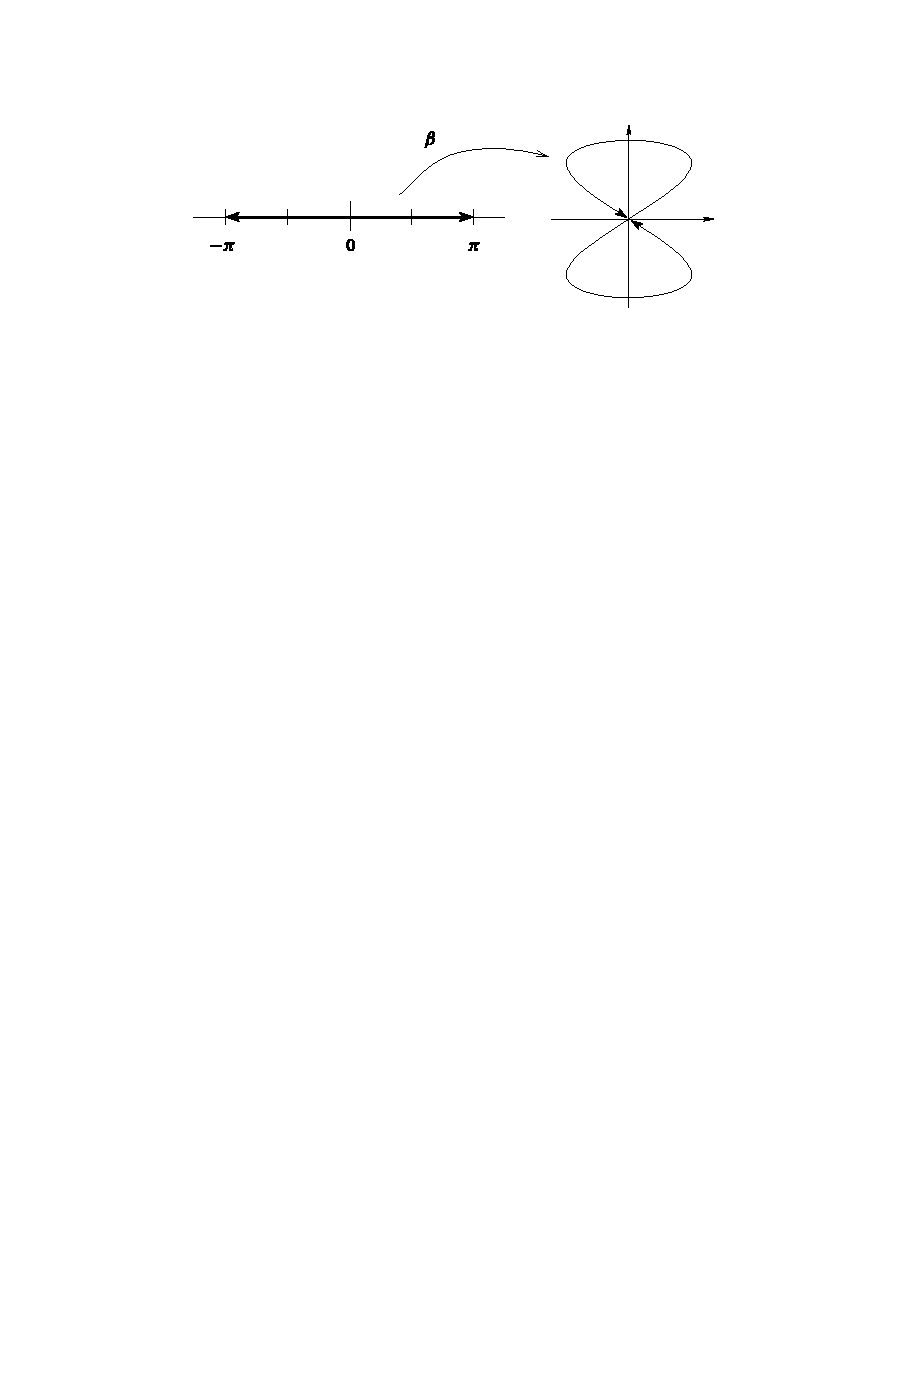
\includegraphics{Images/immersion.pdf}
    \caption{The figure-eight curve $\beta:(-\pi,\pi)\to \bbR^2$ given by $\beta(t)=(\sin 2t,\sin t)$ is an immersion but not an embedding. Its domain is open but its image is closed.}
    \label{fig:immersion}
\end{figure}

As we described above, immersions are maps with injective differentials. Immersions themselves don't need to be injective, and even if they are, their images, as topological subspaces of the codomain, are not even always homeomorphic to the domain. For example, the map in Figure~\ref{fig:immersion} is an immersion whose image is not homeomorphic to the domain. Maps that do respect subspace topology in this way are called embeddings.

In the topological category, the situation is different. A topological immersion is the intuitive analog of the smooth immersion: the injectivity of differentials is replaced by a local homeomorphism property on the domain. 

\begin{defn}[Topological immersion]\index{Immersion!topological}
    A continuous map $f:X\to Y$ is called a topological immersion if for every $x\in X$ there is an open neighborhood $U\subset X$ of $x$ such that $\restr{f}{U}\to f(U)$ is a homeomorphism, where $f(U)$ is taken to have the subspace topology inherited from $Y$.
\end{defn}

A topological embedding then is a global version of a topological immersion: the entire map has to be a homeomorphism onto the image. In particular, it has to be injective.

\begin{defn}[Topological embedding]\index{Embedding!topological}
A topological embedding is a continuous map $f:X\to Y$ that is a homeomorphism onto its image (where the image $f(X)\subset Y$ is taken to have the subspace topology in the target). In other words, it is an injective map such that the topology on the domain must coincide with the initial topology induced by the map.
\end{defn}


In this way the concept of a topological embedding map is dual to that of a topological quotient maps. In the smooth category the picture is a bit different. First, the intuitive smooth version of a quotient map is a smooth submersion that is a topological quotient map. However, as we will see in Section~\ref{sec: submersions}, every smooth submersion is automatically a quotient map, so the second requirement can be dropped. On the other hand, smooth immersions are not always topological embeddings (although they are topological immersions). This is why smooth submersions and smooth immersions are not dual concepts, but instead the concept dual to smooth submersions is the following concept of a smooth embedding.

\begin{defn}[Smooth embedding]\index{Embedding!smooth}
A smooth embedding is a smooth immersion that is topological embedding.
\end{defn}

\begin{example}
\begin{enumerate}
    \item Much like the example in Figure~\ref{fig:immersion}, the mapping of $\bbS^1$ onto a figure eight in $\bbR^2$ can be represented by a parametric map $f(t)=(f_x(t),f_y(t))$. It is an immersion provided that $f'(t)$ doesn't vanish anywhere. However, it is not an embedding because the image (figure eight) is not homeomorphic to the circle.
    \item Excluding the one point on the circle that is mapped to the center point of the figure eight in the last example, we obtain a map $f:(0,1)\to \bbR^2$ whose image is still the whole figure eight. This is an injective immersion. However, it is still not an embedding because the image is compact in the subspace topology, whereas the open interval is not a compact space.
    \item $\gamma:\bbR \to \bbT^2$ given by $\gamma(t)=(\rme^{2\pi\rmi t},\rme^{2\pi\rmi \alpha t})$ for $\alpha\in\bbR \setminus\mathbb{Q}$ is an injective immersion. However, its image is dense in the torus, which means that its subspace topology is very different from that of the real line. Namely, there exist convergent sequences of points in the image whose pre-images don't converge on the real line. This means that $\gamma^{-1}$ is not continuous and $\gamma$ is not an embedding.
    \item The map $f(x)=(0,x^3)$ is a topological embedding $\bbR \hookrightarrow\bbR^2$ but not a smooth embedding because its differential has rank zero at $x=0$. Essentially this restriction insures that smooth structures induced via smooth embeddings coincide with the original ones. The smooth structure induced via $(0,x^3)$ from $\bbR^2$ (with the standard structure) would give one of the non-standard smooth structures on $\bbR $.
\end{enumerate}
\end{example}

\begin{prop}
An injective immersion $f\in C^\infty (M,N)$ is a smooth embedding if any of the following hold:
\begin{enumerate}
    \item $f$ is open or closed;
    \item $f$ is proper;
    \item $M$ is compact;
    \item $\partial M=\varnothing$ and $\dim M=\dim N$.
\end{enumerate}
\end{prop}
\begin{proof}
See \cite[Prop 4.22]{Lee}.
\end{proof}

\begin{thm}[Local embedding theorem]\label{thm.local embedding}
$f\in C^\infty (M,N)$ is an immersion iff it is a local embedding (i.e.\ every point in $M$ has a neighborhood on which the restriction of $f$ becomes an embedding). 
\end{thm}
\begin{proof}
See \cite[Thm 4.25]{Lee}.
\end{proof}

\begin{comment}
\PRLsep
\begin{center}
  {\red Lecture 6 on 15 Dec 2018 ended here}
\end{center}
\end{comment}



\subsection{Submanifolds}
Immersions and embeddings give rise to the notions of immersed and embedded submanifolds.

\begin{defn}\index{Submanifold!immersed}\index{Submanifold!embedded}\index{Submanifold!weakly embedded}\index{Submanifold!initial}\index{Submanifold!properly embedded}
Let $S$ and $M$ be smooth manifolds and let $i:S\to M$ be a continuous map. This triple $S\overset{i}{\to}M$ is called:\index{Submanifold}
\begin{enumerate}
    \item an immersed submanifold if $i$ is a smooth immersion. We write $S<M$.
    \item  a weakly embedded submanifold, or \emph{initial}, if it is immersed and every smooth map $f:N\to M$ such that $\im f\subset S$ restricts in the codomain to a smooth map $f:N\to S$.
    \item an embedded submanifold if $i$ is a smooth embedding map. Often $S\subset M$ with the subspace topology. Then $i$ is required to be a only a topological embedding (and a smooth structure on $S$ can be induced via $i$). We write $S\sub M$.
    \item a properly embedded submanifold if $i$ is a proper smooth embedding map. We write $S\sube M$.
\end{enumerate}
The codimension \index{Codimension} of a submanifold is defined as $\codim S=\dim M -\dim S$.
\end{defn}

Note that sometimes immersed ``submanifolds'' are defined as images of arbitrary immersions, but we avoid that definition since such subsets generally don't admit any manifold structure (since they can self-intersect).

\begin{example}\label{example submanifolds}
\begin{enumerate}
    \item Any open subset is a codimension zero embedded submanifold.
    \item If $F:M\to N$ is an embedding, then $F(M)\sub N$ in the subset sense. i.e.\ embedded submanifolds inside $N$ are exactly the images of embedding maps.
    \item If $S\sub M$ as a subset, then $S$ is closed iff $S\sube M$.
    \item If $S\sub M$ and $S$ is compact, then $S\sube M$.
    \item  The figure eight immersion $t\mapsto (\sin 2t,\sin t)$ is a weak embedding but not an embedding.
    \item If $f\in C^\infty(N,M)$, then its graph $\mathrm{graph}(f)\subset N\times M$ is an embedded submanifold.
\end{enumerate}
\end{example}


\begin{prop}[{{\cite[Prop.~5.18]{Lee}}}]\label{prop 5.18 Lee}
    If $F:M\to N$ is an injective smooth immersion, then $F(M)$ has a unique topology and smooth structure such that it is a smooth submanifold of $N$ and such that $F:M\to F(M)$ is a diffeomorphism onto its image.
\end{prop}
\begin{proof}
    The topology and smooth structure on $F(M)$ are induced by $F$ itself (i.e.~$U\subset N$ is open iff $F^{-1}(U)\subset M$ is open, and the charts on $F(M)$ are $(F(U),\varphi\circ F^{-1})$ for every chart $(U,\varphi)$ on $M$), and they obviously turn $F$ into a diffeomorphism onto its image, and these are the only topology and smooth structure with this property. The inclusion $F(M)\hookrightarrow N$ can be written as a composition $F(M)\overset{F^{-1}}{\to}M\overset{F}{\to}N$. As a composition of a diffeomorphism and a smooth immersion, it is a smooth immersion.
\end{proof}


\begin{prop}
A subset $S\subset M$ is an embedded submanifold iff every point $p\in S$ has a local \emph{``slice chart''}, that is, a local chart map $\varphi$ on a neighborhood $U_p\subset M$  such that its image is a slice ball: $\varphi(S\cap U_p)=\{(x^1,\ldots,x^k,0,\ldots,0)\}$, where $k$ is a fixed number called the dimension of $S$. In particular, given the existence of slice charts, there is a unique smooth structure on $S$ (given by a codomain restriction of the slice atlas) compatible with the subset topology such that $S\sub M$.
\end{prop}
\begin{proof}
It suffices to check that slice charts, whose existence was proved above, form a smooth atlas on $S$. This also proves that, given a topologically embedded submanifold $S$ in a smooth manifold $M$, one can induce a smooth structure on $S$, essentially by defining the slice atlas. See all details in \cite[Thm 5.8]{Lee}. 
\end{proof}


\begin{cor}
$\partial M$ has slice charts by definition, therefore it is an embedded submanifold.
\end{cor}

\begin{prop}
An embedded submanifold  $S\subset M$ is properly embedded iff it is a closed subset of $M$.
\end{prop}
\begin{proof}
Exercise.
\end{proof}

\begin{thm}[Level Set Theorem]\index{Theorem!Level set}\label{thm level set submanifold}
    If $f\in C^\infty(M,N)$ has constant rank $r$ then the level set $f^{-1}(q)$ for any $q\in N$ is a properly embedded codimension $r$ submanifold.
\end{thm}
\begin{proof}
    By definition of rank, there are coordinates in which the local representative is $\wh{f}(x^1,\ldots,x^m)=(x^1,\ldots,x^r,0,\ldots,0)$. Therefore, assuming $q$ is the origin of its coordinate system, $f^{-1}(q)=(0,\ldots,0,\underbrace{y^1,\ldots,y^{m-k}}_{\text{arbitrary}})$. This means that $f^{-1}(q)$ is a local ball slice and therefore an embedded submanifold. It is closed as a pre-image of a closed set under a continuous map, and therefore properly embedded.
\end{proof}
\begin{cor}
Each level set of a smooth submersion $f:M\to N$ is properly embedded and of dimension $\dim N$.
\end{cor}
\begin{cor}[Regular level set theorem]
Every regular level set (i.e.\ level set of a regular value) of a smooth map $f:M\to N$ is a properly embedded submanifold of codimension $\dim N$.
\end{cor}
\begin{proof}
Since the set of all regular points, being the set of points where $f_{\ast}$ has maximal rank, is open (Proposition \ref{domain of maximal rank}), the level set is contained in it together with an open neighborhood $U$ of itself: $f^{-1}(q)\subset U\subset M$. Then $\restr{f}{U}$ is a smooth submersion and we can use the last Corollary.
\end{proof}

\begin{prop}
\begin{enumerate}
    \item All embedded submanifolds $S\subset M$ have local defining functions, i.e.\ $\varphi:C^\infty((U\subset M, \bbR )$ such that $\varphi^{-1}(0)=S\cap U$.
    \item An immersion is a local embedding (i.e.\ its restriction to a sufficiently small neighborhood $U\subset S$ of a point $p\in S$ is an embedding\tablefootnote{Not true for sufficiently small neighborhoods $V\subset M$ of $p\in S\subset M$ that the restriction of the immersion to $S\cap V$ becomes an embedding!}).
\end{enumerate}
\end{prop}
\begin{proof}
\begin{enumerate}
    \item Take a local slice chart such that $\restr{S}{U}=\{(x^1,\ldots,x^k,0,\ldots,0)\}$ and define $\varphi=(x^{k+1})^2+\cdots+(x^m)^2$.
    \item By Theorem \ref{thm.local embedding}.
\end{enumerate}
\end{proof}

\begin{thm}[Extensions of functions]
\begin{enumerate}
    \item If $S\sub M$ as a subset, then any $f\in C^\infty(S)$ can be extended to a $\wt f\in C^\infty(U)$ for some open neighborhood $S\subset U\subset M$ (possibly $U=S$).
    \item If in the above, $S\sube M$, then there is extension to the whole $M$.
\end{enumerate}
\end{thm}
\begin{proof}
\begin{enumerate}
    \item These extensions are possible locally because they are possible in $\bbR^n$ (extensions off a coordinate ball slice; no extension needed if the dimension of the slice is $n$). Then we use a \gls{pou} to glue them together around $S$ much like in Theorem \ref{extension lemma}.
    \item In this case we can just refer to the extension lemma \ref{extension lemma} for closed subsets since any properly embedded manifold is a closed subset in $M$.
\end{enumerate}
\end{proof}

\begin{xca}
Show that the two parts of the last theorem are in fact sufficient, i.e.\ they are criteria for $S$ being embedded or properly embedded, respectively.
\end{xca}

\begin{thm}[Restrictions of functions {{\cite[Thms.~5.27-28]{Lee}}}]\label{thm 5.27 Lee}\label{thm restrictions to submfds}
Let $S< M$ as a subset and $f\in C^\infty(M,N)$. Then:
\begin{enumerate}
    \item the restriction $\restr{f}{S}:S\to N$ is smooth;
    \item if $K<N$, $f(M)\subset K$, and $f$ is continuous as a map $M\to K$, then the codomain restriction $\restr{f}{}^{K}:S\to K$ is also smooth.
    \item if $K\sub N$ and $f(S)\subset K$, then the double restriction $\restr{f}{S}^{K}:S\to K$ is also smooth.
\end{enumerate}
\end{thm}
\begin{proof}
The idea is to show that $\restr{f}{S}=f\circ i$, where $i:S\hookrightarrow M$ is the smooth inclusion map. This is smooth by virtue of being a composition of smooth maps.

For the rest, see the proof in \cite[Thms.~5.27-30]{Lee}.
\end{proof}

Note that to be able to restrict a smooth map in range to an immersed manifold $S$, we need it to be continuous as a map to $S$ with respect to the subspace topology on $S$. Immersed submanifolds which allow for restrictions of smooth maps in range without any such restrictions are exactly the weakly embedded ones.

\begin{rem}
    The terminology around submanifolds is quite confusing and generally only the concept of embedded submanifolds is consistent across different authors. Our use of the term `immersed submanifold' (meaning an image of a smooth injective immersion) is consistent with \cite{Lee}. As indicated in Theorem~\ref{thm 5.27 Lee}, a closely related concept is that of weakly embedded (as in \cite{Lee}), or initial (as in \cite{RS1}), submanifolds. The definition of weakly embedded submanifolds can be thought of as a universal property, and as we've shown above, every embedded submanifold is weakly embedded, however the converse is not true. In other words, we have the following strict inclusions:
    \[\text{Proper embeddings}\subset \text{Embeddings}\subset\text{Weak embeddings}\subset\text{Immersions}.\]
\end{rem}

\begin{thm}[{{\cite[Thm.~5.31]{Lee}}}]\label{thm 5.31 Lee}
    If $S\sub M$ is embedded, then the subspace topology on $S$ and the smooth structure defined by slice charts are the only topology and smooth structure with respect to which $S$ is an embedded or even immersed manifold.
\end{thm}

\begin{thm}[{{\cite[Thm.~5.32]{Lee}}}]\label{thm 5.32 Lee}
    If $S< M$ is immersed, then for a given topology on $S$ there is only one smooth structure making $S$ into an immersed submanifold.
\end{thm}

It is certainly possible for a given subset of $M$ to have more than one topology making it into an immersed submanifold. However, for weakly embedded submanifolds we have a stronger uniqueness result.

\begin{thm}[{{\cite[Thm.~5.33]{Lee}}}]\label{thm 5.33 Lee}
    If $S\subset M$ is a weakly embedded submanifold, then $S$ has only one topology and smooth structure with respect to which it is an immersed submanifold.
\end{thm}


\begin{xca}
\begin{enumerate}
    \item Show $\partial f^{-1}(q)=f^{-1}(q)\cap \partial M$ for any $f\in C^\infty(M,N)$ and $q\in N$ that is a regular value for both $f$ and $\restr{f}{\partial M}$.
    \item Give an example of an immersion $S<M$ and a function $f\in C^\infty(M)$ such that the restriction $\restr{f}{S}$ is not smooth.
\end{enumerate}

\end{xca}




\subsection{Submersions}\label{sec: submersions}

Recall that a split epimorphism is an epi that has a ``right inverse'', or a section/coretraction. In the category $\mathsf{Man}^\infty$, epimorphisms are exactly the smooth maps whose images are dense in the target. Split epimorphisms, however, have to be truly surjective.

\begin{defn}[Local section]\index{Section}
A local section of a continuous (or smooth) map $\pi:M\to N$ is a continuous (resp.~smooth) map $\sigma :U\to M$ defined on an open set $U\subset N$ such that $\pi\circ\sigma =\id_U$.
\end{defn}

This allows us to introduce a topological version of submersions. It looks drastically different from the definition in the smooth case.

\begin{defn}[Topological submersion]\index{Submersion!topological}
    A continuous map $f:X\to Y$ is called a topological submersion if for every $x\in X$ there exists an open neighborhood $V\subset Y$ of $f(x)$ and a local section $\sigma_V:V\to X$ of $f$ that contains $x$ in its image, i.e.~$x\in \sigma(V)$ and $f\circ\sigma=\id_V$. 
\end{defn}

An alternative way to define topological submersions would be to read the Rank Theorem~\ref{Rank thm} (also known as the Local Submersion Theorem in the special case of submersions) combined with our definition of rank (Def.~\ref{def.rank}) to write down a topological characterization of submersions: around every point $x\in X$ there is a neighborhood $U\subset X$ of $x$ and a neighborhood $V\subset Y$ of $f(x)$ and a homeomorphism $\phi:U\to V\times Z$ with some space $Z$ such that $f$ is locally equivalent to the projection onto the first component of $V\times Z$, i.e.~$\restr{f}{U}=\pr_1\circ \phi$. This definition turns out to be a special case of the one given above.

We will now show that smooth submersions are the exact analog of topological submersions: a smooth map is a submersion iff each point in the domain admits a smooth local section through it.

\begin{thm}[Local Section Theorem {{\cite[Thm.~4.26]{Lee}}}]\index{Theorem!Local Section}\label{thm: local section}
    $\pi\in C^\infty(M,N)$ is a submersion iff every $p\in M$ lies in the image of a smooth local section of $\pi$.
\end{thm}
\begin{proof}
    For the forward direction, we have in some local coordinates $f_{\alpha\beta}(x^1,\ldots,x^m)=(x^1,\ldots,x^n)$, where we assume that $p$ is the origin of the coordinate system. Therefore the map locally defined by $\sigma_{\alpha\beta}(y^1,\ldots,y^n)=(y^1,\ldots,y^n,0,\ldots,0)$ is indeed a local section and its image passes through $p$.
    
    For the backward direction, let $p\in M$ and find a local section $\sigma$ such that $p\in \sigma(U)$. Then $p=\sigma(q)$ for some $q\in N$ and $\pi\circ\sigma=\id_U$. Therefore, by taking the differential, $\pi_{\ast p} \sigma_{\ast q}=\id_{T_q N}$, which implies that $\pi_\ast$ is surjective.
    \end{proof}
    
    Next we would like to find the smooth analog for the concept of a quotient map. Recall that a \emph{topological quotient map} is a surjective, strongly continuous map (i.e.\ $V$ is open iff $f^{-1}(V)$ is open). Openness implies strong continuity, thus open surjective maps are necessarily quotient maps, but not every topological quotient map is open (e.g.\ the gluing $\bbD^n\slash \partial \bbD^n$ of the boundary of a ball that gives a sphere is not open). In fact, a surjective continuous map $q$ is a quotient map iff it takes open sets that are unions of fibers of $q$ to open sets. However, these subtleties turns out to be irrelevant in the smooth case as the natural smooth analogs of surjective continuous maps, \emph{submersions}, turn out to be open by the following proposition.
    
    \begin{prop}\label{thm submersions are open quotient maps}
    Any smooth surjective submersion is an open topological quotient map.
    \end{prop}
\begin{proof}
Call the map in question $\pi$. Let $W\mathring{\subset} M$ be an open set and $p\in W$. Pick a local section $\sigma $ passing through $p$, and pick a point $y\in \sigma^{-1}(W)$. Then $y=\pi\circ\sigma(y)\in\pi(W)$. Therefore $\sigma^{-1}(W)$ is an open neighborhood of $\pi(p)$ contained inside $\pi(W)$. Since $\pi(p)$ can be any point in $\pi(W)$, this means that $\pi(W)$ is open, making $\pi$ an open map.

We have thus proved that a smooth submersion is open. A surjective submersion is then a topological quotient map.
\end{proof}

This result motivates the definition of quotient maps in the smooth category $\mathsf{Man}^\infty$. Namely, we only need to require the submersion property (i.e.\ ``infinitesimal surjectivity'') on top of simple surjectivity. By the above result, there is no need to require them to be topological quotient maps.

\begin{defn}[Smooth quotient map]\index{Quotient map!in smooth category}
A \emph{smooth} quotient map is a surjective submersion.
\end{defn}

We have shown that smooth submersions are always open (unlike topological ones). Thus, given a smooth submersion $f:M\to N$, we know that $f(M)$ is open in $N$ and thus an embedded submanifold. Hence we can safely restrict $f$ in its range and obtain a smooth quotient map. With this remark, \emph{smooth submersions and smooth quotient maps are functionally the same thing}.

\begin{rem}
    $\pi\in C^\infty(M,N)$ is a smooth quotient map iff it is a topological quotient map and the given topology and smooth structure on $N$ are the unique ones that make $\pi$ into a smooth submersion. See \cite[Problem 4-7]{Lee}.
\end{rem}

What we have learned can be summarized in the following table, with the lower right cell being a teaser of what's to come.

\begin{center}
\begin{tabular}{ccc}
    & \emph{Injective version} & \emph{Surjective version} \\
    \toprule
    \emph{Basic version} & Immersion & Submersion  \\
    \midrule
    \emph{Stronger version}  & Injective Immersion & Surjective Submersion (a.k.a.~Quotient Map) \\
    \midrule
    \emph{Strongest version}  & Embedding & Fiber Bundle \\
    \bottomrule
\end{tabular}
\end{center}
 
 This table also indicates two possible directions a course in differential geometry can take. The theory of embedding maps (including Whitney's and Nash's embedding theorems, among many others) is fairly sophisticated, and so is the theory of fiber bundles. However, we will mostly follow the ``submersion route'' due to its direct physical relevance.



\newpage

\section{Covering spaces}

\subsection{Homotopy lifting}

A very special type of a submersion is a covering map (which, as we will see, is a special case of a fiber bundle). It turns out that the smooth structure doesn't add anything to the study of these objects, so we will work in the category of topological spaces. The content of this section, with minor additions, is borrowed from the famous book by Bredon \cite{Bredon}, however we can also recommend \cite[Ch. 11]{LeeTop} for a quicker treatment of the case of topological manifolds.


\begin{defn}[Topological covering map]\index{Covering map!topological}
A continuous map $E\overset{\pi}{\to} M$, where $E$ is called the \emph{total space}\index{Total space}, $M$ the \emph{base space}\index{Base space} and $\pi$ the projection, is a \emph{topological} covering map if it is surjective and every $m\in M$ has an open neighborhood $U$ such that $\pi^{-1}(U)$ consists of at most countably many connected components $\wt{U}_i$ and each restriction $\restr{\pi}{\wt{U}_i}:\wt{U}_i\to U$ is a homeomorphism. Such $U_i$ are called \emph{elementary} or \emph{evenly covered}, and we say that $\pi$ is \emph{trivial} over $U_i$. The pre-image $\pi^{-1}(m)$ of a point in the base is called the \emph{fiber above} $m$\index{Fiber}.
\end{defn}

\begin{defn}[Smooth covering map]\index{Covering map!smooth}
A smooth map $E\overset{\pi}{\to} M$ between smooth manifolds $E$ and $M$ is a \emph{smooth} covering map if it is a topological covering map and each restriction $\restr{\pi}{\wt{U}_i}$ is a diffeomorphism.
\end{defn}

In other words, the total space $E$ is locally isomorphic to parts of $M$, but the pre-image of an open set in $M$ can consist of countably many copies of itself embedded in $E$.

\begin{prop}The following properties hold for any smooth covering map $\pi$.
\begin{enumerate}
    \item The neighborhood $U$ whose existence is required in the definition has to be connected.
    \item Covering maps are local diffeomorphisms, submersions, open maps, and quotient maps.
    \item If $\pi $ is injective then it is diffeo.
    \item For $p\in \pi^{-1}(q)$ and $U$ a neighborhood of $q$ as in the definition, there is a unique local section $\sigma:U\to E$ of $\pi$ such that $\sigma(q)=p$.
\end{enumerate}
\end{prop}
\begin{proof}
\begin{enumerate}
    \item Obvious because every connected component of the pre-image can't be diffeomorphic to a disconnected $U$.
    \item Obviously a local diffeo. Submersion because local diffeo. Open for the same reason (or because a submersion). Quotient because surjective and submersion.
    \item If $\pi$ is injective, it's an immersion by the Global Rank Theorem \ref{Global rank}. A map that is an immersion and a submersion is a diffeo.
    \item A section is guaranteed by definition. Just let $\wt{U}$ be the connected component of $\pi^{-1}(U)$ that contains $p$. Then $\restr{\pi}{\wt{U}}$ is a diffeomorphism whose inverse is obviously a section passing through $p$ defined on $U$. Now, suppose there is another section $\sigma':U\to E$ with the same properties. Then $\sigma'(U)\subset \wt{U}$ since $U$ is connected and $\sigma'(q)=p$. But then both $\sigma$ and $\sigma'$ are right inverses to the bijective map $\restr{\pi}{\wt{U}}$, so they have to coincide.
\end{enumerate}
\end{proof}

For now we consider arbitrary covering spaces, not just smooth ones.

\begin{lem}[Lebesque Lemma]\index{Lemma!Lebesque}\label{Lebesque lemma}
    Let $X$ be a compact metric space and let $\{U_\alpha\}_\alpha$ be an open covering of $X$. Then there exists a constant $ \delta >0$ such that any subset $A\subset X$ of diameter $\mathrm{diam} (A)<\delta$ is contained in $U_\alpha$ for some $\alpha$.
\end{lem}
\begin{proof}
    For each $x\in X$ there is an $r(x)>0$ such that the ball $B_{2r(x)}(x)$ is contained inside $U_\alpha$ for some $\alpha$. Then by compactness $X$ is covered by a finite number of the balls $B_{r(x)}(x)$, say for $x=x_1,\ldots,x_n$. Define $\delta=\min \{r(x_i)\mid i=1,\ldots,n\}$. Now if $\mathrm{diam} (A)<\delta$, then there is an $i$ such that $\mathrm{dist}(A,x_i)<r(x_i)$. Since $\mathrm{diam}(A)<\delta\leq r(x_i)$, by the triangle inequality $\mathrm{dist}(a,x_i)<2r(x_i)$. Thus $A\subset B_{2r(x_i)}(x_i)\subset U_\alpha$ for some $\alpha$.
\end{proof}
\begin{lem}[{{\cite[Lem.~3.2]{Bredon}}}]\label{Lemma 3.2 Bredon}
    Let $W$ be a topological space and let $\{U_\alpha\}_\alpha$ be an open covering of $W\times I$ (where $I=[0,1]$).  Then for any $w\in W$ there is a neighborhood $N\subset W$ of $w$ and a positive integer $n$ such that $N\times [i/n, (i+1)/n]\subset U_\alpha$ for some $\alpha$, for each $0\leq i <n$.
\end{lem}
\begin{proof}
    $\{w\}\times I$ can be covered by a finite refinement of $\{U_\alpha\}_\alpha$ of the form $\{N_i\times V_i\}_i$ by compactness of $I$. The Lebesque Lemma~\ref{Lebesque lemma} implies the existence of $n$ such that $[i/n,(i+1)/n]$ is contained in one of the $V_j$. Now take $N=\bigcap_i N_i$.
\end{proof}

\begin{thm}[Path Lifting Property]\index{Path lifting property}\label{Path lifting property}\index{Path Lifting Property}
Consider a topological covering space $E\overset{\pi}{\to}M$ and let $\gamma:[0,1]\to M$ be a path in $M$. Given a point $p$ in the fiber above $\gamma(0)$, there is a unique path $\wt{\gamma}:[0,1]\to E$ such that $\wt{\gamma}(0)=p$ and $\pi\circ\wt{\gamma}=\gamma$. We call $\wt{\gamma}$ the \emph{lift} of $\gamma$ based at $p$.\index{Lift of a path}
\end{thm}
\begin{proof}
By the Lebesque Lemma, there is an $n$ such that each $\gamma([i/n,(i+1)/n])$ lies in an elementary set. Then we can lift by induction in $i$ on each elementary set using the local homeomorphism. At each stage of the induction, the list is already defined at the left-hand endpoint, leading to uniqueness since it singles out a connected component in the pre-image of the elementary set.
\end{proof}
This property is a characteristic property of covering maps and is key in many applications of this theory, such as complex analysis, where the Riemann surfaces of analytic functions are obtained via analytic continuation along paths in the complex plane. The uniqueness of analytic continuation is what guarantees the existence of such a covering map. In fact, the lifting property can be used to define the notion of a covering map.

Now we show the more general form of the lifting property.
\begin{thm}[Covering Homotopy Property/Homotopy Lifting Property]\index{Homotopy Lifting Property}\index{Covering Homotopy Property}\label{homotopy lifting property}
    Given a covering space $\pi :E\to M$, a locally connected space $W$, a homotopy $F :W\times I\to M$, and a map $\wt{f}_0:W\to E$ lifting $f_0=F(\cdot ,0)$, there exists a unique homotopy $\wt{F}_t: W\times I\to E$ of $\wt{f}_0$ that lifts $F$.
\end{thm}
\begin{proof}
    Define $\wt{F}$ on each $\{w\}\times I$ as the unique lifting of a path from Theorem~\ref{Path lifting property}. Now we need to show continuity in $w$. By Lemma~\ref{Lemma 3.2 Bredon} we can find a connected neighborhood $N$ of $w$ in $W$ and an integer $n$ so that $F(N\times [i/n,(i+1)/n])$ is in some elementary set $U_i$. Assuming that $\wt{F}$ is continuous on $N\times \{i/n\}$ we see that $\wt{F}(N\times\{i/n\})$, being connected, must be contained in a  single connected component, say $V$ of $\pi^{-1}(U_i)$. But then on $N\times[i/n,(i+1)/n]$, the lifting $\wt{F}$ must be $F$ composed with the inverse of the homeomorphism $\restr{\pi}{V}:V\to U_i$ (again using connectivity). But this means that $\wt{F}$ is continuous on all of $N\times [i/n,(i+1)/n]$. A finite induction then shows that $\wt{F}$ is continuous on each $N\times I$, and hence everywhere.
\end{proof}
\begin{rem}
    With a slight improvement of the proof, the condition of local connectedness for $W$ can be dropped.
\end{rem}

The uniqueness part of this property is special to covering spaces. In topology, \emph{fibrations} $\pi: P\to M$ \index{Fibration} are generally defined as maps that have the homotopy lifting property (but without uniqueness).

\begin{defn}[Relative homotopy]\index{Relative homotopy}
    Let $X,Y$ be a topological spaces and $K\subset X$ a subspace of $X$. Two maps $f_0,f_1:X\to Y$ are said to be homotopic \emph{relative} to $A$ if there exists a homotopy $F:X\times I\to Y$ such that $F(a,t)=f_0(a)=f_1(a)$ is constant along $I$ for each $a\in A$. We say that this is a homotopy ``$\rel A$''. In particular, if $A$ is a point, this is pointed homotopy that we used in defining homotopy groups. If $A=\{0,1\}\subset I$, this introduces the notion of \emph{homotopy of paths with fixed endpoints}.
\end{defn}
\begin{cor}[{{\cite[Cor.~3.7]{Bredon}}}]\label{cor 3.5 Bredon}
    If $\gamma_0\sim \gamma_1$ are two paths homotopic in $M$ and $\wt{\gamma}_0$, $\wt{\gamma}_1$ are their respective lifts in the covering space $\pi:E\to M$, then their endpoints coincide, $\wt{\gamma}_0(1)=\wt{\gamma}_1(1)$, and $\wt{\gamma}_0$ and $\wt{\gamma}_1$ are homotopic with fixed endpoints.
\end{cor}
\begin{cor}
    Let $\pi:E\to M$ be a covering map. If $\gamma$ is a trivial loop (i.e.\ homotopic to a constant loop) in $M$ then any lifting of $\gamma$ to a path in $E$ is also a trivial loop.
\end{cor}

All of these properties of covering maps with respect to homotopies allow us to pass instead to equivalence classes of homotopic paths, which will transform the study of covering spaces as topological objects into the study of their algebraic functors, namely the fundamental group. 
\begin{cor}[{{\cite[Cor.~3.7]{Bredon}}}]\label{cor 3.7 Bredon}
    Let $\pi:E\to M$ be a covering map and $\pi(p_0)=x_0$. Then \[\pi_\ast : \pi_1(E,p_0)\to \pi_1(M,x_0)\] is a monomorphism whose image consists of the classes of loops at $x_0$ in $M$ which lift to loops at $p_0$ in $E$.
\end{cor}
\begin{cor}[Monodromy Theorem]\index{Theorem!Monodromy}\index{Monodromy}
    If $\gamma$ is a loop in $M$ based at $x_0$ which lifts to a loop in $E$ based at $p_0$ then any loop homotopic to $\gamma$ with fixed endpoints also lifts to a loop in $E$ based at $p_0$.  That is, lifting to a loop is a property of the class $[\gamma]\in\pi_1(M,x_0)$.
\end{cor}
\begin{cor}[{{\cite[Cor.~3.9]{Bredon}}}]\label{cor 3.9 Bredon}
    If a Hausdorff, path-connected, and locally path-connected space $M$ has a nontrivial covering space (i.e.\ one which is not just a direct product of $M$ with a discrete space) then $\pi_1(M,x_0)\neq 1$.
\end{cor}
\begin{proof}
    Let $p_0,p_1$ be two points in the fiber above $x_0$ and let $\gamma $ be a path between them. The  $\pi\circ \gamma$ is a loop in $M$ which does not lift to a loop in $E$. Then  by Corollary~\ref{cor 3.7 Bredon} it follows that $[\pi\circ \gamma]\in\pi_1(M,x_0)$ is not in the image of $\pi_1(E,p_0)$ and hence it is a nontrivial element.
\end{proof}

As a consequence of Corollary~\ref{cor 3.9 Bredon} we now know several spaces having nontrivial fundamental groups: the circle, the Klein bottle, and the projective plane. Let us start with the circle.

\begin{defn}[Degree on a circle]\index{Degree}
    Consider the covering space of $\bbS^1$ defined by the exponential map $p:\bbR \to \bbS^1$, $p(t)=\rme^{2\pi\rmi t}$. Let $\gamma :I\to \bbS^1$ be a loop based at $1\in \bbS^1$. Let $\wt\gamma :I\to \bbR $ be a lifting of $\gamma$ such that $\wt\gamma(0)=0$. Then $\wt\gamma(1)=n\in p^{-1}(\{1\})=\bbZ$. By Corollary~\ref{cor 3.5 Bredon}, $n$ depends only on the homotopy class $[\gamma]\in\pi_1(\bbS^1)$. This integer $n$ is called the degree of $\gamma$ and we write $n=\mathrm{deg}(f)$.
\end{defn}
\begin{thm}[Fundamental group of the circle]\label{pi_1 of the circle thm}
    $\mathrm{deg}: \pi_1(\bbS^1)\to \bbZ$ is an isomorphism.
\end{thm}
\begin{proof}
    First we show that $\mathrm{deg}$ is a homomorphism. Given two loops $\beta,\gamma:I\to \bbS^1$ and their lifts $\wt \beta,\wt\gamma$ both starting at $0\in\bbR $, we have $\wt{\beta}(1)=\mathrm{deg}(\beta)=n$ and  $\wt{\gamma}(1)=\mathrm{deg}(\gamma)=m$. Define $\wt{\gamma}'(t)=\wt{\gamma}(t)+n$. Then $\wt{\gamma}'(0)=\wt{\beta}(1)$, so $\wt{\beta}\bullet \wt{\gamma}'$ is defined, covers $\beta\bullet\gamma$, and $\wt{\beta}\bullet \wt{\gamma}'(1)=\wt{\gamma}'(1)=\wt{\gamma}(1)+n=m+n$, as claimed.

    Second, $\mathrm{deg}$ is surjective since a path from $0$ to $n$ in $\bbR $ maps to a loop in $\bbS^1$ of degree $n$ by definition.

    Third, we sow that $\mathrm{deg}$ is a monomorphism by showing its kernel is zero. Suppose $\gamma:I\to \bbS^1$ has degree $0$. Then, for a lifting $\wt\gamma$ we have $\wt\gamma(1)=0=\wt\gamma(0)$ so that $\wt\gamma$ is a loop and represents an element $\wt{\gamma}\in\pi_1(\bbR ,0)=1$, since $\bbR $ is contractible. Thus $[\gamma]=p_\ast([\wt\gamma])=p_\ast (1)=1$.
\end{proof}


\begin{rem}\label{covering spaces and connections}
	The Path Lifting Property is our first example of a \emph{connection}\index{Connection}. A connection is a prescription for lifting curves from the base $M$ into the total space. Alternatively, it is a prescription for lifting vector fields in the base to what is called \emph{horizontal} vector fields in the total space. On covering spaces, as we see, the connection is unique due to the fact that the total space is locally diffeomorphic to the base.
	
	The monodromy (how points in the fiber get permuted after a transport over a curve in the base) is also known as \emph{holonomy}\index{Holonomy} in the context of connections.
\end{rem}


\begin{comment}
    \begin{samepage}
        \PRLsep
        \begin{center}
            {\red Lecture 7 on 11 Jan 2019 ended here}
        \end{center}
    \end{samepage}
\end{comment}

\[
\begin{tikzcd}[every matrix/.append style={name=m}, row sep=large, column sep=large,   
execute at end picture={\draw [<-] ([xshift=-5mm,yshift=0mm]m-2-2.north) arc[start angle=-90,delta angle=-270,radius=0.25cm];}]
   & E\arrow[d,"\pi"]\\
   W \arrow[r,"f", swap] \arrow[ur,"\wt f",dashed] & M
\end{tikzcd}
\]
Aside from homotopies, one can try to lift arbitrary mappings into the base space of a fibration. In general the existence of these liftings is difficult to establish. In the case of covering spaces, however, the answer is quite simple: a map from a space $W$ into $M$ can be lifted into the total space of $\pi:E\to M$ iff the images of all nontrivial loops in $W$ are among those loops in $M$ that can be lifted to $E$, and the lifting is unique. This is formalized in the following Theorem.

\begin{figure}
    \centering
    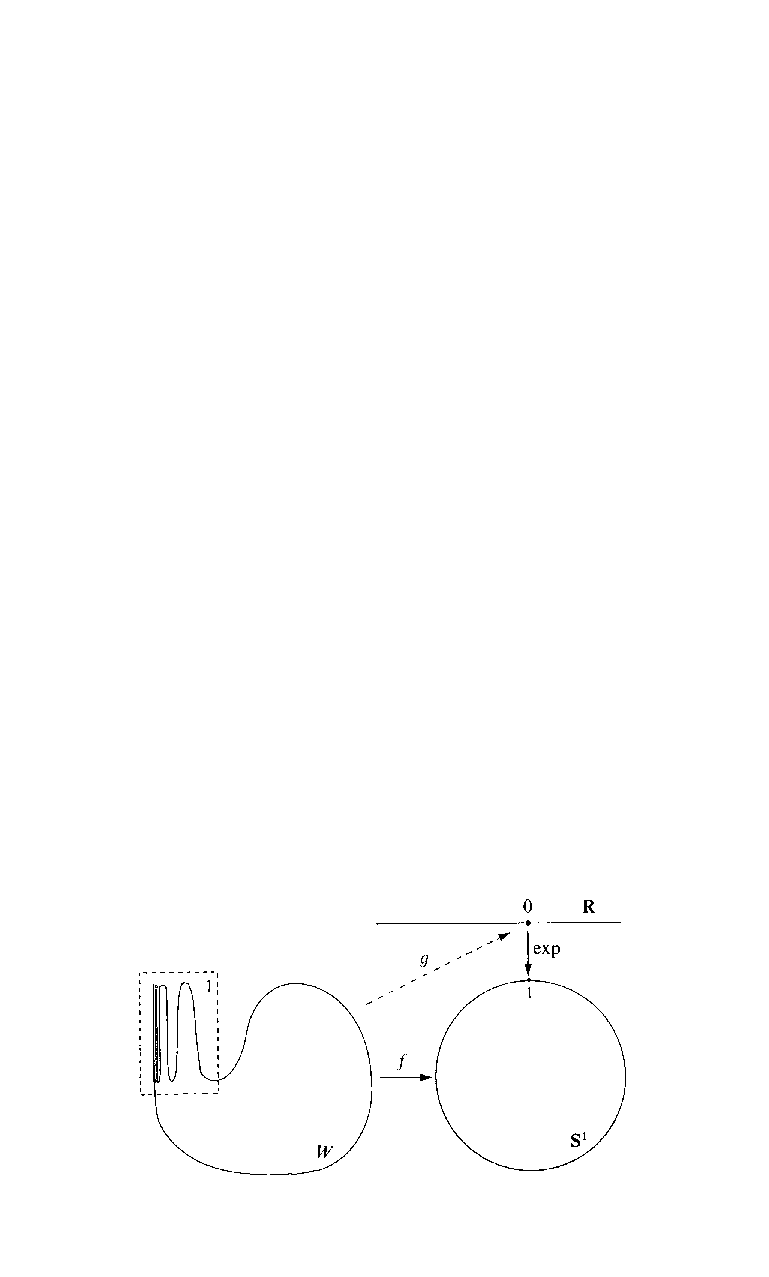
\includegraphics[width=0.7\textwidth]{Images/discont_lift.pdf}
    \caption{The map $f$ here collapses the entire ``$\sin 1/x$'' part of the space on the left into the basepoint $1$ on the circle. If a lifting map $g$ into the real line existed, then the vertical part of the ``$\sin 1/x$'' curve would have to be mapped to $0$, whereas the wiggly part would map to $1$ under $g$, making it discontinuous. From \cite[Fig.~III-6]{Bredon}.}
    \label{fig:discont_lift}
\end{figure}

\begin{thm}[Lifting Theorem]\index{Theorem!Lifting}\label{Lifting Theorem}
    Let $\pi:E\to M$ be a covering map with $\pi (p_0)=x_0$. Assume that $W$ is path-connected and locally path-connected and that $f:W\to M$ is a map with $f(w_0)=x_0$. Then a pointed map $\wt f:(W,w_0)\to (M,x_0)$ such that $\pi\circ\wt{f}=f$ exists iff $f_\ast (\pi_1(W,w_0))\subset \pi_\ast (\pi_1(E,p_0))$. Moreover, $\wt f$ is unique.
\end{thm}
\begin{proof}
    Let us construct $\wt f$ explicitly. Given $w\in W$, let $\lambda:I\to W$ be a path from $w_0$ to $w$. Then $f\circ \lambda$ is a path in $M$. Lift this to a path $\wt\lambda:(I,0)\to (E,x_0)$ and let $\wt{f}(w)=\wt{\lambda}(1)$. Then $\pi\circ \wt{f}(w)=\pi(\wt{\lambda}(1))=f(\lambda(1))=f(w)$.

    To see that $\wt{f}$ is well defined, suppose $\lambda'$ is another path in $W$ from $w_0$ to $w$ and let $\eta=(\lambda ')^{-1}$ be the reverse path from $w$ to $w_0$. Then $\lambda\bullet \eta$ is a loop based at $w_0$, and $(f\circ \lambda)\bullet (f\circ\eta)$ is a loop in $M$ based at $x_0$. Since 
    \[[f\circ\lambda \bullet f\circ\eta]=f_\ast([\lambda\bullet\eta]\in \im(f_\ast)\subset \im(\pi_\ast),\]
    $f\circ\lambda\bullet f\circ\eta$ lifts to a loop in $E$ based at $p_0$. The reverse of the portion of this lifting corresponding to $\eta$ then is a lifting $\wt{\lambda}'$ of $\lambda '$ and $\wt{\lambda}'(1)=\wt{\lambda}(1)$, as required.

    Next, we have to show that $\wt{f}$ is continuous. Let $w\in W$  and put $x=f(w)$. Let $U\subset <$ be an elementary neighborhood of $x$, and by local path-connectedness of $W$ we can let $V$ be a path-connected neighborhood of $w$ such that $f(V)\subset U$. For any point $w'\in V$ we can construct a path from $w_0$ to $w'$ by concatenating a given path $\lambda$ to $w$ with a path $\sigma$ in $V$ from $w$ to $w'$. Since $f(V)$ is contained in an elementary set, the lifting of $f\circ \sigma$ is simply $f\circ\sigma$ composed with the local inverse of $\pi$ that takes $U$ to the component of $\pi^{-1}(U)$ that contains $\wt{f}(w)$. This same component is used for all $w'\in V$ and it follows that $\wt{f}$ is continuous at $w$.

    The converse direction of the theorem follows immediately from $f_\ast=\pi_\ast\circ \wt{f}_\ast$.
\end{proof}
\begin{rem}
    Unlike in the homotopy lifting property (Theorem~\ref{homotopy lifting property}), the condition of local path connectedness for $W$ cannot be dropped here. See an example in Figure~\ref{fig:discont_lift}.
\end{rem}

\begin{cor}[{{\cite[Cor.~4.2]{Bredon}}}]\label{cor 4.2 Bredon}
    Under the conditions of the Lifting Theorem~\ref{Lifting Theorem}, if $W$ is also simply connected, then the lifting $\wt{f}$ always exists and is unique given a basepoint $p_0\in E$.
\end{cor}

\begin{cor}\label{cor homotopy groups of coverings}
    Given a covering space $E\overset{\pi}{\to}M$, there is a natural isomorphism of higher homotopy groups
    \[\pi_n(E,p_0)\cong \pi_n(M,x_0),\; n\geq 2.\]
\end{cor}
\begin{proof}
    Injectivity follows from the uniqueness of the liftings of maps $\bbS^n\to M$ into $E$. Surjectivity follows from the Lifting Theorem~\ref{Lifting Theorem} combined with the fact that $\pi_1(\bbS^n)$ is trivial for $n\geq 2$ (Corollary~\ref{cor pi_1(S^n)=0}).
\end{proof}

\begin{cor}\label{cor: homotopy groups of circle}
    $\pi_n(\bbS^1)=1$ for $n>1$.
\end{cor}
\begin{proof}
    Any map $f:\bbS^n\to \bbS^1$ lifts to $\wt{f}:\bbS^n\to \bbR $ by Corollary~\ref{cor 4.2 Bredon}. But $\wt f$ is homotopically trivial since $\bbR $ is contractible, so $f=\pi\circ\wt{f}$ is also homotopically trivial.
\end{proof}


\subsection{Morphisms of covering spaces}


\begin{defn}[Category of covering spaces]
The category $\mathsf{Cov}_M$ of covering spaces of a given base $M$ (say, topological covering spaces) consists of all covering spaces of $M$. The morphisms between two covering spaces $\pi$ and $\pi'$ are morphisms $f:E\to E'$ that ``map fibers to fibers'', i.e.\ $\pi'\circ f=\pi$, or equivalently if the following triangle commutes:
\[
\begin{tikzcd}[every matrix/.append style={name=m},   
execute at end picture={\draw [<-] ([xshift=0mm,yshift=-2mm]m-2-2.north) arc[start angle=-90,delta angle=-270,radius=0.25cm];}]
   E \arrow[rr,"f"]\arrow[ddr,swap,"\pi"]& & E'\arrow[ddl,"\pi'"]\\
   & \, & \\
   & M & \\
\end{tikzcd}
\]
\end{defn}


\begin{lem}[{{\cite[Lem.~4.4]{Bredon}}}]\label{lem 4.4 Bredon}
    Let $W$ be connected and $E$ be Hausdorff. Let $\pi:E\to M$ be a covering map and $f:W\to M$ a map. Let $\wt{f}_1,\wt{f}_2$ be two liftings of $f$ into $E$. If $\wt{f}_1(w)=\wt{f}_2(w)$ for some point $w\in W$, then $\wt{f}_1\equiv \wt{f}_2$.
\end{lem}
\begin{proof}
    Let $\wt{f}_1(w)=\wt{f}_2(w)=p$. Let $U$ be an elementary open neighborhood of $f(w)$ in $M$. Let $V$ be the component of $\pi^{-1}(U)$ containing $p$. Then $A=\wt{f}_1^{-1}(V)\cap\wt{f}_2^{-1}(V) $ is an open set in $W$ and for $a\in A$ we have $\wt{f}_1(a)=\wt{f}_2(a)$ since the homeomorphism $\pi:V\to U$ maps them both to $f(a)$. This shows that the set $\{w\in W\mid \wt{f}_1(w)=\wt{f}_2(w)\}$ is open. But this set is also closed since it is the inverse image of the diagonal under the map $\wt{f}_1\times \wt{f}_2:W\to E\times E$, and the diagonal is closed since $E$ is Hausdorff. Since $W$ is connected, this set is either empty or all of $W$.
\end{proof}
\begin{cor}[{{\cite[Cor.~4.5]{Bredon}}}]\label{cor 4.5 Bredon}
    Let $\pi_i:E_i\to M$, $i=1,2$, be covering maps such that $E_1$ is simply connected, and let $p_i\in E_i$ be such that $\pi_1(p_1)=\pi_2(p_2)$. Then there is a unique morphism of covering spaces $f:E_1\to E_2$ such that $f(p_1)=p_2$. Moreover, $f$ is a covering map.
\end{cor}
\begin{proof}
    By the Lifting Theorem~\ref{Lifting Theorem}, since $\pi_1(E_1,p_1)=1$, there is a lifting of $\pi_1\to E_1\to M$ to a map $f:E^1\to E^2$ such that $\pi_2\circ f=\pi_1$. It is unique by Lemma~\ref{lem 4.4 Bredon}.  It is an easy exercise to show that $f$ is a covering map.
\end{proof}
\begin{cor}[{{\cite[Cor.~4.6]{Bredon}}}]\label{cor 4.6 Bredon}
    If in Corollary~\ref{cor 4.5 Bredon} both $E_1$ and $E_2$ are simply connected, then the unique map $f$ is a homeomorphism.
\end{cor}
\begin{proof}
    By Corollary~\ref{cor 4.5 Bredon}, in addition to $f$ there is also an analogous map $k:E_2\to E_1$. Then $k\circ f:E_1\to E_1$ covers the identity map at $p_1$. By Lemma~\ref{lem 4.4 Bredon}, it must equal the identity everywhere. Similarly $g\circ k=\mathrm{id}_{E_2}$, hence $k=f^{-1}$.
\end{proof}

This implies that all simply connected covering spaces of a given base space $M$ are isomorphic in the category $\mathsf{Cov}_{\bullet M}$. Such covering spaces are called universal, and are guaranteed to exist under a mild restriction.

\begin{defn}[Locally relatively simply connected space]
    A space $X$ is locally relatively simply connected (or semilocally simply connected) if each point has a neighborhood $U$ such that all loops inside of $U$ are homotopically trivial in $X$ (i.e.\ for any $u\in U$ the homomorphism $\pi_1(U,u)\to \pi_1(X,u)$ is trivial).
\end{defn}


One can show that the existence of a simply connected covering space is equivalent to $M$ being locally relatively simply connected (see~\cite[Theorem~8.4]{Bredon}). Since we are mostly interested in manifolds, we will only prove the existence. Let us only work with connected, locally simply connected spaces (in particular, connected manifolds).

\begin{thm}[Universal cover]\index{Universal cover}
For a given base $M$ that is a connected and \emph{locally relatively simply connected} Hausdorff space, there is a unique (up to homeomorphism) topological covering space $E\overset{\pi}{\to}M$ whose total space $E$ is simply connected. This covering space is denoted by $\wt M$ and is called the \emph{universal cover} of $M$.\index{Universal cover}
\end{thm}
\begin{proof}
See \cite[Thm 11.43]{LeeTop} or \cite[Thm 8.4]{Bredon}. The basic idea is to explicitly construct $\wt M$ as the space of endpoints of all possible paths in $M$ based at a fixed point $m\in M$. Two paths are equivalent if their endpoints coincide and they are homotopic with fixed endpoints. The topology on this set of paths is introduced by considering sets of homotopic paths with endpoints belonging to an open set in $M$ (and the homotopies fix the starting point but can move the endpoint within the open set, see figure). The projection $\pi$ maps a path to its endpoint. It is not difficult to check that this is indeed a topological covering map and the total space is simply connected. Uniqueness will follow from the universal property described below.

\begin{center}
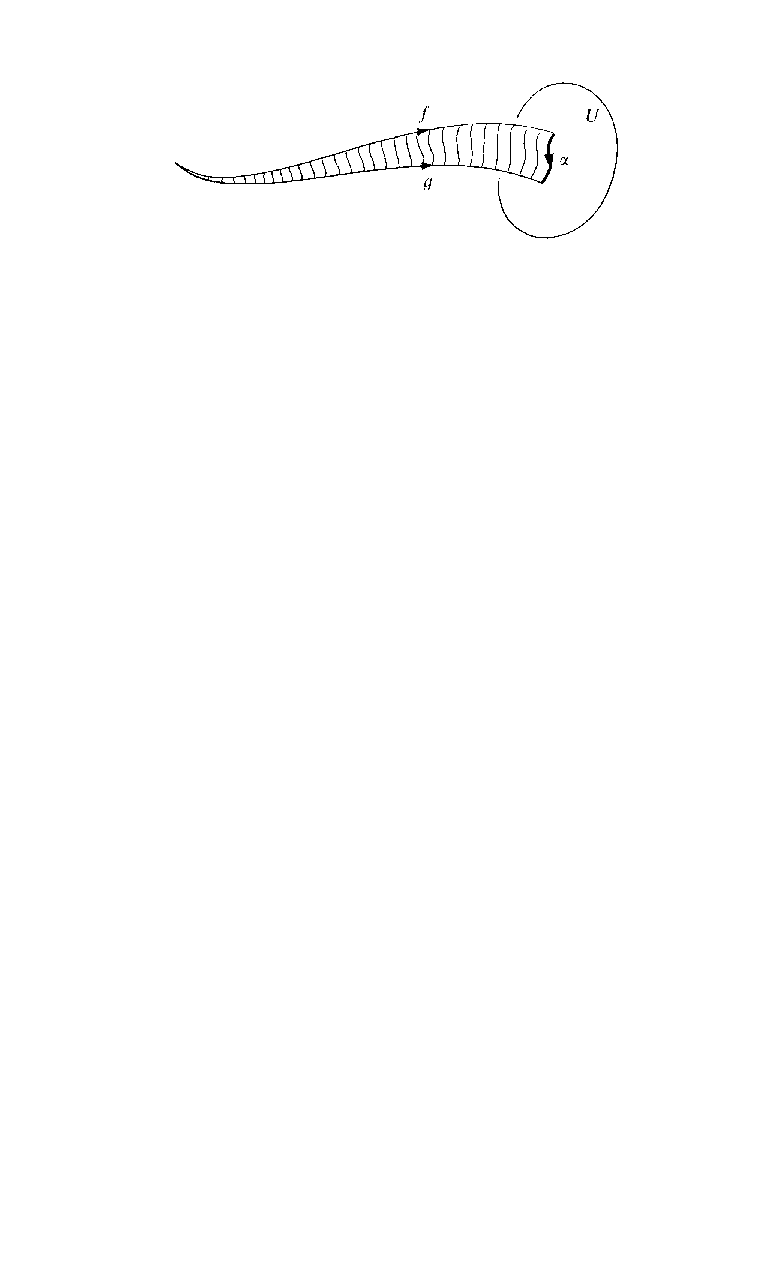
\includegraphics[width=0.5\textwidth]{Images/uni_open_set.pdf}
\end{center}
\end{proof}
\begin{rem}
    By examining the details of the proof one can notice that local simply-connectedness is not actually required, and semilocal simply-connectedness is sufficient. The converse direction is clear: if a loop is in an evenly covered subspace of $M$ then it lifts to $E$, and if $E$ is simply connected, the loop must be trivial in $E$. But then the composition of its homotopy to a constant loop with the covering map $\pi$ shows that the original loop in $M$ must be trivial. Thus we have shown that a connected and locally path-connected $M$ has a universal covering space iff it is locally relatively simply connected.
\end{rem}
\begin{example}
    The Hawaiian earring (Example~\ref{hawaiian earring}), as well as the infinite-dimensional torus $\bbT^\infty=\prod_{i=1}^\infty \bbS^1$, are not locally relatively simply connected, and thus don't have universal coverings.
\end{example}

\begin{thm}
Let $E\overset{\pi}{\to}M$ be a topological covering map and fix a smooth structure on $M$. Then $E$ is a topological manifold that supports a unique smooth structure such that $\pi$ is a smooth covering map with $\pi^{-1}(\partial M)=\partial E$.
\end{thm}
\begin{proof}
See \cite[Prop 4.40]{Lee}.
\end{proof}
This theorem essentially means that in order to classify smooth covering spaces above a smooth base manifold, it suffices to only classify the topological covering spaces, and they are in one-to-one correspondence with the smooth ones. In other words, the theory of covering spaces is an intrinsically topological theory that doesn't gain or lose anything from imposing smooth structures.

\begin{cor}
For a connected smooth manifold $M$, there exists a unique simply connected smooth covering space called the universal covering manifold of $M$.
\end{cor}
From now on we won't really distinguish between smooth and topological covering spaces, although we only care about the smooth case.

Corollaries~\ref{cor 4.5 Bredon} and \ref{cor 4.6 Bredon} can now be restated in terms of morphisms:
\begin{cor}[Universality of the universal cover]\index{Universal property!of universal covers}
    \;
    \begin{enumerate}
       \item Any morphism of covering spaces is itself a covering map;
        \item If $M$ is a topological manifold (or any space that has a universal covering space), then $\wt{M}$ is the initial object in the category $\mathsf{Cov}_{\bullet M}$ of pointed covering spaces of $M$ (i.e.\ objects are $E\overset\pi\to M$ with a basepoint $p_0\in E$ and morphisms must respect the basepoints).
    \end{enumerate}
\end{cor}

In the category of non-pointed covering spaces, the universal cover is not an initial object, but the arrows coming out of it are unique up to automorphisms of the two covering spaces at the ends of the arrow. We now describe the sets of such automorphisms.

\subsection{Deck transformations}

\begin{defn}[Group action]
    An (right/left) action of a group $G$ on a set (or a space, a manifold) $X$ is a map $\Phi: G\times X\to X$, with its partial maps denoted by $\Phi_g=\Phi (g,\_):X\to X$ and $\Phi_x=\Phi(\_,x):G\to X$, such that $\Phi_e=\mathrm{id}_X$ and one of the following:
    \[
        \text{left action}:\quad \Phi_g\circ \Phi_h=\Phi_{gh},\]
        \[\text{right action}: \quad \;\; \Phi_g\circ \Phi_h=\Phi_{hg}.
    \]
    In other words, right actions are the same thing as left actions on the opposite group $G^{\mathrm{op}}$. For this reason right actions are usually written as $x\cdot g=\Phi_g(x)$ and left actions as $g\cdot x=\Phi_g(x)$. The sets $G(x)=\Phi_x(G)$ are called \emph{orbits}.
\end{defn}
In the topological and smooth categories one usually considers continuous or smooth group actions, provided $G$ is a Lie group, but we will delay that discussion until Section~\ref{sec: Lie group actions}. For now $G$ will always be a discrete group (i.e.\ a group with discrete topology), so any condition of continuity or smoothness on the action is simply a condition on each $\Phi_g$ individually.

\begin{defn}[$G$-equivariant maps]\index{Equivariant maps}\index{$G$-Set}
    The category of sets (spaces, manifolds) carrying a (left) action of $G$ is called $G\mathsf{-Set}$. Morphisms in this category are maps $f:X\to Y$ such that for all $g\in G$, $f(g\cdot x)=g\cdot f(x)$. These maps are called $G$-equivariant. Similarly, $G\mathsf{-Set}_\bullet$ consists of pointed sets with equivariant maps that respect basepoints. 
\end{defn}
\begin{defn}[Stabilizer]\index{Stabilizer}
    Given a group $G$ acting on a set $X$, and a point $x\in X$, the stabilizer of $x$ is defined as the subgroup $G_x=\{g\in G\mid \Phi(g,x)=x\}$.
\end{defn}
\begin{defn}[Transitive action]
    An action $\Phi$ is called transitive if it has only one orbit, i.e.\ for each pair $x,y\in X$ there is an $g\in G$ such that $\Phi(g,x)=y$.
\end{defn}
\begin{defn}[Simply transitive action]
    An action $\Phi$ is called simply transitive if for each pair $x,y\in X$ there is a \emph{unique} element $g\in G$ such that $\Phi(g,x)=y$.
\end{defn}
\begin{defn}[Faithful action]
    An action $\Phi$ is called faithful if no nontrivial elements of $G$ act trivially: $\Phi_g=\mathrm{id}_X \Leftrightarrow g=e$.
\end{defn}
\begin{defn}[Free action]
    An action $\Phi$ is called free if no nontrivial elements of $G$ have any fixed points: $\exists\,x\in X: \Phi(g,x)=x\Leftrightarrow g=e$. 
\end{defn}
\begin{prop}
    An action is simply transitive iff it is free and transitive.
\end{prop}
\begin{proof}
    Assume a left action for simplicity. For the necessary condition, we only need to show freeness. If $\Phi_g=\mathrm{id}_X$, then $g\cdot x=x=e\cdot x$, therefore by simple transitivity $g=e$.

    For the converse, assume there are two elements such that $g_1\cdot x=g_2\cdot x=y$. Then $g_2^{-1}g_1\cdot x=x$, which means $g_2^{-1}g_1=e$ by freeness.
\end{proof}

Throughout this section let $E\overset{\pi}{\to}M$ be a covering space with a fixed point $x_0\in M$. For simplicity we also denote
\[G=\pi_1(M,x_0),\quad \quad F=\pi^{-1}(x_0).\]
The discrete set $F$ is called the \emph{fiber} of $\pi$ over $x_0$. We are going to describe an action of the group $G$ on $F$ as a group of permutations. 

Let $p\in F$ and let $g\in G$ be an element represented by a loop $\gamma :I\to M$. Lift it to get a map $\wt{\gamma}$ in $E$ with $\wt{\gamma}(0)=p$. Then define
\[\Phi(g,p)=p\cdot g =\tilde{\gamma}(1) \in F.\]
By Corollary~\ref{cor 3.5 Bredon} this does not depend on the choice of $\gamma$ and thus is a well-defined map $\Phi:F\times G\to F$. Now we can check some properties of this function:
\begin{enumerate}
    \item $x\cdot e=x$.
    \item $(x\cdot g)\cdot h=x\cdot (gh)$, i.e.\ it is a right action (because the product of two loops $gh$ corresponds to the application of $\Phi_g$ and then $\Phi_h$).
    \item $E$ is connected iff this action is transitive (i.e.\ there is only one orbit, $p\cdot G=F$). To see this, pick a path in $E$ from $p_0$ to another $p\in F$. This projects onto a loop $\gamma$ in $M$ and $g=[\gamma]$ provides the required element: $p_0\cdot p=p$. Conversely, if $E$ is not connected, the action is obviously not transitive.
    \item The stabilizer of a point is $G_{p_0}=\{g\in G\mid p_0\cdot g=p_0\}$. Then 
    \[
        \boxed{G_{p_0}=\im \pi_\ast=\pi_\ast(\pi_1(E,p_0))}\label{stabilizer}
    \]
    where $\pi_\ast:\pi_1(E,p_0)\to \pi_1(M,x_0)=G$ is the homomorphism induced by $\pi$. This is true because $g\in G_{x_0}$ iff $g=[\gamma]$ and $\gamma$ lifts to a loop at $p_0$, i.e.\ iff $g\in \im p_\ast$.
    \item Assuming $E$ is connected, the map $\phi: \ _{G_{p_0}}\bslash^{G}\to F$ taking the right coset $G_{x_0}g$ to $p_0\cdot (G_{p_0}g)=p_0\cdot g$ is a bijection.
\end{enumerate}
Obviously any covering space decomposes into a disjoint union of connected components, and the action of $\pi_1(M)$ is transitive on the fiber of each component separately. In what follows, we generally assume that $E$ is connected. In summary, we have the following Theorem.
\begin{thm}
    Given a connected covering space $\pi:E\to M$, there is a one-to-one correspondence between the set $_{\pi_\ast(\pi_1(E,p_0))}\bslash^{\pi_1(M,x_0)}$ of right cosets, and the fiber $\pi^{-1}(x_0)$. (Note that $\pi_\ast(\pi_1(E,p_0))\cong \pi_1(E,p_0)$ since $\pi_\ast$ is a monomorphism by Corollary~\ref{cor 3.7 Bredon}.)
\end{thm}
\begin{cor}
    The number of sheets of a connected covering space equals the index (number of left or right cosets) of $G_{p_0}=\pi_\ast(\pi_1(E,p_0))$ in $G=\pi_1(M,x_0)$.
\end{cor}
\begin{cor}
    If $\wt\pi:\wt M\to M$ is a universal covering map (i.e.\ $\wt M$ is simply connected), then the number of sheets equals the order (cardinality) of the group $\pi_1(M,p_0)$.
\end{cor}

\begin{example}[Fundamental groups of real projective spaces]
    Since $\bbS^n$ is simply connected for $n>1$ and $\bbS^n$ is a double covering of the real projective space $\bbR P^n$, it follows that $\pi_1(\bbR P^n)\cong \bbZ_2$.
\end{example}

\begin{defn}
    For a covering space $E\overset{\pi}{\to}{M}$, define the group $\Aut(\pi)$ of automorphisms of this covering space in the category $\mathsf{Cov}_M$ (also called \emph{deck transformations}\index{Deck transformations}). Its elements are homeomorphisms of $E$ that cover the identity map on $M$. For a given elementary open set $U\subset M$, they permute the connected components $U_i$ of the pre-image $\pi^{-1}(U)$. In other words, the group $\mathrm{Aut}(\pi)$ acts on $E$ via morphisms of covering spaces.
\end{defn}

\begin{prop}[{{\cite[Prop.~6.2]{Bredon}}}]\label{prop 6.2 Bredon}
    If $a\in \Aut(\pi)$ and $g\in\pi_1(M,p_0)$ and $x\in \pi^{-1}(x_0)$ then $a(x)\cdot g=a(x\cdot g)$. In other words, deck transformations are equivariant with respect to the action of $\pi_1(M,x_0)$.
\end{prop}
\begin{proof}
    Let $\gamma$ be a loop at $x_0$ representing $g$ and lift it to a path $\wt\gamma$ starting at $p$. Then $\wt\gamma(1)=p\cdot g$ by definition. Look at the path $a\circ \wt{\gamma}$. It is a lifting of $\gamma$ and starts at $a(p)$. Thus is ends at $a(p)\cdot g$ by definition of the latter. But it also ends at $a(\wt\gamma(1))$, which is $a(p\cdot g)$.
\end{proof}

This proof actually shows that not only automorphisms are $G$-equivariant, but all morphisms in the category $\mathsf{Cov}_M$ are. This means that the action of $\pi_1(M)$ that we've constructed is \emph{natural}. These results can be summarized by the following Theorem.
\begin{thm}[Monodromy Action]\index{Monodromy}
For any covering space $E\overset{\pi}\to M$, 
\begin{enumerate}
    \item there is a natural homomorphism $\pi_1(M)\to \Aut(\pi)$ called the \emph{monodromy action};
    \item $\Aut(\wt \pi)\cong\pi_1(M)$, where $\wt\pi$ is the universal cover.
\end{enumerate}
\end{thm}

\begin{defn}[Normalizer]\index{Normalizer of a subgroup}
For a subset (not necessarily a subgroup) $H\subset G$ of a group $G$, its normalizer is 
\[N_G(H)=\{n\in G\mid nH=Hn\}.\]
A subgroup $H$ is normal in $G$ iff $N_G(H)=G$. Otherwise, $N_G(H)$ is the largest subgroup of $G$ such that $H$ is a normal subgroup of $N_G(H)$.
\end{defn}
\begin{rem}
    If $H$ is a subgroup, then $H\subset N_H(H)$. Moreover, $N_G(g^{-1}Hg)=g^{-1}N_G(H)g$, so the normalizers of conjugate subsets are conjugate.
\end{rem}

The following lemma is the analog of the ``change of coordinates'' formulas in linear algebra: mapping the coordinates of vectors to a new basis is equivalent to conjugating the matrices representing linear operators.
\begin{lem} For any group $G$ acting on a set $X$ from the right,
\[\boxed{G_{p_0\cdot g}=g^{-1}G_{p_0}g.}\label{conjugate stabilizers}\]
Similarly, for left actions, $G_{g\cdot p_0}=gG_{p_0}g^{-1}$.
\end{lem}
\begin{proof}
    \[
        G_{p_0\cdot g}=\{h\mid (p_0\cdot g)\cdot h=p_0\cdot g\}=\{h\mid p_0\cdot ghg^{-1}=p_0\}=\{h\mid ghg^{-1}\in G_{p_0}\},
    \]
\end{proof}

The most important question in the study of deck transformations is: given two points in the fiber, when does there exist a deck transformation mapping one to the other? This is answered in the following theorem.
\begin{thm}[{{\cite[Thm.~6.3]{Bredon}}}]\label{thm 6.3 Bredon}
    Provided $E$ is connected, let $p,p_0\in F=\pi^{-1}(x_0)$, $G=\pi_1(M,x_0)$ and $G_{q}=\pi_\ast(\pi_1(E,q))$ for any $q\in E$. Then \gls{tfae}:
    \begin{enumerate}
        \item $\exists\, a\in \mathrm{Aut}(\pi)$ such that $a(p_0)=p$.
        \item $\exists\, g\in N_G(G_{p_0})$ such that $p_0\cdot g=p$.
        \item $G_{p_0}=G_p$.
    \end{enumerate}
\end{thm}
\begin{proof}
    Recall that $G_{p_0}=\pi_\ast(\pi_1(E,p_0))$ and $G_{p}=\pi_\ast(\pi_1(E,p))$. By the Lifting Theorem~\ref{Lifting Theorem} a map $a$ covering the identity and taking $p_0$ to $p$ exists iff $\pi_\ast(\pi_1(E,p_0))\subset \pi_\ast(\pi_1(E,p))$. Similarly, a map $a'$ covering the identity and mapping $p$ to $p_0$ exists iff the opposite inclusion holds. If both exist then $a\circ a'$ covers the identity and has a point in common with the identity, therefore $a\circ a'=\mathrm{id}_E$ by Lemma~\ref{lem 4.4 Bredon}. This proves the equivalence $(1)\Leftrightarrow (3)$.

    Now we can prove $(2)\Rightarrow(3)$: if $p=p_0\cdot g$ and $g\in N(G_{p_0})$ then $G_p=G_{p_0\cdot g}=g^{-1}G_{p_0}g=G_{p_0}$ as claimed.

    For $(3)\Rightarrow (2)$, suppose $G_{p_0}=G_p$ and $p=p_0\cdot g$ (such a $g$ exists since $G$ acts transitively on $F$). Then $G_{p_0}=G_p=G_{p_0\cdot g}=g^{-1}G_{p_0}g$, so $g\in N(G_{p_0})$.
\end{proof}
From $(2)\Leftrightarrow(1)$ and the last part of the proof we have the following Corollary.
\begin{cor}[{{\cite[Cor.~6.4]{Bredon}}}]\label{cor 6.4 Bredon}
    For a connected covering space, the subgroup $G_{p_0}=\pi_\ast(\pi_1(E,p_0))$ is normal in $G=\pi_1(M,x_0)$ iff the action of $\mathrm{Aut}(\pi)$ is (simply) transitive on $F=\pi^{-1}(x_0)$.
\end{cor}
\begin{cor}[{{\cite[Cor.~6.5]{Bredon}}}]\label{cor 6.5 Bredon}
    In a connected covering space, if $p$ ranges over the fiber $F$ then $G_p$ ranges over all conjugates of $G_{p_0}=\pi_\ast(\pi_1(E,p_0))$.
\end{cor}
\begin{proof}
    This is a consequence of (\ref{conjugate stabilizers}).
\end{proof}

\begin{rem}
    It is worth providing some intuition for normalizers. If two points in a $G$-set belong to the same orbit, i.e.\ they can be mapped into each other by some elements of $G$, then their stabilizers are obviously conjugate subgroups of $G$.

    By definition, conjugation doesn't change a normal subgroup (as a set, not pointwise). Therefore if a stabilizer of a point is normal, then all other points in that orbit have the same exact stabilizer. In particular, this means that the only elements of the group which actually move the points in the orbit are the cosets of the normal stabilizer. Moreover, if you have two group elements from the same coset of this normal stabilizer, then they act on the orbit \emph{in the exact same manner}.
\end{rem}

\begin{defn}[Regular covering map]
    A covering map $\pi$ is called regular if $\mathrm{Aut}(\pi)$ is transitive on the fiber. In the case of a connected total space this is equivalent to $G_{p_0}=\pi_\ast(\pi_1(E,p_0))$ being normal in $\pi_1(M,x_0)$.
\end{defn}

In other words, normal subgroups of $\pi_1(M,x_0)$ correspond to regular connected covering spaces of $M$. A regular covering space is one whose fundamental group ``looks the same'' in terms of the generators of $\pi_1(M,x_0)$ regardless of the choice of the basepoint $p_0$ in the fiber. Such covering spaces have an inherent ``symmetry'' given by the factor $G/G_{p_0}$ (which exists because $G_{p_0}$ is normal). Obviously any covering space that is not connected can't be regular. For an example of a connected non-regular covering space see Figure~\ref{fig:threefold-cover}.

\begin{figure}
    \centering
    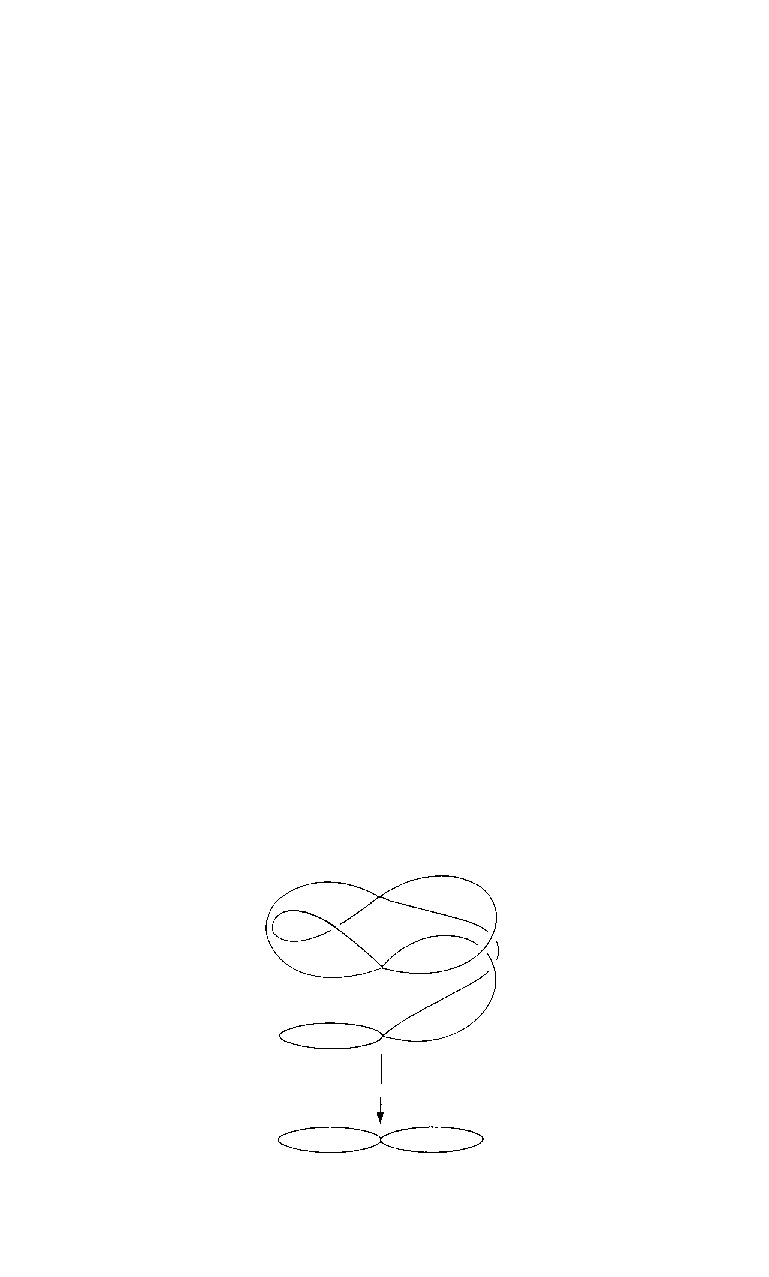
\includegraphics[width=0.4\textwidth]{Images/threefold_cover.pdf}
    \caption{This threefold cover of the figure eight space is not regular. Indeed, its group of automorphisms is trivial.}
    \label{fig:threefold-cover}
\end{figure}

\begin{rem}
    These ideas comprise the powerful \emph{Reidemeister-Schreier method} for finding presentations of subgroups $H\leq G$ given a presentation of $G$. Namely, one constructs a base space whose fundamental group is $G$, then finds a covering space corresponding to $H$ and computes its fundamental group.
\end{rem}

\begin{defn}
    Define the map $\Theta:N_G(G_{p_0})\to \mathrm{Aut}(\pi)$ by $\Theta(g)=a_g$ where $a_g$ is the unique deck transformation such that $a_g(p_0)=p_0\cdot g$.
\end{defn}
\begin{thm}[Classification of Deck Transformations {{\cite[Thm.~6.8]{Bredon}}}]\label{thm 6.8 Bredon}
    $\ker \Theta=G_{p_0}$, and consequently
    \[\mathrm{Aut}(\pi)\cong N_G(G_{p_0})\slash G_{p_0}.\]
\end{thm}
\begin{proof}
    First, 
    \[a_h(a_g(p_0))=a_h(p_0\cdot g)=a_h(p_0)\cdot g=(p_0\cdot h)\cdot g=p_0\cdot (hg)=a_{hg}(p_0).\]
    This proves that $\Theta$ is a homomorphism. Next note that if $a\in \mathrm{Aut}(\pi)$ then there is an $g\in N(G_{p_0})$ such that $a(p_0)=p_0\cdot g=a_g(p_0)$. Therefore $a=a_g$, which shows the surjectivity of $\Theta$.

    Finally we compute the kernel of $\Theta$. The result follows from the chain of equivalences
    \[a_g=\mathrm{id}_E \Leftrightarrow p_0\cdot g=p_0\Leftrightarrow g\in G_{p_0}.\]
\end{proof}
\begin{cor}
    If the covering map $E\overset{\pi}{\to} M$ is regular, then 
    \[\mathrm{Aut}(\pi)\cong G/G_{p_0}\]
\end{cor}
\begin{cor}
    If $\wt{M}\overset{\wt\pi}{\to} M$ is a universal covering map then
    \[\mathrm{Aut}(\wt\pi)\cong G=\pi_1(M,x_0).\]
\end{cor}



\subsection{Classification of covering spaces}

Our examination of connected covering spaces allows us to easily prove the following classification of connected covering spaces in terms of subgroups of the fundamental group of the base.

\begin{thm}[Classification of covering maps I]
    Let $M$ be path-connected and semilocally simply connected so that it has a universal covering space $\wt{M}$. Then the following \emph{Galois correspondence} holds:
\begin{enumerate}
	\item The isomorphism classes of connected pointed covering spaces of $M$ are in one-to-one correspondence with subgroups of $G=\pi_1(M, x_0)$. 
	\item The isomorphism classes of connected covering spaces of $M$ without basepoints are in one-to-one correspondence with the conjugacy classes of subgroups of $G=\pi_1(M, x_0)$.
    % sets $F$ (finite or countable) with an action of the group $\pi_1(M)$ (a group action on $F$ is an element of $\Hom(\pi_1(M),G)$, where $G$ is the full permutation group of the points of $F$).
\end{enumerate}
The correspondence is given by $E\leftrightarrow \pi_\ast(\pi_1(E,p_0))=G_{p_0}$ where $\pi$ is the covering map.
\end{thm}
\begin{proof}
    The second statement follows from the first combined with Corollary~\ref{cor 6.5 Bredon}. It remains to show that the map taking a covering map with a basepoint, $\pi:(E,p_0)\to (M,x_0)$, into the subgroup $\pi_\ast(\pi_1(E,p_0))$ of $\pi_1(M,x_0)$ is a bijection. It is an injection by the Lifting Theorem~\ref{Lifting Theorem}. 
    
    To see that it is a surjection, suppose that $H\subset \pi_1(M,x_0)=G$ is a subgroup. Since $\wt{M}$ is simply connected, Theorem~\ref{thm 6.8 Bredon} gives the isomorphism $\Theta:G\to \mathrm{Aut}(\pi)$, where $\Theta(g)=a_g$. Under this map, $H$ is mapped to a subgroup $A_H\leq \mathrm{Aut}(\pi)$. Put $E=\wt{M}/A_H$ which projects to $M$ canonically. Let $p_0$ be the image of the basepoint $\wt{p}_0\in\wt{M}$. We wish to identify $\pi_\ast(\pi_1(E,p_0))$. Let $\gamma$ be a loop in $X$ at $p_0$. Lifting this to $\wt{M}$ at $\wt{p}_0$ gives the same path as a lifting of the projection of $\gamma$ to a loop at $x_0$ in $M$. Thus the lifting ends at $a_g(\wt{p}_0)$, where $g\in\pi_1(M,x_0)$ is the homotopy class of the projection of $\gamma$ to $M$. But for $\gamma$ to be a loop in $E=\wt{M}/A_H$, we must have that $\wt{p}_0$ and $a_g(\wt{p}_0)$ are in the same orbit of $A_H$. This is true iff $a_g\in A_H$, and this holds iff $g\in H$. But $g$ is an arbitrary element of $\pi_\ast(\pi_1(E,p_0))$. Thus $H=\pi_\ast(\pi_1(E,p_0))$.
\end{proof}


Now we restate the classification theorem as it was described in Example~\ref{covering category thm}. We consider all, not only connected, coverings. 

Given an action of a group $G$ on a space $X$, the space $X$ decomposes into a disjoint union of orbits of $G$. Let us assume a discrete topology on $G$, in which case a continuous/smooth action is simply one for which the maps $\Phi_g:X\to X$ are continuous/smooth for all $g$. The set of all orbits is denoted by $X\slash G$ and, if imbued with the quotient topology descended from $X$, is called the \emph{orbit space}. Note that the canonical projection $p:X\to X\slash G$ that takes a point to its orbit is open because for an open $U\subset X$, $p^{-1}(p(U))=\bigcup_g (g\cdot U)$, which is a union of open sets.

Every covering map of $M$ gives rise to an action of $G=\pi_1(M,x_0)$ on the fiber $F=F_{x_0}$. Under this action $F$ decomposes into a disjoint union of orbits $F_j$, each of them associated with a conjugacy class of stabilizer subgroups $H_j<G$. This determines a functor from the category $\mathsf{Cov}_M$ of coverings of $M$ to the category $G\mathsf{-Set}$ of sets with a (left) action of $G=\pi_1(M,x_0)$. If $F$ is a $G$-set with a transitive action of $G$, then the stabilizers of any two of its points are conjugate subgroups of $G$. Choosing $p_0\in F$ and denoting $H=G_{p_0}$, we have that $F$ is isomorphic to the set of cosets $G\slash H$, also called a \emph{homogeneous set}. From such a $G$-set $F$ we can easily reconstruct a connected covering space $\pi$ by taking the universal covering space $\wt{M}$ and letting $\pi:\wt{M}\to \wt{M}\slash H$ be the orbit map of the action of $H$ on $\wt{M}$. If $F$ is not homogeneous, then it is a disjoint union of homogeneous sets (orbits), and the corresponding covering space is a disjoint union of the corresponding connected ones. This provides a functor in the opposite direction. It is easy to check that these two functors are each other's quasi-inverses. We thus have the second version of the theorem.

\begin{thm}[Classification of coverings II {{\cite[Thm.~3.3.2]{tomDieck}}}]\label{covering spaces category equivalence thm}
    If $M$ admits a universal covering space, then the category $\mathsf{Cov}_M$ is equivalent to the category $\pi_1(M)\mathsf{-Set}$. The corresponding functor returns the action of $\pi_1(M)$ on the fiber of the covering space and restricts morphisms to the fiber. Its quasi-inverse reconstructs a connected component of a covering space from each orbit of the $\pi_1(M)$-set as the quotient of the universal covering by the action of the stabilizer subgroup. Similarly, $\mathsf{Cov}_{M\bullet}$ is equivalent to $\pi_1(M)\mathsf{-Set}_\bullet$.
\end{thm}

\begin{rem}
    An action of a group $G$ on a set $X$ is really a homomorphism from $G$ into the group $\mathrm{Aut}(X)$ of automorphisms (bijective mappings, a.k.a.~permutations) of $X$. The element of $\Hom(\pi_1(M),\mathrm{Aut}(F))$ representing a given covering space is called the \emph{characteristic class}\index{Characteristic class} of this covering space. Therefore for a given discrete fiber $F$, all covering spaces of $M$ with fiber $F$ are completely classified by a characteristic class that is a contravariant functor from the category $\mathsf{Cov}_M(F)$ of all such covering spaces to the category of $\pi_1(M)$ actions on $F$.
\end{rem}

The next Corollary follows from the fact that the fundamental group $\pi_1$ is a homotopy invariant.
\begin{cor}
    The isomorphism classes of covering spaces of two base manifolds that are homotopy equivalent are in one-to-one correspondence. That is, the set of (isoclasses of) covering spaces is a homotopy invariant. 
\end{cor}


\begin{rem}
    Due to the path lifting property, we have a set-valued \emph{transport functor}\index{Transport functor} $T_\pi:\Pi(M)\to \mathsf{Set}$ on the fundamental groupoid that takes a path $\gamma$ in $M$, say connecting $x\in M$ to $y\in M$, and produces a map $T_\pi[\gamma]:F_x\to F_y$. Thus $T_\pi$ is an element of the category $[\Pi(M),\mathsf{Set}]$ consisting of functors from $\Pi(M)$ to $\mathsf{Set}$ and natural transformations between them. A morphism of covering spaces also induces a natural transformation between their transport functors (covariantly), therefore we have a functor $T:\mathsf{Cov}_M\to [\Pi(M),\mathsf{Set}]$. The classification theorem can be restated in yet another form: if $M$ is path-connected and semilocally simply connected, then $T$ is an equivalence of categories.
\end{rem}


Now we focus on regular coverings and to each such covering associate a functor that produces other (non-regular) coverings, providing another valuable version of the classification theorem. 

\begin{defn}[Properly discontinuous action]\index{properly discontinuous action}
    An action of a group $G$ on a space $X$ is properly discontinuous if each point $x\in X$ has a neighborhood $U$ such that $\exists\, g\cdot U\cap U\neq \varnothing \Leftrightarrow g=e$.
\end{defn}
\begin{rem}
    Any properly discontinuous action is free. Indeed, suppose $g\cdot x=x$ for some $g\in G$ and $x\in X$. Then the neighborhood $U$ of $x$ guaranteed to exist by definition of a properly discontinuous action necessarily satisfies $g\cdot U\cap U\neq\varnothing$, and therefore $g=e$. Hence the action is free.
\end{rem}

\begin{defn}[$G$-principal covering]
    A right $G$-principal covering is a covering map $\pi:E\to B$ with a properly discontinuous action of $G$ on $E$ such that $\pi(p\cdot g)=\pi(p)$ for all $(g,p)\in G\times E$ and such that the induced action on each fiber is transitive.
\end{defn}

\begin{example}
    The orbit map $E\to E\slash G$ of any properly discontinuous action is obviously a $G$-principal bundle. Conversely, every $G$-principal covering $\pi:E\to B$ induces a homeomorphism $\pi':E\slash G\cong B$ given by $p\cdot G\mapsto \pi(p)$. Indeed, since the action is transitive, the fiber $\pi^{-1}(x)$ coincides with the orbit $p\cdot G$ for any $p\in\pi^{-1}(x)$. Hence an inverse to $\pi'$ is given by $x\mapsto \pi^{-1}(x)=p\cdot G$. Its continuity follows from the fact that $\pi$ is a local homeomorphism.
\end{example}

We now examine the relationship between principal and regular coverings. 

\begin{prop}[{{\cite[Prop.~3.1.8]{tomDieck}}}]
    Let $\pi:E\to B$ be a covering map. Then:
    \begin{enumerate}[label=(\alph*)]
        \item If $E$ is connected, then the action of $\Aut(\pi)$ (an any of its subgroups) is properly discontinuous.
        \item Let $B$ be locally path connected and let $H$ be a subgroup of $\Aut(\pi)$. Then the map $\pi':E\slash H\to B$ induced by $\pi$ is a covering map.
    \end{enumerate}
\end{prop}
\begin{proof}
    (1) Let $p\in E$ and $g\in \Aut(\pi)$. Let $U$ be an evenly covered neighborhood of $\pi(p)$, and let $U_p$ be the sheet over $U$ containing $p$. For $q\in U_p\cap gU_p$ we have $\pi(q)=\pi(g^{-1}q)$, since $g^{-1}$ is an automorphism. Hence $q=g^{-1}q$, since both elements are contained in $U_p$. This shows $g^{-1}=e$, hence $U_p\cap gU_p=\varnothing$ for $g\neq e$, and we see that the action is properly discontinous.

    (2) Let $U\subset B$ be open, path connected, and evenly covered. Let $\pi^{-1}(U)=\bigcup_j U_j$ be the decomposition into sheets over $U$. An element $h\in H$ permutes the sheets, since they are the path components of $\pi^{-1}(U)$. The equivalence classes with respect to $H$ are therefore open in the quotient topology of $E\slash H$ and are mapped bijectively and continuously under $\pi'$. Since $\pi$ is open, so is $\pi'$. Hence $\pi'$ is trivial over $U$. Since $B$ is locally path connected, it has an open covering by such sets $U$.
\end{proof}
\begin{cor}
    A $G$-principal covering $\pi:E\to B$ induces a homeomorphism $E\slash G\cong B$.
\end{cor}

Thus the group $\mathrm{Aut}(\pi)$ of deck transformations of any covering space $E\overset{\pi}{\to}M$ acts properly discontinuously, and if $\pi$ is regular, this action is transitive on each fiber. Therefore 
\begin{center}
    a regular covering $\pi$ is an $\Aut(\pi)$-principal covering.
\end{center}

Now we ask the opposite question: what kind of coverings can properly discontinuous actions give rise to?

\begin{prop}
    If $G$ acts properly discontinuously on a path-connected and locally path-connected Hausdorff space $E$, then the \emph{orbit map} $\pi:E\to E\slash G$ is a regular covering map with deck transformation group $\mathrm{Aut}(\pi)=G$.
\end{prop}
\begin{proof}
    Let $U\subset X$ be a path-connected open set as in the definition of properly discontinuous actions and put $U^\ast =\pi(U)$, which is open as remarked above. Since $U\to U^\ast$ is continuous, $U^\ast$ is path-connected. Also, the sets $g\cdot U$ are the components of $\pi^{-1}(U^\ast)$. The maps $g\cdot U\to U^\ast$ are continuous, open, injective and surjective, and hence homeomorphisms. Thus $\pi$ is a covering map. Elements of $G$ are deck transformations and act transitively on the fiber. There are no other deck transformations by Lemma~\ref{lem 4.4 Bredon}.
\end{proof}
\begin{cor}
    If $X$ is simply connected and locally path-connected and $G$ acts properly discontinuously on $X$, then $\pi_1(X\slash G)\cong G$.
\end{cor}


Now let $\pi$ be a $G$-principal covering, so that $\pi$ induces a homeomorphism $E\slash G\cong B$, and by the above Proposition $\Aut(\pi)\cong G$. Therefore every principal covering is regular. We conclude that 
\begin{center}
    a $G$-principal covering $\pi$ is a regular covering with group of deck transformations $G$.
\end{center}


We now explain how, given a regular (or principal) covering, one can produce other coverings.

\begin{defn}[Associated covering]
    A right $G$-principal covering $\pi:E\to B$ gives rise to associated coverings. Let $F$ be a set with left $G$-action (a \emph{$G$-set}). Denote by $E\times_G F$ the quotient space $E\times F\slash \sim $ under the equivalence relation $(p,f)\sim(p\cdot g^{-1},g\cdot f)$ for $(p,f,g)\in E\times F\times G$. The continuous map $\pi_F:E\times_G F\to B$, $(p,f)\mapsto \pi(p)$ is a covering with fiber $F$.

    A $G$-equivariant map $\psi:F_1\to F_2$ induces a morphism of coverings
    \[\mathrm{id}_E\times_G\psi: \; E\times_G F_1\to E \times_G F_2,\; (p,f)\mapsto (p,\psi(f)).\]
\end{defn}

Thus for every right $G$-principal covering $\pi$ (over some base $B$) we have constructed the ``associated covering functor'' $A(\pi):G\mathsf{-Set}\to \mathsf{Cov}_B$ from the category of left $G$-sets (and equivariant maps) to the category of covering spaces of $B$. 

\begin{defn}[Universal $G$-principal covering]
    We call a $G$-principal covering $\pi$ \textit{universal} (among all $G$-principal coverings over all possible base spaces) if the functor $A(\pi)$ is an equivalence of categories.
\end{defn}

The classification theorem~\ref{covering spaces category equivalence thm} can now be restated as follows.
\begin{thm}[Classification of covering maps III]
     If a covering map $\pi:E\to B$ is universal (i.e.\ $E$ is simply connected), then it is also universal $\pi_1(B)$-principal (i.e.\ the functor $A(\pi)$ is an equivalence of categories).
\end{thm}

In this sense, universal coverings are ``classifying objects'' for all other coverings. Now it is natural to ask whether the converse holds, i.e.\ whether every universal $G$-principal covering is the universal covering of some space $B$ such that $\pi_1(B)\cong G$. For this it suffices to show that any universal $G$-principal covering must be simply connected.

\begin{prop}
    Let $B$ be a space which admits a universal covering. If a right $G$-principal covering  $\pi:E\to B$ is universal, then $E$ is simply connected, i.e.\ $\pi$ is a universal covering of $B$.
\end{prop}
\begin{proof}
    First consider the group $G$ acting on itself from the left as a $G$-set. It is clear from the definition that the associated bundle $A(\pi)(G)$ is isomorphic to $\pi$ itself. Now consider any other covering $\pi':E'\to B$. By assumption, $A(\pi):G\mathsf{-Set}\to \mathsf{Cov}_B$ is an equivalence of categories, thus there exists a left $G$-set $F$ such that the covering $A(\pi)(F)$ is isomorphic to $\pi'$. Now pick a point $p_0\in F$. The action $G\acts F$ induces a $G$-equivariant map $g\mapsto g\cdot p_0$. This is a morphism $f:G\to F$ in the category of $G$-sets. Sincce $A(\pi)$ is a functor, $A(\pi)(f)$ is a morphism from $A(\pi)(G)$ to $A(\pi)(F)$. Since $A(\pi)$ is an equivalence of categories, there is a natural transformation that turns this morphism into a morphism from $\pi$ to $\pi'$. Therefore $\pi$ is an initial object in the category $\mathsf{Cov}_B$, and hence isomorphic to the universal covering.
\end{proof}

We thus have the following abstract reformulation of the classification theorem, which will be a useful reference point for when we classify general fiber bundles.

\begin{thm}[Classification of covering maps IV {{\cite[Thm.~3.4.3]{tomDieck}}}]
    A covering map $\pi:E\to B$ is universal $G$-principal for some group $G$ iff it is a universal covering map of $B$ and $G\cong \pi_1(B)$.
\end{thm}
Note that for a fixed $G$ there are many non-isomorphic universal $G$-principal coverings: the universal covering of any space $B$ whose fundamental group is $G$ will work. 

\begin{rem}\label{rem: classifying space for discrete G}
    We will later learn to construct, for any discrete group $G$, a space $X_G$ whose fundamental group is isomorphic to $G$ and which admits a universal covering. Therefore for every group $G$ there exists a universal $G$-principal covering, although it is not unique. Once we learn about $CW$-complexes we will be able to define a special universal $G$-principal covering that is unique up to homotopy (namely the universal covering of the first Eilenberg-MacLane space $\rmK(G,1)$, see Section~\ref{sec: CW approx}). This fact will eventually have a natural extension to all groups and fiber bundles: for any group $G$ we will construct a so called classifying space $\rmB G$ and a principal $G$-bundle $\rmE G\to \rmB G$ such that $\rmE G$ is contractible. There will hold isomorphisms $\pi_{n+1}(\rmB G)\cong \pi{n}(G)$ for all $n\geq 0$. In the case of discrete $G$ the bundle $\rmE G\to \rmB G$ is obviously a covering space, and the aforementioned space $X_G$ provides a universal covering that is an ``approximation'' of this space, and for which only the first isomorphism $\pi_1(B)\cong \pi_0(G)\cong G$ holds.
\end{rem}

Since every covering space is a disjoint union of its connected components, let us separately address the classification of \emph{connected} covering spaces in terms of equivalence of certain categories. Let $\pi:E\to B$ be a universal right $G$-principal covering. A left $G$-set $A$ is a disjoint sum of its orbits. We thus have a corresponding decomposition of the total space $E\times_G F$ into the sum of $E\times_G C$, where $C$ runs over the orbits of $F$. An orbit is a transitive $G$-set and is isomorphic to a homogeneous set (set of cosets) $G\slash H$ of some subgroup $H<G$. The homeomorphism $E\times_G G\slash H\cong E\slash H$ shows that the summands $E\times_G C$ are path-connected. The action of $H$ on $E$ is properly discontinuous and therefore $E\to E\slash H$ is an $H$-principal covering. Also the induced map $\pi_H:E\slash H\to B$ is a covering.

The category of homogeneous $G$-sets and $G$-equivariant maps is called the \emph{orbit category} $\mathsf{Orb}(G)$. The sets $G\slash K$ and $G\slash L$ are isomorphic iff the subgroups $K$ and $L$ are conjugate in $G$. The stabilizers of points of $G\slash H$ are conjugate to $H$. The inclusion of the subcategory $\mathsf{Orb}(G)$ into the category of transitive $G$-sets is an equivalence.

Let $\wt{\pi}:\wt{E}\to B$ be a universal right $G$-principal covering with simply connected $E$. Then the functor $A(\wt{\pi})$ induces an equivalence of $\mathsf{Orb}(G)$ with the category of connected coverings of $B$. Each connected covering is thus isomorphic to a covering of the form $\pi_H:\wt{E}\slash H\to B$ for a subgroup $H<G$.

Let $\pi:E\to B$ be a connected covering. The subgroup $\pi_\ast(\pi_1(E,p_0))\subset \pi_1(B,x_0)$ is called the characteristic subgroup $C(\pi,p_0)$ of $\pi$ with respect to $p_0$. Different basepoints $p_0$ lead to conjugate characteristic subgroups, and conversely, every subgroup conjugate to $C(\pi,p_0)$ arises this way. We summarize these results in the final version of the classification theorem:

\begin{thm}[Classification V {{\cite[Thm.~3.4.4]{tomDieck}}}]
    If $M$ admits a universal covering space, then the category of connected coverings of $M$ is equivalent to the orbit category $\mathsf{Orb}(\pi_1(M,x_0))$. The isomorphism class of a connected covering $\pi:E\to M$ corresponds under this equivalence to the isomorphism class of $\pi_1(M,x_0)\slash C(\pi,p_0)$ for any $p\in\pi^{-1}(x_0)$. The isomorphism class of a connected covering is determined by the conjugacy class of its characteristic subgroup.
\end{thm}







\subsection{Examples of covering spaces}

\begin{example}[Covers of $\bbS^1$ and $\mathbb{C}^\ast$]
    The example that illustrates all the basic features of this theory is $M=\bbS^1$ (which we will represent by unit complex numbers). The universal cover is clearly $\wt{M}=\bbR $ with $\wt\pi(x)=\rme^{2\pi\rmi x}$. The deck transformations of $\wt M$ consist of integer shifts $x\mapsto x+n$, $n\in \bbZ$, therefore $\Aut(\wt M)=\bbZ$. And indeed, $\pi_1(\bbS^1)=\bbZ$. This universal cover can be interpreted as a slice of the Riemann surface of the complex logarithm $w=\ln z$, since the projection on this Riemann surface is exactly $\rme^w$. In fact, the entire Riemann surface (homeomorphic to $\mathbb{C}$) itself is the universal cover of $\mathbb{C}^\ast=\mathbb{C}\setminus\{0\}$. Since $\mathbb{C}^\ast$ and $\bbS^1$ are homotopy equivalent, their covering spaces are in one-to-one correspondence.

    Furthermore, all subgroups of $\bbZ$ have the form $k\cdot \bbZ$, $k\in\mathbb{N}$. The case $k=0$ gives rise to the simply-connected universal cover with $\pi_1(\wt M)=\{0\}$. Other values of $k$ give rise to total spaces that are homeomorphic to $\bbS^1$ but the covering map is $\pi_k(\rme^{\rmi t})=\rme^{\rmi kt}$. These are the $k$-sheeted covers that can also be interpreted as slices of the Riemann surfaces of the complex roots $z^{1/k}$, since the projections on them are exactly $z^k$.
\end{example}

\begin{example}[Universal covers of graphs]
    Let $M=\Gamma$ be a connected graph with $V$ vertices and $E$ edges, i.e.\ a topological space consisting of $E$ copies of the interval $[0,1]$ some of which are glued to each other at their ends. Such a graph always has a maximal tree, i.e.\ a subgraph of $\Gamma$ that is a tree and is not contained in any other sub-tree of $\Gamma$. One can show that a maximal tree must contain all vertices of $\Gamma$. Since every tree is a contractible topological space, by retracting a maximal tree of $\Gamma$ into one point we identify all vertices of $\Gamma$ into one point. This shows that $\Gamma$ is homotopy equivalent to the wedge sum of some number of circles, each corresponding to a cycle in the graph. Namely, the number $l$ of cycles in $\Gamma$ equals the number of edges in $\Gamma$ minus the number of edges in a maximal tree of $\Gamma$. This is also equal to $1-\chi(\Gamma)$, where $\chi(\Gamma)=V-E$ is the Euler characteristic. Then by Proposition~\ref{prop computing pi1}, $\pi_1(\Gamma)$  is a free group with $l$ generators. Finally, from the above results it is easy to see that $\wt{\Gamma}$ is the \href{https://en.wikipedia.org/wiki/Cayley_graph}{Cayley graph} of this free group, i.e.\ the graph whose vertices are all the elements of the group, and the edges incident to a vertex correspond to the generators of the group and their inverses. The vertex on the other end of an edge is the result of the multiplication of the current vertex by the edge's generator (say, from the right). In the case of a free group with $l$ generators, this is a regular tree whose root represents the identity element and each vertex has valency/degree (number of incident edges) equal to $l$. See Fig.~\ref{Fig. Cayley} for an example of a Cayley graph.
\end{example}
\begin{figure}
    \centering
        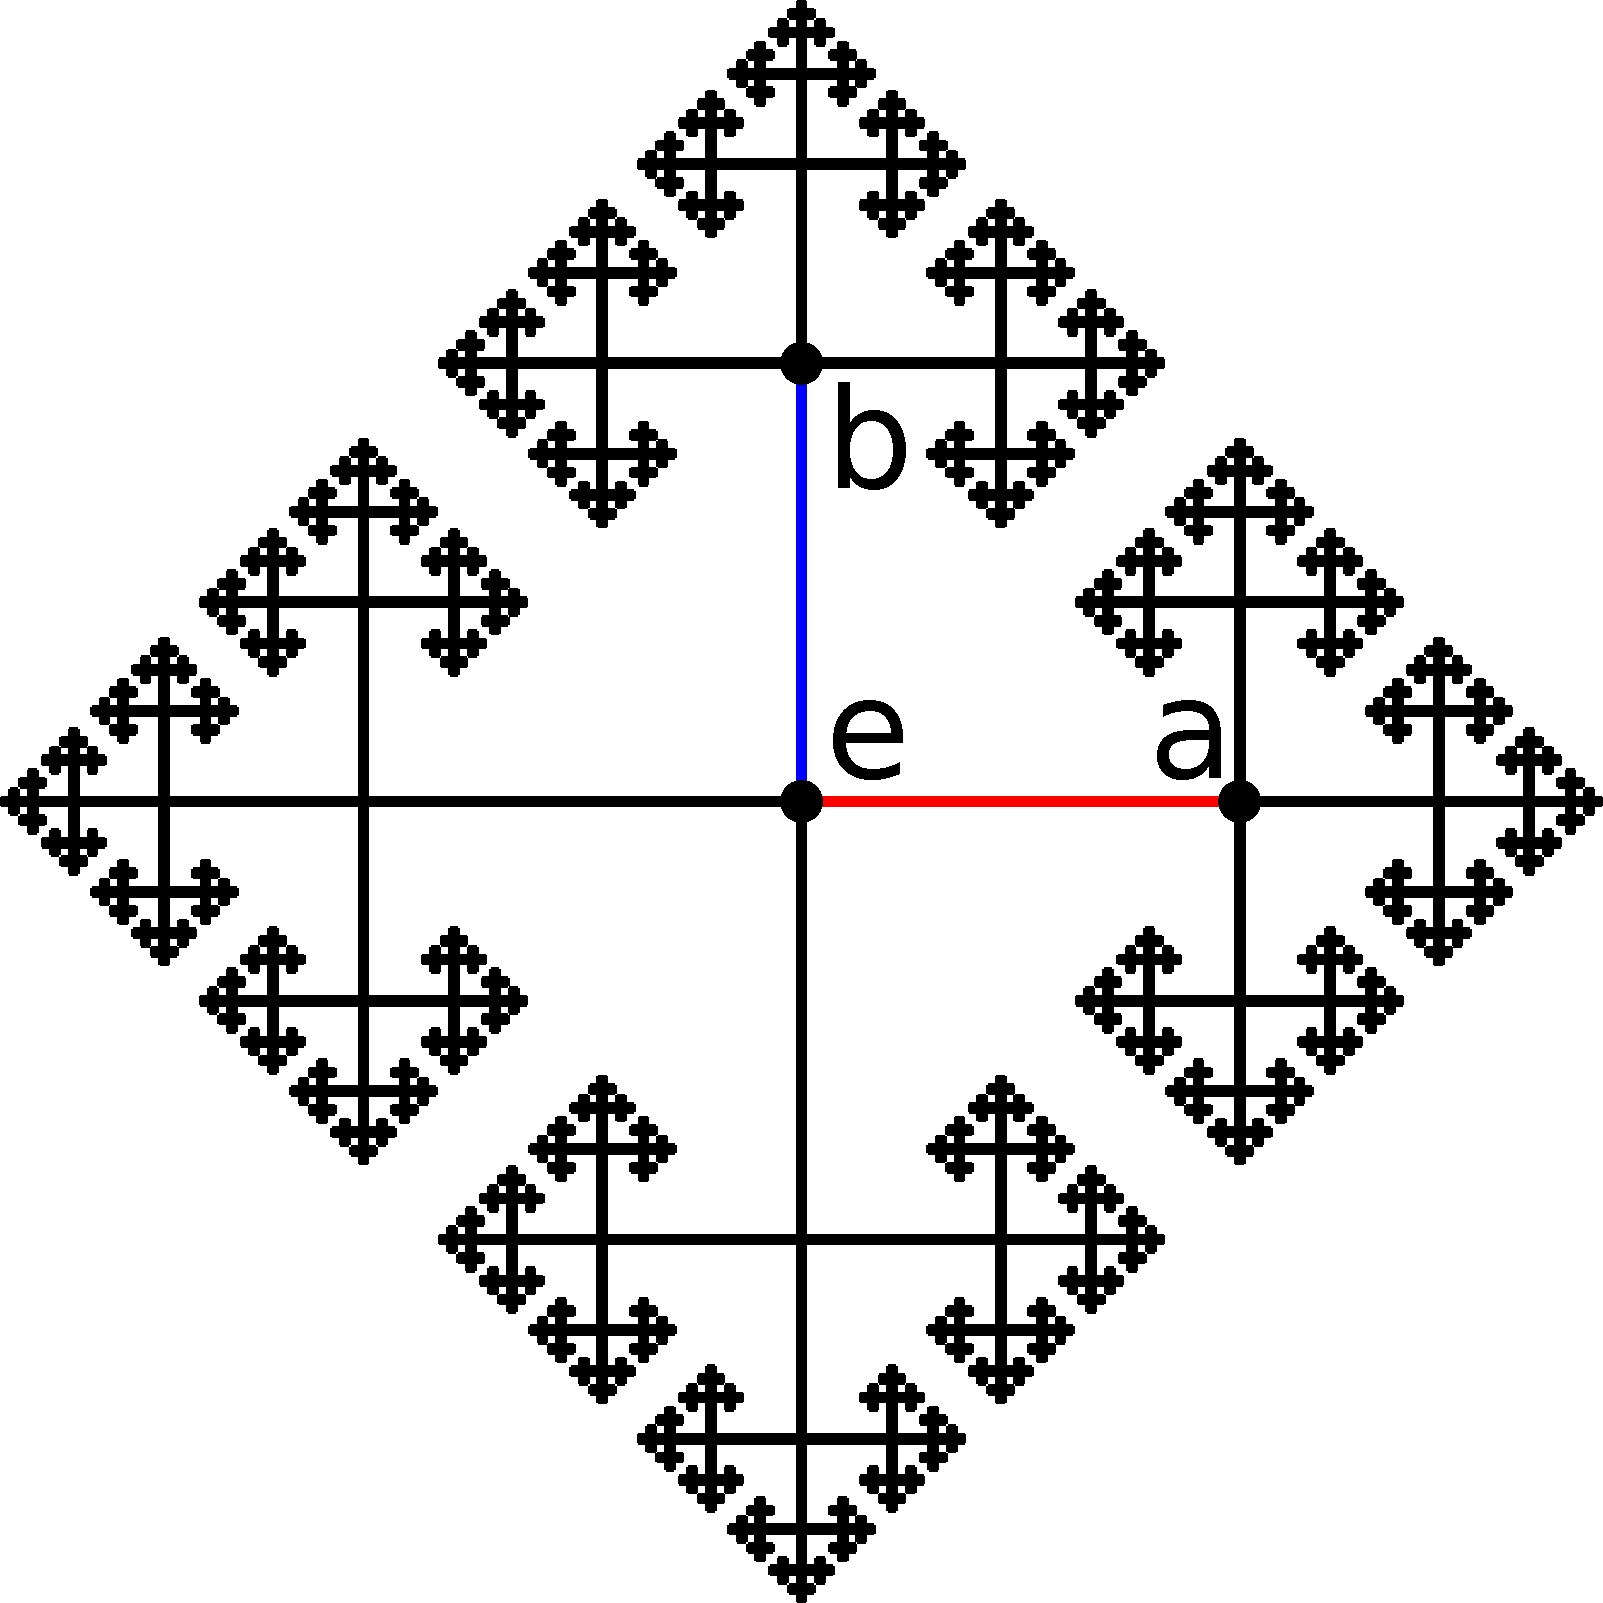
\includegraphics[scale=0.15]{Images/Cayley.pdf}
    \caption{This graph is the universal cover of the figure eight, which is $\Gamma=\bbS^1 \vee \bbS^1$. It is also the Cayley graph of the fundamental group of $\Gamma$, i.e.\ the free group with two generators $a$ and $b$, $\pi_1(\Gamma)=F(\{a,b\})\cong\bbZ\ast\bbZ$. \label{Fig. Cayley}}
\end{figure}

We can now use the theory of covering spaces to prove a very important basic theorem about free groups. 
\begin{thm}[Nielsen-Schreier]\index{Theorem!Nielsen-Schreier}\label{thm Nielsen-Schreier}
    Any subgroup of a free group is free.
\end{thm}
\begin{proof}
    Let $G$ be a free group. As we've seen, it can be realized as the fundamental group of a \emph{bouquet} $M=\bigvee \bbS^1$ of as many circles as there are generators in $G$. Given a subgroup $H\leq G$, there must exist a covering space $E\overset{\pi}{\to}M$ such that $H=\pi_\ast(\pi_1(E,p_0))$ and $\pi_\ast:\pi_1(E,p_0)\to H\subset \pi_1(M,x_0)$ is an isomorphism. However, any covering space of a graph is a graph (indeed,each edge incident with a vertex in the base can be uniquely lifted to the total space, these liftings are homeomorphisms, and doing so for all vertices gives the total space a structure of a graph). In particular, any covering space of a bouquet of circles is a bouquet of circles. This implies that the fundamental group of $E$ is free, and therefore $H$ is free.
\end{proof}
\begin{cor}
    If a subgroup of a free group of finite rank has finite index, then it is also of finite rank.
\end{cor}
\begin{proof}
    Indeed, if $H\leq G$ has finite index, it can be realized as the fundamental group of a finite covering graph of a finite bouquet of circles. But any such graph has a finitely generated fundamental group.
\end{proof}
\begin{thm}[Schreier formula]
    If $G$ is a free group of finite rank $r_G$ and $H \leq G$ is a subgroup of finite index $n$, then $H$ is free of rank $r_H=n(r_G-1)+1$.
\end{thm}
\begin{proof}
    Let $G=F(x_1,\ldots,x_{r_G})$. This follows from examining the covering graph constructed in Theorem~\ref{thm Nielsen-Schreier}. It has one vertex for each right coset $Hg$ and exactly $2r_G$ edges at each vertex ($r_G$ going in and $r_G$ going out) with the outgoing edge going from $Hg$ to $Hgx_i=(Hg)\cdot x_i$ labeled by the generator $x_i$. Therefore this graph has $V=n$ vertices and $E=nr_G$ edges. The fundamental group of this graph $\wt\Gamma$ is isomorphic to $H$ and is generated by $1-\chi(\wt\Gamma)=1-V+E=n(r_G-1)+1$ loops.
\end{proof}
\begin{cor}
    Let $\Gamma$ be a covering graph of $\bigvee_{i=1}^r \bbS^1$ (with $r>1)$ that corresponds to a subgroup generated by $r'>1$ generators. If $n=(r'-1)/(r-1)$ is a positive integer then $\Gamma$ has $n$ sheets, otherwise $\Gamma$ has infinitely many sheets.
\end{cor}
\begin{cor}
    The free group of two generators, $F(a,b)$, contains free subgroups of any integer rank $r_H$. 
\end{cor}
\begin{proof}
    The set of all words whose degree (the sum of the powers of all generators in it) equals $r_H$ is one such subgroup.

    Alternatively, we can simply notice that the space $\bbS^1\vee \bbS^1$ has covering spaces that are homeomorphic to $\bigvee_{i=1}^r \bbS^1$ for any $r$.
\end{proof}

\begin{example}[Covering spaces of $\bbS^1\vee \bbS^1$]
    Consider the ``figure eight'' space $M=\bbS^1\vee \bbS^1$. Its covering spaces are in one-to-one correspondence with conjugacy classes of subgroups of the free group $F(a,b)$ of two generators (one for each circle in $M$). By Theorem~\ref{thm Nielsen-Schreier}, any subgroup of a free group is free, so each covering space of $M$ is uniquely determined by a subset of $F(a,b)$ that contains no relations (e.g.\ the set $\{a^2,b^2,a^2b^2\}$ is redundant and should be replaced with $\{a^2,b^2\}$). The elements of this subset generate the image of $\pi_1(E,p_0)$ under the monomorphism $\pi_\ast$.

    Some examples of these covering spaces are given in Figures~\ref{fig:sixfold covering} and \ref{fig:coverings of 8}. The covering in Figure~\ref{fig:threefold-cover} is another one. It is instructive to observe which of the coverings in Figure~\ref{fig:coverings of 8} are regular, and how the subgroups corresponding to them are normal. It is similarly instructive to verify the Lifting Theorem~\ref{Lifting Theorem}: two different covering spaces of $M$ are covering spaces of each other (say with basepoints) only if the generators of the stabilizer of one of them can be expressed in terms of the generators of the other. For example, (11) is a covering space of (1) because  $b^nab^{-n}=(b^2)^{n/2}a(b^{-2})^{n/2}$ if $n$ is even and $b^nab^{-n}=(b^2)^{(n-1)/2}bab^{-1}(b^{-2})^{(n-1)/2}$ otherwise.

    (1) and (2), up to swapping $a$ and $b$, are all of the existing connected double covers (so there are three in total). (3) and (4) are the same covering space but with different basepoints, and one can see how the corresponding subgroups are conjugates of each other by an element that connects those two points, for example $b$.
\end{example}

\begin{figure}
    \centering
    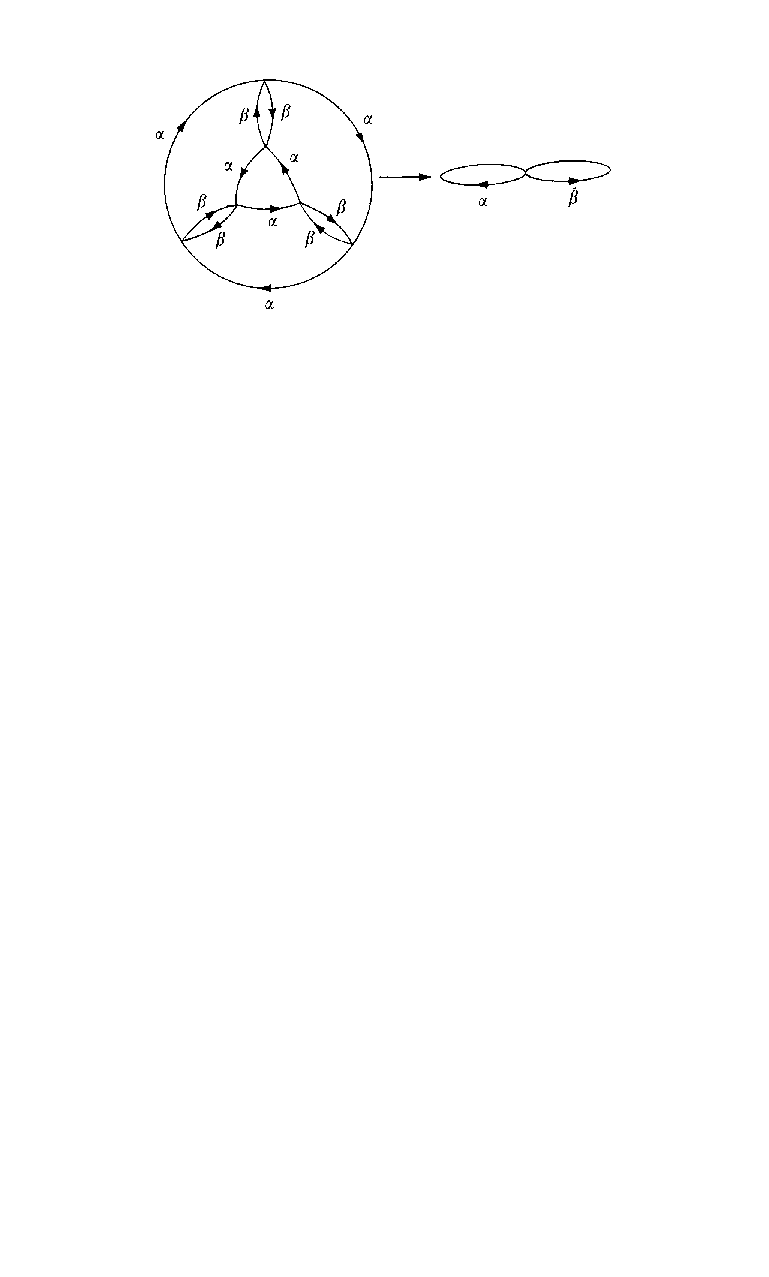
\includegraphics[width=0.6\textwidth]{Images/sixfold.pdf}
    \caption{A sixfold regular covering space of the figure eight. The fundamental group $\pi_1(E,p_0)$ is clearly generated by six loops. This makes it easy to guess that the stabilizer of any vertex is the normal subgroup of the free group $F(\alpha,\beta)$ generated by the six elements $\alpha^3,\beta^2,\left(\alpha\beta^{-1}\right)^2, \left(\alpha^{-1}\beta\right)^2, \alpha\beta^2\alpha^{-1}, \alpha^{-1}\beta^2\alpha$. To find the group of deck transformations, we factor the free group by this normal subgroup, which is equivalent to adding these six generators as relations. It is easy to check that these relations define the permutation group $S_3=\langle a,b\mid a^2,b^2,ababab\rangle$. If we reversed the arrows on the inner triangle of $\alpha$'s, we'd get $\bbZ_2\times \bbZ_3$ instead. From \cite[Fig.~III-7]{Bredon}.}
    \label{fig:sixfold covering}
\end{figure}

\begin{figure}
    \centering
    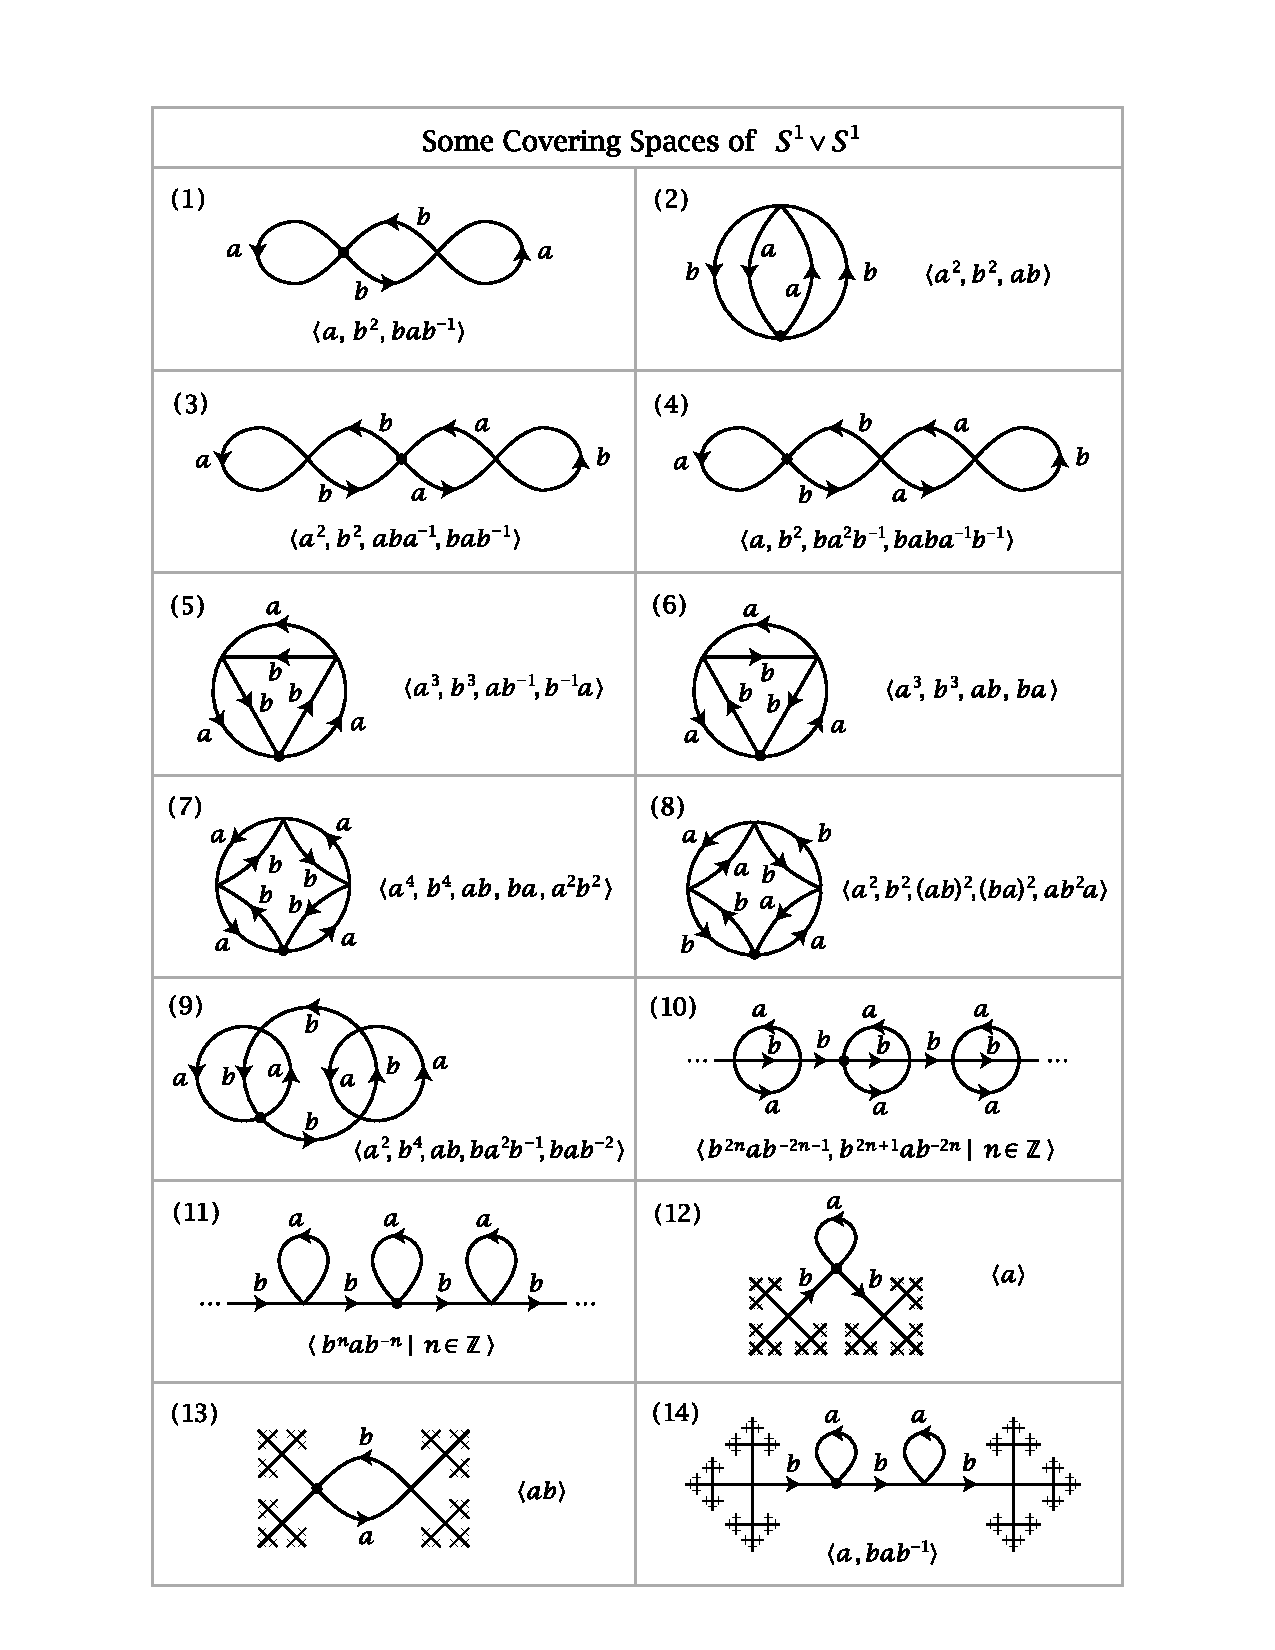
\includegraphics[width=0.67\textwidth]{Images/coverings_8.pdf}
    \caption{Examples of covering spaces of the figure eight space. Each one is a graph with a marked basepoint $p_0$ such that the neighborhood of each vertex locally looks the same as in the base space: two incoming edges (labeled $a,b$) and two outgoing (also labeled $a,b$). The label of an edge indicates which generator of $\pi_1(M)$ it is projected onto by $\pi$. Next to the space is the list of the generators of the local fundamental group $\pi_1(E,p_0)$ expressed in terms of $a,b$, which means that, viewed as part of $\pi_1(M)$, they generate the stabilizer $G_{p_0}=\pi_\ast(\pi_1(E,p_0))$. The number of sheets matches the index of this subgroup. Two vertices are related by a deck transformation iff their stabilizers coincide, otherwise the stabilizers are merely conjugate. For regular coverings (1,2,5,6,7,8,9,11), all stabilizers coincide and therefore are normal. From \cite[p.~58]{Hatcher}.}
    \label{fig:coverings of 8}
\end{figure}


\begin{xca}
    Show that the covering space of the figure eight space $M=\bbS^1\vee \bbS^1$ that corresponds to the normal subgroup generated by $a^2$, $b^2$, and $(ab)^4$ (where $a,b$ are the two generators of the free group $\pi_1(M)$) is regular, and describe what it looks like. \emph{Hint:} this subgroup has index 8, so it's an eight-fold covering.
\end{xca}

\begin{xca}
    Describe the covering space of the figure eight space that corresponds to the commutator subgroup of the free group of two generators. \emph{Hint:} $F(a,b)\slash [F(a,b),F(a,b)]=\bbZ^2$, so this covering space has a $\bbZ^2$-symmetry.
\end{xca}
\begin{xca}
    Identify in $\bbS^1$ the open upper and the open lower semicircle to a point. The resulting space $X$ has four points. Show $\pi_1(X)\cong \bbZ$. Does $X$ have a universal covering?
\end{xca}
\begin{xca}
    Show that the universal cover of $M_1\times M_2$ is $\wt M_1\times \wt M_2$.
\end{xca}
\begin{xca}[{{\cite[Exercise~B.7]{Hatcher}}}]
    If $G$ is a finitely generated free group and $N$ is a nontrivial normal subgroup of infinite index, show, using covering spaces, that $N$ is not finitely generated.
\end{xca}

\begin{example}
    $\widetilde{\bbT^n}=\bbR^n$, $\widetilde{\text{SO}_3}=\text{SU}_2=\bbS^3$, $\widetilde{\text{SO}}_{n>2}=\text{Spin}_n$, $\widetilde{\text{U}_n}=\text{SU}_n\times \bbR $.
\end{example}






\newpage
\section{Homotopy Theory}


\subsection{Homotopy groups}

\begin{defn}[Homotopy groups]\index{Homotopy groups}
Pick the base points $\bullet\in \bbS^n$ and $x_0\in X$. The set of homotopy classes of maps $\gamma:\bbS^n\to X$ such that $\gamma(\bullet)=x_0$ forms the $n$-th homotopy group $\pi_n(X,x_0)=[\bbS^n;X]_\bullet$. For two such maps, define their product by first mapping $\bbS^n$ onto the wedge sum $\bbS^n\lor \bbS^n$ via contracting an arbitrarily chosen equator (which is homeomorphic to $\bbS^{n-1}$) into one point, then apply $\gamma_1$ and $\gamma_2$ to the two hemispheres respectively, making the equator point the base point for them.

For $n=0$, $\pi_0(X)$ is defined as the set of path-connected components of $X$ (which is also the set of homotopy classes of pointed maps $\bbS^0\to X$) but does not have a natural group structure.
\end{defn}

\begin{xca}
\begin{enumerate}
    \item The above definition is consistent and the resulting homotopy classes don't in fact depend on the choice of an equator. In fact, in natural terms, this group operation is exactly the coproduct on the category of pointed spaces, given by the wedge sum $\gamma_1\lor\gamma_2:\bbS^n\lor \bbS^n\to X$ (a.k.a. \emph{concatenation}).
    \item All homotopy groups for different $x_0$ are isomorphic.
\end{enumerate}
\end{xca}


\begin{prop}[Functoriality of $\pi_n$]
    Any pointed continuous map $f:X\to Y$ induces a homomorphism of the homotopy groups $f_\ast:\pi_n(X,x_0)\to \pi_n(Y,y_0)$, and $(g\circ f)_\ast=g_\ast\circ f_\ast$. In other words, we have a \emph{functor} $\pi_n:\mathsf{Top}_\bullet\to \mathsf{Gr}$.
\end{prop}

\begin{thm}
Homotopy groups $\pi_n$, $n\geq 1$, are homotopy invariants, i.e.\ if $X\simeq Y$ are two homotopy equivalent path connected spaces, then $\pi_n(X,x_0)\cong\pi_n(Y,y_0)$.
\end{thm}
\begin{proof}
Exercise. Also see \cite{Hatcher}.
\end{proof}
\begin{cor}
    $\pi_n$ descends to a functor $\pi_n:\mathsf{hTop}_\bullet\to \mathsf{Gr}$ on the category $\mathsf{hTop}_\bullet$, in which the morphisms are the homotopy classes of pointed continuous maps modulo homotopy relative to the base point. In particular, homotopy equivalent spaces have isomorphic homotopy groups.
\end{cor}

\begin{thm}
For $n\geq 2$, all groups $\pi_n(X,x_0)$ are abelian.
\end{thm}
\begin{proof}
Follows from Proposition \ref{suspension maps prop} and the fact that $\bbS^n=\Sigma\Sigma \bbS^{n-2}$ for $n\geq 2$. We have $[\bbS^n,Y]=[\Sigma\Sigma \bbS^{n-2},Y]=[\Sigma \bbS^{n-2}, \Omega Y]$, which is abelian.
\end{proof}

Another very important connection between homotopy groups and suspension will be discussed when we prove Freudenthal's Suspension Theorem \ref{thm 6.4.7 tomDieck freudenthal}.

\begin{comment}
\PRLsep
\begin{center}
  {\red Lecture 4 on 30 Nov 2018 ended here}
\end{center}
\end{comment}



\subsection{Exact sequence of homotopy groups}

\begin{defn}[Topological triple]
    A triple $(X,A,B)$ is a topological space $X$ with a pair of subspaces $A\subset B\subset X$. When $B=\bullet$ is a point, the triple is also called a pointed pair.
\end{defn}

\begin{defn}[Relative homotopy groups]\index{Relative homotopy groups}\index{Homotopy groups!relative}
        For a pointed pair $(X,A,\bullet)$ and $n\geq 1$ the relative homotopy group $\pi_n(X,A,\bullet)$ is the set of homotopy classes of triples $\pi_n(X,A,\bullet)=[(\bbD^n,\bbS^{n-1},\bullet);(X,A,\bullet)],$
        where $\bbD^n$ is the $n$-disk, $\bbS^{n-1}$ is its boundary, and the homotopies are through pointed maps that take $\bbS^{n-1}$ into $A$. Note that this is \emph{not} the same as homotopies relative to $\bbS^{n-1}$.
\end{defn}
These are groups with the same multiplication operation and they are still abelian for $n\geq 3$ because $[(\Sigma X,\Sigma A);(Y,B)]=[( X, A);(\Omega Y,\Omega B)]$.
\begin{prop}[Compression criterion]\label{prop: compression criterion}
    A map $f:(\bbD^n,\bbS^{n-1},\bullet)\to (X,A,\bullet)$ represents the identity in $\pi_n(X,A,\bullet)$ iff it is homotopic $\rel \partial \bbD^n\cong \bbS^{n-1}$ to a map whose image is contained in $A$.
\end{prop}
\begin{proof}
    For necessity, a map whose image is contained in $A$ can be composed with a deformation retraction of $\bbD^n$ onto the basepoint to give a homotopy to a trivial map. Conversely, if $[f]=e$ via a homotopy $H:\bbD^n\times I\to X$, then by restricting $H$ to a family of $n$-disks in $\bbD^n\times I$ starting with $\bbD^n\times \{0\}$ and ending with the disk $\bbD^n\times\{1\}\cup \bbS^{n-1}\times I$, all the disks in the family having the same boundary, then we get a homotopy from $f$ to a map onto $A$, stationary on $\bbS^{n-1}$. This is a homotopy relative to $A$.
\end{proof}

Any map $f:(X,A,x_0)\to (Y,B,y_0)$ induces maps $f_\ast :\pi_n(X,A,x_0)\to \pi_n(Y,B,x_0)$ which are homomorphisms for $n\geq 2$ and have properties analogous to those in regular homotopy: $(f\circ g)_\ast=f_\ast\circ g_\ast$, $\mathrm{id}_\ast=\mathrm{id}$, and $f_\ast=g_\ast$ if $f\sim g$ through maps of pointed pairs $(X,A,x_0)\to(Y,B,y_0)$.

In particular, the inclusions $i:(A,x_0)\hookrightarrow(X,x_0)$ and $j:(X,x_0,x_0)\hookrightarrow (X,A,x_0)$ induce such homomorphisms. Moreover, there is a third special homomorphisms that connects homotopy groups in adjacent degrees.

\begin{defn}[Boundary operator for homotopy]
    The inclusion of the boundary $\bbS^{n-1}\hookrightarrow \bbD^n$ induces restrictions of maps $f:(\bbD^n,\bbS^{n-1},s_0)\to (X,A,x_0)$ to the boundary, i.e.\ $\partial f=\restr{f}{\partial \bbD^n}$. For $n\geq 2$ this operator defines a homomorphism of relative homotopy groups.
\end{defn}

\begin{defn}[Exact sequence]
    Let $\calC$ be a category in which the notions of kernels and images of morphisms are well-defined. For now we assume that it is a concrete category, so kernels and images are understood as subsets of the domain and codomain, respectively. Next let there be a (finite or infinite) sequence of morphisms
    \[\cdots\to X\overset{f}{\to } Y\overset{g}{\to} Z\to \cdots \]
    We say that this sequence is exact at $Y$ if $\im f=\ker g$.
\end{defn}
\begin{example}
    In the category of pointed sets (or topological spaces etc.), kernels can be defined as the pre-images of the basepoint. Exactness then amounts to $\im f=g^{-1}(*)$.

    Usually we will be concerned with the case $\calC=\mathsf{Gr}$.
\end{example}
\begin{defn}[Short exact sequence]
    A short exact sequence is a sequence of the form
    \[0\to X\overset{f}{\to } Y\overset{g}{\to} Z\to 0,\]
    where $0$ is a zero object in $\calC$.

    The exactness at $X$ is equivalent to $f$ being a monomorphism. Exactness at $Z$ is equivalent to $g$ being an epimorphism. The exactness at $Y$ essentially says that $Z\cong Y\slash \im f=Y\slash \ker g\cong Y\slash X$. In the category of groups this is just the first isomorphism theorem.
\end{defn}

\begin{example}
    If the short exact sequence is even shorter, e.g.
    \[0\to X\overset{f}{\to } Y\to 0,\]
    then its exactness is equivalent to $f$ being an isomorphism.
\end{example}

\begin{thm}[Long exact sequence of homotopy groups]\index{Long exact sequence!of homotopy groups}\label{thm long exact seq of homotopy}
    The sequence of homomorphisms
    \[\cdots \to \pi_n(A,x_0)\overset{i_\ast}{\to}\pi_n(X,x_0)\overset{j_\ast}{\to}\pi_n(X,A,x_0)\overset{\partial}{\to}\pi_{n-1}(A,x_0)\to \cdots \to \pi_0(X,x_0)\]
    is \emph{exact}. Near the end of the sequence, where the group structure is not defined, the ``kernel'' is the path-connected component of $x_0$.
\end{thm}
\begin{proof}
    In fact we will prove the long exact sequence of a pointed triple $(X,A,B,x_0)$ with $x_0\in B\subset A\subset X$:
    \begin{multline}
        \cdots \to \pi_n(A,B,x_0)\overset{i_\ast}{\to}\pi_n(X,B,x_0)\overset{j_\ast}{\to}\pi_n(X,A,x_0)\overset{\partial}{\to}\pi_{n-1}(A,B,x_0)\to \cdots \\ \to \pi_1(X,A,x_0).
    \end{multline}
    The boundary operator for triples is defined as the composition $\partial:\pi_n(X,A)\overset{\partial}{\to} \pi_{n-1}(A)\overset{i_\ast}{\to} \pi_{n-1}(A,B)$ where $i:B\hookrightarrow A$ is the inclusion map. When $B=\{x_0\}$ this reduces to the exact sequence of the pointed pair $(X,A,x_0)$, though the latter sequence continues for two more steps to $\pi_0(X,x_0)$.

    \emph{Exactness at} $\pi_n(X,B,x_0)$: First note that the composition $j_\ast\circ i_\ast$ is trivial since every map $(\bbD^n,\bbS^{n-1},s_0)\to (A,B,x_0)$ represents zero in $\pi_n(X,A,x_0)$ by the compression criterion. To see that $\ker j_\ast \subset \im i_\ast$, let $f:(\bbD^n,\bbS^{n-1},s_0)\to (X,B,x_0)$ represent the trivial element in $\pi_n(X,A,x_0)$. Then by the compression criterion again, $f$ is homotopic $\rel \bbS^{n-1}$ to a map with image in $A$, hence $[f]\in \pi_n(X,B,x_0)$ is in the image of $i_\ast$.

    \emph{Exactness at} $\pi_n(X,A,x_0)$: The composition $\partial\circ j_\ast$ is zero since the restriction of a map $(\bbD^n,\bbS^{n-1},s_0)\to (X,B,x_0)$ to $\bbS^{n-1}$ has image lying in $B$, and hence represents the trivial class in $\pi_{n-1}(A,B,x_0)$. Conversely, suppose the restriction of $f:(\bbD^n,\bbS^{n-1},s_0)\to (X,A,x_0)$ to $\bbS^{n-1}$ represents the trivial element $\pi_{n-1}(A,B,x_0)$. Then $\restr{f}{\bbS^{n-1}}$ is homotopic to a map with image in $B$ via a pointed homotopy $H:\bbS^{n-1}\times I \to A$. We can tack $H$ onto $f$ to get a new map $(\bbD^n,\bbS^{n-1},s_0)\to (X,B,x_0)$ which, as a map $(\bbD^n,\bbS^{n-1},s_0)\to (X,A,x_0)$, is homotopic to $f$ by the homotopy that tacks on increasingly longer initial segments of $H$. So $[f]\in \im j_\ast$.

    \emph{Exactness at} $\pi_n(A,B,x_0)$: The composition $i_\ast \circ \partial$ is trivial since the restriction of a map $f:(\bbD^{n+1},\bbS^n,s_0)\to (X,A,x_0)$ to $\bbS^n$ is homotopic $\rel s_0$ to a constant map via $f$ itself (via a contraction of $\bbS^n$ onto $s_0$ inside $\bbD^n$). The converse is easy if $B$ is a point, since the nullhomotopy $f_t:(\bbD^n,\bbS^{n-1})\to (X,x_0)$ of $f_0:(\bbD^n,\bbS^{n-1})\to (A,x_0)$ gives a map $F:(\bbD^{n+1},\bbS^n,s_0)\to (X,A,x_0)$ with $\partial([F])=[f_0]$. Thus the proof is finished in this case. 
    
    For a general $B$, let $f:(\bbD^{n},\bbS^{n-1},s_0)\to (A,B,x_0)$ be in the kernel of $i_\ast$ and let $F:\bbD^n\times I\to X$ be a corresponding nullhomotopy of $f$ through maps $(\bbD^n,\bbS^{n-1},s_0)\to (X,B,x_0)$. It is then clear that $F$ can be viewed as a map $\bbD^{n+1}\to X$ which restricts to $f$ on $\bbD^n\times \{0\}$, and maps the rest of the boundary into $B\subset A$, which makes $f$ the boundary of some map $(\bbD^{n+1},\bbS^n,s_0)\to (X,A,x_0)$.
\end{proof}



\subsection{\texorpdfstring{$CW$}{CW}-complexes}

\begin{defn}[$CW$-complex]\index{$CW$-complex}\index{Cell complex}
    A cellular structure on a set $X$ is a family $\mathcal{F}$ of \textit{characteristic mappings} $f_\alpha^n:\bbD^n\to X$, where $n=0,1,2,\ldots$ and $\alpha\in A_n$ (some indexing sets), such that the following conditions hold. Let $X^{(n)}$ denote the union of images of mappings $f_\alpha^k, k\leq n$. Also $X^{(-1)}=\varnothing$.
    \begin{enumerate}
        \item For every $n$, $\bigsqcup_\alpha f_\alpha^n$ maps $\bigsqcup_\alpha \Int \bbD^n$ \emph{injectively} to $X\setminus X^{(n-1)}$. Here, we put $\Int \bbD^0=\bbD^0$.
        \item Every $f_\alpha^n$ maps $\partial \bbD^n$ to $X^{(n-1)}$.
        \item $X=\bigcup_n X^{(n)}$.
    \end{enumerate}
    
    A $CW$-complex is a Hausdorff topological space with a $CW$-structure such that the topology coincides with the final topology defined by $\mathcal{F}$, also called the \emph{weak topology}\index{Weak topology}: $A\subset X$ is open iff $A\cap X^{(n)}$ is open in $X^{(n)}$ for each $n$.

    The restrictions $\partial f_\alpha^n=\restr{f_\alpha^n}{\partial \bbD^n}$ are called the \textit{attaching maps}. The subsets $X^{(n)}\subset X$ are called the $n$-skeleta of $\mathcal{F}$. The images $f_\alpha^n(\bbD^n)$ are referred to as the \textit{closed cells} and $f_\alpha^n(\Int  \bbD^n)$ as \textit{open cells} (even though these are actually closed or open only as subspaces of $X^{(n)}$!). A $CW$-complex $(X,\mathcal{F})$ is said to be pointed if $X$ is pointed and the basepoint is a $0$-cell. A subcomplex is a subspace $X'\subset X$ endowed with the relative topology, together with a subfamily $\mathcal{F}'\subset\mathcal{F}$ such that $(X',\mathcal{F}')$ is a $CW$-complex. The highest dimension of a cell in a complex is called its dimension. A $CW$-complex is called finite if it is finite-dimensional and has a finite number of cells.
\end{defn}

We will typically work with finite $CW$-complexes, but infinite-dimensional ones will be useful as well.

\begin{rem}
The acronym $CW$ refers to the following properties.
\begin{enumerate}
    \item Closure-finiteness: every closed cell meets only finitely many open cells, which we will prove in Proposition~\ref{prop 8.1 Bredon}.
    \item Weak topology: $X$ carries the final topology defined by the family $\mathcal{F}$.
\end{enumerate}
A  more general concept of cellular complexes drops these requirements. Note that, due to the inductive definition of $CW$-complexes as a collection of attaching maps, we get (C) automatically.
\end{rem}

% The following Proposition shows that the weak topology induced by any \emph{finite} $CW$-structure consisting of continuous characteristic maps  on a Hausdorff space coincides with the original topology.

% \begin{prop}[{{\cite[Prop.~3.1.9]{RS2}}}]\label{prop 3.1.9 RS2}
%     Let $X$ be a Hausdorff space and let $\mathcal{F}$ be a finite $CW$-structure on $X$. For $\mathcal{F}$ to make $X$ into a $CW$-complex it suffices that every $f_\alpha^n\in\mathcal{F}$ be continuous.
% \end{prop}
% \begin{proof}
%     We show that a subset $A \subset X$ is closed iff $(f_\alpha^n)^{-1}(A)\subset \bbD^n$ is closed for all $n$ and $\alpha$. The `only if' direction is obvious. To prove the `if' direction, assume that $(f_\alpha^n)^{-1}(A)$ is closed for all $n$ and $\alpha$. Since a continuous mapping from a compact space to a Hausdorff space is closed, it follows that $f_\alpha^n((f_\alpha^n)^{-1}(A))\subset X$ is closed for all $n$ and $\alpha$. Since $A$ is the union over all these subsets, and since their number is finite, we conclude that $A$ is closed.
% \end{proof}

Every $CW$-complex therefore can be thought of as a \emph{decomposition} of a Hausdorff space $X$ into a disjoint union of open cells of various dimensions. The space $X$, up to homeomorphism, can be inductively reconstructed from its $CW$-structure as follows. First, $X^{(0)}$ is a discrete set of points. Next, given an $(n-1)$-skeleton $X^{(n-1)}$, we can obtain $X^{(n)}$ by taking a disjoint union of $n$-disks $\sqcup_\alpha \bbD^n$ and identifying their boundaries with points of $X^{(n-1)}$ via the attaching maps $\partial f_\alpha^n:\partial \bbD^n\to X^{(n-1)}$, which are required to be continuous. The space $X$ is then the inductive union of all skeleta with the final topology.


\begin{example}
    \begin{enumerate}
        \item A graph is nothing but a $0$- or $1$-dimensional cell complex.
        \item The infinite bouquet $\bigvee_{i=1}^\infty \bbS^1$ is not a $CW$-complex because the basepoint has to meet infinitely many $1$-cells.
        \item The sphere $\bbS^n$ admits a $CW$-structure with one $0$-cell and one $n$-cell. The characteristic maps can be chosen as 
        \[f^0(*)=e_1,\quad f^n(x)=(2|x|^2-1,2\sqrt{1-|x|^2}x).\]
        Another useful $CW$-structure on the sphere has two cells in each dimension up to $n$. Its characteristic maps are
        \[f^0_\pm (*)=\pm e_1\,\quad f^k_\pm(x)=(x,\pm\sqrt{1-|x|^2},0,\ldots,0).\]
        The two $k$-cells are given by
        \[\{(x_1,\ldots,x_{k+1},0,\ldots,0)\in \bbS^n:\pm x_{k+1}\geq 0\}.\]
        \item The closed $n$-disk $\bbD^n$ has a tautological $CW$-structure with one $n$-cell. It is however sometimes convenient to have the boundary $\bbS^{n-1}$ as a subcomplex. This can be achieved by just adding either one of the two $CW$-structures of $\bbS^{n-1}$ above.
        \item The wedge sum of two $CW$-complexes $(X_1,\mathcal{F}_1)\vee (X_2,\mathcal{F}_2)$ carries a natural $CW$-structure $\mathcal{F}_1\cup \mathcal{F}_2$.
        \item The direct product $(X_1,\mathcal{F}_1)\times (X_2,\mathcal{F}_2)$ has a $CW$-structure with elements $(f_{1i}^n\times f_{2j}^m)\circ p_{n+m}$ where $p_{n+m}:\bbD^{n+m}\to \bbD^n\times \bbD^m$ is some chosen homeomorphism. This makes sense, because, as a homeomorphism, $p_{n+m}$ maps the boundary $\bbS^{n+m-1}$ of $\bbD^{n+m}$ onto the boundary $(\bbS^{n-1}\times \bbD^m)\cup (\bbD^n\times \bbS^{m-1})$ of $\bbD^n\times \bbD^m$. For example, the direct product of two copies of $\bbS^1$ with one cell in dimensions $0$ and $1$ yields a $CW$-structure on the torus $\bbT^2$ with one $0$-cell, one $2$-cell, and two $1$-cells. Note that in general the topology on the product complex need not coincide with the product topology, but it does when the complexes are locally finite (i.e.\ every point has a neighborhood that overlaps only with finitely many open cells -- such spaces are also paracompact).
    \end{enumerate}
\end{example}

\begin{prop}[{{\cite[Prop.~3.1.11]{RS2}}}]\label{prop 3.1.11 RS2}
    Let $(X,\mathcal{F})$ be a $CW$-complex, $Y$ a topological space, and $f:X\to Y$ a map. Then $f$ is continuous iff its restrictions $f\circ f_\alpha^n$ to each cell are continuous.
\end{prop}
\begin{proof}
    This is nothing but the universal property of the final topology, but let us walk through the argument. Only the sufficiency is not obvious. Let $V\subset Y$ be open. By assumption, $(f\circ f_\alpha^n)^{-1}(V)$ is open in $\bbD^n$ for all $n$ and $\alpha$. Since $(f\circ f_\alpha^n)^{-1}(V)=(f_\alpha^n)^{-1}(f^{-1}(V))$, then $f^{-1}(V)\subset X$ is open by virtue of being the image of an open set under a quotient map (and all quotient maps are open by definition). 
\end{proof}

% \begin{prop}[{{\cite[Prop.~3.1.12]{RS2}}}]\label{prop 3.1.12 RS2}
%     Let $(X,\mathcal{F})$ be a $CW$-complex, $Y$ a topological space, and $f_n:X^{(n)}\to Y,n=0,1,\ldots$ a family of continuous mappings satisfying $\restr{f_{n+1}}{X^{(n)}}=f_n$ for all $n$. Then there exists a unique mapping $f:X\to Y$ that restricts to $f_n$ on $X^{(n)}$ for all $n$, and $f$ is continuous.
% \end{prop}
% \begin{proof}
%     Since the assumption implies that $\restr{f_{m}}{X^{(n)}}=f_n$ for all $m>n$, and since $X$ is the union of $n$-skeleta, we can define $f$ by $\restr{f}{X^{(n)}}=f_n$. Uniqueness is then obvious. To check continuity, observe that for all $n,i$ and $x\in \bbD^n$, we have $f(f_i^n(x))=f_n(f_i^n(x))$. It follows that $f\circ f_i^n$ is continuous for all $n$ and $i$ and hence, by Proposition~\ref{prop 3.1.11 RS2}, that $f$ is continuous.
% \end{proof}

\begin{prop}[{{\cite[Prop.~8.1]{Bredon}}}]\label{prop 8.1 Bredon}
    If $X$ is a $CW$-complex then
    \begin{enumerate}
        \item if $A\subset X$ has no two points in the same open cell, then $A$ is closed and discrete;
        \item if $K\subset X$ is compact then $K$ is contained in a finite union of open cells;
        \item each cell of $X$ is contained in a finite subcomplex of $X$ (i.e.\ the cell complex is \emph{``closure finite''}).
    \end{enumerate}
\end{prop}
\begin{proof}
    We will first show that all three statements are equivalent to each other.
    
    $(1)\Rightarrow (2)$. If $K\subset X$ is compact then let $A\subset K$ be a set of points, one from each open cell touching $K$. By (1) $A$ is closed, hence compact, and discrete. Hence $A$ is finite. But that means $K$ is contained in a finite union of open cells as claimed.

    $(2)\Rightarrow(3)$. In fact, for a cell $\alpha$, we will only use (2) for the set $K$ which is the image of the attaching map $f_{\partial \alpha}:\partial \bbD^n\to X^{(n-1)}$ of that cell, and the images of attaching maps of smaller-dimensional cells. Statement (2) implies that $X_\sigma=f_\sigma(\bbD^n)$ is contained in a finite union of open cells, and by construction all of these are of smaller dimension except for $U_\sigma=f_\sigma(\Int \bbD^n)$ itself. By the same token each of these lower-dimensional closed cells is contained in a finite union of open cells of even lower dimension (except for open the cell itself), and so on. This reasoning obviously must come to an end with $0$-cells in a finite number of steps, and, at that stage, the union of the cells produced a finite subcomplex.

    $(3)\Rightarrow(1)$. Consider the intersection of $A$ with a closed cell. By (3) this is contained in a finite subcomplex. Since $A$ has at most one point in common with any open cell this intersection must be finite, and hence closed. For any point $x\in A$, the set $A\setminus\{x\}$ satisfies the hypothesis for $A$, and so it must also be closed. Hence $\{x\}$ is open in $A$, so $A$ is discrete.

    Finally, we put all this together. Statement (1) clearly holds for $X^{(0)}$ (it must be discrete because it has the final topology of maps of points). Suppose we know (1) for the $n$-skeleton $X^{(n)}$. Then we also have (2) for $X^{(n)}$. In turn, we get (3) for $X^{(n)}$. But the proof of $(2)\Rightarrow(3)$ for a particular $k$-cell only used (2) for subsets of $X^{(k-1)}$. Thus we actually have (3) for $X^{(n+1)}$. Thus we also have (1) for $X^{(n+1)}$. Consequently, we have all three statements for $X^{(n)}$ for all $n$. But any cell is in some $X^{(n)}$, and so we know (3) for $X$ itself, and this implies (1) then (2) for $X$.
\end{proof} 
\begin{cor}
    The boundary of each cell is contained in finitely many closed cells of lower dimensions.
\end{cor}

\begin{thm}[{{\cite[Thm.~8.2]{Bredon}}}]\label{thm 8.2 Bredon}
    A compact subset of a $CW$-complex is contained in a finite subcomplex.
\end{thm}
\begin{proof}
    Let $K\subset X$ be compact. By (2) of Proposition~\ref{prop 8.1 Bredon}, $K$ is contained in a union of a finite number of open cells. By (3) of the same Proposition, each of these is contained in a finite subcomplex. The union of this finite number of finite subcomplexes is a finite subcomplex containing $K$.
\end{proof}

\begin{cor}\label{cor direct limit of pi_n for CW}
    If $X_1\hookrightarrow X_2\hookrightarrow \cdots$ is an infinite sequence of inclusions of $CW$-subcomplexes, then 
    \[\pi_n(\colimit X_i)=\colimit \pi_n(X_i).\]
\end{cor}
\begin{proof}
    Let $X=\colimit X_i=\bigcup X_i$ be the limiting $CW$-complex. Since $\bbS^n$ is compact, its continuous image in $X$ under any representative of an element of $\pi_n(X)$ is compact and thus contained in a finite subcomplex. Therefore every element of $\pi_n(X)$ is contained in $\pi_n(X_k)$ for some $k$ and hence in the directed colimit $\colimit \pi_n(X_i)$. Conversely, every element of this colimit is represented by some element of $\pi_n(X_k)$ for some $k$ by the explicit construction of the colimit.
\end{proof}




\begin{prop}
    A $CW$-complex is locally compact (every point has an open neighborhood contained in a compact set) iff it is locally finite (every point has an open neighborhood contained in a finite union of cells).
\end{prop}
\begin{proof}
    Exercise.
\end{proof}



\begin{defn}[Directed system, Direct limit]\index{Direct limit}
    A directed system of topological spaces consists of a directed set $(A,\leq)$ (a poset such that for all $a,b\in A$ there exists $c\in A$ such that $a\leq c$ and $b\leq c$), a topological space $X_\alpha$ for every $\alpha \in A$ and a continuous mapping $f_{\beta\alpha}:X_\alpha\to X_\beta$ for every pair $\alpha\leq\beta$ such that $f_{\alpha\alpha}=\id_{X_\alpha}$ and $f_{\gamma\beta}\circ f_{\beta\alpha}=f_{\gamma\alpha}$ for all $\alpha\leq\beta\leq \gamma$. The direct limit (\textit{colimit})
    \[X=\colimit X_\alpha\]
    of the directed system $\{X_\alpha,f_{\beta\alpha}\}$ is (up to homeomorphism) the topological quotient of the disjoint union $\bigsqcup_{\alpha\in A} X_\alpha$ with respect to the equivalence relation that $x\in X_\alpha$ is equivalent to $y\in X_\beta$ iff $\gamma\in A: f_{\gamma\alpha}(x)=f_{\gamma\beta} (y)$. Composition of the natural inclusions $X_\alpha\hookrightarrow \bigsqcup_\alpha X_\alpha$ with the quotient map yields continuous mappings
    \[\varphi_\alpha:X_\alpha\to X\]
    and the topology of $X$ coincides with the final topology defined by these maps. That is, a subset of $X$ is open iff its pre-image under $\varphi_\alpha$ is open in $X_\alpha$ for all $\alpha$. In other words, the direct limit space is the set-theoretic direct limit with the final topology for the maps $\varphi_{\alpha}$.
\end{defn}

Direct limits are nothing but a generalization of pushouts to infinite families of objects, and will come up again in a more general categorical setting when we discuss homological algebra.


\begin{prop}[{{\cite[Prop.~3.1.14]{RS2}}}]\label{prop 3.1.14 RS2}
    Let $\{X_\alpha,f_{\beta\alpha}\}$ and $\{Y_\alpha,g_{\beta\alpha}\}$ be directed systems of topological spaces over the same index set $A$ and let $X$ and $Y$, respectively, be the direct limits. Every family of continuous mappings $h_\alpha:X_\alpha\to Y_\alpha$ satisfying $h_\beta \circ f_{\beta\alpha}=g_{\beta\alpha}\circ h_\alpha$ whenever $\alpha\leq \beta$ descends to a continuous mapping $h:X\to Y$.
\end{prop}

\begin{prop}[{{\cite[Prop.~3.1.15]{RS2}}}]\label{prop 3.1.15 RS2}
    Let $\{X_\alpha,f_{\beta\alpha}\}$ be a directed system of topological spaces and let $X$ be the direct limit. If for some $i$ one has $\pi_i(X_\alpha)=0$ for almost all (i.e.\ all but finitely many) $\alpha$, then $\pi_i(X)=0$.
\end{prop}


\begin{thm}[$CW$ Construction Theorem {{\cite[Thm.~5.20]{LeeTop}}}]
    Suppose $X_0\subset X_1\subset\cdots \subset X_{n}\subset $ is a sequence of topological spaces satisfying the following conditions:
    \begin{enumerate}[label=(\roman*)]
        \item $X_0$ is a nonempty discrete space.
        \item For each $n\geq 1$, $X_n$ is obtained from $X_{n-1}$ by attaching a (possibly empty) collection of $n$-cells.
    \end{enumerate}
    Then $X=\bigcup_n X_n$ has a unique topology coherent with the family $\{X_n\}_n$ (i.e.\ it is the final topology for the inclusions $X_n\hookrightarrow X$), and a unique cell decomposition making it into a $CW$-complex whose $n$-skeleton is $X_n$ for each $n$.
\end{thm}
\begin{proof}
    The uniqueness of the topology coherent with $\{X_n\}_n$ and of the cell decomposition is practically obvious. Finally, in the case of infinitely many cells one needs to check that $X$ is closure-finite and has the weak topology. See {{\cite[Thm.~5.20]{LeeTop}}} for full details.
\end{proof}

\begin{cor}
    The family of skeleta $X^{(k)}$ of a $CW$-complex together with the natural inclusion maps $f_{lk}:X^{(k)}\hookrightarrow X^{(l)}$ for $k\leq l$ forms a directed system of spaces. The direct limit of this system is homeomorphic to $X$: 
    \[X\cong \colimit X^{(n)}.\]
\end{cor}


\begin{example}[$\bbR^\infty$]\index{$\bbR^\infty$}\label{R-infty}
    By including $\bbR^n\hookrightarrow \bbR^{\bbN }$ via $x=(x_1,\ldots,x_n)\mapsto (x_1,\ldots,x_n,0,0,\ldots)$, we can take the direct limit
    \[\bbR^\infty=\colimit \bbR^n.\]
    This space consists of sequences of reals with only finitely many nonzero elements. The final topology on this space is strictly finer than the subspace topology inherited on it from the direct product topology on $\bbR^{\mathbb{N}}$.\tablefootnote{The direct product topology on $\prod_\alpha X_\alpha$ is the coarsest topology under which the natural projections $\prod_\alpha X_\alpha\overset{\mathrm{pr}_\alpha}{\to} X_\alpha$ are continuous, and it is generated by sets of the form $\prod_\alpha U_\alpha$ where $U_\alpha\subset X_\alpha$ is open and for almost all $\alpha$, $U_\alpha=X_\alpha$.} In fact, $\bbR^\infty$ itself is not open as a subset of $\bbR^{\mathbb{N}}$.
\end{example}

\begin{example}[$\bbS^\infty$]\index{$\bbS^\infty$}\label{S-infty}
    Since we can obtain $\bbS^n$ from $\bbS^{n-1}$ by attaching two cells, we can take the direct limit
    \[\bbS^\infty=\colimit \bbS^n.\]
    This space includes every sphere $\bbS^n$ as a subcomplex. By the above theorem, $\pi_n(\bbS^\infty)=0$ for all $n$, however let us show the stronger result that $\bbS^\infty$ is contractible.

    The space $\bbR^\infty$ has a norm inherited from Euclidean norms on $\bbR^n$, which is simply $|x|=\sqrt{\sum_{i=1}^\infty x_i^2}$. The unit sphere under this norm is clearly a union of regular finite-dimensional spheres embedded into each other at the equator, which is $\bbS^\infty$. First, define the homotopy $f_t:\bbR^\infty\to \bbR^\infty$ by 
    \[f_t(x)=(1-t)x+tTx,\label{eq contracting homotopy S-inf}\]
    where $T(x_1,x_2,\ldots)=(0,x_1,x_2,\ldots)$ is the shift operator. This $f_t$ takes nonzero vectors to nonzero vectors for all $t\in[0,1]$, therefore $f_t/|f_t|$ restricts to a homotopy from $\id_{\bbS^\infty}$ to $Tx$ on $\bbS^\infty$. Then a homotopy from this map to a constant map is given by $g_t/|g_t|$ where
    \[g_t(x)=(1-t)Tx+te_1,\]
    where $e_1=(1,0,0,\ldots)$ is the basepoint.
\end{example}



\begin{example}[$CW$-structures of projective spaces]\label{example CW structures of projective spaces}
    The projective space $\bbR P^n$  is defined as the space of all lines through the origin in $\bbR^{n+1}$, i.e.~the topological quotient of
    $\bbR P^n\setminus \{0\}$ under the identifications $v\sim\lambda v$ for all $v\in \bbR^{n-1}\setminus \{0\}$ and $\lambda\neq 0$. We can restrict to vectors of length $1$, so it becomes the quotient space $\bbS^n\slash(v\sim -v)$. This is equivalent to the quotient of a hemisphere $\bbD^n$ with antipodal points of $\partial \bbD^n$ identified. Since $\partial \bbD^n$ with antipodal points identified is just $\bbR P^{n-1}$, we see that $\bbR P^n$ is obtained from $\bbR P^{n-1}$ by attaching an $n$-cell, with the quotient map $\bbS^{n-1}\to \bbR P^{n-1}$ as the attaching map. It follows by induction on $n$ that $\bbR P^n$ has a cell complex structure $e^0\cup e^1\cup \cdots \cup e^n$ with one cell $e^i$ in each dimension $i\leq n$.

    As a consequence, the infinite union $\bbR P^\infty=\bigcup_n \bbR P^n$ becomes a cell complex with one cell in each dimension. We can view $\bbR P^\infty$ as the space of lines through the origin in $\bbR^\infty$.

    Similarly, it is possible to obtain $\bbC P^n$, the space of complex lines through the origin in $\bbC^{n+1}$, as the quotient of the disk $\bbD^{2n}$ under the identifications $v\sim\lambda v$ for $v\in\partial \bbD^{2n}$ and $|\lambda|=1$, in the following way. The vectors in the unit sphere $\bbS^{2n+1}\subset\bbC^{n+1}$ with last coordinate real and nonnegative are precisely the vectors of the form $(w,\sqrt{1-|w|^2})\in\bbC^n\times \bbC$ with $|w|\leq 1$. Such vectors form the graph of the function $w\mapsto \sqrt{1-|w|^2}$. This is a disk $\bbD^{2n}_+$ bounded by the sphere $\bbS^{2n-1}\subset \bbS^{2n+1}$ consisting of vectors $(w,0)\in\bbC^n\times\bbC$ with $|w|=1$. Each vector in $\bbS^{2n+1}$ is equivalent under the identifications $v\sim\lambda v$ to a vector in $D_+^{2n}$, and the latter vector is unique if its last coordinate is nonzero. If the last coordinate is zero, we have just the identifications $v\sim\lambda v$ for $v\in \bbS^{2n-1}$.

    From the description of $\bbC P^n$ as the quotient of $\bbD^{2n}_+$ under the identifications $v\sim\lambda v$ for $v\in \bbS^{2n-1}$ it follows that $\bbC P^n$ is obtained from $\bbC P^{n-1}$ by attaching a cell $e^{2n}$ via the quotient map $\bbS^{2n-1}\to \bbC P^{n-1}$. So by induction on $n$ we obtain a cell structure $\bbC P^n=e^0\cup e^2\cup\cdots \cup e^{2n}$ with cells only in even dimensions. Similarly, $\bbC P^\infty$ has a cell structure with one cell in each dimension.
\end{example}




\begin{thm}[{{\cite[Thm.~5.22]{LeeTop}}}]
    Every $CW$-complex is paracompact.
\end{thm}
\begin{proof}
    It suffices to show that any open covering $\{U_\alpha\}_\alpha$ of the complex $X$ supports a subordinate \gls{pou} (since part of the definition of a \gls{pou} is that only finitely many of the functions $\chi_\alpha$ have non-zero values at a given point). It can be constructed inductively by extending a \gls{pou} from the $n$-skeleton to the $(n+1)$-skeleton, extending each function cell by cell.
    
    A full proof can be found in \cite[Thm.~5.22]{LeeTop}, but one needs to include the corrections from the book's \href{https://sites.math.washington.edu//~lee/Books/ITM/errata.pdf}{errata list}. 
\end{proof}

\begin{prop}[{{\cite[Prop.~5.23]{LeeTop}}}]
    Suppose $X$ is a $CW$-complex with countably many cells. If $X$ is locally Euclidean, then it is a topological manifold.
\end{prop}
\begin{proof}
    Every $CW$-complex is Hausdorff by definition. Further, $X$ is a quotient of a disjoint union of countably many disks of various dimensions. Such a disjoint union is easily seen to be second countable. One then uses the general fact that quotient maps preserve second countability (it is enough to check the existence of a finite subcover for any cover by coordinate balls, because each coordinate ball is second countable and a union of countably many such sets has to be as well). We conclude that $X$ is second countable, and thus a manifold.
\end{proof}




\subsection{Homotopy extension}

\begin{defn}[Homotopy Extension Property]\index{Homotopy Extension Property}\label{HEP}
    A continuous map $i:A\to X$ is said to have the homotopy extension property with respect to a space $Y$ if any homotopy $F:A\times I\to Y$ of a given map $F_0:A\to Y$ can be extended to a homotopy $\wt{F}:X\times I\to Y$ with any given initial condition $\wt{F}_0$.
    In other words, we are looking for a continuous map $\wt F$ that makes the following diagram commute:
    \[
    \begin{tikzcd}[every matrix/.append style={name=m}, row sep=large, column sep=large]
       Y & X\arrow[l,"\wt F_0",swap]\arrow[dl,"\wt F",dashed,swap]\\
       Y^I \arrow[u,"e_0"]  & A. \arrow[u,"i",swap]\arrow[l,"F"]
    \end{tikzcd} \label{HEP diagram}
    \]
    Here, $e_0$ is the evaluation map $\gamma\in Y^I\mapsto \gamma(0)\in Y$.

    A topological pair $(X,A)$ is said to have the \gls{hep} with respect to $Y$ if the inclusion map $i:A\hookrightarrow X$ does.
\end{defn}

\begin{defn}[Cofibration]
    If a map $i:A\hookrightarrow X$ satisfies the \gls{hep} for any space $Y$, it is called a cofibration.
\end{defn}

Obviously an inclusion $i:A\hookrightarrow X$ satisfies the \gls{hep} if every pair of maps $X\times\{0\}\to Y$ and $A\times I\to Y$ that agree on $A\times \{0\}$ can be extended to a map $X\times I\to Y$.

\begin{lem}
    A pair $(X,A)$ is a cofibration iff $(X\times\{0\})\cup( A\times I)$ is a retract of $X\times I$.
\end{lem}
\begin{proof}
    For one direction, the \gls{hep} for $(X,A)$ implies that the identity map on $(X\times\{0\})\cup (A\times I)$ extends to a map $X\times I\to (X\times\{0\})\cup (A\times I)$, which makes $(X\times\{0\})\cup (A\times I)$ a retract of $X\times I$.

    The converse is equally easy when $A$ is closed in $X$. Indeed, then any two maps $X\times\{0\}\to Y$ and $A\times I\to Y$ that agree on $A\times\{0\}$ combine to give a map $X\times\{0\}\cup A\times I\to Y$ which is continuous since it is continuous on those two closed sets separately. By composing this map with a retraction $X\times I\to X\times\{0\}\cup A\times I$ we get an extension $X\times I\to Y$. 

    The hypothesis that $A$ is closed can be avoided by a more complicated argument, see~\cite[Prop.~A.18]{Hatcher}. For Hausdorff spaces $X$ this is not needed, since if $(X\times\{0\})\cup (A\times I)$ is a retract of $X\times I$ and $X$ is Hausdorff, then $A$ must in fact be closed in $X$. Indeed, if $r:X\times I\to X\times I$ is a retraction onto $(X\times\{0\})\cup (A\times I)$, then the image of $r$ is the set of points $z\in X\times I$ with $r(z)=z$, a closed set if $X$ is Hausdorff, so $(X\times\{0\})\cup (A\times I)$ is closed in $X\times I$ and hence $A$ is closed in $X$.
\end{proof}

The case of Hausdorff $X$ will suffice for our needs, so the above proof is complete as far as we are concerned.

\begin{example}
    A simple example of a pair $(X,A)$ with $A$ closed for which the \gls{hep} fails is the pair $(I,A)$ where $A=\{0,1,\frac12,\frac13,\frac14,\ldots\}$. There is no continuous retraction $I\times I\to (I\times\{0\})\cup (A\times I)$. The breakdown of homotopy extension here can be attributed to the bad structure of the pair near $0$.
\end{example}

\begin{figure}
    \centering
    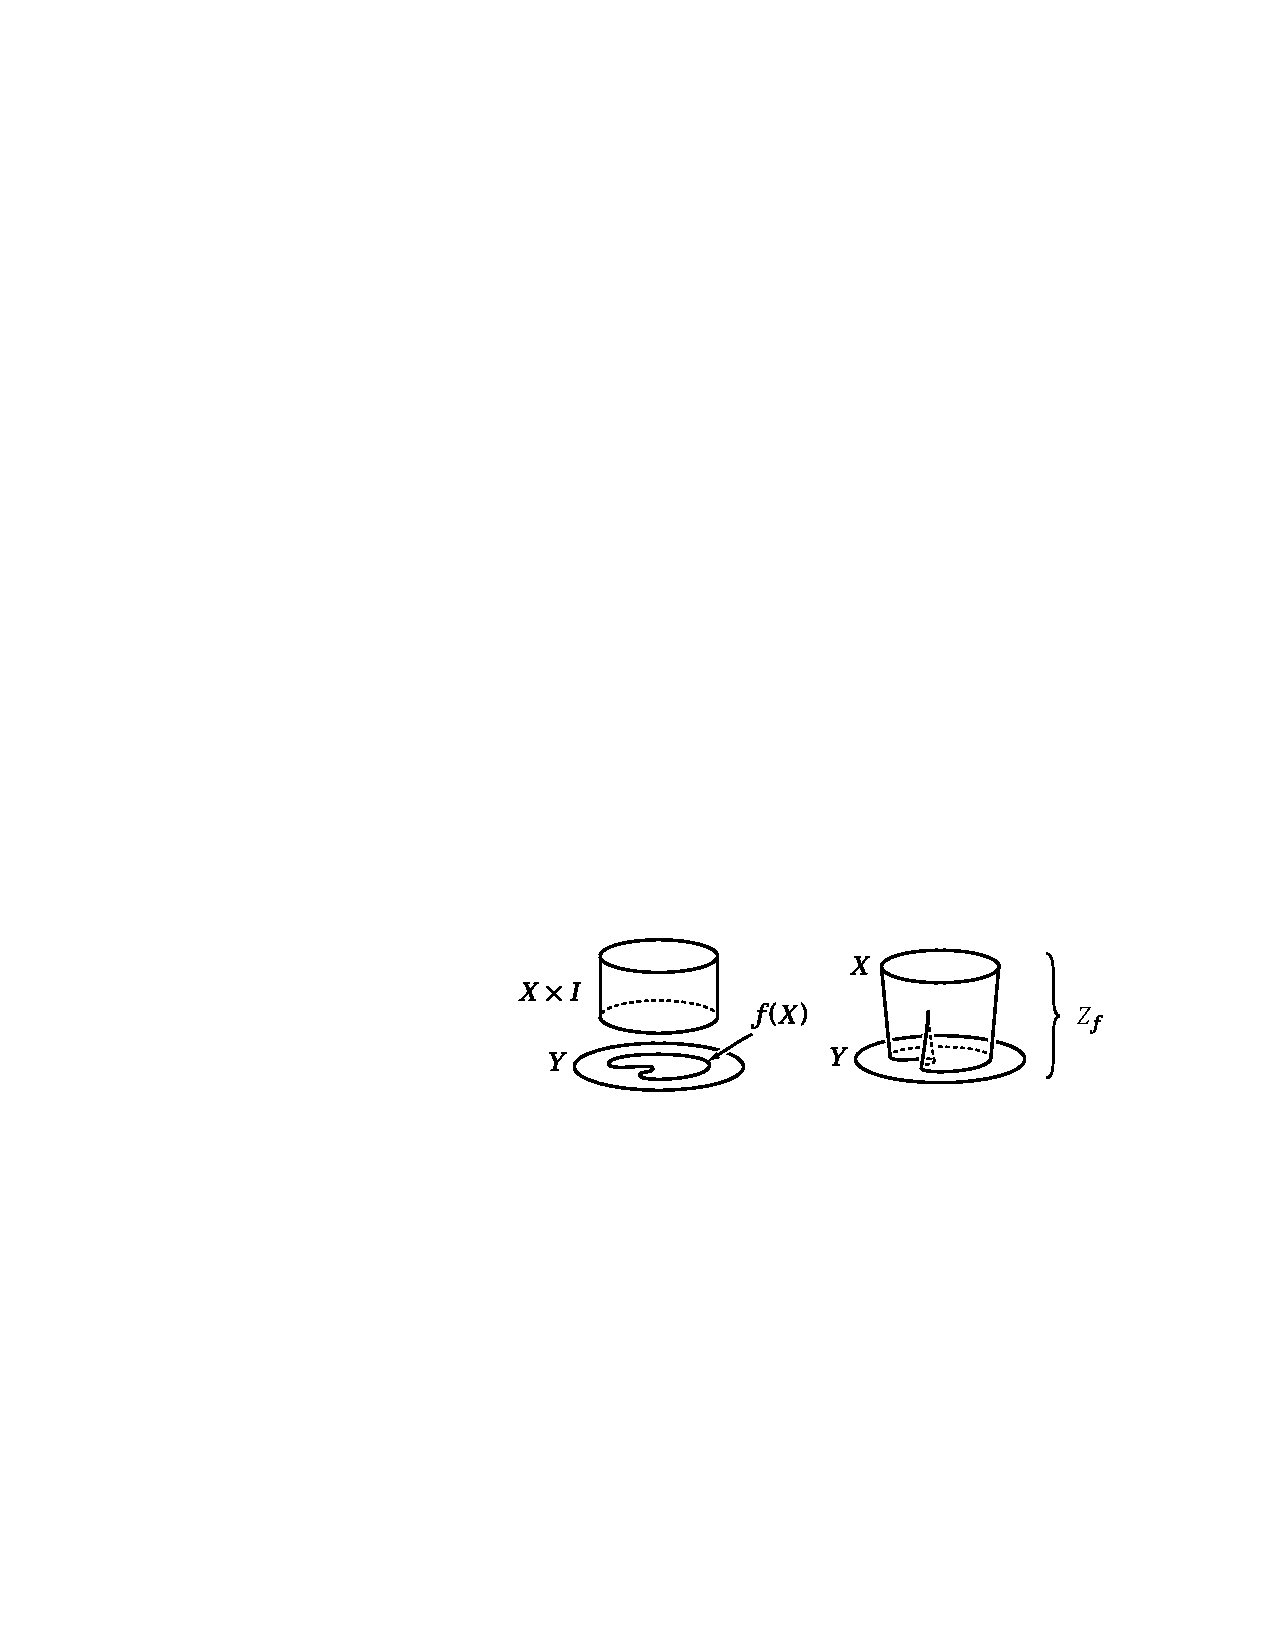
\includegraphics[width=0.5\textwidth]{Images/cylinder.pdf}
    \caption{Mapping cylinder of $f$.}
    \label{fig:mapping cyl}
\end{figure}

\begin{defn}[Mapping cylinder]\index{Mapping cylinder}
    Let $f:X\to Y$ be a map. The mapping cylinder of $f$ is the pushout $Z_f$, see Figure~\ref{fig:mapping cyl}, defined as the quotient of $(X\times I)\sqcup Y$ that identifies $(x,0)\in X\times I$ with $f(x)\in Y$:
    \[
    \begin{tikzcd}[every matrix/.append style={name=m}, row sep=large, column sep=large]
       X \sqcup X\arrow[r,"f\sqcup \mathrm{id}"]\arrow[d,"i_0\sqcup i_1",swap] & Y\sqcup X\arrow[d,"s\sqcup j"]\\
       X\times I \arrow[r,"a", swap] & Z_f
    \end{tikzcd}, \;
    \begin{matrix}
        Z_f=\bigslant{(X\times I)\sqcup Y}{(x,0)\sim f(x)},\\
        s(y)=y,\; j(x)=(x,1), \\ i_0(x)=(x,0),\; i_1(x)=(x,1).
    \end{matrix}
    \]
    We also have the projection $q:Z_f\to Y$, $(x,t)\mapsto f(x)$, $y\mapsto y$.
\end{defn}

The images $q(X\times\{1\})$ and $q(Y)$ are homeomorphic to $X$ and $Y$ respectively. When $X$ and $Y$ are homotopy equivalent, both of these subspaces of $Z_f$ can be shown to be deformation retracts of $Z_f$. Therefore two spaces $X,Y$ are homotopy equivalent iff they are homeomorphic to deformation retracts of some third space $Z$. See e.g.\ \cite[Prop.~7.46]{LeeTop} for a proof. We will also provide a proof in Corollary~\ref{cor 0.21 Hatcher}.


\begin{figure}
    \centering
    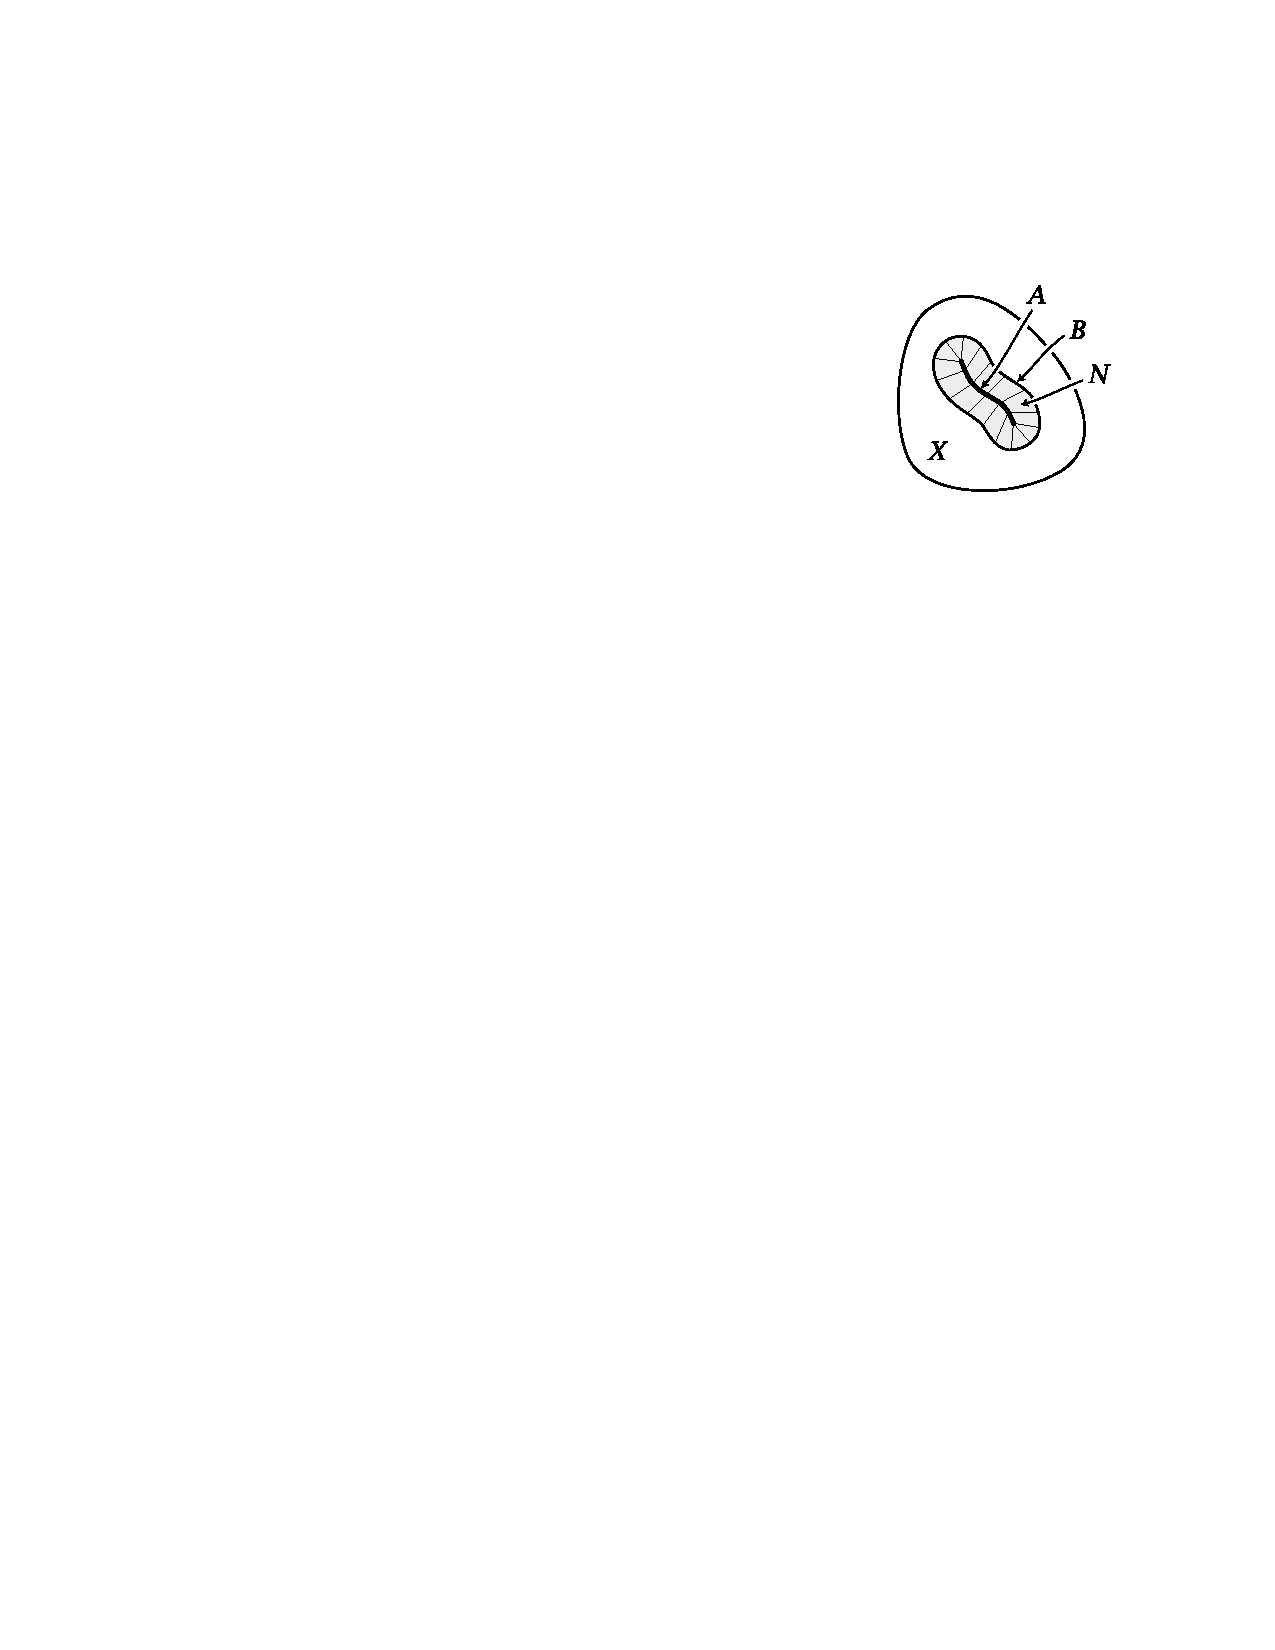
\includegraphics[width=0.3\textwidth]{Images/hep_example.pdf}
    \caption{Mapping cylinder neighborhood from Example~\ref{example Z_f hep}.}
    \label{fig: Z_f hep}
\end{figure}
\begin{example}\label{example Z_f hep}
    A pair $(X,A)$ has the \gls{hep} if $A$ has a mapping cylinder neighborhood of $X$, by which we mean a closed neighborhood $N$ containing a subspace $B$, thought of as the boundary of $N$, with $N\setminus B$ an open neighborhood of $A$, such that there exists a map $f:B\to A$ and a homeomorphism $h:Z_f\to N$ with $\restr{h}{A\cup B}=\id$. Mapping cylinder neighborhoods like this occur fairly often. For example thickened graphs in the plane, see Figure~\ref{fig: Z_f hep}.
\end{example}

\begin{xca}
    Show that the mapping cylinder of the double covering map $\pi$ of the circle $\bbS^1$ ($\pi(z)=z^2$ on the unit circle in $\bbC$) is homeomorphic to a bounded M\"obius band.
\end{xca}


\begin{prop}[{{\cite[Prop.~0.16]{Hatcher}}}]\label{prop 0.16 Hatcher}
    If $(X,A)$ is a $CW$ pair (i.e.~$A$ is a subcomplex of $X$), then $(X\times\{0\})\cup (A\times I)$ is a deformation retract of $X\times I$, hence $(X,A)$ is a cofibration.
\end{prop}
\begin{proof}
    There is a retraction $r:\bbD^n\times I\to (\bbD^n\times\{0\})\cup (\partial \bbD^n\times I)$, for example the radial projection from the point $(0,2)\in \bbD^n\times \bbR$. Then setting $r_t=t\cdot r+(1-t)\id$ gives a deformation retraction of $\bbD^n\times I$ onto $(\bbD^n\times\{0\})\cup (\partial \bbD^n\times I)$. This deformation gives rise to a deformation retraction of $X^{(n)}\times I$ onto $(X^{(n)}\times\{0\})\cup ((X^{(n-1)}\cup A^{(n)})\times I)$ since $X^{(n)}$ is obtained from the latter by attaching copies of $\bbD^n\times I$ along $(\bbD^n\times\{0\})\cup (\partial \bbD^n\times I)$. If we perform this deformation retraction in dimension $n$ during the $t$-interval $[2^{-n-1},2^{-n}]$, this infinite concatenation of homotopies is a deformation retraction of $X\times I$ onto $(X\times\{0\})\cup (A\times I)$. There is no problem with continuity of this deformation at $t=0$ since it is continuous on $X^{(n)}\times I$, being stationary there during the $t$-interval $[0,2^{-n-1}]$, and $CW$-complexes have the weak topology with respect to their skeleta so a map is continuous iff its restriction to each skeleton is continuous.
\end{proof}

\begin{prop}[{{\cite[Prop.~0.17]{Hatcher}}}]
    If the pair $(X,A)$ is a cofibration and $A$ is contractible, then the quotient map $q:X\to X\slash A$ is a homotopy equivalence.
\end{prop}
\begin{proof}
    We can use the \gls{hep} to extend a contraction of $A$ to a homotopy of maps $X\to X$ that map $A$ to $A$. This descends to a homotopy of maps $X\slash A\to X\slash A$. At $t=1$ this homotopy produces a map that maps $A$ to the point to which $A$ was contracted, so this map induces a map $X\slash A\to X$. It is then easy to see that this map is a homotopy inverse of $q$ via the two homotopies constructed above.
\end{proof}

\begin{prop}[{{\cite[Prop.~0.18]{Hatcher}}}]
    If $(X_1,A)$ is a $CW$-pair and we have the attaching maps $f,g:A\to X_0$ that are homotopic, then $X_0\sqcup_f X_1\simeq X_0\sqcup_g X_1 \rel X_0$.
\end{prop}
\begin{proof}
    If $F:A\times I\to X_0$ is the homotopy from $f$ to $g$, then consider the space $X_0\sqcup_F (X_1\times I)$. This contains both spaces in the claim of the theorem as subspaces. A deformation retraction of $X_1\times I$ onto $(X_1\times \{0\})\cup (A\times I)$ as in Proposition~\ref{prop 0.16 Hatcher} induces a deformation retraction of $X_0\sqcup_F (X_1\times I)$ onto $X_0\sqcup_f X_1$. Similarly that space retracts onto $X_0\sqcup_g X_1$. Both of these deformation retractions restrict to the identity map on $X_0$, so they give the necessary homotopy equivalence.
\end{proof}

\begin{prop}[{{\cite[Prop.~0.19]{Hatcher}}}]
    Suppose $(X,A)$ and $(Y,A)$ are cofibrations and $f:X\to Y$ is a homotopy equivalence with $\restr{f}{A}=\id_A$. Then $f$ is a homotopy equivalence $\rel A$.
\end{prop}
\begin{proof}
    We only outline the proof, see \cite[Prop.~0.19]{Hatcher} for the full details. Let $g:Y\to X$ be a homotopy inverse of $f$. The idea is to construct a homotopy from $g$ to a map $g_1$ such that $\restr{g_1}{A}=\id_A$. This is possible by taking the existing homotopy from $g\circ f$ to $\id_X$, restricting it to a homotopy from $\restr{g}{A}$ to $\id_A$, and extending it to a homotopy of maps $Y\to X$. At $t=1$ this homotopy will give the necessary $g_1$. Then we check that $g_1\circ f\simeq \id_X \,\rel A$ and that $f\circ g_1\simeq \id_Y\,\rel A$.  
\end{proof}
By applying the above to the inclusion map we immediately get the next Corollary.
\begin{cor}[{{\cite[Cor.~0.20]{Hatcher}}}]
    If $(X,A)$ is a cofibration and the inclusion $i:A\hookrightarrow X$ is a homotopy equivalence, then $A$ is a deformation retract of $X$.
\end{cor}
\begin{cor}[{{\cite[Cor.~0.21]{Hatcher}}}]\label{cor 0.21 Hatcher}
    A map $f:X\to Y$ is a homotopy equivalence iff $X$ is a deformation retract of the mapping cylinder $Z_f$. Hence, two spaces $X\simeq Y$ iff there is a third space containing both $X$ and $Y$ as deformation retracts.
\end{cor}
\begin{proof}
    We have the inclusions $i:X\hookrightarrow Z_f$ and $j:Y\hookrightarrow Z_f$, and the canonical retraction $r:Z_f\to Y$, so $f=r\circ i$ and $i\simeq j\circ f$. Since $j$ and $r$ are homotopy equivalences (``h.e.''), it follows that $f$ is a h.e.\ iff $i$ is h.e., since the composition of two h.e.'s\ is a h.e.\ and a map homotopic to a h.e.\ is also a h.e. Now we apply the preceding Corollary to the pair $(Z_f,X)$, which is a cofibration by Example~\ref{example Z_f hep} using the neighborhood $X\times [0,\frac12]$ of $X$ in $Z_f$.
\end{proof}





\subsection{Whitehead's theorem}

Let us first adapt the Compression Criterion (Proposition~\ref{prop: compression criterion}) to the context of $CW$-complexes.

\begin{lem}[Compression Lemma]\index{Lemma!compression}
    Let $(X,A)$ be a $CW$ pair (i.e.~$A$ is a subcomplex of $X$) and let $(Y,B)$ be any pair with $B\neq\varnothing$. For each $n$ such that $X\setminus A$ has cells of dimension $n$, assume that $\pi_n(Y,B,y_0)=0$ for all $y_0\in B$. Then every map $f:(X,A)\to (Y,B)$ is homotopic $\rel A$ to a map $X\to B$.

    When $n=0$ the condition $\pi_n(Y,B,y_0)=0$ for all $y_0\in B$ is to be regarded as saying that $(Y,B)$ is connected.
\end{lem}
\begin{proof}
    Assume inductively that $f$ has already been homotoped to take the skeleton $X^{(k-1)}$ to $B$. If $\Phi$ is the characteristic map of a $k$-cell $e^k$ of $X\setminus A$, the composition $f\circ \Phi:(\bbD^k,\partial \bbD^k)\to (Y,B)$ can be homotoped into $B$ $\rel \partial \bbD^k$ in view of the hypothesis that $\pi_k(Y,B,y_0)=0$ if $k>0$, or that $(Y,B)$ is $0$-connected if $k=0$. This homotopy of $f\circ\Phi$ induces a homotopy of $f$ on the quotient space $X^{(k-1)}\cup e^k$ of $X^{(k-1)}\sqcup \bbD^k$, a homotopy $\rel X^{(k-1)}$. Doing this for all $k$-cells of $X\setminus A$ simultaneously, and taking a constant homotopy on $A$, we obtain a homotopy of $\restr{f}{X^{(k)}\cup A}$ to a map into $B$. By the homotopy extension property, this homotopy extends to a homotopy defined on all of $X$, and the induction step is completed.

    Finitely many applications of the induction step finish the proof if the cells of $X\setminus A$ are bounded in dimension. Otherwise, we can perform the homotopy of the induction step during the $t$-interval $[1-2^{-k},1-2^{-k-1}]$. Any finite skeleton $X^{(k)}$ is eventually stationary under these homotopies, hence we have a well-defined homotopy $f_t$, $t\in [0,1]$ with $f_1(X)\subset B$.
\end{proof}


\begin{thm}[Whitehead's Theorem]\index{Theorem!Whitehead}\label{thm whitehead}
    If a map $f:X\to Y$ between connected $CW$-complexes induces isomorphisms $f_\ast :\pi_n(X)\to \pi_n(Y)$ for all $n$, then $f$ is a homotopy equivalence. 
    
    If $f$ is the inclusion map of a subcomplex $X\hookrightarrow Y$, the conclusion is stronger: $X$ is a deformation retract of $Y$.
\end{thm}
\begin{proof}
    In the special case that $f$ is the inclusion of a subcomplex, consider the long exact sequence on all homotopy groups of $(Y,X)$. Since $f$ induces isomorphisms of all homotopy groups, the relative groups $\pi_n(Y,X)$ are zero. Applying the Compression Lemma to the identity map on $(Y,X)$ then yields a deformation retraction of $Y$ onto $X$.

    The general case can be proved using mapping cylinders. Recall that the mapping cylinder $Z_f$ is the quotient space of the disjoint union of $X\times I$ and $Y$ under the identifications $( x, 1 ) \sim f ( x )$. Thus $Z_f$ contains both $X = X\times { 0 }$ and $Y$ as subspaces, and $Z_f$ deformation retracts onto $Y$. The map $f$ becomes the composition of the inclusion $X\hookrightarrow Z_f$ with the retraction $Z_f\to Y$. Since this retraction is a homotopy equivalence, it suffices to show that $Z_f$ deformation retracts onto $X$ if $f$ induces isomorphisms on homotopy groups, or equivalently, if the relative groups $\pi_n(Z_f,X)$ are all trivial.

    If the map $f$ happens to be \emph{cellular}\index{Cellular map}, i.e.~taking $X^{(n)}$ to $Y^{(n)}$, then $(Z_f,X)$ is a $CW$-pair and so we are done by the first paragraph of the proof. If $f$ is not cellular, we can either appeal to the Cellular Approximation Theorem~\ref{thm cell approx} which says that $f$ is homotopic to a cellular map, or use the following argument. First apply the Compression Lemma to obtain a homotopy $\rel X$ of the inclusion $(X\cup Y,X)\hookrightarrow (Z_f,X)$ to a map into $X$. Since the pair $(Z_f,X\cup Y)$ obviously is a cofibration, this homotopy extends to a homotopy from $\id_{Z_f}$ to a map $g:Z_f\to Z_f$ taking $X\cup Y$ into $X$. Then apply the Compression Lemma again to the composition $((X\times I)\sqcup Y,(X\times\partial I)\sqcup Y)\to (Z_f,X\cup Y)\overset{g}{\to} (Z_f,X)$ to finish the construction of a deformation retraction of $Z_f$ onto $X$.
\end{proof}

\begin{rem}
    The Whitehead theorem \emph{does not} say that two complexes with isomorphic homotopy groups are homotopy equivalent -- the existence of a map $f$ that generates those isomorphisms is crucial! For example, $\bbR P^2$ and $\bbS^2\times \bbR P^\infty$ both have fundamental group $\bbZ_2$ and trivial higher groups (since their universal covers $\bbS^2$ and $\bbS^2\times \bbS^\infty$ are homotopy equivalent,  $\bbS^\infty$ being contractible). But these two spaces are not homotopy equivalent because they have vastly different homology groups.
\end{rem}

\begin{defn}[Weak homotopy equivalence]
    A map $f:X\to Y$ is called a weak homotopy equivalence if all the induced homomorphisms $f_\ast:\pi_n(X,*)\to \pi_n(Y,*)$, $n\geq 0$, are isomorphisms regardless of the choice of basepoints.
\end{defn}


Whitehead's theorem therefore states that a weak homotopy equivalence between $CW$-complexes is actually a homotopy equivalence.  In general, however, weak homotopy equivalences are a much bigger class of maps. For example, there exist noncontractible spaces whose homotopy groups are all trivial, such as the `quasi-circle'. For such spaces a map to a point is a weak homotopy equivalence that but not a homotopy equivalence. 

One special case where isomorphisms by themselves do imply homotopy equivalence is when all homotopy groups are trivial.

\begin{defn}[Weakly contractible space]\index{Weakly contractible space}
    A space $X$ is called weakly contractible if $\pi_n(X)$ is trivial for all $n\geq 0$.
\end{defn}

\begin{cor}
    A weakly contractible $CW$-complex is contractible.
\end{cor}
\begin{proof}
    The inclusion map of a $0$-cell into the complex induces an isomorphism of the trivial homotopy groups, therefore by Whitehead's theorem there is a homotopy equivalence with a point.
\end{proof}

\begin{lem}[Extension Lemma]\label{lem 4.7 Hatcher}
    Let $(X,A)$ be a $CW$-pair and $Y$ is a path-connected space such that $\pi_{n-1}(Y)=0$ for all $n$ in which $X^{(n)}\setminus A^{(n)}\neq \varnothing$. Then any continuous map $f:A\to Y$ can be extended to a map $\wt f:X\to Y$.
\end{lem}
\begin{proof}
    Assume $f$ was already extended to a map $f^{(n-1)}$ over the $(n-1)$-skeleton. Then an extension over all $n$-cells exists iff the composition of the cell's attaching map $\bbS^{n-1}\to X^{(n-1)}$ with $f^{(n-1)}$ is nullhomotopic.
\end{proof}





\subsection{Cellular approximation}


Recall when we applied the van Kampen theorem to compute $\pi_1(\bbS^n)=0$ for $n\geq 2$, we implicitly used the fact that every loop can be deformed to miss at least one point in $\bbS^n$, and then it can obviously be contracted to a point since $\bbS^n\setminus *$ is contractible. This is not an obvious fact since there exist space-filling loops that are surjective. Similar space-filling maps exist for all pairs $\bbS^m\to \bbS^n$ with $m<n$.

For homotopy theory of $CW$ complexes it turns out to be sufficient to work with maps that map $n$-skeleta to $n$-skeleta, and any other map is homotopic to one of this class.



\begin{lem}[{{\cite[Lem.~4.10]{Hatcher}}}]\label{lem 4.10 hatcher}
    Let $f:Y^n\to Z$ be a map, where $Z$ is obtained from a subspace $W$ by attaching a $k$-cell $e^k$. Then there is a homotopy $f_t:(I^n,f^{-1}(e^k))\to (Z,e^k)$ $\rel f^{-1}(W)$ from $f=f_0$ to a map $f_1$ for which there is a polyhedron $K\subset I^n$ such that:
    \begin{enumerate}[label=(\alph*)]
        \item $f_1(K)\subset e^k$ and $\restr{f_1}{K}$ is piecewise linear (i.e.~linear on each face of $K$) with respect to some identification of $e^k$ with $\bbR^n$.
        \item There exists a nonempty open $U\subset e^k$ such that $f_1^{-1}(U)\subset K$.
    \end{enumerate}
\end{lem}
\begin{proof}
    Identifying $e^k$ with $\bbR^k$, let $B_1,b_2\subset e^k$ be the closed balls of radius $1$ and $2$ at the origin. Since $f^{-1}(B_2)$ is closed and therefore compact in $I^n$, it follows that $f$ is uniformly continuous on $f^{-1}(B_2)$. Thus there exists $\epsilon>0$ such that $|x-y|<\epsilon$ implies $|f(x)-f(y)|<\frac 12$ for all $x,y\in f^{-1}(B_2)$. Subdivide the interval $I$ so that the induced subdivision of $I^n$ into cubes has each cube lying in a ball of diameter less than $\epsilon$. Let $K_1$ be the union of all the cubes meeting $f^{-1}(B_1)$ and let $K_2$ be the union of all cubes meeting $K_1$. We may assume $\epsilon$ is chosen smaller than half the distance between the compact sets $f^{-1}(B_1)$ and $I^n\setminus f^{-1}(\int B_2)$, and then we will have $K_2\subset f^{-1}(B_2)$. See Figure~\ref{fig:cell_approx}.

    Now we subdivide all the cubes of $K_2$ into simplices. This can be done inductively in the dimension by taking the center point of a cube as a new vertex and joining it by a cone to each simplex in boundary of the cube. 

    Let $g:K_2\to e^k=\bbR^k$ be the map that equals $f$ on all vertices of simplices of the subdivision and is linear on each simplex. Let $\varphi:K_2\to [0,1]$ be the map that is linear on simplices and has value $1$ on vertices in $K_1$ and $0$ on vertices of $K_2\setminus K_1$. Thus $\restr{\varphi}{K_1}=1$. Define a homotopy $f_t:K_2\to e^k$ by the formula $(1-t\varphi)\cdot f+(t\varphi)\cdot g$, so $f_0=f$ and $\restr{f_1}{K_1}=\restr{g}{K_1}$. Since $f_t$ is constant in $t$ on simplices in $K_2$ disjoint from $K_1$, and in particular on simplices in the closure $\widebar{I^n\setminus K_2}$, we may extend $f_t$ to be the constant homotopy of $f$ on $I^n\setminus K_2$.

    The map $f_1$ takes the closure $\widebar{I^n\setminus K_1}$ to a compact set $C$ which, we claim, is disjoint from the center $0$ of $B_1$ and hence from a neighborhood $U$ of $0$. This will prove the lemma, with $K=K_1$ since we will have $f_1^{-1}(U)\subset K_1$ with $f_1$ piecewise linear on $K_1$ where it is equal to $g$.

    The verification of the claim has two steps:
    \begin{enumerate}[label=(\arabic*)]
        \item On $I^n\setminus K_2$ we have $f_1=f$, and $f$ takes $I^n\setminus K_2$ outside $B_1$ since $f^{-1}(B)\subset K_2$ by construction.
        \item For a simplex $\sigma$ of $K_2$ not in $K_1$ we have $f(\sigma)$ contained in some ball $B_\sigma$ of radius $\frac 12$ by the choice of $\epsilon$ and the fact that $K_2\subset f^{-1}(B_2)$. Since $B_\sigma$ is convex, we must also have $g(\sigma)\subset B_\sigma$. We know that $g(\sigma)\subset B_\sigma$, hence also $f_t(\sigma)\subset B_\sigma$ for all $t$, and in particular $f_1(\sigma)\subset B_\sigma$. We know that $B_\sigma\cancel{\subset} B_1$ since $\sigma\cancel{\subset}K_1$ and thus $\sigma\cancel{\subset}f^{-1}(B_1)$. The radius of $B_\sigma$ is half that of $B_1$, so it follows that $0\notin B_\sigma$, and hence $0\notin f_1(\sigma)$.
    \end{enumerate}
\end{proof}

\begin{figure}
    \centering
    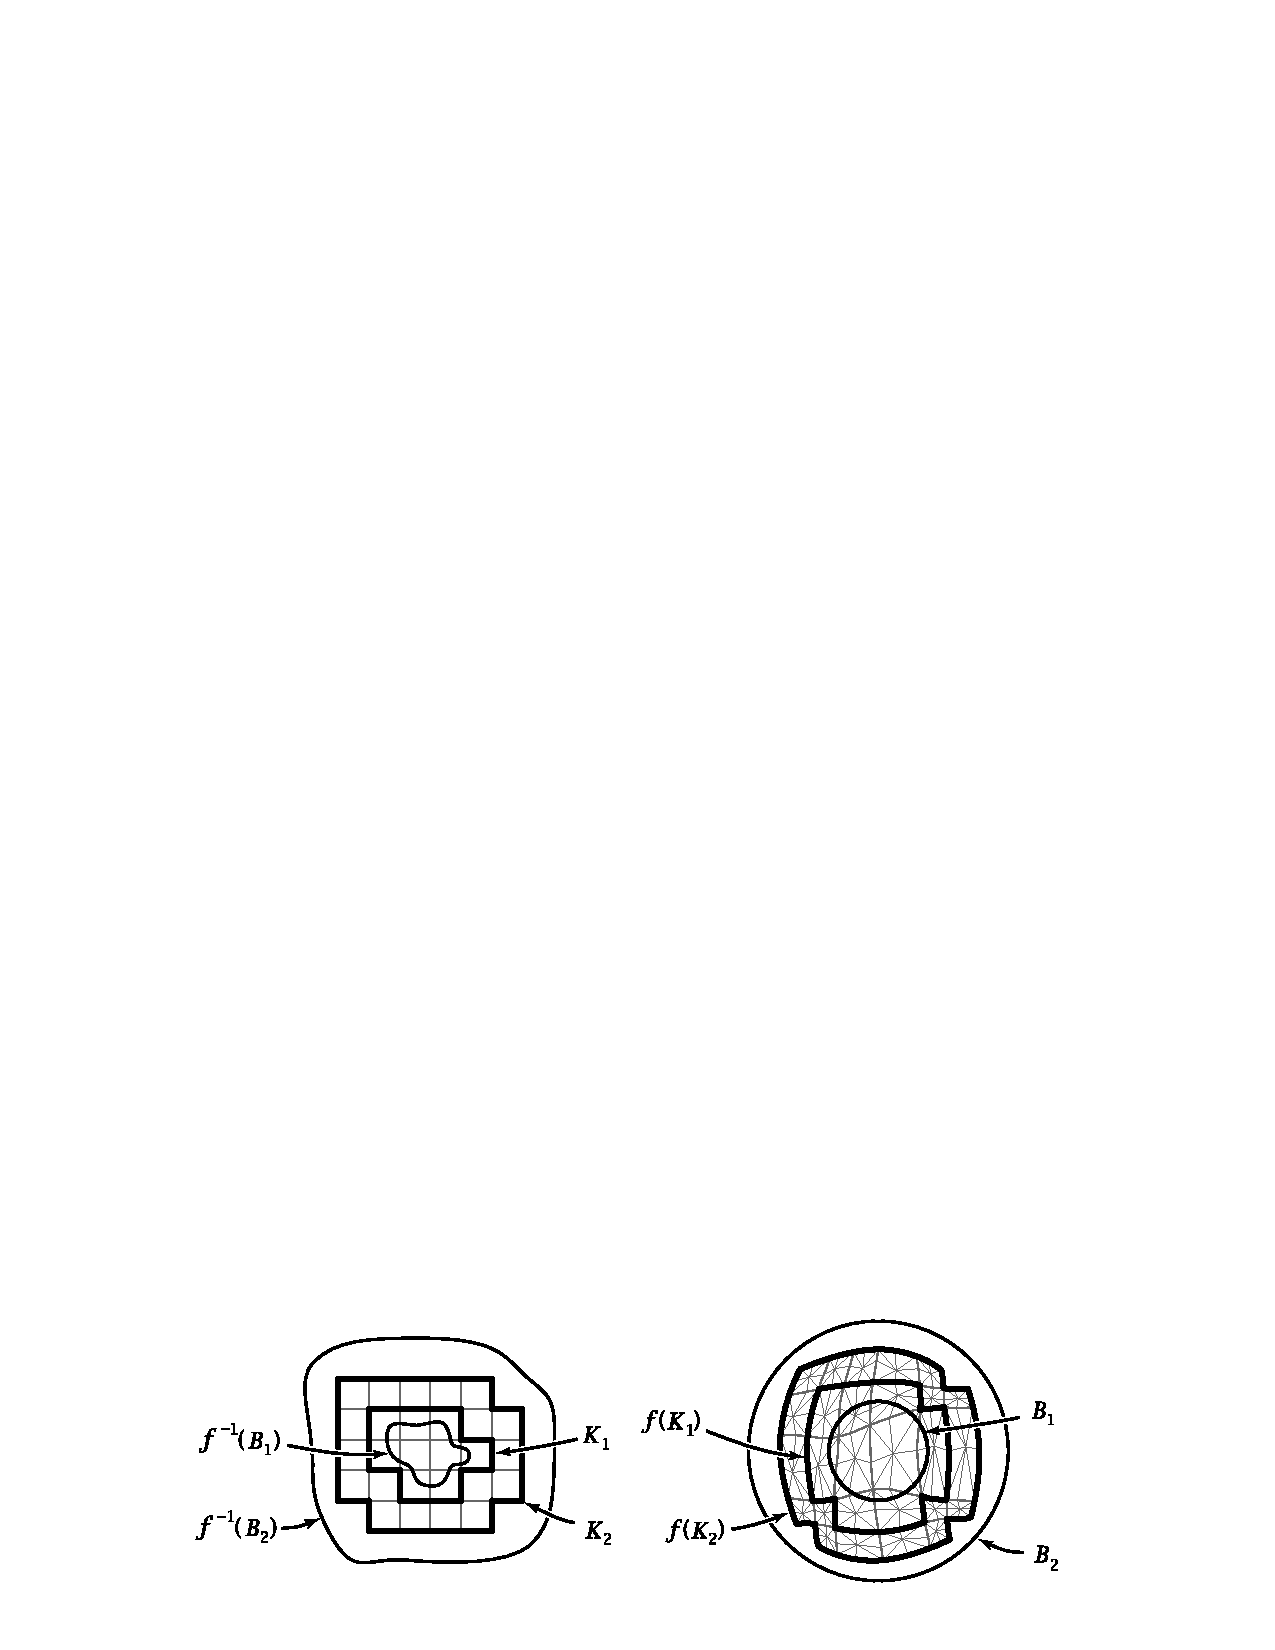
\includegraphics[width=0.7\textwidth]{Images/cell_approx.pdf}
    \caption{Subdivision from the proof of Lemma~\ref{lem 4.10 hatcher}.}
    \label{fig:cell_approx}
\end{figure}


\begin{thm}[Cellular Approximation Theorem]\index{Theorem!Cellular Approximation}\label{thm cell approx}
    Every map $f:X\to Y$ of $CW$-complexes is homotopic to a cellular map. 

    Every map $f:(X,A)\to (Y,B)$ of $CW$-pairs is homotopic $\rel A$ to a cellular map.
\end{thm}
\begin{proof}
    Suppose inductively that $f$ is cellular on $X^{(n-1)}$, and let $e^n$ be an $n$-cell of $X$. The closure of $e^n$ in $X$ is compact, being the image of a characteristic map for $e^n$ (Proposition~\ref{prop f(compact)=compact}), so $f$ takes the closure of $e^n$ to a compact set in $Y$.  Therefore $f(e^n)$ meets finitely many cells of $Y$.  Let $e^k\subset Y$ be a cell of highest dimension meeting $f(e^n)$. We may assume $k>n$, otherwise $f$ is already cellular on $e^n$.

    Now we apply Lemma~\ref{lem 4.10 hatcher} to the composition of $f:X^{(n-1)}\cup e^n\to Y^{(k)}$ with a characteristic map $I^n\to X$ for $e^n$, with $Z=Y^{(k)}$ and $W=Y^{(k)}\setminus e^k$. The homotopy given by the lemma is fixed on $\partial I^n$, hence induces a homotopy $f_t$ of $\restr{f}{X^{(n-1)}\cup e^n}$ fixed on $X^{(n-1)}$. The image of the resulting map $f_1$ intersects the open set $U\subset e^k$ in a set contained in the union of finitely many hyperplanes of dimension at most $n$, so if $n<k$ there will be points $p\in U$ not in the image of $f_1$. 
    
    In summary, it is possible to deform $\restr{f}{X^{(n-1)}\cup e^n}$, staying fixed on $X^{(n-1)}$, so that $f(e^n)$ misses some point $p\in e^k$. Then we can deform $\restr{f}{X^{(n-1)}\cup e^n}$ $\rel X^{(n-1)}$ so that $f(e^n)$ misses the whole cell $e^k$ by composing with a deformation retraction of $Y^{(k)}\setminus \{p\}$ onto $Y^{(k)}\setminus e^k$. By finitely many iterations of this process we eventually make $f(e^k)$ miss all cells of dimension greater than $n$. Doing this for all $n$-cells simultaneously, staying fixed on $n$-cells in $A$ where $f$ is already cellular, we obtain a homotopy of $\restr{f}{X^{(n)}}$ $\rel X^{(n-1)}\cup A^{(n)}$ to a cellular map. 

    The induction step is then completed by appealing to the \gls{hep} in Proposition~\ref{prop 0.16 Hatcher} to extend this homotopy, together with the constant homotopy on $A$, to a homotopy defined on all of $X$. Letting $n$ go to infinity, the resulting possibly infinite sequence of homotopies can be realized as a single homotopy by performing the $n$-th homotopy during the $t$-interval $[1-2^{-n},1-2^{-n-1}]$. This homotopy will eventually be stationary on every $k$-skeleton and hence continuous at $1$.
\end{proof}

\begin{cor}\label{cor pi_n(S^k)=0}
    $\pi_n(\bbS^k)=0$ for $n<k$.
\end{cor}
\begin{proof}
    If $\bbS^n$ and $\bbS^k$ are given $CW$ structures with one $0$-cell (serving as as basepoint) and one $n(k)$-cell, then every pointed map $\bbS^n\to \bbS^k$ can be homotoped, fixing the basepoint, to be cellular, and hence constant if $n<k$.
\end{proof}





\subsection{\texorpdfstring{$CW$}{CW} approximation}\label{sec: CW approx}

Whitehead's theorem obviously holds not just for $CW$-complexes, but also for spaces that are homotopy equivalent to them. We now show that any topological space is \emph{weakly} homotopy equivalent to a $CW$-complex.

\begin{defn}[$CW$ approximation]
    A $CW$ approximation of a topological space $X$ is a $CW$-complex $Z$ with a weak homotopy equivalence $f:Z\to X$.
\end{defn}

\begin{prop}[{{\cite[Prop.~4.13]{Hatcher}}}]
    Every space $X$ has a $CW$ approximation $f:Z\to X$. If $X$ is path-connected, $Z$ can be chosen to have a single $0$-cell, with all other cells attached by pointed maps. Thus every connected $CW$-complex is homotopy equivalent to a $CW$-complex with these additional properties.
\end{prop}
\begin{proof}
    The construction of a $CW$ approximation $f:Z\to X$ for a space $X$ is inductive. Suppose given a $CW$-complex $A$ with a map $f:A\to X$ and suppose we have chosen a basepoint $0$-cell $*$ in each component of $A$. Then for an integer $k\geq 0$ we will attach $k$-cells to $A$ to form a $CW$ complex $B$ with a map $f:B\to X$ extending the given $f$, such that the induced homomorphism $f_\ast:\pi_i(B,*)\to \pi_i(X,f(*))$ is injective for $i=k-1$ and surjective for $i=k$, for all basepoints $*$.

    There are two steps:
    \begin{enumerate}[label=(\arabic*)]
        \item Choose maps $\varphi_\alpha:(\bbS^{k-1},s_0)\to (A,*)$ representing a set of generators for the kernel of $f_\ast:\pi_{k-1}(A,*)\to \pi_{k-1}(X,f(*))$ for all basepoints $*$. We map assume the maps $\varphi_\alpha$ are cellular, where $\bbS^{k-1}$ has its standard $CW$ structure with $s_0$ as the $0$-cell. Attaching cells $e_\alpha^k$ to $A$ via $\varphi_\alpha$ then produces a $CW$ complex, and the map $f$ extends over these cells using nullhomotopies of $f\circ \varphi_\alpha$, which exist by the choice of the $\varphi_\alpha$'s.
        \item Choose maps $f_\beta:\bbS^k\to X$ representing generators for the groups $\pi_k(X,f(*))$, attach cells $e_\beta^k$ to $A$ via the constant maps at the appropriate basepoints $*$, and extend $f$ over the resulting spheres $S_\beta^k$ via the $f_\beta$'s.
    \end{enumerate}

    The surjectivity of $f_\ast$ holds by construction. For the injectivity, an element of the kernel of $f_\ast:\pi_{k-1}(B,*)\to \pi_{k-1}(X,f(*))$ can be represented by a cellular map $h:\bbS^{k-1}\to B$. This has image in $A$, so is in the kernel of $f_\ast:\pi_{k-1}(A,*)\to \pi_{k-1}(X,f(*))$ and hence is homotopic to a linear combination of the $\varphi_\alpha$'s, which are nullhomotopic in $B$, so $h$ is nullhomotopic as well. When $k=1$ there is no group structure on $\pi_{k-1}$ so injectivity on $\pi_0$ does not follow from having a trivial kernel, and we modify the construction by choosing the cells $e_\alpha^1$ to join each pair of basepoints $*$ that map by $f$ to the same path-component of $X$. The map $f$ can then be extended over these $1$-cells $e_\alpha^1$.

    Note that if $f$ happened to be injective or surjective on $\pi_i$ for some $i<k-1$ or $i<k$, respectively, then this remains true after attaching the $k$-cells. This is because attaching $k$-cells does not affect $\pi_i$ if $i<k-1$, by cellular approximation, not does it destroy surjectivity on $\pi_{k-1}$ or indeed any $\pi_i$, obviously.

    Now to construct a $CW$ approximation $f:Z\to X$ one can start with $A$ consisting of one point for each path-component of $X$, with $f:A\to X$ mapping each of them to the corresponding path-component. Having now a bijection on $\pi_0$, attach $1$-cells to $A$ to create a surjection on $\pi_1$  for each path-component, then $2$-cells to improve this to an isomorphism on $\pi_1$ and a surjection on $\pi_2$, and so on for each successive $\pi_i$. After all cells have been attached one has a $CW$-complex $Z$ and a weak homotopy equivalence $f:Z\to X$.
\end{proof}

\begin{rem}
    One can apply this technique to produce $CW$ approximations of pairs $(X,A)$. First construct a $CW$ approximation $f_A:Z_A\to A$, then starting with the composition $Z_A\to A\hookrightarrow X$, attach cells to $Z_A$ to create a weak homotopy equivalence $f:Z\to X$ extending $f_A$. The induced map $f_\ast$ will be an isomorphism of relative homotopy groups  by the five-lemma~\ref{5-lemma} applied to the two sequences of morphisms in relative and absolute homotopy.
\end{rem}


Running ahead, we will be calling a $CW$-pair $(Z,A)$ \emph{$n$-connected} if $\pi_k(Z,A,a)=0$ for $k=1,\ldots n$ and all $a\in A$, and the inclusion-induced map $\pi_0(A)\to \pi_0(Z)$ is surjective. 

\begin{defn}[$n$-connected $CW$ model]
    An $n$-connected $CW$ model for a $CW$ pair $(X,A)$ with a nonempty subcomplex $A$ is an $n$-connected $CW$ pair $(Z,A)$ and a map $f:Z\to X$ with $\restr{f}{A}=\id_A$ such that the induced homomorphism $f_\ast:\pi_i(Z)\to \pi_i(X)$ is an isomorphism for $i>n$ and an injection for $i=n$, for all choices of basepoint.
\end{defn}

One can think of $Z$ as a homotopy-theoretic hybrid of $X$ and $A$. As $n$ increases it looks more and more like $A$, and less like $X$. We have just shown that $n$-connected models always exist, and can be obtained from $A$ by attaching cells in dimensions $>n$ so that by cellular approximation $(Z,A)$ is $n$-connected. Moreover, it is not difficult to show (\cite[Prop.~4.18, Cor.~4.19]{Hatcher}) that these models (and therefore $CW$ approximations as well) are unique up to homotopy equivalence $\rel A$. In particular, $CW$ approximations are unique up to homotopy equivalence.



\begin{example}[Postnikov towers]
    We can use this technique to construct, for each connected $CW$-complex $X$, and each $n\geq 1$, a $CW$-complex $X_n$ containing $X$ as a subcomplex such that:
    \begin{enumerate}[label=(\alph*)]
        \item $\pi_i(X_n)=0$ for $i>n$;
        \item The inclusion $X\hookrightarrow X_n$ induces an isomorphism on $\pi_i$ for $i\leq n$.
    \end{enumerate}
    To do this, apply the general construction to the constant map of $X$ to a point, starting at the stage of attaching cells of dimension $n+2$. Thus we attach $(n+2)$-cells to $X$ using cellular maps $\bbS^{n+1}\to X$ that generate $\pi_{n+1}(X)$ to form a space with trivial $\pi_{n+1}$, then for this space we attach $(n+3)$-cells to make $\pi_{n+2}$ trivial, and so on. The result is a complex $X_n$ with the desired properties.

    The inclusion $X\hookrightarrow X_n$ extends to a map $X_{n+1}\to X_n$ since $X_{n+1}$ is obtained from $X$ by attaching cells of dimension at least $n+3$, and $\pi_i(X_n)=0$ for $i>n$ so we can apply the Extension Lemma~\ref{extension lemma}. Thus we have a commutative diagram called a Postnikov tower for X. One can regard the spaces $X_n$ as truncations of $X$ which provide successively better approximations to $X$ as $n$ increases. There is a weak homotopy equivalence between $X$ and the inverse limit of the Postnikov tower $\limit X_n$, i.e.~$X$ is a $CW$ approximation of $\limit X_n$.
    \[
    \begin{tikzcd}[every matrix/.append style={name=m}]
       & \vdots \arrow[d]\\
       & X_3 \arrow[d]\\
       & X_2 \arrow[d]\\
       X\arrow[r]\arrow[ur]\arrow[uur] & X_1
    \end{tikzcd}
    \]
\end{example}


Now we prove one of the statements announced in Remark~\ref{rem: classifying space for discrete G}. 
\begin{prop}\label{prop X_G}
    For every (discrete) group $G$ there exists a path-connected two-dimensional $CW$-complex $X_G$ such that $\pi_1(X_G)\cong G$.
\end{prop}
\begin{proof}
    Consider a presentation of the group as the quotient of a free group $\<J\>$ by some normal subgroup $\<R\>$ generated by a set of relations $R$. Construct the 1-skeleton $X^{(1)}$ of $X_G$ as a wedge sum of circles $\bigvee_{j\in J}\bbS^1$. Every relation describes a loop in $X^{(1)}$: for example if $ab^{-1}c^2$ is a relation, then the loop is given by going around $a$ once, around $b$ once in the opposite direction, and then twice around $c$. For each relation $r\in R$ take a 2-cell $\bbD^2$ with boundary $\bbS^{1}$ and define an attaching map $\varphi_r:\bbS^1\to X^{(1)}$ so that it represents the loop specified by $r$. The resulting $CW$-complex $X_G=X^{(2)}_G$ is then a 2-dimensional complex whose fundamental group is, by construction, isomorphic to $G$.
\end{proof}
We will eventually incorporate this space $X_G$ as into the so called classifying space $\rmB G$, so $\pi_1(\rmB G)\cong \pi_1(X_G)\cong G$, i.e.\ the inclusion is a weak 1-equivalence. The classifying space $\rmB G$ must have $\pi_{n+1}(\rmB G)\cong \pi_{n}(G)$, so in the case of discrete $G$ this is $\pi_{\geq 2}(\rmB G)\cong 0$. In other words, $\rmB G$ for discrete groups is the first Postnikov truncation of the space $X_G$ we just constructed.


\begin{example}\index{Lens spaces}
    Consider the cyclic group $G=C_n\cong \bbZ\slash n\bbZ$ for some integer $n$. Then $X_G$ is $\bbR P^2$ for $n=2$, and for higher $n$ it is a subcomplex of the lens space with fundamental group $C_n$.
\end{example}

\begin{defn}[Aspherical space]\index{Aspherical space}
    A space $X$ is called aspherical if $\pi_n(X)=0$ for all $n\geq 2$.
\end{defn}

\begin{defn}[First Eilenberg-MacLane space]\index{Eilenberg-MacLane space}\label{def: K(G,1)}
    For a group $G$, the first Eilenberg-MacLane space for $G$, denoted $\rmK(G,1)$, is defined up to weak homotopy equivalence as an aspherical space whose fundamental group is $G$. It can be realized as the first Postnikov truncation $(X_G)_1$ of the space $X_G$ constructed in Proposition~\ref{prop X_G}, and in the case of discrete $G$ it coincides with the so called classifying space $\rmB G$. Since $\pi_1$ is the only nontrivial homotopy group of $\rmK(G,1)$, its universal covering space is contractible by Whitehead's theorem.
\end{defn}


\begin{rem}
    We will later be able to define Eilenberg-MacLane and classifying spaces so that they are unique up to homotopy equivalence, not just weak homotopy equivalence. Namely they will be required to be quotients of weakly contractible $CW$-complexes by a free group action, and of course weakly contractible $CW$-complexes are actually contractible by Whitehead's theorem, which will induce a homotopy equivalence between the resulting quotients as well.
\end{rem}


\begin{cor}
    For every discrete group $G$ there exists a (unique up to homotopy equivalence) universal $G$-principal covering $\rmE G\to \rmK(G,1)$ with contractible total space $\rmE G$.
\end{cor}

\begin{example}[Lens spaces {{\cite[Example~2.43]{Hatcher}}}]\index{Lens spaces}\label{example Lens spaces}
    Given an integer $m>1$ and integers $l_1,\ldots,l_n$ relatively prime to $m$, define the lens space $L=L_m(l_1,\ldots,l_n)$ as the orbit space $\bbS^{2n-1}\slash \bbZ_m$ of the unit sphere $\bbS^{2n-1}\subset\bbC^n$ with the action of $\bbZ_m$ generated by the rotation $(z_1,\ldots,z_n)\mapsto (e^{2\pi\rmi l_1/m}z_1,\ldots e^{2\pi\rmi l_n/m} z_n)$. In particular, when $m=2$, for any odd $l_i$'s this is the antipodal map and $L=L_2(1,\ldots,1)=\bbR P^{2n-1}$. In general, the projection $\bbS^{2n-1}\to L$ is a covering space since the action of $\bbZ_m$ is free: each point of $\bbS^{2n-1}$ has at least some coordinate $z_j$ nonzero and then $e^{2\pi\rmi l_j/m}z_j=\neq z_j$ for $0<k<m$ because of the assumption that $l_j$ is relatively prime to $m$.

    One can construct a $CW$-structure on $L$ with one cell in each dimension from $0$ to $2n-1$, see \cite[Example~2.43]{Hatcher}. These structures also induce a $CW$-structure on the infinite lens spaces $L_m(l_1,l_2,\ldots)=\bbS^\infty\slash \bbZ_m$ defined in the same way, which equals the union of the spaces $L_m(l_1,l_2,\ldots,l_n)$ for $n=1,2\ldots$, each of which is a subcomplex of the next. Since the universal covering space $\bbS^\infty$ is contractible, the infinite lens space is an Eilenberg-MacLane space $\rmK(\bbZ_m,1)$.
\end{example}


\begin{xca}\label{xca two definitions of lens spaces}
    Show that the above definition of $L_p(q)$ agrees with the definition of $L(p;q)$ from Example~\ref{example Lens space bredon}. See illustrations \href{https://math.stackexchange.com/a/1186808/31363}{here}. We will give a more direct solution via bundles in Example~\ref{ex monopole bundles}.
\end{xca}










\subsection{Hurewicz fibrations}

\begin{defn}[Hurewicz fibration]\index{Fibration!Hurewicz}
    A continuous map $p:E\to B$ is a (Hurewicz) fibration if it satisfies the \gls{hlp} for \emph{all} spaces $X$. That is, in the diagram (\ref{HLP diagram}) a ``lifted'' homotopy $\wt H$ with initial condition $\wt H(x,0)=\wt H_0(x)$ that makes the diagram commute exists for any space $X$, any homotopy $h:X\times I\to B$, and any continuous $\wt H_0:X\to E$. Here, $i_0$ is the inclusion map $i_0(x)=(x,0)$.
    \[
    \begin{tikzcd}[every matrix/.append style={name=m}, row sep=large, column sep=large]
       X \arrow[r,"\wt H_0"]\arrow[d,"i_0",swap] & E\arrow[d,"p"]\\
       X\times I \arrow[r,"H", swap] \arrow[ur,"\wt H",dashed, swap] & B
    \end{tikzcd} \label{HLP diagram}
    \]
    A morphism between two fibrations $p_1:E_1\to B_2$ and $p_2:E_2\to B_2$ is a pair of continuous maps $f:B_1\to B_2$ and $F:E_1\to E_2$ such that the square formed by them commutes, $p_2\circ F=f\circ p_1$. Such maps are called \emph{fiber-preserving}.
\end{defn}

\begin{example}
    The natural projections in a direct product are fibrations. Indeed, for the projection $\pi:B\times F\to B$ the homotopy lifting problem, defined by a map $f:X\times I\to B$ and an initial condition $\wt{f}_0:X\times\{0\}\to B\times F$, is solved by the map
    \[\wt{f}:X\times I\to B\times F, \quad \wt{f}(x,t)=(f(x,t),\wt{f}_0(x,0)).\]
\end{example}


\begin{lem}\label{lem evaluation fibration}
    The evaluation map $\epsilon=\epsilon_0\times \epsilon_1: B^I\to B\times B$, $\gamma\mapsto (\gamma(0),\gamma(1))$ is a fibration for any space $B$.
\end{lem}
\begin{proof}
    Indeed, any map $X\times I\to B\times B$ can be lifted into $B^I$ because this is equivalent to finding an extension $X\times I\times I\to B$. Here, the ``initial condition'' fixes the values of this extension on three sides of the square $I\times I$, namely on $X\times J^1=(X\times \{0\}\times I)\cup (X\times I\times \{0,1\})$, where the values on the first piece are given by the initial condition of the homotopy lifting problem, and on the second piece by the given map $X\times I\to B\times B$. But this space, $X\times J^1$, is a retract of $X\times I^2$, so we can extend the map simply by precomposing it with the retraction $r:X\times I^2\to X\times J^1$ to get the required extension.
\end{proof}

\begin{defn}[Mapping fibration]
    Let $f:Y\to B$ be any continuous map. Define the space $P_f$, also known as the \emph{mapping path space}, as the fibered product (pullback) \[P_f=B^I\times_B Y=\{(\gamma,y)\in B^I\times Y\mid \gamma(1)=f(y)\}.\] It results from the pullback square
     \[
    \begin{tikzcd}[every matrix/.append style={name=m}]
       P_f \arrow[r]\arrow[d] & Y\arrow[d,"f"]\\
       B^I \arrow[r,"\epsilon_1", swap] & B
    \end{tikzcd}
    \]
     The mapping fibration of $f$ is the map $p_f:P_f\to B$ given by $p_f(\gamma,y)=\gamma(0)$.
\end{defn}
\begin{prop}
    For any map $f:Y\to B$, the mapping fibration $p_f:P_f\to B$ is indeed a fibration.
\end{prop}
\begin{proof}
    Suppose we have a diagram (\ref{HLP diagram}) with $E=P_f$. Denote $\mathrm{pr}_1$ and $\mathrm{pr}_2$ the natural projections onto the factors of the direct product $B^I\times Y$. We can first extend $\mathrm{pr}_2\circ \wt{H}_0$ as in:
    \[
    \begin{tikzcd}[every matrix/.append style={name=m}]
       X \arrow[r,"\mathrm{pr}_2\circ \wt H_0"]\arrow[d,"i_0",swap] & Y\\
       X\times I \arrow[ur,"\wt{h}_0",dashed, swap] & 
    \end{tikzcd}
    \]
    and then use Lemma~\ref{lem evaluation fibration} to find a diagonal mapping as in
    \[
    \begin{tikzcd}[every matrix/.append style={name=m}]
       X \arrow[r,"\mathrm{pr}_1\circ \wt H_0"]\arrow[d,"i_0",swap] & B^I\arrow[d,"\epsilon"]\\
       X\times I \arrow[ur,"\chi",dashed, swap]\arrow[r,"H\times (f\circ \wt{h}_0)",swap] & B\times B 
    \end{tikzcd}
    \]
    We can verify that $\wt H=\chi \times \wt{h}_0:X\times I\to P_f$ is the required lifting. Indeed it lands in $P_f$ because $\epsilon_1\circ\chi=f\circ\wt{h}_0$, and makes the diagram commute because $p\circ \chi=\epsilon_0\circ \chi=H$ and $(\chi\times \wt{h}_0)\circ i_0=(\mathrm{pr}_1\circ \wt H_0)\times (\mathrm{pr}_2\circ \wt H_0)=\wt H_0$. 
\end{proof}
As a consequence, we observe that every continuous map is a fibration up to homotopy equivalence on the domain.
\begin{cor}
    Let $f:Y\to B$ be a continuous map. Denote by $\kappa_b\in B^I$ the constant path $\gamma(t)\equiv b$ for $b\in B$. Then the map $\phi$ in 
    \[
    \begin{tikzcd}[every matrix/.append style={name=m}]
       & P_f\arrow[d,"p_f"]\\
       Y\arrow[ur,"\phi",dashed]\arrow[r,"f",swap] & B
    \end{tikzcd}
    \]
    given by $\phi(y)=(\kappa_{f(y)},y)$ is a homotopy equivalence that makes the diagram commute. 
\end{cor}
\begin{proof}
    The homotopy in question restricts paths $\gamma:I\to B$ to the interval $[t,1]$, so $\gamma\mapsto \restr{\gamma}{[t,1]}$.
\end{proof}

Motivated by this, one defines the \emph{homotopy fiber} of $f$ over $b\in B$:
\[i: p_f^{-1}(b)=\{(\gamma,y)\mid \gamma(0)=b, \gamma(1)=f(y)\}.\]
Note that there is a canonical injection from the fiber of $f$ into the fiber of $p_f$ given by the restriction of $\phi$, namely:
\[f^{-1}(b)\to p_f^{-1}(b),\quad y\mapsto (\kappa_{b},y).\]
Thus the fiber is naturally embedded into the homotopy fiber, which is a `relaxed' version of the fiber: the condition imposed on $y\in Y$ to sit in the fiber over $b$ is that it has to be mapped to $b$ by $f$, whereas a point $(\gamma,y)$ in the homotopy fiber is a point $y\in Y$ together with a path ``witnessing'' that $y$ lies in the fiber $f^{-1}(b)$ ``up to homotopy''.

\begin{prop}[Homotopy theorem for fibrations, {{\cite[Prop.~4.61]{Hatcher}}}]\label{prop 4.61 Hatcher}
    For a fibration $p:E\to B$ the fibers $F_b=p^{-1}(b)$ over each path component of $B$ are all homotopy equivalent.
\end{prop} 
\begin{proof}
    A path $\gamma:I\to B$ gives rise to a homotopy of maps $g_t:F_{\gamma(0)}\to B$ with $g_t(F_{\gamma(0)})=\{\gamma(t)\}$. The inclusion $F_{\gamma(0)}\hookrightarrow E$ provides a lifting $\wt{g}_0$, so by the \gls{hlp} we have a homotopy $\wt{g}_t:F_{\gamma(0)}\to E$ with $\wt{g}_t(F_{\gamma(0)})\subset F_{\gamma(t)}$ for all $t$. In particular, $\wt{g}_1$ gives the map $L_\gamma:F_{\gamma(0)}\to F_{\gamma(1)}$. The association $\gamma\mapsto L_\gamma$ has the following properties which we will prove below:
    \begin{enumerate}[label=(\alph*)]
        \item If $\gamma\simeq \gamma '$ with fixed endpoints, then $L_\gamma\cong L_{\gamma'}$. In particular, the homotopy class of $L_\gamma$ is independent of the choice of the lifting $\wt{g}_t$ of $g_t$;
        \item For a composition of paths $\gamma\bullet \gamma'$, $L_{\gamma\bullet\gamma'}$ is homotopic to the composition $L_{\gamma'}\circ L_\gamma$.
    \end{enumerate}
    From these it follows that $L_\gamma$ is a homotopy equivalence with homotopy inverse $L_{\bar\gamma}$, where $\bar\gamma$ is the inverse path of $\gamma$.

    Note that a fibration has the \gls{hlp} for pairs $(X\times I,X\times\partial I)$ since the pairs $(I\times I,I\times\{0\}\cup \partial I\times I)$ and $(I\times I,I\times\{0\})$ are homeomorphic, hence the same is true after taking products with $X$.

    To prove (a), let $\gamma(s,t)$ be a homotopy from $\gamma(t)$ to $\gamma'(t)$. This determines a family $g_{st}:F_{\gamma(0)}\to B$ with $g_{st}(F_{\gamma(0)})=\{\gamma(s,t)\}$. Let $\wt{g}_{0,t}$ and $\wt{g}_{1,t}$ be liftings defining $L_\gamma$ and $L_\gamma'$, and let $\wt{g}_{s,0}$ be the inclusion $F_{\gamma(0)}\hookrightarrow E$ for all $s$. Using the \gls{hlp} for the pair $F_{\gamma(0)}\times I,F_{\gamma(0)}\times\partial I)$, we can extend these liftings to liftings $\wt{g}_{s,t}$ for all $(s,t)\in I^2$. Restricting to $t=1$ then gives a homotopy $L_\gamma \simeq L_{\gamma'}$.

    Property (b) holds since for liftings $\wt{g}_t$ and $\wt{g}_{t}'$ defining $L_\gamma$ and $L_{\gamma'}$ we obtain a lifting defining $L_{\gamma\bullet\gamma'}$ by taking $\wt{g}_{2t}$ for $0\leq t\leq 1/2$ and $\wt{g}_{2t-1}'$ for $1/2\leq t\leq 1$.
\end{proof}

\begin{defn}[Fiber homotopy equivalence]
    A morphism of two fibrations $f:E_1\to E_2$ is called a fiber homotopy equivalence if there is a morphism $g:E_2\to E_1$ such that both compositions $f\circ g$ and $g\circ f$ are homotopic to the identity through morphisms of fibrations.
\end{defn}

\begin{prop}[{{\cite[Prop.~4.65]{Hatcher}}}]
    For a fibration $p:E\to B$, the inclusion $i:E\hookrightarrow P_p$ is a fiber homotopy equivalence. In particular, each fiber $p^{-1}(b)$ is homotopy equivalent to the corresponding homotopy fiber $p_f^{-1}(b)$.
\end{prop}
\begin{proof}
    This follows from the general fact that two fibrations that are homotopy equivalent via a morphism of fibrations are actually fiber homotopy equivalent. However, let us a give a direct proof here.

    We apply the \gls{hlp} to the homotopy $g_t:P_p\to B$, $g_t(\gamma,e)=\gamma(t)$, with initial lifting $\wt{g}(\gamma,e)=e$. The lifting $\wt{g}_t:P_p\to E$ us then the second coordinate of a homotopy $h_t:P_p\to P_p$ whose first coordinate is the restriction of paths to the interval $[t,1]$. Since the endpoints of the paths $\gamma$ are unchanged, $h_t$ is fiber-preserving. We have $h_0=\mathrm{id}_{P_p}$, $h_1(P_p)\subset E$, and $h_t(E)\subset E$ for all $t$. If we let $i$ denote the inclusion $E\hookrightarrow P_p$ as above, then $i\circ h_1\simeq \mathrm{id}_{P_p}$ via $h_t$, and $h_1\circ i\simeq \mathrm{id}_{P_p}$ via $\restr{h_t}{E}$, so $i$ is a fiber homotopy equivalence.
\end{proof}

\begin{defn}[Pullback fibration]
    Given a fibration $p:E\to B$ and a map $f:X\to B$, the pullback or induced fibration $f^\ast p:f^\ast E\to X$ is defined by setting $f^\ast E=\{(e,x)\in E\times X\mid f(x)=p(e)\}$ with the projections of $f^\ast E$ onto $E$ and $X$ giving a commutative diagram
    \[
    \begin{tikzcd}[every matrix/.append style={name=m}]
       f^\ast E \arrow[d,"f^\ast p",swap]\arrow[r]& E\arrow[d,"p"]\\
       X\arrow[r,"f",swap] & B
    \end{tikzcd}
    \]
    This is indeed a fibration because a homotopy $h:Y\times I\to X$ has the lifting $\wt{H}=(\widetilde{f\circ H})\times H$, where $\widetilde{f\circ H}$ is a lifting of $f\circ H$ which exists since $p$ is a fibration. 
\end{defn}


\begin{prop}[{{\cite[Prop.~4.62]{Hatcher}}}]
    Given a fibration $p:E\to B$ and a homotopy of maps $f_t:X\to B$, the pullback fibrations $f^\ast_0E\to X$ and $f^\ast_1E\to X$ are fiber homotopy equivalent.
\end{prop}
\begin{proof}
    Let $F:X\times I\to B$ be the homotopy. The pullback fibration $F^\ast E\to X\times I$ contains $f^\ast_0E$ and $f^\ast_1E$ over $X\times\{0\}$ and$X\times\{1\}$. So it suffices to prove the following: for a fibration $p:E\to B\times I$, the restricted fibrations $E_s=p^{-1}(B\times\{s\})\to B$ are all fiber homotopy equivalent for $s\in [0,1]$.

    To prove this assertion the idea is to imitate the construction of the homotopy equivalences $L_\gamma$ in the proof of Proposition~\ref{prop 4.61 Hatcher}. A path $\gamma:[0,1]\to I$ gives rise to a fiber-preserving map $L_\gamma:E_{\gamma(0)}\to E_{\gamma(1)}$ by lifting the homotopy $g_t:E_{\gamma(0)}\to B\times I$, $g_t(e)=(p(e),\gamma(t))$, starting with the inclusion $E_{\gamma(0)}\hookrightarrow E$. As before, one shows the two basic properties (a) and (b), nothing that in (a) the homotopy $L_\gamma\simeq  L_{\gamma'}$ is fiber-preserving since it is obtained by lifting a homotopy $h_t:E_{\gamma(0)}\times [0,1]\to B\times I$ of the form $h_t(e,u)=(p(e),-)$. From (a) and (b) it follows that $L_\gamma$ is a fiber homotopy equivalence with inverse $L_{\wb\gamma}$.
\end{proof}
\begin{cor}
    A fibration $E\to B$ over a contractible base $B$ is fiber homotopy equivalent to a product fibration $B\times F\to B$.
\end{cor}
\begin{proof}
    The pullback of $E$ by the identity map $B\to B$ is $E$ itself, while the pullback by a constant map $B\to B$ is a product $B\times F$.
\end{proof}
\begin{cor}\label{cor 4.63 Hatcher}
    A fibration $E\to B$ over a locally contractible base $B$ is locally homotopy equivalent to a trivial fibration $U\times F\to B$.
\end{cor}
\begin{proof}
    This follows because the restriction of a fibration to any subset $A\subset B$ of the base space is itself a fibration and we can use the previous Corollary.
\end{proof}



\subsection{Serre fibrations}

As we have seen in Theorem~\ref{homotopy lifting property}, covering maps are a special case of Hurewicz fibrations, and moreover liftings in them are unique. Hurewicz fibrations are a pretty restrictive class of spaces due to the strong lifting requirement. In practice, when we are mostly interested in computing invariants such as the homotopy groups, we only ever need to lift mappings from simple spaces such as disks or cubes. This motivates the definition of the more general class of Serre fibrations.

\begin{defn}[Serre fibration]\index{Fibration!Serre}
    A continuous map $p:E\to B$ is a Serre fibration if it satisfies the \gls{hlp} for all disks $\bbD^n$, $n\geq 0$ (or cubes $I^n$).
\end{defn}

It is also useful to introduce the notion of the \emph{relative} \gls{hlp} with respect to a pair $(X,A)$, $A\subset X$. Given a lifting diagram as in the definition of \gls{hlp} and a lifting $\wt{H}_A$ already defined on $A\times I$, the lifted homotopy $\wt{H}$ can be taken to agree with $\wt{H}_A$ on $A\times I$. In other words, we have the diagram
    \[
    \begin{tikzcd}[every matrix/.append style={name=m}, row sep=large, column sep=large]
       X\times\{0\}\cup(A\times I) \arrow[r,"\wt H_0\cup \wt{H}_A"]\arrow[d,"i_0\cup i",swap] & E\arrow[d,"p"]\\
       X\times I \arrow[r,"H", swap] \arrow[ur,"\wt H",dashed, swap] & B
    \end{tikzcd} \label{relative HLP diagram}
\]

The following Proposition shows that instead of having to prepare spaces in the form $\bbD^n\times I$, we can always lift maps relatively from the pair $(\bbD^{n+1},\bbS^n)$ directly into a Serre fibration.

\begin{prop}[{{\cite[Prop.~3.2.4]{tomDieck}}}]\label{prop 3.2.4 tomDieck}
    A map $p:E\to B$ has the \gls{hlp} for the disk $\bbD^n$ iff it has the relative \gls{hlp} w.r.t.~the pair $(\bbD^{n+1},\bbS^{n})$, i.e.\ for each commutative diagram
    \[
    \begin{tikzcd}[every matrix/.append style={name=m}]
       \bbD^n\times\{0\} \cup \bbS^n\times I \arrow[d,"i",swap]\arrow[r,"h_0"]& E\arrow[d,"p"]\\
       \bbD^{n}\times I\arrow[r,"H",swap]\arrow[ur,"\wt{H}",dashed] & B
    \end{tikzcd}
    \]
    there exists $\wt{H}:\bbD^{n}\times I\to E$ that makes the diagram commute.
\end{prop}
\begin{proof}
    All we need is a reparametrization of $\bbD^{n+1}$ that transforms the ``initial disk'' $\bbD^n\times\{0\}$ into the union of that disk and the sides of the cylinder $\bbD^n\times I$. Indeed, there exists such a homeomorphism $k:(\bbD^n\times I,\bbD^n\times\{0\}\cup \bbS^{n-1}\times I)\to (\bbD^n\times I,\bbD^n\times\{0\})$ of pairs, shown in Figure~\ref{fig:homeomorphism of pairs}.
    \begin{figure}[h]
        \centering
        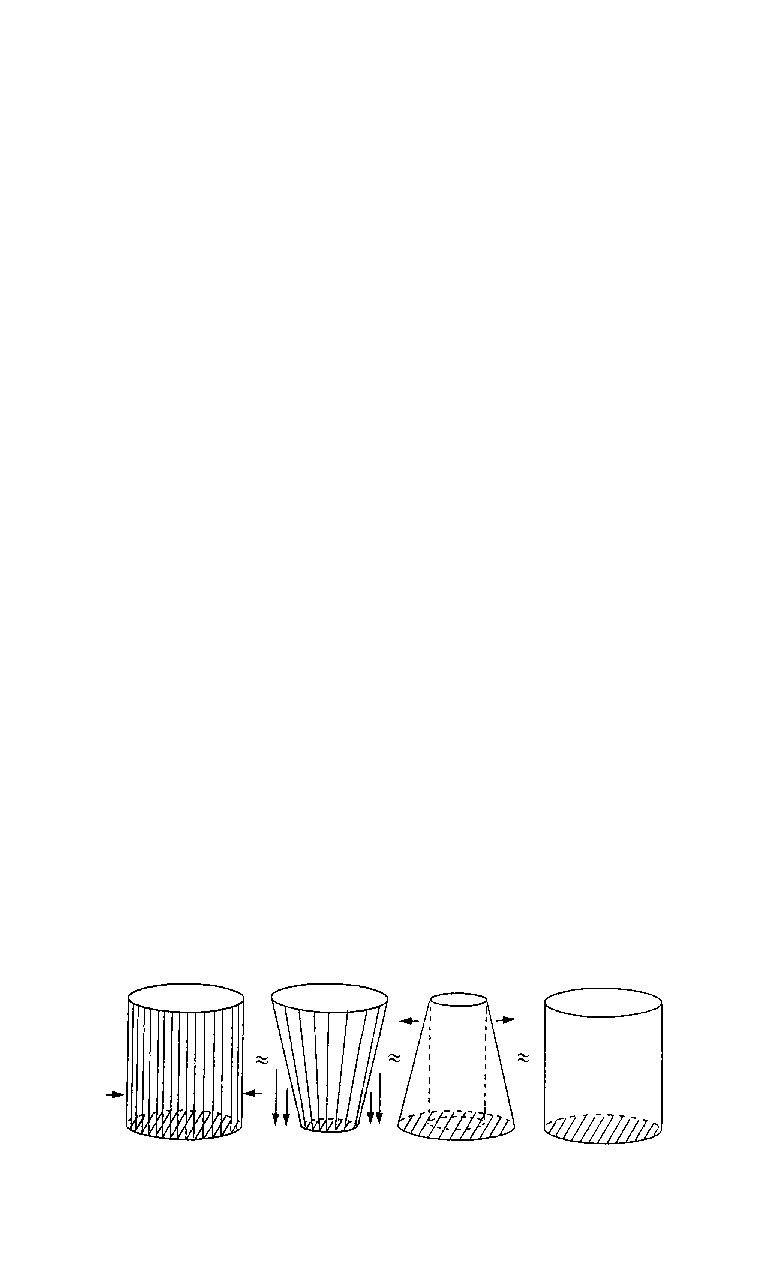
\includegraphics[width=0.5\textwidth]{Images/hom_of_pairs.pdf}
        \caption{Homeomorphism of pairs.}
        \label{fig:homeomorphism of pairs}
    \end{figure}
\end{proof}


The next Theorem shows that a map $E\to B$ that is a Serre fibration locally around each point in $B$ must be a Serre fibration. For Hurewicz fibrations the analogous statement is not generally true, i.e.~a local Hurewicz fibration is not always a Hurewicz fibration, but holds, for example, over paracompact base spaces.

\begin{thm}[{{\cite[Theorem~6.3.3]{tomDieck}}}]\label{thm local fibration}
    Let $p:E\to B$ be a continuous map and $\mathcal{U}$ a collection of subsets whose interiors cover $B$. If for every $U\in\mathcal{U}$ the restriction $p_U:p^{-1}(U)\to U$ is a Serre fibration, then so is $p$.
\end{thm}
\begin{proof}
    Subdivide the cube $I^n$ into cubes of size $\delta$ and enumerate them $I_i$. We can choose $\delta$ so that each cube $I_i\times I$ is mapped inside a $U\in\mathcal{U}$ by the map $H$ that we seek to lift. This is possible by the Lebesque Lemma~\ref{Lebesque lemma}. Let $V^k\subset I^n$ denote the union of the $k$-dimensional faces of the subdivision of $I^n$.

    We have to solve the lifting problem for the space $I^n$ with initial condition $h_0$. We begin by extending $h_0$ over $I^n\times [0,\delta]$ to a lifting of $H$. We solve the lifting problems 
     \[
    \begin{tikzcd}[every matrix/.append style={name=m}]
       I^n\times\{0\} \cup V^{k-1}\times [0,\delta] \arrow[d,"i",swap]\arrow[r,"\wt{H}(k-1)"]& E\arrow[d,"p"]\\
       I^{n}\times \{0\}\cup V^k\times [0,\delta]\arrow[r,"H",swap]\arrow[ur,"\wt{H}(k)",dashed,swap] & B
    \end{tikzcd}
    \]
    for $k=0,\ldots,n$ with $V^{-1}=\varnothing$ and $\wt{H}(-1)=a$ by induction in $k$. Let $W$ be a $k$-dimensional cube and $\partial W$ the union of its $(k-1)$-dimensional faces. We can solve the lifting problems
     \[
    \begin{tikzcd}[every matrix/.append style={name=m}]
       W\times\{0\} \cup \partial W\times [0,\delta] \arrow[d,"i",swap]\arrow[r,"\wt{H}(k-1)"]& p^{-1}(U)\arrow[d,"p_U"]\\
       W\times [0,\delta]\arrow[r,"H",swap]\arrow[ur,"\wt{H}_W",dashed,swap] & U
    \end{tikzcd}
    \]
    by a map $\wt{H}_W$, since $p_U$ is a Serre fibration; here $U\in\mathcal{U}$ was chosen such that $H(W\times [0,\delta])\subset U$.

    The $\wt{H}_W$'s for different $U\in\mathcal{U}$ combine to a continuous map $\wt{H}(k):V^l\times [0,\delta]\to E$ which covers $H$ and extends $\wt{H}(k-1)$. We define $\wt{H}$ on the first layer $I^n\times [0,\delta]$ as $\wt{H}(n)$. We now treat $I^n\times [\delta,2\delta]$ similarly with initial condition given by $\restr{\wt{H}(n)}{I^n\times\{\delta\}}$ and continue in this manner inductively.
\end{proof}

\begin{prop}[{{\cite[Prop.~3.2.3]{RS2}}}]\label{prop 3.2.3 RS2}
    Serre fibrations have the \textit{lifting property} (without homotopy) with respect to all pairs of the form
    \begin{enumerate}
        \item $(K\times I,(K\times \{0\})\cup(L\times I))$, where $K$ is a $CW$-complex and $L$ is a subcomplex. This constitutes a relative \gls{hlp} for the pair $(K,L)$.
        \item $(K,L)$ where $K$ is a $CW$-complex and $L$ is a subcomplex which is a strong deformation retract of $K$.
    \end{enumerate}
\end{prop}
\begin{proof}
    Let $\pi:E\to B$ be a Serre fibration, let $K$ be a $CW$-complex and $L$ a subcomplex of $K$.

    1. Consider the lifting problem defined by some $f:K\times I\to B$ and an initial conditon $\wt{f}_0:(K\times\{0\})\cup(L\times I)\to E$. We prove the assertion by induction on the dimension $k$ of the cells attached to $L$ to build $K$. The case $k=0$ is trivial. Thus, assume we have already constructed a lifting $\wt f$ over the subspace $(K^{(k)}\cup L)\times I\subset K\times I$ for some $k\geq 0$ and consider a $(k+1)$-cell $C$ not contained in $L$ with characteristic map $\chi:\bbD^{k+1}\to K$. Since $C$ is not contained in $L$, we have $C\cap (K^{(k)}\cup L)=C\cap L^{(k)}$. Hence, we wish to extend $\wt{f}$ from 
    \[(C\times\{0\}) \cup((C\cap K^{(k)})\times I)\subset C\times I\]
    to a lifting of $f$ on $C\times I$. Assume that we can extend
    \[\wt{f}\circ \restr{(\chi\times\id_I)}{(\bbD^{k+1}\times\{0\})\cup (\partial \bbD^{k+1}\times I)}\]
    to a lifting of $f\circ (\chi\times\id_I)$ on $\bbD^{k+1}\times I$. Since $\chi $ is injective on $\Int \bbD^{k+1}$, this lifting uniquely determines a lift of $f$ on $C\times I$. By Proposition~\ref{prop 3.1.11 RS2}, applied to the $CW$-complex $C\times I$, the latter is continuous.

    This argument shows that in order to prove that $\wt f$ extends to a lifting of $f$ over $(K^{(k+1)}\cup L)\times I$, it suffices to show that $\pi$ has the relative \gls{hlp} with respect to the pair $(\bbD^{k+1},\bbS^k)$. This holds by Proposition~\ref{prop 3.2.4 tomDieck} since $\pi$ is Serre fibration.

    2. Let $F:K\times I\to K$ be a strong deformation retraction from $K$ to $L$ and consider the lifting problem defined by some $f:K\to X$ and an appropriate initial condition $\wt{f}_0:L\to E$. Define $g:K\times I\to B$ by $g=f\circ F$. Since $F$ maps subsets $K\times\{1\}$ and $L\times I$ to $L$, we can also define
    \[\wt{g}_0:(K\times\{1\})\cup(L\times I)\to E,\quad \wt{g}_0(x,t)=\wt{f}_0(F(x,t)).\]
    A brief calculation shows that $\wt{g}_0$ is a lifting of $g$ over the subset $(K\times\{1\})\cup(L\times I)$. Hence, according to point 1, it can be extended to a lift $\wt{g}$ of $g$. Then, another brief calculation shows that the mapping $\wt f:K\to E$ defined by $\wt{f}(x)=\wt{g}(x,0)$ is a lifting of $f$ through $\pi$ extending $\wt{f}_0$.
\end{proof}

\begin{thm}\label{thm 6.3.1 tomDieck}
    Let $p:E\to B$ be a Serre fibration. For $B_0\subset B$ let $E_0=p^{-1}(B_0)$. Choose basepoints $*\in B_0$ and $* \in p^{-1}(*)$. Then $p$ induces for $n\geq 1$ a bijection $p_\ast:\pi_n(E,E_0,*)\to \pi_n(B,B_0,*)$.
\end{thm}
\begin{proof}
    First we show surjectivity. Let $g \in \pi_n(B,B_0,*)$ be represented by $\gamma:(\bbD^n,\bbS^{n-1},*)\to (B,B_0,*)$.
    By \gls{hlp} there exists a lifting $\wt\gamma:\bbD^n\to E$ with $\wt\gamma(*)=*$ and $p\circ \wt\gamma=\gamma$. We then have $\wt\gamma(\bbS^{n-1})\subset E_0$ and thus $\wt\gamma$ represents a pre-image pf $g$ under $p_\ast$.

    To show injectivity, let $g_0,g_1\in \pi_n(E,E_0,*)$ be represented by $\gamma_0,\gamma_1$ and have the same image under $p_\ast$. Then there exists a homotopy $\phi_t:(\bbD^n,\bbS^{n-1},*)\to (B,B_0,*)$ such that $\phi_0=p\circ \gamma_0$ and $\phi_1=p\circ \gamma_1$. Consider the subspace $T=\bbD^n\times\partial I\cup *\times I$ and define $G:T\to E$ by 
    \[G(x,t)=
        \begin{cases}
            \phi_t(x),& x\in \bbD^n, t\in\{0,1\},\\
            *, & x=*, t\in I.
        \end{cases}
    \]
    The set $T\subset \partial(\bbD^n\times I)$ is transformed into $*$ if one interchanges the last two coordinates. By \gls{hlp} again, there exists a map $H:\bbD^n\times I\to E$ such that $\restr{H}{T}=G$ and $p\circ H=\phi$. We can view $H$ as a homotopy from $\gamma_0$ to $\gamma_1$.
\end{proof}
By taking $B_0$ to be a single point, we get the following corollary, which for $n\geq 2$ is just a generalization of Corollary~\ref{cor homotopy groups of coverings} for covering spaces to all fibrations.
\begin{cor}
    Given a Serre fibration $p:E\to B$ with $F=p^{-1}(*)$, there is an isomorphism of homotopy groups
    \[\pi_n(E,F,*)\cong \pi_n(B,*),\quad n\geq 1.\]
\end{cor}
With the help of this isomorphism, we immediately get a special case of the long exact sequence of a pair (Theorem~\ref{thm long exact seq of homotopy}).
\begin{thm}[Exact sequence of a Serre fibration]
    For a Serre fibration $p:E\to B$ with inclusion $i:F=p^{-1}(b)\subset E$ and $e\in F$ the sequence
    \begin{multline}
        \cdots \to \pi_n(F,e)\overset{i_\ast}{\to}\pi_n(E,e)\overset{p_\ast}{\to}\pi_n(B,b)\overset{\partial}{\to}\pi_{n-1}(F,e)\to\cdots\\ 
        \to \pi_0(E,e)\to \pi_0(B,b)
    \end{multline}
    is exact.
\end{thm}

The boundary map $\partial$ has the following description. Let $f:(I^n,\partial I^n)\to (B,b)$ be given. View $f$ as a map $I^{n-1}\times I\to B$ and lift it to $\wt{f}:I^n\to E$, constant and equal to $e$ on $J^{n-1}=I^{n-1}\times \{0\}\cup \partial I^{n-1}\times I$. Then $\partial[f]$ is represented by $\restr{\wt{f}}{I^{n-1}\times \{1\}}$. In plain language, a ``loop'' representing an element of $\pi_n(B)$ in the base can be lifted to a ``path'' in the total space whose ``endpoints'' lie in the same fiber $F$, and by restricting to $F$ we get a lower-dimensional ``loop'' that represents an element of $\pi_{n-1}(F)$. The very end of the sequence requires a little extra work.

\begin{defn}[Trivialization]
    Let $\pi :E\to B$ be continuous and $U\subset B$ open and contained in the image of $\pi$. A \emph{trivialization} of $\pi$ over $U$ is a homeomorphism $\varphi:\pi^{-1}(U)\to U\times F$ over $U$, i.e.\ a homeomorphism which satisfies $\mathrm{pr}_1\circ \varphi=\pi$ (where $\mathrm{pr}_1$ is the natural projection onto the first component of the direct product). This condition determines $F$ up to a homeomorphism since $\varphi$ induces a homeomorphism of $\pi^{-1}(u)$ with $\{u\}\times F$.
\end{defn}

\begin{defn}[Locally trivial map]
    The map $\pi$ is \emph{locally trivial} if there exists an open covering $\mathcal{U}$ of $B$ such that $\pi$ has a trivialization over each $U_\alpha\in \mathcal{U}$. 
\end{defn}

Note that a locally trivial map is open and hence a topological quotient map.

\begin{example}
    Since a product projection is a fibration, we have by Theorem~\ref{thm local fibration} that any locally trivial map is a Serre fibration.
\end{example}
\begin{example}[Exact sequence of a covering space]
    Let $p:E\to B$ be a covering map with typical fiber $F$. Since each map $\bbD^n\to F$ must be constant because of discreteness of $F$, $\pi_n(F,*)$ is trivial for $n\geq 1$. The exact sequence of $p$ then confirms the isomorphisms $\pi_n(E,f)\cong \pi_n(B,b)$, $n\geq 2$, that we proved in Corollary~\ref{cor homotopy groups of coverings}. Moreover we have the exact sequence (omitting the common basepoint)
    \[1\to \pi_1(E)\overset{p_\ast}{\to} \pi_1(B)\overset{\partial}{\to} \pi_0(F)\overset{i_\ast}{\to} \pi_0(E)\overset{p_\ast}{\to} \pi_0(B)\to 1\]
    with the inclusion $i:F=p^{-1}(*)\subset E$ and $\pi_0(F)=F$. It yields for the universal covering $p:\bbR \to \bbS^1$ the familiar bijection $\partial:\pi_1(\bbS^1)\cong \bbZ$.
\end{example}

\begin{defn}[Hopf fibrations]\label{def: Hopf fibrations}
    Looking slightly ahead, consider $\bbS^{2n-1}\subset \bbC^n$ as a space with a free action of $\bbS^1=U(1)$ induced from scalar multiplication by $\rme^{2\pi\rmi  t}$. Let $U_j$ be the set of points $z=(z_1,\ldots,z_n)\in\bbC^n$ with $z_j\neq 0$. The map $z\mapsto z_j/|z_j|$ shows that $U_j\cong \bbR^{2n-1}\times \bbS^1$ is a trivial $U(1)$-space. The orbit space of this action is exactly $\mathbb{C}P^{n-1}=\bbS^{2n-1}\slash \bbS^1$. The Hopf fibration is defined as the orbit map $p:\bbS^{2n-1}\to \mathbb{C}P^{n-1}$. It is indeed a fibration because it is clearly trivial over $U_j\cap \bbS^{2n-1}$. We will also see a more explicit definition of the most important $n=2$ Hopf fibration later on.
\end{defn}

\begin{example}
    The exact sequence for the Hopf fibration, combined with $\pi_i(\bbS^1)=0$ for $i>1$ (see Corollary~\ref{cor: homotopy groups of circle}), yields the isomorphisms
    \[p_\ast: \pi_i(\bbS^{2n+1})\cong \pi_i(\mathbb{C}P^n),\; i\geq 3;\]
    and in particular $\pi_i(\bbS^3)\cong \pi_i(\bbS^2)$ for $i\geq 3$, since $\mathbb{C}P^1\cong \bbS^2$.
\end{example}

\begin{prop}[{{\cite[Prop.~6.3.8]{tomDieck}}}]\label{prop 6.3.8 tomDieck}
    Let $p:(E_1,E_0)\to B$ be a relative Serre fibration, i.e.\ $p:E_1\to B$ is a Serre fibration and the restriction $\restr{p}{E_0}$ is also a Serre fibration. Let $(F^1_b,F^0_b)$ be the pair of fibers over $p_1(e)=b\in B$. Then:
    \begin{enumerate}
        \item The inclusion induces bijections $\pi_n(F_b^1,F_b^0,e)\cong\pi_n(E_1,E_0,e)$.
        \item $\pi_0(E_0)\to \pi_0(E_1)$ is surjective iff $\pi_0(F_b^0)\to \pi_0(F_b^1)$ is surjective for each $b\in B$.
    \end{enumerate}
\end{prop}
\begin{proof}
    (1) We first prove the claim for $n=1$ and begin with surjectivity. Let $f:(I,\partial I,0)\to (E_1,E_0,e)$ be given. The path $\widebar{p\circ f}:I\to B$ (recall that the bar represents reversing the path) is lifted to $g:I\to E_0$ with initial point $f(1)$. Then $g(1)\in F^0_b$, and $f$ and $f\bullet g$ represent the same element in $\pi_1(E_1,E_0,e)$. The projection $p\circ(f\bullet g)$ is a nullhomotopic loop with basepoint $b$. We lift a nullhomotopy to $E_1$ with initial condition $f\bullet g$ on $I\times\{0\}$ and constant on $\partial I\times I$. The lifting is a homotopy $(I,\partial I,0)\times I\to (E_1,E_0,e)$ from $f\bullet g$ to a map into $(F^1_b,F^0_b,e)$. This proves the surjectivity.

    Suppose $f_0,f_1:(I,\partial I,0)\to (F^1_b,F^0_b,e)$ are given, and let $K:(I,\partial I,0)\times I\to (E_1,E_0,e)$ be a homotopy from $f_0$ to $f_1$. We lift $\widebar{p\circ K}$ to $L:I^2\to E_0$ with initial condition $L(s,0)=K(s,1)$ and $L(0,t)=L(1,t)=e$. The homotopy $p\circ(K\bullet_2 L)$ is a homotopy of loops which is $\rel \partial I^2$ homotopic to the constant map. We lift a homotopy to $E_1$ with initial condition $K\bullet_2 L$ on $I^2\times\{0\}$ and constant on $\partial I^2\times I$. The end is a homotopy from $f_0\bullet \kappa_e$ to $f_1\bullet\kappa_e$ (where $\kappa_e$ is a constant loop at $e$). This proves the injectivity.

    The higher dimensional case is obtained by an application to the relative Serre fibration $(\Omega^n F^1_b,\Omega^n F^0_b)\to (\Omega^n E_1,\Omega^nE_0)\to B$.

    (2) Suppose $\pi_0(E)\to \pi_0(E_1)$ is surjective. The argument above for surjectivity is used to show the surjectivity of $\pi_0(F^0_b)
    to \pi_0(F^1_b)$. The opposite implication is easy.
\end{proof}





\subsection{Higher connectivity}

For many applications it is important to know that the homotopy groups of a space vanish in a certain range. We discuss several reformulations of this fact. In the following $\pi_0(X,x_0)=\pi_0(X)$. The space $\bbD^0$ is a singleton and $\bbS^{-1}=\varnothing$.

\begin{prop}[{{\cite[Prop.~6.7.1]{tomDieck}}}]\label{prop 6.7.1 tomDieck} 
Let $n\geq 0$. \gls{tfae}:
\begin{enumerate}
    \item $\pi_n(X,x)=0$ for each $x\in X$.
    \item Each map $\bbS^n\to X$ has an extension to $\bbD^{n+1}$.
    \item Each map $\partial \bbD^{n+1}\to X$ has an extension to $\bbD^{n+1}$.
\end{enumerate}
\end{prop}
\begin{proof}
    The case $n=0$ is trivial. The equivalence of (2) and (3) is a consequence of the homeomorphism $(\bbD^{n+1},\bbS^n)\cong(I^{n+1},\partial I^{n+1})$. Suppose $f:\bbS^n\to X$ is given. Use $e_1=(1,0,\ldots)\in \bbS^n$ as a base point and think of $f$ as representing an element of $\pi_n(X,x)$. If (1) holds, then $f$ is pointed null homotopic. A null homotopy $\bbS^n\times I\to X$ factors over the quotient map $\bbS^n\times I\to \bbD^{n+1}$, $(x,t)\mapsto (1-t)e_1+tx$ and yields an extension of $f$. Conversely, let an element $\alpha$ of $\pi_n(X,x)$ be represented by a pointed map $f:(\bbS^n,e_1)\to (X,x)$. If this map has an extension $F$ to $\bbD^{n+1}$, then $(F,f)$ represents $\beta\in \pi_n(X,X,x)=0$ with $\partial\beta=\alpha$.
\end{proof}

\begin{prop}[{{\cite[Prop.~6.7.3]{tomDieck}}}]\label{prop 6.7.3 tomDieck}
    Let $n\geq 1$. The following assertions about a topological pair $(X,A)$ are equivalent:
    \begin{enumerate}
        \item $\pi_n(X,A,*)=0$ for each choice of $*\in A$.
        \item Each map $f:(I^n,\partial I^n)\to (X,A)$ is as a map of pairs homotopic to a constant map.
        \item Each map $f:(I^n,\partial I^n)\to (X,A)$ is homotopic $\rel \partial I^n$ to a map into $A$.
    \end{enumerate}
\end{prop}
\begin{proof}
    $(1)\Rightarrow(2)$. Let $f:(I^n,\partial I^n)\to (X,A)$ be given. Since $J^{n-1}$ is contractible, there exists a homotopy of the restriction $f:J^{n-1}\to A$ to a constant map. Since $J^{n-1}\subset \partial I^n$ and $\partial I^n\subset I^n$ are cofibrations, $f$ is as a map of pairs homotopic to $g:(I^n,\partial I^n)\to (X,A)$ such that $g(J^{n-1})=\{a_0\}$. Since $\pi_n(X,A,a_0)=0$, the map $g:(I^n,\partial I^n,J^{n-1})\to (X,A,a_0)$ is nullhomotopic as a map of triples.

    $(2)\Rightarrow(3)$ by the compression criterion (Proposition~\ref{prop: compression criterion}).

    $(3)\Rightarrow (1)$. Let $f:(I^n,\partial I^n,J^{n-1})\to (X,A,*)$ be given. By assumption (3), $[f]$ is contained in the image of $\pi_n(A,A,*)\to \pi_n(X,A,*)$. Now use $\pi_n(A,A,*)=0$.
\end{proof}



\begin{defn}[$n$-compressible pair]\index{$n$-compressible space}
    A topological pair $(X,A)$ is called $n$-compressible if (1)-(3) in Proposition~\ref{prop 6.7.3 tomDieck} hold. More generally, we call a map $f:X\to Y$ $n$-compressible if for each commutative diagram 
    \[
    \begin{tikzcd}[every matrix/.append style={name=m}, row sep=large, column sep=large]
       \partial \bbS^{n-1} \arrow[r,"\varphi"]\arrow[d,"i",swap] & X\arrow[d,"f"]\\
       \bbD^n \arrow[r,"\Phi", swap]\arrow[ur,"\Psi",dashed,swap] & Y
    \end{tikzcd}
    \]
    there exists $\Psi:\bbD^n\to X$ such that $\restr{\Psi}{\partial \bbD^n}=\varphi$ and $f\circ \Psi\simeq \Phi$ $\rel \partial \bbD^n$ (this amounts to (3) of Proposition~\ref{prop 6.7.3 tomDieck}). This notion is invariant under compositions with homotopy equivalences of the target space $Y$.
\end{defn}

\begin{prop}[{{\cite[Prop.~6.7.5]{tomDieck}}}]\label{prop 6.7.5 tomDieck}
    Let $n\geq 0$. The following assertions about a pair $(X,A)$ are equivalent:
    \begin{enumerate}
        \item Each map $f:(\bbD^q,\partial \bbD^q)\to (X,A)$, $q\in (0,\ldots,n)$ is $\rel \partial \bbD^q$ homotopic to a map into $A$.
        \item The inclusion $j:A\hookrightarrow X$ induces for each basepoint $a\in A$ a bijection $j_\ast:\pi_q(A,a)\to \pi_q(X,a)$ for $q<n$ and a surjection for $q=n$.
        \item $\pi_q(X,A,a)=0$ for $q=1,\ldots,n$ and each $a\in A$, and $\pi_0(A)\to \pi_0(X)$ is surjective.
    \end{enumerate}
\end{prop}
\begin{proof}
    $(1)\Leftrightarrow (3)$. The surjectivity of $\pi_0(A)\to \pi_0(X)$ is equivalent to (1) for $q=0$. The other cases follow from Proposition~\ref{prop 6.7.3 tomDieck}.

    $(2)\Leftrightarrow(3)$ follows from the exact sequence of the pair (Theorem~\ref{thm long exact seq of homotopy}).
\end{proof}


\begin{defn}[$n$-connected pair]\index{$n$-connected pair}
    A topological pair $(X,A)$ is called $n$-connected if (1)-(3) in Proposition~\ref{prop 6.7.5 tomDieck} hold. We call $(X,A)$ $\infty$-connected if the pair is $n$-connected for each $n$. A pair is $\infty$-connected iff $j_\ast:\pi_n(A,a)\to \pi_n(X,a)$ is always bijective. If $X\neq\varnothing$ but $A=\varnothing$ we say that $(X,A)$ is $(-1)$-connected, and $(\varnothing,\varnothing)$ is $\infty$-connected.
\end{defn}

\begin{defn}[Cone]\index{Cone}
    Given a space $X$, its cone $CX$ is defined as result of attaching the cylinder $X\times [0,1]$ by its face $X\times\{0\}$ to a point $*$ along the projection $p:X\times \{0\}\to *$.
\end{defn}


\begin{prop}[{{\cite[Prop.~6.7.6]{tomDieck}}}]\label{prop 6.7.6 tomDieck}
    Let $n\geq 0$. The following assertions about a space $X$ are equivalent:
    \begin{enumerate}
        \item $\pi_q(X,x)=0$ for $0\leq q\leq n$ and $x\in X$.
        \item The pair $(CX,X)$ is $(n+1)$-connected.
        \item Each map $f:\partial I^q\to X$, $0\leq q\leq n+1$ has an extension to $I^q$.
    \end{enumerate}
\end{prop}
\begin{proof}
    The cone $CX$ is contractible, therefore $\partial:\pi_{q+1}(CX,X,*)\cong \pi_q(X,*)$. This and Proposition~\ref{prop 6.7.5 tomDieck} shows the equivalence of (1) and (2). The equivalence of (1) and (3) is based on Proposition~\ref{prop 6.7.1 tomDieck}.
\end{proof}

\begin{defn}[$n$-connected space]\index{$n$-connected space}
    A space $X$ is called $n$-connected if (1)-(3) in Proposition~\ref{prop 6.7.6 tomDieck} hold. Note that this is compatible with previous definitions for $n=0$ (path-connected) and $n=1$ (simply-connected).
\end{defn}

\begin{defn}[$n$-equivalence]\index{$n$-equivalence}\index{Weak equivalence}
    Let $f:X\to Y$ be a map and $X\subset Z_f$ the inclusion into the mapping cylinder (recall the definition in Figure~\ref{fig:mapping cyl}). Then $f$ is said to be $n$-connected if $(Z_f,X)$ is $n$-connected. We then also say that $f$ is an $n$-equivalence. Thus $f$ is $n$-connected iff $f_\ast:\pi_q(X,x)\to \pi_q(Y,f(x))$ is for each $x\in X$ bijective for $q<n$ and surjective for $q=n$. If $f$ is an $\infty$-equivalence we also call it a weak (homotopy) equivalence, which happens iff $f_\ast$ is bijective for all $x\in X$ in all degrees.
\end{defn}

\begin{prop}[{{\cite[Prop.~6.7.7]{tomDieck}}}]\label{prop 6.7.7 tomDieck}
    Let $p:(E_1,E_0)\to B$ be a relative Serre fibration (see Proposition~\ref{prop 6.3.8 tomDieck}). Let $(F^1_b,F^0_b)$ be the pair of fibers over $b\in B$. Then the pair $(E_1,E_0)$ is $n$-connected iff the pairs $(F^1_b,F^0_b)$ are $n$-connected for all $b\in B$.
\end{prop}
\begin{proof}
    This is a direct consequence of Proposition~\ref{prop 6.3.8 tomDieck}.
\end{proof}

\begin{thm}[{{\cite[Theorem~6.7.9]{tomDieck}}}]\label{thm 6.7.9 tomDieck}
    Let $\varphi:(X,X_0,X_1)\to (Y,Y_0,Y_1)$ be a map such that the restrictions $\varphi_i:X_i\to Y_i$ are $n$-connected and $\varphi_{01}:X_0\cap X_1\to Y_0\cap Y_1$ is $(n-1)$-connected. Suppose $X=X_0^\circ \cup X_1^\circ$ and $Y=Y_0^\circ \cup Y_1^\circ$ where $\ ^\circ$ denotes interiors. Then $\varphi $ is an $n$-equivalence.
\end{thm}

\begin{cor}[{{\cite[Prop.~6.7.10]{tomDieck}}}]\label{prop 6.7.10 tomDieck}
    Let $f:X\to Y$ be an $n$-connected map between spaces with nondegenerate basepoints. Then the suspension $\Sigma f:\Sigma X\to \Sigma Y$ is $(n+1)$-connected. If $X$ is $n$-connected, then $\Sigma X$ is $(n+1)$-connected. The sphere $\bbS^{k+1}$ is $k$-connected.
\end{cor}
\begin{proof}
    Let $\Sigma 'X$ denote the unpointed suspension of $X$. This is a quotient of $X\times I$ and covered by the open cones $C_0=X\times [0,1)\slash X\times\{0\}$ and $C_1=X\times (0,1]\slash X\times\{1\}$ with intersection $X\times (0,1)$. We can apply Proposition~\ref{prop 6.7.7 tomDieck} directly; the cones are contractible and therefore the induced maps $C_j(X)\to C_j(Y)$ are $\infty$-connected. In the case of a space $X$ with a nondegenerate basepoint the quotient map $\Sigma 'X\to \Sigma X$ is a homotopy equivalence.
\end{proof}

\begin{thm}[{{\cite[Theorem~6.7.11]{tomDieck}}}]\label{thm 6.7.11 tomDieck}
    Let $f:X\to Y$ be a continuous map. Let $\{U_j\}_j$ and $\{V_j\}_j$ be open coverings of $X$ and $Y$ such that $f(U_j)\subset V_j$. Suppose that for each finite subset of indices the induced map $f_J:\bigcap_{j\in J}U_j\to \bigcap_{j\in J}V_j$ is a weak equivalence. Then $f$ is a weak equivalence.
\end{thm}
\begin{proof}
    By passage to the mapping cylinder we can assume that $f$ is an inclusion. Let $h:(I^n,\partial I^n)\to (Y,X)$ be given. We have to deform $h$ $\rel \partial I^n$ into $X$. By compactness of $I^n$ is suffices to work with finite coverings. A simple induction reduces the problem to a covering by only two sets $j=0,1$. Then we apply Theorem~\ref{thm 6.7.9 tomDieck}.
\end{proof}






\subsection{Excision for homotopy groups}

\begin{thm}[Blakers-Massey excision theorem]
    Let $X=U_0\cup U_1$ be covered by two open subspaces $U_0$ and $Y_1$ with non-empty intersection $V=U_0\cap U_1$. Suppose that $(U_0,V)$ is $p$-connected and $(U_1,V)$ is $q$-connected, i.e.
    \[
    \begin{matrix}
        \pi_i(U_0,V,*)=0,\quad 1\leq i\leq p,\; p\geq 0,\\
        \pi_i(U_1,V,*)=0,\quad 1\leq i\leq q,\; q\geq 0
    \end{matrix}
    \]
    for each basepoint $*\in V$. Then the \emph{excision map}, induced by the inclusion,
    \[i_\ast : \pi_n(U_1,V,*)\to \pi_n(X,U_0,*)\]
    is an isomorphism for $1\leq n <p+q$ and surjective for $n=p+q$ (for each $*\in X)$. In the case $p=0$, there is no condition on $\pi_i(U_0,V,*)$.
\end{thm}

\begin{cor}[{{\cite[Prop.~6.4.2]{tomDieck}}}]\label{prop 6.4.2 tomDieck}
    If in the above $(U_1,V)$ is $q$-connected then $(X,U_0)$ is $q$-connected.
\end{cor}
\begin{proof}
    This is a special case of the excision theorem which also directly follows from Theorem~\ref{thm 6.7.9 tomDieck}.
\end{proof}

For the sphere $\bbS^n$, introduce the following hemispheres and punctured spheres
\[\bbD^n_\pm=\{x\in \bbS^n\subset \bbR^{n+1}\mid \pm x_{n+1}\geq 0\}\subset H^n_\pm=\{x\in \bbS^n\mid x\neq \pm e_{n+1}\}.\]
We use the equatorial point $*=-e_1$ as a basepoint.

\begin{lem}[{{\cite[Lemma~6.4.3]{tomDieck}}}]\label{lem 6.4.3 tomDieck}
   There are isomorphisms $\partial:\pi_{i+1}(D_-^{n+1},\bbS^n,*)\to \pi_i(\bbS^n,*)$ for $i\geq 0$, $n\geq 0$ and $\pi_i(\bbS^n,*)\to \pi_i(\bbS^n,D_\pm^n,*)$ for $i\geq 0$, $n\geq 1$.
\end{lem}
\begin{proof}
    In the first case we use the exact sequence of the pair $(\bbD^{n+1}_-,\bbS^n)$. The space $\bbD^{n+1}_-$ is contractible and hence $\pi_i(\bbD^{n+1}_-,*)=0$ for $i\geq 0$ and $n\geq 0$.

    In the second case we consider similarly the exact sequence of $(\bbS^n,\bbD^n_\pm)$. Note that $*=-e_1\in D_\pm^n$ for $n\geq 1$.
\end{proof}

Thus for $n\geq 0$ we have a diagram with the isomorphisms 
\[
    \begin{tikzcd}[every matrix/.append style={name=m}, row sep=large, column sep=large]
       \pi_i(\bbS^n,*) \arrow[r,"E"] & \pi_{i+1}(\bbS^{n+1},*)\arrow[d,"\cong"]\\
       \pi_{i+1}(\bbD^{n+1}_-,\bbS^n,*)\arrow[u,"\overset{\partial}{\cong}",swap] \arrow[r,"i_\ast", swap] & \pi_{i+1}(\bbS^{n+1},D_+^{n+1},*).
    \end{tikzcd}\label{3795}
\]
The morphism $i_\ast$ is induced by the inclusion and $E$ is defined so as to make the diagram commutative. Note that the inductive proof of (1) in the next Theorem uses only Corollary~\ref{prop 6.4.2 tomDieck}.

\begin{thm}[{{\cite[Thm~6.4.4]{tomDieck}}}]\label{thm 6.4.4 tomDieck}
    \begin{enumerate}
        \item $\pi_i(\bbS^n)=0$ for $i<n$ (recall that we already showed this in Corollary~\ref{cor pi_n(S^k)=0}).
        \item The homomorphism $i_\ast$ in diagram (\ref{3795}) is an isomorphism for $i\leq 2n-2$ and an epimorphism for $i=2n-1$. A similar statement holds for $E$.
    \end{enumerate}
\end{thm}
\begin{proof}
    Let $N(n)$ be the statement (1) and $E(n)$ be the statement (2). Obviously $N(1)$ holds. Assume $N(n)$ holds. We then deduce $E(n)$. We apply the excision theorem to $(X,U_0,U_1,V)=(\bbS^{n+1},D_+^{n+1},D_-^{n+1},\bbS^n)$. By $N(n)$ and Lemma~\ref{lem 6.4.3 tomDieck} we have $\pi_i(\bbS^n)\cong \pi_{i+1}(D_\pm^{n+1},\bbS^n)=0$ for $0\leq i <n$. We use the excision theorem for $p=q=n$ and see that $i_\ast$ is surjective for $i+1\leq 2n$ and bijective for $i+1\leq 2n-1$. Finally, $E(n)$ and $N(n)$ imply $N(n+1)$.

    In order to have the correct hypotheses for the excision theorem, we thicken the spaces, replace $D_\pm^n$ by $H^n_\pm$ and note that the inclusions $D_\pm^n\subset H^n_\pm$ and $\bbS^{n-1}\subset H^n_+\cap H^n_-$ are homotopy equivalences.
\end{proof}
\begin{cor}[{{\cite[Prop.~5.11]{Bredon}}}] 
    The pair $(\bbD^{n+1},\bbS^n)$ is $n$-connected.
\end{cor}
\begin{proof}
    This follows from the exact sequence $\pi_r(\bbD^{n+1})\to \pi_r(\bbD^{n+1},\bbS^n)\to \pi_{r-1}(\bbS^n)$ for $r\leq n$, where the two groups on the sides vanish.
\end{proof}


\begin{prop}[{{\cite[Prop.~6.4.5]{tomDieck}}}]\label{prop 6.4.5 tomDieck}
    The homomorphism $\pi_i(\bbD^{n+1},\bbS^n,*)\to \pi_i(\bbD^{n+1}\slash \bbS^n,*)$ induced by the quotient map is an isomorphism for $i\leq 2n-1$ and an epimorphism for $i=2n$.
\end{prop}
\begin{proof}
    Consider the commutative diagram
    \[
    \begin{tikzcd}[every matrix/.append style={name=m}, row sep=large, column sep=large]
       \pi_i(D_-^{n+1},\bbS^n,*) \arrow[r]\arrow[d,"i_\ast",swap] & \pi_i(D_-^{n+1}\slash \bbS^n,*) \arrow[d,"(1)"]\\
       \pi_{i+1}(\bbS^{n+1},\bbD^{n+1}_+,*)\arrow[r,"(2)",swap] & \pi_{i}(\bbS^{n+1}\slash D_+^{n+1},*).
    \end{tikzcd}
    \]
    The map (1) is induced by a homeomorphism and the map (2) by a homotopy equivalence, hence both are isomorphisms. Now apply Theorem~\ref{thm 6.4.4 tomDieck}.
\end{proof}

The homomorphism $E$ is essentially the suspension homomorphism:
\[\Sigma_\ast: \pi_n(X)\underset{\cong}{\overset{\partial}{\leftarrow}}\pi_{n+1}(CX,X)\overset{q_\ast}{\to}\pi_{n+1}(CX\slash X)=\pi_{n+1}(\Sigma X)\]
with the quotient map $q:\bbD^{n+1}\to \bbS^{n+1}=\bbD^{n+1}\slash \bbS^n$. The next result is the famous suspension theorem of Freudenthal.

\begin{thm}[Freudenthal's suspension theorem {{\cite[Theorem~6.4.6]{tomDieck}}}]\label{thm 6.4.6 tomDieck freudenthal}
    The suspension $\Sigma_\ast:\pi_i(\bbS^n)\to \pi_{i+1}(\bbS^{n+1})$ is an isomorphism for $i\leq 2n-2$ and an epimorphism for $i=2n-1$.
\end{thm}
\begin{proof}
    We have to show that $q_\ast:\pi_{i+1}(CX,X)\to \pi_{i+1}(CX\slash X)$ is for $X=\bbS^n$ an isomorphism (epimorphism) in the appropriate range. This follows from Proposition~\ref{prop 6.4.5 tomDieck}; one has to use that  $\bbD^{n+1}_-$ is the (pointed) cone on $\bbS^n$.
\end{proof}

\begin{thm}[{{\cite[Theorem~6.4.7]{tomDieck}}}]\label{thm 6.4.7 tomDieck freudenthal}
    $\pi_n(\bbS^n)\cong \bbZ$ and $\Sigma_\ast:\pi_n(\bbS^n)\to \pi_{n+1}(\bbS^{n+1})$ is an isomorphism ($n\geq 1$). The group $\pi_n(\bbS^n)$ is generated by the identity map of $\bbS^n$.
\end{thm}
\begin{proof}
    From the exact sequence of the Hopf fibration $\pi_2(\bbS^3)\to \pi_2(\bbS^2)\to \pi_1(\bbS^1)\to \pi_1(\bbS^3)$ and $\pi_j(\bbS^3)=0$ for $j=1,2$, we obtain an isomorphism $\partial:\pi_2(\bbS^2)\to \pi_1(\bbS^1)\cong \bbZ$. From Theorem~\ref{thm 6.4.6 tomDieck freudenthal} we obtain a surjection $\Sigma_\ast:\pi_1(\bbS^1)\to \pi_2(\bbS^2)$; this is an isomorphism, since both groups are isomorhic to $\bbZ$. For $n\geq 2$, Theorem~\ref{thm 6.4.6 tomDieck freudenthal} directly gives an isomorphism $\Sigma_\ast$. We know that $\pi_1(\bbS^1)$ is generated by the identity map, and $\Sigma_\ast$ respects the identity.
\end{proof}

This proof clearly extends to two cones over any space $X$, so by using the adjunction $[\Sigma X,Y]\cong[X,\Omega Y]$ we get the more general form of this Theorem.

\begin{thm}[Freudenthal's suspension thereom]\index{Theorem!Freudenthal's suspension}
Let $X$ be an $n$-connected space, i.e.\ $\pi_i(X)=0$ for $0\leq i\leq n$. Then the homomorphism $\pi_k(X)\to \pi_k(\Omega \Sigma X)$ induced by the inclusion $X\hookrightarrow \Omega\Sigma X$ is an isomorphism for $k\leq 2n-2$ and an epimorphism for $k=2n-1$.

Furthermore, since $\pi_{k+1}(\Sigma X)\cong[\bbS^{k+1};\Sigma X]\cong[\bbS^k;\Omega \Sigma X]\cong\pi_k(\Omega \Sigma X)$, for $k\leq 2n-2$ there is an isomorphism $\pi_k(X)\cong \pi_{k+1}(\Sigma X)$.
\end{thm}
\begin{proof}
See \cite[Theorem 6.4.6]{tomDieck}.
\end{proof}

\begin{defn}[Degree on spheres]\index{Degree}
    For a map $f:\bbS^n\to \bbS^n$, its degree $\deg f$ is the integer such that $[f]=[\mathrm{id}_{\bbS^n}]^{\deg f}$ in $\pi_n(\bbS^n)$.
\end{defn}

\begin{example}[Hopf fibrations]\label{example Hopf pi3(S2)}
    We continue the discussion of the Hopf fibrations \ref{def: Hopf fibrations}. The Hopf fibration $\bbS^{2n+1}\to \mathbb{C}P^n$ and $\pi_i(\bbS^{2n+1})=0$ for $i\leq 2n$ yield $\pi_2(\mathbb{C}P^n)\cong \pi_1(\bbS^1)\cong \bbZ$ and $\pi_i(\mathbb{C}P^n)=0$ for $0\leq i \leq 2n$, $i\neq 2$. The inclusion $\bbS^{2n+1}\to \bbS^{2n+3}$, $z\mapsto (z,0)$ induces an embedding $\mathbb{C}P^n\subset \mathbb{C}P^{n+1}$. We compare the corresponding Hopf fibrations and their exact sequences and conclude $\pi_2(\mathbb{C}P^n)\cong \pi_2(\mathbb{C}P^{n+1})$. Let $\mathbb{C}P^\infty =\bigcup_{n\geq 1}\mathbb{C}P^n$ be the colimit (the topology on it is defined as the finest topology under which all inclusions $\mathbb{C}P^n\hookrightarrow \mathbb{C}P^\infty$ are continuous). The inclusions induce $\pi_i(\mathbb{C}P^n)\cong\pi_i(\mathbb{C}P^\infty)$ for $i\leq 2n$. A proof uses the fact that a compact subset of $\mathbb{C}P^\infty$ is contained in some finite $\mathbb{C}P^N$. Therefore $\mathbb{C}P^\infty$ is a space with a single nontrivial homotopy group $\pi_2(\mathbb{C}P^\infty)\cong\bbZ$.

    Particularly notable is the special case 
    \[\pi_3(\bbS^2)\cong \pi_3(\bbS^3)\cong\bbZ.\]
    This is the first of the ``nontrivial'' homotopy groups of spheres $\pi_k(\bbS^n), k>n$, and the only one that can be computed without much more advanced homology theory.

    We have the similar results for real projective spaces. The double coverings $\bbS^n\to \bbR P^n$ are used to show that $\pi_1(\bbR P^2)\cong \pi_1(\bbR P^3)\cong\cdots =\cong \pi_1(\bbR P^\infty)\cong \bbZ_2$, induced by the inclusions $\bbR P^n\hookrightarrow\bbR P^{n+1}$ for $i<n$ and $\pi_i(\bbR P^n)=0$ for $0\leq i< n$, $i\neq 1$. The space $\bbR P^\infty$ therefore has a single nontrivial homotopy group $\pi_1(\bbR P^\infty)\cong\bbZ_2$.
\end{example}


\begin{example}[Lens spaces]\index{Lens spaces}
    Recall the lens space $L=L_m(l_1,\ldots,l_n)$ from Example~\ref{example Lens spaces}. It can be given a structure of a $CW$-complex with one cell in each dimension from $0$ to $2n-1$ so that the degree of the attaching maps alternates between $0$ and $m$ (starting with degree $0$ for the map $\partial \bbD^1\to L^{(0)}$).
\end{example}


\begin{example}[$\pi_3(\bbS^2\vee \bbS^2)\cong \bbZ^3$]
    Let us compute $\pi_3(\bbS^2\vee \bbS^2)$. We have an inclusion $i: \bbS^2\vee \bbS^2\hookrightarrow \bbS^2\times \bbS^2$, because $\bbS^2\times \bbS^2$ can be realized as a $CW$-complex that differs from $\bbS^2\vee \bbS^2$ only by an addition of a 4-cell. Observe that the induced homomorphism on the homotopy groups is surjective:
    \[i_\ast: \quad \pi_n(\bbS^2\vee \bbS^2)\to \pi_n(\bbS^2\times \bbS^2)=\pi_n(\bbS^2)\oplus \pi_n(\bbS^2).\]
    (Here we used the fact that a smash product with $\bbS^k$ is homeomorphic to the iterated reduced suspension $\Sigma^k$, and $\Sigma^k \bbS^n=\cong \bbS^{n+k}$.) This allows us to insert extra zeroes into the long exact sequence for the pair $(\bbS^2\times \bbS^2,\bbS^2\vee \bbS^2)$ without breaking its exactness, which splits it into the short exact sequences
    \[0\to \pi_{n+1}(\bbS^2\times \bbS^2,\bbS^2\vee \bbS^2)\to \pi_n(\bbS^2\vee \bbS^2)\overset{i_\ast}{\to} \pi_n(\bbS^2\times \bbS^2)\to 0.\]
    For $n=3$, since $\bbS^2\vee \bbS^2$ is 1-connected and the remaining 4-cell is 4-connected, we can use the excision theorem to compute
    \[\pi_4(\bbS^2\times \bbS^2,\bbS^2\vee \bbS^2)\cong \pi_4(\bbS^2\times \bbS^2\slash \bbS^2\vee \bbS^2)\cong \pi_4(\bbS^2\wedge \bbS^2) \cong\pi_4(\bbS^4)\cong \bbZ.\]
    At the same time, $\pi_3(\bbS^2\times \bbS^2)=\pi_3(\bbS^2)\oplus \pi_3(\bbS^2)=\bbZ^2$ (generated by the Hopf fibrations from the preceding Example~\ref{example Hopf pi3(S2)}). Thus we have the exact sequence
    \[0\to \bbZ\to \pi_3(\bbS^2\vee \bbS^2)\to \bbZ^2\to 0,\]
    which implies $\pi_3(\bbS^2\vee \bbS^2)=\bbZ^3$ because every short exact sequence of the form $0\to A\overset{i}{\to} B\overset{p}{\to} \bbZ^2\to 0$ splits (the splitting monomorphism $j:\bbZ^2\to B$ can be constructed by defining it on the basis $j(1,0)=b_1$ and $j(0,1)=b_2$, where $b_1,b_2\in B$ are any two elements such that $p(b_1)=(1,0)$ and $p(b_2)=(0,1)$; it is then easy to check that $p\circ j=\id_{\bbZ^2}$ and hence $B\cong A\oplus \bbZ^2$).

    This construction is a special case of the \emph{Whitehead product}\index{Whitehead product} $\pi_k(X)\times\pi_l(X)\to \pi_{k+l-1}(X)$. Given $f:\bbS^k\to X$ and $g:\bbS^l\to X$, their Whitehead product is the homotopy class denoted
    \[[f,g]\in \pi_{k+l-1}(X)\]
    and represented by the composition 
    \[\bbS^{k+l-1}\overset{\chi}{\to} \bbS^k\vee \bbS^l\overset{f\vee g}{\to} X,\]
    where $\chi$ is the attaching map for the single $(k+l)$-cell in the $CW$-complex $\bbS^k\times \bbS^l$ which consists of $\bbS^k\vee \bbS^l$ and that cell ($\chi$ maps the boundary of the $(k+l)$-disk to the $(k+l-1)$-skeleton, which in this case is $\bbS^k\vee \bbS^l$). In the case above, the third ``unexpected'' generator of $\pi_3(\bbS^2\vee \bbS^2)$ is $[i_1,i_2]$, where $i_1,i_2:\bbS^2\to \bbS^2\vee \bbS^2$ are the inclusion maps for the two 2-spheres. 
    
    Another simple Whitehead product is $[\id_{\bbS^2},\id_{\bbS^2}]\in\pi_3(\bbS^2)$. It is represented by the map obtained by gluing $\bbS^2\vee \bbS^2\subset \bbS^3$ onto $\bbS^2$. Since we already know that $\pi_3(\bbS^2)$ is generated by the Hopf fibration $p_{\mathrm{Hopf}}$ and this map clearly has winding number $2$, we find that 
    \[[\id_{\bbS^2},\id_{\bbS^2}]=2[p_{\mathrm{Hopf}}]\]
    (although there might also be a minus sign depending on how one defines the Hopf fibration).
\end{example}

\begin{xca}[{{\cite[Thm.~6.10.5]{tomDieck}}}]
    Let $X$ and $Y$ be well-pointed (i.e.~with non-degenerate basepoints) and assume that $\pi_i(X)=\pi_j(Y)=0$ for $i<p,j<q$ with $p,q\geq 2$. Show that the inclusion $X\vee Y\hookrightarrow X\times Y$ induces an isomorphism of the $\pi_i$-groups for $i\leq p+q-2$. Also show that $\pi_i(X\times Y,X\vee Y)$ and $\pi_i(X\wedge Y)$ vanish for $i\leq p+q-1$.
\end{xca}

\begin{xca}[{{\cite[Exercise 6.11]{tomDieck}}}]
    Extend the above example to determine $\pi_{2n-1}(\bbS^n\vee \bbS^n)$ for $n\geq 2$.
\end{xca}







\newpage
\part{Differential Geometry}
\section{Lie Theory I: Basics}

\subsection{Lie groups}

\begin{defn}[Topological group]
    A topological group is a group $G$ together with a topology on it that is compatible with the group structure. That is, both the inversion $g\mapsto g^{-1}$ and the multiplication $(g,h)\mapsto gh$ maps are continuous. This is equivalent to requiring that the map $G\times G\to G$ given by $(g,h)\mapsto gh^{-1}$ is continuous.
\end{defn}

Topological groups form a very big class and include things like ``infinite-dimensional Lie groups'', $p$-adic numbers, rational numbers, etc. It turns out that every locally compact and locally contractible topological group (in particular topological groups that are also topological manifolds) have a unique smooth structure compatible with the group structure, which is what a Lie group is. Hence we skip right to the definition of Lie groups, and for the most part will assume that they are smooth.

\begin{defn}[Lie group]
    A Lie group is a group $G$ with a structure of a differentiable (or $C^k$-differentiable, $C^\infty$-smooth, $C^\omega$-analytic) manifold on it that is compatible with the group structure. That is, the map $G\times G\to G$ given by $(g,h)\mapsto gh^{-1}$ is differentiable (resp.~$C^k$, $C^\infty$, $C^\omega$).
\end{defn}

We will show that any differentiable Lie group has a unique compatible real analytic structure. In fact, one can show that differentiability is not required at all, and any topological manifold with a continuous group structure has a unique structure of an analytic Lie group. This is why most authors assume that Lie groups are smooth by definition.

\begin{prop}[{{\cite[Thm.~1.6.3]{DK}}}]
    Any twice-differentiable Lie group $G$ has a unique structure of a real analytic manifold which turns it into a real analytic Lie group, and such that the identity map on $G$ is a $C^2$-diffeomorphism between the two structures.
\end{prop}


\begin{defn}[Group translation and adjoint operators]
    The left and right translation operators on a group $G$ are defined by
    \[L_g(h)=gh,\quad R_g(h)=hg.\]
    
    The adjoint operator corresponding to an element $g\in G$ is
    \[\Adg_g h=L_g\circ R_g^{-1}(h)=ghg^{-1}.\]
\end{defn}


\begin{example}[Lie groups]
    \begin{enumerate}[label=(\alph*)]
        \item Let $\bbK=\bbR ,\mathbb{C}$, or $\bbH $ (quaternions, see below). Every $\bbK$-vector space $V$ is a Lie group with respect to its additive structure and the manifold structure of the real vector space obtained from $V$ by restriction of the algebraic structure. The dimension is $\dim_{\bbR }\bbK\cdot \dim V$.
        \item Every finite or countable group with discrete topology is a Lie group.
        \item The direct product $G\times H$ of two Lie groups $G,H$ is a Lie group with the product group structure and the differentiable structure of the product of manifolds.
        \item $\GL_n(\bbR )$ is the set of invertible $n\times n$ matrices with real entries. It is a group under matrix multiplication and an open subset of $\Mat_n(\bbR )\cong \bbR^{n^2}$. Matrix multiplication is obviously smooth and inversion is smooth by Cramer's rule.
        \item $\GL^+_n(\bbR )$, which is the subset of $\GL_n(\bbR )$ consisting of matrices with positive determinant. It is still a group and an open subset of $\GL_n(\bbR )$.
        \item If $H\subset G$ is an open subgroup (a subgroup that is an open subset) of a Lie group $G$, then $H$ is a Lie group with the inherited group and manifold structures.
        \item For any real or complex finite-dimensional vector space $V$, the group $\GL(V)$ of endomorphisms of $V$ is a Lie group.
        \item The unit circle $\bbS^1\subset \mathbb{C}^\ast$ with multiplication inherited from $\mathbb{C}$ is a Lie group.
        \item The $n$-torus $\bbT^n=\bbS^1\times\cdots\times \bbS^1$ is an $n$-dimensional abelian Lie group.
    \end{enumerate}
\end{example}

\begin{defn}[Lie group homomorphism]
    A Lie group homomorphism between two Lie groups $G,H$ is a smooth map $F:G\to H$ that is also a group homomorphism. If it is a diffeomorphism, it is called an isomorphism. These maps comprise the morphisms of the category $\mathsf{LieGr}$ of Lie groups.
\end{defn} 

\begin{example}[Lie group morphisms]
    \begin{enumerate}[label=(\alph*)]
        \item The inclusion map $\bbS^1\hookrightarrow \mathbb{C}^\ast$ is a Lie group homomorphism.
        \item The exponential map $\exp:(\bbR ,+)\to (\bbR_+,*)$ is a Lie group homomorphism since $\exp(x+y)=\exp(x)\cdot \exp(y)$.
        \item The determinant function $\det:\GL_n(\bbR )\to \bbR^\times$ is a Lie group homomorphism.
        \item The adjoint action $\Adg_g:G\to G$ is a Lie group homomorphism for any $g\in G$.
    \end{enumerate}
\end{example}

\begin{thm}[{{\cite[Thm.~7.5]{Lee}}}]
    Every Lie group homomorphism has constant rank.
\end{thm}
\begin{proof}
    Let $F:G\to H$ be a Lie group homomorphism. We will show that the differential $T_g F$ of $F$ at any $g\in G$ has the same rank as the differential $T_eF$ at the identity. We have
    \[F\circ L_g (h)=F(gh)=F(g)F(h)=L_{F(g)}\circ F(h),\]
    i.e.~$F\circ L_g=L_{F(g)}\circ F$. Computing the differential of both sides at the identity $e\in G$ using the chain rule, we find
    \[T_gF\circ T_e L_g=T_{F(g)}L_{F(g)}\circ T_e F.\]
    Left translation operators are diffeomorphisms and therefore both $T_e L_g$ and $T_{F(g)}L_{F(g)}$ are isomorphisms of tangent spaces. Compositions with isomorphisms don't change rank, therefore $\rank T_gF=\rank T_e F$ is constant on $G$.
\end{proof}
\begin{cor}[{{\cite[Cor.~5.3.7]{RS1}}}]\label{cor 5.3.7 RS1}
    For a Lie group homomorphism $\varphi:G\to H$, the following are equivalent:
    \begin{enumerate}
        \item $\varphi$ is an immersion (submersion).
        \item $\varphi$ has discrete kernel (is open).
        \item $\varphi_{\ast e}$ is injective (surjective).
    \end{enumerate}
    In addition, $\varphi$ is an isomorphism of Lie groups iff it is bijective.
\end{cor}
\begin{proof}
    Exercise $1\Rightarrow 2\Rightarrow 3 \Rightarrow 1$.
\end{proof}

The simplest nonabelian examples of compact Lie groups are the 3-dimensional rotation group and its ``complex form'', $\SU_2$. We now establish that $\SU_2$ is the universal covering space of $\SO_3(\bbR)$, and hence $\pi_1(\SO_3(\bbR))=\bbZ_2$. As we will show in the next section, every Lie group has a unique universal covering Lie group.

\begin{example}[$\SO_3(\bbR)$ and its double cover $\SU_2$]\label{example su2 and so3}
    The rotation group $\SO_3(\bbR)$ is known to be a Lie group because, for example, it can be parametrized by Euler angles as coordinates in a way that makes the group structure obviously smooth. We will have a general proof that orthogonal groups are Lie groups in Section~\ref{sec: classical groups}. This group can be alternatively parametrized by vectors $n\in\bbR^3$ as follows:
    \[R_n=I+\frac{\sin |n|}{|n|}A_n+\frac{1-\cos |n|}{|n|}A_n^2,\]
    where $|n|=\sqrt{n_1^2+n_2^2+n_3^2}$ is the rotation angle and 
    \[A_\omega=\begin{pmatrix}
        0&-\omega_3&\omega_2\\
        \omega_3&0&-\omega_1\\
        -\omega_2&\omega_1&0
    \end{pmatrix},\quad 
    A_\omega=\begin{pmatrix}
        -\omega_3^2-\omega_2^2 &\omega_1\omega_2 &\omega_3\omega_1\\
        \omega_1\omega_2& -\omega_3^2-\omega_1^2 & \omega_2\omega_3\\
        \omega_3\omega_1 & \omega_2\omega_3 & -\omega_1^2-\omega_2^2
    \end{pmatrix}
    .\]
    It is easy to check two important equalities 
    \[A_{\omega\times \xi}=A_\omega A_\xi-A_\xi A_\omega=[A_\omega,A_\xi],\quad \omega\cdot\xi=-\tr(A_\omega A_\xi).\label{eq R3->so(3) hom}\]
    If $|n|\in 2\pi\bbZ$, then $R_n$ is a rotation around the axis through $n$, through the angle $|n|$. Furthermore, if $0<|n|<\pi$, then $R_n$ is the unique rotation such that, for each nonzero vector $x\perp n$ in the plane of the rotation, the triple $(x,R_n\cdot x,n)$ has positive orientation, i.e.~$\det (x,R_n x,n)>0$. The mapping $n\mapsto R_n$ is surjective from the closed ball $|n|\leq \pi$ onto $\SO_3(\bbR)$, and a diffeomorphism from the open ball $|n|<\pi$ onto the dense subset of $\SO_3(\bbR)$ of rotations through an angle $<\pi$. Near the boundary sphere $S_\pi=\{n\in\bbR^3\mid |n|=\pi\}$, one can check that $n\mapsto R_n$ is a smooth two-fold covering map mapping $n$ and $(|n|-2\pi)\frac{n}{|n|}$ to the same element of $\SO_3(\bbR)$. In particular, $n\to R_n$ is a smooth two-fold covering from the sphere $S_\pi$ onto the subset of rotations through the angle $\pi$, mapping the antipodal points $\pm n$ to the same element of $\SO_3(\bbR)$. We thus see that $\SO_3(\bbR)$ is diffeomorphic to the real projective space $\bbR P^3$, which is the quotient of the closed ball $\bbD^3$ by the map that identifies antipodal boundary points, or equivalently the antipodal quotient of $\bbS^3$.
    
    The group $\SU_2$ is defined as the set of $2\times2$ complex matrices that preserve the standard Hermitian dot product $(z,w)^2=|z|^2+|w|^2$ on $\bbC^2$:
    \[\SU_2=\left\{g(a,b)=
    \begin{pmatrix}
        a&b\\-\wb{b}&\wb{a}
    \end{pmatrix}
    \middle| a,b\in\bbC, |a|^2+|b|^2=1
    \right\}.\]
    Clearly this is diffeomorphic to the unit sphere in $\bbC^2\cong \bbR^4$, i.e.~$\SU_2\cong \bbS^3$ as manifolds. One remarkable property is that 
    \[\bbR\cdot \SU_2=\left\{
    \begin{pmatrix}
        a&b\\-\wb{b}&\wb{a}
    \end{pmatrix}
    \middle| a,b\in\bbC
    \right\}\]
    is a 4-dimensional real-linear subspace of the (real 8-dimensional) space of complex $2\times 2$ matrices. This subspace is closed under matrix multiplication and in this way forms a noncommutative real division algebra. It has the famous quaternion basis consisting of the identity matrix $\bm{1}$ plus the three matrices
    \[\bm{i}=i\sigma_3=\begin{pmatrix}
        i&0\\0&-i
    \end{pmatrix},\quad 
    \bm{j}=i\sigma_2=\begin{pmatrix}
        0&1\\-1&0
    \end{pmatrix},\quad
    \bm{k}=i\sigma_1=\begin{pmatrix}
        0&i\\i&0
    \end{pmatrix}\]
    with relations $\bm{i}^2=\bm{j}^2=\bm{k}^2=\bm{ijk}=-\bm{1}$. So $\bbR\cdot\SU_2$ can be identified with the quaternion algebra $\bbH$ and $\SU_2$ is the multiplicative group of unit quaternions.
\end{example}










\subsection{Topology of Lie groups}

Recall that not every topological space has a universal covering space, and in particular not every topological group has one. However Lie groups are manifolds and therefore always have a universal covering manifold. We now show that the universal cover naturally becomes a Lie group itself.

\begin{thm}[Existence of a universal covering group {{\cite[Thm.~7.7]{Lee}}}]\label{thm 7.7. Lee covering group}
    Let $G$ be a connected Lie group. There exists a simply connected Lie group $\wt{G}$, called the \emph{universal covering group of $G$}, that admits a smooth covering map $\wt\pi:\wt{G}\to G$ that is also a Lie group homomorphism. This group is unique up to Lie group isomorphism.
\end{thm}
\begin{proof}
    Let $\wt G$ be the universal covering manifold of $G$ and $\wt\pi$ the corresponding smooth covering map. Then $\wt\pi\times\wt\pi:\wt G\times\wt G\to G\times G$ is also a smooth covering map.

    Let $m:G\times G\to G$ and $i:G\times G$ denote the multiplication and inversion maps of $G$, respectively, and let $\wt e$ be an arbitrary element of the fiber ${\wt\pi}^{-1}(e)\subset \wt{G}$. Since $\wt G$ is simply connected, the Lifting Theorem~\ref{Lifting Theorem} guarantees that the map $m\circ(\wt\pi\times\wt\pi):\wt G\times\wt G\to G$ has a unique continuous lifting $\wt m:\wt G\times\wt G\to \wt G$ satisfying $\wt m(\wt e,\wt e)=\wt e$ and $\wt\pi\circ \wt m=m\circ (\wt\pi\times\wt\pi)$:
    \[
    \begin{tikzcd}[every matrix/.append style={name=m}]
       \wt G\times \wt G \arrow[r,"\wt m"]\arrow[d,"\wt\pi\times\wt\pi",swap] & \wt G\arrow[d,"\wt\pi"]\\
       G\times G \arrow[r,"m", swap] & G.
    \end{tikzcd}
    \]
    Because $\wt\pi$ is a local diffeomorphism and $\wt\pi\circ \wt m=m\circ(\wt\pi\times\wt\pi)$ is smooth, it follows that $\wt m$ is smooth. By the same reasoning, $i\circ\wt\pi:\wt G\to G$ has a smooth lifting $\wt i:\wt G\to \wt G$ satisfying $\wt i(\wt e)=\wt e$ and $\wt\pi\circ \wt i=i\circ \wt\pi$:
    \[
    \begin{tikzcd}[every matrix/.append style={name=m}]
       \wt G \arrow[r,"\wt i"]\arrow[d,"\wt\pi",swap] & \wt G\arrow[d,"\wt\pi"]\\
       G \arrow[r,"i", swap] & G.
    \end{tikzcd}
    \]
    We define multiplication and inversion on $\wt G$ by $xy=\wt m(x,y)$ and $x^{-1}=\wt i(x)$. Then the diagrams above can be written as 
    \[\wt\pi(xy)=\wt\pi(x)\wt\pi(y),\quad \wt\pi(x^{-1})=\wt\pi(x)^{-1}.\label{47328}\]
    It remains only to show that $\wt G$ is a group with these operations, for then it is a Lie group because $\wt m$ and $\wt i$ are smooth, and then the last formula shows that $\wt\pi$ is a homomorphism. We leave the details, which can be found in \cite[Thm.~7.7]{Lee}, to the reader, since we will later provide another proof as a consequence of Theorem~\ref{thm 8.7 Sharpe}.

    % To show that $\wt{e}$ is an identity in $\wt G$, consider the map $f:\wt G\to \wt G$ defined by $f(x)=\wt e x$. Then $\wt\pi\circ f(x)=\wt\pi(\wt e)\wt\pi(x)=e\wt\pi(x)=\wt\pi(x)$, so $f$ is a lifting of $\wt\pi:\wt G\to G$. The identity map $\id_{\wt G}$ is another lifting of $\wt \pi$, and it agrees with $f$ at a point since $f(\wt e)=\wt m(\wt e,\wt e)=\wt e$, so the uniqueness of liftings (Lemma~\ref{lem 4.4 Bredon}) implies $f\equiv \id_{\wt G}$, or $\wt ex=x$. The same argument shows $x\wt e=x$.

    % Finally, we show that the multiplication $\wt m$ is associative. Consider two maps $\alpha_L,\alpha_R:(\wt G)^3\to \wt G$ defined by
    % \[\alpha_L(x,y,z)=(xy)z,\quad \alpha_R(x,y,z)=x(yz).\]
    % Then (\ref{47328}) implies that
    % \[\wt\pi\circ \alpha_L(x,y,z)=\left(\wt\pi(x)\wt\pi(y)\right)\wt\pi(z)=\wt\pi(x)\left(\wt\pi(y)\wt\pi(z)\right)=\wt\pi\circ\alpha_R(x,y,z),\]
    % so $\alpha_L$ and $\alpha_R$ are both liftings of the same map $\alpha(x,y,z)=\wt\pi(x)\wt\pi(y)\wt\pi(z)$. Since they agree at $(\wt e,\wt e,\wt e)$, they are equal. A similar argument shows that $x^{-1}x=xx^{-1}=\wt e$, so $\wt G$ is a group.
    
    Uniqueness follows from the uniqueness of covering spaces up to isomorphism and the fact that the only flexibility in the definition of the group structure is in the choice of the identity $\wt e$, but all such choices lead to isomorphic groups.
\end{proof}

\begin{cor}
    For a connected Lie group we have the exact sequence
    \[0\to \pi_1(G)\to \wt{G}\to G\to 0.\]
\end{cor}

\begin{example}[Universal covering groups]
    \begin{enumerate}[label=(\alph*)]
        \item $\bbR^n$ is the universal covering group of the torus $\bbT^n$.
        \item $\bbC$ is the universal covering group of $\bbC^\ast$ with the covering map $\exp:\bbC\to\bbC^\ast$.
    \end{enumerate}
\end{example}


\begin{prop}
    For any topological group $G$, the fundamental group $\pi_1(G)$ is abelian.
\end{prop}
\begin{proof}
    Fundamentally this follows from the fact that there are two different multiplication operations on loops in a group -- concatenation of loops, and multiplications of their values in the group. Specifically, given two loops $\gamma_1,\gamma_2$, a map $g(s,t)=\gamma_1(s)\gamma_2(t)$ provides a homotopy between $\gamma_1\bullet \gamma_2$ (along two sides of the square) and $\gamma_2\bullet\gamma_2$ (along the other two sides).
\end{proof}

We have already seen that $\pi_1(\SO_3(\bbR))=\bbZ_2$ by finding its universal covering group. Unfortunately, computing the fundamental groups of other classical groups is not so easy and will require considering the long exact sequences of certain fibrations, which will be easier to construct once we talk about group actions on manifolds. Another nontrivial fact from Lie theory will be that the fundamental group of any compact Lie group is finite, which means that the universal covering group of any compact Lie group is also compact.

First recall the following fundamental theorem that classifies all finitely generated abelian groups (it has nothing to do with the theory of Lie groups, so the proof can be skipped).

\begin{thm}[Classification of finitely generated abelian groups]\label{thm classification of finitely generated abelian gr}
    Every finitely generated abelian group is isomorphic to a group of the form
    \[\bbZ^n\oplus \bbZ_{k_1}\oplus \cdots\oplus \bbZ_{k_t}.\]
\end{thm}
\begin{proof}
    First we prove the following statement: if the abelian group $G$ is generated by a set $x_1,\ldots,x_k$, and $c_1,\ldots,c_k\in\bbN$ are such that $\gcd(c_1,\ldots,c_k)=1$, then there exists another set of generators $y_1,\ldots,y_k\in G$ such that $y_1=c_1x_1+\cdots c_kx_k$.

    We argue by induction on $s=c_1+\cdots+c_k$. The lemma certainly holds if $s=1$, and so we assume $s>1$. Then at least two $c_i$ are nonzero, say $c_1\geq c_2\geq 0$. Now
    \begin{itemize}
        \item $\{x_1,x_2+x_1,x_3,\ldots,x_k\}$ generates $G$,
        \item $\gcd(c_1-c_2,c_2,c_3,\ldots,c_k)=1$, and
        \item $(c_1-c_2)+c_2+\cdots+c_k<s$,
    \end{itemize}
    and so, by induction, there exist generators $y_1,\ldots, y_k$ for $G$ such that
    \[y_1=(c_1-c_2)x_1+c_2(x_1+x_2)+c_2x_3+\cdots c_kx_k=c_1x_1+\cdots +c_kx_k.\]

    Now we prove the classification theorem by induction on $k$. If $G$ can be generated by one element, the statement is trivial, so we ay assume that $k>1$. Among all generating sets $\{x_1,\ldots,x_k\}$ for $G$ with $k$ elements there is one for which the order of $x_1$ is the smallest possible. We shall show that $G$ is then the direct sum of $\<x_1\>$ and $\<x_2,\ldots,x_k\>$. This will complete the proof because the induction hypothesis provides us with a basis for the second group, which together with $x_1$ forms a basis for $G$.

    If $G$ is not the direct sum of $\<x_1\>$ and $\<x_2,\ldots,x_k\>$, then there exists a relation
    \[m_1x_1+m_2x_2+\cdots m_kx_k=0\]
    with $m_1x_1\neq 0$. After possibly changing the sign of some of the $x_i$, we may suppose that $m_1,\ldots,m_k\in\bbN$ and $m_1<\mathrm{ord}(x_1)$. Let $d=\gcd(m_1,\ldots,m_k)>0$ and let $c_i=m_i/d$. According to the first part of the proof, there exists a generating set $y_1,\ldots,y_k$ such that $y_1=c_1x_1+\cdots+c_kx_k$. But 
    \[dy_1=m_1x_1+\cdots m_kx_k=0\]
    and $d\leq m_1<\mathrm{ord}(x_1)$, and so this contradicts the choice of $\{x_1,\ldots,x_k\}$.
\end{proof}
\begin{rem}
    The \emph{torsion} subgroup of $G$ is defined as the subset of all elements of finite order:\index{Torsion subgroup}
    \[T(G)=\{x\in G:\;\exists m\in\bbN\; mx=0\},\]
    and then the theorem implies that each finitely generated abelian group has the form
    \[G\cong \bbZ^n\oplus T(G)\]
    where $T(G)$ is a finite abelian group.
    
    It is important to know that the power $n$ of $\bbZ$ is uniquely determined by $G$ and is called the \emph{rank} of $G$.\index{Rank of abelian group} Indeed, pick a prime $p$ not dividing any of the $k_i$'s and consider the quotient
    \[G\slash pG\cong (\bbZ\slash p\bbZ)^n,\]
    therefore $n$ is the dimension of $G\slash pG$ viewed as a vector space over the finite field $\bbF_p$, and thus depends only on $G$ itself.

    Furthermore, $k_i$'s can be chosen so that $k_1\geq 2$ and $k_1|n_2,\ldots, k_{t-1}|k_t$, and then they are also uniquely determined by $G$ (such $k_i$ are called \emph{invariant factors}\index{Invariant factors} of $G$). Alternatively, $k_i$'s can be chosen to be powers of prime numbers, which also determines them uniquely (such $k_i$ are called elementary divisors\index{Elementary divisors} of $G$). Both of these statements follow from the fact that if $\gcd(k,l)=1$ then $\bbZ_k\times \bbZ_l\cong \bbZ_{kl}$, which allows one to decompose the torsion part of $G$ into a product of cyclic groups of prime power orders.
\end{rem}


\begin{defn}[Centralizer]\index{Centralizer}
    Let $G$ be a group and $S\subset G$ a subset. The centralizer of $S$ is the subgroup
    \[C(S)=\{g\in G\mid gsg^{-1}=s \text{ for all }s\in S\}.\]
    The center of $G$ is defined as $Z(G)=C(G)$. If all elements of $S$ commute with each other, then $C(S)$ is the largest subgroup of $G$ whose center contains $S$.
    
    The following properties hold. $G$ is abelian iff $Z(G)=G$. A subgroup $H$ is abelian iff $H\subset C(H)$. There is an inclusion $C(S)\subset N(S)$, and in fact $C(S)$ is a normal subgroup of $N(S)$.
\end{defn}

\begin{prop}\label{prop discrete normal subgroup}
    Suppose $G$ is a connected topological group and $\Gamma\subset G$ is a discrete normal subgroup. Then $\Gamma\subset Z(G)$.
\end{prop}
\begin{proof}
    Let $\gamma\in\Gamma$ and consider the continuous map $g\mapsto \Adg_g(\gamma)=g\gamma g^{-1}$ for $g\in G$. Since $\Gamma$ is normal, $\Adg_G(\gamma)\subset \Gamma$. Since $G$ is connected, the map is continuous, and $\Gamma$ is discrete, the image $\Adg_G(\gamma)$ must be a single point, and it must be $\gamma$ since we can choose $g=e$.
\end{proof}
This gives us yet another way of proving that $\pi_1(G)$ is always abelian.
\begin{cor}\label{cor G=wt G/Gamma}
    Every connected Lie group $G$ has the form $\wt{G}\slash\Gamma$, where $\wt{G}$ is simply connected and $\Gamma\cong \pi_1(G)$ is a discrete subgroup of the center $Z(\wt{G})$. In particular, $\pi_1(G)$ is abelian.
\end{cor}
\begin{cor}[Classification of discrete subgroups of $\bbR^n$]\label{cor discrete subgroups of Rn}
    % If $G$ is an abelian Lie group, then $G$ is of the form $\bbR^n\slash\Gamma$, where $\Gamma$ is a discrete subgroup of $\bbR^n$. As a consequence, $G\cong (S^1)^k\times \bbR^{n-k}$.
    Any discrete subgroup $\Gamma$ of $\bbR^n$ is a free abelian subgroup, i.e.~a lattice generated by a set of linearly independent vectors $x_1\ldots,x_k$.
\end{cor}
\begin{proof}
    Indeed, consider the subspace $V\subset \bbR^n$ spanned by $\Gamma$. Let its dimension be $k$ and let $v_1,\ldots,v_k\in \Gamma$ be a set of elements of $\Gamma$ that forms a basis for $V$, and let $Z=\{\bbZ v_1+\cdots +\bbZ v_k\cong \bbZ^k\}\cong\bbZ^k$. Consider the quotient map $q:V\to V/Z$ (this is a quotient by a subgroup, not just a topological quotient: its fibers are $q^{-1}(v)=v+Z$). It is open and the quotient space is compact (being homeomorphic to a torus $\bbT^k$). The fact that $\Gamma$ is discrete and $q$-saturated (i.e.~$q^{-1}(q(\Gamma))=\Gamma$) implies that $q(\Gamma)$ is discrete. 
    
    Moreover, $\Gamma$ is closed because otherwise there would exist a Cauchy sequence $(\gamma_k)\in\Gamma$, i.e.~$\gamma_k-\gamma_{k+1}\to 0$ (the existence of a limit is irrelevant for this proof, a mere existence of a Cauchy sequence is enough), which would contradict the fact that $0$ is isolated in $\Gamma$. Therefore, by definition of the quotient topology and since $\Gamma$ is $q$-saturated, $q(\Gamma)$ is also closed.  Therefore $q(\Gamma)\cong \Gamma\slash \bbZ^k$ is compact and discrete, hence finite. Since $\bbZ^k$ and $\Gamma\slash \bbZ^k$ are both finitely generated, it follows that $\Gamma$ is also finitely generated (by the union of the generators of $\bbZ^k$ and $\Gamma\slash \bbZ^k$). Since $V$ is torsion-free, we obtain that $\Gamma$ is free abelian.  The fact that $\Gamma\slash \bbZ^k$ is finite then implies that $\rank \Gamma=k$. Therefore there exists a set of generators $x_1,\ldots,x_k$ for $\Gamma$ which also provide a basis for $V$.
    % In summary, $G$ is the quotient of its universal covering group, which must be abelian and simply connected, hence isomorphic to $\bbR^n$, by a discrete subgroup. As we just showed, this produces a decomposition $\bbR^n\slash\Gamma \cong (\bbR^k\slash\Gamma) \oplus \bbR^{n-k}\cong \bbT^k\oplus \bbR^{n-k}$.
\end{proof}
\begin{rem}
    We will later show that $\bbR^n$ are the only simply connected abelian Lie groups, and it will follow that any other connected abelian Lie group $G$ is a quotient of $\bbR^n$ by a lattice of rank $k\leq n$, so $G\cong \bbT^k\oplus \bbR^{n-k}$.
    
    This gives us another way of proving the Fundamental Theorem of Algebra. If $\bbF/\bbR$ is a field extension, then the identity component $(\bbF^\ast)_0$ is abelian and connected. Then for extension of degree $d=1$, this is $\bbR$; for $d=2$ this is $\bbS^1\times\bbR\cong\bbC^\ast$, and for $d\geq 3$ this is $\bbS^{d-1}\times\bbR$, but none of these can be abelian Lie groups. Hence $\bbC$ is the largest extension of $\bbR$ and hence algebraically closed.
\end{rem}





\subsection{Lie subgroups}

\begin{defn}[Lie subgroup]
    A Lie subgroup $H$ of a Lie group $G$ is an immersed submanifold such that the induced group structure turns it into a Lie group. In particular, the inclusion map $i:H\hookrightarrow G$ is a smooth immersion and a Lie group homomorphism.
\end{defn}

Note that Lie subgroups are not generally required to be embedded submanifolds. For example, the dense immersion of $\bbR$ into the torus $\bbT^2$ (as a straight line with an irrational slope) is a Lie homomorphism. We will show later that its image is a Lie subgroup.

\begin{prop}[{{\cite[Prop.~7.11]{Lee}}}]\label{prop 7.11 Lee}
    Let $G$ be a Lie group, and suppose $H\subset G$ is a subgroup that is also an embedded submanifold. Then $H$ is a Lie subgroup.
\end{prop}
\begin{proof}
    We only need to check that the multiplication and inversion maps on $H$ are smooth. Both of them are restrictions of smooth maps either $G\times G\to G$ or $G\to G$ to $H\times H\to G$ and $H\to G$, and are therefore smooth. Since $H$ is an embedded submanifold, restricting the codomain of a smooth map into $G$ to $H$ also produces a smooth map by Theorem~\ref{thm 5.27 Lee}.
\end{proof}

\begin{lem}[{{\cite[Lem.~7.12]{Lee}}}]\label{lem 7.12 Lee}
    Let $H\subset G$ be an open subgroup of the Lie group $G$. Then $H$ is an embedded Lie subgroup. In addition, $H$ is closed, so it is a union of connected components of $G$.
\end{lem}
\begin{proof}
    Any open subset is an embedded submanifold. Every left coset $gH$ is open in $G$ since it is an image of an open subset under the diffeomorphism $L_g$. Since the complement $G\setminus H$ is the union of the cosets of $H$ other than $H$, it is open, and therefore $H$ is closed.
\end{proof}

The following is a simple exercise.
\begin{prop}[{{\cite[Prop.~7.15]{Lee}}}]
    Let $G$ be a Lie group and let $G_0$ be the connected component of the identity $e\in G$. Then $G_0$ is a normal subgroup of $G$, and is the only connected open subgroup. Every connected component of $G$ is diffeomorphic to $G_0$.
\end{prop}

\begin{defn}[Identity component]
    The identity component of a Lie group $G$ is the connected component $G_0$ of the identity $e\in G$.
\end{defn}

\begin{prop}[{{\cite[Prop.~7.14]{Lee}}}]\label{prop 7.14 Lee}
    The identity component $G_0\subset G$ is generated by any connected open neighborhood $U$ of $e\in G$ (i.e.~it is the smallest subgroup containing $U$).
\end{prop}
\begin{proof}
    Let $H$ be the subgroup generated by $U$. \gls{wlog}, we can take $U$ to be a symmetric neighborhood of the identity, i.e.~$U^{-1}=U$ (otherwise simply replace it with $U\cap U^{-1}$, which is also open). Let $U^k$ be the set of all elements of $G$ that can be expressed as a product of $k$ elements of $U$. Then $H=\bigcup_{k=1}^\infty U^k$ (this is a simple exercise). Since multiplication is a diffeomorphism, each $U^k$ can be written as a union of open sets, and thus $H$ is open.

    Since $U$ is connected and multiplication is continuous, each $U^k$ is connected. Thus $H$ is also connected by virtue of being a union of overlapping (at $e$) connected sets.

    By Lemma~\ref{lem 7.12 Lee}, $H$ must be the identity component.
\end{proof}


\begin{prop}[{{\cite[Prop.~7.16]{Lee}}}]
    Let $F:G\to H$ be a Lie group homomorphism. Then $\ker F$ is a properly embedded Lie subgroup of $G$ of codimension $\rank F$.
\end{prop}
\begin{proof}
    Because $F$ has constant rank, its kernel $F^{-1}(e)$ is a properly embedded submanifold of codimension equal to $\rank F$ by Theorem~\ref{thm level set submanifold}. It is thus a Lie subgroup by Proposition~\ref{prop 7.11 Lee}.
\end{proof}

\begin{prop}[{{\cite[Prop.~7.17]{Lee}}}]
    If $F:G\to H$ is an injective Lie group homomorphism, the image of $F$ has a unique smooth manifold structure such that $F(G)$ is a Lie subgroup of $H$ and $F:G\to F(G)$ is a Lie group isomorphism.
\end{prop}
\begin{proof}
    Since a Lie group homomorphism has constant rank, it follows by the Global Rank Theorem~\ref{Global rank} that $F$ is a smooth immersion. Proposition~\ref{prop 5.18 Lee} shows that $F(G)$ has a unique smooth structure such that it is an immersed submanifold of $H$ and $F$ is a diffeomorphism onto its image. It is a Lie group (because $G$ is), and it is a subgroup for algebraic reasons, therefore it is a Lie subgroup. Because $F:G\to F(G)$ is a group isomorphism and a diffeomorphism, it is a Lie group isomorphism.
\end{proof}
\begin{rem}
    As we will show later, a similar theorem holds for the image of \emph{any} Lie group homomorphism, not just injective.
\end{rem}

\begin{example}[Dense Lie subgroup of the torus]
    Let $H\subset \bbT^2$ be the dense submanifold of the torus that is the image of the immersion $\gamma:\bbR\to\bbT^2$ defining a straight line with an irrational slope. It is easy to check that $\gamma$ is an injective Lie group homomorphism, and thus $H$ is an immersed Lie subgroup of $\bbT^2$. Note that $\gamma(\bbR)$ is neither an open nor a closed subgroup of $\bbT^2$. Indeed, as we will show in the Closed Subgroup Theorem, any closed subgroup of a Lie group has to be an embedded Lie subgroup.
\end{example}

\begin{example}[Embedded Lie Subgroups]
    \begin{enumerate}[label=(\alph*)]
        \item $\SL_n(\bbR)$ is the kernel of the determinant homomorphism $\det:\GL_n(\bbR)\to \bbR^\times$, and is therefore a properly embedded Lie subgroup. Since $\det$ is surjective, it is a smooth submersion by the global rank theorem, so $\SL_n(\bbR)$ has dimension $n^2-1$.
        \item Similarly $\SL_n(\bbC)$ is a properly embedded Lie subgroup of $\GL_n(\bbC)$ of real dimension $2n^2-2$.
    \end{enumerate}
\end{example}

Typically we will be interested in closed subgroups, and the following result is a very important property.

\begin{thm}[{{\cite[Thm.~7.21]{Lee}}}]\label{thm 7.21 Lee}
    A Lie subgroup of a Lie group is closed iff it is embedded.
\end{thm}

We skip the proof of this theorem since later on we will derive a much stronger version of it, the Closed Subgroup Theorem~\ref{thm closed subgroup}, which asserts that \emph{every} closed subgroup (not necessarily a submanifold!) of a Lie group is automatically embedded.









\subsection{Classical Lie groups}\label{sec: classical groups}


\begin{example}[Classical groups]
    Let $\bbK=\bbR,\bbC,\bbH$. For $n,m=0,1,2\ldots$, define
    \[I_{n,m}=
    \begin{bmatrix}
        I_n&0\\0&-I_m
    \end{bmatrix},\quad J_n=
    \begin{bmatrix}
        0&I_n\\-I_n&0
    \end{bmatrix}.
    \]
    A classical Lie group can be most generally defined as the subgroup of $\GL(\bbK^n)$ consisting of transformations that preserve some nondegenerate bilinear or sesquilinear form $B:\bbK^2\to \bbK$. However, there are no nontrivial bilinear forms over $\bbH$, and only $\bbR$ admits symmetric bilinear forms with a signature (which isn't all pluses). Hermitian forms have basis-independent signature in both the complex and the quaternionic case (the real case reduces to the symmetric one). A skew-Hermitian form on a complex vector space is rendered Hermitian by multiplication by $i$, so in this case, only $\bbH$ is interesting. Thus, with some work, one can show that any classical Lie group is isomorphic to one of the groups we define here (the \href{https://en.wikipedia.org/wiki/Classical_group}{Wikipedia page} has a full derivation).
    \begin{enumerate}
        \item Real and complex unimodular groups
        \[\SL_n(\bbK)=\{a\in\GL_n(\bbK)\mid \det a=1\}, \bbK=\bbR,\bbC.\]
        \item The real orthogonal group
        \[\Or_{n,m}=\{a\in\GL_{n+m}(\bbR)\mid a^T I_{n,m}a=I_{n,m}\}.\]
        In the case $m=0$ we write $\Or_n$ or $\Or_n(\bbR)$ for the group of linear isometries of the Euclidean scalar product.

        The special orthogonal group is the subgroup of $\Or_{n,m}$ of isometries that preserve orientation, i.e.~the unimodular ones
        \[\SO_{n,m}=\Or_{n,m}\cap \SL_{n+m}(\bbR).\]
        In the case $m=0$ we write $\SO_n$ or $\SO_n(\bbR)$.
        \item The complex orthogonal group
        \[\Or_{n}(\bbC)=\{a\in\GL_{n}(\bbC)\mid a^T a=I_{n}\}.\]

        The special complex orthogonal group is the subgroup of $\Or_{n}(\bbC)$ of unimodular isometries
        \[\SO_{n}(\bbC)=\Or_{n}(\bbC)\cap \SL_{n}(\bbC).\]
        \item The unitary group
        \[\U_{n,m}=\{a\in \GL(n+m,\bbC)\mid a^\dagger I_{n,m}a=I_{n,m}\}.\]
        In the case $m=0$ we write $\U_n$ for the group of linear isometries of the standard Hermitian scalar product on $\bbC^n$.

        The special unitary group is the subgroup of unimodular unitary transformations
        \[\SU_{n,m}=\U_{n,m}\cap \SL_{n+m}(\bbC).\]
        In the case $m=0$ we write $\SU_n$.
        \item The symplectic group is the group of isometries of the antisymmetric bilinear form $\omega(x,y)=(x,J_n y)$ on $\bbK^{2n}$,
        \[\Sp_n(\bbK)=\{a\in\GL_{2n}(\bbK)\mid a^T J_n a=J_n\}.\]
        \item The quaternionic symplectic group is the group of isometries of the Hermitian form $(\wb{x},I_{n,m}y)$ on $\bbH^{n+m}$,
        \[\Sp_{n,m}=\{a\in\GL_{n,m}(\bbH)\mid a^\dagger I_{n,m}a=I_{n,m}\}.\]
        In the case $m=0$ we write $\Sp_n$ for the group of linear isometries of the standard scalar product on $\bbH^n$. Note that these groups are in fact different from their complex and real versions. The difference is explained in detail in \cite[pp.~5-6]{Sepanski}.
    \end{enumerate}
\end{example}

Since we already know that $\GL_n(\bbK)$ is a smooth manifold, we can use the Level Set Theorem~\ref{thm level set submanifold} to conclude that all of these classical groups are also smooth properly embedded manifolds. The multiplication and inversion operations on them are smooth by virtue of being the restrictions of the ones on $\GL_n(\bbK)$ and hence these groups are Lie groups. The groups $\Or_n$, $\U_n$, and $\Sp_n$ also turn out to be compact because, for example, all of their elements have bounded matrix norms (e.g.~real orthogonal matrices of size $n\times n$ have matrix norm $\sqrt{n}$).


\begin{example}[$\SU_2\cong \Sp_1$]
    Recall that the quaternion algebra $\bbH$ is isomorphic to the algebra of $2\times 2$ complex matrices, $\Mat_2(\bbC)$:
    \[a_0 I+a_1 i+a_2 j+a_3 k\mapsto
    \begin{pmatrix}
        a_0+ia_1&a_2+ia_3\\
        -a_2+ia_3&a_0-ia_1
    \end{pmatrix}, \; a_0,a_1,a_2,a_3\in\bbR.\label{46939}
    \]
    It is easy to check that the image of $\Sp_1$ under this homomorphism coincides with $\SU_2$. Hence, by restriction in range, it induces a group isomorphism from $\Sp_1$ onto $\SU_2$ which is smooth in both directions and hence a Lie group isomorphism.
\end{example}

\begin{example}[Universal coverings of $\SO_3$ and $\SO_4$]\label{example universal covering groups of so3 and so4}
    Identify $\bbR^4$ with $\bbH$ by the isometric isomorphism of real vector spaces
    \[\lambda(\bm{x})=x_0\bm{1}+x_1 \bm{i}+x_2 \bm{j}+x_3 \bm{k}.\]
    Every pair of quaternions $(\bm{a},\bm{b})$ defines a real-linear mapping $\bbH\to \bbH$ by $q\mapsto \bm{a}q\wb{\bm{b}}$ (where $\wb{\bm{b}}=b_0 \bm{1}-b_1\bm{i}-b_2\bm{j}-b_3\bm{k}$) and hence a linear mapping $\phi(\bm{a},\bm{b})$ of $\bbR^4$ by
    \[\phi(\bm{a},\bm{b})x=\lambda^{-1}\left(\bm{a}\lambda(x)\wb{\bm{b}}\right),\quad x\in\bbR^4.\label{10423}\]
    By assigning $\phi(\bm{a},\bm{b})$ to $(\bm{a},\bm{b})$ one obtains a map $\bbH\oplus\bbH\to \Mat_4(\bbR)$. This is a homomorphism of real algebras, and in particular it is smooth.

    First consider $\phi(\bm{a},\bm{a})$ for $a\in\Sp_1$. Due to $\lVert \bm{a}\rVert^2=1$, $\phi(\bm{a},\bm{a})$ is orthogonal. Since it leaves invariant the subspace $\bbR\times\{0\}\subset\bbR^4$, it also leaves invariant the subspace $\{0\}\times\bbR^3\subset\bbR^4$. Hence, restriction of $\phi$ in domain to the submanifold $\{(\bm{a},\bm{a})\mid \bm{a}\in\Sp_1\}$ of $\bbH\oplus\bbH$ and in range to the embedded submanifold of $\Mat_4(\bbR)$ consisting of the matrices
    \[\begin{bmatrix}
        1&0\\0&R
    \end{bmatrix},\quad R\in\Or_3,\]
    yields a Lie group homomorphism $\phi:\Sp_1\to \Or_3$. The defining equation reduces to
    \[\phi(\bm{a})x=\lambda^{-1}\left(\bm{a}(x_1\bm{i}+x_2\bm{j}+x_3\bm{k})\wb{\bm{a}}\right),\quad x\in\bbR^3.\label{10424}\]
    For $\bm{a}\in\bbH$, an explicit calculation yields
    \[[\phi(\bm{a})]_{ij}=(a_0^2-a_1^2-a_2^2-a_3^2)\delta_{ij}+2(a_i a_j-a_0\epsilon_{ijk}a_k).\]
    We determine the kernel and the image of $\phi$. According to (\ref{10424}), $\bm{a}\in\ker\phi$ iff $\bm{a}$ commutes with all quaternions. Then $\bm{a}=a\bm{1}$, $a\in\bbR$, hence $\ker\phi=\{\pm \bm{1}\}$, the center of $\Sp_1$. To find $\im\phi$, one first shows that $\phi$ is an immersion (exercise). Then, since $\Sp_1$ and $\SO_3$ have the same dimension, $\phi$ is a submersion and hence an open mapping by Proposition~\ref{thm submersions are open quotient maps}. It follows that $\im\phi$ contains a neighborhood of the identity $I\in\SO_3$. Since $\im\phi$ is a subgroup, by Proposition~\ref{prop 7.14 Lee}, it contains the identity component $\SO_3$ of $\Or_3$. Since $\Sp_1$ is connected, we finally obtain $\im\phi=\SO_3$.

    Since $\Sp_1$ coincides with the unit sphere in $\bbH$ and since $\ker\phi=\{\pm\bm{1}\}$ implies that the preimage of a point in $\SO_3$ under $\phi$ consists of antipodal points, $\phi$ induces a bijection $\bbR P^3\cong \SO_3$. Since both $\phi$ and the projection $\bbS^3\to\bbR P^3$ are submersions, this bijection is in fact a diffeomorphism.

    Next, consider $\phi(\bm{a},\bm{b})$ for $\bm{a},\bm{b}\in\Sp_1$. Due to $\lVert \bm{a}\rVert^2=\lVert \bm{b}\rVert^2=1$, $\phi(\bm{a},\bm{b})$ is orthogonal. Hence, by restriction in domain and range, $\phi$ induces a Lie group homomorphism $\phi:\Sp_1\times\Sp_1\to \Or_4$ with the defining equation (\ref{10423}). Arguing as before one finds $\ker\phi=\{\pm(\bm{1},\bm{1})\}$ and $\im\phi=\SO_4$. In particular, we conclude that there is a homeomorphism $\SO_4\cong \bbS^3\times \SO_3$.

    Let us add that via the algebra homomorphism (\ref{46939}), all of the above has an equivalent formulation in terms of complex $2\times 2$ matrices. This formulation is obtained by replacing $\Sp_1$ by $\SU_2$, $\bbH$ by the real vector space spanned by $I_2$ and the traceless skew-Hermitian matrices, equipped with the scalar product $(A,B)=\tr(A^\dagger B)$, and the subspace of $\bbH$ spanned by $\bm{i},\bm{j},\bm{k})$ by the subspace of traceless skew-Hermitian matrices. This exactly recovers our previous construction of $\SU_2$ as a double cover of $\SO_3(\bbR)$.
\end{example}

\begin{rem}
    Using octonions one can construct in the same way a homeomorphism $\SO_8\cong \bbS^7\times \SO_7$. But in all other cases $\SO_n$ is only a `twisted product' of $\SO_{n-1}$ and $\bbS^{n-1}$, see \cite[Cor.~4D.3]{Hatcher}.
\end{rem}




\begin{example}[Universal covering of $\SO^+_{1,3}$]\label{example so13 and sl2c}
    Let $S_2(\bbC)$ be the 4-dimensional real vector space of $2\times 2$ complex Hermitian matrices parametrized by the mapping
    \[\lambda:\bbR^4\to S_2(\bbC),\quad \lambda(x)=
    \begin{pmatrix}
        x_0+x_1&-ix_2+x_3\\
        ix_2+x_3&x_0-x_1
    \end{pmatrix}.
    \]
    It is isometric with respect to the quadratic forms $x_0^2-x_1^2-x_2^2-x_3^2$ on $\bbR^4$ and $A\mapsto \det A$ on $S_2(\bbC)$. For every $a\in\Mat_2(\bbC)$, the assignment $A\mapsto aAa^\dagger$ defines a linear mapping of $S_2(\bbC)$ and hence a linear mapping $\phi(a)$ of $\bbR^4$ given by
    \[\phi(a)x=\lambda^{-1}\left(a\lambda(x)a^\dagger\right).\]
    The assignment $a\mapsto \phi(a)$, in turn, defines a map $\phi:\Mat_2(\bbC)\to \Mat_4(\bbR)$. This map is real homogenous of degree 2, hence smppth, and satisfies $\phi(ab)=\phi(a)\phi(b)$. Since for every $a\in\SL_2(\bbC)$ we have $\det aAa^\dagger =\det A$, $\phi$ restricts to a Lie group homomorphism $\phi:\SL_2(\bbC)\to \Or_{1,3}$. By similar arguments as in the last example, one finds $\ker\phi=\{\pm I\}$ (which is the center of $\SL_2(\bbC)$), $\im\phi=\SO^+_{1,3}$ (the identity component of $\SO_{1,3}$, which is the \emph{proper orthochronous Lorentz group} that preserves both spatial and temporal orientations) and that $\phi$ is a covering homomorphism. It is a universal covering because $\SL_2(\bbC)$ is simply connected. To see this, one may use the polar decomposition which yields a diffeomorphism $\U_2\times S_2(\bbC)\to \GL_2(\bbC)$, given by $(a,A)\mapsto a\rme^A$. Restriction of this diffeomorphism to the submanifold $\SU_2$ of $\U_2$ times the subspace of traceless elements of $S_2(\bbC)$ induces a diffeomorphism $\bbS^3\times \bbR^3\to \SL_2(\bbC)$. Hence, $\phi$ is the universal covering homomorphism and $\SL_2(\bbC)$ is the universal covering group of $\SO^+_{1,3}$.
\end{example}

As we have just discovered, the universal covering group of $\SO_3$ is $\SU_2\cong\Sp_1$. It is also called the spin group $\Spin_3$. However, not every universal covering group of a classical group is a classical group itself. The higher-dimensional spin groups, for instance, are not isomorphic to classical groups except for a few ``accidental isomorphisms''.

\begin{defn}[Pin and Spin groups]\index{Spin groups}\index{Pin groups}
    For $n\geq 3$, the universal covering group of  $\Or_n$ is called $\Pin_n$, and that of $\SO_n$ is called $\Spin_n$.
\end{defn}

We note that this is not the ``proper'' definition of spin groups, which is actually a larger class that also includes $\Pin_{n,m},\Spin_{n,m}$, and their complex versions, none of which are generally simply connected and hence are not universal covers of any classical groups.

\begin{prop}
    The following deformation retracts exist:
    \begin{gather}
        \GL_n(\bbR)\to \Or_n(\bbR),\quad \GL_n(\bbC)\to \U_n, \quad \GL_n(\bbH)\to \Sp_n,\\
        \SL_n(\bbR)\to \SO_n(\bbR),\quad \SL_n(\bbC)\to \SU_n.
    \end{gather}
\end{prop}
\begin{proof}
     This is done by Gram-Schmidt orthonormalization and its complex and quaternionic analogs. To any ordered basis $(v_1,v_2,\ldots,v_n)$ of the space $V=\bbK^n$ associate the ``flag'' of subspaces $V_0=\{0\}$, $V_1=\langle v_1\rangle$, $V_2=\langle v_1,v_2\rangle$, and so on until $V_n=V$. The Gram-Schmidt algorithm turns any such basis into an orthonormal basis $(b_1,\ldots,b_n)$ that gives rise to the same flag of subspaces. It is moreover the unique such basis (orthonormal and with this same flag) for which in addition each $b_i$, inside $V_i$, is on the same side of the hyperplane $V_{i-1}$ as the original basis vector $v_i$.

     Now taking $V=\bbR^n$ we can identify $\GL_n^+(\bbR)$ (the identity component of $\GL_n(\bbR)$) with the set of ordered bases $\bm{v}=(v_1,\ldots,v_n)$  with $\det \bm{v}>0$, and $\SO_n(\bbR)$ with the set of orthonormal bases $\bm{b}$ with $\det \bm{b}=1$. Now for such a basis $\bm{v}$ let $\bm{b}$ be the corresponding Gram-Schmidt orthonormal basis, and simultaneously (or successively) deform every $v_i$ linearly to $b_i$, as $t\mapsto (1-t)v_i+t b_i$. The intermediate vectors stay inside $V_i$, and since $b_i$ is on the same side as $v_i$, they never enter $V_{i-1}$. This means the deformed vectors stay linearly independent at all times, so the deformation takes place inside $\GL_n(\bbR)$. Since we started in $\GL^+_n(\bbR)$, this means that we end in it as well, an in particular in $\SO_n(\bbR)$. This is in fact a strong deformation retract: elements of $\SO_n(\bbR)$ stay fixed the whole time. The second component of $\GL_n(\bbR)$ is diffeomorphic to the identity component and thus retracts in the same way onto the second component of $\Or_n(\bbR)$.

     The same approach works for $\bbC$ and $\bbH$, though it might be easier to rewrite the Gram-Schmidt process in terms of matrix factorization. For the unimodular groups, notice that $\GL_n(\bbK)\cong \bbK^\ast \times \SL_n(\bbK)$ and the restrictions of the above deformation retractions to $\{1\}\times \SL_n(\bbK)$ give exactly the stated groups.
\end{proof}


This is a special case of a very important structural theorem from Lie theory: every Lie group deformation retracts into a maximal compact subgroup (which is unique up to conjugation). Therefore the homotopy types of Lie groups are completely captured by compact Lie groups, which in turn are completely classified. In turn, as we will see, this means that finite-dimensional representation theory of Lie groups can be reduced to the compact case.


\begin{xca}
    Write $Z(G)$ for the center of a Lie group $G$. Show that:
    \begin{enumerate}[label=(\alph*)]
        \item $Z(\U_n)\cong \U_1$ and $Z(\SU_n)\cong \bbZ_n$ for $n\geq 2$,
        \item $Z(\Or_{2n})\cong \bbZ_2$, $Z(\SO_{2n})\cong \bbZ_2$ for $n\geq 2$, and $Z(\SO_2)=\SO_2$,
        \item $Z(\SO_{2n+1})\cong \bbZ_2$ for $n\geq 1$ and $Z(\SO_{2n+1})\cong 1$ for $n\geq 1$,
        \item $Z(\Sp_n)\cong \bbZ_2$.
    \end{enumerate}
\end{xca}
\begin{xca}[Iwasawa decomposition]
    \begin{enumerate}[label=(\alph*)]
        \item Let $A\subset \GL_n(\bbR)$ be the subgroup of diagonal matrices with positive elements on the diagonal and let $N\subset \GL_n(\bbR)$ be the subgroup of upper singular matrices with $1$'s on the diagonal. Using Gram-Schmidt orthogonalization, show multiplication induces a diffeomorphism of $\Or_n\times A\times N$ onto $\GL_n(\bbR)$. This is called the \emph{Iwasawa}, or $KAN$, decomposition of $\GL_n(\bbR)$\index{Iwasawa decomposition}\index{KAN decomposition}. As topological spaces, show that $\GL_n(\bbR)\cong\Or_n\times\bbR^{n(n+1)/2}$. Similarly, as topological spaces, show that $\SL_n(\bbR)\cong \SO_n\times\bbR^{(n+2)(n+1)/2}$.
        \item Let $A\subset \GL_n(\bbC)$ be the subgroup of diagonal matrices with positive real elements on the diagonal and let $N\subset \GL_n(\bbC)$ be the subgroup of upper singular matrices with $1$'s on the diagonal. Show multiplication induces a diffeomorphism of $\U_n\times A\times N$ onto $\GL_n(\bbC)$. As topological spaces, show that $\GL_n(\bbC)\cong\U_n\times\bbR^{n^2}$. Similarly, as topological spaces, show that $\SL_n(\bbR)\cong \SU_n\times\bbR^{n^2-1}$.
    \end{enumerate}
\end{xca}

\begin{xca}[Bruhat decomposition]
    Let $N\subset \GL_n(\bbC)$ be the subgroup of upper triangular matrices with $1$'s on the diagonal, let $\wb{N}\subset \GL_n(\bbC)$ be the subgroup of lower triangular matrices with $1$'s on the diagonal, and let $W$ be the subgroup of permutation matrices (i.e.~matrices with a single one in each row and each column and zeros elsewhere). Use Gaussian elimination to show $\GL_n(\bbC)=\bigsqcup_{w\in W}\wb{N}wN$. This is called the \emph{Bruhat decomposition} for $\GL_n(\bbC)$.\index{Bruhat decomposition}
\end{xca}

\begin{xca}
    \begin{enumerate}[label=(\alph*)]
        \item Let $P\subset \GL_n(\bbR)$ be the set of positive definite symmetric matrices. Show that multiplication gives a bijection from $P\times \Or_n$ to $\GL_n(\bbR)$.
        \item Let $H\subset \GL_n(\bbC)$ be the set of positive definite Hermitian matrices. Show that multiplication gives a bijection from $H\times\U_n$ to $\GL_n(\bbC)$.
    \end{enumerate}
\end{xca}

\begin{xca}
    Complex general linear, real orthogonal, unitary, and real symplectic groups are closely related in a way that is fundamental to much of differential geometry and physics. Namely, the following intersections hold (where all groups are viewed as subsets of $\GL_{2n}(\bbR)$):
    \[\U_n=\Or_{2n}\cap \Sp_{2n}(\bbR)=\Or_{2n}\cap \GL_{n}(\bbC)=\Sp_{2n}(\bbR)\cap \GL_{n}(\bbC). \]
    In other words, the unitary group coincides with the intersection of any two out of three groups $\Or_{2n}$, $\Sp_{2n}(\bbR)$, and $\GL_{n}(\bbC)$. In differential geometry this leads to the result that having any two out of three structures -- Riemannian metric, symplectic form, or a complex structure -- naturally leads to a compatible third structure. This underlies, for instance, the definition of K\"ahler geometry. Prove the above equalities. \emph{Hint:} e.g.~for the first intersection, show that if a transformation preserves the Euclidean bilinear form $g(x,y)=(x,I_{2n}y)$ and the symplectic form $\omega(x,y)=(x,J_{2n}y)$, then it also preserves the form $h(u,v)=g(u,v)+i\omega(u,v)$, which defines a Hermitian dot product if we let the first $n$ coordinates be the real parts, the last $n$ coordinates the imaginary parts, and define the structure of a complex vector space by putting $iu=Ju$. Similar constructions also exist for the other two directions.
\end{xca}







\subsection{\texorpdfstring{$CW$}{CW}-structure of classical groups}\label{sec: CW structure of SO(n)}

The $CW$-structure of $\SO_n$ will come with a very nice cellular map $\rho:\bbR P^{n-1}\times \bbR P^{n-2}\times\cdots\times\bbR P^1\to \SO_n$. To simplify notation we will write $P^i$ for $\bbR P^i$.

To each nonzero $v\in\bbR^m$ we can associate the reflection $r(v)\in\Or_n$ actoss the hyperplane $v^\perp$. Since $r(v)$ is a reflection, it has determinant $-1$, so to get an element of $\SO_n$ we consider $\rho(v)=r(v)r(e_1)$ where $e_1=(1,0,\ldots,0)$. Since $\rho(v)$ depends only on the line spanned by $v$, it defines a map $P^{n-1}\to \SO_n$. This map is injective since it is the composition of $v\mapsto r(v)$, which is obviously an injection of $P^{n-1}$ into $\Or_n\setminus \SO_n$, with the homeomorphism $\Or_n\setminus \SO_n\to \SO_n$ given by the right multiplication by $r(e_1)$. Since $\rho $ is injective and $P^{n-1}$ is compact Hausdorff, we may thing of $\rho$ as embedding $P^{n-1}$ as a subspace of $\SO_n$. 

More generally, for a sequence $I=(i_1,\ldots,i_m)$ with each $i_j<n$, we define a map $\rho:P^I=P^{i_1}\times\cdots P^{i_m}\to \SO_n$ by \[\rho(v_1,\ldots,v_m)\rho(v_1)\cdots \rho(v_m).\]
If $\varphi^i:\bbD^i\to P^i$ is the standard characteristic map for the $i$-cell of $P^i$, restricting to the 2-sheeted covering projection $\partial \bbD^i\to P^{i-1}$ (see Example~\ref{example CW structures of projective spaces}), then the product $\varphi^I:\bbD^I\to P^I$ of the appropriate $\varphi^{i_j}$'s is a characteristic map for the top-dimensional cell of $P^I$. We will be especially interested in the sequences $I=(i_1,\ldots,i_m)$ satisfying $n>i_1>\cdots >i_m>0$. These sequences will be called \emph{admissible}, as will the sequence $(0)$.

\begin{prop}[{{\cite[Prop.~3D.1]{Hatcher}}}]\label{prop 3D.1 Hatcher}
    The maps $\rho\circ \varphi^I:\bbD^I\to \SO_n$, for $I$ ranging over all admissible sequences, are the characteristic maps of a $CW$-structure on $\SO_n$ for which the map $\rho:P^{n-1}\times P^{n-2}\times \cdots\times P^1\to \SO_n$ is cellular. 
    
    In particular, there is a single 0-cell $e^0=\{e\}$, so $\SO_n$ is path-connected. The other cells $e^I=e^{i_1}\cdots e^{i_m}$ are products, via the group operation in $\SO_n$, of the cells $e^i\subset P^{n-1}\subset \SO_n$.
\end{prop}
\begin{proof}
    There are three properties we need to show in order to obtain a $CW$-structure:
    \begin{enumerate}[label=(\arabic*)]
        \item For each decreasing sequence $I$, $\rho\circ \varphi^I$ is a homeomorphism from the interior of $\bbD^I$ onto its image.
        \item The resulting image cells $e^I$ are all disjoint and cover $\SO_n$.
        \item For each $e^I$, $\rho\circ\varphi^I(\partial \bbD^I)$ is contained in a union of cells of lower dimension than $e^I$.
    \end{enumerate}
    To begin the verification, define $p:\SO_n\to \bbS^{n-1}$ be evaluation at the vector $e_n=(0,\ldots,0,1)$, $p(g)=g\cdot e_n$. Isometries in $P^{n-2}\subset P^{n-1}\subset \SO_n$ fix $e_n$, so $p(P^{n-2})=\{e_n\}$. We claim that $p$ is a homeomorphism from $P^{n-1}\setminus P^{n-2}$ onto $\bbS^{n-1}\setminus\{e_n\}$. This can be seen as follows. Thinking of a point in $P^{n-1}$ as a vector $v$, the map $p$ takes this to $\rho(v)(e_n)=r(v)r(e_1)\cdot e_n=r(v)\cdot e_n$ since $e_n\perp e_1$. From Figure~\ref{fig:CW_SOn} it is the clear that $p$ simply stretches the lower half of each meridian circle in $\bbS^{n-1}$ onto the whole meridian circle, doubling the angle up from the south pole, so $P^{n-1}\setminus P^{n-2}$, represented by vectors whose last coordinate is negative, is taken homeomorphically into $\bbS^{n-1}\setminus\{e_n\}$.

    The next statement is that the map of pairs
    \[H:\left(P^{n-1}\times\SO_{n-1},P^{n-2}\times\SO_{n-1}\right)\to \left(\SO_n,\SO_{n-1}\right),\;h(v,g)=\rho(v)g,\]
    is a homeomorphism from $(P^{n-1}\setminus P^{n-2})\times\SO_{n-1}$ onto $\SO_n\setminus\SO_{n-1}$. Here we view $\SO_{n-1}$ as the subgroup of $\SO_n$ fixing the vector $e_n$. To construct an inverse to this homeomorphism, let $h\in\SO_n\setminus \SO_{n-1}$ be given. Then $h\cdot e_n\neq e_n$ so by the preceding paragraph there is a unique $v_h\in P^{n-1}\setminus P^{n-2}$ with $\rho(v_h)\cdot e_n=h\cdot e_n$, and $v_h$ depends continuously on $h$ since $h\cdot e_n$ does. The composition $g_h=\rho(v_h)^{-1}h$ then fixes $h$, hence lies in $\SO_{n-1}$. Since $\rho(v_h)g_h=h$, the map $h\mapsto (v_h,g_h)$ is an inverse to $H$ on $\SO_n\setminus\SO_{n-1}$.
    \begin{figure}
        \centering
        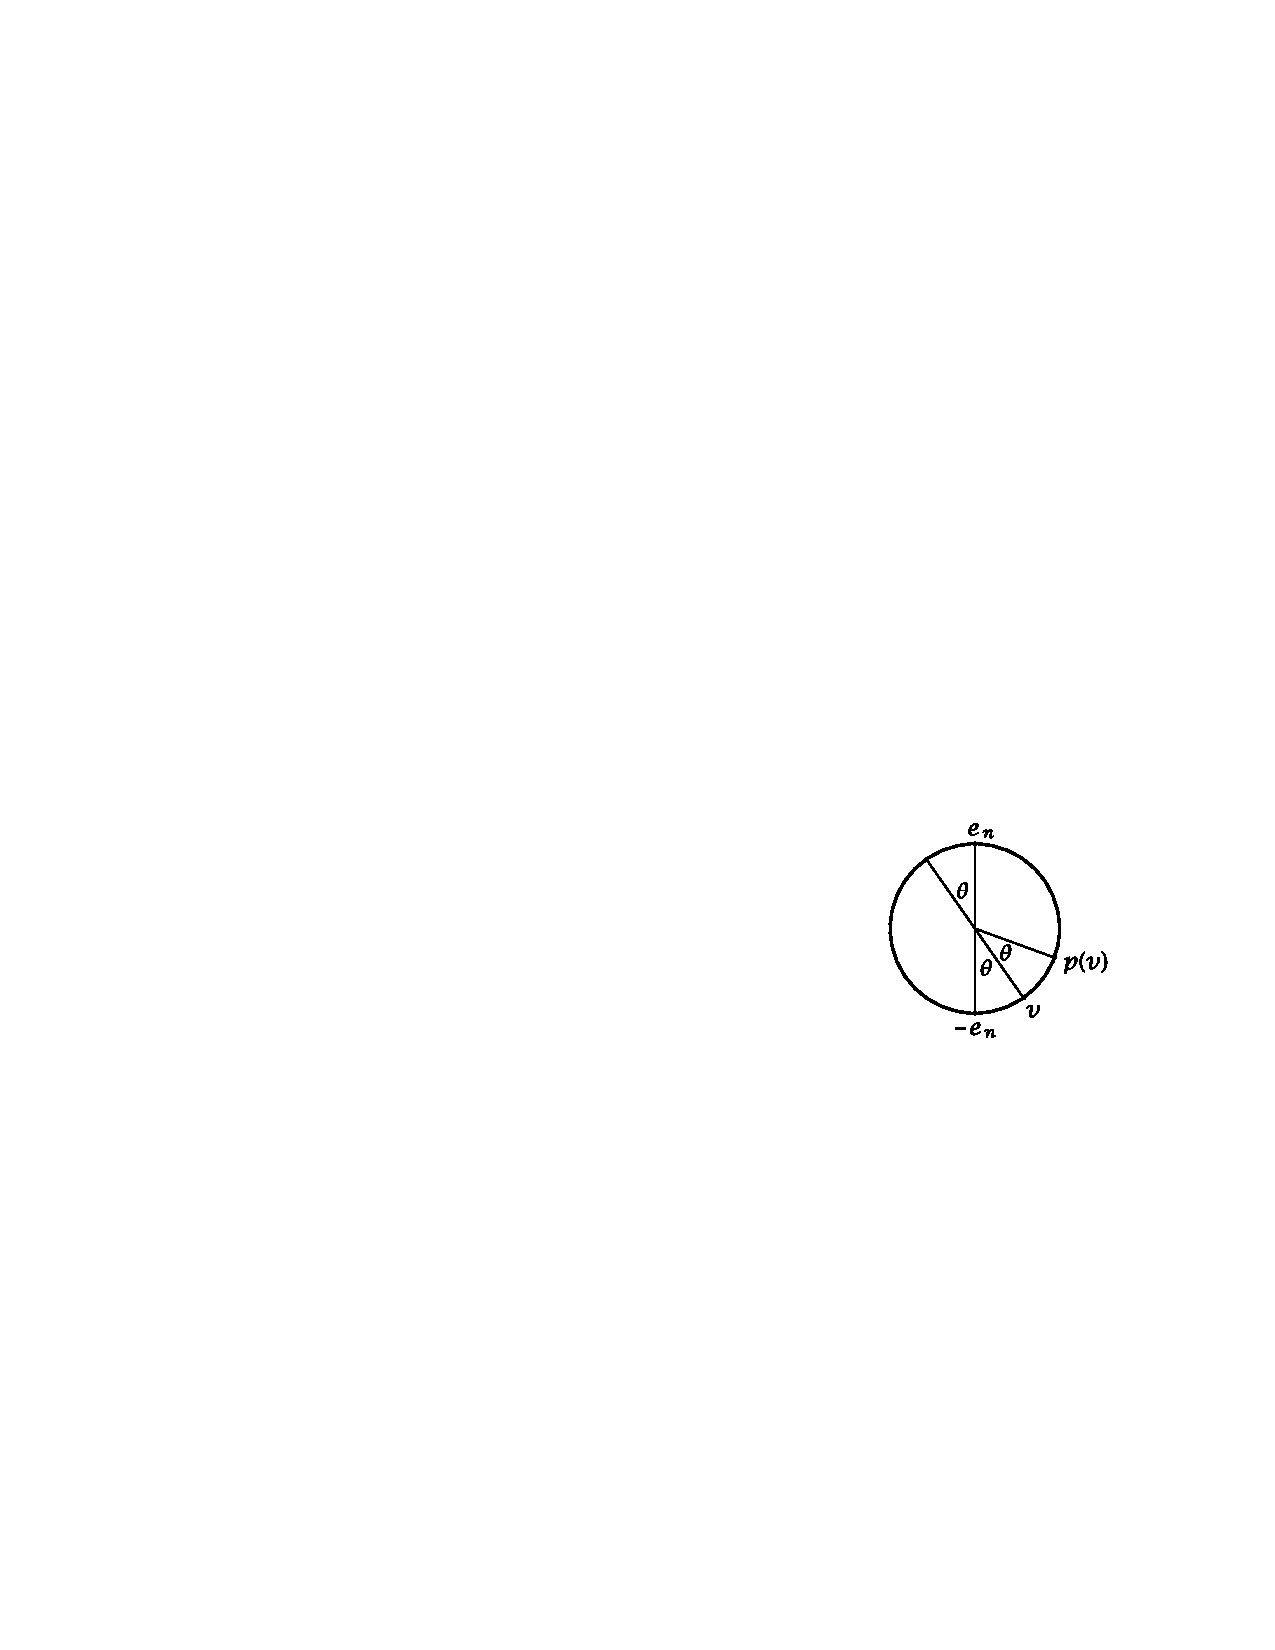
\includegraphics[scale=0.7]{Images/CW_SOn.pdf}
        \caption{Reflections defined in the proof of Proposition~\ref{prop 3D.1 Hatcher}.}
        \label{fig:CW_SOn}
    \end{figure}
    
    Statements (1) and (2) can now be proven by induction on $n$. The map $\rho$ takes $P^{n-2}$ to $\SO_{n-1}$, so we may assume inductively that the maps $\rho\circ\varphi^I$ for $I$ ranging over admissible sequences with first term $i_1<n-1$ are the characteristic maps for a $CW$-structure on $\SO_{n-1}$, with cells the corresponding products $e^I$. The admissible sequences $I$ with $i_1=n-1$ then give disjoint cells $e^I$ covering $\SO_n\setminus\SO_{n-1}$ by what was shown in the previous paragraph. So (1) and (2) hold for $\SO_n$.

    To prove (3) it suffices to show that there is an inclusion $P^iP^i\subset P^iP^{i-1}$ in $\SO_n$ since for an admissible sequence $I$, the map $\rho:P^I\to\SO_n$ takes the boundary of the top-dimensional cell of $P^I$ to the image of products $P^J$ with $J$ obtained from $I$ by decreasing one term $i_j$ by $1$, yielding a sequence which is admissible except perhaps for having two successive terms equal. As a preliminary to showing that $P^iP^i\subset P^iP^{i-1}$, observe that for $g\in \Or_n$ we have $r(g\cdot v)=gr(v)g^{-1}$. Hence $\rho(v)\rho(w)=r(v)r(e_1)r(w)r(e_1)=r(v)r(w')$ where $w'=r(e_1)\cdot w$. Thus to show $P^iP^i\subset P^iP^{i-1}$ it suffices to find for each pair $v,w\in\bbR^{i+1}$ a pair $x\in\bbR^{i+1}$, $y\in\bbR^i$ with $r(v)r(w)=r(x)r(y)$.

    Let $V\subset \bbR^{i+1}$ be a 2-dimensional subspace containing $v$ and $w$. Since $V\cap \bbR^i$ is at least 1-dimensional, we can choose a unit vector $y\in V\cap \bbR^i$. Let $g\in\Or_{i+1}$ take $V$ to $\bbR^2$ and $y$ to $e_1$. Then the conjugate $gr(v)r(w)g^{-1}=r(g\cdot v)r(g\cdot w)$ lies in $\SO_2$, hence has the form $\rho(z)=r(z)r(e_1)$ for some $z\in\bbR^2$ by statement (2) for $n=2$. Therefore
    \[r(v)r(w)=g^{-1}r(z)r(e_1)g=r(g^{-1}\cdot z)r(g^{-1}\cdot e_1)=r(x)r(y)\]
    for $x=g^{-1}\cdot z\in\bbR^{i+1}$ and $y\in\bbR^i$.

    It remains to show that the map $\rho:P^{n-1}\times P^{n-2}\times\cdots\times P^1\to \SO_n$ is cellular. This follows from the inclusions $P^iP^i\subset P^iP^{i-1}$ derived above, together with another family of inclusions $P^iP^j\subset P^j P^i$ for $i<j$. To prove the latter we have the formulas
    \begin{align}
        \rho(v)\rho(w)&=r(v)r(w')\text{ where }w'=r(e_1)\cdot w \notag\\
        &=r(v)r(w')r(v)r(v)\notag\\
        &=r(r(v)\cdot w')r(v)\text{ from }r(g\cdot v)=gr(v)g^{-1}\notag\\
        &=r(r(v)r(e_1)\cdot w)r(v)=r(\rho(v)\cdot w)r(v)\notag\\
        &=\rho(\rho(v)\cdot w)\rho(v')\text{ where }v'=r(e_1)\cdot v,\text{ hence }v=r(e_1)\cdot v'.
    \end{align}
    In particular, taking $v\in\bbR^{i+1}$ and $w\in\bbR^{j+1}$ with $i<j$, we have $\rho(v)\cdot w\in\bbR^{j+1}$, and the product $\rho(v)\rho(w)\in P^iP^j$ equals the product $\rho(\rho(v)\cdot w)\rho(v')\in P^jP^i$.
\end{proof}


This result can be used to easily compute the homology groups of $\SO_n$, as is done in \cite{Hatcher}. $CW$-structures also exist on $\SU_n$ and $\Sp_n$. We don't describe them since for us it will only be important to know that they exist. Instead of using these $CW$-structures directly, we will use exact sequences of homotopy groups to compute \emph{some} homotopy groups of the classical groups.





\subsection{Lie group actions I} \label{sec: Lie group actions}

\begin{defn}[Lie group action]\index{Lie group action}
    Given a Lie group $G$ and a smooth manifold $M$, a Lie group action of $G$ on $M$ is a smooth map $\Phi:G\times M\to M$ such that, denoting $\Phi_g=\Phi(g,\_):M\to M$, it holds that \[\Phi_e=\id_M,\] and either
    \[\Phi_{gh}=\Phi_g\circ \Phi_h\quad  \text{    (left action)}\]
    or
    \[\Phi_{gh}=\Phi_h\circ \Phi_g\quad  \text{(right action)}.\]

    In particular, each $\Phi_g$ is a diffeomorphism on $M$. As before, we will sometimes simply write $g\cdot x=\Phi(g,x)$ for left actions and $x\cdot g=\Phi(g,x)$ for right actions. The triple $(M,G,\Phi)$ is referred to as a Lie group action and the pair $(M,\Phi)$ as a $G$-manifold. When the name of the action is not needed, we will simply write $G\acts M$ for a left action and $M\lacts G$ for a right one.
\end{defn}

The notions of orbits, stabilizers, transitive actions and free actions transfer with no changes to the context of Lie groups.

\begin{example}[Actions of $G$ on itself]
    The left and right translation operators $L_g,R_g$ on a Lie group $G$ are smooth diffeomorphisms since $(L_g)^{-1}=L_{g^{-1}}$ is a smooth inverse. In addition,
    \[L_{gh}=L_g\circ L_h,\quad R_{gh}=R_h\circ R_g.\]
    Therefore $L_g$ defines a left action of $G$ on itself, and $R_g$ defines a right action. Note that these two actions commute: 
    \[L_g\circ R_h=R_h\circ L_g.\]
    
    In addition, the adjoint operator $\Adg_g$ defines the \emph{adjoint action} of $G$ on itself since 
    \[\Adg_{gh}=\Adg_g\circ \Adg_h,\]
    which makes it a left action. Similarly, $\Adg_{g^{-1}}$ is a right action.
\end{example}

\begin{example}[Lie group actions]
    \begin{enumerate}[label=(\alph*)]
        \item The natural action of $\GL_n(V)$ on $V$ via $(A,x)\mapsto Ax$ is a smooth left action.
        \item An action of a discrete group $\Gamma$ on a manifold is smooth iff every $\Phi_g$ is smooth. E.g.~$\bbZ^n$ acts smoothly and freely on $\bbR^n$ by translations $(n,x)\mapsto x+n$.
        \item The automorphism group $\Aut(\pi)$ of a smooth covering map $\pi:E\to M$ is a zero-dimensional Lie group acting smoothly and freely on $E$.
    \end{enumerate}
\end{example}

\begin{defn}[Equivariant maps]\index{Equivariant maps}
    Let $G$ be a Lie group, and let $(M,\Phi)$ and $(M',\Phi')$ be smooth manifolds endowed with smooth left or right $G$-actions $\Phi$ and $\Phi'$. A map $F:M\to M'$ is called $G$-equivariant with respect to the given $G$-actions if
    \[F\circ \Phi_g=\Phi_g' \circ F\]
    for all $g\in G$.
    In other words, the following diagram must commute:
    \[
    \begin{tikzcd}[every matrix/.append style={name=m}]
       M \arrow[r,"F"]\arrow[d,"\Phi_g",swap] & M'\arrow[d,"\Phi_g'"]\\
       M \arrow[r,"F", swap] & M'.
    \end{tikzcd}
    \]
    This condition is also often expressed by saying \emph{$F$ intertwines $\Phi$ and $\Phi'$}. Equivariant maps comprise the morphisms of the category $G\mathsf{-Man}^\infty$ of smooth manifolds with a $G$-action.

    Furthermore, for two Lie group actions $(M_i,G_i,\Phi^i)$, $i=1,2$, a morphism between them is a pair $(\varphi,\rho)$ consisting of a smooth map $F:M_1\to M_2$ and a Lie group homomorphism $\rho:G_1\to G_2$ such that the corresponding square commutes:
    \[F\circ \Phi^1=\Phi^2\circ \left(\rho\times F \right).\]
    In this case we say that $F$ intertwines the actions $\Phi^i,i=1,2$.
\end{defn}

\begin{example}
    The map $\exp:\bbR^n\to \bbT^n$ given by $\exp(x^1,\ldots,x^n)=(\rme^{2\pi\rmi x^1},\ldots,\rme^{2\pi\rmi x^n})$ is a smooth map that intertwines the actions of $\bbR$ on $\bbR^n$ and $\bbT^n$ by
    \begin{align}
        t\in\bbR\text{ acting on }\bbR^n:\;\quad t\cdot x&=x+tv,\\
        t\in\bbR\text{ acting on }\bbT^n:\; (t\cdot z)^k&=\rme^{2\pi\rmi tv^k}z^k,
    \end{align}
    where $v\in\bbR^n$ is a fixed vector.
\end{example}

\begin{thm}[Equivariant rank theorem {{\cite[Thm.~7.25]{Lee}}}]\label{thm equivariant rank}\index{Theorem!Equivariant rank}
    Let $F:(M,\Phi)\to F(M',\Phi')$ be a smooth $G$-equivariant map and let the action $\Phi$ be transitive. Then $F$ has constant rank.
\end{thm}
\begin{proof}
    Let $p,q\in M$, and let $g\in G$ be such that $\Phi_g(p)=q$ (it exists by transitivity). By computing the differential of the equivariance condition, we get
    \[T_qF\circ T_p\Phi_g=T_{F(p)}\Phi_g'\circ T_pF.\]
    Since the differentials of group actions are isomorphisms of vector spaces, the other two maps have the same rank. This means that $F$ has the same rank at any two points.
\end{proof}


\begin{defn}[Orbit map]\index{Orbit map}
    Given a Lie group action $\Phi:G\times M\to M$, for each $p\in M$ we define the smooth orbit map 
    \[\Phi^p:G\to M,\quad g\mapsto \Phi(g,p).\]
\end{defn}

\begin{prop}[{{\cite[Prop.~7.26]{Lee}}}]
    The orbit map $\Phi^p:G\to M$ defined above has constant rank, so the stabilizer $G_p=(\Phi^p)^{-1}(p)$ is a properly embedded Lie subgroup of $G$. If $G_p=\{e\}$, then $\Phi^p$ is an injective smooth immersion, so the orbit $\Phi(G,p)$ is an immersed submanifold of $M$.
\end{prop}
\begin{proof}
    First we note that $\Phi^p$ intertwines the left action of $L_g$ on $G$ and $\Phi$ on $M$. Since $G$ acts transitively on itself, $\Phi^p$ has constant rank by Theorem~\ref{thm equivariant rank}. Thus $G_p$ is properly embedded by Theorem~\ref{thm level set submanifold} and a Lie subgroup by Proposition~\ref{prop 7.11 Lee}.

    If $G_p=\{e\}$, then $\Phi^p$ is injective, and therefore by the Equivariant Rank Theorem~\ref{thm equivariant rank} it is a smooth immersion (recall that an injective map of constant rank is an immersion by the Global Rank Theorem~\ref{Global rank}). This makes the orbit an immersed submanifold by Proposition~\ref{prop 5.18 Lee}.
\end{proof}
\begin{rem}
    We will later prove that the condition on the stabilizer subgroup can be dropped.
\end{rem}

% \begin{example}[Classical groups]\index{Group!classical}
%     \begin{enumerate}[label=(\alph*)]
%         \item $\Or_n(\bbR)$ is the level set $F^{-1}(I_n)$ of the map $F:\GL_n(\bbR)\to \Mat_n(\bbR)$, $A\mapsto A^TA$. $F$ intertwines the right action of $\GL_n(\bbR)$ on itself with its right action $B\mapsto B^TAB$ on $\Mat_n(\bbR)$ (both actions are clearly smooth). Thus $\Or_n(\bbR)$ is a properly embedded Lie subgroup of $\GL_n(\bbR)$. It is compact because it is closed and bounded in $\Mat_n(\bbR)$: closed because it is a level set of $F$, and bounded because the matix norm of each orthogonal matrix is $\sqrt{n}$.
%         \item $\SO_n(\bbR)$ is the identity component of $\Or_n(\bbR)$, which is also the set of orthogonal determinant that have determinant $+1$ and thus preserve spatial orientations. Therefore it is an open Lie subgroup of $\Or_n(\bbR)$.
%         \item $U_n\subset \GL_n(\bbC)$ is defined similarly as the level set of $A\mapsto A^\ast A$ and is therefore a properly embedded Lie subgroup of $\GL_n(\bbC)$ of real dimension $n^2$. $\SU_n=\U_n\cap \SL_n(\bbC)$ and it is easy to check that $\SU_n$ is a properly embedded Lie subgroup of $U_n$ of real dimension $n^2-1$.
%     \end{enumerate}
% \end{example}







\subsection{Semidirect products}

\begin{defn}[Semidirect product]\index{Semidirect product}
    A smooth left action $\Phi:H\times N\to N$ of a Lie group $H$ on another Lie group $N$ is called an action by automorphisms if the maps $\Phi_h:N\to N$ are group automorphisms for all $h\in H$. 

    Given such an action, the semidirect product of $H$ and $N$ is, denoted $N\rtimes_\Phi H$ as a manifold, the Cartesian product $N\times H$, endowed with the multiplication
    \[(n,h)(n',h')=(n\Phi_h(n'),hh').\]
\end{defn}
It is easy to check that the product defined above is a valid group product, and it's clearly smooth along with its inverse $(n,h)^{-1}=(\Phi_h^{-1}(n^{-1}),h^{-1})$.

\begin{example}[The Euclidean group]\index{Group!Euclidean}
    $\Or_n(\bbR)$ acts by automorphisms on the translation group $\bbR^n$. Their semidirect product is the Euclidean group $E_n=\bbR^n\rtimes \Or_n(\bbR)$:
    \[(b,A)(b',A')=(n+An',AA').\]
    It also acts on $\bbR^n$ via 
    \[(b,A)\cdot x=b+Ax.\]
\end{example}


The following two theorems are a simple exercise.
\begin{prop}[Properties of semidirect products]
    Let $G=N\rtimes_\Phi H$ as above.
    \begin{enumerate}[label=(\alph*)]
        \item The subsets $\wt{N}=N\times\{e\}$ and $\wt{H}=\{e\}\times H$ are closed Lie subgroups of $G$ isomorphic to $N$ and $H$, respectively.
        \item $\wt N$ is a normal subgroup of $G$.
        \item $\wt N\cap \wt H=\{(e,e)\}$ and $\wt{N}\wt{H}=G$.
    \end{enumerate}
\end{prop}

\begin{thm}[Characterization of semidirect products]
    Let $N,H\subset G$ be closed Lie subgroups of a Lie group $G$ such that $N$ is normal, $N\cap H=\{e\}$, and $NH=G$. Then the map $(n,h)\mapsto nh$ is a Lie group isomorphism between $N\rtimes_{\Ad} H$ and $G$, where $\Ad:H\times N\to N$ is the adjoint action $\Ad_h(n)=hnh^{-1}$.
\end{thm}
This kind of a semiproduct is called \emph{internal}, but this theorem essentially shows that every semidirect product is internal with respect to the resulting group.

\begin{xca}
    Show the following isomorphisms:
    \begin{enumerate}[label=(\alph*)]
        \item $\Or_n(\bbR)\cong \SO_n(\bbR)\rtimes \Or_1$.
        \item $\U_n(\bbR)\cong \SU_n(\bbR)\rtimes \U_1$.
        \item $\GL_n(\bbR)\cong \SL_n(\bbR)\rtimes \bbR^\times$.
        \item $\GL_n(\bbC)\cong \SL_n(\bbC)\rtimes \bbC^\ast$.
    \end{enumerate}
    Prove that none of these groups are isomorphic to the analogous direct product groups by comparing the centers (the center is the set of all elements that commute with all of $G$).
\end{xca}





\subsection{Representations}

\begin{defn}[Linear representation]\index{Lie group!representation}
    Let $\bbK$ be either $\bbR$ or $\bbC$. A $\bbK$-linear representation of a Lie group $G$ is a $\bbK$-vector space $V$ with a smooth left $G$-action $\Phi$ such that each map $\Phi_g:V\to V$ is a $\bbK$-linear automorphism. Equivalently, a representation is a smooth homomorphism $\rho=\Phi_\bullet:G\to \GL_{\bbK}(V)$. 

    A representation $\rho :G\to \GL(V)$ is called \emph{faithful} if it is injective.
\end{defn}
Note that in principle it is possible do define infinite-dimensional representations even of finite-dimensional groups, but it will take some extra work to introduce the proper topology and smooth structure in that case.

\begin{example}[Lie group representations]
    \begin{enumerate}[label=(\alph*)]
        \item If $G$ is any Lie subgroup of $\GL_n(\bbR)$ (such groups are called \emph{matrix groups}), the inclusion map $G\hookrightarrow \GL_n(\bbR)$ is a faithful representation, called the \emph{defining representation of $G$}.
        \item The inclusion map $\bbS^1\hookrightarrow\bbC^\ast=\GL_1(\bbC)$ is a faithful representation of the circle group.
        \item Let $\sigma:\bbR^n\to \GL_{n+1}(\bbR)$ be the map that sends $x\in\bbR^n$ to the matrix $\sigma(x)$ defined in block form by 
        \[\sigma(x)=\begin{pmatrix}
            I_n & x\\
            0 & 1
        \end{pmatrix},\]
        where $I_n$ is the $n\times n$ identity matrix and $x$ is regarded as an $n\times 1$  column matrix. Then $\sigma$ is a faithful representation of the additive group $\bbR^n$.
        \item A faithful representation of the Euclidean group $E_n$ is given by $\rho:E_n\to \GL_{n+1}(\bbR)$ defined in block form by
        \[\rho(b,A)=\begin{pmatrix}
            A & b\\
            0 & 1
        \end{pmatrix},
        \]
        where $b$ is considered as a column.
        \item For positive integers $n$ and $d$, let $P^n_d$ denote the vector space of real polynomials $p:\bbR^n\to \bbR$ of degree at most $d$. For a matrix $A\in\GL_n(\bbR)$ define the linear map $\tau(A):P^n_d\to P^n_d$ by
        \[\tau(A)p=p\circ A^{-1}.\]
        This is a faithful representation of $\GL_n(\bbR)$.

        \item Another very important type of representation that is not linear is a projective representation, which is a homomorphism into the group $\PGL(V)=\GL(V)\slash (\bbK I)$ (where $\bbK I$ is the subgroup of multiplications by a scalar) of projective linear transformations of a vector space. The projective special linear group $\PSL_2(\bbC)=\SL_2(\bbC)\slash\{I,-I\}$, also isomorphic to the proper orthochronous Lorentz group $\SO^+(1,3)$, acts on the projective complex line $\bbC P^1\cong \bbC\cup\{\infty\}$ via M\"obius transformations
        \[\begin{pmatrix}
            a & b\\
            c& d
        \end{pmatrix} \cdot z=\frac{az+b}{cz+d}.\]
        It is easy to check that this is a left action. It is \emph{sharply 3-transitive}, meaning that for any triple of points $(z,w,x)$ there exists a unique matrix $g\in \PSL_2(\bbC)$ that maps them to $(0,1,\infty)$.
    \end{enumerate}
\end{example}

\begin{rem}
    Classical Lie groups are defined as groups of invertible matrices, and those matrices comprise the so called \emph{defining representations} of those groups. Moreover, very often in introductory courses on Lie groups it is assumed that all groups under consideration are matrix groups. It is therefore natural to ask whether every Lie group is isomorphic to some matrix group (such groups are also called \emph{linear}). The answer is no: not every finite-dimensional Lie group has a finite-dimensional faithful representation. The simplest example of a \emph{nonlinear} group is $\widetilde{\SL_2}(\bbR)$, the universal covering group of $\SL_2(\bbR)$. We will be able to show that it can't have a faithful representation later. Spin groups in even dimensions are also nonlinear. The fact of existence of such Lie groups is the ultimate justification for using general differential geometry to study them.
\end{rem}

Every Lie group has a canonical representation on its own tangent space at the identity.

\begin{defn}[Adjoint representation]\index{Adjoint representation}
    The derivative of the adjoint action at the identity, $T_e\Adg_g:T_e G\to T_e G$, is a linear representation of $G$. We use the same symbol without boldface to denote it:
    \[\Ad_g X=(\Adg_g)_{\ast e}(X).\]
    To further differentiate them, we will omit parentheses when writing the linear map $\Ad_g X$ but keep them when writing $\Adg_g(h)$.
\end{defn}

    Note that any abelian Lie group has a trivial adjoint representation ($\Ad_g=0$ for all $g\in G$).

\begin{example}[Adjoint representation of matrix groups]
    Let $G\subset \GL(V)$ be a matrix group. Then $T_e G\cong \Mat(V)$ and we can explicitly compute the adjoint representation. Since $\GL(V)$ is open in $\Mat(V)$, we can define a straight path $\gamma(t)=A+tX$ for any $A\in \GL(V)$ and $X\in \Mat(V)$. In particular, let $h(t)=I+tX$. Then for any $A\in \GL(V)$, using formula (\ref{eq differential in local coordinates}) for the action of a differential of a smooth map,
    \[\Ad_A X=\restr{\frac{\dd}{\dd t}}{t=0}A(I+tX)A^{-1}=AXA^{-1}.\]
    In other words, on matrix groups the Lie algebraic version of the adjoint map is still just matrix conjugation.
\end{example}






\subsection{Lie algebras: Construction I}

Since Lie groups are manifolds, the next most natural thing to do is to study its tangent spaces and to see what kind of structure on them is induced by the group structure. 
First we note that since $L_g:G\to G$ is a diffeomorphism for every $g\in G$, it induces the isomorphisms
\[(L_g)_{\ast e}: T_e G\to T_g G\]
between the tangent spaces at the identity and any other point. Moreover, since $L_{gh}=L_g\circ L_h$, the chain rule for derivatives implies that $(L_g)_\ast$ is natural in the sense that it truly depends only on $g$ itself and not how it might be decomposed into a product of other group elements.

Since Lie group homomorphisms preserve the identity, their derivatives map $T_e G$ to $T_eH$. Therefore it will completely suffice to study the properties of the tangent space at the identity.


First let us try to gain some intuition for how the group structure of $G$ might be ``encoded'' in $T_e G$ by working in local coordinates. Suppose $(U,\varphi)$ is a symmetric (i.e.~$U^{-1}=U$) open neighborhood of $e\in G$ and $\varphi:U\to \bbR^n$ a chart map on it such that $\varphi(e)=0$. We can find a smaller open neighborhood $U_0\subset U$ such that the the multiplication map $m:G\to G\to G$ restricts to $m:U_0\times U_0\to U$. The inversion map also restricts to $i:U\to U$. Then let $\mu:\varphi (U_0)^2\to \varphi(U)$ and $\iota:\varphi(U)\to \varphi(U)$ be their representatives in the local chart. Since these are now smooth maps on Euclidean spaces, we can study their Taylor series at the origin. Since $m(e,g)=m(g,e)=g$ for all $g$, we have
\[\mu(0,x)=\mu(x,0)=x\]
for all $x\in U_0$. This implies that both partial derivatives of $\mu$ computed at $(0,0)$ are the identity. Therefore the Taylor series of $\mu$ around the origin has the form
\[\mu(x,y)=x+y+\beta(x,y)+\gamma(x,y)+\calO(4),\]
where $\beta(x,y):\varphi(U_0)^2\to \bbR^n$ is some vector-valued bilinear form of $x,y\in\bbR^n$, $\gamma(x,y)$ is a similar cubic term, and $\calO(4)$ stands for terms that are quartic in $x$ and $y$ together ($x^4, x^3 y,$ etc.). In addition, since $m(g,i(g))=e$, we also have
\[\mu(x,\iota(x))=\mu(\iota(x),x)=0,\]
which implies that the Taylor series of the inversion map has the form
\[\iota(x)=-x+\beta(x,x)+\calO(x^3).\]

The extra constraints on the forms $\beta$ and $\gamma$ will come from the fact that they're not just some vector-valued forms, but that due to the group structure $m:G\times G\to G$ the domain and codomain of these forms are closely connected to each other. 



\begin{lem}
    The antisymmetric quadratic form
    \[b:\bbR^n\times\bbR^n\to \bbR^n,\quad b(x,y)=\beta(x,y)-\beta(y,x),\]
    is natural with respect to local coordinate transformations on $G$. That is, for any matrix $A\in\GL_n(\bbR)$,
    \[A b(x,y)=b(Ax,Ay).\]
\end{lem}
\begin{proof}
    Any local coordinate transformation on $U_0$, represented by a transition diffeomorphism $f$ with $f(0)=0$, will transform the local multiplication map $\mu$ into $\wt{\mu}$ with
    \[f(\wt\mu(x,y))=\mu(f(x),f(y)).\]
    Writing the Taylor series of $f$ as
    \[f(x)=Ax+f_2(x)+\calO(3),\]
    where $A$ is the Jacobi matrix of $f$ at the origin and $f_2(x)$ is the quadratic term, we have
    \[\mu(f(x),f(y))=Ax+Ay+f_2(x)+f_2(y)+\beta(Ax,Ay)+\calO(3)\]
    and
    \[f(\wt\mu(x,y))=Ax+Ay+A\wt\beta(x,y)+f_2(x+y)+\calO(3).\]
    By comparing these two expressions we conclude that
    \[f_2(x)+f_2(y)+\beta(Ax,Ay)=A\wt\beta(x,y)+f_2(x+y).\]
    In other words, the quadratic part of the multiplication map also depends on the quadratic part of the coordinate map itself. However, by noticing that the terms depending on $f_2$ are symmetric in $x$ and $y$, we get the statement of the theorem.
\end{proof}

This indicates the existence of a natural antisymmetric bilinear form $T_e G\times T_eG\to T_e G$. So far we have only used the property of the identity $eg=ge=g$. Aside from this, group multiplication also satisfies associativity.

\begin{lem}\label{3975}
    The associativity of group multiplication implies that
    \[
        \beta(\beta(x,y),z)+\gamma(x,y)+\gamma(x+y,z)
        =\beta(x,\beta(y,z))+\gamma(y,z)+\gamma(x,y+z).
    \]
\end{lem}
\begin{proof}
    We have 
    \begin{multline}
        \mu(\mu(x,y),z)=x+y+\beta(x,y)+\gamma(x,y)
        +z+\beta(x+y,z)+\beta(\beta(x,y),z)+\\+\gamma(x+y,z)+\calO(4)
    \end{multline}
    and 
    \begin{multline}
        \mu(x,\mu(y,z))=x+y+z+\beta(x,y+z)+\beta(y,z)
        +\gamma(y,z)+\beta(x,\beta(y,z))+\\+\gamma(x,y+z)+\calO(4).
    \end{multline}
    These two expressions must be equal by associativity. All terms of degree less than 3 cancel out because $\beta$ is bilinear, and we get the claimed formula.
\end{proof}

\begin{lem}
    The antisymmetric form $b(x,y)$ satisfies the Jacobi identity
    \[b(x,b(y,z))+b(y,b(z,x))+b(z,b(x,y))=0.\]
\end{lem}
\begin{proof}
    We antisymmetrize the equation from Lemma~\ref{3975} with respect to permutations of all three arguments. First we notice that the antisymmetrization of $\gamma(x,y)$ will be the same as that of $\gamma(y,z)$ since they are related to each other by a cyclic (and thus even) permutation. Moreover, the antisymmetizations of both $\gamma(x+y,z)$ and $\gamma(x,y+z)$ vanish since both of these are symmetric under a transposition of two of the arguments, and the only function that is both symmetric and antisymmetric is zero.

    What remains is 
    \[\calA \beta(\beta(x,y),z)=\calA \beta(x,\beta(y,z)),\]
    where $\calA$ is the antisymmetrization operator 
    \[\calA f(x_1,x_2,x_3)=\sum_{\sigma\in S_3}\sign(\sigma)f(x_{\sigma(1)},x_{\sigma(2)},x_{\sigma(3)}).\]

    This equation has six terms on each side, and we are going to group them into three groups of four by gathering terms that have the same variable standing alone. We start with those having $z$ as a lone variable. On the left hand side we combine two terms coming from the transposition $(1\Leftrightarrow2)$
    \[\beta(\beta(x,y),z)-\beta(\beta(y,x),z)=\beta(b(x,y),z),\]
    whereas on the right hand side we find
    \[\beta(z,\beta(x,y))-\beta(z,\beta(y,x))=\beta(z,b(x,y)).\]
    Finally, bringing these two expressions to the same side we find
    \[\beta(b(x,y),z)-\beta(z,b(x,y))=b(b(x,y),z).\]
    The full antisymmetrization is just a sum of cyclic permutations of this one, which gives us the Jacobi identity.
\end{proof}

\begin{rem}
    It's always possible to find some local coordinates in which $\beta(x,y)=\frac12 b(x,y)$ is antisymmetric right away (namely the coordinates in which $\iota(x)=-x+\calO(x^3)$). Later we will prove the miraculous result that there is a special coordinate system in which $\iota(x)\equiv-x$ and not only the quadratic term, but \emph{all} higher terms in the Taylor series of $\mu(x,y)$ can be written in terms of \emph{only} $b(x,y)$, and there is a \emph{universal} formula giving this dependence (the Baker-Campbell-Hausdorff formula). In other words, the entire local structure of the Lie group is encoded in the bilinear form $b$.
\end{rem}



\subsection{Lie algebras: Construction II}

The above calculations can be circumvented if we display a manifestly functorial object that gives an antisymmetric bilinear form on $T_eG$. To this end, let us take a look at the local representation of the conjugation map $\Ad_g h=ghg^{-1}$:
\[c(x,y)=\mu(\mu(x,y),\iota(x)).\]

\begin{lem}
    The Taylor series of the local conjugation map reads
    \[c(x,y)=y+b(x,y)+\calO(3).\]
\end{lem}
\begin{proof}
Combining the Taylor series of $\mu$ and $\iota$, we have
    \begin{multline}
        \mu(\mu(x,y),\iota(x))= x+y+\iota(x)+\beta(x+y,\iota(x)) +\beta(x,y)+\calO(3)=\\
        =x+y-x+\beta(x,x)+\beta(x,-x)+ \beta(y,-x)+ \beta(x,y)+\calO(3)=\\
        =y+\beta(x,y)-\beta(y,x) +\calO(3)=y+b(x,y)+\calO(3).
    \end{multline}
\end{proof}

Moreover, since $c(x,0)=0$ for all $x$ in some neighborhood of the origin, we know that the error term $\calO(3)$ vanishes when $y=0$ and therefore is $\calO(3)=y\calO(x^2,xy,y^2)$. This means that the double derivative with respect to $x$ and $y$, which naturally acts on two vectors $X,Y\in\bbR^n$ reads
\[\left(\frac{\partial^2}{\partial x\partial y}c(x,y)\right)(X,Y)=b(X,Y)+\calO(x,y)(X,Y).\]
At $x=y=0$ the error term vanishes and we get
\[\left(\restr{\frac{\partial^2}{\partial x\partial y}}{x=y=0}c(x,y)\right)(X,Y)=b(X,Y).\]

Obviously this double derivative is nothing but the local chart representation of the double derivative of $\Adg_g(h)= ghg^{-1}$ viewed as a map $G\times G\to G$ with respect to both variables. Recall that we call its derivative at the identity $(\Adg_g)_{\ast e}:T_eG\to T_e G$ by the symbol $\Ad_g$. We can now think of this as a map $\Ad_\bullet:G\to \GL(T_e G)$. With this, we have
\[T_{g=e}T_{h=e}(\Ad_g(h))=T_e \Ad_\bullet.\]
Note that the two derivatives commute because partial derivatives of smooth maps on $\bbR^n$ commute. This is a linear operator $T_e \Ad_\bullet:T_eG\to T_e\GL(T_e G)\cong \End(T_eG)$ from the tangent space $T_e G$ to the space of linear operators on it (this can also be thought of as a tensor on $T_e G$ of contravariant rank 1 and covariant rank 2).

\begin{defn}[Adjoint operator, Lie bracket]
    The linear adjoint operator is
    \[\ad=T_e \Ad: \quad T_eG\to \End(T_eG).\]
    More explicitly, for every $X,Y\in T_eG$, the action of $\ad_X:T_eG\to T_eG$ is defined by
    \[\ad_X Y=(T_e(\Ad_\bullet Y))(X).\]
\end{defn}

Equivalently, using the definition of tangent vectors as equivalence classes of curves, we have
\begin{multline}
    \ad_X Y=\restr{\frac{\dd}{\dd t} \frac{\dd}{\dd s}}{t=s=0}g(t)h(s)g^{-1}(t)=\restr{\frac{\dd}{\dd t} \frac{\dd}{\dd s}}{t=s=0}g(t)h(s)g^{-1}(t)h^{-1}(s)=\\=\restr{\frac{\dd}{\dd t} \frac{\dd}{\dd s}}{t=s=0}{} [g(t),h(s)].\label{30071}
\end{multline}
for any two curves $g(t)$ and $h(s)$ such that $X=g'(0)$ and $Y=h'(0)$. The fact that inserting the extra $h^{-1}(s)$ doesn't change the result is due to the fact that it can't contribute anything to the $\calO(ts)$ term in the Taylor series since the $\calO(t)$ term in $ghg^{-1}$ is already zero (to first order $ghg^{-1}$ in local coordinates reads $tX+sY-tX=sY$ as follows from our local functions $\mu$ and $\iota$). This identity can be treated as yet another construction of the Lie algebra, but we already know that it is equivalent to the others.

Note that in local coordinates the anti-symmetric form that we derived in the first construction is exactly the Lie bracket written in a local chart $(U,\varphi)$:
\[b(\varphi_{\ast e} X,\varphi_{\ast e} Y)=\varphi_{\ast e}(\ad_X Y).\]
The anti-symmetry and the Jacobi identity for $\ad_X Y$ follow from those for $b(X,Y)$.

\begin{defn}[Lie algebra]\index{Lie algebra}
    A Lie algebra is a pair $(\frakg,[\cdot,\cdot])$ where $\frakg$ is a finite-dimensional vector field over the field $\bbK$ and $[\cdot,\cdot]:\frakg\times\frakg\to\frakg$ is a map called a Lie bracket that satisfies the following properties for all $X,Y,Z\in \frakg$:
    \begin{enumerate}
        \item bilinearity: for all $a,b\in \bbK$,
        \[[aX+bY,Z]=a[X,Z]+b[Y,Z],\quad [X,aY+bZ]=a[X,Y]+b[X,Z];\]
        \item alternating property:
        \[[X,X]=0;\]
        \item Jacobi identity:
        \[[[X,Y],Z]+[[Y,Z],X]+[[Z,X],Y]=0.\]
    \end{enumerate}
    Note that over fields of characteristic other than 2, like $\bbR$ or $\bbC$ the last two properties together imply skew-symmetry (anticommutativity) $[X,Y]=-[Y,X]$.

    A Lie subalgebra of $\frakg$ is a linear subspace $\frakh\subset\frakg$ such that $[\frakh,\frakh]\subset\frakh$, i.e.~the restriction of the Lie bracket to $\frakh$ produces a Lie bracket on $\frakh$ and the inclusion map is a homomorphism of Lie algebras. In this case we write $\frakh\leq \frakg$.
\end{defn}


\begin{example}
    Any associative algebra $(A,\cdot)$ (i.e.~a vector space with a binary associative multiplication operation) can be endowed with a structure of a Lie group by setting the Lie bracket as the commutator
    \[[X,Y]=X\cdot Y-X\cdot Y.\]
    For example, the algebra $\Lin(V)=\End(V)$ of linear maps on a vector space $V$ admits this structure. In fact this is a forgetful functor $\mathsf{AssAlg}\to\mathsf{LieAlg}$.
\end{example}

Historically, most Lie algebras were ``discovered'' as not just the Lie algebras associated with associative rings (i.e.~commutator algebras), but as algebras of derivations on rings.

\begin{defn}[Derivation]\index{Derivation}
    Given a (not necessarily associative) ring $R$, a derivation on it is a map $D:R\to R$ that is additive ($D(x+y)=Dx+Dy$) and satisfies the Leibniz rule $D(xy)=Dx\cdot y+x\cdot Dy$.
\end{defn}

\begin{example}[Lie ring/algebra of derivations]
    Denote the set of all derivations on a ring $R$ by $\Der(R)$. Clearly the sum of two derivations is a derivation, however the composition is not always a derivation. However, it is easy to verify that the commutator $[D_1,D_2]=D_1D_2-D_2D_1$ of two derivations is a derivation. Thus $\Der(R)$ has a natural structure of a Lie ring. If $R=A$ is actually an algebra over some field, then $\Der(A)$ becomes a Lie algebra. As we will soon see, when $A$ is an algebra of smooth scalar functions, $\Der(A)$ consists of a certain type of differential operators.
\end{example}



\begin{defn}[Lie algebra homomorphism]
    Given two Lie algebras $\frakg,\frakg'$, a homomorphism $\phi:\frakg\to\frakg'$ is a linear map such that 
    \[\phi[X,Y]_{\frakg}=[\phi X,\phi Y]_{\frakg'}.\]
    These maps comprise the morphisms in the category $\mathsf{LieAlg}_{\bbK}$ of Lie algebras over the field $\bbK$.
\end{defn}


\begin{example}[Inner derivations on a Lie algebra]
    On any abstract Lie algebra $(\frakg,[\cdot,\cdot])$ one can define the linear adjoint operators $\ad_x:\frakg\to\frakg$ by $\ad_x(y)=[x,y]$. It is then easy to see that the Jacobi identity for $[\cdot,\cdot]$ is equivalent to the statement that $\ad_x$ is a derivation on $\frakg$:
    \[\ad_x([y,z])=[\ad_x y,z]+[y,\ad_x z].\]
    Moreover, since $\ad_x y=-\ad_y x$, this can also be written as
    \[\ad_{[x,y]}z=[\ad_x,\ad_y]z,\]
    which is equivalent to saying that $\ad:\frakg\to \mathfrak{gl}(\frakg)$ is a \emph{homomorphism} of Lie algebras. Therefore the set of all adjoint operators comprises a Lie subalgebra $\Inn(\frakg)\subset \mathfrak{gl}(\frakg)$, called the \emph{algebra of inner derivations} on $\frakg$.
\end{example}



Knowing from Construction I that $\ad_X Y$ satisfies the properties of a Lie bracket, we can finally define the Lie algebra corresponding to a Lie group.

\begin{defn}[Lie algebra of a Lie group]
    Given a Lie group $G$, its Lie algebra is $\frakg=T_e  G$ with the Lie bracket $[X,Y]=\ad_X Y$. 
    
    The Jacobi identity can be alternatively written as
    \[\ad_X[Y,Z]=[\ad_X Y,Z]+[Y,\ad_X Z],\]
    which is equivalent to saying that the adjoint $\ad_X$ is a derivation with respect to the Lie bracket.
\end{defn}

\begin{lem}\label{lem gl(V)}
    If $G=\GL(V)$ and $X,Y\in T_e G\cong \End(V)$, then 
    \[\ad_X Y=[X,Y]=XY-YX.\]
\end{lem}
\begin{proof}
    As we've shown before, on matrix groups $\Ad_A Y=AYA^{-1}$. Letting $A=I+tX$ and noting that $A^{-1}=I-tX+\calO(t^2)$, we find
    \[\Ad_{I+tX} Y=t(XY-YX)+\calO(t^2),\]
    which upon differentiation at $t=0$ implies the claimed formula.
\end{proof}


\begin{example}[$\mathfrak{gl}_n(R)$]
    The so called \emph{general linear Lie algebra} constructed in Lemma~\ref{lem gl(V)} is denoted $\mathfrak{gl}(V)=\End(V)^{(-)}$ (recall that $R\mapsto R^{(-)}$ is the forgetful functor that turns a ring into its associated Lie ring by defining the Lie bracket as the commutator). In fact it can be defined over all associative rings. Usually we use the standard basis consisting of the \emph{standard matrix units} $e_{ij},i\leq j$. Since $e_{jh}e_{ik}=\delta_{jh}e_{ik}$, the commutator reads
    \[[e_{ij},e_{hk}]=\delta_{jh}e_{ij}-\delta_{ki}e_{hj}.\]

    Later we will see that the Poincar\'e-Birkhoff-Witt Theorem implies that any Lie algebra $L$ is isomorphic to a subalgebra of some Lie algebra $A^{(-)}$ associated with some associative algebra $A$. Moreover, the theorem of Ado and Iwasawa implies that for a finite-dimensional $L$ the algebra $A$ can be taken to be finite-dimensional.
\end{example}

\begin{example}[$\mathfrak{sl}_n(R)$]
    The commutator of any two traceless matrices is traceless, thus we have the Lie subalgebra of $\mathfrak{gl}_n(R)$ consisting of traceless matrices:
    \[\mathfrak{sl}_n(R)=\{x\in \mathfrak{gl}_n(R)\mid \tr x=0\},\]
    called the \emph{special linear Lie algebra}.
\end{example}

\begin{xca}
    Come up with a way to embed $\mathfrak{gl}_n(R)$ as a Lie subalgebra of $\mathfrak{sl}_{n+1}(R)$.
\end{xca}


Now it is instructive to repeat the derivation of the properties of this Lie bracket without reference to local coordinates. First, we prove its naturality.

\begin{prop}[{{\cite[Prop.~1.1.3]{DK}}}]\label{prop 1.1.3 DK}
    Let $G,G'$ be Lie groups with corresponding Lie algebras $\frakg,\frakg'$, respectively, and suppose that $\Phi:G\to G'$ is a group homomorphism that is differentiable at $e\in G$. Write $\phi=T_e \Phi$. Then:
    \begin{enumerate}
        \item $\phi\circ \Ad_g=\Ad_{\Phi(g)}\circ \phi$ for any $g\in G$.
        \item $\phi:\frakg\to\frakg'$ is a homomorphism of Lie algebras.
    \end{enumerate}
\end{prop}
\begin{proof}
    Differentiating:
    \[\Phi(\Adg_g(h))=\Phi(ghg^{-1})=\Phi(g)\Phi(h)\Phi(g)^{-1}=\Adg_{\Phi(g)}(\Phi(h))\]
    with respect to $h$ at the identity in the direction of $Y$, we get
    \[\Phi_{\ast e} \Ad_g Y=\Ad_{\Phi(g)} \Phi_{\ast e}Y.\]
    Differentiating again with respect to $g$ at the identity in the direction of $X$ we get
    \[\Phi_{\ast e}([X,Y]_{\frakg})=[\Phi_{\ast e}X,\Phi_{\ast e}Y]_{\frakg'}\]
    as claimed.
\end{proof}
\begin{cor}
    The above Proposition shows that we have constructed a functor called the Lie functor:
    \[\Lief:\quad \mathsf{LieGr}\to \mathsf{LieAlg}\]
    that takes Lie groups to their Lie algebras and Lie group homomorphisms to their derivatives at the identity.
\end{cor}

\begin{rem}
    Following convention, we will use small Gothic letters to denote Lie algebras, for example $\frakg=\Lief G$.
\end{rem}

\begin{rem}
    Looking ahead, we will ultimately show that the Lie functor, under proper restrictions, becomes an equivalence of categories. Namely, homomorphisms between \emph{connected} Lie groups are uniquely determined by their derivatives at $e$, and every finite-dimensional Lie algebra has a unique simply connected Lie group corresponding to it. Taken together, these statements were originally proven by Sophus Lie and are sometimes called Lie's Fundamental Theorems.
\end{rem}


Now we are finally ready show (once again) that $\ad_X Y$ indeed satisfies the properties of a Lie bracket.

\begin{thm}
    Let $G$ be a Lie group and let $[X,Y]=\ad_X Y$ be the Lie bracket in the Lie algebra $\frakg=\Lief G$. Then for all $X,Y,Z\in\frakg$:
    \begin{gather}
        [X,Y]=-[Y,X],\\
        [[X,Y],Z]=[X,[Y,Z]]-[Y,[X,Z]].
    \end{gather}
\end{thm}
\begin{proof}
    $\Ad:G\to \GL(\frakg)$ is a smooth homomorphism, hence Proposition~\ref{prop 1.1.3 DK} shows that $\ad=T_e\Ad$ is a homomorphism of Lie algebras $\frakg\to \Lin(\frakg)$ (as usual, $\Lin(V)$ denotes the space all linear maps $V\to V$ in the category of vector spaces). Recall now that the Lie algebra on $\End(\frakg)$ is given by the commutator, therefore
    \[\ad_{[X,Y]}=\ad_X \ad_Y-\ad_Y \ad_X.\]
    Applying this to $Z\in\frakg$ we get the Jacobi identity. For skew-symmetry we observe that the group commutator 
    \[(g,h)\mapsto [g,h]=ghg^{-1}h^{-1}\]
    defines a smooth mapping $G\times G\to G$ whose derivative at $(e,e)$ is zero (this expresses the fact that $X+Y=Y+X$ in $\frakg$). As a consequence, its second-order derivative at $(e,e)$ is an intrinsically defined symmetric bilinear mapping from $(\frakg\times\frakg)\times(\frakg\times\frakg)$ into $\frakg$. The derivative of $[g,h]$ with respect to $h$ at $e$ in the direction of $Y\in\frakg$ is equal to $(\Ad_g-I)(Y)$. Then the derivative of this with respect to $g$ at $e$ in the direction of $X\in\frakg$ is equal to $\ad_X Y$. Applying these differentiations in the opposite order, we first get $(I-\Ad_h)(X)$, and then $-\ad_Y X$. Since the order of these differentiations doesn't actually matter for $C^2$ maps, we conclude skew-symmetry.
\end{proof}


\begin{example}[Lie algebras of $\SO_3(\bbR)$ and $\SU_2$]\label{example Lie algebras of so3 and su2}
    Continuing Example \ref{example su2 and so3}, 
    the Lie algebra of $\SO_3(\bbR)$ can clearly be identitifed with the Lie algebra of antisymmetric $3\times 3$ real matrices. Moreover, it can be identified with the Lie algebra $(\bbR^3,\times)$, where $\times$ is the vector product, via the isomorphism $\omega\mapsto A_{\omega}$ (see formula (\ref{eq R3->so(3) hom})). 
    
    The Lie algebra of $\SU_2$, denoted $\fraksu_2$, can be identified with the space
    \[\fraksu_2=\left\{
    \begin{pmatrix}
        i\alpha&\beta\\-\wb{\beta}&-i\alpha
    \end{pmatrix}
    \middle| \alpha\in\bbR,\beta\in\bbC
    \right\}\]
    of anti-selfadjoint traceless complex $2\times 2$ matrices. We identify this space with $\bbR^3\cong \bbR\times \bbC$. Using the notation from above for an element $g(a,b)\in\SU_2$, we get
    \[\Ad_{g(a,b)}=
    \begin{pmatrix}
        |a|^2-|b|^2&2\Im (a\wb{b}) & 2\Re(a\wb{b}) \\
        2\Im(ab) & \Re(a^2+b^2) & -\Im(a^2-b^2)\\
        -2\Re(ab) & \Im(a^2+b^2) & \Re(a^2-b^2)
    \end{pmatrix}.\label{eq Ad: su2->so3}
    \]
    This can be identified with a rotation matrix $R_n$ with
    \[n=\sign(\Re a)\frac{\arccos\left(2(\Re a)^2-1\right)}{\sqrt{1-(\Re a)^2}}
    \begin{pmatrix}
        \Im a\\ \Re b \\ \Im b
    \end{pmatrix}.
    \]
    It follows that the adjoint map defines a group homomorphism $\Ad:\SU_2\to \SO_3(\bbR)$ with kernel equal to $\{\pm I\}\cong \bbZ_2$, therefore this is a two-fold covering of $\SO_3(\bbR)$ with the 3-sphere, where antipodal points of the sphere are mapped to the same element of $\SO_3(\bbR)$. This once again leads to the diffeomorphism $\SO_3(\bbR)\cong \bbR P^3$.
\end{example}



\begin{example}
    As an example of how functoriality simplifies computations, recall the adjoint representation $\Ad_g=(\Adg_g)_{\ast e}:\frakg\to \frakg$. Since $\Adg_g$ is a Lie group isomorphism, we automatically conclude that $\Ad_g$ is a Lie algebra isomorphism, i.e.:
    \[\Ad_g[X,Y]=[\Ad_g X,\Ad_g Y].\]
\end{example}

\begin{example}[Adjoint representation of $\SO_3(\bbR)$]
    As we saw in Example~\ref{example Lie algebras of so3 and su2}, the adjoint representation $\Ad:\SU_2\to \GL(\fraksu_2)$ can be seen as a homomorphism $\Ad:\SU_2\to \SO_3(\bbR)$. Therefore its derivative $\ad:\fraksu_2\to \frakgl(\fraksu_2)$ can be seen as $\ad:\fraksu_2\to \frakso_3$. By linearizing formula (\ref{eq Ad: su2->so3}) near the identity, i.e.~by Taylor expanding it at a point
    \[g=
    \begin{pmatrix}
        1+i\alpha &\beta \\
        -\wb{\beta} & 1-i\alpha
    \end{pmatrix}+\calO(\alpha^2,|\beta|^2),
    \]
    we get 
    \[\ad:\quad \begin{pmatrix}
        i\alpha&\beta\\-\wb{\beta}&-i\alpha
    \end{pmatrix}\mapsto 
    \begin{pmatrix}
        0&-2\Im \beta & 2\Re\beta\\
        2\Im \beta & 0 & -2\alpha \\
        -2\Re\beta & 2\alpha & 0
    \end{pmatrix}.\label{eq ad: su2->so3}\]
    The factor of $2$ here is a manifestation of the fact that $\SU_2$ is a double cover of $\SO_3$.
\end{example}





\subsection{Lie subalgebras and ideals}

Assume now that $i:H\to G$ is an immersive Lie group homomorphism. By using translation isomorphisms this is equivalent to $i_{\ast e}:\Lief H\to \Lief G$ being injective. By functoriality it respects the Lie bracket, which means that $i_{\ast e}$ identifies $\Lief H$ with a Lie subalgebra of $\Lief G$. In other words, the following Proposition holds.

\begin{prop}
    If $H<G$ is an immersed Lie subgroup of a Lie group $G$, then $\Lief H$ is a Lie subalgebra of $\Lief G$.
\end{prop}

The obvious question is now: Does the converse hold? The answer turns out to be yes, but we will have to wait to prove it.

\begin{example}
    $\Lief (G\times H)\cong \Lief G\oplus \Lief H$.
\end{example}


\begin{defn}[Lie algebra representation]
    A representation of a Lie algebra $\frakg$ over a field $\bbK\in \{\bbR,\bbC\}$ is a $\bbK$-vector space $V$ with a $\bbK$-linear homomorphism of Lie algebras $\rho:(\frakg,[\cdot,\cdot])\to \mathfrak{gl}(V)$ where the Lie bracket on $\mathfrak{gl}(V)\cong \End(V)$ is the canonical commutator bracket.
\end{defn}

\begin{defn}[Adjoint representation of a Lie algebra]
    For any Lie algebra $\frakg$, its adjoint representation is defined by the homomorphism
    \[\ad:\frakg\to \Der(\frakg)\leq \mathfrak{gl}(\frakg),\quad X\mapsto \ad_X.\]
    The image of this homomorphism is $\Inn(\frakg)$, the algebra if inner derivations.
\end{defn}


\begin{example}[The Heisenberg group and algebra]\label{example Heisenberg group}
    Let $H_3$ be the group of real $3\times 3$ matrices of the form
    \[\begin{pmatrix}
        1&a&c\\0&1&b\\0&0&1
    \end{pmatrix}.\]
    Its Lie algebra has the basis $X,Y,Z$ where each of these matrices is zero except for a $1$ in the position of $a,b,c$, respectively. The Lie bracket on this basis is $[X,Y]=Z$, $[Y,Z]=[X,Z]=0$.
    
    Let $C^\infty(\bbR)$ be the vector space of all smooth functions on $\bbR$. We define a representation of the Heisenberg algebra $\frakh_3=\Lief{H_3}$ on this space via the following linear operators;
    \[\rho(X)f=\frac{\dd}{\dd x}f,\quad \rho(Y)f=xf,\quad \rho(Z)f=f.\]
    It is easy to check that this is indeed a representation of $\frakh$. In quantum mechanics the Heisenberg algebra consists of the position and momentum operators plus the identity.
\end{example}

\begin{xca}
    The standard basis for $\mathfrak{sl}_2(\bbK)$ is 
    \[e=\begin{pmatrix}
        0&1\\0&0
    \end{pmatrix},\quad h=\begin{pmatrix}
        1&0\\0&-1
    \end{pmatrix},
    \quad f=\begin{pmatrix}
        0&0\\1&0
    \end{pmatrix}.\]
    Compute the images of these vectors in the adjoint representation.
\end{xca}

\begin{example}
    \begin{enumerate}
        \item Every 1-dimensional subspace of a Lie algebra is a Lie subalgebra.
        \item All upper triangular matrices ($X_{ij}=0$ for $i>j$) form a subalgebra $\frakb_n(\bbK)$ of $\frakgl_n(\bbK)$. We will later identify this is the Borel subalgebra of $\frakgl_n(\bbK)$.
        \item All strictly upper triangular matrices ($X_{ij}=0$ for $i\geq j$) form a subalgebra $\frakn_n(\bbK)$ of $\frakgl_n(\bbK)$.
        \item All diagonal matrices form an abelian subalgebra $\frakd_n(\bbK)$ of $\frakgl_n(\bbK)$. We will later identify this is the Cartan subalgebra of $\frakgl_n(\bbK)$.
    \end{enumerate}
\end{example}



\begin{defn}[Ideal]\index{Ideal}
    An ideal of a Lie algebra $\frakg$ is a linear subspace $\frakn\subset\frakg$ such that
    \[[\frakg,\frakn]\subset \frakn.\]
    In other words, $\frakn$ must be stable under all inner derivations of $\frakg$. Note that an ideal is automatically a Lie subalgebra, but in this case we use the special notation $\frakn\sube \frakg$.
\end{defn}

\begin{prop}
    If $H\subset G$ is a normal immersed Lie subgroup, then $\Lief H\leq \Lief G$ is an ideal.
\end{prop}
\begin{proof}
    If $H$ is normal, $\Ad:G\to \GL(T_eG)$ takes values in the subgroup of $\GL(T_eG)$ that leaves $T_e H$ invariant. Hence the same applies to its derivative $\ad$.
\end{proof}

\begin{defn}[Normalizer of a Lie algebra]\index{Normalizer}
    The normalizer of a subset $S\subset \frakg$ is
    \[N_\frakg(S)=\{X\in\frakg\mid [X,S]\subset S\}.\]
    If $S$ is a Lie subalgebra, then this is exactly the largest Lie subalgebra in which $S$ is an ideal. A subalgebra is called self-normalizing if $N_\frakg(S)=S$.
\end{defn}

\begin{xca}
    \begin{enumerate}
         \item Prove that $\frakb_n(\bbK)$ and $\frakd_n(\bbK)$ are self-normalizing subalgebras of $\frakgl_n(\bbK)$. Calculate the normalizer of $\frakn_n(\bbK)$.
         \item $\fraksl_n(\bbK)$ is an ideal of $\frakgl_n(\bbK)$.
    \end{enumerate}
\end{xca}

\begin{defn}[Center of a Lie algebra]\index{Center}
    The center of a Lie algebra $\frakg$ is the set
    \[C(\frakg)=\{X\in\frakg\mid [X,\frakg]=\{0\}\}.\]
    It is automatically a Lie subalgebra of $\frakg$ by virtue of being the kernel of the Lie algebra homomorphism $\ad:\frakg\to \frakgl(\frakg)$.
\end{defn}

\begin{defn}[Centralizer]
    The centralizer of a subset $S\subset\frakg$ is the set
    \[C_\frakg(S)=\{X\in\frakg\mid [X,S]=\{0\}\}.\]
    It is automatically a Lie subalgebra.
\end{defn}

\begin{xca}
\begin{enumerate}
    \item The centralizer of an ideal in a Lie algebra is also an ideal.
    \item The kernel of any Lie algebra homomorphism is an ideal.
    \item if $A,B\sube\frakg$ are two ideals, then $A+B$ and $A\cap B$ are also ideals.
    \item If $A,B\sube \frakg$ are two ideals, then the commutator subspace $[A,B]=\{[a,b]\mid a\in A,b\in B\}$ is itself an ideal. This is in fact equivalent to the Jacobi identity.
    \item For $A,B,C\sube \frakg$, verify
    \[[A+B,C]=[A,C]+[B,C].\]
    Is it true that $[A\cap B,C]=[A,C]\cap [B,C]$?
    \item For $A,B,C\sube \frakg$, verify
    \[[[A,B],C]=[[B,C],A]+[[C,A],B].\]
    \item $\Inn(\frakg)$ is an ideal of $\Der(\frakg)$.
    \item The normalizer of the Lie algebra of a Lie group $G$ is the Lie algebra of the normalizer of $G$.
\end{enumerate}
\end{xca}

\begin{defn}[Quotient algebra]
    For an ideal $\frakn\sube\frakg$, one can define the quotient Lie algebra $\frakg\slash \frakn$ as the quotient of vector spaces (whose elements are all the subspaces of the form $X+\frakn$) with the Lie bracket
    \[[X+\frakn,Y+\frakn]=[X,Y]+\frakn.\]
\end{defn}

\begin{defn}[Simple Lie algebra]
    A Lie algebra $\frakg$ is called simple if it has no proper ideals (that is, ideals other than the trivial ones, $0$ and $\frakg$).
\end{defn}


\begin{xca}
    Show that the center $C(\frakg)$ cannot have codimension 1. What is the group-theoretic analog of this result?
\end{xca}


\begin{defn}[Semidirect product of Lie algebras]\index{Semidirect product}
    Let $\frakh\leq \frakg$ and $\frakn\sube \frakg$. We say that $\frakg$ is the semidirect product of $\frakh$ and $\frakn$ if the restriction of the canonical projection $\frakg\to \frakg\slash\frakn$ to $\frakh$ induces an isomorphism $\frakh\cong \frakg\slash\frakn$.

    Every semidirect product can be constructed as the modification of the direct sum of the Lie algebras $\frakh\oplus\frakn$ where for any $X\in \frakh$ and $Y\in\frakn$ we set $[X,Y]=\theta(X)Y$ with some Lie algebra homomorphism $\theta:\frakh\to \Der(\frakn)$.
\end{defn}

\begin{example}
    The algebra $\frakb_n(\bbK)$ of triangular matrices is the semi-direct product of the ideal $\frakn_n(\bbK)$ and the complementary subalgebra $\frakd_n(\bbK)$.
\end{example}





\subsection{Low-dimensional Lie algebras}

Recall that an ideal is a subspace that is stable under only inner derivations on $\frakg$. Moreover, $A\sube B\sube C$ doesn't imply $A\sube C$. These defects are corrected in the next concept.

\begin{defn}[Characteristic ideal]
    A subspace $\frakn\subset \frakg$ is called a characteristic ideal of the Lie algebra $\frakg$ if 
    \[\Der(\frakg)\cdot \frakn\subset \frakn,\]
    i.e.~it is stable under all derivations of $\frakg$. It is automatically an ideal.
\end{defn}

\begin{xca}
\begin{enumerate}
    \item A characteristic ideal of an ideal is an ideal.
    \item A characteristic ideal of a characteristic ideal is a characteristic ideal.
    \item If $A,B$ are two characteristic ideals of $\frakg$, then $[A,B]$ is one too.
    \item If $\frakn\sube \frakg$ is such that $[\frakn,\frakn]=\frakn$, then it is characteristic.
\end{enumerate}
\end{xca}

\begin{defn}[Structure constants]
    Let $e_1,\ldots,e_n$ be a basis of an $n$-dimensional Lie algebra $\frakg$ over a field $\bbK$. Then
    \[[e_i,e_j]=\sum_k c_{ij}^k e_k\]
    for some set of numbers $c_{ij}^k\in\bbK$ called the structure constants of $\frakg$.
\end{defn}

\begin{xca}
    Write down the two constraints on the structure constants imposed by the structure of the Lie algebra.
\end{xca}

\begin{example}[2-dimensional Lie algebra]
    Up to isomorphism, there is clearly only one non-abelian Lie algebra of dimension $2$. By scaling we can assume that it is spanned by two elements $x,y$ such that $[x,y]=y$. Thus any such Lie algebra is isomorphic to the algebra of matrices 
    \[M=\left\{\begin{pmatrix}
        \ast &\ast \\
        0&0
    \end{pmatrix}\right\},\]
    with $x=e_{11}, y=e_{12}$. From the viewpoint of Lie theory, this is the Lie algebra of the $(ax+b)$-group, the affine group of a line.
\end{example}

\begin{lem}
    All derivations of the two-dimensional non-abelian Lie algebra $M$ are inner.
\end{lem}
\begin{proof}
    Let $D\in\Der(M)$. Since $[M,M]$ is a characteristic ideal, $Dy\in[M,M]$ and thus $Dy=\lambda y$ for some $\lambda\in\bbK$. However, $\ad_{\lambda x}y=\lambda y$ so that $(D-\ad_{\lambda x})y=0$. Thus, modulo inner derivations, we can from the very start assume that $Dy=0$. Now
    \[[Dx,y]=[Dx,y]+[x,Dy]=D[x,y]=Dy=0\]
    and thus $Dx=\mu y$ for some $\mu\in\bbK$. But then $D=\ad_{-\mu y}$ is itself an inner derivation.
\end{proof}

\begin{lem}\label{lem 2}
    If the two-dimensional Lie algebra $M$ is an ideal $M\sube \frakg$, then it is a direct summand of $\frakg$.
\end{lem}
\begin{proof}
    As we know, $\frakn=C_\frakg(M)$ is an ideal of $\frakg$. Since the center of $M$ is trivial, $\frakn\cap M=0$. On the other hand, for any $x\in\frakg$ the restriction $\restr{\ad_x}{M}$ is a derivation of $M$ and thus, by the preceding lemma, is inner. Thus there exists $y\in M$ such that $\restr{\ad_x}{M}=\restr{\ad_y}{M}$. But then $\ad_{x-y}(M)=0$, hence $x-y\in \frakn$ and we have the decomposition $x=(x-y)+y\in \frakn\oplus M$.
\end{proof}


Now we are ready to classify all 3-dimensional Lie algebras. Let $s=\dim[\frakg,\frakg]$.
\begin{itemize}
    \item If $s=0$, then $\frakg$ is abelian.
    \item If $s=1$, we can assume that $[\frakg,\frakg]$ is generated by $z$. We distinguish two cases. If $z$ is non-central, then $\frakg$ is the direct sum of the non-abelian 2-dimensional algebra $M$ constructed above, and of the 1-dimensional algebra. If $z$ is central, ther exist $x,y$ such that $[x,y]=z$. Clearly $x,y,z$ must be linearly independent, so the algebra is isomorphic to the algebra of strictly upper-triangular matrices $\frakn_3(\bbK)$, which is the Heisenberg algebra $H_3(\bbK)$.
    \item If $s=2$, then $[\frakg,\frakg]$ must be abelian: if it isn't, by Lemma~\ref{lem 2} it must be a direct summand, and thus $s=1$, a contradiction. Thus we may assume that $[\frakg,\frakg]$ is generated by $y,z$ with $[y,z]=0$. Let $x\in \frakg\setminus[\frakg,\frakg]$. Then
    \[[x,y]=ay+bz,\quad [x,z]=cy+dz\]
    for some $a,b,c,d\in\bbK$ such that $ad-bc\neq 0$. Clearly one can replace the matrix $\begin{pmatrix}
        a&b\\c&d
    \end{pmatrix}$
    by a conjugate (which corresponds to a change of basis on $[\frakg,\frakg]$) or scale it (corresponding to rescaling $x$). Thus, when $\bbK$ is algebraically closed, this matrix can be reduced to one of the following Jordan forms:
    \[\begin{pmatrix}
        1&0\\
        0&\lambda
    \end{pmatrix},\quad 
    \begin{pmatrix}
        1&1\\
        0&1
    \end{pmatrix}.\]
    In other words, in the first case, there is a basis $x,y,z$ such that
    \[[x,y]=y,\quad [x,z]=\lambda z,\quad [y,z]=0,\]
    for some $\lambda\in\bbK^\ast$, and two such algebras with different $\lambda$'s are isomorphic iff $\lambda_1=\lambda_2^{\pm 1}$. For an infinite field this gives infinitely many non-isomorphic algebras. 

    In the second case, there exists a basis $x,y,z$ such that
    \[[x,y]=y,\quad [x,z]=y+z,\quad [y,z]=0.\]

    \item If $s=3$, the algebra $\frakg$ must be simple. When $\bbK$ is algebraically closed, there is only one such algebra, up to isomorphism, namely $\fraksl_2(\bbK)$. One can choose a basis of this algebra in such a way that 
    \[[x,y]=z,\quad [y,z]=x,\quad [z,x]=y.\]
    However, over a field that isn't algebraically closed, this algebra may have several non-isomorphic forms. For example, over $\bbK=\bbR$ there are exactly two non-isomorphic 3-dimensional simple algebras, namely $(\bbR^3,\times)$ and $\fraksl_2(\bbR)$.
\end{itemize}


\begin{xca}
    Show that all classical Lie algebras (that is, the algebras of matrices that preserve a non-degenerate bilinear form $B$ in the sense that $BX+X^tB=0$) over a field of characteristic 0 are simple with the exception of
    \[\frakso_4(\bbK)=\fraksl_2(\bbK)\oplus\fraksl_2(\bbK).\]

    To prove this, first show that, for $\mathrm{char}(\bbK)\neq 2$, the smallest ideal of $\fraksl_n(\bbK)$ containing any standard unit $e_{ij}$ is $\fraksl_n(\bbK)$ itself. Furthermore, letting $\mathrm{char}(K)=p$ and assuming that $p\neq 2$ and $p$ doesn't divide $n$, use this result to show that $\fraksl_n(K)$ is simple for any $n\geq 2$. 

    This argument breaks down when $p$ divides $n$: the trace of any scalar matrix ($\lambda I$) vanishes in this case. Since scalar matrices are central, it follows that $\fraksl_n(\bbK)$ has a 1-dimensional ideal, and thus cannot be simple.
\end{xca}






\subsection{(*) Infinite-dimensional Lie groups}\label{sec: inf-dim groups}


Many important groups, such as groups of diffeomorphisms, gauge groups, or loop groups, do not have the structure of a finite-dimensional manifold. However, they are still ``locally Euclidean'' in the sense that each point in them has a neighborhood that can be homeomorphically mapped onto a subset of an infinite-dimensional vector space. With a carefully defined smooth structure on that vector space, one can introduce the structure of an infinite-dimensional Lie group. However it is important to keep in mind that there is a huge variety of non-equivalent choices of topologies and smooth structures on infinite-dimensional spaces, so the particular definition will depend on the application. Here we will work with the most common class of infinite-dimensional Lie groups, which are locally modeled on Fr\'echet vector spaces.

Throughout this section we assume that $\bbK$ is either $\bbR$ or $\bbC$.

\begin{defn}[Seminorm]\index{Seminorm}
    A seminorm on a $\bbK$-vector space $V$ is a function $p:V\to [0,\infty)$ which satisfies all properties of a norm except positive definiteness. That is, $p(x)=0$ does not necessarily imply $x=0$. We also say that $p$ is \emph{not point-separating}.
\end{defn}

\begin{defn}[Separating family of seminorms]\index{Separating family}
    Given a seminorm $p$ on a $\bbK$-vector space $V$, let $N_p=\ker p=p^{-1}(0)$. Then the quotient $V_p=V\slash V_p$ is a normed space with $\lVert v+N_p\rVert=p(v)$. Denote by $\alpha_p:V\to V_p$ the corresponding quotient map.

    A family $\calP$ of seminorms on $V$ is called separating if 
    \[\forall p\in \calP \; p(v)=0 \Rightarrow v=0.\]
    This is equivalent to the map
    \[\alpha:V\to \prod_{p\in\calP}V_p,\quad v\mapsto (\alpha_p(v))_{p\in \calP},\]
    being injective.
\end{defn}

\begin{defn}[Locally convex topology]\index{Locally convex space}
    Recall that the initial topology defined on a set $X$ by a family of mappings $f_j:X\to X_j, j\in J$, into topological spaces $X_j$ is just the pre-image of the product topology under $f=\prod_{j\in J}:X\to \prod_{j\in J}X_j$.

    To each separating family $\calP$ of seminorms on $V$ we associate the initial topology $\tau_{\calP}$ on $V$ defined by the maps $\alpha_p:V\to V_p$ into the normed spaces $V_p$. We call it the locally convex topology on $V$ defined by $\calP$.

    Since $\calP$ is separating, this topology makes $V$ a Hausdorff space. It is also easy to show that $V$ is a topological vector space in the sense that addition and multiplication by scalars on $V$ are continuous maps. A topological vector space $(V,\tau_\calP)$ constructed this way is called a \emph{locally convex space}. As follows from the construction, each locally convex space is in particular a topological vector space which can be embedded into a product $\prod_{p\in \calP}V_p$ of normed spaces.
\end{defn}

\begin{defn}
    Some authors drop the requirement that $\calP$ be separating, in which case the resulting topology is not Hausdorff.
\end{defn}

\begin{defn}[Fr\'echet space]\index{Fr\'echet space}
    A locally convex space $V$ is called a Fr\'echet space is its topology can be defined by a countable family $\calP=\{p_n\}_{n=0}^\infty$ of seminorms and if $V$ is complete with respect to the compatible metric
    \[d(x,y)=\sum_{n=0}^\infty 2^{-n}\frac{p_n(x-y)}{1+p_n(x-y)}.\]
    This is equivalent to $V$ being complete with respect to $\{p_n\}_n$ (i.e.\ if a sequence $(x_i)_i\in V$ is Cauchy with respect to each seminorm $p_n$, then there is a $x\in V$ such that $\lim_{i\to\infty} p_n(x_i)=0$ for each $n$; equivalently, $\alpha_{p_n}(x_i)$ is a Cauchy sequence in $V_p$ for each $n$).
\end{defn}
\begin{rem}
    The introduction of a metric is not necessary for defining Fr\'echet spaces. In fact, a Fr\'echet space is simply a locally convex metrizable topological vector space that is complete as a topological vector space. Note that a metrizable space is complete\tablefootnote{We are omitting the details of how to define completeness for non-metrizable topological vector spaces. For example, the space $C^\infty_c(\bbR)$ of compactly supported smooth functions on the real line is a non-metrizable topological vector space. It is sequentially complete but can't be metrizable. Indeed, $C^\infty_c(\bbR)$ is the union of a countable set of closed linear subspaces, say of functions supported on $[-N,N]$. Each of these subspaces has empty interior in the topology of $C^\infty_c(\bbR)$, and by Baire's category theorem, if it were metrizable, such a union would have to also have an empty interior. This would contradict the fact that this union is the entire space, therefore it is not metrizable.} iff it is sequentially complete. The latter means that every Cauchy sequence has a limit, and a Cauchy sequence in a topological vector space is a sequence $(x_n)_n\in V$ such that for every open neighborhood $U\subset V$ of the origin, $x_n-x_m\in U$ for sufficiently large $n$ and $m$. This definition doesn't rely on the existence of any metric. However, since it is easy to check that $d(x,y)$ based on a separating family of seminorms $\{p_n\}$ defines a translation invariant metric on any locally convex space, it follows that these two definitions are equivalent. 
    
    Moreover, Fr\'echet spaces can also be defined as topological vector spaces whose topology can be induced by some translation-invariant metric.
\end{rem}

\begin{example}
    \begin{enumerate}[label=(\alph*)]
        \item Let $X$ be a topological space. For each compact $K\subset X$ we obtain a seminorm $p_K$ on $C(X,\bbR)$ by
        \[p_K(f)=\sup_{x\in K}|f(x)|.\]
        The family $\calP$ of these seminorms defines on $C(X,\bbR)$ the locally convex topology of uniform convergence on compact subsets of $X$. 
        
        In general, this is not a metrizable and thus not a Fr\'echet space. However if $X$ is compact, then we may take $K=X$ and obtain a norm on $C(X,\bbR)$, making all other seminorms redundant. In this case $C(X,\bbR)$ is a Banach space (a complete normed vector space).
        \item The preceding example can be generalized to the space $C(X,V)$, were $V$ is a locally convex space. We define for each compact $K\subset X$ and each continuous seminorm $q$ on $V$ a seminorm
        \[p_{K,q}(f)=\sup_{x\in K} q(f(x)).\]
        The family of these seminorms defines a locally convex topology on $C(X,V)$. In fact, it is not difficult to check that this topology coincides with the compact-open topology.
        \item If $X$ is locally compact and countable at infinity,\tablefootnote{A space is countably infinite if it is the union of countably many compact subspaces. This property is also called $\sigma$-compactness.} then there exists a sequence $K_n$ of compact subsets of $X$ with $\bigcup_n K_n$ and $K_n\subset \Int K_{n+1}$. We call such a sequence an \emph{exhaustion} of $X$. Then each compact subset $K\subset X$ lies in some $K_n$, so that each seminorm $p_K$ is dominated by some $p_{K_n}$. This implies that $C(X,\bbR)$ is metrizable (because the metric $d(x,y)$ can be defined in this case), and since it is also complete, it is a Fr\'echet space. It even is a Fr\'echet algebra in the sense that the multiplication is continuous.
        \item For any set $X$ the space $\bbR^X$ of all real-valued functions $X\to \bbR=\prod_{y\in \bbR} X$ is a locally convex space with respect to the product topology. This topology is defined by the seminorms $p_x(f)=|f(x)|$, $x\in X$. This space is complete, and it is metrizable iff $X$ is countable.
    \end{enumerate}
\end{example}

\begin{example}
    \begin{enumerate}[label=(\alph*)]
        \item Let $U\subset \bbR^n$ be an open subset and consider the algebra $C^\infty(U,\bbR)$. For each multiindex $m=(m_1,\ldots,m_n)\in\bbN_0^n$ with $|m|=m_1+\cdots+m_n$, we consider the differential operator
        \[D^m=D_1^{m_1}\cdots D_n^{m_n}=\frac{\partial^{|m|}}{{\partial_1^{m_1}\cdots \partial_n^{m_n}}}.\]
        For each $m$ and each compact subset $K\subset U$ we define a seminorm on $C^\infty(U,\bbR)$ by 
        \[p_{K,m}(f)=\sup_{x\in K}|D^mf(x)|.\]
        The family of these seminorms defines a locally convex topology on $C^\infty(U,\bbR)$.

        To obtain an exhaustion of $U$, we choose a norm $\lVert\cdot\rVert$ on $\bbR^n$ and consider the compact subsets
        \[K_n=\{x\in U\mid \lVert x\rVert\leq n, \dist(x,\bbR^n\setminus U)\geq 1/n\},\]
        where $\dist(x,\bbR^n\setminus U)=\inf_{y\in \bbR^n\setminus U} \lVert x-y\rVert$ is a continuous function. It is easy to see that $(K_n)_n$ is an exhaustion of $U$, so that the topology on $C^\infty(U,\bbR)$ can be defined by a countable set of seminorms. Moreover, $C^\infty(U,\bbR)$ is complete within respect to the corresponding metric and the multiplication on this algebra is continuous, so it is a Fr\'echet algebra.
        
        \item Let $M$ be a smooth $n$-dimensional manifold and consider the algebra $C^\infty(M,\bbR)$. If $(U,\varphi)$ is a chart of $M$, then $\varphi(U)$ is an open subset of $\bbR^n$, so that, in view of (a), we have a Fr\'echet algebra structure on $C^\infty(\varphi(U),\bbR)$. We now consider the map
        \[\Phi:C^\infty(M,\bbR)\hookrightarrow \prod_{\alpha}C^\infty(\varphi_\alpha(U_\alpha),\bbR),\quad f\mapsto (\restr{f}{U}\circ \varphi^{-1})_\alpha\]
        where $\alpha$ is an index enumerating all charts $(U_\alpha,\varphi_\alpha)$ in an atlas of $M$, and endow the right hand side with the product topology, turning it into a locally convex algebra (this is an easy exercise). Therefore the inverse image of this topology turns $C^\infty(M,\bbR)$ into a locally convex algebra.

        This description is convenient but not very explicit. To see how it can be defined by seminorms, note that for each compact $K\subset M$ for which there exists a chart $\varphi:U\to \bbR^n$ with $K\subset U$ and for each multiindex $m\in \bbN_0^n$ we have a seminorm
        \[p_{K,m}(f)=\sum_{x\in \varphi(K)}\lvert D^m(f\circ \varphi^{-1})\rvert.\]
        It is easy to see that these seminorms define the same topology on $C^\infty(M,\bbR)$ and that we obtain the structure of a Fr\'echet algebra on $C^\infty,\bbR)$. This is called the \emph{topology of local uniform convergence of all partial derivatives}.

        \item If $M$ is a finite-dimensional paracompact complex manifold, then we consider the algebra $\mathrm{Hol}(M,\bbC)$ of holomorphic functions on $M$ as a subalgebra of $C(M,\bbC)$, endowed with the topology of uniform convergence on compact subsets of $M$. This topology turns $\mathrm{Hol}(M,\bbC)$ into a Fr\'echet algebra. Moreover, one can show that the injective map $\mathrm{Hol}(M,\bbC)\hookrightarrow C^\infty(M,\bbC)$ is also a topological embedding.
    \end{enumerate}
\end{example}

\begin{defn}[Final locally convex topology]\index{Final locally convex topology}
    Given a family of linear maps $f_\alpha:V_\alpha\to V$ from locally convex spaces $V_\alpha$ to a vector space $V$, the final locally convex topology on $V$ for this family is the locally convex topology defined by all those seminorms $p$ on $V$ for which all compositions $p\circ f_\alpha$ are continuous seminorms on $V_\alpha$.

    This topology has the universal property that a linear map $\varphi:V\to W$ into a locally convex space $W$ is continuous iff all the maps $\varphi\circ f_\alpha$ are continuous.
\end{defn}

\begin{example}
    \begin{enumerate}[label=(\alph*)]
        \item Let $X$ be a locally compact space and $C_c(X,\bbR)$ the space of compactly supported continuous functions. For each compact subset $K\subset X$ we then have the natural inclusion
        \[\alpha_K: C_K(X,\bbR)\hookrightarrow C_c(X,\bbR),\]
        where $C_K(X,\bbR)$ is the subspace consisting of functions supported on $K$. Each space $C_K(X,\bbR)$ is a Banach space with respect to the sup-norm $\lvert f\rVert_\infty$. We then endow $C_c(X,\bbR)$ with the final locally convex topology defined by the maps $\alpha_K$.
        
        \item Let $M$ be a smooth manifold and consider the space $C_c^\infty(M,\bbR)$ of compactly supported smooth functions. For each compact $K\subset M$ we have a natural inclusion
        \[\alpha_K: C_K^\infty(M,\bbR)\hookrightarrow C_c^\infty(M,\bbR).\]
        we endow each space $C^\infty_K(M,\bbR)$ with the subspace topology inherited from $C^\infty(M,\bbR)$, which turns it into a Fr\'echet space. We then endow $C_c^\infty(M,\bbR)$ with the final locally convex topology defined by the maps $\alpha_K$.
    \end{enumerate}
\end{example}

\begin{defn}[Calculus on locally convex spaces]\index{Derivatives on locally conves spaces}
    Let $X,Y$ be topological vector spaces, $U\subset X$ open and $f:U\to Y$ a map. Then the \emph{directional derivative} of $f$ with respect to $h\in X$ is
    \[\dd f(x)(h)=\lim_{t\to 0}\frac{1}{t}\left(f(x+th)-f(x)\right)\]
    whenever the limit exists. The function $f$ is called \emph{differentiable} if $\dd f(x)(h)$ exists for all $h\in X$, It is called \emph{continuously differentiable} if it is differentiable at all points of $U$ and 
    \[\dd f:U\times X\to Y,\quad (x,h)\mapsto \dd f(x)(h)\]
    is a continuous map. It is called a $C^1$-map if it is continuous and continuously differentiable, a $C^n$-map if $\dd f$ is a $C^{n-1}$-map, and a $C^\infty$- (or smooth) map if it is $C^n$ for all $n\geq 1$.

    if $X$ and $Y$ are complex vector spaces, then the map $f$ is called \emph{holomorphic} if it is $C^1$ and for all $x\in U$ the map $\dd f(x):X\to Y$ is complex linear (we will show that $\dd f$ is always real linear).
\end{defn}
\begin{rem}
    The existence of linear maps (which are always differentiable in the above sense) that are not continuous in the infinite-dimensional case shows that continuity of $f$ does not follow from its differentiability.
\end{rem}

\begin{lem}
\begin{enumerate}[label=(\roman*)]
    Let $X,Y$ be locally convex spaces, $U\subset X$ open and $f:U\to Y$ a continuously differentiable map. Then:
    \item For any $x\in U$ the map $\dd f(x):X\to Y$ is real linear and continuous.
    \item (Fundamental Theorem of Calculus) If $x+[0,1]h\subset U$, then
    \[f(x+h)=f(x)+\int_0^1 \dd f(x+th)(h)\dd t.\]
    In particular, $f$ is locally constant iff $\dd f=0$.
    \item $f$ is continuous.
    \item If $f$ is $C^n$, $n\geq 2$, then the functions $(h_1,\ldots,h_n)\mapsto \dd^nf(x)(h_1,\ldots,h_n)$, $x\in U$, are symmetric $n$-linear maps.
    \item If $x+[0,1]h\subset U$, then we have the Taylor formula
    \begin{multline}
        f(x+h)=f(x)+\dd f(x)(h)+\cdots +\frac{1}{(n-1)!}\dd^{n-1}f(x)(h,\ldots,h)+\\
        +\frac{1}{(n-1)!}\int_0^1 (1-t)^{n-1}\dd^n f(x+th)(h,\ldots,h)\dd t.
    \end{multline}
\end{enumerate}
\end{lem}
\begin{proof}
    \begin{enumerate}[label=(\roman*)]
        \item For each linear functional $\lambda\in Y^\ast$ and $h_1,h_2\in X$ the map
        \[F(t_1,t_2)=\lambda(f(x+t_1h_1+t_2h_2))\]
        is defined on an open neighborhood of the origin in $\bbR^2$ and has continuous partial derivatives 
        \[\partial_{t_i}F=\dd f(x+t_1h_1+t_2h_2)(h_i),\; i=1,2.\]
        From finite-dimensional calculus we know that $F$ is a $C^1$-map and $\dd F(0,0):\bbR^2\to \bbR$ is linear. This implies that $\lambda\circ \dd f(x)$ is linear on $\mathrm{Span}(h_1,h_2)$. Since $Y\ast$ separates the points of $Y$ (i.e.\ the pairing with the dual space is non-degenerate by definition) and $h_1,h_2$ are arbitrary, the map $\dd f(x)$ is real linear. Its continuity follows from the continuity of $\dd f$.

        \item We consider for $\lambda \in Y^\ast$ the $C^1$-map
        \[F:I\to \bbR,\quad F(t)=\lambda(f(x+th))\]
        and obtain from the Fundamental Theorem in single-variable calculus
        \[\lambda(f(x+h)-f(x))=F(1)-F(0)=\int_0^1 F'(t)\dd t=\int_0^1 \lambda(\dd f(x+th)(h))\dd t.\]
        Since $Y^\ast$ separates the points of $Y$, this implies that the weak integral $\int_0^1 \dd f(x+th)(h)\dd t$, which a priori exists only in the completion of $Y$, actually defines an element of $Y$ which coincides with $f(x+h)-f(x)$.

        \item Let $p$ be a continuous seminorm on $Y$ and $\epsilon>0$. Then there exists a balanced neighborhood (i.e.\ one that is invariant under multiplications by scalars $a$ such that $|a|\leq 1$) of the origin $U_1\subset X$ with $x+U_1\subset U$ and $p(\dd f(x+th)(h))<\epsilon$ for $t\in[0,1]$ and $h\in U_1$. Hence
        \[p(f(x+h)-f(x))\leq \int_0^1 p(\dd f(x+th)(h))\dd t\leq \epsilon\]
        (this is an easy exercise), and this $f$ is continuous.
        
        \item Arguing as in (i), we may \gls{wlog} assume that $Y=\bbR$. That the maps $\dd^n f(x)$ are symmetric and linear follows by considering maps of the form
        \[(t_1,\ldots,t_n)\mapsto f(x+t_1h_1+\cdots t_nh_n)\]
        on an open neighborhood of the origin in $\bbR^n$ and then applying the corresponding finite-dimensional result.
        
        \item We consider the $C^n$-map
        \[F:I\to \bbR, \quad F(t)=f(x+th), \quad F^{(n)}(t)=\dd^n f(x+th)(h,\ldots,h)\]
        and apply the Taylor formula for $C^n$-functions $I\to \bbR$.
    \end{enumerate}
\end{proof}

From these properties, one can similarly derive the rest of the classic theorems of calculus, such as the chain rule
\[\dd(g\circ f)(x)=\dd g(f(x))\circ \dd f(x),\]
and the equivalence of the $C^1$ property on the product space $X_1\times X_2$ to the continuity of partial derivatives $\dd_1f(x_1,x_2)$ and $\dd_2 f(x_1,x_2)$. We refer the reader to \cite[Sec.~II]{Neeb} for details.

\begin{rem}
The following properties immediately follows from these theorems.
\begin{enumerate}[label=(\alph*)]
    \item Continuous linear maps between locally convex spaces are smooth.
    \item The addition map $+:X\times X\to X$ on topological vector spaces is smooth.
    \item Continuous $k$-linear maps $m:X_1\times\cdots\times X_k\to Y$ are smooth.
    \item Assuming $f\in C^n$, $f$ is $C^{n+1}$ iff $\dd^n f$ is $C^1$.
    \item If $f:U\to Y$ is holomorphic, then $\dd f:U\times X\to Y$ is also holomorphic (since from finite-dimensional theory each map $x\mapsto \dd f(x)(h)$ is holomorphic).
\end{enumerate}
\end{rem}


\begin{rem}
    The assumption of local convexity in the definition of $C^1$-maps is crucial for the validity of the Fundamental Theorem. Without local convexity, it is possible to construct non-constant ``$C^1$'' paths $\gamma:I\to X$ such that $\dd \gamma=0$.

    In the context of Banach spaces, one further has an Inverse Mapping Theorem and an Implicit Mapping Theorem. Such results cannot be expected in general for Fr\'echet spaces (e.g.\ the exponential function on the group $\Diff(\bbS^1)$ of diffeomorphisms of the circle). Nevertheless, there is an Implicit Mapping Theorem for maps of the type $E\to F$, where $F$ is Banach and $E$ is locally convex.
\end{rem}

\begin{rem}[Pathologies of linear ODEs in Fr\'echet spaces]
    \begin{enumerate}[label=(\alph*)]
        \item Consider the Fr\'echet space $V=C^\infty([0,1],\bbR)$ and the continuous linear operator $Lf=f'$ on $V$. We are asking for solutions of the initial value problem
        \[\gamma'(t)=L\gamma(t), \quad \gamma(0)=\gamma_0\in V.\label{194}\]
        As a consequence of Borel's Theorem that each power series is the Taylor series of some smooth function, each $\gamma_0$ has a smooth extension to a function on $\bbR$. Let $h$ be such a function and consider
        \[\gamma:\bbR\to V, \quad \gamma(t)(x)=h(t+x).\]
        Then $\gamma(0)=\restr{h}{[0,1]}=\gamma_0$ and $\gamma'(t)(x)=h'(t+x)=(L\gamma(t))(x)$. It is clear that these solutions depend on the choice of the extension $h$. Therefore solutions to such initial problem values are not unique in Fr\'echet spaces, unlike in the finite-dimensional case.
        
        \item Now we consider $V=C^\infty(\bbS^1,\bbC)$ identified with the space of $2\pi$-periodic smooth functions on the real line. We consider the linear operator $Lf=-f''$ and the same equation~(\ref{194}), which in this case is the heat equation with reversed time. It is easy to analyze this equation in terms of the Fourier expansion of $\gamma$. Let
        \[\gamma(t)(x)=\sum_{n\in \bbZ} a_n(t)\rme^{\rmi nx}\]
        be the Fourier series for $\gamma(t)$. Then equation~(\ref{194}) implies $a_n'(t)=n^2a_n(t)$ for each $n\in\bbZ$, so, $a_n(t)=a_n(0)\rme^{tn^2}$ for any solution $\gamma$. If the Fourier coefficients $a_n(0)$ of $\gamma$ do not satisfy
        \[\sum_n |a_n(0)|\rme^{\epsilon n^2}<\infty\]
        for some $\epsilon>0$ (which need not be the case for a smooth function $\gamma_0$), then the initial value problem (\ref{194}) has no solutions on $[0,\epsilon]$.

        As a consequence, the operator $\exp(L)$ is never defined for $t\neq 0$. Nevertheless, we may use the Fourier series to see that $\beta(t)=(1+it^2)I+tL$ (where $I$ is the identity operator) defines a curve $\beta:\bbR\to \GL(V)$ which is smooth in the sense that 
        \[\bbR\times V\to V\times V,\quad (t,v)\mapsto (\beta(t)(v),\beta(t)^{-1}(v)\]
        is smooth. We further have $\beta'(0)=L$, so that $L$ arises as the tangent vector of a smooth curve in $\GL(V)$, but not for a one-parameter group.
    \end{enumerate}
\end{rem}

\begin{defn}[Mackey complete space]\index{Mackey complete space}
    A locally convex space $E$ is called Mackey complete if for each sooth curve $\xi:[0,1]\to E$ there exists a smooth curve $\eta:[0,1]\to E$ with $\eta'=\xi$.
\end{defn}

\begin{rem}
    If $E$ is a sequentially complete locally convex space (e.g.~a Fr\'echet space), then it is Mackey complete because sequential completeness implies the existence of Riemann integrals of continuous $E$-valued functions on compact intervals, hence that we can put $\eta(t)=\int_0^t \xi(s)\dd s$ and then $\eta'=\xi$.
\end{rem}

\begin{defn}[Infinite-dimensional smooth manifold]\index{Fr\'echet manifold}
    Let $M$ be a Hausdorff topological space and $E$ a locally convex space. An $E$-chart of an open subset $U\subset M$ is a homeomorphism $\varphi:U\to \varphi(U)\subset E$ into an open subset $\varphi(U)$ of $E$. Two charts $(U_\alpha,\varphi_\alpha)$ and $(U_\beta,\varphi_\beta)$ are called smoothly compatible  if the map
    \[\varphi_\beta\circ\varphi_\alpha^{-1}:\varphi_\alpha(U_{\alpha\beta})\to \varphi_\beta(U_{\alpha\beta})\]
    is smooth. From the chain rule it follows that compatibility of charts is an equivalence relation on the set of all $E$-charts. An $E$-atlas is a family of pairwise compatible $E$-charts that cover all of $M$. A smooth $E$-structure $\mathcal{A}$ on $M$ is a maximal $E$-atlas. A smooth $E$-manifold is a pair $(M,\mathcal{A})$ where $\mathcal{A}$ is a smooth $E$-structure on $M$.

    We call a manifold modeled on a locally convex, resp., Fr\'echet space, resp., Banach space a locally convex, resp., Fr\'echet, resp., Banach manifold.
\end{defn}

All of differential geometry that we will cover for finite-dimensional smooth manifolds translates without changes to the case of manifolds modeled on locally convex spaces. This includes tensor bundles, differential forms, Lie derivatives, exterior derivatives, and formulas relating them. However, results involving integration, such as the definition of integrals of differential forms, Stokes' theorem, and Poincar\'e lemma, require Mackey completeness.


\begin{defn}[Locally convex Lie group]\index{Locally convex Lie group}\index{Lie group!locally convex}
    A locally convex Lie group is a locally convex manifold endowed with a group structure such that the multiplication and the inversion maps are smooth.
\end{defn}

\begin{example}
    \begin{enumerate}[label=(\alph*)]
        \item (Vector groups) Each locally convex space $V$ is an abelian Lie group with respect to addition.
        \item (Diffeomorphism groups) For a compact finite-dimensional manifold $M$, the group $\Diff(M)$ of its diffeomorphisms can be turned into a locally convex Lie group modeled on the space $\fX(M)$ of smooth vector fields on $M$. Since we have not yet defined this space, the details of example will have to wait, but it will be useful to keep in mind for some of the discussions.
    \end{enumerate}
\end{example}











\newpage
\section{Fiber Bundles}\label{sec: Fiber bundles}

\subsection{Bundles}

Recall that by the Rank Theorem~\ref{Rank thm}, all submersions when restricted to sufficiently small neighborhoods in the domain look like projections in a direct product. Fiber bundles are a natural special case of this, where the submersion looks like a projection ``locally in the target'', i.e.~is a locally trivial map. 

\begin{defn}[Topological fiber bundle]\index{Fiber bundle!topological}
    A topological fiber bundle is continuous locally trivial map $\pi:E\to B$. The local trivializations $\varphi_\alpha:\pi^{-1}(U_\alpha)\to U_\alpha\times F$ are called \emph{bundle chart maps}. The set of those $b\in B$ for which the \emph{fiber} $\pi^{-1}(b)$ is homeomorphic to a fixed space $F$ is open and closed in $B$. Therefore it usually suffices to fix the homeomorphism type of the fibers. If all fibers are homeomorphic to $F$, we call $F$ the \emph{typical, or model, fiber}.
\end{defn}

From this definition it is clear that topological covering maps are exactly the topological fiber bundles with discrete fibers. Also by Theorem~\ref{thm local fibration}, every fiber bundle is a fibration, which we state as a Corollary. 

\begin{cor}[{{\cite[Cor.~3.2.5]{RS2}}}]
    Topological fiber bundles are Serre fibrations.
\end{cor}

This implies that all of our topological results for Serre fibrations will also hold for fiber bundles, most importantly the long exact sequence of homotopy groups. If the base space happens to be paracompact, one has the following stronger result.

\begin{cor}[Huebsch and Hurewicz {{\cite[Prop.~3.2.6]{RS2}}}]
    Topological fiber bundles over paracompact Hausdorff base spaces are Hurewicz fibrations.
\end{cor}
\begin{proof}
    See \cite[\S13.4]{tomDieck}.
\end{proof}

This will property will obviously survive in the smooth category since all manifolds are paracompact.

\begin{defn}[Smooth fiber bundle/locally trivial fibration]\index{Fiber bundle!smooth}
    A map $\pi\in C^\infty(E,M)$ is a locally trivial fibration, or a \gls{fb}, if it is a smooth submersion and for any $p\in M$ there is an open neighborhood $U_p$ and a diffeomorphism $\chi_p:\pi^{-1}(U_p)\to U_p\times \pi^{-1}(p)$ (recall that $\pi^{-1}(p)$ is a smooth manifold for submersions) such that the following triangle commutes:
    \[
    \begin{tikzcd}[every matrix/.append style={name=m},   
    execute at end picture={\draw [<-] ([xshift=0mm,yshift=-2mm]m-2-2.north) arc[start angle=-90,delta angle=-270,radius=0.25cm];}]
       \pi^{-1}(U_p) \arrow[rr,"\chi_p"]\arrow[ddr,swap,"\restr{\pi}{\pi^{-1}(U_p)}"]& & U_p\times \pi^{-1}(p)\arrow[ddl,"\pr_1"]\\
       & \, & \\
       & U_p & 
    \end{tikzcd}
    \]
    It is called a \emph{trivial bundle}\index{Trivial bundle} if $U$ can be taken to be all of $M$, i.e.\ the total space decomposes into a product $E\cong M\times \pi^{-1}(p)$. The maps $\chi_p$ are called \emph{local trivializations}.\index{Trivialization}
    
    Finally, a \gls{fb} can be restricted to an open subset $U\subset M$ by defining $\restr{E}{U}$ as $\pi^{-1}(U)\overset{\pi|_{\pi^{-1}(U)}}{\longrightarrow}M$.
\end{defn}

\begin{xca}
    Suppose $E\overset{\pi}{\to}M$ is a \gls{fb} with fiber $F$. Prove the following:
    \begin{enumerate}[label=(\alph*)]
        \item $\pi$ is an open quotient map.
        \item $E$ is compact iff both $M$ and $F$ are compact.
    \end{enumerate}
\end{xca}


One is tempted to say that the \gls{hlp} property of automatically applies to smooth fiber bundles and stop at that.  However, the the smooth category we want the liftings of smooth homotopies to also be smooth, and unfortunately the topological versions of these theorems will not suffice for that. This is why we will have to enhance many of the familiar results about fibrations for the smooth case. We start by showing that all fibers in a fiber bundle are not just homotopy equivalent, but diffeomorphic (similarly, all fibers in a topological fiber bundle are homeomorphic).

\begin{prop}
    For a \gls{fb} $\pi:E\to M$ with $M$ connected, all fibers $\pi^{-1}(m)$ are diffeomorphic to each other. We call a manifold $F$ that they are all diffeomorphic to ``the typical, or model, fiber of the fibration''.
\end{prop}
\begin{proof}
    A connected manifold is path-connected. By connecting any two points with a path, covering this path by a finite sequence of open sets over which the fibration is trivial (which is possible by compactness of $[0,1]$), and using the chain of local trivializations, we establish a diffeomorphism between the fibers at the endpoints.
\end{proof}
\begin{example}
\begin{enumerate}
    \item The cylinder $E=\bbS^1\times\bbR $ is a trivial \emph{line bundle} (or rather the total space of one) over a circle with $\pi$ the projection onto the first factor. It is also a \emph{circle bundle} over the line under the projection onto the second factor.
    \item The M\"obius band is a non-trivial line bundle over the circle under the projection onto the ``equator'' of the band. It is not trivial because it's not homeomorphic to the trivial line bundle, which is the cylinder.
    \item $\bbR^n\setminus\{0\}$ is a trivial line bundle above the sphere $\bbS^{n-1}$ under $\pi(x)=x/\Vert x\Vert$.
\end{enumerate}
\end{example}


\begin{comment}
    \begin{samepage}
        \PRLsep
        \begin{center}
            {\red Lecture 8 on 18 Jan 2019 ended here}
        \end{center}
    \end{samepage}
\end{comment}


\begin{example}
    Covering spaces of $M$ are exactly the \glspl{fb} over $M$ whose fibers are at most countable sets with discrete topology.
\end{example}

The following fundamental theorem gives us a useful sufficient condition for a map to be a locally trivial fibration. We delay its proof until Section~\ref{sec: applications of flows} because it requires some theory of flows of vector fields. Nevertheless we present it now because it will be useful for constructing specific examples of fiber bundles. Recall that a map is proper iff it is closed and its fibers (preimages of points) are compact.

\begin{thm}[Ehresmann fibration theorem]\index{Ehresmann fibration theorem}\label{thm Ehresmann}
    If $\pi:E\to M$ is a \emph{proper} surjective submersion, then $\pi$ is a locally trivial fibration.
\end{thm}

\begin{cor}
    A surjective submersion acting between compact manifolds is a locally trivial fibration.
\end{cor}


\begin{example}[Qubit/Bloch sphere/Hopf fibration]\index{Qubit}\index{Bloch sphere}\index{Hopf fibration}\label{Hopf bundle}
    A qubit is a two-level system described by a pair of complex numbers $(z_1,z_2)\in\mathbb{C}^2$ such that $|z_1|^2+|z_2|^2=1$. The set of such points is the unit sphere $\bbS^3$ in $\mathbb{C}^2\cong\bbR^4$. However, points differing only by a phase correspond to the same physical state: $(\rme^{\rmi\theta}z_1,\rme^{\rmi\theta}z_2)\sim(z_1,z_2)$. It turns out that these equivalence classes are in one-to-one correspondence with points of a two-sphere $\bbS^2$, because the quotient map can be given by
    \[\pi(z_1,z_2)=(\underbrace{|z_1|^2-|z_2|^2}_{\in [-1,1]},\underbrace{2z_1\wb{z}_2}_{\in \mathbb{D}\subset\mathbb{C}})\in \bbS^2\subset\bbR^3\cong \bbR \times\mathbb{C}.\]
    This is obviously a smooth and surjective map, and since the sphere $\bbS^3$ is compact, it is proper. It is also easy to check that its differential is everywhere surjective, therefore by Ehresmann's theorem $\pi$ is a \gls{fb} with typical fiber $\bbS^1$ (space of phases). This fibration, often written as $\bbS^3\overset{\bbS^1}{\to}\bbS^2$, is called the Hopf fibration, or the Hopf bundle. Since $\bbS^3$ with one point excluded is homeomorphic to $\bbR^3$, the Hopf fibration is often visualized as a fibration of the 3D space by circles plus one straight line (circle of infinite radius). Any two circles in this fibration happen to be linked with each other, see Fig. \ref{Fig.Hopf}.
    
    $\bbS^2$, which represents the set of physical states of a qubit, is the Bloch sphere. One can show that this fibration is not trivial (the easiest way, perhaps, is to compare the fundamental groups $\pi_1(\bbS^2\times \bbS^1)=\pi_1(\bbS^2)\times\pi_1(\bbS^1)=\bbZ$ and $\pi_1(\bbS^3)=\{e\}$).
    
    \begin{minipage}[c]{\textwidth}
        \centering
        \captionsetup{type=figure}
        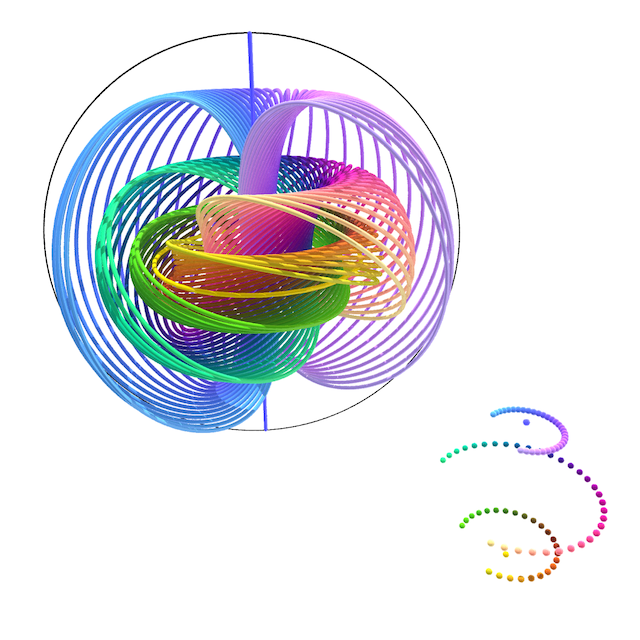
\includegraphics[scale=0.2]{Images/Hopf.png}
        \captionof{figure}{Hopf fibration in stereographic projection, i.e.\ as a fibration of $\bbR^3$. Each circle is a fiber corresponding to a point on the 2-sphere at the bottom. From \cite{hopf}.}
        \label{Fig.Hopf}
    \end{minipage}
\end{example}

\begin{xca}
    Show that in the Hopf bundle, the pre-image of any circle in $\bbS^2$ is a two-torus $\bbT^2$ embedded into $\bbS^3$.
\end{xca}


\begin{defn}[Bundle morphism]\index{Bundle morphism}
    Let $E\overset{\pi}{\to}M$ and $E'\overset{\pi'}{\to}M'$ be two smooth \glspl{fb}. A bundle morphism (a.k.a.\ \emph{bundle map}) between them is a pair of smooth maps $\wt{h}:E\to E'$ and $h:M\to M'$ such that $\wt{h}$ ``covers'' $h$ in the sense that the following square commutes:
    \[\begin{tikzcd}[every matrix/.append style={name=m},   
    execute at end picture={\draw [<-] ([xshift=-8mm,yshift=1mm]m-2-2.north) arc[start angle=-90,delta angle=270,radius=0.25cm];}]
       E \arrow[r,"\wt{h}"]\arrow[d,swap,"\pi"]& E'\arrow[d,"\pi'"] \\
       M\arrow[r,swap,"h"]& M'
    \end{tikzcd}\]
    This gives rise to the category $\FB^\infty$ of all smooth \glspl{fb}. A full subcategory is the category $\FB^\infty_M$ of all smooth \glspl{fb} over a given base $M$ with $h=\id_M$ (note that in general there are other bundle morphisms between bundles over $M$ for which $h$ is not even a diffeomorphism). Bundle morphisms covering the identity are also called \emph{vertical}.
\end{defn}








\subsection{Structure groups}\label{sec: structure groups}

So far we have only given a purely topological (or geometric in the smooth case) description of fiber bundles. The fascinating thing about fiber bundles, however, is that the requirement of local triviality gives rise to an alternative \emph{algebraic} description of fiber bundles, which will eventually lead us into the realm of cohomology. A similar, but more cumbersome, description appears for general topological fibrations as well. We now characterize fiber bundles in terms of their systems of local trivializations and identify their transition maps with certain Lie group actions. Note that everything here easily translates to the category of topological fiber bundles as well.


\begin{defn}[Bundle atlas, $G$-structure, cocycle]
    Let $E\overset{\pi}{\to}M$ be a smooth \gls{fb} with typical fiber $F$, and let $\{U_\alpha\}_\alpha$ be an open covering of $M$ such that the restrictions $\restr{E}{U_\alpha}$ are trivial. By definition of local triviality, we have some diffeomorphisms $\chi_\alpha: \restr{E}{U_\alpha}\to U_\alpha\times F$, called \emph{local trivializations}. Then:
\begin{itemize}

    \item The collection $\{(U_\alpha,\chi_\alpha)\}$ is called a \emph{\gls{fb} atlas} for $E\overset{\pi}{\to}M$. Two bundle atlases are \emph{equivalent} if their union is still a bundle atlas. A \emph{bundle structure} on $E$ is an equivalence class of bundle atlases, or, alternatively, a \emph{maximal atlas} given by the union of all atlases belonging to an equivalence class.
    
    \item For any point $(m,f)\in U_{\alpha\beta}\times F$, the transition maps in this atlas have the form \[\chi_\beta\circ\chi_\alpha^{-1} (m,f)=(m, t_{\beta\alpha}(m,f)),\label{eq transition functions}\], 
    where for every fixed $m\in M$, the map $t_{\beta\alpha}(m,\_):F\to F$ is a diffeomorphism. One can think of $t_{\beta\alpha}$ as a function on $U_{\alpha\beta}$ that takes values in the group $\Diff(F)$ of all diffeomorphisms of $F$, so $t_{\beta\alpha}$ becomes a map $t_{\beta\alpha}:U_{\alpha\beta}\to \Diff(F)$.\tablefootnote{As we will see in Section~\ref{sec: Diff groups}, the group $\Diff(F)$ can be given the structure of an infinite-dimensional Lie group, modeled on the space $\fX(F)$ of vector fields. Unfortunately $t_{\alpha\beta}$ are not always automatically smooth: they are smooth iff their values are contained in the left coset of the open and closed subgroup $\Diff_c(F)$ of diffeomorphisms with compact support. This is in principle true only for bundles which are ``trivial near fiber-wise infinity'' or have ``discrete structure group near diberwise infinity'' (see P.W.~Michor ``Gauge theory for diffeomorphism groups'', 1988). We shall always assume that this is true.}
    These $\Diff(F)$-valued functions are called \emph{bundle transition functions}. They are also sometimes called \emph{clutching functions}, especially when $M$ is a sphere.\index{Clutching functions}\index{Transition functions} We will usually assume that $\Diff(F)$ acts on the typical fiber from the \emph{left} (one can pass to a right action by acting via $t_{\alpha\beta}^{-1}$ instead).
    
    \item If the bundle structure of $E$ contains a bundle atlas whose transition functions take values in a Lie subgroup $G<\Diff(F)$,\tablefootnote{We will formalize the concept of Lie subgroups in Section\ref{sec: Lie theory iii}. For now all we need to know is that Lie subgroups are weakly embedded, which means that restricting a smooth map into $\Diff(F)$ whose image lies in $G<\Diff(F)$ in its range produces a smooth map into $G$. In fact, all subgroups of a Lie group are Lie subgroups.} then such an atlas is called a \emph{$G$-atlas} for $E$. Two $G$-atlases are called \emph{$G$-equivalent} if their union is still a $G$-atlas. A $G$-equivalence class of $G$-atlases, or, alternatively, the maximal $G$-atlas equal to their union, is called a \emph{$G$-structure}, denoted $\calG$.\index{$G$-structure} If a $G$-structure is fixed on $E$, we say that $G$ is the \emph{structure group} of the bundle. \index{Structure group} The tuple $(E\overset{\pi}{\to}M,G\acts F,\calG)$ is called a \emph{$G$-bundle}.\index{$G$-bundle}
    
    \item If $H<G$ is a Lie subgroup and a given $G$-structure on $E$ contains an $H$-atlas, then a choice of an $H$-structure (which is a subset of the given $G$-structure) is called a \emph{reduction of the structure group}, or simply a \emph{bundle reduction}\index{Bundle reduction} from $G$ to $H$.
    
    \item From the definition (\ref{eq transition functions}) it is obvious that the group-valued bundle transition functions satisfy two important conditions:
    \[
    \begin{cases}
    t_{\alpha\alpha}\equiv e, & \text{(identity condition),}\\
    \restr{t_{\alpha\beta}\cdot t_{\beta\gamma}\cdot t_{\gamma\alpha}}{U_{\alpha\beta\gamma}}\equiv e; & \text{(cocycle condition),}
    \end{cases}
    \]
    where the product in $\Diff(F)$ is just the composition of maps. Any collection of such $G$-valued functions $\{t_{\alpha\beta}\}$ associated to an open covering of $M$ is called a \emph{cocycle}\index{Cocycle} on $M$ with structure group $G$.\tablefootnote{More precisely, a cocycle is a certain equivalence class of such collections, which is discussed below.} Note that these two conditions imply $t_{\alpha\beta}t_{\beta\alpha}=e$.
\end{itemize}
\end{defn}

\begin{rem}\label{rem: faithful action on F 0}
    \begin{enumerate}
        \item One can try writing down higher-order relations on the transition functions, such as $t_{\alpha\beta}t_{\beta\gamma}t_{\gamma\delta}t_{\delta\alpha}=e$, but all of them follow from the identity and the cocycle conditions. Meanwhile, replacing the cocycle condition with only $t_{\alpha\beta}t_{\beta\gamma}=e$ would've been insufficient because this doesn't imply the higher-order relations.
        \item $\Diff(F)$ acts on $F$ faithfully by definition, therefore the induced action of any subgroup $G<\Diff(F)$ is faithful as well. This is why in the following definitions we will assume a priori that the action of the structure group on the model fiber is faithful. We will further elucidate the importance of faithfulness in Remark~\ref{rem: faithfulness of action on F}.
        \item A fiber bundle $E\to M$ is trivial iff it admits an $\{e\}$-structure. Indeed, if there is a bundle atlas in which all transition functions evaluate to the identity, then all local trivializations agree on the overlaps and hence stitch into a global trivialization.
    \end{enumerate}
\end{rem}


Since the structure group of a bundle acts on its typical fiber $F$, that is, it acts in the local trivializations, it is natural to ask whether this action ``lifts'' to an action on the actual fibers of the bundle itself. Crucially, the answer is no, however the following restricted concept of a $G$-structure does get naturally translated to the fibers.

\begin{defn}[$G$-fiber]
    Let $F$ be a smooth manifold diffeomorphic to a given manifold $F_0$ and let $G$ be a Lie group acting faithfully from the left on $F_0$, so $G$ can be identified with a Lie subgroup of $\Diff(F_0)$. Two diffeomorphisms $\chi_1,\chi_2:F\to F_0$ are called $G$-equivalent if $\chi_2\circ \chi_1^{-1}\in G$. A $G$-equivalence class $\calG_0$ of such diffeomorphisms, i.e.~an orbit of the action of $G$ on $\Diff(F,F_0)$ by compositions $\chi\mapsto g\circ \chi$, is called a fiber $G$-structure on $F$.\tablefootnote{This terminology is not standard. Unfortunately by a $G$-structure on a manifold people usually mean a $G$-structure on its tangent bundle, whereas our definition here refers to a $G$-structure on the bundle consisting of one fiber over a single point, $F\overset{\pi}{\to}\ast$.} The tuple $(F,G\acts F_0,\calG_0)$ is called a $G$-fiber modeled on $F_0$. An element of $\calG_0$ is called a \emph{$G$-frame}, or a frame \emph{compatible} with the $G$-structure.
\end{defn}


\begin{prop}
    If $\pi:E\to M$ is a fiber bundle with structure group $G$ acting on the typical fiber $F$, then each fiber of $E$ naturally carries a fiber $G$-structure and an action of the center $Z(G)$.
\end{prop}
\begin{proof}
    Consider a fiber $E_m=\pi^{-1}(m)$, $m\in M$. The fact that it carries a fiber $G$-structure is obvious because the value of any $G$-valued transition function at a point $m$ is an element of $G$. 
    
    We now show that if $G$ is not abelian, then there is no natural action of $G$ on the fibers, but there is an action of $Z(G)$. By definition of the typical fiber, there is a diffeomorphism $f_\alpha=\restr{\chi_\alpha}{E_m}:E_m\to F$, which is just the restriction of a local trivialization $\chi_\alpha$. By definition of a $G$-structure, there is a smooth (say left) action of $G$ on the typical fiber $F$. Let $f_\beta:E_m\to F$ be the diffeomorphism coming analogously from another compatible local chart. Then $f_\alpha(p)=t^{-1}\cdot f_\beta(p)$ for all $p\in E_m$ for some $t\in G$, and we can compare what the action of an element $g\in G$ translates to in the fiber $E_m$ under these two diffeomorphisms:
    \[f_\alpha^{-1}(g\cdot f_\alpha(p))=f_\beta^{-1}(tgt^{-1} f_\beta(p)).\]
    Since $t$ can range over all of $G$ by varying the charts, these formulas consistently define an action $g\cdot p$ only for $g\in Z(G)$.
\end{proof}

\begin{rem}
    \begin{enumerate}
        \item The intuition behind the definition of $G$-structures is the following. A fiber $G$-structure on $F$ is a choice of a $G$-invariant subset of all diffeomorphisms from $F$ to a ``standard'' or ``model'' space $F_0$, namely an orbit of the action of $G$ on all such diffeomorphisms by compositions. This can be interpreted as $F_0$ having some kind of ``structure'' that is invariant under actions of $G$, and a fiber $G$-structure allows us to transplant this structure to $F$. A $G$-structure on a fiber bundle, then, is a collection of structures on each fiber that, in a sense, vary smoothly with the base point $m\in M$. These structures are defined consistently because all local trivializations belonging to the same $G$-bundle atlas differ from each other by an action of $G$ on $F_0$, hence this additional structure is independent of the local bundle chart. 
        \item Morphisms between bundles with the same structure group are also defined so as to ``respect'' this structure. Thus the smaller the $G$, the more structure the morphisms of this category preserve. We will use this rough idea when introducing vector bundles, orientations, and complex bundles. For example, vector bundles will have group structure $\GL(V)$ for some vector space $V$, and, as we will see, the corresponding fiber $G$-structure is the structure of vector space.
        
        \item There is one extremely special class of $G$-bundles that will be distinguished by the fact that their typical fiber supports \emph{two} commuting actions of $G$, a left one and a right one (because the typical fiber will be $G$ itself). After using one of them up to define the bundle, we will be able to use the above procedure to lift the other one to a global action of $G$ on $E$. These bundles are called \emph{principal}. In Section~\ref{sec: free proper actions} we will show that principal $G$-bundles can be defined without reference to local trivializations, and in Section~\ref{sec: principal bundles} that will lead us to a chart-free definition of \emph{all} fiber bundles.
    \end{enumerate}
\end{rem}
\begin{example}
    A covering space $E\overset{\pi}{\to} M$ is a topological fiber bundle with a discrete typical fiber $F$. Its structure group, most generally, is the group $G=\Diff(F)=\mathrm{Bij}(F)$ of all permutations of points of the fiber. As we know, there is a natural $\pi_1(M,x_0)$-action on $F=\pi^{-1}(x_0)$, which produces a homomorphism $\lambda:\pi_1(M,x_0)\to G$. Note that there is no natural action of $\pi_1(M,x_0)$ on \emph{other} fibers of $E$ because there is no natural way to choose the isomorphisms between the groups $\pi_1(M,x_0)$ for different choices of the basepoint $x_0$. The image of $\lambda$ is a subgroup of $G$. Since the covering space can be fully reconstructed from this action, $\lambda(\pi_1(M,x_0))$ can be made the structure group of this bundle. 
    
    One case where there is a global action of the structure group on the whole covering space is when it is a $G$-principal covering space. In this case the fiber is $G$ itself and supports a second (right) action of $G$ which survives the fiber bundle construction.
\end{example}






\subsection{Fiber morphisms}

Now we examine morphisms (and in particular isomorphisms) between bundles with different structures on them. General bundle morphisms are allowed to be arbitrary smooth maps when restricted to a single fiber, so we will need to find a special subclass of bundle morphisms that ``respects'' given structures in some way. Let us first look at the simpler case of a single fiber. Say we have a $G$-fiber $(F,G\acts F_0,\calG_0)$ and a $G'$-fiber $(F',G'\acts F_0',\calG_0')$. Then any map $h:F\to F'$ can be represented by a map $\wh{h}:F_0\to F_0'$ by using any two diffeomorphisms $\chi\in\calG_0\subset \Diff(F,F_0)$ and $\chi'\in\calG_0'\subset \Diff(F',F_0')$ as follows:
\[\wh{h}=\chi'\circ h\circ \chi^{-1}.\label{eq g-fiber f-hat}\]
Different choices of $\chi$ and $\chi'$ are equivalent to replacing $\wh{h}$ in this formula with $g'\circ \wh{h}\circ g^{-1}$ for some $(g,g')\in G\times G'$. Therefore we notice the importance of the action of the product group $G\times G'$ on the set $C^\infty(F_0,F_0')$ by compositions:
\[G\times G'\acts C^\infty(F_0,F_0'):\quad ((g,g'),\wh{h})\mapsto g'\circ \wh{h}\circ g^{-1}.\label{eq gg' action}\] 
A choice of a class of morphisms $\wt h$ then corresponds to a choice of a set of orbits of this action. For this we either need $F_0$ and $F_0'$ to carry additional structure (vector spaces, metric spaces, etc.) that provides such a choice in a canonical way, or to just specify the choice manually. If want to make these choices consistently across all possible pairs of model spaces $(F_0,F_0')$, this amounts to forming a category. We detail these methods below:
\begin{enumerate}
    \item Let $\calS$ be a subcategory of the category $\mathsf{Man}^\infty$ of smooth manifolds (it need not include neither all objects nor all morphisms). Then if the model spaces $F_0$ and $F_0'$ are objects of $\calS$, we denote
    \[\calS(F_0,F_0')=\mor_\calS(F_0,F_0').\]
    We think of the category $\calS$ as describing ``additional structure'' on the model spaces. We now define morphisms from $(F,G\acts F_0,\calG_0)$ to $(F',G'\acts F_0',\calG_0')$ as maps $h:F\to F'$ which, under some (and therefore any) diffeomorphisms $\chi\in\calG_0$ and $\chi'\in\calG_0'$, are represented by maps $\wh{h}:F_0\to F_0'$ belonging to $(G\times G')\cdot \calS(F_0,F_0')$.
    
    \item In the situation of item 1, it is also often the case that $G$ and $G'$ \emph{act by automorphisms}, i.e.\ by elements of $\Aut_\calS(F_0)$ and $\Aut_\calS(F_0')$, respectively. Then 
    \[(G\times G')\cdot \calS(F_0,F_0')=\calS(F_0,F_0').\]
    This situation comes with an extra benefit. Since $G$ preserves the additional structure on $F_0$, this structure can be ``lifted'' via any $\chi\in \calG_0$ so that $F$ itself naturally becomes an object of $\calS$. Thus, in addition to the action of $Z(G)$, the fiber will inherit some additional structure from the $G$-invariant structure on the model fiber. We will soon see how this works explicitly on the example of vector bundles.
    \item The most common setting is a special sub-case of 2, whereby $G$ and $G'$ are \emph{defined} as the groups of automorphisms of $F_0$ and $F_0'$, respectively, so we don't even need to specify them separately:
    \[G=\Aut_\calS(F_0),\quad G'=\Aut_\calS(F_0').\]
    The actions of $G$ and $G'$ in this case are given canonically, and we can proceed as in 1. In particular, this implies that every representative $\wh{h}$ of every \emph{automorphism} (invertible morphism of a $G$-fiber to itself) $h$ is an element of $G$.
\end{enumerate}

\begin{defn}[Category of $\calS$-fibers]\label{def S-fibers}
    Given a $G$-fiber $(F,G\acts F_0,\calG_0)$, a $G'$-fiber $(F',G'\acts F_0',\calG_0')$, and a subset $\calS(F_0,F_0')\subset C^\infty(F_0,F_0')$ determined from a category $\calS$ in one of the ways described above, a morphism between them is a smooth map $h: F\to F'$ such that its representative $\wh{h}$ defined by (\ref{eq g-fiber f-hat}) using any $\chi\in\calG_0$ and $\chi'\in\calG_0'$ belongs to the orbit of an element of $\calS(F_0,F_0')$ under the action (\ref{eq gg' action}) of $G\times G'$ on $C^\infty(F_0,F_0')$. We say that $h$ \emph{is modeled on} an element of $\calS(F,F')$. We call this category $\calS\mathsf{-Man}^\infty$ and its objects $\calS$-fibers. Note that $\calS$ is not enough to define this category -- one also needs to specify groups $G$ and their actions (unless $G=\Aut(F_0)$ as in case 3 above).

    In particular, two $G$-fibers $(F,G\acts F_0,\calG_0)$ and $(F',F\acts F_0,\calG_0')$ with the same structure group $G$ and model space $F_0$ are isomorphic if and only if there exists a diffeomorphism $h:F\to F'$ such that the map $\calG_0'\to \calG_0$ given by the composition $\chi'\mapsto h^\ast \chi'=\chi'\circ h$ is a bijection. If $G=\Aut_\calS(F_0)$, then this is equivalent to $\wh{h}\in G$ for all representatives (\ref{eq g-fiber f-hat}) of $h$.
\end{defn}

Note that the choice of the category $\calS$ for a given type of structure is not unique. In fact we mostly need this definition to produce a unique notion of \emph{isomorphism} of $\calS$-fibers and later $\calS$-bundles, whereas we won't really care what the rest of the morphisms look like. We now consider a number of important examples of $\calS$-fiber structures.
\begin{example}[Linear $G$-structures]
    \begin{enumerate}
        \item If $\calS=\mathsf{FinVect}_\bbK$ (finite-dimensional $\bbK$-vector spaces), then we get the category of $\mathsf{FinVect}_\bbK$-fibers with linear maps. Here, if the model space is $V$, then we define $G=\Aut_\calS(V)=\GL(V)$. A $G$-structure $\calG_0$ on $F$ is an equivalence class of diffeomorphisms $F\to V$ that differ by an automorphism of $V$. Since $V$ is a vector space, we can use any of these diffeomorphisms $\chi\in\calG_0$ to induce a vector space structure on $F$ itself: for $\lambda_1,\lambda_2\in\bbK$ and $e_1,e_2\in F$ we define the linear combination
        \[\lambda_1e_1+\lambda_2 e_2\coloneqq \chi^{-1}(\lambda_1\chi(e_1)+\lambda_2\chi(e_2)).\]
        This is well-defined because different $\chi$'s differ by a linear automorphism of $V$. In particular, this defines an action of scalar matrices $\lambda I$, $\lambda\in\bbK$, on $F$, which coincides with the induced natural action of the center $Z(G)$. Note that $\GL(V)$ has no natural action on $F$ because there is no natural isomorphism between $F$ and $V$! Thus the category $\calS\mathsf{-Fib}$ is isomorphic to $\calS$ itself.

        In fact, one can replace the category $\mathsf{FinVect}_\bbK$ with its skeleton $\mathsf{Sk}(\mathsf{FinVect}_\bbK)$, whose objects are \emph{standard} spaces $\bbK^n$, $n=0,1,\ldots$, and the only nontrivial morphisms are inclusions-as or projections-onto the first $n$ components. Indeed, every linear map between vector spaces is represented by one of these standard maps in some appropriately chosen bases. In this case an element of $\calG_0$, i.e.\ a \emph{frame}, determines a basis on $F$ and outputs the components of vectors in that basis.
        
        \item In general, if structure groups $G$ are defined as the automorphism groups $\Aut(F_0)$, then the resulting category $\calS\mathsf{-Fib}$ is equivalent to $\calS$ itself. This allows one to define many classical structures on vector spaces in terms of a countable set of ``standard'' ones. This shows the importance of allowing $G$ to not necessarily act by automorphisms. We proceed in this manner in the next several examples.
        
        \item If $\bbK=\bbR,\bbC,\bbH$, then we can let $\calS$ be the category of finite-dimensional vector spaces with a $\bbK$-valued dot product, or its skeleton consisting of spaces $\bbK^n$ with the standard dot product $\sum_{i=1}^n \wb{x}_i y_i$. For each model space $\bbK^n$ we also take its isometry group $G$, which is $\Or_n,\U_n$, or $\Sp_n$, respectively. Then $\calS$-fibers are vector spaces $F$ with a $G$-structure which allows us to lift the dot product onto $F$. There is a bijective correspondence between $G$-structures and dot products on $F$, so  $\calS\mathsf{-Fib}$ is exactly the category of vector spaces with a dot product and all linear maps. $G$-frames in this context are just orthonormal bases. We can also replace $\calS$ with the category of vector spaces $V$ with a dot product and linear morphisms whose operator norm is at most $1$ (this forces isomorphisms to be isometries), and letting $G=\Aut_\calS(V)$. Then $\calS\mathsf{-Fib}$ has the same objects but fewer morphisms.

        \item If we let $\calS=\mathsf{FinVect}_\bbK$ but redefine the structure group $G$ of a model space $V$ as $G=\GL^+(V)$, i.e.\ orientation-preserving automorphisms, then $\calS$-fibers are oriented vector spaces with linear maps between them. 

        \item If $\calS$ is again the category of standard real vector spaces $\bbR^n$, $n=0,1,\ldots$, and the structure group of $\bbR^n$ is $\SL_n(\bbR)$, then $\calS$-fibers are vector spaces with a volume form (a totally antisymmetric multilinear form of maximum rank) with linear maps between them. Alternatively we can let $\calS$ consist of $\bbR^n$'s with the standard volume form $\mathsf{v}_n$ and linear maps $f:\bbK^n\to \bbK^m$ such that $f^\ast \mathsf{v}_m=\lambda \mathsf{v}_n$ with $\lambda\in (-1,1]$ (this forces automorphisms to have determinant $1$), and define $G=\Aut_\calS(\bbR^n)\cong \SL_n(\bbR)$. Note that a volume form induces an orientation because $\SL_n(\bbR)\subset \GL_n^+(\bbR)$.

        \item Taking standard model spaces $\bbK^n$ with $G$ defined as the group that leaves the subspace $\bbK^p$ spanned by the first $p$ standard basis vectors, and linear maps that map the first $p$ directions of one space to the first $p$ directions of the other (not necessarily surjectively), we get the category $\calS\mathsf{-Fib}$ of vector spaces with ``$p$-directions''. It is isomorphic to the category of pairs $(V,W)$ where $W$ is a $p$-dimensional subspace of $V$, and morphisms are required to be maps of pairs (i.e.\ $W$ is mapped inside $W'$). Note that morphisms between standard spaces $\bbR^n\to \bbR^m$ are represented by matrices with the top right $p\times(n-p)$ block filled with zeroes (unless $p>m$, in which case it's just the right $m\times (n-p)$ block).

        \item Consider all free actions of the group $G=\GL_n(\bbZ)$ on $n$-dimensional vector spaces $V$. This means that $G$ is the group of linear automorphisms of $V$ that preserve some rank-$n$ lattice $\Lambda$ spanning $V$ (i.e.\ $\Lambda=\bbZ v_1+\cdots +\bbZ v_n$ for some basis $v_1,\ldots,v_n$). Then $\calS\mathsf{-Fib}$ is the category of vector spaces with an \emph{integral affine structure}. It is isomorphic to the category of pairs $(V,\Lambda)$ and linear maps mapping lattice to lattice.

        \item $\calS$ be the category of even-dimensional real vector spaces $V$ with a linear isomorphism $\sfJ:V\to V$ such that $\sfJ^2=-\id_V$ and linear maps $h:(V,\sfJ)\to(V',\sfJ')$ such that $h\circ \sfJ=\sfJ'\circ h$. Each $\sfJ$ defines a complex structure on $V$ by $\rmi v\coloneqq\sfJ(v)$. Then $G=\Aut_\calS(V)$ consists of matrices $A\in\GL(V)$ such that $\sfJ A=A\sfJ$ and is isomorphic to $\GL_n(\bbC)$ (exercise). $\calS\mathsf{-Fib}$ is isomorphic to $\calS$ itself and is the category of complex structures on real vector spaces with complex-linear maps between them. $\calS$ can also be replaced with its skeleton, which consists of standard complex structures on $\bbR^{2n}$:
        \[\sfJ_{2n}=\begin{bmatrix}
            0&-I_n\\
            I_n&0
        \end{bmatrix}\]
        And linear maps $f:\bbR^{2n}\to \bbR^{2m}$ that satisfy $\sfJ_{2m}\circ f=f\circ \sfJ_{2n}$. In the case $m=n$ such maps are called holomorphic and their matrices have the form 
        \[M=\begin{bmatrix}
            A&B\\
            -B&A
        \end{bmatrix},\label{eq complex matrices}\]
        which can be identified with $A+\rmi B\in \Mat_n(\bbC)$.
        Note that each complex structure also induces an orientation because matrices $A\in \GL_n(\bbC)\subset \GL_{2n}(\bbR)$ have positive determinant over $\bbR$, namely $\det M=|\det(A+\rmi B)|^2>0$.

        \item Consider standard spaces $\bbR^{2n}$ with standard symplectic forms, i.e.\ antisymmetric nondegenrate bilinear forms $\omega_{2n}:\bbR^{2n}\times \bbR^{2n}\to \bbR$ whose matrix in the standard basis is $\sfJ_{2n}$. Let morphisms be all linear maps and let $G=\Sp_{2n}(\bbR)$ be the group of symplectic matrices, i.e.\ matrices $A\in\GL_{2n}(\bbR)$ such that $A^T\sfJ_{2n}A=\sfJ_{2n}$. Then $\calS$-fibers are symplectic vector spaces $(V,\omega)$ with all linear maps between them. This can be reduced to just the category of \emph{symplectomorphisms}, i.e.\ isomorphisms that preserve the symplectic structure.
    \end{enumerate}
\end{example}


\begin{example}[Hermitian structures]
    A Hermitian structure on a complex vector space $V_\bbC$ is just a symmetric sesquilinear form $\sfh:V_\bbC\times V_\bbC\to \bbC$ as introduced in example 2, i.e.
    \[h(v,w)=\widebar{h(w,v)},\quad v,w\in V_\bbC,\]
    and $h(v,v)\geq 0$ for all $v\in V_\bbC$ and vanishes iff $v=0$.
    
    An $n$-dimensional complex vector space is naturally isomorphic to a $2n$-dimensional real vector space with a complex structure $V_\bbC\cong (V,\sfJ)$ (defined by $\sfJ(v)\coloneqq \rmi v$), also denoted $V_\sfJ$. Then $\sfh$ can be reinterpreted as a complex-valued $\bbR$-bilinear form on $V_\sfJ$ which in addition satisfies
    \[\sfh(v,\sfJ w)=-\sfh(\sfJ v,w)=\rmi\sfh(v,w),\quad v,w\in V_\sfJ,\]
    and such that $\sfh(v,v)$ is a norm. This also implies that
    \[\sfh(\sfJ v,\sfJ w)=\sfh(v,w).\]
    We can decompose $\sfh$ into its real and imaginary parts, which we suggestively call $\sfg$ and $\omega$:
    \[\sfh(v,w)=\Re \sfh(v,w)+\rmi\Im\sfh(v,w)=\sfg(v,w)+\rmi \omega(v,w).\]
    We have
    \[\sfg(v,w)=\Re \sfh(v,w)=\Re \sfh(w,v)=\sfg(w,v),\]
    and $\sfg(v,v)=\sfh(v,v)$, therefore $\sfg$ is a nondegenerate symmetric bilinear form that defines a dot product on $V_\sfJ$.
    Furthermore, the sesquilinear condition implies that 
    $\omega(v,w)=\frac12 (\rmi\sfh(w,v)-\rmi\sfh(v,w))=\frac12 (\sfh(w,\sfJ v)-\sfh(v,\sfJ w))$
    is a real antisymmetric bilinear form. 
    Moreover,
    \[\omega(v,\sfJ w)=\frac12 (\sfh(\sfJ w,\sfJ v)+\sfh(v,w))=\frac12 (\sfh(w,v)+\sfh(v,w))=\Re \sfh(v,w)=\sfg(v,w),\]
    therefore $\omega$ is nondegenerate as well, and hence determines a symplectic structure on $V_\sfJ$. 

    Crucially, fixing a complex structure $\sfJ$, the above formulas relating any two of the three objects $\sfh,\sfg,\omega$ uniquely determine the third. We thus have natural isomorphisms between the following three pairs of structures:
    \begin{enumerate}
        \item Hermitian structures $(\sfJ,\sfh)$ on $V$.
        \item Pairs $(\sfJ,\sfg)$ of a complex structure $\sfJ$ and a metric $\sfg$ that are compatible in the sense that
        \[\sfg(\sfJ v,\sfJ w)=\sfg(v,w),\quad \text{or}\quad \sfg(\sfJ v,w)=-\sfg(v,\sfJ w),\quad v,w\in V.\]
        This compatibility condition is equivalent to the bilinear form $\omega_\sfJ(v,w)=\sfg(\sfJ v,w)$ being a symplectic form, also called the \emph{fundamental form}.
        \item Pairs $(\sfJ,\omega)$ of a complex structure $\sfJ$ and a symplectic structure $\omega$ that are compatible in the sense that
        \[\omega(\sfJ v,\sfJ w)=\omega(v,w),\quad \text{or}\quad \omega(\sfJ v,w)=-\omega(v,\sfJ w),\quad v,w\in V,\]
        and in addition that the resulting form $\sfg_\sfJ(v,w)=\omega(v,\sfJ w)$, which is symmetric because of compatibility, is positive definite (in this case we say that $J$ \emph{tames} $\omega$). These conditions are equivalent to the bilinear form $\sfg_\sfJ$ being a real scalar product.
        \item Pairs $(\sfg,\omega)$ of a positive definite metric $\sfg$ and a symplectic form $\omega$. By non-degeneracy of $\sfg$, there exists a unique operator $\sfJ$ such that $\omega(v,w)=\sfg(v,\sfJ w)$, and it follows that $\sfJ$ is a complex structure compatible with both $\sfg$ and $\omega$.
    \end{enumerate}
    Thus the group of isometries of $\sfh$, $\U(V,\sfh)$, coincides with the following double intersections of groups $\Sp(V,\omega)$ (automorphisms preserving $\omega$), $\GL(V_\bbC)$ (automorphisms preserving $\sfJ$), and $\Or(V,\sfg)$ (automorphisms preserving $\sfg$):
    \[\U(V,\sfh)=\Sp(V,\omega)\cap \GL(V_\bbC)=\Or(V,\sfg)\cap \GL(V_\bbC)=\Or(V,\sfg)\cap \Sp(V,\omega).\]
    In particular, for standard model spaces $(\bbR^{2n},\sfJ_{2n})$ we get the \emph{``2 out of 3 property of unitary groups''}:
    \[\U_n=\Sp_n(\bbR)\cap \GL_n(\bbC)=\Or_{2n}\cap \GL_n(\bbC)=\Or_{2n}\cap \Sp_n(\bbR),\]
    which is also obvious from the fact that any two of the defining equations $A^T\sfJ A=\sfJ$, $A^{-1}\sfJ A= \sfJ$, $A^TA=I$, imply the third.
    Here, $\GL_n(\bbC)$ is included in $\GL_{2n}(\bbR)$ as the set of invertible matrices of the form (\ref{eq complex matrices}) identified with $A+\rmi B\in \GL_n(\bbC)$.
    
    The triple $(\sfJ,\sfg,\omega)$ consisting of compatible complex, metric, and symplectic structures on $V$ can be called a \emph{linear K\"ahler structure}.\index{K\"ahler structure} As we have seen, the set of K\"ahler structure is bijective with the set of Hermitian structures, which is why in the linear case the term K\"ahler structure is redundant.
\end{example}

\begin{xca}
    \begin{enumerate}
        \item Show that the space of metrics on a vector space is convex, i.e.\ for any two metrics $\sfg_1$ and $\sfg_2$, all bilinear forms $t\sfg_1+(1-t)\sfg_2$, $t\in[0,1]$, are also metrics. Hence it is contractible.
        \item Show that the space of Hermitian forms $\sfh$ is also convex and hence contractible.
        \item Show that the set $\calJ(V,\omega)\subset \GL(V)$ of complex structures compatible with a given symplectic form $\omega$ (but not necessarily taming it) is contractible. See \cite[Prop.~7.5.7]{RS1}.
    \end{enumerate}
\end{xca}







\subsection{Bundle morphisms}

Now we extend our definition of morphisms to arbitrary \glspl{fb}. Consider a morphism $\wt{h}:E\to E'$ between two arbitrary bundles $E\overset{\pi}{\to}M$ and $E'\overset{\pi'}{\to}M'$ with potentially differing structure groups $G$ and $G'$. Pick local trivializations $\{(U_\alpha,\chi_\alpha)\}_{\alpha\in A}$, $\{(U_a',\chi_a')\}_{a\in A'}$ on the two bundles with corresponding cocycles $\{t_{\alpha\beta}\}$ and $\{t_{ab}'\}$ and denote $U_{\alpha a}=U_\alpha\cap h^{-1}(U_a')$. Then the bundle morphism is locally represented by maps
$\wh{h}_{\alpha a}:U_{\alpha a}\times F\to F'$ as follows: 
\[\boxed{\wt{h}\left(\chi_\alpha^{-1}(m,f)\right)=\chi_a^{\prime-1}\left(h(m),\wh{h}_{\alpha a}(m,f)\right).}\label{eq def of hab}\]
By transforming to other local charts $\chi_\beta$ and $\chi_b'$ via formula (\ref{eq transition functions}) we have
\[\wt{h}\left(\chi_\beta^{-1}(m,t_{\beta\alpha}(m)\cdot f)\right)=\chi_b^{\prime-1}\left(h(m),t_{ba}'(h(m))\cdot\wh{h}_{\alpha a}(m,f)\right).\]
On the other hand, (\ref{eq def of hab}) written for $\wh{h}_{\beta b}$ implies
\[\wt{h}\left(\chi_\beta^{-1}(m,t_{\beta\alpha}(m)\cdot f)\right)=\chi_b^{\prime-1}\left(h(m),\wh{h}_{\beta b}\left(m,t_{\beta\alpha}(m)\cdot f\right)\right).\]
By comparing the right hand sides of the last two formulas and using the fact that $\chi_b'$ is a fiberwise diffeomorphism, we conclude that
\[\boxed{\wh{h}_{\beta b}\left(m,t_{\beta\alpha}(m)\cdot f\right)=t_{ba}'(h(m))\cdot \wh{h}_{\alpha a}(m,f).}\label{eq transformation of hab}.\]
This is a complicated condition on the collection of maps $\{\wh{h}_{\alpha a}\}$ with respect two different cocycles. Despite this condition these maps can still look like completely arbitrary smooth maps when restricted to a single fiber. However, in many cases we would like to consider only those bundle morphisms which, in some sense, respect the given group structures. To this end, consider the set of smooth maps $C^\infty(F,F')$ (which is an infinite-dimensional smooth manifold) and the left action of $G\times G'$ on it by compositions:
\[(G\times G')\acts C^\infty(F,F'):\quad ((g,g'),\varphi)\mapsto g'\circ \varphi\circ g^{-1}.\]
Then every $\hat{h}_{\alpha a}:U_{\alpha a}\times F\to F'$ can be used to define a fiberwise $G\times G'$-equivariant map
\begin{gather}
    \Phi_{\alpha a}: U_{\alpha a}\times (G\times G')\to C^\infty(F,F'),\\
    (m,(g,g'))\mapsto \left(f\mapsto g'\cdot \hat{h}_{\alpha a}\left(h(m),g^{-1}\cdot f\right)\right).\label{def Phiab}
\end{gather}
It is easy to see that this map is $G\times G'$-equivariant (with $G\times G'$ acting on itself from the left). Moreover, every fiberwise $G\times G'$-equivariant map arises this way ($\hat{h}_{\alpha a}$ can be recovered by substituting $g=g'=e$), although the correspondence of course is not bijective.\tablefootnote{Note how the fact that $\Phi_{\alpha a}$ are defined on sets of the form $U_{\alpha a}\times (G\times G')$ hints that they themselves represent a function defined globally on some fiber bundle with typical fiber $G\times G'$. We will return to this in our discussion of principal bundles.} The transformation rule (\ref{eq transformation of hab}) now becomes
\[\boxed{\Phi_{\beta b}(m,g,g')=\Phi_{\alpha a}\left(m,gt_{\beta\alpha}(m),g't_{ba}'(h(m))\right).}\label{eq transformation of Phiab}\]
We would like to put some restriction on the values of these maps in $C^\infty(F,F')$ that produces a well-defined class of bundle morphisms $\wt h$ which can be interpreted as ``respecting'' the given $G$- and $G'$-structures. This can be easily done by analogy with how we interpreted the structure of a $G$-fiber:
\begin{gather}
    \text{All maps }\{\Phi_{\alpha a}\}_{\alpha\in A,a\in A'}\text{ should be required to take values}\\
    \text{in a single orbit of the }G\times G'\text{-action on }C^\infty(F,F').
\end{gather}
This is a well-defined constraint because, due to the equivariance of $\Phi_{\alpha a}$, the transformation law (\ref{eq transformation of Phiab}) implies that the fiber above $p$ gets mapped to the same orbit regardless of the values of the indices $\alpha,a$.

\begin{defn}[Category ${\calS \mFB}^\infty$]\label{def S-bundle}
    Let the objects of the category $\calS\mFB^\infty$, called $\calS$-bundles, be all possible structured bundles $(E\overset{\pi}{\to}M,G\acts F,\calG)$ with model fibers $F\in\ob(\calS)$ and with sets of maps $\calS(F,F')\subset C^\infty(F,F')$ determined from a category $\calS$. Morphisms from such a bundle to another one, $(E'\overset{\pi'}{\to}M',G'\acts F',\calG')$, are bundle morphisms $\wt{h}:E\to E'$ such that $\calG$ and $\calG'$ contain some $G$- and $G'$-atlas, respectively, in which $\wt{h}$ is represented by a collection of $G\times G'$-equivariant maps $\{\Phi_{\alpha a}\}$ as above which satisfy the compatibility condition (\ref{eq transformation of Phiab}) and which take values in the orbit of a single element of $\calS(F,F')$ under the action of $G\times G'$ on the set $C^\infty(F,F')$. We say that $\wt{h}$ \emph{is modeled on} an element of $\calS(F,F')$.

    In addition, ${\calS\mFB}_M^\infty$ is the subcategory of structured bundles over the fixed base manifold $M$ with morphisms covering the identity in $M$, i.e.\ we assume $h=\id_M$.
\end{defn}

There are a number of other subcategories one may define by additionally either fixing the fiber, the structure group, or both. The most important subcategory for us will be the following.

\begin{defn}[Category $\FB^\sigma$]\label{def FB^sigma}
    The category $\FB^\sigma$ consists of so called $(G,\sigma)$-bundles with a fixed structure group $G$, typical fiber $F$, and faithful action $\sigma:G\times F\to F$. The morphisms are required to be such that their local representatives lie in the orbit of the identity map on $F$. That is, locally morphisms are represented simply by actions of elements of $G$ on $F$.
\end{defn}


\begin{example}
    Consider the cylinder $E=\bbS^1\times\bbR $ as a line bundle over the circle. We can trivialize it with all transition functions being the identity. In the category of all line bundles (with structure group $\Diff(\bbR )$) there is a bundle map $E\to E$ that maps $(p,x)\mapsto (p,-x)$. However, in the category of bundles with the trivial structure group $G=\{e\}$ (i.e.\ the category of trivial bundles) this is not an allowed bundle map because it does not act trivially on the fiber.
\end{example}


\begin{defn}[Bundle construction]\label{def bundle construction}
    \Glspl{fb} can be alternatively defined by specifying the base manifold $M$, the typical fiber $F$, the structure group $G$ acting on the fiber via a \emph{faithful}\tablefootnote{The importance of faithfulness will be explained in Remark~\ref{rem: faithfulness of action on F}.} smooth left action which can be viewed as an injective homomorphism of Lie groups $\Phi:G\to \Diff(F)$ (i.e.\ we will write $g\cdot f=\Phi(g)(f)=\Phi_g(p)$ for $g\in G, f\in F$), a countable open covering $\{U_\alpha\}$ of $M$, and a cocycle  $t_{\beta\alpha}\in C^\infty (U_{\alpha\beta}, G)$. Namely, we can define $E$ as a topological space as the quotient $E\coloneqq \bigslant{(\bigsqcup_\alpha U_\alpha \times F)}{\sim}$, where $(m_1,f_1)\sim(m_2,f_2)$ iff $m_1=m_2=m$ and $f_1=t_{\beta\alpha}(m,f_2)$ for some $\alpha,\beta$, and the projection $\pi$ is defined as the descendent of the projections onto the fist component in each summand.\tablefootnote{In categorical terms, this is literally the cofibered product (pushout) of the sets $U_\alpha \times F$ with pairs of maps $\restr{\chi_\alpha^{-1}}{U_{\alpha\beta}\times F}$ and $\restr{\chi_\beta^{-1}}{U_{\alpha\beta}\times F}$. For instance, if there were only two sets $U_1,U_2$, we would have $E=(U_1\times F)\sqcup_Z (U_2\times F)$, where $Z=U_{12}\times F$ and we have two morphisms $\restr{\chi_i^{-1}}{U_{12}\times F}:Z\to U_i\times F$ that are used in the definition of the pushout.}
    Then $E$ has a unique smooth structure that makes $\pi$ a smooth submersion (see \cite[Lem.~10.6]{Lee} for the case of vector bundles, which is easily generalized to all \glspl{fb}).\tablefootnote{Essentially we can take an atlas $\{F_\alpha,\psi_\alpha\}$ of $F$ and an atlas $\varphi_\alpha$ of $M$ (\gls{wlog} subordinate to the covering $\{U_\alpha\}$) to construct a smooth atlas $\{(U_\alpha\times F_\beta,\varphi_\alpha\times\psi_\beta)\}$ of $E$.} This construction is called the \emph{clutching construction} of a \gls{fb}.
\end{defn}


The fact that any $(G,\sigma)$-bundle over $M$ can be uniquely reconstructed from a $G$-valued cocycle on $M$ means that this category doesn't really depend on the fiber $F$ and the action $\sigma$ very much. Namely, for any other faithful $G$-action $\sigma':G\times F'\to F'$ there is an equivalence of categories
\[C_{\sigma',\sigma}:\FB^\sigma\to \FB^{\sigma'}.\]
The functors going in either direction take a bundle, choose a cocycle for it, and then construct the other bundle using the same cocycle via the other action. Faithfulness of the actions is clearly necessary for this to be an equivalence of categories because only then are the cocycles uniquely defined. The key insight flowing from this equivalence is that, to study arbitrary fiber bundles, it will suffice to pick one particular kind of typical fibers and group actions on them which makes computations easy. This computationally convenient class of bundles turns out to be the class of \emph{principal bundles}, where the typical fiber coincides with the structure group. We discuss them in the examples below.



\begin{example}[Linear $G$-structures on manifolds]
    \begin{enumerate}
        \item Regardless of $\calS$, if $G=\{e\}$, then a $G=\{e\}$-structure is equivalent to a global trivialization of the bundle. In the case of vector bundles, this is called an \emph{absolute parallelism}.\index{Parallelism!absolute}
        \item $\calS=\mathsf{FinVect}_\bbR$, and the structure group of each vector space $F$ is $\GL(V)$, then $\calS$-bundles are just vector bundles. Each fiber is naturally an $\calS$-fiber, i.e.\ a vector space, and vector bundle morphisms are exacly fiberwise linear bundle morphisms.
        \item A $\GL_k^+$-structure on a vector bundle of rank $k$ is called an orientation because it selects an orientation on every fiber in a continuous fashion. A vector bundle that admits such a structure is called \emph{orientable}.\index{Orientable vector bundle}
        \item An $\Or_k$-structure on a vector bundle $E$ of rank $k$ is equivalent to a smooth choice of metrics $\sfg_m$ on each fiber $E_m$. In Section~\ref{sec: Riemannian mfds} we will see that every real manifold admits such a choice, called a \emph{Riemannian structure}, so every vector bundle admits a (non-unique) reduction of the structure group to an orthogonal group. $\Or_k$-bundles are known as \emph{Riemannian bundles}. This fact is equivalent to the statement that $\GL_k(\bbR)$ deformation retracts onto $\Or_n$. In addition, if the bundle is orientable, the structure group can be reduced to $\SO_n$.
        \item A $\GL_k(\bbC)$-structure on a real vector bundle $E$ of rank $2k$ is equivalent to a smooth choice of complex structures $\sfJ_m$ on each fiber $E_m$. Such bundles are called \emph{complex vector bundles} of rank $k$. Every complex vector bundle is oriented.
        \item A $\Sp_{2k}(\bbR)$-structure on a (real) vector bundle $E$ of rank $2k$ is equivalent to a smooth choice of symplectic forms $\omega_m$ on each fiber $E_m$. If such a choice exists, we get a \emph{symplectic vector bundle}.
        \item A $\U_k(\bbR)$-structure on a rank $k$ complex vector bundle is a smooth choice of a Hermitian dot product on each fiber. As we will see, every complex vector bundle admits such a choice, thus any $\GL_k(\bbC)$-structure can be reduced to a $\U_k$-structure. Note that a further reduction to $\SU_k$ is not always possible, and its existence doesn't have a standard name (we will later see that it is equivalent to the triviality of the determinant line bundle $\det E$, or to the vanishing of the first Chern class, $c_1(E)=0$).
    \end{enumerate}
    Note that every one of these structures, just like in the linear case, defines a canonical choice of frames (bases) in each fiber, and via local trivializations they can be chosen smoothly over an open subset of the base. 
\end{example}

\begin{example}[Nonlinear $G$-bundles]
    \begin{enumerate}
        \item If $\calS=\mathsf{LieGr}$ with the structure group of each Lie group $G$ being its automorphism group $\Aut(G)$, then $\calS$-bundles are what is called \emph{group bundles}. Since automorphisms preserve the identity and the rest of the group structure, each fiber of a group bundle carries a natural Lie group structure. In particular, each group bundle has one canonical section $\sigma_e:M\to E$ whose value in each fiber is the identity element of that fiber.\index{Group bundle}
        
        \item If $\calS=\mathsf{LieGr}$ but with the structure group of a Lie group $G$ being $G$ itself acting by left translations, then we get what are called \emph{principal bundles} and they are so important that we shall put off a detailed discussion of them until Section~\ref{sec: principal bundles}. For now we only note the crucial difference between group and principal bundles: the fibers of a principal $G$-bundle, despite being diffeomorphic to $G$, are not Lie groups since left translations don't preserve the identity element.\index{Principal fiber bundle} This is another important example where the group action on the typical fiber falls outside of the set of morphisms allowed by the category $\calS$.
    \end{enumerate}
\end{example}

The following theorem is one of the most important theorems for the applications of fiber bundle theory, for example in complex-analytic problems of differential equations (where it is known as the Riemann-Hilbert factorization problem).

\begin{thm}\label{bundle isomorphism thm}
Two $G$-bundles $E$ and $E'$ over $M$ are isomorphic iff there exists a covering $\{U_\alpha \}$ of $M$, two corresponding cocycles $\{t_{\alpha\beta}\}$ and $\{t_{\alpha\beta}'\}$, and a set of $G$-valued functions $\lambda_\alpha:U_\alpha\to G$ such that $t_{\alpha\beta}'(p)\equiv \lambda_\alpha (p) t_{\alpha\beta}(p) \lambda_\beta^{-1}(p)$ for all $p\in U_{\alpha\beta}$. In particular, a bundle is trivial iff its transition functions can be factorized as $t_{\alpha\beta}=\lambda_\alpha \lambda_\beta^{-1}$.
\end{thm}
\begin{proof}
Given two bundle atlases over $M$, we can always take all possible pairwise intersections of the sets of the two covers of $M$ to refine the atlases so that they are defined over the same covering of $M$. \gls{wlog}, any isomorphism of bundles over the same base can be assumed be identity on the base itself (e.g. because if the horizontal part of the isomorphism is some diffeo $f:M\to M$, we can replace one of the bundles by the isomorphic pullback bundle along $f$, see Definition~\ref{Pullback bundle}). Then from (\ref{eq transformation of hab}) we see that any bundle isomophism gives rise to the $\lambda_\alpha$'s, and vice versa, $\lambda_\alpha$'s completely describe the bundle isomorphism. 
\end{proof}
\begin{defn}[Equivalent cocycles]
    Two $G$-valued cocycles on $M$ that are related (after being brought over to a common set of charts $\{U_\alpha\}$) by the above formulas for some collection of maps $\lambda_\alpha:U_\alpha\to G$ are called \emph{$G$-equivalent}. The equivalence class $[\{t_{\beta\alpha}\}]$ itself is also called a cocycle.
\end{defn}
\begin{cor}
    Given a manifold $M$ and a faithful smooth action $G\overset{\sigma}{\acts} F$, there is a bijective correspondence between isomorphism classes of $(G,\sigma)$-bundles over $M$ and ($G$-equivalence classes of) $G$-valued cocycles on $M$.
\end{cor}
This correspondence can actually be restated as an equivalence of the category $\FB^\sigma$ and a certain category of cocycles.

\begin{rem}\label{rem: faithfulness of action on F}
    Faithfulness of the action is crucial here. As we noted in Remark~\ref{rem: faithful action on F 0}, any structure group whose action is induced from the action of $\Diff(F)$ acts on $F$ faithfully. We can see the importance of this property when recostructing a bundle from a cocycle acting on a model fiber. If, for example, $F$ is a single point, then every group action on $F$ is trivial and there is only one fiber bundle over $M$ with fiber $F$ regardless of the structure group $G$, whereas there are still many non-equivalent $G$-valued cocycles on $M$. Therefore faithfulness is needed so that the cocycle is well-defined in this sense. In the future we will run into important situation where, for instance, $F$ is a finite-dimensional vector space with an action of a non-linear group $G$ (namely a spin group), so that this action cannot be faithful, and thus the correspondence with classes of cocycles will not be one-to-one.
\end{rem}






\subsection{Flat bundles}

Now let us try to use this transformation rule for transition functions to ``simplify'' the cocycle and see how far we can go. If we have two charts with a transition function $t_{\alpha\beta}$, then we always find a pair of functions $\lambda_\alpha,\lambda_\beta$ on those charts such that $\lambda_\alpha t_{\alpha\beta}\lambda_\beta^{-1}$ is constant, in fact equal to identity: just pick $\lambda_\alpha=e$ and let $\lambda_\beta$ be an arbitrary smooth extension of $t_{\alpha\beta}$ from $U_{\alpha\beta}$ to all of $U_\beta$. We can try to keep expanding this procedure to more and more charts, but there is no guarantee that we will be able to make all transition functions constant. Thus we single out the following important class of bundles.

\begin{defn}[Flat $G$-structure]\index{Flat!fiber bundle}\index{Flat!$G$-structure}
	A $G$-structure on a \gls{fb} is called \emph{flat} if it contains a bundle atlas with constant (or locally constant) transition functions. Alternatively, a $G$-structure is flat if structure group $G$ can be reduced to a subgroup with a \emph{totally disconnected} topology (one where all connected subsets are one-point sets, e.g.\ the discrete topology; then the transition functions are forced to be constant by continuity). If the default $\Diff(F)$-structure is flat, then the bundle itself is called flat.
\end{defn}
\begin{rem}
    Note that the flatness of the bundle (with respect to the default $\Diff(F)$-structure) does not imply that all other $G$-structures on it are flat.
\end{rem}


\begin{example}[Line bundles above $\bbS^1$]\label{line bundles over S1}
    We can use the idea of a bundle atlas and Theorem \ref{bundle isomorphism thm} to classify all line bundles above the circle up to isomorphisms. It suffices to pick one covering of the circle, so we will pick a covering by the three circular arcs $U_1=(\epsilon,4\pi/3-\epsilon)$, $U_2=(2\pi/3+\epsilon,2\pi-\epsilon)$, and $U_3=(4\pi/3+\epsilon,8\pi/3-\epsilon)$. The transition functions in a line bundle take values in the group $G$ of diffeomorphisms of $\bbR $. Each such diffeomorphism is a smooth function $f:\bbR \to\bbR $ such that $f'$ is never zero. Now, clearly $G$ consists of two path-connected components, one of diffeomorphisms that preserve the orientation, i.e.\ $f'(x)>0$ for all $x$, and others that reverse it, $f'(x)<0$. We say that these diffeomorphisms have one of two possible \emph{parities}. Let $g_+(x)=\id_{\bbR }(x)=x$ and $g_-(x)=-x$, so that $g_+$ is the identity element of $\Diff(\bbR )$ and $g_-$ is an orientation-reversing involution.

    There are three transition functions, $t_{12}$, $t_{23}$, and $t_{31}$. Any three $G$-valued functions $\lambda_1,\lambda_2,\lambda_3$ provide an isomorphic line bundle. Choose $\lambda_1\equiv g_+$. Furthermore, $t_{12}:U_{12}\to G$ can be extended to a continuous function $\lambda_2: U_2\to G$, $\restr{\lambda_2}{U_{12}}=t_{12}$. Then $t_{12}'=\lambda_1 t_{12}\lambda_2^{-1}\equiv g_+$. By continuity, all values of $\lambda_2$ have the same parity.  Now, we let $\lambda_3$ be a continuous extension to $U_3$ of the function $\lambda_2 t_{23}:U_{23}\to G$. Then $t_{23}'=\lambda_2 t_{23} \lambda_3^{-1}\equiv g_+$. Finally, $t_{31}'=\lambda_3 t_{31} \lambda_1=\lambda_3 t_{31}$.  The parity of the values of $t_{31}'$ by construction is the product of the parities of $t_{12}$, $t_{23}$, and $t_{31}$.

    The values of $\lambda_3$ are already uniquely fixed up to the point $2\pi-\epsilon=-\epsilon$. Due to the path-connectedness of the two components of $G$, $\lambda_3$ can be deformed on $U_3\setminus U_{23}=(-\epsilon,2\pi/3-\epsilon)$ so that it remains smooth and $\restr{\lambda_3}{(\epsilon,2\pi/3-\epsilon)}=g_\pm t_{31}^{-1}$, which leads to $t_{31}'\equiv g_\pm$.

    This means that any line bundle above $\bbS^1$ is isomorphic to one of two bundles, whose transition functions are either all identities, or one of them is a reflection $x\mapsto -x$.  In other words, any line bundle over $\bbS^1$ can be reduced to the structure group $O(1)=\bbZ_2$. The former bundle is trivial, and the latter bundle is homeomorphic to the M\"obius band. There are only two isomorphism classes of line bundles above $\bbS^1$.
\end{example}

\begin{xca}\label{Rk-bundles above circle}
    Show that if $f:\bbR^K\to \bbR^k$ is a diffeomorphism such that $f(0)=0$, then $f_t(x)=f(tx)/t$ is a homotopy from $f$ to an element of $\GL_k(\bbR)$. Use this to argue that the group $\Diff(\bbR^k)$ has only two path-connected components, and that there are only two isomorphism classes of \glspl{fb} with fiber $\bbR^k$  above $\bbS^1$ for any $k$.
\end{xca}
\begin{xca}
    Show that every diffeomorphism of the circle $\bbS^1\subset \bbC$ is homotopic to one of the two maps $z\mapsto z^{\pm 1}$. Using this fact, classify all circle bundles over $\bbS^1$ (i.e.~with typical fiber $\bbS^1$). Note that this result can also be obtained from Exercise~\ref{Rk-bundles above circle}.
\end{xca}

\begin{example}
    Staying in the category of topological fiber bundles, let us classify two-fold covering spaces of the ``figure eight space'' in the language of fiber bundles. The fiber $F$ in this case consists of two points. The base space $M=\bbS^1\vee \bbS^1$ can be covered by three contractible sets: one $\mathsf{x}$ and two intervals. All of their overlaps are contractible, and therefore by adjusting the transition functions we will always be able to make them constant. This we have four overlaps with four corresponding elements of the structure group $G=S_2$. The bundle will be constructed out of the disjoint union of two copies of each of our three pieces: we need to glue the following six pieces $\begin{matrix}
        |\; \times \;|\\
        |\; \times \;|
    \end{matrix}$. Now note that two of the transition functions, namely one on the left side of the base manifold $\infty$ and one on the right, can be turned into the identity by permuting the two pairs of straight segments to match those two permutations. Thus we end up with two copies of $\infty$, where each loop has been cut at one point, giving us two pairs of cuts to glue back using the two permutations. Since each permutation can only take two values, we get a total of four covering spaces. Two of them happen to be isomorphic if we allow for nontrivial diffeomorphisms of the base (the left-right symmetry of $\infty$), but usually the classification is done without considering such symmetries. One of the fiber bundles obtained this way is trivial, and the other three are represented in Figure \ref{fig:coverings of 8}(1,2).
\end{example}

\begin{example}[Covering spaces and flat bundles with flat connections]
	Covering spaces are just \glspl{fb} with discrete fibers, therefore their structure group $G$ is the permutation group of the points of the typical fiber. The classification theorem for covering spaces stated that all bundles over $M$ with the discrete fiber $F$ are classified by all possible homomorphisms $\pi_1(M)\to G$ (up to global conjugation by an element of $G$ corresponding to a shuffling of the points of $F$). Therefore, up to the fact that the action of $\pi_1(M)$ is often not faithful, we can say that the structure group of any covering space over $M$ is $\pi_1(M)$.
	
	Continuing Remark~\ref{covering spaces and connections}, we see that the monodromy, or holonomy, is also nothing but a representation of $\pi_1(M)$ on the fiber. Therefore bundles with discrete fibers are completely classified by the monodromy/holonomy of the connection on them. Can we generalize these ideas to a larger class of bundles?
	
	First of all, by a simple extension of the argument in Example \ref{line bundles over S1}, we see  that all bundles with fiber $F$ and structure group $G$ above $\bbS^1$ are classified by homomorphisms $\Hom(\pi_1(M),\pi_0(G))/\sim$, where $\pi_0(G)=G/G_0$ and $G_0$ is the connected component of the identity in $G$ (which is a normal subgroup), so that $\pi_0(G)$ is the group whose elements are the connected components of $G$. The equivalence relation is the global conjugation of all values of the given homomorphism by an arbitrary element of the target group (corresponds to a diffeomorphism on $F$, which of course doesn't change the bundle). For instance, for $F=\bbR $ and $G=\Diff(\bbR )$, we found that $\pi_0(G)=\bbZ_2$. The statement also agrees with the classification theorem for covering spaces.
	
	Recall that a connection is just a prescription for lifting curves from the base into the total space. The lifted curves are called \emph{horizontal}, and the lifting procedure is also known as \emph{parallel transport} (of the starting point in the bundle along the path in the base). If the curve in the base is a loop $\gamma$ such that $\gamma(0)=\gamma(1)=p\in M$, then its lifts with all possible starting points $\wt{\gamma}(0)=e_0\in E_p$ determine the holonomy $e_0\mapsto e_1=\wt{\gamma}(1)=h(\gamma)(e_0)$, where we introduced the map $h:\gamma\mapsto h(\gamma)\in G$. Defined this way, $h(\gamma)$ is an element of the structure group $G$, and moreover $h$ is a homomorphism from the group $L_p(M)$ of all loops based at $p$ to $G$. The image of this homomorphism is a subgroup $\mathrm{Hol}_p<G$ called the \emph{holonomy group} of the bundle based at $p$. If $h$ is restricted only to contractible loops, then the corresponding group is called $\widetilde{\mathrm{Hol}}_p<\mathrm{Hol}_p<G$, the \emph{local holonomy} group at $p$. 
	
	If $\widetilde{\mathrm{Hol}}_p=\{\id\}$ for all $p$, the connection is called \emph{flat}. This is equivalent to the property that the holonomy depends only on the homotopy class of the base loop. In particular, a small simply connected neighborhood $U\subset M$ of $p\in M$ can be uniquely lifted to a local section of $E$ passing through $e_0\in E_p$, which is of course diffeomorphic to $U$. That is, $E$ can be locally fibrated by horizontal sections, each diffeomorphic to $U$. 
	
	Flatness of a connection is sometimes called \emph{integrability}\index{Integrability}, and is exactly what people mean when they speak of integrable systems in physics: the phase space of an integrable system can be fibrated by hypersurfaces that are locally spanned by physical trajectories.
	
	Finally, we notice that the definition of flat \glspl{fb} given above implies the existence of a flat connection. Namely, a loop $\gamma$ in $M$ that passes through charts $U_1,U_2,\ldots,U_n=U_1$ with the starting point $(p,f)\in U_1\times F$ can be lifted as $(\gamma(t),f)$ on $U_1$, $(\gamma(t),\tau_{21}f)$ on $U_2$, $(\gamma(t),\tau_{32}\tau_{21}f)$ on $U_3$, and so on (here $\tau_{ij}\in G$ represent the constant transition functions). These actually stitch together into a continuous path under the identifications in the bundle. Similarly one can lift non-closed curves, which completes the definition of the connection.
	
	Exercise: check that the local holonomy of the connection just described is independent of the choice of a bundle atlas (even though the connection itself does depend on the atlas) and trivial , i.e.\ the connection is indeed flat.
	
	The non-local part of the holonomy is described by ordered products of transition functions $\prod \tau_{ij}$ along non-contractible loops. Since these are homotopy-invariant, we have a homomorphism $\pi_1(M)\to G$ that completely describes the holonomy of the flat connection. A global conjugation $g\mapsto g_0 g g_0^{-1}$ on the group doesn't affect the connection (it is essentially equivalent to shifting the base point in the definition of $\pi_1(M)$), therefore all flat connections on bundles with structure group $G$ above $M$ are classified by $\Hom(\pi_1(M),G)/\sim$, where $\sim$ is the conjugation equivalence. Moreover, one can show that every homomorphism of this kind corresponds to a bundle with a connection. This is the generalization of the classification theorem for covering spaces.
	
	Note that a flat bundle with structure group $G$ and a flat connection is the same as a fiber bundle whose structure group is $G$ with the discrete topology (because in the latter situation the transition functions as well as all deformation parameters $\lambda_\alpha$ are forced to be constant functions, the flat connection is unique and given by the construction above). All this leads us to conclude that flat bundles with a flat connection, or bundles with totally disconnected structure groups, are the natural generalization of covering spaces.
	
	We have shown that bundles over $M$ with a totally disconnected structure group $G$ are precisely classified by the conjugacy classes of homomorphisms $\Hom(\pi_1(M),G)$. The conjugacy class of such homomorphisms corresponding to a bundle $E\overset{\pi}{\to}M$ is called the \emph{characteristic class}\index{Characteristic class} of the bundle. Therefore, for totally disconnected structure groups, a single characteristic class determines the isomorphism class of the bundle.
	
	The main goal for Parts \ref{Part II} and \ref{Part III} of these lectures will be to develop the machinery necessary for the full classification of \glspl{fb} with arbitrary topological structure groups, in particular by extending the theory of characteristic classes. The characteristic class we have just constructed (acting on one-dimensional cycles, i.e.\ closed loops) is only the first one in an infinite list of cohomology classes corresponding to a given bundle.
\end{example}

\begin{comment}
    \begin{samepage}
        \PRLsep
        \begin{center}
            {\red Lecture 9 on 25 Jan 2019 ended here}
        \end{center}
    \end{samepage}
\end{comment}








\subsection{Subbundles, pullbacks}


We've seen that bundles are, in categorical terms, pushouts (i.e.\ quotients of disjoint unions) of a family of trivial bundles along the trivialization maps. The categorical notion of pullback introduced in Definition \ref{pullbacks} is also very useful in the theory of \glspl{fb}.

\begin{defn}[Pullback bundle]\index{Pullback bundle}\label{Pullback bundle}
    Let $E\overset{\pi}{\to}M$ be a smooth \gls{fb} and $N\overset{f}{\to}M$ a smooth map. We define the \emph{pullback of $E$ along $f$}, or the bundle \emph{induced from $E$ by $f$}, denoted $f^\ast E$, in three ways:
    \begin{itemize}        
        \item $f^\ast E=\{(n,p)\in N\times E\mid f(n)=\pi(p)\}\subset E\times N$ with the subspace topology induced from $E\times N$. Obviously we have two canonical projections onto the two components of the product, $f^\ast E\overset{\wt{f}}{\to}E$ and $f^\ast E\overset{\pi'}{\to}N$. The latter one is the new bundle projection, equal to the restriction of the natural projection $\pr_1$ on $N\times E$. We show below that there is a unique smooth structure on $f^\ast E$ that makes $\pi'$ into a smooth submersion.
        \item If the typical fiber of $E$ is $F$ and we know a set of transition functions $t_{\alpha\beta}:U_{\alpha\beta}\to G$ defining $E$, then $f^\ast E$ can be defined as the bundle with base $N$, same fiber $F$, and transition functions $f^\ast t_{\alpha\beta}:f^{-1}(U_{\alpha\beta})\to G$, where $f^\ast t\coloneqq t\circ f$ is the definition of the \emph{pullback of a function} $t$ on $M$ via $f$.
        \item In categorical terms, it is literally the pullback $N\times_M E$ that uses the maps $E\overset{\pi}{\to}M$ and $N\overset{f}{\to}M$ in its Cartesian square. This object indeed exists because it can be explicitly constructed using either of the next two alternative definitions. The pullback naturally comes with two canonical projections $f^\ast E\overset{\wt{f}}{\to}E$ and $f^\ast E\overset{\pi'}{\to}N$.
    \end{itemize} 
    \[\begin{tikzcd}[every matrix/.append style={name=m},   
    execute at end picture={\draw [<-] ([xshift=-8mm,yshift=1mm]m-2-2.north) arc[start angle=-90,delta angle=270,radius=0.25cm];}]
   f^\ast E \arrow[r,"\wt{f}"]\arrow[d,swap,"\pi'"]& E\arrow[d,"\pi"] \\
   N\arrow[r,swap,"f"]& M
    \end{tikzcd}\label{eq pullback bundle diagram}\]
\end{defn}

\begin{lem}[{{\cite[Prop.~1.7.3, Rem.~1.7.4]{RS1}}}]\label{prop 1.7.3 RS1}
    Let $N$ be a smooth manifold and $M\subset N$ a subset with the relative topology induced from $N$. Consider the following condition.
    \begin{enumerate}[label=(E)]
        \item \begin{enumerate}[label=(E\alph*)]
            \item $M\subset \bigcup_i V_i$,
            \item for every $i$, $V_i\cap M$ admits a smooth structure of dimension $l$ with respect to which it is an embedded submanifold of $N$.
        \end{enumerate}
    \end{enumerate}
    If condition (E) holds for some $l\in\bbN$, the smooth structures on $V_i\cap M$ induce a smooth structure on $M$, with respect to which $M$ is an embedded submanifold of $N$. Conversely, if there exists a smooth structure on $M$ which makes it an embedded submanifold of dimension $l$, then (E) holds for this $l$ and the induced smooth structure on $M$ coincides with the original one.
\end{lem}
\begin{proof}
    Pick local slice charts $(V_i,\rho_i)$ on $N$ such that $\rho(V_i\cap M)=\rho_i(V_i)\cap (\bbR^l\times \{0\})$. As a topological subspace of $N$, $M$ is Hausdorff and second countable. For every $i$, $V_i\cap M$ is open in the relative topology. Being the restriction of a homeomorphism onto its image, $\restr{\rho_i}{V_i\cap M}$ is a homeomorphism onto its image. Since by assumption the image is $\rho_i(V_i)\cap (\bbR^l\times\{0\})$ and is hence open in $\bbR^l\times\{0\}$, these data give a local chart on $M$. The transition maps are obtained by restriction of the original local charts on $N$ to subsets of the subspace $\bbR^l\times\{0\}$ which are open by condition (E2). Hence the transition maps are smooth and define a smooth structure. By definition of the relative topology the inclusion is open onto its image, thus $M$ is embedded.
\end{proof}


\begin{prop}[{{\cite[Prop.~2.6.1]{RS1}}}]\label{prop 2.6.1 RS1}
\begin{enumerate}
    \item $f^\ast E$ defined via any of the first two definitions has a unique smooth structure that turns the bundle projection into a smooth submersion.
    \item All three definitions are isomorphic as smooth bundles.
    \item $f^\ast E$, defined as in the first definition, is in fact an embedded submanifold of $N\times E$.
\end{enumerate} 
\end{prop}
\begin{proof}
    We apply Lemma~\ref{prop 1.7.3 RS1}. Choose a typical fiber $F$ and a system of local trivializations $\{(U_\alpha,\chi_\alpha)\}$ for $E$. For every $\alpha$ consider the open subset $V_\alpha=f^{-1}(U_\alpha)$ of $N$ and the mapping  
    \[\psi_\alpha:V_\alpha\times F\to N\times E,\quad \psi_\alpha(m,u)=(m,\chi_\alpha^{-1}(f(m),u)).\]
    Since $\psi_\alpha$ is obtained by composing the diffeomorphism $\chi_\alpha^{-1}$ with the natural inclusion mapping of the graph of $\restr{f}{V_\alpha}:V_\alpha\to U_\alpha$, it is a smooth embedding (see Example~\ref{example submanifolds}). Hence the image $\psi_\alpha(V_\alpha\times F)$ inherits a smooth structure from $V_\alpha\times F$ with respect to which it is an embedded submanifold of $N\times E$. Since the image is $f^\ast E\cap (V_\alpha\times\pi^{-1}(U_\alpha))$ and since the $V_\alpha\times\pi^{-1}(U_\alpha)$ are open subsets of $N\times E$ covering $f^\ast E$, we conclude that $f^\ast E$ is an embedded submanifold. This proves assertion 3, and Lemma~\ref{prop 1.7.3 RS1} also shows the uniqueness of this smooth structure, proving assertion 1. Assertion 2 is an exercise.
\end{proof}

\begin{xca}[Pullback of a bundle by itself]
    Given the $n$-fold covering of the circle $\bbS^1\overset{\pi}{\to}\bbS^1$, show that the pullback $\pi^\ast \bbS^1=\bbS^1\times_{\bbS^1} \bbS^1$ is a trivial fiber bundle over $\bbS^1$. As we will see later, this is a general fact about \emph{principal} fiber bundles.
\end{xca}

\begin{rem}
\begin{enumerate}
    \item From the proof of Proposition~\ref{prop 2.6.1 RS1}, every local trivialization of $E$ induces a local trivialization of $f^\ast E$. In particular, the pullback of a trivial bundle is trivial. As indicated above, transition functions also get simply pulled back by $f^\ast \tau_{\alpha\beta}=\tau_{\alpha\beta}\circ f$.
    \item A bundle morphism $H:E'\to E$ covering a map $h:M'\to M$ naturally decomposes as
    \[E'\overset{H_{\mathrm{ver}}}{\to} h^\ast E\overset{H_{\mathrm{hor}}}{\to} E,\label{eq 2.6.2 RS1}\]
    where $H_{\mathrm{ver}}(x)=(\pi'(x),H(x))$, $x\in E'$, and $H_{\mathrm{hor}}=\wt{h}$ is the induced vector bundle morphism $\wt{h}$ defined by the pullback diagram (\ref{eq pullback bundle diagram}). One can check that $H_{\mathrm{ver}}$ is a vertical bundle morphism and that $f^\ast E$ is an embedded submanifold of $N\times E$.  Using this decomposition, one can give the following characterization of isomorphisms in terms of their projections and fiber mappings: a bundle morphism is an isomorphism iff its projection (the map in the base) is a diffeomorphism and its fiber mappings are bijective.
\end{enumerate}
\end{rem}


\begin{defn}[Restriction of a bundle]\index{Restriction of a fiber bundle}
    If $S< M$ is a submanifold via an immersion $i:S\to M$ and $E\overset{\pi}{\to}M$ is a smooth \gls{fb}, then we can define the restricted bundle $\restr{E}{S}\coloneqq i^\ast E$. It is a smooth \gls{fb} by the last proposition.
\end{defn}

\begin{defn}[Spaces of sections]\index{Section of a fiber bundle}
    A smooth section of a smooth \gls{fb} $E\overset{\pi}{\to}M$ is a smooth map $\sigma:M\to E$ such that $\pi\circ \sigma=\id_M$. The space of all sections, with the compact-open topology, is denoted $\Gamma^\infty_M(E)$. If $U\subset M$ is an open subset, or more generally an immersed submanifold, then a \emph{local section} over $U$ is a section of the restricted bundle $\restr{E}{U}$, and the space of all local sections over $U$ is denoted $\Gamma^\infty_U(E)=\Gamma^\infty(\restr{E}{U})$.
\end{defn}
\begin{rem}
    It is not in general true that every local section can be realized as a restriction of a global section. For example, the two-fold cover of the circle $\bbS^1\to \bbS^1$ has no global sections at all. More broadly, the properties of bundles that prevent an extension of local structures to global ones are called \emph{obstructions}. The obstructions to the existence of global sections turn out to be of purely algebraic-topological nature and are described by cohomology, as we will see in Part~\ref{Part III}.
\end{rem}


\begin{xca}\label{example 2.7.3 RS1}
\begin{enumerate}
    \item Show that if $E$ is trivial, then $f^\ast E$ is trivial for any $f$. In other words, pullbacks of bundles are always ``at least as trivial'' as the original bundles.
    \item Show that if $(\wt{f},f)$ is a bundle map from $E$ to $E'$ that is also a fiberwise diffeomorphism, then $E\cong f^\ast E'$.
    \item Show that if $S<M$ is immersed, weakly embedded, or embedded, then $\restr{E}{S}$ is respectively an immersed, weakly embedded, or embedded, subbundle of $E$. See \cite[Example~2.7.3]{RS1}.
\end{enumerate}
\end{xca}



\begin{prop}
    Let $E\overset{\pi}{\to}M$ be a smooth \gls{fb} and let $\sigma:M\to E$ be a section (i.e.~a smooth map such that $\pi\circ\sigma=\id_M$). Then $(M,\sigma)$ is an embedded submanifold of $E$.
\end{prop}
\begin{proof}
    It suffices to show that there exists an open neighborhood $V$ of $\sigma(m)$ in $E$ such that $(\sigma^{-1}(V),\restr{\sigma}{\sigma^{-1}(V)})$ is an embedded submanifold. Since local trivializations are diffeomorphisms, this follows from the fact that the graph of any smooth map $\psi:M\to N$ is an embedded submanifold of $M\times N$.
\end{proof}



\begin{defn}[Fiber subbundle]\index{Fiber subbundle}
    A (immersed, weakly embedded, or embedded) subbundle of a smooth \gls{fb} $E\overset{\pi}{\to}M$ is a \gls{fb} $E'\overset{\pi'}{\to}M'$ with an injective \gls{fb} morphism $\wt{h}:E'\to E$ which turns $E'$ into an immersed, weakly embedded, or embedded, respectively, submanifold of $E$. If $M=M'$ then we usually assume that $\wt{h}$ covers the identity in the base, and we call such subbundles \emph{vertical}, or \emph{subbundles over $M$}. 
\end{defn}

\begin{prop}[{{\cite[Prop.~2.7.4]{RS1}}}]
    Consider a bundle morphism $H:E'\to E$ covering a map $h:M'\to M$.  \gls{tfae}:
    \begin{enumerate}
        \item $(E',H)$ is a subbundle (resp.~immersed, weakly embedded, embedded) of $E$.
        \item $(M',h)$ is a submanifold (resp.~immersed, weakly embedded, embedded) of $M$ and the fiber maps $H_m:E'_m\to E_m$ are injective for all $m\in M'$.
        \item In the decomposition (\ref{eq 2.6.2 RS1}), $(E',H_{\mathrm{ver}})$ is a vertical subbundle of $h^\ast E$ and $(h^\ast E,H_{\mathrm{hor}})$ is a subbundle (resp.~immersed, weakly embedded, embedded) of $E$.
    \end{enumerate}
\end{prop}
\begin{proof}
    $1\Rightarrow 2$ The fiber maps $H_m$ are obviously injective. Since Since all bundles have local sections, let $\sigma':U'\to E'$ be such a local section for $E'$. Then $H\circ\sigma'$ is a smooth local section over the set $h(U')$ (which may not be open) for $E$. Every local section over an open set is an embedding, in particular $\sigma'$, and thus its composition with another submanifold map, $H\circ \sigma'$, defines a submanifold of $E$ of the same type as $H$. This submanifold is the image of a section of $\pi$, and $\pi$ restricted to any section is a diffeomorphism onto the domain of that section. Thus the composition $\pi\circ H\circ \sigma':U'\to h(U')$ is also a submanifold of the same type. Finally, since $\pi$ is locally trivial, this means that every point $m\in M$ has a neighborhood $U$ such that $h(M')\cap U$ coincides with a submanifold of the form we described above. This implies that the entire image $h(M)$ is a submanifold.
    
    $2\Rightarrow 3$ Since the $H_m$ are injective, $H_{\mathrm{ver}}$ is injective, hence the assertion on $(E',H_{\mathrm{ver}})$ holds since every vertical subbundle is embedded. The assertion on $(h^\ast E,H_{\mathrm{hor}})$ was proven in Exercise~\ref{example 2.7.3 RS1}.

    $3\Rightarrow 1$ Since vertical subbundles are embedded, this follows from transitivity of submanifold properties as earlier in this proof.
\end{proof}




\subsection{Homotopy lifting property}


\begin{thm}[Bundles over $M\times I$ {{\cite[Thm.~3.3.1]{RS2}}}]\label{bundles over MxI}
    Every \gls{fb} $E$ over $M\times I$, where $I=[0,1]$, is isomorphic to $E_0\times I$ where $E_0=\restr{E}{M\times\{0\}}$. The isomorphism can be chosen so that its restriction to $E_0$ is the inclusion $E_0\hookrightarrow E\times I$ as $p_0\mapsto (p_0,0)$.
\end{thm}
\begin{proof}
    First we show that $E$ can be trivialized over a locally finite open covering of the form $\{U_i\times I\}_i$.

    By local triviality, for a fixed $x\in M$ and every $t\in I$, there is an open neighborhood $V_t\subset M$ of $x$ and an open interval $t\in I_t\subset I$ such that $E$ is trivial over $V_t\times I_t$. Therefore we can construct a countable, locally finite open covering of $M\times I$ with sets of this kind. By compactness, there is a finite set $0<t_1<\cdots<t_k<1$ such that $\bigcup_i I_{t_i}=I$. Let $V_i=V_{t_i}$, $I_i=I_{t_i}$, and define 
    \[
        U_i=\bigcap_{j=1}^i V_j,\quad J_i=\bigcup_{j=1}^i I_j.
    \]
    Obviously $E$ is trivial over $U_1\times J_1$. Let $\chi_1$ be a trivialization of $E$ over $U_1\times J_1$ and $\wt{\chi}_2$ -- one over $V_2\times I_2$. Then $(U_1\times J_1)\cap (V_2\times I_2)=U_2\times (J_1\cap I_2)$. Assuming that $I_2$ intersects $J_1$ non-trivially and one is not contained in the other (otherwise $I_2$ can be dropped from the covering of $I$), consider the transition function $\tau:U_2\times(J_1\cap I_2)\to G$ defined by $\chi_1(p)=\left(\id\times    \tau(\pi(p))\right)\cdot \wt{\chi}_2(p)$. Choose $c\in J_1\cap I_2$ and a continuous function $f:I_2\to J_1\cap I_2$ such that $f(t)=t$ for $t\geq c$ to define 
    \[
        \wt{\tau}:U_2\times I_2\to G,\quad \wt{\tau}(x,t)=\tau(x,f(t)).
    \]
    Clearly $\tau$ and $\wt{\tau}$ coincide on $U_2\times([0,c]\cap I_2)$. Hence the new mapping
    \[
    \chi_2(p)=\begin{cases}
    \chi_1(p), & \pi(p)\in U_2\times[0,c],\\
    (\id\times\wt{\tau}(\pi(p)))\cdot \wt{\chi}_2(p), & \pi(p)\in U_2\times I_2
    \end{cases}
    \]
    defines a trivialization of $E$ over $U_2\times I_2$. By induction, we find that $E$ is trivial over every every $U_i\times I$. 

    We sketch the rest of the proof. Since this construction applies to every $x\in M$, we can extract a locally finite open covering of the entire $M$ of the form $\{U_i\times I\}_i$ such that $E$ is trivial over every set in the covering (this can be done using a \gls{pou}). Let $\chi_i$ be the corresponding local trivializations and $\wh{\chi}_i$ the induced local trivializations of $\restr{E_0}{U_i}\times I$.

    Now we construct a global trivialization inductively in $i$. For $V_1=U_1$, there is already an isomorphism $\Phi_1:\restr{E}{V_1\times I}\to\restr{E_0}{V_1}\times I$. We can construct a chain of open sets $V_1\subset V_2\subset\cdots$ that eventually covers all of $M$ and $U_i\subset V_i$, and by induction extend the isomorphism to $\Phi_i:\restr{E}{V_i\times I}\to\restr{E_0}{V_i}\times I$. Via the local trivializations $\chi_i$ and $\wh{\chi}_i$, bundle isomorphisms are represented by $G$-valued functions $g_i:U_{i}\times I\to G$ with $g_i(x,0)=e\in G$. Let $g_1:(V_1\cap U_2)\times I\to G$ be the representative of $\Phi_1$ in $\chi_2$ and $\wh{\chi}_2$. Then $g_1$ can be smoothly extended to $V_2\times I$ so that it equals $e$ on $(U_2\setminus V_1)\times I$. This represents the isomorphism $\Phi_2$ that agrees with $\Phi_1$ on the common domain. Repeating this procedure on $U_3$ and so on, we construct a global isomorphism of the bundles in question. See \cite[Thm.~3.3.1]{RS2} for details.
\end{proof}

\begin{cor}
    Continuous deformations (homotopies) of transition functions within the class of cocycles don't change the isomorphism class of a fiber bundle.
\end{cor}



Therefore, in the most general and abstract sense, the ``full'' characteristic class\index{Characteristic class} of a fiber bundle (which uniquely classifies the bundle) is the ``conjugacy'' and homotopy equivalence class of cocycles for it.

Now we are ready to prove the smooth version of the \gls{hlp} for fiber bundles (a continuous version of it holds automatically since every smooth fiber bundle is a Hurewicz fibration).

\begin{thm}[Homotopy Lifting Property/Covering Homotopy Theorem]\label{HLP}
    Let $E\overset{\pi}{\to}M$ and $E'\overset{\pi'}{\to}M'$ be smooth \glspl{fb} with the same typical fiber $F$. If $(\wt{H}_0,H_0)$ is a bundle map from $E$ to $E'$ and $H:M\times I\to M'$ is a homotopy of $H_0$, i.e.\ $H_0=\restr{H}{M\times\{0\}}$, then there exists a bundle map $\wt{H}$ that covers $H$:
    \[\begin{tikzcd}[every matrix/.append style={name=m}, execute at end picture={\draw [<-] ([xshift=-9mm,yshift=1mm]m-2-2.north) arc[start angle=-90,delta angle=270,radius=0.2cm];}]
    E\times I \arrow[r,"\wt{H}"]\arrow[d,swap,"\pi\times\id"]& E'\arrow[d,"\pi'"] \\
    M\times I\arrow[r,swap,"H"]& M'
    \end{tikzcd}\]
\end{thm}
\begin{proof}
    Consider the map
    \[
    \lambda:E\to H_0^\ast E'\subset M\times E',\; \lambda(p)=(\pi(p),\wt{H}_0(p)).
    \]
    This is a bundle isomorphism of two bundles over $M$. Moreover, by Theorem \ref{bundles over MxI}, there exists a bundle isomorphism 
    \[
    \Phi:H^\ast E'\to \wt{H}_0^\ast E'\times I
    \]
    of bundles over $M\times I$ satisfying $\Phi\left((x,0),f\right)=\left((x,f),0\right)$. Together with the natural bundle morphism $\proj_2:H^\ast E'\to E'$, the isomorphisms $\lambda $ and $\Phi$ combine to a morphism
    \[
    \wt{H}:E\times I\overset{\lambda\times\id_I}{\longrightarrow}H_0^\ast E' \times I\overset{\Phi^{-1}}{\to}H^\ast E'\overset{\proj_2}{\to}E'
    \]
    that covers $H$. Since 
    \[
    \wt{H}(p,0)=\proj_2\circ\Phi^{-1}\left(\left(\pi(p),\wt{H}_0(p)\right),0\right)=\proj_2\circ \left(\left(\pi(p),0\right),\wt{H}_0(p)\right)=\wt{H}_0(p),
    \]
    $\wt{H}$ is indeed an extension of $\wt{H}_0$.
\end{proof}


% \begin{rem}
% The Path Lifting Property of covering spaces is a special case of the Homotopy Lifting Property when $M$ consists of one point, but with an extra uniqueness result that doesn't hold for general \glspl{fb}. In topology, fiber bundles (called Hurewicz fibrations, or the even more general Serre fibrations) are in fact defined through the Homotopy Lifting Property.
% \end{rem}


\begin{cor}\label{HLP cor}
\begin{enumerate}
    \item If $E'\overset{\pi'}{\to}M'$ is a \gls{fb} and $f,g:M\to M'$ are two smooth maps that are homotopic to each other, then the pullback bundles $f^\ast E'$ and $g^\ast E'$ are isomorphic.
    \item All \glspl{fb} over contractible base spaces are trivial.
\end{enumerate}
\end{cor}

\begin{proof}
\begin{enumerate}
    \item Let $H:M\times I\to M'$ be a homotopy from $f$ to $g$ and consider the bundle $P=H^\ast E'$ over $M\times I$. Let $P_t=\restr{P}{X\times\{t\}}$ viewed as a bundle over $M$. Then $P_0=f^\ast E'$ and $P_1=g^\ast E'$. By the above Theorem, $P$ is isomorphic to $P_0\times I$. By restricting the isomorphism to the subbundle $P_1\subset P$, we get an isomorphism from $P_1$ to $P_0$.
    \item Contractible spaces by definition are homotopy equivalent to a point, and all bundles over a point are trivial with the trivialization given by the pullback of the bundle bundle along the contraction.
\end{enumerate}
\end{proof}


We've established that fiber bundles are, roughly speaking, classified by homotopy-plus-conjugacy classes of cocycles. We now present the first elementary example in which this classification can be reduced to familiar algebraic objects.

\begin{cor}[Classification of fiber bundles over spheres]
     Isomorphism classes of \glspl{fb} over the sphere $\bbS^n$, $n\geq 1$, with fiber $F$ and a given faithful action $G\acts F$ of the structure group $G$ are in one-to-one correspondence with the homotopy classes of maps from $\bbS^{n-1}$ to the identity component $G_0$, up to conjugation by the discrete group of connected components of $G$, $G\slash G_0\cong \pi_0(G)$:
    \[
    \mathsf{Sk}\left(\FB_{\bbS^n}(G\acts F)\right)\cong [\bbS^{n-1},G_0]/\pi_0(G)= \pi_{n-1}(G)/\pi_0(G),\label{FB(G) and homotopy(G)}
    \]
    (here the group $\pi_0(G)$ acts on the set $\pi_{n-1}(G)$ by conjugation of the values, which is a well-defined action within homotopy classes). In particular, when $G$ is connected, this set forms a group isomorphic to $\pi_{n-1}(G)$.
\end{cor}
\begin{proof}
    We have already proven this for $n=1$ in Example~\ref{line bundles over S1}. For $n\geq 2$, $\bbS^n$ can be covered by two hemispheres $U_\pm$ that overlap along a neighborhood $U_0$ of the equator. The equator $C$ is diffeomorphic to $\bbS^{n-1}$ and $U_0$ can be chosen so that $U_0\cong \bbS^{n-1}\times (-1,1)$. Then the only transition function in any given bundle $E\overset{\pi}{\to}\bbS^n$ is $\tau:U_0\to G$. It can be chosen so that is maps a given point $x_0\in C$ to $e\in G$. Its restriction to the equator provides the \emph{clutching function}\index{Clutching function} $\theta=\restr{\tau}{C}:\bbS^{n-1}\to G_0$ whose homotopy class will be the one put into correspondence with the bundle. 
     
    To check that this mapping is consistent, we need to show that isomorphic bundles have homotopic clutching functions, up to conjugation by an element of $\pi_0(G)$. Let the two transition functions be $\tau_1$ and $\tau_2$ and consider an isomorphism given by $\tau_2=\lambda_+ \tau_1 \lambda_-^{-1}$, where $\lambda_\pm$ are two $G$-valued functions on $U_\pm$, respectively. Since $\tau_{1,2}(x_0)=e$, we can first consider the case when $\lambda_\pm(x_0)=e$ and therefore $\lambda_\pm$ take values in the connected component of the identity $G_0\subset G$. Then we can deform $\lambda_\pm$ by a homotopy so that $\lambda_+(P_+)=\lambda_-(P_-)=e\in G$, where $P_\pm$ are the respective poles of the sphere. Since $U_\pm $ are both diffeomorphic to a ball $B^n\in\bbR^n$, we can use the Cartesian coordinate $x$ on the ball to introduce the homotopy $\lambda_+(tx)\tau_1(x) \lambda_-^{-1}(tx)$ from $\tau_1$ to $\tau_2$. 
    
    Another choice for $\lambda_\pm$ is when $\lambda_+(x_0)=\lambda_-(x_0)=g_0$ with $g_0$ in another connected component of $G$ than the identity. Then the same argument leads to clutching functions that are, up to a homotopy, conjugates of each other by $g_0$. Different choices of $g_0$ within its connected component only change the clutching functions by a homotopy, just like above, because each connected component of $G$ is path-connected.
    
    Finally, the map constructed is clearly surjective because every function $\bbS^{n-1}\to G_0$ can be used to construct a fiber bundle. It is also injective because any two homotopic clutching functions $\theta_1\sim\theta_2:\bbS^{n-1}\to G$ can only be restrictions of two homotopic transition functions $\tau_1\sim\tau_2:\bbS^{n-1}\times(-1,1)\to G$ (all up to conjugation by $\pi_0(G)$). This is because every such $\tau(x,t)$ is homotopic to one that is independent of $t$ (and this is because every function on $(-1,1)$ is homotopic to a constant one).
\end{proof}


The above Corollary shows the importance of the computation of homotopy groups of at least the classical Lie groups. Interestingly, many of these groups can be computed \emph{using} certain fiber bundles. We will begin to do this in Section~\ref{sec: flag manifolds}.
\[\boxed{\begin{array}{c}
    \text{Our ultimate goal for Part \ref{Part III} will be to extend (\ref{FB(G) and homotopy(G)})}\\
    \text{to arbitrary base manifolds using the theory of characteristic classes.}
\end{array}}
\] 


\begin{example}[Vector bundles over $\bbS^1$]
    Now we can easily solve Exercise \ref{Rk-bundles above circle}. Consider only vector bundles of rank $k$ above $\bbS^1$. The structure group is $G=\GL_k(\bbR)$. This group has two connected components distinguished by the sign of the determinant. Therefore $\pi_0(G)=\bbZ_2$ and there are only two isoclasses of bundles. Equivalently we can classify bundles with a two-point fiber $\bbZ_2$ above $\bbS^1$. We have $G=\Diff(\bbZ_2)=\bbZ_2$ and
    \[
        \FB_{\bbS^1}(\bbZ_2)\cong \pi_{0}\left(\bbZ_2\right)=\bbZ_2.
    \]
    \end{example}
    \begin{example}[Plane bundles over $\bbS^2$]
    Let us classify all $\bbR^2$-bundles over $\bbS^2$. We have by Corollary \ref{HLP cor} that 
    \[
        \mathsf{Sk}\left(\FB_{\bbS^2}\left(\bbR^2\right)\right)\cong \pi_{1}\left(\GL_2(\bbR )\right)/\pi_0\left(\GL_2(\bbR )\right)=\bbZ/\bbZ_2\cong \bbZ
    \]
    Similarly we can classify circle bundles above the 2-sphere. The structure group of circle bundles is $\Diff(\bbS^1)$, which is homotopy equivalent to $\Or_2\cong \bbS^1\sqcup \bbS^1$. Therefore
    \[
        \mathsf{Sk}\left(\FB_{\bbS^2}\left(\bbS^1,\Or_2\right)\right)\cong \pi_{1}\left(\Or_2\right)/\pi_0\left(\Or_2\right)\cong\bbZ/\bbZ_2\cong\bbZ
    \]
    (because $\bbZ_2$ acts by conjugation, which is a trivial action on the abelian group $\bbZ$). If we were to restrict the structure group to orientation-preserving diffeomorphisms of the circle, we would need to replace $\Or_2$ by $\SO_2=\U_1$, so 
    \[
        \FB_{\bbS^2}(\bbS^1,\U_1)\cong \pi_{1}\left(\bbS^1\right)\cong\bbZ.
    \]
    This implies that every plane bundle over $\bbS^2$ is orientable. The integer number that classifies these (oriented) plane or circle bundles over the 2-sphere is called the \emph{Chern number}\index{Chern number} and represents yet another characteristic class of bundles.
\end{example}

\begin{example}[Hopf bundle revisited]\label{ex hopf bundle atlas}
    If we cover $\bbS^2$ by two disks $D_\pm$ overlapping along the equator, the Hopf fibration $\bbS^3\overset\pi\to \bbS^2$ (Example~\ref{Hopf bundle}) restricted to each of them is trivial and diffeomorphic to a solid torus in $\bbR^3$. Therefore the 3-sphere $\bbS^3$ can be broken up into two disjoint (aside from their boundary) solid tori that are glued to each other along the 2-torus that is their common boundary.The twists of the boundary performed in this process classify the resulting circle bundles over the 2-sphere, so here we will try to understand the case of the Hopf bundle. In terms of the coordinates on the bundle used in Example \ref{Hopf bundle}, we have 
    \[\restr{E}{D_+}=\{|z_1|\geq|z_2|\},\quad \restr{E}{D_-}=\{|z_1|\leq|z_2|\}.\]
    Note that $D_+=\bbS^2\setminus \{\pi(0,1)\}$ and $D_-=\bbS^2 P^1\setminus \{\pi(1,0)\}$. It is conventional to define $0\coloneqq \pi(1,0)$ and $\infty\coloneqq \pi(0,1)$. Therefore we can also call these sets $U_0\coloneqq D_+$ and $U_\infty\coloneqq D_-$. The standard complex coordinate on $U_0=D_+$ is $z\coloneqq \frac{z_2}{z_1}$ and on $U_\infty$, $w\coloneqq \frac{z_1}{z_2}$. The transition map is $w(z)=\frac{1}{z}$, which is complex analytic, so this atlas turns $\bbS^2$ into a \emph{complex manifold}, namely the projective complex line $\bbC P^1$.
    
    Over the equator $C$ we have 
    \[\restr{E}{C}=\left\{|z_1|^2=|z_2|^2=\frac12\right\},\]
    so the restriction of the Hopf bundle to the equator is a 2-torus with two angular coordinates $\varphi,\psi$, where $\varphi$ is the standard azimuthal coordinate on the sphere and $\psi$ is the coordinate in the fiber:
    \[\restr{E}{C}=\left\{(z_1,z_2)=\frac{1}{\sqrt{2}}\left(\rme^{\rmi\varphi/2+\rmi\psi},\rme^{-\rmi\varphi/2+\rmi\psi}\right)\right\}.\]
    Identifying $D_\pm$ with the unit disk $\mathbb{D}^2\subset\mathbb{C}$, we construct the bundle atlas
    \begin{align}
        \chi_0(z_1,z_2)=\left(\frac{z_2}{z_1},\frac{z_1}{|z_1|}\right)\in\mathbb{D}^2\times \bbS^1,\quad 0\leq|z_2|\leq |z_1|,\\
        \chi_\infty(z_1,z_2)=\left(\frac{z_1}{z_2},\frac{z_2}{|z_2|}\right)\in\mathbb{D}^2\times \bbS^1,\quad 0\leq|z_1|\leq|z_2|.
    \end{align}
    Incidentally, limiting $|z_1|$ and $|z_2|$ to $[0,\frac12]$, this shows once again that the 3-sphere is a union of two solid tori overlapping only at their common $\bbT^2$-boundary. Note that in this atlas, a point over the equator gets mapped to a conjugate pair of points on $\partial\bbD^2$ by $\pr_1\circ \chi_\pm$ (this could be fixed by redefining one of the charts, but that would violate the convenient analytic structure). These trivializations are indeed diffeomorphisms because their inverses are
    \begin{align}
        \chi_0^{-1}(z,\rme^{\rmi\psi})=\left(\frac{\rme^{\rmi\psi}}{{\sqrt{1+|z|^2}}},\frac{z\rme^{\rmi\psi}}{{\sqrt{1+|z|^2}}}\right),\quad (z,\rme^{\rmi\psi})\in \mathbb{D}^2\times \bbS^1,\\
        \chi_\infty^{-1}(z,\rme^{\rmi\psi})=\left(\frac{z\rme^{\rmi\psi}}{{\sqrt{1+|z|^2}}},\frac{\rme^{\rmi\psi}}{{\sqrt{1+|z|^2}}}\right),\quad (z,\rme^{\rmi\psi})\in \mathbb{D}^2\times \bbS^1.
    \end{align}
    We compute the clutching function
    \[\tau_{\infty0}(z)\cdot \rme^{\rmi\psi}=\pr_2\circ \chi_\infty\circ \chi_0^{-1}(z,\rme^{\rmi\psi})=\frac{z}{|z|}\cdot \rme^{\rmi\psi},\]
    in particular, on the equator, $\tau_{\infty0}(\rme^{\rmi\varphi})=\rme^{\rmi\varphi}$. Therefore, following a standard sign convention, the Chern number of this bundle equals $-1$.\tablefootnote{The sign of the Chern number is usually fixed by the complex structure of the corresponding bundle (which induces a specific orientation on the fibers). The Hopf bundle is the circle bundle of the complex line bundle $\calO(-1)$ defined over the Riemann sphere $\bbS^2=\mathbb{C}P^1$ as the complex line bundle with the transition function $\tau_{0\infty}(z)=z^{-1}$, and the Chern number of any holomorphic line bundle equals its degree, which in this case is $-1$. For the Hopf bundle itself, however, the sign of the Chern number is merely a convention.}
\end{example}


\begin{example}[Plane/circle bundles over $\bbS^2$ continued]\label{ex circle bundles over S2}
     \begin{enumerate}
        \item As we saw above, every plane bundle over $\bbS^2$ is orientable. This can be made more general. We will see later that non-orientability of a vector bundle over a manifold $M$ implies the existence of some nontrivial two-fold covering of $M$. Therefore every vector bundle over a simply connected base is orientable, since such manifolds have no non-trivial covering spaces.
        
        \item Since the transition functions of every circle bundle over $\bbS^2$ can always be reduced to $\U_1$, and $\U_1$ is abelian, every such bundle comes with a natural global free (and fiberwise transitive) action of $\U_1$. This bundle can be trivialized over two hemispheres, thus being decomposed into a gluing of two solid tori $\bbD^2\times \bbS^1$. Recall that the lens space $L(p;1)$ (Example~\ref{example Lens space bredon}) can similarly be decomposed into two solid tori glued along a map acting on the boundary torus $\bbT^2$ of one of them by $(\rme^{2\pi\rmi \varphi},\rme^{2\pi\rmi\psi})\mapsto (e^{2\pi\rmi\varphi},e^{2\pi\rmi(p\varphi+\psi)})$. But this is exactly the identification that produces the circle bundle over $\bbS^2$ with the transition function $\tau_{-+}(\rme^{2\pi\rmi\varphi})=\rme^{2\pi\rmi p\varphi}$. Thus the total space of every $\bbS^1$-bundle over $\bbS^2$ is a lens space. Note that $p=1$, corresponding to the Hopf bundle, gives the correct total space $L(1;1)=L(1;0)=\bbS^3$. Another example is $p=2$, which gives $\bbR P^3$. \index{Lens spaces}
    \end{enumerate}
\end{example}
   
\begin{rem}
    In the mid-20th century there was a conjecture that any two closed (compact with no boundary) manifolds of the same dimension that are homotopy equivalent must be homeomorphic. 3-dimensional lens spaces were the first counterexample: $L(p;q_1)$ and $L(p;q_2)$ are homotopy equivalent iff $q_1q_2\equiv \pm n^2\mod p$ for some $n\in\bbN$, but homeomorphic only if $q_1\equiv \pm q_2^{\pm 1}\mod p$.

    The enhanced conjecture of Armand Borel asks the same question under the additional constraint that both manifolds are aspherical (trivial homotopy groups $\pi_\geq 2$). The answer to the Borel conjecture is positive in 3 dimensions thanks to Perelman's solution of the Poincar\'e conjecture. It is also known to hold for Riemannian manifolds of negative curvature. It remains an open problem outside of these cases, but is expected to be false in higher dimensions.
\end{rem}


\begin{xca}
    Show that a circle bundle over $\bbS^2$ has a global section only if it is trivial. In particular, the Hopf bundle has no global sections.
\end{xca}


\begin{comment}
    \begin{samepage}
        \PRLsep
        \begin{center}
            {\red Lecture 10 on 1 Feb 2019 ended here}
        \end{center}
    \end{samepage}
\end{comment}







\newpage
\section{Vector Bundles}


\subsection{Vector bundles}

Vector bundles are nothing but \glspl{fb} whose fibers carry vector space structures such that these structures, in some sense, vary smoothly with the base point. We make this precise by putting a natural restriction on the transition functions using the language of $G$-structures. For this definition we allow the field $\bbK$ be $\bbR,\bbC$, or $\bbH$, but we will only deal with real vector bundles until we get to complex geometry.

\begin{defn}[Vector bundle]\index{Vector bundle}
    A \gls{vb} is a $\GL(V,\bbK)$-\gls{fb}, where $V$ is the typical fiber and also a finite-dimensional $\bbK$-vector space. The dimension $k$ of the fiber is called the \emph{rank} of the vector bundle.
\end{defn}

As we discussed in Section~\ref{sec: structure groups}, any $G$-structure transplants some kind of data from the model fiber $F$ onto all of the fibers of the bundle. In the case of vector bundles this data is the structure of a vector space. We've already seen this to be true when we discussed $G$-structures, but we provide an explicit proof here.

\begin{prop}
    Every fiber of a vector bundle is naturally a vector space.
\end{prop}
\begin{proof}
    Consider a fiber $E_m=\pi^{-1}(m)$, $m\in M$. By definition of the typical fiber, we have a diffeomorphism $f_\alpha=\restr{\chi_\alpha}{E_m}:E_m\to F$, which is just the restriction of a local trivialization. We can induce a vector space structure on $E_m$ by defining $k\cdot e_1+e_2\coloneqq f_\alpha^{-1}(k\cdot f_\alpha(e_1)+f_\alpha(e_2))$ for $k\in \bbR $ and $e_{1,2}\in E_m$. For any other local trivialization $\chi_\beta$, we have $f_\alpha=\tau_{\alpha\beta}f_\beta$ with $\tau_{\beta\alpha}$ linear on $F$, therefore 
    \[
    \alpha\cdot e_1+e_2=f_\beta^{-1}\tau_{\alpha\beta}^{-1}(k\cdot \tau_{\alpha\beta}f_\beta(e_1)+\tau_{\alpha\beta}f_\beta(e_2))=f_\beta^{-1}(k\cdot f_\beta(e_1)+f_\beta(e_2)),
    \] 
    which is exactly what we would get if we induced the linear structure via $f_\beta$.
    
    Therefore by providing a diffeomorphism between a single fiber and $F$ we can extend the vector space structure to all fibers above the connected component of $M$. The resulting linear structure is independent of the choice of local trivializations.
\end{proof}

The notion of morphisms between \glspl{vb} is a special case of our definition of morphisms between $\calS$-bundles, namely they are bundle morphisms modeled on linear maps of vector spaces. We detail it here for clarity.

\begin{defn}[Vector bundle morphism]
    A \gls{vb} morphism is a \gls{fb} morphism that is fiberwise linear, i.e.\ is a morphism of vector spaces when restricted to any fiber. More explicitly, if we have  local trivializations $\{\chi_\alpha\}$ for $E\overset{\pi}{\to}M$ and $\{\chi_a'\}$ for $E'\overset{\pi}{\to}M'$, then a vector bundle morphism is a \gls{fb} morphism consisting of $\wt{h}:E\to E'$ and $h:M\to M'$ that has the form 
    \[\chi_a '\circ \wt{h} \circ \chi_\alpha^{-1}(m,v)=(h(m),\wh{h}_{\alpha a}(m)\cdot v),\]
    where $(m,v)\in U_\alpha\times F$ and $\wh{h}_{\alpha a}(m)\in \Hom(F,F')$ takes values in linear operators between the vector spaces $F$ and $F'$.

    With this, we have the categories $\VB^\infty $ of all smooth \glspl{vb} and $\VB^\infty_M$ of smooth \glspl{vb} above a given base.
\end{defn}


\begin{example}
The cylinder and the M\"obius band are vector bundles of rank one over $\bbS^1$.
\end{example}

\begin{example}[Holomorphic line bundles over $\bbC P^1$]\label{ex holomorphic bundle O(k)}
    For $k\in\bbZ$, define the complex line bundle $\calO(k)$ over the Riemann sphere $\bbC P^1$ with the standard atlas consisting of $(U_0,z)$ and $(U_\infty,w)$ (see Example~\ref{ex hopf bundle atlas}) by the fiber $\bbC$, structure group $\GL_1(\bbC)=\bbC^\times$, and transition function
    \[\tau_{0\infty}(z)=z^k.\]
    This bundle is called \emph{holomorphic}\index{Holomorphic vector bundle} since its transition functions are complex analytic as maps $U_\alpha\beta\to G$.
    Note that, since the local coordinates on $U_0$ and $U_\infty$ are related by $w=\frac{1}{z}$, the opposite transition function also reads $\tau_{\infty 0}(w)=w^k$, so the integer $k$ is uniquely defined. In Example~\ref{ex circle bundles over S2} we fully classified all real plane bundles over the sphere by the same integer $k$, therefore we conclude that every plane bundle over $\bbS^2$ is isomorphic, as real \glspl{vb}, to one of the $\calO(k)$. The number $k$ is called the Chern number of these bundles. Note, however, that there is no canonical isomorphism between $\bbS^2$ and $\bbC P^1$, so over $\bbS^2$ the Chern number is defined only up to a sign.
    
    As we have seen, the Hopf bundle is the circle bundle of $\calO(-1)$, with its structure group reduced to $\U_1\subset \bbC^\times$.
\end{example}


\begin{rem}
    Pullbacks of \glspl{vb} are \glspl{vb}. Indeed, since pullbacks can be defined via pullbacks of transition functions, this means that the transition functions of the pullback bundle are still $\GL(F)$-valued and hence preserve the vector space structure of the fibers.
\end{rem}


\begin{example}
    Let $M=\bbS^1$ and let $E\to M$ be the M\"obius strip as a line bundle over $\bbS^1$. Realize $\bbS^1$ as the unit circle in $\bbC$ and consider the $n$-fold covering $f_n:\bbS^1\to \bbS^1$ given by $f_n(z)=z^n$. Since every line bundle over $\bbS^1$ is isomorphic either to the cylinder $\bbS^1\times \bbR$ or the M\"obius band, we conlcude
    \[f_n^\ast E=\begin{cases}
        E,& n\text{ odd},\\
        \bbS^1\times\bbR,& n\text{ even}.
    \end{cases}\]
\end{example}



\begin{defn}[Space of sections]
    As always, a (global) section of a \gls{fb} $E\overset{\pi}{\to}M$ is a smooth map $\sigma:M\to E$ such that $\pi\circ \sigma=\id_M$, i.e.\ it picks a single point in every fiber in a smooth fashion. In the case of vector bundles, the set $\Gamma_M(E)$, also denoted by $\Omega^0(M,E)$ (not to be confused with the space of all smooth maps from $M$ to $E$), of all sections is a vector space. $\Gamma_M(E)$ is naturally a $C^\infty(M)$-module because a section $\sigma\in\Gamma_M(E)$ can be multiplied by a scalar function $f\in C^\infty(M)$ point-wise as $(f\cdot\sigma)(p)=f(p)\cdot\sigma(p)$. For an open neighborhood $U\subset M$, the $C^\infty(U)$-module of local sections over $U$ is denoted $\Gamma_U(E)$.
\end{defn}


\begin{rem}\label{rem zero section, extending section}
\begin{enumerate}
    \item Unlike general \glspl{fb}, \glspl{vb} always have at least one global section. Let $E_0\subset E$ be the set of all points that are neutral elements of their respective fibers as vector spaces (i.e.\ they are mapped to zero by the second component of any local trivialization). Furthermore, the restricted projection $\restr{\pi}{E_0}:E_0\to M$ is a diffeomorphism because locally it is just the first component of any local trivialization, therefore a local diffeo, and it is also clearly bijective. $E_0$, and the corresponding map $\sigma_0:M\to E_0$, are called the \emph{zero section}\index{Zero section} of $E$.
    \item Even on a smooth vector bundle, not every smooth local section can be extended to a global one. Consider for example the trivial bundle $\bbR\times\bbR\to \bbR$ and its local section over $(0,+\infty)$ given by $\sigma(x)=(x,\frac 1x)$. It cannot be extended to all of $\bbR$. 
    \item However, for a smooth local section $\sigma:U\to E$ and every point $p\in U$ there exists an open neighborhood $U_p\subset M$ of $p$ such that $\sigma$ can be extended to a section $\wt{\sigma}:U\cup U_p\to E$.
    \item If $S\sub M$ is an embedded submanifold, then any section $\sigma$ of the restricted \gls{vb} $\restr{E}{S}$ can be extended to an open neighborhood of $S$ (which may be $S$ itself if $S$ is open). This can be done by constructing local frames of $E$ adapted to $S$ at every point $p\in S$, using them to extend the section to some neighborhood $U_p$, and stitching these extensions together using a \gls{pou}.
    \item If $S\sub M$ is a \emph{closed} embedded submanifold, then every section of $\restr{E}{S}$ can be extended to a global section of $E$. This can be done by first extending to some open neighborhood $U$ of $S$, so that $U\setminus S$ is open, and then we can use \gls{pou} to extend $\sigma\in\Gamma(\restr{E}{S})$ in such a way that it coincides with the zero section outside of some smaller open neighborhood $S\subset V\subset M$ and can thus be extended to all of $M$ by letting it be equal to the zero section on $M\setminus U$.
\end{enumerate}
\end{rem}


\begin{defn}[Extending functors from $\mathsf{FinVect}$ to $\VB$]\label{functors VB}
    Functors acting on vector spaces can be extended to vector bundles. Namely, if we have a functor $\mathcal{F}:\mathsf{FinVect}\to\mathsf{FinVect}$ that can act at least on isomorphisms and such that its action on morphisms (matrices) is smooth in the standard smooth structure on matrix spaces, then we can construct a new bundle by replacing the typical fiber $F$ with $\mathcal{F}(F)$ and the transition functions $\tau_{\alpha\beta}:U_{\alpha\beta}\to \GL(F)$ by $\mathcal{F}\circ \tau_{\alpha\beta}:U_{\alpha\beta}\to \GL(\mathcal{F}(F))$.
    \begin{enumerate}
        \item The dualization functor $F\mapsto F^\ast$ gives rise to the dual bundle $E^\ast$, whose transition functions are $(\tau_{\alpha\beta}^{-1})^\ast$ (inverse transposed as matrices).
        \item Direct sums of vector spaces give rise to direct sums of vector bundles $E\oplus E'$ with transition functions $\tau_{\alpha\beta}\oplus \tau_{\alpha\beta}'$ (\emph{Whitney sum}).
        \item Similarly we have tensor products of bundles $E\otimes E'$ with transition functions $\tau_{\alpha\beta}\otimes \tau_{\alpha\beta}'$ (\emph{Whitney product}).
        \item For a pair of bundles over a given base manifold, we can construct the bundle $\Hom(E_1,E_2)$, which can be identified with $E_1^\ast\otimes E_2$. We also have $\End(E)=\Hom(E,E)$.
        \item All of the above are in fact functors on $\VB^\infty$.
    \end{enumerate}
\end{defn}


\begin{example}
    Let $E_1,E_2$ be \glspl{vb} over $M$ and let $E_1\times E_2$ be the product bundle over $M\times M$. Let $\Delta:M\to M\times M$ be the diagonal mapping $\Delta(m)=(m,m)$. The pullback $\Delta^\ast(E_1\times E_2)$ is naturally isomorphic to the direct sum $E_1\oplus E_2$.
\end{example}


    
\begin{defn}[Frames]\index{Frame of a vector bundle}
    A local frame on a \gls{vb}  $E\overset{\pi}{\to}M$ of rank $k$ is an open set $U\subset M$ and a collection of local sections $e_i:U\to E,i=1,\ldots,k$ such that for every $m\in U$ the set $\{e_i(m)\}_{i=1}^k$ is a basis of the fiber $E_m$. The frame is called global if $U=M$. Similarly, a local $n$-frame is a collection of $n$ pointwise linearly independent sections.
\end{defn}



The following is an exercise.
\begin{prop}[{{\cite[Prop.~10.15]{Lee}}}]\label{prop 10.15 Lee}
    Suppose $\pi:E\to M$ is a smooth \gls{vb} of rank $k$.
    \begin{enumerate}[label=(\alph*)]
        \item If $\{\sigma_i\}_{i=1}^m$ is a smooth local $k$-frame of $E$ over an open set $U\subset M$, then there exist local sections $\sigma_{m+1},\ldots,\sigma_k$ on some neighborhood $V\subseteq U$ such that $\{\sigma_i\}_{i=1}^k$ is a local frame for $E$ over $V$.
        \item A local frame of $E$ over a closed set $A\subseteq M$ that is smooth in the sense that each of the sections in it can be extended to an open neighborhood of any point in $A$, then it can be extended to a smooth local frame on an open neighborhood of $A$.
    \end{enumerate}
\end{prop}

\begin{example}
    \begin{enumerate}
        \item The trivial product bundle $M\times\bbR^k\to M$ has a global frame given by the constant sections $\wt{e}_i(p)=(p,e_i)$ where $e_i$ are the standard basis vectors of $\bbR^n$.
        \item Each local frame is \emph{associated} with a local trivialization. Given a local trivialization $\chi:\pi^{-1}(U)\to U\times\bbR^k$, we can easily define a local frame by $\sigma_i=\chi^{-1}\circ\wt{e}_i$. The converse will be proven in the next Proposition.
    \end{enumerate}
\end{example}

\begin{prop}[{{\cite[Prop.~10.19]{Lee}}}]\label{prop 10.19 Lee}
    Every smooth local frame of a smooth \gls{vb} is associated with a smooth local trivialization.
\end{prop}
\begin{proof}
    We need to construct a trivialization given a frame. Given a smooth local frame $(\sigma_i)$ define a map $\Psi:U\times\bbR^k\to \pi^{-1}(U)$ by
    \[\Psi(p,(v^1,\ldots,v^k))=\sum_{i=1}^k v^i\sigma_i(p).\]
    The fact that $(\sigma_i(p))$ forms a basis of $E_p$ at each $p\in U$ means that $\Psi$ is bijective, and clearly $\sigma_i=\Psi\circ \wt{e}_i$.  Thus it remains to show that $\Psi$ is a diffeomorphism, which will turn it into a local trivialization.

    The reason $\Psi$ is a diffeomorphism is that we already know that $E$ is a smooth \gls{vb}, so, by shrinking $U$ if necessary, we can assume that it has a local trivializing diffeomorphism $\chi:\pi^{-1}(U)\to U\times\bbR^k$. The maps $\chi\circ \sigma_i:U\to U\times\bbR^k$ are smooth with smooth components $\id_U\times \sigma^j_i(k),j=1,\ldots,k$, and therefore the map
    \[\chi\circ\Psi(p,(v^1,\ldots,v^k))=(p,(v^i\sigma^1_i(p),\ldots,v^i\sigma^k_i(p))),\]
    is clearly smooth. The matrix $\sigma_i^j(p)$ is invertible for each $p$, and since inversion is a smooth map on $\GL_n(\bbR)$, its inverse $\tau_i^j$ is also smooth function of $p$. Therefore
    \[(\chi\circ\Psi)^{-1}(p,(w^1,\ldots,w^k))=(p,(w^i\tau_i^1(p),\ldots,w^i\tau_i^k(p)))\]
    is also smooth, proving that $\Psi$ is a diffeomorphism.
\end{proof}

\begin{rem}
    Proposition~\ref{prop 10.19 Lee} is the reason why local trivializations of general $\calS$-bundles are called frames (see Definitions~\ref{def S-fibers} and \ref{def S-bundle}).
\end{rem}

\begin{prop}[Sections of tensor products]\label{sections of tensor products}
    Let $E$ and $E'$ be two \glspl{fb} over the same base manifold $M$. Then there is a canonical isomorphism
    \[\Gamma(E\otimes E')\cong \Gamma(E)\otimes_{C^\infty(M)}\Gamma(E').\]
\end{prop}
\begin{proof}
    Consider the map $\alpha:\Gamma(E)\times\Gamma(E')\to\Gamma(E\otimes E')$ defined by $\alpha(\sigma,\sigma')(p)=\sigma(p)\otimes\sigma'(p)$. Since this map is clearly $C^\infty(M)$-bilinear, it can be interpreted as a map on $\Gamma(E)\otimes\Gamma(E')$. We need to show it is an isomorphism.
    
    First if $E$ and $E'$ are trivial, then $\Gamma(E)$ and $\Gamma(E')$ are both free $C^\infty(M)$ modules because every section is a linear combination of a global frame of sections $\{e_i\}_i$ (or $\{e_i'\}$ for $E'$) with coefficients that are smooth functions on $M$. Then a global frame on $E\otimes E'$ is $e_i\otimes e_j'$ and $\alpha$ is clearly an isomorphism.
    
    Now, if $E$ and $E'$ are still trivial but $E=E_1\oplus E_2$, then we have 
    \begin{multline}
        (\Gamma(E_1)\otimes\Gamma(E'))\oplus(\Gamma(E_2)\otimes\Gamma(E'))\cong (\Gamma(E_1)\oplus\Gamma(E_2))\otimes\Gamma(E')\cong\\ \cong \Gamma(E\otimes E')\cong \Gamma(E_1\otimes E')\oplus\Gamma(E_2\otimes E'),
    \end{multline}
    which implies that the statement holds for $E_1\otimes E'$ and $E_2\otimes E'$ separately. All isomorphisms here remain natural because we use nothing but the natural projections coming with the definitions of direct sums and tensor products.
    
    Finally, we will independently prove in Theorem \ref{every VB is summand of trivial VB} that every vector bundle is a direct summand of a trivial bundle, which completes the proof. Alternatively, one can trivialize $E$ and $E'$ over an open covering of $M$, decompose sections using a subordinate \gls{pou} and check that $\alpha$ is an isomorphism explicitly.
\end{proof}



\begin{defn}[Vector subbundle]\index{Vector subbundle}
    A (immersed, weakly embedded, or embedded) subbundle of a smooth vector bundle $E\overset{\pi}{\to}M$ is a vector bundle $E'\overset{\pi'}M'$ with an injective \gls{vb} morphism $\wt{h}:E'\to E$ which turns $E'$ into an immersed, weakly embedded, or embedded, respectively, submanifold of $E$. If $M=M'$ then we usually assume that $\wt{h}$ covers the identity in the base, and we call such subbundles \emph{vertical}. 
\end{defn}

\begin{rem}
    Vertical subbundles are always embedded (since injective images of local frames in $E'$ can be extended to a full local frame on $E$ by Proposition~\ref{prop 10.15 Lee}).
\end{rem}

\begin{defn}[Distribution]
    A distribution $D\subset E$ on a vector bundle $E\overset{\pi}{\to}M$ is a choice of a linear subspace $D_m\subset E_m$ for every $m\in M$. (There are no smoothness restrictions, and the dimension of $D_m$ can change arbitrarily with $m$.)
\end{defn}
\begin{thm}\label{subbundles thm}
\begin{enumerate}
    \item A \gls{vb} is trivial iff it has a global frame.
    \item Subbundles are embedded submanifolds.
    \item A distribution $D$ is a subbundle of $E$ iff it has smooth local frames (i.e.\ collections of pointwise linearly independent local sections of $E$ that span $D$ in every fiber).
    \item For any \gls{vb} morphism $f:E\to E'$ of constant rank on fibers (as a linear map on every fiber), the distributions $\ker f=\sqcup_m \ker f_m\subset E$ and $\Im f=\sqcup_m \Im f_m\subset E'$ are subbundles (here $f_m$ is the restriction to the fiber $E_m$).
    \item Given a subbundle $E'\subset E$,  the quotient space $E/E'$, defined as the disjoint union of fiberwise quotients of vector spaces, is a smooth vector bundle.
\end{enumerate}
\end{thm}
\begin{proof}
    1 and 2 are a simple exercise. 4 and 5 can be shown by explicitly constructing local frames, which is easy because locally all bundles are trivial, see \cite[Thm.~10.34]{Lee}.

    3. By Proposition~\ref{prop 10.15 Lee} we can complete a smooth local frame $\{\sigma_i\}_{i=1}^m$ for $D$ to a smooth local frame $\{\sigma_i\}_{i=1}^k$ for $E$ over some $U\subset M$. This local frame is associated with a smooth local trivialization $\chi$ defined by 
    \[\chi(s^1\sigma_1(q)+\cdots+s^k\sigma_k(q))=(q,(s^1,\ldots,s^k)).\]
    This map takes $D$ locally to the subset $\{(q,(s^1,\ldots,s^m,0,\ldots,0)\}\subset U\times \bbR^k$, which is an embedded submanifold. By composing this map with the projection onto the first $m$ components of $\bbR^k$ we get a smooth local trivialization of $D$, making it a smooth \gls{vb}.
\end{proof}



\begin{lem}[{{\cite[Lem.~10.29]{Lee}}}]
    Let $E\overset{\pi}{\to}M$ and $E'\overset{\pi'}{\to}M$ be smooth \glspl{vb}. A map $\calF:\Gamma(E)\to \Gamma(E')$ is linear over $C^\infty(M)$ iff there is a smooth bundle morphism $F:E\to E'$ over $M$ such that $\calF(\sigma)=F\circ\sigma$ for all $\sigma\in\Gamma(E)$.
\end{lem}
\begin{proof}
    The map on sections induced by a bundle morphism is clearly $C^\infty(M)$-linear. Conversely, given $\calF$, first we show its locality: if a section vanishes locally on an open set $U\subset M$, then its image under $\calF$ does as well. This follows by constructing a local bump function $\chi$ that equals $1$ on $U$ and using  $\calF(\chi\sigma)=\chi\calF(\sigma)=0$.

    Next we show that $\calF$ is pointwise (\emph{hyperlocal}): if $\sigma(m)=0$, then $\calF(\sigma)(m)=0$. This follows by constructing a local frame at $m$, extending it to a collection of global sections $s_i\in\Gamma(E)$, and replacing $\sigma$ by $\sum_i c^is_i$ with $c^i\in C^\infty(M)$ on a neighborhood of $m$. Then, by the locality property we just proved, $\calF(\sigma)(m)=\sum_i\calF(c^is_i)(m)=\sum_i c^i(m)\calF(s_i)(m)=0$.

    Now we can construct a bundle morphism $F$ corresponding to $\calF$. For any $m\in M$ and $e\in E_p$ let $F(e)=\calF(s)(m)\in E'_m$, where $s\in \Gamma(E)$ is a clobal section such that $s(m)=e$. Hyperlocality implies that the resulting element of $E'_m$ is independent of the choice of $s$. This map clearly satisfies $\pi'\circ F=\pi$, and is fiberwise linear because of linearity of $\calF$. It also satisfies $F\circ\sigma(m)=\calF(\sigma)(m)$ for all $\sigma\in\Gamma(E)$ by definition. 

    It remains to show the smoothness of $F$, which can be done locally. Given $m\in M$, let $s_i\in\Gamma(E)$ be a collection of sections that form a local frame on a neighborhood of $m$. We may also assume that a similar collection $s_i'\in\Gamma(E')$ exists on the same neighborhood. There exist local smooth functions $A_i^j\in C^\infty(U)$ such that $\restr{\calF(s_i)}{U}=\sum_j A_i^j s_j'$.

    For any $p\in U$ and $e\in E_p$ we can write $e=e^is_i(p)$ for some numbers $e^i\in\bbR$. Then 
    \[F(e^is_i(p))=\calF(e^is_i)(p)=e^i\calF(s_i)(p)=e^i A_i^j(p)s_j'(p).\]
    If $\chi$ and $\chi'$ denote the local trivializations of $E$ and $E'$ associated with the frames $\{s_i\}$ and $\{s_i'\}$, respectively, then the local representative of $F$ with respect to these trivializations has the form 
    \[\chi'\circ F\circ\chi'(m,(e^1,\ldots,e^k))=(m,(A_i^1(p)e^i,\ldots,A_i^{k'}(p)e^i))\]
    (summations over $i$ implied), which is smooth.
\end{proof}



\begin{defn}[Quotient bundle]
    Let $L\subset E$ be a vertical subbundle of a \gls{vb} $E\overset{\pi}{\to}M$. Let
    \[E\slash L=\bigsqcup_{m\in M}E_m\slash L_m\]
    and let $\pi':E\slash L\to M$ be the natural projection to the index set. By construction the fibers of $\pi'$ are vector spaces. There exists a family of local trivializations $\{(U_\alpha,\chi_\alpha)\}$ of $E$ and a subspace $K\subset F$ of the typical fiber $F$ of $E$ such that the resrictions of $\chi_\alpha$ to $L$ take values in $U_\alpha\times K$. For any such $\chi_\alpha$ define a mapping
    \[\chi_\alpha':(\pi')^{-1}(U_\alpha)\to U_\alpha\times F\slash K,\quad \chi_\alpha'([x])=(\pi(x),[\chi_{\alpha,m}(x)]).\]
    It is an exercise to check the differentiability of the corresponding transition maps. The resulting vector bundle $\pi':E\slash L\to M$ is called the quotient bundle of $E$ by $L$.
\end{defn}
\begin{rem}
    There is a way to avoid having to construct the quotient bundle manually out of fibers. As we will discuss in Section~\ref{sec: Riemannian mfds}, every vector bundle admits a bundle metric, i.e.~a smoothly varying choice of a dot product on each fiber. Then we can define the ortogonal complement $L^\perp$ in the obvious way, and this will automatically be a smooth \gls{vb} such that $L\oplus L^\perp\cong E$, and up to bundle isomorphism it will be independent of the choice of metric. Then we can define $E\slash L$ up to isomorphism as the bundle $L^\perp$.
\end{rem}


The following is an exercise.
\begin{prop}
    An open covering $\{U_\alpha\}$ of $M$ and a cocycle $\tau_{\alpha\beta}:U_{\alpha\beta}\to\GL_k (\bbR )$ define a unique \gls{vb} up to isomorphism, which can be constructed as the quotient $E\coloneqq \bigslant{(\bigsqcup_\alpha U_\alpha \times \bbR^k)}{\sim}$, where $(m_1,v_1)\sim(m_2,v_2)$ iff $m_1=m_2=m$ and $v_1=\tau_{\beta\alpha}(m)\cdot v_2$ for the corresponding $\alpha,\beta$.
\end{prop}




\begin{example}[Tautological bundles of Grassmannians]\index{Grassmannian}\index{Tautological bundle}\index{Grassmannian}
    Let $V$ be a topological vector space and define its Grassmannian $G_k(V)$ as the topological space whose points are the $k$-dimensional vector subspaces of $V$. It can be constructed as the quotient of the subset of the direct product $V^{\times k}$ consisting of $k$-tuples of linearly independent elements of $V$ (i.e.\ $k$-frames in $V$) by the action of $\GL_k$ on it, as we will see in Section~\ref{sec: flag manifolds}.
    
    In the case $k=1$ we get the projective space of $V$. When $V=\bbK^n$ for some field $\bbK$, we have the homeomorphisms $\bbK P^{n-1}\cong G_1(\bbK^n)$.
    
    All Grassmannians of real or complex vector spaces are compact smooth manifolds, because it is easy to construct a finite smooth atlas consisting of precompact sets. This smooth structure will also follow from the quotient manifold theorems of Section~\ref{sec: free proper actions}.
    
    The \emph{tautological bundle} over $G_k(V)$ is defined as the rank $k$ vector bundle $\gamma_{k}(V)\overset\pi\to G_k(V)$ in which the fiber above a point $L\in G_k(V)$ is the vector space $L$ itself. In other words, the total space consists of all pairs $(L,v)$ with $L<V$ and $v\in L$. It inherits the subspace topology from $G_k(V)\times V$. The projection map is $\pi:(L,v)\mapsto L$.  For example, the tautological vector bundle $\gamma_1(\bbR^2)\to \bbR P^1\cong \bbS^1$ is smoothly isomorphic to the M\"obius band bundle. We will revisit these bundles in detail in Section~\ref{sec: flag manifolds}.
\end{example}

\begin{xca}
    Check that Grassmannians are smooth manifolds (by giving an atlas) and their tautological bundles are smooth vector bundles (by showing local triviality). See also the solution of Problem 2.22 in \cite{Gadea}. What is the dimension of $G_k(\bbK^n)$? Show that the tautological bundles are smooth \glspl{vb} by constructing local frames.
\end{xca}

\begin{xca}\label{xca hopf complex line bundle}
    The projective complex line $\mathbb{C}P^1$ is diffeomorphic to the sphere $\bbS^2$. Its tautological line bundle is a complex line (or real plane) bundle over the sphere. Show that it is exactly $\calO(-1)$ (Example~\ref{ex holomorphic bundle O(k)}), and thus its circle bundle is exactly the Hopf bundle.
\end{xca}









\subsection{Tangent bundle}

\begin{defn}[Tangent bundle]\index{Tangent bundle}
    Let $M$ be a manifold with a smooth atlas $\{(U_\alpha,\varphi_\alpha)\}$. Its tangent bundle $TM$ is defined as the disjoint union of tangent spaces as fibers $TM=\sqcup_{p\in M} T_p M$, with the structure of a smooth \gls{vb} specified by the \gls{vb} atlas consisting of the push-forwards $\{(\restr{TM}{U_\alpha},(\varphi_\alpha)_\ast\}$. Indeed, since $\varphi_\alpha:U_\alpha\to \wh U_\alpha \subset \bbR^m$ are diffeomorphisms, we have diffeomorphisms $(\varphi_\alpha)_\ast:\restr{TM}{U_\alpha}\to \wh U_\alpha\times \bbR^m$, which are indeed local trivializations for the bundle. The linear structure induced on fibers agrees with the one we have constructed previously on every tangent space.
\end{defn}

Explicitly, a local trivialization represents a tangent vector $(m,v)$ as $((x^1,\ldots,x^m),v^i\partial_i)$, where $v^i\partial_i=\sum_{i=1}^m v^i\frac{\partial}{\partial x^i}$ is understood as an element of $\bbR^m$ in the symbolic basis $\left\{\frac{\partial}{\partial x^i}\right\}_i$ of $\bbR^m$.

A local chart $\varphi_\alpha$ gives rise to a local frame (the pullback of the standard basis/frame on $\bbR^m$) conventionally denoted by partials, \[\sigma_i=\partial_i\coloneqq \varphi_\ast^{-1}\left(\frac{\partial}{\partial x^i}\right).\]


\begin{example}[Tangent bundle of $\bbS^2$]\label{ex tangent bundle of S2}
    If we embed $\bbS^2$ into $\bbR^3$ in the standard way, then its tangent bundle can be written as
    \[T\bbS^2=\{(\bm{x},\bm{v})\in \bbS^2\times\bbR^3\mid \bm{x}\perp\bm{v}\}.\label{eq TS2 in R3}\]
    The easiest way to understand its bundle structure is by using the structure of a complex manifold on $\bbC P^1$ introduced in Example~\ref{ex hopf bundle atlas}. Since the charts $(U_0,z)$ and $(U_\infty,w)$ are related by $w(z)=\frac{1}{z}$, the transition function on the tangent bundle $T\bbC P^1$, which is a complex line bundle, is 
    \[\tau_{0\infty}(z)=\frac{\dd z}{\dd w}=-\frac{1}{w^2}=-z^2.\]
    The sign here can be removed by a rotation of a chart, therefore this bundle is isomorphic to $\calO(2)$ as defined in Example~\ref{ex holomorphic bundle O(k)}. In particular, they are also isomorphic as real plane bundles.

    Since the structure group $\bbC^\times$ deformation retracts onto $\U_1$ (this necessarily breaks the analytic structure), we should be able to find an atlas with orthogonal transition functions. Representation (\ref{eq TS2 in R3}) suggests exactly such an atlas. We express the stereographic coordinates $z,w$ in terms of the spherical angles $(\theta,\varphi)$ on the unit sphere:
    \[z=\tan\frac{\theta}{2}\rme^{\rmi\varphi},\quad w=\cot\frac{\theta}{2}\rme^{-\rmi\varphi}.\]
    Now the Jacobi matrix of the transition map $z(w)$ in these coordinates reads
    \[(\varphi_{0\infty})_\ast=\frac{\partial z}{\partial w}=\frac{\partial z}{\partial (\theta,\varphi)}\cdot\left(\frac{\partial w}{\partial (\theta,\varphi)}\right)^{-1}=-\tan^2\frac{\theta}{2}
    \begin{pmatrix}
        \cos2\varphi&-\sin2\varphi\\
        \sin2\varphi& \cos2\varphi
    \end{pmatrix}.
    \]
    Obviously this is just the real form of $-z^2$. Let us write out the corresponding bundle charts. Decompose a tangent vector $\bm{v}$ at $(\theta,\varphi)$ in the coordinate basis, $\bm{v}=v^\theta\partial_\theta+v^\varphi\partial_\varphi$, and compute the bundle charts with values in $T_z\bbC\cong T_w\bbC\cong\bbC$:
    \begin{gather}
        z_\ast\cdot\begin{pmatrix}
            v^\theta\\v^\varphi
        \end{pmatrix}=z \cdot \left(\frac{v^\theta}{\sin\theta}+\rmi v^\varphi\right)=\frac{\rme^{\rmi\varphi}}{2\cos^2\frac{\theta}{2}}(v^\theta+\rmi\sin\theta v^\varphi),\\
        w_\ast\cdot\begin{pmatrix}
            v^\theta\\v^\varphi
        \end{pmatrix}=-w\cdot \left(\frac{v^\theta}{\sin\theta}+\rmi v^\varphi\right)=-\frac{\rme^{-\rmi\varphi}}{2\sin^2\frac{\theta}{2}}(v^\theta+\rmi\sin\theta v^\varphi).
    \end{gather}
    Note that, despite the spherical coordinates being undefined at the poles, these two formulas can be smoothly extended to cover their respective poles. For example, at the north pole any tangent vector is the limit of vectors $v^\theta\partial_\theta$ as $\theta\to 0$ at fixed $\varphi$. Such a vector is then locally represented by $\frac12 v^\theta \rme^{\rmi\varphi}$, and one can check that this is smooth extension of the bundle chart $z_\ast$.

    It is now clear that to reduce this atlas to an $\SO_2$-structure we only need to rescale these chart maps in each fiber by a factor of $\cos^2\frac{\theta}{2}$ or $-\sin^2\frac{\theta}{2}$, respectively:
    \[\chi_0(\bm{x},\bm{v})\coloneqq \left(z,\frac{\rme^{\rmi\varphi}}{2}(v^\theta+\rmi v^\varphi\sin\theta \right),\quad \chi_\infty(\bm{x},\bm{v})=\left(w,\frac{\rme^{-\rmi\varphi}}{2}(v^\theta+\rmi v^\varphi\sin\theta )\right).\] 
    These charts still extend smoothly over their respective poles, and the transition function becomes $\rme^{2\rmi\varphi}$. This atlas endows $T\bbS^2$ with an $\SO_2$-structure, including an orientation.
\end{example}


\begin{defn}[Vector fields]\index{Vector field}
    Vector fields on $M$ are sections of $TM$. The vector space of all smooth vector fields is denoted $\fX(M)\coloneqq \Gamma(TM)$. In a local frame $\{e_i\}$ on $U\mathring{\subset}M$, every vector field can be expanded as $\restr{X}{U}=\sum_i X^i e_i$ with \emph{components} $X^i\in C^\infty(U)$.
\end{defn}

\begin{defn}[Parallelism]\index{Parallelizable manifold}
    A smooth manifold $M^m$ is called \emph{parallelizable} if $TM$ is a trivial vector bundle, i.e.\ if there exist $m$ point-wise linearly independent vector fields on $M$. A specific choice of a global frame is called an \emph{absolute parallelism}\index{Parallelism!absolute}.
\end{defn}

\begin{rem}
     Each absolute parallelism determines a canonical flat connection, where the parallel transports of any vector leave its components with respect to the distinguished global frame constant. However, this is not the only connection naturally arising from an absolute parallelism. It is flat, but not torsion-free, so one can also define a connection with the opposite torsion, or a symmetric one with no torsion. Finally, an absolute parallelism also naturally determines a Riemannian metric $g=\sum_i\alpha_i\otimes\alpha_i $ (where $\alpha_i\in\Omega^1(M)$ is the 1-form dual to $e_i$), and thus there is a Levi-Civita connection associated with this metric, which doesn't generally coincide with any of the other natural connections mentioned above. In general, none of these connections besides the first one are flat.
\end{rem}


\begin{comment}
    \begin{samepage}
        \PRLsep
        \begin{center}
            {\red Lecture 11 on 8 Feb 2019 ended here}
        \end{center}
    \end{samepage}
\end{comment}



\begin{prop}[{{\cite[Prop.~2.3.17]{RS1}}}]
    The spheres $\bbS^1,\bbS^3$, and $\bbS^7$ are parallelizable.
\end{prop}
\begin{proof}
    In the case of $\bbS^1$ we identify $\bbR^2$ with $\bbC$, so the Euclidean dot product can be written as $x\cdot y=\Re(\wb{x}y)$ and vector fields on $\bbS^1$ are represented by maps $X:\bbS^1\to \bbC$ satisfying $\Re(\wb{z}X(z))=0$. This condition holds for example for $X(z)=\rmi z$. Since this function is nowhere vanishing, the corresponding vector field forms a global frame for $T\bbS^1$.

    In the case of $\bbS^3$ we identify $\bbR^4$ with $\bbH$ and the Euclidean norm is again $x\cdot y=\Re(\wb{x}y)$, where $\wb{x}$ now represents quaternionic conjugation. Vector fields on $\bbS^3$ are represented by maps $X:\bbS^3\to\bbH$ such that $\Re(\wb{\bm{q}}X(\bm{q}))=0$. For $l=1,2,3$, define vector fields $X_l:\bbH\to \bbH$ by
    \[X_1(\bm{q})=\bm{q}\bm{i},\quad X_2(\bm{q})=\bm{q}\bm{j},\quad X_3(\bm{q})=\bm{q}\bm{k}.\]
    Then $\Re(\wb{\bm{q}}X_l(\bm{q}))=0$ and $\Re(\widebar{X_l(\bm{q})}X_j(\bm{q}))=\delta_{lj}$. Hence the $X_l$ restrict to vector fields on $\bbS^3$ and they are pointwise linearly independent. In the case of $\bbS^7$, the proof is analogous, with quaternions replaced by octonions.
\end{proof}

\begin{rem}
    The proof of the above Proposition carries over to the unit spheres of $\bbC^k$, $\bbH^k$ and $\bbO^k$, where $\bbO$ denotes the octonions. Thus, for $r=2,4,8$ and $k=1,2,\ldots$, there exist $r-1$ pointwise linearly independent vector fields on $\bbS^{rk-1}$. In case $k=1$, these vector fields constitute a global frame, whereas in the other cases just a global $(r-1)$-frame. Establishing whether these $(r-1)$-frames extend to full frames on odd-dimensional spheres is non-trivial. On the other hand, on an even-dimensional sphere, every vector field has a zero (Hairy Ball Theorem).

    The question of the parallelizability of the spheres $\bbS^n$ was open until the early 20th century when the Hurwitz-Radon-Eckmann theorem established the following. Let $n\in\mathbb{N}$, then $n$ can be uniquely written in the form $n=k\cdot 2^\nu$ with $k$ odd, $\nu=4b+c$, $0\leq c\leq 3$. Define $\rho(n)=8b+2^c$ (independent of $k$). Then the sphere $\bbS^{n-1}$ has $\rho(n)-1$ linearly independent vector fields and there is no larger global frame. 
    \[\begin{tabular}{|c|c|c|c|c|c|c|c|c|}
    \hline 
    $2^\nu$ & 1 & 2 & 4 & 8 & 16 & 32 & 64 & 128\tabularnewline
    \hline &&&&&&&&\\[-1em]
    $\rho(n)$ &1 & 2 & 4 & 8 & 9 & 10 & 12 & 16\tabularnewline
    \hline 
    \end{tabular}\]
    In particular, this implies that the only parallelizable spheres are the ones that are Lie groups (in fact, all Lie groups are parallelizable), $\bbS^0=\rm{O}(1),\bbS^1=\rm{U}(1),\bbS^3=\rm{SU}(2)$, plus the exceptional $\bbS^7$.\tablefootnote{$\bbS^7$ is not much of an exception once you realize the connection between unitary groups and real algebras. Namely, if $\bbH $ and $\bbO$ denote the division algebras of quaternions and octonions respectively, and we define for a real normed algebra $A$ the set ${\rm U}(A)$ as the unit sphere in $A$, then $\bbS^0=\rm{U}(\bbR ),\bbS^1=\rm{U}(\bbC),\bbS^3=\rm{U}(\bbH),\bbS^7=\rm{U}(\bbO)$.}
    
    The proof of this theorem includes an explicit construction of the linearly independent vector fields using Clifford algebras and then a difficult proof of the non-existence of a larger set of independent vector fields using K-theory. This proof became the first big success of K-theory.
\end{rem}



\begin{defn}[Tangent functor]
Define the functor $T:\mathsf{Man}^\infty \to \VB^\infty$ by $T:M\mapsto TM$ and \[T:C^\infty(M,N)\to C^\infty(TM,TN),\; f\mapsto Tf\coloneqq f_\ast.\]
In local trivializations $\{(\varphi_\alpha)_\ast\}$ and $\{(\psi_\beta)_\ast\}$ of $TM$ and $TN$, respectively, we have the local representatives $\widehat{ f_\ast}=(\psi_\beta)_\ast\circ f_\ast \circ (\varphi_\alpha)_\ast^{-1}=(\psi_\beta\circ f\circ\varphi_\alpha^{-1})_\ast=(\wh{f})_\ast$, which are smooth as derivatives of a smooth maps acting $U_\alpha\times \bbR^m\to \bbR^{n}\times\bbR^n$. This is also a \gls{vb} morphism because it is linear on fibers.
\end{defn}

\begin{prop}
    The following properties make sure that $T$ is a covariant functor.
\begin{enumerate}
    \item Identity property of a functor: $T\id_M=\id_{TM}$
    \item $T$ is a covariant functor, $T(f\circ g)=Tf\circ Tg$;
    \item For a diffeomorphism $f$, $T(f^{-1})=(Tf)^{-1}$.
\end{enumerate}
\end{prop}
\begin{proof}
    Follows from Theorem \ref{prop of push-forwards}.
\end{proof}


\begin{defn}[Lie derivatives]\index{Lie derivatives!of functions}
The Lie derivative of a function $f\in C^\infty(M)$ along a vector field $X\in\fX(M)$ is defined as the function \[\Lie_X f\equiv X\cdot f\coloneqq \dd f (X)\in C^\infty(M),\] where $\dd f=\proj_2\circ f_\ast$ with $f_\ast:TM\to T\bbR $ and $\proj_2$ being the projection onto the second factor (the fiber) in $T\bbR \cong \bbR \times\bbR $. \label{def of Lie derivative}
\end{defn}

\begin{itemize}
    \item Clearly, $(\dd f)(X)(p)=(\dd_p f)(X_p)\in \bbR $ and $\Lie_X f\in C^\infty (M)$ because both $f_\ast$ and $X$ are smooth. In local coordinates $x^i(p)=\varphi^i(p)$, if $X=\sum X^i \partial_i$, then 
    \[\Lie_X f(p)=X^i\partial_i f(p)=X^i\Lie_{\partial_i}f(p)=X^i \frac{\partial}{\partial x^i}f(\varphi^{-1}(x)),\]
    i.e.\ just a directional derivative along the vector field.
    \item A \emph{diffeomorphism} $F:M\to N$ gives rise to a diffeomorphism $F_\ast:TM\to TN$, and it can act on vector fields as $F_\ast :\fX(M)\to \fX(N)$. Lie derivatives are natural w.r.t.\ push-forwards: 
    \[
    \Lie_{F_\ast X}f=\dd f\circ F_\ast\circ X=\dd (f\circ F)\circ X=\Lie_X (f\circ F)=\Lie_X (F^\ast f).
    \]
    \item $\Lie_X$ is a derivation on the algebra $C^\infty(M)$ of functions and $\Lie_X\cdot 1=0$.
\end{itemize}


\begin{defn}[Cotangent bundle]\index{Cotangent bundle}
    Using the Hom-functor defined in Proposition~\ref{functors VB}, we define the cotangent bundle of a manifold $M$ by 
    \[T^\ast M=\Hom(TM,M\times\bbR),\]
    where $\pr_1:M\times\bbR\to M$ is the trivial product bundle. The fiber $T^\ast_p M$ of the cotangent bundle can be naturally identified with the dual of the corresponding fiber $T_pM$. If $\tau_{\alpha\beta}$ are the transition functions on $TM$, then the transition functions on $T^\ast M$ are the inverse transposes, $(\tau_{\alpha\beta}^T)^{-1}$. Elements of the cotangent bundle are called \emph{cotangent vectors}, or simply \emph{covectors} on $M$.
\end{defn}
We will return to a more detailed study of the cotangent bundle in the next section.

Another important class of bundles, called jet bundles, are a generalization of the tangent and cotangent bundles. Recall that one way of defining tangent vectors was as directional derivatives acting on smooth functions. Similarly covectors in $T_p^\ast M$ are linear functionals on vectors, hence they can be identified with differentials $\dd_p f$ of smooth functions. The differential $\dd_p f$ can be identified with the linear term of the Taylor series for $f$ at $p$ in any local coordinate system. Thinking of functions $C^\infty(M)$ as sections of the trivial bundle $M\times\bbR$, we can alternatively describe covectors at $m\in M$ as equivalence classes of (local) sections of this bundle where two sections are considered equivalent if the order $1$ terms in their Taylor expansions at $m$ in any local coordinate chart coincide. Extending this to higher derivatives naturally leads to the following construction.

\begin{defn}[Germs, jet bundles, prolongations]\label{def jet bundles}
    \begin{enumerate}
        \item Given two smooth manifolds $M,N$ and a point $m\in M$ define the equivalence relation $\sim_p$ on $C^\infty(M,N)$ by saying that $f\sim_p g$ iff there exists an open neighborhood $U_p\subset M$ of $p$ such that $\restr{f}{U_p}=\restr{g}{U_p}$. The equivalence class of a given map $f$ under this relation is called the germ of $f$ at $p$, denoted $[f]_p$. The space of germs is denoted
        \[\calC^\infty_p(M,N)=C^\infty(M,N)\slash \sim_p.\]
        If $f_1\in C^\infty(M,N)$ and $f_2\in C^\infty(N,K)$, then we can compose germs as follows:
        \[[f_2]_{f_1(p)}\circ [f_1]_{p}=[f_2\circ f_1]_p.\]
        \item For any $k\in\bbN$, another equivalence relation on $C^\infty(M,N)$ is defined as follows: $f\sim_{p;k}g$ iff in any, and therefore all, local coordinate chart, the local representatives $\wh{f}$ and $\wh{g}$ have Taylor series that coincide up to and including all terms of order $k$. The equivalence class of a given map $f$ under this relation is called the $k$-jet of $f$ at $p$, denoted $j_p^k f$. The set of all $k$-jets at $p$ is denoted
        \[J_p^k(M,N)=C^\infty (M,N)\slash \sim_{p;k}.\]
        The composition of germs induces compositions of $k$-jets:
        \[(j_{f_1(p)}^kf_2)\circ (j_p^k f_1)=j_p^k(f_2\circ f_1).\]
        A jet is called $j_p^kf\in J^k_p(M,M)$ is called invertible if there is a jet $j^k_{f(p)}g\in J^k_{f(p)}(M,M)$ such that $j^k_p(g\circ f)=j^k_p\id_M$ and $j^k_{f(p)}(f\circ g)=j^k_{f(p)}\id_M$. 
        
        On the sets of all $k$-jets $J^k(M,N)=\bigsqcup_{p\in M}J^k_p(M,N)$ we can define natural projections
        \begin{align}
            \pi^k_l:J^k(M,N)\to J^l(M,N),&\quad  j_p^l f\mapsto p, 0\leq l<k,\\
            \pi^k_0:J^k(M,N)\to M\times N,&\quad j_p^k f\mapsto (p,f(p)).
        \end{align}
        The projections $\pi^k_0$ induce a unique smooth structure on $J^k(M,N)$ that turns both of the projections into smooth fiber bundles. The map $\pi^k_0$ is called the \emph{$k$-th jet bundle} of maps from $M$ to $N$.
        We set
        \[J^k_{p}(M,N)_q=(\pi^k_0)^{-1}((p,q)).\]
        If $\dim M=m$ and $\dim N=n$, then the typical fiber of the jet bundle is the manifold $J^k_{0}(\bbR^m,\bbR^n)_0\times M\times N$, where the first component parametrizes the values of Taylor coefficients of maps in a local chart.
        \item If $\pi:E\to M$ is a smooth \gls{fb}, then the set of $k$-jets of smooth local sections of $E$ is denoted $J^k(E)$ and is called the \emph{jet bundle of order $k$} of $E$. It turns out to be an embedded submanifold of $J^k(M,E)$ and a smooth \gls{fb} over $M$. Clearly $J^k$ is a functor acting on locally invertible bundle morphisms, called the \emph{jet prolongation functor}. Given a local section $\sigma\in \Gamma_U^\infty(E)$ for $U\subset M$, its \emph{$k$-th prolongation} is the induced section $j^k\sigma\in\Gamma_U^\infty(J^k(E))$ defined by
        \[(j^k\sigma)(p)=j^k_p\sigma.\]
        Note that $j^k$ is a differential operator. Local sections of $J^k(E)$ that have this form for some local section $\sigma\in\Gamma(E)$ are called \emph{holonomic}.
        \item For every operator $D:\Gamma(E\to M)\to \Gamma(E'\to M)$ that is a $k$-th order differential operator in local coordinates, there exists a bundle morphism $\wt D:J^k(E)\to E'$ such that $D=\wt D\circ j^k$.
        \item An order $k$ \emph{partial differential equation} on $E$ is a closed embedded submanifold $S$ of the jet bundle $J^k_M(E)$. A solution is a local section $\sigma\in\Gamma_U(J^k(E))$ that takes values in $S$. 
        \item The structure group of an order $k$ jet bundle of maps on an $m$-dimensional manifold is called the \emph{$k$-th differential group}
        \[G^k_m\coloneqq J^k_{0,0}(\bbR^m,\bbR^m)^\times.\]
    \end{enumerate}
\end{defn}

\begin{example}
    \begin{enumerate}
        \item Consider the trivial bundle $\pr_1:M\times\bbR\to M$. Then there is a bundle isomorphism between $J^1(\pr_1)\to M$ and the bundle $T^\ast M\times \bbR\to M$ (whose fibers are $T^\ast_pM\times\bbR$). Indeed, every section $\sigma:M\to M\times\bbR$ can be identified, by projecting onto the second component, with a smooth function $f:M\to \bbR$. Then $j^1_p\sigma$ can be identified with the element $(\dd f,f(p))\in T^\ast M\times \bbR$.
        
        \item Similarly, considering the trivial bundle $\pr_2:M\times \bbR\to \bbR$, its first jet bundle $J^1(\pr_2)$ can be identified with $TM\times \bbR\to \bbR$. Every section $\sigma:\bbR\to M\times\bbR$ can be identified with a smooth path $\gamma:\bbR\to M$, and a first jet of such paths is a tangent vector by definition, so $j^1_t\sigma$ can be identified with $\dot\gamma(t)\in T_{\gamma(t)}M$.

        \item In other words, $TM\cong J^1_0(\bbR,M)$ and $T^\ast M\cong J^1(M,\bbR)_0$. The $k$-th order analog of the tangent bundle is $J^k_0(\bbR,M)$, whose typical fiber is the set $J_0^k(\bbR,\bbR^m)$ of the first $k$ derivatives of paths in $\bbR^m$.
    \end{enumerate}
\end{example}





\subsection{Tensor bundles}

Recall from Example \ref{Tensor algebra} that the space $\Hom^k(E_1,\ldots,E_k;F)$ of $k$-linear maps $E_1\times \cdots\times E_k\to F$, where $E_i$ and $F$ are vector spaces, can be naturally identified with the space $\Hom(E_1\otimes\cdots\otimes E_k,F)$ of linear maps $E_1\otimes \cdots\otimes E_k\to F$. This hom-functor, as we know from Example \ref{hom-functor example}, is contravariant with respect to the $E_i$'s and covariant with respect to $F$. 

In particular, the dual of a real vector space $E$ is defined as $E^\ast=\Hom(E,\bbR )$, and is a contravariant functor of $E$. If the elements of $E$ are called vectors, then the elements of $E^\ast$ are called \emph{covectors}. Being a functor, dualization acts on linear maps $f\in\Hom(E,F)\mapsto f^\ast\in \Hom(F^\ast,E^\ast)$ as $f^\ast(\alpha)(v)=\alpha(f(v))$, $v\in E, \alpha\in F^\ast$. We will sometimes use the notation $\langle \alpha,v\rangle\coloneqq\alpha(v)$ for the natural pairing of covectors and vectors. Then  $\langle f^\ast \alpha,v\rangle=\langle \alpha,fv\rangle$.

Moreover, we know from Example \ref{hom-functor adjoint} that there is a natural isomorphism of vector spaces
\[
\Hom(E_1\otimes\cdots\otimes E_r\otimes\cdots\otimes E_k,F)\cong\Hom\left(E_1\otimes\cdots\otimes E_r,\Hom(E_{r+1}\otimes\cdots\otimes E_k,F)\right).
\]
The particular case of $F=\bbR $ leads to 
\[
(E_1\otimes\cdots\otimes E_r\otimes\cdots\otimes E_k)^\ast\cong\Hom(E_1\otimes\cdots\otimes E_r,E_{r+1}^\ast\otimes\cdots\otimes E_k^\ast).
\]

With this in mind, we first define the tensor vector spaces.

\begin{defn}[Tensors]\index{Tensor!on a vector space}
    For a real vector space $E$, the space of tensors of type $(r,s)$ ($r$ is called the contravariant rank and $s$ is called the covariant rank) on $E$ is the space of multilinear functionals of $s$ vectors and $r$ covectors, \[T^r_s(E)=\Hom^{r+s}(\underbrace{E^\ast,\ldots,E^\ast}_{r},\underbrace{E,\ldots,E}_s;\bbR )\cong\Hom \left(\left(E^\ast\right)^{\otimes r}\otimes E^{\otimes s},\bbR \right)\cong E^{\otimes r}\otimes \left(E^\ast\right)^{\otimes s}.\]
\end{defn}

We also have the extra isomorphisms
\[
\bbT^r_s(E)\cong \Hom(E^{\otimes s},E^{\otimes r})\cong \Hom\left(\left(E^\ast\right)^{\otimes r},\left(E^\ast\right)^{\otimes s}\right).
\]
In other words, a tensor of type $(r,s)$ is a multilinear map that takes in $s$ vectors and outputs $r$ ``vectors'' (more precisely, linear combinations of tensor products of $r$ vectors). Alternatively, it takes in $r$ covectors and outputs $s$ covectors.

\begin{defn}[Tensor functors]
    We define the (partial) functors $\bbT^r_s:\mathsf{FinVect_\bbR }\to\mathsf{FinVect}_\bbR $ by their action on linear maps $f:E\to F$. Namely, for a tensor $t\in \bbT^r_s(E)$, we define $(\bbT^r_sf)(t)\in \bbT^r_s(F)$ by
    \[
    (\bbT^r_sf)(t)(\alpha^1,\ldots,\alpha^r;v_1,\ldots,v_s)=t(f^\ast\alpha^1,\ldots,f^\ast\alpha^r;f^{-1}v_1,\ldots,f^{-1}v_s), \quad \alpha_i\in E^\ast,v_j\in E.
    \]
    We denote $f^r_s\coloneqq \bbT^r_s f$. It is very important to note that this is well-defined only when either $t$ is totally contravariant ($s=0$) or when $f$ is invertible. Therefore $\bbT^r_0$ is a true functor on the full category of vector spaces, whereas $\bbT^r_s$ for $s>0$ are functors only on the category of isomorphisms.
\end{defn}


\begin{rem}
    The terminology of co- and contra-variant tensors is unfortunate: $\bbT_0^1$ is a covariant functor but produces the space of ``contravariant'' tensors, etc.
\end{rem}

\begin{example}
\begin{enumerate}
    \item $\bbT_0^1(E)=\Hom(E^\ast,\bbR )=E^{\ast\ast}\cong E$ (for finite-dimensional $E$, which is the only case we consider) -- vectors are contravariant tensors of rank 1; $f^1_0=f$;
    \item $\bbT_1^0(E)=\Hom(E,\bbR )=E^\ast$ -- covectors are covariant tensors of rank 1;
    \item $f^1_0=f$ and $f^0_1=\left(f^{-1}\right)^\ast$. There is no way to compare components of $f$ and $f^\ast$ as matrices in any basis since they don't act on the same vector spaces, but $\sum_j \left(\left(f^{-1}\right)^\ast\right)_i^j \cdot (f)_j^k=\delta_i^k$.
    \item $\bbT^1_1(E)\cong \End(E)$ -- the space of linear operators on $E$, i.e.\ square matrices are tensors of type $(1,1)$;
    \item $\bbT^0_2(E)\cong\Hom(E,E^\ast)$ -- covariant tensors of rank 2 (examples are moment of inertia tensors, Riemannian metrics, stress tensors). They convert vectors to covectors.
    \item $\bbT^2_0(E)\cong\Hom(E^\ast ,E)$ are tensors that convert covectors to vectors.
\end{enumerate}
\end{example}

\begin{defn}[Components of tensors]\index{Tensor!components}
    Let $\{e_i\}_{i=1}^n$ be a basis of $E$ and $\{\alpha^i\}_{i=1}^n$ the dual basis in $E^\ast$. The components of a tensor $t\in \bbT^r_s E$ in these bases are the set of $n^{r+s}$ numbers defined as
    \[
    t_{i_1\ldots i_s}^{j_1\ldots j_r}=t\left(\alpha^{j_1},\ldots,\alpha^{j_r};e_{i_1},\ldots,e_{i_s}\right).
    \]
\end{defn}

If a linear map $f:E\to E'$ in some bases $\{e_i\},\{e_j'\}$ is represented by a matrix $A_i^j=\alpha^{\prime j} (f(e_i))$, then 
\[
\left(\left(\bbT^r_s f\right)(t)\right)^{\bullet\bullet\bullet}_{\bullet\bullet\bullet}=A^\bullet_{j_1}\cdots A_{j_r}^\bullet \left(A^{-1}\right)^{i_1}_\bullet \cdots \left(A^{-1}\right)^{i_s}_\bullet t_{i_1\ldots i_s}^{j_1\ldots j_r},
\]
where we use the Einstein summation convention and $\bullet$ denotes unnamed free indices.

Now we can use the procedure in Definition \ref{functors VB} to extend the tensor functors to bundles.

\begin{defn}[Tensor bundles]\index{Tensor!bundles}
    Given a vector bundle $E\overset{\pi}{\to}M$, we define its tensor powers $\bbT^r_s (E)$ by applying the $\bbT^r_s$ functor fiberwise. In particular, a \gls{vb} atlas on $\bbT^r_s E$ can be generated as $(\chi_\alpha)^r_s$ from a \gls{vb} atlas of local trivializations $\chi_\alpha$ on $E$.
    We have the \gls{vb} isomorphisms
    \[
    \bbT^r_s (E)\cong E^{\otimes r}\otimes \left(E^\ast\right)^{\otimes s}.
    \]
    In addition, we define tensor bundles of a manifold $M$ as
    \[
    T^r_s M\coloneqq \bbT^r_s (TM)\cong (TM)^{\otimes r}\otimes (T^\ast M)^{\otimes s},\;\; T^\bullet_\bullet M\coloneqq \bigoplus_{r,s=0}^\infty T^r_s M.
    \]
    In particular, $T^\ast M=T^0_1 M$ is the \emph{cotangent bundle} of $M$. We also define for $f\in C^\infty(M,N)$ 
    \[ T^r_s f\coloneqq (f_\ast)^r_s: T^r_s M\to T^r_s N.\]
    Any local chart $\varphi_\alpha$ on $M$ generates a local trivialization $T^r_s \phi_\alpha$ of the bundle $T^r_s M$.
    The spaces of \emph{tensor fields} on $M$ are 
    \[
    \Gamma^r_s(M)\coloneqq \Gamma^\infty(T^r_s M).
    \]
    In particular, $\fX(M)=\Gamma^1_0(M)$ is the space of vector fields and $\fX^\ast(M)=\Gamma^0_1(M)$ is the space of \emph{covector fields}, also known as \emph{differential one-forms}. The spaces of tensor fields are $C^\infty(M)$-modules because we can multiply them by scalar functions fiberwise as
    \[
    (f\cdot t)(p)=f(p)\cdot t(p).
    \]
    Obviously, this is nothing but a special case of the tensor product of tensor fields
    \[t\in\Gamma^{r_1}_{s_1},\;t'\in\Gamma^{r_2}_{s_2}\implies t\otimes t' \in \Gamma^{r_1+r_2}_{s_1+s_2}\] defined also fiberwise. The components of a tensor product of tensors are simply products of the components:
    \[
    (t\otimes t')_{j_1 \ldots j_{s_1+s_2}}^{i_1\ldots i_{r_1+r_2}}=t_{j_1\ldots j_{s_1}}^{i_1\ldots i_{r_1}}\cdot (t')^{i_{r_1+1}\ldots i_{r_1+r_2}}_{j_{s_1+1}\ldots j_{s_1+s_2}}.
    \]
    With this product, the total tensor algebra is 
    \[\Gamma^\bullet_\bullet(M)=\bigoplus_{r,s=0}^\infty \Gamma^r_s(M).\]
\end{defn}


\begin{cor}
    From Example \ref{hom-functor adjoint} and Proposition \ref{sections of tensor products}, we have the isomorphism of $C^\infty(M)$-modules
    \[\Gamma^r_s (M)\cong \left(\fX(M)\right)^{\otimes r} \otimes_{C^\infty(M)}\left(\fX^\ast(M)\right)^{\otimes s}.\]
\end{cor}

\begin{rem}
    This corollary reveals, perhaps, the most fundamental reason for why differential geometry involves a radically new level of algebra compared to analysis on $\bbR^n$, where all we need is linear algebra over the field of real numbers. As we see, in geometry we have to work with linear algebra not over a field, but over the ring of functions $C^\infty(M)$ (not to mention that this ring is ``infinite-dimensional''). The structure of the appearing algebraic objects like spaces of tensor fields ends up depending not only on the local structure of the manifold (which is identical to that of $\bbR^n$, where we can get away with just algebra over fields), but also on the global, often topological, properties of the manifold. Eventually this will force us to develop a whole new algebraic formalism that is able to process ring modules instead of vector spaces, called \emph{homological algebra}\index{Homological algebra}. The tools coming with it will let us extract knowledge about the global topology of manifolds and bundles just by studying the structure of the associated algebraic objects.
\end{rem}


\begin{thm}[Tensor characterization]
    There is a natural isomorphism of $C^\infty (M)$-modules
    \[
    \Gamma^r_s(M)\cong \Hom_{C^\infty(M)}\left( \fX^\ast(M)^{\otimes r}\otimes \fX(M)^{\otimes s},C^\infty(M)\right).
    \]
    The right-hand side here is the space of $C^\infty(M)$-valued functionals of a number of vector and covector fields that are multilinear over $C^\infty(M)$. This means that tensors are not just ultralocal functionals (depend only on local values of the input fields), but their values at a point in fact depend only on the values of the input fields at that very point (not on any of their derivatives etc.).
\end{thm}
\begin{proof}
    \gls{wlog}, let $r=0$, $t\in \Gamma^0_s(M)$ and $f\in C^\infty (M)$. Clearly $t$ is a $C^\infty$-linear functional of fields:
    \begin{multline}
         (t(fX_1,\ldots,X_s))(p)=t(p)(f(p)X_1(p),\ldots,X_s(p))=\\=f(p)t(p)(X_1(p),\ldots,X_s(p))=((f\cdot t)(X_1,\ldots,X_s))(p).
    \end{multline}

    Conversely, given such a functional $\mathcal{A}$, we need to show that it defines a covariant tensor. First, $C^\infty(M)$-linearity implies locality: if $\psi$ is a bump function around $p\in M$, then \[\mathcal{A}(\psi\cdot X_1,X_2,\ldots, X_s)(p)=\psi(p)\mathcal{A}(\cdots)(p),\] therefore the value of $\mathcal{A}(\cdots)$ at $p$ depends only on $X_i(p)$.

    Now let us pick a local frame $\{\partial_i\}$ and arbitrarily extend it to a set of global vector fields $\{E_i\}$ such that $E_i(p)=\partial_i(p)$. Since we have already established locality, it suffices to consider vector fields of the form $X_i=X^j_i E_j$ with $X^j_i\in C^\infty(M)$. Then
    \begin{multline}
        \mathcal{A}(X_1,\ldots,X_s)(p)=X^j_1(p)\mathcal{A}(E_j,X_2,\ldots,X_s)(p)=\cdots\\ \cdots=X_1^{j_1}\cdots X_s^{j_s}(p)\underbrace{\mathcal{A}(E_{j_1},\ldots,E_{j_s})(p)}_{\in\bbR },
    \end{multline}
    which indeed depends only on $X_i^j(p)$. It also implies that if $X_i(p)=Y_i(p)$, then $\mathcal{A}(\{X\})(p)=\mathcal{A}(\{Y\})(p)$.

    Let $t_p (v_1,\ldots,v_s)=\mathcal{A}(X_1,\ldots,X_s)(p)$ with $X_i(p)=v_i$ for each $p\in M$. Furthermore, the components of $t$ locally are $t_{i_1\ldots i_s}=\mathcal{A}(\partial_{i_1},\ldots,\partial_{i_s})$, which are smooth by assumption. This means that $t$ constructed this way is a smooth section of the tensor bundle, i.e.\ a tensor field.
\end{proof}

\begin{rem}
    This isomorphism is extremely important in proving that various objects which naively look like differential operators, are in fact tensor fields. The Riemann curvature tensor, which is naively a second order differential operator (commutator of two covariant derivatives), is a canonical example of such a tensor, but we will encounter more examples much sooner than that.
\end{rem}


\begin{example}[$\dd f$ is a one-form]\label{df is a one-form}
    For any scalar function $f\in C^\infty(M)$, its differential $\dd f$ defined in Def.\ (\ref{def of Lie derivative}) can be viewed as a functional from smooth vector fields to smooth functions because $\dd f(X)=\dd f\circ X\in C^\infty(M)$ for any $X\in\fX(M)$ and it is $C^\infty(M)$-linear as a functional because $\dd f(g\cdot X)=g\cdot \dd f(X)$ for all $g\in C^\infty(M)$. Therefore $\dd f\in \fX^\ast(M)$ by the above Theorem.
\end{example}

\begin{defn}[Push-forward, Pullback]\index{Push-forward}\index{Pullback (of a tensor)}
    Let $f\in C^\infty(M,N)$ be a \emph{diffeomorphism} and $t\in \Gamma^r_s(M)$. Then we extend the push-forward to all tensors by
    \[
    f_\ast t=(Tf)^r_s\circ t\circ f^{-1}=(f_\ast)^r_s\circ t\circ f^{-1}.\label{eq pushforward formula}
    \]
    Similarly, for a tensor field $t\in \Gamma^r_s(N)$ we define the pullback
    \[
    f^\ast t=\left(f^{-1}\right)_\ast t=\left(f^{-1}_\ast\right)^r_s\circ t\circ f.\label{eq pullback formula}
    \]
    Note that both of these definitions use $f^{-1}$, so they cannot be extended to non-diffeomorphisms in general. However, in the case of pullbacks of totally covariant tensors ($r=0$) we can bypass this obstruction. Recall that $T^0_s f=f_\ast^{-1}\otimes\cdots\otimes f_\ast^{-1}$, which means that
    \[
    \text{for covariant }t\in \Gamma^0_s(N):\quad f^\ast t= (f_\ast)^{\otimes s}\circ t\circ f,
    \]
    or in terms of its action on vector fields,
    \[
    (f^\ast t)(X_1,\ldots,X_s)=t(f_\ast X_1,\ldots,f_\ast X_s).
    \]
\end{defn}

\begin{rem}
    From properties of $T$-functors, we have 
    \[
    (f\circ g)_\ast=f_\ast\circ g_\ast,\quad (f\circ g)^\ast=g^\ast\circ f^\ast.
    \]
\end{rem}


\begin{comment}
    \begin{samepage}
        \PRLsep
        \begin{center}
            {\red Lecture 12 on 15 Feb 2019 ended here}
        \end{center}
    \end{samepage}
\end{comment}





\subsection{Whitney approximation and embedding}

In many cases it is helpful to think of abstract manifolds as submanifolds of some Euclidean space of a sufficiently high dimension. The following theorem shows that this is indeed possible for any manifold.

\begin{thm}[Whitney Embedding Theorems]\index{Theorem!Whitney Embedding}\label{thm whitney embedding}
    Any $m$-dimensional smooth manifold $M$ can be
    \begin{enumerate}
        \item smoothly embedded into a Euclidean space of a sufficiently high dimension;
        \item smoothly immersed in $\bbR^{2m}$ (sharp version -- into $\bbR^{2m-1}$);
        \item smoothly properly embedded in $\bbR^{2m+1}$ (sharp version -- into $\bbR^{2m}$, but not properly);
    \end{enumerate}
    \end{thm}
\begin{proof}
    The idea of the proof is to use charts to map pieces of $M$ into $\bbR^m$ and then use the extra dimensions to ``bend'' the image of each subsequent chart into a new dimension to avoid self-overlaps. Finally, one needs to reduce the final dimension as much as possible (the hard part).

    Let us only provide a simple proof of (1) in the compact case. If $M$ is compact, it has a finite covering by coordinate balls $\{(B_i,\varphi_i)\}_{i=1}^n$. Constructing bump functions $\chi_i$ that are 1 on $B_i$, we can define
    \[
        F(p)=(\chi_1\varphi_1(p),\ldots, \chi_n\varphi_n(p))\in\bbR^{nm}.
    \]
    It is easy to check that this is a smooth immersion and, since $M$ is compact, an embedding.

    See the general proof in \cite[Thm. 6.15]{Lee}.
\end{proof}

In most applications we will need only the first (the weakest) version of the embedding theorem.


\begin{thm}[Smooth Approximation Theorem {{\cite[Cor.~6.22]{Lee}}}]\label{cor 6.22 Lee}
    Any continuous map $f\in C(M,\bbR^k)$ has a smooth $\delta$-close smooth approximation $\wt{f}\in C^\infty(M,\bbR^k)$ for any $\delta\in C(M,(0,+\infty))$ (meaning $|f(p)-\wt f(p)|<\delta(p)$ for all $p\in M$).
\end{thm}
\begin{proof}
    The idea is to cover the manifold by a countable, locally finite open covering $\{U_i\}$ whose parts are so small that the values of $f$ stay within $\delta(p_i)$ from each other on $U_i$, where $p_i$ is an arbitrarily fixed point in each $U_i$. Then taking a \gls{pou} $\chi_i$ subordinate to the cover, we can define
    \[
        \wt{f}=\sum_i \chi_i\cdot f(p_i).
    \]
    It is obvious that $|f-\wt{f}|<\delta$ everywhere.
\end{proof}

\begin{defn}[Normal bundle]\index{Normal bundle}
    If an $m$-dimensional manifold $M$ is embedded into some $\bbR^n$, we define its normal bundle fiberwise as $N_p M=(T_p M)^\perp$, where $\perp$ is the orthogonal complement of a subspace taken with respect to the standard dot product on $\bbR^n$. Then $NM$ is an $n$-dimensional embedded submanifold of $T\bbR^n$.
\end{defn}

\begin{defn}[Tubular neighborhood]\index{Tubular neighborhood}
    A tubular neighborhood of a manifold $M\sub \bbR^n$ is its open neighborhood $M\subset U$ such that $U$ is diffeomorphic to the normal bundle $NM$.
\end{defn}

\begin{thm}[Tubular neighborhood theorem {{\cite[Thm.~6.24]{Lee}}}]\index{Theorem!Tubular Neighborhood}\label{thm tubular neighb}
    Every embedded $M\sub \bbR^n$ has a tubular neighborhood.
\end{thm}
\begin{proof}
    Thinking of $NM$ as an embedded submanifold of $T\bbR^n=\bbR^n\times\bbR^n$, we can consider the function $g\in C^\infty(NM,\bbR^n)$ defined as
    \[
        g(x,v)=x+v.
    \]
    It maps the fiber $N_x M$ to the subspace through $x$ that is orthogonal to $T_x M$ (the image of $g$ is literally the union of all hyperplanes of dimension $n-\dim M$ orthogonal to $M$).
    The zero section $NM$ is diffeomorphic to $M$, and $g$ can be shown to be a local diffeomorphism on a neighborhood of the zero section. This then implies that there is a neighborhood of the zero section within $NM$ on which $g$ is a diffeomorphism between a neighborhood of $M$ and a neighborhood of a zero section in $NM$. But any neighborhood of a zero section of a vector bundle is diffeomorphic to the entire bundle. See the details of the proof in \cite[Thm.~6.24]{Lee}.
\end{proof}

\begin{rem}
\begin{enumerate}
    \item The Tubular Neighborhood theorem generalizes to embedded submanifolds of arbitrary smooth manifolds, not just $\bbR^n$. Instead of straight lines one then considers geodesics with respect to an arbitrary Riemannian metric. Alternatively, one can use the Whitney Embedding Theorem. 
    \item When $M$ is non-compact, the ``thickness'' of the tubular neighborhood may have to vary with the point $m\in M$ and may not be bounded from below by a positive constant.
\end{enumerate}
\end{rem}

\begin{thm}
    Any tubular neighborhood $U$ of $M\sub\bbR^n$ can be retracted onto $M$ by a smooth submersion, i.e.\ $\exists\, \pi:U\to M$ such that $\restr{\pi}{M}=\id_M$ and $\pi$ is a smooth submersion.
\end{thm}
\begin{proof}
    Just define $\pi= \pi_{NM}\circ g^{-1}$ with $\pi_{NM}$ the bundle projection of the normal bundle and $g$ from the last proof.
\end{proof}

\begin{thm}[Whitney Approximation Theorem]\index{Theorem!Whitney approximation}\label{thm whitney approx}
Any continuous map $f\in C(N,M)$ between two smooth manifolds is homotopic to a smooth map.
\end{thm}
\begin{proof}
Embed $M\sub \bbR^n$, let $U$ be a tubular neighborhood, $\pi:U\to M$ the corresponding retraction and $\delta(x)=\sup \{\epsilon\leq 1\mid B_\epsilon (x)\subset U\}\in C(M,(0,+\infty))$. 

Then $\wt{\delta}=\delta\circ f\in C(N,(0,+\infty))$ and there exists a smooth approximation $\wt{f}\in C^\infty(N,\bbR^n)$ that is $\wt{\delta}$-close to $f$. But now the image of $\wt{f}$ is not in $M$, but in $U$!

We can fix this by defining the homotopy \[H(n,t)=\pi\underbrace{\left((1-t)f(n)+t\wt{f}(n)\right)}_{\in U}.\] This is a homotopy between $f$ and $\pi\circ\wt{f}$.
\end{proof}





\subsection{Transversality}

\begin{defn}[Transversality]
Let $S,S'\sub M$ be two embedded smooth manifolds. They are said to \emph{intersect transversally} at $p\in M$ if $T_p M=T_p S+ T_p S'$. More generally, a map $f:N\to M$ is said to be \emph{transverse} to $S\sub M$ if $T_{f(n)}S+f_{\ast n}(T_n N)=T_{f(n)}M$. Finally, two maps $f:N\to M$ and $g:N'\to M$ are said to be transverse if $f_{\ast n}(T_nN)+g_{\ast n'}(T_{n'}N)=T_p M$ for every $p\in\im(f)\cap\im(g)$ and $n,n'$ such that $f(n)=g(n')=p$. The notation is $S\pitchfork S'$, $f\pitchfork S$, and $f\pitchfork g$.
\end{defn}
\begin{thm}[{{\cite[Thm. 6.30]{Lee}}}]\label{thm 6.30 Lee}
\begin{enumerate}
    \item If $F\in C^\infty(N,M)$ is a smooth map transverse to an embedded submanifold $S\sub M$, then $F^{-1}(S)$ is an embedded submanifold of $N$ of the same codimension as $S$ in $M$.
    \item If $S,S'\sub M$ intersect only transversally, then $S\cap S'\sub M$ is an embedded submanifold of codimension  $\codim(S\cap S')=\codim S+\codim S'$.
\end{enumerate}
\end{thm}
\begin{proof}
The second statement follows from the first by taking $F$ to be the inclusion $S'\hookrightarrow M$ and noting that a composition of smooth embeddings $S\cap S'\hookrightarrow S\hookrightarrow M$ is again a smooth embedding.

Let $m=\dim M$ and $k=\codim S$. Given $x\in F^{-1}(S)$, we can find a neighborhood $U$ of $F(x)$ in $M$ and a local defining function $\varphi:U\to \bbR^k$ for $S$, so that $S\cap U=\varphi^{-1}(0)$. The theorem will be proven if we show that $0$ is a regular value of $\varphi\circ F$ because $F^{-1}(S)\cap F^{-1}(U)$ is the zero set of $\varphi\circ \restr{F}{F^{-1}(U)}$.

To show that $0$ is a regular value we need to show that the differential of $\varphi\circ F$ is surjective at every point $p\in (\varphi\circ F)^{-1}(0)$. But $\varphi$ is constant along $S$ and $F$ is transverse to it, which means that the rank of $\varphi\circ F$ matches the codimension of $S$, which is $k$, making $p$ a regular point. Thus $F^{-1}(S)$ is an embedded submanifold of codimension $k$.
\end{proof}

For example, in $\bbR^3$, this theorem shows that a smooth curve and a smooth surface intersecting transversely have only isolated points in their intersection, while two smooth surfaces intersect transversely in a smooth curve. Two smooth curves in $\bbR^3$ intersect transversally iff their intersection is empty.

\begin{cor}
    If $F:N\to M$ is a submersion and $S\sub M$ an embedded submanifold, then $F^{-1}(S)$ is an embedded submanifold of the same codimension.
\end{cor}
\begin{proof}
    Every submersion is transverse to every embedded submanifold.
\end{proof}

The key fact about transversely intersecting submanifolds and transverse maps is that they are ``generic'' as we will now show. The key to finding transverse maps is the
following application of Sard's theorem, which gives a simple sufficient condition for
a family of smooth maps to contain at least one map that is transverse to a given submanifold.

\begin{thm}[Parametric Transversality Theorem {{\cite[Thm. 6.35]{Lee}}}]\label{thm 6.35 Lee}
    Let $F:N\times D\to M$ be a smooth family of maps $F_s:N\to M$, $s\in D$ ($D$ is connected), and $S\sub M$ an embedded submanifold. If $F \pitchfork S$, then $F_s\pitchfork S$ for almost every $s\in D$.
\end{thm}
\begin{proof}
    The hypothesis implies that $W=F^{-1}(S)$ is an embedded submanifold of $N\times D$ by Theorem~\ref{thm 6.30 Lee}. Let $\pi:N\times D\to D$ be the projection onto the second factor. What we will show is that if $s\in D$ is a regular value of $\restr{\pi}{W}$, then $F_s\pitchfork S$. Since almost every $s$ is a regular value by Sard's Theorem~\ref{thm sard}, this finishes the proof.

    Suppose $s\in D$ is a regular value of $\restr{\pi}{W}$. Pick a $p\in F_s^{-1}(S)$ and let $q=F_s(p)\in S$. We need to show that $T_qM=T_qS+F_{s\ast}(T_pN)$. By the hypothesis on $F$, we already know that $T_qM=T_qS+F_\ast(T_{(p,s)}(N\times D))$. Since $s$ is a regular value and $(p,s)\in W$, we also know $T_sD=\pi_\ast(T_{(p,s)}W)$. Transversality also implies $F_\ast(T_{(p,s)}W)=T_qS$. Putting all of this together,
    \begin{multline}
        T_qM==T_qS+F_\ast(T_{(p,s)}(N\times D))=T_qS+F_\ast(T_pN\oplus \pi_\ast(T_{(p,s)}W))=\\=T_qS+F_{s\ast}\circ\pi_\ast(T_pN)+F_{p\ast}(T_{(p,s)}W),
    \end{multline}
    where $F_p(s)=F(p,s)$. But $F_{p\ast}\circ\pi_\ast(T_{(p,s)}W)$ is merely a restriction of $F_\ast$, so its image is already inside $T_qS$, thus in fact $T_qM=T_qS+F_{s\ast}(T_pN)$, which proves $F_s\pitchfork S$.
\end{proof}



\begin{thm}[Transversality homotopy theorem {{\cite[Thm. 6.36]{Lee}}}]\label{transverse homotopy thm}
Any map $f\in C^\infty(N,M)$ is homotopic to a $g\in C^\infty(N,M)$ that is transverse to a given embedded submanifold $S\sub M$.
\end{thm}
\begin{proof}
The crux of the proof is constructing a smooth map $F:N\times D\to M$ that is transverse to $S$, where $D$ is the ball $\bbD^k$ for some $k$ and $F_0=f$. It then follows from Theorem~\ref{thm 6.35 Lee} that there is some $s\in D$ such that $F_s:N\to M$ is transverse to $S$, and that $F_s$ is homotopic to $f$ (since $D$ is path-connected).

By the Whitney Embedding Theorem~\ref{thm whitney embedding}, we can assume that $M$ is properly embedded into some $\bbR^k$. Let $U$ be a tubular neighborhood of $M$ in $\bbR^k$ and let $r:U\to M$ be a smooth retraction that is also a smooth submersion. If we define $\delta:M\to R_+$ by $\delta(x)=\sup\{\epsilon\leq 1:B_\epsilon(x)\subset U\}$, as in the Whitney approximation theorem~\ref{thm whitney approx}, then Theorem~\ref{cor 6.22 Lee} shows that there exists a smooth function $e:N\to \bbR_+$ that satisfies $0<e(p)<\delta(f(p))$ everywhere. Let $D$ be the unit ball in $\bbR^k$ and define $F:N\times D\to M$ by
\[F(p,s)=r(f(p)+e(p)\cdot s).\]
Clearly  $F$ is smooth and $F_0=f$ because $r$ is a retraction. 

For each $p\in N$, the restriction of $F$ to $\{p\}\times D$ is the composition of the local diffeomorphisms $s\mapsto f(p)+e(p)s$ followed by the smooth submersion $r$, making $F$ a smooth submersion and hence transverse to $S$.
\end{proof}


\begin{thm}[{{\cite[Thm. II.14.2]{Bredon}}}]\label{every VB is summand of trivial VB}
    For any \gls{vb} $E\overset{\pi}{\to} M$ there exists a \gls{vb} $E'\overset{\pi}{\to} M$ such that $E\oplus E'$ is trivial.
\end{thm}
\begin{proof}
    Embed a neighborhood $U\subset E$ of the zero section of $E$ into $\bbR^n$ by Whitney embedding. Let $\tau_U$ and $\nu_U$ be the tangent and the normal bundles of $U\subset \bbR^n$, respectively. Then $\tau_U\oplus \nu_U$ is trivial over $U$.
    
    Vectors along the fibers of $E$ become tangent vectors to $U$ with nonzero projections onto $(T_x M)^\perp\subset T_x U$. This projection provides an isomorphism $E\cong N_U M\subset TU$ (by $N_U M$ we mean the normal bundle of $M$ as a manifold embedded into $U\subset \bbR^n$, not straight into $\bbR^n$). But $N_U M\oplus (\restr{\nu_U}{M})\cong \nu_M$ (where $\nu_M$ is the normal bundle of $M$ taken in $\bbR^n$). Therefore $N_U M\oplus (\restr{\nu_U}{M})\oplus \tau_M\cong \nu_M\oplus \tau_M $, which is trivial! We can take $E'=\restr{\nu_U}{M}\oplus \tau_M$.
\end{proof}

\begin{rem}
    The above theorem holds more broadly for continuous vector bundles over base spaces that are homotopy equivalent to a finite-dimensional $CW$-complex. All $CW$-complexes are paracompact, but paracompactness alone is not enough to guarantee this property. For example it fails for $M=\bbR P^\infty$.
\end{rem}

\begin{thm}[Transverse section theorem {{\cite[Thm. II.15.3]{Bredon}}}]\label{transverse section thm}
Let $E\overset{\pi}{\to}M$ be a smooth vector bundle and $U_0\mathring{\subset}E$ an arbitrary open neighborhood of the zero section $E_0\subset U_0$. Let $M'$ be a smooth manifold and $f\in C^\infty(M',E)$. Then there exists a smooth section $\sigma:M\to E$ whose image lies in $U_0$ such that $f\pitchfork \sigma$.
\end{thm}
\begin{proof}
By Theorem \ref{every VB is summand of trivial VB}, there is a vector bundle $P{\to} M$ such that $E\oplus P$ is trivial. Then we have the commutative diagram
    \[\begin{tikzcd}[every matrix/.append style={name=m}, execute at end picture={\draw [<-] ([xshift=-11mm,yshift=1mm]m-2-2.north) arc[start angle=-90,delta angle=270,radius=0.2cm];}]
    f^\ast(E\oplus P) \arrow[r,"f'"]\arrow[d,swap,"\pi'"]& E\oplus P\arrow[d,"\Pi"] \\
    M'\arrow[r,swap,"f"]& E
    \end{tikzcd}\]
defining the map $f'$. A global trivialization of $E\oplus P$ provides a diffeomorphism $\phi:M\times\bbR^n\to E\oplus P$. Let $g:E\oplus P\to\bbR^n$ be the resulting projection onto the fiber. Let $z\in\bbR^k$ be a fixed regular value of $g\circ f':f^\ast(E\oplus P)\to\bbR^n$. That is, $g_\ast \circ f'_\ast$ maps the tangent space at any point $v\in f^\ast(E\oplus P)$ with $g\circ f'(v)=z$ onto $T_z\bbR^n$. This implies that $\im f_\ast '$ spans the complement of $T_{(f'(v),z)}(M\times\{z\})$ and therefore $f'$ is transverse to the section $\sigma':M\to E\oplus P$ given in terms of the trivialization by $\sigma'(p)=(p,z)$. Define the section $\sigma:M\to E$ by $\sigma(p)=\Pi\circ \sigma'(p)$, so that the following diagram commutes:
  \[\begin{tikzcd}
    f^\ast(E\oplus P) \arrow[r,"f'"]\arrow[d,swap,"\pi'"]& E\oplus P\arrow[d,"\Pi"]& M\arrow[l,swap,"\sigma'"] \arrow[dl,"\sigma"]\\
    M'\arrow[r,swap,"f"]& E &
    \end{tikzcd}\]
We claim that $f\pitchfork \sigma$. To see this, let $x\in M'$ and $p\in M$ be such that $f(x)=\sigma(p)$. Then $\Pi\circ\sigma'(p)=\sigma(p)=f(x)$. By definition of the pullback bundle, the point $(x,\sigma'(p))\in f^\ast(E\oplus P)$ has $f'((x,\sigma'(p)))=\sigma'(p)$. Since $f'\pitchfork \sigma'$, the images of the differentials $f_{\ast(x,\sigma'(p))} '$ and $\sigma_{\ast p}'$ span the tangent space $T_{f'((x,\sigma'(p)))=\sigma'(p)}(E\oplus P)$. Since $\Pi$ is a submersion, this must also hold for the images of the differentials $f_{\ast x}$ and $\sigma_{\ast p}$ to the tangent space $T_{f(x)=\sigma(p)}E$. This precisely means that $f\pitchfork\sigma$.

Clearly $\sigma$ can be made arbitrarily close to the zero section because the neighborhood $U_0$ necessarily contains another neighborhood $E_0\subset U\mathring{\subset} U_0$ such that $E\cong U$ as bundles, and then the proof still applies to $U$ viewed as a bundle, with $f$ restricted to $f:f^{-1}(U)\to U$ (here $f^{-1}(U)$ is a smooth manifold being an open subset of $M'$).
\end{proof}

\begin{cor}[Zeros of generic sections of \glspl{vb}]
Let $E\overset{\pi}{\to} M$ be a \gls{vb} of rank $k$, and $\dim M=m$. Then:
\begin{enumerate}
    \item If $k>m$, then there exists a section $\sigma$ that is nowhere zero (doesn't intersect with the zero section). Moreover, by induction there exists a global $(k-m)$-frame, which spans a trivial subbundle of rank $k-m$. We say that a ``generic section'' of this bundle has no zeros.
    \item If $k=m$ (like $E=TM$), then the generic section turns to zero at most on a discrete subset of $M$ ($\dim(\im(\sigma)\cap E_0)=0$). Any non-generic section can be deformed by an arbitrarily small homotopy into one.
    \item If $k<n$, then the generic section turns to zero along a submanifold of $M$ of dimension at most $m-k$ ($\dim(\im(\sigma)\cap E_0)=m-k$). 
\end{enumerate}
\end{cor}
\begin{proof}
    We prove claim 1, the rest are trivial via a similar argument. Take the zero section $\sigma_0:M\to E$ and find a   section $\sigma$ transversal to it by Theorem~\ref{transverse section thm}. Then $\codim(\im (\sigma)\cap E_0)=2k>m+k$, which means that this intersection is empty (two submanifolds whose dimensions add up to less than the dimension of the ambient manifold can only be transverse of they are disjoint; e.g. the intersection of two curves in $\bbR^3$ is generically empty). This theorem is due to J.P.~Serre \cite[Thm.~2]{Atiyah}.
\end{proof}






\subsection{K-theory}

We will denote a trivial vector bundle of rank $k$ by $\varepsilon^k$. We only care about its isomorphism class, so we can safely assume the typical fiber is $\bbK^k$. In the following discussion the base manifold $M$ is fixed.

\begin{defn}[Stable isomorphism of \glspl{vb}]
We say that $E'$ and $E''$ are \emph{stably isomorphic}\index{Stable isomorphism of vector bundles} ($E'\underset{\mathrm{s}}{\sim}E''$) if there exists a trivial bundle $\varepsilon^n$ such that $E'\oplus \varepsilon^k \cong E''\varepsilon^k$. In particular, a bundle is called \emph{stably trivial} iff its direct sum with some trivial bundle is trivial.

Another equivalence relation which we will denote simply $\sim$ is defined by the existence of \emph{two} trivial bundles $\varepsilon^k$ and $\varepsilon^l$ such that $E'\oplus \varepsilon^k\cong E''\oplus \varepsilon^l$.
\end{defn}

\begin{example}
    Stably trivial bundles don't have to be trivial. Consider the (non-trivial) tangent bundle of the sphere, $T\bbS^n$, and  the normal line bundle $N\bbS^n$ of the embedding $\bbS^n\subset \bbR^{n+1}$. Then $T\bbS^n$ is stably trivial because the direct sum $T\bbS^n\oplus N\bbS^n$ is trivial and $N\bbS^n$ is trivial.

    More broadly, one can show that the question of the triviality of the normal bundle of an embedding $M\hookrightarrow \bbR^n$ for sufficiently high $n$ does not depend on the embedding. Thus, if $M$ admits an embedding into an $\bbR^n$ with a trivial normal bundle, there is a well defined equivalence class called a \emph{stably trivial normal bundle}.
\end{example}


\begin{cor}[Existence of $\sim$-inverses]
If for a given \gls{vb} $E$ there are two \glspl{vb} $E'$ and $E''$ such that $E\oplus E'$ and $E\oplus E''$ are both trivial, then 
\[
\underbrace{(E\oplus E')}_{\text{trivial}}\oplus E''\cong \underbrace{(E\oplus E'')}_{\text{trivial}}\oplus E'.\]
Therefore any two bundles that complete $E$ to a trivial bundle are $\sim$-equivalent. Moreover, if $E',E''$ have the same rank, then they are also stably isomorphic.
\end{cor}

This means that if $E\oplus E'$ is trivial, then $\sim$-equivalence class of $E'$, which exists by Theorem~\ref{every VB is summand of trivial VB}, can be seen as the ``inverse'' of the corresponding class of $E$ in a certain group defined as follows.

\begin{defn}[Reduced K-groups]
The set of stable isomorphism classes of real \glspl{vb} over $M$ forms a group under the Whitney sum $\oplus$.
The inverse is defined as $[E]\oplus [E]^{-1}=[\text{trivial}]$. This group is denoted by $\widetilde{\mathrm{KO}}(M)$ -- the \emph{reduced real K-group}\index{K-group}. K is a functor, and this is the fundamental object of K-theory, and is itself an important topological invariant of manifolds. In the case of complex \glspl{vb} the same definition produces the complex K-group $\wt{K}(M)$.
\end{defn}

\begin{example}[Bott periodicity]\index{Bott periodicity}
The famous Bott periodicity can be stated in terms of K-groups of spheres:
\[\begin{tabular}{|c|c|c|c|c|c|c|c|c|}
\hline 
$n\,\mathrm{mod}\,8$ & 1 & 2 & 3 & 4 & 5 & 6 & 7 & 8\tabularnewline
\hline &&&&&&&&\\[-1em]
$\widetilde{\mathrm{KO}}(\bbS^{n})$ & $\bbZ_{2}$ & $\bbZ_{2}$ & $0$ & $\bbZ$ & $0$ & $0$ & $0$ & $\bbZ$\tabularnewline
\hline 
\end{tabular}\]
The first column is this table confirms what we've discovered in Example \ref{line bundles over S1}: up to addition of trivial bundles, there is only one non-trivial vector bundle over a circle -- the M\"obius band ($\GL_n(\bbR)$ has two connected components). However, this also encodes the information that the direct sum of two M\"obius bands is a trivial plane bundle (any plane bundle over the circle is trivial). In general the proof of the Bott periodicity by Corollary \ref{HLP cor} comes down to the computation of the homotopy groups of the orthogonal matrix groups, $\pi_{n-1}(\Or_k)$ for sufficiently large $k$ (since $\GL_k(\bbR)$ is homotopy equivalent to $\Or_k$). This is a very deep result originally obtained by Milnor via Morse theory. One finds that $\pi_{n+8}(\Or_\infty)=\pi_n(\Or_\infty)$. More generally, one can show that $\widetilde{\mathrm{KO}}(M)\cong \widetilde{\mathrm{KO}}(\Sigma^8 M)$ where $\Sigma$ is the suspension functor. An even stronger source of this statement is the homotopy equivalence $\Omega^8\Or_\infty\simeq \Or_\infty$, where $\Omega^8$ is the eight-fold loop space functor.

For complex vector bundles Bott periodicity ends up being simpler, with a period of $2$:
\[\begin{tabular}{|c|c|c|}
\hline 
$n\,\mathrm{mod}\,2$ & 1 & 2 \tabularnewline
\hline &&\\[-1em]
$\widetilde{\rmK}(\bbS^{n})$ & $0$ & $\bbZ$ \tabularnewline
\hline 
\end{tabular}\]
which is a special case of the isomorphism $\rmK(M)\cong \rmK(\Sigma^2 M)$, and also follows from the equality $\pi_{n+2}(\U_\infty)=\pi_n(\U_\infty)$, or the homotopy equivalence $\Omega^2 \U_\infty\simeq \U_\infty$.
\end{example}


The stable isomorphism relation $\underset{\mathrm{s}}{\sim}$ doesn't immediately produce a group because it fixes the rank of the bundle, thus so far only the zero element $[\varepsilon^0]$ can have an inverse: $E\oplus E'\underset{\mathrm{s}}{\sim}\varepsilon^0$ implies $E\oplus E'\oplus \varepsilon^n\cong \varepsilon^n$ for some $n$, which can only happen if $E$ and $E'$ have rank $0$. However, even though inverses do not exist, Theorem~\ref{every VB is summand of trivial VB} still gives us the cancellation property of addition:

\begin{cor}[Cancellation property]\label{cor cancellation property}
    If $E\oplus E_1\underset{\mathrm{s}}{\sim} E\oplus E_2$, then $E_1\underset{\mathrm{s}}{\sim}E_2$ (by adding to both sides a bundle $E'$ such that $E\oplus E'$ is trivial).
\end{cor}

Recall that the group $\bbZ$ of integers can be defined as equivalence classes of pairs of natural numbers $(m,n)\in \bbN^2$ under the equivalence relation $(m,n)\sim (m',n')$ iff $m+n'=m'+n$ with neutral element $[(0,0)]$. The inverse of $[(m,n)]$ is $([n,m])$ and therefore we can identify the equivalence class $[(m,n)]$ with the difference $m-n$. Notably, every element of $\bbN$ can be represented as $m=[(m,0)]$, and every negative integer as $-m=[(0,m)]$. This construction is called the \emph{Grothendieck group} and can be applied to any abelian monoid, such as a semigroup. Therefore we can use this to turn the stable isomorphism classes of \glspl{vb} into an honest group by considering pairs, called ``formal differences''.

\begin{defn}[K-groups]
    The abelian groups $\mathrm{K}(M)$ and $\mathrm{KO}(M)$ consist of ``formal differences'' $E-E'$ of complex or real vector bundles over $M$, respectively, which are equivalence classes of pairs $(E,E')$ under the equivalence relation $(E_1,E_1')\sim (E_2,E_2')$ iff $E_1\oplus E_2'\underset{\mathrm{s}}{\sim} E_2\oplus E_1'$. The transitivity of this relation follows from the cancellation property of Corollary~\ref{cor cancellation property}. The addition of pairs is component-wise, the zero element is $[(E,E)]$, and the inverse of $[(E,E')]$ is $[(E',E)]$.
\end{defn}

Let us focus on $\rmK(M)$ for simplicity, although everything below works equally well for real vector bundles as well. Unlike with integers, every element of $\rmK(M)$ can be represented as a difference $E-\varepsilon^n$ since if we start with $E-E'$ we can add to both $E$ and $E'$ a bundle which trivializes $E'$. There is a natural homomorphism $\rmK(M)\to \wt{\rmK}(M)$ sending $E-\varepsilon^n$ to the $\sim$-class of $E$. This is well-defined since if $E-\varepsilon^n=E'-\varepsilon^m$ in $\rmK(M)$, then $E\oplus \varepsilon^m\underset{\mathrm{s}}{\sim} E'\oplus \varepsilon^n$, hence $E\sim E'$. The map $\rmK(M)\to\wt{\rmK}(M)$ is obviously surjective, and its kernel consists of elements $E-\varepsilon^n$ with $E\sim \varepsilon^0$, hence $E\underset{\mathrm{s}}{\sim}\varepsilon^m$ for some $m$, so the kernel consists of elements of the form $\varepsilon^m-\varepsilon^n$. This kernel subgroup of $\rmK(M)$ is isomorphic to $\bbZ$. In fact, restriction of \glspl{vb} to a basepoint $x_0\in M$ defines a homomorphism $\rmK(M)\to \rmK(x_0)\cong \bbZ$ which restricts to an isomorphism on the subgroup $\{\varepsilon^m-\varepsilon^n\}$. Thus we have a non-natural splitting dependent on $x_0$
\[\rmK(M)\cong \wt{\rmK}(M)\oplus \bbZ,\]
which is why $\wt{K}(M)$ is called the reduced group.

In addition to the additive group structure induced by the Whitney (direct) sum, $\rmK(M)$ will also carry a ring structure induced by the Whitney (tensor) product. The product of elements of $\rmK(M)$ is naturally defined as 
\[(E_1-E_1')(E_2-E_2')=E_1\otimes E_2+ E_1'\otimes E_2'-E_1\otimes E_2-E_1'\otimes E_2.\]
It is routine to verify that this is well-defined and turns $\rmK(M)$ into a commutative ring with identity $\varepsilon^1$, the trivial line bundle (or the equivalence class $\varepsilon^1-\varepsilon^0$ to be precise). We can simplify the notation by writing the element $\varepsilon^n\in \rmK(M)$ as just $n$. This is consistent with arithmetic rules, e.g.\ $nE$ is the sum of $n$ copies of $E$.

If we choose $x_0\in M$, then the map $\rmK(M)\to \rmK(x_0)$ obtained above is a ring homomorphism. Its kernel, which can be identified with $\wt{\rmK}(M)$ as we have seen, is an ideal, hence also a ring in its own right, although not necessarily with an identity.

\begin{defn}[K-rings]
    With the multiplicative structure described above, $\wt{\rmK}$, $\widetilde{\mathrm{KO}}$, $\rmK$, and $\mathrm{KO}$ are contravariant functors into the category of commutative rings, with maps acting via pullbacks of bundles.
\end{defn}

\begin{defn}[External product]
    An external product $\mu:\rmK(M)\otimes \rmK(N)\to \rmK(M\times N)$ can be defined by $\mu(a\otimes b)=\pr_1^\ast(a)\pr_2^\ast(b)$, where $\pr_1,\pr_2$ are the natural projections of $M\times N$. This is a ring homomorphism due to the commutativity of K-rings. This definition works similarly for the other three K-functors.
\end{defn}


We can now easily show one direction of the isomorphism asserted by the complex Bott periodicity theorem. Recall that isomorphism classes of complex line bundles over $\bbS^2=\bbC P^1$ are classified by a single integer. The tautological line bundle $\gamma_1(\bbC^2)\to \bbC P^1$ (whose unit circle bundle is the Hopf bundle) generates the rest of line bundles via tensor products. Let us denote this line bundle $H$ (for Hopf). We now show that it satisfies a certain relation as an element of the K-ring of $\bbC P^1$. As before, we denote the trivial complex line bundle $\varepsilon^1$ by $1$.

\begin{prop}
    The line bundle $H$ over $\bbC P^1$ satisfies $(H\otimes H)\oplus 1\cong H\oplus H$.
\end{prop}
\begin{proof}
    It suffices to provide a homotopy between the clutching functions. The clutching function of $H$ is $\varphi(z)=z$ (defined in a neighborhood of $\bbS^1\subset \bbC$), thus the clutching functions for $H\oplus H$  and $(H\otimes H)\oplus 1$ respectively are
    \[\varphi_{H\oplus H}(z)=\begin{pmatrix}
        z&0\\0&z
    \end{pmatrix},\quad \varphi_{(H\otimes H)\oplus 1}(z)=\begin{pmatrix}
        z^2&0\\0&1
    \end{pmatrix}.\]
    Now we rely on the fact that $\GL_n(\bbC)$ is path-connected to say that there exists a continuous path $\gamma:[0,1]\to \GL_2(\bbC)$ such that $\gamma(0)=I$ and $\gamma(1)=\begin{pmatrix}
        0&1\\1&0
    \end{pmatrix}.$
    Then a holomorphic homotopy between the two clutching functions written above is given by
    \[g:[0,1]\times\bbS^1\to \GL_2(\bbC),\quad (t,z)\mapsto \begin{pmatrix}
        z&0\\0&1
    \end{pmatrix}\gamma(t)
    \begin{pmatrix}
        1&0\\0&z
    \end{pmatrix}\gamma(t).\]
\end{proof}
The above relation can be written as $H^2+1=2H$, and so $(H-1)^2=0$.
\begin{cor}
    There is a natural ring homomorphism $\bbZ[H]\slash (H-1)^2\to \rmK(\bbC P^1)$, and thus also a ring homomorphism
    \[\rmK(M)\otimes \bbZ[H]\slash (H-1)^2\to \rmK(M)\otimes \rmK(\bbC P^1)\overset{\mu}{\to}\rmK(M\times \bbC P^1).\]
\end{cor}

The bulk of the proof of Bott periodicity for the K-functors then consists of showing that the maps 
\[\mu:\rmK(M)\otimes \rmK(\bbS^2)\to \rmK(M\times \bbS^2),\quad \mu_{\Or}:\mathrm{KO}(M)\otimes \mathrm{KO}(\bbS^8)\to \mathrm{KO}(M\times\bbS^8),\]
are isomorphisms. The following theorem is the main ingredient in complex Bott periodicity, which we state without proof. It can be proven via complex analityc methods, as in Hatcher, or via more general topological arguments, as we will do later.

\begin{thm}[Fundamental Product Theorem]
    The homomorphism $\rmK(M)\otimes \bbZ[H]\slash(H-1)^2\to \rmK(M\times\bbS^2)$ is an isomorphism.
\end{thm}


One final homotopy invariant coming from the algebra of vector bundles derives from the obvious fact that a tensor product of two line bundles is still a line bundle, and every line bundle has a natural inverse -- the dual bundle.

\begin{defn}[Picard group]\index{Picard group}
    The set of isomorphism classes of line bundles over a manifold $M$ forms a group under the tensor product $\otimes$. The identity element is the trivial line bundle $M\times\bbK $, and the inverse of a bundle is the dual bundle (because $E\otimes E^\ast$ has transition functions $\tau_{\alpha\beta}\otimes \tau_{\alpha\beta}^{-1}=\tau_{\alpha\beta} \tau_{\alpha\beta}^{-1}=1$ since they are scalars for line bundles).
    This abelian group is called the Picard group of the manifold, $\mathrm{Pic}(M)$.
\end{defn}
\begin{rem}
    The Picard group is especially important for complex manifolds, where it is the group of complex line bundles (with fiber $\mathbb{C}$). For instance, the Picard group of a Riemann surface is a discrete group whose elements are enumerated by their first Chern number\index{Chern number}. More generally, for nice spaces (say, smooth manifolds or CW-complexes) the Picard group is isomorphic to the second integral cohomology group $H^2(M,\bbZ)$, and the isomorphism is provided by the first Chern class\index{Chern class}.
\end{rem}



\begin{comment}
    \begin{samepage}
        \PRLsep
        \begin{center}
            {\red Lecture 13 on 22 Feb 2019 ended here}
        \end{center}
    \end{samepage}
\end{comment}



% \subsection{(*) Infinite-dimensional vector bundles}

% Use \url{https://www.mathematik.hu-berlin.de/~wendl/Winter2016/DiffGeo1/connections_chapter2.pdf}

% \begin{defn}
%     A real Banach space $V$ is a complete normed real vector space. That is, it has a norm $\lVert \cdot \rVert:V\to \bbR$ and every Cauchy sequence under this norm converges.
% \end{defn}

% For example, the spaces $C^k(M,\bbR)$ with $k<\infty$ are Banach spaces when endowed with suitable norms, e.g.\ on a compact manifold the sum of supremum norms of all $k$ derivatives. Similarly on any smooth \gls{vb} $E\to M$ over a compact base $M$, the spaces $\Gamma^k(E)$ of $k$ times differentiable sections are Banach spaces.

% Not all linear maps between Banach spaces $V,W$ are continuous. Denoting the set of linear maps by $\calL(V,W)$ we can define the operator norm on it by
% \[\lVert A\rVert_{\calL(V,W)}=\sup_{x\in V\setminus\{0\}}\frac{\lVert Ax\rVert_W}{\lVert x\rVert_V},\]
% and with this norm $\calL(V,W)$ is also a Banach space.

% \begin{defn}
%     Let $V,W$ be real Banach spaces, and $U\subset V$ an open subset. Then a function $F:U\to W$ is called differentiable at $x\in U$ if there exists a continuous linear map $\dd F(x)\in\calL(V,W)$ such that for sufficiently small $h\in V$,
%     \[F(x+h)=F(x)+\dd F(x)h+\lVert h\rVert_V\cdot \eta(h),\]
%     where $\eta$ is a map from a neighborhood of $0\in V$ to $W$ with $\lim_{h\to 0}\eta(h)=0$. The operator $\dd F$ is called the derivative (or linearization) of $F$ at $x$. $F$ is called continuously differentiable on $U$ if $\dd F(x)$ exists for all $x\in U$ and defines a continuous function $\dd F:U\to \calL(V,W)$.
% \end{defn}

% Note that $F$ is automatically continuous on $U$ if it is differentiable there. The above definition can now be iterated to define $k$-differentiable and smooth maps. All standard calculus rules for derivatives are preserved. Moreover, the \ref{inmt} extends to Banach spaces. 

% A Banach manifold is a manifold modeled on a Banach space, as we discussed in Section~\ref{sec: inf-dim groups}. 

% \begin{defn}
%     A Banach space bundle $\pi:E\to M$ over a smooth finite-dimensional manifold $M$ is a smooth Banach manifold $E$ with local trivializations that map diffeomorphically to direct products of the form $U_\alpha\times V$ where $\{U_\alpha\}$ is an open covering of $M$ and $V$ is a Banach space, and such the transition functions $g_{\alpha\beta}:U_{\alpha\beta}\to \calL(V,V)$ are smooth.
% \end{defn}
% Note that in the infinite-dimensional case the smoothness of transition functions $g_{\alpha\beta}(m)$ as a function of $m$ is a much stronger statement than the smoothness of $g_{\alpha\beta}(x)v$ as a function of $(m,v)$.







\newpage
\section{Vector Fields and Lie Derivatives}


\subsection{Vector fields and flows}


\begin{defn}[Integral curves]\index{Integral curve}
Let $M$ be a smooth manifold and $X\in\fX(M)$ a vector field on it. A curve $\gamma:I\to M$ with $I=(a,b)\subset\bbR $ is an integral curve of $X$ if the tangent vectors defined by $\gamma$ on its domain coincide with the values of $X$: 
\[
\gamma'(t)=X(\gamma(t)),\;\;t\in I.
\]
In local coordinates, if $\gamma$ is represented by $x^i(t)$, this is a system of (nonlinear) ODEs
\[
\dot x^i(t)=X^i(x(t)).
\]
\end{defn}
\begin{defn}[Flow boxes]\index{Flow box}
Let $X\in\fX(M)$. A flow box of $X$ at $p\in M$ is the triple $(U_0,a,F)$, where $U_0\subset M$ is an open neighborhood of $p$, $a\in \bbR_{>0}\cup\{\infty\}$, and $F:U_0\times I_a\to M$ with $I_a=(-a,a)$ is a smooth mapping, such that:
\begin{enumerate}
    \item For all $p\in U_0$, the map $\gamma_p:I_a\to M$ defined by $\gamma_p(t)=F(p,t)$ is an integral curve for $X$ at $p$;
    \item $F_t:U_0\to M$ defined by $F_t(p)=F(p,t)$ is a diffeomorphism onto its image.
\end{enumerate}
\end{defn}
From this definition, we have the basic properties:
\begin{itemize}
    \item \[F_{t_1+t_2}=F_{t_1}\circ F_{t_2}=F_{t_2}\circ F_{t_1}, \;\; F_0=\id,\]
    \item On the common domain, $F_t^{-1}=F_{-t}$;
    \item Any vector field $X$ has a flow box at every point $p\in \mathring{M}$. This follows from the results on the local solvability of systems of ODEs and smooth dependence of the solutions on the initial conditions. Since this dependence on the initial conditions has the identity Jacobi matrix at $t=0$, $F_t$ is a local diffeo and $F_{-t}$ is the inverse.
    \item If $F_t$ is the flow of $X$, then \[F_{t\ast}X=X,\] i.e.\ $F_{t\ast}(X(p))=X(F_t(p))$. Moreover, $X$ is the only vector field that satisfies this property for all $(p,t)$ from an open neighborhood of $M\times\{0\}$ in $M\times\bbR $.
\end{itemize}

\begin{defn}[Flow]\index{Flow of a vector field}
The (maximal) flow of $X\in\fX(M)$ is a map $F:\mathcal{D}\to M$ defined on the (automatically open) set $\mathcal{D}\subset M\times \bbR $ that is maximal among all sets such that $(p,t)\in \mathcal{D}$ iff there is an integral curve $\gamma_p$ of $X$ such that $\gamma_p(0)=p$ and $F(p,t)=\gamma_p(t)$ for all $t\in\mathcal{D}\cap (\{p\}\times\bbR )$. $\mathcal{D}$ is called the \emph{flow domain}\index{Flow domain} of $X$. We also denote $\mathcal{D}_p=\mathcal{D}\cap (\{p\}\times\bbR )$, $\mathcal{D}_t=\mathcal{D}\cap (M\times\{t\})$, and $F_p:\calD_p\to M$ is given by $F_p(t)=F(p,t)=\gamma_p(t)$.
\end{defn}



\begin{defn}[Complete vector field]
$X\in\fX(M)$ is called complete if its flow domain is $\mathcal{D}=M\times\bbR $. 
\end{defn}
\begin{example}
\begin{enumerate}
    \item On $M=\bbR^2\setminus\{0\}$, the vector field $X=\partial_x$ is incomplete: points on $\bbR \times\{0\}$ ``fall off'' the manifold in finite time (namely, $(-x,0)$ runs into the non-existent point $(0,0)$ at time $t=x$);
    \item On $M=\bbR $, the flow of the vector field $X=x^2\partial_x$ is also incomplete because it evolves the point $x=1$ according to $\gamma(t)=1/(1-t)$ (solution of the ODE $\dot x(t)=x^2$), which runs away to infinity in finite time.
    \item Complete vector fields don't form a linear space. Consider on $\bbR^2$ two vector fields
    \[X_1(x,y)=f_1(y)\partial_x, \quad X_2(x,y)=f_2(x)\partial_y\]
    with arbitrary smooth functions $f_1,f_2\in C^\infty(\bbR)$. Both of them are complete and have the flows
    \[F^1_t(x,y)=(x+tf_1(y),y),\quad F^2_t(x,y)=(x,y+tf_2(x)).\]
    Choosing $f_1=f_2=s^2/2$, the sum $X_1+X_2$ restricted to the diagonal $\Delta\subset \bbR^2$ defines a vector field on $\Delta$. Using the global coordinate $x$ on $\Delta$, we have $X=x^2\partial_x$, which we have just shown to be not complete. Hence $X_1+X_2$ is not complete.

    We similarly show that commutators of complete vector fields also need not be complete. Choose $f_1(s)=s$ and $f_2(s)=s^2$. Then
    \[[X_1,X_2](x)=-2xy\partial_x+y^2\partial_y.\]
    This vector field is tangent to the $y$-axis $x=0$, and using the global coordinate on it, it restricts to $X=y^2\partial_y$, which again is not complete.
\end{enumerate}
\end{example}


\begin{example}[Linear vector fields]
    Let $V$ be a finite-dimensional real vector space.  Vector fields on $V$ can be naturally represented as smooth maps $X:V\to V$, so the flow equation reads $\dot v=X(v(t))$. A vector field is called linear if the corresponding mapping is linear, i.e.~$X(v)=Av$ for some $E\in\End(V)$. In this case, $X$ is said to be generated by $A$. As is well known, the solution with initial condition $v_0$ is $v(t)=\rme^{tA}v_0$ using the matrix exponential. Thus the flow is given by the ``one-parameter group'' of automorphisms $F_t=\rme^{tA}\in \GL(V)$.
\end{example}

\begin{thm}[Fundamental Theorem on Flows {{\cite[Thm.~9.12]{Lee}}}]
    Let $X$ be a smooth vector field on a smooth manifold $M$. There is a unique maximal flow $F:\calD\to M$ whose infinitesimal generator is $X$, i.e.~$\restr{\partial_t}{t=0} F=X$. This flow has the following properties:
    \begin{enumerate}[label=(\alph*)]
        \item For each $p\in M$, the curve $F_p$ is the unique maximal intergral curve of $X$ starting at $p$;
        \item If $s\in \calD_p$, then $\calD_{F(p,s)}=D_p-s$. 
    \end{enumerate}
\end{thm}

\begin{thm}
For any smooth vector field $X\in\fX(M)$, its maximal flow $F$ exists, is unique and:
\begin{enumerate}
    \item $\mathcal{D}_{F_t(p)}=\mathcal{D}_p-t$ (subtraction of $t$ means a shift of the set on the real line);
    \item If $t$ is such that $\mathcal{D}_t=M$, then $F_t:M\to M$ is a diffeomorphism.
\end{enumerate}
\end{thm}
\begin{proof}
The (local) existence of an integral curve at $p$ follows from regular existence theorems for ODE's on $\bbR^n$. Given two integral curves starting at $p$, the set of points where they coincide must be closed by the Hausdorff property, and also open by the uniqueness of local solutions to ODE's in $\bbR^n$. This means that they must coincide on the entire domain on which they're both defined.

For each $p\in M$, let $\calD_p$ be the union of all open intervals in $\bbR$ containing $0$ on which an integral curve starting at $p$ is defined. By the uniqueness that we just shows, this obviously defines a unique maximal integral curve at $p$.

Part (a) is a simple exercise. Part (b) is a bit more involved but essentially follows from the regular ODE theorem stating that the unique solution depends smoothly on the initial condition in some neighborhood of $p$. This can be used to show that $\calD=\bigcup_p \{p\}\times \calD_p$ is open in $M\times\bbR$ (see \cite[Thm.~9.12]{Lee} for details). Then each set $\calD_t$ is open in $m$ and the flow $F_t$ maps $\calD_t$ to $\calD_{-t}$. By uniqueness we then see that $F_t\circ F_{-t}$ and $F_{-t}\circ F_t$ are identity maps on $\calD_t$ and $\calD_{-t}$, respectively, and thus diffeomorphisms.
\end{proof}



\begin{cor}[Naturality of Flows]\label{cor naturality of flows}
Let $X\in\fX(M)$, let its flow be $F^X$ and $f\in C^\infty(M,N)$. Then if $Y=f_\ast X$ and $F^Y$ is the flow of $Y$, then 
\[F^Y_t\circ f=f\circ F^X_t.\]
\end{cor}
\begin{proof}
By definition of push-forwards of tangent vectors, if $\gamma_p(t)=F_t^X(p)$ is an integral curve of $X$, then $f\circ \gamma_p(t)$ is an integral curve of $Y$:
\[f\circ \gamma_p(t)=F^{f_\ast X}_t(f(p)),\]
which is equivalent to the claim.
\end{proof}

\begin{thm}[Uniform Time Lemma]\index{Lemma!Uniform time}
Let $X\in\fX(M)$ with flow domain $\mathcal{D}$. If $\exists\epsilon>0$ such that $M\times I_\epsilon\subset\mathcal{D}$, then $X$ is complete.
\end{thm}
\begin{proof}
Suppose $X$ is not complete. Then there exists $p\in M$ such that $\mathcal{D}_p\neq \bbR $. Then $\mathcal{D}_p$ is bounded by some $b\in\bbR $. If we choose $t_0\in(b-\epsilon/3,b)$, then by definition of the flow domain $F_{\epsilon/2}(F_{t_0}(p))$ exists, but at the same time equals $F_{t_0+\epsilon/2}(p)$, whose existence contradicts the definition of $b$.
\end{proof}
\begin{cor}
If $\supp (X)$ is compact in $M$, then $X$ is complete. If $M$ is compact, then all vector fields on it are complete.
\end{cor}
\begin{proof}
Let $K=\supp(X)$. Every $p\in K$ we have the flow $F^X$ defined on some $U_p\times I_{\epsilon_p}$. Therefore we can cover $K$ by a finite collection of such $U_{p_i}$'s. Let $\epsilon=\min_k(\epsilon_{p_k})$. Then $F^X$ is well-defined on $K\times I_\epsilon$. Outside of $K$, the flow is $\restr{F_t}{M\setminus K}=\id$. So the flow is defined on all of $M$ for $t\in I_\epsilon$ and is complete by the Uniform Time Lemma.
\end{proof}

Conversely, as we will see in the Escape Lemma~\ref{lem escape}, if a vector field is not complete, there are integral curves that escape any compact domain in finite time.




\subsection{Applications of flows}\label{sec: applications of flows}



\begin{defn}[Invariant vector fields on Lie groups]\index{Invariant vector field}
    Let $G$ be a Lie group. A vector field $X\in\fX(G)$ is called left-invariant (resp.~right-invariant) if for all $g\in G$, if the evaluation map $G\mapsto TG$ given by $g\mapsto X_g$ is equivariant with respect to the left (resp.~right) actions of $G$ on itself and on $TG$. In other words, one of the following formulas must hold for all $h,g\in G$:
    \[(L_g)_{\ast}X_h=X_{gh},\quad \text{or}\; (R_g)_{\ast}X_h=X_{hg}.\]
    We will denote by $\fX_L(G)$ the linear space of all left-invariant vector fields on $G$, and by $\fX_R(G)$ the right-invariant analog.
\end{defn}

Note that every invariant vector field is uniquely determined by its value at the identity and is automatically smooth because the left/right action of $G$ on itself is smooth.

\begin{thm}\label{thm invariant fields are complete}
    All invariant vector fields on Lie groups are complete.
\end{thm}
\begin{proof}
    Recall that for a smooth map $f$, the image $f\circ\gamma$ of an integral curve of a vector field $X$ is an integral curve of the transformed field $f_\ast X$. 
    
    Now let $F$ be the flow of a left-invariant field $X\in \fX(G)$, defined on its flow domain $\calD$. Thus for any $g\in G$, $L_g\circ F_e$ is an integral curve of $X$ starting at $g$ and therefore equal to $F_g$. This means that we can apply the uniform time lemma and conclude completeness.
\end{proof}

\begin{lem}[Escape Lemma]\index{Lemma!Escape}\label{lem escape}
If an integral curve $\gamma$ of a vector field $X$ cannot be extended to $t>b$, then $\gamma([t_0,b))$ is not contained in any compact subset of $M$ for any $t_0$ in the domain of $\gamma$.
\end{lem}
\begin{proof}
Assume $b<\infty$ and suppose $\gamma([t_0,b))$ \emph{is} contained in a compact set $K$. Then if $t_i\nearrow b$, by compactness we have the convergence $\gamma(t_i)\to q$. Then there is a neighborhood $U$ of $q$ and an $\epsilon>0$ such that the flow $F$ is defined on $U\times I_\epsilon$. Pick $i$ large enough so that $t_i>b-\epsilon$ and $\gamma(t_i)\in U$. Then 
\[
\wt{\gamma}(t)=\begin{cases} \gamma(t), & t\in[t_0,b),\\ F_{t-t_i}\circ F_{t_i}(p), & t\in (t_i-\epsilon,t_i+\epsilon)   \end{cases}
\]
is a well-defined integral curve because $t-t_i<t_i+\epsilon-t_i=\epsilon$, so $F_{t-t_i}$ exists by assumption. This contradicts the assumption that $\gamma $ cannot be extended.
\end{proof}


Now we are finally ready to prove Ehresmann's Fibration Theorem \ref{thm Ehresmann}, which states that every proper surjective submersion is a locally trivial fibration.

\begin{proof}[Proof of Ehersmann's Fibration Theorem \ref{thm Ehresmann}]
    First we note that since the statement is local, it suffices to prove it for $M=\bbR^n$. Locally (both in $E$ and $M$), all submersions are trivial fibrations. The idea is to use flows of vector fields along the fibers of the submersion and a \gls{pou} to glue these trivial pieces together into a locally trivial fibration.

    We will map the fibers $\pi^{-1}(\bbR^n)$ to the single fiber $\pi^{-1}(0)$ in a diffeomorphic way. This is done by moving the fibers along integral curves of some set of vector fields, in such a way that the flow takes each fiber to $\pi^{-1}(0)$. These vector fields are chosen to be $\pi$-related to some local sections of $TM$, so as to satisfy all the requirements. 
    
    Here are the details. Due to the fact that $\pi$ is a submersion, there exist vector fields $X_i\in\fX(E)$ that are $\pi$-related to the coordinate vector fields $\partial_i$ on $M=\bbR^n$, $i=1,\ldots,n$. Indeed, this is obvious locally (both in $E$ and $M$), but a collection of such local vector fields $X_i^\alpha$ on $U_\alpha\subset E$ can be used to define a global vector field $X_i=\sum\chi_\alpha X_i^\alpha$ using a \gls{pou} $\chi_\alpha$ on $E$. 

    We claim that all of the vector fields $X_i$ are complete on $E$. Suppose $e\in E$ and the flow $F^i(t,e)$ of $X^i$ is defined for $t$ in some finite open interval in $\bbR$. Since the flow of $\partial_i$ in the base is given by translations at a constant velocity, the image of this open interval under $\pi\circ F^i(\_,e)$ must be contained inside some compact set $K\subset M$. Hence the image of a finite open interval under $F^i(\_,e)$ must be contained in $\pi^{-1}(K)$, which is compact because $\pi$ is proper. If $F^i(\_,e)$ were not defined on all of $t$, its values would have to escape any compact subset of $E$, leading to a contradiction. Hence $X_i$ is complete.
    
    Now let $F^i_t$ be the flow of $X_i$ and define $G:\pi^{-1}(\bbR^n)\to \bbR^n\times \pi^{-1}(0)$ by 
    \[G(z)=\left(\pi(z),F^n_{-t_n}\circ \cdots\circ F^1_{-t_1}(z)\right),\quad \text{where }\pi(z)=(t_1,\ldots,t_n).\]
    Clearly $G$ is a diffeomorphism and a local trivialization for $\pi$.
\end{proof}




\begin{defn}[Flow-outs]\index{Flow-out}
Let $S\sub M$ as a subset and pick a vector field $X\in\fX(M)$ that is nowhere parallel to $S$, i.e.\ $X(p)\notin TS$ for all $p\in S$. If $\mathcal{D}$ is the flow domain of $X$, then $\Phi=\restr{F}{\mathcal{O}}$ with $\mathcal{O}=(S\times\bbR )\cap \mathcal{D}$ is called a flow-out of $S$.
\end{defn}

\begin{thm}[Flow-out lemma]\index{Lemma!Flow-out}
With the notation of the above definition,
\begin{enumerate}
    \item $\Phi$ is an immersion $\Phi(\mathcal{O}_\delta)<M$ as long as $\delta:S\to \bbR_{>0}$ is chosen so that when restricted to the set $\mathcal{O}_\delta=\{(p,t)\in\mathcal{O}\mid |t|<\delta(p)\}$, $\Phi(\mathcal{O}_\delta)$ is injective. Moreover, such $\delta$ always exists;
    \item $\Phi_\ast (\partial_t)=X$ on $\mathcal{O}$;
    \item If $\codim S=1$, then $\Phi(\mathcal{O}_\delta)\sub M$.
\end{enumerate}
\end{thm}
\begin{proof}
Exercise. The last part follows because the dimension of $\Phi(\mathcal{O}_\delta)$ coincides with the dimension of $M$, so injectivity and local diffeo implies embedding.
\end{proof}

Let $\partial M$ be non-empty and let $\{U_\alpha\}$ be a family of boundary charts that cover $\partial M$. On each of them, define the local coordinate field $X_\alpha=\partial_n$ that points inward from the boundary. Further, let $\chi_\alpha$ be a subordinate \gls{pou}. Then 
\[N=\sum_\alpha \chi_\alpha X_\alpha\]
is a vector field defined on a neighborhood $U$ of $\partial M$. In the local boundary coordinates, $N^n=\sum \chi_\alpha X_\alpha^n>0$, therefore $N$ is strictly \emph{inward}.

Since $\codim \partial M=1$, we only need to find a $\delta$ to construct a flow-out of $\partial M$. With $\delta$, we have an embedding $\Phi:\mathcal{O}_\delta\to M$. Set 
\[\psi:[0,1]\times\partial M\to\mathcal{O}_\delta,\;\; (p,t)\mapsto (p,t\delta(p)).\]
Then $\psi$ is a diffeo and $\Phi\circ\psi:[0,1]\times\partial M\to \Phi(\mathcal{O}_p)$ is also a diffeo, so
\[\Phi(\mathcal{O}_p)\cong [0,1)\times\partial M.\]

\begin{defn}[Collar]
The embedded submanifold $\Phi(\mathcal{O}_p)$ of a manifold $M$ with a boundary constructed above is called a collar of $M$.
\end{defn}

\begin{cor}
By varying $t$, we find from the above construction that $M$ is homotopy equivalent to $\mathring{M}$.
\end{cor}

Now, if we have two manifolds $M$ and $N$ with diffeomorphic boundaries, so that
\[h:\partial M\to \partial N\text{ -- diffeo},\]
then we can introduce two collar embeddings (which are also diffeo onto their images)
\[
\alpha:[0,1)\times\partial M\to V\subset M,\\
\beta:[0,1)\times\partial N\to W\subset N,
\]
and unite them by
\[
\Phi: V\sqcup W\to \partial M\times (-1,1),\;\; \Phi(x)=
\begin{cases}
(p,-t),& x=\alpha(p,t)\in V,\\
(h(q),t),& x=\beta(q,t)\in W.
\end{cases}
\]
Clearly $\Phi$  is a topological embedding with a closed image (it's surjective), therefore $\Phi$ is a closed mapping.

Now let $\pi:M\sqcup N\to X$ be the quotient map on whose fibers $\Phi$ is constant. Then $\Phi$ descends to $\wt{\Phi}:X\to [-1,1]\times\partial M$. $\Phi$ is continuous and bijective, $\wt{\Phi}(K)=\Phi(\pi^{-1}(K))$ is closed for any compact $K$ (because $\Phi$ is closed and $\pi$ is continuous), so $\wt{\Phi}$ is closed too. Therefore $\wt{\Phi}$ is a homeomorphism and therefore a diffeomorphism, and $X$ is a quotient manifold. Alternatively, this follows from the so-called \emph{closed graph theorem} that we won't cover here.

\begin{defn}[Gluing of manifolds]
The construction described above is called the gluing of two manifolds with diffeomorphic boundaries. 
\end{defn}

\begin{defn}[Connected sum]\index{Connected sum of manifolds}
Let $M_i$, $i=1,2$ be two connected manifolds without boundaries and $M_i'=M_i\setminus U_i$, where $U_i$ is a coordinate ball. Then $\partial M_i'\cong \bbS^{m-1}$ and let the diffeomorphisms here be $h_i$. Then we define the connected sum as the gluing along $h_1\circ h_2^{-1}$:
\[M_1 \# M_2\coloneqq M_1'\cup_{h_1\circ h_2^{-1}}M_2'.\]
\end{defn}
\begin{example}
$D(M)=M\cup_{\partial M}M$ is called the \emph{double} of a manifold with a boundary.
\end{example}
\begin{example}
If $X\parallel \partial D$, $D\subset M$, then $F^X$ leaves $D$ invariant.
\end{example}
\begin{cor}
If $X\parallel \partial M$, then the theorem about the existence of flows applies to $X$.
\end{cor}
\begin{proof}
Extend $X$ to the double $D(M)$, apply the flow theorem there, then restrict back to $M$.
\end{proof}
\begin{example}
So far we've only considered time-independent vector fields. In general, we can have a time-dependent vector field $X:M\times J\to TM$, $J\subset\bbR $. All of the results about flows still hold almost unchanged, only now the flow map (``evolution operator'') depends on two time parameters: $F^X(p,t_1,t_2)$.
\end{example}

\begin{thm}[Rectification/Straightening Theorem]\index{Theorem!Rectification/Straightening}\label{rectification}
If $X\in\fX(M)$ and $X(p)\neq 0$, then there exists a local chart $(U,\varphi)$ at $p$ such that its slice $S=\{p\in U\mid \varphi^1(p)=0\}$ is diffeomorphic to $\bbS^{m-1}$, $X(p)\notin T_p S$ and $X=\partial_1$ on $U$.
\end{thm}
\begin{proof}
Since $S\sub M$, it has a slice neighborhood. We can parametrize $S$ by an embedding map $x:\Omega\to S$ with $\Omega\mathring{\subset}\bbR^{m-1}$. We can take $U$ such that $\restr{X}{U}\cap TS=\varnothing$. 

Now we can use a flow-out along $X$ so that the flow $F_t(x(s))$ parametrizes $F(x(\Omega))\sub M$. This is a diffeo $\mathcal{O}_\delta\to F(x(\Omega))=x(\Omega)_\delta$ and hence has a smooth inverse. The inverse then gives a local chart $\varphi=\psi^{-1}$, where $\psi(s,t)=F_t(x(s))$.

Finally, $X=\partial_t=\partial_1$ in this local chart.
\end{proof}

\begin{defn}[Complete solution]\index{Complete solution}
A complete solution of a vector field $X\in \fX(M^m)$ is a local function $\Psi:U\times I_b\to\bbR^m$ such that $\Psi^{-1}(c)$ for every $c$ in the image of $\Psi$ is an integral curve of $X$ at a $p\in U$. The components $\Psi^i$ of this map are called a \emph{complete set of integrals of motion} for $X$.
\end{defn}
\begin{prop}
Local complete solutions exists for all vector fields.
\end{prop}
\begin{proof}
First rectify the vector field, then the coordinates of the point of intersection of each integral curve with the slice $S$ will be the (constant) value of $\Psi$ on this whole curve.
\end{proof}




\subsection{Vector fields as differential operators}

Recall that Lie derivatives of functions satisfy $\Lie_{F_\ast X}F_\ast f=F_\ast(\Lie_X f)$ for diffeomorphisms $F$. Also, Lie derivatives are local: for any open set $U$
\[\Lie_{\restr{X}{U}}\left(\restr{f}{U}\right)=\restr{\left(\Lie_X f\right)}{U}.\]

\begin{defn}[Derivations]\index{Derivation on an algebra}
If $A$ is an algebra over a field $K$, then a derivation on $A$ is a $K$-linear map $D:A\to A$ that satisfies the Leibniz rule
\[D(a\cdot b)=D(a)\cdot b+a\cdot D(b),\;\; a,b\in A.\]
Is is easy to check that the vector space of all derivations on $A$, denoted by $\mathrm{Der}(A)$, is a Lie algebra under the commutator $[D_1,D_2]=D_1\circ D_2-D_2\circ D_1$.
An algebra with a distinguished derivation is called a \emph{differential algebra}.
\end{defn}

Clearly any Lie derivative $\Lie_X, X\in\fX(M)$, is a derivation on the algebra of functions $C^\infty(M)$, because it is a directional derivative in local coordinates.

Moreover, any derivation $D$ on $C^\infty(M)$ satisfies $D(1)=0$, because
\[D(1)=D(1^2)=D(1)\cdot 1+1\cdot D(1)=2\cdot D(1).\]

Finally, the set of all Lie derivatives $\{\Lie_X\}_{X\in\fX(M)}$ is a $C^\infty(M)$-module:
\[f\cdot\Lie_X=\Lie_{f\cdot X}.\]

\begin{prop}
The space  of Lie derivatives $\Lie_X$ is isomorphic to $\fX(M)$ as $C^\infty(M)$-modules. In particular, $\Lie_X=0$ iff $X=0$.
\end{prop}
\begin{proof}
The first part is obvious. If $\dd_p f(X_p)=0$ for all $f\in C^\infty(M)$, then $\alpha_p(X_p)=0$ for all $\alpha_p\in T_p^\ast M$. But then $X_p=0$.
\end{proof}
\begin{prop}\label{lie derivatives and vector fields}
The space of all $\bbR $-linear derivations on the algebra $C^\infty(M)$ is isomorphic to $\fX(M)$ as a vector space. In particular, every derivation $\theta$ coincides with $\Lie_X$ for a unique $X\in\fX(M)$.
\end{prop}
\begin{proof}
    Given $\theta$, we construct the vector field $X$.
    First of all, $\theta$ is local, i.e.\ if $h$ vanishes on a neighborhood $V\mathring{\subset} M$ of $p\in V$, then $\theta(h)(p)=0$. Indeed, if $\chi$ is a bump function equal to $1$ around $p$ and zero outside of $V$, then $h=(1-\chi)h$ and
    \[\theta(h)(p)=\theta(\chi h+(1-\chi)h)(p)=(\theta(1-\chi))\cdot h(p)+\theta(h)\cdot (1-\chi(p))=0.\]

    Pick a local chart at $p$, $\varphi:U\to\wh{U}\subset\bbR^m$. Let $x\in\wh{U}$, $a=\varphi(p)$, $f\in C^\infty(M)$, then 
    \[(\varphi_\ast f)(x)=(\varphi_\ast f)(a)+\sum_{j=1}^m (x^j-a^j)\int_0^1 \underbrace{(\varphi_\ast f)_j}_{\partial(\varphi_\ast f)/\partial x^j} [a+t(x-a)]\dd t\]
    on some neighborhood of $a$.
    
    Therefore \[f(u)=f(p)+\sum_{i=1}^m (\varphi^i(u)-a^i)g_i(u)\] for some set of local functions, namely $g_i(p)=\frac{\partial(\varphi_\ast f)}{\partial x^i} (a)$. Thus
    \[(\theta f)(p)=\sum_i g_i(p)\theta(\varphi^i)(p)=\sum \partial_{x^i}(\varphi_\ast f)(a) \theta \varphi^i(p),\]
    and this is formula is chart-independent! Now we can define a smooth $X$ by its local representation
    \[X^i(u)\coloneqq \theta\varphi^i(u).\]
    It is easy to check that $X$ is independent of the choice of $\varphi$, which means that it is actually a globally well-defined vector field on $M$. For $f\in C^\infty(M)$, the local representative in $x=\varphi(u)\in\wh{U}$ of $\Lie_X f$ is 
    \[(f\circ\varphi^{-1})_{\ast x}\circ \wh{X}(x)=\sum_i \partial_{x^i}(f\circ \varphi^{-1})(x)\cdot \theta \varphi^i (u)=\theta f(u),\]
    hence $\theta=\Lie_X$.
    
    Uniqueness follows from the statement that $\Lie_X=0$ iff $X=0$.
\end{proof}
\begin{cor}
If $x^i$ is a local coordinate system, then the local vector fields $\partial/\partial x^i$ form a basis of derivations at $p$, therefore 
\[(\Lie_X f)(p)=\sum_i \partial_{x^i}(f\circ\varphi^{-1})(\varphi(p))\cdot \underbrace{\Lie_X (\varphi^i)(p)}_{X^i}=\sum_i X^i \partial_{x^i}(\varphi_\ast f)=\sum_i X^i \partial_{i} f.\]
\end{cor}

\begin{prop}
If $X,Y\in\fX(M)$, then $[\Lie_X,\Lie_Y]=\Lie_X\Lie_Y-\Lie_Y\Lie_X$ is a derivation on $C^\infty(M)$.
\end{prop}
\begin{proof}
    This is a very general property that the commutator of two derivations is always a derivation:
    \begin{multline}
        [D_1,D_2](fg)=D_1((D_2f)g+f(D_2g))-D_2((D_1f)g+f(D_1g))=\\=([D_1,D_2]f)g+f([D_1,D_2]g).
    \end{multline}
\end{proof}

This proposition allows us to define the commutator of vector fields.

\begin{defn}[Lie derivative/bracket of vector fields]\index{Lie derivative of vector fields}\index{Commutator of vector fields}
If $X,Y\in\fX(M)$, then the Lie derivative of $Y$ along $X$ is denoted by 
\[\Lie_X Y\equiv [X,Y]\] and is defined as the unique vector field such that
\[\Lie_{[X,Y]}=[\Lie_X,\Lie_Y].\]
With this bracket, $\fX(M)$ becomes a Lie algebra that is isomorphic to the Lie algebra of derivations on $C^\infty(M)$ (i.e.\ Lie derivatives).
In local coordinates (using Einstein summation),
\[[X,Y]^j=X^i \partial_i Y^j-Y^i \partial_i X^j.\]
\end{defn}

\begin{prop}\label{prop properties of Lie derivatives}
\begin{enumerate}
    \item $[X,Y]$ is local and natural w.r.t.\ diffeomorphisms, i.e.\ \[F_\ast [X,Y]=[F_\ast X,F_\ast Y];\]
    \item $\Lie_X$ is a derivation on the Lie algebra $\fX(M)$, i.e.\ satisfies the Jacobi identity
    \[\Lie_X [Y,Z]=[\Lie_X Y,Z]+[Y,\Lie_X Z];\]
    \item $\Lie_X$ is also a derivation on $C^\infty(M)\otimes \fX(M)$ i.e.\ it satisfies the mixed Leibniz rule
    \[\Lie_X(f\otimes Y)=\Lie_X(f\cdot Y)=(\Lie_X f)\cdot Y+f\cdot \Lie_X Y.\]
    Equivalently, 
    \[\Lie_{fX}Y=f\cdot \Lie_X Y+\left(\Lie_X f\right)\cdot Y.\label{Lie derivative not covariant}\]
\end{enumerate}
\end{prop}
\begin{proof}
    \begin{enumerate}
        \item To prove any of these properties, we act with both sides on a function $f$ as a Lie derivative. Then the equality of the two expressions as derivations implies the equality as vector fields by Proposition \ref{lie derivatives and vector fields}. Therefore this is just a direct computation using the push-forward property for Lie derivatives acting on functions.
        \item General property of derivations that is easily checked by expanding both sides.
        \item Check 
        \begin{multline}
            [X,fY]g=\Lie_X (\Lie_{fY}g)-\Lie_{fY}\Lie_X g=\Lie_X (f\Lie_Y g)-f\Lie_Y \Lie_X g=\\=(\Lie_X f)\Lie_Y g+f\Lie_X\Lie_Y g-f\Lie_Y\Lie_X g=((\Lie_X f)Y+f[X,Y])g.
        \end{multline}
    \end{enumerate}
\end{proof}


\begin{rem}[Lie derivatives are not covariant derivatives]\label{rem: Lie derivatives not covariant}
    Property (\ref{Lie derivative not covariant}) shows that $L_X Y$ doesn't behave like a tensor with respect to $X$ (or $Y$), since it is not $C^\infty(M)$-linear in it. This is why Lie derivatives are not a special case of \emph{covariant} derivatives.
    
    A covariant derivative (of vector fields) is a map $\nabla:\fX(M)\otimes\fX(M)\to \fX(M)$ denoted by $X,Y\mapsto \nabla_X Y$ such that it satisfies:
    \begin{itemize}
        \item $C^\infty(M)$-linearity in $X$: $\nabla_{fX}Y=f\cdot \nabla_X Y$ for $f\in C^\infty(M)$;
        \item $\bbR $-linearity in $Y$: $\nabla_X (\alpha Y+Z)=\alpha \nabla_XY+\nabla_XZ$ for $\alpha\in\bbR $;
        \item Leibniz rule: $\nabla_X(f\cdot Y)=(\Lie_X f)\cdot Y+f\cdot \nabla_X Y.$
    \end{itemize}
    Therefore any covariant derivative $\nabla_X Y$ has to be a tensor in $X$, unlike Lie derivatives. In other words, a covariant derivative can be thought of as a map $\nabla:\fX(M)\to \fX^\ast(M)\otimes\fX(M)=\Gamma^1_1(M)$, $Y\mapsto \nabla Y\in\Gamma^1_1(M)$.
\end{rem}

All of this allows us to extend the Lie derivative to tensor fields of any rank by the following theorem.

\begin{defn}[Tensor differential operators]\index{Differential operator on the tensor algebra}
A differential operator on the tensor algebra $\Gamma(M)$ is a collection of maps $\mathbb{D}^r_s(U):\Gamma^r_s(U)\to \Gamma^r_s(U)$ for all $r,s\geq 0$ and each open $U\mathring{\subset}M$ (we denote them all by $\mathbb{D}$) such that:
\begin{enumerate}
    \item $\mathbb{D}$ is a tensor derivation (w.r.t.\ $\otimes$);
    \item $\mathbb{D}$ is local, i.e.\ for $U\subset V$ and $t\in\Gamma^r_s(V)$, $\restr{\mathbb{D}(t)}{U}=\mathbb{D}(\restr{t}{U})$;
    \item $\mathbb{D} \delta=0$, where $\delta\in\Gamma^1_1(M)$ is the Kronecker tensor $\delta=\id_{TM}$.
\end{enumerate}
\end{defn}

Note that we don't require $\mathbb{D}\circ\varphi_\ast=\varphi_\ast\circ \mathbb{D}$ because this will not hold for covariant derivatives, which we would still like to consider differential operators.

\begin{thm}[Willmore]\index{Theorem!Willmore}\label{Willmore}
A collection of local tensor derivations $E_U$ on $C^\infty(U)$ and $F_U$ on $\fX(U)$ (which agree with each other via the mixed rank Leibniz rule) for each $U\mathring{\subset}M$ determines a unique differential operator $\mathbb{D}$ on $\Gamma(M)$ that coincides with $E_U$ on $C^\infty$ and with $F_U$ on $\fX$.
\end{thm}
\begin{proof}
    Suppose we know that such a $\mathbb{D}$ exists. In a local frame $\{e_i\}$ and dual frame $\{\alpha^i\}$, we can write
    \[t(u)=\underbrace{t_{j_1\ldots j_s}^{i_1\ldots i_r}(u)}_{\in C^\infty(U)} e_{i_1}\otimes \cdots \otimes e_{i_r}\otimes \alpha^{j_1}\otimes \cdots\otimes \alpha^{j_s}(u).\]
    By using the tensorial Leibniz rule for $\mathbb{D}$, we express $\mathbb{D}t(u)$ only in terms of $E_U(t_{j_1\ldots j_s}^{i_1\ldots i_r})$ and $F_U(e_{i_k})$.
    
    Namely, since $\mathbb{D}\delta=0$, and $\delta=e_j\otimes \alpha^j$ (Einstein summation), we have 
    \[0=\mathbb{D}(e_j\otimes \alpha^j)=(\mathbb{D}e_j)\otimes \alpha^j+e_j\otimes (\mathbb{D}\alpha^j).\label{535}\]
    Since $\delta^i_j=\alpha^i(e_j)$, if we contract the formula above with $e_i$, we get
    \[0=F_U e_i+\langle \mathbb{D}\alpha^j, e_i\rangle e_j,\]
    which completely determines $\mathbb{D}\alpha^j$. Therefore the action of $\mathbb{D}$ on $\fX^\ast$ is uniquely determined, and the Leibniz rule applied to \ref{535} gives a formula for $\mathbb{D}$ in terms of $E_U$ and $F_U$ on the whole tensor algebra.
    
    The formulas we have derived prove the uniqueness of $\mathbb{D}$. Its existence follows from the fact that these same formulas define a valid differential operator that satisfies all the requirements of the theorem.
\end{proof}
\begin{cor}
A byproduct of the theorem above is the general formula for differential operators on the tensor algebra:

\begin{multline}
    \mathbb{D}\left(t(\alpha^1,\ldots,\alpha^r,X_1,\ldots,X_s)\right)=(\mathbb{D}t)(\alpha^1,\ldots,\alpha^r,X_1,\ldots,X_s)+\\+\sum_{j=1}^r t\left(\alpha^1,\ldots,\mathbb{D}\alpha^j,\ldots,\alpha^r,X_1,\ldots,X_s\right)+\sum_{k=1}^s t\left(\alpha^1,\ldots,\alpha^r,X_1,\ldots,\mathbb{D}X_k,\ldots,X_s\right).
\end{multline}
This formula essentially states that $\mathbb{D}$ ``commutes with contractions''.
\end{cor}

\begin{defn}[Lie derivatives of tensors]\index{Lie derivative of tensor fields}
If $X\in\fX(M)$ then the Lie derivative operator $\Lie_X$ on the tensor algebra $\Gamma(M)$ is defined as the unique tensor differential operator (established by Willmore's theorem) that coincides with the previously constructed Lie derivative on $C^\infty(M)$ and $\fX(M)$.
\end{defn}

\begin{prop}[Naturality of Lie derivatives]\label{pullbacks of Lie derivatives}
For a diffeomorphism $F$, 
\[\Lie_{F_\ast X}(F_\ast t)=F_\ast (\Lie_X t).\]
\end{prop}
\begin{proof}
Define an operator $\mathbb{D}$ by $\mathbb{D}t=F^\ast \Lie_{F_\ast t}(F_\ast t)$. We know that $\mathbb{D}$ coincides with $\Lie_X$ on $C^\infty$ and $\fX(M)$. It is also easy to check that $\mathbb{D}$ is a tensor differential operator (Exercise). Then by Willmore's theorem is has to coincide with $\Lie_X$ on the entire tensor algebra.
\end{proof}


\begin{comment}
    \begin{samepage}
        \PRLsep
        \begin{center}
            {\red Lecture 14 on 1 Mar 2019 ended here}
        \end{center}
    \end{samepage}
\end{comment}


\subsection{Geometric approach to Lie derivatives}

Let $X\in \fX(M)$ and let $(U,a,F)$ be a flow box of $X$ at $p\in M$. Let $t\in\Gamma^r_s(M)$ and define
\[t_\lambda\coloneqq F_{\lambda}^\ast \left(\restr{t}{U_\lambda}\right)=F_{\lambda\ast}^{-1} \left(\restr{t}{U_\lambda}\right)\in\Gamma^r_s(U),\]
where $F_\lambda :U\to U_\lambda$ is the flow diffeomorphism. Then with fixed $p$, the map $\lambda\mapsto t_\lambda (p) \in T^r_s (T_p M)$ defines a curve in the vector space of tensors at $p$.
\begin{thm}
    $\lambda\mapsto t_\lambda (p)$ defined above is a curve in the vector space $T^r_s (T_p M)$ passing through $t(p)$ and its derivative evaluates the Lie derivative of $t$:
    \[\Lie_X t(p)=\restr{\frac{\dd}{\dd \lambda}}{\lambda=0}t_\lambda(p).\]
\end{thm}
\begin{proof}
    We have $t_\lambda(p)=(TF_\lambda^{-1})^r_s t(F_\lambda(p))$, which is clearly smooth.

    Define $\theta_X$ as an operator on $\Gamma^r_s(M)$ by $\theta_X t(p)=\restr{\frac{\dd}{\dd \lambda}}{\lambda=0} t_\lambda(p).$
    For $t\in C^\infty(M)$, $t_\lambda(p)$ is smooth, therefore $\theta_X t(p)=(Tt_\bullet)(\partial_\lambda)\in C^\infty(M)$, where the differential $T$ is with respect to the variable $\lambda$ (represented by $\bullet$) and  $\partial_\lambda$ is a vector field on the $\bbR $. $\theta_X$ is a linear derivation because its local representatives are. It is defined locally, therefore it is local. Finally, $\theta_X\delta=\restr{\frac{\dd}{\dd \lambda}}{\lambda=0} F^\ast_\lambda \delta=\restr{\frac{\dd}{\dd \lambda}}{\lambda=0}\delta=0$. This proves that $\theta_X$ is a differential operator. It remains to check that $\theta_X=\Lie_X$ on $C^\infty(M)$ and $\fX(M)$.

    For $f\in C^\infty(M)$, $f_\lambda=f\circ F_\lambda$, $\restr{\frac{\dd}{\dd \lambda}}{\lambda=0}f_\lambda(p)=\dd f\circ \restr{\frac{\dd}{\dd \lambda}}{\lambda=0}F_\lambda=\dd f\circ X=\Lie_X f.$

    Now, note that for $f\in C^\infty(M)$ there exists a $g_\lambda\in C^\infty(M)$ such that $g_0=\Lie_X f$ and $f\circ F_\lambda=f+\lambda g_\lambda$. Namely, $\lambda g_\lambda (p)=\int_0^1 \partial_t(f\circ F_{t\lambda}(p))\dd t$. Then for $Y\in\fX(M)$,
    \begin{multline}
        \Lie_{\theta_X Y}f(p)=\dd f\circ \restr{\frac{\dd}{\dd \lambda}}{\lambda=0} \left((F_{-\lambda})_{\ast p}\circ Y\circ F_\lambda(p)\right)=\restr{\frac{\dd}{\dd \lambda}}{\lambda=0}\left((f\circ F_{-\lambda})_\ast\circ Y\circ F_\lambda(p)\right)=\\
        =\restr{\frac{\dd}{\dd \lambda}}{\lambda=0} \left((f-\lambda g_{-\lambda})_\ast\circ Y\circ F_\lambda(p)\right)=\restr{\frac{\dd}{\dd \lambda}}{\lambda=0} f_\ast\circ Y\circ F_\lambda (p)-\restr{\left(\frac{\dd}{\dd \lambda}\lambda\right)(g_{-\lambda})_\ast\circ Y\circ F_\lambda(p)}{\lambda=0}=\\=\dd(\underbrace{f_\ast\circ Y}_{\Lie_Yf})\circ \underbrace{\restr{\frac{\dd}{\dd \lambda}}{\lambda=0} F_\lambda(p)}_{X(p)}-(g_0)_\ast \circ Y\circ F_0(p)=\Lie_X\Lie_Y f-\Lie_Y\Lie_X f(p),
    \end{multline}
    therefore $\theta_X Y=[X,Y]$. By Willmore's theorem, $\theta_X=\Lie_X$.
\end{proof}
\begin{cor}
\begin{enumerate}
    \item $\Lie_X t=0$ iff $t$ is constant along the flow of $X$: $F^\ast_\lambda t=t$;
    \item For all $\lambda$ in the flow domain the following equality holds:
    \[\frac{\dd}{\dd \lambda}F^\ast_\lambda t=F^\ast_\lambda \Lie_X t.\]
    In particular, 
    \[\Lie_X t=F^\ast_{-\lambda} \frac{\dd}{\dd \lambda}F^\ast_\lambda t=\restr{\frac{\dd}{\dd\lambda}}{\lambda=0}F^\ast_\lambda t.\]
\end{enumerate}
\end{cor}

\begin{rem}[Push-forwards are not parallel transports]
    Since covariant derivatives are in the exact same relationship with parallel transports as Lie derivatives are with push-forwards, it is tempting to think that Lie derivatives are special cases of covariant derivatives. However, we have already seen this to be wrong in Remark \ref{rem: Lie derivatives not covariant}. This means that push-forwards by flows of vector fields cannot be interpreted as a kind of parallel transport along the integral curves of those vector fields. This is because a parallel transport has to be unambiguously defined for every curve on $M$, whereas there are infinitely many vector fields for which a given curve is integral (and the value of the push-forward will depend on the specific choice of vector field). Transport by push-forwards is often called \emph{Lie transport}\index{Lie transport}. Lie derivatives are just infinitesimal Lie transport.
\end{rem}

\begin{rem}
    We can apply these ideas to PDEs on $\bbR^n$:
    \[\begin{cases}
        \partial_t f(x,t)=\sum _i X^i \partial_i f(x,t),&\\
        f(x,0)=g(x).&
    \end{cases}\]
    Then if $X$ has a complete flow $F_t$, the unique solution of the above Cauchy problem is $f(x,t)=g(F_t(x))$, which can be checked by substitution. This is sometimes called the \emph{method of characteristics}. The ``characteristics'' are the integral curves along which the values of $g(x)$ get propagated.
\end{rem}

\begin{prop}
    Given two vector fields $X,Y$ with complete flows $F_t$ and $G_t$, respectively, \gls{tfae}:
    \begin{enumerate}
        \item $[X,Y]=0$;
        \item $F^\ast_t Y=Y$ (or $G^\ast_t X=X$);
        \item $F_t\circ G_s=G_s\circ F_t$ for all $t,s$. 
    \end{enumerate}
    In particular, the flow of $X+Y$ for commuting $X$ and $Y$ is $F_t\circ G_t$.
\end{prop}
\begin{proof}
    $1\Rightarrow 2$. $\frac{\dd}{\dd t}F^\ast_t Y=F^\ast_t \Lie_X Y=0$, therefore $F^\ast_t Y$ is constant and we know that $F^\ast_0 Y=Y$, so $F^\ast_t Y=Y$.

    $2\Rightarrow 3$. Consider the curve $\gamma(t)=G_s\circ F_t(p)$. It starts at $\gamma(0)=G_s(p)$ and its velocity is
    \[\dot\gamma(t)=\frac{\dd}{\dd t} G_s\circ F_t(p)=G_{s\ast}\circ X\circ F_t\overset{(2)}{=}X\circ\gamma(t).\]
    So $\gamma(t)$ is an integral curve of $X$ going through $p$. Therefore, by uniqueness (and definition of the flow of $X$), 
    \[\gamma(t)=F_t\circ G_s(p).\]
    This shows that the flows commute. Finally, we check 
    \[\frac{\dd}{\dd t} F_t\circ G_t(p)=X(F_t(G_t(p)))+\underbrace{F_{t\ast }Y}_{Y}(G_t(p))=(X+Y)(F_t\circ G_t(p)).\]

    $2\Rightarrow 1$. $\Lie_X Y=F^\ast_{-t}\frac{\dd}{\dd t}F^\ast_t Y=F^\ast_{-t} \frac{\dd}{\dd t}Y=0$.

    $3\Rightarrow 2$. $F_{t\ast}Y=F_{t\ast}\frac{\dd}{\dd s}G_s=F_{t\ast} G_{s\ast} Y=(F_t\circ G_s)_\ast Y=(G_s\circ F_t)_\ast Y=G_{s\ast}F_{t\ast}Y$. But the only vector field invariant under $G_{s\ast}$ is $Y$, therefore $F_{t\ast}Y=Y$.
\end{proof}

\begin{rem}[Taylor formula on manifolds]\index{Taylor's formula}
    Successive application of the vector fields $X_1,\ldots,X_r$ to a function $f\in C^\infty(M)$ yields
    \[X_r\cdots X_1 \cdot f=\restr{\frac{\dd}{\dd t_1}}{t_1=0}\cdots \restr{\frac{\dd}{\dd t_r}}{t_r=0}f\circ F^{X_1}_{t_1}\circ \cdots \circ F^{X_r}_{t_r}.\]
    In particular, the Lie bracket can be expressed as
    \[[X,Y]f=\restr{\frac{\dd}{\dd t}}{t=0}\restr{\frac{\dd}{\dd s}}{s=0}\left(f\circ F^Y_s\circ F^X_t-f\circ F^X_s\circ F^Y_t\right).\label{eq Lie bracket in terms of flows}\]
    Furthermore, for any $m\in M$, the Taylor expansion of the smooth function $t\mapsto f\circ F^X_t(m)$ at $t=0$ yields the following \emph{Taylor formula for manifolds}:
    \[f\circ F^X_t(m)=\sum_{k=1}^n\frac{t^k}{k!}\left(X^kf\right)(m)+\calO(t^{n+1}), \quad t\in \calD^X_m,\label{eq:Taylor formula for manifolds}\]
    where $\calO(t^{n+1})$ is a smooth function on $\calD_m^X$ such that $\calO(t^{n+1})/t^{n+1}$ is bounded. Repeated application of this formula yields the iterated Taylor formula for manifolds
    \[f\circ F^X_t\circ F^Y_s(m)=\sum_{k,l=1}^n\frac{t^ks^l}{k!l!}\left(Y^lX^kf\right)(m)+\calO(t^{n+1},s^{n+1}),\label{eq: Taylor formula for two fields}\]
    which easily generalizes to any number of vector fields.
\end{rem}


\begin{defn}[Holonomic frame]\index{Holonomic frame}
    A local $k$-frame $\{e_i\}_{i=1}^k$ is called holonomic if $[e_i,e_j]=0$ for all $i,j$.
\end{defn}

\begin{thm}[Rectification of frames]\index{Theorem!Rectification}\label{thm rectification}
    Let $\{e_j\}_{j=1}^k$ with $k\leq m=\dim M$ be a holonomic local $k$-frame on $W\mathring{\subset}M$. Assume that $e_j(p)\notin T_p S$ for all $p\in S$, where $S\sub M$ is a submanifold with $\codim S=k$. Then there exists a local chart of coordinates $(s^1,\ldots,s^m)$ in which $S=\{s^1=\cdots=s^k=0\}$ and for $j\leq k$ we have $\partial_j=e_j$.
\end{thm}
\begin{proof}
    Parametrize $S$ as usual by $x:\Omega\to S$ with $\Omega\mathring{\subset}\bbR^{m-k}$, define a chart $\varphi=\psi^{-1}$, where
    \[\psi(s^1,\ldots,s^k,s^{k+1},\ldots,s^m)=F^{e_1}_{s_1}\circ\cdots\circ F^{e_k}_{s_k}(x(s^{k+1},\ldots,s^m)),\]
    and $F^{e_i}$ is the flow of $e_i$. The inverse $\psi^{-1}$ exists locally because the differential at $(0,\ldots,0)$ is identity. Finally we use commutation to compute the partials
    \begin{multline}
        \psi_\ast (\partial_{s^i})\cdot f=\partial_i(f\circ\psi)=\partial_i f(F^{e_1}_{s_1}\cdots F^{e_k}_{s_k} x(0,\ldots,0,s^{k+1},\ldots))=\\=\partial_i f(F^{e_i}_{s_i}\circ\cdots )=\partial_i F^{e_i}_{s_i}(F\cdots F(0,\ldots,0,s^{k+1},\ldots))f=e_i\cdot f=\Lie_{e_i}f,
    \end{multline}
    thus $\partial_i=e_i$.
\end{proof}

\begin{cor}
    A helpful way to reformulate this theorem for $k=m$ is: a given local frame is a coordinate frame for some local coordinates if and only if it is holonomic.
\end{cor}

The analog of this Corollary for $k<m$ is a famous theorem that deserves its own section.





\subsection{Frobenius theorem I}

Recall that a distribution $D$ on a manifold is an assignment of a subspace $D_p\subset T_p M$ for every $p\in M$. If the dimension of $D_p$ is constant and equal to $k$, then $D$ is said to be of rank $k$. $D$ is called a \emph{smooth distribution} if it is a subbundle of $TM$.

\begin{defn}[Integral manifolds]\index{Integral manifold}
    Let $D\subset TM$ be a smooth distribution (i.e.\ a subbundle of $TM$). An immersed submanifold $N<M$ is called an integral manifold of $D$ if $T_p N=D_p$ for all $p\in N$.
\end{defn}

\begin{defn}[Integrable distributions]\index{Integrable distribution}
    A smooth distributions $D\subset TM$ is called integrable if every $p\in M$ is contained in a (local) integral manifold of $D$.
\end{defn}

\begin{defn}[Involutive distributions]\index{Involutive distribution}
    For a smooth distribution $D\subset TM$, denote by $\Gamma(D)\subset\fX(M)$ the space of $D$-valued vector fields. $D$ is called involutive if $\Gamma(D)$ is a Lie subalgebra of $\fX(M)$, i.e.\ $[X,Y]\in\Gamma(D)$ for all $X,Y\in\Gamma(D)$.
\end{defn}

\begin{thm}[Frobenius Theorem {{\cite[Thm.~19.12]{Lee}}}]\index{Theorem!Frobenius}\label{thm frobenius}
    A smooth distribution $D$ is involutive iff it is integrable.
\end{thm}
\begin{proof}
    The backwards direction is trivial: if $D$ is integrable, then $D=TN$ locally, which implies involutivity.

    For the forward direction, it suffices to prove that $D$ is locally spanned by a set of linearly independent commuting fields. Then by the rectification theorem they are coordinate vector fields for a slice chart of an integral manifold.

    Because of the locality of the statement, it also suffices to prove the theorem for $M=U\subset \bbR^m$. At $p\in M$, we can find a system of Cartesian coordinates such that $D_p$ is complementary to $\mathrm{Span}(\partial_{k+1},\ldots,\partial_m)$. By continuity, this remains true on some neighborhood of $p$. Therefore we have a non-singular projection $\pi:\bbR^m\to\bbR^k$ onto the coordinate hyperplane of the coordinates $(x^1,\ldots,x^k)$. Then $\restr{\pi_\ast}{D}$ is a smooth bundle isomorphism.

    Thus the vector fields $\pi^\ast(\partial_i)$, $i=1,\ldots,k$, locally span $D$. By properties of Lie derivatives, $[\pi^\ast(\partial_i),\pi^\ast(\partial_j)]=\pi^\ast[\partial_i,\partial_j]=0.$
    Thus $D$ is indeed spanned by a holonomic $k$-frame and therefore integrable.
\end{proof}

This theorem is of crucial importance in the theory of Lie groups, fiber bundles, and even dynamical systems. The entire concept of \emph{integrability} ultimately stems from it. The rest of this section is devoted to characterizing integral submanifolds and proving a global version of the Frobenius theorem, which will be useful is some applications.

\begin{cor}[{{\cite[Cor.~19.13]{Lee}}}]\label{cor 19.13 Lee}
    Let $D$ be a rank $k$ involutive distribution on $M$. If $S\sub M$ is a codimension $k$ embedded submanifold such that $T_pS\cap D_p=\{0\}$ for all $p\in S$, then there is a \emph{flat chart}\index{Flat chart} $(U,\{s^i\})$ for $S$ centered at $p$ in which $S\cap U$ is the slice $s^1=\cdots=s^k=0$.
\end{cor}
\begin{proof}
    The proof of Frobenius theorem showed that locally $D$ is spanned by $k$ commuting vector fields, so this Corollary follows by the Rectification Theorem~\ref{thm rectification}.
\end{proof}

\begin{prop}[{{\cite[Prop~19.16]{Lee}}}]\label{prop 19.16 Lee}
    Let $D$ be an involutive distrubtion of rank $k$ on a smooth manifold $M$, and let $(U,\{x^i\})$ be a flat chart for $D$. If $H$ is an integral manifold of $D$, then $H\cap U$ is a union of countably many disjoint open subsets of parallel $k$-dimensional slices of $U$, each of which is open in $H$ and embedded in $M$.
\end{prop}
\begin{proof}
    Since the inclusion $i:H\hookrightarrow M$ is continuous, $H\cap U=i^{-1}(U)$ is open in $H$ and this is a coutnable disjoint union of connected components, each open in $H$.

    Let $V$ be a component of $H\cap U$. Since the chart is flat, the functions $x^{k+1},\ldots,x^n$ are constant along $D$ and therefore constant on any connected slice like $V$, and $V$ lies in a single slice $S$.

    Since $S$ is embedded in $M$, the inclusion $V\hookrightarrow M$ ialso restricts to a smooth map into $S$. The inclusion $V\hookrightarrow S$ is thus an injective smooth immersion between manifolds of the same dimension, and therefore a local diffeomorphism, an open map, and a homeomorphism onto an open subset of $S$. The inclusion map $V\hookrightarrow M$ is a composition of the smooth embeddings $V\hookrightarrow S\hookrightarrow M$ and thus a smooth embedding.
\end{proof}

Recall now that a weakly embedded submanifold $H$ is such that any map into $M$ whose values fall into $H$ restricts to a smooth map into $H$.

\begin{thm}[{{\cite[Thm.~19.17]{Lee}}} or {{\cite[Prop.~3.5.15]{RS1}}}]\label{thm 19.17 Lee}\label{prop 3.5.15 RS1}
    Every integral manifold of an involutive distribution is weakly embedded.
\end{thm}
\begin{proof}
    Let $H\subset M$ be an integral manifold of an involutive rank-$k$ distribution $D$ on $M$ and let $F:N\to M$ be a smooth map such that $F(N)\subset H$. Choose $p\in H$ and set $q=F(p)\in H$. Let $\{y^i\}_{i=1}^n$ be flat coordinates for $D$ on a neighborhood $U$ of $q$, and let $\{x^i\}$ be smooth coordinates for $N$ on a connected neighborhood $B$ of $p$ such that $F(B)\subset U$. With the coordinate representation of $F$ written as 
    \[y^i=F^i(x),\]
    the fact that $F(B)\subset H\cap U$ means that the functions $F^{k+1},\ldots, F^n$ take on only countably many values. Since $B$ is connected, these coordinate functions are constant, and thus $F(B)$ lies in a single slice $S\subset U$. Because $S\cap H$ is an open subset in $H$ that is embedded in $M$, it follows that $\restr{F}{B}$ is smooth from $B$ into $S\cap H$, and thus by composition, $\restr{F}{B}:B\to S\cap H\hookrightarrow H$ is smooth into $H$.
\end{proof}
\begin{cor}
    Images of the maximal integral curves of a vector field are weakly embedded submanifolds.
\end{cor}

\begin{rem}
    The version of the Frobenius theorem proved above is local, i.e.\ integral submanifolds are guaranteed to exist only in small neighborhoods. However, the full version of the Frobenius theorem is much more powerful as it establishes a bijection between smooth integrable distributions and smooth \emph{foliations} of $M$ by maximal integral submanifolds (analogs of maximal integral curves of vector fields). A foliation is a decomposition of $M$ into a disjoint union of immersed submanifolds, called \emph{leaves}, such that every point has a local chart in which the foliation is flat (i.e.~the leaves are just $k$-dimensional hyperplanes of the form $x^{k+1}=c^{k+1},\ldots, x^{n}=c^n$). For a global version of the Frobenius theorem, see \cite[Ch.~19]{Lee} or \cite[\S~3.5]{RS1}.
\end{rem}


\begin{lem}[{{\cite[Lem.~3.5.14]{RS1}}}]\label{lem 3.5.14 RS1}
    Let $D$ be a distribution on $M$.
    \begin{enumerate}
        \item Let $N_1,N_2\subset M$ be two integral manifolds of $D$. If $N_1\cap N_2\neq \varnothing$ then $N_1\cap N_2$ is open in $N_1$ and $N_2$ and the smooth structures on it induced from either coincide. There is a unique smooth structure on $N_1\cup N_2$ such that $N_1$ and $N_2$ are open submanifolds. W.r.t.~this structure $N_1\cup N_2$ is an integral manifold of $D$.

        \item Let $N\subset M$ be an integral manifold of $D$, let $m\in M$ such that $\dim D_m=\dim N$ and let $(U,\kappa)$ be a local flat chart for $D$ at $m$. If a slice $U_c$ of $U$ intersects $N$, then $U_c$ is an integral manifold of $D$ and $N\cap U_c$ is open and closed w.r.t.~the topology induced from $N$. In particular, the number of slices of $U$ intersecting $N$ is at most countable.  
    \end{enumerate}
\end{lem}
\begin{proof}
\begin{enumerate}
    \item Let $\dim N_1=\dim N_2\rank D=r$. Choose a local $r$-frame $\{X_i\}_{i=1}^r$ for $D$ at $m$. Since these vector fields are tangent to $N_i$, they are also local vector fields on $N_i$. Then the flows of these vector fields together generate a local coordinate system on $N_i$, mapping $(-\epsilon,\epsilon)^r$ into an open subset of $N_i$. By construction these coordinates will coincide and therefore their values will cover the same subset $V\subset N_1\cap N_2$ open in both $N_i$'s. W.r.t.~the differentiable structure induced from either $N_i$, $V$ is diffeomorphi to $(-\epsilon,\epsilon)^r$. Since the construction works for any $m\in N_1\cap N_2$, the assertion follows. 

    \item Let $r=\dim N=\dim D_m$. If $N$ intersects a slice $U_c$, then $U_c$ contains a point where $\rank D=r$. The $U_c$ is an integral manifold of $D$ by dimension-counting. Now assertion 1 implies that $N\cap U_c$ is open in $N$ and hence in $N\cap U$. Since this holds for all slices intersecting $N$ and since
    \[N\cap U_c=(N\cap U)\setminus\left(\bigcup_{c'\neq c}N\cap U_{c'}\right),\]
    the intersection $N\cap U_c$ is also closed in $N\cap U$. It follows that $N\cap U_c$ is a union of connected components of $N\cap U$. Since the slices are disjoint, this implies that the number of slices which intersect $N$ is at most as large as the number of connected components of $N\cap U$. Since the topology on $N\cap U$ is induced from the manifold $N$, it is second countable, hence the number of connected components is at most countable.
\end{enumerate}
\end{proof}



\begin{thm}[{{\cite[Thm.~3.5.17]{RS1}}}]\label{thm 3.5.17 RS1}
    Let $D$ be an integrable distribution on $M$. For every $m\in M$ there exists a unique integral manifold $N_m$ of $D$ through $m$ which is maximal in the following sense. For every integral manifold $N$ of $D$ such that $N\cap N_m\neq \varnothing$ it holds that $N\subset N_m$, and $N$ is an open submanifold of $N_m$.
\end{thm}
\begin{proof}
    Let $r=\dim D_m$ and define a subset $N_m\subset M$ by taking the union of all integral manifolds of $D$ through $m$. Equip it with the topology generated by the open subsets of these integral manifolds. The onion of all maximal atlases of these manifolds also defines an atlas on $N_m$. By Lemma~\ref{lem 3.5.14 RS1} this atlas is smooth.  One can then show that $N_m$ is second countable (see \cite[Lem.~19.22]{Lee} or \cite[Thm.~1.64]{Warner}). Then $N_m$ is a manifold of dimension $r$. By construction, the local representatives of the inclusion $N_m\hookrightarrow M$ are smooth, hence $N_m$ is a smooth submanifold of $M$. Also by construction, every $\wt{m}\in N_m$ belongs to an integral manifold $N$ through $m$ and $N$ is an open submanifold of $N_m$, so $N_m$ is also an integral manifold through $m$. It has the maximality property states in the theorem because if some integral manifold $N$ of $D$ intersects $N_m$, then $N\cup N_m$ is also integral and thus already contained in $N_m$. It follows that $N\cap N_m=N$ and hence $N$ is an open submanifold of $N_m$. Uniqueness follows because any two maximal integral manifolds through $m$ would coincide as sets by definition and each of them would be an open submanifold of the other, hence they would also coincide as manifolds.
\end{proof}


\begin{defn}[Foliation]\index{Foliation}
    A foliation of an $n$-dimensional smooth manifold $M$ is a family $\mathcal{N}$ of connected submanifolds of $M$, called the \emph{leaves} of the foliation, such that
    \begin{enumerate}
        \item the leaves are disjoint and $\cup_{N\in\mathcal{N}}N=M$,
        \item for every $m\in M$ there exists a local \emph{flat chart} $(U,\kappa)$ of $M$ satisfying
        \begin{enumerate}[label=(\alph*)]
            \item $\kappa(m)=0$ and $\kappa(U)=(-\epsilon,\epsilon)^n$ for some $\epsilon>0$,
            \item the leaves are invariant under the flows of the local coordinate vector fields $\partial_1,\dots,\partial_r$, where $r$ denotes the dimension of the leaf containing $m$, also called the \emph{rank} of $\mathcal{N}$ at $m$.
        \end{enumerate}
    \end{enumerate}
    A foliation is called \emph{regular} if its rank is constant, and singular otherwise.
\end{defn}



\begin{thm}[Global Frobenius Theorem {{\cite[Prop.~3.5.21]{RS1}}} or {{\cite[Thm.~19.21]{Lee}}}]\label{prop 3.5.21 RS1}\index{Theorem!Global Frobenius}
    The collection of all maximal connected integral manifolds of an involutive distribution $D$ on a smooth manifold $M$ forms a foliation of $M$.
    
    The assignment of the family of maximal integral manifolds to an integrable distribution defines a bijection between smooth integrable distributions on $M$ and smooth foliations of $M$. Regular distributions of rank $r$ thereby correspond to regular foliations of rank $r$.
\end{thm}
\begin{proof}
    Theorem~\ref{thm 3.5.17 RS1} implies that condition 1 of the definition of a foliation is satisfied. The invariance of maximal integral manifolds under the flows of local $D$-valued vector fields lets us generate local flat flat charts via a composition (as in rectification for local frames) of the flows and hence condition 2 is satisfied as well. 

    Conversely, let $\mathcal{N}$ be a smooth foliation. For $m\in M$, let $D_m$ be the tangent space at $m$ of the leaf containing $m$. This defines a subset $D\subset TM$. By definition of a foliation, $D_m$ is spanned by the values of local $D$-valued vector fields at $m$. Hence $D$ is a distribution. By construction, every leaf is an integral manifold of $D$. First, this implies that $D$ is integrable. Second, in view of Theorem~\ref{thm 3.5.17 RS1}, this implies that every leaf of $\mathcal{N}$ is contained in an open subset in a maximal integral manifold of $D$. Thus $N$ is a union of leaves. Since the leaves are disjoint and $N$ is connected, $N$ must coincide with a single leaf. This shows that $\mathcal{N}$ is the family of maximal integral manifolds of $D$, and the assignment is bijective, indeed.
\end{proof}



\begin{rem}
    Overdetermined systems of linear PDEs are solvable iff the distribution spanned by the differential operators as vector fields is integrable:
    \[\begin{cases}
        X_1\cdot u(x)=f_1(x),&\\
        \cdots &\\
        X_k\cdot u(x)=f_k(x)&
    \end{cases}
    \text{ has solutions iff }\exists\,C^k_{ij}\in C^\infty\text{ s.t.}
    \begin{cases}
        [X_i,X_j]=C^k_{ij}X_k,&\\
        X_i\cdot f_j-X_j\cdot f_i=C^k_{ij}f_k.&
    \end{cases}
    \]
\end{rem}

\begin{example}
    Show that the distribution on $\bbR^3\setminus \{0\}$ generated by the vector fields
    \[X_1=x_2\partial_3-x_3\partial_2,\quad X_2=x_3\partial_1-x_1\partial_3,\quad X_3=x_1\partial_2-x_2\partial_1,\]
    is regular of rank $2$ and involutive. Find the maximal integral manifolds. How are they related to the action of $\SO(3)$ on $\bbR^3$?
\end{example}











\newpage
\section{Differential Forms and Integration}

\subsection{Exterior algebra}


\begin{defn}[Exterior forms]\index{Exterior form}
    Let $V$ be a $\bbK$-vector space. The alternation and symmetrization maps are defined on the tensor space $T^k V=(V)^{\otimes k}$ respectively as
    \begin{align}
        \Alt t&=\frac{1}{k!}\sum_{\sigma\in S_k} (\sign\sigma)\cdot t^\sigma,\\
        \Sym t&=\frac{1}{k!}\sum_{\sigma\in S_k} t^\sigma,
    \end{align}
    where the operation $t^\sigma$ is defined on a basis as $(e_{i_1}\otimes\cdots\otimes e_{i_k})^\sigma=e_{\sigma(i_1)}\otimes\cdots\otimes e_{\sigma(i_k)}$ and extended to all of $T^k V$ by linearity. We also denote $\bigwedge^k V=\Alt(T^k V)$ and $\Sigma^k V=\Sym(T^k V)$. Elements of the space $\bigwedge^k V^\ast$ are called \emph{exterior forms} of degree $k$ on $V$. If $\dim V=n$, then the dimension of this space is $\dim \bigwedge^k V=\binom{n}{k}$. In particular, $\bigwedge^1 V=V$,  $\dim \bigwedge^0 V=\dim \bigwedge^n V=1$ and $\dim \bigwedge^{>n} V=0$.

    Both $\bigwedge^k$ and $\Sigma^k$ are covariant functors $\mathsf{FinVect}_\bbK\to\mathsf{FinVect}_\bbK$ that act on morphisms by restrictions $\bigwedge^k f=\restr{f^{\otimes k}}{\bigwedge^k V}$ and $\Sigma^k f=\restr{f^{\otimes k}}{\Sigma^k V}$.
\end{defn}

If $V$ has Cartesian coordinates $x^1,\ldots,x^n$, then a basis of $V$ is formed by $\{\partial_{x^i}\}$. The dual basis of $V^\ast$ is conventionally denoted by $\{\dd x^i\}$, so that
\[
    \dd x^i(\partial_{x^j})=\delta^i_j.
\]
Then this basis induces a basis of $\bigwedge^k V^\ast$ consisting of the $\binom{n}{k}$ elements
\[
\dd x^{i_1}\wedge \cdots \wedge \dd x^{i_k}\coloneqq k!\Alt(\dd x^{i_1}\otimes\cdots\otimes \dd x^{i_k}),\;\;1\leq i_1<i_2<\cdots<i_k\leq n.
\]
Together with the wedge product, the direct sum of all exterior powers of $V$ makes up an algebra, called the exterior, or Grassmann, algebra of $V$:
\[\bigwedge V=\bigoplus_{k=0}^\infty \bigwedge^k V.\]



\begin{defn}[Determinant of a linear map]\index{Determinant of a linear map}
Let $V$ be a vector space over a field $\bbK$ with $\dim V=n$ and let $f\in\End(V)$. The determinant of $f$ is defined as \[\det f\coloneqq \bigwedge^n f.\] Being an element of $\Hom(\bigwedge^n V,\bigwedge^n V)$, which is naturally isomorphic to the field $\bbK$, it is a well-defined scalar. 
\end{defn}
\begin{prop}
\begin{enumerate}
    \item If $\dim V=n$, then for any $t\in\bigwedge^n V^\ast$ and any $f\in\End(V)$, 
    \[f^\ast t=\det f\cdot t.\]
    \item If $f\in\End(V)$ is represented by a matrix $f(e_i)=A_i^j e_j$ in some basis $\{e_i\}$ of $V$, then
    \[\det f=\det A=\sum_{\sigma\in S_n}(\sign\sigma)A^1_{\sigma(1)}\cdots A^n_{\sigma(n)}.\]
\end{enumerate}
\end{prop}
\begin{proof}
\begin{enumerate}
    \item By definition of $f^\ast$, if $v\in \bigwedge^n V$, then 
    \[(f^\ast t)(v)=t(f(v))=t(\det f\cdot v)=\det f\cdot t(v).\]
    \item A basis element of $\bigwedge^n V$ is $e_1\wedge \cdots \wedge e_n$. Acting on it, $\det f=\bigwedge^n f$ gives
    \begin{multline}
        \left(\bigwedge^n f\right)(e_1\wedge \cdots \wedge e_n)=k!f^{\otimes n}\circ \Alt (e_1\otimes \cdots \otimes e_n)=k!\Alt(f(e_1)\otimes\cdots\otimes f(e_n))
        =\\=k! \Alt (A^{j_1}_1 \cdots A^{j_n}_n \cdot e_{j_1}\otimes\cdots \otimes e_{j_n})=\sum_{\pi\in S_n}(\sign\pi)\cdot A_{\pi(1)}^{j_1}\cdots A_{\pi(n)}^{j_n}\cdot  e_{j_1}\otimes\cdots\otimes e_{j_n}
        =\\=\sum_{\sigma,\pi\in S_n}(\sign\sigma\cdot\sign\pi) \cdot A_{\pi(1)}^1\cdots A_{\pi(n)}^n\cdot e_{\sigma(1)}\otimes\cdots\otimes e_{\sigma(n)}
        =\\=\left(\sum_{\pi\in S_n}(\sign\pi)A^1_{\pi(1)}\cdots A^n_{\pi(n)}\right)\cdot e_1\wedge \cdots \wedge e_n.
    \end{multline}
    By item 1, the expression in the brackets is the determinant.
\end{enumerate}
\end{proof}

\begin{defn}[Exterior/wedge product]\index{Exterior product}\index{Wedge product of differential forms}
For $\alpha\in T^0_p V$ and $\beta\in T^0_q V$, we define their exterior/wedge product by
\[\alpha\wedge\beta=\frac{(p+q)!}{p!q!}\Alt (\alpha\otimes \beta)\in \bigwedge^{p+q}V.\]
\end{defn}
Wedge products have the following basic properties:
\begin{enumerate}
    \item $\alpha\wedge\beta=\Alt(\alpha)\wedge\beta=\alpha\wedge\Alt(\beta)$;
    \item $\wedge$ is bilinear and $\alpha\wedge\beta=(-1)^{\deg\alpha\cdot\deg\beta}\beta\wedge\alpha$;
    \item $\alpha\wedge(\beta\wedge\gamma)=(\alpha\wedge\beta)\wedge\gamma$.
    \item For $\alpha_i\in V^\ast$, $i=1,\ldots,k$, 
    \begin{multline}
        (\alpha_1\wedge\cdots\wedge\alpha_k)(v_1,\ldots,v_k)=\sum_{\sigma\in S_k}(\sign\sigma)\cdot \alpha_1(v_{\sigma(1)})\cdots\alpha_k(v_{\sigma(k)})=\\=\det \begin{bmatrix}
         \alpha_1(v_1) & \cdots & \alpha_1(v_k)  \\
         \vdots & \ddots & \vdots \\
         \alpha_k(v_1) & \cdots & \alpha_k(v_k) 
    \end{bmatrix}.\label{form determinant f-la}
    \end{multline}
    \item For $\alpha,\beta\in\bigwedge^\bullet V^\ast$ and any linear map $f:V'\to V$,
    \[f^\ast(\alpha\wedge\beta)=(f^\ast\alpha)\wedge(f^\ast\beta).\label{pullbacks of wedges}\]
\end{enumerate}


\begin{comment}
    \begin{samepage}
        \PRLsep
        \begin{center}
            {\red Lecture 15 on 15 Mar 2019 ended here}
        \end{center}
    \end{samepage}
\end{comment}


\begin{defn}[Exterior powers of \glspl{vb}]
Following the logic of Definition \ref{functors VB}, we can extend the functors $\bigwedge^p$ and $\Sigma^p$ to all smooth vector bundles. We focus only on $\bigwedge^p$. For a vector bundle $E\overset{\pi}{\to} M$, we obtain the exterior powers
\[\bigwedge^p E=(E)^{\otimes p}_{\text{asym.}}.\]
$p$ is called the \emph{degree} of the elements or sections of $\bigwedge^p E$: \[\deg \alpha=p\text{ for }\alpha\in\Gamma\left(\bigwedge^p E\right).\]
The wedge product $\wedge$ gets extended to sections of these bundles fiberwise.
In particular, if $\rank E=k$, then \[\det E\coloneqq \bigwedge^k E\] is called the \emph{determinant (line) bundle}\index{Determinant bundle} of $E$. If the transition functions of $E$ are $\tau_{\alpha\beta}:U_{\alpha\beta}\to GL_k(\bbR )$, then the transition functions of $\det E$ are $\det \tau_{\alpha\beta}$.

The total rank of the exterior bundles is $\rank \left(\bigoplus_{p\geq 0}\bigwedge^p E\right)=2^k.$

The alternation and symmetrization maps get extended to $\Alt: T^p E\to \bigwedge^p E$ and $\Sym:T^p E\to \Sigma^p E$.
\end{defn}

All properties of wedge products listed above immediately generalize to sections of the exterior bundles.

\begin{defn}[Determinant of a bundle map]
If $E\overset\pi\to M$ is a \gls{vb} of rank $k$ and $f:E\to E$ is a bundle map, then we define $\det f=\bigwedge^k f$. If $\omega\in\Gamma(\det E^\ast)$, then $f^\ast \omega=\det f\cdot \omega$.
\end{defn}

\begin{defn}[Exterior/Grassmann algebra]\index{Exterior algebra}\index{Grassmann algebra|see {Exterior algebra}}
For a \gls{vb} $E$, the space $\bigoplus_{p\geq 0}\Gamma(\bigwedge^p E)=\Gamma\left(\bigoplus_{p\geq 0}\bigwedge^p E\right)$ with the product $\wedge$ is called the exterior, or Grassmann, algebra of $E$.
\end{defn}

\begin{xca}
    \begin{enumerate}
        \item Prove formula \ref{form determinant f-la}.
        \item Show that $k$ one-forms (or vectors) $\{\alpha_i\}$ are linearly independent iff $\alpha^1\wedge\cdots\wedge\alpha^k\neq 0$. 
    \end{enumerate}
\end{xca}






\subsection{Differential forms}


\begin{defn}[Differential forms]\index{Differential form}
Differential forms of degree $p$ on a smooth manifold $M$ are sections of $\bigwedge^p (T^\ast M)$. The exterior algebra of differential forms is denoted
\[\Omega^p(M)\coloneqq \Gamma\left(\bigwedge^p(T^\ast M)\right).\]
In particular, we have $\Omega^0(M)=C^\infty(M)$, $\Omega^1(M)=\fX^\ast (M)$, and $\Omega^p(M)=\bigwedge^p \fX^\ast(M).$
\end{defn}

Recall that for $f\in C^\infty(M)$, $\dd f=\pr_2\circ f_\ast$, where $\pr_2$ is the projection onto the fiber in $T\bbR =\bbR \times\bbR $. As we have established in Example \ref{df is a one-form} using the tensor characterization theorem, the differential is a one-form, $\dd f\in\Omega^1(M)$.

\begin{prop}
If $x^i\in C^\infty(U),i=1,\ldots,m$ are local coordinate functions on $U\subset M^m$, then the differentials $\dd x^i$ of these functions coincide with the dual coordinate frame, i.e.
\[\dd x^i(\partial_j)=\delta^i_j.\]
\end{prop}
\begin{proof}
By definition, of components of vector fields as push-forwards by $x^i_\ast$,
\[\dd x^i(\partial_{j})=\pr_2\circ x^i_\ast (\partial_{j})=(\partial_j)^i=\delta^i_j.\]
\end{proof}
\begin{cor}
Locally, the differential $\dd f$ of a function $f\in C^\infty(M)$ is the standard ``total differential'' from multivariable calculus, \[\dd f=\dd f(\partial_i)\cdot\dd x^i=(\partial_i f)\cdot \dd x^i.\]
\end{cor}

\begin{xca}
    On $\bbR^2$ with Cartesian coordinates $(x,y)$, compute $(\dd x\wedge \dd y)(\nabla f,\nabla g)$ for any $f,g\in C^\infty(\bbR^2)$. Compare to $(\dd f\wedge \dd g)(\partial_x,\partial_y)$ and $(\partial_x\wedge\partial_y)(\dd f,\dd g)$ (where we act with vectors on covectors via the canonical pairing between $TM$ and $T^\ast M$).
\end{xca}

\begin{thm}\label{exterior d existence}
There exists a unique family of differential operators $\wt{\dd}_p(U):\Omega^p(U)\to \Omega^{p+1}(U)$ for every $U\mathring\subset M$, denoted collectively by $\wt\dd$, such that:
\begin{enumerate}
    \item $\wt\dd$ is an $\bbR $-linear $\wedge$-derivation: $\wt\dd(\alpha\wedge\beta)=\wt\dd\alpha\wedge\beta+(-1)^{\deg\alpha}\alpha\wedge\wt\dd\beta$;
    \item $\forall f\in C^\infty(M)$, $\wt\dd f=\dd f$;
    \item $\wt\dd\circ\wt\dd=0$;
    \item $\wt\dd$ is local: $\wt\dd\left(\restr{\alpha}{U}\right)=\restr{\wt\dd\alpha}{U}$.
\end{enumerate}
\end{thm}
\begin{proof}
Suppose the existence of $\wt\dd$ is established. Then let us consider its action on differential forms of the form $f_0\cdot \dd f_1\wedge \cdots \wedge \dd f_p$ where $f_i\in C^\infty(M)$ (such forms span the entire space $\Omega^p(M)$). Using the properties (1)-(3), we find

\[\wt\dd (f_0\cdot \dd f_1\wedge \cdots \wedge \dd f_p)\overset{(1),(3)}{=}(\wt\dd f_0) \wedge \dd f_1\wedge \cdots \wedge \dd f_p\overset{(2)}{=}(\partial_i f_0)\cdot \dd x^i\wedge \dd f_1\wedge \cdots \wedge \dd f_p.\]
This formula in fact completely determines the action of $\wt\dd$ on all differential forms! Namely, if locally $\omega=\sum_{1\leq i_1<\cdots <i_p\leq m}\omega_{i_1 i_2\cdots i_p}\dd x^{i_1}\wedge\cdots\wedge \dd x^{i_p}$ with $\omega_{i_1\cdots i_p}\in C^\infty(U)$, then
\[\wt\dd \omega =\sum_{i_0=1}^m\sum_{1\leq i_1<\cdots <i_p\leq m}\partial_{i_0}\omega_{i_1 i_2\cdots i_p}\cdot \dd x^{i_0}\wedge \dd x^{i_1}\wedge\cdots\wedge \dd x^{i_p}.\]
This formula is in fact coordinate-independent and therefore defines a true differential operator on the algebra of differential forms. All four properties immediately follow (Exercise; only property (3) is nontrivial). This proves the existence and uniqueness.
\end{proof}

\begin{defn}[Exterior derivative]\index{Exterior derivative}
The differential operator whose existence and uniqueness is established in Theorem \ref{exterior d existence} is called the exterior derivative of differential forms and is denoted just $\dd:\Omega^p(M)\to\Omega^{p+1}(M)$.
\end{defn}

\begin{prop}
If $F\in C^\infty(M,N)$, then $F^\ast:\Omega(N)\to\Omega(M)$ is a homomorphism of algebras and
\[F^\ast \dd\omega=\dd F^\ast\omega.\]
Sometimes this property is described as ``differentials are invariant under changes of variables''.
\end{prop}
\begin{proof}
    The homomorphism part follows from (\ref{pullbacks of wedges}). The second part can be checked in local coordinates using the homomorphism property. First, for $f\in C^\infty(M)$, using Proposition \ref{pullbacks of Lie derivatives} (note that $F$ doesn't really have to be a diffeomorphism when the pullback is computed at a separate point),
    \[(F^\ast \dd f)(X)(p)=\dd f(F_\ast X_p)=(F^\ast \Lie_{F_\ast X}f)(p)=(\Lie_X F^\ast f)(p)=(\dd F^\ast f)(p),\]
    next we can apply this to every component of a differential form in local coordinates, since these components are functions:
    \[\dd (F^\ast\omega)=F^\ast(\dd\omega_{i_1\cdots i_p}\wedge \dd x^{i_1}\wedge\cdots \wedge \dd x^{i_p})=(F^\ast\dd\omega_{i_1\cdots i_p})\wedge F^\ast \dd x^{i_1}\wedge\cdots\wedge F^\ast \dd x^{i_p}=F^\ast(\dd\omega). \]
\end{proof}
\begin{cor}
    $\Omega:\mathsf{Man}^\infty \to\mathsf{Alg}$ is a functor, and in fact it is a functor into the category of commutative differential graded algebras.\tablefootnote{A commutative graded  algebra is an algebra that can be decomposed as a direct sum $A=\bigoplus_{p\geq 0}A_p $ such that the product acts as $\wedge:A_p\times A_q\to A_{p+q}$ and $\omega\wedge\eta=(-1)^{\deg\omega\cdot\deg\eta}\eta\wedge\omega$. It is also called differential if there is a distinguished graded $\wedge$-derivation $\dd:A_p\to A_{p+1}$ such that $d\circ d=0$.}
\end{cor}

\begin{defn}[Inner product]\index{Inner product}
Let $\omega\in\Omega^{p+1}(M), p\geq 0,$ and $X\in\fX(M)$. The inner product with $X$ is the operator $i_X:\Omega^{p+1}(M)\to \Omega^p(M)$ defined by 
\[(i_X \omega)(X_1,\ldots,X_p)=\omega(X,X_1,\ldots,X_p).\]
We also put $\restr{i_X}{\Omega^0(M)}=0$.
\end{defn}


\begin{prop} For any $X\in\fX(M)$ and any $\omega\in\Omega^\bullet(M)$,
\begin{enumerate}
    \item $\dd\Lie_X=\Lie_X\dd$ on $\Omega^\bullet(M)$;
    \item $i_X$ is a $\wedge$-derivation on the exterior algebra;
    \item $i_{f\cdot X}=f\cdot i_X$;
    \item $i_X\dd f=\Lie_X f$ for $f\in \Omega^0(M)$;
    \item $\restr{\Lie_X}{\Omega^p(M)}=i_X\circ\dd+\dd\circ i_X$ (Cartan's magic formula);
    \item $\Lie_{fX}\,\omega=f\Lie_X\omega +\dd f\wedge i_X\omega$;
    \item For any diffeo $F$, $F^\ast i_X\omega =i_{F^\ast X}F^\ast\omega$.
\end{enumerate}
\end{prop}
\begin{proof}
\begin{enumerate}
    \item First we check that the Lie derivative of a differential form is a differential form. It suffices to check the property on differential forms of the form $\alpha^1\wedge\cdots\wedge\alpha^p$, $\alpha^i\in\Omega^1(M)$. We know that $\Lie_X$ is a tensor derivation, so 
    \[\Lie_X (\alpha^1\wedge\cdots\wedge\alpha^p)=\sum_{i=1}^p \alpha^1\wedge\cdots\wedge\alpha^{i-1}\wedge(\Lie_X\alpha^i)\wedge\alpha^{i+1}\wedge\cdots\wedge\alpha^p.\]
    Since $\Omega^1(M)=\fX(M)$, we know that $\Lie_X \alpha^i$ are also one-forms, and thus $\Lie_X$ is a differential form.
    
    Furthermore, if $F$ denotes the flow of $X$, then $\Lie_X\alpha (p)=\restr{\frac{\dd}{\dd\lambda}}{\lambda=0}F^\ast_\lambda \alpha$. But we already know that $\dd$ commutes with pullbacks $F^\ast_\lambda$, so the result follows;
    \item Exercise (direct check by applying the definitions to a basis);
    \item Follows from the linearity of $i_X$;
    \item This is literally the definition of $\Lie_X$;
    \item Proof by induction in $p=\deg\omega$. The case $p=0$ reduces to part (4). Any $(p+1)$-form can be locally represented as $\sum_i \dd f_i\wedge \omega_i$ with $f_i\in\Omega^0(U), \omega_i\in \Omega^p(U)$. Thus we need to check the property only for forms $\dd f\wedge \omega$:
    \[\Lie_X(\dd f\wedge\omega)=\Lie_X \dd f\wedge \omega+\dd f\wedge \Lie_X\omega\]
    and 
    \begin{multline}
        i_X\dd (\dd f\wedge \omega)+ \dd i_X (\dd f\wedge\omega)=-i_X(\dd f\wedge\dd \omega)+\dd\left(i_X\dd f\wedge\omega-\dd f\wedge i_X\omega\right)\overset{(2)}{=}\\=\cancel{-i_X\dd f\wedge\dd \omega}+\dd f\wedge i_X\dd\omega +\dd \underbrace{i_X \dd f}_{\Lie_X f}\wedge\omega+\cancel{i_X\dd f\wedge\dd \omega}+\dd f\wedge \dd i_X\omega\overset{\text{induction}}{=}\\=\dd f\wedge \Lie_X\omega +\dd \Lie_X f\wedge \omega\overset{(4)}{=}\Lie_X(\dd f\wedge\omega).
    \end{multline}
    \item Follows immediately from part 5.
    \item Explicit check using the definitions of $i_X$ and $F^\ast$ by acting with both sides on a set of vector fields.
\end{enumerate}
\end{proof}

Willmore's theorem implies
\[(\Lie_X\omega) (X_1,\ldots,X_p)=\Lie_X(\omega(X_1,\ldots,X_p))-\sum_{i=1}^p\omega(X_1,\ldots,[X,X_i],\ldots,X_p).\]
We use this property in the proof of the following useful formula.

\begin{prop}[{{\cite[Prop.~4.1.6]{RS1}}}]\label{prop 4.1.6 RS1}
The following explicit coordinate-independent formula for the exterior derivative holds:
\begin{multline}
    (\dd\omega)(X_0,\ldots,X_{p})=\sum_{i=0}^p \Lie_{X_i}(\omega(X_0,\ldots,\wh{X}_i,\ldots,X_p))+\\+\sum_{0\leq i<j\leq p}(-1)^{i+j}\omega([X_i,X_j],X_0,\ldots,\wh{X}_i,\ldots,\wh{X}_j,\ldots,X_p),
\end{multline}
where hats indicate that the corresponding vector fields are excluded from the list of arguments. In particular, for $\alpha\in\Omega^1(M)$,
\[(\dd\alpha)(X_1,X_2)=X_1\cdot \alpha(X_2)-X_2\cdot\alpha(X_1)+\alpha ([X_1,X_2]).\]
\end{prop}
\begin{proof}
Proof by induction in $p$. For $p=0$, we have already established this formula, $\dd \omega(X_0)=\Lie_{X_0}\omega$.

For $p>0$, $(\dd\omega)(X_0,\ldots )=(i_{X_0}\dd\omega)(X_1,\ldots)=(\Lie_{X_0}\omega-\dd i_{X_0}\omega)(X_1,\ldots)$, and by the induction step at $p-1$, we can expand $\dd i_{X_0}\omega$ and permute the result to bring it to the required form.
\end{proof}

\begin{xca}
    \begin{enumerate}
        \item Show that if $f_i\in C^\infty(M),$ $i=1,\ldots,k$ are \emph{functionally dependent}, i.e.\ there exists a $g\in C^\infty(\bbR^n)$ such that $g(f_1,\ldots,f_k)=0$, then $\dd f_1\wedge\cdots\wedge \dd f_k=0$.
        \item What conditions need to be added to make part 1 hold in the reverse direction?
    \end{enumerate}
\end{xca}




\subsection{Orientation}

The group $\GL^+_n(\bbR )$ is defined as the connected component of the identity in $\GL_n(\bbR )$, i.e.\ the group of matrices with a strictly positive determinant.

\begin{defn}[Orientation on a vector space]\index{Orientation!on a vector space}
Let $V$ be an $n$-dimensional real vector space. Two bases $\{e_i\}$ and $\{e_j'\}$ are said to \emph{fix the same orientation} on $V$ if there exists a matrix $A\in\GL^+_n(\bbR )$ such that $e_i=\sum_{j=1}^n A_i^j e_j'$, $1\leq i\leq n$. The two equivalence classes of like-oriented bases on $V$ form the factor-set $\mathcal{O}(V)$. An orientation on $V$ is a choice of an element $\mu\in\mathcal{O}(V)$. Any basis belonging to the chosen orientation, $\{e_i\}\in\mu$, is called \emph{positively oriented} w.r.t.\ that orientation.
\end{defn}

Note that even though the set of possible orientations has two elements, there is no way to naturally identify it with the group $\bbZ_2$, because neither of the orientations is distinguished.

Since $\GL_n(\bbR )/\GL^+_n(\bbR )=\bbZ_2$, we have a natural group homomorphism $\vartheta:\GL_n(\bbR )\to \bbZ_2=\{-1,+1\}$ given explicitly by $\vartheta(A)=\sign (\det A)$. The action of the group $\GL(V)$ on the set of bases on $V$ then induces a natural action of the group $\bbZ_2$ on the set $\mathcal{O}(V)$. Namely, if $A\in\GL(V)$ and $\{e_i\}$ is a basis, then $\{A\cdot e_i\}$ is oriented like $\{e_i\}$ if $\vartheta(A)=1$, and it has the opposite orientation if $\vartheta(A)=-1$. Therefore, the generator of the group $\bbZ_2$ simply swaps the two elements of $\mathcal{O}(V)$.

Note that any \emph{linear isomorphism} $f:V\to V'$ induces a map $\mathcal{O}(f):\mathcal{O}(V)\to\mathcal{O}(V)$, namely $\mathcal{O}(f)(\mu)=\mu'$ if for any basis $\{e_i\}\in\mu$ the basis $\{f(e_i)\}$ belongs to $\mu'$. Therefore we have constructed a covariant functor $\mathcal{O}:\mathsf{FinVect_\bbR }\to\mathsf{2Set}$, where $\mathsf{2Set}$ is the category of two-element sets.

\begin{defn}[Orientation-preserving linear maps]
Let $(V,\mu)$ and $(V,\mu')$ be two oriented vector spaces. A linear map $f\in\Hom(V,V')$ is called orientation-preserving if it maps any positively oriented basis on $V$ to a positively oriented basis on $V'$, i.e.\ it is an isomorphism and $\mathcal{O}(f)(\mu)=\mu'$.
\end{defn}


\begin{defn}[Orientation bundle]\index{Orientation!bundle}
Let $E\overset\pi\to M$ be a real vector bundle with the typical fiber $F$. The orientation bundle of $E$ is the double cover $\mathcal{O}(E)\overset{\pi}\to M$ (i.e.\ a \gls{fb} whose typical fiber consists of two points) obtained by the application of the smooth functor $\mathcal{O}$ fiberwise as in Definition \ref{functors VB}. Namely, if $\tau_{\alpha\beta}:U_{\alpha\beta}\to\GL(F)$ is a cocycle of $E$, then a cocycle of $\mathcal{O}(E)$ is $\vartheta\circ\tau_{\alpha\beta}=\sign\det\tau_{\alpha\beta}:U_{\alpha\beta}\to\bbZ_2$.
\end{defn}

\begin{xca}
Show that the orientation bundle of the M\"obius band is isomorphic (as a fiber bundle) to the connected double cover of the circle.
\end{xca}

\begin{defn}[Orientation on a bundle, orientation-preserving maps]\index{Orientation!of a bundle}\index{Orientation!of a manifold}\index{Orientation-preserving maps}
A real vector bundle $E\overset\pi\to M$ is called orientable if its orientation bundle $\mathcal{O}(E)$ is trivial. An orientation on such a bundle is a choice of one of the two connected components of $\mathcal{O}(E)$. A manifold $M$ is called orientable if its tangent bundle $TM$ is orientable. An orientation on $M$ is an orientation on $TM$.

A bundle map $f:E\to E'$ between two oriented bundles is called \emph{orientation-preserving} if it preserves the orientation of every fiber. A smooth map $f:M\to N$ between manifolds is orientation-preserving if $f_\ast:TM\to TN$ is.
\end{defn}

\begin{prop}
\gls{tfae}:
\begin{enumerate}
    \item A real \gls{vb} $E\overset\pi\to M$ is orientable;
    \item There exists a global section of the orientation bundle $\mathcal{O}(E)$;
    \item The determinant line bundle $\det E$ is trivial;
    \item There exists a non-vanishing section of the determinant line bundle $\det E$;
    \item There exists a bundle atlas on $E$ such that the corresponding cocycle $\{\tau_{\alpha\beta}\}$ has $\det\tau_{\alpha\beta}>0$, i.e.\ if the structure group of $E$ can be reduced to $\GL^+_k(\bbR )$.
\end{enumerate}
\end{prop}
\begin{proof}
Exercise.
\end{proof}

\begin{xca}
\begin{enumerate}
    \item Show that the M\"obius band is non-orientable as a line bundle over the circle.
    \item Show that the M\"obius band is non-orientable as a manifold.
\end{enumerate}
\end{xca}

\begin{xca}
\begin{enumerate}
    \item Show that the tangent bundle $TM$ of \emph{any} manifold is orientable as a manifold.
    \item Show that any parallelizable manifold is orientable.
    \item Show that an orientable \gls{vb} over an orientable base is orientable as a manifold. Give an example of the converse not being true.
\end{enumerate}
\end{xca}

The following notions can be defined for general vector bundles too, but we will focus on tangent bundles.

\begin{defn}[Volume form]\index{Volume form}
A volume form on a manifold $M^m$ is a nowhere vanishing differential form of the top degree $\mu\in \Omega^m(M)$. Given an orientation on $M$, $\mu$ is called \emph{positive} if for any positively oriented local frame $\{e_i\}$ one has $\mu(e_1,\ldots,e_n)>0$.
\end{defn}

\begin{prop}
\begin{enumerate}
    \item A manifold $M$ is orientable iff there exists a volume form on $M$;
    \item A choice of a volume form naturally induces a choice of an orientation;
    \item Two volume forms $\mu,\mu'$ on $M$ fix the same orientation iff there exists $f\in C^\infty(M)$ such that $f>0$ everywhere and $\mu=f\cdot \mu'$. 
\end{enumerate}
\end{prop}
\begin{proof}
Exercise.
\end{proof}


\begin{defn}
Let $M$ and $M'$ be oriented smooth manifolds with chosen volume forms $\mu$, $\mu'$, respectively. For a smooth map $f:M\to M'$, we define its determinant with respect to these volume forms by the equality
\[f^\ast \mu'=\left(\det_{\mu,\mu'}f\right)\cdot \mu.\]
We will usually suppress the dependence on the volume forms. Clearly $f$ is orientation-preserving iff $\det f>0$ everywhere, and $f$ is a local diffeo iff $\det f\neq 0$ everywhere.

The determinant is still multiplicative: $\det(f\circ g)(p)=(\det f)(g(p))\cdot \det g(p)$.
\end{defn}

\begin{defn}[Tensor densities]
One can generalize the notion of a tensor field in the following way. Let $w\in\bbZ$ and consider the bundle $(\det M)^{\otimes w}$, where a negative power means $(\det M)^{\ast\otimes |w|}$. Then the sections of the bundle $T^r_s\otimes (\det M)^{\otimes w}$ (it has the same rank as $T^r_s M$) are called tensor densities of weight $w$. An alternative definition uses the bundle $\left|\det M\right|^{w}$ whose transition functions are $|\det\tau_{\alpha\beta}|^w$ if $\tau_{\alpha\beta}$ are the transition functions of $TM$, and $w$ in this case can be any real number $w\in\bbR $. In addition, one can introduce ``pseudotensor densities'' whose transition functions include $(\sign\det\tau_{\alpha\beta})\cdot |\det\tau_{\alpha\beta}|^w$.
\end{defn}

\begin{thm}
Let $S<M$ be an immersed submanifold of $\codim S=1$, let $N\in\Gamma(\restr{TM}{S})$ be a vector fields such that $N\not\parallel S$ everywhere, and let $M$ be oriented. Then there exists a unique orientation on $S$ such that a frame $(e_1,\ldots,e_{n-1})$ is positively oriented in $TS$ iff $(N,e_1,\ldots,e_{n-1})$ is oriented in $\restr{TM}{S}$.
\end{thm}
\begin{proof}
Let $\mu$ be a positive volume form on $M$. The it is easy to check that $\mu_S=i_N \mu$ is a volume form on $S$ that defines an orientation as stated.
\end{proof}
\begin{cor}
Let $M$ be orientable and let a function $f\in C^\infty(M)$ have a regular value $c\in \bbR $. Then the submanifold $S=f^{-1}(c)\sub M$ is orientable.
\end{cor}
\begin{proof}
Embed everything into $\bbR^n$ and define the vector field $N=\nabla f$. Then $N\perp S$ and $N\neq 0$ on $S$ because $\restr{f}{S}$ is regular. Therefore $N$ induces an orientation on $S$ by the theorem above.
\end{proof}
\begin{cor}
The boundary $\partial M$ of any orientable manifold with boundary is orientable. The standard orientation is fixed by outward normals.
\end{cor}
\begin{proof}
Consider a collar neighborhood of $\partial M$ and the outward vector field $N$ on it. $N$ thus induces an orientation on $\partial M$. This orientation is independent of the choice of $N$ because its $n$-th component at the boundary is necessarily negative and is the only variable between different choices of $N$.
\end{proof}


\begin{defn}[Divergence of a vector field]\index{Divergence}
Let $\mu$ be a volume form on $M$ and $X\in \fX(M)$. The divergence of $X$ with respect to $\mu$ is defined by the equality
\[\Lie_X\mu =(\div_{\mu} X)\cdot \mu.\]
$X$ is called \emph{incompressible/volume-preserving} if $\div_\mu X=0$ (or if $(F^X_\lambda)^\ast\mu=\mu$ where $F^X$ is the flow of $X$).
\end{defn}





\subsection{Integration}

First we define integrals of top forms (i.e.\ forms of the top degree) on $\bbR^m$.
\begin{defn}
Let $U\mathring\subset \bbR^m$ and $\omega\in \Omega^m(U)$. This differential form can be written as $\omega=f\cdot \dd x^1\wedge\cdots\wedge\dd x^m $ with $f\in C^\infty(U)$. We define its integral as
\[\int_U\omega \coloneqq \int_U f \dd x^1\cdots\dd x^m,\]
where the integral on the right-hand side is the standard Riemann integral of a smooth function. A similar definition is given to integrals of top forms on $U\mathring\subset \bbR^m_+$.
\end{defn}

Now we can use local charts and the invariance of differentials to define integrals of top forms on oriented manifolds.

\begin{defn}
Let $M^m$ be an oriented manifold (with or without a boundary) and let $\{U_\alpha,\varphi_\alpha\}$ be a positively oriented atlas for it (i.e.\ all $\varphi_\alpha$'s are orientation-preserving, where the standard orientation on $\bbR^m$ is assumed). If $\omega\in\Omega^m(M)$ and $\supp\omega\subset U_\alpha$, then we define
\[\int_M \omega= \int_{U_\alpha}\omega \coloneqq \int_{\varphi_\alpha( U_\alpha)}(\varphi_\alpha)_\ast \omega.\]
Finally, letting $\{\chi_\alpha\}$ be a \gls{pou} subordinate to the atlas, we define for all $\omega\in\Omega^m(M)$
\[\int_M \omega\coloneqq \sum_\alpha \int_{U_\alpha}\chi_\alpha\cdot\omega.\]
Also, if the dimension is zero, $m=0$, we define integrals of functions (zero-forms) on $M$ as $\int_{M^0}f=\sum_{p\in M}(\pm f(p))$, where the sign in front of $f(p)$ depends of on the orientation of the corresponding point.
\end{defn}


\begin{prop}
The above definition is consistent, i.e.\ independent of the choice of atlas and of the choice of \gls{pou}.
\end{prop}
\begin{proof}
The integral is independent of the atlas by invariance of integrals on $\bbR^m$. Namely, if $\psi_\alpha$ is an alternative chart on $U_\alpha$, then
\[\int_{\varphi_\alpha(U_\alpha)}\varphi_{\alpha\ast}\omega=\int_{\psi_\alpha(U_\alpha)}\psi_{\alpha\ast}\omega\]
by the standard theorem from calculus: Riemann integrals are invariant under changes of variables (if the orientation is taken into account), in this case $x\mapsto \psi_\alpha\circ\varphi_\alpha^{-1}(x)$.

Furthermore, if $\xi_\alpha$ is a different \gls{pou} subordinate to the same atlas, then
\[\sum_\alpha\int_{U_\alpha}\chi_\alpha\omega=\sum_\beta\sum_\alpha\int \xi_\beta\chi_\alpha\omega=\sum_\beta\int_{U_\beta}\xi_\beta\omega,\]
which proves independence on the \gls{pou}.

Finally, it is easy to combine the two arguments above to show that the integral is invariant when both the atlas and the \gls{pou} get replaced (Exercise).
\end{proof}


\begin{prop}[Invariance of integrals]
For a diffeomorphism $f:M\to N$ between two oriented manifolds,
\[\int_M f^\ast \omega=\sign(\det f) \int_N \omega.\]
The sign of the determinant here is computed with respect to any two positive volume forms on $M$ and $N$.
\end{prop}
\begin{proof}
Exercise.
\end{proof}


\begin{thm}[Stokes]
Let $M^m$ be an oriented manifold with or without a boundary, let $\omega\in \Omega^{m-1}(M)$ be a form with \emph{compact support}. Let $i:\partial M\hookrightarrow M$ be the embedding inclusion of the boundary. Then $i^\ast\omega\in\Omega^{m-1}(\partial M)$, which can be treated as the restriction of $\omega$  to $\partial M$, satisfies
\[\int_{\partial M}i^\ast \omega=\int_M \dd \omega,\]
where the orientation on $\partial M$ is induced from $M$ by the outward normals.
\end{thm}
\begin{proof}
By coordinate-independence of integrals, it suffices to prove the theorem for $M=U\mathring\subset \bbR^m_+$ and $\omega$ with compact support in $U$. We can write
\[\omega=\sum_{i=1}^{m-1}\omega_i \dd x^1\wedge\cdots \wedge \widehat{\dd x^i}\wedge \cdots\wedge \dd x^m,\]
where the hat again indicates exclusion. Then
\[\dd \omega=\sum_{i=1}^m (-1)^{i-1}\partial_i\omega_i \dd x^1\wedge\cdots\wedge\dd x^m,\]
and 
\[\int_U \dd\omega=\sum_{i=1}^m(-1)^{i-1}\int_U \partial_i\omega_i\dd x^1\cdots\dd x^m.\]
If $\partial U=\varnothing$, the answer is zero by compactness of support. If $\partial U\neq\varnothing$, then
\[\int_{\bbR^{m-1}}\left(\int_0^\infty \partial_m\omega_m\dd x^n\right)\dd x^1\cdots\dd x^m=-\int_{\bbR^{m-1}}\omega_m(x^1,\ldots,x^{m-1},0)\dd x^1\cdots\dd x^{m-1},\]
and therefore 
\[\int_U \dd\omega=(-1)^m\int_{\bbR^{m-1}}\omega_m(x^1,\ldots,x^{m-1},0)\dd x^1\cdots\dd x^{m-1}.\]
On the other hand, $\int_{\partial U}\omega=\int_{\partial \bbR^m_+}\omega=\int_{\partial \bbR^m_+}\omega(x^1,\ldots,x^{m-1},0)\dd x^1\cdots \dd x^{m-1}$ and the outward normal on $\partial U$ is $-e_m=(0,\ldots,0,-1)$, therefore the induced orientation is $\sign(-e_m,e_1,\ldots,e_{m-1})=(-1)^m$, so
\[\int_{\partial U}i^\ast\omega=(-1)^{m}\int_{\bbR^{m-1}}\omega_m(x^1,\ldots,x^{m-1},0)\dd x^1\cdots\dd x^{m-1}=\int_U \dd\omega.\]
\end{proof}
\begin{cor}
If $M^m$ is compact and $\partial M=\varnothing$, then for any $\alpha\in\Omega^p(M)$, $\beta\in\Omega^{m-p}(M)$, and $X\in\fX(M)$ the following version of integration by parts holds:
\[\int_M (\Lie_X \alpha)\wedge\beta=-\int_M \alpha\wedge\Lie_X\beta.\]
\end{cor}
\begin{proof}
We use the fact that $\Lie_X$ is a derivation and Cartan's magic formula:
$\int_M (\Lie_X\alpha)\wedge\beta+\alpha\wedge\Lie_X\beta=\int_M \Lie_X (\alpha\wedge\beta)=\int_M (\dd i_X+i_X\dd)(\alpha\wedge\beta)=\int_M i_X \dd(\alpha\wedge\beta).$
But the exterior derivative of any top form is zero, so $\dd(\alpha\wedge\beta)=0$.
\end{proof}
\begin{cor}
Under the conditions of the last Corollary, if $\mu$ is a volume form on $M$ and $X\in\fX(M)$ is volume-preserving, i.e.\ $\div_\mu X=0$, then for any $f,g\in C^\infty(M)$
\[\int_M (\Lie_Xf)\cdot g\cdot \mu=-\int_M f\cdot (\Lie_Xg)\cdot \mu\]
\end{cor}
\begin{proof}
Exercise.
\end{proof}

\begin{comment}
    \begin{samepage}
        \PRLsep
        \begin{center}
            {\red Lecture 16 on 22 Mar 2019 ended here}
        \end{center}
    \end{samepage}
\end{comment}


\subsection{Vector bundle-valued differential forms}

Here we define differential forms that take values in a vector space, and more generally in a vector bundle.

\begin{defn}[Vector-valued and twisted differential forms]\index{Twisted differential forms}
    let $E\overset\pi\to M$ be a \gls{vb} (in particular it can be a trivial bundle $M\times V$ with a vector space $V$). $E$-valued differential forms of degree $p$ are defined as sections of $\bigwedge^pM\otimes E$:
    \[\Omega^p(M,E)\coloneqq \Gamma\left(\bigwedge^pM\otimes E\right).\]
     If $E$ is a line bundle, then we also say that the exterior bundle has been \emph{twisted} by $E$, and its sections are called \emph{twisted differential forms}.
\end{defn}


For example, if we twist $E$ by the line bundle of pseudo-scalar densities (i.e.\ scalars depending on local orientation), we obtain the bundle of pseudo-forms. Top degree pseudo-forms are called densities. Similarly, twisting by the determinant bundle gives ``densitised forms''.

If $\{e_1,\ldots,e_k\}$ is a local frame of $E$, then any $\omega\in\Omega^p(M,E)$ can be expanded as 
\[\omega=\sum_{a=1}^k\sum_{1\leq i_1<\ldots<i_p\leq n}\omega^a_{i_1\cdots i_p}\dd x^{i_1}\wedge\cdots\wedge \dd x^{i_p}\otimes e_a=\sum_{a=1}^k\omega^a\otimes e_a,\quad \omega^a\in\Omega^p(U).\]

The wedge product $\wedge:\Omega^p(M,E_1)\otimes \Omega^q(M,E_2)\to \Omega^{p+q}(M,E_1\otimes E_2)$ is defined as 
\begin{multline}
    (\omega\wedge\eta)(X_1,\ldots,X_{p+q})=\\=\frac{1}{(p+q)!}\sum_{\pi\in S_{p+q}}(\sign\pi)\omega(X_{\pi(1)},\ldots,X_{\pi(p)})\otimes\eta(X_{\pi(p+1)},\ldots,X_{\pi(p+q)}),
\end{multline}
or locally 
\[\left(\sum_a\omega^a\otimes e_a\right)\wedge \left(\sum_b\eta^b\otimes e_b'\right)=\sum_{a,b}\omega^a\wedge\eta^b\otimes e_a\otimes e_b'.\]

Similarly, one can twist complex differential forms on a complex manifold by a complex vector bundle (the tensor products then being over complex numbers).

As for the exterior derivative, there is generally no way to define it for vector-valued forms.
Suppose we attempt to define $\dd$ on $\Omega^p(M,E)$ locally by a formula like $\dd(\omega^a\otimes e_a)=\dd \omega^a\otimes e_a$. Then for $f>0\in C^\infty(U)$, we would have 
\begin{multline}
    \dd(\omega^a\otimes e_a)=\dd(f\omega^a\otimes f^{-1}e_a)=f\dd\omega^a\otimes f^{-1}e_a+(\dd f)\wedge\omega^a\otimes f^{-1}e_a=\\=\dd\omega^a\otimes e_a+\underbrace{\dd(\ln f)\wedge\omega^a\otimes e_a}_{\neq 0},
\end{multline}
which is not as much a contradiction as a statement that this definition of the derivative relies on a specific choice of local frames (more precisely, equivalence class of local frames) and thus is not natural. Moreover, to make $\dd$ globally well-defined, we need to have a similar equality with $f$ replaced by the transition functions of $E$. Then for the extra term $\propto \dd\ln\tau_{\alpha\beta}$ to vanish, we must be able to choose constant transition functions $\tau_{\alpha\beta}$, i.e.\ $E$ needs to be a flat bundle. So, for differential forms valued in a flat bundle, we can define a consistent, albeit not natural, exterior derivative that has all the standard properties of $\dd$.

\begin{example}
    If we're working with vector-valued forms, i.e.~$\Omega^\ast(M,V)$ with $V$ a vector space, then these are simply antisymmetric $r$-linear maps from $(TM)^r$ to $V$. The bundle of such $r$-forms can be identified with the tensor product of bundles $\bigwedge^r T^\ast M\otimes (M\times V)$ and the space of its sections is isomorphic to $\Omega^r(M,V_\cong \Omega^r(M)\otimes V$. If a basis $\{e_i\}$ of $V$ is chosen, then every $V$-valued $r$-form $\alpha$ can be written as
    \[\alpha=\sum_i \alpha^i\otimes e_i,\]
    where $\alpha^i\in \Omega^r(M)$ are uniquely determined ordinary $r$-forms and $e_i$ can be interpreted as either elements of $V$ or as constant global sections of $M\times V$. As a consequence, with respect to a local chart $(U,x)$ the form $\alpha$ has the local representation
    \[\restr{\alpha}{\alpha}=\sum_{i,i_1,\ldots,i_r}\alpha^i_{i_1,\ldots,i_r}\dd x^{i_1}\wedge\cdots\wedge\dd x^{i_r}\otimes e_i.\]
    A natural exterior product exists on $\Omega^\ast(M,V)$ only if $V$ carries an additional structure of an algebra (such as matrix multiplication or a Lie bracket), in which case we can write (denoting the multiplication on $V$ by $\bullet$)
    \begin{multline}
        (\eta_1\wedge\eta_2)(X_1,\ldots,X_{r_1+r_2})=\\
        =\frac{1}{r_1!r_2!}\sum_{\pi\in S_{r_1+r_2}}\sign(\pi)\eta_1(X_{\pi(1)},\ldots,X_{\pi(r_1)})\bullet \eta_2(X_{\pi(r_1+1)},\ldots,X_{\pi(r_1+r_2)}).\label{eq 2.4.17 RS1}
    \end{multline}
\end{example}


\begin{rem}
    If $E$ is not flat, then we need to specify a covariant derivative $\nabla$ on it (it acts on tensors by raising their covariant rank by one, see Remark \ref{rem: Lie derivatives not covariant}), and then define the covariant exterior derivative using the following (graded) tensorial Leibniz rule
    \[\dd_\nabla(\omega^a\otimes e_a)=\dd\omega^a\otimes e_a+(-1)^{\deg \omega}\omega^a\wedge\nabla e_a.\]
    Then $\dd_\nabla$ satisfies the usual Leibniz rule just like $\dd$, however now $\dd_\nabla^2\neq 0$! In fact, $\dd_\nabla^2$ is an $\End{E}$-valued $2$-form, called the \emph{curvature form} $\dd_\nabla^2=F_\nabla\in\Omega^2(M,\End(E))$. If there exists a connection $\nabla $ on $E$ such that $F_\nabla\equiv 0$, then $E$ is in fact a flat bundle, and we go back to the previous case (indeed, a choice of an equivalence class of local frames related by constant transition functions is equivalent to a choice of a flat connection). We will explore the details of this in Part \ref{Part III}.
\end{rem}




\begin{comment}
    \begin{samepage}
        \PRLsep
        \begin{center}
            {\red Lecture 18 on 12 Apr 2019 ended here}
        \end{center}
    \end{samepage}
\end{comment}


\subsection{Frobenius theorem II}



% \begin{thm}[Frobenius theorem]\index{Theorem!Frobenius}
%     Let $D\subset TM$ be a smooth distribution on $M$ and denote by $\Omega_0^\bullet(D)\subset \Omega^\bullet(M)$ the subspace of all differential forms on $M$ that vanish when applied to elements of $\Gamma(D)$. Then $D$ is integrable iff $\Omega_0^\bullet(D)$ is closed under the exterior derivative $\dd$.
% \end{thm}
% \begin{proof}
%     Exercise.
% \end{proof}
% \begin{cor}[Pfaffian systems]
%     A Pfaffian system is a set of equations 
%     \[\alpha_1=\alpha_2=\cdots=\alpha_k=0,\]
%     where $\alpha_i\in \Omega^1(M)$ are linearly independent ($\alpha_1\wedge\cdots\wedge\alpha_k\neq 0$ everywhere) and solving an equation like $\alpha_i=0$ means finding all vector fields $X$ such that $\alpha_i(X)=0$. The Pfaffian system is called integrable iff there exists (locally) an $m-k$-dimensional submanifold $S\sub M$ such that $\restr{\alpha_i}{TS}=0$. Then the system is integrable iff there exist (local) one-forms $\beta_{i}^j\in \Omega^1(U)$ such that
%     \[\dd \alpha_i=\sum_{j}\beta_{i}^j\wedge \alpha_j,\]
%     i.e.\ the distribution spanned by the Pfaffian system is closed under $\dd$.
%     Alternatively, the system is integrable iff $\dd\alpha_i\wedge\alpha_1\wedge\cdots\wedge\alpha_k=0$ for all $i$. This theorem is commonly used for over-determined systems of partial differential equations: in local coordinates a Pfaffian system is a system of linear first-order PDEs on $\dim M$ functions (components of the vector field $X$).
% \end{cor}



The notion of Pfaffian system is dual to the notion of distribution that we used for the original Frobenius theorem. It plays an important role in the theory of first order partial differential equations and in many physical applications, notably in thermodynamics and in mechanical systems with constraints.

For a distribution $\Delta\subset T^\ast M$, let $\Omega^1_\Delta(M)$ denote the set of $1$-forms on $M$ with values in $\Delta$.

\begin{defn}[Pfaffian system]\index{Pfaffian system}
    A Pfaffian system on $M$ is a distribution $\Delta\subset T^\ast M$ such that for every $\beta\in\Delta_m$ there exists $\alpha\in\Omega^1_\Delta(M)$ such that $\alpha_m=\beta$.
\end{defn}

\begin{defn}[Annihilator]\index{Annihilator}
    Given a vector space $V$, the annihilator of a subspace $W<V$ is the subspace $W^0<V^\ast$ defined as
    \[W^0=\{\alpha\in V^\ast: \restr{\alpha}{W}=0 \}.\]
    Let $E\overset{\pi}{\to}M$ be a \gls{vb} and $F\subset E$ a subbundle. Then
    \[F^0=\bigcup_{m\in M}F_m^0\]
    is a subbundle of $E^\ast$, called the annihilator of $F$ in $E$.
\end{defn}


\begin{rem}
    A Praffian system $\Delta$ is regular of rank $r$ iff it is a rank $r$ vector subbundle of $T^\ast M$. In this case it admits local frames built from local $1$-forms on $M$. Let $\{\theta^i\}_{i=1}^r$ be such a local frame over $U\subset M$. If the local $r$-form $\theta=\theta^1\wedge\cdots\wedge\theta^r$ is closed, the restriction of $\Delta$ to $U$ coincides with the annihilator of the \emph{characteristic distribution}\index{Characteristic distribution} of $\theta$ (its fibers are $D^\theta_m=\ker\theta_m\cap \ker(\dd\theta)_m$).
\end{rem}

\begin{defn}[Integral manifold]
    Let $\Delta$ be a Pfaffian system on $M$. A connected immersed submanifold $(N,\psi)$ of $M$ is called an integral manifold of $\Delta$ through $m\in M$ if $m\in\psi(N)$ and 
    \[T_p\psi(T_pN)=\Delta_{\psi(p)}^0\]
    for all $p\in N$, where $\Delta_{\psi(p)}^0\subset T_{\psi(p)}M$ denotes the annihilator of $\Delta_{\psi(p)}$. The Pfaffian system $\Delta$ is said to be integrable if for every $m\in M$ there exists an integral manifold of $\Delta$ through $m$.
\end{defn}

\begin{rem}
    Assume that $\Delta$ is regular, i.e.~a subbundle of $T^\ast M$. Then its annihilator $\Delta^0\subset TM$ is a regular distribution of complementary rank. Clearly a regular Pfaffian system is integrable iff so is the distribution $\Delta^0$. In this case, the integral manifolds of $\Delta$ and $\Delta^0$ coincide. Similarly, if $D\subset TM$ is a regular distribution, then the annihilator $D^0$ is a regular Pfaffian system.
\end{rem}

\begin{example}
    \begin{enumerate}
        \item Every set of 1-forms $A\subset \Omega^1(M)$ spans a Pfaffian system, and conversely every Pfaffian system is generated in this way. Note that this does not imply that $\Delta$ is trivial.
        \item The Pfaffian system on $\bbR^2$ spanned by the 1-forms $\dd x$ and $x\dd y$ is singular because it has rank $1$ on the $y$-axis and rank 2 outside. Similarly, the Pfaffian system spanned by $\dd x$ and $y\dd y$ is singular. The first system is integrable with integral manifolds being the $y$-axis and the single points outside. In contrast, the second system is not integrable.
    \end{enumerate}
\end{example}

Pfaffian systems naturally arise in the theory of PDE's. Consider the first order system
\[\partial_i y^j=f_i^j(x^1,\ldots,x^p,y^1,\ldots,y^{n-p}),\quad 1\leq i\leq p,\,1\leq j\leq n-p,\label{eq 4.7.2 RS1}\]
in the unknowns $y^j\in C^\infty(\bbR^p)$, with $f_i^j\in C^\infty(\bbR^n)$. Since the graph of the combined map $y=(y^1,\ldots,y^{n-p}):\bbR^p\to \bbR^{n-p}$ is a $p$-dimensional embedded submanifold in $\bbR^n$ and since $y$ solves (\ref{eq 4.7.2 RS1}) iff
\[\dd y^j-\sum_{i=1}^p f_i^j(x^1,\ldots,x^p,y^1,\ldots,y^{n-p})\dd x^i=0,\quad 1\leq j\leq n-p,\]
solutions of (\ref{eq 4.7.2 RS1}) can be interpreted geometrically as integral manifolds of the Pfaffian system $\Delta$ on $\bbR^n$, spanned by the 1-forms
\[\theta^j=\dd x^{p+j}-\sum_{i=1}^p f_i^j(x^1,\ldots,x^n)\dd x^i,\quad 1\leq j\leq n-p.\]
If the $\theta^j$ are linearly independent, $\Delta$ is regular. Then $\Delta$ is integrable iff so is the annihilator $\Delta^0=\ker\theta^1\cap\cdots\cap\ker\theta^{n-p}$. In the special case $p=n-1$, we obtain the following simple solvability criterion.

\begin{prop}[{{\cite[Prop.~4.7.6]{RS1}}}]\label{prop 4.7.6 RS1 pfaffian rank 1}
    A regular Pfaffian system $\Delta$ of rank $1$, spanned by $\theta\in\Omega^1(M)$, is integrable iff $\dd\theta(X_1,X_2)=0$ for all $X_1,X_2\in\fX^{\Delta^0}(M).$
\end{prop}
\begin{proof}
    Proposition~\ref{prop 4.1.6 RS1} implies $\dd\theta(X_1,X_2)=-\theta([X_1,X_2])$. Since $\Delta^0=\ker\theta$, the Frobenius Theorem~\ref{thm frobenius} yields the assertion.
\end{proof}

Now, we are going to derive an integrability criterion for regular Pfaffian systems in the general case. For a Pfaffian system $\Delta$, let $\Omega^\ast_\Delta(M)$ denote the subspace of $\Omega^\ast(M)$ spanned by the forms $\alpha\in\Omega^r(M)$, $r\geq 1$, which satisfy $\alpha_m(X_1,\ldots,X_r)=0$ for all $X_1,\ldots,X_r\in \Delta^0_m$ and $m\in M$. $\Omega^\ast_\Delta(M)$ is a two-sided ideal in the associative algebra $\Omega^\ast(M)$.

\begin{defn}[Differential ideal]
    An ideal $J\subset \Omega^\ast(M)$ is called a differential ideal if $\dd J\subset J$.
\end{defn}

\begin{thm}[Frobenius Theorem for Pfaffian systems {{\cite[Thm.~4.7.8]{RS1}}}]\label{thm 4.7.8 RS1}\index{Theorem!Frobenius}
    A regular Pfaffian system $\Delta$ on $M$ is integrable iff $\Omega^\ast_\Delta(M)$ is a differential ideal.
\end{thm}
\begin{proof}
    By Frobenius Theorem~\ref{thm frobenius}, we must show that $\dd\Omega^\ast_\Delta(M)\subset \Omega^\ast_\Delta(M)$ is a necessary and sufficient condition for $\Delta^0$ to be involutive. That it is necessary follows from Proposition~\ref{prop 4.1.6 RS1}. To see that it is sufficient, let $r$ denote the rank of $\Delta$ and let $m\in M$. Choose $\theta^1,\ldots,\theta^r\in \Omega^1_\Delta(M)$ such that $\{\theta^i_m\}_{i=1}^r$ is a basis in $\Delta_m$. According to Proposition~\ref{prop 4.1.6 RS1}, for $X,Y\in\fX^{\Delta^0}(M)$, 
    \[\left(\dd \theta^j(X,Y)\right)(m)=-\theta^i_m([X,Y]_m),\quad 1\leq i\leq r.\]
    If $\dd\Omega^\ast_\Delta(M)\subset\Omega^\ast_\Delta(M)$, the left hand side vanishes, hence $[X,Y]_m\in\Delta_m^0$. Since $m$ was arbitrary, it follows that $\Delta^0$ is involutive.
\end{proof}

Next, we derive local criteria for a regular Pfaffian system to be integrable. We need

\begin{lem}[{{\cite[Lem.~4.7.9]{RS1}}}]\label{lem 4.7.9 RS1}
    Let $\Delta$ be a regular Pfaffian system of rank $r$ on $M$, let $m\in M$ and let $\{\theta^i\}_{i=1}^r$ be a local frame in $\Delta$ at $m$. Then $m$ admits an open neighborhood $U$ such that for every $k$-form $\alpha$ in $\Omega^\ast_\Delta(M)$ there exist local $(k-1)$-forms $\beta_1,\ldots,\beta_r$ over $U$ such that
    \[\restr{\alpha}{U}=\sum_{j=1}^{r}\theta^j\wedge \beta_j.\]
\end{lem}
\begin{proof}
    On some neighborhood $U$ of $m$, the local frame $\{\theta^i\}_{i=1}^r$ in $\Delta$ can be complemented by local $1$-forms $\theta^{r+1}, \ldots,\theta^n$ to a local frame in $T^\ast M$ at $m$. Let $\{X_1,\ldots,X_n\}$ be the dual local frame in $TM$. Then, $\{X_{r+1},\ldots,X_n\}$ is a local frame in $\Delta^0$. Expand
    \[\restr{\alpha}{U}=\sum_{i_1<\cdots<i_k} \alpha_{i_1\ldots i_k}\theta^{i_1}\wedge\cdots\wedge \theta^{i_k}.\]
    Since $\alpha\in\Omega^\ast_\Delta(M)$, we have that $\alpha_{i_1\ldots i_k}=\restr{\alpha}{U}(X_{i_1},\ldots,X_{i_k})=0$ whenever $r<i_1$. Hence $\restr{\alpha}{U}=\sum_{j=1}^r \theta^j\wedge\beta_j$ with $\beta_j=\sum_{j<i_2<\cdots<i_k} \alpha_{ji_2\ldots i_k}\theta^{i_2}\wedge\cdots\wedge \theta^{i_k}$.
\end{proof}

\begin{prop}[{{\cite[Prop.~4.7.10]{RS1}}}]\label{prop 4.7.10 RS1}
    Let $\Delta$ be a regular Pfaffian system of rank $r$ on $M$. \gls{tfae}:
    \begin{enumerate}
        \item $\Delta$ is integrable.
        \item For every $m\in M$, there exist a local frame $\{\theta^i\}_{i=1}^r$ in $\Delta$ at $m$ and local $1$-forms $\gamma_j^i$, $i,j=1,\ldots,r$, such that for all $i=1,\ldots,r$ one has $\dd\theta^i=\sum_{j=1}^r \theta^j\wedge \gamma_j^i$.
        \item For every $m\in M$, there exist a local frame $\{\theta^i\}_{i=1}^r$ in $\Delta$ at $m$ such that for all $i=1,\ldots,r$ one has $\dd\theta^i\wedge \theta^1\cdots\wedge\theta^r=0$.
    \end{enumerate}
\end{prop}
\begin{proof}
    $1\Rightarrow2$: Choose a local frame $\{\theta^i\}_{i=1}^r$ in $\Delta$ over a neighborhood $U$ of $m$. Since $\Delta$ is integrable, so is the Pfaffian system $\Delta_U=\Delta\cap T^\ast U$ on $U$. Hence, by Theorem~\ref{thm 4.7.8 RS1}, $\dd\theta^i\in\Omega^\ast_{\Delta_U}(M)$. Application of Lemma~\ref{lem 4.7.9 RS1} to the maifold $U$ and the Pfaffian system $\Delta_U$ yields the assertion.

    $w\Rightarrow1$: According to Theorem~\ref{thm 4.7.8 RS1}, it suffices to show that $\Omega^\ast_\Delta(M)$ is a differential ideal. Let $\alpha\in\Omega^\ast_\Delta(M)$ be of degree $k$ and let $m\in M$. Let $\{\theta^i\}_{i=1}^r$ be the local frame in $\Delta$ over a neighborhood $U$ of $m$ and let $\gamma^i_j$, $i,j=1,\ldots,r$, be the local $1$-forms over $U$ existing by assumptions. By Lemma~\ref{lem 4.7.9 RS1}, $\restr{\alpha}{U}=\sum_{i=1}^r\theta^i\wedge\beta_i$ for appropriate local $(k-1)$-forms $\beta_i$ on $U$. Then
    \[\dd\left(\restr{\alpha}{U}\right)=\sum_{i,j=1}^r\theta^j\wedge\gamma_j^i\wedge \beta_i-\sum_{i=1}^r \theta^i\wedge\dd \beta_i\]
    and hence $(\dd\alpha)_m(X_1,\ldots,X_k)=0$ for all $X_i\in\Delta_m^0$. Since $m$ was arbitrary, we get $\dd\alpha\in\Omega^\ast_\Delta(M)$.

    $2\Rightarrow3$ is obvious. $3\Rightarrow2$: We may complement the local frame $\{\theta^i\}_{i=1}^r$ in $\Delta$ by local $1$-forms $\theta^{r+1},\ldots,\theta^n$ to a local frame in $T^\ast M$ at $m$. Expanding $\dd\theta^i=\sum_{j<k}\alpha^i_{jk}\theta^j\wedge\theta^k$, we obtain
    \[0=\sum_{j<k}\alpha^i_{jk}\theta^j\wedge\theta^k\wedge\theta^1\wedge\cdots\wedge\theta^r.\]
    It follows that $\alpha^i_{jk}=0$ for all $r<j$. Hence, $\dd\theta^i=\sum_{j=1}^r\theta^j\wedge\gamma_j^i$ with $\gamma^i_j=\sum_{j<k}\alpha^i_{jk}\theta^k$.
\end{proof}


\begin{example}
    Let $M=\bbR^3$ and let $\Delta$ be the Pfaffian system spanned by a nowhere-vanishing $1$-form $\theta$ on $M$. According to Proposition~\ref{prop 4.7.10 RS1}(3), $\Delta$ is integrable iff $\dd\theta\wedge\theta=0$. Writing $\theta=\theta_i\dd x^i$, we have
    \[\dd\theta=(\partial_1\theta_2-\partial_2\theta_1)\dd x^1\wedge\dd x^2+\mathrm{c.p.},\]
    where ``c.p.'' stands for two more terms obtained by cyclic permutations of $(1,2,3)$. Thus $\dd\theta\wedge\theta=0$ is equivalent to
    \[(\partial_2\theta_3-\partial_3\theta_2)\theta_1+(\partial_3\theta_1-\partial_1\theta_3)\theta_2+(\partial_1\theta_2-\partial_2\theta_1)\theta_3=0.\]
    Thus, $\Delta$ is integrable iff the vector field $\sum_i \theta_i\partial_i$ is perpendicular to its curl.
\end{example}


\begin{defn}[Integrating factor]\index{Integrating factor}
    Let $\theta\in\Omega^1(M)$. A nowhere-vanishing function $f\in C^\infty(M)$ is called an integrating factor for $\theta$ if the $1$-form $f\theta$ is exact.
\end{defn}

\begin{prop}[{{\cite[Prop.~4.7.13]{RS1}}}]\label{prop 4.7.13 RS1}
    The Pfaffian system $\Delta$ spanned by a single nowhere-vanishing $1$-form $\theta$ on $M$ is integrable iff there exist local integrating factors for $\theta$ everywhere on $M$, i.e.~for every $m\in M$ there is an open neighborhood $U\subset M$ and an integrating factor $f\in C^\infty(U)$ for $\restr{\theta}{U}$. For every $g\in C^\infty(U)$ satisfying $f\restr{\theta}{U}=\dd g$, the level set components of $g$ are integral manifolds of $\Delta$.
\end{prop}
\begin{proof}
    First assume that a local integrating factor $f$ exists on $U$. Then 
    \[0=\dd(f\restr{\theta}{U})=\dd f\wedge\restr{\theta}{U}+f\dd\restr{\theta}{U},\]
    hence $\dd\restr{\theta}{U}=\restr{\theta}{U}\wedge \dd f/f$, and Proposition~\ref{prop 4.7.10 RS1}(2) yields that $\Delta$ is integrable. Conversely, if $\Delta$ is integrable, so is the regular distribution $\Delta^0$ of rank $n-1$ on $M$. Hence, according, for example, to \ref{cor 19.13 Lee}, for every $m\in M$ there exists a local chart $(U,x)$ at $m$ such that ${\partial^x_i}_{i=1}^{n-1}$ is a local frame in $\Delta^0$ at $m$. Then $\theta=h\dd x^n$ for some $h\in C^\infty(U)$. Since $\theta$ is nowhere-vanishing, so is $h$. Thus $f=h^{-1}$ is an integrating factor for $\restr{\theta}{U}$.

    Next, let $g\in C^\infty(U)$ be such that $f\restr{\theta}{U}=\dd g$ and let $\Sigma$ be a level set component of $g$. Since $\dd g=f\restr{\theta}{U}$ is nowhere-vanishing, every point of $U$ is regular for $g$. Thus $\Sigma$ is an embedded submanifold of dimension $n-1$ of $U$ (and hence of $M$). Let $\iota:\Sigma\hookrightarrow M$ denote the natural inclusion. Due to
    \[\iota^\ast\restr{\theta}{U}=\frac{1}{\restr{f}{\Sigma}}\iota^\ast(f\restr{\theta}{U})=\frac{1}{\restr{f}{\Sigma}}\iota^\ast(\dd g)=\frac{1}{\restr{f}{\Sigma}}\dd(\restr{g}{\Sigma})=0, \]
    one has $T_m\Sigma\subset\Delta_m^0$ for all $m\in\Sigma$. By counting dimensions we obtain equality. Hence $\Sigma$ is an integral manifold of $\Delta$.
\end{proof}

\begin{example}[Ideal gas]
    Consider a mole of an ideal gas described by the variables $V$ (volume), $T$ (temperature), and $p$ (pressure), which fulfil the thermal equation of state
    \[pV=RT.\label{eq 4.7.4 RS1}\]
    Note that this defines a 2-dimensional surface $A\subset \bbR^3$, which for example can be parametrized by $(V,T)$ with $V>0$ and $T>0$. A change of state is represented by a curve in $A$ and the heat exchange $\delta Q$ with the environment, by definition, is obtained by integrating the $1$-form
    \[\theta=c_V\dd T+p(V,T)\dd V\]
    along this curve. Thus an adiabatic change of state (no heat exchange) corresponds to an integral manifold of the Pfaffian system $\Delta$ on $A$ spanned by $\theta$. By Proposition~\ref{prop 4.7.10 RS1}, $\Delta$ is integrable because $\dd\theta\wedge\theta=0$ holds trivially on a 2-dimensional manifold. Then, by Proposition~\ref{prop 4.7.13 RS1}, there exist local integrating factors $f$ for $\theta$. To find them, it suffices to consider the condition $\dd(f\theta)=0$. This yields
    \[0=c_V\frac{\partial f}{\partial V}\dd V\wedge \dd T+\frac{\partial f}{\partial T}p\dd T\wedge \dd V+f\frac{\partial p}{\partial T}\dd T\wedge \dd V,\]
    and with (\ref{eq 4.7.4 RS1}) we conclude
    \[c_V\frac{\partial f}{\partial V}-\frac{RT}{V}\frac{\partial f}{\partial T}=\frac RV f.\]
    Any nowhere-vanishing function $f$ which fulfils this differential equation is an integrating factor. Let us consider the following examples:
    \begin{enumerate}
        \item $f(T,V)=V^{R/c_V}$: a potential $g$ of $f\theta$ can be obtained by a simple integration:
        \[g(T,V)=c_V\left(TV^{R/c_V}-T_0V_0^{R/c_V}\right).\]
        The integral manifolds of the Pfaffian system $\Delta$ are given by the level set components of $g$ in $A$, 
        \[TV^{R/c_V}=\mathrm{const}.\]
        \item $f(T,V)=T^{-1}$: the potential $g$ coincides with the entropy
        \[S(T,V)=c_V\ln\frac{T}{T_0}+R\ln\frac{V}{V_0},\]
        and the integral manifolds of $\Delta$ provided by this integrating factor correspond to reversible processes. For the ideal gas, whose internal energy depends only on temperature, $\dd U=c_V\dd T$, we obtain
        \[\dd S=\frac{c_V}{T}\dd T+\frac{R}{V}\dd V=\frac{1}{T}\dd U+\frac{p}{T}\dd V,\]
        that is,
        \[\dd U=T\dd S-p \dd V.\]
        The integrability of the $1$-form $\theta=c_V\dd T+p\dd V$ is equivalent to the second law of thermodynamics or, more precisely, it yields the mathematical foundation of this law for the ideal gas.
    \end{enumerate}
\end{example}









\newpage
\section{Lie Theory II: Geometric Structure}\label{sec: Lie theory ii}

\subsection{Invariant vector fields}

In this section we show that the tangent bundle of a Lie group is trivial and has a natural set of global frames.

\begin{prop}
    Any Lie group $G$ is parallelizable, with the global trivialization of $TG$ given by
    \[TG\mapsto G\times \frakg,\quad (g,X_g)\mapsto \left(g, L_{g\ast }^{-1}X_g\right),\]
    where $\frakg=T_e G$ and $X_g\in T_gG$.
\end{prop}
\begin{proof}
    All we need to show is that $L_{g\ast}^{-1}$ is a smooth map that is a fiberwise isomorphism of vector spaces. This is true by virtue of $L_{g\ast}^{-1}$ being the derivative of a diffeomorphism.
\end{proof}

Obviously there is a second natural trivialization by right translations.

Recall that a left-invariant vector field $X\in\fX_L(G)$ on a Lie group $G$ is defined by the property $(L_g)_\ast X=X$ for all $g$. As we have shown before, all such vector fiends are automatically smooth and complete (Propositon~\ref{thm invariant fields are complete}). We will now show that, under the Lie bracket of vector fields, they comprise a Lie algebra that is naturally isomorphic to our earlier constructions of the Lie algebra of $G$. When $X\in\frakg=T_eG$, we will often use the notation $X_R$ and $X_L$ to denote the corresponding right- and left-invariant vector fields, respectively:
\[X_L(g)=(L_g)_\ast X,\quad X_R(g)=(R_g)_\ast X.\]

\paragraph{Construction III} Recall that we denote by $\fX_L(G)$ the space of left-invariant vector fields on $G$. As we will now show, the Lie derivative endows this space with a structure of a Lie algebra that is isomorphic to our earlier constructions of $\Lief G$.

\begin{lem}\label{lem 471841}
    If $X\in\fX_L(G)$, then the flow $F^X:G\times \bbR \to G$ is left-invariant, i.e.
    \[gF^X(h,t)=F^X(gh,t).\]
    Moreover, if $\gamma(t)$ is an integral curve of $X$ starting at $e\in G$, then
    \[F^X(g,t)=R_{\gamma(t)}(g).\]
    The analogous formula for right-invariant vector fields is $F^X(g,t)=L_{\gamma(t)}(g)$.
\end{lem}
\begin{proof}
    Since these flows are complete, to show their equality it is sufficient to prove that the vector fields generating them coincide:
    \[\restr{\frac{\dd}{\dd t}}{t=0}(gF(h,t))=(L_g)_{\ast}X_{h}=X_{gh}=\restr{\frac{\dd}{\dd t}}{t=0} F^X(gh,t).\]
    To prove the second equation, it suffices to show that $R_{\gamma(t)}(g)$ is the integral curve of $X$ starting at $g$, which follows trivially from the above:
    \[R_{\gamma(t)(g)=L_g \gamma(t)}=L_g F^X_t(e)=F^X_t(g).\]
\end{proof}


\begin{lem}
    The space $\fX^G(G)$ is closed under the Lie bracket of vector fields (i.e.~Lie derivatives).
\end{lem}
\begin{proof}
    This follows from the naturalness of Lie derivatives (Proposition~\ref{prop properties of Lie derivatives}):
    \[(L_g)_\ast \Lie_X Y=\Lie_{(L_g)_\ast}(L_g)_\ast Y=\Lie_X Y.\]
\end{proof}

\begin{thm}
    The evaluation map $E:(\fX^G(G),\Lie)\to (T_eG,\ad)$, $X\mapsto X_e$ is an isomorphism of Lie algebras.
\end{thm}
\begin{proof}
    It is obvious that $E$ is linear. Next we check that it intertwines the two Lie brackets. First note that for any $X\in \fX^G(G)$, we have $X_g=(L_g)_{\ast e}X_e$. Let $\gamma(t)$ be the integral curve of $X$ starting at $e$. We compute, using the definitions of $\Ad_{\gamma(t)}$ and $\ad_X$:
    \begin{multline}
        E\left(\Lie_X Y\right)=E\left(\restr{\frac{\dd}{\dd t}}{t=0} F^\ast_t Y\right)= \restr{\frac{\dd}{\dd t}}{t=0}R_{\gamma(t)}^{\ast}Y_{\gamma(t))}=\\=\restr{\frac{\dd}{\dd t}}{t=0}\left(R_{\gamma(t)}^{-1}\circ L_{\gamma(t)}\right)_{\ast e} Y_{e}=\restr{\frac{\dd}{\dd t}}{t=0}(\Ad_{\gamma(t)}Y_e)=\ad_{X_e} Y_e.
    \end{multline}

    Injectivity follows because each left-invariant vector field is uniquely determined by its value at $e$, and surjectivity follows similarly because each $X_e\in T_eG$ can be extended to a left-invariant field.
\end{proof}
\begin{cor}
    The space $\fX_R(G)$ of right-invariant vector fields, together with the Lie derivative, forms a Lie algebra that is anti-isomorphic to $\Lief G$, with the \emph{anti-isomorphism} given by the same evaluation map $E$:
    \[E\left(\Lie_{X}Y\right)=-\ad_{X_e} Y_e\]
    for $X,Y\in\fX_R(G)$.
\end{cor}

In summary, if $X,Y\in T_eG$, then we have the following formulas relating the Lie bracket on the Lie algebra to the Lie bracket of vector fields:
\[[X_L,Y_L]=([X,Y])_L,\quad [X_R,Y_R]=-([X,Y])_R.\]


The following is an elementary form of the celebrated Maurer-Cartan equation which we will discuss in depth in the next section. On a fundamental level it demonstrates the existence of a canonical flat connection of $G$-principal fiber bundles, in particular on $G$ itself. It is usually formulated in terms of differential forms, but here we provide an elementary version adapted from \cite{Onishchik}.

\begin{prop}[Maurer-Cartan equation]\index{Maurer-Cartan equation}
    Let $g:[0,1]^2\to G$ be a twice differentiable map $(t,s)\mapsto g(t,s)$, viewed as a homotopy of paths in $G$. Define the elements $\xi(t,s),\eta(t,s)\in\frakg$ by the equations
    \[(R_{g}^{-1})_{\ast g}\partial_t g=\xi, \quad (R_{g}^{-1})_{\ast g}\partial_s g=\eta.\]
    In simplified notation (which is literal e.g.~in matrix groups) these read $\partial_t g=\xi g$, $\partial_s g=\eta g$. Then 
    \[\partial_t \eta-\partial_s \xi =[\xi,\eta].\label{eq Maurer-Cartan}\]
\end{prop}
\begin{proof}
    In the matrix case this is trivial because we can just differentiate the two equations with respect to $s$ and $t$, respectively, then notice that $\partial_t\partial_s g=\partial_s\partial_t g$ and get the result.

    In the general abstract case, first let us notice that these equations can be written as
    \[\partial_t g=\xi_R(g),\quad \partial_s g=\eta_R(g).\]
    where $\xi_R$ and $\eta_R$ are the corresponding right-invariant vector fields. Now let $f\in C^\infty(G)$ be a function and let us compute the mixed derivative of $f\circ g$ in two ways:
    \begin{gather}
        \partial_t\partial_s f(g(t,s))=\partial_t (\eta_R\cdot f)(g(t,s))=((\partial_t\eta_R)\cdot f)(g(t,s))+(\xi_R\cdot \eta_R\cdot f)(g(t,s)),\\
        \partial_s\partial_t f(g(t,s))=\partial_s (\xi_R\cdot f)(g(t,s))=((\partial_s\xi_R)\cdot f)(g(t,s))+(\eta_R\cdot \xi_R\cdot f)(g(t,s)).
    \end{gather}
    These two expressions must coincide because mixed derivatives of smooth functions on $\bbR^2$ don't depend on the order of partial derivatives. Since the equality holds for all $f$, we conclude the equality of differential operators $\partial_t\eta_R-\partial_s\xi_R=[\eta_R,\xi_R]$. The claim of the theorem follows by virtue of the homomorphism property of Lie derivatives, $\Lie_{[X,Y]}=[\Lie_X,\Lie_Y]$, the natural isomorphism between Lie derivatives and vector fields, and the natural \emph{anti-isomorphism} between right-invariant vector fields and the Lie algebra (which is why the sign of the commutator changes).
\end{proof}






\subsection{Invariant differential forms}

\begin{defn}[Coadjoint representation]
    The duals of the adjoint reprsentations of $G$ and $\frakg$ are called the coadjoint representations of $G$ and $\frakg$ and are denoted by $\Ad^\ast$ and $\ad^\ast$, respectively. By definition,
    \[(\Ad^\ast_g \xi)(Y)=\xi\left(\Ad_g^{-1}Y\right),\quad  g\in G,Y\in\frakg,\xi\in\frakg^\ast,\]
    and 
    \[\left(\ad_X^\ast \xi,Y\right)(Y)=-\xi\left([X,Y]\right),\quad X,Y\in\frakg,\xi\in\frakg^\ast.\]
\end{defn}

Once again, as in Proposition~\ref{prop 5.4.5 RS1 ker(Ad) and ker(ad)}, we have
\[\ker \Ad^\ast=C_G(G_0),\quad \ker\ad^\ast=C(\frakg).\]


\begin{defn}
    A differential form $\xi$ on a Lie group $G$ is called left-invariant if $L_g^\ast\xi =\xi $ for all $g\in G$, and right-invariant if $R_g^\ast\xi=\xi$.

    The set of left-invariant differential forms on $G$ is denoted by $\Omega^\bullet(G)^G$. Written pointwise, for $1$-forms, the defining condition reads $\xi_{gh}\circ (L_g)_{\ast h}=\xi_b$ for all $g,h\in G$ or, equivalently,
    \[\xi_a=\xi_e\circ (L_{g}^{-1})_{g\ast}\text{ for all }g\in G.\label{eq 5.5.1 RS1}\]
\end{defn}

\begin{prop}[{{\cite[Prop.~5.5.2]{RS1}}}]\label{prop 5.5.2 RS1}
    Let $G$ be a Lie group with Lie algebra $\frakg$.
    \begin{enumerate}
        \item $\Omega^\ast(G)^G$ is a differential subalgebra of $\Omega^\ast(G)$ (i.e.~is closed under exterior products and derivatives).
        \item There exists natural isomorphisms of exterior algebras
        \[\Omega^\ast(G)^G\cong \bigwedge T^\ast_e G\cong \bigwedge \frakg^\ast.\]
        The first one is given by $\xi\mapsto \xi_e$. The second one is induced by the isomorphism $\frakg\cong T_eG$.
        \item For all $\xi\in\Omega^r(G)^G$ and $X_1,\ldots,X_r\in\frakg$, seen as left-invariant vector fields, the function $\xi(X_1,\ldots,X_r)$ on $G$ is constant.
    \end{enumerate}
\end{prop}
\begin{proof}
    \begin{enumerate}
        \item $\Omega^\ast(G)^G$ is closed under wedge products because wedge products are natural. It is also closed under exterior derivatives because $\dd$ commutes with pullbacks.
        \item It suffices to consider the map $\Omega^\ast(G)^G\to\bigwedge T^\ast_e G$, defined by $\xi\mapsto\xi_e$. This mapping is a homomorphism of algebras, which is injective by (\ref{eq 5.5.1 RS1}). To show that it is surjective, it is enough to prove that its image contains $T^\ast_e G$. Thus, let $\eta\in T^\ast_e G$. By fixing the second argument of the inverse left trivialization of $T^\ast G$ ($(\xi_L^T)^{-1}:G\times T_e^\ast G\to T^\ast G$) to be $\eta$, one obtains a left-invariant 1-form $\xi$ with $\xi_e=\eta$.
        \item  This is a consequence of the definition of pullback for differential forms.
    \end{enumerate}
\end{proof}

We will thus identify left-invariant differential $r$-forms with elements of $\bigwedge^r\frakg^\ast$ without explicitly stating it. 


\begin{rem}
\begin{enumerate}
    \item Using the general formula from Proposition~\ref{prop 4.1.6 RS1}, the exterior derivative of $\xi\in\bigwedge^r\frakg^\ast$ is
    \[\dd\xi(X_0,\ldots,X_r)=\sum_{i<j}(-1)^{i+j}\left([X_i,X_j],X_0,\ldots,\wh{X}_i,\ldots,\wh{X}_j,\ldots,X_r)\right),\label{eq 5.5.2 RS1}\]
    where $X_0,\ldots,X_r\in\frakg$ and as usual hatted arguments are meant to be omitted. The right hand side may be taken as an intrinsic definition of a differential on the exterior algebra $\bigwedge\frakg^\ast$, thus turning the natural isomorphic of algebras $\Omega^\ast(G)^G\cong\bigwedge\frakg^\ast$ into an isomorphism of differential algebras.
    \item For $\xi\in\frakg^\ast$, (\ref{eq 5.5.2 RS1}) yields
    \[\dd\xi(X,Y)=-\xi([X,Y]),\quad X,Y\in\frakg.\label{eq 5.5.3 RS1}\]
    Let $\{e_1,\ldots,e_n\}$ be a basis in $\frakg$, let $c^i_{jk}$  be the corresponding structure constants and let $\{\alpha^1,\ldots,\alpha^n\}$ be the dual basis in $\frakg^\ast$. Then (\ref{eq 5.5.3 RS1}) is equivalent to
    \[\dd \alpha^i=-\frac 12 c^i_{jk}\alpha^j\wedge \alpha^k,\quad i=1,\ldots,n.\label{eq 5.5.4 RS1 MC in coords}\]
    This can be seen by evaluating both sides on the basis elements $e_i$. This equation is actually another form of the Maurer-Cartan equation \index{Maurer-Cartan equation} (\ref{eq Maurer-Cartan}), which we will return to in a basis-free form later in this section.
    \item In terms of left-invariant 1-forms, the inverse left and right trivializations $(\chi_L^T)^{-1}$ and $(\chi_R^T)^{-1}$ of $T^\ast G$ read
    \[(\chi_L^T)^{-1}(g,\xi)=\xi_a,\quad (\chi_R^T)^{-1}(g,\xi)=(\Ad_{g}^\ast \xi)_g=\xi_g\circ (\Ad_g)_{\ast g}.\]
    Note that the 1-form $\Ad_g^\ast\xi$ need not be left-invariant.
\end{enumerate}
\end{rem}

Proposition~\ref{prop 5.5.2 RS1} implies, in particular, that the space of left-invariant $n$-forms (where $n=\dim G$) is one-dimensional and is spanned by $\alpha^1\wedge\ldots\wedge\alpha^n$ for any basis $\{\alpha^i\}$ in $\frakg^\ast$. By left-invariance, every nonzero element of this space is a volume form.

\begin{cor}
    One every Lie group there exists a left-invariant volume form $\mathsf{v}_G$, also often written as $\mathsf{v}_G(g)=\dd g$. This form is unique up to multiplication by a nonzero scalar. 
\end{cor}

\begin{defn}[Haar measure]\index{Haar measure}
    The Lebesgue measure $\dd\mu_L$ associated with a left-invariant volume form on $G$ is called a (left) Haar measure on $G$. Thus, Haar measures on $G$ are left-invariant and unique up to a constant.
\end{defn}

\begin{rem}
    \begin{enumerate}
        \item If $G$ is compact, one way to single out a unique left-invariant volume form is to require that the volume of $G$ be equal to $1$.
        \item Naturally, there is also a right-invariant volume form $\mathsf{w}_G$, unique up to multiplication by a scalar, and a measure $\dd\mu_R$ associated with it. The natural question thus is how the two Haar measures are related. Clearly,
        \[\mathsf{v}_G(g)=\Ad_g^\ast \mathsf{w}_G(g)=\det(\Ad_g)\mathsf{w}_G(g).\]
        Since the adjoint representation is a map $\Ad_g:G\to\GL(\frakg)$, its determinant is everywhere nonzero and is called the \emph{modular quasicharacter}:\index{Modular quasicharacter}
        \[\Delta: G\to \bbK,\quad \Delta(g)=\det(\Ad_g).\]
        Therefore a \emph{bi-invariant} measure on $G$ exists if and only if $|\Delta|\equiv 1$, i.e.~when $\Delta$ is a group character\tablefootnote{A group character is a homomorphism $\chi:G\to U(1)$, or, more generally, into the group of units of the underlying field.}.\index{Group character} Such Lie groups are called \emph{unimodular}.\index{Unimodular group}
        
        If $G$ is a connected real Lie group, then $\Delta>0$ everywhere by continuity (since $\Delta(e)=1$ always). 
        \item Compact Lie groups are unimodular. Indeed, since $\Delta:G\to \bbK^\ast$ is a homomorphism, $\Delta(G)$ must be a compact subgroup of $\bbK^\ast$, which means its image lies inside $\bbS^1\subset\bbC$.
    \end{enumerate}
\end{rem}



For compact Lie groups, where every smooth function is integrable with respect to any volume form, the existence of left-invariant volume forms provides the powerful tool of averaging over the group. This concept can be used, for example, to construct invariants of representations, e.g.~an invariant scalar product.

\begin{prop}[Invariant scalar product {{\cite[Prop.~5.5.6]{RS1}}}]\label{prop 5.5.6 RS1}
    Let $G$ be a compact Lie group with a finite-dimensional representation $\rho:G\to \GL(V)$ on a $\bbK$-vector space $V$. The vector space $V$ admits a scalar product $\langle\cdot,\cdot\rangle$ such that
    \[\langle\rho(g)v,\rho(g)w\rangle=\langle v,w\rangle\text{ for all }g\in G,\; v,w\in V.\]
    For the induced representation $\rho_{\ast e}$ of $\frakg$ we have
    \[\langle \rho_{\ast}(X)v,w\rangle+\langle v,\rho_\ast (X) w\rangle=0\text{ for all }X\in\frakg,\;v,w\in V.\]
    Thus every finite-dimensional representation of a compact Lie group may be assumed to be orthogonal (in case $\bbK=\bbR$) or unitary (in case $\bbK=\bbC,\bbH$).
\end{prop}
\begin{proof}
    Choose an arbitrary scalar product $(\cdot,\cdot)$ on $V$, and a left-invariant volume form $\mathsf{v}_G$ on $G$, and define
    \[ \langle v,w\rangle =\int_G f_{v,w}\mathsf{v}_G, \quad f_{v,w}(g)=\left(\rho(g^{-1})v,\rho(g^{-1})w\right).\]
    The integral exists because $G$ is compact. The defining properties of a scalar product carry over from $(\cdot,\cdot)$ to $\langle\cdot,\cdot\rangle$. Let $g\in G$. A brief computation shows that 
    \[\langle\rho(g)v,\rho(g)w\rangle=\int_G \left(L_{g^{-1}}^\ast f_{v,w}\right)\mathsf{v}_G =\int_G f_{v,w}\mathsf{v}_G=\langle v,w\rangle,\]
    as asserted. The formula for the Lie algebra follows by differentiation.
\end{proof}


\begin{cor}[{{\cite[Cor.~5.5.7]{RS1}}}]\label{cor 5.5.7 RS1}
    For a finite-dimensional $\bbK$-representation $\rho$ of a compact Lie group $G$,
    \begin{enumerate}
        \item The spectrum of $\rho(g)$ lies in $\bbS^1\subset \bbC$, and the spectrum of $\rho_\ast(X)$ lies in $i\bbR$, for all $g\in G$ and $X\in\frakg$.
        \item In case $\bbK=\bbC$, $\rho(g)$ and $\rho_\ast(X)$ are diagonalizable for all $g\in G$ and $X\in \frakg$.
    \end{enumerate}
\end{cor}
\begin{proof}
    1 follows from the properties of orthogonal and skew-symmetric matrices (which every representation of a compact group can be reduced to by the preceding Proposition~\ref{prop 5.5.6 RS1}). In the case $\bbK=\bbC$, $\rho(g)$ is unitary and $\rho_\ast(X)$ is skew-Hermitian, hence the second assertion follows from elementary linear algebra as well.
\end{proof}






To conclude this section, we discuss left-invariant $\frakg$-valued forms on $G$, that is, differential forms $\xi\in\Omega^\ast(G,\frakg)$ such that $L^\ast_g\xi=\xi$. Given a basis $\{e_i\}$ of $\frakg$, every $\xi\in\Omega^r(G,\frakg)$ can be written as
\[\xi=\sum_{i=1}^n\xi^i\otimes e_i\]
with ordinary differential $r$-forms $\xi^i\in\Omega^r(G)$. The form $\xi$ is left-invariant iff so are $\xi^i$. Since $\frakg$ is an algebra, $\Omega^\ast(G,\frakg)$ carries an exterior product $\Omega^{r_1}(G,\frakg)\times \Omega^{r_2}(G,\frakg)\to \Omega^{r_1+r_2}(G,\frakg)$, given by formula (\ref{eq 2.4.17 RS1}) with $\bullet$ replaced by the Lie bracket:
\begin{multline}
    [\xi_1, \xi_2](Y_1,\ldots,Y_{r_1+r_2})=\\
    =\frac{1}{r_1!r_2!}\sum_{\pi\in S_{r_1+r_2}} \sign(\pi)\left[\xi_1(Y_{\pi(1)},\ldots,Y_{\pi(r_1)}), 
    \xi_2(Y_{\pi(r_1+1)},\ldots,Y_{\pi(r_1+r_2)})\right]\label{eq exterior product of g-valued forms}
\end{multline}


\begin{rem}\label{rem lie alg val forms}
    The notation around Lie algebra-valued forms often gets very confusing because in matrix groups their wedge product can also be defined using the matrix product instead of the commutator, which changes the scalar factor in the front. For example, if $A$ and $B$ are two $\frakgl_n$-valued 1-forms, then it is easy to see that
    \[A\wedge B=\frac12 [A,B],\]
    where the wedge product on the left is defined using (\ref{eq 2.4.17 RS1}) with $\bullet$ standing for the matrix product, whereas on the right $\bullet$ is replaced with the matrix commutator as in (\ref{eq exterior product of g-valued forms}).

    Sometimes the product $[A,B]$ is also denoted $[A\wedge B]$ to remind that these are differential forms. Unfortunately, in physics, where Lie groups are often assumed to consist of matrices, people often use the notation $A\wedge B$ to refer to $[A\wedge B]$, which is the most common source of confusion around various factors of $2$. This gets especially confusing around expressions like $A\wedge A\wedge A$.
\end{rem}


There holds the following analogue of Proposition~\ref{prop 5.5.2 RS1}.

\begin{prop}[{{\cite[Prop.~5.5.10]{RS1}}}]\label{prop 5.5.10 RS1}
    Let $G$ be a Lie group with Lie algebra $\frakg$ and let $\Omega^\ast_L(G,\frakg)^G$ denote the space of left-invariant $\frakg$-valued differential forms on $G$.
    \begin{enumerate}
        \item $\Omega^\ast(G,\frakg)^G$ is a differential subalgebra of $\Omega^\ast(G,\frakg)$.
        \item There exist natural algebra isomorphisms
        \[\Omega^\ast(G,\frakg)^G\cong \left(\bigwedge T^\ast G\right)\otimes\frakg\cong \left(\bigwedge\frakg^\ast\right)\otimes\frakg,\]
        given by $\xi\mapsto \xi_e$ and induced by the usual identification of the Lie algebra with $T_eG$, respectively.
        \item For all $\xi\in\Omega^\ast(G,\frakg)^G$ and $X_1,\ldots,X_r\in\frakg$, the $\frakg$-valued functions $\xi(X_1,\ldots,X_r)$ on $G$ is constant.
    \end{enumerate}
\end{prop}
\begin{proof}
    The arguments are completely analogous to those for ordinary left-invariant differential forms in Proposition~\ref{prop 5.5.2 RS1}, except for the surjectivity of the map $\xi\mapsto \xi_e$ because $\Omega^\ast(G,\frakg)$ need not be generated as an algebra by 1-forms. Thus, let $\eta\in\bigwedge^r T^\ast_eG\otimes \frakg$. Choose a basis $\{e_i\}$ on $\frakg$ and write $\eta=\sum_i\eta^i\otimes e_i$ with $\eta^i\in\bigwedge^iT^\ast_eG$. According to Proposition~\ref{prop 5.5.2 RS1}(1), $\eta^i=\xi^i_e$ for certain left-invariant $\xi^i\in\Omega^r(G)$. Then, $\xi=\sum_i\xi^i\otimes e_i$ is a left-invariant differential $r$-form with values in $\frakg$ satisfying $\xi_e=\eta$.
\end{proof}

According to Proposition~\ref{prop 5.5.10 RS1}, left-invariant $\frakg$-valued 1-forms can be identified with linear endomorphisms of $\frakg$. One canonical endomorphism, the identity, gives rise to a very important $1$-form.

\begin{defn}[Maurer-Cartan form]
    The left-invariant $\frakg$-valued 1-form on $G$ corresponding to $\id_\frakg$ is called the (left) Maurer-Cartan form of $G$, denoted by $\Theta$. By definition,
    \[\Theta(X_L)(g)=X\text{ for all }X\in\frakg,\; g\in G.\]
    As a consequence, $\Theta$ assigns to a tangent vector $Y$ at $g$ the unique left-invariant vector field $X$ such that $X_g=Y$. Moreover, given a basis $\{e_i\}$ on $\frakg$ and its dual basis $\{\alpha^i\}$ on $\frakg^\ast$, identified with left-invariant $1$-forms $\alpha^i\in\fX^\ast_L(G)$, $\Theta$ is given by
    \[\Theta=\sum_i \alpha^i\otimes e_i.\]

    Using (\ref{eq 5.5.3 RS1}), its exterior derivative is given by
    \[\dd\Theta(X,Y)=-\langle\Theta,[X,Y]\rangle=-[X,Y]=-[\Theta(X),\Theta(Y)],\]
    and hence
    \[\dd\Theta +\frac12 [\Theta,\Theta]=0.\label{eq 5.5.10 RS1 maurer-cartan}\]
    This is the Maurer-Cartan equation (\ref{eq 5.5.4 RS1 MC in coords}) in a basis-free form. It is also equivalent to our original Maurer-Cartan equation (\ref{eq Maurer-Cartan}), which is nothing but the pullback of this one along a map $g:[0,1]^2\to G$. 
\end{defn}
Using the multiplication map $m:G\times G\to G$, define the map $\theta:TG\times TG\to TG$ by the identity
\[\theta\circ (\pi_\ast\times \pi_\ast)=m_\ast,\]
where $\pi_\ast\times \pi_\ast$ is the natural isomorphism $(G\times G)\to TG\times TG$. It is easy to check that $\theta$ can be expressed as
\[\theta\left((g,\xi),(h,\eta)\right)=(gh,R_{h\ast}\xi+L_{g\ast}\eta).\label{eq m_ast}\]
Then another way to see that $\Theta$ is a smooth form is to represent it as the composition of smooth maps, using the zero section $\sigma_0:G\to TG$:
\[\underset{(g,\xi)}{TG}
\underset{\mapsto}{\overset{\pi\times\id}{\to}}
\underset{g\times (g,\xi)}{G\times TG}
\underset{\mapsto}{\overset{i\times\id}{\to}}
\underset{g^{-1}\times (g,\xi)}{G\times TG}
\underset{\mapsto}{\overset{\sigma_0\times\id}{\to}}
\underset{(g^{-1},0)\times (g,\xi)}{TG\times TG}
\underset{\mapsto}{\overset{\theta}{\to}}
\underset{(e,L_{g\ast}^{-1}\xi)}{TG}.\label{eq MC form as composition}
\]
% \begin{rem}
%     You may notice that expressed in the global left-invariant frame and its dual, the Maurer-Cartan form looks identical to the identity tensor $\delta\in \Gamma_1^1G$. The difference is that $\Theta_g$ takes values in $T_eG$, not $T_gG$, i.e.~it includes a composition with the global left trivialization. Alternatively, it can be seen as the left-invariant continuation of the identity matrix at $\frakg=T_eG$.
% \end{rem}

\begin{rem}
    As mentioned in Remark~\ref{rem lie alg val forms}, in matrix groups it is common to see the Maurer-Cartan equation written as 
    \[\dd\Theta +\Theta\wedge\Theta=0,\]
    and in physics literature there may be a factor of $\frac12$ in front of the wedge product due to the implied commutator.

    Also, since $\Theta(X_L)=X$ and $(X_L)_g=L_{g\ast e}X$, we also have $\Theta(X)=L_{g\ast g}^{-1}X_L(g)$ for any $g\in G$. Since left-invariant vector fields span all of $TG$, this means that on matrix groups we can write 
    \[\Theta_g=g^{-1}\dd g,\]
    where $\dd g$ stands for the identity tensor on $TG$ (i.e.~$\dd g(X_g)=X_g$ at any $g\in G$). This is the most common way of defining $\Theta$ in physics.
\end{rem}

\begin{rem}
    Of course, everything above similarly applies to right-invariant forms, and one can define a right-invariant Maurer-Cartan form $\Theta_R$, which in matrix groups is simply $\dd g g^{-1}$.
\end{rem}

\begin{rem}
    As we have seen  in Proposition~\ref{prop 4.7.10 RS1}, a Pfaffian system spanned by a nowhere-vanishing one-form $\theta$ (or equivalently the distribution $\ker\Theta$) is integrable iff $\dd \theta=\xi\wedge\theta$ at least locally for some $1$-form $\xi$. Then the Maurer-Cartan equation, written in the form (\ref{eq 5.5.4 RS1 MC in coords}), expresses the fact that $\Theta$ defines a canonical integrable Pfaffian system on $G$ spanned by $n=\dim G$ left-invariant $1$-forms (identified e.g.~with any basis of $\frakg^\ast$). Its only maximal integral manifold is $G$ itself. As we will see, the Maurer-Cartan equation can be used to derive the unique real-analytic structure on any Lie group. This is one example of deep connections between integrability and certain differentiable structures.
\end{rem}


\begin{rem}
    The Maurer-Cartan form provides an easy way to write down a left-invariant volume form on a Lie group in coordinates. All one needs to do is compute the Maurer-Cartan form and then take it's $n$-th power, where $n=\dim G$, to get a form $\omega=\Theta^n=\Theta\wedge\cdots\wedge \Theta$. This is still a $\frakg$-valued form which must have the form $\mathsf{v}_G\otimes X$ for some $X\in\frakg$. Whatever basis one chooses on $\frakg$, it will suffice to find any non-zero component of $X$ in this expression to get a volume form on $G$. In practice this is even simpler: one computes the matrix of 1-forms $g^{-1}\dd g$ and then takes the wedge product of all independent components of this matrix (there are $n$ of them).
\end{rem}


\begin{example}
    An illustrative example is provided by $\SO_3$. Here we will use the Euler factorization
    \[R:(-\pi,\pi)\times(0,\pi)\times(-\pi,\pi)\to \SO_3,\quad R(\varphi,\theta,\psi)=R_z(\varphi)R_y(\theta)R_z(\psi),\]
    where $R_z$ and $R_y$ are the standard rotation matrices about the $z$ and $y$ axes, respectively. The map $R$ induces a local chart on $\SO_3$ (with the exclusion of a measure zero set covered by $\theta=0$). We then compute
    \begin{multline}
        R^{-1}\dd R=R_z(\psi)^{-1}R_y(\theta)^{-1}\left(R_z(\varphi)^{-1}\dd R_z(\varphi)\right)R_y(\theta)R_z(\psi)+\\
        \\+R_z(\psi)^{-1}\left(R_y(\theta)^{-1}\dd R_y(\theta)\right)R_z(\psi)+
        R_z(\psi)^{-1}\dd R_z(\psi).
    \end{multline}
    Each of these terms is centered around the Maurer-Cartan for an $\SO_2$ subgroup. This should be obvious, but it is also easy to check that the corresponding invariant volume forms are simply $\dd\varphi, \dd\theta$, and $\dd\psi$, respectively. Indeed, we have
    \[R_z(\varphi)^{-1}\dd R_z(\varphi)=\begin{pmatrix}
        0&-\dd\varphi&0\\
        \dd\varphi&0&0\\
        0&0&0
    \end{pmatrix}=L_z\dd\varphi,\]
    where $L_z$ is the generator of rotations about the $z$ axis, and  analogous formulas hold for $R_z(\psi)$ and $R_y(\theta)$ (using $L_y$ for the latter). We now perform all of the matrix multiplications and simplify:
    \[R^{-1}\dd R=\begin{pmatrix}
        0& -\cos\theta\dd\varphi-\dd\psi& \sin\theta\sin\psi\dd\varphi+\cos\psi\dd\theta\\
        \ast & 0 & \sin\theta\cos\psi\dd\varphi-\sin\psi\dd\theta\\
        \ast & \ast & 0
    \end{pmatrix},\]
    where the missing components are recovered by anti-symmetry. An invariant volume form on $\SO_3$ is then obtained by taking a wedge product of all three independent components. Before doing so, we notice that the $xz$ and $yz$ components will already give a factor of $\dd\varphi\wedge\dd\theta$, so we only need to take the $\dd\psi$ term from the $xy$ component. Thus we find
    \begin{multline}
        (\sin\theta\cos\psi\dd\varphi-\sin\psi\dd\theta)\wedge (\sin\theta\sin\psi\dd\varphi+\cos\psi\dd\theta)\wedge\dd\psi=\\
        =\sin\theta\dd\varphi\wedge \dd\theta\wedge \dd\psi,
    \end{multline}
    and the corresponding Haar measure is simply $\sin\theta\dd\varphi\dd\theta\dd\psi$ (it is bi-invariant because $\SO_3$ is compact). We can compute the volume of the group by evaluating the integral
    \[\iiint \sin\theta\dd\varphi\dd\theta\dd\psi=(2\pi)^2\int_0^\pi\sin\theta\dd\theta=8\pi^2.\]
    Thus the normalized invariant volume form is
    \[\mathsf{v}_{\SO_3}=\frac{1}{8\pi^2}\sin\theta\dd\varphi\wedge \dd\theta\wedge \dd\psi.\]
\end{example}


\begin{example}
    Another example is the affine group of the real line $G=\Aff_1(\bbR)$, which is the space $\bbR\times(0,\infty)$ with the product
    \[(a,b)\cdot (x,y)=(a+bx,by),\quad a,x\in\bbR,\;b,y>0,\]
    and has a faithful representation by $2\times 2$ real matrices of the form
    \[g(a,b)=\begin{pmatrix}
        b & a\\ 0&1
    \end{pmatrix}.\]
    We readily confirm that
    \[g^{-1}\dd g=\begin{pmatrix}
        \frac{\dd b}{b} & \frac{\dd a}{b}\\ 0&0
    \end{pmatrix}. \]
    Therefore the form $\mathsf{v}_G=b^{-2}\dd a\wedge \dd b$ is left-invariant, however it is not right-invariant because $G$. is not unimodular Indeed, the modular quasicharacter can be computed by acting on this form with a right translation:
    \[R_{g(x,y)}^\ast \frac{\dd a \wedge \dd b}{b^2}=\frac{\dd (a+bx) \wedge \dd (by)}{(by)^2}=\frac{\dd a\wedge \dd b}{b^2 y},\]
    hence $\Delta(x,y)=y^{-1}$. Thus the form $\mathsf{w}_G=\Delta^{-1}\mathsf{v}_G=b^{-1}\dd a\wedge\dd b$ is a right-invariant volume form on the affine group.
\end{example}


\begin{xca}
    As we already know, $\SU_2$ consists of complex matrices of the form
    \[\begin{pmatrix}
        a&b\\-\wb{b}&\wb{a}
    \end{pmatrix},\quad |a|^2+|b|^2=1.\]
    Thus it is very easy to compute the Maurer-Cartan form
    \[\begin{pmatrix}
        \wb{a}&-b\\\wb{b}&a
    \end{pmatrix} 
    \begin{pmatrix}
        \dd a&\dd b\\-\dd \wb{b}&\dd \wb{a}
    \end{pmatrix}=
    \begin{pmatrix}
        \wb{a}\dd a+b\dd\wb{b} &\wb{a}\dd b-b\dd\wb{a}\\
        \wb{b}\dd a-a\dd\wb{b} & \ast
    \end{pmatrix}
    \]
    and thus, after taking a wedge product of these three matrix components and using the fact that $a\dd\wb{a}+\wb{a}\dd a+b\dd\wb{b}+\wb{b}\dd b=0$ (the differential of the condition $|a|^2+|b|^2=1$), we find that a bi-invariant volume form is given by
    \[\mathsf{v}_{\SU_2}=\frac{\dd a\wedge \dd b\wedge \dd\wb{b}}{a}.\]
\end{xca}

\begin{example}
    $\SL_2(\bbC)$ is not compact but is nevertheless unimodular (obviously). Its components $a,b,c,d\in\bbC$ satisfy $ad-bc=1$, so it's a 6-dimensional real group. An invariant 3-form, similarly to $\SU_2$ above, is given by
    \[\xi=\frac{\dd a\wedge\dd b\wedge \dd c}{a},\]
    and to get an invariant volume form we take its square, $\mathsf{v}_{\SL_2(\bbC)}=i\xi\wedge\wb{\xi}$ (the factor of $i$ makes it real-valued).
\end{example}

\begin{example}
    On $\GL(n,\bbR)$, since it is an open subset of $\bbR^{n^2}$, a (non-invariant) volume form is given by the standard volume $\omega_x=\dd x=\prod_{i,j=1}^n\dd x_{ij}$. An action by a left translation will produce a factor of the Jacobian $l(x)=\det(L_{x\ast})$, and a right translation will give $r(x)=\det(R_{x\ast }^{-1})$. The modular quasicharacter is then $\Delta(x)=\det\Ad_x=l(x)/r(x)$. For $\GL_n(\bbR)$, it is clear that the Jacobian is simply $l(x)=(\det x)^n$ (because it stretches the volume of each column by a factor of $\det x$). Therefore a left-invariant volume form on $\GL_n(\bbR)$ is given by
    \[\mathsf{v}_{\GL_n(\bbR)}(x)=\frac{\dd x}{(\det x)^n}.\]
\end{example}


\begin{xca}
    The Euler angle parametrization of $\SU_2$ is the map
    \[U:(-\pi,\pi)\times(0,\pi)\times(-2\pi,2\pi)\to \SU_2\]
    given by
    \[U(\varphi,\theta,\psi)=
    \begin{pmatrix}
        \rme^{\frac i2(\psi+\varphi)}\cos\frac{\theta}{2} &  -\rme^{\frac i2(\psi-\varphi)}\sin\frac{\theta}{2}\\
         \rme^{-\frac i2(\psi-\varphi)}\sin\frac{\theta}{2} &  \rme^{-\frac i2(\psi+\varphi)}\cos\frac{\theta}{2}
    \end{pmatrix}.\]
    Write down the left-invariant volume form on $\SU_2$ in these coordinates and normalize it so that the volume of the group is $1$. It is easy to predict the result: it is the same expression as on $\SO_3$, except the normalizing factor will be $16\pi^2$ because the range of $\psi$ is twice as large; this agrees with the fact that $\SU_2$ is a double cover of $\SO_3$.
\end{xca}







\subsection{Existence of homomorphisms}\label{sec: existence of homs}

The Maurer-Cartan form provides the infinitesimal information on the multiplication while the Maurer-Cartan equation gives the only local obstruction to its integrability. The explicit local formulation is contained in the following theorem.

\begin{defn}[Logarithmic derivative of group-valued functions]\index{Logarithmic derivative}
    Let $G$ be a Lie group and $M$ a smooth manifold. For a smooth map $f:M\to G$, its (left) logarithmic derivative $\delta f:TM\to \frakg$ is defined by
    \[\delta f(\xi_m)=\Theta(f(m))(T_mf\cdot \xi_m)=L_{f(m)\ast}^{-1}T_mf=f^\ast\Theta(m),\quad \xi_m\in T_mM.\]
    In particular, $\Theta=\delta\id_G$.
\end{defn}


\begin{thm}[Fundamental Theorem, local version {{\cite[Thm.~6.1]{Sharpe}}}]\label{thm 6.1 Sharpe fundamental local}
    Let $G$ be a Lie group and $\frakg$ its Lie algebra, and let $\omega\in\Omega^1(M,\frakg)$ be a $\frakg$-valued $1$-form on a smooth manifold $M$. Then for any $x\in M$ there exists an open neighborhood $U\subset M$ of $x$ and a function $f:U\to G$ such that $\delta f=\omega$ iff $\omega$ satisfies \emph{the structural equation}\index{Structural equation}
    \[\dd \omega(X,Y)+[\omega(X),\omega(Y)]=0,\quad \forall X,Y\in\fX(M).\]
    If $M$ is connected and $f_1,f_2:M\to G$ satisfy $\delta f_1=\delta f_2$, then there is a unique element $c\in G$ (integration constant) such that $f_2(x)=c\cdot f_1(x)$ for all $x\in M$.
\end{thm}
\begin{proof}
    By explicit expansion using (\ref{eq MC form as composition}), one can verify that the Maurer-Cartan form behaves in the following way with respect to the multiplication and inversion maps:
    \begin{gather}
       ( m^\ast\Theta)(\xi_g,\eta_h)=\Ad_{h}^{-1}\left(\Theta(\xi_g)+\Theta(\eta_h)\right),   \label{eq MC form under m}  \\
       (i^\ast\Theta)(\xi_g)=-\Ad_g(\Theta(\xi_g)). \label{eq MC form under i}
    \end{gather}
    Now we prove the last statement of the theorem. Define $h:M\to G$ by $h(x)=f_2(x)f_1(x)^{-1}$. We have to show that $h$ is constant, for which it suffices to show that $h^\ast\Theta=0$ since this implies that $\Theta\circ Th$ and thus $Th$ is zero. By definition, we have $h=m\circ (\id,i)\circ(f_2,f_1)\circ \Delta$, where $\Delta(x)=(x,x)$. Using the above formulas we thus compute that for $X\in T_xM$,
    \begin{multline}
        (h^\ast\Theta)(X)=(m^\ast \Theta)(T_x f_2\cdot X,T_x(i\circ f_1)\cdot X)=\\
        =\Ad_{f_1(x)}\left(\Theta(T_xf_2\cdot X)\right)+(i^\ast\Theta)(T_xf_1\cdot X)=\\
        =\Ad_{f_1(x)}\left(\delta f_2(x)(X)-\delta f_1(x)(X)\right)=0.
    \end{multline}
    Concerning existence, $\dd(f^\ast\Theta)(X,Y)+[f^\ast\Theta(X),f^\ast\Theta(Y)]$ clearly vanishes by virtue of being the pullback of the Maurer-Cartan equation. Thus, it suffices to prove that for $\omega\in\Omega^1(M,\frakg)$ satisfying the equation we can find a function $f:M\to G$ such that $\omega=\delta f$. To do this, we (locally) construct the graph of $f$ as a leaf of an integrable distribution on $M\times G$. Consider $\Omega=\pi^\ast_M\omega-\pi^\ast_G \Theta$, where $\pi_M,\pi_G$ are the natural projections of the direct product $M\times G$. Identifying $T(M\times G)$ with $TM\times TG$, the kernel of $\Omega$ is given by the set of all $(X,Y)$ such that $\omega(X)=\Theta(Y)$. Since $\Theta$ restricts to a linear isomorphism on each tangent space, there is a unique solution $Y$ for this equation for any chosen $X$, so the distribution $\ker\Omega$ is regular, its rank equals the dimension of $M$, and $T\pi_M$ restricts to a linear isomorphism on each fiber of $\ker \Omega$. To check involutivity, we note that by construction
    \[\dd\Omega\left((X_1,Y_1),(X_2,Y_2)\right)=\dd\omega(X_1,X_2)-\dd \Theta(Y_1,Y_2)=-[\omega(X_1),\omega(X_2)]+[\Theta(Y_1),\Theta(Y_2)],\]
    and this obviously vanishes if both $(X_i,Y_i)$ lie in $\ker\Omega$.

    By Proposition~\ref{prop 4.7.6 RS1 pfaffian rank 1} this implies integrability of the distribution $\ker\Omega$. Given $x\in M$ and $g\in G$, there is a submanifold $N\subset M\times G$ containing $(x,g)$ integral for $\ker\Omega$. We have observed that $T\pi_M$ restricts to an isomorphism on each fiber of $\ker \Omega$, so $\pi_M:N\to M$ is a local diffeomorphism. Hence, we can find a neighborhood $U\subset M$ of $x$ and a local inverse $j:U\to N$ of this projection. Defining $f\coloneqq \pi_G\circ j$ we obtain a smooth function $f:U\to G$ and for $X\in T_xM$ we get $(T_x j)(X)=(X,\Theta^{-1}(\omega(X)))$, and thus $\Theta((T_xf)(X))=\omega(X)$, which means $\omega=f^\ast\Theta$.
\end{proof}
\begin{cor}[{{\cite[Cor.~5.3]{Sharpe}}}]\label{cor 5.3 Sharpe}
    Let $G$ be a Lie group with Lie algebra. Then $\Ad:G\to \GL(\frakg)$ is the unique map $f:G\to \GL(\frakg)$ satisfying $f(e)=e$ and $f^\ast\Theta_{\GL(\frakg)}=\ad_{\Theta_G}$. If $g:I\to G$ is a path starting at $e$, then $\Ad_g:I\to \GL(\frakg)$ is the development, starting at $e\in\GL(\frakg)$, of $\ad_{g^\ast\Theta_G}$ on $\GL(\frakg)$.
\end{cor}
\begin{proof}
    The first statement follows because $\Ad$ satisfies both conditions and is unique by Theorem~\ref{thm 6.1 Sharpe fundamental local}. The second statement follows by
    \[\Ad_g^\ast \Theta_{\GL(\frakg)}=g^\ast\Ad^\ast_{\Theta_{\GL(\frakg)}}=g^\ast\ad_{\Theta_G}=\ad_{g^\ast\Theta_G}.\]
\end{proof}

The local theorem immediately implies its own global version in the case when $M=[0,1]$ because the one-dimensional Maurer-Cartan equation is always true, and the interval is compact, so only a finite number of local reconstructions of $f$ are needed.

\begin{defn}[Development of $\omega$]
    Let $M$ be a manifold and $\omega\in\Omega^1(M,\frakg)$ where $\frakg=\Lief G$ for some Lie group $G$. Given a smooth path $\gamma:[0,1]\to M$, the development of $\omega$ along $\gamma$ starting at $g\in G$ is the unique function $\wt{\gamma}:[0,1]\to G$ such that $\wt{g}(0)=g$ and $\wt{\gamma}^\ast\Theta=\gamma^\ast\omega$.
\end{defn}

\begin{xca}
    Show that the endpoint $\wt{\gamma}(1)$ of the development of a smooth path is invariant under smooth reparametrizations of the path.
\end{xca}

\begin{thm}[{{\cite[Thm.~7.7]{Sharpe}}}]\label{thm 7.7 Sharpe}
    If $\gamma_0.\gamma_1:[0,1]\to M$ are two smooth homotopic (with fixed ends) paths in a manifold $M$ and $\omega\in \Omega^1(M,\frakg)$ satisfies the structural equation $\dd \omega+\frac 12[\omega,\omega]=0$, then its developments, starting at $g\in G$, along $\gamma_0$ and $\gamma_1$ have the same endpoints.
\end{thm}
\begin{proof}
    Suppose $\gamma_0(1)=\gamma_1(1)=q$. Let $h:I\times I\to M$ be the homotopy from $\gamma_0$ to $\gamma_1$. Now $h^\ast\omega$ is a $\frakg$-valued $1$-form on $I\times I$ that satisfies the structural equation.  By Theorem~\ref{thm 6.1 Sharpe fundamental local} each point of $I\times I$ lies in a neighborhood on which $h^\ast\omega$ is the logarithmic derivative of a map into $G$. By compactness of $I\times I$ these local maps stitch into a global map $H:I\times I\to G$ such that $H(0,0)=g$ and $H^\ast\Theta=h^\ast\omega$. Since $h(1,s)=q$ is constant for $s\in I$, it follows that $h^\ast\omega=H^\ast\Theta$ vanishes along the right edge of $I\times I$, and hence $H$ is also constant there. In particular, $H(1,0)=H(1,1)$ and so the developments of $\omega$ along $\gamma_0$ and $\gamma_1$ end at the same point.
\end{proof}

Thus each such $1$-form produces a well-defined map from the fundamental group $\pi_1(M,x_0)$ to $G$ by $\Phi([\gamma])=\wt{\gamma}(1)$. We immediately observe that the concatenation of loops in $M$ produces products of corresponding group elements in $G$: $\Phi(\gamma_1\ast \gamma_2)=(\wt{\gamma}_1\ast\wt{\gamma}_2)(1)=\Phi(\gamma_1)\wt{\gamma}_2(1)=\Phi(\gamma_1)\Phi(\gamma_2)$. Thus this is a homomorphism.

\begin{defn}[Monodromy representation]\index{Monodromy representation}
    If $\omega\in\Omega^1(M,\frakg)$ satisfies the structural equation, then its developments along closed loops starting at $x_0\in M$ determine a homomorphism $\Phi_\omega:\pi_1(M,x_0)\to G$, called the \emph{monodromy representation} of $\omega$. The image of $\Phi_\omega$ denoted by $\Gamma\subset G$ is called the \emph{period group}, or the {monodromy group}. Assuming $M$ is path-connected, different choices of $x_0$ lead to conjugate monodromy groups.
\end{defn}

\begin{prop}\label{prop 7.13 Sharpe}
    If $f:M\to G$ is smooth, then the development of $\delta f$ along any path $\gamma:I\to M$ starting at $g=f(\gamma(0))$ ends at $f(\gamma(1))$. In particular, the monodromy representation of $\delta f$ is trivial.
\end{prop}
\begin{proof}
    Let $\omega=\delta f$. Since $(f\circ \gamma)^\ast \Theta=\gamma^\ast f^\ast\Theta=\gamma^\ast\omega$, the development of $\omega$ along $\gamma$ is just $f\circ\gamma$.
\end{proof}

\begin{thm}[Fundamental Theorem, global version {{\cite[Thm.~7.14]{Sharpe}}}]\label{thm 7.14 Sharpe fundamental global}
    Let $G$ be a Lie group with Lie algebra $\frakg$. Let $M$ be a smooth connected manifold, let $x_0\in M$, and let $\omega \in\Omega^1(M,\frakg)$. Then there exists a smooth map $f:M\to G$ such that $\delta f=\omega$ iff $\dd\omega+\frac12[\omega,\omega]=0$ and the monodromy representation $\Phi_\omega:\pi_1(M,x_0)\to G$ is trivial. Moreover, if there are two solutions $f_1$ and $f_2$, then $f_1\equiv c\cdot f_2$ for some $c\in G$.
\end{thm}
\begin{proof}
    The uniqueness part was already shown in the local theorem~\ref{thm 6.1 Sharpe fundamental local}. The forward implication  was shown in Proposition~\ref{prop 7.13 Sharpe}.

    Let us verify the backward implication. Define $f(x)$ to be the endpoint of the development of $\omega$ along any path from $x_0$ to $x$. This definition makes $f$ well-defined under homotopies of the path by Theorem~\ref{thm 7.7 Sharpe} and under general changes in the path by the very definition of monodromy. We need to check only that $\omega=\delta f$.

    Note that $f(x)$ can be obtained in two steps as follows. If $y\in M$, choose two paths $x_0\leadsto y\leadsto x$. Then if the development of the first path starts at $e$ and ends at $g_0$, while the development of the second starts at $e$ and ends at $g$, then the development of the composite path will start at $e$ and end at $g_0g$. 
    
    On the other hand, the local existence theorem guarantees that there is a connected neighborhood $U$ of $y$ and a smooth map $f_U:U\to G$ such that $\delta f_U=\omega$. After a left translation of $f_U$ by some element of $G$ we may assume that $f_U(y)=f(y)$. Now the development of $\omega$ starting at $f(y)$ along any curve $y\leadsto x$ ends at $f_U(x)$. 
    
    We conclude that $f_U(x)=f(x)$ for all $x\in U$, thus $\delta f=\delta f_U=\omega$.
\end{proof}

\begin{rem}
    The reason the above theorem is called fundamental is because in the case $M=G=\bbR$ it becomes the Fundamental Theorem of Calculus. If $M$ is an open subset of $\bbR^n$ and $G=\bbR^n$, then it states that a vector field $v^i(x^1,\ldots,x^n)$ jas a potential function iff $\partial_j v^i-\partial_i v^j=0$ for all $1\leq i\leq j\leq n$.
\end{rem}

\begin{thm}[Integrability Theorem {{\cite[Prop.~7.15]{Sharpe}}}]\label{thm second principle}
    Let $G$ and $H$ be Lie groups with $G$ simply connected. Then for every homomorphism of Lie algebras $\phi:\frakg\to\frakh$ there is a unique homomorphism of Lie groups $\Phi:G\to H$ such that $\Phi_{\ast e}=\phi$.
\end{thm}
\begin{proof}
    We give a simple proof based on developments of $1$-forms. We will also provide another instructive proof in Section~\ref{sec: analytic subgroup theorem} after we cover the exponential map. For yet another proof via group actions, see \cite[Thm.~20.19]{Lee}.

    Consider $\omega=\phi\circ \Theta\in \Omega^1(G,\frakh)$. This $1$-form satisfies the structural equation because $\phi$ is linear and a Lie algebra homomorphism. Thus there is a unique map $\Phi:(G,e)\to (H,e)$ satisfying $\Phi^\ast \Theta_H=\omega$. We claim that $\Phi$ is a homomorphism. To see this, consider $f:(G,e)\to (H,e)$ defined by $f(g)=\Phi(g_0)^{-1}\Phi(g_0g)$ for some fixed $g_0$. Now $f=L_{\Phi(g_0)}^{-1}\circ\Phi\circ L_{g_0}$, and so
    \[f^\ast\Theta_H=L_{g_0}^\ast \Phi^\ast L_{\Phi(g_0)}^{\ast-1}\Theta_H=L_{g_0}^\ast \Phi^\ast\Theta_H=L_{g_0}^\ast \omega=\omega.\]
    Since $f$ and $\Phi$ agree at the identity and have the same logarithmic derivative, it follows that $f=\Phi$ and hence $\Phi(g)=\Phi(g_0)^{-1}\Phi(g_0g)$, that is, $\Phi(g_0)\Phi(g)=\Phi(g_0g)$ for all $g,g_0\in G$.
    % Let $g\in G$ and pick a path $\gamma(t):[0,1]\to G$ with $\gamma(0)=e$ and $\gamma(1)=g$. Denote its Lie algebra-valued velocity vector by
    % \[\xi(t)=\left(L_{\gamma(t)}^{-1}\right)_{\ast}\dot\gamma(t).\]
    % Next, consider the following initial value problem for a path $h(t):[0,1]\to H$:
    % \[\dot h(t)=\phi\cdot \xi(t),\quad h(0)=e.\]
    % In the technical Lemma~\ref{lem invertibility of D} we showed that this equation always has a solution on the entire interval $[0,1]$, so we can define
    % \[\Phi(g)=h(1).\]
    % It remains to verify that this map is well-defined, i.e.\ that it doesn't depend on the choice of the path $\gamma$, and that it's a differentiable homomorphism. Differentiability follows from the same Lemma~\ref{lem invertibility of D}.

    % Let $\gamma_0$ and $\gamma_1$ be two paths as above. Since $G$ is simply connected, they are homotopic via a differentiable map $\gamma(t,s)$ such that:
    % \[\gamma(t,0)=\gamma_0(t),\quad \gamma(t,1)=\gamma_1(t), \quad \gamma(0,s)=e,\quad \gamma(1,s)=g.\]
    % We will use the Maurer-Cartan equation (\ref{eq Maurer-Cartan}). Using the definition of $\xi$ and $\eta$ from there, we see
    % \[\eta(0,s)=\eta(1,s)=0.\]
    % Next we define a differentiable map $h(t,s)$ from the square into $H$ as the solution (we claim without proof that it exists) of the initial value problem in $t$:
    % \[\partial_th=\left(R_{h}\right)_\ast \phi\cdot \xi,\quad h(0,s)=e.\]
    % This is a deformation of the path $h_0(t)$ into $h_1(t)$. Let $\zeta(t,s)\in\frakh$ be the velocity of this deformation, i.e.
    % \[\partial_s h=\left(R_{h}\right)_\ast \zeta.\]
    % The Maurer-Cartan equation then states
    % \[\partial_t \zeta-\partial_s \phi\cdot \xi=[\phi\cdot\xi,\zeta].\]
    % View the last equality as a differential equation on $\zeta(t,s)$ with respect to $t$. Applying $\phi$ to the Maurer-Cartan equation for $\gamma(t,s)$, we see that this equation is satisfied by $\phi\cdot \eta$. Since
    % \[\zeta(0,s)=\phi\cdot\eta(0,s)=0,\]
    % we have $\zeta(t,s)=\phi\cdot \eta(t,s)$. In particular, $\zeta(1,s)=\phi\cdot\eta(1,s)=0$. This means that $h(1,s)=\const$ and therefore $h_0(1)=h_1(1)$. This proves that $f$ is well defined.

    % To show that $f$ is a homomorphism, let $\gamma_1,\gamma_2$ be two paths in $G$ connecting $e$ with $g_1$ and $g_2$, respectively, with $\xi_1(t),\xi_2(t)\in\frakg$ as their velocities (defined as in the Maurer-Cartan equation). The path connecting $e$ with $g_1g_2$ can be defined as $\gamma_2(2t)$ for $t\leq 1/2$ and as $\gamma_1(2t-1)g_2$ for $t\geq 1/2$. Its velocity on these two intervals is $2\xi_2(2t)$ and $2\xi_1(2t-1)$, respectively. Consequently, if $h_1(t),h_2(t)$, and $h(t)$ are the paths in $H$ corresponding to $\gamma_1,\gamma_2$, and $\gamma(t)$ by the above construction, then $h(t)=h_2(2t)$  for $t\leq 1/2$ and $h_1(2t-1)h_2$ for $t\geq 1/2$. In particular,
    % \[\Phi(g_1g_2)=h(1)=h_1(1)h_2(1)=\Phi(g_1)\Phi(g_2).\]
    % By a change of the parameter, we obtain that any path $\gamma(t)\in G$ with velocity $\xi(t)$ and initial condition $\gamma(0)=e$ is take by the map $f$ to a path $h(t)\in H$ with velocity $\phi\cdot \xi(t)$ and initial condition $h(0)=e$. Consequently, $\Phi$ is differentiable and $f_{\ast e}=\phi$.

    % Finally, uniqueness follows from the fact that if there is another homomorphism $f'$ satisfying this theorem, then $f'(\gamma(t))$ will have exactly the same velocity $\xi(t)$ for all $t$, and the velocity determines the path uniquely (again by Lemma~\ref{lem invertibility of D}). Thus $f'(\gamma(1))=f(\gamma(1))$. Alternatively, uniqueness follows from the fact that the exponential map (which we will construct later) is a local diffeomorphism and connected groups are generated by any neighborhood of the identity.
\end{proof}
\begin{rem}
    Note that uniqueness holds as long as $G$ is connected, and it doesn't need to be simply connected. This is why instead of this single theorem we sometimes speak of two separate principles of Lie theory, the first one claiming uniqueness, and the second claiming existence:

    \paragraph{First Principle} Assuming $G$ is connected, every Lie group homomorphism $\Phi:G\to H$ is uniquely determined by its differential at the identity. (Note that the existence of $\Phi$ is assumed).

    \paragraph{Second Principle} Assuming $G$ is simply connected, for any homomorphism of Lie algebras $\phi:\Lief G\to \Lief H$ there is a unique Lie group homomorphism $G\to H$ whose differential at the identity is $\phi$.
\end{rem}

\begin{cor}
    Let $G$ be a connected and simply connected Lie group. For every representation $\rho:\frakg\to \frakgl(V)$ of the Lie algebra $\frakg=\Lief G$ there is a unique representation $R:G\to \GL(V)$ such that $R_{\ast e}=\rho$.
\end{cor}

\begin{example}
    The Lie group $\SU_2$, being homeomorphic to the sphere $\bbS^3$, is simply-connected. Therefore every homomorphism $\phi:\fraksu_2\to\frakg$ into any other Lie algebra $\frakg$ of some Lie group $G$ determines a unique homomorphism $\Phi:\SU_2\to G$. 
    
    On the other hand, from Example~\ref{example su2 and so3}, the homomorphism $\Ad:\SU_2\to \SO_3(\bbR)$ is a double covering map since $\ker\Ad=\{\pm I\}$, thus $\SO_3(\bbR)$ doesn't satisfy the condition on the domain group for the same theorem, and it must be possible to find a Lie algebra homomorphism $\psi:\frakso_3(\bbR)\to\frakg$ that doesn't extend to a group homomorphism $\Psi:\SO_3(\bbR)\to G$. Namely, the group homomorphism $\Psi$ exists if and only if 
    \[\exp \psi(A_{x}(2\pi))=e_G,\text{ where }A_x(2\pi)=
    \begin{pmatrix}
        0&0&0\\
        0&0&-2\pi\\
        0&2\pi &0
    \end{pmatrix}.
    \]
    To see this, apply the previous statement to $\phi=\psi\circ\ad$, where we view the adjoint as a map $\ad:\fraksu_2\to\frakso_3(\bbR)$. From this homomorphism, $\Psi$ is determined by $\Phi=\Psi\circ \Ad$; therefore such a homomorphism of Lie groups $\Psi$ exists iff $\Phi(-I)=e_G$, which translates to $\Psi\circ \Ad(-I)=e_G$. Since $\Phi\circ\exp=\exp\circ\phi$ and 
    \[\exp(\rmi\sigma_1)=\exp \begin{pmatrix}
        0&\rmi\pi\\\rmi\pi &0
    \end{pmatrix}=-I,\]
    the condition that $\Phi(-I)=e$ becomes
    \[e=\Phi\circ \exp (\rmi\sigma_1)=\exp\circ\phi (\rmi\sigma_1)=\exp\circ\psi( \ad_{\rmi\sigma_1})=\exp\circ\psi (R_x(2\pi)),\]
    where at the end we used formula (\ref{eq ad: su2->so3}).
    
    This picture generalizes to all Lie groups. For any group $H$ one can specify a finite set of $X_i\in\frakh$ such that any homomorphism of Lie algebras $\phi:\frakh\to\frakg$ generates a homomorphism of Lie groups $\Phi:H\to G$ iff $\exp\phi(X_i)=e_G$ for all $i$.
\end{example}

The following proposition interprets the monodromy representation in terms of deck transformations of the universal covering acting on $G$.

\begin{prop}[Monodromy and coverings {{\cite[Prop.~8.1]{Sharpe}}}]\label{prop 8.1 Sharpe}
    Let $\omega\in\Omega^1(M,\frakg)$ satisfy the structural equation. Let $\pi:\wt{M}\to M$ be the universal covering map of $M$ and let $\Aut(\pi)\cong \pi_1(M,x_0)$ be its group of deck transformations. The Fundamental Theorem~\ref{thm 7.14 Sharpe fundamental global} applied to the pair $(\wt{M},\pi^\ast\omega)$ gives a unique map $f:\wt{M}\to G$ with $f(x_0)=e$. Then there is a unique homomorphism $\wt{\Phi}: \Aut(\pi)\to G$ satisfying $f\circ A=\wt{\Phi}(A)\cdot f$ for all $A\in\Aut(\pi)$.
\end{prop}
\begin{proof}
    Every deck transformation $A\in \Aut(\pi)$ preserves the form $\pi^\ast\omega$ (since $A^\ast \pi^\ast\omega=(\pi\circ A)^\ast\omega=\pi^\ast\omega$), and so we have
    \[(f\circ A)^\ast\Theta=A^\ast f^\ast\Theta=A^\ast \pi^\ast\omega=\pi^\ast\omega=f^\ast\Theta.\]
    By the Fundamental Theorem, $f\circ A$ and $f$ differ by a left multiplication by a constant element $\wt{\Phi}(A)\in G$, that is, $f\circ A=\wt{\Phi}(A)f$. In particular, $f\circ A(p_0)=\wt{\Phi}(A)f(p_0)=\wt{\Phi}(A)$. To see that $\wt{\Phi}$ is a homomorphism, note that 
    \[\wt{\Phi}(AB)=f(AB(p_0))=\wt{\Phi}(A)f(B(p_0))=\wt{\Phi}(A)\wt{\Phi}(B)f(p_0)=\wt{\Phi}(A)\wt{\Phi}(B).\]
\end{proof}

The final result shows that in a certain sense the Maurer-Cartan form determines the group up to a covering map. (It is this description of a Lie group that will generalize to the notion of a Cartan connection on a principal bundle.)

\begin{defn}[Complete $1$-form]
    A vector-valued $1$-form $\omega\in\Omega^1(M,V)$ is called complete if every vector field $X\in\fX(M)$ such that $\omega(X)=\const$ is complete.
\end{defn}

\begin{thm}[{{\cite[Thm.~8.7]{Sharpe}}}]\label{thm 8.7 Sharpe}
    Let $M$ be a connected smooth manifold and let $\frakg$ be a Lie algebra. Let $\omega\in\Omega^1(M,\frakg)$ satisfy the conditions
    \begin{enumerate}[label=(\roman*)]
        \item $\dd\omega+\frac12[\omega,\omega]=0$,
        \item $\omega:TM\to \frakg$ is an isomorphism on each fiber,
        \item $\omega$ is complete.
    \end{enumerate}
    Then
    \begin{enumerate}[label=(\alph*)]
        \item The universal cover of $M$, $\pi:G\to M$, has, for an arbitrary choice $e\in G$, the structure of a Lie group with identity element $e$ and Lie algebra $\frakg$ whose Maurer-Cartan form is $\pi^\ast\omega$.
        \item The period group $\Gamma=\Phi_\omega(\pi_1(M,x_0))\subset G$ acts by left multiplication on $G$ as the group of deck transformations for $\pi$.
    \end{enumerate}
\end{thm}
\begin{proof}
    First we discuss the case of simply connected $M$, so that $G=M$. This case involves five steps. First we construct a map $f:M\to \GL(\frakg)$ that will eventually be given by $f(g)=\Ad_g$. The second step constructs a map $m:M\times M\to M$ satisfying the conditions $m(e,e)=e$ and $m^\ast \omega=(\pr_2^\ast f)^{-1} \pr_1^\ast\omega+\pr_2^\ast\omega$ (see (\ref{eq MC form under m}). The third step shows that $f$ is a homomorphism with respect to the multiplication $m$. The fourth shows that $m$ is associative. The fifth step constructs a map $i:M\to M$ and shows that it is the inversion with respect to $m$.

    \emph{Step 1.} Corollary~\ref{cor 5.3 Sharpe} shows that any map $f:M\to \Aut(\frakg)$ should have logarithmic derivative $\ad_{\omega}\in \frakgl(\frakg)$ and satisfy $f(e)=e$. Thus the form $\omega$ will determine $f$, provided $\eta=\ad_\omega$ is integrable. But
    \[\dd\eta+\frac12[\eta,\eta]=\ad_{\dd\omega}+\frac12[\ad_\omega,\ad_\omega]=\ad_{\dd\omega+\frac12[\omega,\omega]}=0,\]
    and since $M$ is simply connected, it follows from the Fundamental Theorem~\ref{thm 7.14 Sharpe fundamental global} that $\eta$ is the logarithmic derivative of a unique map $f:M\to \GL(\frakg)$ satisfying $f(e)=e$. In particular, $\dd f=f\circ \ad_\omega$, where the product on the right is the composition of elements in $\frakgl(\frakg)$ as linear maps.

    \emph{Step 2.} We construct the multiplication map. First equation (\ref{eq MC form under m}) shows that any multiplication map $m:M\times M\to M$ should have logarithmic derivative at $(x,y)\in M\times M$ given by (\ref{eq MC form under m}):
    \[\eta=\pr_1^\ast(\Ad_y^{-1}\omega)+\pr_2^\ast\omega=\pr_1^\ast (f(y)^{-1}\omega)+\pr_2^\ast\omega=(\pr_2^\ast f^{-1})\pr_1^\ast\omega+\pr_2^\ast\omega.\]
    Thus the form $\omega$ will determine $m$, provided $\eta$ is integrable. Now one checks that $\dd\eta+\frac12[\eta,\eta]=0$ by a lengthy direct substitution and using the structural equation on $\omega$, the equality $\dd (f^{-1})=-\ad_\omega\circ f^{-1}$, and the symmetry of the bracket of Lie algebra-valued $1$-forms. Since $M$ is simply connected, the Fundamental Theorem shows that $\eta$ is the log derivative of a unique map $m:M\times M\to M$ satisfying $m(e,e)=e$.

    \emph{Step 3.} We show that $f:M\to M$ is a homomorphism with respect to $m$ in the sense that $f(m(x,y))=f(x)f(y)$ for all $x,y\in M$. We shall the commutativity of the square consisting of $m,m_{\GL},f$, and $f\times f$:
    \[m_{\GL}\circ (f\times f)=f\circ m.\]
    It is clear that this square commutes at $(e,e)$. Since $M$ is connected it suffices to show that the Maurer-Cartan form $\Theta_{\GL}$ on $\GL(\frakg)$ pulls back to the same form on $M\times M$ along the two possible routes. Indeed, $\Theta_{\GL(\frakg)}$ trivializes the tangent bundle of $\GL(\frakg)$ and thus its composition with the derivative of any map identifies that derivative, and hence the map itself, up to a constant. Thus we must show that
    \[(f\circ m)^\ast\Theta_{\GL}=(m_{\GL}\circ (f\times f))^\ast \Theta_{\GL}.\]
    Once again a lengthy substitution of $m^\ast\omega=\pr_2^\ast(f^{-1}(\pr_1^\ast\omega))+\pr_2^\ast\omega$ and $m_{\GL}^\ast\Theta_{\GL}=\pr_2^\ast \Ad^{-1}_{\pr_1^\ast\Theta_{\GL}}+\pr_2^\ast \Theta_{\GL}$ confirms that the above identity is true.

    \emph{Step 4}. Now we need to show that $m$ is associative. This is equivalent to the commutativity of yet another square:
    \[m\circ (m\times \id)=m\circ (\id\times m).\]
    Again, this diagram clearly commutes at $(e,e,e)$, and since $M$ is connected, it suffices to show that the form $\omega$ on $M$ pulls back to the same form on $M\times M\times M$ along the two possible routes. Another lengthy substitution using the same identities verifies that this holds.

    \emph{Step 5.} Finally we construct an inversion map. Another trivial exercise is to check using (\ref{eq MC form under i}) that any inversion map $i:M\to M$ must have log derivative given by
    \[\eta_x(X)=-\Ad_x\omega(X)=-(f\omega)(X).\]
    Thus the form $\omega$ will determine $i$, provided we can show that $-f\omega$ is integrable. But since
    \[\dd\eta+\frac12[\eta,\eta]=-(\dd f)\omega -f\dd \omega+\frac12 f[\omega,\omega]=-f\ad_\omega\omega +f[\omega,\omega]=0\]
    and $M$ is simply connected, it folows from the Fundamental Theorem that $\eta$ is the log derivative of a unique map $i:M\to M$ satisfying $i(e)=e$. However, we must still verify that $i$ is the inverse map, i.e.\ that $m(i(x),x)=e$. This identity can be written as the composition
    \[m\circ(i\times\id)\circ\Delta=e\in M,\]
    where $\Delta:M\to M\times M$ is the diagonal map $\Delta(x)=(x,x)$. Since $M$ is connected, it suffices to show that the form $\omega$ on $M$ pulls back to the same form on $M$ along the two possible routes. Since it obviously pulls back to $0$ via the right hand side, we must show that $(m\circ(i\times\id)\circ\Delta)^\ast\omega=0$. Once again, a lengthy substitution using the formula for $m^\ast\omega$ verifies this identity. Thus $i$ is an inverse for $\mu$.

    \emph{The case $\pi_1(M)\neq 0$.} Here the form $\omega$ on $M$ pulls up to the form $\pi^\ast \omega$ on the universal cover $G$. Clearly it satisfies the same three conditions on $G$ that $\omega$ does on $M$. Thus our proof applies to the pair $(G,\pi^\ast\omega)$ and we see that for any fixed choice $e\in G$ there is a Lie group structure on $G$ for which $e$ is the identity and $\pi^\ast\omega$ is the Maurer-Cartan form. By Proposition~\ref{prop 8.1 Sharpe}, there is a unique injective homomorphism $\wt{\Phi}:\Aut(\pi)\to G$ satisfying $\wt{\Phi}(A)g=A(g)$ for all deck transformations $A\in \Aut(\pi)$. Thus the group of deck transformations is identified with the period group, a discrete subgroup $\Gamma\subset G$.
\end{proof}

\begin{rem}
    \begin{enumerate}
        \item Dropping condition (iii) in Theorem~\ref{thm 8.7 Sharpe} still leads to a manifold with a structure of a \emph{local Lie group}.
        \item If we drop condition (i), we are left with what may be regarded as a ``deformation'' of a Lie group. For example we might consider altering the form $\omega$, which does satisfy all three conditions, by $\omega_t=\omega+t\eta$ with $\eta$ satisfying (ii). The new form $\omega_1$ may also satisfy (iii), but it will not, in general, continue to satisfy (i), and so we will not even have a local Lie group.
        \item Except in special cases, we cannot weaken condition (ii) to $\omega_x$ being merely an injection for all $x\in M$ and still expect to obtain a discrete monodromy group.
    \end{enumerate}
\end{rem}

Theorem~\ref{thm 8.7 Sharpe} provides an easy proof of the existence and uniqueness of universal covering groups (Theorem~\ref{thm 7.7. Lee covering group}).

\begin{proof}[Proof of Theorem~\ref{thm 7.7. Lee covering group}]
    Let the universal covering map be $\pi:\wt{G}\to G$. First note that if a Lie group structure on $\wt{G}$ exists, then the Maurer-Cartan form on $\wt{G}$ is $\pi^\ast \Theta$. Thus we are led to define $\omega=\pi^\ast\Theta$ on $\wt{G}$. This form satisfies the structural equation by naturality of exterior derivatives and Lie brackets. Since $\pi$ is a local diffeomorphism, not only is $\omega$ an isomorphism on each fiber, but also $\omega$ is complete, since integral curves for $\Theta$ on $G$ will lift to integral curves for $\omega$ on $\wt{G}$. By Theorem~\ref{thm 8.7 Sharpe}, given $\wt{e}\in \pi^{-1}(e)$, $\wt{G}$ has a unique Lie group structure with $\wt e$ as the identity and for which $\omega$ is the Maurer-Cartan form. By Theorem~\ref{thm 6.1 Sharpe fundamental local} $\pi$ is the unique map $(\wt{G},\wt{e})\to (G,e)$ pulling back $\omega$ from $\Theta$, and then by Theorem~\ref{thm second principle} it must be a homomorphism.
\end{proof}





\subsection{One-parameter subgroups}


\begin{lem}\label{3972}
    If $\frakh\subset T_e G$ is a Lie subalgebra of $\Lief G$ (identified with $T_eG$), then the subset $D_L=\bigcup_g (L_g)_{\ast e}\frakh\subset TG=G\cdot \frakh$ is a left-invariant involutive distribution. Similarly, $D_R=\frakh\cdot G$ is a right-invariant involutive distribution. Moreover,
    \[\fX_L(G)=\Gamma^\infty(D_L),\quad \fX_R(G)=\Gamma^\infty(D_R).\]
\end{lem}
\begin{proof}
    It is sufficient to show this for the left-invariant case.
    $\bigcup_g (L_g)_{\ast e}$ is an isomorphism therefore ${D_L}_g$ is of rank $\dim \frakh$ and the distribution is obviously left-invariant. Any basis of left-invariant vector fields on $G$ forms a smooth frame for $D$, so $D$ is smooth. Moreover, $D_L$ is involutive because such a frame is closed under the Lie bracket.
\end{proof}

The Frobenius theorem now gives us the first the first ``enhancement'' result about Lie subgroups. Even though by definition they are only required to be immersed (which means that their topology can differ drastically from the subspace topology), the following theorem shows that they are in fact weakly embedded (a.k.a.~initial).

\begin{thm}[Lie subgroups are weakly embedded {{\cite[Thm.~19.25]{Lee}}}]\label{thm 19.25 Lee}
    Every Lie subgroup is an integral manifold of an involutive distrubution, and therefore is a weakly embedded submanifold.
\end{thm}
\begin{proof}
    Let $H\subset G$ be a Lie subgroup. Then $\Lief H$ is canonically isomorphic to the Lie subalgebra $i_\ast(\Lief H)\subset \Lie G$, where $i:H\hookrightarrow G$ is the inclusion. Let $D\subset TG$ be the left-invariant involutive distribution corresponding to $\frakh$ as in Lemma~\ref{3972}. It follows that $T_hH=D_h$, so $H$ is an integral manifold of $D$ and is weakly embedded by Theorem~\ref{thm 19.17 Lee}.
\end{proof}

Recall from Theorem~\ref{thm 5.31 Lee} and \ref{thm 5.32 Lee} that while an immersed submanifold can have its topology (and, in a uniquely corresponding way, smooth structure) adjusted in many ways while still remaining immersed, a weakly embedded submanifold has \emph{only one} topology and smooth structure under which it's still immersed. This means that the topology of an immersed Lie subgroup is much more rigid than we originally assumed in the definition.

\begin{rem}
    Note that this does not \emph{yet} allows us to completely drop the assumption of any smooth structure in the definition of a Lie subgroup. A weakly embedded submanifold still needs to be immersed by definition, which presumes a predefined smooth structure on it. We have only shown that this smooth structure is unique. The existence of a smooth structure on an arbitrary path-connected subgroup of a Lie group is a much deeper result which we will demonstrate in Section~\ref{sec: Yamabe's theorem}
\end{rem}

\begin{thm}[{{\cite[Thm.~19.26]{Lee}}}] Let $G$ be a Lie group and $\frakg=\Lief G$ its Lie algebra. If $\frakh\subset \frakg$ is a Lie subalgebra, then there is a unique connected immersed Lie subgroup of $G$ whose Lie algebra is $\frakh$.
\end{thm}
\begin{proof}
    Let $D\subset TG$ be the involutive distribution corresponding to $\frakh$. We now use the global Frobenius theorem to introduce the foliation $\calH$ determined by $D$, and for any $g\in G$, let $\calH_g$ be the leaf containing $g$. Since $D$ is left-invariant, it follows that left translations take leaves to leaves: $L_g(\calH_{g'})=\calH_{gg'}$.

    Define $H=\calH_e$. We will show that $H$ is the desired Lie subgroup. First, it is a subgroup because it is left-invariant: $hh'\in L_h(H)=\calH_h=H$ for all $h,h'\in H$, and similarly $h^{-1}\in H$.

    To show that $H$ is a Lie group we need to show that the map $\mu(h,h')=hh^{\prime -1}$ is smooth as a map $H\times H\to H$. Since $H\times H$ is a submanifold of $G\times G$, it is immediate that $\mu:H\times H\to G$ is smooth. Since $H$ is also weakly embedded by Theorem~\ref{thm 19.17 Lee}, $\mu$ is also smooth as a map into $H$.

    The fact that $H$ is a leaf of $\calH$ implies that the Lie algebra of $H$ is $\frakh$, because $T_eH=D_e=\frakh$. Now suppose there is another subgroup $\wt{H}$ with the same Lie algebra. By maximality of $\calH$, we have $\wt H\subset H$. On the other hand, in any flat chart for $D$ containing $e$, $\wt H$ must consist of open subsets of slices. Since the slice containing $e$ is an open subset of $H$, this means that $\wt H$ contains a neighborhood of $e$ in $H$. But every neighborhood of $e$ generates the connected Lie group $H$ by Proposition~\ref{prop 7.14 Lee}, therefore $\wt H=H$.
\end{proof}


\begin{defn}
    A \gls{ops} of a Lie group $G$ is a Lie group homomorphism $\gamma:(\bbR,+)\to G$, i.e.~a complete curve such that $\gamma(0)=e$ and $\gamma(t+s)=\gamma(t)\gamma(s)$.
\end{defn}

Note that a \gls{ops} is \emph{not} a Lie subgroup of $G$, but a specific homomorphism. However the images of these homeomorphisms are weakly embedded by Theorem~\ref{thm 19.25 Lee} can be identified with certain Lie subgroups:

\begin{prop}
    Images of \gls{ops}'s in $G$ are precisely the connected Lie subgroups of dimension at most 1. Moreover, every such subgroup is either isomorphic to $\bbR$ or $\bbS^1$, or trivial.
\end{prop}
\begin{proof}
    Every connected Lie subgroup of dimension $1$ is automatically abelian and is the integral curve of the left-invariant vector field corresponding to any nonzero tangent vector to the subgroup at $e$. Such an integral curve defines the required \gls{ops}. The isomorphisms hold because any one-dimensional Lie group is a factor of $\bbR$ (the only simply connected one-dimensional Lie group) by a discrete subgroup, and all such subgroups of $\bbR$ are either trivial or isomorphic to $\bbZ$.
\end{proof}


\begin{thm}[Characterization of one-parameter subgroups]
    The \gls{ops}'s of a Lie group $G$ are precisely the maximal integral curves of left-invariant vector fields starting at $e\in G$.
\end{thm}
\begin{proof}
    Given a left-invariant vector field, its integral curve at $e$ will automatically be a \gls{ops} due to the general group property of flows and completeness (or alternatively from the uniqueness of maximal integral curves).

    Conversely, every \gls{ops} $\gamma$ is the integral curve of the left-invariant field $X$ whose value at the identity is $X_e=\gamma'(0)\in\Lief G$ because 
    \[\gamma'(t)=\restr{\frac{\dd}{\dd s}}{s=0}L_{\gamma(t)}\gamma(s)=L_{\gamma(t)}X_e=X_{\gamma(t)}.\]
\end{proof}

This leads us to yet another common way of defining the Lie algebra of a Lie group.

\paragraph{Construction IV} In summary, there is a natural one-to-one correspondence between elements of the Lie algebra and \gls{ops}'s
\[X\in \frakg\cong \fX_L(G)\mapsto \gamma_X(t)=F^X(e,t).\]
We say that $\gamma_X$ is \emph{generated} by $X\in\frakg$. The Lie bracket is recovered as the double derivative of the group commutator
\[[X,Y]=\restr{\frac{\dd}{\dd t}\frac{\dd}{\dd s}}{t=s=0}\gamma_X(t)\gamma_Y(s)\gamma_X(t)^{-1}\gamma_Y(s)^{-1}.\]

The following is a well known fact of linear algebra.

\begin{prop}
    For $A\in \mathfrak{gl}_n(\bbK)$, the \gls{ops} generated by it in $\GL_n(\bbK)$ is
    \[\gamma_A(t)=\rme^{tA}=\exp tA.\]
\end{prop}
\begin{cor}
    Uniqueness of integral curves implies that the \gls{ops}'s of a Lie subgroup $H\subset G$ are exactly the ones generated by $\frakh \subset \frakg$. Therefore in \emph{all} matrix groups the \gls{ops}'s are given by exponentials.
\end{cor}

\begin{prop}[{{\cite[Prop.~20.3]{Lee}}}]\label{prop 20.3 Lee}
    If $H\subset G$ is a Lie subgroup, then the \gls{ops}'s of $H$ are precisely those \gls{ops}'s of $G$ that are generated by elements of $\frakh=T_e H$.
\end{prop}
\begin{proof}
    Clearly any \gls{ops} $\gamma:\bbR\to H$ can also be viewed as a \gls{ops} of $G$ (by composing with the inclusion map) which clearly satisfies $\gamma'(0)\in T_e H$.

    Conversely, a \gls{ops} of $G$ generated by an element of $T_e H$ must coincide with the analogous \gls{ops} of $H$ by uniqueness of maximal integral curves.
\end{proof}







\subsection{Exponential map}


\begin{defn}[Exponential map]\index{Exponential map}
    Given a Lie group $G$ with Lie algebra $\frakg=\Lief G$, the exponential map $\exp:\frakg\to G$ assigns to each $X\in \frakg$ the group element
    \[\exp X=\gamma_X(1),\]
    where $\gamma_X$ is the \gls{ops} generated by $X$. As a consequence, the \gls{ops} generated by $X$ can be written as \[\gamma_X(t)=\gamma_{tX}(1)=\exp tX=\rme^{tX}.\]
\end{defn}

\begin{prop}\label{prop properties of exp} The exponential map $\exp:\frakg\to G$ has the following properties.
\begin{enumerate}[label=(\alph*)]
    \item $\exp$ is smooth.
    \item $\rme^{sX}\rme^{tX}=\rme^{(s+t)X}$ for $s,t\in\bbR$.
    \item $\left(\rme^X\right)^{-1}=\rme^{-X}$.
    \item $\left(\rme^X\right)^{n}=\rme^{nX}$ for $n\in \bbZ$.
    \item $\exp_{\ast 0}=\id_\frakg$.
    \item $\exp$ restricts to a diffeomorphism from some neighborhood of $0\in \frakg$ to a neighborhood of $e\in G$. Its inverse is often denoted by $\ln$.
    \item $\exp$ is natural: if $H$ is another Lie group with $\frakh=\Lief H$, and $\Phi:G\to H$ is a Lie group homomorphism, then $\exp\circ\Phi_{\ast e}=\Phi\circ \exp$.
    \item The flow $F^X$ of a left-invariant vector field $X\in \fX_L(G)$ is given by $F_t=R_{\rme^{tX_e}}$.
\end{enumerate}
\end{prop}
\begin{proof}
    (a) We need to show that the flow $F^X$ of a vector field varies smoothly with $X$. This is a situation not covered by the fundamental theorem of flows, but we can reduce it to that situation by a simple trick. Define a vector field $\Xi\in\fX(G\times\frakg)$, where $\frakg\cong \fX_L(G)$, by
    \[\Xi_{(g,X)}=(X_g,0)\in T_gG\oplus T_X \frakg.\]
    This is a smooth vector field because it acts on functions by differentiating them along $X$. It is easy to verify that the flow $F^\Xi$ is given by
    \[F^\Xi_t(g,X)=\left(F^X(g,t),X\right).\]
    By the fundamental theorem of flows, $F^\Xi$ is smooth. Since $\exp X=\pr_1\left((F^\Xi_1(e,X)\right)$, where $\pr_1:G\times\frakg\to G$ is the projection, it follows that $\exp$ is smooth.

    (b-d) follow trivially from the fact that $\exp(tX)$ is a \gls{ops}.
    
    To show (e) we compute
    \[\exp_{\ast 0}X=\restr{\frac{\dd}{\dd t}}{t=0}\Phi_t^X(e)=X_e,\]
    i.e.~$\exp_{\ast e}$ coincides with the natural isomorphism $\fX_L(G)\cong T_e G$. Then by the \gls{inmt}, $\exp$ is a local diffeomorphism and (f) follows.

    (g) follows from the naturality of flows of vector fields:
    \[F^{\Phi_\ast X}_t\circ \Phi=\Phi\circ F^X_t,\]
    and setting $t=1$ and evaluating at the identity yields (g).

    (h) was already proven in Lemma~\ref{lem 471841}.
\end{proof}

\begin{rem}
    The naturality of $\exp$ implies, in particular, that $g\rme^{tX}g^{-1}=\rme^{t\Ad_g X}$. This confirms the intuitive picture that conjugate subgroups are generated by conjugate elements of the Lie algebra. For example, on $\SO_3$, let $H\cong\SO_2$ be the \gls{ops} of rotations about the $z$-axis. Then if $g$ is a rotation which maps $e_z=(0,0,1)$ to some vector $n$, then the subgroup of rotations about $n$ is $gHg^{-1}$ and is generated by $gL_z g^{-1}$, where $L_z$ generates 
\end{rem}
\begin{cor}
    The identity component $G_0$ is generated by $\exp(U)$ for any neighborhood $U$ of the origin $0\in\frakg$.
\end{cor}
 

\begin{rem}
    The inverse of the exponential map, $\ln$ (logarithm), provides a \emph{canonical local chart} at $e\in G$. This is a unique property of Lie groups that we will use to much benefit. We will call this chart the \emph{logarithmic coordinates} on $G$.
\end{rem}


\begin{prop}\label{prop 5.4.5 RS1 ker(Ad) and ker(ad)}
    The kernels of the adjoint representations of $G$ and $\frakg$ are given by $\ker \Ad=C_G(G_0)$ (centralizer of the identity component) and $\ker \ad=C(\frakg)$ (center of the Lie algebra), respectively.
\end{prop}
\begin{proof}
    The statement $\ker\ad=C(\frakg)$ is obvious. Since for $g\in C_G(G_0)$ there holds $\restr{\Adg_g}{G_0}=\id_{G_0}$ and since $(\id_G)_{\ast e}=\id_\frakg$, we obtain $C_G(G_0)\subset \ker\Ad$. Conversely, if $g\in G$ satisfies $\Ad_g=\id_\frakg$. The naturality of the exponential map implies 
    \[\rme^X=\rme^{\Ad_g X}=\Adg_g(\rme^X)\text{ for all }X\in\frakg.\]
    That is, $g$ commutes with all elements of $\exp(\frakg)$. Since $\exp(\frakg)$ generates $G_0$, we conclude $\ker\Ad\subset C_G(G_0)$.
\end{proof}



\begin{prop}\label{prop 20.9 Lee}
    If $H\subset G$ is a Lie subgroup, then the exponential map of $H$ coincides with the restriction of the exponential map of $G$, and 
    \[\Lief H=\{X\in\Lief G: \exp(tX)\in H \text{ for all } t\in \bbR\}.\]
\end{prop}
\begin{proof}
    The fact that $\exp_H=\restr{\exp_G}{\frakh}$ follows immediately from Proposition~\ref{prop 20.3 Lee}.

    Next assume that $\rme^{tX}\in H$ for all $t$. Since $H$ is weakly embedded in $G$ by Theorem~\ref{thm 19.25 Lee}, it follows that the curve $t\mapsto \rme^{tX}$ is smooth as a map into $H$, and thus $X=\gamma'(0)\in T_eH$. Conversely, if $X\in T_e H$ then Proposition~\ref{prop 20.3 Lee} implies that $\rme^{tX}\in H$ for all $t$.
\end{proof}


\begin{thm}\label{thm 1.5.2 DK}
    The following formulas hold for all $X\in\frakg,g\in G$:
    \begin{enumerate}[label=(\alph*)]
        \item $\Ad_{\rme^X}=\rme^{\ad_X}$.
        \item $\Adg_g \rme^X=\rme^{\Ad_g X}$.
    \end{enumerate}
\end{thm}
\begin{proof}
    For (a) we apply the naturality of $\exp$ (Proposition~\ref{prop properties of exp} (g)) to the homomorphism $\Ad:G\to \GL(\frakg)$, and for (b) we apply it to the homomorphism $\Ad_g:G\to G$.
\end{proof}

\begin{prop}
    If $X,Y\in\frakg$ commute, i.e.~$[X,Y]=0$, then
    \[\rme^X\rme^Y=\rme^Y\rme^X=\rme^{X+Y}.\]
    In particular, if $\frakg$ is abelian, $\exp$ is a Lie group homomorphism from the vector group underlying $\frakg$ to $G$.
\end{prop}
\begin{proof}
    It suffices to show that the curve defined by $\gamma(t)=\rme^{tX}\rme^{tY}$ coincides with the integral curve generated by $X+Y$. Indeed, $\gamma(0)=e$ and we can use the commutation of the flows of the left-invariant fields $X_L$ and $Y_L$ to compute the generator. Here we will need the general product rule that holds for maps $f:M_1\times M_2\to N$:
    \[T_{(m_1,m_2)}f(X_1,X_2)=T_{m_1}f_{m_2}(X_1)+T_{m_2}f_{m_1}(X_2)\]
    where $f_{m_1}:M_2\to N$ and $f_{m_2}:M_1\to N$ are the partial mappings. In particular, if $M_1=M_2\cong \bbR$ then we have the ``product rule'' for derivatives along the diagonal:
    \[\restr{\frac{\dd}{\dd t}}{t}\varphi(t,t)=\restr{\frac{\dd}{\dd s}}{s=t}\varphi(s,t)+\restr{\frac{\dd}{\dd s}}{s=t}\varphi(t,s).\]
    Applying this to $\gamma$ we get 
    \begin{multline}
        \gamma'(0)=\restr{\frac{\dd}{\dd t}}{t=0} F^{Y_L}_t\circ F^{X_L}_t (e)=\restr{\frac{\dd}{\dd s}}{s=0}F^{Y_L}_{s}(e)+\restr{\frac{\dd}{\dd s}}{s=0}F^{X_L}_{s}(e)=Y_e+X_e.
    \end{multline}
\end{proof}

When the elements do not commute, the following two propositions provide an approximate formula.

\begin{prop}[{{\cite[Prop.~20.10]{Lee}}}]\label{prop 20.10 Lee}
    For any $X,Y\in\frakg=\Lief G$, there is a smooth function $Z:(-\epsilon,\epsilon)\to \frakg$ for some $\epsilon>0$ such that
    \[\rme^{tX}\rme^{tY}=\exp\left(t(X+Y)+t^2Z(t)\right)\]
    for all $t\in(-\epsilon,\epsilon)$.
\end{prop}
\begin{proof}
    Since $\exp$ is a local diffeomorphism, there exists an $\epsilon>0$ such that on $(-\epsilon,\epsilon)$ we can consider the smooth map
    \[\varphi(t)=\ln\left(\rme^{tX}\rme^{tY}\right).\]
    Obviously $\varphi(0)=0$ and since the differential of the multiplication map is $T_{(e,e)}m(X,Y)=X+Y$, we have
    \[\varphi'(0)=\ln_{\ast e}(X+Y)=X+Y.\]
    By Taylor's theorem $\varphi(t)=t(X+Y)+t^2Z_2(t)$ for some smooth $Z_3(t)$.
\end{proof}
\begin{cor}\label{cor 20.11 Lee}
    Under the hypotheses of the preceding Proposition,
    \[\lim_{n\to\infty}\left(\exp \frac{tX}{n}\exp \frac{tY}{n}\right)^n=\exp t(X+Y).\]
\end{cor}
\begin{proof}
    We have 
    \begin{multline}
        \left(\exp \frac{tX}{n}\exp \frac{tY}{n}\right)^n=\left(\exp\left(\frac{t}{n}(X+Y)+\frac{t^2}{n^2}Z_2\left(\frac{t}{n}\right)\right)\right)^n=\\
        =\exp\left(t(X+Y)+\frac{t^2}{n^2}Z_2\left(\frac tn\right)\right).
    \end{multline}
    Taking the limit $n\to\infty$ at fixed $t$ gives the result.
\end{proof}

\begin{prop}
    Under the hypotheses of the preceding Proposition, 
    \[\rme^{tX}\rme^{tY}=\exp\left(t(X+Y)+\frac{t^2}{2}[X,Y]+t^3Z_3(t)\right)\]
    for another smooth map $Z_3:(-\epsilon,\epsilon)\to \frakg$.
\end{prop}
\begin{proof}
    For the function $\varphi$ from the proof of Proposition~\ref{prop 20.10 Lee} we have
    \[\varphi(t)=t(X+Y)+t^2Z_2(0)+t^3Z_3(t).\]
    To compute the flow of this vector field we can apply the general Taylor formula for manifolds (\ref{eq:Taylor formula for manifolds}). By an abuse of notation we drop the smooth function $f\in C^\infty(G)$ on which this formula is supposed to act:
    \[\rme^{\varphi(t)}=\restr{F^{X+Y+\frac{s}{2}Z_2(0)+\calO(s^2)}_t}{s=t}=1+t(X+Y)+\frac{t^2}{2}\left((X+Y)^2+2Z_2(0)\right)+\calO(t^3).\]
    On the other hand the Taylor formula for two fields (\ref{eq: Taylor formula for two fields}) gives
    \[\rme^{tX}\rme^{tY}=1+t(X+Y)+\frac{t^2}{2}(X^2+2XY+Y^2)+\calO(t^3).\]
    We read off $Z_2=[X,Y]/2$.
\end{proof}

This gives us a new interpretation of the Lie bracket as the  commutator of infinitesimal flows of left-invariant vector fields (closely connected to formula (\ref{30071})).
\begin{cor}
    By a repeated application of the Taylor series obtained above,
    \[\rme^{tX}\rme^{tY}\rme^{-tX}=\rme^{tY+t^2[X,Y]+\calO(t^3)}\]
    and
    \[[\rme^{tX},\rme^{tY}]=\rme^{tX}\rme^{tY}\rme^{-tX}\rme^{-tY}=\rme^{t^2[X,Y]+\calO(t^3)}.\]
\end{cor}


\begin{rem}
    By continuing the Taylor expansion endlessly, we can obtain the full formal zeries for $\ln(\rme^X \rme^Y)$ known as the \emph{Baker-Campbell-Hausdorff formula}\index{Baker-Campbell-Hausdorff formula}. Its special property is that it can be written using only Lie brackets (or adjoints). We will not derive the full series here.
\end{rem}










\subsection{Differential of exp}

\begin{thm}[{{\cite[Thm.~1.5.3]{DK}}}]\label{thm differential of exp}
    For any $X\in\frakg$ the linear mapping $\exp_{\ast X}:\frakg\to T_{\rme^X} G$ is given by
    \[  \exp_{\ast X}=\left(R_{\rme^X}\right)_{\ast e}\circ \int_0^1 \rme^{s\ad_X}\dd s=\left(L_{\rme^X}\right)_{\ast e}\circ \int_0^1 \rme^{-s\ad_X}\dd s.   \]
\end{thm}
\begin{proof}
    We will provide a simple derivation of this from the Maurer-Cartan equation (\ref{eq Maurer-Cartan}). Let us apply it to the map
    \[g(t,s)=\rme^{t(X+sY)}.\]
    Then we find
    \[\xi=\left(R_g^{-1}\right)_\ast \partial_t g=X+sY, \quad \eta=\left(R_g^{-1}\right)_\ast \partial_s g,\]
    and the Maurer-Cartan equation $\partial_\eta-\partial_s\xi=[\xi,\eta]$ now reads
    \[\partial_t \eta=Y+[X,\eta].\]
    By denoting $\gamma(t)=\eta(t,0)$, we get the differential equation at $s=0$
    \[\dot\gamma(t)=Y+[X,\gamma].\label{196}\]
    First we notice that the solution of the homogenous equation $\dot\gamma=[X,\gamma]$ is given by the adjoint curves
    \[\gamma_{\mathrm{hom}}=\Ad_{\rme^{tX}}\gamma_0=\rme^{t\ad_X}\gamma_0.\]
    By Lagrange's method of variation of constants, we look for a solution to (\ref{196}) in the form $\gamma(t)=\rme^{t\ad_X}\zeta(t)$. Plugging this ansatz back into the equation gives
    \[\rme^{t\ad_X}\dot\zeta(t)=Y.\]
    The solution of this with $\gamma(0)=0$ is obviously given by
    \[\zeta(t)=\int_0^t \rme^{-s\ad_X}Y\dd s.\]
    On the other hand, from the definition of $\gamma$,
    \[\gamma(t)=\left(R_{\rme^{tX}}^{-1}\right)_{\ast \rme^{tX}}\circ \exp_{\ast \rme^{tX}}(tY)\]
    and thus
    \[\exp_{\ast \rme^{tX}}(tY)=\left(L_{\rme^{tX}}\right)_{\ast e}\int_0^t\rme^{-s\ad_X}\dd s\,(tY).\]
    By setting $t=1$ we get the claimed formula. The second version is obtained via the substitution $s=1-s'$ in the integral.
\end{proof}


\begin{rem}[Singular points of $\exp$]
    Since the integral derived above is elementary, the differential of $\exp$ at $X\in\frakg$ can be given by the formal series
    \begin{align}
        \left(L_{\rme^{-X}}\right)_{\ast e}\circ \exp_{\ast X}=&\sum_{n=0}^\infty \frac{\left(-\ad_{X}\right)^n}{(n+1)!}=\frac{I-\rme^{-\ad_X}}{\ad_X},\\
        \left(R_{\rme^{-X}}\right)_{\ast e}\circ \exp_{\ast X}=&\sum_{n=0}^\infty \frac{\left(\ad_{X}\right)^n}{(n+1)!}=\frac{\rme^{\ad_X}-I}{\ad_X},\label{dexp series}
    \end{align}
    where in case of non-invertible matrices $\ad_X$ the series should be taken as the \emph{definition} of this latter expression. Indeed $\ad_X$ is never invertible because it always has $X$ itself in its kernel, $\ad_X X=0$. By looking at the location of the zeros of the function $f(z)=(\rme^z-1)/z$, we conclude that the differential $\exp_{\ast X}$ is bijective iff no eigenvalue of $\ad_X$ lies in $2\pi \rmi\bbZ\setminus\{0\}$. Conversely, the singular points of the exponential map are precisely those $X\in \frakg$ such that $\ad_X\in \End(V)$ has an eigenvalue of the form $2\pi \rmi k,$ $k\in\bbZ\setminus\{0\}$.
\end{rem}

\begin{example}[Exponential map of $\SO_3(\bbR)$]
    Recall that the rotation group $G=\SO_3(\bbR)$ can be parametrized by vectors $n\in\bbR^3$ as follows:
    \[R_n=I+\frac{\sin |n|}{|n|}A_n+\frac{1-\cos |n|}{|n|}A_n^2,\]
    where $|n|=\sqrt{n_1^2+n_2^2+n_3^2}$ is the rotation angle and 
    \[A_\omega=\begin{pmatrix}
        0&-\omega_3&\omega_2\\
        \omega_3&0&-\omega_1\\
        -\omega_2&\omega_1&0
    \end{pmatrix}.\]
    The conjugacy classes of $\SO_3(\bbR)$ are exactly the spheres $C_{|n|}$ of equal rotation angle $0\leq |n|\leq \pi$ (except $C_0=\{I\}$). Each conjugacy class in the range $0<|n|<\pi$ is diffeomorphic to a sphere, whereas $C_\pi$, the conjugacy class of the matrix $\mathrm{diag}(1,-1,-1)$, is diffeomorphic to $\bbR P^2$.
    
    Then the singular points of the exponential map are the antisymmetric matrices $A_\omega\in \mathfrak{so}_3(\bbR)$ with $|\omega|=2\pi$. In this case $\rme^{A_\omega}=I\in \SO_3(\bbR)$. 

    The exponential map is a local diffeomorphism from the ball $|\omega|<2\pi$ onto $\SO_3(\bbR)$ which restricts to a two-fold covering from the punctured ball $0<|\omega|<2\pi$ onto $\SO_3(\bbR)\setminus \{I\}$. The ball $|\omega|<\pi$ is the maximal open subset of $\mathfrak{so}_3(\bbR)$ on which the exponential mapping is injective; it is mapped diffeomorphically onto the complement in $\SO_3(\bbR)$ of the conjugacy class $C_\pi$.
\end{example}


\begin{example}[Exponential map of $\SL_2(\bbC)$ and $\SU_2(\bbC)$]
If $G=\SL_2(\bbC)$, then its Lie algebra $\frakg=\mathfrak{sl}_2(\bbC)$ consists of traceless matrices;
\[X=\begin{pmatrix}
    a&b\\c&-a
\end{pmatrix},\quad \quad a,b,c\in\bbC,\]
and any such matrix satisfies the equation
\[X^2=\lambda^2 I,\quad \lambda=\pm \sqrt{a^2+bc},\]
where $\lambda$ are the eigenvalues of $X$. Due to this the exponential series separates into two sums over odd and even powers, and we get
\[\rme^X=\cosh \lambda \cdot I+\frac{\sinh \lambda}{\lambda}X.\]
Observe that the coefficients here are entire analytic functions of $\lambda^2=a^2+bc$ and hence are entire analytic functions on $\mathfrak{sl}_2(\bbC)$. If $\lambda=0$, we recover the result
\[\rme^X=1+X \; \Leftrightarrow \; X\text{ is nilpontent}\]
(because for $2\times 2$ matrices nilpotency is equivalent to the vanishing of the square). If $\lambda=it$ with $t\in \bbR$, the exponential becomes
\[\rme^X=\cos t\cdot I+\frac{\sin t}{t}X.\]
This occurs if $a,b,c\in\bbR$ (which is equivalent to $X\in\mathfrak{sl}_2(\bbR)$) and $a^2+bc<0$, i.e.\ ``$X$ is in the elliptic domain''. The case $\lambda=it$, $t\in\bbR$ also occurs for all matrices of the form
\[X=\begin{pmatrix}
    i\alpha&\beta\\-\wb{\beta}&-i\alpha
\end{pmatrix}\in\mathfrak{su}_2.\]
In this case $t=\sqrt{\alpha^2+|\beta|^2}$, which is the Euclidean length of $(\alpha,\beta)\in\bbR\times\bbC\cong \bbR^3$. For $X=\begin{pmatrix}
    0&-1\\1&0
\end{pmatrix}$ we recover the usual notation
\[R(t)=\exp \begin{pmatrix}
    0&-t\\t&0
\end{pmatrix}=\begin{pmatrix}
    \cos t&-\sin t\\\sin t&\cos t
\end{pmatrix}\in\SO_2(\bbR).\]
If $X\in\mathfrak{sl}_2(\bbR)$, then $\rme^X$ has eigenvalues equal to $-1$ iff there is a $k\in\bbZ$ such that $X$ has eigenvalues equal to $\pm(\rmi\pi+2\pi \rmi k)$ (with both signs occurring). This implies that $X$ is diagonalizable over $\bbC$, hence $\rme^X$ is as well, so $\rme^X=-I$. It follows that elements $A\in\SL_2(\bbR)$ that have eigenvalues equal to $-1$ without themselves being equal to $-I$, that is, those $A\in\SL_2(\bbR)$ which are conjugate to $\left(\begin{smallmatrix}
    -1&\pm1\\0&-1
\end{smallmatrix}\right)$, \emph{are not in the image of $\exp:\mathfrak{sl}_2(\bbR)\to \SL_2(\bbR)$} (and only they aren't).

Defining the algebraic variety in $\frakg$
\[\Sigma_1=\left\{X\in\frakg\mid \det\left((\ad_X)_\bbC -2\pi\rmi  I\right)\right\},\]
the set of all singular points of the exponential map is $\Sigma=\bigcup_{k\in\bbC\setminus\{0\}} k\Sigma_1$. In the case of $\SL_2(\bbC)$,
\[\Sigma_1=\left\{\begin{pmatrix}
    a&b\\c&-a
\end{pmatrix}\in\mathfrak{sl}_2(\bbC)\mid a^2+bc=-\pi^2\right\}.\]
Thus for $G=\SU_2$,
\[\Sigma_1=\left\{\begin{pmatrix}
    i\alpha&\beta\\-\wb{\beta}&-i\alpha
\end{pmatrix}\in\mathfrak{su}_2\mid a^2+|\beta|^2=\pi^2\right\},\]
which is a sphere $\bbS^2$ in $\mathfrak{su}_2$ of Euclidean radius $\pi$, and $\exp$ maps the ball $\alpha^2+|\beta|^2<\pi^2$ diffeomorphically onto $\SU_2\setminus\{-I\}$. On the other hand, for $G=\SL_2(\bbR)$, the set $\Sigma_1$ is the two-sheeted hyperboloid
\[\Sigma_1=\left\{\begin{pmatrix}
    a&b\\c&-a
\end{pmatrix}\in\mathfrak{sl}_2(\bbR)\mid a^2+bc=-\pi^2\right\},\]
mapped to $\{-I\}$ by the exponential. Here $\exp$ is a diffeomorphism from the set $a^2+bc>-\pi^2$ onto the complement in $\SL_2(\bbR)$ of $\{-I\}$ and the conjugacy classes of $\left(\begin{smallmatrix}
    -1&\pm1\\0&-1
\end{smallmatrix}\right)$, the latter being the elements that are not in the image of $\exp:\mathfrak{sl}_2(\bbR)\to \SL_2(\bbR)$ at all. Note that $\exp_{\fraksl_2}(\bbR)$ is neither open in $\SL_2(\bbR)$ ($-I$ belongs to it, but not as an interior point), nor closed.
\end{example}

\begin{xca}
    Show that the exponential map $\exp:\frakgl_n(\bbC)\to \GL_n(\bbC)$ is surjective. \emph{Hint:} apply the Jordan canonical form to write a conjugate of $A\in\GL_n(\bbC)$ as $D(I+U)$ with $D\in\GL_n(\bbC)$ diagonal and $U$ nilpotent, and use $\ln(I+U)=\sum_{k\geq 0} \frac{(-1)^k}{k+1}U^{k+1}$, which is a terminating series.
\end{xca}





\subsection{Normal subgroups}

Normal subgroups (those that are invariant under conjugation) play a central role in abstract group theory: they are the only subgroups whose quotients have group structures, and the only subgroups that are kernels of group homomorphisms. First we derive a useful criterion for normality.

\begin{lem}[{{\cite[Lem.~20.23]{Lee}}}]\label{lem 20.23 Lee}
    Let $G$ be a connected Lie group and $H<G$ a connected Lie subgroup. Let $\frakg$ and $\frakh$ denote their respective Lie algebras. Then $H$ is normal in $G$ iff
    \[\rme^X \rme^Y \rme^{-X} \text{ for all }X\in \frakg,Y\in\frakh.\]
\end{lem}
\begin{proof}
    Since $(\rme^X)^{-1}=\rme^{-X}$, if $H$ is normal, the property in question holds automatically. Conversely, choose open neighborhoods $V\subset \frakg$ of the origin and $U\subset G$ of the identity such that $\exp:V\to U$ is a diffeomorphism. Since the exponential map of $H$ is the restriction of that of $G$, after shrinking $V$ if necessary, we may assume that the restriction of $\exp$ to $V\cap \frakh$ is a diffeomorphism from $V\cap \frakh$ to a neighborhood $U_0$ of the identity in $H$. Shrinking $V$ still further, we may assume that $X\in V$ iff $-X\in V$. Then the assumption implies that $ghg^{-1}\in H$ whenever $g\in U$ and $h\in U_0$.

    Since very element of $H$ can be written as a finite product $h=h_1\cdots h_m$ with $h_1,\ldots, h_m\in U_0$ (Proposition~\ref{prop 7.14 Lee}), it follows that for any $g\in U$ and $h\in H$ we have
    \[ghg^{-1}=gh_1\cdots h_m g^{-1}=(gh_1g^{-1})\cdots (gh_m g^{-1})\in H.\]
    Similarly, any $g\in G$ can be written $g=g_1\cdots g_k$ with $g_1,\ldots, g_k\in U$, so it follows by induction on $k$ that $ghg^{-1}\in H$ for all $g\in G,h\in H$.
\end{proof}


We can now establish a relationship between normal subgroups and ideals of the Lie algebra.

\begin{thm}[Ideals and Normal Subgroups{{\cite[Thm.~20.28]{Lee}}}]\label{thm 20.28 Lee}
    Let $G$ be a connected Lie group, and suppose $H<G$ is a connected Lie subgroup. Then $H$ is a normal subgroup of $G$ iff $\Lief H$ is an ideal in $\Lief G$.
\end{thm}
\begin{proof}
    Write $\frakg$ and $\frakh$ for the two Lie algebras, treating $\frakh$ as a subspace of $\frakg$. For any $g\in G$, we have the equality \[\Adg_g\circ \exp=\exp\circ \Ad_g.\label{3179}\]
    Suppose that $\frakh$ is an ideal. Applying this equation to $Y\in\frakh$ with $g=\exp X$, we obtain
    \[\exp\left(\Ad_{\rme^Y}Y\right)=\Adg_{\rme^X}(\rme^Y)=\rme^X \rme^Y \rme^{-Y}.\label{17943}\]
    On the other hand, we also have the equation
    \[\Ad_{\rme^X}=\rme^{\ad_X}=\sum_{k=0}^\infty \frac{1}{k!}(\ad_X)^k.\]
    Whenever $X\in\frakg$ and $Y\in\frakh$, we have $\ad_X Y=[X,Y]\in\frakh$, and by induction $(\ad_X)^k Y\in \frakh$ for all $k$. Since finite-dimensional vector spaces are closed, the series converges to an element of $\frakh$ and thus $\Ad_{\rme^X}Y\in\frakh$, and (\ref{17943}) implies that $\rme^X \rme^Y \rme^{-X}\in \exp (\frakh)\subset H $. By Lemma~\ref{lem 20.23 Lee}, $H$ is normal.

    Conversely, suppose $H$ is normal. Given $X\in\frakg$ and $Y\in\frakh$, note that (\ref{3179}) applied to $sY$ with $g=\rme^{tX}$ implies
    \[\exp\left(\Ad_{\rme^{tX}} sY\right)=\rme^{tX}\rme^{sY}\rme^{-tX}\in H.\]
    Since $\Ad_{\rme^{tX}}$ is linear, it follows that
    \[\exp\left(s\Ad_{\rme^{tX}}Y\right)=\exp\left(\Ad_{\rme^{tX}}sY\right),\]
    which we have just shown to be in $H$ for all $s$, so $\Ad_{\rme^{tX}}Y\in\frakh$ by Proposition~\ref{prop 20.9 Lee}. Since
    \[\restr{\frac{\dd}{\dd t}}{t=0}\Ad_{\rme^{tX}}Y=\ad_X Y=[X,Y],\]
    we conclude that $[X,Y]\in\frakh$ and $\frakh$ is an ideal.
\end{proof}









\subsection{Covering groups}


Lie group isomorphisms induce isomorphisms of Lie algebras. Now we ask to which extent a Lie group is determined by its Lie algebra.

\begin{thm}[{{\cite[Thm.~9.5.13]{HN}}}]
    Two connected Lie groups have isomorphic Lie algebras iff their universal covering groups are isomorphic.
\end{thm}
\begin{proof}
    The forward implication is obvious because the universal covering group has the same Lie algebra as the original group. Conversely, let $\phi:\frakh\to \frakh$ be an isomorphism. Using the Integrability Theorem we obtain a unique homomorphism $\Phi:\wt{G}\to \wt{H}$ with $\Phi_{\ast e}=\phi$ and also a unique morphism $\Psi:\wt{H}\to \wt{G}$ with $\Psi_{\ast e}=\phi^{-1}$. Then $(\Phi\circ\Psi)=\id_{\frakg}$ implies  $\Phi\circ\Psi=\id_{\wt H}$ and likewise $\Psi\circ\Phi=\id_{\wt G}$. Therefore $\wt{G}\cong \wt{H}$.
\end{proof}
Combining this with the fact that every Lie group is the quotient of its universal covering group by a discrete normal (and central) subgroup $\Gamma\subset \wt{G}$ (Corollary~\ref{cor G=wt G/Gamma}), we obtain:

\begin{cor}
    Let $G$ be a connected Lie group with universal covering homomorphism $\pi:\wt{G}\to G$. Then for each discrete central subgroup $\Gamma\subset \wt G$, the group $\wt{G}\slash\Gamma$ is a connected Lie group with $\Lief (\wt{G}\slash \Gamma)\cong \frakg$  and, conversely, each Lie group with the same Lie algebra as $G$ is isomorphic to some quotient $\wt{G}\slash \Gamma$, so that $\Gamma\cong \pi_1(G)$.
\end{cor}

\begin{example}
    It's important which specific subgroup $\Gamma\subset \wt{G}$ one chooses, not just its isomorphism class.
    We describe a pair of non-isomorphic Lie groups with isomorphic Lie algebras and isomorphic fundamental groups.

    Let $\wt{G}=\SU_2\times \SU_2$ whose center is $\bbZ_2\times\bbZ_2$, and 
    \[G=\wt{G}\slash (\bbZ_2\times \{I\})\cong \SO_3\times \SU_2,\quad H=\wt{G}\slash \{\pm (I,I)\}\cong \SO_4,\]
    where the latter isomorphism was demonstrated in Example~\ref{example universal covering groups of so3 and so4}. Then $\pi_1(G)\cong \pi_1(H)\cong \bbZ_2$, but there is no automorphism of $\wt{G}$ mapping $\pi_1(G)$ to $\pi_1(H)$.

    Indeed,one can show that the two direct factors are the only nontrivial connected normal subgroups of $\wt{G}$, so that each automorphism of $\wt{G}$ either preserves both or exchanges them. Since $\pi_1(H)$ is not contained in any of them, it cannot be mapped to $\pi_1(G)$ by an automorphism of $\wt G$.
\end{example}

\begin{example}
    Here are some examples of pairs of linear Lie groups with isomorphic Lie algebras:
    \begin{enumerate}
        \item $\SO_3$ and $\SU_2$, see Example~\ref{example su2 and so3}.
        \item $(\SO_{2,1})_0$ and $\SL_2(\bbR)$. Just like in the previous case, there is a covering homomorphism $\Phi:H\to G$ coming from the adjoint representation $\Ad:\SL_2(\bbR)\to \GL(\Lief \SL_2(\bbR))\cong \GL_3(\bbR)$.
        \item $\SL_2(\bbC)$ and $\SO_{3,1}(\bbR)_0$, see Example~\ref{example so13 and sl2c}.
        \item Lie groups that are homeomorphic as spaces don't have to be isomorphic as groups. As an example, $\SO_4$ is homeomorphic to $\SO_3\times \Sp_1$, whereas the only related isomorphism is $\SO_4\cong \Sp_1\times\Sp_1\slash \{\pm I\}$. Another example is the homeomorphic pair $\U_2$ and $\SU_2\times \U_1$. However, if two Lie groups are homeomorphic and their Lie algebras are isomorphic, then the groups are isomorphic.
    \end{enumerate}
\end{example}

% \begin{example}
%     Let $G=\SL_2(\bbR)$ and $H=(\SO_{2,1})_0$. Since $\fraksl_2(\bbR)\cong\frakso_{2,1}(\bbR)$ (from the last example), we conclude $\wt G\cong \wt H$. We further have $\pi_G(Z(\wt{G}))\subset Z(G)=\{\pm I\}$ and $\pi_1(G)=\ker \pi\subset Z(\wt G)$. Likewise $\pi_H(Z(\wt G))\subset Z(H)=\{I\}$ implies 
%     \[Z(\wt G)\cong \pi_1(H)\cong \pi_1(\Or_2\times \Or_1)\cong\bbZ,\]
%     where the latter follows from the polar decomposition. This implies that $Z(\wt G)\cong \bbZ$, where 
%     \[\pi_1(G)\cong 2\bbZ,\quad \pi_1(H)\cong\bbZ=Z(\wt G).\]
%     Therefore $G$ and $H$ are not isomorphic but have isomorphic Lie algebras and fundamental groups.
% \end{example}

Determining which of the groups $\wt{G}\slash \Gamma$ in general is a very subtle question. We now demonstrate an example of a nonlinear Lie group. 

Recall that a Banach algebra is a complete normed vector space with a multiplication operation such that $\lVert xy\rVert\leq \lVert x\rVert \lVert y\rVert$. Any finite-dimensional algebra can be represented as a sub-algebra of some matrix algebra $\Mat_n(\bbK)$, and the commutator of any two matrices is traceless. The following analog of this statement on general Banach algebras turns out to hold.

\begin{lem}
    If $A$ is a Banach algebra with unit $\bm{1}$ and $p,q\in A$ with $[p,q]=pq-qp=\lambda \bm{1}$, then $\lambda=0$.
\end{lem}
\begin{proof}
    By induction we obtain $[p,q^n]=\lambda nq^{n-1}$ for $n\in\bbN$. Therefore
    \[n|\lambda|\lVert q^{n-1}\rVert\leq 2\lVert p\rVert \lVert q^n\rVert\leq 2\lVert p\rVert \lVert q\rVert \lVert q^{n-1}\rVert,\]
    which leads to
    \[\left(n|\lambda|-2\lVert p\rVert \lVert q\rVert\right)\lVert q^{n-1}\rVert \leq 0.\]
    If $\lambda\neq 0$, then we obtain for sufficiently large $n$ that $q^{n-1}=0$. Thus for $n>1$, we derive that $q^{n-2}=0$. By induction, $q=0$ and hence $\lambda=0$.
\end{proof}


\begin{example}[Quantum Heisenberg group]\index{Heisenberg group}\label{example quantum heisenberg}
    The Heisenberg group from Example~\ref{example Heisenberg group} contains a normal subgroup consisting of matrices of the form
    \[
    \begin{pmatrix}
        1&0&n\hbar\\
        0&1&0\\
        0&0&1
    \end{pmatrix},\quad n\in\bbZ,
    \]
    where $\hbar >0$ is a fixed constant. In fact this is a discrete central subgroup $D\subset H_3$, isomorphic to $\bbZ$, which gives the exact sequence
    \[0\to \bbR\slash \hbar\bbZ\hookrightarrow H_3\slash \hbar\bbZ \overset{p}{\to} \bbR^2\to 0,\]
    where of course $\bbR\slash\bbZ$ can be identified with the circle group $\U_1$ and $p$ is the homomorphism
    \[p: 
     \begin{pmatrix}
        1&x&z+\hbar\bbZ\\
        0&1&y\\
        0&0&1
    \end{pmatrix}
    \mapsto (x,y)\in\bbR^2
    \]
    The group $H_3\slash \hbar\bbZ$ is also often called the Heisenberg group (it appears in the context of quantum mechanics) and it is nonlinear, as we will show now.
    
    Let $G=H_3$. Note that $\exp_G$ is a diffeomorphism whose inverse is given by 
    \[\ln(g)=(g-I)-\frac12(g-I)^2,\]
    see Corollary~\ref{cor 5.16 Sepanski} below. Recall the commutation relations $[X,Y]=Z$, $[Y,Z]=[X,Z]=0$ (Example~\ref{example Heisenberg group}). Therefore, by the BCH formula,
    \[\exp(\bbR Z)=I+\bbR Z\subset Z(G),\]
    and $D=\exp(\hbar\bbZ Z)$ is a discrete central subgroup of $G$. We claim that $G\slash D$ is nonlinear.

    Consider a homomorphism $\Phi:G\to\GL_n(\bbC)$ with $D\subset \ker\Phi$ (so it induces a finite-dimensional representation of $G\slash D$). Let $\phi=\Phi_{\ast e}:\frakg\to \frakgl_n(\bbC)$, so we obtain matrices
    \[P\coloneqq \phi(X), \quad Q\coloneqq \phi(Y),\quad C\coloneqq \phi(\hbar Z)\]
    with $[P,Q]=C/\hbar$. Now $\rme^{\hbar Z}\in D\subset\ker\Phi$ implies that $\rme^{C}=\Phi(\rme^{\hbar Z})=I$, and hence that $C$ is diagonalizable with all eigenvalues contained in $2\pi\rmi\bbZ$. Let $V_\lambda=\ker (C-\lambda I)$. Since $Z$ is central in $\frakg$, the space $V_\lambda$ is invariant under $G$, hence also under $\frakg$. Therefore the restrictions $P_\lambda=\restr{P}{V_\lambda}$ and $Q_\lambda=\restr{Q}{V_\lambda}$ satisfy $[P_\lambda,Q_\lambda]=\lambda \id$ in the Banach algebra $\End(V_\lambda)$. In view of the preceding lemma, we have $\lambda=0$. Therefore, the diagonalizability of $C$ entails that $C=0$ and hence that $\bbR Z\subset \ker\phi$. It follows in particular that the group $G\slash D$ has no faithful finite-dimensional linear representations.
\end{example}











\subsection{(*) Technical lemmas}


Here we provide the more conventional, but longer, proof of Theorem~\ref{thm differential of exp} that doesn't use the Maurer-Cartan equation. It is essentially the same proof, but it rederives the basic results on developments of Lie algebra-valued $1$-forms from Section~\ref{sec: existence of homs} as statements about the existence of solutions for certain ODEs. First we will need the following technical lemma about ODEs dependent on a parameter.
\begin{lem}[{{\cite[Lem.~B.4, Thm.~B.3]{DK}}}]\label{lem variation formula}
    Consider an ODE of the form $\dot \gamma(t)=f(\gamma(t))$ on some domain in $\bbR^n$ with a differentiable $f$. Fix an initial value $\gamma(0)=x$. As is well known, this problem has a unique solution $\gamma(t,x)$ defined for sufficiently small $t$, $C^1$ in $t$, and of the same smoothness class as $f$ in $x$. If $f$ in addition depends differentiably on a parameter $\epsilon$, then 
    \[\partial_\epsilon \gamma(t,x,\epsilon)=\int_0^t \frac{\partial \gamma}{\partial x}(t-s,\gamma(s,x,\epsilon),\epsilon)\frac{\partial f}{\partial\epsilon}(\gamma(s,x,\epsilon),\epsilon)\dd s.\]

    On a manifold $M$, if $X_\epsilon\in \fX(M)$ is a vector field that smoothly depends on a parameter $\epsilon$, then its flow $F^\epsilon_t$ also depends smoothly on $\epsilon$ and satisfies
    \[\partial_\epsilon F^\epsilon_t(m)=\int_0^t\left(T_{F^\epsilon_s(m)}F^{\epsilon}_{t-s}\right)\cdot \frac{\partial X_\epsilon}{\partial \epsilon}\left(F^\epsilon_s(m)\right)\dd s\; \in T_{F^\epsilon_t(m)}M.\label{2702}\]
\end{lem}
\begin{proof}
    First we rewrite the ODE in the form of an integral equation
    \[\gamma(t)=x+\int_0^t f(\gamma(s))\dd s.\]
    Differentiating this with respect to $\epsilon$ we get
    \[\partial_\epsilon\gamma(t,x,\epsilon)=\int_0^t \left(\partial_x f(\gamma(s,x,\epsilon),\epsilon)\partial_\epsilon\gamma(s,x,\epsilon)+\partial_\epsilon f(\gamma(s,x,\epsilon),\epsilon)\right)\dd s.\]
    Differentiating this with respect to $t$ we see that $\partial_\epsilon \gamma$ satisfies the inhomogenous linear differential equation
    \[\partial_\epsilon \dot\gamma(t)=\partial_xf(\gamma(t,x,\epsilon),\epsilon)\partial_\epsilon \gamma(t,x,\epsilon)+\partial_\epsilon f(\gamma(t,x,\epsilon),\epsilon),\quad \partial_\epsilon\gamma(0,x,\epsilon)=0.\label{19804}\]
    Meanwhile differentiating the original ODE $\dot\gamma(t)=f(\gamma(t))$ with respect to $x$ gives
    \[ \partial_x\dot \gamma(t,x,\epsilon)=\partial_xf(\gamma(t,x,\epsilon),\epsilon)\partial_x\gamma(t,x,\epsilon),\]
    and therefore $t\mapsto \partial_x \gamma(t,x,\epsilon)$ is a solution of the homogenous equation associated with (\ref{19804}). The classical variation-of-constants formula of Lagrange yields the claimed formula as the solution of (\ref{19804}).

    The formula on manifolds is just the same formula if $|t|$ is sufficiently small. It extends to the full flow domain of $X_\epsilon$ by ``continuous induction'' in $t$, namely applying the chain rule to the group law of flows, $F^\epsilon_{t+\tau}=F^\epsilon_\tau\circ F^\epsilon_t$. One assumes that the formula already holds for $|t|<\delta$ and then replaces $x$ with $F_t^\epsilon(x)$ and $t$ with $\tau,|\tau|<\delta$. Unpacking $\partial_\epsilon F_{t+\tau}^{\epsilon}$ via a double application of the formula then confirms that the formula extends to $t+\tau$.
\end{proof}

\begin{proof}[Second proof of Theorem~\ref{thm differential of exp}]
    Now we apply formula (\ref{2702}) to $s\mapsto R_{\rme^{s(X+\epsilon Y)}}$, which is the flow $F^\epsilon_s$ of the $\epsilon$-dependent vector field $(X+\epsilon Y)_L$ on $G$. Hence:
    \begin{multline}
        \exp_{\ast X}Y=\restr{\frac{\dd}{\dd \epsilon}}{\epsilon=0}\exp(X+\epsilon Y)=\restr{\frac{\dd}{\dd \epsilon}}{\epsilon=0}R_{\exp(X+\epsilon Y)}(e)=\\
        =\int_0^1T_{\rme^{sX}}R_{\rme^{(1-s)X}}\cdot Y_L\left(\rme^{sX}\right)\dd s=
        \int_0^1 T_e R_{\rme^X}\circ T_{\rme^{sX}}R_{\rme^{-sX}}\circ T_e L_{\rme^{sX}}\cdot Y \dd s=\\
        =T_e R_{\rme^X}\circ\int_0^1 T_e\left(R_{\rme^{-sX}}\circ L_{\rme^{sX}}\right)\dd s \cdot Y=
        T_e R_{\rme^X}\circ \int_0^1 \Ad_{\rme^{sX}}\dd s\cdot Y=\\
        =T_eR_{\rme^X}\circ \int_0^1 \rme^{s\ad_X}\dd s\cdot Y.
    \end{multline}
    In the last equality we used Theorem~\ref{thm 1.5.2 DK}. This proves the first identity. The second one follows from:
    \begin{multline}
        T_e R_{\rme^X}^{-1}\circ T_eL_{\rme^X}\circ \int_0^1 \rme^{-s\ad_X}\dd s=\\
        =\Ad_{\rme^X}\circ\int_0^1 \rme^{-s\ad_X}\dd s=\int_0^1 \rme^{(1-s)\ad_X}\dd s=\int_0^1 \rme^{u\ad_X}\dd u,
    \end{multline}
    by means of the substitution $1-s=u$.
\end{proof}

The next technical lemma is useful in many important theorems, and we've already used it in the proof of Theorem~\ref{thm second principle}.

\begin{defn}[Path space]
    The space of all paths in a smooth manifold $M$ starting at $x_0\in M$ is denoted by $\rmP(M,x_0)$ and is provided with the topology of uniform convergence on $M$. Paths are considered equivalent if they are homotopic with fixed ends.

    The path space $\rmP(\frakg)$ of a Lie algebra $\frakg$ (or any finite-dimensional vector space) is the space of all continuous paths $\delta:[0,1]\to \frakg$ with the topology of uniform convergence defined by the supremum under some norm on $\frakg$ (all choices of norms are equivalent). This space is linear and complete, hence Banach.

    When considering only differentiable paths, e.g.~the set $\rmP(M,x_0)\cap C^1([0,1],M)$, we will simply write $\rmP(M,x_0)\cap C^1$. 
\end{defn}

Recall that the quotient of the path space $\rmP(M,x_0)$ by the equivalence relation between paths homotopic with fixed ends, with the induced quotient topology, is exactly the universal covering space $\wt{M}$.

% \begin{prop}[{{\cite[Prop.~1.13.2]{DK}}}]
%     Let $G$ be a connected Lie group. Then $\rmP(G,e)$ provided with the pointwise multiplication, $(\gamma\cdot\gamma')(t)=\gamma(t)\gamma'(t)$ fro $t\in [0,1]$, is a group, called the \emph{path group} of $G$. Furthermore,
%     \[\Lambda(G)=\{\gamma\in \rmP(G,e)\mid \gamma(1)=e\}\]
%     is a normal subgroup of $\rmP(G,e)$ called the \emph{loop group} of $G$, while
%     \[\Lambda(G)^\circ=\{\gamma\in \rmP(G,e)\mid \gamma\sim \underbar{e}\},\]
%     which is the path component of the constant loop $\underbar{e}$, is closed and normal in $\rmP(G,e)$ as well. Now $\gamma\sim\gamma'$ in $\rmP(G,e)$ iff $\gamma'\in \gamma\Lambda(G)^\circ$, so that the universal covering space
%     \[\wt{G}=\rmP(G,e)\slash\Lambda(G)^\circ,\]
%     becomes a group, which we earlier called the universal covering group.
% \end{prop}

By differentiating with respect to the time parameter $t$, we now transport the study of $\rmP(G,e)\cap C^1$ to the study of the path space $\rmP(\frakg)$ of the Lie algebra of $G$. The main question here is the following: given a path $\xi(t)$ in $\frakg$, is it always possible to find a path $\gamma(t)$ in $G$ starting at $e\in G$ whose velocity vector is $\xi(t)$, i.e.~$\left(R_{\gamma(t)}\right)_{\ast}\dot\gamma(t)=\xi(t)$. Of course, such a path is guaranteed to exist on some time interval $[0,\epsilon)$, but our goal is to show that in fact it exists on the entire interval $[0,1]$. We formulate this as a homeomorphism because we also want to know that these solutions depend on $\xi$ continuously and smoothly.

\begin{lem}[{{\cite[Prop.~1.13.4]{DK}}}]\label{lem invertibility of D}
    Let $G$ be a connected Lie group with Lie algebra $\frakg$. Then the mapping
    \[\rmD=\rmD^R:\quad \gamma\mapsto \left(t\mapsto \left(R_{\gamma(t)}^{-1}\right)_\ast\dot\gamma(t)\right)\]
    is a homeomorphism from $\rmP(G,e)\cap C^1$ onto $\rmP(\frakg)$. For $\delta\in \rmP(\frakg)$, let $A_\delta\in C^1([0,1],\Lin(\frakg))$
    be the solution $A$ of the initial value problem
    \[\dot A(t)=\ad_{\delta(t)}\circ A(t),\quad A(0)=I=\id_{\frakg}.\label{1792}\]
    Then, for all $\gamma,\gamma'\in \rmP(G,e)\cap C^1$ and $t\in [0,1]$:
    \[\rmD(\gamma\cdot \gamma')(t)=\rmD\gamma(t)+\Ad_{\gamma(t)}\rmD \gamma'(t),\label{1794}\]
    and 
    \[\Ad_{\gamma(t)}=A_{\rmD \gamma}(t).\]
    Finally, denoting by $\Lambda(G)^\circ$ the space of all nullhomotopic based loops in $G$ (with $e$ being the basepoint)\tablefootnote{This space $\Lambda(G)^\circ$ in fact becomes a topological group under the pointwise multiplication of loops in $G$. It is the identity component, hence a normal subgroup, of the group $\Lambda(G)$ of all loops based at $e$, and the universal covering group is exactly $\wt{G}=\rmP(G,e)\slash\Lambda(G)^\circ$. See \cite[Prop.~1.13.2]{DK}.}, we have $\rmD(\Lambda(G)^\circ\cap C^1)=\rmP(\frakg)_0$,
    where $\rmP(\frakg)_0$ is the set of the $\delta\in\rmP(\frakg)$ satisfying the following conditions:
    \begin{gather}
        \exists \text{ smooth mapping: } s\mapsto \delta_s:[0,1]\to \rmP(\frakg)\text{ with: } \delta_0=0,\;\delta_1=\delta,\\
        \int_0^1 A_{\delta_s}(t)^{-1}\partial_s\delta_s(t)\dd t=0\quad (s\in [0,1]).
    \end{gather}
\end{lem}
\begin{proof}
    The statement that $\rmD$ is bijective means that for every continuous curve $\delta:[0,1]\to\frakg$ there is a unique $C^1$ solution curve $\gamma:[0,1]\to G$ of the equation
    \[\dot\gamma(t)=(\xi(t))_R(\gamma(t),\]
    where $(\xi(t))_R$ is the right-invariant vector field corresponding to $\xi(t)\in\frakg$. The mapping $t\mapsto (\xi(t))_R$ is continuous from $[0,1]$ to the space of analytic vector fields on $G$. Thus for each $s\in[0,1]$ and $g\in G$, there is a unique maximal solution $\gamma(t,s,g)$ defined on the flow domain $\calD_{(s,g)}\subset [0,1]$ such that $\gamma(s,s,x)=x$ and $s\in \calD_{(s,g)}$. Defining the flow
    \[\Phi^{t,s}:x\mapsto \gamma(t,s,x)\text{ from time }s\text{ to time }t,\text{ on }G^{t,s}=\{x\in G\mid t\in \calD_{(s,g)}\},\]
    we also have the group property $\Phi^{t,s}\circ \Phi^{s,u}\subset \Phi^{t,u}$. Now, if $\gamma$ satisfies the ODE above, then for any $g\in G$:
    \[\partial_t(\gamma(t)g)=\left(R_{g}\right)_{\ast \gamma(t)} \left(R_{\gamma(t)}\right)_{\ast e}\xi(t)=\left(R_{\gamma(t)g}\right)_{\ast}\xi(t).\]
    Hence $t\mapsto \gamma(t)g$ tatisfies the same ODE. This shows that $G^{t,s}=G$ and $\Phi^{t,s}(g)=\Phi^{t,s}(e)g$ for all $g\in G$. The group property implies that the flow $\Phi^{t,s}$, constructed first only for small $|t-s|$, is globally defined on $G$ and all $t,s\in[0,1]$; in particular, the solution $\gamma$ exists for all $s,t\in [0,1]$. The continuous dependence of the solution on the vector fields implies that the inverse $\rmD^{-1}$ is continuous, so the first statement of the Lemma is proved.

    The product rule for $\rmD(\gamma\cdot\gamma')$ is easy to verify:
    \[\partial_t(\gamma(t)\gamma'(t))=\left(R_{\gamma'}\right)_{\ast \gamma}\dot\gamma+ \left(L_{\gamma}\right)_{\ast \gamma'}\dot\gamma',\]
    which then recombines into the claimed equality (\ref{1794}).

    In addition we check 
    \[\partial_t \Ad_{\gamma(t)}=\restr{\frac{\dd}{\dd s}}{s=0}\Ad_{\gamma(t+s)\gamma(t)^{-1}}\Ad_{\gamma(t)}=\ad_{\rmD \gamma(t)}\Ad_{\gamma(t)},\quad \Ad_{\gamma(0)}=\Ad_e=I,\]
    and this shows that $A:t\mapsto \Ad_{\gamma(t)}$ satisfies (\ref{1792}) with $\delta=\rmD\gamma$.

    If $u\mapsto \gamma_u$ is smooth $[0,1]\to \rmP(G,e)\cap C^1$ then, writing $\Phi^{t,s}_u$ for the flow from times $s$ to time $t$, of the time-dependent vector field $(\rmD\gamma_u(t))_R$, we have the variational formula from Lemma~\ref{lem variation formula}:
    \[\partial_u\gamma_u(e)=\int_0^1 \left(T_{\gamma_u(s)}\Phi^{1,s}_u\right)\left(\partial_u \left(\rmD\gamma_u(s)\right)_R\right)\gamma_u(s)\dd s.\]
    Now 
    \begin{multline}
        T_{\gamma_u(s)}\Phi^{1,s}_u=T_{\gamma_u(s)}\left(\Phi_u^{1,0}\circ (\Phi^{s,0}_u)^{-1}\right)=\\=T_{\gamma_u(s)}\Phi_u^{1,0}\circ \left(T_e\Phi^{s,0}_u\right)^{-1}= T_{e}L_{\gamma_u(1)}\circ T_e L_{\gamma_u(s)}^{-1},
    \end{multline}
    using the fact that the flow of a right-invariant field is performed by left translations.  On the other hand,
    \[((\rmD \gamma_u)(s))_R(g)=\left(R_g\right)_\ast \rmD\gamma_u(s),\]
    so the variational formula takes the form
    \[\partial_u\gamma(1)=\left(L_{\gamma_u(e)}\right)_\ast\circ\int_0^1 \Ad_{\gamma_u(s)}^{-1}\partial_u(\rmD\gamma_u)(s)\dd s.\]
    Then $u\mapsto\gamma_u(1)$ is constant iff $\int_0^1\Ad_{\gamma_u(s)}^{-1}\partial_u\rmD\gamma_u(s)\dd s=0$. Again using $\Ad_{\gamma_u(s)}=A_{\rmD \gamma_u}(s)$, we now obtain the last statement of this Lemma.
\end{proof}


\newpage
\section{Lie Theory III: Analytic Structure}\label{sec: Lie theory iii}

This section is devoted to the Dynkin/BCH formulas and their deep implications for the analytic structure of Lie groups. We have previously defined Lie subgroups as immersed subgroups, and in Theorem~\ref{thm 19.25 Lee} we proved that all Lie groups are in fact weakly embedded. The main unanswered question is what topological conditions are sufficient for an arbitrary subgroup to be an immersed Lie subgroup, and in particular an embedded Lie subgroup. The main results of this section are as follows. The Closed Subgroup Theorem~\ref{thm closed subgroup} says that all closed subgroups are embedded Lie subgroups. It implies, in particular, that every Lie group has a unique structure of a real analytic Lie group, and that all continuous homomorphisms between Lie groups are real analytic. The Analytic Subgroup Theorem~\ref{thm analytic subgroup} states the every Lie subalgebra of the Lie algebra of a Lie group generates a unique immersed Lie subgroup. Yamabe's Theorem~\ref{thm Yamabe} states that every path-connected subgroup of a Lie group is a Lie subgroup.  Finally, the Initial Subgroup Theorem~\ref{thm initial subgroup} states that every subgroup of a Lie group is (or rather can be turned into) a Lie subgroup. Therefore one of the main upshots of this sequence of results is:
\begin{gather}
    \text{All subgroups of a Lie group are weakly embedded Lie subgroups.}\\
    \text{Closed subgroups are embedded Lie subgroups.}
\end{gather}
Another fundamental result in this section is Lie's Third Fundamental Theorem~\ref{thm 1.14.3 DK global Lie's third}, which states that every finite-dimensional Lie algebra corresponds to a unique simply-connected Lie group. We prove only a local version of this theorem.

\subsection{Product in logarithmic coordinates}\label{sec: product in log coordinates}

The exponential map introduces a canonical (logarithmic) coordinate system in a neighborhood of the identity of a Lie group. This implies that the group structure, namely the multiplication map (the inversion map is trivial since $\left(\rme^X\right)^{-1}=\rme^{-X}$), can be expressed in these local coordinates. Namely let us introduce the multiplication map in logarithmic coordinates:
\[\mu(X,Y)=\ln(\rme^X\rme^Y),\quad X,Y\in\frakg.\]
As we will show, $\mu$ has the -- perhaps unsurprising but definitely not obvious -- property that it can be expressed only in terms of repeated Lie brackets of $X$ and $Y$, or, in other words, only in terms of the operators $\ad_X$ and $\ad_Y$. Explicit expressions for $\mu(X,Y)$ in terms of these operators are collectively called the \emph{Baker-Campbell-Hausdorff formula}, although the first complete and explicit version was obtained by Dynkin.

We will later show that every finite-dimensional real Lie algebra is the Lie algebra of some Lie group. Therefore it will be worthwhile to give an independent definition of $\mu(X,Y)$ on an abstract Lie algebra. This is a bit tricky because in the absence of a Lie group there is no exponential map. The only object we have access to in the Lie algebra is a Lie bracket, or the adjoint operator $\ad$. Therefore let us proceed in the following roundabout way.

For any finite-dimensional Lie algebra $\frakg$, let $\frakg_e$ be the set of $X\in \frakg$ such that the operator $f(\ad_X)=(\rme^{\ad_X}-I)(\ad_X)^{-1}$ is invertible. The set $\frakg_e$ is an open neighborhood of $0$ in $\frakg$ and, in view of the chain rule,
\[X\to \phi(\ad_X)=(f(\ad_X))^{-1}=\frac{\ad_X}{\rme^{\ad_X}-I}\]
is an analytic mapping $\frakg_e\to \Lin(\frakg)$ (the coefficients of its Taylor series are the Bernoulli numbers $B_k$). Let $\frakg_e^2$ be the set of $(X,Y)\in \frakg\times\frakg_e$ such that the equation
\[\dot Z(t)=\phi(\ad_{Z(t)}),\quad Z(0)=Y,\label{eq Z(t)}\]
has a solution $Z(t)$ defined for all $t\in [0,1]$. We now define
\[\mu(X,Y)=Z(1)\quad ((X,Y)\in\frakg_e^2) \label{def local mu}\]
and claim that this formula defines an analytic mapping which matches the one obtained from the Lie group.


\begin{thm}[{{\cite[Thm.~1.6.1]{DK}}}]
    The set $\frakg_e^2$ is an open neighborhood of $(0,0)$ in $\frakg^2$ and the map $\mu:\frakg_e^2\to \frakg$ defined above is real-analytic. If $\frakg$ is the Lie algebra of a Lie group $G$, with exponential mapping $e^\cdot=\exp:\frakg\to G$, then
    \[\rme^X \rme^Y=\rme^{\mu(X,Y)}\quad ((X,Y)\in\frakg_e^2).\]
    If $\frakg$ is a complex vector space and $\ad:\frakg^2\to \frakg$ is complex bilinear, then $\mu$ is complex-analytic.
\end{thm}
\begin{proof}
    The fact that $\frakg_e^2$ is open and $\mu$ is real- (or complex-)analytic on $\frakg_e^2$ follows from the fact that the map $(X,Z)\mapsto (f(\ad_Z))^{-1}(X)$ is real-, or complex-, analytic: $\frakg\times\frakg_e\to \frakg$, respectively, combined with the analytic dependence on initial values and parameters of solutions of analytic vector fields depending analytically on parameters. Now the formula for the differential of $\exp$ combined with the equation for $Z(t)$ gives
    \[\partial_t \rme^{Z(t)}=(T_{Z(t)}\exp )\dot Z(t)=\left(T_e R_{\rme^{Z(t)}}\right)(X)=X_R\left(\rme^{Z(t)}\right).\]
    In view of our previous result showing that the flow of a right-invariant vector field is performed by left translations, we have
    \[\rme^{Z(t)}=\rme^{tX}\rme^{Z(0)}=\rme^{tX}\rme^Y,\label{8284}\]
    for all $t$ in the interval in the definition of $Z(t)$. Taking $t=1$ gives the result.
\end{proof}

\begin{rem}
    This result can be used to show that the differentiable structure of every $C^2$ Lie group contains a real- or complex-analytic Lie group structure. Specifically such an atlas consists of the left translations $L_g U_0$ of a neighborhood $U_0$ on which $\exp$ is invertible and $\mu$ is defined, and the chart maps $h\mapsto \ln(g^{-1}h)$ (that is, $\ln\circ L_g^{-1}$). Moreover, this structure is unique in the sense that any other analytic structure that is $C^1$-diffeomorphic to the given one is actually analytically diffeomorphic to it. For a full proof see \cite[Thm.~1.6.3, Prop.~1.6.4]{DK}.
\end{rem}

\begin{rem}
    The fundamental meaning of this result is that the entire structure of the Lie group, only up to some elements of its global topology (namely the fundamental group), is fully preserved in its Lie algebra. This is one of the milestones on the way to the profound result that every abstract finite-dimensional Lie algebra is actually the Lie algebra of some Lie group (Lie's Third Fundamental Theorem).
\end{rem}






\subsection{Dynkin's formula}

From the definition of $Z(t)$ in the last section combined with $\Adg\circ \exp=\exp\circ\ad$, we get
\[\rme^{\ad_{Z(t)}}=\rme^{t\ad_X}\circ \rme^{\ad_Y}.\]
This can also be verified without reference to the Lie group by applying $\ad$ to the differential equation (\ref{eq Z(t)}) defining $Z(t)$ and then reading (\ref{8284}) with $X,Y,$ and $Z$ replaced by $\ad_X,\ad_Y$, and $\ad_Z$, respectively (which can always be done by sticking both sides into $\Adg$ and using $\Adg\circ\exp=\exp\circ\ad$). Now:
\begin{multline}
    \dot Z(t)=\sum_{k=0}^\infty \frac{(-1)^k}{k+1}(\rme^{\ad_{Z(t)}}-I)^k(X)=\sum_{k=0}^\infty \frac{(-1)^k}{k+1}(\rme^{t\ad_X}\circ \rme^{\ad_Y}-I)^k(X)=\\
    =\sum_{k=0}^\infty \frac{(-1)^k}{k+1}\left(\sum_{l,m\geq 0,l+m>0}t^l\frac{(\ad_X)^l}{l!}\circ \frac{(\ad_Y)^m}{m!}\right)^k (X)=\\
    =\sum_{k=0}^\infty \sum t^{l_1+\ldots l_k}
    \left(
    \frac{(\ad_X)^{l_1}}{l_1!}\circ
    \frac{(\ad_Y)^{m_1}}{m_1!}\circ\cdots\circ
    \frac{(\ad_X)^{l_k}}{l_k!}\circ
    \frac{(\ad_Y)^{m_k}}{m_k!}
    \right)(X),
\end{multline}
where the sum is taken over all $l_1,\ldots,l_k,m_1,\ldots,m_k\geq 0$ such that $l_j+m_j>0$, for all $j$. Integrating this over $t$ from $0$ to $1$ and using $Z(0)=Y$, we find \emph{Dynkin's formula}\index{Dynkin's formula}:
\begin{multline}
    \mu(X,Y)=X+Y+\\+\sum_{k=1}^\infty \frac{(-1)^k}{k+1}\sum \frac{1}{l_1+\cdots+l_k+1}\left(    
    \frac{(\ad_X)^{l_1}}{l_1!}\circ
    \frac{(\ad_Y)^{m_1}}{m_1!}\circ\cdots\circ
    \frac{(\ad_X)^{l_k}}{l_k!}\circ
    \frac{(\ad_Y)^{m_k}}{m_k!}\right)(X).
\end{multline}

\begin{rem}
    Although we obtained this series as a formal one, it actually always converges within some nonzero radius of the origin (assuming the Lie algebra is finite-dimensional). This follows from the analyticity of the exponential map, but also can be seen directly from the factorial-speed decay of the coefficients of the series. In fact, the BCH series is often derived purely algebraically and then used to \emph{define} the analytic structure on the Lie group.
\end{rem}

Recall that an element $a$ of a ring is called nilpotent if $a^n=0$ for some $n$ and unipotent if $(a-1)$ is nilpotent.

\begin{cor}[{{\cite[Cor.~5.16]{Sepanski}}}]\label{cor 5.16 Sepanski}
    Let $N$ be a connected Lie subgroup of $\GL_n(\bbC)$ whose Lie algebra $\mathfrak{n}$ lies in the set of \emph{strictly upper triangular matrices}. Then the map $\exp:\mathfrak{n}\to N$ is bijective. 
\end{cor}
\begin{proof}
    It is a simple exercise to see that $[X_n,\ldots,X_3,X_2,X_1]=[X_n,[\ldots,[X_3,[X_2,X_1]]\cdots ]=0$ for any strictly upper triangular matrices $X,X_i\in \mathfrak{gl}_n(\bbC)$ and that $\rme^X$ is polynomial in $X$ (because all strictly triangular matrices are nilpotent). In particular, for $X,Y\in\mathfrak{n}$ near the origin, Dynkin's Formula gives a polynomial expression for $Z\in\mathfrak{n}$ solving $\rme^X\rme^Y=\rme^Z$. Since both sides of this expression are polynomials in $X$ and $Y$ that agree on a neighborhood, they agree everywhere. Since the formula for $Z$ involves only the Lie algebra structure of $\mathfrak{n}$, $Z$ remains in $\mathfrak{n}$ for any $X,Y\in\mathfrak{n}$. In other words, $(\exp\mathfrak{n})^2\subset \exp\mathfrak{n}$. Since $\exp\mathfrak{n}$ generates all of $N$ by Proposition~\ref{prop 7.14 Lee}, this shows that $\exp\mathfrak{n}=N$. This proves surjectivity.

    The image of $\exp$, i.e.~$N$, clearly consists of unipotent matrices: $\rme^X-1$ is a polynomial in $X$ with no constant term, therefore it is nilpotent just as $X$ is. Bijectivity of $\exp$ then follows from the fact that the inverse is given by $a\mapsto \ln (I+(a-I))\in\frakn$, which is also a terminating series due to the fact that $(a-I)$ is nilpotent.
\end{proof}

\begin{rem}
    A Lie algebra is called nilpotent\index{Nilpotent!Lie algebra}\index{Nilpotent!Lie group} if there exists an $n\in\bbN$ such that $\ad_{X_1}\ad_{X_2}\cdots \ad_{X_n}=0$ for any sequence $X_1,\ldots,X_n\in\frakg$. A fundamental theorem of Engel\index{Theorem!Engel} states that a finite-dimensional Lie algebra is nilpotent iff each adjoint operator is nilpotent, i.e.~$\ad_X^n=0$ for all $X$. A Lie group $G$ is called nilpotent if $\Adg_{g_1}\cdots \Adg_{g_n}g=e$ for all $g_1\ldots,g_n,g\in G$. Assuming $G$  is connected, this is equivalent to its Lie algebra being nilpotent. The above Corollary is then a special case of a general statement that the exponential map is bijective for any \emph{nilpotent} Lie algebra, and thus any nilpotent Lie group is diffeomorphic to a vector space.

    Nilpotent Lie algebras and groups are a very important class because all of the group structure is polynomial, making it ``almost abelian''.
\end{rem}





\subsection{Geometric BCH formula}

In this section, let $\psi(z)$ be the function defined in the complex plane by
\[\psi(z)=\frac{z\ln z}{z-1},\]
or by its Taylor series at $z=1$ (which converges in a disk of radius $1$)
\[\psi(1+u)=(1+u)\frac{\ln (1+u)}{u}=1+\frac{u}{2}-\frac{u^2}{6}+\cdots .\]

\begin{thm}
The geometric Baker-Campbell-Hausdorff formula states that, with $\psi(z)$ defined by the above formal series, the group product in logarithmic coordinates can be expressed as
\begin{multline}
    \mu(X,Y) =\ln(\rme^X\rme^Y)=
    Y+\int_0^1\psi\left(\rme^{-\ad_Y}\rme^{-t\ad_X}\right)X\dd t=\\
    =X+\int_0^1\psi\left(\rme^{\ad_X}\rme^{t\ad_Y}\right)Y\dd t.\label{eq geom BCH}
\end{multline}
\end{thm}

This means that we are meant to substitute 
\[u=\rme^{\ad_X}\rme^{t\ad_Y}-I\]
into the formal series for $\psi(1+u)$, apply each term to $Y$ and then integrate. In doing this, we can ignore all terms where a factor of $\ad_Y$ shows up on the right since $\ad_Y Y=0$. To obtain the expansion through terms of degree three, we need only retain quadratic and lower terms in $u$:
\begin{align}
    u  &=\ad_X+\frac12(\ad_X)^2+t\ad_Y+\frac{t^2}{2}(\ad_Y)^2+\cdots,\\
    u^2&=(\ad_X)^2+t\ad_Y\ad_X+\cdots,\\
    \int_0^1\left(1+\frac u2-\frac{u^2}{6}\right)\dd t&= 1+\frac 12\ad_X+\frac{1}{12}(\ad_X)^2-\frac{1}{12}\ad_Y \ad_X+\cdots,
\end{align}
where the dots indicate either higher order terms or terms with $\ad_Y$ occurring on the right. So the cubic Taylor expansion of $\mu(X,Y)$ reads
\[\mu(X,Y)=X+Y+\frac12[X,Y]+\frac{1}{12}[X,[X,Y]]-\frac{1}{12}[Y,[X,Y]]+\cdots,\]
agreeing with our previous results, including Dynkin's formula.

\begin{proof}
    Our direct aim will be to prove the differential version of the formula:
    \[\frac{\dd}{\dd t}\ln\left(\rme^{tX} \rme^Y\right)=\psi\left(\rme^{-\ad_Y}\rme^{-t\ad_X}\right)X.\]
    Since $\ln \rme^{tX} \rme^{Y}=Y$ when $t=0$, integrating the above formula from $0$ to $1$ will prove the geometric BCH formula. Let us define the curve $\gamma$ by
    \[\gamma(t)=\ln \rme^{tX} \rme^{Y}.\]
    Then
    \[\frac{\dd}{\dd t} \rme^{\gamma(t)}=\left(R_{\rme^{\gamma(t)}}\right)_\ast X,\]
    so
    \[\left(R_{\rme^{-\gamma(t)}}\right)_\ast\frac{\dd}{\dd t}\rme^{\gamma(t)}=X.\label{2379}\]
    By applying $\Adg$ we also have
    \[\ad_\gamma(t)=\ln\left(\rme^{t\ad_X}\rme^{\ad_{Y}}\right).\label{3168}\]
    
    Let us apply the Maurer-Cartan equation (\ref{eq Maurer-Cartan}) to
    \[g(t,s)=\rme^{s\gamma(t)},\]
    and get 
    \[\partial_s \xi-\gamma'(t)-[\gamma(t),\xi]=0,\]
    where 
    \[\xi(t,s)=\left(R_{\rme^{-s\gamma(t)}}\right)_\ast\partial_t \rme^{s\gamma(t)}.\]
    For fixed $t$ this is a differential equation in $s$:
    \[\partial_s\xi=\ad_\gamma\xi+\gamma',\quad \xi(0)=0,\]
    where $\gamma=\gamma(t)$ and $\gamma'=\gamma'(t)$. If we expand $\xi(t,s)$ as a formal power series in $s$,
    \[\xi(t,s)=a_1s+a_2s^2+a_3s^3+\cdots,\]
    and compare coefficients in the differential equation, we find $a_1=\gamma'$ and 
    \[na_n=\ad_\gamma a_{n-1},\]
    or 
    \begin{multline}
        \xi(t,s)=s\gamma'(t)+\frac{s}{2}\ad_{\gamma(t)}\gamma'(t)+\cdots+\frac{s^n}{n!}\ad_{\gamma(t)}^{n-1}\gamma'(t)+\cdots=\\=\sum_{n=1}^\infty \frac{s^n}{n!}(\ad_\gamma)^{n-1}\gamma'(t).
    \end{multline}
    With the earlier notation $\phi(z)=(\rme^z-1)/z$, we have then at $s=1$
    \[\left(R_{\rme^{-\gamma(t)}}\right)_\ast \partial_t \rme^{\gamma(t)}=\xi(t,1)=\phi(\ad_{\gamma(t)})\gamma'(t).\label{1793}\]
    Now to the proof of the BCH formula. Suppose that $X,Y$ are chosen small enough to be within the domain of $\mu(X,Y)$, so that $\gamma(t)=\mu(tX,Y)$ is defined for all $|t|\leq 1$. Then, by (\ref{3168}) and (\ref{2379}), (\ref{1793}) becomes
    \[\phi\left(\ln \rme^{t\ad_X}\rme^{\ad_Y}\right)\gamma'(t)=X.\]
    Now for $|z-1|<1$,
    \[\phi(-\ln z)=\frac{z-1}{z\ln z}=\psi(z)^{-1},\]
    thus
    \[\gamma'(t)=\psi\left(\rme^{-\ad_Y}\rme^{-t\ad_X}\right)X.\]
    This finishes the proof.
\end{proof}





\subsection{Closed subgroup theorem}


Recall that in Theorem~\ref{thm 7.21 Lee} we stated without proof that a Lie subgroup (immersed by definition) is embedded iff it is closed. Here we will use the exponential map to prove a much stronger statement that any closed subgroup of a Lie group is actually embedded.


\begin{lem}[{{\cite[Lem.~5.6.7]{RS1}}}]\label{lem 5.6.7 RS1}
    If $\frakg=\frakm_1\oplus\frakm_2$, then there exist open neighborhoods $U_i$ of the origin in $\frakm_i$, $i=1,2$, and $V$ of $e\in G$ such that the mapping
    \[\varphi:\frakm_1\times\frakm_2\to G,\quad (X_1,X_2)\mapsto \rme^{X_1}\rme^{X_2},\]
    restricts to a diffeomorphism $U_1\times U_2\to V$.
\end{lem}
\begin{proof}
    The differential $\varphi_{\ast 0}:\frakm_1\times\frakm_2\to\frakg$ is given by $(X_1,X_2)\mapsto X_1+X_2$. Since $\frakm_1$ and $\frakm_2$ are complementary, it is bijective. Hence, the assertion follows from the \gls{inmt}.
\end{proof}


\begin{thm}[Closed Subgroup Theorem {{\cite[Thm.~5.6.8]{RS1}}}]\index{Theorem!Closed subgroup}\label{thm closed subgroup}
    If $G$ is a Lie group and $H\subset G$ is a subgroup that is also a closed subset of $G$, then $H$ is an embedded Lie subgroup. The corresponding Lie subalgebra of $\frakg=\Lief G$ is 
    \[\frakh=\{X\in\frakg: \rme^{tX}\in H \text{ for all }t\in\bbR\}.\]
\end{thm}
\begin{proof}
    By Proposition~\ref{prop 7.11 Lee} it suffices to show that $H$ is an embedded submanifold. We begin by identifying a subspace of $\Lief G$ with what will turn out to be the Lie algebra of $H$.

    Let $\frakg=\Lief G$ and define $\frakh$ as in the statement of the Theorem. We need to show that $\frakh$ is a linear subspace of $\frakg$. It is obvious from the definition that $\frakh$ is closed under scalar multiplication: if $X\in\frakh$, then $tX\in\frakh$ for all $t\in \bbR$. Suppose $X,Y\in\frakh$, and let $t \in\bbR$ be arbitrary. Then $\exp(tX/n)$ and $\exp(tY/n)$ are in $H$ for any $n\in \bbN$, and since $H$ is a closed subgroup, Corollary~\ref{cor 20.11 Lee} implies that $\exp t(X+Y)\in H$. Thus $X+Y\in\frakh$ and $\frakh$ is a subspace.

    Next equip $H$ with the subspace topology from $G$. Choose a neighborhood $V$ of $e\in G$ such that $\ln=\exp^{-1}:V\to \frakg$ is defined and smooth and hence a local chart. We claim that $V$ can be adjusted so that 
    \[\ln(V\cap H)=\ln(V)\cap \frakh.\label{1983}\]
    If so, then the family consisting of local slice charts $\{(L_h(V),\ln\circ L_{h}^{-1})\}_{h\in H}$ satisfies the definition of a smooth structure on $H$ and turns it into an embedded submanifold of $G$. Then $H$ is also a Lie group because restricting the multiplication and inversion maps in range to an embedded submanifold keeps them smooth. The corresponding Lie subalgebra of $\frakg$ contains $\frakh$ and by (\ref{1983}) has the same dimension as $\frakh$, hence coincides with $\frakh$.

    To show (\ref{1983}) assume, on the contrary, that $V$ cannot be chosen so that (\ref{1983}) holds. Since $\exp(\frakh)\subset H$, this means that $V\cap \exp(\frakh)$ is properly contained in $V\cap H$, for arbitrarily small $V$. Thus there is a sequence $(h_n)\in H$ converging to $e$ sich that $h_n\notin \exp(\frakh)$ for all $n$. Choose a subspace $\frakm\subset\frakg$ complementary to $\frakh$. By Lemma~\ref{lem 5.6.7 RS1}, for large enough $n$, $h_n$ defines unique sequences $(X_n)\in \frakh$ and $(Y_n)\in \frakm$ by $h_n=\rme^{X_n}\rme^{Y_n}$ and both of these sequences converge to the origin. Since $H$ is a subgroup, we obtain $\rme^{Y_n}\in H$. Since $h_n\notin\exp(\frakh)$, we conclude $Y_n\neq 0$. Now, choose a norm $\lVert\cdot\rVert$ on $\frakm$. Since the corresponding unit sphere in $\frakm$ is compact, by possibly removing some members we may assume that the sequence $(Y_n/\lVert Y_n\rVert)$ converges to some $Y\in\frakm$ with $\lVert Y\rVert=1$. 
    
    Now pick any $t\in \bbR$ and define the sequence of integer parts $k_n=\lfloor\frac{t}{\lVert Y_n\rVert}\rfloor$. Then $k_n\lVert Y_n\rVert\to t$ as $n\to\infty$ and hence
    \[\exp tY=\lim_{n\to \infty}\exp\left(k_n\lVert Y_n\rVert\cdot \frac{Y_n}{\lVert Y_n\rVert}\right)=\lim_{n\to\infty}\left(\exp Y_n\right)^{k_n}\in H,\]
    as $H$ is closed. This means that $\exp tY\in H$ for all $t\in\bbR$ and hence $Y\in\frakh$, which is a contradiction.
\end{proof}

We summarize all results about closed subgroups of Lie groups in the following Corollary.

\begin{cor}
    If $G$ is a Lie group and $H$ is a subgroup of $G$, then \gls{tfae}:
    \begin{enumerate}
        \item $H$ is closed in $G$.
        \item $H$ is an embedded submanifold of $G$.
        \item $H$ is an embedded Lie subgroup of $G$.
    \end{enumerate}
\end{cor}

\begin{example}\label{example kernel Lie subgroup}
    The kernel of any Lie group homomorphism $\Phi:G\to H$ is a subgroup that is closed (by continuity) and hence an embedded Lie subgroup of $G$. From naturality of the exponential map, we easily conclude that the Lie algebra of $\ker \Phi$ is given by $\ker \Phi_{\ast e}$.
\end{example}

\begin{example}
    In view of the closed subgroup theorem, to show that classical groups defined as subsets of $\GL_n(\bbR)$ (which we already know to be a Lie group) it suffices to show that they are closed. This smooth structure will coincide with the one provided by the Level Set Theorem~\ref{thm level set submanifold}.
\end{example}


\begin{cor}[{{\cite[Prop.~1.10.8]{DK}}}]
    Assume $G,H$ are Lie groups and $H$ has only countably many components. Then every homomorphism of groups $\Phi:G\to H$ with a closed graph $\subset G\times H$ is analytic, that is, $\Phi$ is a homomorphism of Lie groups.

    Further, if $\Phi$ is a continuous isomorphism of groups, then it is an isomorphism of Lie groups (i.e.~both $\Phi$ and $\Phi^{-1}$ are analytic).
\end{cor}
\begin{proof}
    Write $F=\mathrm{graph}(\Phi)$. Since $\Phi$ is a homomorphism, $F$ is a subgroup of $G\times H$, and because it is closed, $F$ is a Lie subgroup in view of the Closed Subgroup Theorem. Let $\pi_1,\pi_2$ be the projections $F\to G$ and $F\to H$, respectively. Since the dimnsion of $T_f\pi_1$ is constant (as a function of $f\in F$), the mapping $\pi_1$ is, locally in $F$, a fibration with fiber dimension equal to the dimension of $\ker T_f\pi_1$. However, $\pi_1$ is invertible, so the fibers consist of single points and we conclude that $\pi_1$ is an immersion.

    Because $\Phi\circ L_g=L_{\Phi(g)}\circ\Phi$ for any $g\in G$, it is sufficient to prove analyticity for $\Phi$ is a neighborhood of $e$ in $G$, or in $G_0$, so we may assume that $G$ is connected. It follows that $G\times H$, and therefore $F$, is a countable union of compact subsets, because $F$ is closed in $G\times H$.

    We conclude that if $\dim F<\dim G$ then $\pi_1(F)$ has measure zero in $G$, in contradiction with $\pi_1(F)=G$. So $\dim F\geq \dim G$ and $\pi_1$ is actually a local diffeomorphism, and hence a diffeomorphism because $\pi_1$ is invertible. It finally follows that $\Phi=\pi_2\circ\pi_1^{-1}$ is analytic $G\to H$.

    The result about isomorphisms follows immediately because under this assumption $G$ must also have countably many components and we can apply the above to $\Phi^{-1}$.
\end{proof}

\begin{rem}
    Note that without any assumption on $H $ this Corollary is false: take $\dim G>0$ and $H=G$ with discrete topology, and $\Phi=\id_G$. The graph of $\Phi$ is closed because $\Phi^{-1}:H\to G$ is continuous.
\end{rem}


From here, the next Corollary is trivial.
\begin{cor}\label{cor automatic smoothness}
    Every continuous homomorphism between Lie groups is analytic.
\end{cor}
\begin{proof}
    A continuous mapping maps the identity component into the identity component, so we may assume both groups to be connected. Also a continuous map has a closed graph.
\end{proof}
\begin{cor}
    A topological group has at most one Lie group structure.
\end{cor}
\begin{proof}
    If there are two Lie group structures, then the identity map provides a continuous and hence analytic isomorphism between them.
\end{proof}

Due to this, we may think of Lie groups as a special class of topological groups. We may therefore ask which subgroups of a Lie group $G$ are Lie groups with respect to the subspace topology.

\begin{prop}[{{\cite[Prop.~9.3.9]{HN}}}]\label{prop 9.3.9 HN}
    A subgroup $H$ of a Lie group is a Lie group with respect to the induced topology and smooth structure iff it is closed.
\end{prop}
\begin{proof}
    If $H$ is closed, then the Closed Subgroup Theorem~\ref{thm closed subgroup} implies that $H$ is an embedded Lie subgroup and hence agrees with the induced topology.

    Conversely, suppose that $H$ is a Lie group with respect to the induced topology and smooth structure. Since the inclusion $i:H\hookrightarrow G$ is continuous, Corollary~\ref{cor automatic smoothness} implies that $i$ is actually smooth, and since it's injective, so is $i_\ast:\frakh\to\frakg$.

    Let $V\subset \frakg$ be an open convex neighborhood of the origin for which $\restr{\exp_G}{V}$ is a diffeomorphism onto an open subset of $G$. Since $i_\ast$ is continuous, there exists a neighborhood of the origin $U\subset \frakh$ such that $\restr{\exp_H}{U}$ is a diffeomorphism onto an open subset of $H$ and $i_\ast (U)\subset V$. Since $H$ is a topological subgroup of $G$, there exists an open subset $U_\frakg\subset V$ with
    \[\exp_G(U_\frakg)\cap H=i(\exp_H(U))=\exp_G(i_\ast U).\]
    Since $i_\ast(U)$ is locally closed in $i(G)$, it now follows that $H$ is locally closed in $G$, hence closed (by translation).
\end{proof}


\begin{rem}\label{rem structure of Lie subgroups}
    In Theorem~\ref{thm 19.25 Lee} we saw that each immersed Lie subgroup is in fact weakly embedded. By Theorem~\ref{thm 5.32 Lee}, each weakly embedded manifold has a unique topology and smooth structure under which it's still immersed. This implies that, assuming a subset of $G$ admits any structure of an immersed Lie group (this includes a topology, a smooth structure, and a compatible Lie group structure), then that structure is unique (you can also find this stated as a separate elementary lemma e.g.~in \cite[Lem.~9.6.12]{HN}). Proposition~\ref{prop 9.3.9 HN} further shows that if this structure agrees with the one induced from $G$, then the subgroup must be embedded/closed. 
    
    We will finish this Part with another fundamental theorem (Initial Subgroup Theorem~\ref{thm initial subgroup}) stating that \emph{any} subgroup of $G$ can in fact be turned into an immersed, hence weakly embedded, Lie subgroup. This makes the concept of a Lie subgroup indistinguishable from a set-theoretic subgroup and is the reason why some authors only consider closed subgroups to be worthy of the name ``Lie subgroup''.
\end{rem}


\begin{example}
    Let $G=(\bbR,+)$ and $H=\GL(V)$ with $V$ a finite-dimensional vector space. Let $h:G\to H$ be such that:
    \begin{enumerate}[label=(\roman*)]
        \item $h(t+s)=h(t)h(s)$ for all $t,s\in\bbR$;
        \item if $t_n\to 0\in\bbR$ and $h(t_n)\to A\in\GL(V)$, then $A=I$.
    \end{enumerate}
    Then the conclusion is that there is some $B\in \End(V)$ such that $h(t)=\rme^{tB}$ for all $t\in \bbR$. The assumption (ii) can even be further weakened because one can show that discontinuous homomorphisms $(\bbR,+)\to \GL(V)$ must behave rather wildly. One of the strongest theorems of this type exists in the realm of unitary operators Hilbert spaces -- \href{https://en.wikipedia.org/wiki/Stone%27s_theorem_on_one-parameter_unitary_groups}{Stone's theorem on strongly continuous one-parameter unitary groups}.
\end{example}






\subsection{Lie's fundamental theorems}

\begin{defn}[Local Lie group]
    A local Lie group is a triple $(U,\mu,\iota)$ where $U$ is an open neighborhood of the origin in a finite-dimensional vector space $\frakg$, and two real-analytic maps $\mu:U\times U\to\frakg$, $\iota:U\to\frakg$ such that for $X,Y,Z\in\frakg$ sufficiently close to $0$:
    \begin{gather}
        \mu(X,0)=X=\mu(0,X),\\
        \mu(X,\iota(X))=\mu(\iota(X),X)=0,\quad \mu(\mu(X,Y),Z)=\mu(X,\mu(Y,Z)).
    \end{gather}
    Two local Lie groups $(U,\mu,\iota)$ and $(U',\mu',\iota')$ are considered isomorphic if there are open neighborhoods $U_{00}\subset U_0\subset U$ of $0$ and a diffeomorphism $\phi:U_0\to U_0'\subset U'$ with $0\in U_0'$ such that for any $X,Y\in U_{00}$, $\mu(X,Y)\in U_0$, $\phi(\mu(X,Y))=\mu'(\phi(X),\phi(Y))$ and $\iota(X)\in U_0$, $\phi(\iota(X))=\iota'(\phi(X))$ whenever $X,Y\in U_{00}$. An isomorphism class of triples $(U,\mu,\iota)$ is called a \emph{Lie group germ}.
\end{defn}

It is almost obvious that the definition of the exponential map together with its properties have local versions that are valid for any local Lie group. The first big result of this section will be the converse: every Lie algebra generates a local Lie group. Less obvious is the global version of this statement, known as Lie's Third Fundamental Theorem: every Lie algebra is the Lie algebra of a unique simply-connected Lie group. The Lie group will be reconstructed as the group of flows of certain vector fields on the Lie algebra. Let us now show, in several steps, that these flows form a local Lie group.

\begin{lem}[{{\cite[Lem.~1.8.2]{DK}}}]
    For each $X\in\frakg$ define the vector field $X^R\in \fX(\frakg_e)$, where $\frakg_e$ was defined in Section~\ref{sec: product in log coordinates}:
    \[ X^R(Z)=\frac{\ad_Z}{\rme^{\ad_Z}-I}X\quad \quad (Z\in\frakg_e). \label{def X^R}\]
    Then for each $X,Y\in\frakg$, the map $X\mapsto X^R$ is an injective Lie algebra anti-homomorphism $\frakg\to \fX(\frakg_e)$, i.e.\ $[X^R,Y^R]=-([X,Y])^R$.
\end{lem}
\begin{proof}
    Recall that for vector fields $v,w\in\fX(U\subset\bbR^n)$, if we denote their differentials as a point by $\rmD v(x)\in \End(\bbR^n)$, then
    \[[v,w](x)=\rmD w(x)\cdot v(x)-\rmD v(x)\cdot w(x).\label{10707}\]
    So in order to compute $[X^R,Y^R](Z)$, we start by differentiating~\ref{dexp series}:
    \[\int_0^1 \rme^{t\ad_Z}\dd t \left(X^R(Z)\right)=X\quad (Z\in\frakg_e),\]
    with respect to $Z$, in the direction of $Y^R(Z)$. We get, using the formula for the derivative of the exponential from Theorem~\ref{thm differential of exp}, 
    \begin{multline}
        \int_0^1 \left(\int_0^1\rme^{st\ad_{\ad_Z}} \dd s\circ t\ad_{Y^R(Z)}\right)\circ \rme^{t\ad_Z}\dd t\left(X^R(Z)\right)+\\
        +\int_0^1\rme^{t\ad_Z}\dd t\circ \rmD X^R(Z)\left(Y^R(Z)\right)=0.\label{09830}
    \end{multline} 
    Since $\ad$ is a Lie algebra homomorphism $\frakg\to\mathfrak{gl}(\frakg)$ (this is equivalent to the Jacobi identity), one has:
    \[\rme^{\ad_{\ad_X}}\circ \ad_Y=\ad_{\rme^{\ad_X} Y}\quad \quad (X,Y\in\frakg).\]
    Reading this with $X$, and $Y$, replaced by $stZ$, and $Y^R(Z)$, respectively, and substituting $st=u$, we can recognize the first term in the left hand size of (\ref{09830}) as
    \[\iint_{0\leq u\leq t\leq 1}\left[\rme^{u\ad_Z}\left(Y^R(Z)\right),\rme^{t\ad_Z}\left(X^R(Z)\right)\right]\dd u\dd t.\]
    Antisymmetrizing this formula over $X$ and $Y$  we get, also using the antisymmetry of the Lie bracket, the quantity
    \begin{multline}
        -\int_0^1\int_0^1\left[\rme^{u\ad_Z}\left(X^R(Z)\right),\rme^{t\ad_Z}\left(Y^R(Z)\right)\right]\dd u\dd t=\\
        =-\left[\int_0^1\rme^{u\ad_Z}\dd u\, \left(X^R(Z)\right),\int_0^1\rme^{t\ad_Z}\dd t\, \left(Y^R(Z)\right)\right]=-[X,Y].
    \end{multline}

    So, if we antisymmetrize (\ref{09830}) over $X$ and $Y$, we arrive, using (\ref{10707}) with $v=X^R$, $w=Y^R$ and $x=Z$, at:
    \[-[X,Y]=\int_0^1 \rme^{t\ad_Z}\dd t\left([X^R,Y^R](Z)\right),\]
    which shows that $[X^R,Y^R]=-([X,Y])^R$ in view of the definition (\ref{def X^R}) applied to $([X,Y])^R$. The linearity of the map $X\mapsto X^R$ is obvious from the definition, and its injectivity follows from $X^R(0)=X$.
\end{proof}
\begin{rem}
    Note that if $\frakg$ were known to be the Lie algebra of a Lie group $G$, then we would have $X^R(Z)=\left(R_{\rme^{-Z}}\right)_{\ast \rme^Z} \circ \exp_{\ast Z}(Z)$, which is nothing but the right-invariant vector field $X_R(g)=\left(R_g\right)_{\ast e} X$ written in logarithmic coordinates $g=\rme^Z$.

    If all vector fields $X^R$ were complete on $\frakg_e$, their flows would form a Lie group consisting of diffeomorphisms of $\frakg_e$, and we would prove the global Lie's Third Fundamental Theorem, which states that every Lie algebra has a Lie group that it corresponds to. Unfortunately, these vector fields are not always complete, and the most we can claim at this point is that their flows generate a \emph{local} Lie group.
\end{rem}


\begin{thm}[{{\cite[Thm.~1.8.3]{DK}}}]\label{thm 1.8.3 DK}
    Let $M$ be a $C^2$ manifold and let $\frakg\subset \fX^1(M)$ be a finite-dimensional Lie subalgebra of the algebra of $C^1$ vector fields on $M$. Then, for every relatively compact open subset $V$ of $M$ (i.e.\ such that the closure $\wb{V}$ is compact), there is an open neighborhood $U$ of $0\in\frakg$ such that:
    \begin{enumerate}[label=(\alph*)]
        \item For every $X\in U$, the set $\calD^X_{1}$, the slice of the flow domain of $X$ at time $t=1$, contains $V$.
        \item If $X,Y\in U$, then $F^X_1(V)\subset \calD^X_1$ and $\restr{\left(F^X_1\circ F^Y_1\right)}{V}=\restr{F_1^{\mu(X,Y)}}{V}$.
        \item $X\mapsto \restr{F^X_1}{V}$ is injective on $U$.
    \end{enumerate}
    In particular, the collection of flows $\{F^X_1\}_{X\in\frakg}$ defines a local Lie group with Lie algebra equal to $\frakg$.
\end{thm}
\begin{proof}
    Since we are only interested in time $t=1$, let us drop the subscript $1$ and just write $F^X,F^Y$ and $\calD^X$. Assertion (a) follows from the local existence theorem for solutions of ODE's, combined with the locally uniform estimates for the domains of existence with respect to the parameters on which the vector fields depend continuously. Similarly we obtain $F^Y(V)\subset \calD^X$ for all $X,Y\in U$, by sufficiently shrinking $U$.

    In order to prove (b), consider, for $X,Y\in\frakg$, the vector field on $M$:
    \[Y(t)=(F^{tX})_\ast^{-1}\left(\rme^{t\ad_X}Y\right);\label{13794}\]
    here $\rme^{t\ad_X}(Y)\in\frakg$ is computed in terms of the finite-dimensional Lie algebra structure of $\frakg$ and $F^{tX}$ is the flow of the vector field $X$ after time $t$. For any local diffeomorphism $F$ and vector field $v$, the vector field $F_\ast v$ is defined by:
    \[(F_\ast v)(F(x))=T_xF(v(x))\text{ for }x\text{ in domain of }F.\label{78735}\]
    $F_\ast v$ can be interpreted as $\Ad_F v$ if the space of vector fields on $M$ is viewed as the Lie algebra of the group of transformations, and then $F^X$ can be interpreted as $\rme^X$. In order to avoid confusion we don't yet make these identifications here, but the following arguments will provide support for this point of view.

    Differentiating (\ref{13794}) with respect to $t$, we get
    \[\frac{\dd Y}{\dd t}(t)=-[X,Y(t)]+\left(F^{tX}\right)_\ast^{-1}[X,\rme^{t\ad_X}Y]=-[X,Y(t)]+[X,Y(t)]=0,\]
    where we used the naturality of Lie brackets and $(F^{tX})_\ast^{-1}X=X$. Because $Y(0)=Y$, the conclusion is that $Y(t)=Y$, or:
    \[\left(F^{tX}\right)_\ast Y=\rme^{t\ad_X}Y\text{ on }V_{tX}.\label{47973}\]
    (This confirms the interpretation above, see Theorem~\ref{thm 1.5.2 DK}(a).) Now consider $Z(t)=\mu(tX,Y)$. Then, using (\ref{2702}) for the computation of $\partial_t F^{Z(t)}(x)$, replacing $\epsilon$ and $t$ by $t$ and $1$, respectively, we obtain:
    \begin{multline}
        \frac{\dd}{\dd t}\left(F^{-tX}\circ F^{Z(t)}(x)\right)=-X\left(F^{-tX}\circ F^{Z(t)}(x)\right)+\\
        +T_{F^{Z(t)}(x)}F^{-tX}\circ T_xF^{Z(t)}\circ\int_0^1 \left(F^{sZ(t)}\right)_\ast^{-1}\frac{\dd Z}{\dd t}(t)\dd s\,(x).\label{7979}
    \end{multline}
    Now, combining (\ref{47973}) with (\ref{dexp series}) and (\ref{eq Z(t)}), we get:
    \begin{multline}
        \int_0^1\left(F^{sZ(t)}\right)_\ast^{-1}\frac{\dd Z}{\dd t}(t)\dd s
        =\int_0^1 \rme^{-s\ad_{Z(t)}}\dd s \cdot \frac{\dd Z}{\dd t}(t)=\\
        =\rme^{-\ad_{Z(t)}}X=\left(F^{Z(t)}\right)_\ast^{-1} X.
    \end{multline}
    If we apply (\ref{78735}) with $F$ and $v$ replaced by $F^{Z(t)}$ and $X$, respectively, we see that the right hand side in (\ref{7979}) is equal to $0$. Hence $F^{-tX}\circ F^{Z(t)}=F^{Z(0)}=F^Y$, or:
    \[F^{Z(t)}=F^{tX}\circ F^Y,\]
    which for $t=1$ becomes the required identity in (b).

    The last statement follows by an argument similar to that in the Closed Subgroup Theorem~\ref{thm closed subgroup}, because otherwise we would get sequences $X_j,Y_j\in\frakg$ converging to $0$ and sets $V_j\subset M$ such that $X_j\neq Y_j$, for all $j$, but $\restr{F^{X_j}}{V_j}=\restr{F^{Y_j}}{Y_j}$, and such that, for each relatively compact subset $V\subset M$, there is a $j_0$ with $V\subset V_j,j\geq j_0$. Passing to $Z_j=\mu(X_j,-Y_j)$, we get a sequence in $\frakg$, converging to $0$, such that $Z_j\neq 0$ and $\restr{F^{Z_j}}{V_j}$ is the identity on $V_j$, for a sequence $V_j$ of subsets of $M$ as above. Passing to a suitable subsequence, we may assume that $Z_j/|Z_j|$ converges in $\frakg$ to, say $Z$. Here $X\mapsto |X|$ denotes a norm in $\frakg$; clearly $|Z|=1$, so in particular $Z\neq 0$. Let $t\geq 0$ and $m_j=\lfloor\frac{t}{|Z_j|}\rfloor$, the integer part of $t/|M_j|$. Because $|Z_j|\to 0$ we have that $m_j|Z_j|\to t$ as $j\to \infty$, so $m_j Z_j=(m_j|Z_j|)(Z_j/|Z_j|)\to tZ$.

    On the other hand,
    \[F^{m_jZ_j}=\left(F^{Z_j}\right)^{m_j}=\id_{V_j},\]
    and therefore we conclude that $F^{tZ}=\id_{M}$ for all $t\geq 0$. Differentiation with respect to $t$ at $t=0$ no yields $Z=0$, a contradiciton.
\end{proof}


\begin{thm}[Lie's Third Fundamental Theorem {{\cite[Thm.~1.8.1]{DK}}}]\label{thm local Lie's third}
    For every finite-dimensional Lie algebra $\frakg$ there exists a local Lie group whose Lie algebra is $\frakg$. Namely, an open neighborhood of $0$ in $\frakg$ becomes a local Lie group, provided with $\mu$ defined in (\ref{def local mu}) as the local multiplication and $X\mapsto -X$ as the local inversion.
\end{thm}
\begin{proof}
    The properties of $\mu$ are easily verified except for the associativity. Associativity follows from the associativity of compositions of flows as well as (b) and (c) of Theorem~\ref{thm 1.8.3 DK}.
\end{proof}

In fact, a global version of this theorem holds. We only provide the statement without proof. The proof relies on the theory of infinite-dimensional Lie groups, and the basic idea is to show that equation (\ref{1794}) defines a group structure on the path space $\rmP(\frakg)$ which makes it a Banach Lie group, and the identity component $\rmP(\frakg)_0$ into a closed normal subgroup. Then the quotient $\rmP(\frakg)/\rmP(\frakg)_0$ turns out to be a simply connected Lie group with Lie algebra isomorphic to $\frakg$. Showing that $\rmP(\frakg)_0$ is closed requires either a deep exploration of the topology of Lie groups (one needs to show that $\pi_2(G)=0$ for any Lie group, or at least that the second cohomology group is trivial, as in \cite{DK}), or structure theory of Lie algebras (via Ado's theorem).

\begin{thm}[Global Lie's Third Fundamental Theorem {{\cite[Thm.~1.14.3]{DK}}}]\label{thm 1.14.3 DK global Lie's third}
    For every finite-dimensional Lie algebra $\frakg$ there exists a simply connected Lie group $\wt{G}$ whose Lie algebra is equal to $\frakg$. The restriction of the exponential mapping $\exp:\frakg\to\wt{G}$ to the center $\mathfrak{z}=Z(\frakg)$ induces an isomorphism from the vector group $(\mathfrak{z},+)$ onto the identity component of the center $Z(\wt{G})$.
\end{thm}


\begin{rem}
    Lie's Third Fundamental Theorem, combined with Theorem~\ref{thm second principle}, states that the Lie functor provides an equivalence of categories
    \[\Lief:\mathsf{SLieGr}\to \mathsf{LieAlg}_\bbR,\]
    where $\mathsf{SLieGr}$ is the category of simply connected Lie groups.

    One of the other two fundamental theorems have already been covered by us. Their original statements were about local groups, but since we won't use them, we provide the following alternative versions.

    \paragraph{Lie's First Fundamental Theorem} Lie groups $G$ and $H$ are locally isomorphic, iff their Lie algebras $\Lief G$ and $\Lie H$ are isomorphic. This was shown in Proposition~\ref{prop 1.1.3 DK} and Theorem~\ref{thm second principle}.

    \paragraph{Lie's Second Fundamental Theorem} There is a bijective correspondence between Lie subalgebras of $\Lief G$ and connected Lie subgroups of $G$. This will be shown in the Analytic Subgroup Theorem~\ref{thm analytic subgroup}.
\end{rem}


\begin{rem}
    Lie's Third Fundamental Theorem gives a one-to-one correspondence between local data (Lie algebra) and global nonlinear data (group multiplication). There are several explicit ways of constructing the global Lie group:
    \begin{enumerate}
        \item As a quotient of something simpler -- e.g.~the path space considered above. More concretely, given a simply connected lie group $G$, one can consider the space of all smooth paths from $e$ to $g\in G$ and declare two paths to be equivalent iff there is a pair of functions $\xi(t,s),\eta(t,s)\in\frakg$ such that the Maurer-Cartan equation (\ref{eq Maurer-Cartan}) holds for it, $\partial_t\eta-\partial_s\xi=[\xi,\eta]$ with proper boundary conditions. This equation describes the vanishing of curvature along the surface swept out by the homotopy. Therefore $G$ can be reconstructed as the space of paths in $\frakg$ starting at the origin modulo solutions of this nonlinear equation. Fortunately, the analysis reduces to first-order deformations.

        \item As a ``submanifold'' of something simpler. Each Lie algebra $\frakg$ can be embedded into a matrix Lie algebra $\mathfrak{gl}_n(\bbR)$. Then we have a map $G\to \GL_n(\bbR)$ with some kernel $\Gamma$ and $G$ is the universal covering group of $G\slash\Gamma\subset \GL_n(\bbR)$. Thus, at least locally, every element of the Lie group is a matrix. The problem with this approach is that $G\slash \Gamma$ need not be a manifold. Generally, for an immersed subgroup $H\subset G$, we have a foliation of $G$ by the cosets of $H$. In particular, we have the distribution consisting of translated copies of $\frakh$, i.e.~$(R_g)_\ast \frakh$. Thus the cosets can be reconstructed as integral manifolds of this integrable distribution.

        Thus we can define the distribution $D_g=\frakg\cdot g$ on $\GL_n(\bbR)$, verify that it is involutive, and consider the integral manifold through $I\in\GL_n(\bbR)$. Since the distribution is right-invariant, the integral manifold, which we can call $G$, is too. If $h\in G$, then $G\cdot h^{-1}$ is also integral and contains $I$, thus $G\cdot h^{-1}=G$, hence $G$ is a connected group. If $G$ is not simply connected, we can take its universal covering group instead. This is the essence of Ado's Theorem, which says that every Lie group can be realized as an immersed Lie subgroup of a matrix group $\GL_n$. This is another strategy for proving the Third Fundamental Theorem.
    \end{enumerate}
\end{rem}


\begin{xca}
    Verify that $U=(-\frac12,\frac12)$ is a local Lie group with (abelian) multiplication and inversion given by, respectively:
    \[\mu(x,y)=\frac{2xy-x-y}{xy-1},\quad \iota(x)=\frac{x}{2x-1}.\]
    Prove $\kappa:(-\infty,1)\to \bbR$ with $\kappa(x)=x/(x-1)$ satisfies $\kappa(x+y)=\mu(\kappa(x),\kappa(y))$ and $\kappa(-x)=\iota(\kappa(x))$ where defined. Deduce that $\mu$ and $\iota$ are the usual addition and inversion on $\bbR$ in a local chart for $\bbR$. 

    Now use Theorem~\ref{thm 1.14.3 DK global Lie's third} to show the following general result. Let $U\subset \frakg$ be a local Lie group with multiplication $\mu$ and inversion $\iota$. Then there exists a simply connected Lie group $G$ and a coordinate chart $\kappa:V\to U$ where $V$ is a neighborhood of $e\in G$, such that:
    \[\kappa(e)=0,\quad \kappa(xy)=\mu(\kappa(x),\kappa(y)),\quad\kappa(x^{-1})=\iota(\kappa(x)),\]
    whenever $x,y\in V$.
\end{xca}






\subsection{Analytic subgroup theorem}\label{sec: analytic subgroup theorem}

In the Closed Subgroup Theorem~\ref{thm closed subgroup} we characterized embedded Lie subgroups and described their Lie algebras. We now study the connection between general Lie subgroups and Lie subalgebras. Already from the simple example of one-dimensional subgroups of the torus $\bbT^2$ it is clear that the answer will be subtle: some Lie subalgebras will generate embedded subgroups, while generically they're only guaranteed to generate weakly embedded subgroups, that is, subgroups that become Lie groups only after adjusting their topology and smooth structure away from the ones induced from $G$. The connected subgroup generated by a subalgebra $\frakh< \Lief G$ is often called an \emph{analytic subgroup}, and the following important theorem shows that it can always be made into an immersed Lie subgroup.


\begin{thm}[Analytic Subgroup Theorem {{\cite[Thm.~1.10.3]{DK}}}, {{\cite[Prop.~5.6.5]{RS1}}}, {{\cite[Thm.~9.4.8]{HN}}}]\label{thm analytic subgroup}\index{Theorem!Analytic Subgroup}
    Given a Lie group $G$, for each Lie subalgebra $\frakh\subset \frakg=\Lief G$ there is a unique connected immersed Lie subgroup $H$ of $G$ whose Lie algebra is $\frakh$. Moreover, the Lie algebra $\frakh$ satisfies
    \[\frakh=\{X\in\frakg: \rme^{tX}\in H\text{ for all }t\in\bbR\}.\]
\end{thm}
\begin{proof}
    One proof of the first statement, taken from \cite[Prop.~5.6.5]{RS1}, is based on the Global Frobenius Theorem~\ref{prop 3.5.21 RS1}. The Lie subalgebra of $\fX_L(G)$ that consists of left-invariant vector fields corresponding to elements of $\frakh$ spans an involutive distribution on $G$. Then $H$ can be defined as the maximal integral submanifold through $e\in G$. Now since the distribution is left-invariant, $L_h^{-1}$ for $h\in H$ takes the integral manifold through $h\in H$ to the one through $e$, which is $H$. Therefore $L_h(H)=H$, and thus $H$ is a subgroup. The multiplication on $H$ is smooth by virtue of being the restriction of the smooth multiplication map $m:H\times H\to G$ in range to an weakly embedded submanifold of $G$ (which an integral manifold is by Proposition~\ref{prop 3.5.15 RS1}).
    
    Now we present the proof from \cite[Thm.~1.10.3]{DK}, which avoids the Frobenius Theorem and is instead based on the exponential map. For each $X\in\frakh$, the vector field $X^R$ on $\frakg_e$ defined in (\ref{def X^R}) is tangent to $\frakh$ in the sense that $X^R(Z)\in\frakh$ for all $Z\in\frakg_e\cap\frakh$. This follows because $\ad_Z\in\Lin(\frakh)$ if $Z\in\frakh$. Moreover $\frakh$ is a closed subspace of $\frakg$ as a finite-dimensional subspace, hence the power series in the right hand side of (\ref{def X^R}) converges to an element of $\frakh$. (In the case of Banach Lie groups we have to make the additional assumption that $\frakh$ is a closed linear subspace.) If we solve (\ref{eq Z(t)}) with $Z(0)=Y\in\frakh$, regarded as an ODE in $\frakg_e\cap\frakh$, the solution will also be in $\frakg_e\cap\frakh$. However, it is also equal to the solution of the same ODE viewed in $\frakg_e$, which is equal to $\ln(\rme^{tX}\rme^Y)$. So the conclusion is that $\ln(\rme^X\rme^Y)\in\frakh$ if $X,Y\in\frakg_e\cap\frakh$. Denote by $H$ the subgroup generated by $\exp(\frakh)$, then the chart maps $\restr{\kappa^h}{H}$, for $h\in H$, with $\kappa^g=\ln\circ L_g^{-1}$), form an atlas for $H$, mapping it into $\frakh$. This can be checked to be an analytic atlas for $H$ (see again \cite[Thm.~1.6.3]{DK}). The inclusion $H\hookrightarrow G$ is an immersion because, in the charts $\kappa^h$, it is equal to the inclusion of open subsets of $\frakh$ into $\frakg$. In view of Proposition~\ref{prop 7.14 Lee}, $H$ is connected, and it is the only connected Lie group of $G$ having $\frakh$ as its Lie algebra. The uniqueness of the structure of a real-analytic group on $H$ with prescribed Lie algebra $\frakh$ is also very easy to show by a standard argument, see \cite[Prop.~1.6.4]{DK}.

    Finally we need to show that if $\rme^{tX}\in H$ for all $t\in\bbR$, then $X\in\frakh$. Let $V\subset\frakg$ be an open convex symmetric neighborhood the origin such that $U_H^{-1}U_H\subset \exp(V\cap \frakh)$ and $\restr{\exp}{V}$ is a diffeomorphism. Given a neighborhood $U_H\subset H$ of the identity in $H$, there exists a sequence $(h_n)\in G$ such that $H=\bigcup_n h_nU_H$. Choose $\epsilon>0$ with $\exp([-2\epsilon,2\epsilon]X)\subseteq \exp(V)$. Since the interval $[0,\epsilon]$ is uncountable, there exists some $n$ for which $\{t\in [0,\epsilon]:\rme^{tX}\in h_nU_H\}$ is uncountable. In particular, there are two such elements $t_1<t_2$ and $u_1,u_2\in U_H$ such that $\rme^{t_1X}=h_nu_1\neq \rme^{t_2X}=h_nu_2$. Then
    \[\rme^{(-t_1+t_2)X}=\rme^{-t_1X}\rme^{t_2X}=u_1^{-1}h_n^{-1}h_nu_2\in U_H^{-1}U_H\subseteq \exp(V\cap\frakh).\]
    In particular, there is a nonzero $Y\in V\cap\frakh$ with $\rme^Y=\rme^{(-t_1+t_2)X}$. Since $Y$ and $(t_2-t_1)X$ are contained in $V$, it follows that $X=\frac{1}{t_2-t_1}Y\in\frakh$.
 \end{proof}




\begin{example}[Adjoint group]
    Let $\frakg$ be a finite-dimensional Lie algebra. Since $\ad:\frakg\to \Lin(\frakg)$ is a homomorphism of Lie algebras, $\ad(\frakg)$ is a Lie subalgebra of $\Lin(\frakg)=\Lief\GL(\frakg)$. According to the Analytic Subgroup Theorem, the subgroup of $\GL(\frakg)$ generated by the $\rme^{\ad_X}, X\in\frakg$, is the unique connected Lie subgroup of $\GL(\frakg)$ with Lie algebra $\ad(\frakg)$. It is called the adjoint group $\Ad\frakg$ of the Lie algebra $\frakg$.
    
    By differentiating with respect to $t$ and using the Jacobi identity, it is easy to check that the map $t\mapsto \rme^{-t\ad_X}\left[\rme^{t\ad_X}Y,\rme^{t\ad_X}Z\right]$ is constant and equal to its value $[Y,Z]$ at $t=0$, i.e.
    \[\left[\rme^{\ad_X}Y,\rme^{\ad_X}Z\right]=\rme^{\ad_X}[Y,Z] \text{ for all }X,Y,Z\in\frakg;\]
    and this shows that $\rme^{\ad_X}$ is an automorphism of $\frakg$ for any $X\in\frakg$. It follows that $\Ad\frakg$ is a subgroup of the group $\Aut(\frakg)$ of all automorphisms of $\frakg$. The elements of $\Ad\frakg$ are therefore also called the \emph{inner automorpisms} of $\frakg$. It is easy to see from the definition that $\Aut(\frakg)$ is an analytic submanifold, hence a closed Lie subgroup, of $\GL(\frakg)$. Furthermore, the Lie algebra of $\Aut(\frakg)$ is exactly the algebra of derivations
    \[\Der(\frakg)=\{\phi\in \Lin(\frakg)\mid \forall X,Y\in\frakg\;\phi ([X,Y])=[\phi(X),Y]+[X,\phi(Y)]\}.\]
    Notice that $\ad\frakg\subset \Der(\frakg)$. In general $\Ad\frakg$ need not be closed in $\Aut(\frakg)$, hence in $\GL(\frakg)$, whereas on the other hand $\Aut(\frakg)$ need not be connected.

    Further it should be observed that \emph{if} $G$ is a Lie group with Lie algebra $\frakg$, then $\Ad$ is a homomorphism of Lie groups $G\to\GL(V)$ with $(\Ad)_{\ast e}=\ad$, so it follows that $\Ad$ actually maps $G_0$ homomorphically onto $\Ad\frakg$. The point is that nonisomorphic connected Lie groups with isomorphic Lie algebras do exist; the result above shows that their adjoint groups then are isomorphic and can be defined intrinsically in terms of the Lie algebras.

    In Theorem~\ref{thm 1.5.2 DK}(b) we have seen that $g\rme^X g^{-1}=\rme^{\Ad_g X}$ for any $g\in G,X\in\frakg$. So if $g\in\ker \Ad$, then $ghg^{-1}=h$ for all $h\in \exp(\frakg)$, hence also for all $h\in G_0$ (the subgroup generated by $\exp(\frakg)$). Conversely, this implies that $g\in\ker \Ad$. In particular, $\ker\Ad\cap G_0=Z(G_0)$, the center of $G_0$. From Example~\ref{example kernel subgroup}(1) below we get that $Z(G_0)$ is a closed Lie subgroup of $G_0$ and that the surjection $\Ad:G_0\to \Ad\frakg$ induces an isomorphism of Lie groups $G_0\slash Z(G_0)\cong \Ad\frakg$.
\end{example}




Now we can provide an alternative proof of Theorem~\ref{thm second principle} which stated that every Lie group homomorphism with a simply connected domain is uniquely determined by its differential at the identity.


\begin{proof}[Second proof of Theorem~\ref{thm second principle} {{\cite[Cor.~1.10.5]{DK}}}]
    The condition that $\phi$ is a homomorphism of Lie algebras just means that its graph is a Lie subalgebra of $\frakg\times\frakh$, which is regarded as the Lie algebra of $G\times H$. According to the Analytic Subgroup Theorem there is a connected Lie subgroup $F\subset G\times H$ having the graph of $\phi$ as its Lie algebra.

    Let $\pi_1:F\to G$ be the homomorphism defined as the composition of the inclusion and the projection $F\hookrightarrow G\times H\overset{\pr_1}{\to} G$. Its differential $T_e \pi_1$ is equal to the projection of $\mathrm{graph}(\phi)\subset \frakg\times\frakh$ onto the first variable, which is invertible. Since the differentials at all points of a Lie group are related to each other by an isomorphism, we get that $T_f\pi_1$ is invertible for all $f\in F$. So $\pi_1(F)$ is an open subgroup of $G$, and $G$ is connected, thus $\pi_1(F)=G$ by Proposition \ref{prop 7.14 Lee}. Since $F$ is also connected, $\pi_1$ is a covering homomorphism of Lie groups $F\to G$, and thus by assumption $\pi_1$ is an isomorphism. By the \gls{inmt}, $\pi_1^{-1}$ is analytic, hence a homomorphism of Lie groups $G\to F$. Writing $\pi_2$ for the composition $F\hookrightarrow G\times H\overset{\pr_2}{\to} H$, we get that $\Phi=\pi_2\circ \pi_1^{-1}$ is a homomorphism of Lie groups $G\to H$, having $F$ as its graph, and $T_e \Phi=\phi$ because $T_{(e,e)}F=\mathrm{graph}(\phi)$.

    Finally the uniqueness of $\Phi$ follows from the observation that if $\Phi$ is a homomorphism as desired, then its graph is a connected Lie subgroup of $G\times H$ having $\mathrm{graph}(\phi)$ as its tangent space at $(e,e)$, so it follows from the uniqueness in the Analytic Subgroup Theorem that $\mathrm{graph}(\Phi)=F$.
\end{proof}


So far to prove the uniqueness of analytic structures on Lie groups we only had to assume $C^2$ a priori differetiability (enough to define the map $\ad$, which is a second derivative of the conjugation map $\Adg$). Now we can weaken analyticity assumptions in Lie groups not only to $C^2$ differentiability, but even to assumptions of purely topological nature, like continuity, still getting the same end results. The following is a typical example of this principle.

\begin{thm}[{{\cite[Thm~1.10.6]{DK}}}]\label{thm 1.10.6 DK}
    Let $H_0$ be a closed subset of $G$ that at the same time is a ``local subgroup'' of $G$ in the sense that $e\in H_0$ and there is a symmetric neighborhood $V$ of $e\in G$ such that $g^{-1}\in H_0$ and $gh\in H_0$ for all $g,h\in V\cap H_0$. Then there is a Lie subalgebra $\frakh<\frakg=\Lief G$ such that $\exp(U)$ is a neighborhood of $e$ in $H_0$ for each sufficiently small neighborhood $U$ of the origin in $\frakh$. In particular, $H_0$ is a neighborhood of $e$ in the connected Lie subgroup $H$ of $G$ whose Lie algebra is $\frakh$.
\end{thm}
\begin{proof}
    Since the statement is totally local, we may restrict ourselves to a logarithmic chart and make use of a norm $|\cdot |$ on $\frakg$.

    Let $\frakh$ be the set of $X\in\frakg$ for which there exist sequences $(h_n)\in H_0$ and $t_n\in[0,\infty)$ such that 
    \[\lim_{n\to\infty} h_n=1\;\text{ in }\;H_0\] and 
    \[\lim_{n\to\infty} t_n \ln h_n=X\;\text{ in }\;\frakg.\]
    We first show that there is a neighborhood $U\subset \frakh$ of $0\in\frakh$ such that $\exp(U)\subset H_0$. By continuity of $\exp$ at $0$, there is an $\delta>0$ such that $\rme^X\in V$ whenever $|X|<\delta$. Choose $0<\epsilon<\delta$ and select $X\in U=\{X\in\frakh\mid |X|\leq \epsilon\}$. Let $h_n,t_n$ be as above. Since $\lim_n \ln h_n=0$, we get $(t_n-\lfloor t_n\rfloor)\ln h_n\to 0$; so $\lfloor t_n\rfloor \ln h_n\to X$. If $0\leq k\leq \lfloor t_n\rfloor -1$, then:
    \begin{multline}
        |k\ln h_n|=\frac{k}{\lfloor t_n\rfloor}|\lfloor t_n\rfloor \ln h_n|\leq 
    \frac{k}{\lfloor t_n\rfloor}(|X|+|\lfloor t_n\rfloor \ln h_n-X|)\leq \\
    \leq \epsilon+|\lfloor t_n\rfloor \ln h_n-X|<\delta,
    \end{multline}
    for sufficiently large $n$. So $h_n^k=\exp(k\ln h_n)\in V$, for $0\leq k\leq \lfloor t_n\rfloor -1$; but now $h_n\in H_0\cap V$ yields that $h_n^{\lfloor t_n\rfloor}\in H_0$ because of the assumptions. Using the continuity of $\exp$, we get that
    \[\exp X=\lim_{n\to \infty}\exp\left(\lfloor t_n\rfloor \ln h_n\right)=\lim_{n\to\infty} h_n^{\lfloor t_n\rfloor},\]
    and the limit belongs to $H_0$ since $H_0$ is closed. Thus proves $\exp(U)\subset H_0$.

    Next we show that $\frakh$ is a linear subspace of $\frakg$. Obviously $tX\in\frakh$ for any $X\in\frakh$ and $t\geq 0$. Also $-X\in\frakh$ because $V\cap H_0$ is symmetric. If now $X,Y\in\frakh$ then by the result just proved $\rme^{tX},\rme^{tY}\in H_0\cap V$ for all sufficiently small $t$; hence $\rme^{tX}\rme^{tY}\in H_0$ for small $t$. On the other hand, from the first term of the BCH formula,
    \[\lim_{t\downarrow 0}\frac{1}{t} \ln \rme^{tX}\rme^{tY}=X+Y,\]
    from which we read off that $X+Y\in\frakh$.

    Thirdly we prove that for any neighborhood $U\subset\frakh$ of the origin the set $\exp(U)$ contains a neighborhood of the identity in $H_0$. For if not, then there exists a sequence $h_n\in H_0\setminus \exp(U)$ such that $h_n\to e$. Choose a linear subspace $\frakm$ of $\frakg$ such that $\frakg=\frakh\oplus\frakm$. Then $(X,Y)\mapsto \rme^X \rme^Y$ is a diffeomorphism from a neighborhood of $(0,0)$ in $\frakh\times\frakm$ to a neighborhood of $e\in G$. Hence there exist sequences $X_n\in\frakh, Y_n\in\frakm$, both converging to $0$, such that $h_n=\rme^{X_n}\rme^{Y_n}$. Note that $Y_n\neq 0$ because $h_n\notin \exp(U)$. Since $h_n\in H_0$ and $\rme^{X_n}\in H_0$, it follows that $\rme^{Y_n}\in H_0$ for sufficiently large $n$, according to the assumption of the theorem. On the other hand, a subsequence of $Y_n/|Y_n|$ converges to some $Y\in\frakm$ with $|Y|=1$. By definition of $\frakh$ we conclude that $Y\in\frakh$, a contradiction with $\frakh\cap\frakm=0$.

    Taking $U=U'\cap \frakh$ with $U'$ a sufficiently small open neighborhood of $o$ in $\frakg$ such that $\restr{\exp}{U'}$ is a diffeomorphism from $U'$ onto an open neighborhood $V'\subset G$ of $e\in G$, one obtains that $V=\exp(U)$ is a real-analytic submanifold of $G$ and $\restr{\exp}{U}$ is a real-analytic diffeomorphism from $U$ onto $V$. Because on the other hand $V$ is an open neighborhood of $e$ in $H_0$, it follows that $V$ is a real-analytic local Lie group, with Lie algebra $\frakh$, which apparently is a Lie subalgebra of $\frakg$. If $H$ denotes the group generated by $V$, then $H$ is the connected Lie subgroup of $G$ with Lie algebra equal to $\frakh$ that was introduced in the Analytic Subgroup Theorem~\ref{thm analytic subgroup}.
\end{proof}

We can now prove a slightly relaxed version of the Closed Subgroup Theorem~\ref{thm closed subgroup}.

\begin{cor}[Closed Subgroup Theorem {{\cite[Cor.~1.10.7]{DK}}}]\label{cor 1.10.7 DK}\index{Theorem!Closed Subgroup}
    Let $H$ be a subgroup of a Lie group $G$. Then \gls{tfae}:
    \begin{enumerate}[label=(\roman*)]
        \item For some $h\in H$ there is a closed neighborhood $V$ of $h$ in $G$ such that $H\cap V$ is closed in $G$.
        \item $H$ is a closed Lie subgroup of $G$. The Lie group structure of $H$ is unique if we require that its topology as a Lie group coincide with the relative (subspace) topology induced from $G$.
    \end{enumerate}
\end{cor}
\begin{proof}
    Suppose (i) is valid. Applying the homeomorphism $L_h^{-1}$, we see that we may assume $h=e$ in (i). Now let $g\in G$ be the limit of a sequence $g_n\in G$. Then
    \[\lim_{n,m\to\infty} g_ng_m^{-1}=e\;\Rightarrow\; g_ng_m^{-1}\in V\text{ for sufficiently large }n,m.\]
    It follows that
    \[gg_m^{-1}=\lim_{n\to\infty} g_ng_m^{-1}\in H\cap V\text{ for sufficiently large }m.\]
    This implies that $g\in H$ because $g_m\in H$ and $H$ is a group. This shows that $H$ is closed in $G$. From Theorem~\ref{thm 1.10.6 DK} we see that $H$ is a Lie subgroup of $G$; actually the proof of Theorem~\ref{thm 1.10.6 DK} becomes slightly simpler if we assume that $H$ is a closed subgroup of $G$ instead of only a closed local group. Note that in Theorem~\ref{thm 1.10.6 DK} the exponential map is a homeomorphism from $U$ to a neighborhood of $e$ in $H$ with respect to the relative topology making the Lie group topology of $H$ equal to the relative topology.
\end{proof}

\begin{rem}
    It is also known that $H$ is a Lie subgroup of $G$ if $H$ is a subgroup of a Lie group $G$ such that, for each $h\in H$, there is a continuous curve $\gamma:[0,1]\to G$ such that $\gamma(0)=e$, $\gamma(1)=h$, and $\gamma(t)\in H$ for all $t\in [0,1]$. Here the Lie group structure of $H$ is unique if we require that $H$ is connected with respect to its Lie group topology. The proof is by Yamabe (1950).

\end{rem}



% \subsection{Constructing Lie group structures}

% Follow Hilgert\&Neeb Section 9.4.

% In this subsection, we describe some methods to construct Lie group structures on groups, starting from a manifold structure on some ``identity neighborhood'' for which the group operations are smooth close to $e$.

% \begin{defn}[Filter basis]
%     Let $X$ be a set. A collection $\calF\subseteq 2^X$ of subsets of $X$ is called a filter basis if it is nonempty, all of its elements are nonempty, and for any $A,B\in \calF$ there is a $C\in\calF$ such that $C\subseteq A\cap B$ (this last property is called being \emph{directed downward}).
% \end{defn}

% \begin{lem}[{{\cite[Lem.~9.4.2]{HN}}}]\label{lem 9.4.2 HN}
%     Let $G$ be a group and $\calF$ a filter basis of subsets of $G$ such that $\bigcap \calF=\{e\}$ and for all $U\in\calF$ and $g\in G$ there exists a $V\in \calF$ such that
%     \begin{enumerate}[label=(U\arabic*)]
%         \item $VV\subseteq U$,
%         \item $V^{-1}\subseteq U$,
%         \item $gVg^{-1}\subseteq U$.
%     \end{enumerate}
%     Then there exists a unique topology on $G$ turning it into a topological group such that $\calF$ is a basis of neighborhoods of $e$ in $G$. This topology is given by
%     \[\{U\subseteq G:\;\forall g\in U\;\exists V\in\calF\; gV\subseteq U\}.\]
% \end{lem}

% \begin{lem}[{{\cite[Lem.~9.4.3]{HN}}}]\label{lem 9.4.3 HN}
%     Let $G$ be a group and $U=U^{-1}$ a symmetric subset containing $e\in G$. We further assume that $U$ carries a Hausdorff topology for which
%     \begin{enumerate}[label=(T\arabic*)]
%         \item the set $D=\{(x,y)\in U\times U: xy\in U\}$ is an open subset of $U\times U$ and the group multiplication $m_U:D\to U$ is continuous,
%         \item the inversion map $i_u:U\to U$ is continuous,
%         \item for each $g\in G$ there exists an open neighborhood $U_g$ of $e$ in $U$ with $\Adg_g(U_g)\subseteq U$ such that the conjugation map $\Adg_g:U_g\to U$ is continuous.
%     \end{enumerate}
%     Then there exists a unique topology on $G$ turning it into a topological group for which the inclusion map $U\hookrightarrow G$ is a homeomorphism onto an open subset of $G$. If, in addition, $U$ generates $G$, then (T1) and (T2) imply (T3).
% \end{lem}


% The following theorem, the smooth version of the preceding lemma, is an important tool to construct Lie group structures on groups. It is an important supplement to the Closed Subgroup Theorem~\ref{thm closed subgroup}.

% \begin{thm}[{{\cite[Thm.~9.4.4]{HN}}}]\label{thm 9.4.4 HN}
%     Let $G$ be a group and $U=U^{-1}$ a symmetric subset containing $e\in G$. We further assume that $U$ is a smooth manifold and that
%     \begin{enumerate}[label=(L\arabic*)]
%         \item the set $D=\{(x,y)\in U\times U: xy\in U\}$ is an open subset of $U\times U$ and the group multiplication $m_U:D\to U$ is smooth,
%         \item the inversion map $i_u:U\to U$ is smooth,
%         \item for each $g\in G$ there exists an open neighborhood $U_g$ of $e$ in $U$ with $\Adg_g(U_g)\subseteq U$ such that the conjugation map $\Adg_g:U_g\to U$ is smooth.
%     \end{enumerate}
%     Then there exists a unique smooth structure on $G$ turning it into a Lie group such that the inclusion map $U\hookrightarrow G$ is a diffeomorphism onto an open subset of $G$. If, in addition, $U$ generates $G$, then (L1) and (L2) imply (L3).
% \end{thm}




\subsection{Yamabe's Theorem}\label{sec: Yamabe's theorem}

The central result of this section is Yamabe's theorem, characterizing analytic subgroups of a Lie group by the purely topological property of being path-connected. Groups which are not path-connected can then be dealt with using the concept of initial (weakly embedded) subgroups.


\begin{thm}[Yamabe {{\cite[Thm.~9.6.1]{HN}}}]\label{thm Yamabe}\index{Theorem!Yamabe}
    A subgroup $H$ of a connected Lie group $G$ is path-connected iff it is an analytic subgroup, i.e.~it is of the form $\<\exp_G\frakh\>$ for the Lie subalgebra $\frakh$ of $\Lief G$ determined by
    \[\frakh=\{X\in\Lief G: \exp_G(\bbR\cdot X)\subset H\}.\]
\end{thm}
\begin{proof}
    We will not present the proof of the strong version of the theorem here. Instead we will prove it under the additional assumption (following \cite[Lem.~1.7.10]{RS2}) that $H$ is \emph{$C^\infty$-pathwise connected}, meaning that any two points in $H$ can be connected by a path inside $H$ that is smooth as a path in $G$. Consider the set
    \[\frakh=\{\dot h(0)\in T_eG: h\in C^\infty(\bbR,G),h(\bbR)\subset H,h(0)=e\}.\]
    It is easy to check that this is a Lie subalgebra of $\frakg$. Let $\wt H$ be the corresponding connected Lie subgroup of $G$ provided by the Analytic Subgroup Theorem~\ref{thm analytic subgroup}. As shown in the proof of that theorem, $\wt H$ is the maximal integral submanifold through $e$ of the distribution $D^\frakh$ generated by $\frakh$. Now, let $h(t)$ be a smooth curve in $G$ such that $h(\bbR)\subset H$ and $h(0)=e$. Clearly,
    \[L_{h(t)\ast}^{-1}\dot h(t)=\restr{\frac{\dd}{\dd s}}{s=0}h(t)^{-1}h(t+s)\in\frakh.\]
    Thus, by left invariance of $D^\frakh$, $t\mapsto h(t)$ lies in $\wt H$. Since, by assumption, every point in $H$ is connected to $e$ by a smooth curve, we conclude $H\subset \wt H$.

    To prove $\wt H\subset H$, choose a basis $(v_i,\ldots,v_i)\in \frakh$ and a family of smooth curves $t\mapsto h_i(t)$ such that $h_i(\bbR)\subset H$, $h_i(0)=e$ and $\dot h_i(0)=v_i$. Consider the mapping
    \[F:\bbR^n\to \bbR,\quad F(\bm{t})\coloneqq h_1(t_1)\cdots h_n(t_n).\]
    Clearly, $F'(0)$ maps $\bbR^n$ bijectively onto $\frakh$. Thus, by the \gls{inmt}, $F$ is a local diffeomorphism mapping an open neighborhood of the origin in $\bbR^n$ onto an open $e$-neighborhood in $H$. We conclude that $H$ contains an open $e$-neighborhood in $\wt H$, and, thus $\wt H\subset H$.
\end{proof}

The following theorem, based on Yamabe's Theorem, states that \emph{every} (set-theoretic) subgroup of a Lie group is in fact weakly embedded, completely dismantling our definition of an (immersed) Lie subgroup.

\begin{thm}[Initial Subgroup Theorem {{\cite[Thm.~9.6.13]{HN}}}]\label{thm initial subgroup}\index{Theorem!Initial Subgroup}
    Each subgroup $H$ of a Lie group $G$ carries a structure of a weakly embedded (initial) Lie subgroup for which the identity component $H_0$ coincides with the path-component of $H$ with respect to the subspace topology and
    \[\frakh=\{X\in\Lief G: \exp_G(\bbR\cdot X)\subset H\}.\]
\end{thm}
\begin{proof}
    Let $H_a\subset H$ be the path-component of $H$, viewed as a topological subgroup of $G$. According to Yamabe's Theorem, $H_a$ is an analytic subgroup with Lie algebra
    \[\{\frakh=\{X\in\frakg:\exp(\bbR\cdot X)\subseteq H\}\}.\]
    Let $H_a^L$ denote the group $H_a$ endowed with its intrinsic Lie group topology for which $\exp=\restr{\exp_G}{\frakh}:\frakh\to H_a^L$ is a local diffeomorphism at $0$. Then $H\subseteq\{g\in G:\Ad_g\frakh=\frakh\}$ and $\Adg_g\circ \exp=\exp\circ\restr{\Ad_h}{\frakh}$ imply that for each $h\in H$ the conjugation $\Ad_h$ defines a smooth automorphism on $H_a^L$, so that $H$ carries a Lie group structure for which $H_a^L$ is an open subgroup (see \cite[Thm.~9.4.4, Cor.~9.4.5]{HN}). Let $H^L$ denote this Lie group. Now the inclusion map $i:H^L\to G$ is an immersion whose differential at $e$ is the inclusion $\frakh\hookrightarrow\frakg$.

    We claim that $i:H^L\to G$ is a weakly embedded Lie subgroup. In fact, let $f:M\to G$ be a smooth map from the smooth manifold $M$ to $G$ with $f(M)\subseteq H$. We need to show that $f$ is smooth. It suffices to show smoothness at each point $m\in M$ and by replacing $f$ with $f\cdot f(m)^{-1}$ we can assume $f(m)=e$.

    Let $U\subset \frakh$ be an open 0-neighborhood, $\frakm\subseteq\frakg$ be a vector space complement to $\frakh$, and $V\subseteq \frakm$ an open 0-neighborhood for which the map $\Phi:U\times V\to G$ given by $(X,Y)\mapsto \rme^X\rme^Y$ is a diffeomorphism. Then 
    \[H_a\cap(\exp_G U\exp_G V)=\bigsqcup_{y\in V,\exp_G Y\in H_a}\exp_GU \cdot \rme^Y,\]
    where the union is disjoint because $\Phi$ is bijective and each set $\exp_GU\cdot \rme^Y$ contained in $H_a$ also is an open subset of $H^L$. Since the topology of $H^L_a$ is second countable, the set $\exp^{-1}_G(H_a)\cap V$ is countable. Every smooth path $\gamma:I\to \exp_GU\exp_GV$ is of the form $\gamma(t)=\exp_G\alpha(t)\exp_G\beta(t)$ with smooth arcs $\alpha:I\to U$ and $\beta:I\to V$, and for every smooth path contained in $H_a$, the countability of $\beta(I)$ implies that $\beta$ is constant.

    We conclude that if $W\subseteq M$ is an open connected neighborhood of $m$ with $f(W)\subseteq \exp_GU\exp_GV$, then $f(W)\subseteq \exp_GU$. Then the map $\restr{\exp_G}{U}^{-1}\circ \restr{f}{W}:W\to\frakh$ is smooth, so that the corresponding restriction in range
    \[i^{-1}\circ \restr{f}{W}=\exp_{H^L}\circ \restr{\exp_G}{U}^{-1}\circ \restr{f}{W}:W\to H^L\]
    is also smooth. This proves that the map $i^{-1}\circ f:M\to H^L$ is smooth, and hence that $i:H^L\to G$ is a weakly embedded Lie subgroup of $G$.
\end{proof}


The Analytic and Closed Subgroup Theorems demonstrate that the connection between Lie subalgebras and Lie subgroups is subtle. Given a Lie group $G$ with Lie algebra $\frakg$, Lie subalgebras of $\frakg$ generate analytic subgroups of $G$, via integral manifolds or the exponential function, but unless they are closed, these groups are Lie groups only if one changes the topology (that is, they are not embedded but merely weakly embedded). On the other hand,  the Initial Subgroup Theorem shows that any subgroup $H$ can be given a topology that makes it a Lie group whose connected component arises in this way. Thus in defining the concept of a Lie subgroup one has to decide whether one wants to include the topology into the structure or not. If not, any subgroup is a Lie subgroup and the concept is superfluous. If one makes topology part of the structure, only closed subgroups will be Lie subgroups. Of course, this does not mean that the nonclosed subgroups associated with Lie subgroups are not important. Path-connected subgroups often go, for instance, under the name analytic subgroups. Singling out this class of subgroups is, of course, motivated by Yamabe's Theorem. If one wants to characterize the Lie group structure of general subgroups, in view of the Initial Subgroup Theorem, the initial submanifold property is the crucial one.

In all of these results we still have the overarching Lie group $G$ that needs to be at least $C^2$-differentiable for our derivations to result in an analytic structure. A series of even more advanced results that we will not cover here circumvent even this requirement. For example, one can show that any topological group that is also a topological manifold has a unique smooth structure turning it into a Lie group. This is essentially Hilbert's Fifth Problem, which can also be restated as follows: every continuous function $f:V\times V\to U$ between domains $V\subseteq U\subseteq \bbR^n$ that satisfies the group associativity law must be smooth (up to continuous reparametrization). This is a result of Montgomery-Zippin, Gleason, and Yamabe, and a concise proof can be found on \href{https://terrytao.wordpress.com/2011/06/17/hilberts-fifth-problem-and-gleason-metrics/}{Terry Tao's blog}.








\newpage
\section{Group Actions on Manifolds}


\subsection{Homogeneous spaces}\label{sec: homogeneous spaces}

Recall that every subgroup  $H<G$ defines an equivalence relation on $G$ by $a\prescript{}{H}{\sim}b$ iff $a^{-1}b\in H$. The equivalence classes are given by the left cosets $aH\subset G$, $a\in G$. Alternatively, there is another equivalence relation $a\sim_H b\Leftrightarrow ab^{-1}\in H$ whose equivalence classes are the right cosets $Ha$, $a\in G$.  By definition of the quotient topology the natural projections
\[\pi_L:G\to G\slash H,\;\pi(a)=aH;\quad \pi_R:G\to H\bslash G,\;\pi(a)=Ha\]
are continuous. Left translations descend to left cosets and right translations descend to right cosets via
\[\wh{L}_a:G\slash H\to G\slash H,\; \wh{L}_a(bH)=abH;\quad \wh{R}_a: H\bslash G\to H\bslash G,\; \wh{R}_a(Hb)=Hab\]
and satisfy
\[\wh{L}_a\circ \pi_L=\pi_L\circ L_a,\quad \wh{R}_a\circ \pi_R=\pi_R\circ \wh{R}_a.\]
The two quotients coincide only in Abelian groups. The topological structure on the quotient can be quite unpleasant. For example if $G=\bbT^2$ and $H=\{(\rme^{\rmi t},\rme^{\rmi\alpha t}:t\in \bbR\}$ with $\alpha \in\bbR$ irrational, the quotient is not even a Hausdorff space. If, however, $H$ is closed, then the quotient turns out to be a smooth manifold. In this section we will only consider left cosets, although all results will also hold for right cosets. 

\begin{lem}[{{\cite[Lem.~5.7.1]{RS1}}}]\label{lem 5.7.1 RS1}
    Let $G$ be a Lie group and $H\subset G$ a (topological) subgroup.
    \begin{enumerate}
        \item The quotient map $\pi:G\to G\slash H$ is open.
        \item The induced mappings $\wh{L}_a$ are homeomorphisms of $G\slash H$.
        \item If $H$ is closed, then $G\slash H$ is Hausdorff.
    \end{enumerate}
\end{lem}
\begin{proof}
    \begin{enumerate}
        \item Let $U\subset G$ be open. Then, by definition of quotient topology, $\pi(U)$ is open iff $\pi^{-1}(\pi(U))$ is open in $G$. The latter holds because $\pi^{-1}(\pi(U))=\bigcup_{a\in H}R_a(U)$ and the $R_a$ are homeomorphisms of $G$.
        \item Since $\wh{L}_a\circ \wh{L}_{a^{-1}}=\id_{G\slash H}$, it suffices to show that $\wh{L}_a$ is open for all $a\in G$. Let $\wh{U}\subset G\slash H$ be open. We have $\wh{L}_a(\wh{U})=\pi\circ L_a(\pi^{-1}(\wh{U}))$. Since $\pi$ is continuous and since $L_a$ and $\pi$ are open, the assertion follows.
        \item Consider the mapping $\varphi:G\times G\to G$  defined by $\varphi(a,b)=a^{-1}b$. We have $\pi(a)=\pi(b)$ iff $(a,b)\in\pi^{-1}(H)$. Now let $\wh{a}_1\neq \wh{a}_2\in G\slash H$ and choose $a_i\in G$ such that $\pi(a_i)=\wh{a}_i$. Then $(a_1,a_2)\notin \varphi^{-1}(H)$. Since $\varphi^{-1}(H)$ is closed, there exist neighborhoods $V_i$ of $a_i$ in $G$ such that $(V_1\times V_2)\cap \varphi^{-1}(H)=\varnothing$. This implies $\pi(V_1)\cap\pi(V_2)=\varnothing$. Since $\pi$ is open, $\pi(V_i)$ is a neighborhood of $\wh{a}_i$, proving the Hausdorff property.
    \end{enumerate}
\end{proof}


\begin{thm}[Homogeneous space]
    Let $G$ be a Lie group and let $H\subset G$ be a closed subgroup. There exists a unique smooth structure on the quotient $G\slash H$ such that the natural projection $\pi:G\to G\slash H$ is a smooth submersion.
\end{thm}
\begin{proof}
    It suffices to prove existence, because uniqueness holds for any submersion. Choose a subspace $\frakm\subset \frakg$ complementary to $\frakh$. The manifold structure of $G\slash H$ will be modelled on this subspace.

    According to Lemma~\ref{lem 5.6.7 RS1}, there exist open neighborhoods $W_\frakh$ and $W_\frakm$ of the origins in $\frakh$ and $\frakm$, respectively, and an open neighborhood $V$ of $e\in G$ such that the mapping
    \[\varphi:W_\frakm\times W_\frakh\to V,\quad (X,Y)\mapsto \rme^X \rme^Y,\]
    is a diffeomorphism. Since $H$ is closed and hence embedded, $\exp (W_\frakh)$ is open with respect to the relative topology on $H$ induced from $G$. As a consequence, $W_\frakm$ may be shrunk so that $(\exp(W_\frakm))^2\cap H\subset \exp(W_\frakh)$. Consider the mapping $\pi\circ \exp:W_\frakm\to G\slash H$. It is
    \begin{enumerate}[label=(\alph*)]
        \item injective: if $X,Y\in W_\frakm$ satisfy $\rme^{-X}\rme^Y\in H$, then $\rme^{-X}\rme^Y=\rme^Z$ for some $Z\in W_\frakh$, hence $\varphi(Y,0)=\varphi(X,Z)$ and injectivity of $\varphi$ implies $X=Y$ (and $Z=0$);
        \item open: if $U$ is open in $W_\frakm$, then $U\times W_\frakh$ is open in $W_\frakm\times W_\frakh$. Since $\varphi$ and $\pi$ are open, $\pi\circ\exp(U)=\pi\circ\varphi(U\times W_\frakh)$ is open in $G\slash H$.
    \end{enumerate}
    Thus $\pi\circ\exp$ maps $W_\frakm$ homeomorphically onto the subset $\wh{U}=\pi\circ\exp(W_\frakm)\subset G\slash H$ and hence induces a local chart $\wh{\kappa}=(\pi\circ\exp)^{-1}L\wh{U}\to \frakm$ on $G\slash H$. Since the mappings $\wh{L}_a$ are homemomorphisms, the collection
    \[\{\left(\wh{L}_a(\wh{U}),\wh{\kappa}\circ \wh{L}_{a^{-1}}\right)\mid a\in G\}\]
    is an atlas on $G\slash H$. The transition maps can be expressed in terms of $\exp,\exp^{-1}$, left translations and the projection $\frakg\to\frakm$ defined by the vector space decomposition $\frakg=\frakh\oplus\frakm$. It follows that the atlas so constructed defines a smooth (in fact analytic) structure on $G\slash H$. To see that $\pi$ is a smooth submersion, due to $\pi(L_a(V))=\wh{L}_a(\wh{U})$, it suffices to check that th restriction $\pi:L_a(V)\to \wh{L}_a(\wh{U})$ is a smooth submersion for all $a\in G$. The latter follows from the fact that the mapping $\wh{\kappa}\circ\wh{L}_{a^{-1}}\circ\pi\circ L_a\circ\varphi:W_\frakm\times W_\frakh\to W_\frakm$ coincides with the natural projection of the direct product.
\end{proof}



\begin{rem}
    If $H$ is compact, then $\pi:G\to G\slash H$ is proper and thus, by the Ehresmann Fibration Theorem~\ref{thm Ehresmann}, a locally trivial fibration. The assumption of compactness on $G$ can in fact be dropped, as we will see in Section~\ref{sec: free proper actions}.
\end{rem}

\begin{rem}
    According to Theorem~\ref{thm: local section}, the submersion $\pi$ admits local sections. In the case of $G\slash H$ there is a distinguished class of local sections. For every subspace $\frakm$ complementary to $\frakh$ there exist an open neighborhood $W$ of the origin in $\frakm$ such that $\exp(W)\subset G$ is an embedded submanifold, $\restr{\pi}{\exp(W)}$ is injective and $\wh{U}=\pi\circ\exp(W)$ is open in $G\slash H$. Then $s=\pi^{-1}:\wh{U}\to \exp(W)$ is a local section of $\pi$, and so are $s_a=L_a\circ s\circ L_{a^{-1}}:\wh{L}_a(\wh{U})\to G$ for all $a\in G$. This argument also shows that the natural isomorphism $\frakg\cong T_e G$ descends to an isomorphism 
    \[\frakg\slash \frakh\cong T_{[e]}(G\slash H).\]
\end{rem}

The existence of local sections of $\pi$ implies that the equality $\wh{L}_a\circ\pi=\pi\circ L_a$ can be solved locally for $\wh{L}_a$. This entails
\begin{cor}
    The mapping $\wh{L}_a$ is a diffeomorphism of $G\slash H$ for all $a\in G$.
\end{cor}

Therefore each quotient $G\slash H$ by a closed subgroup inherits a smooth action of $G$. It is clear that this action is transitive and the stabilizer group of each point is isomorphic to $H$. Conversely, the stabilizer of any point of a manifold $M$ under a transitive action of $G$ is a closed subgroup of $G$, and the stabilizers of different points are conjugates of each other. Therefore there is a one-to-one correspondence between manifolds with transitive actions of $G$ and conjugacy classes of closed subgroups of $G$. These pairs deserve a special name.

\begin{defn}[Homogeneous space]\index{Homogeneous space}\index{Klein geometry}
    A homogeneous space (also historically called a \emph{Klein geometry}) is a manifold with a transitive action of a Lie group. Alternatively, it is a manifold obtained as a (right or left) quotient of a Lie group $G$ by a closed subgroup $H$, together with the canonical (resp.~left or right) $G$-action on it. We call it a \emph{homogeneous space of type} $(G,H)$.
\end{defn}

\begin{example}[Principal homogenous spaces, Affine spaces]\label{ex principal hom spaces}
    \begin{enumerate}
        \item Putting $H=\{e\}$, we get that the so called \emph{principal homogeneous space}\index{Principal homogeneous space} $G\slash \{e\}$ is isomorphic to $G$ as a manifold, but doesn't have a group structure. This manifold can be defined as the manifold with a \emph{free and transitive} $G$-action. However, for any two points $x,y\in G\slash \{e\}$ there is a unique $g\in G$ such that $y=g\circ x$. Thus elements of $G\slash\{e\}$ can be ``divided'' but not multiplied, and there is no identity. Principal homogeneous spaces are also called \emph{$G$-torsors}.\index{$G$-torsor}
        
        \item An \emph{affine space}\index{Affine space} is nothing but the homogeneous space $\mathrm{A}(V)=V\slash\{0\}$ for a vector space $V$ viewed as an abelian Lie group. Its elements can be non-canonically identified with $V$: any two points $x,y\in \mathrm{A}(V)$ differ from each other by a vector $v\in V$, i.e.\ ``$y=x+v$'', but there is no (natural) origin and no structure of a vector space. The affine space $\mathrm{A}(V)$ is also the homogenous space of the affine group\index{Affine group} $\Aff(V)=V\rtimes \GL(V)$ corresponding to the stabilizer subgroup $\GL(V)$.

        \item Every connected manifold is a homogeneous space of its own diffeomorphism group. Indeed, $\Diff(M)$ acts transitively on $M$ thus $M\cong \Diff(M)\slash H$, where $H$ is the subgroup of diffeomorphisms fixing some pre-chosen basepoint $m\in M$. While curious, this fact is barely of any use because diffeomorphism groups are extremely complicated.
        
        \item If $G\overset{\sigma}{\acts}F$ is a faithful action and $F'$ is diffeomorphic to $F$, then let $O$ be an orbit in the space $\Diff(F',F)$ under the natural $G$-action $(g\cdot \chi)(p)=g\cdot\chi(p)$, where $g\in G,\chi\in\Diff(F',F)$. This action is free since $\sigma$ is faithful, and it's transitive when restricted to $O$. Thus $O$ is a principal homogeneous space for $G$. In the context of bundles we have called the choice of $O$ a $G$-structure on a fiber, and $O$ itself the set of $G$-frames for that fiber, cf.\ \ref{def S-fibers}.
    \end{enumerate}
\end{example}

Another very important example of homogeneous spaces are Stiefel manifolds, arising from classical Lie groups.

\begin{defn}[Stiefel manifolds]\index{Stiefel manifolds}\label{def stiefel manifolds}
    Let $\bbK=\bbR,\bbC$, or $\bbH$. The Stiefel manifold $V_k(\bbK^n)$ is defined to be the set of $k$-frames (a $k$-frame is a set of $k$ linearly independent vectors) in $\bbK^n$ which are orthonormal with respect to the standard scalar product. The actual manifold is obtained by identifying $V_k(\bbK^n)$ with a certain homogeneous space as follows. Any orthonormal $k$-frame in $\bbK^n$ can be obtained from the first $k$ elements of the standard basis in $\bbK^n$ by a linear isometric transformation. This transformation is determined by the given frame only up to its action on the last $n-k$ elements of the standard basis. That is, two transformations produce the same $k$-frame iff they differ by prior application of a block matrix 
    \[\begin{bmatrix}
        I_k&0\\0&a
    \end{bmatrix}, \]
    where $a$ is an isometry of $\bbK^n$. Hence, as sets,
    \begin{align}
        V_k(\bbR^n)&=\Or_n\slash \Or_{n-k},\\
        V_k(\bbC^n)&=\U_n\slash \U_{n-k},\\
        V_k(\bbR^n)&=\Sp_n\slash \Sp_{n-k},
    \end{align}
    and these equalities define the smooth structures of Stiefel manifolds.
\end{defn}
\begin{rem}
    For $k<n$, a possible sign (if $\bbK=\bbR$) or phase (if $\bbK=\bbC$) in the determinant of the isometry producing the desired $k$-frame can be shifted to the irrelevant part which acts on the last $n-k$ standard basis vectors, therefore
    \[V_k(\bbR^n)=\SO_n\slash \SO_{n-k},\quad V_k(\bbR^n)=\SU_n\slash \SU_{n-k}.\label{23794}\]
    An orthonormal 1-frame is just a unit vector, hence
    \[V_1(\bbK^n)\cong \bbS^{dn-1},\quad d=\dim_\bbR(\bbK).\]
    Moreover, $V_2(\bbK^n)$ can be identified with the space of unit tangent vectors to $V_1(\bbK^n)$  since a vector $v$ at the point $x\in \bbS^m$ (where $m=dn-1$) is tangent to $\bbS^m$ iff it is orthogonal to $x$.
    
    Similarly, an orthonormal $n$-frame of $\bbK^n$ can be identified with the columns of a matrix representing an isometry, hence
    \[V_n(\bbR^n)=\Or_n,\quad V_n(\bbC^n)=\U_n\, \quad V_n(\bbH^n)=\Sp_n.\]
    Moreover, $V_{n-1}(\bbR^n)\cong \SO_n$ and $V_{n-1}(\bbR^n)\cong \SU_n$ since there is a unique way of extending an orthonormal $(n-1)$-frame to a positively oriented orthonormal $n$-frame. These diffeomorphisms also follow by noticing that (\ref{23794}) become principal homogeneous spaces when $k=n,n-1$.
\end{rem}



When $k<n$, we can use the description of $V_k(\bbR^n)$ as a coset space to induce a $CW$-structure from the one on $\SO_n$ (described in Section~\ref{sec: CW structure of SO(n)}). The cells are the sets of cosets of the form $e^I\SO_{n-k}=e^{i_1}\cdots e^{i_m}\SO_{n-k}$ for $n>i_1>\cdots >i_m\geq n-k$, together with the coset $\SO_{n-k}$ itself as a $0$-cell of $V_k$. These sets of cosets are unions of cells of $\SO_n$ since $\SO_{n-k}$ consists of the cells $e^J=e^{j_1}\cdots e^{j_l}$ with $n-k>j_1>\cdots >j_l$. This implies that $V_k(\bbR^n)$ is the disjoint union of its cells, and the boundary of each cell is contained in cells of lower dimension, so we do have a $CW$-structure.


\begin{defn}[Infinite Stiefel spaces]
    The coordinate inclusion maps $\bbK^n\hookrightarrow \bbK^{n+1}$ induce corresponding inclusions $V_k(\bbK^n)\hookrightarrow V_k(\bbK^{n+1})$. By taking the direct limit, we get their unions
    \[V_k(\bbK^\infty)=\bigcup_n V_k(\bbK^n).\]
    Note that $V_k(\bbK^\infty)$ can be thought of as a closed subspace of $\bbS^\infty\times\cdots\times \bbS^\infty$ ($k$ factors). It also has a $CW$-structure induced from the finite-dimensional Stiefel spaces.
\end{defn}





\subsection{Quotients by normal subgroups}

Next we investigate the special case where $H$ is a normal subgroup. This means that $aH=Ha$, and thus $G\slash H$ inherits a group structure. 

\begin{prop}[Quotient Lie group {{\cite[Prop.~5.7.8]{RS1}}}]\label{prop quotient group}
    Let $G$ be a Lie group with Lie algebra $\frakg$ and let $H\subset G$ be a closed normal subgroup with associated Lie subalgebra $\frakh\subset \frakg$. Then:
    \begin{enumerate}
        \item $G\slash H$ with the induced group structure is a Lie group.
        \item The natural projection $\pi: G\to G\slash H$ is a Lie group homomorphism.
        \item We have $\ker(\pi_{\ast e})=\frakh$ and $\pi_{\ast e}$ induces an isomorphism from $\frakg\slash \frakh$ onto the Lie algebra of $G\slash H$.
    \end{enumerate}
\end{prop}
\begin{proof}
    \begin{enumerate}
        \item Since $\pi$ is a group homomorphism, the multiplication mappings $m$ of $G$ and $\wh{m}$ of $G\slash H$ satisfy $\wh{m}\circ(\pi\times \pi)=\pi\circ m$. Using pairs of local sections of $\pi$, this equality can be locally solved for $\wh{\pi}$. Hence $\wh{m}$ is smooth and $G\slash H$ is a Lie group.
        \item This holds by construction.
        \item Since $\ker \pi=H$, and $\pi$ is a Lie group homomorphism, we know that $\ker \pi_{\ast e}=\frakh$ from Example~\ref{example kernel Lie subgroup} and the assertion follows from the homomorphism theorem for algebras.
    \end{enumerate}
\end{proof}

\begin{example}\label{example kernel subgroup}
    \begin{enumerate}
        \item The kernel of any Lie group homomorphism $\Phi:G\to H$ is a closed subgroup and hence $G\slash \ker\Phi$ is a Lie group with Lie algebra $\frakg\slash\ker(\Phi_{\ast e})$.
        \item The identity component $G_0$ is a normal subgroup: $\Adg_g$ is a homeomorphism of $G$ for any $G$, hence $\Adg_g(G_0)$ is a connected component, but it also contains $e\in G$, hence $\Adg_g(G_0)=G_0$. The cosets coincide with the connected components of $G$, hence $G\slash G_0$ is discrete.
    \end{enumerate}
\end{example}



\begin{cor}[Classification of abelian Lie groups]
    Every connected abelian real Lie group,  for some $n,k\geq 0$, is isomorphic to
    \[\bbR^n\times \bbT^k.\]
\end{cor}
\begin{proof}
    When $G$ is abelian, the exponential map is actually a homomorphism of abelian groups (since $\rme^{X+Y}=\rme^X\rme^Y$ in this case). Being a homomorphism, it has constant rank (by Theorem~\ref{thm equivariant rank}) equal to the dimension of the group, therefore it is a submersion and hence open. Since any neighborhood of the identity generates the entire connected Lie group, any open homomorphism is surjective. Further, the fact that $\exp:\frakg\to G$ is a local homeomorphism means that $\ker\exp $ is a discrete subgroup of $\frakg$. By Corollary~\ref{cor discrete subgroups of Rn}, this subgroup is a lattice $\Lambda$ generated by a set of linearly independent vectors $x_1,\ldots,x_k\in\frakg$. Thus
    \[G\cong \frakg\slash \Lambda\cong \bbR^n\times \bbT^k,\]
    where $n=\dim G-k$.
\end{proof}


\begin{prop}[Quotient homomorphism {{\cite[Prop.~5.7.10]{RS1}}}]\label{prop quotient hom}
    Let $G_i$ be Lie groups with Lie algebras $\frakg_i$ and let $H_i\sube G_i$ be closed normal subgroups with associated Lie algebras $\frakh_i\sube \frakg_i$, $i=1,2$. Let $\varphi:G_1\to G_2$ be a Lie group homomorphism such that $\varphi(H_1)\subset H_2$. Then:
    \begin{enumerate}
        \item There exists a unique mapping $\wh{\varphi}:G_1\slash H_1\to G_2\slash H_2$ such that for the natural projections $\pi_i:G_i\to G_i\slash H_i$, $i=1,2$, there holds $\wh{\varphi}\circ\pi_1=\pi_2\circ \varphi$. This mapping is a Lie group homomorphism.
        \item There holds $\varphi_{\ast e}(\frakh_1)<\frakh_2$ and $\wh{\varphi}_{\ast e}$ is given by the homomorphism $\frakg_1\slash\frakh_1\to \frakg_2\slash\frakh_2$ induced by $\varphi_{\ast e}$ on passing to the quotients.
    \end{enumerate}
\end{prop}
\begin{proof}
    \begin{enumerate}
        \item Due to $\varphi(H_1)\subset H_2$, the map $\wh{\varphi}$ is well-defined. It is obviously unique. A brief calculation, using that $\pi_i$ and $\varphi$ are group homomorphisms, shows that $\wh{\varphi}$ is a homomorphism. Since $\pi_1$ admits local sections, $\wh{\varphi}$ is smooth.
        \item By naturality of differentials (chain rule), we have $\wh{\varphi}_{\ast e}\circ (\pi_1)_{\ast e}=(\pi_2)_{\ast e}\circ (\varphi_{\ast e})$. Since under the identification of the Lie algebras of $G_i\slash H_i$ with the quotients $\frakg\slash \frakh_i$, $(\pi_i)_{\ast e}$ corresponds to the natural projection $\frakg_i\to \frakg_i\slash \frakh_i$, this implies the assertion.
    \end{enumerate}
\end{proof}

This leads us to the Lie group analogue of the homomorphism theorem.

\begin{prop}[Homomorphism theorem {{\cite[Prop.~5.7.11]{RS1}}}]
    Let $\varphi:G\to H$ be a Lie group homomorphism, Then $\im\varphi$ is a Lie subgroup of $H$ and the induced mapping $\wh{\varphi}:G\slash \ker \varphi\to \im\varphi$ is a Lie group isomorphism.
\end{prop}
\begin{proof}
    By combining Propositions \ref{prop quotient group} and \ref{prop quotient hom}, we have that $G\slash \ker\varphi$  is a Lie group and the induced mapping $\wh{\varphi}:G\slash\ker\varphi\to H$ is a Lie group homomorphism. By construction, $\wh\varphi$ is injective and hence an immersion by Corollary~\ref{cor 5.3.7 RS1}. Thus $\wh{\varphi}:G\slash \ker\varphi\to H$ defines a Lie subgroup of $H$ and so is its image $\im\varphi$ with  respect to the smooth structure transported by $\wh{\varphi}$.
\end{proof}

\begin{example}
    \begin{enumerate}
        \item The exponential function $t\mapsto \rme^{2\pi\rmi t}$ has kernel $\bbZ$ and image $U_1$. The induced mapping yields a Lie group isomorphism from $\bbR\slash \bbZ$ onto $\U_1$. This extends to an isomorphism from $\bbR^n\slash\bbZ^n$ onto $\bbT^n$ for any $n$.
        \item The two-fold covering map $\SU_2\to \SO_3(\bbR)$ of Example~\ref{example su2 and so3} is surjective and has the center $\bbZ_2$ of $\SU_2$ as its kernel, hence the induced mapping yields a Lie group isomorphism $\SU_2\slash\bbZ_2\cong \SO_3(\bbR)$. Similarly, Example~\ref{example so13 and sl2c} yields $\SL_2(\bbC)\slash (\bbC^\ast I)\cong \SO_{1,3}(\bbR)$.
    \end{enumerate}
\end{example}



\begin{xca}
    Show that any normal connected subgroup $H$ of a simply connected Lie group $G$ is necessarily closed in $G$. \emph{Hint:} let $\frakg$ be the Lie algebra of $G$ and $\frakh\sube\frakg$ the ideal corresponding to $G$, If $B$ is a connected Lie group whose Lie algebra is isomorphic to $\frakg\slash\frakh$, prove that there is a continuous homomorphism $G\to B$ having $H$ for the identity component of its kernel.
\end{xca}

\begin{xca}
    Let $H$ be a \gls{ops} of a Lie group $G$. Show that the closure of $H$ in $G$ is compact and thus a torus, if $H$ is not closed in $G$ (if it is closed, then it's obviously diffeomorphic either to $\bbR$ or $\bbS^1$). \emph{Hint:} use Corollary~\ref{cor 1.10.7 DK} to reduce to the case that $G$ is connected and abelian.
\end{xca}

\begin{xca}
    Let $G$ be a compact connected complex-analytic Lie group of dimension $n$. Prove that $G$ is abelian and isomorphic to $\bbC^n\slash\Gamma$, where $\Gamma$ is an integer lattice in $\bbC^n$ with $2n$ generators (over $\bbR$). \emph{Hint:} the adjoint representation $G\to \Ad\frakg$ is trivial since complex-analytic functions on a compact connected manifold are constant.
\end{xca}









\subsection{Lie group actions II}

We begin by recalling a few definitions related to actions of Lie groups on manifolds (see Section~\ref{sec: Lie group actions}).


\begin{rem}
    If $M$ is endowed with additional structure, one may require the diffeomorphisms $\Phi_g$ to respect this structure. This way one obtains, for example, the notion of Riemannian Lie group actions (by isometries), symplectic actions (by symplectomorphisms), and vector bundle actions (by vector bundle automorphisms).
\end{rem}


\begin{defn}
    Let $(M,G,\Phi)$ be a manifold $M$ with a smooth action $\Phi$ of a Lie group $G$. 
    \begin{enumerate}
        \item Two points $m_1,m_2\in M$ are called conjugate under $\Phi$ if $m_2=\Phi_g(m_1)$ for some $g\in G$. Conjugacy is an equivalence relation and its equivalence classes are called orbits of $G$ under $\Phi$. The set of equivalence classes, equipped with the quotient topology, is called the orbit space of $(M,G,\Phi)$ and is denoted by $M\slash G$ (sometimes left and right actions are distinguished so that the quotient by a left action is denoted $G\bslash M$ and by a right action $M\slash G$).
        \item For $m\in M$, the induced mapping $\Phi^m:G\to M$ is called the orbit map of $m$.
        \item For $m\in M$, the subgroup $G_m=\{g\in G\mid \Phi_g=\id_M\}$ of $G$ is called the stabilizer, or the isotropy group,\index{Isotropy group}\index{Stabilizer} of $m$.
        \item The kernel of $\Phi$ is the subgroup $\ker\Phi=\{g\in G\mid \Phi_g=\id_M\}$ of $G$.
    \end{enumerate}
\end{defn}

Assuming that $\Phi$ is a left action, the orbit map satisfies $\Phi^m(gh)=\Phi^m(g)$ iff $h\in G_m$, so it induces an injective map
\[\hat{\Phi}^m:G\slash G_m\to M,\quad \wh{\Phi}^m(g G_m)=\Phi^m(g),\label{eq 6.1.8 RS1}\]
where $G\slash G_m$ denotes the homogeneous space of left cosets. Since the natural projection $G\to G\slash G_m$ is a surjective submersion, $\wh{\Phi}^m$ is smooth. Moreover, it is equivariant with respect to the action of $G$ on $G\slash G_m$ by the induced left translations $\wh{L}_g$ and its image coincides with the orbit of $m$. Similarly, in the case of a right action, $\wh{\Phi}^m$ is defined on the homogeneous space of right cosets and is equivariant with respect to the induced right translations $\wh{R}_g$. Thus, for every $m$, $\wh{\Phi}^m$ yields an equivariant bijection between $G\slash G_m$ and the orbit through $m$. We will use this bijection to induce a smooth structure on $G\cdot m$.


Some of the statements of the following Proposition should already be familiar.

\begin{prop}[{{\cite[Prop.~6.1.5]{RS1}}}]\label{prop 6.1.5 RS1}
    Let $(M,G,\Phi)$ be a Lie group action.
    \begin{enumerate}
        \item The action $\Phi:G\times M\to M$ is an open mapping.
        \item The natural projection $\pi:M\to M\slash G$ is open.
        \item $M\slash G$ is locally compact and second countable.
        \item $G_m$ is a closed subgroup of $G$ for all $m\in M$. The mapping $g\mapsto (\Phi_g)_{\ast m}$ defines a representation of $G_m$ on $T_mM$, called the \emph{isotropy representation} at $m$.\index{Isotropy representation}
        \item The kernel of $\Phi$ is a closed subgroup of $G$. The mapping
        \[\wh{\Phi}:G\slash \ker \Phi\times M\to M,\quad \wh{\Phi}\circ(\rho\times\id_M)=\phi,\]
        where $\rho:G\to G\slash\ker\Phi$ denotes the natural projection, is an action of $G\slash\ker\Phi$ on $M$ and $(\id_M,\rho)$ is a morphism of Lie group actions.
    \end{enumerate}
\end{prop}
\begin{proof}
    \begin{enumerate}
        \item This follows from $\Phi(V\times U)=\bigcup_{g\in V}\Phi_g(U)$ and the fact that the maps $\Phi_g$ are diffeomorphisms.
        \item Let $U\subset M$ be open. Then, $\Phi_g(U)$ is open for all $g\in G$ and hence $\pi^{-1}(\pi(U))=\bigcup_{g\in G}\Phi_g(U)$ is open. By construction of the quotient topology, then, $\pi(U)$ is open.
        \item Since $M$ is locally compact, every $m\in M$ has a compact neighborhood $U$. Since $\pi$ is open, $\pi(U)$ is a neighborhood of $\pi(m)$ in $M\slash G$. Since the image of a compact space under a continuous mapping is compact, $\pi(U)$ is compact. Hence, $M\slash G$ is locally compact. Second countability holds by definition of the quotient topology.
        \item For every $m\in M$, the stabilizer $G_m$ is the preimage of $m$ under the orbit map $\Phi^m$. The rest follows from the general facts that $(\Phi_g)_{\ast}:TM\to TM$ is also a Lie group action and that restricting to an initial invariant submanifold (such as $T_mM$ in this case) also produces a smooth action.
        \item Being the kernel of a group (anti-)homomorphism, $\ker\Phi$ is normal. Being the intersection of the stabilizers of all points of $M$, it is also closed. Hence, by Proposition~\ref{prop quotient group}, $G\slash \ker\Phi$ is a Lie group. Since $\Phi_g=\id_M$ for $g\in\ker\Phi$, $\wh{\Phi}$ is well-defined. Since $\rho$ is a submersion, $\wh{\Phi}$ is smooth by the universal property of submersions (or by an argument via smooth local sections of $\rho$). The rest is obvious.
    \end{enumerate}
\end{proof}

Next, we observe
\[G_{\Phi_g(m)}=gG_mg^{-1}\text{ (left action)}, \quad G_{\Phi_g(m)}=g^{-1}G_mg\text{ (right action)}.\]
That is, the stabilizers of any two points lying on the same orbit are conjugate.


\begin{defn}[Orbit type]\index{Orbit type}
    Let $(M,G,\Phi)$ be a Lie group action. The type of an orbit $O$ is defined to be the conjugacy class of subgroups of $G$ given by $\{G_m:m\in O\}$. The set of conjugacy classes of subgroups of $G$ which appear as types of orbits under $\Phi$ is called the set of orbit types of $(M,G,\Phi)$. For a given orbit type $[H]$, the subset of $M$ of orbit type $[H]$ will be denotes by $M_{[H]}$.
\end{defn}

\begin{defn}
    For a closed subgroup $H\subset G$, define
    \begin{align}
        M_H&=\{m\in M:H=G_m\},\\
        M^H&=\{m\in M:H\subset G_m\}.
    \end{align}
    $M_H$ and $M^H$ are called the subset of isotropy type $H$ and the subset of fixed points under $H$, respectively. By construction,
    \[M_{[H]}=G\cdot M_H.\]
    Moreover, if $H$ is compact, we have 
    \[M_H=M^H\cap M_{[H]}.\]
\end{defn}


We also reiterate definitions of the main algebraic properties of group actions.

\begin{defn}
    A Lie group action $\Phi$ is called
    \begin{enumerate}
        \item effective if $\ker\Phi=\{e\}$,
        \item free if all stabilizers are trivial:$\forall g\in G\; G_m=\{e\}$.
        \item transitive if it has a single orbit.
    \end{enumerate}
\end{defn}

By the above Proposition, by passing to the induced action of $G\slash\ker\Phi$, every action can be replaced by an effective action which has the same orbits. Moreover, it is obvious that free actions and transitive actions have just one single orbit type.

\begin{example}
\begin{enumerate}
    \item  The actions of $G$ on itself by left and right translations are effective, free and transitive. Their restrictions to a proper Lie subgroup $H< G$ are still effective and free but no longer transitive. The action of $G$ on itself by inner automorphisms (conjugations $\Adg$) is neither free nor transitive, because the identity is invariant and the kernel is given by the center $Z(G)$. Hence, the adjoint action is effective iff the center is trivial. Its orbits are the conjugacy classes of elements of $G$. The stabilizer of $g\in G$ is the centralizer  $C(g)$ of $g\in G$. Therefore, the orbit types are given by the conjugacy classes of those subgroups of $G$ which are centralizers of elements of $G$. The orbit space is usually referred to as the adjoint quotient of $G$.
    \item The action of $G$ on the homogeneous space $G\slash H$, where $H\sube G$ is a nontrivial closed subgroup, by the induced left translations $\wh{L}_g$ is transitive but not free. The stabilizer of a coset $gH$, $g\in G$, is given by $G_{gH}=gHg^{-1}$. Consequently, the kernel of the action is given by $\bigcap_{g\in G}gHg^{-1}$. It lies between $Z(G)\cap H$ and $H$ itself, the latter being the case when $H$ is normal.
    \item For the action of $G=\bbR$ on $M$ defined by the flow $F^X$ of a complete vector field $X\in\fX(M)$, the orbit map of a point $m\in M$ is given by the maximal integral curve $F^X_m$. The stabilizer is $G_m=\bbR$ in the case $X_m=0$, $G_m=\bbZ T$ if the integral curve is periodic with period $T$, and $G_m=\{0\}$ otherwise. Since $G$ is abelian, the orbit types correspond bijectively to the subgroups which appear as stabilizers.
\end{enumerate}
\end{example}





\subsection{Killing vector fields}\label{sec Killing vectors}

Throughout this section, let $(M,G,\Phi)$ be a Lie group action and let $\frakg$ be the Lie algebra of $G$. For $A\in \frakg$, we have
\[\Phi_{\rme^{tA}}\circ\Phi_{\rme^{sA}}=\Phi_{\rme^{(t+s)A}},\]
hence the assignment $(m,t)\mapsto \Phi_{\rme^{tA}}(m)$ defines a \gls{ops} of diffeomorphisms of $M$, that is, a complete flow.

\begin{defn}[Killing vector field]\index{Killing vector field}
    The vector field on $M$ defined by the flow $\Phi_{\rme^{tA}}$ is called the Killing vector field generated by $A\in\frakg$. It will be denoted by $A_\ast$. Its value at $m\in M$ may be expressed in several equivalent ways:
    \[(A_\ast)_m=\restr{\frac{\dd}{\dd t}}{t=0}\Phi_{\rme^{tA}}(m)=\restr{\frac{\dd}{\dd t}}{t=0}\Phi^m\left(\rme^{tA}\right)=\Phi^m{\ast e}\cdot A.\label{eq 6.2.1 RS1}\]
\end{defn}

\begin{prop}[{{\cite[Prop.~6.2.2]{RS1}}}]\label{prop 6.2.2 RS1}
    \begin{enumerate}
        \item For every $g\in G$ and $A\in\frakg$, there holds $\Phi_{g\ast}A_\ast=(\Ad_g A)_\ast$ in case $\Phi$ is a left action and $\Phi_{g\ast}A_\ast=(\Ad_g^{-1} A)_\ast$ in case $\Phi$ is a right action.
        \item The mapping $\frakg\to \fX(M)$ given by $A\mapsto A_\ast$ is an anti-homomorphism of Lie algebras if $\Phi$ is a left action and a homomorphism if it is a right action. The kernel of this map coincides with the Lie algebra of $\ker\Phi\subset G$. In particular, if $\Phi$ is effective, the map $A\mapsto A_\ast$ is injective.
        \item For $m\in M$, the Lie algebra of $G_m$ is given by $\frakg_m=\{A\in\frakg:(A_\ast)_m=0\}$. In particular, if $\Phi$ is free, then $A_\ast$ cannot have critical points (zeros).
    \end{enumerate}
\end{prop}
\begin{proof}
    \begin{enumerate}
        \item By naturality of flows with respect to diffeomorphisms (Corollary~\ref{cor naturality of flows}), the flow of $\Phi_{g\ast}A_\ast$ is $\Phi_g\circ \Phi_{\rme^{tA}}\circ \Phi_{g^{-1}}$, which is equal to $\Phi_{\rme^{t\Ad_g A}}$ if $\Phi$ is a left action and $\Phi_{\rme^{t\Ad_g^{-1} A}}$ if $\Phi$ if it is a right action.
        \item We give the proof for a left action. Linearity is obvious. Next we have
        \[[A_\ast,B_\ast]_m=(\Lie_{A_\ast}B_\ast)_m=\restr{\frac{\dd}{\dd t}}{t=0}\left(\Phi_{\rme^{-tA}\ast}B_\ast\right)_m=\Phi^m_{\ast e}\left(\restr{\frac{\dd}{\dd t}}{t=0}\left(\Ad_{\rme^{-tA}}B\right)\right).\]
        Now, the definition of the differential and the fact that $\Ad_\ast=\ad$ yield $[A_\ast,B_\ast]=-[A,B]_\ast$. Furthermore, $A$ belongs to the Lie algebra of $\ker\phi$ iff $\Phi_{\rme^{tA}}=\id_M$ for all $t$. Since $\Phi_{\rme^{tA}}$ is the flow of $A_\ast$, this is equivalent to $A_\ast=0$.
        \item Let $A\in\frakg$. By the Closed Subgroup Theorem~\ref{thm closed subgroup}, $A$ belongs to the Lie algebra $\frakg_m$ of $G_m$ iff $\Phi_{\rme^{tA}}(m)=m$ for all $t$, that is, iff $m$ is an equilibrium of $A_\ast$: $(A_{\ast})_{m}=0$.
 \end{enumerate}
\end{proof}

\begin{rem}
    According to the above Proposition, $m$ is an equilibrium of $A_\ast$ for all $A\in\frakg_m$. Thus, the representation of $\frakg_m$ on $T_mM$ induced by the isotropy representation of $G_m$ is given by
    \[\frakg_m\to \End(T_mM),\quad A\mapsto \restr{\frac{\dd}{\dd t}}{t=0} \left(\Phi_{\rme^{tA}}\right)_{\ast m}=\mathrm{Hess}_m(A_\ast),\]
    i.e.~by the linearized flow (the Hessian) of the Killing vector field. It is referred to as the isotropy representation of $\frakg_m$.
\end{rem}

\begin{prop}[Transformation properties]\label{prop 6.2.4 RS1}
    \begin{enumerate}
        \item Let $(M_i,G_i,\Phi^i)$, $i=1,2$, be Lie group actions and let $\varphi:M_1\to M_2$, $\rho:G_1\to G_2$ define a morphism (i.e.~a commuting square $\Phi^2\circ(\rho\times\varphi)=\varphi\circ\Phi^1$). Then the respective Killing vector fields of $A$ on $M_1$ and of $\rho_{\ast e} A$ on $M_2$ are $\varphi$-related.
        \item Let $(M_i,\Phi^i)$, $i=1,2$, be $G$-manifolds and let $\varphi:M_1\to M_2$ be equivariant. For every $A\in\frakg$, the Killing vector fields $A_\ast^{M_i}$ on $M_i$ henerated by $A$ are $\varphi$-related.
    \end{enumerate}
    If $\varphi$ is a diffeomorphism, points 1 and 2 together yield, respectively,
    \[\left(\rho_{\ast e}A\right)_\ast=\varphi_{\ast}A_\ast,\quad A_\ast^{M_2}=\varphi_\ast A_\ast^{M_1}.\]
\end{prop}
\begin{proof}
    By naturality of the exponential map, for $m\in M_1$ we have
    \begin{align}
        (\varphi_{\ast e}\circ A_\ast)(m)&=\restr{\frac{\dd}{\dd t}}{t=0} \varphi\circ \Phi^1_{\exp_1(tA)}(m)\\
        &=\restr{\frac{\dd}{\dd t}}{t=0} \Phi^2_{\rho(\exp_1(tA))}\circ\varphi(m)\\
        &=\restr{\frac{\dd}{\dd t}}{t=0}\Phi^2_{\exp_2(t\rho_{\ast e}A)}\circ\varphi(m).
    \end{align}
    This yields the first assertion. The second one follows by letting $G_1=G_2=G$ and $\rho=\id_G$.
\end{proof}

\begin{example}
    \begin{enumerate}
        \item For the left action of $G$ associated with a representation $\rho:G\to \GL(V)$ on a finite-dimensional vector space $V$, the Killing vector field $A_\ast$ is the linear vector field on $V$ corresponding to the endomorphism $\rho_{\ast e}A$. In particular, for the adjoint and coadjoint actions we obtain
        \[A_\ast^{\Ad}=\ad_A,\quad A_\ast^{\Ad^\ast}=\ad^\ast_A,\quad A\in\frakg.\]
        \item For the action of $G$ on itself by right translations we get $A_\ast=A_L$. That is, the homomorphism $\frakg\to \fX(G)$ of Proposition~\ref{prop 6.2.2 RS1}(2) coincides with the natural isomorphism between the Lie algebra and the left-invariant vector fields. The statement for left translations is analogous. For the adjoint action $\Adg$, $A_\ast=A_R-A_L$, which agrees with the fact that $A\mapsto A_\ast$ should be an anti-homomorphism.
        \item Let $H\subset G$ be a closed subgroup and let $\pi:G\to G\slash H$ denote the natural projection. For the action of $G$ on the homogeneous space $G\slash H$ by induced left translations, Proposition~\ref{prop 6.2.4 RS1}(2) and the previous result yield $(A_\ast)_{\pi(g)}=\pi_{\ast e}\circ (R_g)_{\ast e}A$ for all $g\in G$ and $A\in\frakg$.
        \item For the action of $G=\bbR$ on $M$ defined by the flow of a complete vector field $X$, under the identification of the Lie algebra of $\bbR$ with $\bbR$ itself, the homomorphism $\frakg\to \fX(M)$ is given by $s\mapsto s_\ast=sX$.
    \end{enumerate}
\end{example}


By analogy with Lie group actions and their morphisms one defines

\begin{defn}[Lie algebra action]
    An action of a Lie algebra $\frakg$ on a smooth manifold $M$ is a mapping $\phi:\frakg\to \fX(M)$ which is either an anti-homomorphism  (``left action'') or a homomorphism (``right action'') of Lie algebras. In the first case. The triple $(M,\frakg,\phi)$ is referred to as a Lie algebra action and the pair $(M,\phi)$ as a $\frakg$-manifold.

    A morphism of Lie algebra actions $(M_1,\frakg_1,\phi_1)$ and $(M_2,\frakg_2,\phi_2)$ (both left or both right) consists of a smooth map $\varphi:M_1\to M_2$ and a Lie algebra homomorphism $\rho:\frakg_1\to\frakg_2$ such that the vector fields $\phi_1(A)$ and $\phi_2\circ\rho(A)$ are $\varphi$-related for all $A\in\frakg_1$. If $\frakg_1=\frakg_2=\frakg$ and $\rho=\id$, $\varphi$ is called equivariant, or, equivalently, a morphism of $\frakg$-manifolds.
\end{defn}

Note that the induced mapping $\frakg\times M\to TM$, $(A,m)\mapsto (\phi(A))_m$ is automatically smooth. Using the notion of Lie algebra action, Propositions~\ref{prop 6.2.2 RS1} and \ref{prop 6.2.4 RS1} may be restated as follows.

\begin{cor}
    \begin{enumerate}
        \item The Killing vector fields of a left or right Lie group action $(M,G,\Phi)$ induce a left or right action, respectively, of the Lie algebra $\frakg$ of $G$ on $M$.
        \item if $(\varphi,\rho)$ is a morphism of Lie group actions, then $(\varphi,\rho_{\ast e})$ is a morphism of the corresponding Lie algebra actions. If $\varphi$ is a morphism of $G$-manifolds, then it is also a morphism of the corresponding $\frakg$-manifolds.
    \end{enumerate}
\end{cor}

Next, consider the distribution $D^\frakg$ on $M$ spanned by the Killing vector fields, that is,
\[D^\frakg_m=\{(A_\ast)_m\in T_m M:A\in \frakg\}.\]
According to points 1 and 3 of Proposition~\ref{prop 6.2.2 RS1}, we have
\[D^\frakg_{\Phi_g(m)}=(\Phi_g)_{\ast m}D^\frakg_m\label{eq 6.2.4 RS1}\]
for all $g\in G$, and $\dim D_m^\frakg=\dim G-\dim G_m$, respectively. In particular, $D^\frakg$ need not be regular; this is so, however, if $\Phi$ is free or transitive. We will show that $D^\frakg$ is integrable and that the integral manifolds are given by the orbits. For that purpose, recall the mapping $\wh{\Phi}^m:G\slash G_m\to M$, defined by (\ref{eq 6.1.8 RS1}).

\begin{thm}[Orbit Theorem]\label{thm 6.2.8 RS1 orbit}
    Let $(M,G,\Phi)$ be a Lie group action. For every $m\in M$, $(G\slash G_m,\wh{\Phi}^m)$ is an initial submanifold of $M$ whose connected components are maximal integral manifolds of $D^\frakg$. In particular, $D^\frakg$ is integrable.
\end{thm}
\begin{proof}
    Assume a left action. Let $m\in M$ and let $\pi^G:G\to G\slash G_m$ be the natural projection. First we show that $\wh{\Phi}^m$ is an injective immersion. Injectivity was already noted before. Since $\wh{\Phi}^m\circ \pi^G=\Phi^m$, for $\left(\wh{\Phi}^m\right)_{\ast gG_m}$ to be injective for all $gG_m\in G\slash G_m$ it suffices to show that
    \[\ker \Phi^m_{\ast g}\subset \ker \pi^G_{\ast g}\]
    for all $g\in G$. To see this, let $A\in\frakg$ be such that $\Phi^m_{\ast}A_g=0$. Due to
    \[\Phi^m_{\ast}A_g=\Phi^m_{\ast}\circ \left(L_g\right)_{\ast}A_e=\left(\Phi_g\right)_{\ast}\circ \Phi^m_{\ast}A_e=\left(\Phi_g\right)_{\ast}(A_\ast)_m,\label{eq 6.2.5 RS1}\]
    and since $(\Phi_g)_\ast$ is bijective, we obtain $(A_\ast)_m=0$ and hence $A\in\frakg_m$ by Proposition~\ref{prop 6.2.2 RS1}(3). Then $\rme^{tA}\in G_m$ for all $t\in\bbR$ and hence
    \[\pi^G_{\ast g}(A_g)=\restr{\frac{\dd}{\dd t}}{t=0}\pi^G(g\rme^{tA})=0.\]
    This proves that $\wh{\Phi}^m$ is an injective immersion.

    Secondly, we show that the connected components of $(G\slash G_m,\wh{Psi})$ are maximal integral manifolds for $D^\frakg$. For simplicity, we may assume that $G$ and hence $G\slash G_m$ are connected. Due to $\pi^G$ being a submersion, for $(G\slash G_m,\wh{\Phi})$ to be an integral manifold of $D^\frakg$ it suffices that $\im(\Phi^m_{\ast g})=D^\frakg_{\Phi_g(m)}$ for all $g\in G$. The latter is true because using  (\ref{eq 6.2.5 RS1}) and Proposition~\ref{prop 6.2.2 RS1}(1), for $A\in\frakg$ one finds
    \[\left(\Phi^m\right)_{\ast}A_g=\left(\Phi^m\right)_{\ast}(A_\ast)_m=(\Phi_{g\ast }A_\ast)_{\Phi_g(m)}=\left(\{\Ad_g A\}_\ast\right)_{\Phi_g(m)}\]
    and hence $(A_\ast)_{\Phi_g(m)}=\left(\Phi^m\right)_{\ast}\left(\Ad_g^{-1}A\right)_m$. Maximality follows from the fact that the images of the connected components of the submanifolds $(G\slash G_m,\wh{\Phi}^m)$, $m\in M$, establish a disjoint decomposition of $M$. Finally, since $m $ is arbitrary, we can conclude that $D^\frakg$ is integrable. Hence Proposition~\ref{prop 3.5.15 RS1} yields that $(G\slash G_m,\wh{\Phi}^m)$ is weakly embedded.
\end{proof}


As a consequence of the Orbit Theorem~\ref{thm 6.2.8 RS1 orbit}, since smooth structures of weakly embedded submanifolds are unique, the smooth structures induced on an orbit $O$ by the submanifolds $(G\slash G_m,\wh{\Phi}^m)$, $m\in O$, coincide for all $m$, so that we can view $O$ itself as a submanifold.  

\begin{cor}[{{\cite[Cor.~6.2.9]{RS1}}}]
    The orbits of $\Phi$ are weakly embedded (initial) submanifolds of $M$ whose connected components are maximal integral manifolds of $D^\frakg$.
\end{cor}

\begin{rem}[{{\cite[Rem.~6.2.10]{RS1}}}]\label{rem 6.2.10 RS1}
    \begin{enumerate}
        \item The subspace $T_mO$ of $T_mM$ is invariant under the isotropy representation and hence the isotropy representation descends to a representation on $N_mO=T_mM\slash T_mO$, which is called the slice representation at $m$. By construction, the natural projection $T_mM\to N_mO$ intertwines the isotropy representation with the slice representation.

        On the other hand, the isotropy representation restricted to $T_mO$ can be brought to the following normal form. By the Orbit Theorem~\ref{thm 6.2.8 RS1 orbit}, the map $\Phi^m_{\ast e}:\frakg\to T_mM$ has image $T_mO$. By point 3 of Proposition~\ref{prop 6.2.2 RS1} it has kernel $\frakg_m$. Hence, this mapping induces a natural vector space isomorphism
        \[T_mO\cong \frakg\slash\frakg_m.\]
        In view of (\ref{eq 6.2.1 RS1}), this implies that this isomorphism intertwines the representation of $G_m$ on $\frakg\slash\frakg_m$ induced by the adjoint representation with the isotropy representation on $T_mO$.
        \item Since $O$ is invariant under $\Phi$ and since it is a weakly embedded submanifold of $M$, $\Phi$ restricts to a transitive action of $G$ on $O$. Since the connected components of $O$ are integral manifolds of $D^\frakg$, (\ref{eq 6.2.4 RS1}) implies that the action of $G$ on $TM$ induced by $\Phi$ leaves invariant the submanifold $TO$. The restriction of this action to the invariant submanifold $\restr{(TM)}{O}$ induces an action $\Phi^N$ of $G$ on the normal bundle $NO=\restr{(TM)}{O}\slash TO$ by the vector bundle automorphisms (smoothness follows from the existence of local sections of the submersion $\restr{(TM)}{O}\to NO$)
        \[\Phi_g^N\left([X]\right)=\left[(\Phi_g){\ast}X\right],\quad g\in G,X\in TM.\]
        The natural projections $\restr{(TM)}{O}\slash TO\to NO\to O$ are equivariant. Equivariance of the second projection implies that $\Phi^N$ restricts to an action of $G_m$ on $N_mO$ for every $m\in O$. This action coincides with the slice representation at $m$.
        \item A manifold carrying a transitive Lie group action is called homogeneous. The Orbit Theorem~\ref{thm 6.2.8 RS1 orbit} yields that every homogeneous manifold is diffeomorphic to $G\slash H$ for some Lie group $G$ and some closed subgroup $H$ of $G$. The diffeomorphism provided by this theorem is obviously equivariant with respect to the action of $G$ on $G\slash H$ by the induced translations $\wh{L}_g$ (in the case of a left action) or $\wh{R}_g$ (in the case of a right action). Hence, it is an isomorphism of Lie group actions. In this sense, all the homogeneous spaces discussed in Section~\ref{sec: homogeneous spaces} constitute homogeneous manifolds, which explains their name. The notion of homogeneous manifold may be further specialized, e.g.~to that of homogeneous Riemannian manifold (a Riemannian manifold carrying a transitive Lie group action by isometries).
    \end{enumerate}
\end{rem}




\subsection{Proper actions}


Proper group actions, which we discuss here, behave especially well. For example, they allow for local models in terms of vector bundles, which carries important implications for the structure of both the manifold carrying the action and the orbit space. Recall that a proper map, in the context of smooth manifolds, is a smooth map under which the preimages of compact subsets are compact.

\begin{defn}[Proper action]
    A Lie group action $(M,G,\Phi)$ is called proper if the mapping 
    \[\Phi_{\mathrm{ext}}:G\times M\to M\times M,\quad \Phi_{\mathrm{ext}}(g,m)=\left(\Phi_g(m),m\right).\]
\end{defn}

We give two equivalent characterizations of proper mappings. Note that since manifolds are metrizable, one may use the criterion that a subset is compact iff every sequence contains a subsequence converging in that subset.

\begin{lem}[{{\cite[Lem.~6.3.2]{RS1}}}]\label{lem 6.3.2 RS1}
    For a continuous mapping $f:M\to N$ between smooth manifolds, \gls{tfae}:
    \begin{enumerate}
        \item $f$ is proper.
        \item Any sequence in $M$ whose image converges in $N$ contains a convergent subsequence.
        \item $f$ is closed and $f^{-1}(p)$ is compact for all $p\in N$.
    \end{enumerate}
\end{lem}
\begin{proof}
    $1\Rightarrow2$: Let $(m_n)$ be a sequence in $M$ as assumed. Since $N$ is locally compact, there exists a compact $K\subset N$ such that $f(m_n)\in K$ for sufficiently large $n$. Then $m_n\in f^{-1}(K)$ for large $n$. Since $f$ is proper, $f^{-1}(K)$ is compact, hence $(m_n)$ contains a convergent subsequence.

    $2\Rightarrow3$ The map $f$ is closed: let $K\subset M$ be closed. Let $(p_n)$ be a sequence on $f(K)$ that converges to some $p\in N$. For every $n$ there is $m_n\in K$ such that $p_n=f(m_n)$. By assumption, $(m_n)$ contains a subsequence converging to some $m\in M$. Since $K$ is closed, $m\in K$. Then $p=f(m)\in f(K)$/ Thus, $f(K)$ is closed. Compactnss of $f^{-1}(p)$ for $p\in N$ is obvious.

    $3\Rightarrow1$: Let $K\subset N$ be compact and let $\{U_i\}_{i\in I}$ be an open covering of $f^{-1}(K)$. Let $p\in K$. Since $\{U_i\}$ is an open covering of $f^{-1}(p)$, which is compact, there is a finite subcovering $\{U_i\}_{i\in I_p}$. Let $V_p$ denote the complement in $N$ of the image under $f$ of the complement of $\bigcup_{i\in I_p}U_i$ in $M$. By construction, $p\in V_p$. Since $f$ is closed, $V_p$ is open. Hence $\{V_p\}_{p\in K}$ is an open covering of $K$. Since $K$ is compact, there is a finite subcovering labelled by $p_1,\ldots,p_r$. Then $\{U_i:i\in I_{p_1}\cup \cdots \cup I_{p_r}\}$ is a finite subcovering of $\{U_i\}_{i\in I}$.
\end{proof}

This immediately implies the following characterizations of proper actions.

\begin{cor}[{{\cite[Cor.~6.3.3]{RS1}}}]\label{cor 6.3.3 RS1}
    For a Lie group action $(M,G,\Phi)$, \gls{tfae}:
    \begin{enumerate}
        \item The action is proper.
        \item If $(g_n)\in G$ and $(m_n)\in M$ are sequences such that $(m_n)$ and $(\Phi_{g_n}(m_n))$ converge, then $(g_n)$ contains a convergent subsequence.
        \item The mapping $\Phi_{\mathrm{ext}}$ is closed and all stabilizers of $\Phi$ are compact.
    \end{enumerate}
\end{cor}

Proper actions have the following elementary topological properties.

\begin{prop}[{{\cite[Prop.~6.3.4]{RS1}}}]\label{prop 6.3.4 RS1}
    If $(M,G,\Phi)$ is a proper Lie group action, then:
    \begin{enumerate}
        \item The restriction of $\Phi$ to the product of a closed subgroup $H\sube G$ with an $H$-invariant weakly embedded (initial) submanifold  of $M$ is proper.
        \item The orbit map $\Phi^m$ is proper for all $m\in M$.
        \item The orbit space $M\slash G$ is Hausdorff.
    \end{enumerate}
\end{prop}
\begin{proof}
    \begin{enumerate}
        \item We apply Corollary~\ref{cor 6.3.3 RS1}(2). $N\subset M$ and $H$-invariant weakly embedded submanifold. Let $(g_n)$ and $(m_n)$ be sequences in $H$ and $N$ such that $(m_n)$ and $(\phi_{g_n}(m_n))$ converge in $N$. Since $N$ is a submanifold, the natural inclusion $N\hookrightarrow M$ is continuous. Therefore $(m_n)$ and $(\Phi_{g_n}(m_n))$ converge in $M$. Since $\Phi $ is proper, $(g_n)$ als contains a subsequence which converges in $G$. Since $H$ is closed, the limit belongs to $H$.
        \item We apply Lemma~\ref{lem 6.3.2 RS1}(2). Let $(g_n)\in G$ be a sequence such that $(\Phi^m(g_n))$ converges. Then the sequences $(a_n)$ and $(m_n=m)$ (constant sequence) satisfy the assumptions of Corollary~\ref{cor 6.3.3 RS1}(2). Since $\Phi$ is proper, it follows that $(g_n)$ contains a convergent subsequence.
        \item The argument is analogous to that for homogeneous spaces (Lemma~\ref{lem 5.7.1 RS1}(3)). Denote the natural projection by $\pi:M\to M\slash G$. Let $m_1,m_2\in M$ be such that $\pi(m_1)\neq \pi(m_2)$. Then $(m_1,m_2)\notin \im(\Phi_{\mathrm{ext}})$. Since $\Phi_{\mathrm{ext}}$ is closed in $M\times M$, there exist open neighborhoods $U_i$ of $m_i$ in $M$ such that $(U_1\times U_2)\cap \im(\Phi_{\mathrm{ext}})=\varnothing$. Then $\pi(U_1)\cap\pi(U_2)=\varnothing$. Since, by Proposition~\ref{prop 6.1.5 RS1}(2), the map $\pi$ is open, $\pi(U_i)$ is a neighborhood of $\pi(m_i)$, $i=1,2$.
    \end{enumerate}
\end{proof}


The Orbit Theorem~\ref{thm 6.2.8 RS1 orbit} and Proposition~\ref{prop 6.3.4 RS1}(2) imply:

\begin{cor}
    The orbits of a proper Lie group action are closed embedded submanifolds.
\end{cor}
\begin{proof}
    Let $m\in M$. By Proposition~\ref{prop 6.3.4 RS1}(2) and Lemma~\ref{lem 6.3.2 RS1}(3), $\Phi^m$ is closed. Hence the image $\Phi^m(G)$ is closed and the induced map  $\wh{\Phi}^m:G\slash G_m\to M$ is closed. Since the latter is bijective onto the orbit $\Phi^m(G)$, it is open onto $\Phi^m(G)$ in the subspace topology induced from $M$.
\end{proof}

\begin{rem}\label{rem 6.3.6 RS1}
    Let $(M,G,\Phi)$ be a proper Lie group action, let $O$ be an orbit and let $m\in O$. The fact that $G_m$ is compact has the following immediate consequences for the isotropy representation.
    \begin{enumerate}
        \item By Proposition~\ref{prop 5.5.6 RS1}, $T_mM$ admits a $G_m$-invariant scalar product.
        \item The orthogonal complement $(T_mO)^\perp$ of $T_mO$  in $T_mM$ with respect to this scalar product is invariant under the isotropy representation. Hence the isotropy representation decomposes into the direct sum
        \[T_mM\cong T_mO\oplus (T_mO)^\perp.\]
        \item The natural projection $T_mM\to N_mO$ restricts to an isomorphism $(T_mO)^\perp\to N_mO$ which intertwines the isotropy representation induced on $(T_mO)^\perp$ with the slice representation.
        \item Points 2 and 3 imply that there exists a vector space isomorphism $T_mM\cong T_mO\oplus N_mO$ intertwining that isotropy representation with the direct sum of the isotropy representation on $T_mO$ and the slice representation.
    \end{enumerate}
\end{rem}

\begin{rem}\label{rem 6.3.9 RS1}
    Let $(M,\Phi)$ and $(M',\Phi')$ be $G$-manifolds and let $\varphi:M\to M'$ be equivariant. If $\Phi'$ is proper, then $\Phi$ is proper, too: let $(g_n)$ and $(m_n)$ be sequences in $G$ and $M$, respectively, such that $(m_n)$ and $(\Phi_{g_n}(m_n))$ converge. Then $(\varphi(m_n))$ and $\Phi'_{g_n}(\varphi(m_n))$ also converge and thus $(g_n)$ contains a convergence subsequence. This has the following consequence that \emph{the direct product of $G$-manifolds is proper if one of the factors is proper}.
\end{rem}




\subsection{Equivariant tubular neighborhoods}

Now we will discuss the equivariant analog of the Tubular Neighborhood Theorem~\ref{thm tubular neighb} for the orbits of a proper Lie group action.

\begin{defn}[$G$-vector bundle]
    For a Lie group $G$, a $G$-vector bundle is a \gls{vb} with an action of $G$ by \gls{vb}-automorphisms. That is, a \gls{vb} $E\overset{\pi}{\to}M$ with a Lie group action $\Phi:G\times E\to E$ such that $\Phi_g$ is a \gls{vb}-morphism for all $g\in G$.
\end{defn}

\begin{defn}[Tubular Neighborhood and Slice]\index{Tubular neighborhood}
    Let $(M,G,\Phi)$ be a Lie group action and let $O\subset M$ be an orbit.
    \begin{enumerate}
        \item A (equivariant) tubular neighborhood of $O$ is an equivariant diffeomorphism $\xi:U\to E$  from an open invariant neighborhood $U$ of $O$ in $M$ onto an open neighborhood $V$ of the zero section $\sigma_0$ in a $G$-vector bundle $E$ over $O$ such that $\restr{\chi}{O}=\sigma_0$.
        \item For $m\in O$, the $G_m$-invariant neighborhood $V_m=V\cap E_m$ of the origin in $E_m$ is called the linear slice of $\chi$ at $m$ and the $G_m$-invariant embedded submanifold $U_m=\chi^{-1}(V_m)$ of $M$ is called the slice of $\chi$ at $m$.
    \end{enumerate}
    One says that the $G$-vector bundle $E$ provides a local normal form for $\Phi$ near $O$.
\end{defn}

\begin{rem}
    \begin{enumerate}
        \item Recall from Remark~\ref{rem 6.2.10 RS1}(2) that $\Phi$ induces an action $\Phi^N$ of $G$ on the bundle manifold of the normal bundle $NO$, turning $NO$ into a $G$-vector bundle. We will show below that one may always choose $E=NO$.
        \item Let $m\in O$. Since the orbit map $G\slash G_m\to O$ is an equivariant diffeomorphism, one might as well assume $E$ to be a $G$-vector bundle over $G\slash G_m$. In this case the requirement $\restr{\chi}{O}=\sigma_0$ reduces to $\chi(m)=\sigma(0)([e])$.
        \item  The slices $U_m$, $m\in M$, of a tubular neighborhood $\chi:U\to E$ of $O$ jave the following properties.
        \begin{enumerate}[label=(\alph*)]
            \item $G\cdot U_m=U$ and $U_m$ is closed in $U$.
            \item If $g\in G$ satisfies $\Phi_g(U_m)\cap U_m\neq \varnothing$, then $g\in G_m$.
            \item $U_m$ intersects every orbit in $U$ transversally.
        \end{enumerate}
        The proof consists in showing that the fibers $E_m$ of $E$ have these properties (easy exercise).
    \end{enumerate}
\end{rem}

The rest of this section will be devoted to proving the Equivariant Tubular Neighborhood Theorem.

\begin{thm}[Equivariant Tubular Neighborhood {{\cite[Thm.~6.4.3]{RS1}}}]\label{thm 6.4.3 RS1 equiv tubular neighb}
    Every orbit of a proper Lie group action admits a (equivariant) tubular neighborhood.
\end{thm}

For the proof we will need a few lemmas. To be definite, we will assume that $\Phi$ is a left action. We start by constructing a mapping $\varphi:U_m\to N_mO$. According to Remark~\ref{rem 6.3.6 RS1}(1), we may choose a $G_m$-invariant scalar product on $T_mM$. Let $(T_mO)^\perp$ denote the corresponding orthogonal complement of $T_mO$ (although any $G_m$-invariant complement will do).

\begin{lem}[{{\cite[Lem.~6.4.4]{RS1}}}]\label{lem 6.4.4 RS1}
    There exists a $G_m$-invariant embedded submanifold $U_m$ of $M$ containing $m$ such that 
    \[T_mU_m=(T_mO)^\perp\]
    and a $G_m$-equivariant diffeomorphism $\varphi$ from $U_m$ onto a $G_m$-invariant open neighborhood of the origin in $N_mO$ such that $\varphi(m)=0$.
\end{lem}
\begin{proof}
    
\end{proof}

Next, by restriction, the action $\Phi$ induces the mapping
\[\psi:G\times U_m\to M,\quad \psi(g,\wt{m})=\Phi_g(\wt{m}).\]

\begin{lem}[{{\cite[Lem.~6.4.5]{RS1}}}]\label{lem 6.4.5 RS1}
    $U_m$ can be shrunk so that
    \begin{enumerate}
        \item $\psi$ is a submersion,
        \item If $g_1,g_2\in G$ and $m_1,m_2\in U_m$ satisfy $\psi(g_1,m_1)=\psi(g_2,m_2)$, then $g_2g_1^{-1}\in G_m$ and $m_2=\Phi_{g_2^{-1}g_1}(m_1)$.
    \end{enumerate}
\end{lem}
\begin{proof}
    
\end{proof}


Finally, by restriction, the action $\Phi^N$ induces the mapping
\[\psi^N:G\times N_mO\to NO,\quad \psi^N(g,[X])=\Phi^N_g([X]).\label{eq 6.4.4 RS1}\]

\begin{lem}[{{\cite[Lem.~6.4.6]{RS1}}}]\label{lem 6.4.6 RS1}
    \begin{enumerate}
        \item The map $\psi^N$ is a surjective submersion.
        \item If $g_1,g_2\in G$ and $[X_1],[X_2]\in N_mO$ satisfy the relation $\psi^N(g_1,[X_1])=\psi^N(g_2,[X_2])$, then $[X_2]=\Phi^N_{g_2^{-1}g_1}([X_1])$ and $g_2^{-1}g_1\in G_m$.
    \end{enumerate}
\end{lem}
\begin{proof}
    
\end{proof}




\begin{proof}[Proof of Theorem~\ref{thm 6.4.3 RS1 equiv tubular neighb}]
    We will construct a tubular neighborhood by means of the normal bundle $NO$ and the action $\Phi^N$. Choose a point $m\in O$. The plan of the proof can be summarized in the following commutative diagram
    \[
    \begin{tikzcd}[every matrix/.append style={name=m}]
       G\times M\arrow[d,"\Phi",swap]\arrow[hookleftarrow]{r} &  G\times U_m \arrow[r,"\id_G\times \varphi"]\arrow[d,"\psi",swap] & G\times N_mO \arrow[d,"\psi^N"]\arrow[hookrightarrow]{r}& G\times NO\arrow[d,"\psi^N"]\\
       M\arrow[hookleftarrow]{r}&  U \arrow[r,"\chi",dashed,swap] & NO \arrow[r,"="]& NO.
    \end{tikzcd}\label{eq 6.4.1 RS1}
    \]
    whose ingredients were constructed step by step in the lemmas above and ultimately define the desired diffeomorphism $\chi$.

    As a consequence of Lemmas~\ref{lem 6.4.5 RS1}(2) and \ref{lem 6.4.6 RS1}(2) and the $G_m$-equivariance of $\varphi$, there exists a unique injective mapping $\chi:U\to NO$ such that the central square in the diagram above commutes. Since $\psi$ is a submersion, $\chi$ is smooth. Since $\psi^N$ is a submersion, $\chi$ has open imge $V$ and the inverse mapping is smooth, too. Thus, $\chi$ is a diffeomorphism onto $V$. Since $\psi$ intertwines the action of $G$ on $G\times U_m$ by left translation on the first factor with $\Phi$  and since an analogous statement holds for $\psi^N$, $\chi$ is equivariant. This completes the proof.
\end{proof}




\subsection{Free proper actions}\label{sec: free proper actions}

In case of a free proper action, the tubular neighborhoods constructed in Theorem~\ref{thm 6.4.3 RS1 equiv tubular neighb} give us an atlas on the orbit space by means of local slices.

\begin{cor}[{{\cite[Cor.~6.5.1]{RS1}}}]\label{cor 6.5.1 RS1}
    The orbit space $M\slash G$ of a free proper Lie group action $(M,G,\Phi)$ admits a unique smooth structure such that the natural projection $M\to M\slash G$ is a submersion.
\end{cor}
\begin{proof}
    Uniqueness follows from the universal property of submersions. To prove existence, let $\pi:M\to M\slash G$ denote the natural projection. By Proposition~\ref{prop 6.3.4 RS1}(3), the orbit space $M\slash G$ is Hausdorff. By Proposition~\ref{prop 6.1.5 RS1}(3), it is second countable. Let $m\in M$ and let $O$ be the orbit of $m$. Since the action $\Phi$ is free, Lemma~\ref{lem 6.4.6 RS1} implies that the mapping $\psi_m:G\times N_m O\to NO$, defined by formula (\ref{eq 6.4.4 RS1}), is a diffeomorphism (in fact, it is an isomorphism of $G$-vector bundles, and so $NO$ is globally trivial). Taking a tubular neighborhood $\chi:U\to NO$ of $O$ and composing $\chi$ with $\psi_m^{-1}$, we obtain a $G$-equivariant diffeomorphism $\wt\chi$ from $U$ onto a $G$-invariant neighborhood of $G\times\{0\}$, which by $G$-invariance must have the form $G\times V_m$ for some open neighborhood $V_m$ of the origin in $N_mO$. By embedding $V_m$ as the subset $\{e\}\times V_m$ into $G\times V_m$, we obtain a bijective continuous map
    \[V_m\to G\times V_m\overset{\wt{\chi}^{-1}}{\to}U\overset{\pi}{\to}\wh{U}\coloneqq \pi(U),\]
    where $\wh{U}\coloneqq \pi(U)$ is an open neighborhood of $\pi(m)$ in $M\slash G$. This map is open and hence a homeomorphism, because it maps an open subset $W\subset V_m$ to the open subset $\pi(\wt{\chi}^{-1}(G\times W))\subset \wh{U}$. Thus the invese of this map defines a local chart $(\wh U,\wh \kappa)$ on $M\slash G$ at $\pi(m)$. The transition map between two such local charts is given by
    \begin{gather}
        \wh{\kappa}_2\circ\wh{\kappa}_1^{-1}:\wh{\kappa}_1(\wh{U}_1\cap \wh{U}_2)\to \wh{\kappa}_2(\wh{U}_1\cap \wh{U}_2),\\
        \wh{\kappa}_2\circ\wh{\kappa}_1^{-1}([X])=\pr_2\circ\wt{\chi}_2\circ\wt{\chi}_1^{-1}(e,[X]).
    \end{gather}
    Hence it is smooth. Thus we have constructed a smooth structure on $M\slash G$, with respect to which $\pi$ is a submersion since via $\chi$ and $\wh\kappa$ it is locally represented by $\pr_2$.
\end{proof}

\begin{rem}
    This result actually holds not only for free proper actions, but for all proper actions with a single orbit type (i.e.\ such that the stabilizer subgroups of all points are conjugate).
\end{rem}


Accordingly, if $\Phi$ is free and proper, $M\slash G$ will be referred to as the orbit manifold of $\Phi$. From here, we immediately get:

\begin{cor}[{{\cite[Cor.~6.5.3]{RS1}}}]\label{cor 6.5.3 RS1}
    If $(M,G,\Phi)$ is a free proper Lie group action, then:
    \begin{enumerate}
        \item if $H\sub G$ is a closed normal subgroup, then $\Phi$ descends to a free proper action of $G\slash H$ on $M\slash H$ and $\id_M$ induces a diffeomorphism between $(M\slash H)\slash (G\slash H)$ and $M\slash G$.
        \item If $N\overset{\varphi}{\to}M$ is a $G$-invariant embedded submanifold, then the induced action of $G$ on $N$ is free and proper and the map $\wh{\varphi}:N\slash H\to M\slash G$, induced by passing to the quotients, defines an embedded submanifold of $M\slash G$.
    \end{enumerate}
\end{cor}

\begin{example}[{{\cite[Example~6.5.4]{RS1}}}]
    \begin{enumerate}
        \item The action of $G=\bbZ$ on $M=\bbR\times (-1,1)$ defined by $\Phi_k(x,t)=(x+k,(-1)^kt)$ is free. It is also proper (recall that a proper action of a discrete group is called properly discontinuous): it is easy to see that if $(x_n,t_n)$ and $\Phi_{k_n}(x_n,t_n)$ both converge as $n\to \infty$, then $k_n$ must become constant at large $n$, hence it converges as well. The quotient manifold coincides with the M\"obius strip (the smooth structure coincides because the natural projection is a smooth submersion with respect to either definition of the M\"obius strip and submersions have a universal property). Applying Corollary~\ref{cor 6.5.3 RS1} to the closed normal subgroup $H=2\bbZ$ yields that the M\"obius strip is diffeomorphic to the quotient manifold of the free proper action of $G\slash H=\bbZ_2$ on $M\slash H\cong \bbS^1\times (-1,1)$, where the generator of $\bbZ_2$ acts by $(\alpha,t)\mapsto (-\alpha,-t)$, as expected.
        \item Let $\bbK_1$ be the Lie group given by the unit sphere in $\bbK=\bbR,\bbC$, or $\bbH$ (so $\bbR_1=O_1$, $\bbC_1=\U_1$, and $\bbH_1=\Sp_1\cong \SU_2$). The action of $\bbK_1$ on $\bbK^n$ is proper because $\bbK_1$ is compact. Since this action is isometric with respect to the standard dot product, it restricts to an action of $\bbK_1$ on the unit sphere $\bbS^{dn-1}$, where $d=\dim_\bbR\bbK$. The latter action is in addition free. The quotient manifold $\bbS^{dn-1}\slash\bbK_1$ coincides with the projective space $\bbK P^{n-1}$. In the case of $\U_1$ acting on $\bbC^2$ this construction reproduces exactly the Hopf bundle $\bbS^1\hookrightarrow \bbS^3\to \bbS^2.$
    \end{enumerate}
\end{example}


Corollary~\ref{cor 6.5.1 RS1} gives us a very important class of fiber bundles, which we now turn to. The Tubular Neighborhood Theorem guarantees that every free proper action generates equivariant local trivializations of $\pi:M\to M\slash G$ by neighborhoods of the form $U_m\times G$, which makes it a fiber bundle. Conversely, a free action that admits such local trivializations must be proper:

\begin{prop}\label{prop equiv local triv pfb}
    Let $(P,G,\Phi)$  be a free action Lie group action and let $\pi:P\to M$ be a smooth map such that for every $m\in M$ there is an equivariant local trivialization at $m$, that is, an open neighborhood $W$ of $m$ and a diffeomorphism $\chi:\pi^{-1}(W)\to W\times G$ such that
    \begin{enumerate}
        \item $\chi$ intertwines $\Phi$ with the $G$-action on $W\times G$ by translations (left or right according to the type of $\Phi$) on the factor $G$,
        \item $\pr_1\circ \chi(p)=\pi(p)$ for all $p\in\pi^{-1}(W)$.
    \end{enumerate}
    Then $\Phi$ is proper, $M$ is diffeomorphic to the orbit manifold $P\slash G$, and $\pi$ corresponds, via this diffeomorphism to the natural projection $P\to P\slash G$.
\end{prop}
\begin{proof}
    Exercise.
\end{proof}

Denoting $\kappa=\pr_2\circ\chi :\pi^{-1}(W)\to G$, for a right action $\Phi$, property 1 can be rewritten as 
\[\kappa\left(\Phi_g(p)\right)=\kappa(p)g,\quad p\in\pi^{-1}(W),\; a\in G.\]


\begin{defn}[Principal fiber bundle I]\index{Principal fiber bundle}\label{def pfb}
    A \gls{pfb} is the fiber bundle $\pi:P\to P\slash G$ associated with a free proper Lie group action $(P,G,\Phi)$. Equivalently, it is a tuple $(P\overset{\pi}{\to}M,G,\Phi)$, where $(P,G,\Psi)$ is a free Lie group action and $\pi$ is a smooth map that admits equivariant local trivializations at every $m\in M$ in the sense of Proposition~\ref{prop equiv local triv pfb}.

    The group $G$ is called the structure group of $P$, and $P$ is also called a principal $G$-bundle. The existence of local trivializations implies that $\pi$ is a submersion. Hence the fibers of $P$ are submanifolds, each of them is diffeomorphic to $G$, and in fact is a principal homogeneous $G$-manifold.
\end{defn}


\begin{example}[Homogeneous spaces as principal bundles]
    Every homogeneous space $G\slash H$, where $H\sube G$ is a closed subgroup, is a principal $H$-bundle because the action of $H$ on $G$ is always free and proper. E.g.~if $\Phi:H\times G\to G$ is the action by right translations, then $\Phi_{\mathrm{ext}}(h,g)=(g,gh)$, which is clearly a closed map, hence proper by Proposition~\ref{cor 6.3.3 RS1}(3).
\end{example}


\begin{example}\label{ex O2 Stiefel bundle}
    Every Stiefel manifold $V_k(\bbK^n)$ (cf.\ \ref{def stiefel manifolds}) is therefore the base manifold of a $\calO_k$-bundle with total space $\calO_n$. A particular instance of an orthogonal Stiefel bundle is \[\pi:\SO_3\to V_1(\bbR^3)\cong \bbS^2.\]
    We can see that this bundle is in fact isomorphic to the unit circle bundle of $T\bbS^2$:
    \[S(T\bbS^2)=\{(\bm{x},\bm{v})\in\bbS^2\times\bbS^3\mid \bm{x}\perp\bm{v}\}.\]
    Indeed, to each point $(\bm{x},\bm{v})$ in this bundle we can assign a unique positively oriented orthonormal frame $(\bm{x},\bm{v},\bm{x}\times\bm{v})$, i.e.\ an element of $\SO_3$. This is an isomorphism of $\SO_3$-torsors $\SO_3\cong S(T\bbS^2)$, and in particular a vertical isomorphism of fiber bundles over $\bbS^2$.  Therefore the principal $\U_1$-bundle $\SO_3\to \bbS^2$ is isomorphic to the circle bundle of the complex line bundle $\calO(2)$ (see Example~\ref{ex tangent bundle of S2}), and has Chern number $2$.

    Another Stiefel bundle is the principal $\U_1$-bundle
    \[\pi':\SU_2\to V_1(\bbC^2)\cong \bbC P^1.\]

\end{example}






\subsection{Example: flag manifolds}\label{sec: flag manifolds}


\begin{defn}[Grassmann manifolds]\index{Grassmann manifolds}
    The Grassmann manifold $G_k(\bbK^n)$ is defined as the set of $k$-dimensional subspaces of $\bbK^n$. As for the Stiefel manifolds, the manifold structure is obtained by identifying it with a homogeneous space. Any $k$-dimensional subspace of $\bbK^n$ can be obtained from the subspace spanned by the first $k$ elements of the standard basis by application of a linear isometry. This transformation is determined by the given subspace up to prior application of a block matrix
    \[\begin{bmatrix}
        a&0\\0&b
    \end{bmatrix},\label{17074}\]
    where $a$ and $b$ are isometries of $\bbK^k$ and $\bbK^{n-k}$, respectively. Hence,
    \begin{align}
        G_k(\bbR^n)&=\Or_n\slash \left(\Or_k\times\Or_{n-k}\right),\\
        G_k(\bbC^n)&=\U_n\slash \left(\U_k\times\U_{n-k}\right),\\
        G_k(\bbR^n)&=\Sp_n\slash \left(\Sp_k\times\Sp_{n-k}\right),
    \end{align}
    where the subgroups consist of block-diagonal matrices of the form (\ref{17074}). The case $k=1$ reproduces the projective spaces $G_1(\bbK^n)=\bbK P^{n-1}$ (this is just a homeomorphism for now; to show that this is a diffeomorphism we will need to study more general Lie group actions on manifolds and identify $G_k(\bbK^n)$ with the orbit manifold of the action of the group of isometries of $\bbK^{n-k}$ on $V_k(\bbK^n)$).
\end{defn}


\begin{defn}[Infinite Grassmannians]
    Similarly to the case of infinite (or \emph{stable}) Stiefel spaces above, we can define the direct limits
    \[G_k(\bbK^\infty)=\bigcup_n G_k(\bbK^n).\]
\end{defn}

Let us denote by $\calO_n=\calO_n(\bbK)$ for $\bbK=\bbR,\bbC,\bbH$ the corresponding group of isometries ($\Or_n$, $\U_n$, and $\Sp_n$, respectively). Consider the smooth left action of $\calO_n$ on $\bbK^{n\times k}$ given by left multiplication $(g,A)\mapsto gA$. The orbit of the element $p=(e_1,\ldots,e_k)$, where $e_1,\ldots,e_n\in\bbK^n$ is the standard basis, is diffeomorphic to the Stiefel manifold $V_k(\bbK^n)$. As we have seen, the quotient map $\alpha_n:\calO_n\to V_k(\bbK^n)$ given by $\alpha_n(g)=(ge_1,\ldots,ge_k)$ is a locally trivial fiber bundle. The stabilizer of the element $p$ is nothing by the subgroup $\calO_{n-k}\subset \calO_n$ which acts as identity on the first $k$ components of $\bbK^n$. We shall denote this subgroup by $\calO_{,n-k}$. The inclusions $\bbK^n\hookrightarrow \bbK^{n+1}$ induce the compatible inclusions  of Stiefel manifolds $V_k(\bbK^n)\hookrightarrow V_k(\bbK^{n+1})$ and the corresponding principal bundles
\[\calO_k\hookrightarrow \calO_n\to V_k(\bbK^n),\]
as well as the (topological) principal bundle
\[\calO_k\hookrightarrow \calO_\infty\to V_k(\bbK^\infty).\]
over the infinite Stiefel space of $k$-frames in $\bbK^\infty$.

Now, each element of $V_k(\bbK^n)$ can be identified with a $k$-frame, and thus determines the linear $k$-dimensional subspace $W\subset \bbK^n$ spanned by that frame. Thus we have a quotient map $V_k(\bbK^n)\to G_k(\bbK^n)$. The fiber of this map above $W$ consists of all orthonormal frames on $W$ and thus is identified with the orbit of the free and proper action of $\calO_k$ on $V_k(\bbK^n)$. Thus $V_k(\bbK^n)$ becomes a principal bundle over the Grassmann manifold (we shall call it the \emph{Stiefel principal bundle}):
\[\calO_k\hookrightarrow V_k(\bbK^n)\to G_k(\bbK^n),\label{eq Stiefel pfb}\]
and by taking the direct limit with respect to the inclusions $\bbK^n\hookrightarrow \bbK^n{n+1}$ we also get the (topological) principal bundle
\[\calO_k\hookrightarrow V_k(\bbK^\infty)\to G_k(\bbK^\infty).\]
We thus have the alternative definition of the Grassmann manifolds not as homogeneous spaces, but as quotients of the Stiefel manifolds by a proper free action
\[G_k(\bbK^n)\cong V_k(\bbK^n)\slash \calO_k, \quad G_k(\bbK^\infty)\cong V_k(\bbK^\infty)\slash \calO_k\]
(in the infinite case we didn't prove any theorems about quotients by a free group action, but this issue can be circumvented by identifying the quotient with the direct limit of the finite-dimensional smooth ones).




\begin{rem}
   Define the square matrix $\tau=\left[\begin{smallmatrix}
       0&I_k\\I_{n-k}&0
   \end{smallmatrix}\right]$. 
   Then the conjugation $A\mapsto \tau A\tau^T$ on $\calO_n$ takes the subgroup $\calO_k\times\calO_{n-k}$ to $\calO_{n-k}\times\calO_{k}$ and hence induces a diffeomorphism $G_k(\bbK^n)\cong G_{n-k}(\bbK^n)$. Therefore, for the purposes of studying the topology of these spaces, we can always assume $n\geq 2k$.
\end{rem}


\begin{prop}[{{\cite[Thm.~10.9.5]{Shastri}}}]\label{prop 10.9.5 Shastri}
    If $n\geq 2k$, we have
    \[\pi_q(G_k(\bbK^n))\cong \pi_q(V_k(\bbK^n))\times \pi_{q-1}(\calO_k),\quad q\geq 1.\]
\end{prop}
\begin{proof}
    If $n\geq 2l$, then the homotopy
\[(A,t)\mapsto \begin{bmatrix}
    A\cos\frac{\pi t}{2}\\
    I_k \sin\frac{\pi t}{2}\\
    0
\end{bmatrix},\quad 0\leq t\leq 1,\]
shows that the inclusion map $\calO_k\hookrightarrow V_{k}^(\bbK^n)$ is nullhomotopic. Then the long exact sequence of homotopy groups (Theorem~\ref{thm long exact seq of homotopy}) for the fibration $\calO_k\hookrightarrow V_k(\bbK^n)\to G_k(\bbK^n)$ implies the asserted isomorphism.
\end{proof}

Thus we can compute the homotopy groups of Grassmann manifolds provided we compute those of Stiefel manifolds and orthogonal groups. 

\begin{prop}[Stable homotopy groups {{\cite[Thm.~10.9.6]{Shastri}}}]\label{prop 10.9.6 Shastri}
    The homomorphism $\pi_q(\calO_n)\to \pi_q(\calO_{n+1})$ induced by the inclusion $\calO_n\hookrightarrow \calO_{n+1}$  is an isomorphism for $q<d(n+1)-2$ and an epimorphism for $q=d(n+1)-2$. Equivalently, the pair $(\calO_{n+1},\calO_n)$ is $(d(n+1)-2)$-connected.
\end{prop}
\begin{proof}
    Let us consider the standard action of $\calO_{n+1}$ on the unit sphere $\bbS^{d(n+1)-1}\subset \bbK^{n+1}$, where $d=\dim_\bbR\bbK$. Given any $v\in \bbS^{d(n+1)-1}$, there exists $A\in\calO_{n+1}$ whose last column is $v$, i.e.\ $ Ae_{n+1}=v$. This means that the action is transitive, and clearly the stabilizer of $e_{n+1}$ is the subgroup $\calO_n$. This we have the \gls{pfb}
    \[\calO_n\hookrightarrow \calO_{n+1}\to \bbS^{d(n+1)-1}.\]
    The long exact sequence of this fibration combined with the triviality of the homotopy groups of spheres up to $d(n+1)-2$ gives the asserted result.
\end{proof}
\begin{cor}
    The pairs $(\SO_{n+1},\SO_n)$ are $(n-1)$-connected (by using the fibration $\SO_n\to \Or_n\overset{\det}{\to}\{\pm 1\}$).
\end{cor}
\begin{rem}
    Thus fixing an integer $q>0$, we choose $n\geq \lceil (q+2)/d\rceil$. It follows that the homomorphism $\pi_q(\calO_n)\to \pi_q(\calO_\infty)$ is an isomorphism for all such $n$. We say that the homotopy group $\pi_q(\calO_n)$ \emph{stabilizes} after $n=\lceil (q+2)/d\rceil$. This is called the stable range. For example, the stable range for $\pi_q$ of real orthogonal groups is $[q+2,\infty)$.
\end{rem}

In the case of unitary groups we have $d=2$, so the isomorphism proven above holds for $q<2n$. In particular, since we know all of the homotopy groups of $\U_1\cong \bbS^1$ and $\SU_1=\{1\}$, this is enough to compute $\pi_1$ and $\pi_2$ of all unitary groups. Moreover, we know that $\pi_3(\SU_2)=\pi_3(\bbS^3)\cong\bbZ$, and $3<2\cdot 2$, so this lets us compute $\pi_3$ of unitary groups as well. 

\begin{cor}[$\pi_q$ of unitary groups]
    $\pi_1(\SU_n)=0$, $\pi_1(\U_n)\cong \bbZ$, $\pi_2(\SU_n)=\pi_2(\U_n)=0$, $\pi_3(\SU_n)\cong \pi_3(\U_n)\cong\bbZ$.
\end{cor}
\begin{proof}
    Take the last Proposition and set $i=1$. This gives an isomorphism $\pi_1(\calO_n)\cong \pi_1(\calO_{n+1})$. Since $\pi_1(\SU_1)\pi_1(\{1\})=0$ and $\pi_1(\U_1)=\pi_1(\bbS^1)\cong\bbZ$, this proves the first two equalities. 

    The same principle applied to $i=2$ and $\pi_2(\SU_1)=\pi_2(\U_1)=0$ gives $\pi_2(\SU_n)=\pi_2(\U_n)=0$.

    Finally, for $i=3$ we use the fibration $\SU_n\hookrightarrow \U_n\overset{\det}{\to} \bbS^1$ to first conclude that $\pi_1(\SU_n)\cong \pi_q(\U_n)$ for all $q\geq 2$. Thus $\pi_3(\U_2)\cong \pi_3(\SU_2)\cong\bbZ$ and by the same argument as above get the same for all higher unitary groups.
\end{proof}
\begin{rem}
\begin{enumerate}
    \item Note that in fact the determinant fibration used in this proof is trivial: $\U_n\cong \SU_n\times \bbS^1$. Indeed, the trivialization is given by $A\mapsto (\mathrm{diag}(\det A^{-1},1,\ldots,1)\cdot A,\det A)$. Thus instead of the exact sequence we could also use $\pi_q(\U_n)\cong\pi_q(\SU_n)\times \pi_q(\bbS^1)=\pi_q(\SU_n)$ for $q>1$.
    \item We will later prove, using Morse theory, the very deep fact that $\pi_2(G)=0$ for \emph{any} connected Lie group $G$.
\end{enumerate}
\end{rem}



\begin{cor}
    The pair $(\calO_\infty,\calO_n)$ is $(d(n+1)-2)$-connected.
\end{cor}

\begin{cor}
    $\pi_q(V_r(\bbK^{n+r}))=0$ for $q\leq d(n+1)-2$.
\end{cor}
\begin{proof}
    This follows from the exact sequence of the fibration $\calO_n\hookrightarrow \calO_{n+r}\to V_{r}(\bbK^{n+r})$ combined with the preceding Proposition.
\end{proof}
\begin{cor}
    By taking the limit $n\to\infty$, we conclude $\pi_i(V_k(\bbK^\infty))=0$ for all $i$.
\end{cor}

\begin{rem}
    It is in fact possible to provide a $CW$-structure for Stiefel manifolds, including the infinite one, so by Whitehead's Theorem we can conclude that $V_k(\bbK^\infty)$ is contractible. Below we provide a direct proof. The fact that this gives us a contractible principal $\calO_k$-bundle will be crucial later when we study the classification of principal bundles.
\end{rem}

Let us provide an explicit deformation retraction here, extending the one we constructed for $\bbS^\infty$ (which corresponded to the case $k=1$).
\begin{prop}
    $V_k(\bbK^\infty)$ is contractible.
\end{prop}
\begin{proof}
    Take the homotopy $h_t:\bbK^\infty\to \bbK^\infty$ defined in (\ref{eq contracting homotopy S-inf}). It is linear for each $t$ and its kernel is trivial. Thus, if we apply $h_t$ to a $k$-frame, we get a $k$-tuple of linearly independent vectors, which can be made orthogonal by the Gram-Schmidt process. Thus we have a deformation retraction of $V_k(\bbK^\infty)$ onto the subspace of $k$-frames with first coordinate zero. Iterating this $k$ times, we deform into the subspace of $k$-frames with first $k$ coordinates zero. For such a $k$-frame $(v_1,\ldots,v_k)$ define a homotopy
    \[(1-t)(v_1,\ldots,v_k)+t(e_1,\ldots,e_k)\]
    where $e_i$ is the $i$-th standard basis vector in $\bbK^\infty$. Since the first $k$ coordinates of all $v_i$'s vanish, this homotopy preserves linear independence, so after again applying Gram-Schmidt we have a deformation \emph{through} $k$-frames, which finishes the construction of a contraction of $V_k(\bbK^\infty)$.
\end{proof}
By combining this with Proposition~\ref{prop 10.9.5 Shastri} (or directly from the long exact sequence of the infinite principal bundle), we get:
\begin{cor}
   $\pi_q(\calO_k)\cong \pi_{q+1}(G_k(\bbK^\infty))$, $q\geq 1$.
\end{cor}

The isomorphisms between homotopy groups of the spaces $\calO_n\cong V_{n}(\bbK^n)$ (Proposition~\ref{prop 10.9.6 Shastri}) also extend to more general Stiefel manifolds. 

\begin{cor}
    Consider the inclusion $j:V_k(\bbK^n)\hookrightarrow V_{k+1}(\bbK^{n+1})$ given by $(v_1,\ldots,v_k)\mapsto (v_1,\ldots,v_k,e_{n+1})$.
    Then the induced homomorphism $j_\#:\pi_i(V_k(\bbK^n))\to \pi_i(V_{k+1}(\bbK^{n+1}))$ is an isomorphism for $i\leq d(n+1)-2$ and an epimorphism for $i=d(n+1)-1$.
\end{cor}
\begin{proof}
    This follows from the fact that $j$ is actually the inclusion of the fiber over $e_{n+1}$ in the fibration
    \[V_k(\bbK^n)\hookrightarrow V_{k+1}(\bbK^{n+1})\overset{q}{\to} \bbS^{d(n+1)-1}\]
    given by the projection $q$ onto the last coordinate vector. The long exact sequence of homotopy groups combined with the triviality of the homotopy groups of spheres in the specified range gives the result.
\end{proof}

For real orthogonal groups $d=1$ and thus the isomorphism $\pi_q(\Or_n)=\pi_q(\Or_{n-1})$ holds only for $q<n-2$, to the smallest group we can reduced this to is $\Or_{q+3}$. Luckily we already know that there is a homeomorphism $\SO_4\cong \SO_3\times \bbS^3$ (Example~\ref{example universal covering groups of so3 and so4}), and of course $\SO_3\cong \bbR P^3$. This lets us compute at least the fundamental groups.

\begin{cor}
    $\pi_1(\Or_n)\cong \pi_1(\SO_n)\cong\bbZ_2$ for $n\geq 3$. Also $\pi_2(\SO_n)=\pi_2(\Or_n)=0$ for $n\leq 4$, and $\pi_3(\SO_4)\cong\pi_3(\Or_4)\cong\bbZ^2$.
\end{cor}
\begin{proof}
    First we note that $\Or_n$ consists of two connected components, each diffeomorphic to $\SO_n$, therefore it suffices to compute the homotopy groups $\pi_q(\SO_n)$ for $q>0$. Now we use the homeomorphism $\SO_4\cong\SO_3\times \bbS^3$ (i.e.\ that the principal $\SU_2$-bundle $\SU_2\hookrightarrow \SO_4\to \SO_3$ described in Example~\ref{example universal covering groups of so3 and so4} is trivial)) to compute
    \[\pi_q(\SO_4)\cong \pi_q(\SO_3\times \bbS^3)\cong \pi_q(\bbR P^3)\times \pi_q(\bbS^3).\]
    Now we note that $\bbS^3$ is the universal covering space of $\bbR P^3$, so we have $\pi_1(\bbR P^3)=\bbZ_2$ and these two spaces have isomorphic higher homotopy groups $\pi_q, q>1$. Thus, using $\pi_1(\bbS^3)=\pi_2(\bbS^3)=0$ and $\pi_3(\bbS^3)\cong \bbZ$, we find the asserted results for $\pi_2(\SO_3)$, $\pi_2(\SO_4)$, and $\pi_3(\SO_4)$. Finally, the iterative isomorphism from above leads to
    \[
        \pi_1(\SO_n)\cong \pi_1(\SO_4)\cong \pi_1(\bbR P^3)\cong \bbZ_2.
    \]
\end{proof}
\begin{rem}
    As with unitary groups, actually $\pi_2(\SO_n)=0$ for all $n$, but the method we used above lets us reduce this only to the problem of proving $\pi_2(\SO_5)=0$. Similarly, $\pi_3(\SO_n)$ stabilizes starting with $n=6$, so we would need to compute $\pi_3(\SO_6)=\bbZ$ (and in fact $\pi_3(\SO_5)=\bbZ$ as well). We will not attempt this here, but these groups can be computed using the $CW$-structure on $\SO_n$ described in Section~\ref{sec: CW structure of SO(n)}.
\end{rem}


Each Stiefel $\calO_k$-bundle $V_k(\bbK^n)\to G_k(\bbK^n)$ comes with a closely related (we will see how later) vector bundle.

\begin{defn}[Tautological vector bundles]\index{Tautological bundles}
    Let $G_k(V)$ be the Grassmann manifold of the vector space $V=\bbK^n$. The tautological vector bundle $\gamma_k(V)\to G_k(V)$ is defined as the following subbundle of the trivial bundle $G_k(V)\times V$:
    \[\gamma_k(V)=\{(W,v)\in G_k(V)\times V: v\in W\},\]
    i.e.~the fiber over $W\in G_k(V)$ is $W$ itself.
\end{defn}

\begin{prop}
    The tautological bundle $\gamma_k(V)$ is a smooth \gls{vb}.
\end{prop}
\begin{proof}
    Since we already know that the Stiefel bundle $V_k(V)\to G_k(V)$ is a smooth bundle, it has local smooth sections. Consider a neighborhood $U\subset G_k(V)$ that admits such a local section $\sigma:U\to V_k(V)$. Its value at point $W\in G_k(V)$ is an orthonormal $k$-frame that spans the space $W$. This means that $\sigma(W)$ can be identified with an element of $V^k$. But then by projecting onto one of the $k$ components of $V^k$ we get $k$ smooth local sections of $G_k(V)\times V$ which, at each point $W\in U$, happen to span exactly the space $W$. By Theorem~\ref{subbundles thm}(3) the existence of a smooth frame is equivalent to the existence of a smooth local trivialization.
\end{proof}

Finally, we define an even further generalization of Grassmann manifolds, although it will not be as useful to us.

\begin{defn}[Flags, flag manifolds]
    Let $V$ be a $\bbK$-vector space of dimension $n>1$ and let $0<k_1<\cdots<k_{r-1}<n$ be integers. A flag in $V$ of type $K=(k_1,\ldots,k_{r-1})$ is a nested sequence of linear subspaces $V_1\subset V_2\subset \cdots \subset V_{r-1}\subset V$ with $\dim W_i=k_i$ for each $i$. The set of all flags of type $K$ in $V$ is denoted by $\rmF_K(V)$. $\GL(V)$ acts transitively on $\rmF_K(V)$. By picking a dot product on $V$, setting $W_1=V_1$ and defining $W_{i+1}$ to be the orthogonal complement of $V_i$ inside $V_{i+1}$, with every flag we can associate a decomposition $V=W_1\oplus \cdots\oplus W_r$ into mutually orthogonal subspaces, and this defines a bijection from $\rmF_(V)$ onto the set of orthogonal direct sum decompositions of $V$ into subspaces of dimensions $(n_1,\ldots,n_r)$, where $n_1=k_1$, $n_r=n-k_{r-1}$, and $n_{i+1}=k_{i+1}-k_i$ in between. A an argument similar to that for the Grassmann manifolds shows that
    \[\rmF_K(V)\cong \calO_n\slash (\calO_{n_1}\times\cdots\times\calO_{n_r}),\]
    where the subgroups consist of block-diagonal matrices. As before, these equalities define a smooth structure on $\rmF_K(V)$.
\end{defn}

The case $r=1$ and $n_1=k$ reproduces the Grassmann manifolds $\rmF_{(k,n-k)}(\bbK^n)\cong G_k(\bbK^n)$.






\subsection{Example: projective, conformal, and CR spheres}

The same homogeneous space can arise from different Lie groups $G$. Each of these Lie groups induces a corresponding action on that space, and a certain canonical $G$-invariant structure. The constructions of the sphere $\bbS^n$ correspond to the invariant Riemannian metric of the ``round sphere'' inherited from the standard $\Or_n$-action. In this section we present a few other ways the sphere can be represented as a homogeneous space with corresponding invariant structures.

\begin{defn}[Projective space and sphere]
    Consider the tautological bundle $\gamma_1(\bbR^{n+1})\to \bbR P^n$. Its total space can be identified with $\bbR^{n+1}\setminus\{0\}$ and the structure group is $\bbR^\times$. The standard action of $\SL_{n+1}(\bbR)$ on $\bbR^{n+1}$ restricts to an action on $\gamma_1(\bbR^{n+1})$. The resulting diffeomorphisms of $\bbR P^n$ are exactly the projective transformations. The stabilizer subgroup of the line through $e_1\in\bbR^{n+1}$ is given by
    \[P=\left\{\begin{pmatrix}
        \det(A)^{-1}&\phi\\
        0&A\end{pmatrix}, A\in\GL_n(\bbR),\phi^T\in\bbR^{n}\right\}.\]
    This is an example of a parabolic subgroup of the simple Lie group $\SL_{n+1}(\bbR)$. 
    The identity component $P_0$ (with $\det A>0$) is the stabilizer of the ray spanned by $e_1$. The corresponding homogeneous space of rays in $\bbR^{n+1}$ can be identified with $\bbS^n$.
    Thus
    \[\bbR P^n\cong \SL_{n+1}(\bbR)\slash P,\quad \bbS^n\cong  \SL_{n+1}(\bbR)\slash P_0.\]
\end{defn}

The $\SL_{n+1}(\bbR)$-invariant structure on $\bbR P^n$ associated with this principal bundle is the family of all projective lines in $\bbR P^n$ since projective lines are exactly the images under the projection $\bbR^{n+1}\setminus\{0\}\to \bbR P^n$ of the intersections of planes through the origin with $\bbR^{n+1}\setminus\{0\}$.

The idea of getting a transitive action on $\bbR P^n$ (resp.~$\bbS^n)$ by viewing it as the space of lines (resp.~rays) in $\bbR^{n+1}$ clearly generalizes to certain subgroups of $\SL_{n+1}(\bbR)$. If we take the sphere and an orthogonal group, then we return to the setting of the previous section, since then the embedding of $\bbS^n$ as the unit sphere is equivariant, so we can view it as a subspace as well. Hence, in the realm of simple groups the main remaining possibility is to consider the group $\Sp_{2n}(\bbR)$ of transformations preserving the standard symplectic form on $\bbR^{2n}$.

\begin{defn}[Contact spheres]
    The linear action of $\Sp_{2n}(\bbR)$ induces transitive actions on $S^{2n-1}$ and $\bbR P^{2n-1}$. The stabilizer subgroup $P$ of the line through $e_1$ again turns out to be a parabolic subgroup of $\Sp_{2n}(\bbR)$, and its identity component $P_0$ is the stabilizer of the ray through $e_1$.
\end{defn}


Our next example is certainly the best studied example of a parabolic geometry, namely conformal structures. Consider $\bbR^{n+2}$ endowed with an inner product $\<\cdot,\cdot\>$ of signature $(n+1,1)$, and the \emph{light cone} $C$ of nonzero null vectors, i.e.\ $C=\{v\in\bbR^{n+2}:v\neq 0,\<v,v\>=0\}$. Taking the standard inner product of this signature, $C$ consists of all nonzero solutions of the equation $x_{n+2}^2=x_1^2+\cdots +x_{n+1}^2$. In particular, any element of $C$ has nonzero last coordinate. Consider the space of lines in $C$, i.e.\ $C\slash \sim$ where $x\sim y$ iff $x=\lambda y$ for some $\lambda \in \bbR^\times$. Viewing $\bbS^n$ as the unit sphere in the subspace $\bbR^{n+1}\subset \bbR^{n+2}$, the map $x\mapsto (x,1)$ includes $\bbS^n$ into $C$ and thus induces a smooth map to the quotient space $C\slash \sim$. Conversely, for $v=(v_1,\ldots,v_{n+2})\in C$ we get $v_{n+2}\neq 0$ and $\frac{1}{v_{n+2}}(v_1,\ldots,v_{n+1})$ lies in $\bbS^n\subset \bbR^{n+1}$. This defines a smooth map $C\to \bbS^n$ which factors to an inverse $C\slash \sim\to \bbS^n$ of the map $\bbS^n\to C\slash \sim$ above. Hence we may view $\bbS^n$ as the space of null lines in $(\bbR^{n+2},\<\cdot,\cdot\>)$. This immediately suggests another way to make $\bbS^n$ into a homogeneous space.

\begin{defn}[Conformal sphere]
    Consider the standard action of $\Or_{n+1,1}$ on $\bbR^{n+2}$ which leaves the null cone $C$ invariant. Since it acts linearly, it factors to a smooth action on $\bbS^n\cong C\slash \sim$. In fact the action on $C$ is transitive and this we get a diffeomorphism
    \[\bbS^n\cong \Or_{n+1,1}\slash P,\]
    where $P$ is the stabilizer subgroup of some point of $\bbS^n$. The subgroup $P$ is usually called the Poincar\'e conformal group. For now we just note that $P$ is parabolic and is the semidirect product of the conformal group $\CO_n$ with an $n$-dimensional vector group.
\end{defn}

Clearly the Riemannian metric induced on this sphere $\bbS^n$ is only determined up to overall scale, and $\Or_{n+1,1}$ acts on $\bbS^n$ by diffeomorphisms that preserve the standard conformal structure on $\bbS^n$. One may also replace $\Or_{n+1,1}$ with $\SO_{n+1,1}$ or $\Spin_{n+1,1}(\bbR)$. However, there is no analog to the flat Euclidean space, i.e.\ conformal geometry does not allow a homogeneous model isomorphic to $\bbR^n$. On $\bbR^n$ there are certain local conformal transformations which do not globalize.

The final example is the Hermitian analog of the conformal sphere, which is also a parabolic contact structure.

\begin{example}[CR-sphere]
    Consider $\bbC^{n+2}$ with the Hermitian inner product $\<\cdot,\cdot\>$ of signature $(n+1,1)$. Let $C$ be the cone of nonzero null vectors, which is a submanifold of real codimension $1$, and consider the quotient $C\slash \sim$ by the action of $\bbC^\ast$. Similar to the last example, $C\slash \sim$ is diffeomorphic to $\bbS^{2n+1}$. The standard action of $\SU_{n+1,1}$ on $\bbC^{n+2}$ leaves $C$ invariant and descends to a transitive action on $\bbS^{2n+1}$ with the stabilizer of a point isomorphic to a parabolic subgroup $P$. Thus 
    \[\bbS^{2n+1}\cong \SU_{n+1,1}\slash P.\]
\end{example}

The $\SU_{n+1,1}$-invariant structure on the odd-dimensional sphere induced by this construction is the so called almost CR-structure, which consists of a Hermitian metric identified only up to a factor $\lambda\in\bbC^\ast$ and a complex structure $J$. It also determines a unique contact structure.






\subsection{(*) Diffeomorphism groups}\label{sec: Diff groups}


Much of basic differential geometry on manifolds that we've covered translates to the locally convex case: if $M$ is modeled on a locally convex space $V$, then its tangent bundle $TM$ (with tangent vectors defined as equivalence classes of curves at a point) has smooth local trivializations over $U_\alpha\subset M$ mapping to $U_\alpha\times V$, and the transition maps are smooth as functions of $(m,v)\in U_{\alpha\beta}\times V$. We can construct the functor $T$ by defining derivatives of smooth maps between locally convex manifolds. Since the pairing between $V$ and $V^\ast$ is usually not very nice, one often finds another vector space $W$ (which can be thought of as a subspace of $V^\ast$) with a nondegenerate pairing $V\times W\to \bbK$. This allows one to define natural adjoints of linear maps and hence a cotangent bundle $T^\ast M$ with typical fiber $W$. Smooth vector fields can be defined as usual, and $\fX(M)$ is still a Lie algebra with the Lie bracket. The Lie bracket is again natural with respect to smooth maps. The calculus of differential forms then also extends once we've defined $T^\ast M$.

For integration of differential forms one requires Mackey completeness. Then e.g.\ the Stokes theorem for differential forms on manifolds with boundaries holds. The Poincar\'e Lemma holds in the following form.

\begin{lem}[Poincar\'e Lemma {{\cite[Lem.~II.4.11]{Neeb}}}]
    Let $V$ be locally convex, $W$ Mackey complete locally convex, and $U\subset V$ an open star-shaped (w.r.t\ $0$) subset. Let $\omega\in \Omega^{k+1}(U,W)$ be a $W$-valued closed $(k+1)$-form. Then $\omega=\dd \varphi$ for some $\varphi\in \Omega^k(U,W)$ satisfying $\varphi(0)=0$ given by
    \[\varphi(x)(v_1,\ldots,v_k)=\int_0^1 t^k\omega(tx)(x,v_1,\ldots,v_k)\dd t.\]
\end{lem}

To prove further results such as de Rham's Theorem, one usually needs partitions of unity, which don't always exist even on Banach manifolds. Thus a manifold $M$ is called smoothly paracompact if every open cover has a subordinated smooth \gls{pou}. De Rham's Theorem holds on such Freche\'et manifolds. Examples of Banach spaces with are not smoothly paracompact are $C([0,1],\bbR)$ and $\ell^1(\bbN,\bbR)$. On these spaces there exist no non-zero smooth functions supported on the unit ball.


Many familiar results about Lie groups now translate to the locally convex case. The Lie algebra of a locally convex Lie group is obviously locally convex, and the Lie functor $\Lief$ is well-defined. As we will see, every finite-dimensional Lie algebra arises as the Lie algebra of some Lie group. In the general locally convex case this turns out to be a very subtle issue.

\begin{example}[Groups of maps, Loop groups]
    Let $M$ be a smooth manifold and $H$ a Lie group (both potentially infinite-dimensional) with Lie algebra $\frakh$. Then we obtain a natural topology on the group $G=C^\infty(M,H)$ as follows. The tangent bundle $TH$ is a Lie group because the derivative of the smooth  multiplication map on $H$ defines a smooth multiplication map on $TH$. By iterating we get Lie group structures on all higher bundles $T^n H$. For each $n$ we thus obtain a topological group $C(T^nM,T^nH)$ by using the topology of uniform convergence on compact subsets of $T^nM$, which coincides with the compact-open topology. We also observe that for two smooth maps $f_1,f_2:M\to H$ the functoriality of $T$ yields $T(f_1\cdot f_2)=Tf_1\cdot Tf_2.$ Therefore the canonical map
    \[c^\infty(M,H)\hookrightarrow \prod_{n}C(T^nM,T^nH),\quad f\mapsto (T^nf)_n\]
    is a group homomorphism, so that the inverse image of the product topology on the right hand side is a group topology on $C^\infty(M,H)$. Therefore $C^\infty(M,H)$ always carries a natural structure of a topological group, even if $M$ and $H$ are infinite-dimensional.

    Now we assume $M$ is compact. Then these topological groups can be turned into Lie groups modeled on the space $\frakg=C^\infty(M,\frakh)$. The charts of $G$ are obtained from those of $H$ as follows. If $\varphi_H:U_H\to \frakh$ is a chart of $H$, then the set $U_G=\{f\in G:f(M)\subset U_H\}$ is an open subset of $G$. Assume, in addition, that $e\in U_H$ and $\varphi_H(e)=0$. Then we use the map 
    \[\varphi_G:U_G\to\frakg,\quad f\mapsto \varphi_H\circ f\]
    is a chart of a $e$-neighborhood of $G$, and by combining it with left translations, we obtain an atlas of $G$ defining a Lie group structure.

    To calculate the Lie algebra of this group, we observe that for $m\in M$ we have the multiplication in local coordinates
    \[(f\ast_G g)(m)=f(m)\ast_H g(m),\]
    which can be expanded as usual in terms of the bilinear form $b(X,Y)$ whose antisymmetric part gives the Lie bracket
    \[[f,g](m)=[f(m),g(m)].\]
    Thus $\Lief C^\infty(M,H)=C^\infty(M,\frakh)$, endowed with the pointwise Lie bracket.
\end{example}

\begin{rem}
    If $M$ is a non-compact finite-dimensional manifold, one cannot expect $C^\infty(M,H)$ to be a Lie group. A typical example arises for $M=\bbN$ (a $0$-dimensional manifold) and $H=\U_1=\bbS^1$. Then $C^\infty(M,H)\cong \bbT^\bbN$ is a topological group for which no $e$-neighborhood is contractible, so that it carries no smooth manifold structure.
\end{rem}

Like with finite-dimensional Lie groups, we also find that the adjoint representation is smooth and that its derivative $\ad$ is the Lie bracket. Now we can move to Lie group actions on manifolds. If $\Phi:G\times M\to M$ is a smooth action, then we find that  $T\Phi:TG\times TM\to TM$ is a smooth action of $TG$ on $TM$ and moreover the assignment of Killing vector fields $X\mapsto X_\ast$ is an (anti-)homomorphism of Lie algebras.

\begin{example}[Diffeomorphism groups]
    Let $M$ be a compact (hence also finite-dimensional) manifold and $\frakg=\fX(M)$ the Lie algebra of smooth vector fields on $M$. We now explain how the group $\Diff(M)$ can be turned into a Lie group modeled on $\frakg$.

    
    As we will see below, although $\Diff(M)$ has a smooth exponential function, it is not a local diffeomorphism of a $0$-neighborhood in $\frakg$ onto a $e$-neighborhood in $G$. Therefore we cannot use it to define charts for $G$. But there is an easy workaround. Let $\sfg$ be a Riemannian metric on $M$ and $\exp:TM\to m$ be its exponential function, which assigns to $v\in T_mM$ the point $\gamma(1)$ where $\gamma:[0,1]\to M$ is the geodesic segment with $\gamma(0)=m$ and $\dot\gamma(0)=v$. We then obtain a smooth map
    \[\Phi:TM\to M\times M,\quad v\mapsto (m,\exp v), \quad v\in T_mM.\]
    There exists an open neighborhood $U\subset TM$ of the zero section which $\Phi$ maps diffeomorphically onto an open neighborhood of the diagonal in $M\times M$. Now
    \[U_\frakg\coloneqq \{X\in \fX(M):X(M)\subset U\}\]
    is an open subset of the Fr\'echet space $\fX(M)$, and we define the map
    \[\varphi:U_\frakg\to C^\infty(M,M),\quad \varphi(X)(m)\coloneqq \exp X_m.\]
    It is clear that $\varphi(0)=\id_M$. One can show that after shrinking $U_\frakg$ to a sufficiently small $0$-neighborhood in the $C^1$-topology on $\fX(M)$, we may achieve that $\varphi(U_\frakg)\subset \Diff(M)$. To see that $\Diff(M)$ carries a Lie group structure for which $\varphi$ is a chart, one has to verify that the group operations are smooth in a $0$-neighborhood when transferred to $U_\frakg$ via $\varphi$, so that the standard method gives us a unique Lie group structure via left translations of this chart (see \cite[Thm.~9.4.4]{HN}). 
    
    From the smoothness of the map $U_\frakg\times M\to M$, $(X,m)\mapsto \varphi(X)(m)=\exp X_m$ it follows that the canonical left action $\Psi:\Diff(M)\times M\to M$, $(\varphi,m)\mapsto \varphi(m)$ is smooth on an $e$-neighborhood in $\Diff(M)$, and hence smooth, because it is an action by smooth maps. The corresponding homomorphism of Lie algebras $\Lief \Diff(M)\to \fX(M)$ is given by
    \[\dot\Psi(X)(m)=-T\Psi (X,0)=-T_{0}\restr{\exp}{T_m M}(X_m)=-X_m,\]
    i.e.\ $\dot\Psi=-\id_{\fX(M)}$. This leads to
    \[\Lief (\Diff(M))=(\fX(M),-[\cdot,\cdot]).\]
    The difference in sign is caused by the fact that we consider $\Diff(M)$ as acting on $M$ from the left. The tangent bundle of $\Diff(M)$ can be identified with the set
    \[T\Diff(M)=\{X\in C^\infty(M,TM):\pi_{TM}\circ X\in \Diff(M)\},\]
    where $\pi_{TM}$ is the tangent bundle projection. The multiplication in the group $T\Diff(M)$ is given by the formula
    \[X\times Y=\pi_{T^2M}\circ TX\circ Y,\]
    where $\pi_{T^2M}:T^2M\to TM$ is the bundle projection. Note that $\pi_{TM}\circ (X\times Y)=\pi_{TM}\circ X\circ \pi_{TM}\circ Y$, so $\pi$ is a group homomorphism. Identifying $\varphi\in\Diff(M)$ with the origin in $T_\varphi\Diff(M)$, we get 
    \[X\cdot \varphi=\pi_{T^2M}\circ TX\circ \varphi=X\circ \varphi,\quad \varphi\cdot X=\pi_{T^2M}\circ T\varphi\circ X=T\varphi\circ X.\]
    In particular, the adjoint representation on $T_e\Diff(M)=\fX(M)$ is given by push-forwards,
    \[\Ad_\varphi X=T\varphi\circ X\circ \varphi^{-1}=\varphi_\ast X,\]
    according to (\ref{eq pushforward formula}).
\end{example}


We now briefly review how other structural results extend to the infinite-dimensional case. As alluded to above, the exponential map is not necessarily locally diffeomorphic. For this purpose we define a special class of Lie groups.

\begin{defn}[Regular Lie group]
    A Lie group $G$ is called regular if for each $\xi\in C^\infty([0,1],\frakg)$ the initial value problem
    \[\dot\gamma(t)=L_{\gamma(t)\ast}\xi(t),\quad \gamma(0)=e\]
    has a solution $\gamma_\xi\in C^\infty([0,1],G)$ and the evolution map 
    \[\mathrm{evol}_G:C^\infty([0,1],\frakg)\to G,\quad \xi\mapsto \gamma_\xi(1)\]
    is smooth. For a regular Lie group $G$ we define the exponential map
    \[\exp:\frakg\to G,\quad \exp X=\gamma_X(1)=\mathrm{evol}_G(x),\]
    where $X\in\frakg$ is treated as the constant function $[0,1]\to \frakg$.
\end{defn}
\begin{rem}
    \begin{enumerate}[label=(\alph*)]
        \item As a direct consequence of the existence of solutions to ODEs on open domains of Banach spaces and their smooth dependence on parameters, every Banach-Lie group is regular.
        \item Let $A$ be a unital Banach algebra and $A^\times$ its unit group (group of invertible elements). Since $A$ is a CIA (\emph{continuous inverse algebra}: Hausdorff locally convex unital algebra such that $A^\times$ is open and inversion map $A^\times\to A$ is continuous), $A^\times$ is a Lie group. For $x\in A$ the corresponding left-invariant vector field on $A^\times$ is given by $x_L(a)=ax$, and the unique solutions of the above initial value problem are given by $\gamma(t)=\exp tx$ given by the convergent exponential Taylor series. This implies that $\exp_A$ is a smooth exponential function of the Lie group $A$. This remains true for each Mackey complete CIA: the exponential seris converges and $\exp_A$ defines a smooth exponential map on $A^\times$.
        \item Although it might be hard to verify it in concrete situations, all ``known'' Lie groups modeled on Mackey complete spaces are regular. For example we do not know if all unit groups of Mackey complete CIAs are regular, but we have just seen in (b) that they always have a smooth exponential function. If the model space is not Mackey complete, one can easily obtain non-regular groups. E.g.\ the unit Lie group of the algebra of rational functions on $[0,1]$ is not regular because $e^f$ is not rational for a rational $f$.
        \item A locally convex space $V$ is a Lie group under the addition operation iff it is Mackey complete. Regularity is then inherited by all abelian Lie groups $V\slash \Gamma$ where $\Gamma$ is a discrete subgroup of $V$.
        \item If $H$ is a Lie group with a smooth exponential map $\exp_H:\frakh\to H$ and $M$is a compact manifold, then we obtain an exponential map of the group $G=C^\infty(M,H)$ by
        \[\exp_G:\frakg=C^\infty(M,\frakh)\to G,\quad \xi\mapsto \exp_H\circ \xi.\]
    \end{enumerate}
\end{rem}

An important theorem states that given an exact sequence of Lie groups $0\to N\to \wh{G}\to G\to 0$ (so $\wh{G}$ is an principal $N$-bundle), $\wh{G}$ is regular iff $G$ and $N$ are regular.

Initial value problems on regular Lie groups of the form
\[\dot\eta(t)=[\eta(t),\xi(t)],\quad \eta(0)=X\]
have a unique solution given by $\eta(t)=\Ad_{\xi(t)}^{-1
}X$ just like in finite-dimensional Lie groups.


\begin{rem}
    Suppose two functions $\xi,\eta:I^2\to \frakg$ (with $I^2$ parametrized by $(t,s)$) satisfy the Maurer-Cartan equation in the form
    \[\partial_s \xi-\partial_t \eta=[\xi,\eta].\]
    Then we define a smooth function $f:I^2\to G$ by
    \[f(t,0)=\gamma_{\xi(\cdot,0)}(t),\quad f(t,s)=f(t,0)\cdot \gamma_{\eta(t,\cdot)}(s).\]
    Since the map $I\to C^\infty(I,\frakg)$, $t\mapsto \eta(t,\cot)$ is smooth, $f$ is a smooth function. We have
    \[L_{f\ast}^{-1}f=\wh{\xi}\cdot \dd t+\eta\cdot \dd s,\quad \wh{\xi}(t,0)=\xi(t,0).\]
    The Maurer-Cartan equation for $L_{f\ast}^{-1}f$ reads $\partial_s \wh{\xi}-\partial_t\eta=[\wh{\xi},\eta]$, so subtracting it from the original equation we get
    \[\partial_s(\xi-\wh{\xi})=[\xi-\wh{\xi},\eta].\]
    Since $(\xi-\wh{\xi})(t,0)=0$, the uniqueness of solutions applied to $\eta(t,\cdot)$ implies that $\xi=\wh{\xi}$ on all of $I^2$. Thus $L_{f\ast}^{-1}f=\xi\dd t+\eta\dd s$.
\end{rem}

The following familiar theorem holds for solutions of the Maurer-Cartan equation on regular Lie groups. We call a one-form $\alpha\in\Omega^1(M,\frakg)$ integrable if there exists a smooth function $f:M\to G$ such that $L_f^\ast \dd f=\alpha$.

\begin{thm}[Fundamental Theorem for Lie group valued functions]
    Let $M$ be a simply connected manifold and $G$ a regular Lie group. Then $\alpha\in\Omega^1(M,\frakg)$ is integrable iff it satisfies the Maurer Cartan equation
    \[\dd\alpha +\frac12[\alpha,\alpha]=0.\]
\end{thm}

Using this , one then shows, as we did in the finite-dimensional case, that every homomorphism between then Lie algebras of two simply connected Lie groups generates a unique Lie group homomorphism.

\begin{defn}
    A Lie group $G$ is called locally exponential if it has a smooth exponential map $\exp:\frakg\to G$ which is diffeomorphic on some neigborhood of $0\in\frakg$.
\end{defn}

Under the assumption that $G$ is locally exponential, we can recover many of the analytic results that we've shown in the finite-dimensional case: every continuous homomorphism of such groups is actually smooth, and Lie algebra homomorphisms $\frakg\to \frakh$ with $G$ simply connected generate unique Lie group homomorphisms.

\begin{example}[$\Diff(\bbS^1)$ is not locally exponential]
    We will show that every $e$-neighborhood in $\Diff(\bbS^1)$ contains elements which do not lie in a \gls{ops}. Let $G=\Diff_+(\bbS^1)$ be the identity component of $\Diff(\bbS^1)$. Its universal covering group $\wt{G}$ is, as we will show,
    \[\wt{G}=\{\varphi:\Diff(\bbR):\; \forall x\in\bbR\;\;\varphi(x+2\pi)=\varphi(x),\varphi'(x)>0\}.\]
    The covering map $\pi$ is the composition $\varphi\mapsto q\circ \varphi\circ q^{-1}$ with the quotient map $q:\bbR\to \bbS^1=\bbR\slash 2\pi\bbZ$ (this is well-defined by periodicity of $\varphi$). The Lie group structure on $\wt{G}$ can be defined by a single global chart. Denoting by $C^\infty_{2\pi}(\bbR,\bbR)$ the Fr\'echet space of $2\pi$-preiodic smooth functions on $\bbR$, which is a closed subspace of $C^\infty(\bbR,\bbR)$, we have the open convex subset 
    \[U=\{\varphi\in C^\infty_{2\pi}(\bbR,\bbR):\varphi'>-1\}\]
    and the bijective map
    \[\Phi:U\to \wt{G},\quad \Phi(f)(x)=x+f(x).\]
    It's easy to see that $\Phi(f)(x+2\pi)=\Phi(f)(x)+2\pi$ and $\Phi(f)'>0$. The group operations in $\wt{G}$ are defined via this chart by
    \[m(f,g)(x)=f(g(x)+x)-x,\quad i(f)(x)=(f+\id_\bbR)^{-1}(x)-x,\]
    which can be shown directly to be smooth. We thus obtain on $\wt{G}$ the structure of a Lie group such that $\Phi$ is a diffeomorphism. In particular $\wt{G}$ is contractible and therefore simply connected. This proves that $\wt{G}$ is the universal covering group of $G$.

    Now we construct certain elements of $\wt{G}$ which are close to the identity. For $0<\epsilon<\frac 1n$ consider the function
    \[f:\bbR\to\bbR,\quad x\mapsto x+\frac{\pi}{n}+\epsilon \sin^2(nx)\]
    and observe that $f\in\wt{G}$ follows from $f'(x)=1+2\epsilon n\sin(nx)\cos(nx)=1+\epsilon n\sin(2nx)>0$. For large $n$ fixed and $\epsilon\to 0$ we get elements in $\wt{G}$ which are arbitrarily close to $\id_\bbR$.

    $\pi(f)$ has a unique periodic orbit of order $2n$ on $\bbS^1$: under $\pi(f)$ the point $q(0)\in\bbS^1$ is mapped to $\pi/n$ etc., so we obtain the orbit $q(0)\to q(\pi/n)\to \cdots\to q((2n-1)\pi/n)\to q(0)$. For $0<x_0<\pi/n$ we have for $x_1=f(x_0)$:
    \[x_0+\frac \pi n<x_1<\frac{2\pi}{n},\]
    and for $x_n=f(x_{n-1})$ the relations
    \[0<x_0<x_1-\frac\pi n<x_2-\frac{2\pi}{n}<\cdots <\frac\pi n.\]
    Therefore $x_k-x_0\in 2\pi\bbZ$ for each $k\in \bbN$, and hence the orbit of $q(x_0)$ under $\pi9f)$ is not finite. This proves that $\pi(f)$ has a unique periodic orbit and its order is $2n$.

    Now we prove that $\pi(f)\neq g^2$ for all $g\in\Diff(\bbS^1)$. Every periodic orbit of $g$ is a periodic  orbit of $g^2$ and vice versa. If the period of $x$ under $g$ is odd, then its period under $g^2$ is the same. If the period of $x$ is $2m$, then its orbit under $g$ breaks up into two orbits under $g^2$, each of order $m$. Therefore $g^2$ can never have a single periodic orbit of even order, and this proves that $\pi(f)$ has no square root in $\Diff(\bbS^1)$, It follows that $\pi(f)$ doesn't belong to any \gls{ops}.
\end{example}

\begin{rem}
    \begin{enumerate}[label=(\alph*)]
        \item If $M$ is compact, then one can show that the identity component $\Diff(M)_0$ is a simple group. Being normal in $\Diff(M)_0$, the subgroup $\<\exp\fX(M)\>$ coincides with $\Diff(M)_0$. Hence every diffeomorphism homotopic to the identity is a finite product of exponentials.
        \item  Although $\Diff(M)_0$ is a simple Lie group, its Lie algebra $fX(M)$ is far from being simple. For each subset $K\subset M$ the set $\fX_K(M)$ of all vector fields supported in $K$ is a Lie algebra ideal which is proper if $K$ is not dense.
    \end{enumerate}
\end{rem}

Finally, we note that the correspondence between analytic (immersed) Lie subgroups and Lie subalgebras holds for locally exponential groups. This includes the Analytic Subgroup Theorem. However, the Lie's Third Fundamental Theorem does not gold. Lie algebras of vector fields provide a counterexample:
\begin{thm}[Lempert]
    If $M$ is a compact manifold, then the Fr\'echet-Lie algebra $\fX(M)_\bbC$ is not integrable to a regular Lie group.
\end{thm}
Moreover, $\fX(M)$ for non-compact $M$ is not integrable at all.







\newpage
\part{Structured Geometry}

\section{Principal and Associated Bundles}

\subsection{Principal fiber bundles}\label{sec: principal bundles}


Recall that in Definition \ref{def pfb} we defined principal bundles as free and proper Lie group actions, and provided an equivalent characterization in terms of equivariant local trivializations. We now make the latter definition explicit.

\begin{defn}[Principal fiber bundle II]\index{Principal fiber bundle}\label{def pfb 2}
    Let $(P,G,\Phi)$ be a free Lie group action, let $M$ be a manifold and let $\pi:P\to M$ be a smooth mapping. The tuple $(P\overset{\pi}{\to}M,G,\Phi)$ is called a principal $G$-bundle if for every $m\in M$ there exists an open neighborhood $U_p$ of $m$ and a diffeomorphism $\chi:\pi^{-1}(U_p)\to U_p\times G$ such that
    \begin{enumerate}
        \item $\chi$ intertwines $\Phi$ with the $G$-action on $U\times G$ by translations of the second component (left if $\Phi$ is left, resp.\ right if it is right).
        \item $\pr_{U_p}\circ \chi=\pi$ on $\pi^{-1}(U_p)$.
    \end{enumerate}
    For brevity we will often denote principal bundles by $P(G,M)$.
\end{defn}

The existence of local trivializations implies that $\pi$ is a smooth submersion. The fibers of a surjective submersion are embedded submanifolds, all diffeomorphic to the structure group $G$. They are also the orbits of the $G$-action on $P$. Following convention, we will usually assume that $\Phi$ is a right action and call $P$ a \emph{right} principal $G$-bundle (not to be confused with the left $G$-action on the typical fiber).

\begin{rem}
    \begin{enumerate}
        \item Principal bundles can also be understood in terms of $G$-structures. Namely a $G$-bundle $(P\overset{\pi}{\to}M,G\acts F,\calG)$ is principal iff the action $G\acts F$ is free and transitive. 
        
        \item Recall that a $G$-invariant structure can be naturally lifted from the typical fiber to the fibers of the $G$-bundle itself. However, the Lie group structure of $G$ is not translation-invariant: e.g.\ the identity element is not invariant under translations. Therefore \emph{the fibers of a \gls{pfb} do not carry a natural group structure}. In particular, unlike \glspl{vb}, they have no distinguished elements and therefore no analog of a zero section. Instead, the fibers are merely principal homogeneous spaces of $G$ (that is, $G\slash \{e\}$).

        \item Another feature that distinguishes \glspl{pfb} from all other $G$-bundles is that the typical fiber $G$ carries \emph{two} commuting actions of $G$. The bundle construction via transition functions has those functions act on $G$, say, from the left, which precludes the existence of any left $G$-action on the bundle itself (unless $G$ is abelian). However the action of $G$ on itself by right translations is left untouched by the bundle construction, and this is the action with respect to which the trivializations are equivariant in the above definition. Even if $G$ is abelian, then the two actions coincide anyway, so there still won't be two actions on the bundle.
    \end{enumerate}
    Since all of these facts are easier to state explicitly in the definition of a principal bundle, Definition~\ref{def pfb 2} is the most common one in the literature.
\end{rem}




\begin{example}
    \begin{enumerate}
        \item $\pr_M:M\times G\to M$ with the right action of $G$ on the second factor is a trivial $G$-\gls{pfb}.
        \item The direct product $P_1\times P_2$ of two \glspl{pfb} with respective structure groups $G_1,G_2$ over bases $M_1$ and $M_2$, has a natural structure of a principal $G_1\times G_2$-bundle over $M_1\times M_2$.
        \item If $H\sub G$ is a closed subgroup, then $H$ acts on $G$ freely by right translation and this action is proper. Thus $G\to G\slash H$ is a principal $H$-bundle.
    \end{enumerate}
\end{example}

\begin{prop}[{{\cite[Prop.~1.1.6]{RS2}}}]\label{prop 1.1.6 RS2}
    Local trivializations of a \gls{pfb} are in bijective correspondince with its local sections. In particular, a \gls{pfb} is trivial iff it admits a global section.
\end{prop}
\begin{proof}
    If $\xi:P\to M\times G$ is a global trivialization, then we set $s(m)=\xi^{-1}(m,e)$, where $e\in G$ is the identity. This is a smooth global section of $P$. Conversely, given a global section $s:M\to P$, for every point $p\in P$ there exists a unique group element $g(p)\in G$ such that $p=\Phi_{g(p)}(s(\pi(p)))$. This defines an equivariant smooth map $g:P\to G$, so that $g(\Phi_h(p))=g(p)h$. Thus $(M,\pi\times g)$ is a global trivialization.

    The statement for local sections follows by considering trivial restrictions of the bundle of the form $\restr{P}{U}$.
\end{proof}


Now we need to specify the notion of morphism of \glspl{pfb}. Recall that a morphism between $G_1$- and $G_2$-structures is a bundle morphism whose fiberwise representatives lie in $G_1\times G_2$-orbits of some canonically chosen maps between the typical fibers. Since the typical fibers of principal bundles are the Lie groups themselves, it is clear that these canonical maps should be chosen as Lie group homomorphisms. The $G_1\times G_2$-orbits of homomorphisms are exactly equivariant maps, as we now show. 

\begin{defn}[$\lambda$-equivariant map]
    Let $G_1\acts F_1$ and $G_2\acts F_2$ be two right Lie group actions and let $\lambda:G_1\to G_2$ be a Lie group homomorphism. A smooth map $\varphi:F_1\to F_2$ is called (right) $\lambda$-equivariant if $\varphi(f\cdot g_1)=\varphi(f)\cdot \lambda(g_1)$ for all $f\in F,g_1\in G_1$.
\end{defn}

\begin{prop}
    Let $\lambda:G\to G'$ be a Lie group homomorphism and let $G,G'$ act on themselves by right translations. Then a smooth map $\varphi:G\to G'$ is right $\lambda$-equivariant iff it has the form $\varphi(g)=g'\lambda(g)$ for some $g'\in G'$.
\end{prop}
\begin{proof}
    Let $\varphi$ be right $\lambda$-equivariant. Then
    $\varphi(g)=\varphi(e\cdot g)=\varphi(e)\lambda(g)$,
    so setting $g'=\varphi(e)$ proves the assertion. The other direction is obvious.
\end{proof}


Recall that the maps $\Phi_{\alpha a}:U_{\alpha a}\times (G\times G')\to C^\infty(G,G')$ defined in (\ref{def Phiab}) are equivariant with respect to the $G\times G'$-action on $C^\infty(G,G')$ so that requiring their values to be in an orbit of a homomorphism $\lambda$ means exactly requiring that these values take the form $h\mapsto h'\lambda (h)$ (strictly speaking it should be $h'\lambda(\wt{h}^{-1}h)$ but we can just redefine $h'$ since $\lambda$ is a homomorphism). Note that $h'$ can be a function of $p$ and the indices $\alpha,a$. Thus the definition of a $\mathsf{LieGr}$-bundle simply requires that the maps $\Phi_{\alpha a}$ take values in right $\lambda$-equivariant maps $G\to G'$. We thus arrive at the following definition of morphisms of \glspl{pfb} and the final alternative definition of principal bundles as $\mathsf{LieGr}$-bundles.

% must have the same form of a $\lambda$-equivariant map for some homomorphism $\lambda$. 
% We can verify this directly using equivariance by assuming that $\Phi_{\alpha a}(p,e,e)(h_1)$, which is $\wh{h}_{\alpha a}(p,h_1)$, has this form, and computing $\Phi_{\alpha a}(p,g_1,g_2)(h_1)$ by equivariance:
% \[\Phi_{\alpha a}(p,g_1,g_2)(h_1)=g_2\Phi_{\alpha a}(p,e,e)(g_1^{-1}h_1)=g_2h_2(p)\lambda(g_1^{-1}h_1)=\wt{h}_2(p)\lambda(h_1),\]
% where $h_2(p)$ is some $G_2$-valued function and $\wt{h}_2(p)=g_2h_2(p)\lambda(g_1)^{-1}$.

% Equivariance of $\Phi_{\alpha a}$ requires both of these functions to be 
% and have the transformation rule (\ref{eq transformation of Phiab}) take the following form:
% \[\Phi_{\beta b}(p,g,g')=\Phi_{\alpha a}\left(p,t_{\beta\alpha}(p)g,t_{ba}'(h(p))g'\right).\]

\begin{defn}[Morphism of principal bundles]
    A morphism between two (right) \glspl{pfb} $(P\overset{\pi}{\to}M,G,\Phi)$ and $(P'\overset{\pi'}{\to}M',G',\Phi')$ consists of a Lie group homomorphism $\lambda:G\to G'$ and a (right) $\lambda$-equivariant bundle morphism $\vartheta:P\to P'$, i.e.\ such that for all $g\in G$
    \[\vartheta\circ \Phi_{g}=\Phi'_{\lambda(g)}\circ \vartheta.\]
\end{defn}

\begin{defn}[Principal fiber bundle III]\label{def pfb 3}
    A (right) \gls{pfb} is a $\mathsf{LieGr}$-bundle in the sense of Definition~\ref{def S-bundle}, using the action of every Lie group on itself by (left) translations. The resulting category $\mathsf{LieGr}\mFB^\infty$ is denoted $\PFB$. 
    
    Upon restricting to a specific Lie group $G$ and morphisms with $\lambda=\id_G$ one gets the category $\PFB^G$, which coincides with the category $\FB^L$ (Definition~\ref{def FB^sigma}) where $L$ is the action of $G$ on itself by left translations. Upon further restricting the base to a specific manifold $M$ and morphisms to those covering the identity one gets $\PFB^G_M$ (all morphisms in this category are isomorphisms).
\end{defn}

It might seem that Definition~\ref{def pfb 2} contains more structure in the form of \emph{equivariant} trivializations, however the bundle construction of a $\mathsf{LieGr}$-bundle out of a cocycle (say acting on the left on the typical fiber $G$) allows us to \emph{lift} the right $G$-action to the whole bundle. Right $G$-equivariance of trivializations is therefore automatic under this definition.

\begin{rem}[Special morphisms, bundle reduction]\label{rem 1.1.8 RS2}
    \begin{enumerate}
        \item As in all bundles, $\vartheta$ maps fibers to fibers, thus it induces a map $\theta:M\to M'$ which we will call \emph{the horizontal part} of $\vartheta$. It is smooth by local triviality and if $(\vartheta,\lambda)$ is an isomorphism the  it is a diffeomorphism.
        \item We call the morphism vertical if $M=M'$ and $\theta=\id_M$. If $G=G'$ and $\lambda=\id_G$, then $\vartheta$ is called a $G$-morphism. By local triviality, every vertical $G$-morphism is a diffeomorphism and hence an isomorphism.
        \item If $\theta$ and $\lambda$ are injective immersions, then $\vartheta$ is one as well. In this case $P$ is called a \emph{subbundle} of $P'$ and we write $P<P'$.
        \begin{enumerate}
            \item If, additionally, $\theta$ and $\lambda$ are embeddings, then we write $P\sub P'$. In the latter case $P$ may be identified with the image of the morphism $\vartheta$ in $P'$.
            \item If, additionally, $M=M'$ and $\theta=\id_M$, then $P$ is called a \emph{$\lambda$-reduction}\index{Bundle reduction} of $P'$. In this case one says that $G$ is a reduction of the structure group $G'$. Two reductions are said to be equivalent  if they differ by a vertical automorphism of $P$.
        \end{enumerate}
    \end{enumerate}
\end{rem}

\begin{rem}\label{rem 1.1.9 RS2}
    \begin{enumerate}
        \item Let $\vartheta:P\to P'$ be a principal $G$-bundle morphism covering $\theta:M\to M'$. The induced mapping
        \[P\to \theta^\ast P',\quad p\mapsto (\pi(p),\vartheta(p)),\]
        is a vertical isomorphism and $\vartheta$ decomposes into the composition of this isomorphism with the natural principal $G$-bundle morphism $\theta^\ast P'\to P'$.
        \item The following is an important class of pullback bundles. Let $P(M,G)$ and $P'(M,G')$ be principal bundles. Then $P\times P'$ is a principal $(G\times G')$-bundle over $M\times M$. Let $\Delta:M\to M\times M$ be the diagonal embedding. Then $\Delta^\ast(P\times P')$ is a principal $(G\times G')$-bundle over $M$. We shall denote it by $P\times_M P'$ and call it \emph{the fibered product of $P$ and $P'$}, also called a \emph{spliced product} in physics.
    \end{enumerate}
\end{rem}








\subsection{Associated Bundles}\label{sec: assoc bundles}


In our investigation of the consequences of the general bundle construction in the case of principal bundles it remains to examine what the compatibility condition (\ref{eq transformation of Phiab}) means for morphisms of principal bundles. According to the above discussion, $\Phi_{\alpha a}$'s can be written as
\[\Phi_{\alpha a}(p,h,h')(g)=h'\wh{g}'_{\alpha a}(p)\lambda(h^{-1}g),\]
where the functions $\wh{g}'_{\alpha a}:U_{\alpha a}\to G'$ are uniquely determined by this equation.  Together with the homomorphism $\lambda$, these functions completely describe the bundle morphism. Denoting by $\theta:M\to M'$ the horizontal part of the bundle morphism $\vartheta$, the transformation law (\ref{eq transformation of Phiab}) becomes
\[\boxed{\wh{g}'_{\beta b}(m)=t_{ba}'(\theta(m))\wh{g}_{\alpha a}'(m)\lambda(t_{\beta\alpha}(m))^{-1}.}\label{eq trans rule for ghat}\]
This formula suggests viewing the functions $\{\wh{g}'_{\alpha a}\}_{\alpha,a}$ as local representatives of a global section of some bundle with typical fiber $G'$ whose transition functions are $(\lambda\circ t_{\beta\alpha},t_{ba}'(\theta(m)))$ acting on $G'$ as in the formula above. To understand what this bundle is we will need the concept of associated bundles.

Let $(P\overset{\pi}{\to}M,G,\Phi)$ be a right principal bundle and let $(F,G,\sigma)$ be a left Lie group action. Let $\check\sigma$ be the right action associated with $\sigma$:
\[\check\sigma:F\times G\to F,\quad (f,g)\mapsto \check{\sigma}_g(f)\coloneqq \sigma_{g^{-1}}(f).\]
$\sigma$ can also be a right action, in which case we set $\check\sigma=\sigma$. Since the $G$-action $\Phi$ is free, the direct product action $\Phi\times \check\sigma$ is free as well. By Remark~\ref{rem 6.3.9 RS1}, it is proper. Thus, by Corollary~\ref{cor 6.5.1 RS1}, the orbit space $(P\times F)\slash G$ inherits a unique smooth structure. Since the natural projection $P\times F\to P$ is equivariant, it induces a smooth surjective mapping
\[\pi_F:(P\times F)\slash G\to P\slash G=M,\quad \pi_F([(p,f)])=\pi(p).\]
Local triviality of $P$ implies local triviality of this map, so it turns $(P\times F)\slash G \overset{\pi_F}{\to } M$ into a fiber bundle. Indeed, recall from Proposition~\ref{prop 1.1.6 RS2} that local trivializations of $P$ correspond to local sections. Let $s:U\to P$ be a local section of $P$. Then the map
\[U\times F\to \pi_F^{-1}(U),\quad (m,f)\mapsto [(s(m),f)]\]
is a diffeomorphism projecting to the identity on $U$. The inverse map $\xi:\pi_F^{-1}(U)\to U\times F$ yields a local trivialization of $P\times_G F$.

\begin{defn}[Twisted product, associated bundle]
    If $(P\overset{\pi}{\to}M,G,\Phi)$ is a principal bundle and  $(F,G,\sigma)$ a $G$-manifold, then the orbit manifold defined above is called the twisted product of $P$ and $F$ and is denoted by
    \[P\times_G F\coloneqq (P\times F)\slash G.\]
    The map $P\times_G F\overset{\pi_F}{\to } M$ provides it with a natural structure of a fiber bundle. Such a bundle is said to be associated to the principal bundle $P$ and the $G$-manifold $F$.
\end{defn}

More generally the quotient of the product of a right $G$-space and a left $G$-space as above is called a \emph{balanced product}\index{Balanced product}. In the smooth case, for these products to have well-defined smooth structures, we require the group actions to be free and proper, so that orbit manifolds are well defined.

\begin{example}
    \begin{enumerate}
        \item If $X$ is a right $G$-manifold and $G$ acts on itself by left translations, then $X\times_G G\cong X$.
        \item We say that $Y$ is a $(G,H)$-manifold if it carries a left action of $G$ and a right action of $H$, and these two actions commute. Then balanced products are associative up to isomorphism in the sense that if $X$ is a right $G$-manifold, $Y$ is a $(G,H)$-manifold, and $Z$ is a left $H$-manifold, then there is a natural diffeomorphism
        \[(X\times_G Y)\times_H Z\cong X\times_G (Y\times_H Z).\]
        \item If $H\sub G$ is a closed subgroup, then $G$ can be viewed as a $(G,H)$-manifold. Combining the previous two examples, we conclude that the symbol $\times_G G$ (or $G\times_G$) can be cancelled whenever it occurs:
        \[X\times_G G\times_H Y\cong X\times_H Y.\]
        \item Taking $Y$ to be a point in the last example, we have for a right $G$-manifold $X$ and a closed subgroup $H\sub G$ a natural diffeomorphism
        \[X\times_G (G\slash H)\cong X\slash H.\]
        In particular, if $P$ is a principal $G$-bundle, then we can identify $P\slash H$ with the total space of the associated bundle $P\times_G (G\slash H)$.
    \end{enumerate}
\end{example}

 The following proposition is an exercise.
\begin{prop}[{{\cite[Prop.~1.2.2]{RS2}}}]\label{prop 1.2.2 RS2}
    Let $P(M,G)$ and $P'(M',G')$ be principal bundles and let $(F,G,\sigma)$ and $(F',G',\sigma')$ be left Lie group actions. Let $(\vartheta,\lambda)$ be a principal bundle morphism $P\to P'$ covering $\theta:M\to M'$ and let $T:F\to F'$ be an equivariant map (morphism of Lie group actions). Then $\vartheta\times T:P\times F\to P'\times F'$ induces a bundle morphism $P\times_G F\to P'\times_{G'} F'$ covering $\theta$.
\end{prop}

This means that we have constructed an ``association functor'' which takes a principal $G$-bundle $P$ and a $G$-action $\sigma$ and produces the associated bundle. We will denote this functor on objects by
\[[]:\PFB^G\times G\mathsf{-Man}^\infty \to \FB^\infty,\quad (P,\sigma)\mapsto P^{[\sigma]}\coloneqq P\times_G F.\]
If $\sigma$ is a faithful action, then this restricts to a functor
$[\sigma]:\PFB^G\to \FB^\sigma$ (see Definition~\ref{def FB^sigma}). We will show below that $[\sigma]$ is an equivalence of categories.

\begin{rem}\label{rem 1.2.3 RS2}
    \begin{enumerate}
        \item The $G$-action $\sigma$ on $F$ need not be faithful. When it isn't, this simply means that the structure group of $P\times_G F$ is not $G$, but the image of $G$ under some homomorphism. This subtlety is important in applications where the associated bundle is constructed using non-faithful representations. For example, spinor bundles are finite-rank \glspl{vb} associated to principal $\Spin$-bundles. Since most spin groups are either nonlinear or their low-dimensional representations are all non-faithful (the smallest faithful representation of $\Spin_{2n}$ is $2^n$-dimensional), the actual structure group of a spinor bundle won't be a spin group.
        \item The local trivialization $\xi:\pi_F^{-1}(U)\to U\times F$ constructed above for $P\times_G F$ can be verified to take the form
        \[\xi([p,f])=(\pi_F([p,f]),\sigma_{\varphi(p)}(f)),\label{eq 1.2.1 RS2}\]
        where $\varphi=\pr_G\circ \xi:U\to G$ is the projection of the local trivialization $\xi:\pi^{-1}(U)\to U\times G$ of $P$ onto the group factor.
        \item The natural quotient map $\iota:P\times F\to P\times_G F$ induces for every $p\in P$ a map 
        \[\iota_p:F\to P\times_G F,\quad  \iota_p(f)=[(p,f)],\label{eq 1.2.2 RS2 def iotap}\]
        whose image is contained in the fiber over $\pi(p)$.  Moreover $\iota_p$ is equivariant,
        \[\iota_{\Phi_g(p)}=\iota_p\circ \sigma_g.\]
        Therefore $\iota_p:F\to \pi_F^{-1}(\pi(p))$ is bijective.  From (\ref{eq 1.2.1 RS2}) we read off
        \[\pr_2\circ\xi\circ \iota_p=\sigma_{\varphi(p)},\]
        for any local trivialization $(U,\xi)$ such that $\pi(p)\in U$. Since this is a diffeomorphism of $F$, we conclude that $i_p$ is a diffeomorphism. In other words, the typical fiber of $P\times_G F$ is $F$.
        \item If $t_{\beta\alpha}:U_{\alpha\beta}\to G$ are the transition functions of $P$, then it is easy to see from (\ref{eq 1.2.1 RS2}) that they are also the transition functions of $P\times_G F$: choosing $f\in F$ and $p\in \pi^{-1}(m)$,
        \[\xi_\beta\circ\xi_{\alpha}^{-1}(m,f)=\xi_\beta([(p,\sigma_{\varphi_\alpha(p)}^{-1}(f))])=(m,\sigma_{\varphi_\beta(p)\varphi_\alpha(p)^{-1}}(f))=(m,\sigma_{t_{\beta\alpha(m)}}(f)).\]
        Therefore the easiest way to conceptualize the associated bundle $P\times_G F$ is as a bundle with the same transition functions as $P$ but with the typical fiber replaced by $F$. This is why we usually assume that $\sigma$ is a left action if $\Phi$ is a right one.
    \end{enumerate}
\end{rem}

The following is an exercise.
\begin{prop}\label{prop 1.2.8 RS2}
    There is a natural bundle isomorphism $f^\ast (P\times_G F)\cong (f^\ast P)\times_G F$. This can also be written as $N\times_M (P\times_G F)\cong (N\times_M P)\times_G F$, but it is important to remember the very different natures of the two products.
\end{prop}



\begin{example}\label{ex 1.2.4 RS2}
    \begin{enumerate}
        \item Let $P(M,G)$ be a \gls{pfb} and let $H\sub G$ be a closed subgroup. Then by the Closed Subgroup Theorem~\ref{thm closed subgroup}, $H$ is an embedded Lie subgroup, and we get the homogeneous space $G\slash H$ with a $G$-action by left translation. Then $P\times_G G\slash H$ is an associated bundle over $M$ with typical fiber being a transitive $G$-manifold. One can show the following:
        \begin{enumerate}
            \item As a bundle over $M$, the bundle $P\times_G G\slash H$ is isomorphic to the quotient $P\slash H$ endowed with the natural bundle structure induced from $P$.
            \item $P$ may be viewed as a principal $H$-bundle over $P\times_G G\slash H$.
        \end{enumerate}
        \item If $P(M,G)$ is a \gls{pfb}, $E=P\times_G F$ is an associated bundle, and $f:N\to M$ a smooth map, then $f^\ast E$ is naturally associated to $f^\ast P$ via the isomorphism
        \[f^\ast E\to f^\ast P\times_G F,\quad (y,[(p,f)])\mapsto [((y,p),f)].\label{eq 1.2.6 RS2}\]
        \item If $E_i=P_i\times_{G_i}V_i,i=1,2$, are \glspl{vb} associated with $P_i(M,G_i)$ via representations $\sigma_i$, respectively, then we can build $(P_1\times P_2)\times_{(G_1\times G_2)}(V_1\otimes V_2)$ over $M\times M$ using the product representation $\sigma_1\otimes \sigma_2$. Then we can take the pullback along the diagonal map $\Delta:M\to M\times M$. Using point 2, we obtain
        \[\Delta^\ast((P_1\times P_2)_{G_1\times G_2}(V_1\otimes V_2))=(P_1\times_M P_2)\times_{(G_1\times G_2)}(V_1\otimes V_2).\]
        It is easy to show that this bundle is isomorphic to the tensor product bundle $E_1\otimes E_2$, that is, $E_1\otimes E_2$ is naturally associated with the fiber product $P_1\times_M P_2$.
    \end{enumerate}
\end{example}


Recall that all categories $\FB^\sigma$ for different \emph{faithful} $G$-actions $\sigma$ are equivalent to each other. Therefore the category $\PFB^G=\FB^L$ is equivalent to any of the categories $\FB^\sigma$ of $G$-bundles. The functor providing this equivalence is $C_{\sigma L}:\PFB^G\to \FB^\sigma$, and its pseudo-inverse is $C_{L\sigma}$. 

\begin{defn}[Frame bundle]\index{Frame bundle}
    If $(E\overset{\pi}{\to}M,G\overset{\sigma}{\acts}F,\calG)$ is a $G$-bundle, then the principal $G$-bundle \[\calP(E)\coloneqq C_{L\sigma}(E),\] uniquely defined by the maximal cocycle of $E$, is called the $G$-frame bundle of $E$. If $E$ is a vector bundle, it is often denoted $\Fr(E)$ or $\Fr_G(E)$.
\end{defn}

Since we've already established that $P$ and $P^{[\sigma]}$ have the same transition functions, this means that there is a natural isomorphism between the functors $[\sigma]$ and $C_{\sigma L}$. We thus have
\begin{prop}
    If $G\overset{\sigma}{\acts}F$ is a faithful Lie group action, then the association functor $[\sigma]:P\mapsto P^{[\sigma]}$ establishes an equivalence of categories $\PFB^G$ and $\FB^\sigma$. Its pseudoinverse $\calP$ reconstructs the principal $G$-frame bundle.
\end{prop}

\begin{rem}
    The above equivalence is intuitive: with the action $\sigma$ fixed, bundles on both sides of the equivalence are determined up to isomorphism by a $G$-valued cocycle. One crucial implication of this equivalence is:
    \begin{center}
        To classify all fiber bundles it suffices to classify principal bundles.
    \end{center}
    An even deeper implication is the following. Our original definition of fiber bundles intrinsically relied on atlases of local trivializations and corresponding $G$-structures. Meanwhile principal bundles can be defined purely geometrically as free proper Lie group actions. The association functor is also defined purely geometrically as a quotient of a Lie group action. We thus have
    \begin{center}
        General fiber bundles can be \emph{defined} as quotients of the form $(P\times F)\slash G$.
    \end{center}
    As we will see, this also leads to a coordinate-free definition of $G$-structures. This situation is fundamentally different from the definition of general manifolds, in which the references to local Euclidean structures cannot be circumvented.
\end{rem}

\begin{example}[Covering spaces]
    Recall that for a discrete (and countable) group $G$, principal $G$-bundles are nothing but regular covering maps whose group of deck transformations is $G$. In particular, the universal covering of $M$ is regular with $G=\pi_1(M)$. Any other covering of $M$ has structure group that is the image of $\pi_1(M)$ under some homomorphism $\lambda:\pi_1(M)\to \Diff(F)$. Thus every covering can be written as $P^{[\lambda]}$ for some regular covering $P$.
\end{example}



An important subclass of associated bundles are associated principal bundles. If $P$ is a principal $G$-bundle and $\lambda:G\to H$ is a Lie group homomorphism, then we can let $G$ on $H$ by left translations via $\lambda$, i.e.\ $(g,h)\mapsto \lambda(g)h$. The resulting associated bundle is denoted
\[\boxed{P^{[\lambda]}\coloneqq P\times_G H.}\]
Since left and right translations on $H$ commute, the action of $H$ on $P\times H$ by right translations on the second factor descends to a free right action on $P^{[\lambda]}$, which turns $P^{[\lambda]}$ into a principal $H$-bundle over the same base. Its transition functions as an $H$-bundle are the compositions of $\lambda$ with the transition functions of $P$. This operation has the following functorial properties (exercise):
\begin{prop}[Associated principal bundles {{\cite[Prop.~1.2.5]{RS2}}}]
    Let $\lambda:G\to H$ be a Lie group homomorphism and let $P,P'$ be principal $G$-bundles over, respectively, $M$ and $M'$.
    \begin{enumerate}
        \item A morphism $\vartheta:P\to P'$ of principal $G$-bundles induces a morphism of associated principal $H$-bundles via
        \[P^{[\lambda]}\to P^{\prime[\lambda]},\quad [(p,h)]\mapsto \left[\left(\vartheta(p),h\right)\right].\]
        \item Any $f:N\to M$ smooth map induces a natural vertical isomorphism
        \[f^\ast\left(P^{[\lambda]}\right)\to (f^\ast P)^{[\lambda]},\quad \left(m,[(p,h)]\right)\mapsto \left[\left((m,p),h\right)\right].\]
        \item If $(P_i,G_i,\lambda_i,H_i)$ are two tuples as above, then the rearrangement $(P_1\times P_2)\times(H_1\times H_2)\to (P_1\times H_1)\times(P_2\times H_2)$ induces a vertical isomorphism
        \[\left(P_1\times P_2\right)^{[\lambda_1\times\lambda_2]}\cong P_1^{[\lambda_1]}\times P_2^{[\lambda_2]}.\]
    \end{enumerate}
\end{prop}
Therefore in this special case we have a functor of the categories of principal bundles $[\lambda]:\PFB^G\to \PFB^H$. Since this functor ``forgets'' the action of $G$ on $H$ (in other words, the structure group of an $H$-bundle is always $H)$, it is an equivalence of categories only if $\lambda$ is an isomorphism, in which case its inverse is $[\lambda^{-1}]$.


\begin{example}
    \begin{enumerate}
        \item If $V$ is a $\bbK$-vector space of dimension $k$, then the space $\Fr(V)$ of linear isomorphisms (frames) $V\to \bbK^k$ is a principal homogeneous $\GL_k(\bbK)$-space. The space $V$ can be recovered as the associated space
        \[V\cong \Fr(V)\times_{\GL_k(\bbK)} \bbK^k.\]
        In this way one can ``lift'' any natural (that is, $\GL_k(\bbK)$-equivariant) constructions on the standard spaces $\bbK^k$ to abstract vector spaces $V$. For example, $\Fr(V)\times_{\GL_k(\bbK)} \bbK P^{k-1}$ is the projectivization of $V$, $\Fr(V)\times_{\GL_k(\bbK)}\bigwedge^p(\bbK^k)$ is the exterior algebra of $V$, etc.
        
        \item The $k$-fold covering $\bbS^1\to \bbS^1$ is a principal $\bbZ_k$-bundle.
        
        \item If $K$ is a Lie group on which $G$ acts by automorphisms, then $P\times_G K$ is a group bundle. Taking $K=G$ with $G\overset{\Adg}{\acts}G$ the action by conjugation, one obtains the associated bundle \[\Adg_P\coloneqq P^{[\Adg]}=P\times_G G\]
        called the \emph{adjoint group bundle} of $P$.

        \item If $P$ is a principal $G$-bundle and $\frakg=\Lief G$ with $G\overset{\Ad}{\acts}\frakg$ being the adjoint representation, then the associated bundle \[\Ad_P\coloneqq P^{[\Ad]}=P\times_G \frakg\] is called the \emph{adjoint vector bundle} of $P$\index{Adjoint bundle}.
       
        \item Each tensor bundle of a \gls{vb} $E$, as well as its symmetric and exterior powers can be alternatively defined as the \glspl{vb} associated to the frame bundle $\Fr(E)$ via the corresponding tensor representations of $\GL_k(\bbK)$. For example, \[\bigwedge^p E\cong \Fr(E)^{[\bigwedge^p \sigma]}=\Fr(E)\times_{\GL_k(\bbK)} \bigwedge^p \bbK^k,\]
        where $\sigma$ is the defining representation of $\GL_k(\bbK)$ on $\bbK^k$. 
        
        \item Using the same idea for a real \gls{vb} $E$ and $s\in\bbR$, the line bundles of \emph{scalar $s$-densities}\index{Scalar density} can be defined as
        \[|\det E|^s\coloneqq \Fr(E)^{\left[|\det \sigma|^{-s}\right]}=\Fr(E)\times_{\GL_k(\bbR)}\bbR,\]
        where the action $|\det \sigma|^{-s}$ multiplies an element of $\bbR$ by the $(-s)$-th power of the determinant of the element of $\GL_k(\bbR)$. In particular, sections of $|\det E|^{-1/2}$ are called \emph{half-densities}.\index{Half-density}
        
        \item The Hopf bundle, which we defined by the free $\U_1$-action on $\bbS^3$, is therefore a principal $\U_1$-bundle. Its associated complex line (or real plane) bundle is the tautological line bundle $\gamma_1(\bbC^2)$ over $\bbC P^1\cong\bbS^2$ (see Exercise~\ref{xca hopf complex line bundle}).
        
        \item The ``antipodal quotient'' of the total space $\bbS^3$ of the Hopf bundle (Chern number $-1$) produces the bundle $\SO_3\to \bbS^2$ (Chern number $-2$), which can be written as $\pi(A)=A_1$, where $A\in\SO_3$ and $A_1\in \bbS^2\subset \bbR^3$ is the first row of $A$ viewed as a unit vector. This bundle is the orthonormal frame bundle of the sphere, $\Fr_{\SO_2}(T\bbS^2)$.
        
        \item Recall the principal Stiefel $\Or_k$-bundle $V_k(\bbK^n)\to G_k(\bbK^n)$ (see (\ref{eq Stiefel pfb})). Its projection map takes an orthonormal $k$-frame and produces the $k$-dimensional subspace $W$ of $\bbK^n$ spanned by that $k$-frame. Meanwhile this very subspace is the fiber above $W\in G_k(\bbK^n)$ in the tautological bundle $\gamma_k(\bbK^n)\to G_k(\bbK^n)$. It is obvious that the transition functions of these two bundles coincide. Therefore the tautological bundle is associated to the Stiefel principal bundle:\index{Stiefel manifolds}\index{Grassmannian manifolds}
        \[\gamma_k(\bbK^n)=V_k(\bbK^n)\times_{\calO_k}\bbK^k.\]

        \item The structure group of the tangent bundle $T\bbS^n$ can be reduced to $\Or_n$, and the corresponding orthonormal frame bundle $\Fr_{\SO_n}(T\bbS^n)$ is the space of pairs $(x,\underline{v})$ where $x\in\bbS^n\subset\bbR^{n+1}$ and $\underline{v}$ is an orthonormal $n$-frame in $\bbR^{n+1}$ perpendicular to $x$. But this space is nothing but $V_{n+1}(\bbR^{n+1})=\Or_{n+1}$. This once again confirms that $\bbS^n$ is the homogeneous space $\Or_{n+1}\slash \Or_n$.

        \item The Grassmannian of a rank-$n$ \gls{vb} $E$ can be defined as 
        \[G_k(E)\coloneqq \Fr(E)\times_{\GL_n(\bbK)} G_k(\bbK^n),\]
        where $\GL_n(\bbK)$ acts on $G_k(\bbK^n)$ in the standard way. The fibers of this bundle are the Grassmannians of the corresponding fibers of $E$, and its sections are nothing but regular distributions on $E$ of rank $k$. 
        
        Similarly, the Stiefel principal bundle of $k$-frames of $E$ is
        \[V_k(E)\coloneqq \Fr(E)\times_{\GL_n(\bbK)}V_k(\bbK^n).\]
    \end{enumerate}
\end{example}

\begin{example}[$k$-th order frame bundle]
    Recall Definition~\ref{def jet bundles} of jet bundles. We can naturally identify the set $J^1_0(\bbR^m,\bbR^m)_0^\times$ of invertible one-jets on $\bbR^m$ with source and target zero with the group $\GL_m(\bbR)$. This leads to an interpretation of the linear frame bundle $\Fr M=\Fr(TM)$ of an $m$-dimensional manifold $M$ as $J^1_0(\bbR^m,M)^\times$ of invertible one-jets from $\bbR^m$ to $M$ with source $0$.

    More generally, the $k$-th order frame bundle $\Fr^mM$ is defined as $J^k_0(\bbR^m,M)^\times$, so it consists of $k$-jets of local charts. Its structure group, as before, is the differential group $G^k_m$, and the principal right action is given by jet composition from the right. The $k$-th order tangent bundle $J^k_0(\bbR,M)$ is associated to $\Fr^k M$ with respect to the obvious left action of $G^k_m$ on $F=J^k_0(\bbR,\bbR^m)$.
\end{example}


\begin{defn}[Natural bundle]
    A natural bundle $F$ on the category $\calM_n$ of $n$-dimensional smooth manifolds and local diffeomorphisms is a functor assigning to any $n$-manifold $N$ a \gls{fb} $\pi_N:F(N)\to N$ and to any local diffeomorphism $f:N_1\to N_2$ a bundle morphism $F(f):F(N_1)\to F(N_2)$ with base map $f$, i.e.\ such that $\pi_{N_2}\circ F(f)=f\circ \pi_{N_2}$. 

    One often requires the following extra properties:
    \begin{enumerate}[label=(\alph*)]
        \item $F$ is \emph{local}, i.e.\ for any inclusion $i:U\hookrightarrow N$ of an open subset, $F(i)$ is the inclusion $p^{-1}_N(U)\hookrightarrow F(N)$.
    
        \item $F$ is \emph{regular}, i.e.\ if $M$ is any smooth manifold and $f:M\times N_1\to N_2$ is smooth such that for each $m\in M$ the map $f_m:N_1\to N_2$ defined by $f_m(n)\coloneqq f(m,n)$ is a local diffeomorphism, then the map $M\times F(N_1)\to F(N_2)$ defined by $(m,p)\mapsto F(f_m)(p)$ is smooth as well. Thus, regularity means that smoothly parametrized families of local diffeomorphisms are transformed into smoothly parametrized families.
    \end{enumerate}
    It turns out that regularity follows from locality and functoriality.
\end{defn}

For example, all tensor bundle functors $\bbT^r_s$ are natural bundles. The following intuitive characterization of natural bundles holds.

\begin{thm}[{{\cite[Thm.~1.2.8]{Cap}}}]
    Any local natural bundle on $n$-dimensional manifolds can be obtained as an associated bundle to some $\Fr^k M$ with respect to a left action of the differential group $G^k_n\acts F$ on a finite-dimensional manifold $F$.
\end{thm}

The lowest possible choice for $k$ in this theorem is called the \emph{order of the natural bundle}. Notice that the composition of the jet prolongation functor $j^k$ with a $r$-th order natural bundle is the $(k+r)$-th order natural bundle $J^k F$.




We now discuss the relationship between equivariant maps on principal bundles and sections of associated bundles. Let $(P\overset{\pi}{\to}M,G,\Phi)$ be a (right) principal $G$-bundle and $(F,G,\sigma)$ a (left) $G$-manifold. Let $\Hom_G(P,F)$ denote the set of smooth equivariant maps $F:P\to F$, i.e.
\[F\circ \Phi_g=\sigma_{g^{-1}}\circ F.\label{eq 1.2.9 RS2}\]
This definition can be adapted accordingly to the case of a right action $\sigma$ by replacing $\sigma_{g^{-1}}$ with $\sigma_g$. The following proposition shows that there is a natural bijection between such equivariant functions on $P$ and sections of the associated bundle.

\begin{prop}[Cartan's moving frames {{\cite[Prop.~1.2.6]{RS2}}}]\label{prop 1.2.6 RS2}
    For every $\wt{s}\in\Hom_G(P,F)$ there exists a unique section $s\in\Gamma^\infty(P\times_G F)$ such that the following diagram commutes:
    \[\begin{tikzcd}
    P \arrow[r,"\id_P\times \wt{s}"]\arrow[d,swap,"\pi"]& P\times F\arrow[d,"\iota"] \\
    M\arrow[r,swap,"s",dashed]& P\times_G F.
    \end{tikzcd}\]
    The assignment $\wt{s}\mapsto s$ is a bijection from $\Hom_G(P,F)$ onto $\Gamma^\infty\left(P^{[\sigma]}\right)=\Gamma^\infty(P\times_G F)$.
\end{prop}
\begin{proof}
    For a given equivariant map $\wt{s}$, define
    \[s(m)\coloneqq [(p,\wt{s}(p))]=\iota_p(\wt{s}(p)),\label{eq 1.2.11 RS2}\]
    where $p\in \pi^{-1}(m)$. This is a well-defined section of $P\times_G F$ because the equivariance property (\ref{eq 1.2.9 RS2}) implies
    \[[(\Phi_g(p),\wt{s}(\Phi_g(p)))]=[(\Phi_g(p),\sigma_{g^{-1}}(\wt{s}(p)))]=[(p,\wt{s}(p))]\]
    for all $g\in G$. By definition of $s$, the diagram commutes. Conversely, since $s(m)=\iota_p(\wt{s}(p))$ and $\iota_p$ is a bijection, $\wt{s}$ can be uniquely reconstructed from $s$.
\end{proof}

\begin{rem}
    Since $F$ is the typical fiber and elements of $P$ are frames for the corresponding fiber of $E$ (cf.\ Example~\ref{ex principal hom spaces}(4)), $\wt{s}$ can be thought of as a ``moving frame'' describing the section $s$. For example, if $F=\bbR^n$, then the values of $\wt{s}(p)$ on $P_m$ are literally the coordinates of $s(m)\in E_m$ in every possible frame for $E_m$. The equivariance of $\wt{s}$ describes the transformations of these coordinates under changes of frames.

    More generally, a Cartan moving frame (\emph{rep\`ere mobile}) on a $G$-manifold $X$ is any equivariant function $\varphi:X\to G$, where $G$ acts on itself by translations. Moving frames exist locally iff the action is free and \emph{regular}. The latter means that the orbits form a regular foliation: every point has a system of arbitrarily small neighborhoods whose intersection with every orbit is connected. Obviously principal bundles are a special case of this. Cartan geometries will be a natural generalization.
\end{rem}




\subsection{Principal bundle morphisms}


We have previously defined morphisms of principal bundles as bundle morphisms modeled on homomorphisms of Lie groups. In the restricted category $\PFB^G$, these morphisms are modeled on $\id_G$ and therefore are exactly the $G$-equivariant maps. Indeed, orbits are exactly the fibers of a principal bundle, and every $G$-equivariant map $\varphi:P\to P'$ of right principal $G$-bundles must map orbits to orbits and be bijective when restricted to one orbit. This proves that $\Hom_G(P,P')=\mor_{\PFB^G}(P,P')$.

Now, Proposition~\ref{prop 1.2.6 RS2} applies, in particular, to the case where $F=P'$ is another right principal $G$-bundle, and thus yields a bijection between morphisms $\Hom_G(P,P')$ and sections of the associated bundle $P\times_G P'\to M$. This can be further refined to be seen as a bundle over $M\times M'$. The direct product map $\pi\times\pi':P\times P'\to M\times M'$ defined by the bundle projections $\pi:P\to M$ and $\pi':P'\to M'$ descends to a surjective submersion
\[\pi\times_G \pi':P\times_G P'\to M\times M'.\]
This is a \gls{fb} with typical fiber $G$: given local trivializations $(U_\alpha,\chi_\alpha)$ of $P$ and $(U_a',\chi_a')$ of $P'$, one can check that the mapping $\chi_\alpha\times_G \chi_a'$ defined by the commutativity of the square
    \[\begin{tikzcd}
    \pi^{-1}(U_\alpha)\times \pi^{\prime-1}(U_a') \arrow[r,"{(\chi_\alpha,\chi_a')}"]\arrow[d,swap]& U_\alpha\times U_a'\times(G\times G)\arrow[d,"\id_{U_\alpha}\times\id_{U_a'}\times \mu"] \\
    (\pi\times_G\pi ')^{-1}(U_\alpha\times U_a')\arrow[r,swap,"\chi_\alpha\times_G\chi_a'",dashed]& U_\alpha\times U_a'\times G,
    \end{tikzcd}\]
with $\mu(g,h)=gh^{-1}$, is a diffeomorphism. Indeed, elements of $P\times_G P'$ should be invariant under the simultaneous right $G$-action on $P$ and $P'$ and therefore can be thought of as ``ratios'' $p' p^{-1}$ where $p\in P$ and $p'\in P'$.\tablefootnote{In the case of left principal bundles this would be $p^{-1}p'$).} Clearly such formal combinations are invariant under the right $G$-action and thus accurately represent elements of $P\times_G P'$. Moreover, from this representation it is obvious that the transition functions in this bundle are exactly the pairs $t_{\beta\alpha}\times t_{ba}':U_{\alpha\beta}\times U_{ab}'\to G\times G$ acting on the typical fiber $G$ via $L\times R^{-1}$, so that the transformation law for the local representatives $\{\wh{g}_{\alpha a}\}$ of a (local) section of this bundle reads
\[\wh{g}_{\beta b}(m,m')=t_{\beta\alpha}(m)\wh{g}_{\alpha a}(m,m')t_{ba}'(m')^{-1}.\]
Now let us further specialize to the case $M=M'$. We can then restrict this bundle over $M\times M$ to the diagonal by defining
\[\boxed{P\times_{G,M}P'\coloneqq \Delta^\ast(P\times_G P'),}\]
where $\Delta:M\hookrightarrow M\times M$ is the diagonal embedding map $m\mapsto (m,m)$. Then $P\times_{G,M} P'$ is an embedded submanifold of $P\times_G P'$ and the induced projection $P\times_{G,M} P'\to M$ coincides with the restriction of the associated bundle projection $P\times_G P'\to M$ to this submanifold. Thus $P\times_{G,M} P'$ is an embedded vertical subbundle of the associated bundle $P\times_G P'$. The sections of this new bundle over $M$ have the transformation law 
\[\wh{g}_{\beta b}(m)=t_{\beta\alpha}(m)\wh{g}_{\alpha a}(m)t_{ba}'(m)^{-1}.\]


\begin{rem}
\begin{enumerate}
    \item Note that these bundles aren't principal: the structure group of both $P\times_G P'$ and $P\times_{G,M}P'$ is $G\times G$ despite the fact that the typical fiber is $G$.
    \item The order in which to quotient by the action of $G$ and restrict to the diagonal doesn't matter, since $P\times_{G,M}P'=\Delta^\ast((P\times P)\slash G)=(\Delta^\ast(P\times P'))\slash G=P\times_{M,G}P'$. This is even more obvious from comparing the transition functions.
\end{enumerate}
\end{rem}


We are finally ready to wrap up the discussion from the beginning of Section~\ref{sec: assoc bundles}. Recall that we started with a morphism of principal bundles $\vartheta:P\to P'$ with differing structure groups $G,G'$ covering $\theta:M\to M'$ and reduced it to a collection of local $G'$-valued functions $\{\wh{g}_{\alpha a}'\}$ that must satisfy the transformation rule (\ref{eq trans rule for ghat}). By now it should be clear that these functions represent a global section of a bundle whose typical fiber is $G'$ and whose structure group is $G\times G'$ acting on $G$ via $((h,h'),g')\mapsto h'g'\lambda(h)^{-1}$. Its transition functions are pairs $m\mapsto (\lambda\circ t_{\beta\alpha}(m),t_{ba}'(\theta(m)))\in G\times G'$. By comparing with the definitions of associated bundles and pullbacks we conclude that the functions $\{\wh{g}_{\alpha a}'\}$ define a global section of the bundle
\[\boxed{P^{[\lambda,\theta]}\coloneqq P^{[\lambda]}\times_{G',M}(\theta^\ast P')\to M.}\]
This bundle can also be written as an associated bundle $(P\times_M \theta^\ast P')\times_{G\times G'} G'$, or as $(\id_M\times \theta)^\ast(P\times P')\times_{G\times G'}G'$. All of these are easily seen to be isomorphic by comparing the transition functions. The elements of this bundle can be seen informally as ratios $p'\lambda(p)^{-1}$, where $\pi'(p')=\theta(\pi(p))$, which makes the transformation law (\ref{eq trans rule for ghat}) manifest. We thus have
\begin{prop}\label{prop pfb morphisms}
    Let $P(G,M)$ and $P'(G',M')$ be \glspl{pfb}, $\lambda:G\to G'$ a Lie group homomorphism, and $\theta:M\to M'$ a smooth map. Then there is a natural bijection between morphisms $P\to P'$ modeled on $\lambda$ and covering $\theta$ and the set of global sections of the bundle $P^{[\lambda,\theta]}$ and also $G\times G'$-equivariant $G'$-valued maps on $P\times_M (\theta^\ast P')$, where $G\times G'$ acts on $G'$ by $((h,h'),g')\mapsto h'g'\lambda(h)^{-1}$:
    \[\Hom_{\lambda,\theta}(P,P')\cong \Gamma^\infty\left(P^{[\lambda,\theta]}\right)\cong \Hom_{G\times G'}(P\times_M \theta^\ast P,G').\]
\end{prop}

\begin{example}
    The existence of a global section is a pretty strong requirement for a general fiber bundle. Proposition~\ref{prop pfb morphisms} thus shows that there are pretty few morphisms between principal bundles. Let us consider a few common cases.
    \begin{enumerate}
        \item If $P'$ is a bundle over a single point, then it can be identified with a single fiber $G'$ (viewed as a principal homogeneous space), so $\theta^\ast P'\cong M\times G'$, and we get $P^{[\lambda,\theta]}\cong P^{[\lambda]}\times_{G'}G'\cong P^{[\lambda]}$, which reproduces Proposition~\ref{prop 1.2.6 RS2} with $F=G'$ acted upon via $\lambda$.
        \item If $G=G'$ and $\lambda=\id_G$, then $P^{[\lambda,\theta]}=P\times_{G,M}(\theta^\ast P')$. 
        \item If $M=M'$ and $\theta=\id_M$, then $P^{[\lambda,\theta]}=P^{[\lambda]}\times_{G',M}P'$. 
        \item If both $\lambda=\id_G$ and $\theta=\id_M$, then $P^{[\lambda,\theta]}=P\times_{G,M}P'$. 
    \end{enumerate}
\end{example}

\begin{cor}[{{\cite[Cor.~1.2.7]{RS2}}}]\label{cor 1.2.7 RS2}
    If $P\overset{\pi}{\to M}$, $P'\overset{\pi'}{\to}M$ are two principal $G$-bundles over $M$, then there is a bijection between vertical morphisms from $P$ to $P'$ and sections of $P\times_{G,M}P'$. Namely, if $\vartheta:P\to P'$ is a $G$-morphism, the corresponding section is $s_\vartheta(m)=[(p,\vartheta(p))]$ where $p\in\pi^{-1}(m)$.
\end{cor}
This result is very intuitive: $G$-morphisms $P\to P'$ are identified with sections of the ``bundle of ratios $p'p^{-1}$''. Locally, such a section is represented by $G$-valued functions that prescribe how each fiber should be ``twisted''. This also confirms that every $G$-morphism of bundles over the same base is an isomorphism.

\begin{rem}
    Proposition~\ref{prop 1.2.2 RS2} shows that a morphism of principal bundles, together with an equivariant maps of typical fibers, induces a morphism of associated bundles. It is natural to ask whether every bundle morphism can be obtained this way from some principal bundle morphism. Clearly the answer is no because general bundle morphisms need not be modeled on equivariant maps.
    
    Recall that principal bundles are just $\mathsf{LieGr}$-bundles as defined in Definition~\ref{def S-bundle}. One can similarly approach a classification of all morphisms between $\calS$-bundles for arbitrary categories $\calS$ of typical fibers. We notice that the maps $\Phi_{\alpha a}$ with transformation law (\ref{eq transformation of Phiab}) define a $C^\infty(F,F')$-valued $(G\times G')$-equivariant map $\varphi:P\times_M h^\ast P'\to C^\infty(F,F')$, where $P$ and $P'$ are the principal bundles associated to $E$ and $E'$, respectively. The values of this map lie in a $(G\times G')$-orbit of an element of $\calS(F,F')$ (which in the case of principal bundles is the set of homomorphisms $\Hom(G,G')$). Therefore general bundle morphisms can be identified with sections of $(P\times_M h^\ast P')\times_{G\times G'}\calS(F,F')$ (assuming $\calS(F,F')$ carries a sufficiently nice topology). This set is usually very different from the set of morphisms between $P$ and $P'$.
\end{rem}

\begin{defn}[Gauge transformations]\index{Gauge transformation}\index{Gauge group}
    Let $P\overset{\pi}{\to}M$ be a principal $G$-bundle. Its group of automorphisms in the category $\PFB^G_M$, i.e.\ vertical bundle automorphisms, is denoted 
    \[\Gau(P)\coloneqq \Aut_M(P),\]
    and is called its group of \emph{active local gauge transformations}, or simply the \emph{gauge group}. By Proposition~\ref{prop 1.2.6 RS2} and Corollary~\ref{cor 1.2.7 RS2}, there are natural bijections \[\Gau(P)\cong \Gamma^\infty(P\times_{G,M}P)\cong \Hom_G(P,G)\cong \Gamma^\infty\left(\Adg(P)\right),\]
    where $\Hom_G(P,G)$ is the group (via pointwise multiplication) of equivariant $G$-valued functions on $P$ intertwining the right $G$-action on $P$ with the action of $G$ on itself by conjugations $\Adg$ (i.e.\ $\sigma=\Adg$ in (\ref{eq 1.2.9 RS2})).
\end{defn}

Note that in the general category $\PFB^\infty$, the automorphism group $\Aut(P)$ also contains automorphisms that cover nontrivial diffeomorphisms of the base. Thus we have the exact sequence
\[1\to \Gau(P)\to \Aut(P)\to \Diff(M).\]
The last map is generally not surjective. 

\begin{example}[Deck transformations]
    If $P\overset{\pi}{\to} M$ is a regular covering map, then its group of deck transformations $G=\Aut(\pi)$ is exactly the gauge group of $P$ as a principal $G$-bundle.
\end{example}


\begin{rem}
    \begin{enumerate}
        \item It might seem strange that we have identified a group with two spaces of sections, because most bundles don't have any canonical section that can be identified with the identity element of a group. However, since the structure group of $P^{[\Adg]}$ acts by conjugation, it preserves the identity of the typical fiber $G$, and thus this bundle does have a natural ``identity section''. Similarly, $P\times_{G,M}P$ has the same kind of section given by $m\mapsto [(p,p)]$ where $p\in \pi^{-1}(m)$.
        \item In physics, the phrase ``gauge transformation'' usually refers to the local gauge transformations, which are just different choices of a $G$-atlas. By selecting a local frame (section) $s_U:U\to P$ we can identify every global gauge transformation $\varphi\in \Hom_G(P,G)$ with a local $G$-valued  function $\varphi\circ s_U:U\to G$. However, unlike these local functions, the equivariant map $\varphi$ is an intrinsic quantity of the bundle.
    \end{enumerate}
\end{rem}





\subsection{Bundle reduction}

First we recall our definition of reductions of principal bundles.

\begin{defn}[Bundle reduction]\index{Bundle reduction}
    A vertical morphism $(\vartheta,\lambda)$ of principal bundles $Q(M,H)$ and $P(M,G)$ is called a $\lambda$-reduction, or simply a reduction of $P$ to $H$, if $Q$ is a subbundle of $P$. That is, if $\theta$ and $\lambda$ are injective immersions. In this case, $P$ is called $\lambda$-reducible to $H$ and $Q$ is called a $\lambda$-reduction of $P$.
\end{defn}

First we characterize bundle reductions in terms of transition functions.

\begin{prop}[{{\cite[Prop.~1.6.1]{RS2}}}]\label{prop 1.6.1 RS2}
    If $\lambda:H\to G$ is an injective Lie group homomorphism, then a principal bundle $P(M,G)$ is $\lambda$-reducible iff it admits a cocycle taking values in $\im(\lambda)$.
\end{prop}
\begin{proof}
    Let $Q(M,H)$ be a $\lambda$-reduction of $P$ and let $(\vartheta,\lambda)$ be the corresponding injective morphism. Let $\{(U_\alpha,\chi_\alpha)\}$ be a bundle atlas of $Q$ with transition functions $\{t_{\beta\alpha}\}$. Since $\vartheta$ maps local sections of $Q$ to local sections of $P$, each $\chi_\alpha$ defines a local trivialization $\chi_\alpha'$ of $P$ over $U_\alpha$. Let $\kappa_\alpha$ and $\kappa_\alpha'$ be the equivariant maps corresponding to $\chi_\alpha$ and $\chi_\alpha'$, respectively. One can check that $\lambda\circ\kappa_\alpha=\kappa_\alpha'\circ\vartheta$. Hence, the transition maps of $\{\chi_\alpha'\}$ are
    \[t_{\beta\alpha}'(m)=\kappa_\beta'(\vartheta(q))\kappa_\alpha'(\vartheta(q))^{-1}=\lambda(\kappa_\beta(q))\lambda(\kappa_\alpha(q))^{-1}=\lambda(t_{\beta\alpha}(m)).\]
    Conversely, if $\{t_{\beta\alpha}'\}$ is a cocycle of $P$ that takes values in $\im(\lambda)$, it defines $H$-valued functions $\{t_{\beta\alpha}\}$ via $t_{\beta\alpha}'=\lambda\circ t_{\beta\alpha}$. Since injective Lie group homomorphisms are immersions, $(H,\lambda)$ is a Lie subgroup. Since Lie subgroups are weakly embedded, $t_{\beta\alpha}$ are smooth. They satisfy the cocycle property and thus determine a principal $H$-bundle $Q$. The morphism $\vartheta$ can be defined via its local representatives $\vartheta_\alpha:\pi_Q^{-1}(U_\alpha)\to \pi_P^{-1}(U_\alpha)$:
    \[\vartheta_\alpha\coloneqq \chi_\alpha^{\prime-1}\circ(\id_{U_\alpha}\times \lambda)\circ \chi_\alpha.\]
    Since $t_{\beta\alpha}'=\lambda\circ t_{\beta\alpha}$, we have $\vartheta_\alpha=\vartheta_\beta$ for any $U_{\alpha\beta}\neq\varnothing$. Thus, the family $\{\vartheta_\alpha\}$ defines an equivariant map $\vartheta:Q\to P$. By construction, $(\vartheta,\lambda)$ is a $\lambda$-reduction.
\end{proof}

The second criterion for reducibility is in terms of equivariant functions.

\begin{prop}[{{\cite[Prop.~1.6.2]{RS2}}}]\label{prop 1.6.2 RS2}
    Let $(P\overset{\pi}{\to}M,G,\Phi)$ be a principal bundle and $G\overset{\sigma}{\acts}F$ a \emph{transitive} Lie group action. Let $f\in F$ and let $G_f< G$ be the stabilizer group of $f$ under the action $\sigma$. Then every equivariant map $\varphi\in\Hom_G(P,F)$ defines a reduction of $P$ to an embedded principal $G_f$-subbundle
    \[Q_f\coloneqq \varphi^{-1}(f)=\{p\in P:\varphi(p)=f\}.\]
    Conversely, every such reduction defines an element $\varphi\in \Hom_G(P,F)$.
\end{prop}
\begin{proof}
    Since $\sigma$ is transitive and $\varphi$ is equivariant, $\varphi$ is a submersion. Hence, by the Level Set Theorem~\ref{thm level set submanifold}, $Q_f=\varphi^{-1}(f)$ is an embedded submanifold of $P$ for all $f\in F$. Since for every $q\in Q_f$ and every $g\in G_f$,
    \[\varphi(\Phi_g(q))=\sigma_{g^{-1}}(\varphi(q))=\sigma_{g^{-1}}(f)=f,\]
    $Q_f$ is $G_f$-invariant. Thus $\Phi$ induces a free right $G_f$-action on $Q_f$, denoted by the same symbol. Since $G_f$ is closed (Proposition~\ref{prop 6.1.5 RS1}), the induced action is proper (Proposition~\ref{prop 6.3.4 RS1}). Hence $Q_f$ is a principal $G_f$-bundle over $Q_f\slash G_f$. The natural inclusions $Q_f\hookrightarrow P$ and $G_f\hookrightarrow G$ define a principal bundle morphism. Let $\theta:Q_f\slash G_f\to M$ be the corresponding projection. It remains to show that $\theta$ is a diffeomorphism. By local triviality, it suffices to show bijectivity. For that purpose, we show that $Q_f$ intersects every fiber of $P$ exactly along the $G_f$-orbits. Let $m\in M$ and $p\in\pi^{-1}(m)$. Since $\sigma$ is transitive, there exists a $g\in G$ such that $\varphi(p)=\sigma_g(f)$. Then $\varphi(\Phi_g(p))=\sigma_{g^{-1}}(\varphi(p))=f$, that is, $\Phi_g(p)\in Q_f$, so $Q_f$ intersects with the fiber over $m$. To compute this intersection, let $q_1,q_2\in Q_f$ and $g\in G$ such that $q_2=\Phi_g(q_1)$. Then
    \[f=\varphi(q_2)=\varphi(\Phi_g(q_1))=\sigma_{g^{-1}}(\varphi(q_1))=\sigma_{g^{-1}}(f),\]
    that is, $g\in G_f$. Thus the fiber of $Q_f$ is exactly the $G_f$-orbit, and $Q_f$ is a reduction of $P$ to the subgroup $G_f$.

    Conversely, let $Q<P$ be a reduction of $P$ with structure group $G_f<G$ and with the morphism given by the natural inclusion. Then we take the constant map $\varphi:Q\to F$, $\varphi(q)\coloneqq f$, and extend it to a map $\varphi:P\to F$ by equivariance:
    \[\varphi(\Phi_g(q))=\sigma_{g^{-1}}(f),\quad g\in G,q\in Q.\]
    This map is well-defined: if $\Phi_{g_1}(q_1)=\Phi_{g_2}(q_2)$ for $q_1,q_2\in Q$, then $g_1g_2^{-1}\in G_f$ and thus
    \[\sigma_{g_2^{-1}}(f)=\sigma_{g_1^{-1}}\circ\sigma_{g_1g_2^{-1}}(f)=\sigma_{g_1^{-1}}(f).\]
    By construction, $\varphi$ is smooth a equivariant.
\end{proof}

The element $f$ should be thought of as the ``model $G$-invariant structure'', and $\varphi$ as encoding the particular way of copying that model structure to every fiber of the bundle. This will make more sense in particular examples.

\begin{rem}[{{\cite[Rem.~1.6.3]{RS2}}}]
    The reduction $Q_f$ depends on the choice of $f\in F$ as follows: for every $f'\in F$ there is a $g\in G$ such that $f'=\sigma_g(f)$. Then for every $q\in Q_f$ we have
    \[\varphi(\Phi_{g^{-1}}(q))=\sigma_g(\varphi(q))=\sigma_g(f)=f'.\]
    Thus $Q_{f'}=\Phi_{g^{-1}}(Q)$. Moreover, the corresponding structure group is $G_{f'}=G_{\sigma_g(f)}=gG_fg^{-1}$.
\end{rem}


The following proposition characterizes the isomorphism classes of bundle reductions to a given structure group $G_f$.

\begin{prop}[{{\cite[Prop.~1.6.4]{RS2}}}]\label{prop 1.6.4 RS2}
    Let $\varphi\in \Hom_G(P,F)$ and let $\vartheta\in\Gau(P)$ be a vertical automorphism of $P$. If $\varphi$ defines the bundle reduction $Q_f$, then $\varphi\circ\vartheta$ defines the bundle reduction $\vartheta^{-1}(Q_f)$. In particular, two reductions to the structure group $G_f$ are equivalent iff the defining equivariant maps are related by a vertical automorphism.
\end{prop}
\begin{proof}
    The reduced bundle defined by $\varphi\circ\vartheta$ is
    \[\{p\in P:\varphi\circ\vartheta(p)=f\}=\vartheta^{-1}\left(\{p\in P:\varphi(p)=f\}\right)=\vartheta^{-1}(Q_f).\]
\end{proof}

Proposition~\ref{prop 1.6.2 RS2} implies a useful characterization of reductions of a principal bundle $P(M,G)$ to a given closed subgroup $H$ if $G$. To formulate it, we consider the natural action of $G$ on the homogeneous space $G\slash H$ by left translation and build the associated bundle $P\times_G G\slash H$, whose total space is $P\slash H$.

\begin{cor}[{{\cite[Cor.~1.6.5]{RS2}}}]\label{cor 1.6.5 RS2}
    The reductions of a principal $G$-bundle $P$ to a closed subgroup $H\sub G$ are in one-to-one correspondence with the smooth sections of the associated bundle $P\times_G G\slash H\cong P\slash H$.
\end{cor}
\begin{proof}
    By Proposition~\ref{prop 1.2.6 RS2}, the sections of $P\times_G G\slash H$ are in one-to-one correspondence with elements of $\Hom_G(P,G\slash H)$. Since $G\slash H$ is a transitive $G$-manifold, we can apply Proposition~\ref{prop 1.6.2 RS2} with $f=[e]$.
\end{proof}

\begin{example}[{{\cite[Ex.~1.6.6]{RS2}}}]
    \begin{enumerate}
        \item Let $E$ be a $\bbK$-vector bundle of rank $k$. Recall that $E$ is orientable iff it admits a bundle atlas with transition functions of positive determinant. Equivalently, $E$ is orientable iff it admits a nowhere vanishing section of the determinant line bundle $\det E=\bigwedge^k E^\ast$. Thus, an orientation of $E$ may be viewed as a section of the associated bundle
        \[\Fr(E)\times_{\GL_k(\bbK)}(\GL_k(\bbK)\slash \GL^+_k(\bbK)).\]
        Now, Corollary~\ref{cor 1.6.5 RS2} implies that $E$ is orientable iff $\Fr(E)$ is reducible to $\GL_k^+(\bbK)$.

        \item Let $E$ be a $\bbK$-vector bundle of rank $n$ endowed with a fiber metric $\sfh$ (sesquilinear in the cases $\bbK=\bbC,\bbH$). It need not be positive-definite.
        \begin{enumerate}
            \item If $\bbK=\bbR$, then a bundle metric can be viewed as a section of the associated bundle
            \[\Fr(E)\times_{\GL_n(\bbR)} S^2(\bbR^n)^\ast,\]
            where $S^2$ denotes the symmetric tensor square. By the Sylvester Theorem, $\GL_n(\bbR)$ acts transitively on the subspace $S^2_{(k,l)}(\bbR^n)^\ast< S^2(\bbR^n)^\ast$ consisting of elements of rank $n=k+l$ and signature $(k,l)$ and the stabilizer of the element $\eta=I_k\oplus (-I_l)$ is $\Or_{k,l}$. Thus
            \[\GL_n(\bbR)\slash \Or_{k,l}\cong S^2_{(k,l)}(\bbR^n)^\ast,\]
            and $E$ admits a fiber metric with signature $(k,l)$ iff $\Fr(E)$ is reducible to a principal $\Or_{k,l}$-bundle. The latter is the bundle of orthonormal frames $\Fr_{\Or_{k,l}}(E,\sfh)$. Note that specifying such a reduction is equivalent to specifying a bundle metric (section of the associated bundle) according to Proposition~\ref{prop 1.6.1 RS2}, or alternatively a metric ($f$ in the language of Proposition~\ref{prop 1.6.2 RS2}) on the model fiber plus an equivariant $S^2_{(k,l)}(\bbR^n)^\ast$-valued (metric-valued) function on the frame bundle.

            \item If $\bbK=\bbC$, then a fiber metric can be seen as a section of the associated bundle
            \[\Fr(E)\times_{\GL_n(\bbC)} \wb{(\bbC^n)}^\ast\overset{s}{\otimes} (\bbC^n)^\ast,\]
            where $\overset{s}{\otimes}$ is the symmetric tensor product. By the Sylvester Theorem, $\GL_n(\bbC)$ acts transitively on the subset of nondegenerate elements in $\wb{(\bbC^n)}^\ast\overset{s}{\otimes} (\bbC^n)^\ast$ with stabilizer $\U_n$. Thus $E$ admits a Hermitean fiber metric iff $\Fr(E)$ is reducible to a principal $\U_n$-bundle, which then coincides with the bundle of unitary frames $\Fr_{\U_n}(E)$.
        \end{enumerate}
    \end{enumerate}
\end{example}

The following proposition shows that principal bundle reductions do not change the isomorphism class of associated bundles.

\begin{prop}[{{\cite[Prop.~1.6.7]{RS2}}}]\label{prop 1.6.7 RS2}
    Let $(P\overset{\pi}{\to}M, G,\Phi)$ be a \gls{pfb} and let $G\overset{\sigma}{\acts}F$ be a Lie group action. Let $Q$ be a reduction of $P$ to the structure group $H$ defined by the morphism $(\vartheta,\lambda)$. Let $H\overset{\sigma\circ\lambda}{\acts}F$ be the associated $H$-action. Then the associated \glspl{fb} $P\times_G F$ and $Q\times_H F$ are isomorphic.
\end{prop}
\begin{proof}
    Proposition~\ref{prop 1.6.1 RS2} implies that $P$ has a bundle atlas with transition functions taking values in $\im(\lambda)$. Since $\lambda$ is an immersion, it turns $H$ into a weakly embedded subgroup of $G$, so $P$ and $Q$ can be taken to have the same $H$-valued transition functions, and the action $\sigma\circ\lambda$ is simply the restriction of $\sigma$ to $H$. Hence their associated bundles also have the same transition functions and are therefore isomorphic.
    % Denote the $H$-action on $Q$ by $\Phi^Q$. The canonical projection of $Q$ is $\pi_Q=\pi\circ\vartheta$. Consider the map
    % \[\psi:Q\times_H F\to P\times_G F,\quad \psi([(q,f)])\coloneqq [(\vartheta(q),f)].\]
    % Since for every $h\in H$,
    % \[\psi\left(\left[ (\Phi^Q_h(q),\sigma_{\lambda(h^{-1})}(f)\right]\right) =\left[ \left(\Phi_{\lambda(h)}(\vartheta(q)),\sigma_{\lambda(h)^{-1}}(f)\right)\right] = [(\vartheta(q),f)],\]
    % the map $\psi$ is well-defined. By construction, $\psi$ is fiber-preserving and modeled on $\id_F$. Finally, $\psi$ covers the identity on $M$ and thus is bijective. As a consequence of the \gls{inmt}, the inverse map $\psi^{-1}$ is smooth.
\end{proof}

We have previously defined $G$-structures as equivalence classes of $G$-atlases on a given \gls{fb}. Since every general \gls{fb} (with no structure) is associated to a principal $\Diff(F)$-bundle, it is now obvious that a $G$-structure is simply a bundle reduction.

\begin{defn}[$G$-structure]\index{$G$-structure}
    Given a locally trivial \gls{fb} $E\overset{\pi}{\to}M$ with typical fiber $F$, and a faithful action $G\acts F$ (so that $G$ can be seen as a Lie subgroup of $\Diff(F)$), a $G$-structure on $E$ is a bundle reduction $Q$ of the associated principal $\Diff(F)$-bundle $\calP(E)$ to $G$, together with the induced isomorphism $E\cong Q\times_G F$.
\end{defn}

As we have shown, every reduction of $\calP(E)$ to $G$ can be identified with a section of the bundle $\calP(E)\slash G$, which is equivalent to picking a $G$-equivalence class of frames over each point of the base.


Now that we have come full circle and finished defining fiber bundles -- a task that we started in Section~\ref{sec: Fiber bundles} -- we are ready to start looking at more sophisticted additional structures on them. These structures, in turn, will help us find quantitative criterions for the existence of certain $G$-structures on a given bundle, and eventually classify all bundles in terms of certain topological invariants.











\newpage
\section{Klein Geometry}

\subsection{Klein geometry}

Felix Klein saw geometry as the study of invariants under actions of Lie groups. This led him to start the famous Erlangen program for the classification of all ``symmetric'' geometries corresponding to simple Lie groups. He noticed that each interesting symmetric geometry is based on a connected manifold with a \emph{transitive} action of a Lie group $G$ of ``motions'', and moreover, all properties of figures studied in the geometry remain invariant under these motions. For example, in the case of Euclidean geometry, the properties studies are angle and length, and the group is the group of rigid motions. Thus Klein unified a wide range of classical geometries by defining a geometry as consisting of a Lie group $G$, a smooth manifold $M$ with a smooth, faithful, and transitive action of $G$. This means that Klein geometries are a special kind of principal bundles. We shall not require faithfulness in our treatment here.

Let $H\sub G$ be a closed Lie subgroup and consider the action $H\acts G$ by right translation. Let $K$ be the maximal normal subgroup of $G$ lying inside $H$. By the Initial Subgroup Theorem~\ref{thm initial subgroup}, $K$ is a weakly embedded Lie subgroup of $G$. Since $H$ is closed, the closure $\wb{K}$ is also a normal subgroup of $G$ lying inside $H$. By maximality, we conclude that $K$ is closed, and hence embedded, so $K\sub H\sub G$. By Corollary~\ref{cor 6.5.3 RS1}(1), the canonical map $\pi:G\slash K\to G\slash H$ is a \gls{pfb} with fiber $H\slash K$, inducing a diffeomorphism
\[(G\slash K)\slash (H\slash K)\to G\slash H\]
commuting with the canonical left $G\slash K$-actions.

\begin{defn}[Klein geometry]\index{Klein geometry}
    A Klein geometry is a pair $(G,H)$, where $G$ is a Lie group and $H\sub G$ is a closed subgroup such that the homogeneous space $G\slash H$ is connected. $G$ is called the \emph{principal group} of the geometry. The \emph{kernel} of the Klein geometry is the maximal normal subgroup $K$ of $G$ lying inside $H$. The Klein geometry is called \emph{effective} (or faithful) if $K=\{e\}$ and \emph{locally effective} if $K$ is discrete. A Klein geometry is \emph{geometrically oriented} if $G$ is connected. The homogeneous space $M=G\slash H$ is called the \emph{space of the Klein geometry}. It is called \emph{reductive} if the adjoint representation of $G$ viewed as a $\Ad(H)$-module decomposes into a direct sum $\frakg=\frakh\oplus \frakm$, where $\frakg$ and $\frakh$ are the Lie algebras of $G$ and $H$, respectively. 
\end{defn}

\begin{rem}
    \begin{enumerate}
        \item The same space $M=G\slash H$ might be the space of multiple Klein geometries, so a Klein geometry is not  just a homogeneous space, but rather a principal bundle of the form $G\to G\slash H$. 
        \item Every Klein geometry is a \emph{tautological bundle} in the sense that the fiber over $gH\in G\slash H$ is the coset $gH\subset G$ itself. 
    \end{enumerate}
\end{rem}



If $(G,H)$ is a Klein geometry with kernel $K$, then, for any closed subgroup $N<K$ that is normal in $G$, the pair $(G\slash N,H\slash N)$ is also a Klein geometry with the same space $(G\slash N)\slash(H\slash N)\cong G\slash H$. Of course, these geometries are all ineffective except when $N=K$. This leads to the following.

\begin{defn}[Associated effective Klein geometry]
    if $(G,H)$ is a Klein geometry with kernel $K$, then $(G\slash K,H\slash K)$ is called the associated effective Klein geometry.
\end{defn}

More generally, if $K_0$ is the identity component of $K$, then $(G\slash K_0,H\slash K_0)$ is a locally effective Klein geometry with kernel $K\slash K_0$.

\begin{rem}
    Despite the space of the Klein geometry being ``independent'' of its kernel, ineffective Klein geometries are still important to study, seeing as many important phenomena such as spin can only be described as ineffective geometries. Still, all geometrically important examples of Klein geometries are locally effective. Nevertheless, non-locally effective descriptions still often show up because they are easier to formulate. 
\end{rem}

The next result shows that every Klein geometry $(G,H)$ determines a geometrically oriented geometry $(G_0,H')$ with the same space but a possibly smaller principal group.

\begin{prop}[{{\cite[Prop.~3.5]{Sharpe}}}]
    Let $(G,H)$ be a Klein geometry. Let $G_0$ be the identity component of $G$ and set $H'\coloneqq H\cap G_0$. Then
    \begin{enumerate}[label=(\roman*)]
        \item $G=G_0\cdot H$,
        \item $G\slash H=G_0\slash H'$.
    \end{enumerate}
\end{prop}
\begin{proof}
    (i) It suffices to show that $G\subset G_0\cdot H$. Let $g\in G$. Since $G\slash H$ is connected, there is a path $gH\leadsto eH$. Since the map $G\to G\slash H$ is a bundle, we can lift this path to a path $g\leadsto h$ where $h\in H$. Thus $gh^{-1}\in G_0$ and $g=(gh^{-1})h\in G_0\cdot H$.

    (ii) By (i) the map $j:G_0\to G\slash H$ is surjective. Suppose $g_1,g_2\in G_0$. Then $g_2^{-1}g_1\in G_0$ and
    \[j(g_1)=j(g_2)\Leftrightarrow g_1\in g_2H\Leftrightarrow g_2^{-1}g_1\in H.\]
    Thus $j$ induces a diffeomorphism $G_0\slash H'\to G\slash H$.
\end{proof}



\begin{example}
    \begin{enumerate}
        \item $(\Aff_n(\bbK), \GL_n(\bbK))$ is the affine geometry on $\bbK^n$. Similarly, $(\Aff_n^+(\bbK), \GL_n^+(\bbK))$ is the affine geometry with an orientation.

        \item $(E_n^+(\bbR),\SO_n)$ is the ``school geometry'' of orientation-preserving congruences, or rigid motions, on $\bbR^n$. This adds a metric to the real affine geometry.

        \item Let $H$ be the subgroup of $\GL_n^+(\bbR)$ consisting of matrices $A$ such that $AA^T=\lambda I$ for some $\lambda>0$. Every such matrix has the form $\sqrt{\lambda}R$ where $R\in\SO_n$ is a rotation matrix, so this is precisely the group of similarity transformations in Euclidean geometry. Then the Klein geometry $(H\rtimes \bbR^n,H)$ can be called the ``geometry of similarity'' on $\bbR^n$.
        
        \item $(\SL_2(\bbR),\SO_2)$ is the \emph{hyperbolic half-plane} $M=\{z\in \bbC\mid \Im z>0\}$ with the transitive action of M\"obius transformations $\SL_2(\bbR)$ acting by 
        \[\begin{pmatrix}
            a&b\\c&d
        \end{pmatrix}\cdot z=\frac{az+b}{cz+d}.\]

        \item Let $H<\GL_{n+1}(\bbR)$ be the subgroup
        \[H=\left\{\begin{pmatrix}
            \lambda& v\\ 0&A
        \end{pmatrix}
        \middle| A\in\GL_n(\bbR),v\in\bbR^n,\lambda\in \bbR^\times \right\}.\]
        Then $(\GL_{n+1}(\bbR),H)$ is the \emph{projective geometry} on $\bbR P^n$ with the standard action of $\GL_{n+1}(\bbR)$ on lines in $\bbR^{n+1}$.
        
        \item $(\SO_{n+1},\Or_n)$, with $O_n$ embedded via
        \[A\mapsto \begin{bmatrix}
            \det A^{-1}&0\\0& A
        \end{bmatrix},\]
        is the elliptic geometry on $\bbR P^n$ with Euclidean transformations acting on lines in $\bbR^{n+1}$. This adds a metric to the projective geometry.

        \item $(\Or_{n,1}^+\rtimes\bbR^n,\Or_{n,1}^+)$ is the \emph{Minkowski geometry} on $\bbR^n$.

        \item Recall that under the standard Minkowski metric of signature $(n+1,1)$ on $\bbR^{n+2}$, the light cone $C=\{x\mid \lVert x\rVert=0\}$ is homogeneous in the sense that if $x\in C$, then $\lambda x\in C$ for all $\lambda\in\bbR$. The set $C\slash \sim\cong\bbS^n$ of null lines through the origin thus inherits a transitive $\Or_{n+1,1}$-action with stabilizers isomorphic to the Poincar\'e conformal group $P\cong \CO_n\rtimes \bbR^n$. This is the \emph{conformal geometry} on $\bbS^n$. In the case $n=2$ this is the \emph{M\"obius sphere geometry}.

        \item If $H<G=\Or_{2,2}^+$ (where the metric is $\mathrm{diag}(-1,1,1,-1)$) is the stabilizer of the line spanned by $(1,1,0,0)$, then $Q=G\slash H$ can be identified with the \emph{projective completion} of a 1-sheet hyperboloid in $\bbR^3$ given by $x_1^2+x_2^2-x_3^3=1$, and so is diffeomorphic to the torus $\bbT^2$. This is called the \emph{Lie sphere geometry} on the \emph{Lie quadric} $Q$. In this geometry lines, circles and points are treated on equal footing. This generalizes to $\Or_{n+2,2}$.

        \item $(\SL_2(\bbC),H)$, where $H$ is the stabilizer of a point of $\bbC P^1$, then this is the geometry of a complex projective line on $\bbS^2$ and $\SL_2(\bbC)$ is the group of M\"obius transformations.
    \end{enumerate}
\end{example}






\subsection{Locally Klein geometry}




Much like with principal bundles, we shall follow up the original geometric definition by a bundle definition. To motivate it, we recall the following natural data associated to a Klein geometry $(G,H)$:
\begin{enumerate}[label=(\alph*)]
    \item the connected homogeneous manifold $M=G\slash H$;
    \item the principal $H$-bundle $G\to G\slash H$;
    \item the Maurer-Cartan form $\Theta_G:TG\to \frakg$ satisfying
    \begin{enumerate}[label=(\roman*)]
        \item $\Theta_G$ is a linear isomorphism on each fiber,
        \item $R_h^\ast \Theta_G=\Ad_h^{-1}\Theta_G$ for all $h\in H$,
        \item $\Theta_G(X_L)=X$ for any $X\in \frakh$ and corresponding left-invariant vector field $X_L$. These vector fields should be thought of as $H$-invariant \emph{vertical} (tangent to the fibers) vector fields on the principal bundle.
    \end{enumerate}
\end{enumerate}

The notion of isomorphism of Klein geometries is exactly that of isomorphisms of \glspl{pfb}, with the extra requirement that they be Lie group isomorphisms (which amounts to the preservation of identity).



\begin{defn}[Isomorphic Klein geometries]
    An isomorphism between two Klein geometries $(G,H)$ and $(G',H')$ is a Lie group homomorphism $\vartheta:G\to G'$ such that $\vartheta(H)=H'$.
\end{defn}

In particular, $(G,H)\cong (G,gHg^{-1})$. Another useful notion is that of \emph{mutation}, which preserves  the structure of the Klein geometry only in an infinitesimal sense near the point $[e]\in G\slash H$. While an isomorphism is a pair of Lie group homomorphisms $(\vartheta,\lambda)$ where $\lambda=\restr{\vartheta}{H}$, a mutation replaces $\vartheta$ with a linear isomorphism of Lie algebras which agrees with $\lambda$ in a natural way.

\begin{defn}[Mutation of Klein geometry]
    A mutation of a Klein geometry is a pair of Klein geometries $(G,H)$ and $(G',H')$ and a pair $(\phi,\lambda)$ consisting of a Lie group isomorphism $\lambda:H_1\to H_2$ and an isomorphism of vector spaces $\phi:\frakg\to \frakg'$ which extends the induced isomorphism $\lambda_{\ast e}:\frakh\to\frakh'$ as an $\Ad(H)$-equivariant map, i.e.\ 
    \[\phi(\Ad_h X)=\Ad_{\lambda(h)}\phi(X), \quad \restr{\phi}{\frakh}=\lambda_{\ast e}.\]
\end{defn}


\begin{xca}
    Show that $(E_n^+(\bbR),\SO_n(\bbR))$, $(\SO_{n+1},\SO_n)$, and $(\SO_{n,1},\SO_n)$ are all mutations of each other (they are Euclidean space $\bbR^n$, elliptic space $\bbS^n$, and hyperbolic space $H^n\cong\bbR^n$, respectively).
\end{xca}


\begin{defn}[Locally Klein geometry]
    A locally Klein geometry is a triple $(\Gamma,G,H)$, where $H\sub G$ is a closed subgroup and $\Gamma\sub G$ is a discrete subgroup such that is action by left translations on the homogeneous space $G\slash H$ is faithful, and such that the double coset space $\Gamma\bslash G\slash H$ is connected.  It is called \emph{geometrically oriented} if $G$ is connected.
\end{defn}

Note that we do not require $G\slash H$ to be connected. However the following exercise shows that we can always replace $(\Gamma,G,H)$ by a locally Klein geometry $(\Gamma',G',H)$ with the same space, for which $(G',H)$ is a Klein geometry.

\begin{xca}
    Let $(\Gamma,G,H)$ be a Klein geometry and set $G'=G_0\cdot H$, where $G_0$ is the identity component, and $\Gamma'=G'\cap \Gamma$. Show that $G'$ is a Lie group, $G'\slash H$ is connected, and the inclusion $G'\hookrightarrow G$ induces a diffeomorphism $\Gamma'\bslash G'\to \Gamma\bslash G$.
\end{xca}

Locally Klein geometries can also be defined as principal bundles. This depends on the following lemma.

\begin{lem}[{{\cite[Lem.~3.12]{Sharpe}}}]\label{lem 3.12 Sharpe}
    Let $\Gamma$ and $H$ be Lie groups with free commuting left and right proper actions (respectively) on a smooth manifold $P$. Then 
    \[(\Gamma\bslash P)\times H\to \Gamma\bslash P\text{ is proper}\Leftrightarrow \Gamma\times(P\slash H)\to P\slash H\text{ is proper}.\]
\end{lem}
\begin{proof}
    By symmetry it suffices to prove only the forward implication. 
    
    \emph{Step 1.} The simultaneous action $((\Gamma\times H)\times P\to P$ by $((g,h),p)\mapsto gph^{-1}$ is proper. Let $A,B\subset P$ be compact and let $C=\{(g,h)\in \Gamma\times H\mid gAh\cap B\neq \varnothing\}$. We must show that $C$ is compact, and it suffices to show it is sequentially compact (every sequence has a convergent subsequence).

    Let $(g_i,h_i)\in\Gamma\times H$ be a sequence in $C$. Let $A'$ and $B'$ be the (compact) images of $A$ and $B$, respectively, in $\Gamma\bslash P$. Since the $H$-action on $\Gamma\bslash P$ is proper by assumption, the set $C'=\{h\in H\mid A'h\cap B'\neq \varnothing\}$ is compact. Moreover it is clear that $h_i\in C'$, hence $(h_i)$ has a convergent subsequence. Replacing $(g_i,h_i)\in C$ by the corresponding subsequence, we may assume that 
    \[\lim h_i=h_\infty\in C'.\]
    Since $(g_i,h_i)\in C$ we may choose points $a_i\in A$ and $b_i\in B$ such that $g_ia_ih_i=b_i$. Since $A$ and $B$ are compact, $(a_i)$ and $(b_i)$ have convergent subsequences. Replacing $(g_i,h_i)\in C$ by a corresponding subsequence, we obtain
    \[\lim a_i=a_\infty\in A,\quad \lim b_i=b_\infty\in B.\]
    Now let $K\subset P$ be a compact neighborhood of $a_\infty h_\infty$ so that $a_ih_i\in K$ for sufficiently large $i$. Since $\Gamma\times P\to P$ is a proper action, the set
    \[C''=\{g\in\Gamma\mid gK\cap \{b_\infty\}\neq\varnothing \}=\{g\in\Gamma\mid g^{-1}b_\infty\in K\}\]
    is compact. Now $\lim g_i^{-1}b_\infty=\lim g_i^{-1} b_i=\lim a_i h_i=a_\infty h_\infty\in K$. Thus $g_i^{-1}b_\infty\in K$ for sufficiently large $i$. Thus $(g_i)$ has a convergent subsequence, and we may pass to this subsequence to obtain 
    \[\lim g_i=g_\infty \in\Gamma.\]
    It follows that the original sequence $(g_i,h_i)\in\Gamma\times H$ has a convergent subsequence, and hence $C$ is sequentially compact.

    \emph{Step 2.} The action $\Gamma\times (P\slash H)\to P\slash H$ is proper.

    Let $A,B\subset P\slash H$ be compact. We must show that $\{g\in\Gamma\mid gA\cap B\neq \varnothing\}$ is compact. If we write $A=\bigcup_{1\leq i\leq a}A_i$, $B=\bigcup_{1\leq j\leq b}B_j$, with $A_i$ and $B_j$ compact, then it suffices to show that $\{g\in\Gamma\mid gA_i\cap B_j\neq\varnothing\}$ is compact for all $i,j$. Thus it suffices to assume that $A$ and $B$ are small sets (i.e.\ subordinate to some open covering of $X\slash H$). Since $P\to P\slash H$ is a principal $H$-bundle, there is an open covering of $P\slash H$ over which $P$ is trivialized. We may assume that $A$ and $B$ are subordinate to this cover.

    Applying a local section to $A$ and $B$, we can obtain compact sets $A'$ and $B'$ in $P$ with images $A$ and $B$ in $P\slash H$. Thus, $\{(g,h)\in\Gamma\times H\mid gA' h^{-1}\cap B'\neq \varnothing\}$ is compact. Therefore the image of this set under the canonical projection $\Gamma\times H\to \Gamma$ is also compact; but this image is clearly $\{g\in\Gamma\mid gA\cap B\neq \varnothing\}$.
\end{proof}


This means that if $P$ has two commuting free and proper group actions on it as in the above theorem, we have the following commuting square of principal bundles:
\[\begin{tikzcd}
    P \arrow[r]\arrow[d] & P\slash H\arrow[d]\\
    \Gamma\bslash P\arrow[r] & \Gamma\bslash P\slash H,
\end{tikzcd}\]
where the left and right arrows are principal $\Gamma$-bundles and the top and bottom arrows are principal $H$-bundles.


\begin{cor}[{{\cite[Cor.~3.13]{Sharpe}}}]
    If $(\Gamma,G,H)$ is a locally Klein geometry, then the quotient map $\Gamma\bslash G\to \Gamma\bslash G\slash H$ is a principal $H$-bundle.
\end{cor}
\begin{proof}
    Apply Lemma~\ref{lem 3.12 Sharpe}, taking $P=G$, and use the left and right translation actions of $\Gamma$ and $H$, respectively. Since $\Gamma$ and $H$ are closed subgroups, these actions are proper. Since $(\Gamma,G,H)$ is locally klein, it follows that the action $\Gamma\times(G\slash H)\to G\slash H$ is free and proper. So by the lemma, $(\Gamma\bslash G)\times H\to \Gamma\bslash G$ is also free and proper.
\end{proof}

According to the last exercise, the principal bundle $\Gamma\bslash \Gamma\to \Gamma\bslash G\slash H$ is the same as the principal bundle $\Gamma'\bslash G'\to \Gamma'\bslash G'\slash H$, where $G'=G_0\cdot H$ and $\Gamma'=G'\cap\Gamma$.

Since the Maurer-Cartan form $\Theta_G$ on $G$ is left-invariant, it induces a form $\Theta_{\Gamma\bslash G}$ on $\Gamma\bslash G$ with all the same properties.


\begin{example}
    Consider the hyperbolic plan $M=\SL_2(\bbR)\slash \SO_2$. It is known that any closed (compact with no boundary), orientable surface $M_g$ of genus $g>1$ can appear as the quotient $\Gamma\bslash M$ for some choice of $\Gamma<\SL_2(\bbR)$. Let $\Gamma_g$ be such a subgroup. Then $M_g=\Gamma_g\bslash M$ is a locally Klein geometry.
\end{example}

\begin{example}[Monopole bundles]\label{ex monopole bundles}\index{Monopole!bundles}
    Consider the Hopf bundle $\bbS^3\to \bbS^2$ defined as a $\U_1$-principal bundle, or as a Klein geometry of type $(\SU_2,\U_1)$. Let $m\geq 1$ and $\Gamma=\bbZ_m\subset \U_1$ act on $\bbS^3$ by the restriction of the $\U_1$ action. The space $\Gamma\bslash \bbS^3$ is the loop space $L(m;1)$. We get the principal $\U_1$-bundle
    \[L(m;1)\to L(m;1)\slash \U_1=\bbS^2\]
    (since the induced action of $\U_1$ on $L(m;1)$ is trivial).
    Note that the structure groups here are abelian so right and left actions are indistinguishable.
    
    In the standard atlas consisting of two hemispheres (Example~\ref{ex hopf bundle atlas}), the transition function of this new bundle is $\tau_{-+}(z)=z^{-m}$, i.e.\ this is exactly the $\U_1$-bundle with Chern number $-m$ from Example~\ref{ex circle bundles over S2}. This proves that the lens space is simultaneously $\bbS^3\slash \bbZ_m$ and the gluing of two solid tori, thus solving Exercise~\ref{xca two definitions of lens spaces}. As principal $\U_1$-bundles, these bundles are known as \emph{monopole bundles}.

    We thus have the surjective vertical morphism of principal bundles $\vartheta:\bbS^3\to L(m;1)$ given by the quotient by the $\bbZ_m$-action and the group homomorphism $\lambda:\U_1\to \U_1$ given by the $m$-fold covering of the circle. Note that these bundles are also defined for $m$ negative as the duals (inverse transition functions), or via the inverse $\U_1$-action on $\bbS^3$.
\end{example}













\subsection{Homogeneous bundles}


We now consider the tangent bundle of a Klein geometry. Since it is a locally trivial principal bundle, we have local diffeomorphisms of the form $T(\pi^{-1}(U))\cong T(U\times H)\to TU\times TH$. Local trivializations of $TU$ and $TH$ are given by the Maurer-Cartan forms $\Theta_G$ and $\Theta_H$, respectively, so the diagram
\[
\begin{tikzcd}
    T_g(gH)\arrow[r]\arrow[d,"\Theta_H","\cong"'] & T_g G\arrow[r]\arrow[d,"\Theta_G","\cong"'] & T_{m}(G\slash H)\arrow[d,dashed,"\chi_g","\cong"'] \\
    \frakh\arrow[r,hookrightarrow]&\frakg \arrow[r] & \frakg\slash \frakh
\end{tikzcd}
\]
is commutative with exact rows. Since $\frakh$  us only a subalgebra (not an ideal), the quotient $\frakg\slash\frakh$ is merely a vector space. The linear isomorphism $\chi_g$ is the unique map making the diagram commute.

We can identify the tangent space of $G\slash H$ at $m$ with $\frakg\slash\frakh$, but the identification $\chi_g$ depends on the choice of $g\in G$ over $m$. In fact, since $\pi\circ R_h=\pi$, the relation $R_h^\ast \Theta_H=\Ad_h^{-1}\Theta_H$ implies that $\chi_{gh}=\Ad_h^{-1}\circ \chi_g$. It follows that the identification of $T_m(G\slash H)$ with $\frakg\slash \frakh$ is determined only up to the adjoint action of $H$ on $\frakg\slash\frakh$. This accounts for the frequent occurrence of the adjoint action in the sequel.

\begin{prop}[{{\cite[Prop.~4.5.1]{Sharpe}}}]\label{prop 4.5.1 Sharpe}
    $T(G\slash H)\cong G\times_H \frakg\slash\frakh$ as \glspl{vb} over $G\slash H$.
\end{prop}
\begin{proof}
    Define a map $\varphi:G\times \frakg\to T(G\slash H)$ by $\varphi(g, X)=(\pi(g),\pi_\ast \circ L_{g\ast}X)$, where $\pi:G\to G\slash H$ is the canonical projection. Clearly $\varphi$ is smooth, surjective, and fiberwise linear. Moreover, for $X\in T_eH$, $L_{g\ast}X\in T_g(gH)\in\ker\pi_\ast$. Thus, $\varphi(g, X)=(g,0)$. On the other hand,
    \begin{multline}
        \varphi(gh,\Ad_h^{-1}X)=(\pi(gh),\pi_\ast L_{gh\ast}\Ad_h^{-1}X)=(\pi(g),\pi_\ast(L_{gh\ast}L_{h\ast}^{-1} R_{h\ast}X))=\\
        =(\pi(g),L_{g\ast }\pi_\ast (R_{h\ast}X))=(\pi(g),L_{g\ast}(\pi R_h)_\ast X)
        =(\pi(g),L_{g\ast}(\pi_\ast X))=\varphi(g,X).
    \end{multline}
    Thus $\varphi$ induces a smooth quotient map $\wb\varphi:G\times_H \frakg\slash\frakh\to T(G\slash H)$. Moreover, this map is injective since $\varphi(g,X)=\varphi(g',X')$ implies $g'=gh$ for some $h\in H$ and $\pi_\ast L_{gh\ast}X'=\pi_\ast L_{g\ast}X$. The latter means that $\pi_\ast L_{h\ast}X'=\pi_\ast X$ and hence that $X'-\Ad_h^{-1}X\in\frakh$. Thus,
    \[(g',X')=(gh,\Ad_h^{-1}X\mod\frakh)=(g,X)\text{ in } G\times_H\frakg\slash\frakh.\]
    Thus $\wb\varphi$ is a vertical \gls{vb} isomorphism.
\end{proof}


\begin{example}
    \begin{enumerate}
        \item Taking $\bbS^n=\SO_{n+1}\slash \SO_n$, we get the identification $T\bbS^n\cong \SO_{n+1}\times_{\SO_n}\bbR^n$, where $\bbR^n$ is the standard (defining) representation of $\SO_n$.
        \item Since the Grassmannian manifolds can be written as $G_k(\bbK^n)\cong \calO_n\slash (\calO{n-k}\times \calO_{k})$, by comparing transition functions it is easy to see that $TG_k(\bbK^n)\cong \Hom(\gamma_k(\bbK^n),\gamma_k(\bbK^n)^\perp)$, where $\gamma_k(\bbK^n)$ is the tautological bundle over $G_k(\bbK^n)$ and $\gamma_k(\bbK^n)^\perp$ is its orthogonal complement in $G_k(\bbK^n)\times \bbK^n$.
    \end{enumerate}
\end{example}


Since tangent bundles involve only first derivatives, we can make the following rough division of Klein geometries into two types according to whether $H$ is faithfully represented by the adjoint action on the tangent space.

\begin{defn}[First order Klein geometry]
    A Klein geometry $(G,H)$ is of \emph{first order} if the representation $\Ad_{\frakg\slash\frakh}:H\to \GL(\frakg\slash\frakh)$ is faithful. Otherwise, the geometry is said to have \emph{higher order}.
\end{defn}


The tangent bundle of a Klein geometry is an example of an important class of bundles that are equivariant with respect to the natural $G$-action $\wh L$ on the base $G\slash H$ in the following sense.


\begin{defn}[Homogeneous bundle]
    Let $G$ be a Lie group and $H\sub G$ a closed subgroup. A (left) homogeneous, or \emph{equivariant}, \gls{fb} of type $(G,H)$ is a \gls{fb} $E\overset{\pi}{\to}G\slash H$ over the homogeneous space of (left) cosets $G\slash H$ together with a (left) action $G\overset{\wt L}{\acts} E$ that lifts the natural (left) action $\wh L$ on $G\slash H$, i.e.\ which satisfies \[\pi\circ \wt{L}_g=\wh{L}_g\circ \pi,\text{ for all } g\in G.\] 

    In particular, a homogeneous \gls{vb} is a \gls{vb} which is also a homogeneous \gls{fb} such that the $G$-action is by \gls{vb} morphisms. Similarly, a homogeneous \gls{pfb} is a \gls{pfb} which is also a homogeneous \gls{fb} such that the $G$-action is by \gls{pfb} morphisms, i.e.\ by maps equivariant w.r.t.\ the (right) action of the structure group.

    A morphism of homogeneous bundles over $G\slash H$ is a vertical $G$-equivariant bundle morphism. The categories of homogeneous \glspl{fb} and \glspl{vb} are denoted $\FB_{(G,H)}$ and $\VB_{(G,H)}$, respectively. 
\end{defn}

\begin{example}
    The principal $H$-bundle $G\to G\slash H$ is obviously homogeneous because the left action $L$ is a lift of $\wh L$.
\end{example}

One common way of producing homogeneous bundles is by applying a natural bundle functor $F$ to $G\slash H$. Since by definition such a functor maps local diffeomorphisms to bundle morphisms, $F(\wh{L}_g)$ is a $G$-action as required in the definition of a homogeneous bundle. Thus, any natural bundle over a homogeneous space is homogeneous. As we will see below, the tangent bundle functor $T$ that we considered in the previous section is as an example of this.

Let $E\to G\slash H$ be a homogeneous bundle. Consider the basepoint $[e]=eH\in G\slash H$ and the fiber $E_{[e]}$. The $G$-action on $E$ restricts to an $H$-action on $F$, thus we can build the associated bundle $G\times_H E_{[e]}\to G\slash H$. We now show that this bundle is isomorphic to $E$, thus characterizing all homogeneous bundles as bundles associated to principal bundles of the form $G\to G\slash H$.

\begin{thm}[{{\cite[Prop.~1.4.3]{Cap}}}]\label{prop 1.4.3 Cap}
    The mapping $E\to E_{[e]}$ (and restrictions of morphisms to the fiber) induces equivalences of categories $\FB(G,H)\simeq H\mathsf{-Man}$ and $\VB(G,H)\simeq H\mathsf{-FinVect}$, where $H\mathsf{-FinVect}$ is the category of finite-dimensional representations of $H$.
\end{thm}
\begin{proof}
    Consider the map $G\times E_{[e]}\to E$ given by $(g,f)\mapsto g\times f$, where we use the action of $G$ on $E$. Since the action $H\acts E_{[e]}$ is simply a restriction of this action, this map descends to a map $\varphi:G\times_H E_{[e]}\to E$ which is smooth since the projection $G\times E_{[e]}\to G\times_H E_{[e]}$ is a surjective submersion. Moreover, the definition $\varphi=g\cdot f$ implies that $\varphi$ covers the identity and is also right $G$-equivariant, so it is a morphism of homogeneous bundles.

    Now we build the inverse morphism. If $p\in E$, then by transitivity there exists a $g\in G$ such that $g\cdot \pi_E(p)=[e]$. Then $\pi_E(g\cdot p)=[e]$, so $g\cdot p\in E_{[e]}$, and we may consider $[(g^{-1},g\cdot p)]\in G\times_H E_{[e]}$. This is independent of the choice of $g$, since for another choice $g'\in G$ we must have $(g'g^{-1})\cdot p=p$, thus $g'g^{-1}\in H$, and thus
    \[[(g^{\prime-1},g'\cdot p)]=[(g^{\prime-1}g'g^{-1},gg^{\prime-1}g'\cdot p)]=[(g^{-1},g\cdot p)].\]
    Thus we get a well-defined map $\psi:E\to G\times_H E_{[e]}$. Choosing a local smooth section $\sigma$ of $G\to G\slash H$ we can locally write $\psi(p)=[(\sigma(\pi_e(p))^{-1},\sigma(\pi_E(p))\cdot p)]$, which shows that $\psi$ is smooth. One immediately verifies that $\psi$ and $\varphi$ are mutually inverse bundle isomorphisms.

    To verify functoriality, if $\vartheta:E\to E'$ is a morphism of homogeneous bundles, then $\vartheta(E_{[e]})\subset E_{[e]}'$ and the restriction $\restr{\vartheta}{E_{[e]}}:E_{[e]}\to E_{[e]}'$ is $H$-equivariant. Equivariance of $\vartheta$ implies that for $g\in G$ and $f\in E_{[e]}$, we get $\vartheta(g\cdot f)=g\cdot \vartheta(f)$ which means that $\vartheta(\varphi([(g,f)]))=\varphi'([(g,\restr{\vartheta}{E_{[e]}}(f))])$, so we see that identifying $E$ and $E'$ with $G\times_H E_{[e]}$, respectively, $G\times_H E_{[e]}'$, the map $\vartheta$ is induced by $\id\times \restr{\vartheta}{E_{[e]}}$. Conversely, any $H$-equivariant map $F\to F'$ clearly induces a morphism of associated homogeneous bundles.

    Finally, note that for a homogeneous \gls{vb}, the above construction clearly produces an isomorphism $G\times_H E_{[e]}\to E$ of homogeneous \glspl{vb}, and homogeneous \glspl{vb} correspond to linear $H$-equivariant maps between their typical fibers.
\end{proof}

Thus an alternative definition of homogeneous bundles is simply as bundles associated to principal bundles of the form $G\to G\slash H$. Functoriality implies that these equivalences are compatible with various constructions such as fibered produces, Whitney sums, tensor products, etc. Conversely, for example, a decomposition of a tensor product of representations into a direct some of smaller representations induces a similar decomposition of corresponding Whitney products of homogeneous \glspl{vb}.

\begin{example}
    The  tangent  bundle $T(G\slash H)$ that we studied in Proposition~\ref{prop 4.5.1 Sharpe} is clearly homogeneous because the left action $\wh{L}_g$ on $G\slash H$ induces a lifted action $\wh{L}_{g\ast}$ on $T(G\slash H)$, and it corresponds to the $H$-representation on $\frakg\slash \frakh$ coming from the restriction to $H$ of the adjoint representation of $G$. The isomorphism with $G\times_H (\frakg\slash\frakh)$ established in that proposition is exactly the same as what we would obtain from Proposition~\ref{prop 1.4.3 Cap}. 

    By the naturality of the correspondence, the cotangent bundle $T^\ast(G\slash H)$ corresponds to the dual representation $(\frakg\slash\frakh)^\ast$. Note that the latter is just the annihilator of $\frakh$ in $\frakg^\ast$, so this is a subrepresentation of the restriction of the coadjoint representation of $G$ to $H$. Again, by naturality, the tensor bundle $T^k_l G\slash H$ corresponds to $T^k_l(\frakg\slash\frakh)=(\frakg\slash\frakh)^{\otimes k}\otimes (\frakg\slash\frakh)^{\ast\otimes l}$.
\end{example}

Finally we provide a similar classification of principal homogeneous bundles.

\begin{prop}[{{\cite[Lem.~1.4.5]{Cap}}}]
    Let $(G,H)$ be a homogeneous space and $K$ a Lie group. Let $P\to G\slash H$ be a homogeneous principal $K$-bundle of type $(G,H)$. Then there is a smooth homomorphism $\lambda:H\to K$ such that $P\cong G\times_H K=G^{[\lambda]}$, where the action of $H$ on $K$ is $h\cdot k=\lambda(h)k$.

    The bundles corresponding to two homomorphisms $\lambda,\lambda':H\to K$ are (vertically) isomorphic  iff $\lambda$ and $\lambda'$ are conjugate, i.e.\ $\lambda'(h)=k\lambda(h)k^{-1}$ for some $k\in K$ and all $h\in H$.
\end{prop}
\begin{proof}
    Let $P_{[e]}$ be the fiber of $P$ over $[e]=eH\in G\slash H$. The left $G$-action on $P$ restricts to a left $H$-action on $P_{[e]}$, and $P\cong G\times_H P_{[e]}$ as homogeneous bundles. Fixing a point $p_0\in P_{[e]}$, the map $k\mapsto p_0\cdot g$ is a diffeomorphism $K\to P_{[e]}$, so it remains to describe the $H$-action in this picture.

    For $h\in H$, we have $h\cdot p_0\in P_{[e]}$, so there is a unique element $\lambda(h)\in K$ such that $h\cdot p_0=p_0\cdot \lambda(h)$. By smoothness of the two actions, the map $\lambda:H\to K$ defined this way is smooth, and $\lambda(e)=e$. Since $H$ acts by principal bundle maps, we see that $h\cdot (p_0\cdot k)=(h\cdot p_0)\cdot k=p_0\cdot \lambda(h)k$. From here, $\lambda$ is a homomorphism.

    Suppose that we are given an isomorphism $G\times_\lambda K\to G\times_{\lambda'}K$ of homogeneous \glspl{pfb}/ Then the restriction to the fibers over $[e]$ is a diffeomorphism $\phi:K\to K$ which commutes with the principal right $K$-action and is equivariant for the two left $H$-actions. By the first property, $\phi(k)=k_0k$, where $k_0=\phi(e)$. But then the second property reads as follows:
    \[k_0\lambda(h)k=\phi(\lambda(h)k)=\lambda'(h)\phi(k)=\lambda'(h)k_0k.\]
    In particular, $\lambda'(h)=k_0\lambda(h)k_0^{-1}$. Conversely, if $\lambda$ and $\lambda'$ are conjugate, right multiplication by $k_0$ induces a diffeomorphism with the two required equivariance properties. From Proposition~\ref{prop 1.4.3 Cap} we conclude that this gives rise to an isomorphism of homogeneous principal bundles. 
\end{proof}







\subsection{Frobenius reciprocity}

Consider the set $\Gamma(E)$ of sections of a homogeneous vector bundle $E\to G\slash H$. There is a natural left $G$-action on $\Gamma(E)$ defined by
\[g\cdot \sigma\coloneqq \wt{L}_g\circ \sigma\circ\wh{L}^{-1}_g,\]
where $\wt L$ and $\wh L$ are the actions on $E$ and $G\slash H$, respectively. Note that this particular combination of the two actions is required so that sections get mapped to sections, i.e.\ so that the action preserves the point in the base.

\begin{defn}[Induced representation]\index{Induced representation}
    Let $(G,H)$ be a homogeneous space, $G\acts V$ a finite-dimensional linear representation $G$, and $E=G\times_H V$ be the corresponding homogeneous \gls{vb}. The representation of $G$ on $\Gamma(E)$ defined above is called the \emph{induced representation} of $G$, denoted $\Ind^G_H(V)$. The association functor for bundles makes this a functor of $V$.

    In addition, we denote by $\Res^G_H(V)$ the representation of $H$ on $G$ obtained by restriction of the representation of $G$. This is also obviously functorial in $V$.
\end{defn}

The correspondence between sections of an associated bundle and equivariant functions on the principal bundle (Proposition~\ref{prop 1.2.6 RS2}) gives rise to another interpretation of the induced action of $G$ on sections. This picture is (in the case of homogeneous \glspl{vb}) frequently used in representation theory. Namely, via the isomorphism $E\cong G\times_H E_{[e]}$ from Proposition~\ref{prop 1.4.3 Cap}, we can identify $\Gamma(E)$ with $\Gamma(G\times_H E_{[e]})$, which in turn by Proposition~\ref{prop 1.2.6 RS2} is in bijective correspondence with the set $\Hom_H(G,E_{[e]})$. Explicitly, the correspondence between a section $\sigma$ and a function $\varphi$ is characterized by $\sigma(gH)=[(g,\varphi(g))]=g\cdot \varphi(g)$ or by $\varphi(g)=g^{-1}\cdot\sigma(gH)$. In the case of a homogeneous vector bundle, this bijection is clearly a linear isomorphism.

To get the action of $G$ on $\Gamma(E)$ in the picture of equivariant functions, we only have to notice that by definition $(g\cdot \sigma)(g'H)=g\cdot \sigma(g^{-1}g'H)$. Consequently, the map $g\cdot f:G\to E_{[e]}$ corresponding to $g\cdot\sigma\in \Gamma(E)$ is given by none other than the natural action by pullbacks $L_g^\ast$:
\[(g\cdot \varphi)(g')=g^{\prime-1}\cdot(g\cdot\sigma(g^{-1}g'H))=(g^{-1}g')^{-1}\cdot\sigma(g^{-1}g'H)=\varphi(g^{-1}g').\]

The next fundamental result shows that in certain situations one can reduce questions about the infinite-dimensional space $\Gamma(E)$ to questions about the finite-dimensional manifold $E_{[e]}$. In particular, determining $G$-invariant sections of a homogeneous bundle always reduces to a finite-dimensional problem.

\begin{thm}[Geometric Frobenius reciprocity {{\cite[Thm.~1.4.4]{Cap}}}]\label{thm 1.4.4 Cap}
    Let $E\to G\slash H$ be a homogeneous bundle with standard fiber $E_{[e]}$ (viewed as an $H$-space), and let $X$ be a smooth manifold endowed with a smooth left $G$-action. Then the evaluation at $[e]$ induces a natural bijection between the set of $G$-equivariant maps $X\to \Gamma(E)$ and the set of $H$-equivariant maps $X\to E_{[e]}$. In particular, there is a natural bijection between the set $\Gamma(E)^G$ of $G$-invariant sections of $E$ and the set $(E_{[e]})^H$ of $H$-invariant elements of the typical fiber.

    If $E$ is the homogeneous \gls{vb} induced by an $H$-representation $W$, and $V$ is a representation of $G$, then the bijections above are linear and respect the subspaces of linear equivariant maps, so that there is a natural linear isomorphism
    \[\Hom_G(V,\Ind^G_H(W))\cong \Hom_H(\Res^G_H(V),W),\]
    i.e.\ $\Res^G_H$ and $\Ind^G_H$ are adjoint functors.
\end{thm}
\begin{proof}
    Suppose are given a map $X\to\Gamma(E)$ writen as $x\mapsto \sigma_x$. This map is $G$-equivariant iff $\sigma_{g\cdot x}(g'H)=g\cdot\sigma_x(g^{-1}h'H)$. In particular, if we consider the map $X\to E_{[e]}$ defined by $x\mapsto \sigma_x([e])$, then for $h\in H$, we get $\sigma_{h\cdot x}([e])=h\cdot \sigma_x(h^{-1}\cdot[e])=h\cdot\sigma_x([e])$, so this is $H$-equivariant. 
    
    Conversely, if $\varphi:X\to E_{[e]}$ is $H$-equivariant, then for $x\in X$ we define $\sigma_x:G\slash H\to E$ by $\sigma_x(gH)=g\cdot \varphi(g^{-1}\cdot x)$. This is well defined since $\varphi(h^{-1}g^{-1}\cdot x)=h^{-1}\cdot \varphi(g^{-1}\cdot x)$, and thus $gh\cdot \varphi(h^{-1}g^{-1}\cdot x)=g\cdot \varphi(g^{-1}\cdot x)$. Moreover, $\sigma_x([e])=\varphi(x)$ and 
    \[\sigma_{g\cdot x}(g'H)=g'\cdot \varphi(g^{\prime-1}g\cdot x)=g\cdot g^{-1}g'\cdot \varphi(g^{\prime-1}g\cdot x)=g\cdot\sigma_x(g^{-1}g'H),\]
    so $x\mapsto \sigma_x$ is $G$-equivariant. Since for any $G$-equivariant map $x\mapsto \sigma_x$ we must have $\sigma_x(gH)=g\cdot g^{-1}\cdot \sigma_x(g^{-1}gH)=g\cdot \sigma_{g\cdot x}([e])$, the two constructions are inverse bijections between the set of $G$-equivariant maps $X\to \Gamma(E)$ and the set of $H$-equivariant maps $X\to E_{[e]}$.

    Taking $X=\{*\}$ a single point with the trivial $G$-action, a $G$-equivariant map $X\to \Gamma(E)$ is just a $G$-invariant section $g\cdot \sigma_*=\sigma_*$, and a $H$-equivariant map $X\to E_{[e]}$ is an $H$-invariant element in $E_{[e]}$. Thus we get a bijection $\Gamma(E)^G\to (E_{[e]})^H$.

    Finally, if $E$ is a natural \gls{vb} induced by an $H$-representation $W$ and $X$ is a $G$-representation $V$, then $\Lin(V,\Gamma(E))$ and $\Lin(V,E_{[e]})$ are vector spaces under the pointwise operations, and the evaluation at $[e]$ induces a linear map $\Lin(V,\Gamma(E))\to \Lin(V,E_{[e]})$. If we start from a linear map $\varphi:V\to E_{[e]}$, the construction above produces $\sigma_v(gH)=g\cdot \varphi(g^{-1}\cdot v)$. Since $\varphi$ is linear and $G$ acts by linear maps, this is linear in $v$.
\end{proof}

\begin{example}[Spherical harmonics]
    Looking ahead, we can take $H$ to be a maximal torus subgroup $T\sub G$. Since $T$ is abelian, its irreducible representations (irreps) are one-dimensional and are called \emph{weights}, labeled by $\lambda$. The associated homogeneous line bundles over $G\slash T$ are denoted $L_\lambda$. Further if $V_\gamma$ is an irrep of $G$ (labeled by a highest weight $\gamma$, irrelevant to this statement), then by Schur's Lemma the dimension of the space $\Hom_G(V_k,\Gamma(L_n))$ is simply counting the multiplicity of $V_k$ in the decomposition of $\Gamma(L_n)$ into irreps. Therefore the Frobenius reciprocity in the language of representation theory states that the multiplicity of a $G$-irrep $V_\gamma$ in the decomposition of $\Gamma(L_\lambda)$ is equal to the multiplicity of the weight $\lambda$ in $V_\gamma$. If $G$ is compact, then for any given weight $\lambda$, the induced representation $\Gamma(L_\lambda)$ will decompose into an infinity of irreducibles (because each is finite-dimensional for compact $G$), namely all those that contain the weight $\lambda$.

    Consider $G=\SU_2$ and $T=\U_1$ the subgroup fixing a vector. Then $G\slash T\cong \bbS^2$. Since $T$ is abelian, all of its representations decompose into sums of one-dimensional (hence irreducible) ones, and the one-dimensional representations are labeled by an integer $n\in\bbZ$ (namely the representation is given by multiplication by $z^n$, where $z\in\U_1\subset \bbC$). Meanwhile the irreducible representations $V_k$ of $\SU_2$ are known to be labeled by non-negative integers $k$, where $k$ is the largest integer that occurs when you restrict $V_k$ to be a $\U_1$ representation. Frobenius reciprocity implies
    \[\dim\Hom_{\SU_2}(V_k,\Gamma(L_n))=\dim \Hom_{\U_1}(V_k,n)\]
    where $L_n$ is the complex line bundle over $\bbS^2$ corresponding to $n$. The right hand side is the multiplicity of the weight $n$ in $V_k$ (that is, the multiplicity of $n$ in the restriction of the representation on $V_k$ to $T$). Since we know what the weights of $V_k$ are ($-k,-k+2,\ldots,k-2,k$, all with multiplicity one), we can see that the decomposition of $\Gamma(L_n)$ into irreducibles will include all $V_k$ where $k$ is the same parity as $n$ and $k\geq n$.

    In the case $n=0$, $L_0$ is the trivial $\bbC$-bundle and $\Gamma(E_0)\cong C^\infty(\bbS^2,\bbC)$ is just the space of complex-valued functions on $\bbS^2$. Only $V_k$ with even $k$ include the weight $0$, therefore $C^\infty(\bbS^2,\bbC)$ decomposes into a sum of such irreps. To compute the multiplicity of each of them, we use Frobenius reciprocity. As stated above, the multiplicity of $n=0$ in $V_{2l}$ is $1$. For analytic reasons that will be clarified in the Peter-Weyl theorem, the direct sum of all $V_{2l}$'s, once endowed with a proper topology, is not exactly $C^\infty(\bbS^2)$, but rather the Hilbert space $L^2(\bbS^2)$ of square integrable functions:
    \[L^2(\bbS^2,\bbC)\cong \bigoplus_{l=0}^\infty V_{2l}.\]
    This holds both over reals and complexes. The space $V_{2l}$ is $(2l+1)$-dimensional and a standard basis is given by the spherical harmonics $Y^l_m(\theta,\varphi)$. If we replace $\SU_2$ by $\SO_3$, the only difference is that $V_k$ with odd $k$ disappear from the list of irreps, so the final result for $n=0$ is the same. This is the beginning of the subject of \emph{harmonic analysis} (and in particular Fourier transforms) on Lie groups.
\end{example}








The geometric version of Frobenius reciprocity immediately allows us to reduce questions about the existence of invariant Riemannian metrics and other invariant tensor fiels to problems of finite-dimensional representation theory: if $M=G\slash H$ is a homogeneous space, then from Proposition~\ref{prop 1.4.3 Cap} we know that the tensor bundle $T^k_lM$ is associated to $G\to M$ with respect to the representation $T^k_l(\frakg\slash \frakh)$. By Frobenius reciprocity, $G$-invariant sections of this bundle are in bijective correspondence with $H$-invariant elements in the representation. Since invariant elemnets are the same as homomorphisms from the trivial representation, this can be rephrased in such a way that the dimension of invariant tensor fields of type $\left(\begin{smallmatrix}k\\l\end{smallmatrix}\right)$
on $G\slash H$ equals the multiplicity of the trivial representation in $T^k_l(\frakg\slash\frakh)$. Moreover, the proof of Theorem~\ref{thm 1.4.4 Cap} gives an explicit construction of the invariant tensor field from the invariant element in the representation. Clearly, the whole construction respects symmetries of any kind, so invariant tensor fields having certain symmetries are in correspondence with invariant elements of the representations having the same symmetries. Finally, if we consider (poinwise) questions of non-degeneracy they clearly reduce to the analogous non-degeneracy properties in the representation. In particular, the set of $G$-invariant Riemannian metrics on $G\slash H$ is in bijective corespondence with the set of $H$-invariant scalar products on $\frakg\slash\frakh$. Hence, we get
\begin{cor}
    A homogeneous space $G\slash H$ admits a $G$-invariant Riemannian metric iff the image $H_1\subset \GL(\frakg\slash\frakh)$ of $H$ under the map induced by the restriction to $H$ of the adjoint representation of $G$ has compact closure in $\GL(\frakg\slash\frakh)$.
\end{cor}
\begin{proof}
    From above we know that existence of an invariant Riemannian metric is equivalent to existence of an $H_1$-invariant positive definite scalar product on $\frakg\slash\frakh$. If such an scalar product exists, then $H_1$ is contained in the orthogonal group of this  product, which is compact. Hence $H_1$ has compact closure. Conversely, if $K\subset \GL(\frakg\slash\frakh)$ is a compact subgroup containing $H_1$, then averaging any scalar product on $\frakg\slash\frakh$ over $K$ (as in Proposition~\ref{prop 5.5.6 RS1}) gives a $K$-invariant and thus a $H_1$-invariant scalar product.
\end{proof}

\begin{example}
    \begin{enumerate}
        \item Viewing the sphere $\bbS^n$ as the homogeneous space $\Or_{n+1}\slash \Or_n$, we have $H=\Or_n$ and the $H$-representation $\frakg\slash\frakg\cong\bbR^n$ is just the standard one, so the set of $\Or_{n+1}$-invariant Riemannian metrics on $\bbS^n$ consists exactly of all constant positive multiples of the standard metric (since the same statement holds on $\bbR^{n+1}$).
        \item The description of invariant Riemannian metrics on $\bbR^n$, viewed as a homogeneous space of the Euclidean group $E_n$ is exactly the same. 
        \item For the projective sphere we have $H_1=\GL(\frakg\slash\frakh)$, so there is certainly no $\SL_{n+1}(\bbR)$-invariant metric on $\bbS^n$. Similarly, one shows that on the contact, conformal, and CR spheres there are no invariant Riemannian metrics.
    \end{enumerate}
\end{example}




\subsection{Local gauges}

For each Klein geometry $(G,H)$ we have the corresponding pair of Lie algebras $(\frakg,\frakh)$. If $(G,H)$ is effective, then $\frakh$ contains no nontrivial ideals of $\frakg$.

\begin{defn}[Infinitesimal Klein geometry]
    An infinitesimal Klein geometry, or a Klein pair, is a pair of Lie algebras $(\frakg,\frakh)$ where $\frakh$ is a subalgebra of $\frakg$. Its \emph{kernel} $\frakk$ is the largest ideal of $\frakg$ contained in $\frakh$. If $\frakk=0$, we call the pair \emph{effective}. If there is an $\frakh$-module decomposition$\frakg=\frakh\oplus\frakm$, we call it reductive.
\end{defn}


Not every Klein pair can be realized as the pair of a Klein geometry.

\begin{thm}[{{\cite[Thm.~4.1]{Sharpe}}}]\label{thm 4.1 Sharpe}
    Let $(G,H)$ be a Klein geometry with kernel $K$ and associated Klein pair $(\frakg,\frakh)$ with kernel $\frakk$. Then 
    \[K=\{h\in H\mid \Ad_h X-X\in\frakk \text{ for all }X\in\frakg\}.\]
\end{thm}

\begin{cor}[Fundamental property of effective Klein geometries{{\cite[Cor.~4.2]{Sharpe}}}]\label{Cor 4.2 Sharpe}
    If $(G,H)$ is an effective Klein geometry, $N$ is a subgroup of $H$, and $\frakn=\Lief N$, then
    \[N=\{h\in H\mid \Ad_h X-X\in\frakn \text{ for all }X\in\frakg\}\Rightarrow N=\{e\}.\]
\end{cor}

We now provide a local interpretation of Klein geometry, starting with an abstract example.

\begin{example}[Meteor tracking]
    Suppose we live in a small open set $U\subset M=G\slash H$ and a meteor flashes through $U$. We wish to describe its motion. We formalize the meteor as a point set $X$, and a \emph{configuration} of the meteor is a map $X_0:X\to M$. This is the origin for Cartan's idea of a ``moving frame''.
    
    We assume the meteor is \emph{rigid} and \emph{sufficiently complicated}. By the term rigid in the given geometry, we mean that for any two of its positions, where it has the configurations $X_0$ and $X_1$ say, there is an element of $G$ carrying $X_0$ to $X_1$. By sufficiently complicated we mean that the subgroup of $G$ that fixes the body pointwise (its stabilizer) is the identity.  It follows that if $X(t)$ is the configuration of its points at time $t$, then there is a unique path $g(t)\in G$ such that $X(t)=g(t)X(0)$. One way to describe the motion would be to specify the path $g(t)$ itself. However, it is more useful, and closer to what is actually observed, to describe the motion differently. We first describe the motion of one of its points $q\in X(0)$, which we take to be $eH$, by a path $q(t)=g(t)H$ on $U$, and then describe the motion of the rest of the body as turning about this one point as it moves along. For this we will need the concept of a gauge.

    Let us assume that $U$ is small enough to admit a local section $\sigma:U\to G$. Any two such sections $\sigma,\sigma'$ are related by a map $h:U\to H$ by $\sigma'(u)=\sigma(u)h(u)$. A ``choice of gauge'' is a choice of such a local section, and $h(u)$ is called a gauge transformation. A choice of gauge can be regarded as a choice of motions, varying smoothly with $u$, which maps the base point to $u$. The value of a gauge at any point may be called a \emph{frame} at that point and the gauge itself may be called a \emph{moving frame}. From this point of view the principal bundle $G\to G\slash H$ is a bundle of frames.

    Since both $\sigma(q(t))$ and $g(t)$ lie over $q(t)$, they must differ by an element $k(t)\in H$. Thus, in the presence of a gauge, the motion can be described by giving $q(t)$ and $(k(t)$. The latter describes the way the meteor turns about the point $q(t)$. Crucially, there is no intrinsic geometric meaning attached to the choice of gauge $\sigma$, or the function $k(t)$ alone. Together, however, they complete the description of the motion.
\end{example}


\begin{prop}[{{\cite[Prop.~4.7.1]{Sharpe}}}]\label{prop 4.7.1 Sharpe}
    If $\chi:\pi^{-1}(U)\to U\times H$ is a local chart for the principal bundle $G\to G\slash H$, then the local representative of the Maurer-Cartan form $\Theta_G$ in this chart at point $(u,h)$ is $\Ad_h^{-1}\Theta_G\oplus \Theta_H$, that is,
    \[(\chi^{-1})^\ast\Theta_G(X_u,Y_h)=\Ad_h^{-1}\Theta_G(X_u)+\Theta_H(Y_h).\]
\end{prop}
\begin{proof}
    Let $\sigma:U\to G$ be the local section defining $\chi$, i.e.\ $\sigma(u)=\chi^{-1}(u,e)$. Also let $i_h:U\to U\times H$ and $j_u:H\to U\times H$ be the inclusions of slices $u\mapsto (u,h)$ and $h\mapsto (u,h)$, respectively. Then we have
    \[(\chi^{-1\ast}\Theta_G)\circ i_{h\ast}=(\chi^{-1}\circ i_h)^\ast \Theta_G=(R_h\sigma)^\ast \Theta_G=\sigma^\ast R_h^\ast \Theta_G=\sigma^\ast(\Ad_h^{-1}\Theta_G)=\Ad_h^{-1}\sigma^\ast \Theta_G,\]
    and on the other hand, 
    \[(\chi^{-1\ast}\Theta_G)\circ j_{u\ast}=(\chi^{-1}\circ j_u)^\ast \Theta_G=L_{\sigma(u)}^\ast\restr{\Theta_G}{T_hH}=\restr{\Theta_G}{T_hH}=\Theta_H.\]
\end{proof}


Let $\sigma:U\to G$ be a local gauge, that is, a local section of the principal $H$-bundle $G\to G\slash H$ over an open set $U\subset G\slash H$. Then $\sigma$ pulls back the Maurer-Cartan form $\Theta_G$ to a $\frakg$-valued $1$-form $\theta_U$ on $U$: $\sigma^\ast\Theta_G=\theta_U$. The structural (Maurer-Cartan) equation for $\Theta_G$ then yields
\[\dd\theta_U+\frac 12[\theta_U,\theta_U]=0.\]
Note that $\theta_U$ \emph{almost} determines $\sigma$ since the Fundamental Theorem~\ref{thm 6.1 Sharpe fundamental local} says that $\theta_U$ determines $\sigma$ up to left multiplication by a fixed element of $G$. Indeed, for an effective Klein geometry, if $\sigma$ is a section, then $g\sigma$ is a section only if $g=e$.\tablefootnote{If $g\sigma$ is a section, then $u=\pi(g\sigma(u))$ and hence $g\cdot u=u$ for all $u\in U$. Thus $f^{-1}gf\in H$ for all $f\in\pi^{-1}(U)\subset G$. Thus shows that $\{f\in G\mid f^{-1}gf\in H\}$ contains an open subset of $G$. But it is also an analytic subset of $G$, so it must be equal to $G$, at least for connected $G$. Thus $g\in \bigcap_{f\in G}fHf^{-1}$, and this latter is a normal subgroup of $G$ inside $H$ and is therefore trivial.} 
For this reason we may refer to $\theta_U$ as an \emph{infinitesimal gauge}. We have the non-canonical isomorphism at every $u\in U$
\[\wb\theta_U:T_uU\overset{\theta_U}{\longrightarrow}\frakg\overset{\mod\frakh}{\longrightarrow} \frakg\slash\frakh.\]
The infinitesimal gauge $\theta_U$ can be roughly interpreted as assigning to each tangent vector $X\in T_uM$ the infinitesimal motion $I+\epsilon\theta(X)\in G$ of $M$ whose effect on $u$ itself is to move it to $u+\epsilon X$.

By differentiating the transformation rule $\sigma'(u)=\sigma(u)h(u)$ we get
\[\sigma^{\prime\ast}\Theta_G=\Ad_h^{-1}\sigma^\ast\Theta_G+h^\ast\Theta_H,\]
that is
\[\theta_U'=\Ad_h^{-1}\theta_U+h^\ast\Theta_H.\]
This transformation is called an infinitesimal change of gauge, and the two infinitesimal gauges are called gauge equivalent. We denote this symbolically by $\theta_U\Rightarrow_h \theta_U'$.









\newpage
\section{Connections}

\subsection{General connections}\label{sec general connections}

Connections are a large and varied topic. Our exposition is based on a combination of \cite{Vakar,RS2,Kolar}.


The Frobenius Theorem~\ref{thm frobenius} states that a distribution $\calH\subset TM$ is integrable iff it is involutive. However, there is no clear \emph{quantitative measure} of integrability. It turns out that one way to obtain such a quantitative measure is to assume that there is a second distribution, \emph{transverse} to the first one. Namely, let $(\calH,\calV)$ be two distributions on $M$ (subbundles of $TM$) such that
\[\calH_m\oplus \calV_m=T_pM\]
for all $m\in M$. This implies that there are globally defined smooth bundle maps (projections), which we denote by the same symbols,
\[\calH:TM\to \calH,\quad \calV:TM\to \calV,\quad \calH+\calV=\id_{TM}.\]
Now we can construct a linear map that measures to what extent $H$ fails to be an integrable distribution. Since $\calH$ and $\calV$ are completely interchangeable at this point, we in fact get two maps (the sign choice is conventional):
\begin{align}
    \calR:\fX(M)\times\fX(M)\to \Gamma(V),\quad & \calR(X,Y)=-\calV[\calH X,\calH Y],\\
    \wb{\calR}:\fX(M)\times\fX(M)\to \Gamma(H),\quad & \wb{\calR}(X,Y)=-\calH[\calV X,\calV Y].
\end{align}
Indeed, if $\calR=0$, it means that the Lie bracket of two sections of $\calH$ lies in $\calH$, and therefore $\calH$ is integrable, and similarly $\wb \calR$ detects the integrability of $\calV$. It is obvious that these maps are $C^\infty(M)$-linear and hence are tensors. We call $\calR$ \emph{curvature} and $\wb{\calR}$ \emph{cocurvature}\index{Cocurvature}. Note that the value of $\calR$ depends on the choice of $\calV$, but whether it is zero or not doesn't, so in this sense it's still an objective measure of integrability for $\calH$ (as long as $\calH$ and $\calV$ are everywhere transverse). It turns out that fiber bundles are special in that they come with one canonically defined integrable distribution that we define now. A more sophisticated way of defining the curvature of general connections is as the F\"olicher-Nijenhuis bracket $[\calV,\calV]$, see \cite[Sec.~9]{Kolar}.

\begin{defn}[Vertical bundle]\index{Vertical bundle}
    If $E\overset{\pi}{\to}M$ is a smooth \gls{fb}, then its \emph{vertical subbundle} is the subbundle $\calV E< TE$ defined as 
    \[\calV E=\ker \pi_\ast\]
    (it is a subbundle by virtue of being the kernel of a bundle morphism). At a point $p\in E$ the fiber is denoted $\calV_pE$. Since each fiber $E_m$, $m\in M$, is an embedded submanifold, and $\calV E$ restricted to $E_m$ coincides with the tangent bundle $TE_m$, we conclude that $\calV E$ is an integrable distribution. In particular, it is involutive: for any two \emph{vertical vector fields} $X,Y\in \fX_{\mathrm{ver}}(E)\coloneqq\Gamma(\calV E)$, we have $[X,Y]\in \fX_{\mathrm{ver}}(E)$.
\end{defn}

Therefore cocurvature on fiber bundles always vanishes. Crucially, there is no \emph{natural} ``horizontal'' subbundle $\calH E<TE$ such that $\calH E\oplus \calV E=TE$. A connection is, in the broadest sense, a choice of a transverse ``horizontal bundle'' $\calH E$, and its integrability is quantified by the curvature tensor. If it is integrable, then the fiber bundle is not only foliated by its fibers, but also by ``horizontal''  integral submanifolds (locally horizontal sections).

Note that for $m\in M$ and $p\in E$, the sequence
\[0\to T_p E_m\overset{T_p i_m}{\to}T_p E\overset{T_p\pi}{\to}T_mM\to 0\]
is a short exact sequence. Here $m=\pi(p)$ and $E_m\overset{i_m}{\hookrightarrow} E$ is the natural inclusion. This sequence means that we can identify the quotient space $T_pE\slash \calV_pE$ with $T_mM$, so we have the following \emph{natural} isomorphism of \glspl{vb} over $E$:
\[TE\slash \calV E\cong \pi^\ast TM.\]
But first we will approach this problem from another angle.

Determining what the ``horizontal'' directions in a bundle are, in particular, provides one with a \emph{unique} way of lifting paths $\gamma$ in $M$ to paths $\wt\gamma$ in $E$. Doing this for every starting point $p\in E_{\gamma(0)}$, we get a map $E_{\gamma(0)}\to E_{\gamma(1)}$. This map has to be bijective because the lifting clearly respects inverses of paths. Moreover, it will depend only on the \emph{shape} of $\gamma$ and not on how exactly it is parametrized. The next three definitions formalize the concept of \emph{reparametrization invariance} of paths.

\begin{defn}[Sitting instants]
    A path $\gamma:I\to M$ in a topological space $M$ is said to have sitting instants if there is a neighborhood of the points $0,1$ in $I$ on which $\gamma$ is locally constant.
\end{defn}

\begin{defn}[Thin homotopy]
    A thin homotopy between two smooth paths $\gamma_0,\gamma_1:I\to M$ in a smooth manifold $M$ is a smooth homotopy $H:I^2\to M$ between them such that the rank of its derivative $H_\ast:T(I_2)\to TM$ is everywhere at most $1$. Equivalently, for any $2$-form $\omega\in\Omega^2(M)$, its pullback must vanish: $H^\ast \omega=0$ on $I^2$.
\end{defn}

\begin{defn}[Path groupoid]
    The path groupoid $\rmP_1(M)$ of a smooth manifold $M$ is the groupoid whose objects are points of $M$ and morphisms $\mor(p,q)$ are the thin homotopy classes of paths $p\leadsto q$ with sitting instants. Composition of paths is defined via concatenation and reparametrization as usual. The quotient by thin homotopies ensures that this is an associative product with inverses for each path.
\end{defn}

This groupoid can in fact be understood as smooth in a certain sense (it is a ``diffeological groupoid''), but we will not go into those details. We can now define a connection as a prescription (a functor) for taking a path $\gamma$ in $M$ and producing a diffeomorphism $E_{\gamma(0)}\to E_{\gamma(1)}$ in such a way that it is independent of reparametrizations of $\gamma$ and consistent, i.e.\ functorial with respect to products of paths. In addition, it needs to depend on $\gamma$ smoothly in a proper sense. Finally, if the bundle carries a $G$-structure, we would like this diffeomorphism to be a morphism of $G$-fibers, i.e.\ be represented in local frames by actions of elements of $G$ on the typical fiber.

\begin{defn}[Connection I: transport functor]\index{Transport functor}
    Let $(E\overset{\pi}{\to}M,G\acts F,\calG)$ be a $G$-bundle, and more specifically an $\calS$-bundle for some category $\calS$. Let $\calS\mathsf{-Man}^\infty$ be the category of $\calS$-fibers (Definition~\ref{def S-fibers}). A \emph{transport functor} on $E$ is a functor
    \[\tra: \rmP_1(M)\to \calS\mathsf{-Man}^\infty,\]
    such that for any path $\gamma\in\rmP_1(M)$ the map $\tra_\gamma\coloneqq \tra(\gamma)$ is a morphism (hence isomorphism) of the $G$-fibers over the endpoints:
    \[\tra_\gamma:(E_{\gamma(0)},\calG_{\gamma(0)})\to (E_{\gamma(1)},\calG_{\gamma(1)}),\]
    and which is smooth in the following sense. If $\gamma_t$ is a smooth homotopy of paths in $M$ (not necessarily with fixed ends), then, for any $t\in I$, in some local $\calG$-charts of $E$ at $\gamma_t(0)$ and $\gamma_t(1)$ the representatives of the diffeomorphism $\tra_{\gamma_t}:E_{\gamma_t(0)}\to E_{\gamma_t(1)}$ must depend smoothly on $t$ as elements of $\calS(F,F)$. Since any isomorphism of $G$-fibers is represented by $G$-actions in $G$-frames, this can also be stated as there existing a (finite) collection of $\calG$-charts covering the curves traced out by the endpoints $\gamma_t(0)$ and $\gamma_t(1)$ and a smooth path $g:I\to G$ such that the local representatives of $\tra_{\gamma_t}$ in any of those charts are exactly the action of $g(t)$ on $F$.

    A \emph{morphism of connections} on $E$ is a natural transformation of two such functors.
\end{defn}

Note that in the case of principal bundles the complicated condition on the values of $\tra$ can be replaced by simply saying that it is a functor into the category $G\Tor$ of $G$-torsors. This definition can be made significantly neater by introducing a few extra functors, but we direct the reader to the work of Schreiber and Waldorf (2014) for that.

\begin{defn}[Flat connection]
    A connection defined via a transport functor $\tra$ on a bundle $E$ is called flat if the value of $\tra_\gamma$ is independent of the homotopy class of $\gamma$ with fixed endpoints.
\end{defn}

\begin{prop}
    A bundle is flat iff it admits a flat connection.
\end{prop}
\begin{proof}
    If a bundle is flat, then by definition is has a $G$-atlas with locally constant transition functions. Then a path $\gamma$ in the base can be turned into a ``horizontal'' path $t\mapsto (\gamma(t),f_\alpha)$ in each local chart $U_\alpha\times F$ overlapping with the image of $\gamma$. The points $f_\alpha$ are chosen so that $f_\beta=g_{\beta\alpha}\cdot f_\alpha$, where $g_{\alpha\beta}\in G$ is the constant transition function on $U_{\alpha\beta}$. This produces a consistently defined path in the bundle because transition functions are constant. By applying this to every starting point, we get a transport map which obviously depends only on the endpoints of $\gamma$, thus defining a flat connection.

    Conversely, given a flat connection $\tra$, we can cover the base manifold with contractible open sets $U_\alpha$, pick a basepoint $x_\alpha$ in each, and use parallel transport along the paths $x_\alpha\leadsto y_\alpha$ inside $U_\alpha$ to obtain diffeomorphisms $\varphi_{\alpha,y_\alpha}:E_{y_\alpha}\to E_{x_\alpha}$ for all $y_\alpha\in U_\alpha$. Due to flatness these diffeomorphisms depend only on $y_\alpha$. Hence we can define a map $\pi^{-1}(U_\alpha)\to U_\alpha\times E_{x_\alpha}$ by $\chi_\alpha(p)=(\pi(p),\varphi_{\alpha,\pi(p)}(p))$. Further we can choose arbitrary diffeomorphisms compatible with the $G$-structure of the bundle between each $E_{x\alpha}$ and the typical fiber $F$. This allows us to treat $\chi_\alpha$'s as local trivializations. The transition functions between them are constant because they can be written in terms of these fixed diffeomorphisms and the transport diffeomorphisms $E_{x_\alpha}\to E_{x_\beta}$, which are entirely independent of any other points in the base.
\end{proof}

An obvious consequence of the definition of parallel transport is that it endows the bundle with \emph{unique horizontal path liftings}: given a path $\gamma:I\to M$ and a point $p\in\pi^{-1}(\gamma(0))$, its horizontal lifting is the smooth path $\wt{\gamma}(t)=\tra_{\restr{\gamma}{[0,t]}}(p)$.


\begin{defn}[Connection II: general connection]
    Given a $G$-bundle $(E\overset{\pi}{\to}M,G\acts F,\calG)$, an general connection on it is a smooth vector subbundle $\calH E<TE$ such that $\calH E\oplus \calV E=TE$. The decomposition $T_pE=\calH_pE\oplus \calV_pE$ induces the natural projections which we denote by two pairs of symbols:
    \[T_pE\to \calH_pE\oplus \calV_pE,\quad X_p\mapsto (\hor X_p,\ver X_p).\]
    For any smooth vector field $X\in\fX(E)$, the assignments $p\mapsto \hor X_p$ and $p\mapsto \ver X_p$ are also smooth vector fields, denoted $\hor X$ and $\ver X$, respectively.

    The connection $\calH E$ is called \emph{flat} if it is integrable.
\end{defn}


One thing to note immediately is that the map $X\mapsto \ver X$ is  $C^\infty(E)$-linear and can therefore be identified with a $\calV E$-valued one-form on $E$. We denote it $\calV\in\Omega^1(E;\calV E)$. We have $\calH E=\ker \calV$. This leads to the third definition:

\begin{defn}[Connection III: general connection]
    Given a \gls{fb} $E\overset{\pi}{\to}M$, a general connection on it is a smooth one-form $\calV\in\Omega^1(E;\calV E)$ with values in the vertical bundle of $E$ such that $\calV\circ\calV=\calV$ and $\im\calV=\calV E$ (so that it is a projection $TE\to \calV E$). Given a general connection, we define the vertical and horizontal parts of a vector via
    \[\ver X=\calV(X),\quad \hor X=X-\calV(X).\]
\end{defn}

\begin{xca}
    Crucially, at this point we are not able to take exterior derivatives of connection forms, since they take values in a vector bundle $\calV E$, and not a vector space. This situation will be remedied on principal bundles, whose vertical bundle is trivial and has a canonical trivialization (the Maurer-Cartan form).
\end{xca}

\begin{xca}
    Show that definitions II and III are equivalent, i.e.\ there is a one-to-one correspondence between subbundles $\calH E$ and one-forms $\calV$.
\end{xca}


\begin{prop}
    Let $\calV$ be a be a connection on $E\overset{\pi}{\to}M$. For any two horizontal vector fields $X,Y\in\Gamma(\calH E)$, their ``Lie bracket up to $\calH E$'', i.e.\ the value of $[X,Y]\mod H\in \Gamma(TE\slash \calH E)$ at a point $p\in E$, is $C^\infty(E)$-linear. In particular, the question of involutivity can be answered pointwise.
\end{prop}
\begin{proof}
    Let $\alpha\in\Omega^1(E)$. The chain rule and Cartan's formula imply
    \[i_{[X,Y]}\alpha=\Lie_Xi_Y \alpha-i_Y \Lie_X\alpha=\Lie_Xi_Y\alpha-i_Y(\dd (i_X\alpha))-i_Yi_X\dd\alpha.\]
    Suppose that for an open $U\subset E$ containing $p\in E$, we can find $\alpha_i\in\Omega^1(\restr{E}{U})$, $1\leq i\leq l$, such that $\restr{\calH E}{U}=\bigcap_i\ker\alpha_i$. Then the fact that $X,Y\subset \calH E$ implies that $i_X\alpha_i=0$, so
    \[\alpha_i([X,Y])=-\dd\alpha_i(X,Y).\]
    The value of the right hand side is $C^\infty(E)$-linear in $X$ and $Y$, and the left hand side uniquely determines $[X,Y]\mod \calH E$, since $\restr{\calH E}{U}=\bigcap_i \ker\alpha_i$. 

    What remains to show is that such $\alpha_i$ can indeed be chosen. Let $\pi':\calV E\to E$ denote the induced projection and let $\chi:\pi^{\prime-1}(U)\to U\times\bbR^k$ be a local trivialization. We let $U$ shrink around $p$ until it is contained in a chart $\kappa:U\to \bbR^n$. Then the components $\{\alpha_i\}_{i=1}^{n+k=l}$ of the map
    \[TE\supset (\pi'\circ\calV)^{-1}(U)\overset{\alpha\coloneqq (\kappa\times\id_{\bbR^k})\circ\chi\circ \calV}{\longrightarrow}\kappa(U)\times\bbR^k\subset \bbR^{n+k},\]
    where we view the connection form as a map $\calV:TE\to \calV E$, are precisely what we are looking for.
\end{proof}

We have thus identified the following \emph{tensor} that quantifies the obstruction to the integrability of the horizontal distribution $\calH E$.

\begin{defn}[General curvature form]\index{Curvature!general}
    Given a general connection $\calV$ on a bundle $E$, the general curvature $2$-form $\calR\in \Omega^2(E;\calV E)$ is defined by
    \[\calR(X,Y)\coloneqq -\calV([\hor X,\hor Y])=-\calV([X-\calV(X),Y-\calV(Y)]).\]
    Its value is the unique representative of $[\hor X,\hor Y]\mod \calH E$ that lies in $\ker(\hor)$. The general connection $\calV$ is called \emph{flat} if $\calR=0$ everywhere.
\end{defn}


\begin{xca}
    Show that flatness (integrability) of $\calH E$ is equivalent to flatness of $\calV$ and the existence of a flat general connection is equivalent to the flatness of the bundle $E$.
\end{xca}

It follows from the definition of a connection that the restriction of $\pi_{\ast p}$ to $\calH_pE$ defines a linear isomorphism to $T_{\pi(p)}M$.
This allows us to lift a vector $v\in T_{\pi(p)}M$ to a unique horizontal vector $v^h\in \calH_pE$. Applying this pointwise to a vector field $X\in\fX(M)$, we construct the \emph{horizontal lift} $X^h:E\to \calH E\subset TE$. This is again a smooth vector field since it can be written as the composition
\[E\overset{\id_E\times \pi_{TM}}{\longrightarrow}E\times M \overset{\id_E\times X}{\longrightarrow}\pi^\ast TM \overset{i}{\longrightarrow}\calH E\subset TE,\]
where $i$ is the inclusion, we understand the pullback bundle $\pi^\ast TM$ to be embedded in $E\times TM$, and where $\pi_{TM}:TM\to M$ is the bundle projection. How are the flows of $X$ and $X^h$ related? If $\gamma$ is an integral curve of $X^h$, then $\pi\circ\gamma$ is clearly an integral curve of $X$, so we see that 
\[\pi\circ F^{X^h}_t=F^{X}_t\circ \pi.\]
Therefore, for any two $X,Y\in \fX(M)$:
\[\pi_{\ast p}([X^h,Y^h](p))=[X,Y](\pi(p)),\]
and we conclude
\[\calR(X^h,Y^h)=-\calV([X^h,Y^h])=[X,Y]^h-[X^h,Y^h].\]
We have proven the following.

\begin{cor}\label{cor curvature in terms of hor}
    Using the identification $\pi^\ast TM\overset{i}{\cong}\calH E\subset TE$, we can view $\calR$ as a map $\pi^\ast(\bigwedge^2M)\to \calV E$ given by 
    \[(X_m,Y_m,p)\mapsto (X,Y,p)\mapsto [X^h,Y^h](p)-[X,Y]^h(p),\]
    where $X,Y\in \fX(M)$ are arbitrary vector fields on $M$ such that $X(m)=X_m$ and $Y(m)=Y_m$, and $m=\pi(p)$.
\end{cor}

Let us now take a look at the local representatives of the connection form. Let $(U_\alpha,\chi_\alpha)$ be a local trivialization of our bundle $E\overset{\pi}{\to}M$ around a point $p\in E$, and let $F$ be the typical fiber. Then in this trivialization
\begin{multline}
    (\chi_\alpha)_\ast(\restr{\calH E}{U_\alpha})=(\chi_\alpha)_\ast\circ i(\pi^\ast (\restr{TM}{U_\alpha}))=\{(\chi_\alpha)_\ast\circ i(X,p)\mid \pi_{TM}(X)=\pi(p)\}=\\
    =\{(X,-\Gamma^\alpha(X,f))\in TU_\alpha\times TF\mid (X,f)\in \restr{TM}{U_\alpha}\times F\}
\end{multline}
for some smooth map $\Gamma^\alpha:\restr{TM}{U_\alpha}\times F\to TF$ known as the \emph{Christoffel form}\index{Christoffel form} for this trivialization. More explicitly,
\[\Gamma^\alpha(X,f)=\pr_2\circ (\chi_\alpha)_\ast\circ \calV\circ (\chi_\alpha)_\ast^{-1}(X,0),\]
where $\pr_2:TU_\alpha\times TF\to TF$ is the projection onto the second component and $0 \in T_fF$. Then the projection $\calV:TE\to \calV E$ is locally represented as follows:
\[\wh{\calV}_\alpha=(\chi_\alpha)_\ast\circ \calV\circ (\chi_\alpha)_\ast^{-1}(X,\xi)=\xi+\Gamma^\alpha(X,\pi_{TF}(\xi)),\quad (X,\xi)\in TU_\alpha\times TF.\]

Finally it is essential to discuss how connections interact with pullbacks of bundles. Recall that categorical pullbacks of smooth fiber bundles exist due to the fact that a fiber bundle is a submersion, and a submersion is transversal to any smooth map (since the topological pullback of a pair of transversal maps $(f,\pi):N\times E\to M$ is a smooth submanifold of $N\times E$).

\begin{prop}[Pullback connection {{\cite[1.2.7]{Vakar}}}]
   Let $E\overset{\pi}{\to}M$ be a \gls{fb} and $f:N\to M$ a smooth map. Let $\pi':f^\ast E\to M$ be the pullback bundle and let $\wt f:f^\ast E\to E$ be its other natural projection. Let $E$ be equipped with a general connection $\calV$. Then the pullback induces a unique connection denoted (confusingly) $f^\ast\calV$ on $f^\ast E$ such that $\wt{f}_\ast\circ (f^\ast \calV)=\calV\circ {\wt f}_\ast$.
\end{prop}
\begin{proof}
    First, why is $f^\ast\calV$ a connection, i.e.\ a projection $T(f^\ast E)\to V(f^\ast E)$? The main observation is that $T_q{\wt f}$ restricts to a linear isomorphism 
    \[V_q (f^\ast E)=T_q((f^\ast E)_{\pi'(q)})\to T_{\wt{f}(q)}(E_{\pi(\wt{f}(q))})=V_{\wt{f}(q)}E.\]
    Indeed, $\wt f$ is a diffeomorphism of fibers $(f^\ast E)_{\pi'(q)}\to E_{\pi(\wt{f}(q))}$. This means that the following commuting square uniquely defines $f^\ast\calV$:
    \[(\calV)_{\wt{f}(q)}\circ \wt{f}_{\ast q}=\wt{f}_{\ast q}\circ (f^\ast \calV)_q.\]
    Finally, note that $\wt{f}_{\ast q}\circ (f^\ast\calV)^2_q=\calV_{\wt{f}(q)}\circ \wt{f}_{\ast q}\circ (f^\ast\calV)_q=(\calV)^2_{\wt{f}(q)}\circ \wt{f}_{\ast q}=(\calV)_{\wt{f}(q)}\circ \wt{f}_{\ast q}=\wt{f}_{\ast q}\circ (f^\ast \calV)_q$, and therefore, since $\wt{f}_{\ast q}$ is an isomorphism, $(f^\ast\calV)^2=f^\ast\calV$.
\end{proof}

\begin{rem}
    Given two fiber bundles $E_1,E_2$ over $M$ with fiber product $E_1\overset{\pi^1}{\leftarrow}E_1\times_M E_2\overset{\pi^2}{\to}E_2$, and respective connections $\calV_1$ and $\calV_2$ on them, we can construct a connection $\calV_1\times_V\calV_2\coloneqq \calV=\pi^{1\ast}\calV_1+\pi^{2\ast}\calV_2$ on $E_1\times_M E_2$, called the \emph{product connection}.
\end{rem}


Finally, let us connect general connections to parallel transport, since that is the most intuitive (and, in a way, ``correct'') way of defining a connection. We have seen that each tangent vector on $M$ has a unique horizontal lift $X^h$ under a given general connection. Therefore we can attempt to lift entire curves $\gamma:I\to M$ by lifting each velocity vector $\dot\gamma(t)$ individually and solving the resulting differential equation.


We now examine to what extent a connection $\calV$ determines parallel transports.

\begin{thm}[Parallel transport]\label{prop parallel tra}
    Let $\calH E$ be a general connection on a fiber bundle $E\overset{\pi}{\to}M$ and let $\gamma:(a,b)\to M$ be a smooth path with $0\in(a,b)$. Then there exists an open neighborhood $\calD_\gamma\in E\times I$ of $E_{\gamma(0)}\times\{0\}$ and a smooth map $T_\gamma:\calD_\gamma\to E$ such that for all $(p,t)\in \calD_\gamma$: 
    \begin{enumerate}[label=(\arabic*)]
        \item $\pi(T_\gamma(p,t)=\gamma(t)$;
        \item $\frac{\dd}{\dd t}T_\gamma(p,t)\in \calH E$;
        \item $T$ is reparametrization invariant: if $\phi:(a',b')\to (a,b)$ is smooth with $0\in(a',b')$, then for all $s\in (a',b')$, 
        \[T_\gamma(p,\phi(s))=T_{\gamma\circ\phi}(T_\gamma(p,\phi(0)),s).\]
    \end{enumerate}
\end{thm}
\begin{proof}
    The standard proof is the following. Let $F$ be the typical fiber and let $\chi_\alpha:\pi^{-1}(U_\alpha)\to U_\alpha\times F$ be a local trivialization for $E$ around $\gamma(0)$. Property (2) can equivalently be states as demanding that $\calV(\frac{\dd}{\dd t}T_\gamma(p,t))=0$. In the local chart this condition becomes
    \[\frac{\dd}{\dd t}\Phi_\gamma(p',t)=-\Gamma^\alpha\left(\dot\gamma(t),\Phi_\gamma(p',t)\right),\]
    whee $\Phi_\gamma(p',t)=\pr_2\circ \chi_\alpha\circ T_\gamma(\chi_\alpha^{-1}(p'),t)\in F$. Now, the right hand side of this equation is a smooth time-dependent vector field, therefore from general theory of ODEs this equation has a unique maximal integral solution $\Phi_\gamma:U_\gamma'\to U_\alpha\times F$ on some open domain $D_\gamma'\subset U_\alpha\times F\times I$. Since $\chi_\alpha$ is a diffeomorphism, we obtain a map $T_\gamma:\calD_\gamma\to E$ by $T_\gamma(p,t)=\chi_\alpha^{-1}(\gamma(t),\Phi_\gamma(\chi_\alpha(p),t))$.

    Property (3) is also easily checked. Indeed, write $\gamma^h(t)\coloneqq T_\gamma(p,t)$ for a horizontal lift of $\gamma$. Then $\frac{\dd}{\dd s}(\gamma^h\circ \phi(s))=\dot\phi(s)\cdot \gamma^{h\prime}(\phi(s))$, and $\pi\circ\gamma^h\circ\phi=\gamma\circ\phi$, so $\gamma^h\circ\phi$ is a horizontal lift of $\gamma\circ\phi$. Finally, $\gamma^h\circ\phi(0)=T_\gamma(p,\phi(0))$, so the conclusion follows from uniqueness.
\end{proof}


For this to extend to a proper parallel transport functor, we need to be able to lift paths globally. This leads us to the following definition.

\begin{defn}[Connection IV: Ehresmann connection]
    A general connection $\calH E$ on a bundle $E\overset{\pi}{\to}M$ is called an Ehresmann connection if it is \emph{complete} in the sense that the parallel transport $T_\gamma$ for any smooth curve $\gamma:(a,b)\to M$ (with $0\in (a,b)$) is defined on all of $E_{\gamma(0)}\times (a,b)$. 
\end{defn}
We provide the following theorem without proof.
\begin{thm}[{{\cite{Hoyo}}}]
    Every \gls{fb} admits a complete connection.
\end{thm}

\begin{example}
    Every general connection on a bundle with compact fibers is complete. 
\end{example}


\begin{xca}
    Show that definitions I and IV are equivalent, i.e.\ there is a one-to-one correspondence between Ehresmann connections and smooth parallel transport functors.
\end{xca}


Note that parallel transport in fact only requires the path $\gamma$ to be $C^1$-differentiable. Let $C(m)$ be the group of piecewise smooth loops starting and ending at $m\in M$. The parallel transport along $\gamma\in C(m)$ yields an automorphism of the fiber $E_m$. For the trivial curve it coincides with identity. Assuming the parallel transport respects the structure group, the resulting map $C(m)\to G$ is called the \emph{holonomy representation}. The image of this homomorphism forms a subgroup of the structure group. Further, let $C^0(m)\subset C(m)$ be the subgroup of nullhomotopic closed curves.

\begin{defn}[Holonomy group]\index{Holonomy group}
    Given an Ehresmann connection $\calH E$ on $E\overset{\pi}{\to}M$, the group of parallel transports along elements of $C(m)$ is called the holonomy group  with basepoint $m$. It will be denoted $\Hol_m(\calH E)$. The restricted holonomy group is the subgroup $\Hol^0_m(\calH E)<\Hol_m(\calH E)$ generated by parallel transports along elements of $C^0(m)$.
\end{defn}

\begin{defn}[Monodromy of flat connections]\index{Monodromy}
    In the special case that $\calH E$ is flat (integrable), parallel transport is homotopy-invariant, and then we also get a prepresentation of the fundamental group $\pi_1(M,m)\to G$ called the \emph{monodromy representation}. Its image is the \emph{monodromy group}, denoted $\Mon_m(\calH E)$.
\end{defn}

Regardless of whether a connection is complete, we can always expect parallel transport to be possible for loops contained in a sufficiently small neighborhood in the base, and a fixed initial condition $p\in E$. This allows us to describe curvature in terms of \emph{infinitesimal holonomy}.

\begin{prop}[Curvature as infinitesimal holonomy]
    Let $E\overset{\pi}{\to}M$ be a \gls{fb} and $\calH E$ a connection with curvature tensor $\calR$. If $X,Y\in\fX(M)$ are two commuting vector fields, $[X,Y]=0$, then 
    \[R(X,Y)(p)=\restr{\frac{\dd^2}{\dd t\dd s}\left(
    F^{X^h}_{-t}\circ F^{Y^h}_{-s}\circ F^{X^h}_t\circ F^{Y^h}_s(p)
    \right)}{t=s=0}\]
\end{prop}
\begin{proof}
    Using Corollary~\ref{cor curvature in terms of hor}, combined with $[X,Y]=0$, we have $\calR(X,Y)(p)=-[X^h,Y^h](p)$. The claim then follows from the well-known identity (\ref{eq Lie bracket in terms of flows}) for the Lie bracket of vector fields in terms of their flows.
\end{proof}
\begin{cor}
    A general connection is flat iff all of its restricted holonomy groups are trivial.
\end{cor}






\subsection{Horizontal forms}

Before we discuss connections on principal bundles, it will be useful to introduce the concept of horizontal differential forms. The following discussion is independent of any connections on bundles.

\begin{defn}[Horizontal forms]\index{Horizontal form}
    Let $(P\to M,G\overset{\Phi}{\acts} P)$ be a (right) principal bundle and let $G\overset{\sigma}{\acts}V$ be a finite-dimensional representation of $G$. A $V$-valued differential $k$-form $\wt\eta\in\Omega^k(P;V)$ is called horizontal of type $\sigma$ if
    \begin{enumerate}
        \item $\restr{\wt\eta}{VP}=0$, i.e.\ it is annihilated by any vertical vector (always true for $k=0$);
        \item $\Phi_g^\ast \wt\eta=\sigma_{g^{-1}}\circ\wt\sigma$ for every $g\in G$ (for a left principal bundle replace $\sigma_{g^{-1}}$ with $\sigma_g$).
    \end{enumerate}
    The vector space of horizontal $k$-forms of type $\sigma$ is denoted by $\Omega^k_{\hor}(P;V)^\sigma$. Correspondingly, the space of ordinary horizontal $k$-forms is denoted $\Omega^k_{\hor}(P)$. 
\end{defn}

Now consider the associated bundle $E\coloneqq P^{[\sigma]}=P\times_G V$.

\begin{prop}[{{\cite[Prop.~1.2.12]{RS2}}}]\label{prop 1.2.12 RS2}
    To every element $\wt{\eta}\in \Omega^k_{\hor}(P;V)^\sigma$ there corresponds a unique element $\eta\in \Omega^k(M;E)$ such that the following diagram commutes
    \[\begin{tikzcd}
        \bigwedge^k P\arrow[r,"\pr\times\wt\eta"] \arrow[d,"\bigwedge^k \pi_\ast",swap]& P\times V\arrow[d,"\iota"]\\
        \bigwedge^kM\arrow[r,"\eta"] & E,
    \end{tikzcd}\]
    where $\pr:\bigwedge^k P\to P$ denotes the natural projection. The assignment $\wt\eta\mapsto \eta$ defines a vector space isomorphism $\Omega^k_{\hor}(P;V)^\sigma\to \Omega^k(M;E)$.
\end{prop}
\begin{proof}
    Let $m\in M$ and $X_i\in T_mM$, $i=1,\ldots,k$. Choose $p\in P$ fulfilling $\pi(p)=m$ and $Y_i\in T_pP$ such that $\pi_\ast (Y_i)=X_i$. We define
    \[\eta_m(X_1,\ldots,X_k)\coloneqq \iota_p\circ \wt\eta_p(Y_1,\ldots,Y_k).\label{eq 1.2.13 RS2}\]
    We must show that this definition does neither depend on the choice of $p$ nor on the choice of the $Y_i$. Thus, take $p'=\Phi_g(p)$ and tangent vectors $Y_i'$ at $p'$ which also project onto the $X_i$. Then, there exist vertical vectors $Z_i\in T_{p'}P$ such that $Y_i'=\Phi_{g\ast}(Y_i)+Z_i$ and we obtain
    \begin{multline}
        \iota_{p'}\circ\wt\eta_{p'}(Y_1',\ldots,Y_k')=\iota_{p\cdot g}\circ \wt\eta_{p\cdot g}(\Phi_{g\ast}(Y_1)+Z_1,\ldots,\Phi_{g\ast}(Y_k)+Z_k)=\\
        =\iota_p\circ \sigma_g\circ (\Phi_g^\ast \wt\eta)_p(Y_1,\ldots,Y_k)=\iota_p\circ \wt\eta_p(Y_1,\ldots,Y_k).
    \end{multline}
    Here, we have used $\iota_{p\cdot g}=\iota_p\circ \sigma_g$ together with the horizontality and equivariance of $\wt\eta$. Bijectivity and linearity of the assignment $\wt\eta\mapsto \eta$ follows from the bijectivity and linearity of $\iota_p$.
\end{proof}

Note that, conversely, we have
\[\wt{\eta}_p=\iota_p^{-1}\circ (\pi^\ast\eta)_p.\label{eq 1.2.14 RS2}\]

\begin{rem}\label{rem 1.2.13 RS2}
    Note that elements $\wt\eta\in\Omega^\bullet_{\hor}(P;V)^\sigma$ and $\eta\in \Omega^\bullet(M;E)$ have a well-defined wedge product with any regular form $\beta\in \Omega^\bullet(M)$ on $M$, since $\wt{\beta}\wedge \wt\eta=\widetilde{\beta\wedge\eta}$. Thus both of these spaces are $\Omega^\bullet(M)$-modules.
\end{rem}

Let us also study local representations of horizontal forms. Let $(U_\alpha,\chi_\alpha)$ be a local trivialization of $P$, let $\wt{s}_\alpha:\restr{P}{U_\alpha}\to G$ be the corresponding equivariant map and let $s_\alpha:U\to P$ be the corresponding local section. We define the local representative of $\wt\eta\in\Omega^k_{\hor}(P;V)^\sigma$ by
\[{\wt\eta}_\alpha\coloneqq s_\alpha^\ast\wt\eta.\label{eq 1.2.15 RS2}\]
This is a $V$-valued  $k$-form on $U$. The following proposition shows that a horizontal form of type $\sigma$ may be reconstructed from its local representatives.

\begin{prop}[{{\cite[Prop.~1.2.14]{RS2}}}]
    Let $\wt\eta\in \Omega^k_{\hor}(P;V)$ and let $\wt{\eta}_\alpha$ be its representative in a local trivialization $(U_\alpha,\chi_\alpha)$ given by (\ref{eq 1.2.15 RS2}). Then, for every $p\in \restr{P}{U_\alpha}$, we have
    \[\wt{\eta}_p=\sigma_{\wt{s}_\alpha(p)^{-1}}\circ (\pi^\ast \wt{\eta}_\alpha)_p.\label{eq 1.2.16 RS2}\]
\end{prop}
\begin{proof}
    By the equivariance of $\wt\eta$, for every $p\in \pi^{-1}(U)$ and $Y_i\in T_pP$, we obtain
    \begin{multline}
        \sigma_{\wt{s}_\alpha(p)}\circ \wt{\eta}_p(Y_1,\ldots,Y_k)=\left(\Phi_{\wt{s}_\alpha(p)^{-1}}^\ast \wt\eta\right)_p (Y_1,\ldots,Y_k)=\\= \wt{\eta}_{p\cdot \wt{s}_\alpha(p)^{-1}} \left(\Phi_{\wt{s}_\alpha(p)^{-1}\ast}(Y_1),\ldots, \Phi_{\wt{s}_\alpha(p)^{-1}\ast}(Y_k) \right).
    \end{multline}
    Since $p\cdot \wt{s}_\alpha(p)^{-1}=s_\alpha(\pi(p))$, we have $\Phi_{\wt{s}_\alpha(p)^{-1}\ast}(Y_i)\in T_{s_\alpha(\pi(p))}P$ and
    \[\pi_\ast\left(\Phi_{\wt{s}_\alpha(p)^{-1}\ast}(Y_i)-s_{\alpha\ast}\circ \pi_\ast(Y_i)\right)=0.\]
    Thus, using the horizontality of $\wt\eta$, in the above formula we may replace the tangent vectors $\Phi_{\wt{s}_\alpha(p)^{-1}\ast}(Y_i)$ by $s_{\alpha\ast}\circ\pi_\ast(Y_i)$. This yields
    \begin{multline}
        \sigma_{\wt{s}_\alpha(p)}\circ \wt{\eta}_p(Y_1,\ldots,Y_k)=\wt{\eta}_{s_\alpha(\pi(p))}(s_{\alpha\ast}\circ \pi_\ast(Y_1),\ldots,s_{\alpha\ast}\circ\pi_\ast(Y_k))=\\
        =(\pi^\ast(s_\alpha^\ast \wt{\eta}))_p(Y_1,\ldots,Y_k),
    \end{multline}
    and thus the assertion.
\end{proof}

\begin{rem}
    \begin{enumerate}
        \item If the transition functions on $P$ are $t_{\beta\alpha}$ on $U_{\alpha\beta}=U_\alpha\cap U_\beta$, then 
        \[\wt{\eta}_m^{\beta}=\sigma_{t_{\beta\alpha}(m)}\left(\wt{\eta}_m^{\alpha}\right). \label{eq transf law for hor forms}\]
        In other words, they satisfy the same transformation law as the sections of $P$ itself. It is easy to show that any system of $k$-forms $\{\wt{\eta}_\alpha\}$ fulfilling these conditions defines a unique element of $\Omega^k_{\hor}(P;V)^\sigma$ with these local representatives.
        
        \item If $\eta\in\Omega^k(M;E)$ corresponds to $\wt\eta$, and $(U_\alpha,\xi_\alpha)$ is the local trivialization of $E$ induced by $(U_\alpha,\chi_\alpha)$ via (\ref{eq 1.2.1 RS2}). We can define the local representative of $\eta$ by
        \[\eta_\alpha=\pr_2\circ\xi_\alpha\circ \restr{\eta}{U}.\]
        Using (\ref{eq 1.2.13 RS2}), (\ref{eq 1.2.16 RS2}) and (\ref{eq 1.2.1 RS2}), we compute 
        \[(\eta_\alpha)_m(X_1,\ldots,X_k)=\left[\left(s_\alpha(m),(\wt{\eta}_\alpha)_m(X_1,\ldots,X_k)\right)\right]=\xi_\alpha^{-1}\left(m,(\wt{\eta}_\alpha)_m(X_1,\ldots,X_k)\right)\]
        for $m\in U$ and $X_i\in T_mM$. Thus, $\eta_\alpha=\wt{\eta}_\alpha$ as expected.

        \item In particular, for a section $\rho \in\Gamma^\infty(E)=\Omega^0(M;E)$, its representative $\rho^\alpha=\wt{\rho}^\alpha\in C^\infty(U,V)$ is reconstructed via
        \[\rho(m)=[(s(m),\rho^\alpha(m))],\quad \wt\rho(p)=\sigma_{\wt{s}_\alpha(p)^{-1}}\rho^\alpha(\pi(p)),\quad m\in U,p\in\pi^{-1}(U).\]
    \end{enumerate}
\end{rem}







\subsection{Principal connections}\label{sec principal connections}

Note that our definition of general connections so far hasn't taken into account any $G$-structure that might exist on the bundle. Only the parallel transport definition I of Ehresmann connections was amenable to $G$-structures. It is not clear, however, how to adapt the definition of a general connection in terms of the horizontal bundle to a $G$-structure (other than indirectly via requiring parallel transports to act by morphisms of $G$-structures). To understand how to construct connections adapted to arbitrary $G$-structures, we will first study equivariant connections on principal bundles, and then learn to use them to induce connections on associated bundles.

We start by examining general connections on principal bundles before we narrow down a natural special class of such connections. In this section we assume that $(P\overset{\pi}{\to}M,G,\Phi)$ is a right principal $G$-bundle with the principal right action $\Phi$. This action induces an action of the Lie algebra $\frakg=\Lief G$, given by the homomorphism $\frakg\to \fX(P)$, $X\mapsto X_\ast$ (see Section~\ref{sec Killing vectors}). Recall that the space $\Gamma(VP)$ of vertical vector fields forms a Lie subalgebra of $\fX(P)$. Since the orbits of $\Phi$ are exactly the fibers of $P$, we have actually constructed a Lie algebra homomorphism $\frakg\to \Gamma(VP)$. As we now show, this map actually trivializes $VP$, much in the same way as the Maurer-Cartan form trivializes the tangent bundle of a Lie group. The triviality of $VP$ is a key property of principal bundles.

\begin{prop}[{{\cite[Lem.~1.3.1]{RS2}}}]\label{lem 1.3.1 RS2}
    The map $\psi:P\times\frakg\to VP$ given by $(p,A)\mapsto A_\ast(p)$ is an isomorphism of \glspl{vb} over $P$. Hence, $\psi^{-1}$ is a global trivialization for $VP$.
\end{prop}
\begin{proof}
    $\psi$ clearly respects the fibers since $A_\ast(p)\in \calV_pP$, so it covers the identity on $P$. It is also fiberwise linear. Now let $p\in P$ and $(U,\chi)$ be a trivialization of $P$ around $p$. We have $\psi(p,A)=\Phi^p_{\ast}(A)$. Note that $\Phi^p$ is a diffeomorphism $G\to P_p$. Therefore $\Phi^{p}_\ast:\frakg\to \calV_pP$ is an isomorphism of vector spaces. $\psi$ is obviously smooth, as $\psi(p,A)=\Phi^p_\ast(A)=\Phi_\ast(0_p,A)$, where $0_p\in T_pP$ is the origin. Since $\psi$ is a smooth vertical bundle morphism that is a fiberwise diffeomorphism, it is a bundle isomorphism.
\end{proof}

This allows us to interpret the connection $1$-form $\calV\in\Omega^1(P;VP)$ and the curvature $2$-form $\calR\in \Omega^2(P;VP)$ as $\frakg$-valued forms
\[\omega\coloneqq \psi^{-1}\circ \calV \in\Omega^1(P;\frakg),\quad \Omega^\omega\coloneqq \psi^{-1}\circ \calR\in \Omega^2(P;\frakg).\]
We also note for the future that for horizontal vectors we have
\[\ver([X^h,Y^h])_p=-\Phi^p_\ast(\Omega^\omega(X^h,Y^h)).\label{eq 1.4.5 RS2}\]
Now we find the necessary and sufficient condition for such a $1$-form $\omega$ to correspond to a general connection.

\begin{prop}
    A 1-form $\omega\in\Omega^1(P;\frakg)$ defines a general connection on $P$ iff $\omega(A_\ast)=A$ for any $A\in\frakg$.
\end{prop}
\begin{proof}
    Let $A\in\frakg$ and suppose $\omega(A_\ast)_\ast=\calV(A_\ast)$ (all asterisks here denote taking the corresponding Killing vector field on $P$).  Then $\omega(A_\ast)_\ast=\calV(A_\ast)=A_\ast$. The same claim says that infinitesimal action corresponding to the principal action $\Phi$ defines a linear isomorphism $\frakg\to \calV_pP$ for each $p\in P$, so we conclude that $\omega(A_\ast)=A$. 

    Conversely, note that the post-composition with $\psi$ shows that $\Omega^1(P;\frakg)$ is in one-to-one correspondence with bundle morphisms $TP\to VP$ over $P$. Saying that $\omega\in\Omega^1(P;\frakg)$ then precisely comes down to demanding that $\calV\coloneqq \psi\circ\omega$ is idempotent ($\calV\circ\calV=\calV$). Now, $\omega(A_\ast)=A$ means that $\omega\circ\psi=\id_\frakg$, so the claim follows.
\end{proof}
\begin{cor}\label{cor curvature 2-form}
    $\Omega^\omega(X,Y)=-\omega([\hor X,\hor Y])$.
\end{cor}
\begin{proof}
    Indeed, $-\omega([\hor X,\hor Y])_\ast=-\calV([\hor X,\hor Y])=\calR(X,Y)=\Omega^\omega(X,Y)_\ast$. In particular, $\Omega^\omega$ is horizontal.
\end{proof}

Obviously we are interested not in general connections on $P$, but in \emph{$G$-equivariant} ones -- we want the distribution $\calH P$ to be invariant under the action $\Phi$:
\[\Phi_{g\ast}(\calH_pP)=\calH_{\Phi_g(p)}P,\quad \calV\circ \Phi_{g\ast}=\Phi_{g\ast}\circ \calV.\]
Let us understand this condition in terms of the $1$-form $\omega$.

\begin{prop}
    Let $\omega\in\Omega^1(P;\frakg)$ be such that $\omega(X_\ast)=X$ for all $X\in\frakg$, and let $\calV$ be the corresponding general connection on $P$. Then $\calV$ is $G$-equivariant iff $\omega$ is \emph{adjoint-equivariant} in the sense that 
    \[\Phi_g^\ast\omega=\Ad_{g}^{-1}\circ\omega.\]
    (on a left principal bundle replace $\Ad_g^{-1}$ with $\Ad_g$).
\end{prop}
\begin{proof}
    We have
    \[\Phi^\ast_g\omega=\Phi^\ast_g\circ\psi^{-1}\circ \calV=\psi^{-1}\circ\calV\circ \Phi_{g\ast}=\psi^{-1}\circ\Phi_{g\ast}\circ\calV=\psi^{-1}\Phi_{g\ast}\psi\circ\omega,\]
    and according to Proposition~\ref{prop 6.2.2 RS1}, for a right action $\Phi$,
    \[\psi^{-1}\Phi_{g\ast}\psi(X)=\Ad_g^{-1}X.\]
\end{proof}


We can thus give the following definition.

\begin{defn}[Principal connection]
    A principal connection on a (right) \gls{pfb} $(P\overset{\pi}{\to}M,G,\Phi)$ is a general connection $\calH P$ that is equivariant in the following sense:
    \[\Phi_{g\ast}(\calH_pP)=\calH_{\Phi_g(p)}P.\]
    A \emph{principal connection form} on $P$ is a $\frakg$-valued $1$-form $\omega\in \Omega^1(P;\frakg)$ such that
    \begin{enumerate}
        \item $\omega(A_\ast)=A$ for all $A\in\frakg$.
        \item $\Phi_g^\ast\omega=\Ad_g^{-1}\circ\omega$ for all $g\in G$ (replace $\Ad_g^{-1}$ with $\Ad_g$ on a left \gls{pfb}).
    \end{enumerate}
    There is a one-to-one correspondence between principal connections and principal connection forms given by
    \[\calH P=\ker \omega.\]
    The space of all principal connection forms is denoted $\calA(P)$ (with topology induced from $\Omega^1(P;\frakg)$).
\end{defn}


\begin{prop}
    Every \gls{pfb} admits a principal connection.
\end{prop}
\begin{proof}
    Choose a countable, locally finite system of local trivializations $\{(U_i,\chi_i)\}$ of $P$ and a subordinate \gls{pou} $\{f_i\}$ on $M$. At every point $p=\chi_i^{-1}(m,e)$, $m\in M$, define
    \[\calH_pP\coloneqq \chi_{i\ast}^{-1} \left(T_{(m,e)}(U_i\times\{e\})\right).\]
    Clearly, $\calH_pP$ is complementary to $\calV_pP$. If we transport this subspace by $\Phi_{g\ast}$, $g\in G$, to the remaining points of the fiber $P_m$, for every $m\in U_i$, then we obtain a principal connection on the trivial principal bundle $\pi^{-1}(U_i)$. Denote the corresponding connection form by $\wt\omega_i$. We defin the following family of $\frakg$-valued $1$-forms on $P$:
    \[(\omega_i)_p\coloneqq 
    \begin{cases}
        0,&p\notin \pi^{-1}(U_i),\\
        (\pi^\ast f_i)\wt\omega_i, & p\in\pi^{-1}(U_i).
    \end{cases}
    \]
    Since the collection of sets $\{\supp f_i\}$ is locally finite, $\omega\coloneqq\sum_i \omega_i$ is a well-defined smooth $\frakg$-valued $1$-form on $P$. It remains to check the two properties necessary for it to be a principal connection form.

    For $p\in P$ and $A\in\frakg$, we have
    \[\omega_p(A_\ast(p))=\sum_{i\in I_p} (\omega_i)_p(A_\ast(p))=\sum_{i\in I_p} (\omega_i)_p(A_\ast(p)),\]
    where $I_p$ is the set of indices $i$ for which $\pi(p)\in U_i$. Since every $\wt\omega_i$ is a connection form, for $i\in I_p$, we obtain
    \[(\omega_i)_p(A_\ast(p))=f_i(\pi(p))(\wt\omega_i)_p(A_\ast(p))=f_i(\pi(p))A.\]
    Now, $\sum_{i\in I_p} f_i(\pi(p))=1$ implies that $\omega_p(A_\ast(p))=A$.

    For adjoint-equivariance, it suffices to verify it for every $\omega_i$ restricted to $\pi^{-1}(U_i)$. Since  $\Phi_g^\ast((\pi^\ast f_i)\wt\omega_i)=(\pi^\ast f_i)(\Phi_g^\ast \wt\omega_i)$ and all $\wt\omega_i$ are equivariant, the assertion follows.
\end{proof}

\begin{prop}
    Principal connections are complete.
\end{prop}
\begin{proof}
    Let $\omega$ be a principal connection form on $P$ and let $\gamma:I\to M$ be a $C^1$-path. We want to show that parallel transport is defined globally, so, in the notation of \ref{prop parallel tra}, $\calD_\gamma=I\times P$.

    Using local trivializations, it is easy to construct a path $\delta:I\to P$ such that $\pi\circ\delta=\gamma$ and $\delta'(0)=p$, given $p\in P_{\gamma(0)}$. We look for a smooth curve $g:I\to G$ such that $\gamma^h(t)\coloneqq \delta(t)\cdot g(t)$ is a horizontal lift of $\gamma$: $\pi\circ\gamma^h=\gamma$ and $\dot\gamma^h(t)\in \calH P$ for all $t\in I$. 

    We note that the principal right action preserves the fibers of $P$, so the first demand, that $\pi\circ \gamma^h=\gamma$, is immediately satisfied for any choice of $g(t)$. In terms of $\omega$, the second condition on the lift reads
    \[0=\omega\left(\frac{\dd}{\dd t}(\delta(t)\cdot g(t))\right).\label{1924}\]
    Now, by the Leibniz rule, $\frac{\dd}{\dd t}(\delta(t)\cdot g(t))=\Phi_{g(t)\ast}(\dot\delta(t))+\Phi^{\delta(t)}_\ast(\dot g(t))$. By equivariance of $\omega$, $\omega(\Phi_{g(t)\ast}(\dot\delta(t)))=\Ad_{g(t)}^{-1}\omega(\dot\delta(t))$. Moreover, by the first defining property of $\omega$, $\omega(\Phi^{\delta(t)}_\ast(\dot g(t)))=\omega((\dot g(t))_{\ast}(\delta(t)))=L_{g(t)\ast}^{-1}\dot g(t)$. Therefore the condition (\ref{1924}) reduces to
    \[\dot g(t)=-R_{g(t)\ast}\omega(\dot\delta(t)).\label{3794}\]
    We claim that this equation has a unique global solution $g:I\to G$, which is the integral curve of a time-dependent right-invariant vector field $X: G\times I\to T(G\times I)\cong TG\times I\times \bbR$ given by
    \[(h,s)\mapsto X_s(h)\coloneqq (-R_{h\ast}\omega(\dot\delta(s)),(\partial_t)_s)\in T_hG\times T_gI\cong T_hG\times \bbR.\]
    Here, $\partial_t$ denotes the canonical unit vector field in $T_sI\cong\bbR$. Moreover, right-invariance is immediate: $X_s(ha)=-R_{ha\ast}\omega(\dot\delta(s))=R_{a\ast}(-R_{h\ast}\omega(\delta(s)))=R_{a\ast}X_s(h)$. Obviously, solutions of (\ref{3794}) correspond precisely with integral curves of $X$. The assertion now follows from the fact that invariant vector fields on Lie groups are complete (Propositon~\ref{thm invariant fields are complete}).
\end{proof}

Thus, principal connections are Ehresmann connections and define global parallel transport, which we denote by $\tra^\omega$. We will study it in more detail in Section~\ref{sec holonomy}.


\begin{cor}
    If $\omega$ is a principal connection form, then $\Omega^\omega\in \Omega^2_{\hor}(P;\frakg)^\Ad$.
\end{cor}
\begin{proof}
    From Corollary~\ref{cor curvature 2-form} it is obvious that $\Omega^\omega$ is horizontal since $\hor X=\hor Y=0$ if $X,Y$ are vertical. To verify equivariance, recall that $\hor X=X-\calV(X)$ and note that $\calV\circ \Phi_{g\ast}=\Phi_{g\ast}\circ \calV$. Thus 
    \[(\Phi_{g}^\ast\Omega^\omega)(X,Y)=\Omega^\omega(\Phi_{g\ast}X,\Phi_{g\ast}Y)=-\omega(\Phi_{g\ast}[\hor X,\hor Y])=-(\Phi_{g}^\ast\omega)([\hor X,\hor Y]),\]
    so equivariance follows from that of $\omega$.
\end{proof}


\begin{rem}
    Any principal connection form $\omega\in\Omega^1(P;\frakg)$ is clearly not horizontal because it assigns value $A$ to the vertical Killing vector field $A_\ast$. 
    However, if $\omega$ and $\omega'$ are two arbitrary principal connection forms on $P$, then their difference is horizontal of type $\Ad$:
    \[(\omega-\omega')\in \Omega^1_{\hor}(P;\frakg)^\Ad.\]
    Conversely, $\omega'$ is a principal connection form iff this is true. The crucial implication of this is that, while there is no natural vector space structure on the set $\calA(P)$ of principal connections on $P$, \emph{it can be identified with an affine space modeled on $\Omega^1_{\hor}(P;\frakg)^\Ad$} (recall that an affine space is nothing but a torsor of a vector space as an abelian group).
\end{rem}


\begin{lem}[{{\cite[Lem.~1.4.2]{RS2}}}]\label{lem 1.4.2 RS2}
    Let $P(M,G)$ be a principal bundle with a connection $\calH P$, let $A_\ast$ be a Killing vector field on $P$, let $X\in\fX(P)$ be horizontal and let $Y\in \fX(M)$. Then $[A_\ast,X]$ is horizontal and $[A_\ast,Y^h]=0$.
\end{lem}
\begin{proof}
    For any $p\in P$, we have
    \[[A_\ast,X]_p=\left(\Lie_{A_\ast}X\right)_p=\restr{\frac{\dd}{\dd t}}{0} \left(\left(\Phi_{\rme^{-tA}}\right)_\ast X\right)_p.\]
    Since $X$ is horizontal, $(\Phi_{\rme^{-tA}})_\ast X$ is horizontal for all $t$. Thus $[A_\ast,X]$ is horizontal, too. To prove the second statement, recall that the horizontal lift $Y^h$ is $G$-invariant, that is, the path $t\mapsto \left((\Phi_{\rme^{-tA}})_\ast Y^h\right)_p$ is constant and equal to $Y^h_p$. This yields the assertion.
\end{proof}


\begin{prop}[Structure Equation {{\cite[Prop.~1.4.9]{RS2}}}]
    Let $P$ be a principal bundle and $\omega$ a principal connection form on it with curvature form $\Omega^\omega$. Then
    \[\Omega^\omega=\dd\omega+\frac12[\omega,\omega].\label{eq 1.4.9 RS2 structural}\]
\end{prop}
\begin{proof}
    We evaluate both sides on vector fields $X,Y\in\fX(P)$. By the definition of the bracket, we have $\frac12[\omega,\omega](X,Y)=[\omega(X),\omega(Y)]$. Clearly, it is enough to consider the following three cases:
    \begin{enumerate}
        \item $X$ and $Y$ are horizontal. Then, $\omega(X)=\omega(Y)=0$ and
        \[\Omega(X,Y)=\dd\omega(\hor X,\hor Y)=\dd\omega(X,Y).\]
        
        \item $X$ is vertical and $Y$ is horizontal. Then $\omega(Y)=0$ and $\Omega(X,\cdot)=0$, so the right hand side of (\ref{eq 1.4.9 RS2 structural}) vanishes. To calculate the left hand side, without loss of generality, we may assume $X=A_\ast$ for some $A\in\frakg$. Then, $\omega(A_\ast)=A$ and we obtain
        \[\dd\omega(A_\ast,Y)=Y(\omega(A_\ast))-A_\ast(\omega(Y))-\omega([A_\ast,Y])=-\omega([A_\ast,Y])=0,\]
        because, according to Lemma~\ref{lem 1.4.2 RS2}, $[A_\ast,Y]$ is horizontal.

        \item $X$ and $Y$ are vertical. Then $\Omega(X,Y)=0$. Taking $X=A_\ast$ and $Y=B_\ast$ for some $A,B\in\frakg$ and using $[A_\ast,B_\ast]=[A,B]_\ast$ (cf.\ Proposition~\ref{prop 6.2.2 RS1}), we calculate
        \[\dd\omega(A_\ast,B_\ast)=-\omega([A_\ast,B_\ast])=-\omega([A,B]_\ast)=-[A,B]=-[\omega(A_\ast),\omega(B_\ast)].\]
    \end{enumerate}
\end{proof}



Now let us look at local representations of connections. Let $s_\alpha\in\Gamma^\infty(\restr{P}{U_\alpha})$ be a local section defining  a local trivialization of $P$. The local representatives of $\omega$ and $\Omega^\omega$ are defined by
\[\scrA_\alpha\coloneqq s_\alpha^\ast\omega,\quad \scrF_\alpha\coloneqq s_\alpha^\ast \Omega^\omega.\]
In gauge theories of physics, $\scrF_\alpha$ is precisely the tensor often called the \emph{field strength}. 

\begin{rem}
    If $(U,\varphi)$ is a local chart on $M$ defining local coordinates $\{x^\mu\}_{\mu=1}^{\dim M}$ and $\{\bm{t}_a\}$ is a basis in $\frakg$, then a local frame in the bundle of $\frakg$-valued $k$-forms on $M$ is given by
    \[\{\dd x^{\mu_1}\wedge\cdots\wedge \dd x^{\mu_k}\otimes\bm{t}_a\}.\]
    With respect to this frame, the local representatives $\scrA$ and $\scrF$ take the form (using Einstein notation)
    \[\scrA=\scrA_\mu^a \dd x^\mu \otimes\bm{t}_a.,\quad \scrF=\frac12 \scrF_{\mu\nu}^a \dd x^\mu\wedge\dd x^\nu\otimes \bm{t}_a.\]
    The Structure Equation in local form reads
    \[\scrF=\dd\scrA+ \frac12[\scrA,\scrA],\]
    and in components
    \[\scrF_{\mu\nu}^a=\partial_\mu \scrA_\nu^a-\partial_\nu \scrA_\mu^a+c^a_{bc}\scrA^b_\mu \scrA_\nu^c,\]
    where $c^a_{bc}$ are the structure constants of $\frakg$ with respect to the basis $\{\bm{t}_a\}$.

    In physics, local gauge potentials $\scrA$ are usually defined in different units, and also so as to be Hermitian as opposed to skew-Hermitian in case of unitary structure groups, so that for example in electromagnetism $\scrA$ is replaced by $\frac{\rmi e}{\hbar c}$, where $e,\hbar,c$ are the electron charge, Planck constant, and speed of light, respectively. More generally the physicist's connection form is $ig \scrA$, where $g\in\bbR$ is a \emph{coupling constant}.
\end{rem}


We now show how $\omega$ may be reconstructed from $\scrA_\alpha$ locally. For that purpose, recall that a section $s_\alpha$ defines an equivariant mapping $\wt{s}_\alpha:P\to G$ by
\[(s_\alpha\circ\pi(p))\cdot \wt{s}_\alpha(p)=p,\quad p\in P.\label{eq 1.3.13 RS2}\]

\begin{prop}[{{\cite[Prop.~1.3.11]{RS2}}}]
    In the above setting, 
    \[\omega_p=\Ad_{\wt{s}_\alpha(p)}^{-1}(\pi^\ast\scrA_\alpha)_p+(\wt{s}_\alpha^\ast \Theta)_p,\quad \Omega^\omega_p=\Ad_{\wt{s}_\alpha(p)}^{-1}(\pi^\ast \scrF_\alpha)_p, \label{eq 1.3.14 RS2}\]
    with $\Theta$ denoting the Maurer-Cartan form on $G$.
\end{prop}
\begin{proof}
    We will omit the index $\alpha$ in the proof. Let $X\in T_pP$ and let $t\mapsto \gamma(t)$ be a curve representing $X$. Then, using (\ref{eq 1.3.13 RS2}), we compute
    \begin{multline}
        X=\dot\gamma(0)=\restr{\frac{\dd}{\dd t}}{0} \left((s\circ \pi(\gamma(t)))\cdot \wt{s}(\gamma(t))\right)=\\
        =(\Phi_{\wt{s}(p)})_{\ast s(\pi(p))}\circ (s\circ \pi)_{\ast p}(X)+(\Phi_{s(\pi(p))})_{\ast\wt{s}(p)}\circ \wt{s}_{\ast p}(X).
    \end{multline}
    Denoting the first and the second summand by $X^s$ and $X^v$, respectively, we get a decomposition $X=X^s+X^v$, where $X^s$ is tangent to the submanifold $\Phi_{\wt{s}(p)}(s(U))$ and $X^v$ is vertical. We calculate
    \begin{multline}
        \omega_p(X^s)=\left(\Phi_{\wt{s}(p)}^\ast\omega\right))_{s(\pi(p))}\left((s\circ\pi)_{\ast p}(X)\right)=\\
        =\Ad_{\wt{s}(p)}^{-1}(s^\ast \omega)_{\pi(p)}(\pi_\ast(X))=\Ad_{\wt{s}(p)}^{-1}(\pi^\ast\scrA)_p(X).
    \end{multline}
    This yields the first summand in (\ref{eq 1.3.14 RS2}). On the other hand, by the definition of $\omega$, 
    \[\omega_p(X^v)=(\Phi^p_{\ast})^{-1}\circ \left(\Phi^{s(\pi(p))}\right)_{\wt{s}(p)}\circ \wt{s}_{\ast p}(X).\]
    Using the obvious identity $(\Phi^p)^{-1}\circ \Phi^{s(\pi(p))}\circ L_{\wt{s}(p)}=\id_G$, together with
    \[(\wt{s}^\ast \Theta)_p(X)=L_{\wt{s}(p)^{-1}\ast }\circ\wt{s}_{\ast p}(X),\]
    we obtain $\omega_p(X)=(\wt{s}^\ast\Theta)_p(X)$.
\end{proof}
The following is immediate from $s_\alpha\cdot t_{\alpha\beta}=s_\beta$  or $\wt{s}_\alpha=t_{\alpha\beta}\wt{s}_\beta$. The result can be contrasted with the transformation law (\ref{eq transf law for hor forms}) for horizontal forms such as curvature.
\begin{cor}[{{\cite[Cor.~1.3.12]{RS2}}}]\label{cor 1.3.12 RS2}
    If the transition functions on $P$ are $\{t_{\beta\alpha}\}$, then the local representatives of $\omega$ are related as follows:
    \[(\scrA_\beta)_m=\Ad_{t_{\alpha\beta}(m)}^{-1}\circ (\scrA_\alpha)_m+(t_{\alpha\beta}(m)^\ast\Theta)_m,\quad (\scrF_\beta)_m=\Ad_{t_{\alpha\beta}(m)}^{-1}\circ (\scrF_\alpha)_m.\label{eq 1.3.15 RS2}\]
    Conversely, any system of Lie algebra-valued $1$-forms $\{\scrA_\alpha\}$ fulfilling this transformation law defines a unique principal connection form $\omega$ with these local representatives.
\end{cor}

\begin{rem}
    In physics, this transformation law is often written as 
    \[\scrA\to g^{-1}\scrA g+g^{-1}\dd g,\]
    where $g(m)$ is the matrix-valued transition function (\emph{passive local gauge transformation}). Meanwhile local curvature transforms by simple conjugation. Notably, if the structure group is abelian, then all local representatives of $\Omega^\omega$ agree with each other, thus defining a \emph{global} curvature form $\bbF\in\Omega^1(M;\frakg)$ on $M$. This is why, for example, in electrostatics, which is a $\U_1$-gauge theory, the field strength $\scrF$ ($\frac{\rmi e}{\hbar c}$ times the magnetic field 2-form) is defined globally.
\end{rem}
 



\begin{example}[Canonical connection on the product bundle]\label{ex 1.3.18 RS2}
    Consider the trivial product bundle $P=M\times G\overset{\pr_M}{\to}M$. Take the flat principal connection $\calH P$ defined as 
    \[\calH_{(m,g)}P\coloneqq T_{(m,g)}(M\times \{g\}).\]
    The connection form corresponding to $\calH P$ is
    \[\omega=\pr_G^\ast \Theta,\]
    where $\pr_G:M\times G\to G$ denotes the canonical projection and $\Theta$ is the Maurer-Cartan form. The curvature vanishes, as expected, by the Structure Equation combined with the Maurer-Cartan equation.
\end{example}

\begin{example}[Reductive Klein geometry]\label{ex 1.3.19 RS2}
    Let $(G,H)$ be a Klein geometry (or, more broadly, a homogeneous space). Note that the projection $G\to G\slash H$ as a principal $H$-bundle doesn't carry a natural connection form. The Maurer-Cartan form doesn't satisfy the definition because it is not $\frakh$-valued, where $\frakh=\Lief H$. To find a connection, assume, additionally, that $(G,H)$ is \emph{reductive}, that is, the Lie algebra of $G$ admits a decomposition
    \[\frakg=\frakh\oplus\frakm\]
    as $\Ad(H)$-modules, meaning that $\Ad(H)\frakm\subset \frakm$. (If $G$ is semisimple, then $\frakm$ can be chosen to be the orthogonal complement to $\frakh$ in the sense of the Killing form.) In other words, $\frakg$ is a semidirect product.

    Clearly, the vertical subspace at $g\in G$ is given by $L_{g\ast}(\frakh)$. Since for any $g\in G$, we have $T_gG=L_{g\ast}(\frakh)\oplus L_{g\ast}(\frakm)$, the left invariant distribution $g\mapsto H_gG\coloneqq L_{g\ast}(\frakm)$ on $G$ is complementary to the canonical vertical bundle. Using the reductivity, it is easy to show that $HG$ is $H$-invariant. Thus, $HG$ defines a connection on $G$. The corresponding connection form is given by
    \[\omega^0=\pr_\frakh\circ \Theta,\]
    where $\pr_\frakh$ is the projection $\frakg\to \frakh$ with respect to the above decomposition.
\end{example}

\begin{example}[Canonical connection on the Stiefel bundle]
    Recall the Stiefel bundles
    \[V_k(\bbK^n)=\calO_n\slash \calO_{n-k}\to G_k(\bbK^n)=\calO_n\slash (\calO_{n-k}\times\calO_k).\]
    Denote the Lie algbera of the group $\calO_i$ by $\fraku_i$, $i=k,n-k,n$ (it is actually $\frakso_i$, $\fraku_i$, and $\fraksp_i$ in the real, complex, and quaternionice cases, respectively). Since $\calO_{n-k}$ and $\calO_k$ acts in complementary orthogonal subspace of $\bbK^n$, the direct sum of the Lie algebras is a Lie subalgebra of $\fraku_i$ and we have a direct sum decomposition
    \[\fraku_n=\fraku_k\oplus\frakm,\]
    where $\frakm=\fraku_{n-k}\oplus\frakn$ and $\frakn$ is the orthogonal complement of
    \[\fraku_k\oplus\fraku_{n-k}\subset \fraku_n\]
    with respect to the Killing form. The restriction of the adjoint representation $\Ad(\calO_k)$ acts on $\fraku_{n-k}$ trivially and leaves the subspace $\frakn$ invariant. Thus, the above decomposition is reductive. As in Example~\ref{ex 1.3.19 RS2}, we put
    \[\omega^c\coloneqq \pr_{\fraku_k}\circ\Theta.\]
    Clearly $\omega^c$ is a $\fraku_k$-valued $1$-form on $\calO_n$. Since $\omega^c$ is invariant under the $\calO_{n-k}$-action on $\calO_n$, it descends to a $\fraku_k$-valued $1$-form on $V_k(\bbK^n)$ which we denote by the same symbol. We claim that $\omega^c$ is a connection form. To prove this, we have to check the defining properties. To check property 1, note that the Killing vector field of the right $\calO_k$-action on $\calO_n$ generated by $A\in \fraku_k$ coincides with $A$ viewed as a left-invariant vector field,
    \[(A_\ast)g=\restr{\frac{\dd}{\dd t}}{0}(g e^{tA})=gA,\quad g\in\calO_n.\]
    Since the right actions of $\calO_k$ and $\calO_{n-k}$ on $\calO_n$ commute, the Killing vector field of the right $\calO_k$-action on $V_k(\bbK^n)$ generated by $A\in\fraku_k$ may be identified with $A_\ast$. Now, condition 1 follows from the defining equation of the Maurer-Cartan form, $\Theta(A_\ast)=A$. Condition 2 follows immediately from the right $\calO_n$-equivariance of $\Theta$. The connection defined by $\omega^c$ is called the \emph{canonical}, or \emph{universal}, connection of the Stiefel bundle. By the left-invariance of $\Theta$, the canonical connection is invariant under left translations of $\calO_n$.

    We give an explicit description of $\omega^c$ in terms of matrix-valued functions: let $\{\bm{e}_1,\ldots,\bm{e}_n\}$ be the standard basis in $\bbK^n$. If we choose the $k$-frame $u_0=(\rm{e}_1,\ldots,\rm{e}_k)$, then the subgroups $\calO_k$ and $\calO_{n-k}$ are given in block matrix form by an upper diagonal $(k\times k)$-block and by a lower diagonal $((n-k)\times(n-k))$-block in $\calO_n$, respectively. Let $g\in\calO_n$ and let $a^i_j$ be the corresponding $(n\times n)$-matrix with respect to the standard basis. Since $a^\dagger a=I$, $\omega^c$ is represented by a $(k\times k)$-valued $1$-form on $V_k(\bbK^n)$,
    \[(\omega^c)^\alpha_\beta=(a^\dagger)^\alpha_j \dd g^j_\beta,\]
    where $\alpha,\beta=1,\ldots,k$ and $j=1,\ldots,n$. Denoting by $u$ the matrix-valued function which assigns to the $k$-frame $u_\alpha=g^j_\alpha \bm{e}_j$ the $(n\times k)$-matrix $g^j_\alpha$, we obtain
    \[\omega^c=u^\dagger\dd u.\]
    Since $g^\dagger g=I$, we have $u^\dagger u=I$.
\end{example}

\begin{rem}
    In the above realization, the horizontal vectors of $\omega^c$ at the point $p_0=\left[\begin{smallmatrix}
        I_k\\0
    \end{smallmatrix}\right)\in V_k(\bbK^n)$
    are given by matrices of the form $\left[\begin{smallmatrix}
        0&-T^\dagger\\
        T&0
    \end{smallmatrix}\right]$,
    where $T$ is an arbitrary $((n-k)\times n)$-matrix.
\end{rem}

\begin{example}[Canonical connection on the Hopf bundle]\label{ex connection on Hopf bundle}
    Recall that Hopf bundles coincide with the Stiefel bundles $V_1(\bbK^2)\to G_1(\bbK^2)$, where $\bbK=\bbC$ or $\bbK=\bbH$. First, consider the complex Hopf bundle. In the notation of the above example, we have
    \[u=\begin{bmatrix}
        z_1\\z_2
    \end{bmatrix}
    \in\bbC^2,\quad |z_1|^2+|z_2|^2=1,\]
    and this the canonical connection is given by
    \[\omega^c=\wb{z}_1\dd z_1+\wb{z}_2\dd z_2.\]
    It takes values in the Lie algebra $\fraku_1=\rmi \bbR$ of $\U_1$. Let us find the local representatives of this connection in terms of the trivializations $\chi_\pm$ given in Example~\ref{ex hopf bundle atlas}. The corresponding local sections $s_\pm=\chi^{-1}_\pm(m,1):\bbD^2\to \bbS^3\subset\bbC^2$ read
    \[s_+=\frac{1}{\sqrt{1+|z|^2}}(1,z),\quad s_-=\frac{1}{\sqrt{1+|z|^2}}(z,1).\]
    By direct substitution we compute
    \[\scrA_+(z)=s_+^\ast \omega^c=\frac12\frac{\wb{z}\dd z-z\dd \wb{z}}{1+|z|^2}=-s_-^\ast\omega^c=-\scrA_-(z).\]
    In particular, on the equator, $z=\rme^{\rmi \varphi}$, and the transition function is $\tau_{+-}(z)=z^{-1}$, therefore
    \[\scrA_-(\rme^{\rmi \varphi})=-\frac12\rmi \dd\varphi=\scrA_+(\rme^{-\rmi \varphi})-\rmi\dd\varphi=\scrA_+(\rme^{-\rmi \varphi})+\tau_{+-}^{-1}\dd\tau_{+-},\]
    which verifies the transformation law (\ref{eq 1.3.15 RS2}) (recall that $\rme^{\mp\rmi \varphi}$ represent the same point in charts $U_\pm$, respectively). In spherical coordinates on $\bbS^2$, we have \[z_+=\tan\frac{\theta}{2}\rme^{\rmi\varphi}, \quad z_-=\cot\frac{\theta}{2}\rme^{-\rmi\varphi},\]
    and by direct substitution we compute
    \[\scrA_+=\frac{\rmi}{2}(1-\cos\theta)\dd\varphi,\quad \scrA_-=-\frac{\rmi}{2}(1+\cos\theta)\dd\varphi,\]
    and their exterior derivatives coincide (as expected) and define the global representative of the curvature form on $\bbS^2$
    \[\scrF=-\frac{\dd z_\pm\wedge \dd\wb{z}_\pm}{1+|z_\pm|^2}=\frac{\rmi}{2}\sin\theta \dd\theta\wedge\dd\varphi.\]
    Note that this is proportional the standard area form on $\bbS^2$ induced from $\bbR^3$, as expected from the $\SO_3$-invariance of the canonical connection.
    % It is actually easier to consider an extension of this bundle to a principal $\bbC^\ast$-bundle $\calO^\ast(-1)$ over $\bbC P^1\cong\bbS^2$ defined over two charts $U_0=\bbC$ and $U_\infty=\wb{\bbC}\setminus \{0\}$, where $\wb{\bbC}=\bbC P^1=\bbC\cup\{\infty\}$, by the transition function $\tau_{0\infty}(z)=z^{-1}$. In this notation, the local coordinate on $U_\infty$ is $w(z)=\frac{1}{z}$, and we can readily verify that on the overlap
    % \[\scrA_+(z)=\scrA_-(w)+\frac{1}{2}(\frac{1}{w}\dd w-\frac{1}{\wb w}\dd\wb{z})\]
    We will continue exploring connections related to this one in Example~\ref{ex connection on monopole bundles}.

    In contrast with the Hopf bundle, the canonical flat connection on the product bundle $P=\bbS^2\times\U_1$ in the parametrization $z=\rme^{\rmi \psi}$ of $\U_1$ reads $\omega=\dd\psi$.

    In complete analogy, for the quaternionic Hopf bundle, we have
    \[u=\begin{bmatrix}
        \bm{q}_1\\\bm{q}_2
    \end{bmatrix}
    \in\bbH^2, \quad |\bm{q}_1|^2 +|\bm{q}_2|^2=1,\]
    and the canonical connection is given by
    \[\omega^c=\wb{\bm{q}}_1\dd\bm{q}_1+\wb{\bm{q}}_1\dd \bm{q}_2.\]
    It takes values in the Lie algebra $\fraksp_1$ of $\Sp_1=\SU(2)$.

\end{example}








\subsection{Induced connections}


Every principal connection $\calH P$ on a principal bundle $P(M,G)$ induces a connection on any associated bundle $E=P^{[\sigma]}=P\times_G F$. For $f\in F$, we define
\[\iota_f:P\to E,\quad \iota_f(P)=[(p,f)].\label{eq 1.3.3 RS2 def iotaf}\]
This mapping satisfies 
\[\iota_f\circ \Phi_g=\iota_{\sigma_g(f)},\quad \pi_F\circ\iota_f=\pi.\]
The horizontal subspace at $e=[(p,f)]\in E$ is defined by
\[\calH_eE\coloneqq (\iota_f)_\ast (\calH_pP).\label{eq 1.3.4 RS2}\]
By (\ref{eq 1.3.3 RS2 def iotaf}), the right hand side of this equation does not depend on the choice of the representative $(p,f)$. Since $p\mapsto \calH_pP$ is a smooth distribution, $e\mapsto \calH_pE$ is smooth, too. We show that this distribution is complementary to the canonical vertical distribution $e\mapsto \calV_eE$. By the second equation in (\ref{eq 1.3.3 RS2 def iotaf}), $(\iota_f)_\ast(\calV_pP)$ is contained in $\calV_eE$ and $\pi_{F\ast}(\calH_eE)=\pi_\ast(\calH_pP)=T_mM$, where $m=\pi_F(e)$. Thus, we have the direct sum decomposition 
\[T_eE=\calV_eE\oplus \calH_eE,\]
necessary for $\calH E$ to be a (general) connection. Note that there is generally no guarantee that this connection is complete. Any vector $X\in T_mM$ has unique horizontal lifts $X_e^h\in T_eE$ and $X_p^h\in T_pP$ related by
\[X^h_e=(\iota_f)_\ast(X^h_p).\label{eq 1.3.5 RS2}\]

Now consider the special case where $F=V$ is a linear representation of $G$. Since the map $\iota_p$ is a vector space isomorphism between $V$ and $E_{\pi_V(p)}$, its derivative $(\iota_p)_\ast$ is a linear isomorphism between $T_vV\cong V$ and $\calV_eE$, where $e=[(p,v)]$. Thus, for any $Z\in \calV_eE$, there exists a vector $v\in V$ such that $Z=(\iota_p)_\ast(v)$. Via $\iota_p$, the vector $v$ may  be identified with the element $[(p,v)]\in E_{\pi_V(p)}$. Thus, the above mentioned identification is given by 
\[\calV_eE\to E,\quad Z\mapsto \iota_p\circ (\iota_p)_\ast^{-1}(Z).\]
We conclude that in the case of an associated \gls{vb} $E$, endowed with an induced connection $\calH E$, we have the induced connection form $\omega^E\in\Omega^1(E;E)$ given by
\[\omega^E:TE\to E,\quad \omega^E(X)\coloneqq \iota_p\circ (\iota_p)_\ast^{-1}(\calV^E(X)),\label{eq 1.3.9 RS2}\]
where $\calV^E(X)=X-X^h$ is the vertical projection corresponding to the induced connection $\calH E$. Clearly, $\omega^E$ is a \gls{vb} morphism. Using $\iota_v\circ \Phi^p=\iota_p\circ\sigma^v$, we find the following relation between $\omega$ and $\omega^E$:
\[\omega^E\circ (\iota_v)_\ast(X)=\iota_p\circ \sigma_{\ast}(\omega(X))v,\quad X\in T_pP.\]
Here, $\sigma_{\ast}:\frakg\to \End(V)$ is the representation of the Lie algebra $\frakg$ of $G$ induced from $\sigma$.

Next, let us discuss the transformation properties of connections under principal bundle morphisms.

\begin{prop}[{{\cite[Props.~1.3.13, 1.3.15]{RS2}}}]\label{prop 1.3.13/15 RS2}
    Let $(\vartheta,\lambda)$ be a morphism of the principal bundles $P(M,G)$ and $P'(M',G')$ such that the induced mapping $\theta:M\to M'$ is a diffeomorphism. Let $\calH P$ be a principal connection on $P$ and $\omega$ its connection form.
    \begin{enumerate}
        \item There exists a unique connection $\calH P'$ on $P'$ such that $\vartheta_\ast$ maps $\calH P$ to $\calH P'$.
        \item The connection form $\omega'$ of $\calH P'$ fulfils $\vartheta^\ast\omega'=\lambda_{\ast}\circ \omega$, where $\lambda_\ast:\frakg\to \frakg'$ is the induced homomorphism of Lie algebras. Moreover, $\vartheta^\ast\Omega^{\omega'}=\lambda_\ast\circ\Omega^\omega$.
    \end{enumerate}
    We call $\calH P'$ \emph{the image, or pushforward}, of $\calH P$ under the morphism $(\vartheta,\lambda)$. 

    Conversely, if $(\vartheta,\lambda)$ is an arbitrary morphism such that $\lambda$ is an isomorphism, then a principal connection on $P'$ induces a unique principal connection on $P$ that satisfies the two properties above, called the \emph{pullback connection}.
\end{prop}
\begin{proof}
    1. We define the distribution $\calH P'$ as follows. Since $\theta$ is surjective, for a given $p'\in P'$, we can choose a pair $(p,g)\in P\times G'$ such that $p'=\Phi_g'(\vartheta(p))$ and define
    \[\calH_{p'}P'\coloneqq \Phi_{g\ast}'\circ \vartheta_\ast (\calH_{p}P).\]
    By equivariance of $\vartheta$, this definition is independent of the choice of $(p,g)$. We show that $\calH P'$ is a connection on $P'$. First we calculate
    \[\Phi_{h\ast}'(\calH_{p'}P)=\Phi_{h\ast}'\circ \Phi_{g\ast}'\circ\vartheta_\ast(\calH_p P)=\Phi_{gh\ast}'\circ\vartheta_\ast(\calH_pP)=\calH_{\Phi_h(p')}P',\]
    because $\Phi_h'(p')=\Phi_{gh}'(\vartheta(p))$. Thus, $\calH P'$ is $G'$-equivariant. To prove that it is complementary to $VP'$, it suffices to show that the restriction of $\pi_\ast':TP'\to TM'$ to $\calH P'$ yields fiberwise isomorphisms. Thus, consider the map $\pi_\ast':\calH_{p'}P\to T_{\pi'(p')}M'$. By $G$-equivariance of $\calH P'$, we may assume $p'=\vartheta(p)$. Then, from $\theta\circ\pi-\pi'\circ\vartheta$, we have
    \[\wt\vartheta_{\ast\pi(p)}\circ \pi_{\ast p}=\pi_{\ast p'}\circ\vartheta_{\ast p}.\]
    Since, by assumption, $\theta$ is a diffeomorphism and $\calH P$ is a connection, $\theta_\ast$ and $\pi_\ast$ are both isomorphisms of vector spaces. Thus, $\pi_\ast':\calH_{p'}P'\to T_{\pi'(p')}M'$ is an isomorphism, too. We conclude that $\calH P'$ is a connection. By construction, it is unique.

    2. The first assertion is equivalent to
    \[\omega'_{\vartheta(p)}(\vartheta_\ast(X))=\lambda_\ast(\omega_p(X)),\]
    for any $p\in P$ and $X\in T_pP$. Since $\vartheta_\ast$ maps horizontal vectors to horizontal vectors, it is enough to prove this equality for vertical vectors, that is, for values of Killing vector fields. Thus, let $A_\ast$ be the Killing vector field generated by $A\in\frakg$. Since for any $g\in G$,
    \[\omega'_{\vartheta(p)}=\vartheta\circ \Phi_g(p)=\Phi_{\lambda(g)}'\circ\vartheta(p)=\Phi_{\vartheta(p)}'\circ\lambda(g),\]
    we obtain
    \[\omega_{\vartheta(p)}'\left(\vartheta_\ast(A_\ast)_p\right)=\omega_{\vartheta(p)}'\left(\Phi_{\vartheta(p)\ast}'\circ \lambda_\ast(A)\right)=\lambda_\ast(A).\]
    The assertion now follows from the fact that $A=\omega(A_\ast)$. The formula for curvature follows immediately via the Structural Equation (\ref{eq 1.4.9 RS2 structural}).

    The proof of the statement for pullback connections is very similar.
\end{proof}

\begin{cor}[{{\cite[Cor.~1.3.14]{RS2}}}]\label{cor 1.3.14 RS2}
    For a Lie group homomorphism $\lambda:H\to H$ and a principal $H$-bundle $Q$, let $P\coloneqq Q^{[\lambda]}$. Then any principal connection $\calH Q$ induces a unique connection $\calH P$ on $P$. The corresponding connection forms are related via
    \[\vartheta^\ast\omega^P=\lambda_\ast\circ \omega^Q,\]
    where $\vartheta$ is the corresponding bundle morphism. This induced connection on $P$ is called the \emph{$\lambda$-extension} of $\omega^Q$.
\end{cor}

\begin{cor}[{{\cite[Cor.~1.3.16]{RS2}}}]\label{cor 1.3.16 RS2}
    If $\vartheta:P\to P'$ is a principal bundle morphism, $G=G'$, and $\lambda=\id_G$, then $\omega=\vartheta^\ast\omega'$. Thus means, in particular:
    \begin{enumerate}
        \item The pullback of a principal connection form under an automorphism of a principal bundle is a principal connection form.
        \item For a principal bundle $P(M,G)$ and a map $f:N\to M$, every connection in $P$ induces a connection on the pullback bundle $f^\ast P$.
    \end{enumerate}
\end{cor}


\begin{rem}\label{rem 1.3.17 RS2}
    \begin{enumerate}
        \item Proposition~\ref{prop 1.3.13/15 RS2} for push-forwards remains true even $\theta$ is any surjective submersion of dimensions of equal dimension. Similarly, its version for pullbacks holds for any $\lambda$ such that $\lambda_\ast$ is an isomorphism of Lie algebras.
        \item From the proof of Proposition~\ref{prop 1.3.13/15 RS2}, for \emph{any} morphism $(\vartheta,\lambda):P_1\to P_2$, if $\vartheta^\ast \omega'=\dd\lambda\circ\omega$, then $\vartheta^\ast\Omega^{\omega'}=\lambda_\ast \circ\Omega^\omega$.
        \item Consider the special case of a fiber product $P_1\times_M P_2=\Delta^\ast(P_1\times P_2)$, cf.\ Remark~\ref{rem 1.1.9 RS2}(2). Let $(\pi_i,\lambda_i):P_1\times_M P_2\to P_i$, $i=1,2$, be the natural \gls{pfb} morphisms defined by restriction of the canonical projections $\pr_i:P_1\times P_2\to P_i$ to $P_1\times_M P_2$. The corresponding Lie group homomorphisms $\lambda_i:G_1\times G_2\to G_i$ are given by the canonical projections as well. Let $\omega_i,i=1,2$, be principal connection forms on $P_i$. Then
        \[\omega=\pr_1^\ast\omega_1+\pr_2^\ast\omega_2\]
        is a connection form on $P_1\times P_2$. Now, by Corollary~\ref{cor 1.3.16 RS2}, $\vartheta^\ast\omega$ is the unique connection on $\Delta^\ast(P_1\times P_2)=P_1\times_M P_2$ induced from $\omega$, where $\vartheta:P_1\times_M P_2\to P_1\times P_2$ is the induced morphism. It is given by
        \[\vartheta^\ast\omega=\pi_1^\ast \omega_1+\pi_2^\ast\omega_2.\label{eq 1.3.16 RS2}\]
    \end{enumerate}
\end{rem}

\begin{example}[Canonical connection on monopole bundles]\label{ex connection on monopole bundles}
    Recall the monopole bundles $L(m;1)\to \bbS^2$, $m\in\bbZ$, from Example~\ref{ex monopole bundles}. They come with a surjective principal bundle morphism $\vartheta:\bbS^3\to L(m;1)$ and $\lambda:\U_1\to \U_1$, $z\mapsto z^m$. 
    
    Since $\lambda_\ast:\rmi \bbR\to\rmi\bbR$ is just multiplication by $m$, the push-forward connection $\omega^{c,m}$ induced on $L(m;1)$ from the canonical connection $\omega^c$ on the Hopf bundle $\bbS^3$ (defined in Example~\ref{ex connection on Hopf bundle}) via Proposition~\ref{prop 1.3.13/15 RS2} satisfies
    \[\vartheta^\ast \omega^{c,m}=m \omega^c.\]
    In particular, since $\vartheta$ is a vertical morphism, the local representatives $\calA$ of this connection on the $2$-sphere are just $m$ times those of $\omega^c$:
    \[\scrA_+(z)=\frac{m}{2}\frac{z \dd \wb{z}-\wb{z}\dd z}{1+|z|^2},\quad \scrA_-(w)=-\frac{m}{2}\frac{w \dd \wb{w}-\wb{w}\dd w}{1+|w|^2},\]
    and the (globally defined) curvature is
    \[\scrF=-m\frac{\dd z\wedge\dd \wb{z}}{(1+|z|^2)}.\]
    This is $\frac{\rmi m}{2}\mathsf{v}_{\bbS^2}$, where $\mathsf{v}_{\bbS^2}=\sin\theta\dd\theta\wedge\dd\varphi$ is the standard area form on $\bbS^2$. Therefore it is easy to compute the total integral of the curvature:
    \[\int_{\bbS^2} \scrF =2\pi \rmi m.\]
    Since the integer $m$ fully classifies all circle bundles over the sphere, this result is pretty surprising in that it relates local connection-dependent information to a global topological invariant of bundles that is independent of a connection. In fact it is even stronger. Let $\omega'$ be an arbitrary principal connection on this bundle. Then the difference $\omega'-\omega^{c,m}\in\Omega^1(L(m;1);\frakg)^\Ad$ can be identified with a $1$-form $\eta\in\Omega^1(\bbS^2;\rmi \bbR)$. Therefore $\scrF'-\scrF=\dd \eta$ and \emph{the integral of the curvature is independent of the connection}, and is expressed in terms of the only topological invariant that completely classifies $\U_1$-bundles over $\bbS^2$.
    
    In physics, there is an important electromagnetic interpretation of this result. There, $\scrA_\pm=\frac{\rmi e}{\hbar c}\bbA_\pm$, where $\bbA_\pm$ is the magnetic vector potential, and $\scrF=\frac{\rmi e}{\hbar c} \bbF$ with $\bbF$ the magnetic field $2$-form. We observe that
    \[\bbF =g\sin\theta \dd\theta\wedge\dd\varphi,\quad g=\frac{m\hbar c}{2e}.\]
    Since this is proportional to the area form with coefficient $g$, this is interpreted as the magnetic field of a point source of strength $g$, called a \emph{magnetic monopole}\index{Magnetic monopole} of charge $g$, also called a \emph{Dirac monopole}\index{Dirac monopole}. As we just showed, \emph{any} $\U_1$-connection on $\bbS^2$ must have curvature that integrates to $2\pi \rmi m$ for some $m\in \bbZ$, and thus magnetic charges are \emph{quantized}, namely in units of $\hbar=c=1$ we must have $2ge\in\bbZ$. This is our first glimpse of \emph{characteristic classes} (in this case the Chern number, $-m$) whose mathematical role is to classify fiber bundles,  playing the role of ``quantum numbers'' in physics.
\end{example}


Now we consider the very important special case of bundle reductions. Given an injective Lie group homomorphism $\lambda:H\to G$ and a principal $H$-bundle $Q$, we can form the associated principal $G$-bundle $P=Q^{[\lambda]}$. Then, $Q$ is a $\lambda$-reduction of $P$ and $P$ is called a $\lambda$-extension of $Q$. By Corollary~\ref{cor 1.3.14 RS2}, the $\lambda$-extension of a connection always exists. The case of a $\lambda$-reduction is a bit more involved. Let us assume that $(G,H)$ is a reductive homogeneous space. Then, in general, a principal bundle reduction induces a decomposition of a connection form into a pair of geometrical objects.

\begin{prop}[{{\cite[Prop.~1.6.8]{RS2}}}]\label{prop 1.6.8 RS2}
    Let $P(M,G)$ be a principal bundle, $H<G$ a closed subgroup and let $Q(M,H)$ be a reduction of $P$ given by the morphism $(\vartheta,i_H)$ with $i_H:H\hookrightarrow G$ being the natural inclusion. Assume that the Lie algebra $\frakg$ of $G$ admits a reductive decomposition of $\Ad(H)$-modules
    \[\frakg=\frakh\oplus\frakm,\]
    with $\frakh=\Lief H$. Let $\omega$ be a connection form on $P$ and let $\omega_\frakh,\omega_\frakm$ be its $\frakh$- and $\frakm$-components, respectively. Then,
    \begin{enumerate}
        \item $\vartheta^\ast\omega_\frakh$ is a connection form on $Q$,
        \item $\vartheta^\ast\omega_\frakm\in \Omega^1_{\hor}(Q;\frakm)^{\Ad(H)}$.
    \end{enumerate}
\end{prop}
\begin{proof}
    Let $\Phi$ and $\Phi'$ be the $G$- and $H$-actions on $P$ and $Q$, respectively. Then
    \[\vartheta\circ\Phi_h'(q)=\Phi_h\circ \vartheta(q),\label{eq 1.6.3 RS2}\]
    for any $q\in Q$ and $h\in H$.
    
    1. We must check that $\vartheta^\ast\omega_\frakh$ has the properties of a principal connection form. Decomposing $\omega=\omega_\frakh+\omega_\frakm$ on $P$ and using that $\omega$ is a connection form, for any $A\in\frakh$, we have
    \[A=\omega(A_\ast)=\omega_\frakh(A_\ast)+\omega_\frakm(A_\ast),\]
    where $A_\ast\in \fX(P)^G$ denotes the Killing vector field generated by $A$. Thus, $\omega_\frakm(A_\ast)=0$, that is, $\omega_\frakh(A_\ast)=A$. Let $\wt{A}_\ast$ deote the Killing vector field on $Q$ generated by $A$. Then, by (\ref{eq 1.6.3 RS2}), $\vartheta_\ast\circ \wt{A}_\ast=A_\ast\circ\vartheta$ and thus $\vartheta^\ast\omega_\frakh(\wt{A}_\ast)=A$. It remains to show $H$-equivariance. For $h\in H$, we have
    \[\Phi_h^\ast\omega=\Ad_h^{-1}\circ \omega=\Ad_h^{-1}\circ \omega_\frakh+\Ad_h^{-1}\circ\omega_\frakm\]
    and, on the other hand,
    \[\Phi^\ast_h\omega=\Phi^\ast_h\omega_\frakh+\Phi^\ast_h\omega_\frakm.\]
    By reductivity, $\Ad_h^{-1}\circ\omega_\frakm$ takes values in $\frakm$. Hence, $\Phi^\ast_h\omega_\frakh=\Ad_h^{-1}\circ\omega_\frakh$. Then, taking the pullback of this equation under $\vartheta$ and using (\ref{eq 1.6.3 RS2}), we obtain the assertion. Moreover, for later use, note that
    \[\Phi_h^\ast\omega_\frakm=\Ad_h^{-1}\circ\omega_\frakm.\label{eq 1.6.4 RS2}\]

    2. By (\ref{eq 1.6.4 RS2}), $\vartheta^\ast\omega_\frakm$ is an $\frakm$-valued $1$-form of type $\restr{\Ad(H)}{\frakm}$. It remains to show that it is horizontal: for any $A\in\frakh$, using (\ref{eq 1.6.3 RS2}), we calculate
    \[(\vartheta^\ast\omega_\frakm)_q(\wt{A}_\ast)=(\vartheta^\ast\omega)_q(\wt{A}_\ast)-(\vartheta^\ast\omega_\frakh)(\wt{A}_\ast).\]
    The second term yields $-A$. For the first term, we compute
    \[(\vartheta^\ast\omega)_q(\wt{A}_\ast)=\omega_{\vartheta(q)}(\vartheta_\ast\circ \wt{A}_\ast(q))=\omega_{\vartheta(q)}(A_\ast\circ \vartheta(q))=A.\]
\end{proof}


We conclude that only in the case when $\vartheta^\ast\omega$ takes values in $\frakh$, its restriction to $Q$ is a connection form on $Q$. This suggests the following definition.

\begin{defn}[Reducible connection]\index{Connection!reducible}\index{Connection!irreducible}
    Let $P(M,G)$ be a principal $G$-bundle with a principal connection $\calH P$ and connection form $\omega$. Let $Q(M,H)$ be a reduction of $P$ given by the morphism $(\vartheta,i_H)$. Then $\calH P$ is called reducible to $H$ if $\vartheta^\ast\omega$ takes values in $\frakh$. $\calH P$ is called irreducible if $P$ is not reducible to any proper Lie subgroup of $G$.
\end{defn}


\begin{defn}[Compatible connection]\index{Connection!compatible}\label{def compatible connection}
    Let $Q(M,H)\subset P(M,G)$ be a principal bundle reduction defined by an element $\varphi\in \Hom_G(P,F)$ taking values in a single orbit $O$ and by a point $f\in O$. A principal connection $\calH P$ on $P$ is called compatible with $\varphi$ if it is reducible to $Q$.
\end{defn}



\subsection{Holonomy and reduction}\label{sec holonomy}

In this section we explore the fundamental relationship between bundle reductions and holonomy. The basic question that we would like to answer is: what is the ``smallest possible'' reduction of a given principal bundle with a principal connection? Recall from Section~\ref{sec principal connections} a principal connection $\omega$ defines a global parallel transport functor on the principal bundle $P$ which we denote by $\tra^\omega$. In particular, if $\gamma\in C(m)$ is a loop based at $m\in M$, then $\tra^\omega_\gamma:P_m\to P_m$ is a diffeomorphism. It is equivariant under the principal right $G$-action since if $\gamma^h$ is the horizontal lift of $\gamma$ with starting point $p\in P_m$, then obviously $\gamma^h\cdot g=\Phi_g\circ\gamma^h$ is the horizontal lift starting at $p\cdot g=\Phi_g(p)$. Thus
\[\tra_\gamma^\omega(p\cdot g)=\tra_\gamma^\omega(p)\cdot g.\label{eq 1.7.4 RS2}\]
In addition, since the $G$-action is free and transitive on $P_m$, there exists a unique $g_\gamma\in G$ such that
\[\tra_\gamma^\omega(p)=\gamma^h(1)=p\cdot g_\gamma.\label{eq 1.7.5 RS2}\]
It is easy to see that
\[\tra_{\gamma}^\omega\circ\tra_{\gamma'}^\omega=\tra_{\gamma\bullet\gamma'}^\omega,\]
so that $\tra^\omega$, given a basepoint $p\in P$, defines an anti-homomorphism $C(m)\to G$ given by $\gamma\mapsto g_\gamma$ (it would have been a homomorphism if the principal action $\Phi$ were a left action). We can therefore also define the holonomy groups based at $p\in P$ as subgroups of $G$:
\[\Hol_p(\omega)\coloneqq \{g_\gamma \mid \gamma\in C(m)\}, \quad \Hol_p^0(\omega)\coloneqq\{g_\gamma \mid \gamma\in C^0(m)\}.\]
Obviously $\Hol_p(\omega)$ and $\Hol_m(\omega)$ are isomorphic as abstract groups, although there is no natural isomorphism since we have to pick a basepoint $p\in P_m$.

\begin{rem}\label{rem 1.7.7 RS2}
    Consider the following equivalence relation on $P$: $p_1\sim p_2$ iff they can be joined by a $\omega$-horizontal curve. Then $\Hol_p(\omega)$ coincides with the subset of elements $g\in G$ such that $p\sim p\cdot g$.
\end{rem}

The following proposition is trivial.
\begin{prop}[{{\cite[Prop.~1.7.8]{RS2}}}]\label{prop 1.7.8 RS2}
    Let $\omega$ be a principal connection form on a (right) principal bundle $P(M,G)$. 
    \begin{enumerate}
        \item The holonomy groups of $\omega$ with base points $p$ and $p\cdot g$, $g\in G$, are conjugate:
        \[\Hol_{p\cdot g}(\omega)=g^{-1}\Hol_{p}(\omega)g.\]
        (replace $g\to g^{-1}$ on the right in case of a left principal bundle).

        \item If two points in $P$ can be joined by a horizontal curve, then their holonomy groups coincide.
    \end{enumerate}
\end{prop}


If $M$ is connected, then for each pair $p_1,p_2\in P$ there exists a group element $g\in G$ such that $p_1$ and $p_2\cdot g$ can be joined by a horizontal curve. In this case all holonomy groups $\Hol_p(\omega)$, $p\in P$, are conjugate in $G$.

\begin{thm}[{{\cite[Thm.~1.7.9]{RS2}}}]\label{thm 1.7.9 RS2}
    Let $P(M,G)$ be a principal bundle over a connected manifold $M$ and let $\omega$ be a principal connection form on it. Then, for every $p\in P$,
    \begin{enumerate}
        \item $\Hol_p^0(\omega)$ is a connected Lie subgroup of $G$,
        \item $\Hol_p^0(\omega)$ is a normal subgroup of $\Hol_p(\omega)$ and $\Hol_p(\omega)\slash \Hol_p^0(\omega)$ is countable.
    \end{enumerate}
\end{thm}
\begin{proof}
    Recall that we proved Yamabe's Theorem~\ref{thm Yamabe} with the additional assumption that the subgroup is $C^\infty$-path-connected. We now prove that the restricted holonomy group is $C^\infty$-path-connected and apply Yamabe's Theorem.

    Let $m=\pi(p)$, let $[0,1]\ni s\mapsto \gamma(s)\in M$ be an element of $C^0(m)$ and let $\gamma^h$ be its horizontal lift starting at $p$. Choose a smooth homotopy $\tau:[0,1]^2\to M$ written as $\gamma_t$, $t\in[0,1]$, such that
    \[\tau(1,s)=\gamma,\quad \tau(0,s)=\tau(t,0)=\tau(t,1)=m,\]
    for all $(t,s)\in [0,1]^2$.

    By Corollary~\ref{cor 1.3.16 RS2}, the connection $\omega$ induces a connection $\omega^\tau$ on the pullback bundle $\tau^\ast P$. Let $\vartheta:\tau^\ast P\to P$ be the induced morphism projection to $\tau$. Clearly, for every $t\in [0,1]$, the preimage under $\tau$ of the closed curve $s\mapsto \tau(t,s)$ is the line segment $s\mapsto (t,s)$ in $\bbR^2$. Let $F_t$ be the flow of the $\omega^\tau$-horizontal lift of $\partial_s$. Then
    \[t\mapsto \vartheta\circ F_t(1)\]
    is a smooth curve in $P$ starting at $p_0$ and ending at $\gamma^h(1)$. Via (\ref{eq 1.7.5 RS2}) , it defines a smooth curve in $G$ starting at the identity and ending at $g_\gamma\in \Hol^0_{p_0}(\omega)$, that is, $\Hol^0_{p_0}(\omega)$ is a $C^\infty$-path-connected subgroup of $G$, and hence a Lie subgroup by Yamabe's Theorem. 

    Now let us prove the second assertion. Clearly, for smooth closed curves $\gamma,\gamma'$ starting at $m_0\in M$, with $\gamma$ nullhomotopic, the curve $\gamma'\bullet\gamma\bullet\gamma^{\prime-1}$ is nullhomotopic, too. Thus $\Hol_p^0(\omega)$ is a normal subgroup of $\Hol_p^0(\omega)$. To prove that the quotient group is countable, we define a homomorphism $F:\pi_1(M,m)\to \Hol_p(\omega)\slash\Hol_p^0(\omega)$ as follows. For a given $\alpha\in\pi_1(M,m)$, let $t\mapsto \gamma(t)$ be a smooth curve representing $\alpha$ (it exists e.g.\ by Whitney approximation). We put $F[\alpha]\coloneqq [g_{\gamma}]$. This map is well-defined because a different choice of $\gamma\in [\alpha]$ differs by a nullhomotopic path, this the corresponding $g_\gamma$ will change by a conjugation by an element of $\Hol^0_p(\omega)$. Clearly $F$ is surjective. Thus, $F$ is a (anti)-homomorphism onto $\calH_p(\omega)\slash \Hol^0_p(\omega)$. Now, countability of this quotient follows from the countability of $\pi_1(M,m)$ (because there is an everywhere dense countable subset in $M$, and each loop can be made homotopic to a product of pre-chosen paths connecting pairs of points of that set; there are countably many such paths).
\end{proof}


\begin{rem}
    Thus $\Hol_p(\omega)$ is a Lie subgroup of $G$ whose identity component is $\Hol_p^0(\omega)$. In particular, if $M$ is simply connected, then $\Hol_p(\omega)$ is connected.
\end{rem}

\begin{prop}[{{\cite[Prop.~1.7.12]{RS2}}}]\label{prop 1.7.12 RS2}
    Let $(P\overset{\pi}{\to}M,G,\Phi)$ be a principal bundle with a connected base $M$ and let $\omega$ be a principal connection form on $P$. Let $p_0\in P$ and let $P_{p_0}(\omega)$ be the subset of points in $P$ which can be joined to $p_0$ by a $\omega$-horizontal path. Then
    \begin{enumerate}
        \item $P_{p_0}(\omega)$ is a reduction of $P$ with structure group $\Hol_{p_0}(\omega)$.
        \item The connection $\omega$ is reducible to a principal connection on $P_{p_0}(\omega)$.
    \end{enumerate}
\end{prop}
\begin{proof}
    1. Since $M$ is connected, the restriction of $\pi$ to $P_{p_0}(\omega)$ is surjective. By Proposition~\ref{prop 1.7.8 RS2} and Remark~\ref{rem 1.7.7 RS2}, $P_{p_0}(\omega)$ is invariant under the right action of $\Hol_{p_0}(\omega)\subset G$ and $P_{p_0}(\omega)$ intersects the fibers of $P$ in $\Hol_{p_0}(\omega)$-orbits.

    Next we show that $P_{p_0}(\omega)$ is a subbundle of $P$. For that purpose, let $p\in P_{p_0}(\omega)$ and let $(U,\kappa)$ be a local chart for $M$ at $m=\pi(p)$ such that $\kappa(U)\subset\bbR^{\dim M}$ is an open ball and $\kappa(m)=0$. For any $\wt m\in U$, let $t\mapsto \gamma(t)$ be the unique curve  $m\leadsto \wt m$ such that $t\mapsto \kappa\circ\gamma(t)$ is the line segment $0\leadsto \kappa(\wt m)$. Define
    \[s:U\to P,\quad s(\wt m)\coloneqq g_{\gamma}(p).\]
    Clearly, $s$ is a smooth local section fulfilling $s(U)\subset P_{p_0}(\omega)$. Now, for every $p\in \pi^{-1}(U)$, there exists a unique $g\in G$ such that $p=s(\pi(p))\cdot g$. Then
    \[\wt\chi:\pi^{-1}(U)\to U\times G,\quad \wt\chi(p)\coloneqq (\pi(p),g)\]
    is a bijective map which induces a bijective map
    \[\chi:P_{p_0}(\omega)\cap\pi^{-1}(U)\to U\times \Hol_{p_0}(\omega).\]
    Constructing in this way a system of bijective mappings $\{(U_\alpha,\kappa_\alpha)\}$ such that $\{U_\alpha\}$ is a covering of $M$ and requiring that the maps $\chi_\alpha$ are diffeomorphisms, we endow $P_{p_0}(\omega)$ with a manifold structure and a system of local trivializations. To see that it is a submanifold of $P$, note that $\{\pi^{-1}(U_\alpha)\}$ is a covering of $P_{p_0}(\omega)$ with open subsets of $P$ such that every subset $P_{p_0}(\omega)\cap\pi^{-1}(U)$ is a submanifold of $P$. This follows from the fact that $\Hol_{p_0}(\omega)$ is a submanifold of $G$ and that the $\chi_\alpha$ are diffeomorphisms.

    We conclude that $P_{p_0}(\omega)$ is a reduction of $P$ with structure group $\Hol_{p_0}(\omega)$ with the corresponding morphism $(\vartheta,\lambda)$ given by the natural inclusion maps $\vartheta:P_{p_0}(\omega)\to P$ and $\lambda:\Hol_{p_0}(\omega)\to G$.

    2. Let $p\in P_{p_0}(\omega)$ and let $X\in\calH_p P$. Then there exists a curve $\gamma$ in $M$ starting at $\pi(p)$ such that the horizontal lift $\gamma^h$ starting at $p$ fulfils $X=\dot\gamma^h(0)$. Since $p$ van be joined to $p_0$ by a horizontal path, the image of $\gamma^h$ is contained in $P_{p_0}(\omega)$ and $X\in T_p(P_{p_0}(\omega))$. Thus, for every $p\in P_{p_0}(\omega)$, the horizontal subspace $\calH_p P$ is tangent to $P_{p_0}(\omega)$. This means that the connection $\omega$ (or $\calH P$) is reducible to $P_{p_0}(\omega)$ the horizontal subspace at $p\in P_{p_0}(\omega)$ of the reduced connection is given by $\calH_p P$.
\end{proof}

\begin{defn}[Holonomy bundle]\index{Holonomy bundle}
    The subbundle $P_{p_0}(\omega)$ constructed above is called the holonomy bundle of $\omega$ with base point $p_0$.
\end{defn}

Note that $P_{p_0}(\omega)=P_{p_1}(\omega)$ iff $p_0,p_1$ can be joined by a horizontal curve. Thus, for any pair $p_0,p_1\in P$, we have either $P_{p_0}(\omega)=P_{p_1}(\omega)$ or $P_{p_0}(\omega)\cap P_{p_1}(\omega)=\varnothing$, that is, $P$ is \emph{foliated} by disjoint holonomy bundles. One can check that all holonomy bundles of a given connection are isomorphic.

\begin{rem}\label{rem 1.7.14 RS2}
    Let $P(M,G)$ be a principal bundle, let $H<G$ be a Lie subgroup and let $Q(M,H)$ be a reduction of $P$ given by a morphism $(\vartheta,i_H)$ with $i_H:H\hookrightarrow G$ the natural inclusion. Let $\calH P$ be a principal connection on $P$ that is reducible to a principal connection $\calH Q$. Then, by Proposition~\ref{eq 1.3.13 RS2}, $\calH Q$ defines a connection $\wh\calH P$ on $P$ (the image of $\calH Q$ under $\vartheta$). Now, $\wh\calH P$ is either irreducible or not. In the first case, $\vartheta(Q)$ coincides with the holonomy bundle $P_p(\calH P)$, $p\in\vartheta(Q)$, and $\wh\calH P$ coincides with the reduction of $\calH P$ to $P_p(\calH P)$. In the second case, by Proposition~\ref{prop 1.7.12 RS2}, $\wh\calH P$ is reducible to the holonomy bundle. Thus, in this case, for all $p\in\vartheta(Q)$, we have
    \[P_p(\calH P)\subset\vartheta(Q),\quad \restr{\wh\calH P}{P_p(\calH P)}=\restr{\calH P}{P_p(\calH P)}.\]
    \emph{Thus the holonomy bundle is the smallest possible reduction of a principal bundle with connection.} In particular, a principal connection $\calH P$ is irreducible iff $P=P_p(\calH P)$ and $G=\Hol_p(\calH P)$ for all $p\in P$.

    The key consequence of this result is that we have reduced the study of bundle reductions to the study of the affine space of connections $\calA(P)$. In this way the classification of bundles becomes a problem of linear (in fact homological) algebra.
\end{rem} 

The following classical theorem characterizes the Lie algebra of the holonomy group of a connection in terms of its curvature. The Lie algebra turns out to consist precisely of the values of the curvature form on horizontal vectors along the holonomy bundle.

\begin{thm}[Ambrose-Singer {{\cite[Thm.~1.7.15]{RS2}}}]\label{thm 1.7.15 RS2 Ambrose-Singer}\index{Theorem!Ambrose-Singer}
    Let $(P\overset{\pi}{\to}M,G,\Phi)$ be a principal bundle with connected base $M$ and let $\calH P$ be a connection on $P$ with connection form $\omega$ and curvature form $\Omega^\omega$. Let $\frakg=\Lief G$ be the Lie algbera of $G$. Then, for any $p_0\in P$, the Lie algebra $\hol_{p_0}$ of the holonomy group $\Hol_{p_0}(\omega)=\Hol_{p_0}(\calH P)$ coincides with the subspace of $\frakg$ generated by elements of the form $\Omega_p(X,Y)$, where $p\in P_{p_0}(\omega)$ and $X,Y\in\calH_p P$.
\end{thm}
\begin{proof}
    By Proposition~\ref{prop 1.7.12 RS2}, \gls{wlog} we may assume $\Hol_{p_0}(\omega)=G$ and $P_{p_0}(\omega)=P$. Let
    \[\hol\coloneqq \mathrm{span}\left\{\Omega^\omega_p(X,Y)\in\frakg : p\in P_{p_0}(\omega),\, X,Y\in\calH_p P\right\}.\]
    We must show that $\hol=\frakg$. First, since $\Omega^\omega$ is a horizontal form of type $\Ad$, the subspace $\hol$ is $\Ad(G)$-invariant. Thus $\hol$ is an ideal in $\frakg$. Next, consider the distribution
    \[p\mapsto D_p\coloneqq \calH_pP \oplus \Phi^p_\ast(\hol).\]
    We show that $D$ is involutive. Since $\calH_p P$ is spanned by horizontal vector fields and $\Phi^p_\ast(\hol)$ is spanned by Killing vector fields generated by elements of $\hol$, we must consider the following three cases:
    \begin{enumerate}[label=(\alph*)]
        \item Let $A,B\in\hol$ and let  $A_\ast,B_\ast$ be the corresponding Killing vector fields. Then $[A,B]\in\hol$ and since $[A_\ast,B_\ast]=[A,B]_\ast$, we have $[A_\ast,B_\ast]_p\in \Phi^p_\ast(\hol)$.
        \item Let $X$ be a horizontal vector field and let $A\in\hol$. Then, by Lemma~\ref{lem 1.4.2 RS2}, $[X,A_\ast]$ is a horizontal vector field.
        \item Let $X$ and $Y$ be horizontal vector fields. Then, by definition of the curvature form,
        \[\calV([X,Y]_p)=-\Phi^p_\ast(\Omega^\omega(X,Y)).\]
    \end{enumerate}
    Now, the Frobenius Theorem~\ref{thm frobenius} and Theorem~\ref{thm 3.5.17 RS1} yield the existence of a maximal connected integral manifold $N$ through $p_0\in P$. A point $p\in P$ belongs to $N$ iff there exists a curve $\gamma:p\leadsto p_0$ such that $\dot\gamma(t)\in D_{\gamma(t)}$ for all $t$. Since $\calH P\subset TN$, we conclude $P_{p_0}(\omega)=P\subset N$. Thus $N=P$ and $D=TP$ amnd, consequently,
    \[\dim\frakg=\dim P-\dim M=\dim N-\dim M=\dim\hol,\]
    that is, $\frakg=\hol$.
\end{proof}

\begin{rem}
    \begin{enumerate}
        \item As we saw, $P$ is foliated by holonomy bundles. By the proof of the Ambrose-Singer Theorem, this is exactly the foliation of the distribution $D$.

        \item If the curvature $\Omega^\omega$ vanishes, then $\Hol_p^0(\omega)=\{e\}$ and each holonomy bundle $P_p(\omega)$ is isomorphic to the trivial bundle $M\times G$ and the isomorphism maps $\calH P$ to the canonical connection on $M\times G$, cf.\ Example~\ref{ex 1.3.18 RS2}.

        \item If $\Omega^\omega$ vanishes and if, additionally, $M$ is simply connected, then $P$ is isomorphic to the trivial bundle $M\times G$ and the isomorphism again maps $\calH P$ to the canonical connection on $M\times G$.
        
        \item If $G$ is connected, then $\calH P$ is irreducible iff $\hol_{p_0}(\omega)=\frakg$.

        \item Using the Ambrose-Singer Theorem, one can show that every \gls{pfb} over a base $M$ with $\dim M\geq 2$ admits an irreducible principal connection.
    \end{enumerate}
\end{rem}



Let us now examine parallel transport on associated bundles. First we note that parallel transport on principal bundles $P(M,G)$ translates over to associated bundles $E=P\times_G F$. The unique lift of a path $\gamma$ in $M$ to the horizontal path $\gamma_E^h$ in $E$ starting at the point $[(p,f)]\in E_{\gamma(0)}$ is  given by
\[\gamma^h_E(t)=\iota_f(\gamma^h(t)),\label{eq 1.7.7 RS2}\]
where $\gamma^h$ is the horizontal lift to $P$ starting at $p$ and $\iota_f:P\to E$ was defined in (\ref{eq 1.3.3 RS2 def iotaf}). The corresponding parallel transport operators along $\gamma$ will be denoted by
\[\tra_\gamma^{\omega^E}(t):E_{\gamma(0)}\to E_{\gamma(t)},\]
and in the case $t=1$ we simply write $\tra_\gamma^{\omega^E}$ as usual. For a given lift $\gamma^h$ to $P$, formula (\ref{eq 1.7.4 RS2}) implies 
\[\tra_\gamma^{\omega^E}(t)=\iota_{\gamma^h(t)}\circ (\iota_{\gamma^h(0)})^{-1}.\label{eq 1.7.8 RS2}\]
It is easy to check that this is indeed the parallel transport functor corresponding to the induced connection $\calH E$. Therefore we have shown
\begin{cor}
    Any induced connection $\omega^E$ on a bundle $E$ associated to a principal bundle $P$ is complete.
\end{cor}

\begin{rem}
    Recall that it was originally unclear how to define connections on arbitrary bundles in a way that respects any present $G$-structure. The only meaningful definition would have been to say that the local Christoffel forms $\Gamma^\alpha$ take values in Killing vector fields of the $G$-action $\sigma$ on the typical fiber $F$. We have worked around this issue by inducing such connections from principal connections. Such connections automatically turn out to be complete. 
    
    It is easy to see that, conversely, every complete connection whose parallel transports act by isomorphisms of fiber $G$-structures is induced from some principal connection. In fact, provided the $G$-action on the typical fiber $F$ is infinitesimally faithful (i.e.\ $\sigma_\ast:\frakg\to \fX(F)$ is injective), every general connection whose Christoffel symbols are $\sigma_\ast(G)$-valued is induced from a principal connection \cite{Kolar}. Indeed, such Christoffel forms uniquely define $\frakg$-valued local forms $\scrA_\alpha\in\Omega^1(U_\alpha;\frakg)$ via $\Gamma^\alpha(X)=\sigma_\ast(\scrA_\alpha(X))$. The transformation law for $\scrA_\alpha$ also follows from that for $\Gamma^\alpha$ and hence we get a uniquely determined principal connection form.
    
    We have therefore completed the description of the category of connections on bundles with $G$-structures.
\end{rem}

In  particular, for loops in $M$, we can define the holonomy group
\[\Hol_m(\omega^E)\coloneqq \left\{\tra_\gamma^{\omega^E}:\gamma\in C(m)\right\}\subset \Diff(E_{\gamma(0)}),\]
and, correspondingly the restricted holonomy group $\Hol_m^0(\omega^E)$. Using (\ref{eq 1.7.7 RS2}) it is easy to show that for any $p\in P_m$,
\[\Hol_m(\omega^E)=\iota_p\circ \sigma(\Hol_p(\omega))\circ \iota_p^{-1}.\]
In particular, if $\sigma$ is injective (faithful), then $\Hol_m(\omega)$ and $\Hol_p(\omega)$ are isomorphic.

\begin{defn}[Parallel section]\label{def parallel section}
    A section $s\in\Gamma^\infty(E)$ is called parallel with respect to a given connection $\calH E$ if $\im(s_{\ast m})\subset \calH_{s(m)}E$ for all $m\in M$.
\end{defn}

\begin{prop}[{{\cite[Prop.~1.5.6]{RS2}}}]\label{prop 1.5.6 RS2 my version}
    Let $s\in\Gamma^\infty(E)$ be a section and $\wt{s}\in\Hom_G(P,F)$ be the associated equivariant function. Then for any $X\in\fX(M)$,
    \[\calV^E(s_\ast(X))=(\iota_p)_\ast\circ X^h(\wt{s}).\]
\end{prop}
\begin{proof}
    By the definition of $\calV^E$, we must decompose $s_\ast(X)$ into its vertical and horizontal parts. For that purpose, let $t\mapsto \gamma(t)$ be an integral curve of $X$ through $m\in M$. Then
    \[s_\ast( X_m)=\restr{\frac{\dd}{\dd t}}{0}s\circ \gamma(t).\]
    Choose a point $p\in P_m$ and take the integral curve $t\mapsto \gamma^h(t)$ through $p$ of the horizontal lift $X^h$ of $X$ to $P$. Then (\ref{eq 1.2.11 RS2}) implies
    \[s\circ\gamma(t)=\iota\left(\gamma^h(t),\wt{s}(\gamma^h(t))\right)\]
    and thus
    \begin{multline}
        \restr{\frac{\dd}{\dd t}}{0} s\circ\gamma(t)=\restr{\frac{\dd}{\dd t}}{0} \iota\left(\gamma^h(t),\wt{s}(\gamma^h(t))\right)=\\
        =\restr{\frac{\dd}{\dd t}}{0} \iota_{\wt{s}(p)}(\gamma^h(t))+\restr{\frac{\dd}{\dd t}}{0}\iota_p\left(\wt{s}(\gamma^h(t))\right).
    \end{multline}
    For the first term, using (\ref{eq 1.3.5 RS2}), we have
    \[\restr{\frac{\dd}{\dd t}}{0}\iota_{\wt{s}(p)}(\gamma^h(t))=(\iota_{\wt{s}(p)})_\ast X_p^h=X^h_{s(m)}.\]
    This is the horizontal part of $s_\ast(m)$ at $s(m)$. The second term reads
    \[\restr{\frac{\dd}{\dd t}}{0}\iota_p\left(\wt{s}(\gamma^h(t))\right)= (\iota_p)_p\left(\restr{\frac{\dd}{\dd t}}{0} \wt{s}(\gamma^h(t))\right)=(\iota_p)_\ast(X^h (\wt{s})).\]
    This is the vertical component of $s_\ast(X)\in T_{s(m)}E$. Thus, by defintion of $\calV^E$, the assertion follows.
\end{proof}

\begin{rem}
    From the above proof, $X^h(s(m))$ is the horizontal part of $s_\ast(X)$. Therefore the vertical part can also be written as $\calV^E(s_\ast(X))=s_\ast\circ X-X^h\circ s$. This object quantifies the failure of $s$ to be parallel. We can denote it by a separate symbol:
    \[\nabla_X s\coloneqq s_\ast\circ X-X^h\circ s=\calV(s_\ast(X))=(\iota_p)_\ast\circ X^h(\wt{s}).\]
    This is called the \emph{absolute derivative} of $s$ along $X$. It takes $s\in\Gamma^\infty(E)$ and $X\in\fX(M)$ and produces $\nabla_X s\in \Gamma^\infty(\calV E)$. The general formula relating Lie derivatives to flows also implies
    \[\nabla_X s=\restr{\frac{\dd}{\dd t}}{0}\left(F^{X^h}_{-t}\circ s\circ F^X_t\right).\]
    At this point this object isn't very useful because it takes values in a bundle that is very different from the original one. But on \glspl{vb}, where the vertical bundle $\calV E$ is natural isomorphic to $E$, this will give rise to the \emph{covariant derivative}.
\end{rem}

\begin{cor}\label{cor 1.5.7 RS2 my version}
    In particular, $s$ is parallel with respect to $\calH E$ iff
    \[X^h(\wt{s})=0\text{ for all }X^h\in\calH P.\]
\end{cor}


Denote the subspace of sections of $E$ that are parallel with respect to $\calH^E$ by $\mathscr{P}(E,\calH E)$.  We now show that the holonomy group of $\omega^E$ can be used to characterize the set $\mathscr{P}(E,\calH E)$ of parallel sections. Given $p\in P$, and element of $F$ is called holonomy-invariant if it is invariant under the restriction of the action $\sigma$ to the holonomy group $\Hol_p(\omega)$.

\begin{prop}[Holonomy principle {{\cite[Prop.~1.7.20]{RS2}}}]\label{prop 1.7.20 RS2 holonomy principle}
    If $M$ is connected, then there is a bijection between $\mathscr{P}(E,\calH E)$ and the space of holonomy-invariant points in $F$.
\end{prop}
\begin{proof}
    Let $m_0\in M$ and $p_0\in P_{m_0}$. By Proposition~\ref{prop 1.7.12 RS2}, $P$ reduces together with $\omega$ to the holonomy bundle $P_{p_0}(\omega)$ and, by Proposition~\ref{prop 1.6.7 RS2}, we have the following isomorphism of associated \glspl{vb}:
    \[E=P\times_G F\cong P_{p_0}(\omega)\times_{\Hol_{p_0}(\omega)}F.\]
    Thus, it is enough to consider sections of the associated bundle on the right hand side which are parallel in the sence of the reduced connection.
    \begin{enumerate}
        \item Let $f\in F$ be holonomy-invariant, that is, $\sigma_h(f)=f$ for all $h\in\Hol_{p_0}(\omega)$. Define
        \[\wt{s}:P_{p_0}(\omega)\to F,\quad \wt{s}(p)\coloneqq f.\]
        Since, for all $h\in \Hol_{p_0}(\omega)$, we have
        \[\wt{s}(p\cdot h)=f=\sigma_{h^{-1}}f=\sigma_{h^{-1}}\wt{s}(p),\]
        $\wt{s}$ is $\Hol_{p_0}(\omega)$-equivariant. Thus, by Proposition~\ref{prop 1.2.6 RS2}, it induces a smooth section $s$ of $E$. Since $\wt{s}$ is constant on $P_{p_0}(\omega)$, we have $X^h(\wt{s})=X^h(f)=0$ for any $X\in\fX(M)$. Then Proposition~\ref{prop 1.5.6 RS2 my version} implies that $s$ is parallel.
        \item Conversely, let $s$ be a parallel section and let $\wt{s}$ be the corresponding equivariant function. By Proposition~\ref{prop 1.5.6 RS2 my version}, we have $X^h(\wt{s})=0$ for every horizontal vector field on $P_{p_0}(\omega)$. Thus $\wt{s}$ is constant along any horizontal curve in $P_{p_0}(\omega)$, that is, $\wt{s}$ is constant on $P_{p_0}(\omega)$. Let $f\coloneqq \wt{s}(p)\in F$ be this constant value. The equivariance of $\wt{s}$ implies the holonomy-invariance of $f$.
    \end{enumerate}
\end{proof}












\subsection{Gauge transformations}


Let us discuss the connection to the gauge group. The Lie algebra of the group of automorphisms (not only vertical ones) $\Aut(P)$ is the space $\aut(P)=\fX(P)^G$ of $G$-invariant vector fields on $P$, and the Lie algebra of the gauge group (of vertical automorphisms) is the subspace $\gau(P)$ of vertical $G$-invariant vector fields. One has the exact sequence of Lie algebras
\[0\to \gau(P)\to \aut(P)\to \fX(M)\to 0.\]
The surjectivity of the map $\aut(P)\to \fX(M)$ can be proved using a trivializing open covering of $M$ and a $\gls{pou}$ subordinate to that cover. 


For $\varphi\in \Hom_G(P,G)$, the corresponding vertical automorphism is given by
\[\vartheta_\varphi:P\to P,\quad p\mapsto p\cdot \varphi(g).\label{eq 1.8.2 RS2}\]
The equivariance property $\vartheta_\varphi(p\cdot g)=\vartheta_\varphi(p)\cdot g$ is clearly equivalent to $\varphi(p\cdot g)=g^{-1}\varphi(p)g$, which is exactly the defining property of $\Hom_G(P,G)$. It is also easy to check that this correspondence is a group isomorphism (where elements of $\Hom_G(P,G)$ are multiplied pointwise, so $\vartheta_\varphi\circ\vartheta_\psi=\vartheta_{\varphi\cdot\psi}$). Finally, recall from Proposition~\ref{prop 1.2.6 RS2} that the space $\Hom_G(P,G)$ can be identified with the space of sections of the associated group bundle $\Adg(P)=P\times_G G$, where $G$ acts on itself by conjugations. We thus have the isomorphisms
\[\Aut(P)\cong \Hom_G(P,G)\cong \Gamma^\infty(\Adg(P)).\]

It is also obvious that every vertical automorphism $\vartheta_\varphi\in\Gau(P)$ induces a vertical automorphism $\wh\vartheta_\varphi$ of any associated bundle $P^{[\sigma]}=P\times_G F$ given by
\[\wh\vartheta_\varphi([(p,f)])=\left[(p,\sigma_{\varphi(p)}(f))\right].\]
In particular, if $G\overset{\sigma}{\acts}F$ is a linear representation, then $\wh{\vartheta}_\varphi$ is a vertical automorphism of vector bundles.


\begin{prop}[{{\cite[Prop.~1.8.7]{RS2}}}]
    Let $(P\overset{\pi}{\to}M,G,\Phi)$ be a principal bundle and let $\calH P$ be a principal connection. Then, for $\vartheta\in \Gau(P)$ corresponding to $\varphi\in \Hom_G(P,G)$, one has the following transformation laws:
    \begin{enumerate}
        \item If $\omega$ is the connection form of $\calH P$, then $\vartheta^\ast \omega$ is the connection form of $\vartheta_\ast^{-1}(\calH P)$ and 
        \[(\vartheta^\ast\omega)_p=\Ad_{\varphi(p)}^{-1}\circ\omega_p+(\varphi^\ast\Theta)_p,\label{eq 1.8.7 RS2}\]
        where $\Theta$ is the Maurer-Cartan form on $G$.

        \item If $\Omega^\omega$ is the curvature $2$-form of $\omega$, then $\vartheta^\ast\Omega^\omega$ is the curvature form of $\vartheta^\ast\omega$ and
        \[(\vartheta^\ast\Omega)_p=\Ad_{\varphi(p)}^{-1}\circ\Omega_p.\label{eq 1.8.8 RS2}\]
    \end{enumerate}
\end{prop}
\begin{proof}
    1. To prove the first equality, we must calculate $\vartheta_\ast(X)$ for $X\in T_pP$. Let $\gamma$ be a path in $P$ representing $X$.  Using (\ref{eq 1.8.2 RS2}), we have
    \begin{multline}
        \vartheta_{\ast p}(X)=\restr{\frac{\dd}{\dd t}}{0}\vartheta(\gamma(t))=\restr{\frac{\dd}{\dd t}}{0} (\gamma(t)\cdot \varphi(\gamma(t)))=
        \\=\restr{\frac{\dd}{\dd t}}{0}(\gamma(t)\cdot \varphi(p))+\restr{\frac{\dd}{\dd t}}{0}(p,\varphi(\gamma(t))=\Phi_{\varphi(p)\ast}(X)+\Phi_{p\ast}\circ \varphi_{\ast p}(X).
    \end{multline}
    The second term describes a vertical vector in $\vartheta(p)$. Thus, we may write it in the form $\Phi_{\vartheta(p)\ast}(A)$ with $A\in\frakg$. Explicitly, since $\varphi_{\ast p}(X)\in T_{\varphi(p)}G$, we can write
    \[\Phi_{p\ast}\circ \varphi_{p\ast }(X)=\Phi_{p\ast}\circ L_{\varphi(p)\ast}\circ L_{\varphi(p)\ast}^{-1}\circ \varphi_{\ast p}(X).\]
    Using
    \[L_{\varphi(p)\ast}^{-1}\circ \varphi_{p\ast}(Y)=\Theta(\varphi_{p\ast}(X))=(\varphi^\ast\Theta)_p(X)\]
    and $\Phi_p\circ L_{\varphi(p)=\Phi_{\vartheta(p)}}$, we obtain
    \[\vartheta_{p\ast}(X)=\Phi_{\varphi(p)\ast}(X)+\Phi_{\vartheta(p)\ast}(\varphi^\ast\Theta(X)).\label{eq 1.8.10 RS2}\]
    Using this equation, together with the equivariance of $\omega$, we obtain (\ref{eq 1.8.7 RS2}).

    2. Using the Structure Equation, we obtain
    \[\vartheta^\ast\Omega=\vartheta^\ast(\dd \omega+\frac12[\omega,\omega])=\dd(\vartheta^\ast\omega)+\frac12[\vartheta^\ast\omega,\vartheta^\ast\omega],\]
    that is, $\vartheta^\ast\Omega$ is the curvature form of $\vartheta^\omega$, indeed. To prove (\ref{eq 1.8.8 RS2}), we must calculate $\vartheta^\ast \Omega(X,Y)$ for any $X,Y\in T_pP$. For that purpose, we use the decomposition (\ref{eq 1.8.10 RS2}) for both vectors. Since $\Omega$ is horizontal, only the first terms of this decomposition contribute. Then, using the equivariance of $\Omega$, one immediately obtains (\ref{eq 1.8.8 RS2}).
\end{proof}

\begin{rem}\label{rem 1.8.8 RS2}
    \begin{enumerate}
        \item Sometimes we will use the following short-hand notation for the above transformation laws:
        \[\vartheta^\ast\omega=\Ad_{\varphi}^{-1}\circ\omega+\varphi^\ast\Theta,\quad \vartheta^\ast \Omega=\Ad_\varphi^{-1}\circ\Omega.\]
        In matrix notation, we have $\varphi^\ast\Theta=\varphi^{-1}\dd\varphi$, and 
        \[\vartheta^\ast\omega=\varphi^{-1}\omega\varphi+\varphi^{-1}\dd\varphi,\quad \vartheta^\ast\Omega^\omega=\varphi^{-1}\Omega^\omega \varphi.\]
        \item Using the local representative $\rho^\alpha=\varphi\circ s_\alpha$, we read off the following transformation laws for the local representatives of $\omega$ and $\Omega^\omega$:
        \[\scrA'=\Ad_\rho^{-1}\circ\scrA+\rho^\ast\Theta,\quad \scrF'=\Ad_\rho^{-1}\scrF.\]
        Note that this formula is essentially identical to the transformation law for local representatives from Corollary~\ref{cor 1.3.12 RS2}. We might call the transformation coresponding to a change of local coordinates a \emph{passive gauge transformation}, and a transformation stemming from an actual automorphism of the bundle an \emph{active gauge transformation}.
    \end{enumerate}
\end{rem}


Since we would like to study bundles up to isomorphism, the action of the gauge group $\Gau(P)=\Aut_M(P)$ on the space of connections $\calA(P)$ will be crucial. We will now characterize the infinitesimal version of this action. The gauge algebra $\gau(P)$ can be identified with sections of the adjoint bundle $\Ad(P)$:
\[\gau(P)\cong \Omega^0(M;\Ad(P))=\Omega^0_{\hor}(P;\frakg)^\Ad.\]
Indeed, each $G$-invariant vector field $X\in\Gamma(\calV P)$, by composition with the global trivialization $\psi^{-1}:\calV P\to P\times\frakg$ (cf.\ Lemma~\ref{lem 1.3.1 RS2}), produces an element of $\Omega^0_{\hor}(P;\frakg)^\Ad$.

An automorphism $\vartheta\in\Aut(P)$ acts on $\calA(P)$ by pullbacks along the inverse, $\omega\mapsto \vartheta_\ast\omega$. For the action of the subgroup $\Gau(P)$, there is an alternative formula for this action which we now derive. 

Recall that each vertical automorphism $\vartheta\in \Gau(P)$ corresponds to a unique equivariant function $\varphi:P\to G$ defined by 
\[\varphi\in \Hom_G(P,G),\quad \vartheta(p)=p\cdot \varphi(p)^{-1}.\]
Here, $G$ acts on itself by conjugations, and the equivariance property reads $\varphi(p\cdot g)=g^{-1}\varphi(p)g$ (which immediately follows from $\vartheta(p\cdot g)=\vartheta(p)\cdot g$). Similarly, each invariant vertical vector field $Y\in \gau(P)$ can be identified, via the global trivialization $\psi^{-1}$, with a function 
\[\wt\zeta\coloneqq \psi^{-1}\circ Y\in \Omega^0_{\hor}(P;\frakg)^\Ad.\]
Indeed, it is easy to check that $\Phi_g^\ast \zeta=\Ad_g^{-1}\zeta$. This, in turn, is identified via Proposition~\ref{prop 1.2.12 RS2} with a section of the associated adjoint bundle:
\[\zeta\in \Omega^0(M;\Ad(P))=\Gamma^\infty(\Ad(P)).\]
Explicitly, the identification is $\zeta(m)=\iota_p(\wt\zeta(p))=[(p,\wt\zeta(p))]\in P\times_G \frakg$, where $p\in P_m$.
We can write these identifications as isomorphisms
\[\gau(P)\cong \Omega^0_{\hor}(P;\frakg)^\Ad\cong \Gamma^\infty(\Ad(P)).\]
The next proposition computes the action of the gauge group on the Lie algebra of all infinitesimal automorphisms.

\begin{prop}
    Let $\vartheta\in\Gau(P)$ and $\varphi\in \Hom_G(P,G)$ the corresponding equivariant function. For all $X\in\aut(P)=\fX(P)^G$,
    \[\vartheta_\ast X-X\in\gau(P).\]
    The corresponding section $\zeta \in\Gamma^\infty(\Ad(P))$ is represented by
    \[\wt\zeta(m)=\Ad_{\varphi(m)}\circ(\varphi^\ast \Theta)(X(m)).\]
\end{prop}
\begin{proof}
    The vector field $\vartheta_\ast X$ is invariant since $\vartheta$ commutes with the principal $G$-action, and under $\pi_\ast$ projects onto the same vector field as $X$ since $\pi\circ\vartheta=\pi$. This shows that $Y=\vartheta_\ast X-X$ is vertical and $G$-invariant, thus an element of $\gau(P)$. Now we evaluate both sides of (\ref{eq 1.8.7 RS2}) on the vector field $X$:
    \[\omega(\vartheta_\ast X)=\Ad_{\varphi}^{-1}\circ \omega(X)+(\varphi^\ast \Theta)(X),\]
    which is equivalent to
    \[\Ad_\varphi\omega(\vartheta_\ast X)-\omega(X)=\Ad_\varphi\circ (\varphi^\ast \Theta)(X),\]
    By the equivariance of principal connections, $\Ad_\varphi\omega(\vartheta_\ast X)=\omega(\Phi_{\varphi\ast}^{-1}\vartheta_\ast X)$, and because $\vartheta$ is equivariant and $X$ is invariant, this is just $\omega(\vartheta_\ast X)$. Therefore
    \[\omega(Y)=\Ad_\varphi\circ (\varphi^\ast \Theta)(X).\]
    The connection form was defined as $\omega=\psi^{-1}\circ\calV$. Since $Y$ is vertical, $\omega(Y)=\psi^{-1}(Y)$. We get the corresponding $\Ad$-equivariant function
    \[\wt{\zeta}=\psi^{-1}\circ Y=\Ad_\varphi\circ (\varphi^\ast\Theta)(X).\]
\end{proof}

\begin{rem}
    Note that $\Ad_\varphi\circ \varphi^\ast\Theta$ can also be written as $\varphi^\ast\Theta^R$, where $\Theta^R$ is the right-invariant Maurer-Cartan form on $G$. Therefore, in matrix notation we may write $\wt\zeta=(\Lie_X\varphi)\cdot \varphi^{-1}$.
\end{rem}

\begin{prop}\label{prop action of Gau(P) on calA(P)}
    The natural action of $\Gau(P)$ on $\calA(P)$ is given by
    \[\vartheta\cdot\omega\coloneqq (\vartheta^{-1})^\ast\omega=\Ad_\varphi \circ (\omega-\varphi^\ast \Theta),\]
    where $\varphi\in \Hom_G(P,G)$ is the element representing $\vartheta\in \Gau(P)$.
\end{prop}
\begin{proof}
    We will prove the equivalent property $\vartheta^\ast\omega=\Ad_\varphi^{-1}\omega+\varphi^\ast\Theta$. It suffices to check this on invariant vector fields $X\in \fX(G)^G$. By the last proposition, and since $\varphi^\ast f=\Ad_\varphi^{-1}f$ for all $f\in \Omega^0_{\hor}(P;\frakg)^\Ad$, 
    \[(\vartheta^\ast\omega)(X)=\vartheta^\ast(\omega(\vartheta_\ast X))=\Ad_\varphi^{-1}(\omega(\vartheta_\ast X))=(\Ad_\varphi^{-1}\omega+\varphi^\ast\Theta)(X).\]
\end{proof}

We can now characterize the stabilizer subgroups $\Gau(P)_\omega$ of gauge transformations that preserve a given connection $\omega$. First consider how gauge transformations affect parallel transport. The following is a simple exercise.

\begin{lem}\label{lem 31794}
    Let $\vartheta\in\Gau(P)$ and $\vartheta_m\coloneqq\restr{\vartheta}{P_m}$. Then for any path $\gamma:[0,1]\to M$, 
    \[\tra_{\gamma}^{\vartheta\cdot\omega}=\vartheta_{\gamma(1)}\circ\tra_\gamma^\omega \circ\vartheta_{\gamma(0)}^{-1}.\]
\end{lem}

Now suppose $M$ is connected and recall the holonomy representation for $m\in M$:
\[\Hol(\omega):C(m)\to \Diff(P_m)^G\cong G,\quad \gamma\mapsto \tra_\gamma^\omega.\]
Its image $\Hol_p(\omega)< G$ is the holonomy group based at $p\in P_m$, and its identity component $\Hol^0_p(\omega)\sub G$ is a closed subgroup of $G$. Recall also that $\Diff(P_m)^G\cong G$ is a natural isomorphism, so we will use these two groups interchangeably.

\begin{prop}
    The restriction map $\Gau(P)_\omega\to \Diff(P_m)^G$, $\vartheta\mapsto \vartheta_m\coloneqq\restr{\vartheta}{P_m}$ is injective and defines an isomorphism of the stabilizer $\Gau(P)_\omega$ with the centralizer in $G$ of the holonomy group:
    \[\Gau(P)_\omega\cong C_G(\Hol_p(\omega)).\]
\end{prop}
\begin{proof}
    A gauge transformation preserves $\omega$ iff it preserves $\calH P$. Equivalently, by Lemma~\ref{lem 31794} (applied to $\vartheta^{-1}$), $\vartheta\in\Gau(P)_\omega$ iff for all paths $\gamma:[0,1]\to M$, $\vartheta$ commutes with parallel transport:
    \[\vartheta(\gamma(1))=\tra_\gamma^\omega\circ \vartheta(\gamma(0))\circ(\tra_\gamma^\omega)^{-1}.\label{18041}\]
    Taking paths with $\gamma(0)=m$, it follows that if $\vartheta_m=\id_{P_m}$, then $\vartheta=\id_P$. That is, the map $\vartheta\mapsto\vartheta_m$ is injective. Taking $\gamma\in C(m)$, (\ref{18041}) shows that $\vartheta_m$ centralizes $\Hol_p(\omega)$. Conversely, if $\vartheta_m\in C_G(\Hol_p(\omega))$, then we can define $\vartheta$ fiberwise by putting
    \[\vartheta_{m'}\coloneqq \tra_\gamma^\omega\circ \vartheta_m\circ (\tra_\gamma^\omega)^{-1},\]
    where $\gamma$ is any path $m\leadsto m'$. The condition $\vartheta\in \Gau(P)_\omega$ guarantees that the right hand side does not depend on the choice of $\gamma$ and hence globally defines a smooth automorphism.
\end{proof}

This shows that all stabilizer subgroups are finite dimensional Lie groups. In particular, for an irreducible connection, the stabilizer of a connection $\omega$ is isomorphic to the center $Z(G)$. This is another way of detecting reducibility, in addition to the Ambrose-Singer Theorem~\ref{thm 1.7.15 RS2 Ambrose-Singer}. Moreover:

\begin{cor}
    The based gauge group $\Gau_m(P)\coloneqq \{\vartheta\in \Gau(P)\mid \vartheta_m=\id_{P_m}\}$ acts freely on $\calA(P)$.
\end{cor}
\begin{cor}
    If $G$ is abelian, every principal connection has stabilizer equal to $G$, viewed as constant gauge transformations in $\Gau(P)\cong \Gamma^\infty(\Adg(P))\cong C^\infty(M,G)$.
\end{cor}

\begin{defn}[Moduli space of connections]\index{Moduli space}
    The (topological) quotient $\calA(P)\slash \Gau(P)$ is called the moduli space of connections. 
\end{defn}

This moduli space is still ``infinite-dimensional''. To get nicer moduli spaces one usually restricts to a sub-class of connections such as flat connections or, more generally, Yang-Mills connections.







\subsection{Covariant exterior derivative}



In the previous section we have computed the natural action of the gauge group $\Gau(P)$ on the space of connections $\calA(P)$. As is clear from Proposition~\ref{prop action of Gau(P) on calA(P)}, this is in fact a smooth action of an infinite-dimensional Lie group on an infinite-dimensional smooth manifold. The natural question is then: what is the infinitesimal action, or what are the Killing vector fields corresponding to this action? Since $\calA(P)$ is an affine space modeled on $\Omega^1_{\hor}(P;\frakg)^\Ad$, its tangent spaces are naturally identified with the same space:
\[T_\omega\calA(P)\cong \Omega^1_{\hor}(P;\frakg)^\Ad.\]
Thus, an infinitesimal gauge transformation $\zeta\in\Omega^0_{\hor}(P;\frakg)^\Ad\cong\gau(P)$ generates a Killing vector field $\zeta_\ast\in \fX(\calA(P))\cong C^\infty(\calA(P),\Omega^1_{\hor}(P;\frakg)^\Ad)$. In other words, the map $(\zeta,\omega)\mapsto\zeta_\ast(\omega)$ is an object that takes a horizontal $0$-form $\zeta$ (of type $\Ad$) and a connection form $\omega$, and produces a horizontal $1$-form (again of type $\Ad$). This is exactly the missing analog of an exterior derivative on these spaces of sections! We now turn to studying this object.

\begin{prop}
    The Killing vector field generated by an ininitesimal gauge transformation $\zeta\in\Gamma^\infty(\Ad(P))\cong\gau(P)$ on $\calA(P)$ is given by
    \[-\zeta_\ast(\omega)=\dd \wt{\zeta}+[\omega,\wt{\zeta}],\]
    where $\wt{\zeta}\in \Omega^0_{\hor}(P;\frakg)^\Ad$ is the corresponding equivariant function.
\end{prop}
\begin{proof}
    Let $\gamma:(-\epsilon,\epsilon)\to \Gau(P)$ be a path in $\Gau(P)$ such that $\dot\gamma(0)=\zeta$ (where we think of $\zeta$ as an element of $\gau(P)$ directly). Let $\wt\gamma$ be the corresponding path in $\Omega^0_{\hor}(P;\frakg)^\Ad$. We have $\dot{\tilde{\gamma}}(0)=\wt{\zeta}$. Then, by Proposition~\ref{prop action of Gau(P) on calA(P)},
    \[-\zeta_\ast(\omega)=\restr{\frac{\dd}{\dd t}}{0}(\gamma(-t)\cdot \omega)=\restr{\frac{\dd}{\dd t}}{0}\left(\Ad_{\wt{\gamma}(-t)}(\omega-(\wt{\gamma}(-t))^\ast\Theta)\right)=[\omega,\wt{\zeta}]+\dd\wt{\zeta},\]
    where the last equality follows from the definition of the Lie bracket on a Lie group and the definition of the Maurer-Cartan form.
\end{proof}


Since, the action of the gauge group is a left action, the minus sign above is convenient to make the map to Killing vector fields a homomorphism of Lie algebras. Now observe that due to $\wt{\zeta}$ being of type $\Ad$, we can rewrite the Lie bracket above as a Lie derivative along a Killing vector field $\omega(X_p)_\ast(p)=\psi(\omega(X_p))=\calV(X_p)$ and simplify:
\[(\dd\wt{\zeta}+[\omega,\wt{\zeta}])(X)=
\dd\wt\zeta(X)-\Lie_{\omega(X)_\ast}\wt\zeta=
\dd\wt\zeta(X)-\dd\wt\zeta(\calV(X))=\dd\wt{\zeta}(\hor X).\label{eq 4791793}\]

This, as well as the definition of curvature, suggests the following general definition. Note that at this point we have to specialize to associated \emph{vector} bundles.

\begin{defn}[Covariant exterior derivative]
    Let $P$ be a principal bundle with a principal connection $\calH P$ and connection form $\omega$, let $V$ be a finite-dimensional vector space, and let $\alpha\in\Omega^k(P;V)$. The covariant exterior derivative of $\alpha$ with respect to $\omega$ is defined as
    \[(D_\omega \alpha)(X_0,\ldots,X_k)\coloneqq \dd\alpha(\hor X_0,\ldots,\hor X_k),\quad X_0,\ldots,X_k\in\fX(P).\]
    By definition, $D_\omega$ fulfils the same product rule (with respect to $\wedge$) as the ordinary exterior derivative and $D_\omega \alpha$ is horizontal. Moreover, as we will show below, $D_\omega$ preserves the symmetry type of any horizontal form.
\end{defn}

In particular,
\[\Omega^\omega=D_\omega\omega.\]
Now we derive a general formula for the covariant exterior derivative.

\begin{prop}[{{\cite[Prop.~1.4.3]{RS2}}}]\label{prop 1.4.3 RS2}
    Let $P(M,G)$ be a principal bundle, let $G\overset{\sigma}{\acts}V$ be a finite-dimensional linear representation, and let $\omega$ be a principal connection form on $P$.
    \begin{enumerate}
        \item $D_\omega(\Omega^k_{\hor}(P;V)^\sigma)\subset \Omega^{k+1}_{\hor}(P;V)^\sigma$.
        \item Let $\wt\alpha\in\Omega^k_{\hor}(P;V)^\sigma$. Then
        \[D_\omega\wt\alpha=\dd\wt\alpha+\sigma_\ast(\omega)\wedge \wt\alpha,\label{eq 1.4.1 RS2}\]
        where
        \[(\sigma_\ast(\omega)\wedge\wt\alpha)_p(X_0,\ldots,X_k)\coloneqq \sum_{i=0}^k (-1)^i\sigma_\ast(\omega_p(X))\left(\wt\alpha_p(X_0,\ldots,\wh{X}_i,\ldots,X_k)\right),\]
        with $p\in P$, $X_0\ldots,X_k\in T_pP$, and where the hat represents an omitted argument.
    \end{enumerate}
\end{prop}
\begin{proof}
    1. Let $\wt\alpha\in\Omega^k_{\hor}(P,V)^\sigma$. By definition of the covariant exterior derivative, $D_\omega\wt\alpha$ is a $V$-valued horizontal $(k+1)$-form. We now check equivariance:
    \begin{align}
        (\Phi_g^\ast D_\omega\wt\alpha)(X_0,\ldots,X_k)=&D_\omega\wt\alpha(\Phi_{g\ast}X_0,\ldots, \Phi_{g\ast}X_k)=\\
        =&\dd\wt\alpha(\hor\Phi_{g\ast}X_0,\ldots,\hor \Phi_{g\ast}X_k)=\\
        =&\dd\wt\alpha(\Phi_{g\ast}\hor X_0,\ldots,\Phi_{g\ast}\hor X_k)=\\
        =&\dd(\Phi_g^\ast\wt\alpha)(\hor X_0,\ldots,X_k)=\\
        =&\dd(\sigma_{g^{-1}}\circ\wt\alpha)(\hor X_0,\ldots,\hor X_k)=\\
        =&\sigma_{g^{-1}}\circ D_\omega\wt\alpha (X_0,\ldots,X_k).
    \end{align}
    This shows that $D_\omega\wt\alpha$ is of type $\sigma$.

    2. SInce each of the vectors $X_0,\ldots,X_k\in T_pP$ may be decomposed into a vertical and a horizontal part, it is enough to consider the usual cases:
    \begin{enumerate}[label=(\alph*)]
        \item Let all $X_i$ be horizontal. Let $\omega(X_i)=0$ and formula (\ref{eq 1.4.1 RS2}) follows from the definition of $D_\omega$.
        \item Let one of the vectors $X_i$, say $X_0$, be vertical and the rest horizontal. Then, there exists an element $A\in\frakg$ such that $X_0=(A_\ast)_p=\Phi^0_\ast(A)$ and a family of vector fields $Y_1,\ldots,Y_k\in\fX(M)$ such that their horizontal lifts $Y_i^h$ at $p$ coincide with the vectors $X_1,\ldots,X_k$. Then
        \[(D_\omega\wt\alpha)(X_0,\ldots,X_k)=0,\; (\sigma_\ast(\omega)\wedge\wt\alpha)(X_0,\ldots,X_k)=\sigma_\ast(A)(\wt\alpha(X_1,\ldots,X_k)).\]
        Using Proposition~\ref{prop 4.1.6 RS1}, Lemma~\ref{lem 1.4.2 RS2}, the horizontality of $\wt\alpha$ and the $G$-invariance of horizontal lifts, we calculate
        \begin{align}
            (\dd\wt\alpha)_p(X_0,\ldots,X_k)=&(A_\ast)_p(\wt\alpha(Y_1^h,\ldots,Y_k^h))=\\
            =&\restr{\frac{\dd}{\dd t}}{0}\wt\alpha_{p\cdot \rme^{tA}}(Y_1^h,\ldots,Y_k^h)=\\
            =&\restr{\frac{\dd}{\dd t}}{0}\wt\alpha_{p\cdot \rme^{tA}}((\Phi_{\rme^{tA}})_\ast X_1^h,\ldots,(\Phi_{\rme^{tA}})_\ast X_k^h)=\\
            =&\restr{\frac{\dd}{\dd t}}{0}\left(\Phi_{\rme^{tA}}^\ast\wt\alpha\right)_p(X_1,\ldots,X_k)=\\
            =&\restr{\frac{\dd}{\dd t}}{0}\sigma_{\rme^{-tA}}\wt\alpha_p(X_1,\ldots,X_k)=\\
            =&-\sigma_\ast(A)(\wt\alpha_p(X_1,\ldots,X_k)).
        \end{align}
        Thus, in this case, the right hand side of (\ref{eq 1.4.1 RS2}) also vanishes.
        \item Let as least two vectors $X_i$ be vertical and the rest horizontal. Then
        \[D_\omega\wt\alpha(X_0,\ldots,X_k)=0,\quad (\sigma_\ast(\omega)\wedge \wt\alpha)(X_0,\ldots,X_k)=0,\]
        and it remains to show that $\dd\wt\alpha(X_0,\ldots,X_k)=0$. Since the commutator of vertical vector fields is vertical, the assertion follows from Proposition~\ref{prop 4.1.6 RS1} and the horizontality of $\wt\alpha$.
    \end{enumerate}
\end{proof}


\begin{defn}[Parallel horizontal form]\label{def parallel horizontal form}
    Let $P(M,G)$ be a principal bundle with a principal connection $\omega$, let $G\overset{\sigma}{\acts}V$ and let $E=P\times_G V$ be the associated \gls{vb}. An element $\wt\alpha\in\Omega^k_{\hor}(P,V)^\sigma$ is called parallel with respect to $\omega$ if $D_\omega\wt\alpha=0$.
\end{defn}

\begin{rem}
    \begin{enumerate}
        \item In particular, for $k=0$, this defines the notion of a parallel section of $E$ via the natural isomorphism $\Omega^0_{\hor}(P;V)^\sigma\cong \Gamma^\infty(E)$. Since for $\wt{s}\in \Omega^0_{\hor}(P;V)^\sigma$, we have $(D_\omega \wt{s})(X)=\dd \wt{s}(\hor X)$ Corollary~\ref{cor 1.5.7 RS2 my version} implies that this agrees with Definition~\ref{def parallel section}.
        \item Since the elements of $P$ are interpreted as $G$-frames on fibers of associated bundles, we may think of parallel local sections of $P$ as local frame fields that are ``constant to first order''. Correspondingly, parallel sections of $E$ are then sections whose ``coordinates'' in such local frame fields have vanishing derivatives. Moreover, by Proposition~\ref{prop 1.5.6 RS2 my version}, specifying local parallel sections is equivalent to specifying the connection.
    \end{enumerate}
\end{rem}


\begin{prop}[Bianchi identity {{\cite[Prop.~1.4.11]{RS2}}}] \label{prop 1.4.11 RS2}
    Let $P$ be a principal bundle and let $\Omega^\omega$ be the curvature form of a principal connection form $\omega$ on $P$. Then $\Omega^\omega$ is parallel with respect to $\omega$:
    \[D_\omega\Omega^\omega=0.\label{eq 1.4.10 RS2 Bianchi}\]
\end{prop}
\begin{proof}
    It suffices to show that $\dd\Omega^\omega(X,Y,Z)=0$ for horizontal vector fields $X,Y,Z$ on $P$. Using the Structure Equation, we calculate
    \begin{align}
        \dd\Omega^\omega(X,Y,Z)=&\frac12\dd([\omega,\omega])(X,Y,Z)=\\
        =&X([\omega(Y),\omega(Z)])-Y([\omega(X),\omega(Z)])+Z([\omega(X),\omega(Y)])-\\
        &-[\omega([X,Y]),\omega(Z)]+[\omega([X,Z]),\omega(Y)]-[\omega([Y,Z]),\omega(X)]=\\
        =&0,
    \end{align}
    because $\omega$ vanishes on horizontal vector fields.
\end{proof}

\begin{rem}
    As a special case, for $\wt\alpha\in\Omega^k_{\hor}(P;\frakg)^\Ad$, since $\ad(\omega)\wedge\wt\alpha=[\omega,\wt\alpha]$, Proposition~\ref{prop 1.4.3 RS2} implies the formula we obtained at the beginning of this section:
    \[D_\omega\wt\alpha=\dd\wt\alpha+[\omega,\wt\alpha].\]
    Thus, in particular, $D_\omega\Omega^\omega=\dd\Omega^\omega+[\omega,\Omega]$, and the Bianchi identity takes the form
    \[\dd\Omega^\omega+[\omega,\Omega^\omega]=0.\label{eq 1.4.11 RS2 Bianchi}\]
\end{rem}


\begin{rem}\label{rem 1.4.4 RS2}
    In particular, the covariant exterior derivative of an equivariant map $\wt{s}\in\Hom_G(P,V)$ is given by
    \[D_\omega\wt{s}=\dd\wt{s}+\sigma_\ast(\omega)\circ \wt{s}.\label{eq 1.4.2 RS2}\]
    Clearly, this is an immediate consequence of formula (\ref{eq 1.4.1 RS2}). It can also be obtained directly in a way completely analogous to (\ref{eq 4791793}).
\end{rem}

Applying $D_\omega$ to (\ref{eq 1.4.1 RS2}), one finds the following.

\begin{prop}[{{\cite[Prop.~1.4.13]{RS2}}}] \label{prop 1.4.13 RS2}
    $D_\omega^2=\Omega^\omega$ in the sense that, for $\wt\alpha\in \Omega^k_{\hor}(P;V)$,
    \[D_\omega\circ D_\omega\wt\alpha=\sigma_\ast(\Omega^\omega)\wedge\wt\alpha.\]
\end{prop}
In particular, the connection is flat iff $D_\omega^2=0$.

Now let us provide local descriptions of these objects. For simplicity we will omit the index $\omega$. As usual, the local representatives are defined as
\[(D\wt\alpha)_\alpha=s_\alpha^\ast D\wt\alpha.\]
Let us calculate the right hand side for a $0$-form $\varphi$ explicitly. Formula (\ref{eq 1.4.2 RS2}) implies
\[s_\alpha^\ast(D\varphi)=\dd(s_\alpha^\ast\varphi)+s_\alpha^\ast(\sigma_\ast(\omega)\circ\varphi).\]
For the second term, we calculate
\begin{align}
    (s_\alpha^\ast\sigma_\ast(\omega)\varphi)_m(X)=&(\sigma_\ast(\omega)\varphi)_{s_\alpha(m)}(s_{\alpha\ast}X)=\\
    =&\sigma_\ast(\omega_{s_\alpha(m)}(s_{\alpha\ast}X)\varphi(s_\alpha(m)))=\\
    =&\sigma_\ast((s_\alpha^\ast\omega)_m(X))(s_\alpha^\ast\varphi)(m)=\\
    =&\sigma_\ast(\scrA_{\alpha,m}(X))\wh{\varphi}_\alpha(m),
\end{align}
where $\scrA_\alpha=s_\alpha^\ast\omega$ is the local representative of $\omega$ and $X\in T_mM$. Thus, denoting $(D\varphi)_\alpha=D\wh{\varphi}_\alpha$, we have
\[D\wh{\varphi}_\alpha=\dd\wh{\varphi}_\alpha+\sigma_\ast(\scrA_\alpha)\wh{\varphi}_\alpha.\label{eq 1.4.14 RS2}\]
Here, $\sigma_\ast(\scrA_\ast)$ is a $1$-form on $U$ with values in $\End(V)$. In the following remark, we analyze formula (\ref{eq 1.4.14 RS2}) further.

\begin{rem}\label{rem 1.4.14 RS2}
    If $(U_\alpha,x)$ is a local chart, $\{\bm{t}_a\}$ a basis for $\frakg$ and $\{\bm{e}_i\}$ a basis in $V$, we can decompose
    \[\wh\varphi(x)=\varphi^i(x)\bm{e}_i,\quad \scrA_\alpha=\scrA_\mu^a\dd x^\mu\otimes \bm{t}_a,\quad D\wh{\varphi}_\alpha=D_\mu \varphi^i\dd x^\mu\otimes \bm{e}_i.\]
    To determine the coefficient functions $D_\mu\varphi^i$, we compute
    \begin{align}
        \sigma_\ast(\scrA_\alpha)\wh{\varphi}_\alpha=&\sigma_\ast(\scrA_\mu^a\dd x^\mu\otimes\bm{t}_a)\varphi^i\bm{e}_i=\\
        =&(\scrA_\mu^a\varphi^i\dd x^\mu)\otimes(\sigma_\ast(\bm{t}_a)\bm{e}_i)=\\
        =&\scrA_\mu^a\varphi^i\sigma_{a,i}^j\dd x^\mu\otimes \bm{e}_j,
    \end{align}
    with $\sigma_{a,i}^j$ representing the endomorphism $\sigma_\ast(\bm{t}_a)$ in the basis $\{\bm{e}_a\}$. Using this and denoting $\scrA_{\mu,j}^i=\sigma_{a,j}^i\scrA_\mu^a$, we obtain 
    \[D_\mu\varphi^i=\partial_\mu\varphi^i+\scrA_{\mu,j}^i \varphi^j.\]
\end{rem}

\begin{rem}
    The local curvature form in the local basis via the Structure Equation, is expressed as
    \[\scrF_\alpha=\partial_\mu \scrA_\nu^a-\partial_\nu\scrA_\mu^a+c^a_{bc}\scrA_\mu^b\scrA_\nu^c,\]
    where $c^a_{bc}$ are the structure constants of $\frakg$ with respect to the basis $\{\bm{t}_a\}$/
\end{rem}

Recall that reductions of $P$ to $H$ are in bijective correspondence with smooth sections of the associated bundle $P\slash H=P\times_G G\slash H$, cf.\ Corollary~\ref{cor 1.6.5 RS2}. Since orbits of Lie group actions are weakly embedded submanifolds, we can carry over Proposition~\ref{prop 1.6.2 RS2} to the case of a general Lie group action $G\overset{\sigma}{\acts}F$ by applying it to elements of $\Hom_G(P,F)$ with values in a single orbit of $\sigma$.

\begin{prop}[{{\cite[Prop.~1.6.10]{RS2}}}]\label{prop 1.6.10 RS2}
    Let $P(M,G)$ be a principal bundle and let $G\overset{\sigma}{\acts}V$ be a representation. Let $\varphi\in\Hom_G(P,V)$ and assume it takes values in a single orbit $O$ of $\sigma$. Let $Q(M,H)$ be the reduction of $P$ defined by $\varphi$ and some element $f\in O$. Then, a connection $\calH P$ is reducible to a connection $\calH Q$ iff $\varphi$ is parallel with respect to $\calH P$.
\end{prop}
\begin{proof}
    Let $\omega$ be the connection form for $\calH P$ and let $(\vartheta,i_H)$ be the morphism corresponding to the reduction $Q$. Since $Q=\{p\in P:\varphi(p)=f\}$, we have $\vartheta^\ast \varphi=f$ on $Q$. Thus,
    \[\vartheta^\ast(D_\omega\varphi)=\dd (\vartheta^\ast \varphi)+\sigma_\ast(\vartheta^\ast\omega)(\vartheta^\ast\varphi)=\sigma_\ast(\vartheta^\ast\omega)(\vartheta^\ast\varphi).\]
    Now, $\calH P$ is reducible iff $\varphi^\ast\omega$ takes values in the Lie algebra $\frakh$ of $H$, that is, iff $\sigma_\ast(\vartheta^\ast\omega)(\vartheta^\ast\varphi)=0$, that is, iff $\vartheta^\ast(D_\omega\varphi)=0$. By the $G$-equivariance of $\calH P$ the latter is equivalent to $D_\omega \varphi=0$ on the whole of $P$.
\end{proof}

Recalling Definition~\ref{def compatible connection}, we conclude that a connection $\calH P$ is compatible with $\varphi\in\Hom_G(P,V)$ iff
\[D_\omega\varphi=0.\]




\subsection{Koszul (linear) connections}

Now we show how the covariant exterior derivative induces certain differential operators on the spaces of sections of associated \emph{vector} bundles. As above, let $P(M,G)$ be a principal bundle, $G\overset{\sigma}{\acts}V$ be a Lie group representation and let $E=P\times_G V$ be the associated \gls{vb}. Connections on vector bundles induced from principal connections via linear representations are commonly called \emph{linear connections}\index{Connection!linear}. The corresponding calculus that we develop below is also known as \emph{Koszul calculus}.\index{Koszul calculus}

Recall that a principal connection $\calH P$ induces a connection $\calH E$ and the connection form $\omega$ on $P$ induces a connection form $\calV^E=\omega^E\in \Omega^1(E;E)$. Using the isomorphism between $\Omega^k_{\hor}(P;V)^\sigma$ and $\Omega^l(M;E)$ provided by Proposition~\ref{prop 1.2.12 RS2}, we can carry over the notion of covariant exterior derivative to $\Omega^k(M;E)$.

\begin{defn}
    Let $\alpha\in\Omega^k(M;E)$. The covariant exterior derivative $\dd_\omega\alpha$ is defined to be the image of $D_\omega\wt\alpha$ under the isomorphism $\Omega^{k+1}_{\hor}(P;V)^\sigma\to \Omega^{k+1}(M;E)$, that is,
    \[\widetilde{\dd_\omega\alpha}\coloneqq D_\omega\wt\alpha.\]
\end{defn}

By definition, for $p\in P_m$ and $X_i\in T_mM$, $Y_i\in T_pP$ fulfilling $\pi_\ast(Y_i)=X_i$, we have
\[(\dd_\omega\alpha)_m(X_1,\ldots,X_{k+1})=\iota_p\circ(D_\omega\wt\alpha)_p(Y_1,\ldots,Y_{k+1}).\label{eq 1.5.2 RS2}\]
Since $\Omega^0(M;E)=\Gamma^\infty(E)$ and $\Omega^1(M;E)=\Gamma^\infty(T^\ast M\otimes E)$, $\dd_\omega$ restricted to $0$-forms yields a linear operator from $\Gamma^\infty(E)$ to $\Gamma^\infty(T^\ast M\otimes E)$.

\begin{defn}[Covariant derivative]
    The linear operator
    \[\nabla^\omega\coloneqq \restr{\dd_\omega}{\Omega^0(M;E)}:\Gamma^\infty(E)\to \Omega^1(M;E)\cong\Gamma^\infty(T^\ast M\otimes E)\]
    is called the covariant derivative on $E$ induced from $\omega$. 
    % By definition, to $s$ corresponds to $\wt s\in \Hom_G(P,G)$, then $\nabla^\omega s(X)$ corresponds to $\Lie_{X^h}\wt s$.
\end{defn}

\begin{xca}
    Verify the following analog of Proposition~\ref{prop 4.1.6 RS1} expressing the covariant exterior derivative in terms of the covariant derivative and the Lie derivative:
        \begin{multline}
            \dd_\omega \alpha(X_0,\ldots,X_k)= \sum_{i=1}^k(-1)^i \nabla_{X_i}(\alpha(X_0,\ldots,\wh{X}_i,\ldots,X_k))+\\+\sum_{i<j}(-1)^{i+j}\alpha([X_i,X_j],X_0,\ldots,\wh{X}_i,\ldots,\wh{X}_j,\ldots,X_k).
        \end{multline}
\end{xca}

By (\ref{eq 1.5.2 RS2}) and the definition of $D_\omega$, for any $m\in M$ and any $s\in \Gamma^\infty(E)$, we have
\[(\nabla^\omega s)_m(X)=\iota_p\circ (D_\omega \wt{s})_m(Y)=\iota_p\circ (X_p^h(\wt{s})),\quad p\in P_m,\label{eq 1.5.3 RS2}\]
where $Y\in T_pP$ fulfilling $\pi_\ast(Y)=X$ and $X^h$ is the horizontal lift of $X$ to $P$. In the sequel, we assume that a connection has been chosen and, for simplicity, write $\nabla$ instead of $\nabla^\omega$.

Formula (\ref{eq 1.5.3 RS2}) implies a useful expression for the action of $\nabla$ on the local frames of $E$. To derive it, recall that a local trivialization of $P$ induces one for $E$. Correspondingly, for a chosen basis $\{\bm{e}_i\}$ of the typical fiber $V$, a local section $s_\alpha$ of $P$ induces a local frame $\{e_i\}_{i=1}^p$ if $E$ via
\[e_i(m)=\iota_{s_\alpha(m)}(\bm{e}_i).\label{eq 1.5.4 RS2}\]
Let $\wt{e}_i:P\to V$ be the equivariant mapping corresponding to $e_i$. Then,
\[\wt{e}_i(s_\alpha(m))=\bm{e}_i.\label{eq 1.5.5 RS2}\]

\begin{prop}[{{\cite[Prop.~1.5.3]{RS2}}}]\label{prop 1.5.3 RS2}
    In the above setting,
    \[\nabla e_i=\scrA^j_i e_j,\label{eq 1.5.6 RS2}\]
    where $\scrA_\alpha=s_\alpha^\ast\omega$ is the local representative of $\omega$ and $\scrA^j_i$ denotes its matrix with respect to the basis $\{\bm{e}_i\}$ of $V$, cf.\ Remark~\ref{rem 1.4.14 RS2}.
\end{prop}
\begin{proof}
    Consider (\ref{eq 1.5.3 RS2}) for a point $m\in M$ belonging to the domain of $s_\alpha$. Since we can take its right hand side at any point in the fiber over $m$, we calculate it at $s_\alpha(m)$ and for $Y$ we take the vector $s_{\alpha\ast}(X)$ tangent to the section $s_\alpha$. Using (\ref{eq 1.4.2 RS2}), (\ref{eq 1.5.4 RS2}) and (\ref{eq 1.5.5 RS2}), for any $X\in T_mM$, we calculate, with $\wt{e}_i$ denoting the corresponding local equivariant functions on $P$,
    \begin{align}
        (\nabla e_i)_m(X)=&\iota_{s_\alpha(m)}((D\wt{e}_i)_{s_\alpha(m)}(s_{\alpha\ast}(X)))=\\
        =&\iota_{s_\alpha(m)}((\dd\wt{e}_i)(s_{\alpha\ast}(X))+\sigma_\ast(\omega(s_{\alpha\ast}(X)))\wt{e}_i(s_\alpha(m)))=\\
        =&\iota_{s_\alpha(m)}(\dd(s_\alpha^\ast\wt{e}_i)(X)+\sigma_\ast(\scrA(X))\bm{e}_i)=\\
        =&\iota_{s_\alpha(m)}(\scrA(X)^j_i\bm{e}_j)=\\
        =&(\scrA(X)^j_i e_j)(m).
    \end{align}
\end{proof}

\begin{prop}[{{\cite[Prop.~1.5.4]{RS2}}}]\label{prop 1.5.4 RS2}
    For any $f\in C^\infty(M)$ and $s\in\Gamma^\infty(E)$, the Leibniz rule holds in the form
    \[\nabla(f s)=\dd f\otimes s+f\nabla s.\label{eq 1.5.7 RS2}\]
\end{prop}
\begin{proof}
    Using Remark~\ref{rem 1.2.13 RS2}, for $m\in M$, $X\in T_mM$ and $p\in P_m$, we calculate
    \begin{align}
        (\nabla(fs))_m(X)=&\iota_p\circ \dd(\widetilde{fs})_p (X^h)=\\
        =&\iota_p\circ \dd(\wt{f}\wt{s})_p(X^h)=\\
        =&\iota_p\circ ((\dd\wt{f})\wt{s}+\wt{s}(\dd\wt{s}))_p(X^h)=\\
        =&(\dd f)_m(X)s(m)+f(m)(\nabla s)_m(X).
    \end{align}
\end{proof}

\begin{rem}\label{rem 1.5.5 RS2}
    \begin{enumerate}
        \item Combining Propositions~\ref{prop 1.5.3 RS2} and \ref{prop 1.5.4 RS2} with Remark~\ref{rem 1.4.14 RS2}, for a local section $s=s^ie_i$ of $E$, decomposed with respect to a local frame $e_i$, we obtain
        \[\nabla s=\dd s^i\otimes e_i+\scrA^j_i s^i e_j.\]
        \item We have the following obvious generalization of Proposition~\ref{prop 1.5.4 RS2}. For $\alpha\in\Omega^k(M;E)$ and $\beta\in\Omega^l(M)$,
        \[\dd_\omega(\beta\wedge\alpha)=\dd\beta\wedge\alpha+(-1)^l\beta\wedge\dd_\omega \alpha.\]
        \item Let $E$ be a $\bbK$-vector bundle of rank $k$ over $M$. Then $E$ is associated to the frame bundle $\Fr(E)$ and by definition, a connection on $E$ is a $\bbK$-linear map $\nabla:\Gamma^\infty(E)\to \Gamma^\infty(T^\ast M\otimes E)$ fulfilling the Leibniz rule (\ref{eq 1.5.7 RS2}). Then, by the above correspondence, connections on $E$ are in one-to-one correspondence with principal connections on $\Fr(E)$. Thereby, the connection $\nabla$ corresponding to the connection form $\omega$ coincides with the covariant derivative defined by $\omega$. Thus, the theory of connections on arbitrary vector bundles boils down to the theory of covariant derivatives on associated vector bundles.
        \item By point 3, Proposition~\ref{prop 1.5.3 RS2} immediately extends to any \gls{vb} $E$ endowed with a connection. Then, $P$ coincides with $\Fr(E)$ and $\sigma$ is the defining representation of $\GL_n(\bbK)$.
    \end{enumerate}
\end{rem}

The following proposition clarifies the relation between the covariant derivative and the connection form $\omega^E$, see (\ref{eq 1.3.9 RS2}).

\begin{prop}[{{\cite[Prop.~1.5.6]{RS2}}}]\label{prop 1.5.6 RS2}
    For $X\in\fX(M)$,
    \[\nabla s(X)=\omega^E(s_\ast(X)).\]
\end{prop}
\begin{proof}
    Combining Proposition~\ref{prop 1.5.6 RS2 my version}, (\ref{eq 1.3.9 RS2}) and (\ref{eq 1.5.3 RS2}), we get
    \[\omega^E(s_\ast(X))=\iota_p\circ (\iota_p)_\ast^{-1}(\calV^E(s_\ast(X)))=\iota_p\circ X^h(\wt{s})=\nabla s(X).\]
\end{proof}

\begin{rem}
    This implies that Proposition~\ref{prop 1.5.6 RS2 my version} could be viewed as the definition of a covariant derivative of sections of arbitrary \glspl{fb}, not just \glspl{vb}. However, such an object would take values in $\calV E$ instead of $E$ itself, precluding the existence of any Koszul-like calculus.
\end{rem}

Next recall the notion of parallelity. By (\ref{eq 1.5.3 RS2}), a section $s\in\Gamma^\infty(E)$ is parallel iff $\nabla_X s=0$ for all $X\in \fX(M)$. Proposition~\ref{prop 1.5.6 RS2} implies the following linear version of Corollary~\ref{cor 1.5.7 RS2 my version}.

\begin{cor}[{{\cite[Cor.~1.5.7]{RS2}}}]\label{cor 1.5.7 RS2}
    A section $s\in\Gamma^\infty(E)$ is parallel with respect to a connection $\calH E$ in the sense of Definition~\ref{def parallel horizontal form} ($D_\omega\wt{s}=0$) iff it is parallel in the sense of Definition~\ref{def parallel section} ($\im(s_{\ast m})\subset \calH_{s(m)}E$  for  all $m\in M$).
\end{cor}

It will often be useful to view the covariant derivative as a differential operator acting on sections: for every $X\in\fX(M)$, the covariant derivative induces a map
\[\nabla_X:\Gamma^\infty(E)\to \Gamma^\infty(E),\quad \nabla_X s\coloneqq \nabla s(X).\]

\begin{rem}
    Since describing parallel sections is equivalent to specifying the horizontal distribution, the operator $\nabla$ itself is often called a \emph{linear connection}.
\end{rem}

\begin{prop}[{{\cite[Prop.~1.5.8]{RS2}}}]\label{prop 1.5.8 RS2}
    For $X,X_1,X_2\in\fX(M)$, $s,s_1,s_2\in\Gamma^\infty(E)$ and $f\in C^\infty(M)$,
    \begin{enumerate}
        \item $\nabla_{X_1+X_2}s=\nabla_{X_1}s+\nabla_{X_2}s$,
        \item $\nabla_X(s_1+s_2)=\nabla_X s_1+\nabla_X s_2$,
        \item $\nabla_{fX}s=f\nabla_X s$,
        \item $\nabla_X(fs)=f\nabla_X s+X(f) s$.
    \end{enumerate}
\end{prop}
\begin{proof}
    Points 1 and 2 are immediate consequences of the definition of $\nabla_X$. Using Remark~\ref{rem 1.2.13 RS2}, together with $(fX)^h=\wt{f}X^h$, we get
    \[(\nabla s)_m(fX)=\iota_p\circ ((fX)^h(\wt{s}))=\iota_p\circ (\wt{f}X^h(\wt{s}))=f(m)(\nabla s)_m(X),\]
    for any $p\in P_m$. This proves point 3. Point 4 follows from Proposition~\ref{prop 1.5.4 RS2}.
\end{proof}


\begin{rem}\label{rem 1.5.9 RS2}
    \begin{enumerate}
        \item By the locality property of Proposition~\ref{prop 1.5.8 RS2}(3), at any $m\in M$ the value of $(\nabla_X s)(m)$ depends only on the value of $X$ at $m$ and the values of $s$ along any smooth curve representing $X_m$. Thus this object is tensorial in $X$ and we obtain a map $\nabla:TM\times\Gamma^\infty(E)\to E$ defined by
        \[\nabla_{Y_m}s=(\nabla_X s)(m),\]
        where $X$ is an arbitrary extension of the tangent vector $Y_m\in T_mM$ to a smooth vector field on $M$.
        \item The covariant derivative on $E$ naturally induces covariant derivatives on all tensor bundles over $E$: for the dual bundle $E^\ast$ we define
        \[(\nabla^{E^\ast}_X s^\ast)(s)\coloneqq X(\<s^\ast,s\>)-\<s^\ast,\nabla_X^E s\>,\]
        where $X\in\fX(M)$, $s\in\Gamma^\infty(E)$ and $s^\ast\in\Gamma^\infty(E^\ast)$. Next, we extent $\nabla_X$ to any tensor product built from $E$ and $E^\ast$ by requiring that it be a derivation with respect to tensor products.
        \item Let $E_1,E_2$ be two \glspl{vb} over $M$ endowed with connections $\nabla^1$ and $\nabla^2$. Then
        \[\nabla(s_1\otimes s_2)\coloneqq (\nabla^1 s_1)\otimes s_2+s_1\otimes (\nabla^2 s_2), \quad s_i\in\Gamma^\infty(E_i),i=1,2\]
        defines the \emph{tensor product connection} $\nabla=\nabla^1\otimes\nabla^2$ on $E_1\otimes E_2$.

        In particular, let $E_1$ and $E_2$ be associated with principal bundles $P_1(M,G_1)$ and $P_2(M,G_2)$, respectively. Then, by Example~\ref{ex 1.2.4 RS2}(3), $E_1\otimes E_2$ is naturally associated with the fiber product $P_1\times_M P_2$, cf.\ \ref{rem 1.1.9 RS2}(2). If $\omega_i$ are principal connection forms on $P_i$, then $P_1\times_M P_2$ is endowed the natural connection form $\vartheta^\ast\omega$ given by (\ref{eq 1.3.16 RS2}). If $\nabla^i,i=1,2$, are the covariant derivatives on $E_i$ induced from $\omega_i$, respectively, then the covariant derivayive induced from $\vartheta^\ast\omega$ coincides with the tensor product connection $\nabla^1\otimes \nabla^2$ (exercise).
    \end{enumerate}
\end{rem}

Next recall that, as a consequence of Proposition~\ref{prop 1.4.13 RS2}, the square of the exterior covariant derivative is related to the curvature. Let us find the analog of this in Koszul calculus. Recall that $\Omega^\omega$ is a horizontal $2$-form on $P$ with values in $\frakg$, thus $\sigma_\ast(\Omega^\omega)$ takes values in $\End(V)$. By Proposition~\ref{prop 1.2.12 RS2}, to $\Omega^\omega$ there corresponds a $2$-form on $M$ with values in the endomorphism bundle $\End(E)=E\otimes E^\ast$:
\[\sfR^\nabla_m(X,Y)\coloneqq \iota_p\circ \sigma_\ast(\Omega^\omega(X^h,Y^h))\circ\iota_p^{-1},\]
where $m\in M$, $p\in P_m$, $X,Y\in T_mM$ and $X^h,Y^h$ are their horizontal lifts to $p$.

\begin{defn}[Curvature endomorphism]\index{Curvature endomorphism}
    The $2$-form $\sfR^\nabla$ is called the curvature endomorphism form associated with $\Omega^\omega$.
\end{defn}

\begin{prop}[{{\cite[Prop.~1.5.11]{RS2}}}]\label{prop 1.5.11 RS2}
    For any $X,Y\in\fX(M)$,
    \[\sfR^\nabla(X,Y)=\nabla_X\nabla_Y-\nabla_Y\nabla_X-\nabla_{[X,Y]}.\label{eq 1.5.14 RS2}\]
\end{prop}
\begin{proof}
    Let $X^h,Y^h$ be the horizontal lifts to $P$ and let $p\in P$. Let $\wt{s}\in \Hom_G(P,V)$ be an equivariant function and $s\in\Gamma^\infty(E)$ the associated section. Using (\ref{eq 1.4.5 RS2}), (\ref{eq 1.5.3 RS2}) and $\hor([X^h,Y^h])=[X,Y]^h$, we calculate
    \begin{align}
        \Phi^p_\ast(\Omega^\omega(X^h,Y^h))\wt{s}(p)=&-\ver([X^h,Y^h])_p(\wt{s})=\\
        =&-[X^h,Y^h]_p(\wt{s})+\hor([X^h,Y^h])_p(\wt{s})=\\
        =&-[X^h,Y^h]_p(\wt{s})+[X,Y]^h_p(\wt{s})=\\
        =&-X^h_p(Y^h(\wt{s}))+Y^h_p(X^h(\wt{s}))+[X,Y]_p^h(\wt{s})=\\
        =&-\iota_p^{-1}\circ (\nabla_X\nabla_Y s-\nabla_Y \nabla_X s-\nabla_{[X,Y]}s)(m).
    \end{align}
    The assertion follows from $\Phi^p_\ast(A)(\wt{s})=-\sigma_\ast(A)\wt{s}(p)$ for all $A\in\frakg$.
\end{proof}


\begin{rem}\label{rem 1.5.12 RS2}
    \begin{enumerate}
        \item Viewing the covariant derivative as a linear map
        \[\nabla:\fX(M)\to \End(\Gamma^\infty(E)),\quad X\mapsto \nabla_X,\]
        we conclude that this map is a Lie algebra homomorphism iff the curvature form $\sfR^\nabla$ vanishes.
        \item Formula (\ref{eq 1.5.14 RS2}) extends to sections in arbitrary tensor bundles $\bbT^k_l E$ over $E$, where $\sfR^\nabla$ acts on $\bbT^k_l E$ by the representation induced by $\sigma_\ast$.
    \end{enumerate}
\end{rem}






\subsection{Parallel transport}


Let us now look in more detail at pullback connections and associated covariant derivaives. Let $P(M,G)$ be a principal bundle, $f:N\to M$ a smooth map, and $f^\ast P$ the pullback bundle. Let $G\overset{\sigma}{\acts}V$ be a Lie group representation and $E=P\times_G V$ the corresponding associated bundle. By Example~\ref{ex 1.2.4 RS2}(2), the pullback bundle $f^\ast E$ is naturally associated with $f^\ast P$ via the \gls{vb} isomorphism
\[f^\ast E\to f^\ast P\times_G V,\quad (y,[(p,f)])\mapsto [((y,p),f)],\]
cf.\ (\ref{eq 1.2.6 RS2}). 
Recall the commuting diagram
\[\begin{tikzcd}
    f^\ast E\arrow[r,"\pi_2"]\arrow[d,"\pi_1"]& E\arrow[d,"\pi_V"]\\
    N\arrow[r,"f"]&M.
\end{tikzcd}\]
By Corollary~\ref{cor 1.3.16 RS2}(2), every principal connection $\omega$ on $P$ induces a connection $\vartheta^\ast\omega$ on $f^\ast P$, where $\vartheta: f^\ast P\to P$ is the induced bundle morphism. The connection $\calH (f^\ast E)$ induced from $\vartheta^\ast\omega$ is given by
\[\calH (f^\ast E)=(\pi_2)_\ast^{-1}(\calH E).\]
Using the obvious identification
\[T_{(y,e)}f^\ast E\cong (\pi_1)_\ast (T_{(y,e)}f^\ast E)\oplus (\pi_2)_\ast(T_{(y,e)}f^\ast E),\]
we obtain
\[T_{(y,e)}f^\ast E=\{(Y,Z)\in T_y N\oplus T_e E:f_{\ast y}(Y)=(\pi_V)_{\ast e}(Z)\}.\]
Thus the decomposition $(Y,Z)\in Y_{(y,e)}f^\ast E$ with respect to $\calH (f^\ast E)$ is given by
\[(Y,Z)=(0,Z^v)+(Y,Z^h),\label{eq 1.5.15 RS2}\]
with $Z=Z^v+Z^h$ being the decomposition w.r.t.\ $\calH E$. Let us analyze the induced covariant derivative $\nabla^{f\ast \omega}$. For that purpose, it is convenient to view the space of sections of $f^\ast E$ as follows.

\begin{defn}[Section along a map]
    In the above notation, a section of $E$ along $f$ is a map $\phi:N\to E$ fulfilling 
    \[\pi_V\circ \phi=f.\]
    The vector space of sections of $E$ along $f$ is denoted $\Gamma_f^\infty(E)$.
\end{defn}

Clearly $\phi$ is a section of $E$ along $f$ iff $y\mapsto (y,\phi(y))$ is a section of $f^\ast E$, that is, $\Gamma^\infty(f^\ast E)$ is canonically isomorphic to $\Gamma^\infty_f(E)$.

Now, let $s\in\Gamma^\infty(f^\ast E)$ and let $Y\in\fX(N)$. Representing $s$ by a section $\phi\in \Gamma^\infty_f(E)$ and using Proposition~\ref{prop 1.5.6 RS2}, together with (\ref{eq 1.2.6 RS2}), (\ref{eq 1.5.15 RS2}) and (\ref{eq 1.3.9 RS2}), we calculate
\begin{align}
    (\nabla^{\vartheta^\ast\omega}s)_{(y,e)}(Y)=&\omega^{f^\ast E}_{(y,e)}(s_\ast(Y))=\\
    =&\omega^{f^\ast E}_{(y,e)}((Y,\phi_\ast(Y))=\\
    =&\iota_{(y,p)}\circ (\iota_{(y,p)})_\ast^{-1}(0,(\phi_\ast(Y))^v)=\\
    =&(y,\iota_p\circ (\iota_p)_\ast^{-1}(\phi_\ast(Y))^v)=\\
    =&(y,\omega^E_e(\phi_\ast(Y))).
\end{align}
We see that, associated with $\nabla^{f^\ast\omega}_Y$, there is an operator
\[\nabla^f_Y:\Gamma^\infty_f(E)\to \Gamma^\infty_f(E),\quad \nabla^f_Y \phi\coloneqq \omega^E(\phi_\ast(Y)).\label{eq 1.5.16 RS2}\]

\begin{defn}
    The operator $\nabla^f$ is called the covariant derivative along the map $f$.
\end{defn}

We have
\[\nabla_Y^{f^\ast\omega}(\id_N\times \phi)=\id_N\times \nabla^f_Y \phi,\]
and, but construction, $\nabla^f_Y$ inherits the properties listed in Proposition~\ref{prop 1.5.8 RS2}. Moreover, it fulfils an obvious chain rule: for another map $q:L\to N$, the composition $\phi\circ q$ is a section along $f\circ q$ and for $X\in TL$ we have
\[\nabla_X^{f\circ q}(\phi\circ q)=\nabla^f_{q_\ast(X)}\phi.\]


Finally, the following proposition gives a geometric interpretation of the covariant derivative in terms of parallel transport.
  
\begin{prop}[{{\cite[Prop.~1.7.17]{RS2}}}]\label{prop 1.7.17 RS2}
    Let $\omega^E$ be a connection on $E$, let $\nabla$ be its covariant derivative and let $s\in\Gamma^\infty(E)$. Then, for any $m\in M$ and any $X\in\fX(M)$,
    \[\nabla_X s(m)=\restr{\frac{\dd}{\dd t}}{0}\left(\tra_\gamma^{\omega^E}(t)\right)^{-1}\circ s(\gamma(t)),\label{eq 1.7.11 RS2}\]
    where $\gamma:I_\epsilon\to M$ is an integral curve of $X$ through $m=\gamma(0)$ and $I_\epsilon=(-\epsilon,\epsilon)$.
\end{prop}
\begin{proof}
    Let $\gamma^h$ be the horizontal lift of $\gamma$ to $P$ starting at $p\in P_m$. Let $X^h$ be the horizontal lift of $X$ to $P$. Then,
    \[X_p^h(\wt{s})=\restr{\frac{\dd}{\dd t}}{0}\wt{s}\circ \gamma^h(t)=\restr{\frac{\dd}{\dd t}}{0}\left(\iota_{\gamma^h(t)}\right)^{-1}s(\gamma(t))\]
    and, thus, (\ref{eq 1.5.3 RS2}), (\ref{eq 1.7.8 RS2}) imply the assertion.
\end{proof}
Rewriting (\ref{eq 1.7.11 RS2}) as
\[\nabla_X s(m)=\lim_{t\to 0}\frac{(\tra_{\gamma}^{\omega^E}(t))^{-1}\circ s(\gamma(t)-s(\gamma(0)))}{t},\]
we get a geometric interpretation of the covariant derivative. In particular, note that a section $s$ is parallel iff the curve $s\circ \gamma$ in $E$ is horizontal for any integral curve $\gamma$ of $X$.

Now let us consider an arbitrary smooth path $\gamma:I\to M$. By definition, a section of $E$ along $\gamma$ is a map $\phi:I\to E$ such that $\pi_V\circ \phi=\gamma$. We have the canonical isomorphism between $\Gamma_\gamma^\infty(E)$ and $\Gamma^\infty(\gamma^\ast E)$, and there is an associated covariant derivative along $\gamma$. According to (\ref{eq 1.5.16 RS2}), it is given by
\[\frac{D_\omega}{D\gamma(t)}\coloneqq \nabla^\gamma_{\partial_t}:\Gamma^\infty_\gamma(E)\to \Gamma^\infty_\gamma(E),\quad \frac{D_\omega}{D\gamma(t)}\phi=\omega^E\left(\phi_\ast(\partial_t)\right),\]
where $\partial_t$ is the standard unit vector field on $\bbR$ and $\omega^E$ is the connection form on $E$. Now, clearly, for any $s\in\Gamma^\infty(E)$,
\[\phi=s\circ\gamma\]
is a section of $E$ along $\gamma$ and, for this choice of $\phi$, we get
\[\frac{D_\omega}{D\gamma(t)}(s\circ\gamma)=\omega^E(s_\ast(\dot\gamma))=\omega^E(\partial_t(s\circ \gamma)).\]
Thus, a section $s\circ\gamma$ of $E$ along $f$ is parallel iff
\[\frac{D_\omega}{D\gamma(t)}(s\circ\gamma)=0.\label{eq 1.7.15 RS2}\]

To summarize, we have the following.
\begin{prop}
    The parallel transport operator $\tra_\gamma^{\omega^E}:E_{\gamma(0)}\to E_{\gamma(1)}$ along a path $\gamma$ is given by the set of solutions of the differential equation (\ref{eq 1.7.15 RS2}) with the initial condition $s(\gamma(0))$ spanning the fiber $E_{\gamma(0)}$.
\end{prop}


\begin{rem}[Synchronous framing]\label{rem 1.7.19 RS2}
    For a \gls{vb} $E\to M$ with connection $\nabla$, let $\omega$  be the principal connection form on the frame bundle $\Fr(E)$ and $\Omega^\omega$ its curvature. Denote $\dim M=n$ and consider an open ball $B\subset \bbR^n$ centered at $0$. Let $x^1,\ldots,x^n$ be the standard coordinates on $B$ and let
    \[X^r\coloneqq \sum_i x^i\partial_i\]
    be the radial vector field on $B$. Let $(U,\kappa)$ be a local chart sending $U$ to $B$. Bia $\kappa$, parallel transport along rays $t\mapsto t\bm{x}$, $\bm{x}\in B$, provides a local trivialization of $E$ over $B$ by identifying the fibers $E_{\bm{x}}$ with $E_0$. The corresponding local frame is called \emph{synchronous}.

    Let $\bbA=\kappa^\ast\scrA$ be the local representative of $\omega$ on $B$ with respect to a synchronous frame $\{e_i\}$, viewed as a local section of $\Fr(E)$, and let $\bbF=\kappa^\ast \scrF$ be the corresponding representative of  $\Omega^\omega$. Then (\ref{eq 1.5.6 RS2}) implies 
    \[\nabla_{X'}e_i=\bbA^j_i(X^r)e_j=0,\]
    that is, $\bbA(X^r)=0$. Thus implies
    \[\Lie_{X'}\bbA=\dd\bbA(X^r)=\bbF(X^r).\]
    We decompose $\bbA=\bbA_i\dd x^i$, $\bbF=\frac12 \bbF_{ij}\dd x^i\wedge \dd x^j$. Then
    \[\Lie_{X'}\bbA=X^4(\bbA_i)\dd x^i+\bbA_i\dd x^i.\]
    Comparing these two formulas, we read off
    \[X^r(\bbA_i)+\bbA_i=-\bbF_{ij}x^j.\]
    This implies
    \[\bbA_i(\bm{x})=-\frac12\bbF_{ij}(0)x^j+\calO(\lVert\bm{x}\rVert^2).\]
    In particular, $\bbA(0)=0$. 
\end{rem}







\section{Cartan geometry}


\subsection{Affine connections}

Up till now, we have been studying connections on arbitrary bundles, and the properties of connections were essentially unrelated to the base manifold $M$. In this section we consider connections on $TM$ (and more generally on tensor and jet bundles over $M$), which will allow us to connect certain properties of such connections to intrinsic structures on $M$ itself.

Since the association functor is an equivalence of categories, connections on arbitrary bundles induce principal connections on corresponding principal bundles (provided the structure group is finite-dimensional and the group action on the typical fiber is at least infinitesimally faithful). This is especially easy to see in the case of \glspl{vb}. Recall that a local frame on a vector bundle of rank $k$ consists of $k$ linearly independent local sections. This is in fact equivalent to the definition of a local frame as a local section of $\Fr(E)$: every such section induces a local trivialization of $E$, and picking a basis $\{\bm{e}_i\}_{i=1}^k$, the preimages of these basis vectors under this local trivialization are $k$ linearly independent local sections of $E$. The explicit formula was given in (\ref{eq 1.5.5 RS2}).

Now, since a linear connection on $E$ amounts to a specification of parallel sections, we can define the corresponding principal connection on the frame bundle $\Fr(E)$ by declaring a local frame (local section of $\Fr(E)$) to be parallel iff it consists of $k$ parallel sections. In particular, linear connections on the tangent bundle $TM$ are in one-to-one correspondence with principal connections on the frame bundle $\Fr(M)$. The latter connections are briefly referred to as \emph{linear connections on $M$}.

Let $M$ be and $n$-dimensional manifold and let $\Fr M$ be its frame bundle. Recall that a linear frame at $m\in M$ is an ordered basis $u=(u_1,\ldots,u_n)$ in $T_m M$ and that $\pi:\Fr M\to M$, $\pi(u)=m$, is a principal $\GL_n(\bbR)$-bundle. The free right action of $\GL_n(\bbR)$ on $\Fr M$ is given by
\[\Phi:\Fr M\times \GL_n(\bbR)\to \Fr M,\quad (u,g)\mapsto ug=(u_ig^i_1,\ldots,u_ig^i_n).\]
In the sequely, the defining representation of $\GL_n(\bbR)$ on $\bbR^n$ will be denoted by $\sigma^0_n$, so $\sigma^0_n(g)\bm{x}=g\bm{x}$.

A linear connection on $M$ induces linear connections on all tensor bundles since $\bbT^k_l M\cong \Fr M\times_{\GL_n(\bbR)}\bbT^k_l\bbR^n$. To see this, consider the isomorphism
\[\varphi:\Fr M \times_{\GL_n(\bbR)} \bbR^n\to TM,\quad \varphi([(u,\bm{x})])\coloneqq x^iu_i,\label{eq 2.1.2 RS2}\]
where $x^i$ are the components of $\bm{x}\in\bbR^n$ in the standard basis $\{\bm{e}_i\}$ of $\bbR^n$. It is easy to see that $\varphi$ is an isomorphism, and via dualization and tensor products it produces corresponding isomorphisms for all tensor bundles. As usual, we will often view a frame $u\in \Fr M$ as an isomorphism
\[u:\bbR^n\to T_{\pi(u)}M,\quad u(\bm{x})=\sum_{i=1}^n x^i u_i.\]
We also have $\varphi\circ i_u=u$.

The following structure is unique to frame bundles as opposed to general principal bundles.

\begin{defn}[Soldering form]\index{Soldering form}
    The differential form $\theta\in\Omega^1(\Fr M,\bbR^n)$ defined by
    \[\theta(X)\coloneqq u^{-1}\circ\pi_\ast(X),\quad X\in T_u\Fr M,\]
    is called the \emph{canonical $\bbR^n$-valued $1$-form} on $\Fr M$, or the soldering form.
\end{defn}

\begin{prop}[{{\cite[Prop.~2.1.4]{RS2}}}]\label{prop 2.1.4 RS2}
    $\theta$ belongs to $\Omega^1_{\hor}(\Fr M, \bbR^n)^{\sigma_n^0}$.
\end{prop}
\begin{proof}
    By definition, $\theta$ is horizontal. Let $u\in\Fr M$ and $g\in \GL_n(\bbR)$. If we view $u$ as a map $\bbR^n\to T_{\pi(u)}M$, then to $\Phi_g(u)=ug$ there corresponds the map
    \[u\circ g:\bbR^n\overset{g}{\to} \bbR^n\overset{u}{\to} T_{\pi(u)}M.\] 
    Thus, for any $X\in T_u \Fr M$,
    \begin{multline}
        (\Phi^\ast_g \theta)_u(X)=\theta_{ug}(\Phi_{g\ast}X)=(\Phi_g(u))^{-1}(\pi_\ast\circ \Phi_{g\ast}(X))=\\
        =(u\circ g)^{-1}(\pi_\ast (X))=g^{-1}\theta_u(X).
    \end{multline}
\end{proof}

\begin{rem}
    By Proposition~\ref{prop 1.2.12 RS2}, via the isomorphism (\ref{eq 2.1.2 RS2}), to $\theta$ there corresponds a unique $1$-form $\wh\theta\in\Omega^1(M,TM)$ given by
    \[\wh{\theta}_m(X)=u\circ \theta(X^\ast)=u\circ u^{-1}\circ\pi_\ast(X^\ast)=X,\]
    where $\pi(u)=m$, $X\in T_mM$ and $X^\ast\in T_u\Fr M$ fulfilling $\pi_\ast(X^\ast)=X$. Thus, $\wh{\theta}(X)=X$. That is why $\wh\theta$ is usually called the \emph{tautological $1$-form}.\index{Tautological 1-form}
\end{rem}


Now let $\calH M$ be a linear connection on $TM$ and $\omega$ its principal connection form on $\Fr M$. Then, any $\bm{x}\in\bbR^n$ defines a horizontal vector field $B(\bm{x})$ on $\Fr M$ by assigning to $u\in\Fr M$ the unique horizontal lift of $u(\bm{x})\in T_{\pi(u)}M$ to the point $u$.

\begin{defn}
    The vector field $B(\bm{x})$ is called the horizontal standard vector field defined by $\bm{x}\in\bbR^n$.
\end{defn}

\begin{prop}[{{\cite[Prop.~2.1.7]{RS2}}}]\label{prop 2.1.7 RS2}
    For any $\bm{x}\in\bbR^n$, the horizontal standard vector field satisfies:
    \begin{enumerate}
        \item $\theta(B(\bm{x}))=\bm{x}$,
        \item $\Phi_{g\ast}B(\bm{x})=B(g^{-1}\bm{x})$, $g\in\GL_m(\bbR)$,
        \item if $\bm{x}\neq 0$, then $B(\bm{x})$ vanishes nowhere.
    \end{enumerate}
\end{prop}
\begin{proof}
    1. We calculate
    \[\theta_u(B(\bm{x}))=u^{-1}(\pi_\ast(B(\bm{x})_u))=u^{-1}(u(\bm{x}))=\bm{x}.\]
    2. By Proposition~\ref{prop 2.1.4 RS2} and point 1, 
    \[\theta(\Phi_{g\ast}B(\bm{x}))=\Phi_g^\ast \theta(B(\bm{x}))=g^{-1}\theta(B(\bm{x}))=g^{-1}\bm{x},\]
    and thus $\pi_\ast(\Phi_{g\ast}B(\bm{x}))=u(g^{-1}\bm{x})$. Since $\Phi_{g\ast}B(\bm{x})$ is horizontal, the assertion follows from the uniqueness of horizontal lifts.

    3. Clearly, $B(\bm{x})_u=0$ iff $u(\bm{x})=0$, and thus iff $\bm{x}=0$, since $u$ is an isomorphism.
\end{proof}




\subsection{Connections on \texorpdfstring{$G$}{G}-structures}

\subsection{Invariant principal connections}

\subsection{Invariant linear connections}

\subsection{Cartan connections}













\newpage
\section{Riemannian Geometry}

\subsection{Riemannian manifolds}\label{sec: Riemannian mfds}


\begin{defn}[Riemannian metric on a \gls{vb}]\index{Metric!on a bundle}
Let $E\overset\pi\to M$ be a real \gls{vb}. A (Riemannian) bundle metric on $E$ is a covariant tensor field $h\in\Gamma(T^0_2 E)$ such that
\begin{enumerate}
    \item $h$ is symmetric, i.e.\ $h\in\Gamma(\Sigma^2 E^\ast)$;
    \item $h$ is non-degenerate, i.e.\ when viewed as a morphism $h\in\Hom(E,E^\ast)$, it is an isomorphism;
    \item $h$ is positive: $h(e,e)\geq 0$ and $h(e,e)=0$ iff $e=0$. This in fact implies Property 2.
\end{enumerate}
For $e,e'\in E_p$, we denote $\langle e,e'\rangle_g=g_p(e,e')$.
\end{defn}

Given a bundle metric on $E$, all tensor bundles $E^r_s$ inherit natural bundle metrics as well.

\begin{prop}
The space of all bundle metrics on $E$ is convex, i.e.\ if $h_1$ and $h_2$ are two metrics on $E$, then all tensors $h_t=t \cdot h_1+(1-t)\cdot h_2$, $t\in[0,1]$, are metrics.
\end{prop}
\begin{proof}
Only non-degeneracy is not obvious. If $h_t$ is degenerate, then there exists an $e\in E\setminus E_0$ such that $h_t(e,e)=0$. Then by positivity, $h_1(e,e)=h_2(e,e)=0$, which leads to a contradiction.
\end{proof}

\begin{thm}[Existence of bundle metrics]
Every \gls{vb} $E\overset\pi\to M$ admits a bundle metric. 
\end{thm}
\begin{proof}
Choose a bundle atlas consisting of local trivializations $\chi_\alpha:\restr{E}{U_\alpha}\to U_\alpha\times\bbR^k$, and on the trivial bundles $U_\alpha\times\bbR^k$ define a metric $h_{\text{stand}}$ using the standard metric on $\bbR^k$. Then $\restr{h_\alpha}{U_\alpha}\coloneqq \chi_\alpha^\ast h_{\text{stand}}$ and 
\[h\coloneqq \sum_\alpha \xi_\alpha \cdot h_\alpha,\]
where $\xi_\alpha$ is a \gls{pou} on $M$ subordinate to the atlas. This is obviously a metric on $E$.
\end{proof}
\begin{cor}
With the help of a metric, any \gls{vb} has local \emph{orthonormal frames}. The local trivializations induced by such frames have transition functions that preserve distances, i.e.\ the cocycle takes values in the orthogonal group, $\tau_{\alpha\beta}:U_{\alpha\beta}\to \mathrm{O}(k)$. In other words, the structure group of any real \gls{vb} can be reduced from $\GL_k(\bbR )$ to $\mathrm{O}(k)$. Furthermore, if the bundle is orientable iff the structure group can be further reduced to $\mathrm{SO}(k)$.
\end{cor}

\begin{prop}
Let $h$ a bundle metric on $E\overset\pi\to M$ and let $D< E$ be a subbundle. Define
\[D^\perp \coloneqq \{v\in E\mid h(v,e)=0 \text{ for all }e\in D\}=\ker (\pr_D),\]
where $\pr_D$ is the fiberwise orthogonal projection onto $D$. Then $D^\perp$ is a subbundle of $E$.
\end{prop}
\begin{proof}
Let $\{E_1,\ldots,E_k\}$ be a local orthonormal frame such that $D=\mathrm{Span}(E_1,\ldots,E_m)$ for some $m\leq k$ (such local frames exist by the standard Gram-Schmidt orthogonalization procedure). Then the orthogonal projection is locally written as
\[\pr_D \left(\sum_{j=1}^k s^j E_j\right)=\sum_{j=1}^m s^j E_j.\]
This definition is in fact basis independent, i.e.\ defines a global bundle morphism $\pr_D:E\to E$. Therefore $D^\perp =\ker (\pr_D)$ and is a subbundle by Theorem \ref{subbundles thm}.
\end{proof}


\begin{defn}[Riemannian manifold]\index{Riemannian manifold}
A Riemannian manifold is a pair $(M,g)$, where $M$ is a smooth manifold and $g\in\Gamma^0_2(M)$ is a metric on the tangent bundle $TM$.
\end{defn}


\begin{defn}[Isometry]\index{Isometry}
A smooth map between two Riemannian manifolds $f:(M,g)\to(M',g')$ is called an isometry if $f^\ast g'=g$.
\end{defn}

\begin{cor}
Let $(M^m,g)$ be a Riemannian manifold and $S\sub M$ with $\dim S=k$. Define $D=TS$ and consider the normal bundle $NS\coloneqq D^\perp<\restr{TM}{S}$. Since this is a subbundle of $TM$, we can find local orthonormal $(m-k)$-frames for $NS$. If $\codim S=1$, then $NS=\mathrm{Span}(N)$, where $N$ is a locally defined vector field. $N$ can be extended to a global section of $\restr{TM}{S}$ iff $S$ is orientable, and given an orientation on $M$, the direction of $N$ induces an orientation on $S$.
\end{cor}


\begin{defn}[Flat Riemannian manifold]
A Riemannian manifold $(M,g)$ is called flat if it is locally isometric to $(\bbR^m,g_{\text{stand}})$.
\end{defn}


\begin{thm}
Let $f\in C^\infty(M,N)$ and let $g$ be a metric on $N$. Then $f^\ast g$ is a metric on $M$ iff $f$ is an immersion. In particular, one can always induce metrics on submanifolds.
\end{thm}
\begin{proof}
Exercise.
\end{proof}

\begin{thm}
For a Riemannian manifold $(M,g)$,  \gls{tfae}:
\begin{enumerate}
    \item $(M,g)$ is flat;
    \item Everywhere on $M$ there exist local coordinates such that $g=\delta_{ij} \dd x^i\otimes \dd x^j$;
    \item Everywhere on $M$ there exist local holonomic orthonormal frames.
\end{enumerate}
\end{thm}
\begin{proof}
Exercise.
\end{proof}
\begin{cor}
All one-dimensional Riemannian manifolds are flat.
\end{cor}


\begin{defn}[Distances induced by a Riemannian metric]
    For any (piecewise smooth) path $\gamma:[0,1]\to M$ define the length of $\gamma$ with respect to a metric $g$ as
    \[L_g[\gamma]\coloneqq \int_0^1 \sqrt{g(\dot\gamma(t),\dot\gamma(t))}\dd t \equiv \int_0^1 \lVert\dot\gamma(t)\rVert \dd t.\]
    Moreover, we define the distance between two points $p,q\in M$ as 
    \[d_g(p,q)\coloneqq \inf \{L_g[\gamma]\mid \gamma:p\leadsto q\}.\]
\end{defn}

The length functional has an important property called \emph{reparametrization invariance}: if $\varkappa:[a,b]\to[0,1]$ is any diffeomorphism, then 
\[L_g[\gamma\circ\varkappa]=\int_a^b  \lVert\dot\gamma(\varkappa(t))\rVert \varkappa' (t)\dd t=\int_0^1 \lVert\dot\gamma(\varkappa)\rVert \dd \varkappa = L_g[\gamma].\]


\begin{thm}
    The distance function $d_g$ on $M$ defined above turns $M$ into a metric space, and its metric topology coincides with the original one.
\end{thm}
\begin{proof}
    See \cite[Thm. 13.29]{Lee}, \cite[Lem. 6.2]{LieRiem} or \cite[Lem. 1.4.1]{Jost}.
\end{proof}


\begin{defn}[Conformal metrics]\index{Conformal metric}
    Let $g$ and $\wt{g}$ be two metric on a manifold $M$. They are called conformal iff there exists a positive function $\Omega\in C^\infty(M)$, $\Omega>0$, such that $\wt{g}=\Omega\cdot g$.
\end{defn}

\begin{thm}[Nomizu-Ozeki conformal completion theorem]
    Any Riemannian metric $g$ on a manifold $M$ is conformal to a complete metric $\wt{g}$ (i.e.\ a metric that makes $M$ into a complete metric space). In particular, every manifold supports a complete metric.
\end{thm}
\begin{proof}
    We claim that there exists a conformal factor $\Omega>0$ such that all $\wt{g}$-bounded sets are precompact.

    First let us show that this claim implies the theorem. Let $(x_n)$ be a Cauchy sequence w.r.t.\ $d_{\wt{g}}$. Then $(x_n)$ is $\wt{g}$-bounded and precompact, i.e.\ contains a convergent subsequence. But then $(x_n)$ itself must converge to the same limit, proving completeness.

    Now we prove the claim. Let $f$ be an exhaustion function and $V_j=f^{-1}((-\infty,j))$ be the family of precompact sets that exhaust $M$. Let $K_j=\overline{V_j}$ be the corresponding compact sets and define the distances $\delta_j=\mathrm{dist}_g(\partial K_j,\partial K_{j+1})$ between their boundaries. Choosing a \gls{pou} $\{\chi_j\}$ subordinate to the covering $\{V_{j}\setminus K_{j-1}\}$, define $\Omega=\sum_j \frac{1}{j\cdot \delta_j} \chi_j$. Now it is easy to check that if a set $A$ has finite diameter in the metric $\wt{g}=\Omega\cdot g$, i.e.\ $\mathrm{diam}_{\wt{g}} A<\infty$, then $\restr{f}{A}$ is bounded. Namely, if $(x_n)$ is a sequence that is not contained in any compact set, i.e.\ such that $\forall\,j \;\exists\, N:\;\forall n>N \;x_n\notin K_j$, then $x_n\in K_{k(n)}\setminus K_{k(n)-1}$ with $k(n)\to\infty$ and  $d_{\wt{g}}(x_1,x_n)\geq\sum_{j=1}^{k(n)} \frac{1}{j}\to\infty$. The contrapositive of this statement is that every $\wt{g}$-bounded sequence is contained in a compact set. This implies that all $\wt{g}$-bounded sets are precompact, which makes $d_{\wt{g}}$ a complete metric.
\end{proof}
\begin{rem}
    In physics, particularly AdS/CFT, the space $(M,\wt{g})$ is often referred to as ``conformal compactification'' (this terminology was introduced by Roger Penrose). However, the choice of a metric doesn't modify the topology of $M$ in any sense, so it can't make a non-compact manifold compact. Therefore a proper name for this procedure is conformal completion.
\end{rem}

\begin{prop}
    If $(M,g)$ is complete and $S\sub M$, then $(S,\restr{g}{S})$ is also complete.
\end{prop}
\begin{proof}
    Exercise. The idea is to show first that $d_M(p,q)\leq d_S(p,q)$ for any $p,q\in S$, where $d_M$ and $d_S$ are the distance functions induced by $g$ on $M$ and $S$, respectively. Then any Cauchy sequence in $S$ is also a Cauchy sequence in $M$ and therefore converges. The limit of the sequence must belong to $S$ because $S$ is embedded (i.e.\ closed as a subset of $M$).
\end{proof}

\begin{defn}[Musical isomorphisms]
    Recall that a Riemannian metric $g\in\Gamma^0_2(M)$ can be viewed as an isomorphism $\flat\coloneqq g\in\Hom(TM,T^\ast M)$. Similarly, $\sharp\coloneqq g^{-1}\in\Gamma_0^2(M)$ is an isomorphism $g^{-1}\in\Hom(T^\ast M,TM)$. We write 
    \[\alpha^\sharp=g^{-1}(\alpha),\quad v^\flat=g(v),\quad \alpha\in T^\ast M,\;v\in TM.\]
    In local coordinates,
    \[(\alpha^\sharp)^i=g^{ij}\alpha_j,\quad (v^\flat)_i=g_{ij}v^j,\]
    where $g^{ij}$ is a conventional notation for the components of $g^{-1}$ (as a matrix it is literally the inverse of $g_{ij}$ in any local coordinates). The mnemonic behind the names is that $\sharp$ ``raises indices'', i.e.\ converts one-forms into vectors, and $\flat$ ``lowers indices''.
    
    As a result, on a Riemannian manifold $(M,g)$ there is a \emph{natural isomorphism} $TM\cong T^\ast M$, which is absent without an additional structure like a metric.
\end{defn}


A Riemannian metric on an orientable manifold naturally induces a volume form as follows.


\begin{thm}
    Let $(M^m,g)$ be an orientable Riemannian manifold. Then there exists a unique volume form $\mu_g\in\Omega^m(M)$ such that for any positively oriented local orthonormal frame $\{e_i\}_{i=1}^m$ on $M$, one has $\mu_g(e_1,\ldots,e_m)=1$.
\end{thm}
\begin{proof}
    Fix a positively oriented \emph{orthonormal} frame $\{e_i\}$ and define the dual local orthonormal frame by $\alpha^i=(e_i)^\flat$ (indeed, $\alpha^i(e_j)=g(e_i,e_j)=\delta_{ij}$). Consider the local volume form
    \[\mu_g=\alpha^1\wedge \cdots\wedge \alpha^m.\]
    We check that this differential form is in fact independent of the choice of the orthonormal frame. Indeed, any other positively oriented orthonormal frame is obtained from $\{e_i\}$ by the application of a transition function $\varphi_{\alpha\beta}$ with $\varphi_{\alpha\beta\ast}:U_{\alpha\beta}\to \mathrm{SO}(m)$ (and the entire atlas can be chosen this way due to orientability), and then the local volume form defined w.r.t.\ the new frame is
    \[\varphi_{\alpha\beta}^\ast\alpha^1\wedge\cdots\wedge\varphi_{\alpha\beta}^\ast\alpha^m=\varphi_{\alpha\beta}^\ast \mu_g=\underbrace{\det(\varphi_{\alpha\beta})}_{+1}\cdot\mu_g=\mu_g.\]
    Therefore, the above local definition of $\mu_g$ stitches together to a global volume form.
\end{proof}

Note that the above ``Riemannian'' volume form is natural in the category of oriented Riemannian manifolds, i.e.\ it is invariant under orientation-preserving isometries.

In local (positively ordered) coordinates, \[\mu_g=\sqrt{\det(g_{ij})}\dd x^1\wedge\cdots\wedge \dd x^m.\]

\begin{defn}[Levi-Civita tensor]\index{Levi-Civita tensor}
    The volume form $\mu_g$ viewed as a totally antisymmetric tensor $\epsilon=\mu_g\in\Gamma^0_m(M)$ is called the Levi-Civita tensor. In local (positively ordered) coordinates,
    \[\epsilon_{i_1\cdots i_m}=\sqrt g\varepsilon_{i_1\cdots i_m},\quad \sqrt g\coloneqq\sqrt{\det(g_{ij})},\]
    where $\varepsilon_{i_1\cdots i_m}=\pm 1$ is the ordinary Levi-Civita symbol.\tablefootnote{Note how the Levi-Civita symbol, unlike its tensor counterpart, is a pseudo-tensor. Its components don't change sign under changes of orientation, e.g. $\varepsilon_{12}$ is $+1$ independently of the orientation.}
\end{defn}

\begin{xca}
    Show that the locally defined quantity $\dd x^1\wedge\cdots \wedge\dd x^m$ is in fact a globally well-defined scalar density of weight $+1$, and similarly  $\sqrt{g}$ is a scalar tensor density of weight $-1$.
\end{xca}

\begin{prop}
    Let $(M,g)$ be a Riemannian manifold and $S\sub M$ an orientable submanifold embedded via $i:S\hookrightarrow M$ with a chosen unit normal vector field $N$. Then:
    \begin{enumerate}
        \item $\mu_{\wt{g}}=i^\ast (i_N \mu_g)$, where $\wt{g}=i^\ast g$ is the induced metric on $S$;
        \item given another vector field $X\in\Gamma(\restr{TM}{S})$, we have 
        \[i^\ast(i_X\mu_g)=\langle X,N\rangle_g \cdot \mu_{\wt{g}}.\]
    \end{enumerate}
\end{prop}
\begin{proof}
    \begin{enumerate}
        \item Assuming that the result is true, we have $\mu_{\wt{g}}(E_1,\ldots,E_{m-1})=\mu_g(N,E_1,\ldots,E_{m-1})$, and this equals $\pm 1$, but since the direction of $N$ is induced from the orientation on $M$, this in fact equals $+1$. Therefore this is indeed rhe right volume form on $S$.
        \item Decompose $X=\underbrace{\langle X,N\rangle N}_{X^\perp}+\underbrace{(X-X^\perp)}_{X^\top}$,
        then 
        \[i^\ast(i_{X^\top}\mu_g)(\underbrace{X_1,\ldots,X_{m-1}}_{\in TS})=\mu_g(\underbrace{X^\top,X_1,\ldots,X_{m-1}}_{\text{lin. dependent}})=0.\]
        Thus 
        \[i^\ast(i_X\mu_g)=i^\ast(i_{X^\top}\mu_g)=\langle X,N \rangle i^\ast (i_N \mu_g)=\langle X,N\rangle \mu_{\wt{g}}.\]
    \end{enumerate}
\end{proof}

\begin{cor}
    \begin{enumerate}
        \item Define the divergence of a vector field with respect to a metric $g$ as 
        \[(\div_g X)\mu_g=\Lie_X \mu_g.\]
        Then by Cartan's magic formula
        \[(\div_g X)\mu_g=\dd i_X \mu_g,\quad \div_g X=\frac{1}{\sqrt g}\partial_i(\sqrt g X^i).\label{divergence in components}\]
        \item The Gauss theorem holds in the form 
        \[\int_M (\div_g X)\mu_g=\int_M \dd i_x \mu_g=\int_{\partial M}i_X \mu_g=\int_{\partial M}\langle X,N\rangle_g \mu_{\restr{g}{\partial M}}.\]
    \end{enumerate}
\end{cor}

\begin{defn}
    Given a Riemannian manifold $(M,g)$, define the gradient \index{Gradient operator} of a function $f\in C^\infty(M)$ as 
    \[\grad_g f=(\dd f)^\sharp.\]
    Define the Laplace-Beltrami operator \index{Laplace-Beltrami operator} on $C^\infty(M)$ as
    \[\nabla^2_g f \coloneqq \div_g \grad_g f.\]
\end{defn}
\begin{defn}[Killing vector field]\index{Killing vector field}
    A vector field $X\in\fX(M)$ on a Riemannian manifold $(M,g)$ is called a Killing vector field if its flow consists of isometries, i.e.\ $\Lie_X g=0$, which is equivalent to the Killing equation\index{Killing equation} in components:
    \[X^k\partial_k g_{ij}+\partial_i X^k g_{jk}+\partial_j X^k g_{ik}=0.\]
\end{defn}

\begin{cor}
    \begin{enumerate}
        \item In components, the Laplace-Beltrami operator reads 
        \[\nabla^2_g f=\frac{1}{\sqrt g}\partial_k (g^{ik}\sqrt g \partial_i f);\label{laplacian in components}\]
        \item Killing vector fields form a Lie subalgebra of $\fX(M)$, i.e.\ the Lie bracket of two Killing vector fields is a Killing vector field.
    \end{enumerate}
\end{cor}
\begin{proof}
    Exercise.
\end{proof}

\begin{rem}
    Notice that traditionally in multivariable calculus the components of vector fields are defined w.r.t.\ to an orthonormal frame as $X=\sum_i \wh{X}^i \wh{e}_i$, where $\wh{e}_i=\frac{\partial_i}{\lVert \partial_i\lVert}=\frac{\partial_i}{\sqrt{g_{ii}}}$, but in differential geometry we use the components defined regardless of the metric, $X=\sum_i X^i \partial_i$. Thus there is a discrepancy between the formulas you find on, say, Wikipedia, with the ones in differential geometry textbooks (like (\ref{divergence in components}) and (\ref{laplacian in components})), given by $\wh{X}^i=X^i\cdot \sqrt{g_{ii}}$ (of course, this only makes sense as long as we use orthogonal coordinates, in which the metric is diagonal). In a general framework where coordinates can't always be assumed to be orthogonal, the basis of $\partial_i$'s is preferred.
\end{rem}

\begin{xca}
    Using (\ref{divergence in components}) and (\ref{laplacian in components}), derive the standard expressions for the divergence and the Laplace-Beltrami operator in polar, cylindrical, and spherical  coordinates. 
\end{xca}




\subsection{Properties of geodesics}


The general references for this section are \cite{Jost,Milnor}.

As we have already pointed out, the length functional $L_g[\gamma]$ is reparametrization invariant. One of the ``disadvantages'' of this is that it has ``too many'' exterma. For instance, in Euclidean space, the length functional would be minimized (with fixed boundary conditions $\gamma(0)=p,\gamma(1)=q$) by any path whose image is the segment of the straight line going through $p$ and $q$, and there are infinitely many such paths corresponding to all possible parametrizations.

Because of this inconvenience, we prefer to work with a functional that is not reparametrization invariant.

\begin{defn}[Energy functional]
    For a path $\gamma:[a,b]\to M$ on a Riemannian manifold $(M,g)$, we define its ``kinetic energy functional'' as
    \[E_g[\gamma]\coloneqq \frac12 \int_a^b \lVert \dot\gamma(t)\rVert^2\dd t=\frac12 \int_a^b g(\dot\gamma(t),\dot\gamma(t))\dd t.\]
\end{defn}

\begin{lem}\label{length<energy lemma}
For any path $\gamma:[a,b]\to M$, 
\[L_g[\gamma]^2\leq 2(b-a)E_g[\gamma].\] The equality holds iff $\lVert \dot\gamma \rVert =\const$.
\end{lem}
\begin{proof}
    By the H\"older inequality, $\int_a^b \lVert \dot\gamma(t)\rVert \dd t\leq \sqrt{b-a} \left(\int_a^b \lVert \dot\gamma(t)\rVert^2\dd t\right)^{1/2}$.
\end{proof}

\begin{lem}[Geodesic equation]
    The Euler-Lagrange equations for the energy functional $E_g$ on $(M^m,g)$ read in local coordinates 
    \[\ddot x^i(t)+\Gamma^i_{jk}(x(t))\dot x^j(t)\dot x^k(t)=0,\; i=1,\ldots,m,\]
    where $\Gamma^i_{jk}=\frac 12 g^{il}(\partial_k g_{jl}+\partial_jg_{kl}-\partial_l g_{jk})$ are the so-called Christoffel symbols. This differential equation is called the geodesic equation.
\end{lem}
\begin{proof}
    The Lagrangian is $\Lie=\frac12 g_{ij}(x(t))\dot x^i(t)\dot x^j(t)$, so $\frac{\dd}{\dd t}\frac{\partial\Lie}{\partial \dot x^i}-\frac{\partial \Lie}{\partial x^i}=0$ becomes 
    \[g_{ik}\ddot x^k+g_{ji}\ddot x^j+\partial_l g_{ik}\dot x^l\dot x^k+\partial_l g_{ji}\dot x^l\dot x^j-\partial_i g_{jk}\dot x^j\dot x^k=0.\]
    Using the symmetry of $g$ and acting by $g^{-1}$ on the whole equation, we can bring it to the necessary form.
\end{proof}

\begin{defn}[Geodesic]\index{Geodesic}
    A path $\gamma:[a,b]\to M$ on a Riemannian manifold $(M,g)$ is called a geodesic if in (any) local coordinates it solves the geodesic equation (above), i.e.\ if it is a critical point of the energy functional $E_g$.
\end{defn}

It is easy to check that if $\gamma(t)$ is a geodesic, then 
\[\frac{\dd}{\dd t}\lVert \dot\gamma(t)\rVert^2=0,\]
which means the parametrization of a geodesic is proportional to its length. In other words, motion along a geodesic happens with a constant speed. This is the natural generalization of the notion of ``inertial motion'' on a curved space (at least in the Newtonian context).


\begin{lem}
    Let $(M,g)$ be a Riemannian manifold, $p\in M$, and $v\in T_p M$. Then there exist an $\varepsilon>0$ and a unique geodesic $\gamma_v:[0,\varepsilon]\to M$ with initial conditions $\gamma(0)=p$, $\dot\gamma(0)=v$. Moreover, $\gamma $ depends smoothly on $p$ and $v$.
\end{lem}
\begin{proof}
    This is just a direct application of the general local solvability theorem for ODEs.
\end{proof}
\begin{cor}
    If $\gamma[0,\varepsilon]\to M$ is a geodesic, then $\gamma^\lambda(t)\coloneqq \gamma(\lambda t):[0,\varepsilon/\lambda]\to M$ is also a geodesic with $\dot\gamma^\lambda(0)=\lambda\dot\gamma(0)$. Since $\gamma_v$ depends smoothly on $v$ and the unit sphere $S=\{v\in T_pM\mid \lVert v\rVert=1\}$ is compact, $\exists\,\varepsilon_0>0$ such that the domain of $\gamma_v$ for all $v\in S$ contains $[0,\varepsilon_0]$. Then for all $\lVert v\rVert\leq \varepsilon_0$, the geodesics $\gamma_v$ are defined on $[0,1]$.
\end{cor}
\begin{defn}[Exponential mapping]\index{Exponential mapping}
    Consider the set $V_p=\{v\in T_p M\mid \gamma_v \text{ exists on }[0,1]\}$. This set is non-empty and is an open neighborhood of the origin in $T_p M$ by the local solvability of the geodesic equation. We define the exponential mapping of the Riemannian manifold $(M,g)$ as
    \[\exp_p :V_p\to M,\quad v\mapsto \gamma_v(1).\]
\end{defn}

\begin{thm}
    $\exp_p$ maps a neighborhood of $0\in T_pM$ diffeomorphically onto a neighborhood of $p\in M$.
\end{thm}
\begin{proof}
    Compute the differential of $\exp_p$ at zero:
    \[\exp_{p\ast0}(v)=\restr{\frac{\dd}{\dd t}\gamma_{t\cdot v}(1)}{t=0}=\restr{\frac{\dd}{\dd t}\gamma_{v}(t)}{t=0}=v,\]
    therefore $\exp_{p\ast}=\id_{T_p M}$ and by the \gls{inmt} \ref{InMT}, $\exp_p$ is a local diffeomorphism.
\end{proof}

\begin{defn}[Riemann normal coordinates]\index{Riemann normal coordinates}
    If $T_p M$ is identified with $\bbR^n$ by a choice of an orthonormal frame at $p$, then $\exp_p^{-1}:U_p\to T_p M\cong\bbR^n$ defines a local chart around $p$ whose components are called Riemann normal coordinates.
\end{defn}

\begin{prop}
    In Riemann normal coordinates at $p\in M$, $g_{ij}(p)=\delta_{ij}$ and $\Gamma^i_{jk}(p)=0$ (moreover, $\partial_k g_{ij}(p)=0$).
\end{prop}
\begin{proof}
    $g_{ij}(p)=\delta_{ij}$ by construction (because we specified an orthonormal frame to introduce the normal coordinates).
    
    Straight lines in normal coordinates are geodesic because the line $tv$, $t\in\bbR $, $v\in\bbR^n$ becomes under the exponential mapping $\gamma_{tv}(1)=\gamma_v(t)$. Thus, in these coordinates for $x(t)=tv$, one has $\Gamma^i_{jk}(tv)v^jv^k=0$ since $\ddot x=0$. Since this holds for all $v$ in a neighborhood of the origin, we have $\Gamma^i_{jk}(p)=0$. 
    
    Finally, this implies that $\partial_m g_{kj}+\partial_k g_{mj}-\partial_j g_{km}(p)=0$ and thus $\partial_k g_{jm}(p)=0$.
\end{proof}

\begin{comment}
    \begin{samepage}
        \PRLsep
        \begin{center}
            {\red Lecture 17 on 5 Apr 2019 ended here}
        \end{center}
    \end{samepage}
\end{comment}


\begin{defn}[Riemann polar coordinates]
    Introducing polar coordinates $(r,\varphi^1,\ldots,\varphi^{n-1})$ on $\bbR^n$ identified locally with a neighborhood of $p\in M$ via the exponential mapping, we have $g_{rr}=1$, $\partial_r g_{r\varphi}=0$, and thus $g_{r\varphi}\equiv 0$ on the entire chart (here $\varphi$ denotes all polar angles collectively). Then the metric takes the canonical form $g=(\dd r)^2+g_{\varphi\varphi}$ on the entire neighborhood, where $g_{\varphi\varphi}$ denotes the angular part of the metric, which itself has to be positive-definite. These are the Riemann polar coordinates.
\end{defn}

\begin{cor}
    For $p\in M$ there exists $r_0>0$ such that the Riemann normal coordinates exist on the open ball $B_{r_0}(p)$ (in the metric $d_g$). Moreover, for any $q\in \partial B_{r_0}(p)$ there exists a unique geodesic of shortest length (equal to $r_0$) from $p$ to $q$, and in the Riemann polar coordinates it is the straight line.
\end{cor}
\begin{proof}
    The existence of the ball is clear. Now we need to choose $r_0$ sufficiently small to satisfy the remaining conditions.
    
    For any curve $c(t)$ from $p$ to $q$, let $t_0$ be the earliest time when $c(t_0)\in \partial B_{r_0}(p)$. Then
    \[L_g\left[\restr{c}{[0,t_0]}\right]=\int_0^{t_0} \left(g_{ij}\dot c^i\dot c^j\right)^{1/2}\dd t\geq \int (g_{rr}(c(t))\dot r\dot r)^{1/2}\dd t,\]
    where the inequality follows from $g_{r\varphi}=0$ and the fact that the angular part of the metric $g_{\varphi\varphi}$ is positive-definite. Furthermore, $g_{rr}\equiv1$, so
    \[L_g\left[\restr{c}{[0,t_0]}\right]=\int_0^{t_0}\lvert \dot r\rvert\dd t\geq \int_0^{t_0}\dot r\dd t=r(t_0)=r_0.\]
    Moreover, the equality in this relation holds if and only if $g_{\varphi\varphi}(\dot\varphi,\dot\varphi)=0$, i.e.\ exactly when $c(t)$ is a straight line. This proves the existence and uniqueness of the minimizing geodesic and that it's a straight line in these coordinates.
\end{proof}

\begin{defn}[Geodesically convex sets]
    An open subset of a Riemannian manifold is called geodesically convex if any two points $p,q$ in it can be connected by a geodesic of the minimum length $d_g(p,q)$ that is entirely contained in this set.
\end{defn}

\begin{cor}
    If $(M,g)$ is compact, there exists $r_0>0$ such that any two points $p,q\in M$ with $d_g(p,q)\leq r_0$ can be connected by exactly one geodesic of length $d_g(p,q)$. This geodesic depends smoothly on $p$ and $q$. In particular, $M$ can be covered by geodesically convex balls of radius $r_0$.
\end{cor}

\begin{thm}\label{geodesically convex nbhds thm}
    Geodesically convex neighborhoods:
    \begin{enumerate}
        \item Always exist (locally at every point);
        \item Can be chosen contractible;
        \item Are intersection-invariant, i.e.\ the intersection of any two geodesically convex sets is geodesically convex.
    \end{enumerate}
\end{thm}
\begin{proof}
    \begin{enumerate}
        \item We claim that the neighborhood $U_p=\exp_p(B_\varepsilon(0))$ of $p$ constructed above is a convex neighborhood. Indeed, with a bit of work one can check that any two points (not just when one of them is $p$, which is the case considered before) in it are connected by a unique minimizing geodesic that is contained in $U_p$.
        \item Obvious because we chose them diffeomorphic to a ball;
        \item Obvious.
    \end{enumerate}
\end{proof}


\begin{defn}
    A Riemannian manifold $(M,g)$ is called geodesically complete if $\exp_p$ is defined on all of $T_pM$ for every $p\in M$, i.e.\ if all geodesics extend to arbitrarily long times.
\end{defn}

\begin{thm}[Hopf-Rinow]\index{Theorem!Hopf-Rinow}
    \gls{tfae}:
    \begin{enumerate}
        \item $(M,g)$ is geodesically complete;
        \item $(M,d_g)$ is a complete metric space;
        \item $d_g$-bounded closed sets in $M$ are compact;
        \item There exists at least one $p\in M$ such that $\exp_p$ is defined on all of $T_p M$.
    \end{enumerate}
    Moreover, if $(M,g)$ is geodesically complete, then any two points $p,q\in M$ are connected by at least one geodesic of length $d_g(p,q)$.
\end{thm}
\begin{proof}
    See \cite[Thm. 1.7.1]{Jost} or \cite[Thm. 10.9]{Milnor}.
\end{proof}



\subsection{Riemannian connections}



\subsection{Morse theory}

Use RS1, Shen (review). 


\subsection{Geometry of Lie groups}
Haar integral, geodesics, curvature, symmetric spaces, Morse theory, approximation of the loop space $\Omega G$ by broken geodesics, proof that $\pi_2(G)=0$.


\subsection{Symmetric spaces}


\subsection{Maximal compact subgroups}

Theorem (Cartan). A compact group of isometries of a nonpositively curved complete simply-connected Riemannian manifold has a fixed point.
--
Using this, prove uniqueness of the maximal compact subgroup up to conjugation (this proof will apply only to semisimple $G$).
--
Theorem (Cartan). A connected real Lie group $G$ is diffeomorphic (as a manifold) to $K\times\mathbb{R}^n$ where $K$ is a maximal compact subgroup of $G$.






\subsection{Bott periodicity}




\newpage
\section{Complex Geometry}


\subsection{Complex and Hermitian structures}

\begin{defn}[Complex structure on a vector space]
    If $V$ is a real vector space, then a complex structure on $V$ is an endomorphism $\sfJ\in \GL(V)$ such that 
    \[\sfJ^2=-\id_V.\]
    With a chosen complex structure, $(V,\sfJ)$ gains a natural structure of a complex vector space where the multiplication by the imaginary unit is defined as
    \[\rmi\cdot v\coloneqq \sfJ(v).\]
    Conversely, every complex vector space has a unique $\sfJ$. Clearly for a complex structure to exist, $V$ has to be even-dimensional. If $\dim V=2n$, then we can choose a basis on it of the form $\{e_1,\ldots,e_n,\rmi e_1,\ldots,\rmi e_n\}$.
    
    The category $\mathsf{Vect}_{\mathbb{C}}$ consists of complex vector spaces and the morphisms are $\mathbb{C}$-linear maps $f:V\to V'$, i.e.\ $f(\sfJ v)=J' f(v)$ or $f(v+\rmi w)=f(v)+\rmi f(w)$.
\end{defn}

Note that the only eigenvalue of $\sfJ$ on $V$ is $\rmi$.

\begin{defn}[Complexification]\index{Complexification}
    Let $V$ be a real vector space. The complexification of $V$ is defined as $V^\mathbb{C}\coloneqq V\otimes_\bbR \mathbb{C}$, i.e.\ $\dim_\bbR V^\mathbb{C}=2\dim_\bbR V$. If $V$ already has a chosen complex structure $\sfJ$, then it induces a complex structure on $V^\mathbb{C}$ given by $\sfJ(v\otimes z)=\sfJ(v)\otimes z$. If not, we define $\sfJ(v\otimes z)\coloneqq v\otimes \rmi z$. In any case, $J$ has only two eigenvalues $\pm \rmi$.
    
    Thus $V\mapsto V^{\mathbb{C}}$ is a covariant functor $\mathsf{Vect}_\bbR \to \mathsf{Vect}_\mathbb{C}$.
    
    We also define two subspaces $V^\pm=\ker(\sfJ\mp \rmi\cdot\id_V)=\frac12(\id\mp \rmi \sfJ)(V^\mathbb{C})$, i.e.\ the eigenspaces of $\sfJ$ corresponding to its two eigenvalues $\pm \rmi$ on $V^\mathbb{C}$.
\end{defn}

The complexification is naturally isomorphic to $V\oplus V$ as a real vector space. The two components of the sum are the real and the imaginary part: $\sfJ(v,w)=(-w,v)$ (assuming $V$ didn't already have a complex structure, otherwise $\sfJ(v,w)=(\sfJ(w),\sfJ(w))$).


\begin{defn}[Realification]\index{Realification}
    The realification of a complex vector space is the forgetful functor $\mathsf{Vect}_\mathbb{C}\to\mathsf{Vect}_\bbR $ given by $(V,\sfJ)\to V$. In particular, it preserves the real dimension $\dim_\bbR V^\bbR =\dim_\bbR V$.
\end{defn}

Therefore if we first complexify and then realify a vector space, we end up with twice the dimensions, $\dim_\bbR \left(\left(V^\mathbb{C}\right)^\bbR \right)=2\dim_\bbR V$.


Continue following Huybrechts, Complex Geometry 1.2.







\subsection{Complex manifolds}

\begin{defn}[Complex structure on a \gls{vb}]\index{Complex vector bundle}
    Let $E\overset\pi\to M$ be a real \gls{vb}. A \emph{complex structure} on $E$ is a smooth tensor field $\sfJ\in\Gamma^1_1(E)$ such that $\sfJ^2=-\id_E$.
    
    Alternatively, $E\overset\pi\to M$ is a complex bundle if its local trivializations are $\chi_\alpha:\restr{E}{U_\alpha}\to U_\alpha\times \mathbb{C}^k$ such that the transition functions are $\mathbb{C}$-linear, i.e.\ $\tau_{\alpha\beta}:U_{\alpha\beta}\in \GL_k(\bbR )$. In other words, it is a real vector bundle of rank $2k$ whose structure group was reduced from $\GL_{2k}(\bbR )$ to a subgroup $\GL_k(\mathbb{C})<\GL_{2k}(\bbR )$ (how exactly this subgroup is embedded depends on the choice of the complex structure).
\end{defn}

\begin{defn}[Complex manifold]\index{Complex manifold}
    A complex $n$-dimensional manifold is a $2n$-dimensional smooth manifold $M$ with local charts $\varphi_\alpha:U_\alpha\to\wh{U}_\alpha\mathring\subset\mathbb{C}^n$ and transition maps $\varphi_{\alpha\beta}:\varphi_\beta(U_{\alpha\beta})\to\varphi_\alpha(U_{\alpha\beta})$ that are \emph{holomorphic}. Morphisms between complex manifolds are holomorphic maps (i.e.\ smooth maps whose local representatives in the holomorphic charts are holomorphic).
\end{defn}


\begin{defn}[Holomorphic \gls{vb}]\index{Holomorphic vector bundle}
    A complex bundle $E\overset\pi\to M$ over a complex manifold $M$ is called holomorphic if its transition functions are holomorphic as maps $\tau_{\alpha\beta}:U_{\alpha\beta}\to \GL_k(\mathbb{C})$, where $\GL_k(\mathbb{C})$ is viewed as a complex manifold with the standard complex structure (as an open subset of $\mathbb{C}^{k^2}$). Morphisms between complex bundles are smooth vector bundle maps that are holomorphic in the base and $\mathbb{C}$-linear in the fibers.
\end{defn}

If $M$ is a complex manifold, then $TM$ (the tangent bundle of $M$ as a real manifold) is naturally a complex bundle, because the multiplication by the imaginary unit can be induced from the local trivializations mapping to $\mathbb{C}^n$.

However, when can a real manifold be turned into a complex one?

\begin{defn}[Almost complex structure]\index{Almost complex manifold}
    Let $M$ be a real manifold. An almost complex structure on $M$ is a complex structure on $TM$.
\end{defn}

\begin{defn}[Integrable almost complex structure]
    An almost complex structure $\sfJ$ on a real manifold $M$ is called integrable if there is a structure of a complex manifold on $M$ that induces the complex structure $\sfJ$ on $TM$ as described above.
\end{defn}

Let $(x^1,\ldots,x^n,y^1,\ldots,y^n)$ be the standard coordinates on $\mathbb{C}^n$ (i.e.\ $z^j=x^j+iy^j$) representing a local chart on a complex manifold $M$. We have $TM=\mathrm{Span}\{\partial_{x^j},\partial_{y^j}\}_{j=1}^n$. Then the induced complex structure on $TM$ reads 
\[J(\partial_{x^k})=\partial_{y^k},\quad J(\partial_{y^k})=-\partial_{x^k}.\]

\begin{defn}[Holomorphic tangent bundle]\index{Holomorphic tangent bundle}
    Let $M$ be a real manifold. Define the complexification of its tangent bundle as $T^\mathbb{C} M\coloneqq TM\otimes_\bbR \mathbb{C}$ (tensor product with the trivial bundle $M\times \mathbb{C}$). If $M$ was already a complex manifold, we extend $J$ to $T^\mathbb{C} M$ by $\mathbb{C}$-linearity. Otherwise we define $J(v\otimes z)=v\otimes iz$.
    
    Furthermore, define the two eigen-subbundles of $T^\mathbb{C}$
    \[T^{1,0}M\coloneqq \ker(J-i\cdot \id),\quad T^{0,1}M\coloneqq\ker(J+i\cdot\id).\]
    If $M$ was a complex manifold and $(x^1,\ldots,x^n,y^1,\ldots,y^n)$ are coordinates on it as described above, then 
    \[T^{1,0}M=\mathrm{Span}_\mathbb{C}\left\{\partial_{z^j}\equiv \frac12(\partial_{x^j}-i\partial_{y^j})\right\},\quad T^{0,1}M=\overline{T^{1,0}M}=\mathrm{Span}_\mathbb{C}\left\{\partial_{\bar z^j}\equiv \frac12(\partial_{x^j}+i\partial_{y^j})\right\}.\]
    The subbundles are called the holomorphic and anti-holomorphic tangent bundles, respectively.
\end{defn}

\begin{prop}
    $T^\mathbb{C}M=T^{1,0}M\oplus T^{0,1}M$ and 
    \[T^{1,0}M=\{v-i\sfJ\cdot v\mid v\in TM \}, \quad T^{0,1}M=\{v+i\sfJ\cdot v\mid v\in TM \}.\]
\end{prop}
\begin{proof}
    Check that $\sfJ(v-\rmi\sfJ v)=\sfJ v-\rmi\sfJ^2v=\sfJ v+\rmi v=\rmi(v-\rmi\sfJ v)$, therefore the space of vectors $v-\rmi\sfJ V$ is the eigenspace of $\sfJ$ corresponding to the eigenvalue $\rmi$, i.e.\ exactly $T^{1,0}$.
\end{proof}

Specifying the subbundle $T^{1,0}M<T^\mathbb{C}M$ is equivalent to specifying an almost complex structure $\sfJ$.

There is a natural isomorphism $T^{1,0}M\cong TM$ given by $v\in T^{1,0}M\mapsto v^\bbR =v+\bar v\in TM\subset T^\mathbb{C} M$. Its inverse is $v\in TM\mapsto v^\mathbb{C}=\frac12(v-\rmi\sfJ v)$. In particular,
\[(\partial_{z^j})^\bbR =(\partial_{\bar z^j})^\bbR =\partial_{x^k},\quad (i\partial_{z^j})^\bbR =\partial_{y^k}.\]

If $M$ is a complex manifold, then $T^{1,0}M$ has a naturally induced structure of a holomorphic bundle because its transition functions are $(\tau_{\alpha\beta})^j_k=\frac{\partial z_\beta^j}{\partial z_\alpha^k}$, which are holomorphic as complex derivatives of homolorphic maps (namely of the transition maps on $M$).

But when is the converse true, i.e.\ what conditions on the almost complex structure $\sfJ$ are sufficient for it to come from a structure of a complex manifold (i.e.\ to be integrable)? The following famous theorem answers this question in a manner very similar to the Frobenius theorem.

\begin{thm}[Newlander-Nirenberg]\index{Theorem!Newlander-Nirenberg}
    Let $M$ be a smooth real manifold and $\sfJ$ and almost complex structure on it. $\sfJ$ is integrable iff the corresponding complex bundle $T^{0,1}M$ is integrable, i.e.\ $[T^{0,1}M,T^{0,1}M]\subset T^{0,1}M$.
    
    This is also equivalent to $N_\sfJ=0$, where $N_\sfJ$ is the \emph{Nijenhuis tensor}, which is a tensor of type $(1,2)$ defined as a section of $\Hom(T^2M,TM)$ by the formula
    \[N_\sfJ(X,Y)=\underbrace{-\sfJ^2}_{+1}[X,Y]+\sfJ([\sfJ X,Y]+[X,\sfJ Y])-[\sfJ X,\sfJ Y].\]
\end{thm}
\begin{proof}
    See also proof via Cartan's first structure equation  in \url{https://math.berkeley.edu/~bmcmilla/Talks/Newlander-Nirenberg%20Theorem.pdf}.
    
    This is a difficult theorem in analysis. The integrability of $T^{0,1}M$ implies the existence of a convergent Taylor series at every point for all charts of an atlas on $M$. The theorem is easy to prove if it is already known that $M$ is a real analytic manifold: by Frobenius theorem, $T^{0,1}M$ integrates to local submanifolds of $M$ which by dimension counting are open subsets, therefore the vector fields $\partial_{\bar z^j}\coloneqq\frac12(\partial_{x^j}+i\partial_{y^j})$ actually come from holomorphic local coordinates.
\end{proof}

\begin{rem}
    In the case $n=1$ (one-dimensional complex manifolds, a.k.a.\ Riemann surfaces), one identically has $N_\sfJ=0$ because of extra symmetries, so all almost complex structures on surfaces are integrable.
\end{rem}





\subsection{Complex differential forms}

Since $T^\mathbb{C}M=T^{1,0}\oplus T^{0,1}M$, we have
\begin{gather}
    (T^\mathbb{C}M)^\ast=(T^{1,0}M)^\ast \oplus (T^{0,1}M)^\ast=T^\ast_{0,1}M\oplus T^\ast_{1,0}M,\\ T^\ast_{0,1}M=\mathrm{Span}(\dd z^j),\;\; T^\ast_{1,0}M=\mathrm{Span}(\dd\bar z^j).
\end{gather}
Indeed, $\dd z^j(\partial_{z^k})=\delta^j_k$ and $\dd \bar z^j (\partial_{\bar z^k})=\delta^j_k$.
Finally, 
\begin{align}
    T^\ast_{1,0}M=\{\alpha\in T^{0,1}_{\mathbb{C}}M\mid \forall v\in T^{0,1}M,\; \alpha(v)=0\}=\{\alpha-\rmi\sfJ^\ast\alpha\mid \alpha\in T^\ast M\},\\
    T^\ast_{0,1}M=\{\alpha\in T^{1,0}_{\mathbb{C}}M\mid \forall v\in T^{0,1}M,\; \alpha(v)=0\}=\{\alpha+\rmi\sfJ^\ast\alpha\mid \alpha\in T^\ast M\}.
\end{align}

We define the corresponding exterior bundles.

\begin{defn}
    The complex exterior bundles $\bigwedge^{p,q}M$ are defined by the equalities \[\bigwedge^k(T^\ast_\mathbb{C}M)=\bigwedge^k(T^\ast_{1,0}M\oplus T^\ast_{0,1}M)=\bigoplus_{p+q=k}\bigwedge^p(T^\ast_{1,0}M)\otimes \bigwedge^q(T^\ast_{0,1}M)\equiv \bigoplus_{p+q=k}\bigwedge^{p,q}M.\]
    Furthermore, we define the spaces of complex differential forms of degree $(p,q)$, denoted by $\Omega^{p,q}(M)$, as the sections of these bundles:
    \[\Omega^{p,q}(M)=\Gamma(\bigwedge^{p,q}M).\]
    If $\omega\in\Omega^{p,q}(M)$, then in local coordinates it has the form
    \[\omega=\sum_{I,J}\underbrace{\omega_{i_1\cdots i_pj_1\cdots j_q}}_{\omega_{I,J}}\underbrace{\dd z^i\wedge\cdots\wedge \dd z^{i_p}\wedge\dd \bar z^{j_1}\wedge\cdots\wedge \dd\bar z^{j_q}}_{\dd z^I\wedge \dd\bar z^J},\]
    where the sum is over all multi-indices, e.g. $I=(i_1,\ldots,i_p)$, $1\leq i_1<i_2\ldots<i_p\leq n$. Here, the coefficients are $\omega_{I,J}\in C^\infty (U,\mathbb{C})$.
\end{defn}

 The exterior derivative is extended by $\mathbb{C}$-linearity:
    \[\dd \omega=\sum_{I,J}\dd\omega_{I,J}\wedge\dd z^I\wedge\dd \bar z^J\in\Omega^{p+q+1}_\mathbb{C}(M).\]
Clearly $\dd\omega$ is uniquely represented as a sum of an element of $\Omega^{p+1,q}(M)$ and an element of $\Omega^{p,q+1}(M)$, i.e.
\[\dd(\Omega^{p,q}(M))\subset \Omega^{p+1,q}(M)\oplus\Omega^{p,q+1}(M).\]

\begin{defn}[Dolbeault operators]\index{Dolbeault operators}
    The Dolbeault operators $\partial:\Omega^{p,q}(M)\to\Omega^{p+1,q}(M)$ and $\bar\partial:\Omega^{p,q}(M)\to\Omega^{p,q+1}(M)$ uniquely defined by the formula
    \[\dd\omega=\partial\omega+\bar\partial\omega.\]
    Locally, we have 
    \begin{align}
        \partial\omega=\sum_{k,I,J}\partial_{z^k}\omega_{I,J}\dd z^k\wedge\dd z^I\wedge \dd\bar z^J,\\
        \bar\partial\omega=\sum_{k,I,J}\partial_{\bar z^k}\omega_{I,J}\dd z^k\wedge\dd z^I\wedge \dd\bar z^J.
    \end{align}
\end{defn}

These derivatives have the following basic properties:
\begin{enumerate}
    \item $\partial(\alpha\wedge\beta)=\partial\alpha\wedge\beta+(-1)^{\deg\alpha}\alpha\wedge\partial\beta$, and the same for $\bar\partial$;
    \item $\overline{\bar\partial\bar\alpha}=\partial\alpha$;
    \item $\partial^2=\bar\partial^2=\partial\bar\partial+\bar\partial\partial=0.$
\end{enumerate}
The last property follows from the decomposition \[0=\dd^2=(\partial+\bar\partial)^2=\underbrace{\partial^2}_{p\to p+2}+\underbrace{\bar\partial^2}_{q\to q+2}+\underbrace{\partial\bar\partial+\bar\partial\partial}_{(p,q)\to(p+1,q+1)}.\]


\begin{defn}[Holomorphic differential forms]\index{Holomorphic differential form}
    A form $\omega\in\Omega^{p,0}(M)$ is called holomorphic if $\bar\partial\omega=0$, i.e.\ if all of its components $\omega_I$ are holomorphic functions. (For elements of $\Omega^{p,q}(M)$ this property is called ``$\bar\partial$-closed''.)
\end{defn}

\begin{defn}[Canonical line bundle]\index{Canonical bundle}
    The canonical bundle of a complex manifold $M$ (where $\dim_\mathbb{C} M=n$) is defined as $K_M\coloneqq \bigwedge^{n,0}M$, i.e.\ the determinant bundle of the holomorphic cotangent bundle. Its fiber is $\mathbb{C}$, so it is a complex line bundle. The dual bundle $K^\ast_M$ is called the anti-canonical bundle (note that $K^\ast_M\cong \bigwedge^n(T^{1,0}M)$, not $\bigwedge^{0,n}M$).
\end{defn}



\subsection{Maurer-Cartan equation}

Huybrechts 6.1 or Voisin. There's a factor of 1/2 in the MC equation missing in huybrechts because of the way he defines wedge products.




\section{Symplectic geometry}








\newpage
\part{Homology and Cohomology}\label{Part II}
\section{Category Theory II}
\subsection{Limits and colimits}\label{Limits and colimits}

Recall the notions of products and coproducts, see Section \ref{Sec.Products}. We now generalize their construction to define limits and colimits of $\calJ$-shaped diagrams.

\begin{defn}[Limits and colimits]\index{Limit of a functor}\index{Colimit of a functor}
    Let $\mathcal{J}$ be an index category and $F$ a functor into any category $\mathcal{C}$, $F:\mathcal{J}\to \mathcal{C}$, thus representing a $J$-shaped diagram in $\mathcal{C}$ (see Def. \ref{categories of diagrams}). Then the limit
    \[\limit (F)\]
    is defined as the \emph{terminal object in the category of commutative cones} over the diagram $F(\mathcal{J})$, see Fig.\ \ref{fig:limits}. That is, it is an object  $L\in\ob(\calC)$ together with a collection of morphisms $L\overset{\psi_i}{\to}F(i)$ for each $i\in\ob(\calJ)$ such that each triangle 
    \[\begin{tikzcd}[every matrix/.append style={name=m},   
        execute at end picture={\draw [<-] ([xshift=-14mm,yshift=0mm]m-2-2.north) arc[start angle=-90,delta angle=-270,radius=0.25cm];}]
        & L\arrow[dl,swap,"\psi_i" ]\arrow[dr,"\psi_j"] & \\
        F(i) \arrow[rr,swap,"f_{ij}"]& & F(j)
    \end{tikzcd}\]
    commutes and for any other object $A\in\ob(\mathcal{C})$ with a similar collection of morphisms $A\overset{\phi_i}\to F(i)$ there exists a unique morphism $A\to \limit (F)$ such that the entire diagram including $F(\mathcal{J})$, $\{\psi_i\}$, and $\{\phi_i\}$, commutes.
    
    Similarly, the colimit
    \[\colimit (F)\]
    is an initial co-cone (i.e.\ with morphisms pointing towards $L$) over $F(\mathcal{J})$. Like all universal objects, limits and colimits are defined uniquely up to a unique isomorphism (if they exist at all).
\end{defn}

\begin{figure}[b]
    \centering
    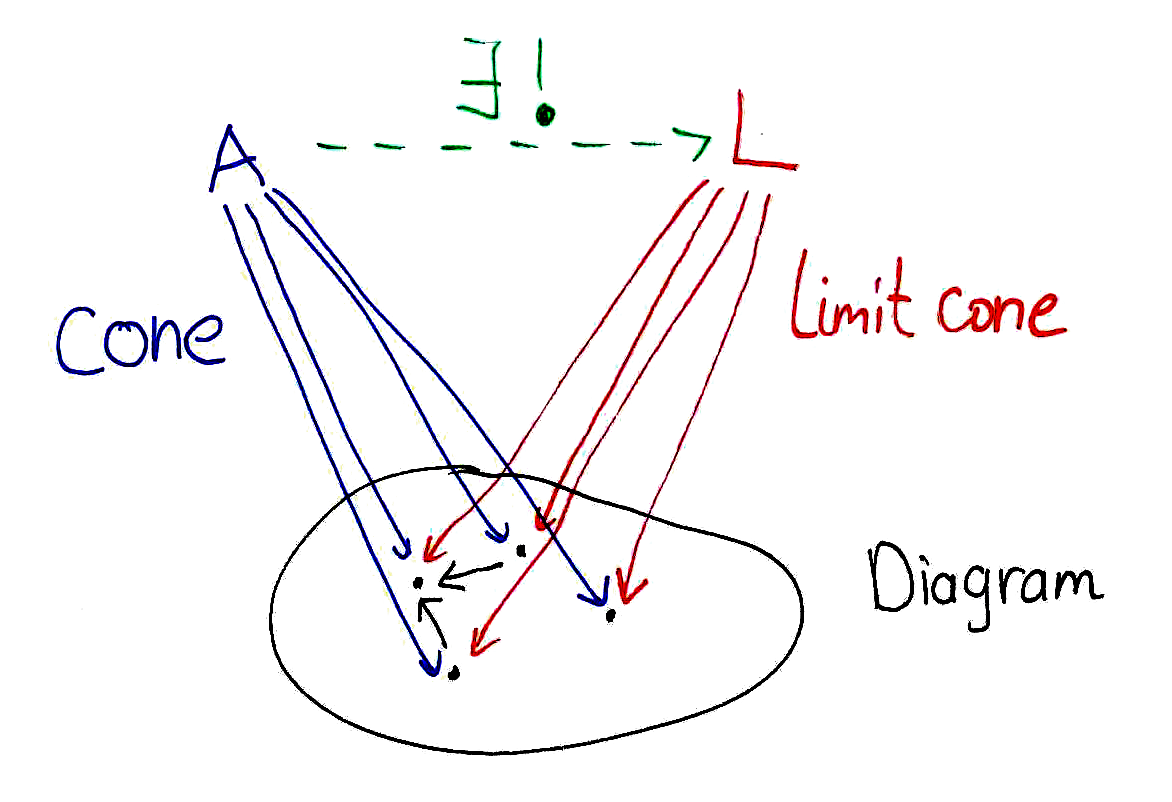
\includegraphics[scale=0.15]{Images/limits.png}
    \caption{Limit as the terminal cone over a diagram.}
    \label{fig:limits}
\end{figure}
    
\begin{example}
\begin{enumerate}
    \item $\calJ=\varnothing$ and $F$ is the empty functor into $\calC$. Then $\limit(F)$ is a terminal object in $\calC$ and $\colimit(F)$ is an initial object in $\calC$.
    \item $\calJ=(\bullet\quad\bullet)$ (discrete category with two objects). Then $\limit(F)=F(1)\times F(2)$ and $\colimit(F)=F(1)\sqcup F(2)$.
    \item $\calJ=(A\bullet\to \bullet_D\longleftarrow \bullet B$, then $\limit(F)=A\times_D B$.
    \item $F(\calJ)=(A\bullet\to \bullet B)$, then $\limit(F)=A$ and $\colimit{F}=B$.
    \item $F(\calJ)=(A\bullet\toto[\alpha]{\beta}\bullet B)$. Then $\limit(F)=\mathrm{eq}(\alpha,\beta)=\{a\mid \alpha(a)=\beta(a)\}$ is the equalizer and $\colimit(F)=\mathrm{coeq}(\alpha,\beta)=B/(\alpha(a)\sim \beta(a))$ is the coequalizer.

\end{enumerate}
\end{example} 

\begin{defn}[Preservation of limits]
    A covariant functor $G:\mathcal{C}\to\mathcal{D}$ preserves the limits of the functor $F:\mathcal{J}\to \mathcal{C}$ if $\limit(G\circ F)=G \limit(F)$. Recall that a limit consists of an object and a set of morphisms from that object that make up the limit cone, so $G$ also acts on these morphisms. Preservation of colimits is defined analogously.

    $G$ is said to preserve all $J$-shaped (co)limits if it preserves the (co)limits of all functors $F:\mathcal{J}\to \mathcal{C}$. 

    Note that for contravariant functors the analogous concepts would be functors that take limits to colimits, or colimits to limits.
\end{defn}    
\begin{defn}[Continuous functors]\index{Continuous functor}
    A functor is called (co)continuous if it preserves all \emph{small (co)limits} (that is, $J$-shaped (co)limits for all categories $J$ such that $\mathrm{Ob}(J)$ is a set and not a proper class).
\end{defn}
\begin{thm}[Continuity of hom-functors]
    Covariant hom-functors $h^A:B\mapsto \mathrm{Hom}_{\mathcal{C}}(A,B)$ preserve all limits. Similarly, contravariant hom-functors take colimits to limits.
\end{thm}
\begin{rem}
     Note that the same is not generally true for colimits -- e.g.\ $h^A(B\sqcup C)\neq h^A(B)\sqcup h^A(C)$ in $\mathsf{Set}$.
\end{rem}
\begin{cor}
    Combining the above theorem with Yoneda's Lemma \ref{Yoneda}, we conclude that all representable covariant functors preserve all limits. Similarly, representable contravariant functors map all colimits to limits.
\end{cor}
\begin{thm}\label{thm diagonal functor adjoint to limit}
    Recall that $\mathcal{C}^\mathcal{J}$ is the category of $J$-shaped diagrams in $\mathcal{C}$, i.e.\ covariant functors from $\mathcal{J}$ to $\mathcal{C}$ (see Example \ref{categories of diagrams}). Suppose that for each functor $F:\mathcal{J}\to\mathcal{C}$ the limit $\limit F$ exists in $\mathcal{C}$. Then the \emph{diagonal functor} which assigns to each object $A$ the \emph{constant diagram} $\underline A\in \mathcal{C}^\mathcal{J}$ (i.e.\ all objects of $\mathcal{J}$ are mapped to $A$ and all morphisms to $\mathrm{id}_A$),
    \[\Delta: \mathcal{C}\to \mathcal{C}^{\mathcal{J}};\; A\mapsto \underline{A},\]
    is left adjoint to the limit functor
    \[\limit: \mathcal{C}^\mathcal{J}\to \mathcal{C};\; F\mapsto \limit F\]
    (this functor forgets the morphisms associated with the limiting object).
\end{thm}
\begin{proof}
    For the bijection 
    \[
        \Hom_{\mathcal{C}^\mathcal{J}}(\underline{A},F)\cong \Hom_{\mathcal{C}}(A,\limit F),\label{limit functor bijection}
    \]
    note that a natural transformation $\tau: \underline{A}\Longrightarrow F$ (which is what morphisms in $\mathcal{C}^\mathcal{J}$ are) with component morphisms $\tau_j:A\to F(j)$ ($j$ ranges over all objects in $\mathcal{J}$) corresponds to a unique morphism $\limit \tau: A\to \limit F$ in $\mathcal{C}$. Conversely, a morphism $l:A\to \limit F$ determines a unique natural transformation $\tau:\underline{A}\Longrightarrow F$ such that $l=\limit \tau$, namely its components are $\tau_j=l\pi_j$ given the morphisms $\pi_j$ included in the definition of $\limit F$. It is easy to check that this bijection is natural in $A$.
\end{proof}
\begin{cor}\label{corollary on limits}
    The natural bijection (\ref{limit functor bijection}) (with some object $L$ from $\mathcal{C}$ instead of $\limit F$ to avoid confusion) holds for each object $A$ in $\mathcal{C}$ iff the functor $F$ has a limit.
\end{cor}
\begin{proof}
    The existence of the limit is equivalent to the existence of a unique morphism $\limit \tau: A\to L$ for each natural transformation $\tau:\underline{A}\to F$.
\end{proof}
\begin{rem}
    Since a morphism (natural transformation) $\underline{A}\Longrightarrow F$ in the category $\mathcal{C}^\mathcal{J}$ is the same as a cone from $A$ to $F$, the limit $\limit F$ can be defined as the universal natural transformation $\Delta \Longrightarrow F$. Similarly, colimits are the universal natural transformations $F\Longrightarrow \Delta$.
\end{rem}
\begin{thm}[Continuity of adjoint functors]\label{continuity of adjoints thm}
    Every functor that has a left adjoint (and therefore is a right adjoint) is continuous. The dual statement is that every functor that has a right adjoint (and therefore is a left adjoint) is cocontinuous.
\end{thm}
\begin{proof}
    Let $R:\mathcal{C}\to \mathcal{D}$ be the right adjoint to $L:\mathcal{D}\to\mathcal{C}$. Suppose that $\limit F$ exists in $\mathcal{C}$. For each object $A$ in $\mathcal{C}$, a natural bijection
    \[\Hom_{\mathcal{C}^\mathcal{J}}(\underline{L(A)},F)\cong \Hom_{\mathcal{D}^\mathcal{J}}(\underline{A},R\circ F) \label{adjunction bijeciton}\]
    is provided by the natural adjunction bijection
    \[\Hom_{\mathcal{C}}(L(A),F(j))\cong \Hom_{\mathcal{D}}(A,R(F(j))\]
    for each object $j$ in $\mathcal{J}$, sending the component $h_j$ of an element of the l.h.s.~of (\ref{adjunction bijeciton}) to the corresponding component of the natural transformation on the right. Now consider the string of natural bijections
    \begin{multline}
        \Hom_{\mathcal{D}^\mathcal{J}}(\underline{A},R\circ F)\cong \Hom_{\mathcal{C}^\mathcal{J}}(\underline{L(A)},F)\cong \\ 
        \cong \Hom_{\mathcal{C}}(L(A),\limit F)\cong \Hom_{\mathcal{D}}(A,R(\limit F))
    \end{multline}
    coming respectively from (\ref{adjunction bijeciton}), (\ref{limit functor bijection}), and the adjunction. By Corollary~\ref{corollary on limits} combined with the uniqueness of adjoints (Proposition~\ref{uniqueness of adjoints prop}), we have $\limit(R\circ F)= R(\limit F)$ as required.
    % Let $G:\mathcal{D}\to\mathcal{C}$ be a left adjoint, i.e.\ $G^\ast$ exists. Then for a colimit $\colimit(F)$ of $F:\mathcal{J}\to \mathcal{D}$, by continuity of hom-functors, we have
    % \begin{multline}
    %     \Hom_{\mathcal{C}}(G\colimit F,B)\cong \Hom_{\mathcal{D}}(\colimit F,G^\ast(B))\cong \limit \Hom_{\mathcal{D}}(F,G^\ast(B)) \cong \\\cong \limit \Hom_{\mathcal{C}}(G\circ F,B)\cong \mathrm{Cocones}(G\circ F,B),
    % \end{multline}
    % and these bijections are natural in $B$. However, the existence of a natural bijection with the set of cones from $G\circ F$ is exactly the characteristic property of a colimit (see definition).
\end{proof}
\begin{cor}
    Limits commute with limits (assuming all limits of the necessary shapes exist). Colimits commute with colimits.
\end{cor}
\begin{proof}
    Viewing the limit is a functor  $\limit:\calC^J\to \calC$, we have just shown that it is right adjoint to the diagonal functor (a.k.a.~the constant diagram functor). Therefore it is continuous, i.e.~commutes with limits. 
\end{proof}

Note that limits and colimits typically do not commute.

\begin{example}[Siefert-van Kampen theorem redux]\index{Theorem!Siefert-van~Kampen}
    We've learned by now that contravariant representable (or hom-) functors map colimits to limits, so they're not the functors that preserve colimits. It is the left adjoints that do. Siefert-van~Kampen theorem essentially states that the fundamental functors $\pi_1$ or $\Pi$ preserve \emph{some} colimits (namely pushouts). 
    
    While not a proof, one categorical source of intuition for this is that both of these functors are left adjoints. The reason $\pi_1$ preserves only pushouts, and not all colimits, is that the functor that maps the category $\mathsf{Top}$ into the homotopy category $\mathsf{hTop}$ doesn't preserve colimits, so $\pi_1$ doesn't either. However, the descended version of this functor, $\pi_1:\mathsf{hTop}\to \mathsf{Gr}$ happens to be the left adjoint of a certain functor that constructs a topological space given a group. Looking far ahead, this is the functor $B:G\mapsto BG$ that constructs the classifying space of $G$. It is so called because $BG$ is the base space of a universal principal $G$-bundle such that any other $G$-bundle is a pullback along some continuous map into $BG$. For example, universal covering spaces are exactly the classifying spaces for the fundamental groups of their base -- e.g.\ $B\bbZ=\bbS^1$ and $B(\bbZ\ast \bbZ)=\bbS^1\vee \bbS^1$ etc. $BG$ is in fact the unique (up to ``weak'' homotopy equivalence) space whose fundamental group is $G$ and all other homotopy groups are trivial (which also identifies it with the first  Eilenberg-MacLane space $K(G,1)$).

    So, by a happy coincidence, pushouts in the homotopy category lined up with pushouts in the original topological category.
\end{example}

The most common examples of infinite limits and colimits are ones where $\mathcal{J}$ can be indexed by integers.

\begin{defn}[Direct and inverse limits]\index{Limit!direct}\index{Limit!inverse}
    If $\calJ$ is a directed system and $F:\calJ\to \calC$ a functor, then $\colimit(F)$ is called a direct, or an inductive, limit. It is also often written as $\colimit A_j$, where $A_j=F(j)$.
    
    If $\calJ$ is an inverse system (i.e.~$\calJ^{\mathrm{op}}$ is a directed system), then $\limit(F)$ is called an inverse, or a projective, limit.
    
    More generally, if $\calJ$ is a poset category (see Example \ref{poset example}), then it is said to be directed to the right (left) if $\forall i,j\in \ob(\calJ)$ $\exists k\in \ob(\calJ)$ such that $i,j\leq k$ (respectively, $k\leq i,j$). Then one can define direct limits of diagrams directed to the right and inverse limits of diagrams directed to the left.
\end{defn}


\begin{example}
\begin{enumerate}
    \item In $\colimit$, most commonly all arrows are monomorphisms. For example, consider the category $\mathsf{Gr}$ of groups and the sequence $S_n$ of symmetric groups with the embeddings $S_n\hookrightarrow S_m$ for every $n<m$ defined as permutations of the first $n$ symbols. Then $\colimit(S_n)=S_\infty$, which is the group of all permutations of $\mathbb{N}$ of finite support.
    
    Alternatively, we can define another partial order on the set of symmetric groups $S_n$. Namely, define $n\preccurlyeq m\Leftrightarrow n\mid m$ and the inclusion $S_n\hookrightarrow S_m$ by $m/n$ copies of the permutation. Then $\colimit (S_n)$ is a different group.
    \item For any unital ring $R$, the direct limit of the general linear matrix groups over $R$ (where matrices of size $n$ are embedded into groups of larger matrices by filling in the diagonal with ones) is $\colimit(\GL(n,R))=\GL(R)$, the \emph{quite general linear group} of $R$.
    \item In $\mathsf{Set}$, direct limits are simply infinite unions factored by identifying elements with coincident ``descendants'', i.e. $\colimit A_i=\bigsqcup_i A_i/\sim$, where $x\in A_i$ is equivalent to $y\in A_j$ iff $\exists f_{jk},f_{jk}$ such that $f_{ik}(x)=f_{jk}(y)$. The inverse limit is the set of infinite sequences of descendants $\limit (A_i)=\{(a_i)\mid a_i\in A_i,\forall i\leq j, f_{ij}(a_i)=a_j\}$.
    \item Consider the polynomial ring $K[t]$ over a field $K$ and its factor rings $K[t]/t^n$ of truncated polynomials. Then we have the sequence of epimorphisms 
    \[\cdots \to K[t]/t^3\to K[t]/t^2\to K,\]
    and the inverse limit is $\limit(K[t]/t^n)=K[[t]]$, which is the ring of \emph{all} formal power series $\sum_{i\geq 0}a_i t^i$. This illustrates the more general fact that projective limits are generally enormous, so much so that the cardinality of the limit is often higher than of any object in the sequence.
    \item Let $p$ be a prime integer and consider the sequence of groups
    \[\cdots\to \bbZ/p^3 \bbZ\overset{\mod p^2}\to \bbZ/p^2\bbZ\overset{\mod p}\to \bbZ/p\bbZ.\]
    Then $\limit(\bbZ/p^n\bbZ)=\bbZ_p$ is the group of $p$-adic integers (it has the cardinality of continuum!).
    \item Consider the poset diagram directed to the left consisting of group epimorphisms $\bbZ/m\bbZ\overset{\mod n}\to \bbZ/n\bbZ$ for $n\mid m$. Then 
    $\limit (\bbZ/n\bbZ)=\hat{\bbZ}$ is the \emph{profinite completion of $\bbZ$}.
    \item The monomorphism sequence $\bbZ/p^n\bbZ\overset{\cdot p}\to \bbZ/p^{n+1}\bbZ$ gives the direct limit $\colimit(\mathbb{Z
    }/p^n\bbZ)=\bbZ(p^\infty)$, which is called a Pr\"ufer group (it can be realized as the group of all roots of unity of the form $\exp(2\pi\rmi \cdot m/p^n)$).
    \item In topological and geometric categories, direct limits are similar to unions (when they exist). For instance, the $n$-sphere can be embedded $\bbS^n\hookrightarrow \bbS^{n+1}$ as the equator, and the direct limit gives $\bbS^\infty=\colimit \bbS^n$.
\end{enumerate}
\end{example}





\subsection{Sub-objects and quotient objects}

\begin{defn}
    Let $X,U,V\in\ob(\calC)$ and consider a diagram
    \[\begin{tikzcd}[every matrix/.append style={name=m},   
        execute at end picture={\draw [<-] ([xshift=-2mm,yshift=-12mm]m-1-2.north) arc[start angle=-90,delta angle=-270,radius=0.25cm];}]
        U \arrow[dr,tail,"u\text{, mono}"]& \\
        & X\\
        V\arrow[uu,tail,dashed,"\exists h"]\arrow[ur,tail,swap,"v\text{, mono}"]& 
\end{tikzcd}\]
    We say that $v\leq u$ if there exists a morphism $h$ such that $v=u\circ h$ ($h$ has to be a monomorphism for this to hold).
\end{defn}

Here are the properties of this relation:
\begin{enumerate}
    \item $u\leq u$;
    \item $u\leq v,v\leq w\Rightarrow u\leq w$;
    \item $u\leq v,v\leq u\Rightarrow U\overset{f}{\cong} V$, where $u=v\circ f$ and $v=u\circ f^{-1}$.
    \begin{proof}
        We have $V\overset{h}{\to}U$ and $U\overset{g}{\to}V$.
        
        On the one hand, $v=u\circ h=v\circ g\circ h\Rightarrow g\circ h=1_V$ since $v$ is mono.
        
        On the other hand, $u=u\circ(h\circ g)\Rightarrow h\circ g=1_U$ since $u$ is mono.
    \end{proof}
\end{enumerate}

\begin{defn}[Sub-objects]\index{Sub-object}
    Introduce an equivalence relation on monomorphisms: $u\sim v$ iff $u\leq v$ and $v\leq u$. Then a sub-object of $X$ is an equivalence class of pairs $(U,u)$, where $u:U\to X$ is a mono.
\end{defn}

\begin{example}
    $\bbZ\overset{\cdot n}\to \bbZ$ is mono and defines the group $n\bbZ$ as a sub-object of $\bbZ$.
\end{example}

\begin{defn}[Quotient objects]\index{Quotient object}
    For epimorphisms, we define the relation $y\geq z$ if in the diagram 
    \[\begin{tikzcd}[every matrix/.append style={name=m},   
        execute at end picture={\draw [<-] ([xshift=-6mm,yshift=-5mm]m-2-2.north) arc[start angle=-90,delta angle=-270,radius=0.25cm];}]
        & Y \arrow[dd,two heads,dashed,"\exists h"] \\
        X\arrow[dr,two heads,swap,"z\text{, epi}"]\arrow[ur,two heads,"y\text{, epi}"] &\\
        & Z 
    \end{tikzcd}\]
    there exists such a morphism $h$ that $z=h\circ y$ (it has to be epi).
    Then a quotient object of $X$ is an equivalence class of pairs $(Y,y)$, where $y:X\to Y$ is epi.
\end{defn}

\begin{example}
    There are many different epimorphisms $\bbZ^2\to\bbZ$. They define many non-equivalent quotient objects of $\bbZ^2$, each isomorphic to $\bbZ$.
\end{example}



\subsection{Abelian categories}

Abelian categories are, roughly speaking, categories where objects and morphisms form abelian groups themselves, and where the First Isomorphism theorem holds. Examples include $\mathsf{Ab}$, $\mathsf{Vect}_K$, $R-\mathsf{Mod}$ or $\mathsf{Mod}-R$, $\mathsf{SheafAb}$. Notably, $\mathsf{TopAb}$ is not abelian because the First Isomorphism theorem generally doesn't hold for topological groups (we call such a category pre-abelian).

\begin{defn}[Abelian categories]\index{Abelian category}
    A category $\calC$ is called abelian if:
    \begin{enumerate}
        \item Every morphism set $\mor(A,B)$ has the structure of an abelian group, i.e. morphisms can be added and subtracted.
        \item There exists a zero object $0\in\ob(\calC)$.
        \item The product and coproduct of any two objects exist and are isomorphic. The result is denoted by the direct sum: $A\times B\cong A\sqcup B \equiv A\oplus B$.
        \item All equalizers and coequalizers exist. In particular, using the abelian property, we define
        \[\ker (\varphi)\coloneqq\mathrm{eq}(\varphi,0),\quad \coker(\varphi)\coloneqq\mathrm{coeq}(\varphi,0).\]
        \item The image and coimage of any morphism coincide, $\im (\varphi)=\coim(\varphi)$. These will be defined below.
    \end{enumerate}
\end{defn}

We can give alternative definition of kernels and cokernels.
\begin{defn}[Kernel]\index{Kernel}
    Let $X\overset\varphi\to Y$ be a morphism in an abelian category. Then $\ker\varphi$ is the sub-object $(K,k)$ of $X$ such that $\varphi\circ k=0$ and it is universal with this property:
    \[\begin{tikzcd}[every matrix/.append style={name=m},   
        execute at end picture={\draw [<-] ([xshift=-10mm,yshift=-8mm]m-1-2.north) arc[start angle=-90,delta angle=-270,radius=0.15cm];}]
        K \arrow[r,tail,"k"]& X\arrow[r,"\varphi"] & Y\\
        Z\arrow[u,dashed,"\exists! h"]\arrow[ur,swap,"\forall\psi:\,\varphi\circ\psi=0"]& & 
    \end{tikzcd}\]
    (such a $h$ is automatically unique for every $\psi$ because $k$ is mono).
\end{defn}

\begin{defn}[Cokernel]\index{Cokernel}
    Let $X\overset\varphi\to Y$ be a morphism in an abelian category. Then $\coker\varphi$ is the quotient object $(C,c)$ of $Y$ such that $c\circ\varphi=0$ and it is universal with this property:
    \[\begin{tikzcd}[every matrix/.append style={name=m},   
        execute at end picture={\draw [<-] ([xshift=-4mm,yshift=-8mm]m-1-3.north) arc[start angle=-90,delta angle=-270,radius=0.15cm];}]
        X\arrow[r,"\varphi"] & Y \arrow[r,two heads,"c"]\arrow[dr,swap,"\forall\psi:\,\psi\circ\varphi=0"]  & C\arrow[d,dashed,"\exists! h"] \\
        & & Z
    \end{tikzcd}\]
    (such a $h$ is automatically unique for every $\psi$ because $c$ is epi).
\end{defn}

\begin{example}
    It is easy to check that in the category $\mathsf{Ab}$ of abelian groups, $\coker\varphi=H/\varphi(G)$ for $\varphi:G\to H$. Thus the last axiom of abelian categories is equivalent to the First Isomorphism theorem in this case. Note that this factor doesn't exist neither in $\mathsf{Gr}$ nor in $\mathsf{TopAb}$.
    
    The same formula holds for all ring modules. In $\mathsf{Gr}$ (which is not an abelian category, but in which kernels and cokernels can be similarly defined), the cokernel is the quotient by the normal closure of the image.
\end{example}

This allows us to define images and coimages.

\begin{defn}[Image, coimage]\index{Image of a morphism}\index{Coimage of a morphism}
    In abelian categories, $\im\varphi$ for a morphism $\varphi:X\to Y$ is the sub-object of $Y$ defined as
    \[\im(\varphi)=\ker(\coker\varphi),\quad\quad K\overset k \rightarrowtail X\overset\varphi\to Y\overset c\twoheadrightarrow C.\]
    Similarly, $\coim\varphi$ is the quotient object of $X$ defined as 
    \[\coim(\varphi)=\coker(\ker\varphi).\]
\end{defn}

Note that
\[\ker(\coim\varphi)=\ker(\coker(\ker\varphi)))=\im(\ker\varphi).\]
Thus in general pre-abelian categories (i.e.\ without the last axiom) by the universal properties of images and coimages we have a factorization of any morphism $\varphi:X\to Y$ into the sequence
\[\ker\varphi\rightarrowtail X\underbrace{\overset{\text{epi}}\twoheadrightarrow\coim\varphi\overset{\text{bi}}\to\im\varphi\overset{\text{mono}}\rightarrowtail}_\varphi Y\twoheadrightarrow\coker\varphi \]
The last axiom of abelian categories states that $\coim\varphi = \im\varphi$, which is equivalent to the statement:
\[\boxed{\text{5. All bimorphisms are isomorphisms.}}\]
\begin{xca}
    Prove that the last axiom of abelian categories is indeed equivalent to the boxed statement.
\end{xca}
Therefore only in abelian categories we have the decomposition
\[\ker\varphi\to X \overset{j\text{, epi}}\longrightarrow\im\varphi\overset{i\text{, mono}}\longrightarrow Y\to \coker\varphi,\]
where
\[\text{factorization property}:\quad \varphi=i\circ j,\quad i\text{ -- mono}, j\text{ -- epi}.\]

\begin{defn}[Additive functor]
    A functor $F:\calC\to\calD$ between two abelian categories is called additive if for any $A,B\in\ob(\calC)$, the map $F_{A,B}:\Hom_\calC(A,B)\to \Hom_\calD(F(A),F(B))$ defined by $\varphi\mapsto F_{A,B}(\varphi)=F(\varphi)$ is a homomorphism of abelian groups.
\end{defn}

The following theorem is the main general result about abelian categories and effectively states that all abelian categories can be realized as (almost arbitrarily nice) full subcategories of categories of ring modules. It is essentially a much stronger version of the Yoneda Lemma~\ref{Yoneda} for abelian categories.

\begin{thm}[Freyd-Mitchell]
    For any abelian category $\calC$ there exists a ring $R$ and a functor $F:\calC\to R\text{-}\mathsf{Mod}$ that is: additive, full and faithful (surjective and injective on sets of morphisms for each pair of objects), preserves kernels, cokernels, products and coproducts, is exact (preserves exact sequences, see below)...
\end{thm}
This theorem justifies all diagrammatic methods that we will develop in the next two sections: since $R\text{-}\mathsf{Mod}$ is a concrete category, its objects are sets. Therefore by the Freyd-Mitchell theorem, it suffices to prove any general statement about abelian categories only for categories of ring modules, which allows us to refer to elements of objects as sets, and apply morphisms as functions to those elements! It is a way to completely side-step so called ``abstract nonsense'' proofs that deliberately avoid talking about elements of objects as if they are sets.






\newpage
\section{Homological Algebra I: Exactness}

\subsection{Exact sequences and functors}

From now on in this Part we work only with abelian categories. In fact, homological algebra can be viewed as the extension of linear algebra to all abelian categories.

\begin{defn}[Exact sequences]\index{Exact sequence}
    A sequence of morphisms in an abelian category 
    \[\cdots \to A_{i-1}\overset{\alpha}\to A_i\overset{\beta}\to A_{i+1}\to \cdots\]
    is called exact in $A_i$ if 
    \[\im\alpha=\ker\beta.\]
    A sequence is just called exact if it is exact in every object in it.
\end{defn}

\begin{prop}
    \begin{enumerate}
        \item A sequence $0\to A\overset f\to B$ is exact iff $f$ is mono;
        \item A sequence $A\overset f\to B\to 0$ is exact iff $f$ is epi;
        \item A sequence $0\to A\overset f\to B\to 0$ is exact iff $f$ is an isomorphism;
        \item A sequence $0\to A\to B\overset f\to C\to D\to 0$ is exact iff $A=\ker f$ and $D=\coker f$.
    \end{enumerate}
\end{prop}
\begin{proof}
    Exercise.
\end{proof}

\begin{defn}[Short exact sequences]\index{Exact sequence!short}
 A short exact sequence is an exact sequence of the form
 \[0\to A\overset f\rightarrowtail B\overset g \twoheadrightarrow C\to 0.\]
 Such a sequence (and the object $B$ in particular) is also called an \emph{extension} of $A$ by $C$. The exactness of this sequence is equivalent to $f$ being mono, $g$ being epi, and $\im f=\ker g$.
\end{defn}

\begin{prop}[First isomorphism theorem]
    If $0\to A\overset f\to B\overset g \to C\to 0$ is a short exact sequence, then 
    \[A\cong \im f,\quad C\cong B/\im f.\]
\end{prop}
\begin{proof}
    The first isomorphism is known in concrete categories, which is sufficient. It states that $B/\ker g\cong \im g$, and by exactness $\ker g=\im f$ and $\im g=C$, thus $B/\im f\cong C$.
\end{proof}

\begin{defn}[Split sequence]\index{Split sequence}
 A short exact sequence $0\to A\overset i\to B\overset p \to C\to 0$ is called split if there exists a morphism $j:C\to B$ with $p\circ j=1_C$, i.e. if $p$ is a split epi.
\end{defn}

\begin{prop}[Rank-nullity theorem]\index{Theorem!Rank-nullity}
    If a short exact sequence $0\to A\overset i\to B\overset p \to C\to 0$ is split, then $B\cong A\oplus C$.
\end{prop}
\begin{proof}
    We show that $B\cong \im i\oplus \im j$, where $j$ is a section for $p$. We perform a simple \emph{diagram chasing} by considering an element $b\in B$:
    \begin{multline}
        b\in B\implies p(b-j\circ p(b))=p(b)-\underbrace{p\circ j}_{1_C}(p(b))=\\=0\implies b-j\circ p(b)\in\ker p\overset{\text{exact}}{\implies}\exists a\in A: i(a)=b-j\circ p(b).
    \end{multline}
    This proves that $B=\im i+\im j$. To prove that $\im i\cap \im j=\{0\}$, suppose $x=i(a)=j(c)$. Then $p(x)=p(i(a))=0$ since $p\circ i=0$, and at the same time $p(x)=p(j(c))=c$ since $p\circ j=1_C$. Thus $c=0$, $x=j(c)=0$, and $B\cong A\oplus C$.
\end{proof}

\begin{prop}[Rank-nullity for vector spaces]\label{gen rank-nullity}
    If $0\to A_1\overset{f_1}\to A_2 \overset{f_2}\to\cdots A_n\to 0$ is an exact sequence of finite dimensional vector spaces, then
    \[\sum_{i=1}^n(-1)^i \dim A_i=0.\]
\end{prop}
\begin{proof}
    By the standard rank-nullity theorem, the l.h.s.\ equals \[\sum_{i=1}^{n-1}(-1)^i\dim \ker f_i+\sum_{i=1}^{n-1}(-1)^i\dim \im f_i.\] By exactness, this sum vanishes.
\end{proof}


\begin{comment}
    \begin{samepage}
        \PRLsep
        \begin{center}
            {\red Lecture 19 on 26 Apr 2019 ended here}
        \end{center}
    \end{samepage}
\end{comment}



\begin{defn}[Exact functors]\index{Exact functor}
 A functor $F:\calC\to\calD$ is called exact if it maps every exact sequence into an exact sequence.
\end{defn}

\begin{prop}
    For an additive functor $F$ to be exact it suffices to be exact on short sequences.
\end{prop}
\begin{proof}
    The idea of the proof is to expand any segment of an exact sequence $A\to B\to C$ into a combination of short exact sequences (this method is generally called ``splicing'' of short sequences).
    
    Namely, we have the following \emph{commutative} diagram with exact diagonals:
    \[\adjustbox{scale=0.8,center}{\begin{tikzcd}
        0 \arrow[dr]& & & & 0 \arrow[dr]& & 0 & & \\ 
        & \ker f \arrow[dr]&&&& \im g \arrow[dr]\arrow[ur]&&&\\
        && A \arrow[rr,"f"]\arrow[dr]&& B \arrow[rr,"g"]\arrow[ur] && C \arrow[dr] &&\\
        &&& \im f\arrow[dr]\arrow[ur] &&&& \coker g\arrow[dr]&\\
        && 0 \arrow[ur] && 0 &&&& 0
    \end{tikzcd}}\]
    Applying $F$, we get the \emph{commutative} diagram
    \[\adjustbox{scale=0.8,center}{\begin{tikzcd}[row sep=normal, column sep = small]
        0 \arrow[dr]& & & & 0 \arrow[dr]& & 0 & & \\ 
        & F(\ker f) \arrow[dr]&&&& F(\im g) \arrow[dr]\arrow[ur]&&&\\
        && F(A) \arrow[rr,"F(f)"]\arrow[dr]&& F(B) \arrow[rr,"F(g)"]\arrow[ur] && F(C) \arrow[dr] &&\\
        &&& F(\im f)\arrow[dr]\arrow[ur] &&&& F(\coker g)\arrow[dr]&\\
        && 0 \arrow[ur] && 0 &&&& 0
    \end{tikzcd}}\]
    with exact diagonals. Now we notice
    \begin{multline}
        \im F(f)=\im\left(F(A)\to F(\im f)\to F(B)\right)=\im(F(\im f)\to F(B))=\\
        =\ker (F(B)\to F(\im g))=\ker (F(B)\to F(\im g)\to F(C))=\ker F(g),
    \end{multline}
    where the second equality follows from $F(A)\to F(\im f)$ being epi and the next to last equality holds since $F(\im g)\to F(C)$ is mono. Therefore $F(A)\to F(B)\to F(C)$ is exact.
\end{proof}

There are in fact very few exact functors. Here are a few relevant examples.

\begin{example}
    \begin{enumerate}
        \item Let $G\text{-}\mathsf{Ab}$ be the category of abelian groups with a $G$-action (morphisms in it are equivariant homomorphisms $f(g\cdot a)=g\cdot f(a)$). Then we can define the functor that for every group $A$ with a $G$-action produces its subgroup of invariants $A^G$:
        \[A^G=\{a\in A\mid \forall g\in G,\; g\cdot a=a\}.\]
        (The action on morphisms is trivial.) This is a functor $G\text{-}\mathsf{Ab}\to\mathsf{Ab}$. Now let us consider a short exact sequence
        \[0\to A\to B\to B/A\to 0.\]
        Its image is clearly not exact on the right:
        \[0\to A^G\to B^G\to (B/A)^G \cancel{\to} 0.\]
        Indeed, $(B/A)^G$ are $G$-invariant only up to addition of elements of $A$, whereas $B^G/A^G$ (which is what we would have in a short exact sequence) is a totally different group consisting of classes of truly $G$-invariant elements. We say that this functor is only \emph{left exact}.
        \item The representable (hom-)functors $\Hom_{R\text{-}\mathsf{Mod}}(\_,\_)$ acting $R\text{-}\mathsf{Mod}\times R\text{-}\mathsf{Mod}\to \mathsf{Ab}$ with either argument fixed can act on a short exact sequence 
        \[0\to A\to B\to C\to 0\]
        to give two exact sequences
        \begin{eqnarray}
            0\to \Hom(X,A)\to \Hom(X,B)\to \Hom(X,C),\\
            0\to \Hom(C,Y)\to \Hom(B,Y)\to \Hom(A,Y).
        \end{eqnarray}
        Therefore Hom-functors are also only left exact. Indeed, right exactness for them would mean that every morphism $X\to C$ or $A\to Y$ can be factored through $B$, which we know to be false. For example, consider
        \[\begin{tikzcd}
        0\arrow[r]& A=\bbZ\arrow[r,"\text{incl.}"]\arrow[d,
        "\id"]& B=\frac{1}{n}\bbZ\arrow[dl,dashed,"?"] \\
         &Y=\bbZ &
        \end{tikzcd}\]
        For right exactness, $\id:A\to Y$ would need to factor through $B$, which is clearly impossible here.
        
        An analogous example for the first line is
        \[\begin{tikzcd}
        B=\bbZ\arrow[r,"\mod n"] & C=\bbZ/n\bbZ\arrow[r] & 0 \\
         &X=\bbZ/n\bbZ\arrow[ul,dashed,"?"]\arrow[u,
        "\id"] &
        \end{tikzcd}\]
        If this functor were to be surjective on Hom-sets, every map $X\to C$ would have to come from a map $X\to B$, which is clearly false in this case.
        \item The tensor product functor $\_\otimes\_:\mathsf{Mod}\text{-}R\times R\text{-}\mathsf{Mod}\to \mathsf{Ab}$ is also not exact. In fact it is only \emph{right exact}: for every short exact sequence
        \[0\to A\to B\to C\to 0\]
        it gives two exact sequences (in fact they are the same because $X\otimes Y$ is naturally isomorphic to $Y\otimes X$)
        \begin{eqnarray} 
        X\otimes A\to X\otimes B\to X\otimes C\to 0,\\
        A\otimes Y\to B\otimes Y\to C\otimes Y\to 0.
        \end{eqnarray}
        We will give an example that shows that this functor is not left exact in Example \ref{non-flat module example}.
    \end{enumerate}
\end{example}


\begin{defn}[Projective and injective objects]\index{Projective object}\index{Injective object}
    If the functor $\Hom(X,\_)$ is exact, $X$ is called a projective object (i.e.\ all morphisms $X\to C$ factor through $B$ in any exact sequence $B\to C\to 0$). If $\Hom(\_,Y)$ is exact, $Y$ is called an injective object (all morphisms $A\to Y$ factor through $B$ in any exact sequence $0\to A\to B$).
\end{defn}

\begin{defn}[Flat module]\index{Flat module}
    An object $X$ is called \emph{flat} if the functor $X\otimes\_$ (or equivalently $\_\otimes X$) is left exact.
\end{defn}

\begin{example}\label{non-flat module example}
    Consider in the category of $\bbZ$-modules the sequence on the left and its image under a tensor product with $\bbZ/n\bbZ$
    \[0\to \bbZ\overset{\cdot n}\to \bbZ \quad \overset{\otimes\bbZ/n\bbZ}\rightsquigarrow \quad \bbZ\otimes \bbZ/n\bbZ\overset{\cdot n}\to\bbZ\otimes \bbZ/n\bbZ.\]
    The arrow on the right is obviously not mono (it is the zero morphism), therefore $\bbZ/n\bbZ$ is not a flat $\bbZ$-module.
\end{example}

The moral of these examples is that whereas in categories of vector spaces $\mathsf{Vect}_K$ everything would be exact, exactness is generically broken as soon as we pass to structures over rings. The study of ring modules is a natural extension of linear (matrix) algebra over fields, and largely reduces to homological algebra.
\[
\boxed{\begin{array}{c}
\text{The goal of homological algebra is:}\\
\text{to characterize the obstructions to the exactness of certain additive functors}\\ \text{(these obstructions are called derived functors).}
\end{array}}
\]
Given a non-exact functor, the values of its derived functors need to be added into the image of a short exact sequence to produce a fully exact (albeit potentially infinitely long) sequence. For example, in the case of the invariants functor, every short exact sequence $0\to A\to B\to B/A\to 0$ becomes a \emph{long exact sequence of group cohomology}
\[
\scriptstyle
0\to A^G\to B^G\to (B/A)^G\to H^1(G,A)\to H^1(G,B)\to H^1(G,B/A)\to H^2(G,A)\to\cdots
\]
For the Hom functor, the obstruction to right exactness is evaluated by the Ext-functors (the name comes from ``extension''):
\begin{gather}
    \scriptstyle
    0\to \Hom(X,A)\to \Hom(X,B)\to\Hom(X,C)\to \Ext^1(X,A)\to \Ext^1(X,B)\to\Ext^1(X,C)\to\cdots,\\
    \scriptstyle
    0\to \Hom(C,Y)\to \Hom(B,Y)\to\Hom(A,Y)\to \Ext^1(C,Y)\to \Ext^1(B,Y)\to\Ext^1(A,Y)\to\cdots
\end{gather}
Finally, for the tensor functor, the obstruction to left exactness is evaluated by the Tor-functors (``torsion''):
\[
\scriptstyle
\cdots\to \Tor_2(C,X)\to \Tor_1(A,X)\to \Tor_1(B,X)\to\Tor_1(C,X)\to A\otimes X\to B\otimes X\to C\otimes X\to 0.
\]
All of them are examples of (co)homology theories. We will return to a proper discussion of these objects later. The takeaway so far should be: since on manifolds we are studying spaces of sections of vector bundles, which are really $C^\infty(M)$-modules, we need homological algebra to deal with the linear algebra over the ring of functions, and the (co)homology groups will measure the non-exactness of certain constructions.






\subsection{Direct limits and exactness}

\begin{defn}
    A category $\calC$ is called complete if all limits in $\calC$ with a small index category (i.e.~$\ob(\calJ)$ is a proper set and not a class) exist. $\calC$ is called cocomplete if all small colimits in $\calC$ exist.
\end{defn}

\begin{prop}[{{\cite[Prop.~5.23]{Rotman}}}]\label{prop abelian complete and cocomplete}
    Abelian categories are complete and cocomplete.
\end{prop}
\begin{proof}
    By the Freyd-Mitchell Theorem, it suffices to consider the categories of $R$-modules. 
    
    Given a $J$-shaped diagram $\{F(i)=A_i,f_{ji}=F(i\to j)\}$ of modules, let $\lambda_i$ be the natural inclusion of $A_i$ into $\bigoplus_i A_i$. 
    
    First we construct the colimit module. Define
    \[D=\left(\bigoplus_i A_i\right)\slash S,\]
    where $S$ is the submodule generated by all elements $\lambda_j\circ f_{ji}(a_i)-\lambda_i(a_i)$ with $a_i\in A_i$ and $i\to j$ an arrow in $\calJ$. The maps $\lambda_i$ induce inclusions $\alpha_i: A_i\to D$ by $a_i\mapsto \lambda_a(a_i)+S$. It is an exercise to check that $D$ satisfies the universal property, so that $D\cong \colimit F$.

    Similarly, the limit module can be constructed as the submodule of $\bigoplus_i A_i$ consisting of tuples $\{a_i\}_{i}$ such that if $i\to j$ is an arrow in $\calJ$ then $a_j=f_{ji}(a_i)$. It is easy to check that this module satisfies the universal property for $\limit F$.
\end{proof}
\begin{rem}
    More generally, a category is complete iff all products of any number of objects exist and all equalizers exist, and cocomplete iff all coproducts and all coequalizers exist. In abelian categories both products and coproducts are direct sums and obviously exist, whereas equalizers are $\ker(f-g)$ and coequalizers are $\coker(f-g)$.
\end{rem}

In abelian categories, kernels are limits (namely equalizers), and cokernels are colimits. Therefore exactness can be rephrased in terms of preservation of kernels and cokernels. The following Proposition is obvious.

\begin{prop}[{{\cite[Prop.~5.25]{Rotman}}}]
    Let be a covariant functor between abelian categories. Then $F$ preserves kernels iff it is left exact, and it preserves cokernels iff it is right exact.
\end{prop}

\begin{prop}
    In an abelian category $\calC$, the colimit functor $\colimit$ is right exact. That is, if $J$ is small ($\ob(\calJ)$ is a proper set) and $F,G,H:\calJ\to \calC$ are functors with natural transformations $F\overset{\alpha}{\Longrightarrow}G\overset{\beta}{\Longrightarrow}H$ such that the sequence 
    \[0\to F(i)\overset{\alpha_i}{\to} G(i)\overset{\beta_i}{\to} H(i)\to 0\] is exact for all $i\in\ob(\calJ)$, then the sequence
    \[\colimit F\overset{\colimit \alpha_i}\colimit G\overset{\colimit \beta_i}\colimit H\to 0\]
    is exact. Similarly, the limit functor $\limit$ is left exact.
\end{prop}
\begin{proof}
    We make use of the fact that $\colimit F$ can be constructed concretely as the quotient of $\bigoplus_i F_i$ by all $a_i-F(i\to j)(a_i)$ where $i\to j$ is any arrow coming out of $i$ in $\calJ$, $a_i\in F_i$, and $F(i\to j)(a_i)\in F_j$ are identified with their images in $\bigoplus F_i$.

    With this description, clearly the map $\colimit G(i)\to \colimit H(i)$ is surjective. Also, composing $\colimit F(i)\to \colimit G(i)\to\colimit H(i)$ is the zero map thus $\im(\colimit \alpha_i)\subset \ker(\colimit \beta_i)$.

    Conversely, let $x\in \bigoplus_i G(i)$ represent an element of $\ker(\colimit \beta)$. Let us define the maps $A=\bigoplus_i \alpha_i$ and $B=\bigoplus_i \beta_i$. Thus $B(x)\in \bigoplus H(i)$ is a finite sum of elements of the form $p_i-G(i\to j)(p_i)$. Since $\beta_i$ is surjective, we can write such a term as 
    \[\beta_i(a_i')-H(i\to j)(\beta_i(a_i'))=\beta_i(a_i')-\beta_j(G(i\to j)(a_i'))=B(m_i'-G(i\to j)(a_i'))\]
    for some $a_i'\in F(i)$. Since $B(x)$ is a finite sum of $B(a_i'-G(i\to j)$, we can replace $x$ by another representative such that $B(x)=0$. Then $x=A(y)$ for some $y\in \bigoplus_i F(i)$.
\end{proof}

Therefore neither limits nor colimits preserve exactness on both sides, in general. For example pushouts in abelian categories do not preserve exactness. As we will now show, direct limits in abelian categories \emph{are} exact. However, a dual statement for inverse limits does not hold.

\begin{prop}\label{prop direct limits preserve exactness}
    Direct limits preserve exactness in abelian categories.
\end{prop}
\begin{proof}
    It suffices to prove this for direct limits by duality. Right exactness holds for all colimits, so we only need to check left exactness.
    
    Suppose we take a direct limit of modules $A_i$. Every element of the colimit is represented by some $a_i\in A_i$ for some $i$. This is because any element of the colimit is represented by some sum of elements $a_j\in A_j$ for various $j$, and we can pick an index $i$ dominating all of these $j$'s and take $a_i$ to be the sum of the images of $a_j$'s in $A_i$.

    Now suppose we have exact sequences $0\to A_i\to B_i\to C_i\to 0$ over the same directed system. We want to show that $\colimit A_i\to \colimit B_i$ is injective. Pick $a\in\colimit A_i$ and let it be represented by $a_i\in A_i$ as above. Now suppose $a_i$ has image $0$ in $\colimit B_i$. If $b_i$ is the image of $s_i$, then $b_i=0$ in the colimit. So for some $j$, the image of $b_i$ in $B_j$ is $0$. So if $a_j$ is the image of $a_i$ in $A_j$, then $a_j$ has image $0$. Then $a_j=0$, which makes $A_j\to B_j=0$, and so $s_j=0$ in the colimit.
\end{proof}
\begin{rem}
    Elements of inverse limits aren't represented by finite combinations of elements in the $A_i$'s, therefore the analogous attempt at a proof for inverse limits breaks down. However, inverse limits still sometimes preserve exactness, in particular when the $A_i$'s satisfy the \emph{Mittag-Leffler condition}\index{Mittag-Leffler condition}: for any $k\in \ob(\calJ)$ there must exist $i\geq k$ such that for all $j\geq i\geq k$, the two images must coincide, $\im(A_i\to A_k)\simeq \im(A_j\to A_k)$. This is satisfied, for example, if all morphisms in the inverse system are surjective.
\end{rem}




\subsection{Diagram chasing lemmas}

All of the following lemmas hold in arbitrary abelian categories. Moreover, for every general diagrammatic statement in an abelian category, its dual holds as well (i.e.\ the diagram with all arrows reversed), since we can always pass to the dual category, which is also abelian.

\begin{lem}\label{lem first chasing lemma}
    If the square 
    \[\begin{tikzcd}[every matrix/.append style={name=m},   
        execute at end picture={\draw [<-] ([xshift=-7mm,yshift=-10mm]m-1-2.north) arc[start angle=-90,delta angle=-270,radius=0.25cm];}]
        A_1 \arrow[r,"\phi"]\arrow[d,"\pi"] & B_1\arrow[d,"\rho"] \\
        A_2\arrow[r,"\psi"] &B_2 
    \end{tikzcd}\]
    commutes, then there exist two morphisms $\eta:\ker\pi\to\ker\rho $ and $\theta:\coker\pi\to\coker\rho$ such that
    \[\begin{tikzcd}[every matrix/.append style={name=m},   
        execute at end picture={\draw [<-] ([xshift=-11mm,yshift=1mm]m-2-2.north) arc[start angle=-90,delta angle=-270,radius=0.25cm];
        \draw [<-] ([xshift=-11mm,yshift=1mm]m-3-2.north) arc[start angle=-90,delta angle=-270,radius=0.25cm];
        \draw [<-] ([xshift=-11mm,yshift=1mm]m-4-2.north) arc[start angle=-90,delta angle=-270,radius=0.25cm];}]
        \ker\pi \arrow[r,"\eta"]\arrow[d] & \ker\rho \arrow[d] \\
        A_1\arrow[r,"\phi"]\arrow[d,"\pi"] &B_1\arrow[d,"\rho"]\\
        A_2\arrow[r,"\psi"]\arrow[d] &B_2\arrow[d]\\
        \coker\pi \arrow[r,"\theta"] & \coker\rho
    \end{tikzcd}\]
    in this diagram the columns, formed by the factorizations of $\pi$ and $\rho$, are exact (in fact, exact even after being augmented with zeros on both ends).
\end{lem}
\begin{proof}
    As usual, we only prove this for $R\text{-}\mathrm{Mod}$. Let $x\in \ker\pi\subset A_1$. Then $\rho(\phi(x))=\psi(\pi(x))=0$, so $\phi(x)\in\ker\rho$. Thus we define $\eta(x)\coloneqq\phi(x)$.
    
    For $\theta$, it is in fact enough to pass to the dual category, in which the existence of $\theta$ reduces to the above construction of $\eta$.
    
    Alternatively, let $x\in A_2/\im\pi$. Define the map \[A_2/\im\pi\to B_2/\im\rho,\quad x+\im\pi\mapsto \psi(x)+\im\rho,\]
    which is valid since $\im(\psi\circ\pi)=\im(\rho\circ\phi)\subset \im\rho$. 
    
    The commutativity of the resulting diagrams follows from the definitions.
\end{proof}

\begin{lem}[3-lemma]
    If the rows of the commutative diagram 
    \[\begin{tikzcd}[every matrix/.append style={name=m},   
        execute at end picture={\draw [<-] ([xshift=-7mm,yshift=-10mm]m-1-2.north) arc[start angle=-90,delta angle=-270,radius=0.2cm];
        \draw [<-] ([xshift=-7mm,yshift=-10mm]m-1-3.north) arc[start angle=-90,delta angle=-270,radius=0.2cm];}]
        A_1 \arrow[r,"f_1"]\arrow[d,"\pi"] & B_1\arrow[d,"\rho"]\arrow[r,"g_1"] & C_1\arrow[d,"\sigma"] \\
        A_2\arrow[r,"f_2"] &B_2 \arrow[r,"g_2"] &C_2 
    \end{tikzcd}\]
    are exact, then:
    \begin{enumerate}
        \item if $\sigma$ is mono, then $\im\rho\cap\im f_2=\im(f_2\circ \pi)=\im(\rho\circ f_1)$;
        \item if $\pi$ is epi, then $\ker\rho+\im f_1=\ker(g_2\circ\rho)=\ker(\sigma\circ g_1)$.
    \end{enumerate}
\end{lem}
\begin{proof}
    \begin{enumerate}
        \item The inclusion $\im(f_2\circ\pi)\subset \im\rho\cap \im(f_2)$ is obvious. Now let $x\in \im(\rho)\cap(\im(f_2)=\ker g_2)$. Then $\exists y\in B_1: \rho(y)=x$. Since $\im f_2=\ker g_2$, we have $g_2(\rho(y))=0=y\sigma(g_1(y))$, so $g_1(y)=0$ because $\sigma$ is mono. By the exactness of the top row, $y\in\im f_1$, therefore $\exists z\in A_1:f_1(z)=y$, thus $x=\rho(f_1(z))$ and $x\in\im(\rho\circ f_1)$.
        \item Pass to the dual category and reduce to the first part. Alternatively, the inclusion $\ker\rho+\im f_1\subset \ker(g_2\circ\rho)$ is obvious. Now assume $x\in \ker g_2\circ\rho$. By exactness, $\exists y\in A_2:f_2(y)=\rho(x)$. Since $\pi$ is epi, $\exists z\in A_1:y=\pi(z)$. Then $\rho(f_1(z))=f_2(\pi(z))=f_2(y)=\rho(x)$, which means that $f_1(z)$ and $x$ differ by an element of $\ker\rho$, which is what we sought to prove.
    \end{enumerate}
\end{proof}

\begin{lem}[5-lemma]\label{5-lemma}
    If the rows of the commutative diagram
    \[\begin{tikzcd}[every matrix/.append style={name=m},   
        execute at end picture={\draw [<-] ([xshift=-8mm,yshift=-10mm]m-1-2.north) arc[start angle=-90,delta angle=-270,radius=0.2cm];
        \draw [<-] ([xshift=-8mm,yshift=-10mm]m-1-3.north) arc[start angle=-90,delta angle=-270,radius=0.2cm];
        \draw [<-] ([xshift=-8mm,yshift=-10mm]m-1-4.north) arc[start angle=-90,delta angle=-270,radius=0.2cm];
        \draw [<-] ([xshift=-8mm,yshift=-10mm]m-1-5.north) arc[start angle=-90,delta angle=-270,radius=0.2cm];}]
        A_{-2}\arrow[r,"f_{-2}"]\arrow[d,"\pi_{-2}"] & A_{-1}\arrow[r,"f_{-1}"]\arrow[d,"\pi_{-1}"] & A_0 \arrow[r,"f_0"]\arrow[d,"\pi_0"] & A_1\arrow[d,"\pi_1"]\arrow[r,"f_1"] & A_2\arrow[d,"\pi_2"] \\
       B_{-2}\arrow[r,"g_{-2}"] & B_{-1}\arrow[r,"g_{-1}"] & B_0\arrow[r,"g_0"] &B_1 \arrow[r,"g_1"] &B_2 
    \end{tikzcd}\]
    are exact, then:
    \begin{enumerate}
        \item if $\pi_{-2}$ is epi and $\pi_{\pm 1}$ are mono, then $\pi_0$ is mono;
        \item if $\pi_2$ is mono and $\pi_{\pm 1}$ are epi, then $\pi_0$ is epi.
    \end{enumerate}
\end{lem}
\begin{proof}
    Let $x\in A_0$ be such that $\pi_0(x)=0$. We need to show that $x=0$. By commutativity, $g_0(\pi_0(x))=\pi_1(f_0(x))=0$, so $f_0(x)=0$ because $\pi_1$ is mono. By exactness, $\exists y\in A_{-1}:f_{-1}(y)=x$, and $g_{-1}(\pi_{-1}(y))=\pi_0(f_{-1}(y))=\pi_0(x)=0$. Then by exactness $\exists z\in B_{-2}:g_{-2}(z)=\pi_{-1}(y)$. Since $\pi_{-2}$ is epi, $\exists w\in A_{-2}:\pi_{-2}(w)=z$. Now 
    \[\pi_{-1}(y)=g_{-2}(\pi_{-2}(w))=\pi_{-1}(f_{-2}(w))\implies y=f_{-2}(w)\in\im f_{-2}=\ker f_{-1},\]
    since $\pi_{-1}$ is mono. Therefore $x=f_{-1}(y)=0$ by exactness.
\end{proof}
\begin{cor}
    \begin{enumerate}
        \item If $\pi_{-2}$ is epi, $\pi_2$ is mono, and $\pi_{\pm 1}$ are iso, then $\pi_0$ is iso;
        \item If the diagram
        \[\begin{tikzcd}[every matrix/.append style={name=m},   
        execute at end picture={\draw [<-] ([xshift=-8mm,yshift=-10mm]m-1-3.north) arc[start angle=-90,delta angle=-270,radius=0.2cm];
        \draw [<-] ([xshift=-8mm,yshift=-10mm]m-1-4.north) arc[start angle=-90,delta angle=-270,radius=0.2cm];}]
        0\arrow[r] & \bullet\arrow[r]\arrow[d,swap,"\pi_{-1}"] & \bullet \arrow[r]\arrow[d,swap,"\pi_0"] & \bullet\arrow[d,"\pi_1"]\arrow[r] & 0 \\
       0\arrow[r] & \bullet\arrow[r] & \bullet\arrow[r] &\bullet \arrow[r] &0
    \end{tikzcd}\]
    has exact rows and $\pi_{\pm 1}$ are both epi (mono), then $\pi_0$ is epi (respectively, mono).
    \end{enumerate}
\end{cor}

\begin{example}
    For any morphism $f:X\to Y$ we have the commutative diagram
    \[\begin{tikzcd}[every matrix/.append style={name=m},   
        execute at end picture={\draw [<-] ([xshift=-8mm,yshift=-10mm]m-1-3.north) arc[start angle=-90,delta angle=-270,radius=0.2cm];
        \draw [<-] ([xshift=-8mm,yshift=-10mm]m-1-4.north) arc[start angle=-90,delta angle=-270,radius=0.2cm];}]
        0\arrow[r] & \ker f \arrow[r]\arrow[d,swap,"0"] & X \arrow[r]\arrow[d,swap,"f"] & \coim f\arrow[d,"0"]\arrow[r] & 0 \\
       0\arrow[r] & \im f\arrow[r] & Y\arrow[r] &\coker f \arrow[r] &0
    \end{tikzcd}\]
    and its rows are exact by the definitions of (co)images and (co)kernels. The two zero morphisms $\ker f\overset{0}{\to} \im f$ and $\coim f\overset{0}{\to} \coker f$ are mono (epi) iff $f$ itself is mono (epi, respectively), which can be seen as an application of the 5-lemma.
\end{example}

\begin{lem}[4-lemma]
    If the rows of the commutative diagram
    \[\begin{tikzcd}[every matrix/.append style={name=m},   
        execute at end picture={\draw [<-] ([xshift=-8mm,yshift=-10mm]m-1-2.north) arc[start angle=-90,delta angle=-270,radius=0.2cm];
        \draw [<-] ([xshift=-8mm,yshift=-10mm]m-1-3.north) arc[start angle=-90,delta angle=-270,radius=0.2cm];
        \draw [<-] ([xshift=-8mm,yshift=-10mm]m-1-4.north) arc[start angle=-90,delta angle=-270,radius=0.2cm];}]
        A_1\arrow[r]\arrow[d,two heads,"\pi_1"] & A_2\arrow[r,"f"]\arrow[d,"\pi_2"] & A_3 \arrow[r]\arrow[d,"\pi_3"] & A_4\arrow[d,tail,"\pi_4"] \\
       B_1\arrow[r] & B_2\arrow[r,"g"] & B_3\arrow[r] &B_4
    \end{tikzcd}\]
    are exact, $\pi_1$ is epi, and $\pi_4$ is mono, then:
    \[\ker\pi_3=f(\ker\pi_2),\quad \im\pi_2=g^{-1}(\im \pi_3).\]
\end{lem}
\begin{proof}
    Exercise.
\end{proof}
\begin{cor}[Weak 4-lemma]
    In the above diagram, in addition:
    \begin{enumerate}
        \item if $\pi_3$ is epi, then so is $\pi_2$;
        \item if $\pi_2$ is mono, then so is $\pi_3$.
    \end{enumerate}
\end{cor}

\begin{lem}[Snake lemma/Connecting homomorphism lemma]\index{Snake lemma}\index{Connecting homomorphism}\label{snake lemma}
    Let the rows of the commutative diagram
    \[\begin{tikzcd}[every matrix/.append style={name=m},   
        execute at end picture={\draw [<-] ([xshift=-8mm,yshift=-10mm]m-1-3.north) arc[start angle=-90,delta angle=-270,radius=0.2cm];
        \draw [<-] ([xshift=-8mm,yshift=-10mm]m-1-4.north) arc[start angle=-90,delta angle=-270,radius=0.2cm];}]
        & A_0\arrow[r,"f_0"]\arrow[d,"\pi_0"] & A_1 \arrow[r,"f_1"]\arrow[d,"\pi_1"] & A_2\arrow[d,"\pi_2"]\arrow[r] & 0\\
       0\arrow[r] & B_0\arrow[r,"g_0"] & B_1\arrow[r,"g_1"] &B_2 & 
    \end{tikzcd}\]
    be exact. Then with the following diagram
    \[\begin{tikzcd}[background color=gray!20,every matrix/.append style={name=m},   
        execute at end picture={\draw [<-] ([xshift=-11mm,yshift=1mm]m-2-4.north) arc[start angle=-90,delta angle=-270,radius=0.25cm];
        \draw [<-] ([xshift=-11mm,yshift=-3mm]m-3-4.north) arc[start angle=-90,delta angle=-270,radius=0.25cm];
        \draw [<-] ([xshift=-11mm,yshift=1mm]m-5-4.north) arc[start angle=-90,delta angle=-270,radius=0.25cm];
        \draw [<-] ([xshift=-11mm,yshift=1mm]m-2-5.north) arc[start angle=-90,delta angle=-270,radius=0.25cm];
        \draw [<-] ([xshift=-11mm,yshift=3mm]m-4-5.north) arc[start angle=-90,delta angle=-270,radius=0.25cm];
        \draw [<-] ([xshift=-11mm,yshift=1mm]m-5-5.north) arc[start angle=-90,delta angle=-270,radius=0.25cm];}]
        & & \ker \pi_0 \ar{r}{\eta_0} \ar{d} & \ker \pi_1\ar{r}{\eta_1} \ar{d} &  \ker \pi_2 \ar{d}   %\arrow[ddll,"\delta",rounded corners
        & & \\
        &  &  A_0 \ar{r}{f_0} \ar{dd}[near start]{\pi_0} & A_1 \ar{r}{f_1} \ar{dd}[near start]{\pi_1} &  A_2\ar{r}\ar{dd}[near start]{\pi_2} & 0 &  ~\\[-1mm]
        & & &  ~ & & \ar[r, phantom, ""{coordinate, name=Y}] & ~\\[-3mm]
        ~&  \ar[l, phantom, ""{coordinate, name=Z}] 0 \ar{r} &  B_0 \ar{r}{g_0} \ar{d} &  B_1 \ar{r}{g_1} \ar{d} &  B_2 \ar{d} & &  \\
              & &  \ar[from=uuuurr, "\delta", dashed,crossing over, rounded corners,
                      to path=
                              { -- ([xshift=2ex]\tikztostart.east)
                              -| (Y) [near end]\tikztonodes
                              -| (Z) [near end]\tikztonodes
                              |- ([xshift=-2ex]\tikztotarget.west)
                               -- (\tikztotarget)}
                    ] \coker \pi_0\ar{r}{\theta_0}
               &  \coker \pi_1 \ar{r}{\theta_1}
               &  \coker \pi_2
               & 
               & 
    \end{tikzcd}\]
    there exists a unique \emph{connecting morphism}\index{Connecting morphism} $\delta$ shown in the diagram above which makes the kernel-cokernel sequence exact:
    \[\ker\pi_0 \to \ker\pi_1\to\ker\pi_2 \overset\delta\longrightarrow \coker\pi_0\to \coker\pi_1\to\coker\pi_2.\]

\end{lem}
\begin{proof}
    First one checks the exactness of the top and bottom rows of the large diagram using the 3-lemma.
    
    Next we construct $\delta$. Take $x\in \ker\pi_2\subset A_2$. Then $\exists y\in A_1:f_1(y)=x$ since $f_1$ is epi. By commutativity, $\pi_1(y)\in\ker g_1$, and by exactness, $\exists z\in B_0:g_0(z)=\pi_1(y)$. We define
    \[\delta(x)=z+\im \pi_0=[g_0^{-1}\circ\pi_1\circ f_1^{-1}(x)]\quad \in B_0/\im\pi_0=\coker\pi_0.\]
    Note that $z$ is uniquely determined by $y$ because $g_0$ is mono.
    
    Next we need to check correctness: given another $y': f_1(y')=x$, we have a unique $z':g_0(z')=\pi_1(y')$. One then shows that $z-z'\in \im\pi_0$.
    
    Moreover, we need to check that $\delta$ is a homomorphism (this is not completely obvious since the construction was not just a composition of homomorphisms).
    
    Finally, one checks the exactness of the resulting long sequence (in two terms, $\ker\pi_2$ and $\coker\pi_0$). We leave all these checks to the reader as an exercise.
\end{proof}


\begin{lem}[$3\times 3$-lemma]\label{3x3-lemma}
    Let the rows of the commutative diagram
    \[\begin{tikzcd}[every matrix/.append style={name=m},   
        execute at end picture={\draw [<-] ([xshift=-7mm,yshift=-9mm]m-2-3.north) arc[start angle=-90,delta angle=-270,radius=0.2cm];
        \draw [<-] ([xshift=-7mm,yshift=-9mm]m-2-4.north) arc[start angle=-90,delta angle=-270,radius=0.2cm];
        \draw [<-] ([xshift=-7mm,yshift=-9mm]m-3-3.north) arc[start angle=-90,delta angle=-270,radius=0.2cm];
        \draw [<-] ([xshift=-7mm,yshift=-9mm]m-3-4.north) arc[start angle=-90,delta angle=-270,radius=0.2cm];}]
        &0\arrow[d]&0\arrow[d]&0\arrow[d]&\\
        0\arrow[r]& \bullet \arrow[r]\arrow[d] & \bullet\arrow[r]\arrow[d,"f"] & \bullet \arrow[r]\arrow[d] & 0\\
        0\arrow[r]& \bullet \arrow[r]\arrow[d] & \bullet\arrow[r]\arrow[d,"g"] & \bullet \arrow[r]\arrow[d] & 0\\
       0\arrow[r]& \bullet\arrow[r]\arrow[d] & \bullet\arrow[r]\arrow[d] & \bullet\arrow[r]\arrow[d] &0\\
       &0&0&0&
    \end{tikzcd}\]
    be exact. Then:
    \begin{enumerate}
        \item if the central and one of the side columns are exact, then the remaining column is exact too;
        \item if the two side columns are exact and the middle one is a \emph{complex}\index{Complex}, i.e.\ $g\circ f=0$, then the middle column is exact.
    \end{enumerate}
\end{lem}
\begin{proof}
    Exercise.
\end{proof}







\newpage
\section{Cohomologies of Differential Forms}

\subsection{De Rham cohomology}


\begin{defn}[de Rham cohomology]\index{Cohomology!de Rham}
    For a smooth manifold $M$, consider the sequence of vector spaces of differential forms, called the \emph{de Rham (cochain) complex},
    \[0\to\Omega^0(M)\overset\dd\to\Omega^1(M)\overset\dd\to\Omega^2(M)\to\cdots\]
    and define the spaces of closed forms, exact forms, and de Rham cohomology groups (in fact they are real vector spaces) respectively as
    \[Z^p=\ker\left(\restr{\dd}{\Omega^p(M)}\right),\quad B^p=\im\left(\restr{\dd}{\Omega^{p-1}(M)}\right),\quad H_{\rm dR}^p(M)=Z^p/B^p.\]
    This is possible because $\dd^2=0$, i.e.\ $B^p\subset Z^p$.
    Thus the sequence above is exact iff all de Rham cohomologies vanish.
\end{defn}
Thus de Rham cohomology counts non-exact closed differential forms.

\begin{prop}\label{prop zeroth cohomology}
    \begin{enumerate}
    \item If $M$ consists of $l$ connected components, then $H_{\rm dR}^0(M)=Z^0(M)=\bbR^l$.
    \item If $\dim M=n$, then $H_{\rm dR}^{> n}(M)=0$.
\end{enumerate}
\end{prop}
\begin{proof}
    Exercise.
\end{proof}

\begin{thm}[Poincar\'e lemma]\label{Poincare lem}
    $H^p_{\rm dR}(\bbR^{n})=H^{p}_{\rm dR}(\bbR^{n-1})$. More generally, for any manifold $M$,
    \[H^\bullet_{\rm dR}(M\times\bbR)=H^{\bullet}_{\rm dR}(M).\]
    By induction, $H^p_{\rm dR}(\bbR^{n})=0$ for $p>0$.
\end{thm}
\begin{proof}
    We present a proof from \cite{BottTu} that uses the general ideas of homotopy operators that will be useful to us later. Let $\pi:M\times\bbR \to M$ be the projection on the first factor and $s:M\to M\times\bbR^1$ the zero section (or in fact any section). Then we have the corresponding pullback maps on differential forms:
    \[\pi^\ast:\Omega^\bullet(M)\to \Omega^\bullet(M\times\bbR^1),\quad s^\ast: \Omega^\bullet(M\times\bbR^1)\to \Omega^\bullet(M).\]
    Note that $\pi\circ s=1$ and thus $s^\ast\circ\pi^\ast=1$. Also, both $s$ and $\pi$ send closed forms to closed forms, which means that they induce well-defined maps on corresponding cohomology groups, which we will denote by the same symbols.
    
    Let $x$ denote the points of $M$ and $t$ the points of $\bbR^1$. Every differential form on $M\times\bbR^1$ can be uniquely decomposed into a sub of the following types of forms:
    \[f(x,t)\cdot (\pi^\ast\omega),\quad f(x,t)\cdot(\pi^\ast\omega)\wedge\dd t,\]
    where $\omega$ is a form on $M$ and $f(x,t)$ is a real-valued function on $M\times\bbR$ with $x\in M$.
    
    Define the operator $K:\Omega^p(M\times\bbR^1)\to \Omega^{p-1}(M\times\bbR^1)$ by its action on the two kinds of forms from above,
    \[f\cdot \pi^\ast \omega\mapsto 0,\quad f\cdot\pi^\ast \omega \wedge\dd t\mapsto (\pi^\ast\omega)\int_0^t f.\]
    In other words, this operator integrates indefinitely over $\dd t$.
    
    Let us now show that $K$ is a \emph{homotopy operator} between $\pi^\ast\circ s^\ast$ and the identity, which means that
    \[\id-\pi^\ast\circ s^\ast=\pm (\dd K\pm K \dd),\]
    where the precise arrangements of signs is irrelevant.
    
    First let $\alpha=f(x,t)\cdot (\pi^\ast\omega)$ with $\deg \omega=p$ and compute
    \[(1-\pi^\ast s^\ast)\alpha=f(x,t)\pi^\ast\omega-f(x,0)\pi^\ast\omega,\]
    \begin{multline}
        (\dd K-K \dd)\alpha=-K\dd\alpha=-K(f\dd\pi^\ast\omega+(-1)^p\dd f\wedge\pi^\ast\omega=\\=(-1)^{p-1}\int_0^t\frac{\partial f}{\partial t}\pi^\ast\omega=(-1)^{p-1}(f(x,t)-f(x,0))\pi^\ast\omega.
    \end{multline}
    Therefore $(1-\pi^\ast s^\ast)\alpha=(-1)^{p-1}(\dd K-K \dd)\alpha$.
    
    Now, for forms of the second type, $\alpha=f(x,t)\cdot(\pi^\ast\omega)\wedge\dd t$, we have
    \[\dd\alpha=f\pi^\ast\dd\omega\wedge\dd t+(-1)^{p-1}\partial_x f\pi^\ast\omega\wedge\dd x\wedge\dd t,\]
    \[s^\ast\dd t=0\rightarrow (1-\pi^\ast s^\ast)\alpha=\alpha,\]
    \[K\dd \alpha=\left(\int_0^t f\right)\pi^\ast\dd\omega+(-1)^{p-1}\left(\int_0^t\partial_x f\right)\pi^\ast\omega\wedge\dd x,\]
    \[\dd K\alpha=\left(\int_0^t f\right)\pi^\ast\dd\omega+(-1)^{p-1}\left(\int_0^t\partial_x f\right)\pi^\ast\omega\wedge\dd x+(-1)^{p-1}f\pi^\ast\omega\wedge\dd t,\]
    so that $(\dd K-K \dd)\alpha=(-1)^{p-1}\alpha$.
    In all cases we find
    \[1-\pi^\ast\circ s^\ast=(-1)^{p-1}(\dd K\pm K \dd) \text{ on }\Omega^p(M\times\bbR).\]
    It turns out that having a homotopy operator immediately allows us to relate cohomologies of different degrees to each other. Indeed, $\dd K\pm K\dd$ maps closed forms to exact forms and therefore induces zero in cohomology (i.e.\ maps all cohomology equivalence classes to the trivial ones).
    In other words, the existence of such $K$ implies that 
    $\pi^\ast\circ s^\ast=1 \text{ in }H^p_{\rm dR}(M)$.
    Therefore $\pi^\ast$ and $s^\ast$ are inverses of each other on cohomology:
    \[H^p_{\rm dR}(M\times\bbR)\cong H^p_{\rm dR}(M).\]
\end{proof}

\begin{cor}
    De Rham cohomology is a homotopy invariant. In other words, if two smooth maps $f,g:M\to N$ are homotopic, then their actions in cohomology coincide:
    \[f\sim g\implies f^\ast_{\rm dR}=g^\ast_{\rm dR}.\]
\end{cor}
\begin{proof}
    We have the homotopy $H:M\times[0,1]\to N$. Let $s_{0,1}:M\to M\times [0,1]$ be two constant sections given by $s_i(m)=(m,i),\;i=0,1$. Then $f=H\circ s_0$ and $g=H\circ s_1$. Their pullback actions are thus
    \[f^\ast=s_0^\ast H^\ast,\quad g^\ast=s_1^\ast H^\ast.\]
    However, we have shown in the proof of Poincar\'e lemma that $s_i^\ast=(\pi^\ast)^{-1}$ in de Rham cohomology (where $\pi:M\times [0,1]\to M$ is the projection), regardless of the specific section. Thus
    \[s_0^\ast=s_1^\ast\implies f^\ast=g^\ast \text{ in }H^\bullet_{\rm dR}.\]
\end{proof}


\subsection{Mayer-Vietoris sequence}
\index{Sequence!Mayer-Vietoris}

Suppose $M=U\cup V$ with $U,V$ open. We have the inclusions
\[U\cap V\toto[i_1]{i_0}U\sqcup V\to M \]
Applying the contravariant functor $\Omega^\bullet$, we get the sequence of restrictions of forms
\[\Omega^\bullet(M)\to \Omega^\bullet(U)\oplus\Omega^\bullet(V)\toto[i_1^\ast]{i_0^\ast}\Omega^\bullet(U\cap V).\]
By taking the difference of the last two maps, we obtain the \emph{\gls{mv} sequence}\index{Mayer-Vietoris sequence}
\[0\to\Omega^\bullet (M)\to\Omega^\bullet(U)\oplus\Omega^\bullet(V)\overset{\text{difference}}\longrightarrow\Omega^\bullet (U\cap V)\to 0\]

\begin{prop}
    The \gls{mv} sequence is commutative (i.e.\ the horizontal maps introduced above commute with applications of $\dd$) and exact.
\end{prop}
\begin{proof}
    Commutativity is clear because $\dd$ is local and thus commutes with restrictions. The only nontrivial part is the surjectivity of the difference map. Consider a \gls{pou} $\{\chi_U,\chi_V\}$ subordinate to the open covering $\{U,V\}$ of $M$. Then any differential form $\omega\in\Omega^\bullet(U\cap V)$ can be decomposed as 
    \[\omega=\underbrace{\chi_U\omega}_{\Omega^\bullet(V)}-\underbrace{(-\chi_V)\omega}_{\Omega^\bullet(U)},\]
    which proves surjectivity.
\end{proof}

Consider a general exact sequence of differential complexes \[0\to A^\bullet\to B^\bullet\to C^\bullet \to 0,\] which is simply a shortened notation for the \emph{commutative} diagram
\[\begin{tikzcd}
        \; & \; & \; &\; &\; \\
        0 \arrow[r]& A^{p+1}\arrow[r,"f"]\arrow[u] &B^{p+1}\arrow[u]\arrow[r,"g"]& C^{p+1}\arrow[r]\arrow[u]& 0\\
       0\arrow[r] & A^p\arrow[r,"f"]\arrow[u,"d"] &B^p\arrow[u,"d"]\arrow[r,"g"]&C^p\arrow[u,"d"]\arrow[r]&0 \\
        &\arrow[u] & \arrow[u]& \arrow[u] &
\end{tikzcd}\]
in which every row is exact and $d^2=0$ in every column. The cohomology groups of each complex are again defined as $\ker d_{p}/\im d_{p-1}$. 

Essentially by the snake lemma \ref{snake lemma}, this induces a long exact sequence of cohomology groups:
\[
\scriptstyle
\cdots\to H^p(A)\overset{f^\ast}\to H^p(B)\overset{g^\ast}\to H^p(C)\overset\delta\to H^{p+1}(A)\to H^{p+1}(B)\to H^{p+1}(C)\overset\delta\to H^{p+2}(A)\to \cdots
\]
Namely, by surjectivity of $g$, for every closed $c\in C^p$, there exists a $b\in B^p$ such that $g(b)=c$. Using commutativity,  $g(\dd b)=\dd (gb)=\dd c=0$, and by exactness, there exists an $a\in A^{p+1}$ such that $\dd b=f(a)$. This $a$ is easily checked to be closed $\dd a=0$. Then we define $\delta([c])=[a]\in H^{p+1}(A)$. Some diagram chasing shows that this definition is independent of the choices made. We will discuss this sequence in detail later.

Applying this to the short \gls{mv} sequence, we obtain the \emph{long exact \gls{mv} sequence}
\[
\scriptstyle
\cdots\to H^p(M)\to H^p(U)\oplus H^p(M)\to H^p(U\cap V)\to H^{p+1}(M)\to H^{p+1}(U)\oplus H^{p+1}(V)\to H^{p+1}(U\cap V)\to \cdots
\]
Retracing the construction of the connecting homomorphism, we find that 
\[\delta^\ast([\omega])=
    \begin{cases}
        [-\dd (\chi_V \omega)],& \text{ on }U,\\
        [\dd (\chi_U \omega)],& \text{ on }V.
    \end{cases}
\]

\begin{example}[de Rham cohomology of $\bbS^1$]\label{de Rham of circle}
    Let $M=\bbS^1$ and let $U,V$ be a covering of the circle by two overlapping open arcs. Then we have the exact sequence
    \[0\to H^0(\bbS^1)\overset\psi\to H^0(U\sqcup V)\overset\partial\to H^0(U\cap V)\overset\delta\to H^1(\bbS^1)\to H^1(U\sqcup V)\to \cdots \]
    in which by Proposition \ref{prop zeroth cohomology} and Poincar\'e lemma \ref{Poincare lem}
    \[H^0(\bbS^1)=\bbR,\quad H^0(U\sqcup V)=\bbR^2,\quad H^0(U\cap V)=\bbR^2,\quad H^1(U\sqcup V)=0,\]
    thus we get the exact sequence
    \[0\to \bbR\overset\psi\to \bbR^2\overset{\partial}\to \bbR^2\overset\delta\to H^1(\bbS^1)\to 0,\]
    where
    \[\partial(a,b)=(a-b,a-b).\]
    Therefore by the rank-nullity theorem \ref{gen rank-nullity},
    \[1-2+2-\dim H^1(\bbS^1)=0\Rightarrow H^1(\bbS^1)=\bbR.\]
    Alternatively, we can compute it as follows
    \begin{multline}
        \dim H^1(\bbS^1)=\dim \im \delta=\dim \bbR^2-\dim\ker\delta=\\=2-\dim\im \partial=2-(2-\dim\ker\partial))=\dim\ker\partial=\dim\im\psi =1
    \end{multline}
    since $\delta$ is surjective and $\psi$ is injective.
\end{example}


\begin{xca}
    Using the \gls{mv} sequence and homotopy invariance, show that $H_{\rm dR}^k(\bbS^n)=H_{\rm dR}^{k-1}(\bbS^{n-1})$ for $k\geq 2$, and by induction compute all de Rham cohomologies of any sphere $\bbS^n$:
    \[n>0:\; H_p(\bbS^n)=\begin{cases} \bbZ\,, & m=0,n\\ 0, & \text{otherwise.}\end{cases}\]
\end{xca}


\begin{xca}
    Using the homotopy invariance of de Rham cohomology, we can compute for example
    \[H^p_{\rm dR}(\bbR^n\setminus\{0\})=H^p_{\rm dR}(\bbS^{n-1}),\]
    \[H^1_{\rm dR}(\text{M\"obius band})=H^1_{\rm dR}(\bbS^1)=\bbZ.\]
\end{xca}


\begin{comment}
    \begin{samepage}
        \PRLsep
        \begin{center}
            {\red Lecture 20 on 3 May 2019 ended here}
        \end{center}
    \end{samepage}
\end{comment}


\subsection{De Rham cohomology with compact support}

\begin{defn}[de Rham cohomology with compact support]\index{Cohomology!with compact support}
    Define $\Omega_c^\bullet(M)$ as the complex of differential forms with compact support on $M$. Then the cohomology groups $H_c^\bullet(M)$ of differential forms with compact support are defined just like before.
\end{defn}

\begin{prop}
    $\Omega_c^\bullet$ is not a functor with respect to arbitrary smooth maps because pullbacks need not preserve compact supports. However:
    \begin{enumerate}
        \item $\Omega_c^\bullet$ is a contravariant functor under proper maps;
        \item $\Omega_c^\bullet$ is a covariant functor under inclusions of open sets. Namely, if $i:U\hookrightarrow M$ is an inclusion of an open set, then $i_\ast:\Omega_c^\bullet(U)\hookrightarrow\Omega_c^\bullet(M)$ is the map that extends forms with compact support in $U$ by zero to all of $M$.
    \end{enumerate}
\end{prop}
Usually we will interpret $\Omega_c^\bullet$ as its \emph{covariant} version.

A covering by two sets $U,V$ with maps 
\[U\cap V\toto[i_1]{i_0}U\sqcup V\to M \]
as before gives rise to a sequence of forms with compcact support:
\[\Omega_c^\bullet(U\cap V)\overset{j}{\to} \Omega_c^\bullet(U)\oplus\Omega_c^\bullet(V)\overset{\text{sum}}\to M ,\]
where $j$ is the ``signed inclusion'' $\omega\mapsto (-i_\ast \omega,i_\ast\omega)$.

\begin{prop}
    The \gls{mv} sequence of forms with compact support
    \[0\to \Omega_c^\bullet(U\cap V)\to \Omega_c^\bullet(U)\oplus\Omega_c^\bullet(V)\to \Omega_c^\bullet(M)\to 0\]
    is exact.
\end{prop}
\begin{proof}
    The least trivial step is the last one. Let $\omega\in\Omega_c^\bullet(M)$. Then $\omega$ is the image of $(\chi_U\omega,\chi_V\omega)$. The form $\chi_U\omega$ indeed has compact support in $U$, therefore the map $\Omega_c^\bullet(U)\oplus\Omega_c^\bullet(V)\to \Omega_c^\bullet(M)$ is surjective. Note that unlike in the previous \gls{mv} sequence, here we multiply by $\chi_U$ to get a form on $U$.
\end{proof}

This sequence, just like the last one, produces a long exact sequence in cohomology:
\[
\scriptstyle
\cdots\to H_c^p(U\cap V)\to H_c^p(U)\oplus H_c^p(V)\to H_c^p(M)\to H_c^{p+1}(U\cap V)\to H_c^{p+1}(U)\oplus H_c^{p+1}(V)\to H_c^{p+1}(M)\to \cdots
\]

Obviously, for compact manifolds $H^\bullet_c=H^\bullet_{\rm dR}$, so in this case we have two \gls{mv} sequences in both directions!

\begin{xca}
    Use this exact sequence to show again that $H_c^0(\bbS^1)=H_c^1(\bbS^1)=\bbR$.
\end{xca}

\begin{thm}[Poincar\'e lemma for compact supports]\index{Poincar\'e lemma with compact support}
    For any manifold $M$, 
    \[H_c^\bullet(M\times \bbR)=H_c^{\bullet-1}(M).\] 
    In particular $H_c^p(\bbR^n)=0$ for $p\neq n$ and $H_c^n(\bbR^n)=\bbR$.
\end{thm}
\begin{proof}
    We will use the same ideas and notation as in the first Poincar\'e lemma \ref{Poincare lem}. Consider again the projection $\pi:M\times \bbR\to M$. The pullback $\pi^\ast$ does not map nonzero forms into forms with compact support on $M\times\bbR$, however there is a push-forward map $\pi_\ast:\Omega_c^\bullet(M\times\bbR)\to \Omega_c^{\bullet-1}(M)$ called \emph{integration along the fiber}. We define it separately on the two kinds of forms:
    \begin{equation}
        \pi_\ast: \quad\quad f(x,t)\pi^\ast\omega\mapsto  0,\quad\quad f(x,t)\pi^\ast \omega \wedge \dd t\mapsto  \omega\cdot\int_\bbR f(x,t)\dd t. 
    \end{equation}
    One can check that $\dd\pi_\ast=\pi_\ast \dd$, therefore we have an induced map in cohomology $\pi_\ast:H_c^\bullet\to H_c^{\bullet-1}$.
    
    To define a map in the reverse direction, choose $e=e(t)\dd t$ to be any form on $\bbR$ of total integral $1$ and define
    \[e_\ast: \; \Omega_c^\bullet(M)\to \Omega_c^{\bullet+1}(M\times\bbR),\quad \omega\mapsto (\pi^\ast \omega)\wedge e.\]
    This map clearly commutes with $\dd$ and thus also descends to cohomology. From the definition is also follows that 
    \[\pi_\ast\circ e_\ast=1 \text{ on }\Omega_c^\bullet(M).\]
    To prove that $e_\ast\circ \pi_\ast=1$ in cohomology as well, we introduce the new homotopy operator $K:\Omega_c^\bullet(M\times\bbR)\to \Omega_c^{\bullet-1}(M\times \bbR)$ by
    \begin{equation}
        K: \quad\quad f\cdot\omega\mapsto 0,    \quad\quad f\cdot \omega\wedge\dd t\mapsto  \omega\cdot\int_\bbR f-\omega\cdot E(t)\int_\bbR f,\quad \text{where } E(t)=\int_{-\infty}^t e
    \end{equation}
    Now it remains to show that 
    \[1-e_\ast\pi_\ast=(-1)^{p-1}(\dd K-K\dd)\text{ on }\Omega_c^p(M\times\bbR).\]
    For forms of the first kind, $\alpha=f\cdot\omega$, we have
    \[(1-e_\ast\pi_\ast)f\cdot\omega=f\cdot\omega\]
    and
    \begin{multline}
        (\dd K-K \dd)\alpha=-K(f\dd\omega+(-1)^p\partial_x f \omega\wedge\dd x+(-1)^p \partial_t f \omega\wedge\dd t)
        =\\=(-1)^{p-1}\left(\omega\cdot \int_{-\infty}^t \partial_t f-\omega\cdot E(t) \underbrace{\int_\bbR \partial_t f}_0\right)=(-1)^{p-1}\alpha.
    \end{multline}
    For forms of the second type, $\alpha=f\pi^\ast \omega \wedge \dd t$, we have
    \[(1-e_\ast\pi_\ast)\alpha=f\omega\wedge\dd t- \omega\wedge e\cdot \int_\bbR f,\]
    \begin{multline}
        \dd K(f\omega\wedge\dd t)=\dd\omega\cdot \int_{-\infty}^t f+(-1)^{p-1}\int_{-\infty}^t \partial_x f\omega \wedge \dd x+\\+(-1)^{p-1}f\omega\wedge\dd t-E(t)\int_\bbR f\cdot \dd\omega-(-1)^{p-1}\omega \left[e\int_\bbR f+\dd x\cdot E(t)\int_\bbR \partial_x f\right],
    \end{multline}
    \begin{multline}
        K\dd (f\omega\wedge\dd t)=K\left(f\dd \omega\wedge\dd t+(-1)^{p-1}\partial_x f \omega\wedge\dd x\wedge\dd t\right)=\\=\int^t f\dd\omega-\dd\omega E(t)\int_\bbR f+(-1)^{p-1}\omega\wedge\dd x\left[ \int^t\partial_x f- \int_\bbR \partial_x f\right].
    \end{multline}
    Therefore
    \[(\dd K-K \dd )f\omega\wedge\dd t=(-1)^{p-1}\left[f\omega\wedge\dd t -\omega\wedge e\cdot\int_\bbR f\right],\]
    which proves the needed identity.
    
    The existence of a homotopy operator proves that the maps $\pi_\ast$ and $e_\ast$ provide an isomorphism
    $H_c^\bullet(M\times\bbR)\cong H_c^{\bullet -1}(M)$.
    
    $H_c^n(\bbR^n)\cong \bbR$ by iteration since $H_c^0(\text{point})=H_{\rm dR}^0(\text{point})=\bbR$.
\end{proof}
\begin{rem}
    This theorem shows that cohomology with compact supports is \emph{not} a homotopy invariant (the fiber $\bbR$ in $M\times\bbR$ can be retracted by a homotopy), unlike the usual de Rham cohomology.
\end{rem}


\subsection{Finite dimensionality of de Rham cohomology}\label{finite dim de rham}

We have already seen that the \gls{mv} sequence combined with the Poincar\'e lemma is a powerful tool that is sufficient to compute cohomologies of nontrivial manifolds like spheres. Now we will show that these two tools are in fact sufficient for arbitrary manifolds, as a long as we choose the right open covering.

\begin{defn}[Good covers]\index{Good cover}
    An open covering $\calU=\{U_\alpha\}_\alpha$ of an $n$-dimensional smooth manifold $M$ is called a good cover if all nonempty finite intersections $U_{\alpha_1\cdots\alpha_k}=U_{\alpha_1}\cap \cdots\cap U_{\alpha_k}$ are diffeomorphic to $\bbR^n$ (i.e.\ are contractible).
\end{defn}

\begin{prop}
    Every smooth manifold has a good cover.
\end{prop}
\begin{proof}
     We have shown earlier that every manifold admits a Riemannian metric, and every Riemannian manifold can be covered by geodesically convex neighborhoods whose intersections are also geodesically convex (Theorem \ref{geodesically convex nbhds thm}). Therefore such a cover is a good cover.
\end{proof}

Recall that an open covering $\calV$ is a \emph{refinement} of $\calU$ if every $V_\beta$ is contained in some $U_\alpha$, and we write $\calU\leq \calV$.

\begin{cor}
    Every open covering of a manifold has a good refinement.
\end{cor}

\begin{defn}[Directed and cofinal sets]\index{Directed set}
    A directed set is a set $I$ with a relation $\leq $ satisfying:
    \begin{enumerate}
        \item (reflexivity) $a\leq a$ for all $a$;
        \item (transitivity) $a\leq b$, $b\leq c$ implies $a\leq c$;
        \item (upper bound) $\forall a,b\in I$, $\exists c\in I: a\leq c$ and $b\leq c$.
    \end{enumerate}
    A subset $J\subset I$ is \emph{cofinal}\index{Cofinal set} in $I$ if  $\forall i\in I\; \exists j\in J:\; i\leq j$. Such a $J$ is automatically a directed set too.
\end{defn}

Note that $\lnot (a\leq b)$ here does not imply $b\leq a$. So, even though the relation is defined for all pairs $(a,b)$, it is not true that at least one of $a\leq b$ or $b\leq a$ always holds.
    
The set of all open coverings of $M$ is a directed set with the refinement relation, since any two covers have a common refinement. With this, we can restate the last Corollary as follows.

\begin{cor}
    The set of all good covers is cofinal in the set of all open coverings of $M$.
\end{cor}

\begin{prop}\index{Cofinality of good covers}
    If a smooth manifold $M$ has a finite good cover, then its de Rham cohomology (with compact supports or not) is finite-dimensional. In particular this holds for all compact manifolds.
\end{prop}
\begin{proof}
     From the \gls{mv} sequence 
     \[\cdots\to H^{q-1}_{\rm dR}(U\cap V)\overset{\delta}\to H^q(U\cap V)\overset{r}\to H^q(U)\oplus H^q(V)\to\cdots\]
     we have by the rank-nullity theorem
     \[H^q_{\rm dR}(U\cup V)\cong \ker r\oplus\im r\cong \im \delta\oplus\im r.\]
     Thus if $H^q(U), H^q(V)$ and $H^{q-1}(U\cap V)$ are finite-dimensional, then so is $H^q(U\cup V)$.
     We proceed by induction in the size of the good cover. The base of induction holds by the Poincar\'e lemma. Suppose that the cohomology of any manifold having a good cover with at most $p$ elements is finite-dimensional. Consider a manifold with a good cover $\{U_0,\ldots,U_{p}\}$. Now $(U_0\cup \cdots \cup U_{p-1})\cap U_{p}$ has a good cover with $p$ elements, namely $\{U_{0p},U_{1p},\ldots,U_{p-1,p}\}$. Thus by hypothesis, the $q$th cohomology of $(U_0\cup \cdots \cup U_{p-1})$, $U_p$ and $(U_0\cup \cdots \cup U_{p-1})\cap U_{p}$ are finite-dimensional. Using the above result for a union of two open sets, we conclude that so is the cohomology of $U_0\cup \cdots\cup U_p$.
\end{proof}


\subsection{Hodge theory}


\subsection{Cohomology of Lie groups}


\subsection{Dolbeault cohomology}

Similar to de Rham cohomology, we can define cohomology of complex differential forms.

\begin{defn}[Dolbeault cohomology]\index{Dolbeault cohomology}
    For $M$ a complex manifold, define the Dolbeault cohomology consisting of $\bar\partial$-closed forms:
    \[H^{p,q}(M)=\frac{\ker \restr{\bar\partial}{\Omega^{p,q}(M)}}{\restr{\im\bar\partial}{\Omega^{p,q-1}(M)}}.\]
\end{defn}

There is also an analog of the Poincar\'e lemma for $\bar\partial$, but at first only over one-dimensional complex manifolds.

\begin{lem}[$\bar\partial$-Poincar\'e lemma in one variable]
    Let $D=\{z\in\bbC\mid |z|<\epsilon\}$ and $U\mathring\subset \bbC$ such that $\overline{D}\subset U$. Let $\omega\in \Omega^{0,1}(U)$. Then $\omega$ is $\bar\partial$-exact:
    \[\omega=\bar\partial g,\quad g(z)=\frac{1}{2\pi\rmi }\int_{D}\frac{\dd\xi\wedge \omega(\xi)}{\xi-z}.\]
\end{lem}
\begin{proof}
    Let $\omega=f\dd\bar z$ with $f\in C^\infty(U,\bbC)$ and $z_0\in D$. Let $\chi:D\to\bbR$ be a bump with compact support around $z_0$ and inside $D$: $\restr{\chi}{V}=1$ for $z_0\in V\mathring\subset D$. Set
    \[f_1=\chi\cdot f,\quad f_2=f-\chi\cdot f,\]
    so that $f=f_1+f_2$. Consider the integrals
    \[g_i(z)=\frac{1}{2\pi\rmi }\int_{D}\frac{f_i(\xi)\dd\xi\wedge \dd\bar\xi}{\xi-z},\; i=1,2.\]
    Since $\restr{f_2}{V}=0$, $g_2$ is obviously well defined for $z\in V$. $g_1$ is also well defined because the $1/(z-\xi)$ singularity is summable in two dimensions. Now we compute $\bar\partial g$. Since $1/(z-\xi)$ is holomorphic on the support of $f_2$, we have
    \[\bar\partial g_2=0.\]
    On the other hand, $f_1$ has compact support and thus we can treat $1/(\xi-z)$ as a distribution acting on the test function $f_1$. From the general $\bar\partial$-formula (which is nothing but an application of the Stokes theorem)
    \[f(z)=\frac{1}{2\pi\rmi }\oint_{\partial D}\frac{f(\xi)\dd\xi}{\xi-z}+\frac{1}{2\pi\rmi }\int_D\frac{\bar\partial f(\xi)\dd\xi\wedge\dd\bar \xi}{\xi-z},\]
    we know the distributional identity
    \[\bar\partial_z \frac{1}{z-\xi}=\pi\delta(z-\xi).\]
    Thus 
    \[\bar\partial g_1=-\frac{1}{2 i}\int_D f_1(\xi)\delta(\xi-z)\cdot (-2i)\dd V(\xi)=f_1(z)=f(z).\]
    $g=g_1+g_2$ is independent of $\chi$ and satisfies the theorem.
\end{proof}

\begin{thm}[$\bar\partial$-Poincar\'e lemma in several variables                     
    (Dolbeault-Grothendieck)] Let $D$ be a polydisc $D\subset \bbC^n$ (a polydisc is a direct product of any $n$ open discs in $\bbC$, including $\bbC$ itself). If $\omega\in\Omega^{p,q}(D)$ is $\bar\partial$-closed and $q>0$, then it is $\bar\partial$-exact:
    \[\omega=\bar\partial\eta,\quad \eta\in\Omega^{p,q-1}(D).\]
    In other words, $H^{p,q}(D)=0$ for $q>0$.
\end{thm}
\begin{proof}
    For bounded polydiscs this can be reduced to an inductive application of the one-dimensional lemma. In the unbounded case the proof requires some more careful analysis, see e.g.\ \cite[Prop.\ 1.3.8 and Cor.\ 1.3.9]{Huybrechts}.
\end{proof}

The following proposition is obvious based on its de Rham analogue.

\begin{prop}
    If $\dim_\bbC M=n$ and $p+q>2n$, then $H^{p,q}(M)=0$.
\end{prop}

Notably, it is not true that $H^{0,0}(M)$ simply counts connected components of $M$, since there may be non-constant holomorphic functions on $M$.

Computing Dolbeault cohomology in general requires more sophisticated tools than de Rham cohomology, since there is no analog of the \gls{mv} sequence here (we can't multiply by bump functions and still have $\bar\partial$-closed forms). The most efficient way of studying these groups is through sheaf cohomology.


\begin{example}[Dolbeault cohomology of the Riemann sphere]
    Here we compute the Dolbeault cohomology of the Riemann sphere $\bbC P^1=\bbS^2$.
    \begin{enumerate}
        \item $H^{0,0}(\bbC P^1)=\bbC$ (the only holomorphic functions on the entire sphere are the constant functions, by the Liouville theorem);
        \item $H^{0,1}(\bbC P^1)$ consists of 1-forms $f\dd\bar z$ (all of which are $\bar\partial$-closed for any $f\in C^\infty(\bbC P^1,\bbC)$) that are not exact, i.e.\ $f\neq \partial_{\bar z} g$ for any $g\in C^\infty(\bbC P^1,\bbC)$. Every such $f$ can be identified with a function on $\bbC$ such that the limit of $f \bar z^2$ as $z\to\infty$ exists. By Poincar\'e lemma there exists a $g$ such that $f=\partial_{\bar z} g$ and clearly it follows that $\lim_{z\to\infty}(\bar zg)$ exists, which makes $g$ a well-defined function on the sphere. Therefore $H^{0,1}(\bbC P^1)=0$;
        \item $H^{1,0}(\bbC P^1)$ consists of \emph{holomorphic} 1-forms $f\dd z$, which means that $f$ has to be holomorphic such that $\lim_{z\to\infty}z^2f$ exists. However, the only holomorphic function with such a limit is zero. Therefore $H^{1,0}(\bbC P^1)=0$;
        \item $H^{1,1}(\bbC P^1)$ consists of 2-forms $f\dd z\wedge\dd\bar z$. Such a form is exact iff $\int_{\bbC P^1}f\dd z\wedge\dd \bar z=0$. This is exactly one linear constraint, which means that $H^{1,1}(\bbC P^1)=\bbC$.
    \end{enumerate}
    With more tools, one can show that $H^{p,q}(\bbC P^n)$ is in general zero for $p\neq q$ and $H^{p,p}(\bbC P^n)=\bbC$ for $p=0,\ldots,n$.
\end{example}




\newpage
\section{Homology of Topological Spaces}


\subsection{Simplicial homology}

Simplicial homology is the simplest homology theory in that it can be formulated entirely within basic set theory, despite the fact that in the applications interesting to us the elements these sets will usually have a topological or geometric interpretation. More details on simplicial complexes can be found in \cite{tomDieck}.

\begin{defn}[Simplicial complexes]\index{Simplex}\index{Complex!simplicial}
    Let $E$ be a set. A finite subset $s=\{ p_0,\ldots,p_n\}$ of $E$ is called an $n$-simplex (or an $n$-dimensional simplex). Subsets of $s$ are called its \emph{faces}. A \emph{simplicial complex} is a pair $K=(E,S)$ where $S$ is a collection of simplices in $E$ such that:
    \begin{enumerate}
        \item $\forall e\in E, \{e\}\in S$ (every 0-simplex is in the complex);
        \item If $s\in S$ and $s'\subset s$ is non-empty, then $s'\in S$ (all faces of a simplex are also in the complex).
    \end{enumerate}
    0-simplices are called \emph{vertices} of $K$, 1-simplices are called \emph{edges}. The complex is called $n$-dimensional if it contains an $n$-simplex but no $(n+1)$-simplices. A \emph{subcomplex} $L\subset K$ is a subset of its simplices which contains with each simplex also its faces.
    
    A 1-dimensional complex is called a graph. $K=(E,S)$ is called \emph{finite} if $E$ is finite and \emph{locally finite} if each vertex is contained in finitely many simplices.
    
    The sub-complex $K^n=(E,S^n)$ of $K$ with $S^n=\{s\in S\mid \dim s\leq n\}$ is called the \emph{$n$-skeleton} of $K$.
\end{defn}

\begin{example}
    \begin{enumerate}
        \item Let $\calU=\{U_i\}_{i\in J}$ be a covering of a set $X$ by non-empty subsets. For a finite subset $E\subset J$ let $U_E=\bigcap_{j\in E}U_j$ and let $E(J)=\{E\subset J\mid U_E\neq\varnothing\}$. Then $(J,E(J))$ is a simplicial complex called the \emph{nerve}\index{Nerve of a covering} $N(\calU)$ of the covering $\calU$.
        \item Let $(P,\leq)$ be a poset. The simplicial complex $(P,S_P)$ associated to a poset has as simplices the totally ordered finite subsets of $P$.
        \item If $K=(E,S)$ is a simplicial complex, define the inclusion partial order on $S$. The simplicial complex $K'$ associated to the poset $(S,\subset)$ is called the \emph{barycentric subdivision} of $K$. We will visualize this in the next example.
    \end{enumerate}
\end{example}

\begin{defn}[Barycentric coordinates]\index{Barycentric coordinates}
    Let $K=(E,S)$ be a simplicial complex. Denote by $|K|$ the set of functions $\alpha:E\to [0,1]$ such that:
    \begin{enumerate}
        \item $\{e\in E\mid\alpha(e)>0\}$ is a simplex of $K$;
        \item $\sum_{e\in E}\alpha(e)=1$.
    \end{enumerate}
    Therefore $|K|\subset [0,1]^E$ and induces a topology from the product topology. We denote this topological space by $|K|_p$. The values $\{\alpha(e)\}_{e\in E}$ are called \emph{barycentric coordinates} of $\alpha$.
    
    For $s\in S$, the set $\Delta(s)=\{\alpha\in |K|\mid \forall e\notin s,\; \alpha(e)=0\}\subset [0,1]^E$ is called a \emph{standard simplex}. Then $|K|$ is the union of all $\Delta(s)$ and we write $|K|_c$ for $|K|$ with the quotient topology induced from $\left([0,1]^E\right)^S$ by the canonical map $\bigsqcup_{s\in S}\Delta(s)\to |K|$.
\end{defn}

\begin{example}
    The space of barycentric coordinates for a 2-simplex $\langle A,B,C\rangle$ can be represented by the triangle in Fig.~\ref{fig. simplex}. Its barycentric subdivision is a complex whose simplices are the inclusion-ordered sets of subsets of $\{A,B,C\}$. For instance, the simplex $\langle P\rangle=\{\{A,B,C\}\}$ is a $0$-simplex represented by the center of the triangle; the simplex $\langle A,P\rangle=\{\{A\},\{A,B,C\}\}$ is the 1-simplex connecting $A$ to the center, and $\langle A,F\rangle=\{\{A\},\{A,B\}\}$ is the 1-simplex connecting $A$ to $F$; the 2-simplex $\langle A,F,P \rangle=\{\{A\},\{A,B\},\{A,B,C\}\}$ is the triangle whose vertices are $A$, $F$, and the center $P$. There are six 2-simplices in this subdivision, for instance $\langle A,E,P\rangle=\{\{A\},\{A,C\},\{A,B,C\}\}$.
\end{example}


\begin{prop}
    The identity map $|K|_c\to |K|_p$ is a homotopy equivalence.
\end{prop}
\begin{proof}
    See \cite[Prop. 8.1.4 and 13.2.2]{tomDieck}.
\end{proof}

\begin{figure}[h]
    \centering
    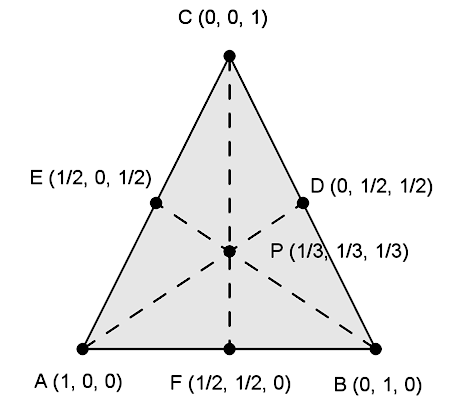
\includegraphics[scale=0.3]{Images/barycentric.png}
    \caption{Barycentric coodrinates of a 2-simplex. Here, the simplex is $s=\langle A,B,C\rangle$ and the triples of numbers next to each point $\alpha\in |s|$ in this triangle correspond to the list of values $(\alpha(A),\alpha(B),\alpha(C))$. The values of $\alpha$ thus represent the proportions in which $A,B,C$ have to be ``mixed'' to get a point inside this geometric realization of the simplex.\label{fig. simplex}}
\end{figure}


In the future we write $|K|=|K|_c$ and call this space the \emph{geometric realization} of $K$. For a simplex $s$ we define the \emph{closed simplex} $|s|\subset |K|$ as $|s|=\{\alpha\in|K|\mid \alpha(e)\neq 0\Rightarrow e\in s\}$ and the \emph{open simplex} as $\langle s\rangle=\{\alpha\in |K|\mid \alpha(e)\neq 0\Leftrightarrow e\in s\}$. The \emph{combinatorial boundary} of $|s|$ is $\partial|s|=|s|\setminus\langle s\rangle$.

\begin{defn}[Standard simplices in $\bbR^k$]
    Let $x_0,\ldots,x_n$ be affinely independent (i.e.\ $\sum_i\alpha_i x_i=0$ and $\sum_i\alpha_i=0$ imply $\alpha_j=0$). Then the simplex spanned by them is \[\langle x_0,\ldots,x_n\rangle=\left\{\sum_i \alpha_i x_i\mid \alpha_i\geq 0,\sum_i \alpha_i=1\right\}.\]
\end{defn}
\begin{defn}
    If $K=(E,S)$ is a simplicial complex and $\{x_e\mid e\in E\}$ a set of points in $\bbR^k$, and if a map
    \[f:|K|\to \bbR^k,\quad \alpha\mapsto \sum_{e\in E}\alpha(e)x_e\]
    is an embedding (say, topological), then $f(|K|)$ is called a simplicial polyhedron in $\bbR^k$ of type $K$, or a polyhedral realization of $K$ in $\bbR^k$.
\end{defn}
\begin{defn}[Triangulation]\index{Triangulation}
    Let $X$ be a topological space. A triangulation of $X$ is a triple $(X,K,f)$ where $K$ is a simplicial complex $K$ such that there is a homeomorphism $f:X\to |K|$.
\end{defn}

It is known that all differentiable manifolds can be triangulated, and the triangulation can be chosen so that on each simplex it is a smooth embedding.

\begin{defn}[Simplicial homology]\index{Homology!simplicial}
    For a simplicial complex $K=(E,S)$ define the group $C^\Delta_p(K)$ of \emph{simplicial $p$-chains} as the free abelian group generated by the set of all $p$-simplices in $K$. That is, elements of $C^\Delta_p(K)$ are formal sums $\sum_{s} c_s s$, where $s$ runs over all $p$-simplices in $K$, and only a finite number of coefficients $c_s\in \bbZ$ are nonzero at once.
    
    Define the \emph{boundary operator}\index{Boundary operator}
    \[\partial:\; C^\Delta_p(K)\to C^\Delta_{p-1}(K),\quad \partial\langle e_0,\ldots,e_p\rangle=\sum_{i=0}^p(-1)^p\langle e_0,\ldots,\wh{e}_i,\ldots,e_p\rangle,\]
    where the hat means skipping a vertex. It is easy to check that $\partial^2=0$, therefore we have the \emph{chain complex}\index{Complex!of simplicial chains}
    \[\cdots\to C^\Delta_2(K)\overset\partial\to C^\Delta_1(K)\overset\partial\to C^\Delta_0(K)\to 0.\]
    The group of $p$-cycles is $Z_p=\ker \restr{\partial}{C^\Delta_p(M)}$ and the group of $p$-boundaries is $B_p=\restr{\im\partial}{C^\Delta_{p+1}(M)}$. The \emph{simplicial homology groups} of $K$ are defined as
    \[H^\Delta_p(K)=Z_p/B_p.\]
\end{defn}

Intuitively, $H^\Delta_p$ detects the ``$p$-dimensional holes'' in the complex, because it consists of cycles that are not boundaries of anything $p+1$-dimensional.

\begin{defn}[Orientations on simplices and complexes]\index{Orientation!on simplicial complexes}
    An orientation on an $n$-simplex $s$ is an ordering of its elements into an $(n+1)$-tuple written as \[s=\langle e_0,\ldots,e_n\rangle.\]
    Orientations are considered to be equivalent if they differ by an even permutation of the vertices, i.e.\ we identify positively reordered tuples with each other. 
    
    In simplicial $p$-chains, sometimes the chain $-s$ is identified with $s$ oriented the opposite way.
    
    An orientation on a complex $K=(E,S)$ is a partial order on $E$ that induces an orientation on each simplex of $K$ (i.e.\ orientations of faces of a simplex can be induced from the orientation of the simplex). Orientations are considered to be equivalent if they induce equivalent orientations on all simplices.
\end{defn}

\begin{comment}
    \begin{samepage}
        \PRLsep
        \begin{center}
            {\red Lecture 21 on 10 May 2019 ended here (but Section \ref{finite dim de rham} was covered in the next lecture)}
        \end{center}
    \end{samepage}
\end{comment}

\begin{example}[Simplicial homology of $\bbS^1$]
    A circle $\bbS^1$ can be triangulated by a regular $n$-gon with vertices  $e_0,\ldots,e_{n-1}$ and oriented simplices $s_i=\langle e_i,e_{i+1}\rangle$, $0\leq i\leq n-1$ with the identification $e_n=e_0$. 
    Clearly 
    \[Z_0=C^\Delta_0=\bbZ^n,\quad C^\Delta_1=\left\{\sum_i c_i s_i \mid c_i\in \bbZ\right\}\cong \bbZ^n,\quad B_1=0.\]
    The chain complex is described by 
    \[\partial\langle e_i,e_{i+1}\rangle=\langle e_i\rangle-\langle e_{i+1}\rangle .\]
    $B_0$ consists of 0-chains $\sum c_i \langle e_i\rangle$ such that $\sum c_i=0$, thus $B_0\cong \bbZ^{n-1}$.
    Finally, $Z_1$ consists of 1-chains $\sum_i c_i s_i$ such that $c_i-c_{i+1}=0$ for all $i$, which means that $Z_1\cong \bbZ$ generated by the cycle $\sum_i s_i$. In the end, we have
    \[H^\Delta_0\cong \bbZ^n/\bbZ^{n-1}\cong \bbZ,\quad H^\Delta_1=Z_1\cong \bbZ. \]
    We notice that the ranks of these homology groups coincide with the dimensions of the corresponding de Rham cohomologies, see Example \ref{de Rham of circle}. We will later prove this as a general fact for all manifolds: the de Rham cohomology is isomorphic to the simplicial homology with real coefficients.
\end{example}


\begin{xca}
    If $K$ is the tetrahedron (with 2-dimensional faces included), i.e.\ a triangulation of $\bbS^2$, compute its homology groups:
    \[H^\Delta_0=\bbZ,\quad H^\Delta_1=0,\quad H^\Delta_2=\bbZ.\]
\end{xca}
\begin{xca}
    Triangulate the M\"obius band as in the figure.
    \begin{center}
        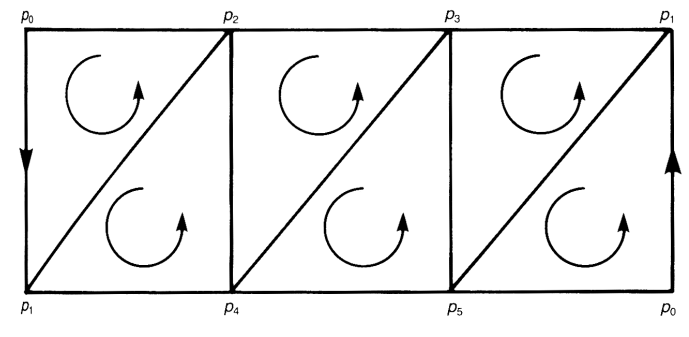
\includegraphics[scale=0.2]{Images/mobius.png}
    \end{center}
    Show that $H^\Delta_2(K)=0$ and $H^\Delta_1(K)=\bbZ$. In fact, the generator of $H^\Delta_1$ is the loop going from the bottom left to the top right corner in the diagram above.
\end{xca}

\begin{xca}
    Triangulate the real projective plane $\bbR P^2$ (which is homeomorphic to a disk whose antipodal boundary points have been identified) as in the figure.
    \begin{center}
        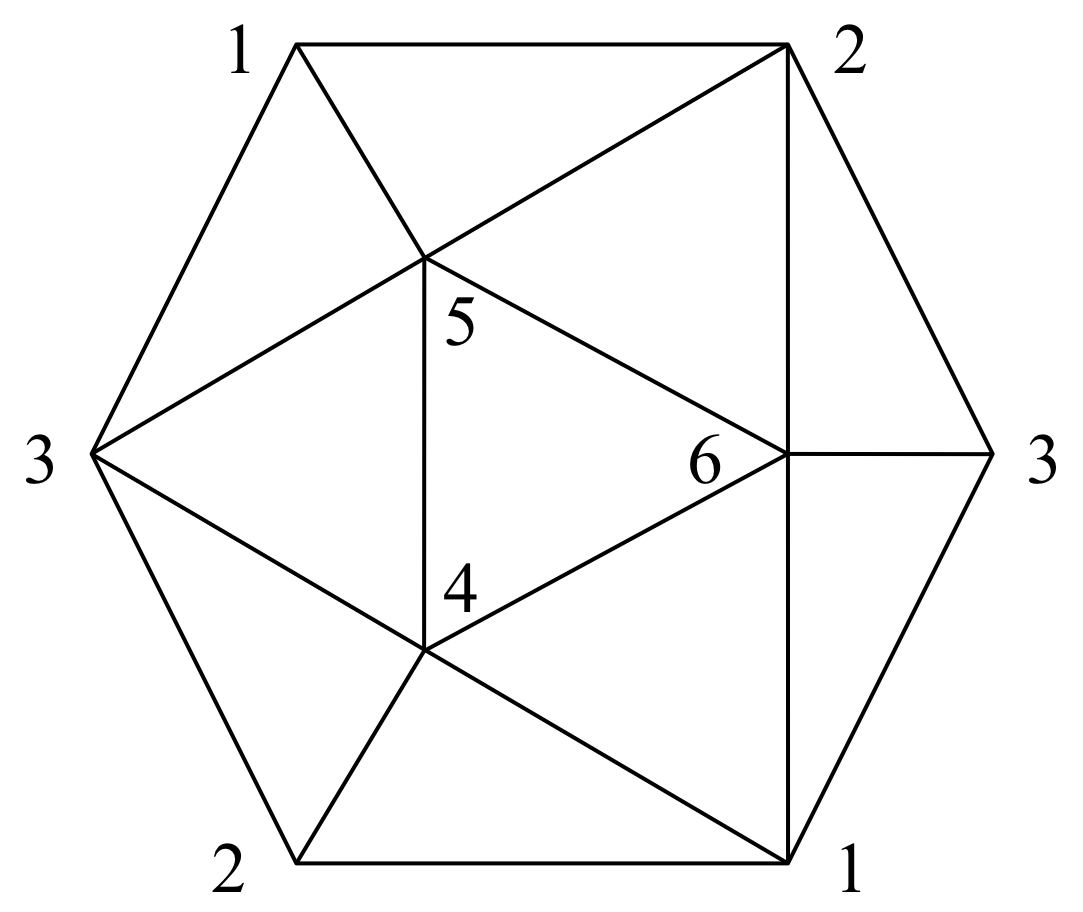
\includegraphics[scale=0.2]{Images/projectiveplane.png}
    \end{center}
    Show that $H^\Delta_2(K)=0$ and $H^\Delta_1(K)=\bbZ_2=\bbZ/2\bbZ$.
\end{xca}
\begin{xca}
    Triangulate the Klein bottle and show that $H^\Delta_1(K)=\bbZ\oplus\bbZ_2$.
\end{xca}

% \begin{defn}[Betti numbers]\index{Betti numbers}
%     Let $K$ be a finite simplicial complex. By the fundamental theorem of finitely generated abelian groups, each homology group of $K$ can be decomposed as
%     \[H_p(K)=\underbrace{\bbZ^{b_p(K)}}_{\text{free part}}\oplus \underbrace{\bbZ_{m_1}\oplus \cdots \oplus \bbZ_{m_k}}_{\text{torsion part}},\]
%     where $b_p(K)\geq 0$ are called \emph{Betti numbers}. 
%     Since the torsion part disappears when tensor multiplied by a field containing the rationals $\bbQ$ (the tensor product is understood to be over the ring $\bbZ$ because abelian groups are $\bbZ$-modules; then, say, $Z_m\otimes \bbQ$ consists of $a\otimes r=ma\otimes (r/m)=0$), we have
%     \[H_p(K)\otimes \bbQ=\bbQ^{b_p(K)}.\]
%     If $K$ is a triangulation of a smooth manifold $M$, then we will also show that $b_p(K)=\dim H_{\rm dR}^p(M)$.
% \end{defn}

% \begin{defn}[Euler characteristic]\index{Euler characteristic}
%     If $K$ is a finite $n$-dimensional simplicial complex, then there are two definitions of the Euler characteristic $\chi(K)$:
%     \begin{itemize}
%         \item $\chi(K)=\sum_{p=0}^n (-1)^p n_p(K)$, where $n_p(K)$ is the number of $p$-simplices in $K$ (``combinatorial Euler characteristic'');
%         \item $\chi(K)=\sum_{i=0}^n (-1)^p b_p(K)$, where $b_p(K)$ are the Betti numbers (``homological Euler characteristic'').
%     \end{itemize}
% \end{defn}

% \begin{thm}[Euler-Poincar\'e]
%     The two definitions of the Euler characteristic for finite simplicial complexes are equivalent. In particular, since the Betti numbers are homotopy invariants (because so is homology itself, which we will show later), so is the Euler characteristic.
% \end{thm}
% \begin{proof}
%     Consider chain groups with rational coefficients (i.e.\ the free parts of the usual groups),
%     \[C_p(K,\bbQ)\coloneqq C_p(K)\otimes\bbQ.\]
%     Now the boundary operator $\partial_p:C_p(K,\bbQ)\to C_{p-1}(K,\bbQ)$ is a linear operator on $\bbQ$-vector spaces and by the rank-nullity theorem
%     \[n_p(K)=\dim C_p(K,\bbQ)=\dim\ker\partial_p+\dim\im\partial_p.\]
%     On the other hand,
%     \[b_p(K)=\dim Z_p(K,\bbQ)/B_p(K,\bbQ)=\dim\ker\partial_p-\dim\im\partial_{p+1}.\]
%     When taking alternating sums of these over $p$, we will get the same answer in both cases.
% \end{proof}




\subsection{Homological algebra II: complexes}

\begin{defn}[(Co)chain complexes]\index{Complex!of chains}\index{Complex!of cochains}
    A chain complex $(\bm{C},d)$ in an abelian category $\calC$ is a sequence  of morphisms 
    \[\cdots\to C_{n+1}\overset{d_{n+1}}\to C_n\overset{d_n}\to C_{n-1}\to\cdots\]
    indexed by $n\in \bbZ$, such that $d_n\circ d_{n+1}=0$.
    
    Similarly, a cochain complex is a sequence
    \[\cdots\to C^{n-1}\overset{d^{n-1}}\to C^n\overset{d^n}\to C^{n+1}\to\cdots\]
    such that $d^{n+1}\circ d^n=0$.
\end{defn}

Note that there is no actual difference between chain and cochain complexes, since simply changing the enumeration $n\mapsto -n$ turns one into the other. Therefore all general results need to be proven only for chain complexes.

\begin{defn}[(Co)cycles, (co)boundaries, (co)homologies of complexes]\index{Homology!of a chain complex}\index{Cohomology!of a cochain complex}
    For a chain complex $(\bm{C},d)$, $n$-cycles, $n$-boundaries, and homologies are defined as 
    \[Z_n(\bm{C},d)=\ker d_n,\quad\quad B_n(\bm{C},d)=\im d_{n+1},\quad\quad H_n(\bm{C},d)=Z_n(\bm{C},d)/B_n(\bm{C},d).\]
    
    Similarly, for a cochain complex $(C^\bullet,d)$, we have cocycles, coboundaries, and cohomologies:
    \[Z^n(C^\bullet,d)=\ker d_n,\quad\quad B^n(C^\bullet,d)=\im d^{n-1},\quad\quad H^n(C^\bullet,d)=Z^n(C^\bullet,d)/B^n(C^\bullet,d).\]
\end{defn}

\begin{defn}[Chain map]
    If $(\bm{B},\delta )$ and $(\bm{C},d)$ are two chain complexes, then a chain map $f:\bm{B}\to \bm{C}$ is a sequence of maps $f_n:B_n\to C_n$ such that $d_n\circ f_n=f_{n-1}\circ \delta_n$, i.e.\ such that the full diagram commutes:
    \[\begin{tikzcd}[every matrix/.append style={name=m},
        execute at end picture={\draw [<-] ([xshift=-8mm,yshift=-10mm]m-1-3.north) arc[start angle=-90,delta angle=-270,radius=0.2cm];
        \draw [<-] ([xshift=-8mm,yshift=-10mm]m-1-4.north) arc[start angle=-90,delta angle=-270,radius=0.2cm];}]
        \cdots\arrow[r] & B_{n+1}\arrow[r]\arrow[d,swap,"f_{n+1}"] & B_{n} \arrow[r]\arrow[d,swap,"f_n"] & B_{n-1}\arrow[d,"f_{n-1}"]\arrow[r] & \cdots \\
       \cdots\arrow[r] & C_{n+1}\arrow[r] & C_n\arrow[r] &C_{n-1} \arrow[r] &\cdots
    \end{tikzcd}\]
    Similarly one defines cochain maps between cochain complexes.
\end{defn}

\begin{prop}
    All chain complexes in an abelian category $\calC$ with chain maps between them comprise an abelian category called $\mathsf{Comp}(\calC)$.
\end{prop}
\begin{proof}
    By the Freyd-Mitchell theorem, we only need to prove this for $\calC=R\text{-}\mathsf{Mod}$. For such a category it is obvious what the structure of an abelian category on complexes is: the zero object is the zero complex; direct sums are defined by summing in each degree; the kernel and cokernel of $f$ are the complexes consisting of $\ker f_n$ and $\coker f_n$; images and coimages coincide because they do so in $\calC$.
\end{proof}

\begin{defn}[Positive complexes]
    A chain complex $\bm{C}$ is called positive if $C_n=0,n<0$. All positive complexes form the full subcategory $\mathsf{Comp}_{\geq 0} (\calC)$ of $\mathsf{Comp}(\calC)$:
    \[\cdots\to C_n\to C_{n-1}\to\cdots\to \to C_1\to C_0\to 0.\]
    
    A negative chain complex
    \[0\to C_0\to C_{-1}\to \cdots \to C_{-n}\to C_{-n-1}\to\cdots\]
    is identified with a positive cochain complex 
    \[0\to C^0\to C^{1}\to \cdots \to C^{n}\to C^{n+1}\to\cdots\]
    by setting $C^n=C_{-n}$ and $d^n=d_{-n}$.
\end{defn}

\begin{prop}
    If $\calC$ is an abelian category, then the $n$-th homology $H_n:\mathsf{Comp}(\calC)\to \calC$ is an additive (covariant) functor for all $n\in \bbZ$.
\end{prop}
\begin{proof}
    Given a chain map $f:\bm{A}t\to \bm{B}$, we need to construct a morphism $H_n(f):H_n(\bm{A})\to H_n(\bm{B})$. Since $H_n(\bm{A})=Z_n(\bm{A})/B_n(\bm{A})$, we can try to take a $z$ such that
    \[f_n:Z_n(\bm{A})\to B_n,\quad z\mapsto f_n(z)\]
    and define
    \[H_n(f):H_n(\bm{A})\to H_n(\bm{B}),\quad [z]\to \left[f_n(z)\right],\]
    where equivalence classes are taken w.r.t.\ to the quotients by $B_n(\bm{A})$ and $B_n(\bm{B})$ respectively.
    
    First we need to check that $f_n(z)\in Z_n(\bm{B})$. We will use the same symbol $d_n$ for morphisms in both complexes. By the definition of a chain map, $d_n(f_n(z))=f_{n-1}(d_n(z))=0$ since $z\in B_n(\bm{A})$.
    
    Next we need to check correctness, i.e.\ independence of $H_n(f)([z])$ of the choice of representative. Let $z,z'\in Z_n(\bm{A}):[z]=[z']\Leftrightarrow z-z'\in B_n(\bm{A})$, then
    \[\exists y\in A_{n+1}: d_{n+1}(y)=z-z'\implies d_{n+1}(f_{n+1}(y))=f_n(z)-f_n(z'),\]
    which means that $f_n(z)-f_n(z')$ is a boundary, proving what we wanted.
    
    To check functoriality, say we have two chain maps
    \[\bm{A}\overset f\to \bm{B}\overset g\to \bm{C}.\]
    We need to show the commutativity of the triangle
    \[
    \begin{tikzcd}
        H_n(\bm{A}) \arrow[rr,"H_n(f)"]\arrow[dr,swap,"H_n(g\circ f)"]&& H_n(\bm{B})\arrow[dl,"H_n(g)"]\\
        & H_n(\bm{C}) &
    \end{tikzcd}
    \]
    We have 
    \begin{multline}
        H_n(g\circ f)([z])=\left[(g\circ f)_n(z)\right]=\left[g_n\circ f_n(z)\right]=H_n(g)\left(\left[f_n(z)\right]\right)=\\=H_n(g)\left(H_n(f)[z]\right)=H_n(g)H_n(f)([z]).
    \end{multline}
    
    Finally, additivity is trivial since $f_n$ are homomorphisms:
    \[H_n(f+f')=H_n(f)+H_n(g').\]
\end{proof}

\begin{rem}
    On cochain complexes, this functor is of course contravariant.
\end{rem}

From now on we write
\[f_\ast=H_n(f),\quad\quad g^\ast=H^n(g)\]
for the descendants of maps in (co)homology.

\begin{lem}
    Exact additive covariant functors preserve homology: $H_\ast(F(\bm{C}))\cong F(H_\ast(\bm{C}))$.
\end{lem}
\begin{proof}
    This follows from the fact that exact additive functors preserve kernels and quotients (and all functors preserve images).
\end{proof}

\begin{prop}
    The direct limit of the homology groups of a directed system of chain complexes $\bm{C}^i$ is the homology group  of the direct limit:
    \[\colimit_i H_n(\bm{C}^i)\cong H_n(\colimit_i \bm{C}^i).\]
\end{prop}
\begin{proof}
    This follows immediately from the preceding Lemma and the fact that direct limits preserve exactness in abelian categories (Proposition~\ref{prop direct limits preserve exactness}).
\end{proof}
\begin{rem}
    Note that the analogous statement for homotopy groups $\pi_n$ was proven by us only for sequences of $CW$ subcomplexes (Corollary~\ref{cor direct limit of pi_n for CW}) and does not hold in general even for $\pi_1$.
\end{rem}



\begin{thm}[Connecting homomorphism lemma]\label{connecting hom in homology}
    Let 
    \[0\to \bm{A}\overset i\to \bm{B}\overset\pi\to \bm{C}\to 0 \]
    be a short exact sequence of chain complexes. Then for each $n$ there is a \emph{connecting homomorphism}
    \[\delta=\delta_n:H_n(\bm{C})\to H_{n-1}(\bm{A}),\quad [z]\to \left[i_{n-1}^{-1} d_n\pi_n^{-1}(z)\right].\]
\end{thm}
\begin{proof}
    Several checks need to be done. First, why does $d_n\pi_n^{-1}(z)\in\im i_{n-1}$? Let $y:\pi_n(y)=z$, then $d_n(y)\in B_{n-1}$. Since $z\in Z_n(\bm{C})$ we have $\pi_{n-1}(d_n(y))=d_n(\pi_n(y))=d_n(z)=0$. Therefore $\exists ! x\in A_{n-1}:i_{n-1}(x)=d_n(y)$, and we have a well defined map
    \[z\mapsto x.\]
    
    Next, we need to verify that $d_{n-1}(x)=0$ and the class $[x]\in H_{n-1}(\bm{A})$ is independent of the choice of $y$.
    Moreover, one needs to check that if $[z]=[z']$, then $[x]=[x']$. Lastly, we need to check that $\delta$ is a homomorphism. These checks are left as an exercise.
\end{proof}

\begin{thm}[Zig-zag lemma/Long exact sequence in homology]\label{thm long exact seq in homology}
    For any short exact sequence of complexes 
    \[0\to \bm{A}\overset i\to \bm{B}\overset\pi\to \bm{C}\to 0 ,\]
    the induced sequence in homology
    \[\cdots \to H_{n+1}(\bm{C})\overset{\delta_{n+1}}\to H_n(\bm{A})\overset{i_\ast}\to H_n(\bm{B})\overset{\pi_\ast}\to H_n(\bm{C})\overset{\delta_n}\to H_{n-1}(\bm{A})\to \cdots \]
    is exact.
\end{thm}
\begin{proof}
    It is easy to see that for any complex $\bm{C}$ the two \emph{``fundamental sequences''}
    \[0\to Z_n(\bm{C})\to C_n\overset{d_n}\to B_{n-1}(\bm{C})\to 0,\]
    \[0\to B_n(\bm{C})\to Z_n(\bm{C})\to H_n(\bm{C})\to 0\]
    are short exact.
    This one is also obviously exact:
    \[0\to B_n(\bm{C})\to C_n\to C_n/B_n(\bm{C})\to 0.\]
    Using the exactness of the first sequence, we also have the exactness of this one:
    \[0\to H_n(\bm{C})\to C_n/B_n(\bm{C})\to \underbrace{B_{n-1}(\bm{C})}_{\cong C_n/Z_n(\bm{C})}\to 0.\]
    
    Putting it all together, we conclude the exactness of this sequence:
    \[0\to H_n(\bm{C})\to C_n/B_n(\bm{C})\to Z_{n-1}(\bm{C})\to H_{n-1}(\bm{C})\to 0.\]
    Now let us use this sequence for the columns of one large diagram:
    \[\begin{tikzcd}
        && 0\ar{d}& 0\ar{d} &0\ar{d} &&\\
        & & H_n(\bm{A}) \ar{r} \ar{d} & H_n(\bm{B})\ar{r} \ar{d} &  H_n(\bm{C}) \ar{d}   %\arrow[ddll,"\delta",rounded corners
        & & \\
        &  &  A_n/B_n(\bm{A}) \ar{r} & B_n/B_n(\bm{B}) \ar{r} \ar{dd} &  C_n/B_n(\bm{C})\ar{r}\ar{dd} & 0 &  ~\\[-10pt]
        & & &  ~ & & \ar[r, phantom, ""{coordinate, name=Y}] & ~\\[-10pt]
        ~&  \ar[l, phantom, ""{coordinate, name=Z}] 0 \ar{r} &  Z_{n-1}(\bm{A}) \ar[uu,leftarrow,crossing over]\ar{r} \ar{d} &  Z_{n-1}(\bm{B}) \ar{r} \ar{d} &  Z_{n-1}(\bm{C}) \ar{d} & &  \\
              & &  \ar[from=uuuurr, "\delta_n", dashed,crossing over, rounded corners,
                      to path=
                              { -- ([xshift=2ex]\tikztostart.east)
                              -| (Y) [near end]\tikztonodes
                              -| (Z) [near end]\tikztonodes
                              |- ([xshift=-2ex]\tikztotarget.west)
                               -- (\tikztotarget)}
                    ] H_{n-1}(\bm{A})\ar{r}\ar{d}
               &  H_{n-1}(\bm{B}) \ar{r}\ar{d}
               &  H_{n-1}(\bm{C})\ar{d}
               & 
               & \\
        && 0& 0 &0 &&\\
    \end{tikzcd}\]
    The exactness of the rows can be checked directly using the exactness of $\bm{A}\to \bm{B}\to\bm{C}$. Then this is in fact exactly the type of diagram for which we can apply the Snake Lemma \ref{snake lemma} and establish the existence of $\delta_n$. It only remains to check that the construction of $\delta_n$ in the Snake Lemma exactly coincides with the one in Proposition \ref{connecting hom in homology}.
\end{proof}
\begin{cor}
    The Snake lemma is equivalent to the Zig-zag lemma.
\end{cor}
\begin{proof}
     The proof of Theorem \ref{thm long exact seq in homology} shows that the Snake Lemma implies the long exact sequence in homology. The converse also trivially holds since we can apply the Zig-zag lemma to a short exact sequence of complexes concentrated in just two degrees of the form $0\to \ker\pi \to \im\pi \to 0$ (let the two other complexes have $\rho $ and $\sigma$ instead of $\pi$) and obtain the long exact sequence of homologies, which reads
    \[0\to \ker\pi \to \ker\rho\to \ker\sigma\to \coker\pi\to \coker\rho\to\coker\sigma\to 0, \]
    which is exactly the Snake Lemma \ref{snake lemma}.
\end{proof}

\begin{comment}
    \begin{samepage}
        \PRLsep
        \begin{center}
            {\red Lecture 22 on 17 May 2019 ended here (included Section \ref{finite dim de rham})}
        \end{center}
    \end{samepage}
\end{comment}


\begin{prop}[Naturality of the connecting homomorphism\tablefootnote{Tape worm lemma?}]\label{naturality of connecting hom}
    Given a commutative diagram with exact rows in the category $\mathsf{Comp}(\calC)$
    \[\begin{tikzcd}
        0\arrow[r] & \bm{A}\arrow[r,"i"]\arrow[d,swap,"f"] & \bm{B} \arrow[r,"p"]\arrow[d,swap,"g"] & \bm{C}\arrow[d,"h"]\arrow[r] & 0 \\
       0\arrow[r] & \bm{A}'\arrow[r,"j"] & \bm{B}'\arrow[r,"q"] &\bm{C}' \arrow[r] &0
    \end{tikzcd}\]
    there is a commutative diagram in $\calC$ with exact rows
    \[\begin{tikzcd}
        ~\arrow[r]& H_n(\bm{A})\arrow[r,"i_\ast"]\arrow[d,"f_\ast"] & H_n(\bm{B}) \arrow[r,"p_\ast"]\arrow[d,"g_\ast"] & H_n(\bm{C})\arrow[d,"h_\ast"]\arrow[r,"\delta"] & H_{n-1}(\bm{A})\arrow[d,"f_\ast"]\arrow[r]&~ \\
       ~\arrow[r] & H_n(\bm{A}')\arrow[r,"j_\ast"] & H_n(\bm{B}')\arrow[r,"q_\ast"] &H_n(\bm{C}') \arrow[r,"\delta'"] &H_{n-1}(\bm{A}')\arrow[r]&~ 
    \end{tikzcd}\]
    In other words, morphisms between exact sequences of complexes naturally induce morphisms between the exact sequences in homology, i.e.\ the connecting homomorphism $\delta$ is natural w.r.t.\ such morphisms.
\end{prop}
\begin{proof}
     The exactness of the rows is the content of the theorem about the long exact sequence. The commutativity of the first two squares follows from the functoriality of $H_n$. Checking the commutativity of the square $\delta'\circ h_\ast=f_\ast\circ \delta$ requires expanding the first commutative diagram in $\mathsf{Comp}(\calC)$ into a 3-dimensional diagram in $\calC$.
     \[
     \begin{tikzcd}[column sep={35,between origins}]
        &
        0 
        \ar{rr}
        & &
        A_n
        \ar{dl}[swap, sloped, near start]{d}
        \ar{rr}{i}
        \ar[]{dd}[near start]{f_\ast}
        & & B_n
        \ar{dd}[near start]{g_\ast}
        \ar{rr}{p}
        \ar{dl}[swap, sloped, near start]{d}
        & & C_n
        \ar{dd}[near start]{h_\ast}
        \ar{dl}[swap, sloped, near start]{d}
        \ar{rr}
        & &
        0
        \\
        0
        \ar{rr}
        & &
        A_{n-1}
        \ar[crossing over]{rr}[near end]{i}
        & & B_{n-1}
        \ar[crossing over]{rr}[near end]{p}
        & & C_{n-1}
        \ar[crossing over]{rr}
        & &
        0
        \\
        &
        0
        \ar{rr}
        & &
        A_n'
        \ar[near start]{rr}{j}
        \ar[sloped, swap]{dl}{d}
        & & B_n'
        \ar[near start]{rr}{q}
        \ar[sloped, swap]{dl}{d}
        & & C_n'
        \ar[sloped, swap]{dl}{d}
        \ar{rr}
        & &
        0
        \\
        0
        \ar{rr}
        & &
        A_{n-1}'
        \ar{rr}{j}
        \ar[crossing over, leftarrow, near start]{uu}{f_\ast}
        & & B_{n-1}'
        \ar{rr}{q}
        \ar[crossing over, leftarrow, near start]{uu}{g_\ast}
        & & C_n'
        \ar[crossing over, leftarrow, near start]{uu}{h_\ast}
        \ar{rr}
        & &
        0
        \end{tikzcd}
     \]
     Taking $[c]\in H_n(\bm{C})$, we must show that $f_\ast\delta [c]=\delta ' h_\ast [c]$. Let $b\in B_n$ be such that $p(b)=c$. Then $\delta [c]=[a]$, where $i(a)=d(b)$. Hence $f_\ast \delta [c]=[f(a)]$. 
     
     On the other hand, since $h$ is a chain map, $q(g(b))=h(p(b))=h(c)$. Hence we can use $g(b)$ as the pre-image of $h(c)$ in $B_n'$, so by construction of the connecting homomorphism, $\delta '[h(c)]=[a']$ where $j(a')=d(g(b))$. But $j(f(a))=g(i(a))=g(d(b))=d(g(b))=j(a')$ and so $f(a)=a'$ because $j$ is injective. Therefore $\delta'h_\ast [c]=[a']=[f(a)]$, which coincides with the l.h.s.\ computed above.
\end{proof}

Naturality is instrumental in many arguments involving long exact sequences because it means that we can apply sequences of chain maps to long exact sequences and preserve the commutativity of diagrams.

\begin{prop}[Algebraic Mayer-Vietoris sequence]\label{prop algebraic MV}
    If in the setting of Theorem \ref{naturality of connecting hom}, $h_\ast$ is also an isomorphism in homology, then one has the long exact sequence
    \[\cdots \to H_{n+1}(\bm{B}')\overset\Delta\to H_n(\bm{A})\overset{(f_\ast,i_\ast)}\longrightarrow H_n(\bm{A}')\oplus H_n(\bm{B})\overset{j_\ast- g_\ast}\longrightarrow H_n(\bm{B}')\overset{\Delta}\to H_{n-1}(\bm{A})\to \cdots\]
    where $\Delta=\delta \circ h_\ast^{-1}\circ q_\ast$.
\end{prop}
\begin{proof}
     This is an exercise in diagram chasing.
\end{proof}

The relation of this Proposition to the \gls{mv} sequence in de Rham cohomology will become clear when we get to relative (co)homology and the excision property. The isomorphism $h_\ast$ in question is $H_n(U,U\cap V)\cong H_n(M,V)$ for $M=U\cup V$. A rough visualization of $H_n(X,Y)$ with $Y\subset X$ is the homology of the space obtained from $X$ by contracting $Y$ into one point. Then it is clear that contracting $V$ inside $M$ has the ``same'' result as contracting $U\cap V$ inside $U$. 


\begin{defn}[Maps of degree $p$]
    Let $\bm{C}$ and $\bm{D}$ be two chain complexes in $\calC$. A map of degree $p$ between them, denoted $s:\bm{C}\to \bm{D}$, is a collection of maps $s_n:C_n\to D_{n+p}$. Note that no commutativity is required here!
\end{defn}


Now that we know that $H_n$ is a functor, it is natural to ask how much $H_n(f)$ actually depends on $f$. It turns out that $H_n(f)$ is invariant under homotopies of $f$ defined in the following categorical sense.


\begin{defn}
    Let $f,g:\bm{B}\to \bm{C}$ be two chain maps. They are called homotopic ($f\sim g$) if there is a map of degree $+1$ denoted $s:\bm{B}\to \bm{C}$ such that 
    \[\forall n,\quad f_n-g_n=d_{n+1}s_n+s_{n-1}d_n.\]
    (As usual, we use $d_n$ to denote the differentials in all complexes at once).
    This can be visualized by the following \emph{non-commutative} diagram:
     \[\begin{tikzcd}
        \cdots\ar[r] & B_{n+1}\ar[r]\ar[dd,swap, xshift=-.75ex,"f_{n+1}"]\ar[dd,xshift=.75ex,"g_{n+1}"] & B_{n} \arrow[r]\ar[dd,swap,xshift=-.75ex,"f_n"]\ar[dd,xshift=.75ex,"g_n"]\ar[ddl,sloped, near start,"s_n"] & B_{n-1}\ar[dd,swap,xshift=-.75ex,"f_{n-1}"]\ar[dd,xshift=.75ex,"g_{n-1}"]\ar[r]\ar[ddl, near start,sloped,"s_{n-1}"] & \cdots \\
        &&&&\\
       \cdots\ar[r] & C_{n+1}\ar[r] & C_n\ar[r] &C_{n-1} \ar[r] &\cdots
    \end{tikzcd}\]
\end{defn}

\begin{thm}
    Homotopic chain maps induce the same morphism in homology.
\end{thm}
\begin{proof}
     Let $s:\bm{B}\to\bm{C}$ be the homotopy. If $z$ is an $n$-cycle, dropping subscripts, $d z=0$, then
     \[f(z)-g(z)=d(s(z))+s(d(z))=d(s(z)),\]
     i.e.\ $f(z)-g(z)\in B_n(\bm{C})$ and $f_\ast=g_\ast$.
\end{proof}

\begin{defn}[Acyclic, contractible complexes]\index{Acyclic complex}\index{Contractible complex}
    A complex is called acyclic if all its (co)homologies are trivial. A complex $\bm{C}$ is called contractible if there exists a homotopy $1_{\bm{C}}\sim 0_{\bm{C}}$. 
    All contractible complexes are acyclic since contractibility implies $1_{H_n(\bm{C})}=0_{H_n(\bm{C})}$.
\end{defn}

\begin{defn}[Quasi-isomorphisms]\index{Quasi-isomorphism}
    Two complexes $\bm{A},\bm{B}$ are called quasi-isomorphic (or \emph{weakly equivalent}) if there is a chain map $f:\bm{A}\to \bm{B}$ such that $f_\ast=H_n(f):H_n(\bm{A})\to H_n(\bm{B})$ is an isomorphism for all $n$.
\end{defn}

\begin{defn}[Homotopy equivalence]\index{Homotopy equivalence}
    Two complexes $\bm{A},\bm{B}$ are called homotopy equivalent if there are two chain maps $f:\bm{A}\to \bm{B}$ and $g:\bm{B}\to\bm{A}$ such that
    \[f\circ g\sim 1_{\bm{B}},\quad g\circ f\sim 1_{\bm{A}}.\]
    Clearly homotopy equivalent complexes are quasi-isomorphic.
\end{defn}


\begin{xca}\label{Lie derivative homotopy operator}
    Check that a Lie derivative $\Lie_X$ is a cochain map on the de Rham complex. Furthermore, show that applying a Lie derivative $\Lie_X$ to a differential form doesn't change its class in de Rham cohomology. For this, find the homotopy operator between $\Lie_X$ and the zero morphism.
\end{xca}







\subsection{Singular homology}

de Rham cohomology is defined only for smooth manifolds, and simplicial homology is defined only for triangulable spaces. The type of homology we define now works for all topological spaces, but proving its properties for nicer spaces (like manifolds) requires extra work. The idea is, instead of trying to break up our topological space into simplices, to study the set of all continuous maps from simplices to our space.

\begin{defn}[Singular simplices]\index{Simplex!singular}
    We denote by $\Delta^n$ the standard $n$-simplex $\Delta^n=\{\sum_{i=0}^{n} \alpha_i e_i\mid \sum_i\alpha_i=1\}$, where $\{e_i\}_{i=0}^{n}$ is the standard basis in $\bbR^{n+1}$. Let $X$ be a topological space. A singular $n$-simplex in $X$ is a continuous map $\sigma\in C(\Delta^n, X)$ (no other constraints, hence ``singular''). The group $C_n(X)$ of singular $n$-chains is the free abelian group generated by the set $C(\Delta^n,X)$. Sometimes we will write $C^{\text{sing}}_n(X)$ to distinguish from other kinds of chain groups.
\end{defn}
\begin{defn}[Singular homology]\index{Homology!singular}
    The boundary map $\partial_n:C_n(X)\to C_{n-1}(X)$ is defined as before:
    \[\partial_n\sigma=\sum_i (-1)^i\restr{\sigma}{\langle e_0,\ldots,\wh{e}_i,\ldots,e_n\rangle},\]
    where we implicitly identify the faces of $\Delta^n$ with $\Delta^{n-1}$ while preserving the order of vertices, so that $\restr{\sigma}{\langle e_0,\ldots,\wh{e}_i,\ldots,e_n\rangle}$ is a singular $(n-1)$-simplex.
    
    Singular homology groups are defined as
    \[H_n(X)=\ker\partial_n/\im\partial_{n+1}.\]
\end{defn}

Unlike with simplicial homology, here it is immediately obvious that homeomorphic spaces have isomorphic singular homologies. The price we pay for this is that the rank of $C^{\text{sing}}_n(X)$ is uncountably large, so it is not clear at a glance whether singular homologies of spaces that have finitely generated simplicial homologies are also finitely generated. 

\begin{prop}
    If $X$ consists of $l$ path-connected components, then $H_0(X)\cong \bbZ^l$.
\end{prop}
\begin{proof}
     It suffices to prove this for $l=1$, i.e.\ a path-connected $X$. We have $H_0(X)=C_0(X)/\im\partial_1$. A singular 0-chain in $X$ is just a finite sum $\sum_i n_i p_i$ where $p_i$ are points in $X$ and $n_i\in\bbZ$. Define the homomorphism $\epsilon:C_0(X)\to \bbZ$, called the \emph{augmentation map}\index{Augmentation map}, by
     \[\epsilon\left(\sum_i n_i p_i\right)=\sum_i n_i.\]
     It is surjective as long as $X\neq\varnothing$. The claim is that $\ker\epsilon\cong\im\partial_1$ if $X$ is path-connected, so $\epsilon $ induces an isomorphism $H_0(X)\cong \bbZ$.
     
     First, it is clear by definition of $\partial$ that $\im\partial_1\subset\ker\epsilon$. For the reverse inclusion, suppose $\epsilon(\sum_i n_i p_i)=0$. Choose a path $\gamma_i$ connecting a base point $x_0$ to $p_i$. We can view $\gamma_i$ as a singular 1-simplex and have $\partial\gamma_i=p_i-x_0$. Hence $\partial(\sum_i n_i\gamma_i)=\sum_i n_i p_i$ since $\sum_i n_i=0$. Therefore $\sum n_i p_i$ is a boundary, which shows $\ker\epsilon\subset\im\partial_1$.
\end{proof}

\begin{prop}
    If $X$ consists of a single point, then $H_n(X)=0$ for $n>0$ and $H_0(X)\cong \bbZ$.
\end{prop}
\begin{proof}
     In this case there is a unique singular $n$-simplex $\sigma_n$ for each $n$ and 
     \[\partial\sigma_n=\sum_{i=0}^n(-1)^i\sigma_{n-1}=\begin{cases}
     0,& n\text{ odd},\\
     \sigma_{n-1},& n\text{ even}.
     \end{cases}\]
     This the singular chain complex reads
     \[\cdots\to \bbZ\overset\cong\to \bbZ\overset 0\to \bbZ\overset\cong\to\bbZ\overset 0\to\bbZ\to 0.\]
     The homology of this complex is trivial except for $H_0\cong \bbZ $.
\end{proof}

Sometimes it is very helpful to work with a slightly modified homology that vanishes entirely for a point. The following definition achieves this.

\begin{defn}[Reduced homology]\index{Homology!reduced}
    The reduced homology groups $\wt{H}_n(X)$ are the homology groups of the \emph{augmented chain complex}
    \[\cdots C_1(X)\overset{\partial_1}\to C_0(X)\overset{\epsilon}\to \bbZ\to 0.\]
\end{defn}

The reduced homology of a point is trivial in all degrees. Also $H_n(X)\cong \wt{H}_n(X)$ for all $n>0$ and $H_0(X)=\wt{H}_0(X)\oplus \bbZ$ since $\epsilon$ induces a map $H_0(X)\to \bbZ$ with kernel $\wt{H}_0(X)$.




\subsection{Homotopy invariance}

Here we show that singular homology is homotopy invariant.


\begin{prop}[{{\cite[Thm. 2.10]{Hatcher}}}]\label{thm 2.10 Hatcher}
    If two maps $f,g\in C(X,Y)$ between topological spaces $X,Y$ are homotopic, then they induce the same homomorphism in homology
    \[f_\ast=g_\ast :H_n(X)\to H_n(Y)\]
    for all $n$. In particular, homotopy equivalent spaces have isomorphic homology groups.
\end{prop}
\begin{wrapfigure}[10]{r}{0.2\textwidth}
    \begin{center}
        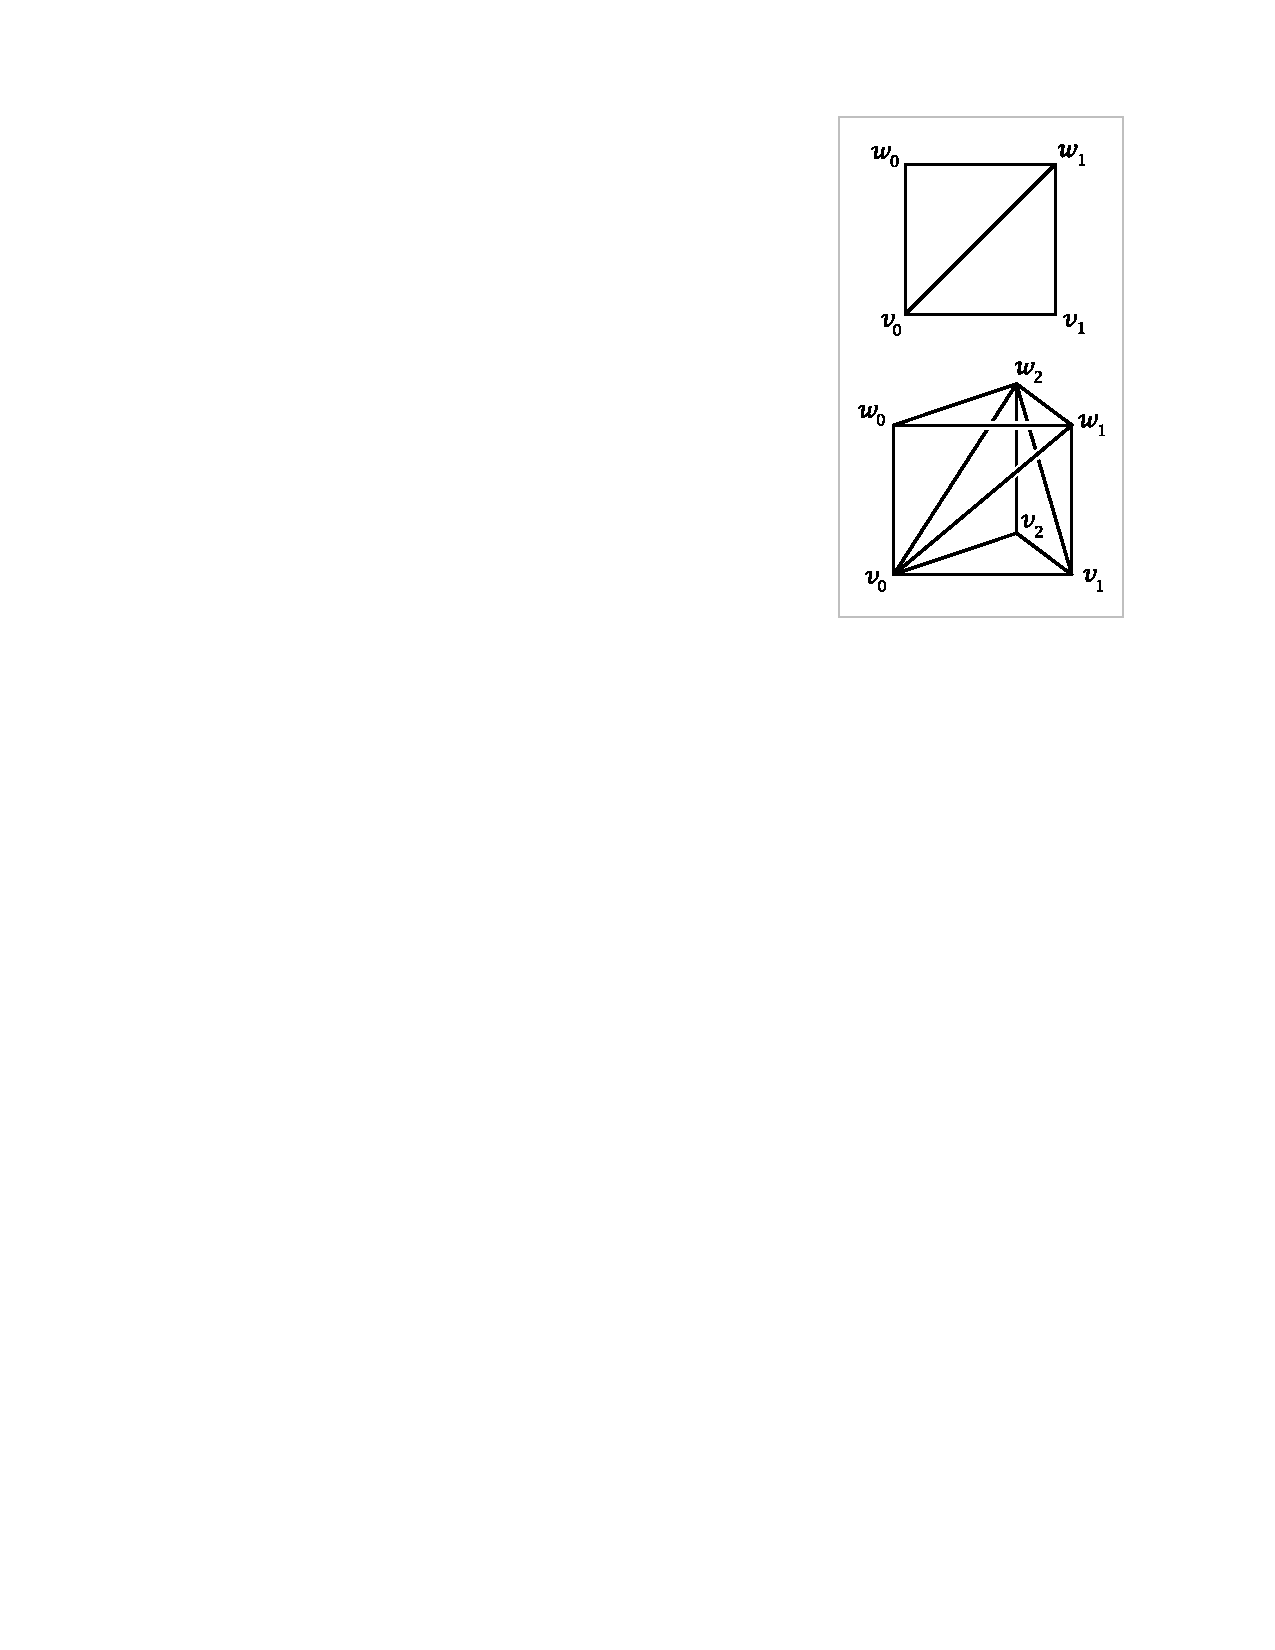
\includegraphics[width=0.2\textwidth]{Images/prism.pdf}
    \end{center}
    \caption{Triangulation of a prism.\label{Prism fig}}
\end{wrapfigure}
\begin{proof}
     The key is learning to subdivide the prism $\Delta^n\times I$ (where $I=[0,1]$) into simplices. If $\langle v_0,\ldots,v_n\rangle$ is the copy of $\Delta^n$ at the bottom of the prism and $\langle w_0,\ldots,w_n\rangle$ is the one at the top, then it is easy to check that the prism is triangulated by the $(n+1)$-simplices $\langle v_0,\ldots,v_i,w_i,\ldots,w_n\rangle$, each intersecting the next in an $n$-simplex face. The cases $n=1,2$ are shown in figure~\ref{Prism fig}.
     
     Given a homotopy $F:X\times I\to Y$ from $f$ to $g$ and a singular simplex $\sigma:\Delta^n\to X$, we form the composition $F\circ(\sigma\times \id):\Delta^n\times I\to X\times I\to Y$. Using this, we define the \emph{prism operators}
     \[P:C_n(X)\to C_{n+1}(Y),\quad P(\sigma)=\sum_i(-1)^i F\circ (\sigma\times\id)\langle x_0,\ldots,v_i,w_i,\ldots,w_n\rangle.\]
     We claim that $P$ is a homotopy operator between these two chain complexes, namely
     \[g_\ast-f_\ast=\partial P+P\partial.\]
     The geometric meaning of $\partial P=g_\ast-f_\ast-P\partial$ is that the boundary of the prism equals its top $\Delta^n\times\{1\}$, minus its bottom $\Delta^n\times\{0\}$, and plus the sides $\partial\Delta^n\times I$ (compare this with Cartan's magic formula and its cohomological meaning, which is nothing but a dual to this geometric statement, see Exercise~\ref{Lie derivative homotopy operator}).
     
     The verification of this identity follows easily by direct expansion and use of the definition of the homotopy $F$ and $g\circ\sigma=g_\ast(\sigma)$ (see \cite[Thm.~2.10]{Hatcher} for full details).
\end{proof}
\begin{cor}
    If $X$ is contractible, then $\wt{H}_n(X)=0$ for any $n$.
\end{cor}


Continuous maps induce homomorphisms in reduced homology as well since the augmentation map $\epsilon$ commutes with $f_\ast$. Then the same theorem holds for reduced homologies with the same proof.




\subsection{Relative homology and excision}

Relative homology generalizes the idea behind the \gls{mv} sequence in de Rham cohomology. Given a subset $A\subset X$ in a topological space, we ask how similar the groups $H_n(X/A)$ and $H_n(X)/H_n(A)$ are. The difference, in a sense, is measured by the relative homology.

\begin{defn}
    Let $X$ be a topological space and $A\subset X$ a topological subspace (i.e.\ a subset with the induced subset topology). The group of singular chains $C_n(A)$ can be treated as a subgroup of $C_n(X)$. Define the relative singular chain groups as $C_n(X,A)=C_n(X)/C_n(A)$. The boundary operator $\partial$ descends to these groups because $\partial(C_n(A))\subset C_{n-1}(A)$. The homology of the resulting chain complex is called the relative homology of the pair $(X,A)$.
\end{defn}

Relative homology is a covariant functor on the category of topological pairs, $H_n:\mathsf{TopPair}\to \mathsf{Ab}$.

\begin{prop}[Exact sequence of a pair]\label{exact seq of a pair}
    The exact sequence of relative chain groups
    \[0\to C_\bullet(A)\to C_\bullet (X)\to C_\bullet(X,A)\to 0 \]
    induces a long exact sequence in relative homology
    \[\cdots \to H_n(A)\to H_n(X)\to H_n(X,A)\to H_{n-1}(A)\to H_{n-1}(X)\to H_{n-1}(X,A)\to \cdots\]
\end{prop}
\begin{proof}
     The first exact sequence is the definition of relative homology and the second one is an application of the Zig-zag lemma.
\end{proof}

The same sequence exists in reduced homology. This exact sequence has a natural geometric interpretation: elements of $H_n(X,A)$ can be thought of as $n$-chains in $X$ that differ from an actual cycle in $X$ only by a chain in $A$, and the connecting homomorphism maps such a cycle into an $(n-1)$-cycle in $A$ by simply computing the boundary.

\begin{cor}
    \begin{enumerate}
        \item $H_n(X,
        \{x_0\})\cong\wt{H}_n(X)$ for all $n$.
        \item If $A$ is contractible, then $H_n(X,A)\cong \wt{H}_n(X)$ for all $n$;
        \item if $X$ is contractible, then $H_{n+1}(X,A)\cong \wt{H}_n(A)$ for all $n$.
    \end{enumerate}
\end{cor}

\begin{example}[Homology of a bouquet of circles]
    Consider $X=\bbR$ and $A\subset \bbR$ a finite subset of size $(k+1)$. Then $X/A$ is homotopy equivalent to a wedge sum of $k$ circles (a.k.a.\ a bouquet of circles). We will later show that $H_1(X,A)\cong \wt{H}_1(X/A)= H_1(X/A)$, so we have $H_1(\bigvee_{i=1}^{k}\bbS^1)=\wt{H}_0(A)=\bbZ^{k}$. We also see that all higher homologies of the bouquet vanish. Another way to obtain this result will be from the Hurewicz theorem.
\end{example}



\begin{prop}[Exact sequence of a triple]\label{exact sequence of a triple}
    For a triple $(X,A,B)$ where $B\subset A\subset X$, the exact sequence of relative chain complexes
    \[0\to C_\bullet(A,B)\to C_\bullet (X,B)\to C_\bullet(X,A)\to 0 \]
    induces a long exact sequence in relative homology
    \[\scriptstyle
    \cdots \to H_n(A,B)\to H_n(X,B)\to H_n(X,A)\to H_{n-1}(A,B)\to H_{n-1}(X,B)\to H_{n-1}(X,A)\to \cdots
    \]
\end{prop}
\begin{proof}
     Exercise.
\end{proof}


\begin{prop}[Homotopy property for relative homology]
    If two maps $f,g:(X,A)\to (Y,B)$ in the category of topological pairs are homotopic also through maps of pairs, then they induce the same homomorphism $f_\ast=g_\ast:H_n(X,A)\to H_n(Y,B)$.
\end{prop}
\begin{proof}
     The prism operator constructed in the proof of the homotopy property induces a relative prism operator $P:C_n(X,A)\to C_{n+1}(Y,B)$. Since we are passing to quotient groups, the formula $\partial P+P\partial=g_\ast-f_\ast$ still holds and $f_\ast,g_\ast$ are chain homotopic on relative chain groups. 
\end{proof}


For a space $X$, let $\calU=\{U_\alpha\}_\alpha$ be a collection of subspaces of $X$ whose interiors cover $X$ and let $C_n^\calU(X)$ be the subgroup of $C_n(X)$ generated by simplices whose images lie inside one of the sets in the cover. The boundary operator $\partial$ maps $C^\calU_n(X)$ to $C^\calU_{n-1}(X)$ and therefore we have a chain complex $C_\bullet^\calU(X)$ with homology groups denoted $H^\calU_n(X)$.

\begin{prop}
    With the notation just described, the inclusion $i:C_n^\calU(X)\hookrightarrow C_n(X)$ is a chain homotopy equivalence and hence induces isomorphisms
    \[H_n^\calU(X)\cong H_n(X),\quad n\geq 0.\]
\end{prop}
\begin{proof}
     The proof is fairly tedious with multiple technical steps and we refer the reader to \cite[Thm. 2.21]{Hatcher} for all the details. The idea is to perform iterated barycentric subdivision of all simplices to construct a quasi-inverse (chain homotopy inverse) to $i$. 
     
     \begin{enumerate}
         \item \emph{Barycenric subdivision of simplices.} Denote the barycenter of an $n$-simplex $\sigma=\langle v_0,\ldots,v_n\rangle$ by  $b=\sum_i v_i/(n+1)$. The barycentric subdivision consists of $n$-simplices $\langle b,w_0,\ldots,w_{n-1}
         \rangle$ where iteratively $\langle w_0,\ldots,w_{n-1}\rangle$ is an $(n-1)$-simplex in the barycentric subdivision of a face $\langle v_0,\ldots,\wh{v}_i,\ldots,v_n\rangle$.
         
         To us it is important that the diameter of any simplex in the barycentric subdivision of $\sigma$ is bounded by $\frac{n}{n+1}\cdot \text{diam}(\sigma)$. Since $\frac{n}{n+1}<1$, iterating the subdivision creates simplices uniformly and arbitrarily small in size.
         
         \item \emph{Barycenric subdivision of linear chains.} For a convex set $Y$ in a Euclidean space, all linear maps $\Delta^n\to Y$ generate a subgroup of $C_n(Y)$ that we denote by $L_n(Y)$, the linear chains. They form a chain complex with the same boundary operator. Each such linear simplex can be identified with a regular simplex in $Y$ itself.  For convenience we augment the complex with $L_{-1}(Y)=\bbZ$ generated by the empty simplex $\langle \varnothing \rangle$ with $\partial \sigma=\langle \varnothing \rangle$ for all $\sigma\in L_1(Y)$.
         
         Each point $b\in Y$ determines a homomorphism $b:L_n(Y)\to L_{n+1}(Y)$ defined on simplices by $b(\langle w_0,\ldots,w_n\rangle)=\langle b,w_0,\ldots,w_n\rangle$ (a ``cone operator''). It is easy to check that $\partial b+b\partial =\id$, so $b$ is a chain homotopy between the identity and zero on the augmented chain complex $L_\bullet(Y)$.
         
         Define the subdivision homomorphism $S:L_n(Y)\to L_n(Y)$ by induction in the degree. Denoting by $b_\lambda$ the image of the barycenter in a linear singular simplex $\lambda:\Delta^n\to Y$. Then the inductive formula for $S$ is $S(\lambda)=b_\lambda(S\partial\lambda)$, where $b_\lambda$ was defined above.
         
         Then one checks that $\partial S=S\partial$ so that $S$ provides a chain map from $L_\bullet(Y)$ to itself. Next we build a chain homotopy $T:L_n(Y)\to L_{n+1}(Y)$ between $S$ and the identity. It is defined inductively by $T_{n=-1}=0$ and $T(\lambda)=b_\lambda(\lambda-T\partial\lambda)$ for $n\geq 0$. The geometric interpretation of this formula is that we inductively subdivide $\Delta^n\times I$ by joining all simplices in the bottom and side faces of the prism to the barycenter of the top face, and $T$ takes the image of this subdivision under the projection $\Delta^n\times I\to \Delta^n$. Finally one verifies that $\partial T+T\partial=\id-S$.
         
         \item \emph{Barycentric subdivision of general chains.} Define $S:C_n(X)\to C_n(X)$ by setting $S\sigma=\sigma_\ast S(\Delta^n)$. It follows easily that it is a chain map, $\partial S=S\partial$. Then in a similar fashion we define $T:C_n(X)\to C_{n+1}(X)$ by $T(\sigma)=\sigma_\ast T(\Delta^n)$, and we also have $\partial T+T\partial =\id -S$.
         
         \item \emph{Iterated barycentric subdivision.} We can construct a chain homotopy between $\id$ and the iterated subdivision $\bbS^m$, given by $D_m=\sum _{0\leq i<m}T\bbS^i$ (easy check that $\partial D_m+D_m\partial=\id -\bbS^m$). 
         
         For any given simplex $\sigma$ there exists a number $m(\sigma)$ such that $\bbS^{m(\sigma)}(\sigma)$ lies in $C^\calU_n(X)$ (because the diameter of the simplices in $\bbS^m(\Delta^n)$ will be less than the strictly positive Lebesgue number of the cover of the compact metric space $\Delta^n$ by the open sets $\sigma^{-1}(\Int U_\alpha)$ for large $m$, and by definition a set of diameter less than the Lebesgue number is contained in one of the sets in the cover). Now we define $D:C_n(X)\to C_{n+1}(X)$ by  $D(\sigma)=D_{m(\sigma)}(\sigma)$. For this operator we need to find a chain map $\rho:C_n(X)\to C_n(X)$ such that $\partial D+D\partial=\id-\rho$. This formula itself hints that $\rho(\sigma)=\bbS^{m(\sigma)}(\sigma)+D_{m(\sigma)}(\partial\sigma)-D(\partial\sigma)$ does the job. Viewing $\rho$ as a map $C_n(X)\to C_n^\calU(X)$, we have $\partial D+D\partial=\id-i\circ\rho$. We also know $\rho\circ i=\id$ since $D$ is identically zero and $m(\sigma)=0$ on $C_n^\calU(X)$. Therefore $\rho$ is a chain homotopy inverse for $i$.
     \end{enumerate}
\end{proof}

\begin{thm}[Excision in homology]\index{Theorem!Excision (homology)}\label{thm excision homology}
    Given subspaces $Z\subset A\subset X$ such that $\wb{Z}\subset \Int A$, the inclusion $(X\setminus Z,A\setminus Z)\hookrightarrow (X,A)$ induces isomorphisms 
    \[H_n(X\setminus Z,A\setminus Z)\cong H_n(X,A)\]
    for all $n$. Equivalently, for subspaces $A,B\subset X$ that cover $X$, the inclusion $(B,A\cap B)\hookrightarrow (X,A)$ induces isomorphisms
    \[H_n(B,A\cap B)\cong H_n(X,A)\]
    for all $n$ (by setting $B=X\setminus Z$, $Z=X\setminus B$, in which case $A\cap B=A\setminus Z$ and the condition $\wb{Z}\subset \Int A$ is equivalent to $X=\Int A\cup\Int B$ since $X-\Int B=\wb{Z}$).
\end{thm}
\begin{proof}
     We prove the version with $X=A\cup B$. For the cover $\calU=\{A,B\}$ we have the chain groups $C_n^\calU(X)$ consisting of sums of chains in $A$ and chains in $B$. At the end of the preceding proof we established $\partial D+D\partial=\id-i\circ\rho$ and $\rho\circ i=\id$. All maps here take chains in $A$ to chains in $A$, so they induce  quotient maps when we factor out chains in $A$. These quotient maps automatically satisfy the same formulas, so the inclusion $C^\calU_n(X)/C_n(A)\hookrightarrow C_n(X)/C_n(A)$ induces an isomorphism on homology. The map $C_n(B)/C_n(A\cap B)\to C_n^\calU(X)/C_n(A)$ induced by the inclusion is obviously an isomorphism since both quotient groups are free generated by the singular $n$-simplices in $B$ that do not lie in $A$. Hence we obtain the desired isomorphism $H_n(B,A\cap B)\cong H_n(X,A)$, induced by inclusion.
\end{proof}
\begin{cor}[Mayer-Vietoris Sequence]\label{cor MV sequence in singular homology}
    If $X=U\cup V$ where $U,V$ are open, then the Mayer-Vietoris sequence in singular homology is exact:
    \[\cdots \to H_n(U\cap V)\overset{j_{U\ast}\oplus j_{V\ast}}{\longrightarrow} H_n(U)\oplus H_n(V)\overset{i_{U\ast}-i_{V\ast}}{\longrightarrow} H_n(X)\overset{\Delta_n}{\to} H_{n-1}(A\cap V)\to \cdots .\]
\end{cor}
\begin{proof}
    We have the commutative square of inclusions
    \[\begin{tikzcd}
        U\cap V\arrow[r,"j_U"]\arrow[d,"j_V",swap] & U\arrow[d,"i_U"]\\
        V\arrow[r,"i_V"]& X.
    \end{tikzcd}\]
    The naturality of the long exact sequence in homology with respect to morphisms of pairs implies the following commutative ladder with exact rows:
    \[\begin{tikzcd}[column sep=small]
        ~\arrow[r]& H_{n+1}(U,U\cap V)\arrow[r,"\delta_{n+1}"]\arrow[d,"\iota_\ast","\cong"'] & H_n(U\cap V) \arrow[r,"j_{U\ast}"]\arrow[d,"j_{V\ast}"] & H_n(U)\arrow[d,"i_{U\ast}"]\arrow[r] & H_{n}(\U,U\cap V)\arrow[d,"\iota_\ast","\cong"']\arrow[r]&~ \\
       ~\arrow[r] & H_{n+1}(X,V)\arrow[r,"\delta_{n+1}'"] & H_n(V)\arrow[r,"i_{V\ast}"] &H_n(X) \arrow[r] &H_{n}(X,V)\arrow[r]&~
    \end{tikzcd}\]
    Since we are in the situation of the Excision Theorem~\ref{thm excision homology}, all the induced maps $\iota_\ast$ are isomorphisms. Thus, if we denote by $\Delta_n:H_n(X)\to H_{n-1}(U\cap V)$ the homomorphism
    \[\Delta_n:\;H_n(X)\to H_n(X,V)\overset{\iota_\ast^{-1}}{\to }H_n(U,U\cap V)\to H_{n-1}(U\cap V),\]
    then the algebraic \gls{mv} sequence (Theorem~\ref{prop algebraic MV}) produces exactly the asserted sequence.
\end{proof}

The \gls{mv} sequence, and excision more generally, allows for inductive computations of homology groups. For example, one can easily compute the homology groups of spheres in a way similar to how we did it using excision in homotopy theory. However, the same result will follow more easily from other general theorems we will prove in the following sections.

\begin{xca}
    Compute the singular homology groups of the sphere $\bbS^n$ using the \gls{mv} sequence.
\end{xca}

\begin{comment}
    \begin{samepage}
        \PRLsep
        \begin{center}
            {\red Lecture 23 on 24 May 2019 ended here}
        \end{center}
    \end{samepage}
\end{comment}


\begin{defn}[Good pair]\index{Good pair}
    $(X,A)$ is called a good pair if $A$ is a deformation retract of an open subset in $X$. That is, there is an open set $U$ such that $A\subset U\subset X$ and a map $F\in C(U\times[0,1],X)$ such that $F(x,0)=x$, $F(x,1)\in A$ for all $x\in U$ and also $F(x,t)=x$ for all $x\in A$ and $t\in [0,1]$.
\end{defn}

\begin{prop}
    For good pairs $(X,A)$ the quotient map $q:(X,A)\to (X/A,A/A)$ induces isomorphisms \[H_n(X,A)\overset{q_\ast}\cong H_n(X/A,A/A)\cong \wt{H}_n(X/A),\quad n\geq 0.\]
\end{prop}
\begin{proof}
     Let $U$ be a neighborhood of $A$ in $X$ that deformation retracts onto $A$. We have the commutative diagram (the commutativity is easy to check)
      \[\begin{tikzcd}
        H_n(X,A) \arrow[r,"h"]\arrow[d,"q_\ast"] & H_n(X,U)\arrow[d,"q_\ast"]\ar[r,leftarrow,"p"] & H_n(X\setminus A,U\setminus A)\arrow[d,"q_\ast"] \\
        H_n(X/ A,A/A)\arrow[r,"r"] &H_n(X/A,U/A) \ar[r,leftarrow,"k"] &H_n((X/A)\setminus (A/A),(U/A)\setminus(A/A))
    \end{tikzcd}\]
    Here $h$ is an isomorphism since in the long exact sequence of the triple $(X,U,A)$ (Proposition \ref{exact sequence of a triple}) the groups $H_n(U,A)$ are zero for all $n$ because the deformation retraction gives a homotopy equivalence of pairs $(U,A)\simeq (A,A)$ and $H_n(A,A)=0$. The same retraction induces a deformation retraction of $U/A$ onto $A/A$, so the same argument shows that $r$ is an isomorphism as well. The maps $p,k$ are isomorphisms directly by excision. The rightmost map $q_\ast$ is an isomorphism since $q$ restricts to a homeomorphism on $X\setminus A$. From the commutativity of the diagram, the leftmost $q_\ast$ is also an isomorphism.
\end{proof}

\begin{thm}
    If $(X,A)$ is a good pair, then there is an exact sequence
    \[\cdots \wt{H}_n(A)\overset{i_\ast}\to \wt{H}_n(X)\overset{\pi_\ast}\to \wt{H}_n(X/A)\overset\partial\to \wt{H}_{n-1}(A)\to \wt{H}_{n-1}(X)\to \cdots \to \wt{H}_0(X/A)\to 0,\]
    where $i:A\hookrightarrow X$ is the inclusion and $\pi:X\to X/A$ is the quotient map.
\end{thm}
\begin{proof}
     Simply combine the exact sequence of a pair (Proposition \ref{exact seq of a pair}) with the preceding proposition.
\end{proof}


\begin{cor}[Suspension Theorem]\index{Theorem!Suspension}
    If $\Sigma X$ is the suspension of $X$, then $\wt{H}_n(X)\cong \wt{H}_{n+1}(\Sigma X)$.
\end{cor}
\begin{proof}
    Let $\pi:X\times [-1,1]\to \Sigma X$ be the quotient map defining $\Sigma X$. Let $\Sigma_+ X=\pi(X\times [-\frac 14,1])$, $\Sigma_-X=\pi(X\times [-1,\frac14])$, $S=\pi(X\times \{-1\})$, and $N=\pi(X\times\{1\})$. Then we have the following chain of equalities
    \begin{enumerate}
        \item $\wt{H}_i(\Sigma X)\cong H_i(\Sigma X,S)$.
        \item $H_i(\Sigma X,S)\cong H_0(\Sigma X,\Sigma_-X)$ because $\Sigma_-X$ deformation retracts onto $S$ (or alternatively from the exact sequence of the triple $(\Sigma X,\Sigma_- X,S)$ combined with $H_i(\Sigma_-X,S)=0$).
        \item $H_i(\Sigma X,\Sigma_-X)\cong H_i(\Sigma_+X,X)$ be excising $\Int(\Sigma_-X)$ and by homotopy invariance.
        \item $H_i(\Sigma_+X,X)\cong \wt{H}_{i-1}(X)$ by the long exact sequence of reduced homology for the pair $(\Sigma_+X,X)$ conbined with contracitibility of $\Sigma_+X$.
    \end{enumerate}
    Combining all four isomorphisms we get the asserted claim.
\end{proof}



\begin{cor}\label{reduced homology of spheres}
    $\wt{H}_m(\bbS^n)=\wt{H}_{m-1}(\bbS^{n-1})$ and by induction the only nonzero reduced homology of a sphere is $\wt{H}_n(\bbS^n)\cong \bbZ$.
\end{cor}
\begin{proof}
     We use induction in the dimension of the sphere. $\wt{H}_0(\bbS^0)\cong\bbZ$ since $\bbS^0$ is two points. For $m>0$ we have $\wt{H}_m(\bbS^0)=H_i(\bbS^0)\cong H_i(\ast)\oplus H_i(\ast)=0$. This proves the statement for $n=0$. Now to go from $n$ to $n+1$, we first note that $\wt{H}_0(\bbS^{n+1})=0$ because $\bbS^{n+1}$ is connected, and for $m>0$, $\wt{H}_{m}(\bbS^{n+1})=\wt{H}_{m-1}(\bbS^n)$ by the Suspension Theorem. By induction, if $m=n+1$, then this is isomorphic to $\bbZ$, otherwise zero.
\end{proof}

\begin{cor}[Brouwer's fixed point theorem]\index{Theorem!Brouwer's fixed point}
    $\partial \bbD^n$ is not a retract of $\bbD^n$ (i.e.\ no continuous map $\bbD^n\to \partial \bbD^n$ that restricts to identity on the boundary). Hence every map $f:\bbD^n\to \bbD^n$ has a fixed point.
\end{cor}
\begin{proof}
     If $r:\bbD^n\to \partial \bbD^n$ is a retraction, then $r\circ i=\id$ for $i:\partial \bbD^n\hookrightarrow \bbD^n$ the inclusion map. The composition $\wt{H}_{n-1}(\partial \bbD^n)\overset{i_\ast}\to \wt{H}_{n-1}(\bbD^n)\overset{r_\ast}\to \wt{H}_{n-1}(\partial \bbD^n)$ is then the identity on $\wt{H}_{n-1}(\partial \bbD^n)\cong \bbZ$. But $i_\ast$ and $r_\ast$ are both zero since $\wt{H}_{n-1}(\bbD^n)=0$, which leads to a contradiction.
     
     An existence of a map $f:\bbD^n\to \bbD^n$ with no fixed points would let us construct a retraction by draiwing the straight ray from $f(x)$ to $x$ for all $x$ in the ball and picking its intersection with the boundary as the image of $x$ (this acts as the identity on the boundary).
\end{proof}



\begin{cor}
    For a wedge sum of pointed spaces $\bigvee_{\alpha}X_\alpha$, the inclusions $i_\alpha:X_\alpha\hookrightarrow \bigvee_{\alpha}X_\alpha$ induce an isomorphism 
    \[\bigoplus_\alpha i_{\alpha\ast}:\bigoplus_\alpha\wt{H}_n(X_\alpha)\to \wt{H}_n\left(\bigvee_{\alpha}X_\alpha\right),\]
    provided that the base points $x_\alpha\in X_\alpha$ are such that the pairs $(X_\alpha,\{x_\alpha\})$ are good.
\end{cor}
\begin{proof}
     Reduced homology is the same as homology relative to a base point, so the result follows from the long exact sequence for $(X,A)=\left(\bigsqcup_\alpha X_\alpha, \bigsqcup_\alpha \{x_\alpha\}\right)$.
\end{proof}

\begin{cor}[Invariance of dimension]
    If nonempty open sets $U\subset \bbR^m$ and $V\subset \bbR^n$ are homeomorphic, then $m=n$.
\end{cor}
\begin{proof}
     For $x\in U$, we have $H_k(U,U\setminus \{x\})\cong H_k(\bbR^m,\bbR^m\setminus \{x\})$ by excision. From the long exact sequence for the pair $(\bbR^m,\bbR^m\setminus\{x\})$ we get $H_k(\bbR^m,\bbR^m\setminus\{x\})\cong \wt{H}_{k-1}(\bbR^m\setminus\{x\})$. Since $\bbR^m\setminus\{x\}$ deformation retracts onto the sphere $\bbS^{m-1}$, we have $H_k(U,U\setminus\{x\})$ is $\bbZ$ for $k=m$ and zero otherwise. By the same reasoning $H_k(V,V\setminus\{y\})$ is $\bbZ$ for $k=n$ and zero otherwise. A homeomorphism must induce an isomorphism between these homologies (where $y$ is the image of $x$), therefore $m=n$.
\end{proof}





\subsection{Local homology, orientation}

\begin{defn}[Local homology]\index{Homology!Local}
    For a topological space $X$ and a point $x\in X$, the local homology groups of $X$ at $x$ are defined to be $H_n(X,X\setminus\{x\})$, also equal by excision to $H_n(U_x,U_x\setminus\{x\})$ for any open neighborhood $U_x$ of $x$.
\end{defn}

\begin{rem}
    Local homology is one of the ways to detect dimensions by purely topological means. For instance, we might say that $X$ has dimension $n$ at a point $x$ if $H_k(X,X\setminus\{x\})$ is $\bbZ$ for $k=n$ and zero otherwise.
    
    Choosing a generator $\mu_x\in H_n(X,X\setminus\{x\}) $ of local homology of an $n$-dimensional space is equivalent to choosing a local orientation. We might even construct an orientation bundle $\Theta$ whose fiber above $x\in X$ is $\Theta_x\coloneqq H_n(X,X\setminus\{x\})$. The typical fiber for topological manifolds $X$ is $\bbZ$ and a choice of a global section $\mu\in\Gamma(\Theta)$ is equivalent to an orientation. This is the easiest way to circumvent any smoothness requirements in defining orientations.
\end{rem}

Use Hatcher Prop 3.26-29 and  to fill this out


\subsection{Degree}

\begin{defn}[Degree on spheres]\label{Degree}\index{Degree}
    For a map $f:\bbS^n\to \bbS^n$, the induced map $f_\ast:\wt{H}_n(\bbS^n)\to \wt{H}_n(\bbS^n)$ is a homomorphism that must be of the form $f_\ast(\alpha)=d\cdot \alpha$ for some integer $d\in\bbZ$. This number, denoted $\deg f=d$, is called the degree of $f$.
\end{defn}
Here are some properties of the degree:
\begin{enumerate}
    \item $\deg\id=1$;
    \item if $f$ is not surjective, then $\deg f=0$ (because $\bbS^n\setminus\{x_0\}$ is contractible and thus $f$ is homotopic to a constant map);
    \item if $f\sim g$, then $\deg f=\deg g$. In fact, the Hopf theorem states that the converse is also true;
    \item $\deg f\circ g=\deg f\deg g$ since $(f\circ g)_\ast=f_\ast g_\ast $;
    \item a reflection in any coordinate plane has degree $-1$;
    \item the antipodal map ($x\mapsto -x$) on $\bbS^n$ has degree $(-1)^{n+1}$ by virtue of being a composition of $n+1$ reflections;
    \item if $f:\bbS^n\to \bbS^n$ has no fixed points, then $\deg f=(-1)^{n+1}$.
\end{enumerate}


\begin{defn}[Local degree]\index{Degree!Local}
    Let $f:M\to N$ be a continuous map between two connected and oriented $n$-dimensional topological manifolds (orientation here means a choice of a generator of the top homology group). It is said to have local degree $d$ at point $x\in M$ (with $y=f(x)$) if the induced map in local homology $f_\ast:H_n(M,M\setminus\{x\})\to H_n(N,N\setminus\{y\})$ is equivalent to multiplication by $d$ (where $d=+1$ is the degree of an orientation-preserving local homeomorphism). We write $\deg_x f$.
\end{defn}

\begin{prop}[Local degree formula]\label{prop local degree formula}
    Suppose that for a map $f:\bbS^n\to \bbS^n$, there is a point $y$ such that the pre-image $f^{-1}(y)$ is finite, say $\{x_1,\ldots,x_m\}$. Then \[\deg f=\sum_{i=1}^m \deg_{x_i} f.\]
\end{prop}
\begin{proof}
     Exercise.
\end{proof}

\begin{cor}[Fundamental theorem of algebra]
    If $p(z)$ is a complex polynomial of positive degree then $p(z)$ has a zero.
\end{cor}
\begin{proof}
     One can think of $p(z)$ as a map on the Riemann sphere $\bbS^2\to \bbS^2$ with a fixed point at infinity, $p(\infty)=\infty$. The critical points of this map are those where $p'(z)=0$ (because this is equivalent to the Jacobian of a holomorphic function vanishing). Clearly there are only finitely many such points because $p'$ is a polynomial. Thus there are only finitely many points that are not regular values. The image of $p$ is connected and $p$ is not constant, therefore there is a regular value in the image. However, the Jacobian of a holomorphic function is always positive, so the local degree at a point mapping into a regular value must be 1. Hence the degree of $p$ is strictly positive by the last Proposition, and hence $p$ is not homotopic to a constant map, and its image must be all of $\bbS^2$, including zero.
\end{proof}



\subsection{Hurewicz theorem}

We have seen previously that $H_0(X)$ is free and generated by the path-connected components of $X$, just like $\pi_0(X)$. Computing $H_1(X)$ is a more formidable task and is the subject of the Hurewicz theorem.\footnote{Pronounced ``Hoo-rhe-vich''}

We assume \gls{wlog} that $X$ is path-connected and fix a base point $x_0$. For any point $x$ we denote by $\gamma_x$ any path from $x_0$ to $x$ (and $\gamma_{x_0}$ is the constant path).

We denote by $\gamma_1\cdot \gamma_2$ the product of paths such that $\gamma_1(1)=\gamma_2(0)$, defined as the path that traverses first $\gamma_1$ and then $\gamma_2$ at double the speed.

\begin{lem}
    If $\gamma_1$ and $\gamma_2$ are paths in $X$ such that $\gamma_1(1)=\gamma_2(0)$, then the 1-chain $\gamma_1\cdot\gamma_2-\gamma_1-\gamma_2$ is a boundary.
\end{lem}
\begin{proof}
     Define a piecewise map on the boundary of the standard 2-simplex $\Delta^2$ by putting $\gamma_2$ on the edge $\{e_0,e_1\}$ and $\gamma_2$ on $\{e_1,e_2\}$. Then define a singular 2-simplex $\sigma$ to be constant on the lines perpendicular to the edge $\{e_0,e_2\}$. This results in the path $\gamma_1\cdot\gamma_2$ being on the edge $\{e_0,e_2\}$. Thus $\partial\sigma=\gamma_2-\gamma_1\cdot\gamma_2+\gamma_1$.
\end{proof}

Thus in homology $[\gamma_1+\gamma_2]=[\gamma_1\cdot\gamma_2]$. Already we notice that when restricted to loops, the product is commutative in homology, unlike in homotopy!

\begin{lem}
    If $\gamma$ is a path in $X$, then $\gamma+\gamma^{-1}$ is a boundary. Also the constant path is a boundary.
\end{lem}
\begin{proof}
     The constant path is the boundary of a constant 2-simplex. The rest follows from the last Lemma.
\end{proof}

\begin{lem}
    If $\gamma_1$ and $\gamma_2$ are paths homotopic $\rel \partial I$ (i.e.\ with fixed ends), then they are homologous.
\end{lem}
\begin{proof}
     If $F:I\times I\to X$ is the homotopy, then since the edge $\{0\}\times I$ maps to a single point, $F$ factors through the map $I\times I\to \Delta^2$ which collapses that edge to the vertex $e_0$. This provides a 2-simplex $\sigma$ which is $\gamma_1$ on $\{e_0,e_1\}$ and $\gamma_2$ on $\{e_0,e_2\}$ and constant on $\{e_1,e_2\}$. Then $\partial\sigma=\gamma_1-\gamma_2+\text{const}$. Since a constant is a boundary, so is $\gamma_1-\gamma_2$.
\end{proof}

\begin{thm}[Hurewicz]
    Denote by $\wt{\pi}_1(X,x_0)$ the abelianized fundamental group of a path-connected space $X$. By the last Lemma, we have a homomorphism
    \[\phi: \wt{\pi}_1(X,x_0)\to H_1(X).\]
    We claim that $\phi $ is an isomorphism.
\end{thm}
\begin{proof}
     For a path $\gamma$, put $\wh{\gamma}=\gamma_{\gamma(0)}\cdot \gamma \cdot \gamma_{\gamma(1)}^{-1}$, which is a loop based at $x_0$. Define $\psi(\gamma)=[\wh{\gamma}]\in \wt{\pi}_1(X)$. This extends to a homomorphism (because $\wt{\pi}_1$ is abelian)
     \[\psi:C_1(X)\to \wt{\pi}_1(X).\]
     It remains to show that $\psi$ takes $B_1(X)$ into $0\in\wt{\pi}_1(X)$, so that it descends to a homomorphism $\psi_\ast$ on $H_1(X)$, and that $\phi_\ast\circ\psi_\ast=1$.
     
     Let $\sigma$ be a singular 2-simplex. Then one checks by direct computation that $\psi(\partial\sigma)=[\text{const}]=0$ because the product of the paths making up the boundary of $\sigma$ is homotopic to a point. This proves that $\restr{\psi}{B_1(X)}=0$.
     
     Clearly $\psi_\ast \circ \phi_\ast=1$ because for a loop $\gamma$, we have $\psi_\ast \circ \phi_\ast[\gamma]=[\gamma_{x_0}\cdot \gamma\cdot \gamma_{x_0}^{-1}]=[\gamma]$ by commutativity.
     
     Finally, let $\sigma$ be a 1-simplex. Then $\phi_\ast \circ \psi(\sigma)=[\gamma_{\sigma(0)}\cdot \sigma\cdot \gamma_{\sigma(1)^{-1}}]=[\sigma+\gamma_{\sigma(0)}-\gamma_{\sigma(1)}]$, using the previous Lemmas. Therefore if $c$ is a 1-chain, we have $\phi_\ast\circ \psi(c)=[c-\gamma_{\partial c}]\in H_1$ (where $\gamma_{\partial c}$ is the sum of the paths going from $x_0$ to vertices in $\partial_c$, respecting the signs). Lastly, if $c$ is a 1-cycle, then $\phi_\ast \circ\psi(c)=[c]\in H_1$, proving the theorem.
\end{proof}

Similarly we can construct a Hurewicz homomorphism for higher homotopy groups:
\[h_n:\pi_n(X,x_0)\to H_n(X).\]
One can check that this is indeed a homomorphism, and we have the following generalization of the above theorem.

\begin{thm}[Hurewicz]
    Let $X$ be a path-connected space that is also $(n-1)$-connected, $n\geq 2$ (that is, $\pi_k(X)$ is trivial for $k=1,\ldots,n-1$). Then $H_k(X)=0$ for all $k<n$ and the Hurewicz map $h_n$ is an isomorphism:
    \[h_n:\quad \pi_n(X,x_0)\cong H_n(X).\]
\end{thm}
\begin{proof}
     See \cite[Thm.\ VII.10.7]{Bredon}.
\end{proof}




\subsection{Singular vs.~simplicial homology}

We show now that simplicial and singular homology groups of triangulable spaces are always isomorphic, including the relative case. Let $X$ be a triangulated space with $A\subset X$ a subcomplex, i.e.\ a union of simplices in $X$. Relative groups $H^{\Delta}_n(X,A)$ are defined in the same way as for singular homology, via relative chains $C^\Delta_n(X)=C^\Delta_n(X)/C^\Delta_n(A)$, and we also have the same long exact sequence of the pair $(X,A)$. Now we shall show that there is a canonical isomorphism $H^\Delta_n(X,A)\to H_n(X,A)$, induced by the chain map $C_n^\Delta(X,A)\to C_n(X,A)$ given by the triangulation embedding map of every simplex. 

\begin{thm}
    The homomorphisms $H^\Delta_n(X,A)\to H_n(X,A)$ are isomorphisms for all $n$ and all pairs of simplicial complexes $(X,A)$.
\end{thm}
\begin{proof}
     First let $X$ be finite-dimensional and $A$ empty. Denoting by $X^k$ the $k$-skeleton of $X$ (union of all simplices of dimension at most $k$), we have a commutative diagram of exact sequences:
     \[\begin{tikzcd}[column sep={70, between origins}]
        H^\Delta_{n+1}(X^k,X^{k-1})\arrow[r]\arrow[d] & H^\Delta_{n}(X^{k-1})\arrow[r]\arrow[d] & H^\Delta_{n}(X^k) \arrow[r]\arrow[d] & H^\Delta_{n}(X^k,X^{k-1})\arrow[d]\arrow[r] & H^\Delta_{n-1}(X^{k-1})\arrow[d] \\
       H_{n+1}(X^k,X^{k-1})\arrow[r] & H_{n}(X^{k-1})\arrow[r] & H_n(X^k)\arrow[r] &H_n(X^k,X^{k-1}) \arrow[r] &H_{n-1}(X^{k-1}) 
    \end{tikzcd}\]
    Let us show that the first and the fourth vertical maps are isomorphisms for all $n$. The group $C_n^\Delta(X^k,X^{k-1})$ is zero for $n\neq k$ and is free abelian with basis the $k$-simplices of $X$ when $n=k$. Hence $H_n^\Delta(X^k,X^{k-1})$ is exactly the same group. The corresponding singular homology $H_n(X^k,X^{k-1})$ can be computed by considering the map
    \[\Phi:\bigsqcup_\alpha (\Delta_\alpha^k,\partial\Delta_\alpha^k)\to (X^k,X^{k-1})\]
    formed by the embedding maps $\Delta^k\to X$ for all the $k$-simplices $\Delta_\alpha^k$ in $X$. Since $\Phi$ induced a homeomorphism of the quotient spaces $\bigsqcup_\alpha \Delta^k_\alpha/\bigsqcup_\alpha \partial\Delta_\alpha^k\cong X^k/X^{k-1}$, it induces isomorphisms on all singular homology groups. Thus $H_n(X^k,X^{k-1})$ is zero for $k\neq n$ and for $n=k$ it is free abelian with basis represented by the relative cycles given by the embedding maps of all the $k$-simplices of $X$, in view of the fact that $H_k(\Delta^k,\partial\Delta^k)$ is generated by the identity map $\Delta^k\to \Delta^k$ (see Corollary \ref{reduced homology of spheres}).
    
    Thus the map $ H_{n+1}^\Delta(X^k,X^{k-1})\to  H_{n+1}(X^k,X^{k-1})$ is an isomorphism. By induction of this entire proof in $k$, we can also assume that the second and the fifth vertical maps are isomorphisms. Then by the 5-lemma \ref{5-lemma} the middle map is an isomorphism, proving the induction step and the whole theorem for finite-dimensional $X$ and $A=\varnothing$.
    
    This proof is easily extended to the infinite-dimensional case due to the fact that a compact subset of $X$ can intersect only finitely many of its simplices. This is used to show that the map $H^\Delta_n(X)\to H_n(X)$ is surjective. Namely one argues that every singular $n$-cycle is by definition a linear combination of finitely many singular simplices with compact images, which meet finitely many open simplices of $X$, and is thus contained in $X^k$ for some finite $k$, where the isomorphism $H^\Delta_n(X^k)\to H_n(X^k)$ is already established. Thus the singular cycle is homologous (in $X^k$ and thus in $X$) to a simplicial cycle. Injectivity is similar: if a simplicial $n$-cycle $z$ is the boundary of a singular chain (i.e.\ its image under the map in question vanishes), then this singular chain has compact image and thus lies in some $X^k$, in which case by injectivity of the map $H^\Delta_n(X^k)\to H_n(X^k)$, $z$ must be a simplicial boundary in $X^k$ and this in $X$, so $[z]=0$. 
    
    The case $A\neq\varnothing$ follows by combining the result for the absolute homology of $X$ with an application of the 5-lemma to the analogous segment of two long exact sequences of pairs $(X,A)$.
\end{proof}

\begin{cor}
    If a space $X$ can be triangulated by a finite simplicial complex, then all its singular homology groups are finitely generated.
\end{cor}

This Corollary is analogous to the theorem about the finite-dimensionality of de Rham cohomology for manifolds of finite type (with finite good cover). It also means that we have already effectively computed the singular homology groups of examples like the torus, the M\"obius band, and the projective plane, by computing the simplicial homologies of their triangulations. This illustrates the value of having multiple types of equivalent homology theories on the same space: singular homology is very general and provides powerful theoretical results but is very hard to compute directly, whereas simplicial homology can be very easy to compute in specific applications.


\begin{comment}
    \begin{samepage}
        \PRLsep
        \begin{center}
            {\red Lecture 24 on 7 June 2019 ended here}
        \end{center}
    \end{samepage}
\end{comment}





\subsection{Axioms for homology}

Based on the properties of singular homology, one can formulate a reasonable list of ``axioms'' for a more general homology theory of topological spaces. These axioms are known as Eilenberg-Steenrod axioms.

\begin{defn}[Homology theory]
    A homology theory for pairs of spaces consists of a family of covariant functors $h_n:\mathsf{TopPair}\to R\text{-Mod}$, $n\in\bbZ$, and a family of natural transformations $\partial_n:h_n\to h_{n-1}\circ\kappa$, where $\kappa$ is the functor acting on objects as $\kappa(X,A)=(A,\varnothing)$ and on maps $f:(X,A)\to (Y,B)$ as $\kappa(f)=\restr{f}{A}^B:(A,\varnothing)\to (B,\varnothing)$. We also write $h_n(X)$ for $h_n(X,\varnothing)$. These data must satisfy the Eilenberg-Steenrod axioms listed below.
\end{defn}

The first three axioms are always required:
\begin{enumerate}
    \item (Homotopy invariance.) For each homotopy $F_t$ in $\mathsf{TopPair}$ we have $h_n(F_0)=h_n(F_1)$.
    \item (Exact sequence.) For each pair $(X,A)$ there is an exact sequence
    \[\cdots\to h_{n+1}(X,A)\overset{\partial}\to h_n(A,\varnothing)\to h_n(X,\varnothing)\to h_n(X,A)\overset\partial\to\cdots\]
    \item (Excision.) Let $(X,A)$ be a pair and $B\subset A$ such that $\wb{B}\subset \Int A$. Then the inclusion $(X\setminus U,A\setminus U)\to (X,A)$ must induce an excision isomorphism $h_n(X\setminus U,A\setminus U)\cong h_n(X,A)$.
\end{enumerate}

There are further optional axioms that may or may not be satisfied by specific homology theories:
\begin{enumerate}
    \setcounter{enumi}{3}
    \item (Dimension axiom.) $h_n(\text{point})=0$ for $n\neq 0$. Such a theory is called \emph{ordinary} or classical, and otherwise the theory is called \emph{extraordinary} (e.g.\ K-theory and cobordisms). The theory is also called \emph{reduced} if $h_n(\text{point})=0$ for all $n$.
    \item (Additivity.) $h_n$ of a topological sum (disjoint union) of pairs is isomorphic to the direct sum of $h_n$'s of the pairs.
\end{enumerate}
Singular homology has two further properties that one may require:
\begin{enumerate}
    \setcounter{enumi}{5}
     \item (Weak equivalence.) A weak equivalence $f:X\to Y$ (i.e.\ a map that induces isomorphisms on homotopy groups $\pi_n(X)\cong \pi_n(Y)$) induces isomorphisms $f_\ast:h_\bullet(X)\cong h_\bullet(Y)$.
    \item (Compact support.)  For each $c\in h_n(X,A)$ there exists a map $f:(K,L)\to (X,A)$ from a pair $(K,L)$ of compact Hausdorff spaces and $z\in h_n(K,L)$ with $f_\ast(z)=c$.
\end{enumerate}   

The last axiom holds trivially for singular homology because singular simplices are exactly such maps from the compact standard simplices into $X$.


\begin{thm}[Eilenberg-Steenrod]
    If two sequences of covariant functors $H_n,G_n:\mathsf{TopPair}\to \mathsf{Ab}, n\geq 0$ and natural maps $\partial_n,\partial_n '$ satisfy the Eilenberg-Steenrod axioms 1--4, then $G_n\cong H_n$ for all $n\geq 0$ (are naturally isomorphic).
\end{thm}

 This theorem implies, for example, that the singular and simplicial homologies of a simplicial complex coincide. It should be note that some important ``homology theories'' do not satisfy even the first three axioms. ``\v Cech homology'' doesn't satisfy exactness, and ``bordism theories'' don't satisfy the dimension axiom.


\subsection{Cellular homology}

Let us now study singular homology of $CW$-complexes.


\begin{prop}[{{\cite[Lem.~39.1]{Munkres}}}]\label{lem 39.1 munkres}
    If the $CW$-complex $X$ is obtained from a subcomplex $A$ by attaching one $n$-cell along $\chi:\partial \bbD^n\to A$, so $X=A\cup_\chi \bbD^n$, then the characteristic map $f:\bbD^n\to X$ of this cell induces isomorphisms in relative homology: $H_k(X,A)\cong H_k(\bbD^n,\partial \bbD^n)$, i.e.~$\bbZ$ when $k=n$ and $0$ otherwise. Moreover, the attaching map applied to any generator of $H_n(\bbD^n,\partial \bbD^n)$ gives a generator of $H_n(X,A)$.
\end{prop}
\begin{proof}
    Denote the $n$-cell $e^n=f(\bbD^n)$ and let $N\subset e^n$ be a small open neighborhood of the boundary (e.g.~the image of $\partial \bbD^n\times (1-\epsilon,1]$ under $f$). By gradually shrinking $N$ back to the boundary we obtain a homotopy equivalence $(X,A)\simeq (X,A\cup N)$ and hence isomorphisms $H_k(X,A)\cong H_k(X,A\cup N)$ by homotopy invariance. But $A$ is in the interior of $A\cup N$, so by excision the map induced by the inclusion in homology is an isomorphism:
    \[H_k(X\setminus A,N\setminus A)\cong H_k(X,A\cup N).\]
    Now $X\setminus A$ is an open ball of dimension $n$ and $N\setminus A$ is a collar, so clearly by collapsing this collar to a sphere we obtain an additional homotopy equivalence $(X\setminus A,N\setminus A)\simeq (e^n,\partial e^n)\simeq (\bbD^n,\partial \bbD^n)$ (the latter equivalence is induced by the attaching map $f$), and hence isomorphisms in homology:
    \[H_k(X\setminus A,N\setminus A)\cong H_k(\bbD^n,\partial \bbD^n).\]
    Finally, since this isomorphism is induced by the attaching map, it maps generators to generators.
\end{proof}

\begin{prop}
    For a $CW$-complex $X$, $H_k(X^{(n)},X^{(n-1)})=0$ for $k\neq n$ and is free abelian for $k=n$, generated by the $n$-cells.
\end{prop}
\begin{proof}
    This follows from Lemma~\ref{lem 39.1 munkres}. By applying it to all $n$-cells at once (which is easy because open cells are disjoint), the ``total'' characteristic map $f:X^{(n-1)}\cup \bigsqcup_{\alpha\in A_n} \bbD^n\to X^{(n)}$ induces homology isomorphisms
    \[H_k(X^{(n)},X^{(n-1)})\cong H_n\left(\bigsqcup_\alpha \bbD^n,\bigsqcup_\alpha \partial \bbD^n\right).\]
    
    Notice that if $k\neq n$, $H_k(\bbD^n,\partial \bbD^n)=0$, so $H_k(\bigsqcup_\alpha \bbD^n,\bigsqcup_\alpha \partial \bbD^n)=0$ for $k\neq n$ (the chain complex of a disjoint union is the direct sum of the respective chain complexes, and recall that the homology functors commute with direct limits), thus $H_k(X^{(n)},X^{(n-1)})=0$.

    For the case $k=n$, we know from singular homology that $H_n(\bigsqcup_\alpha \bbD^n,\bigsqcup_\alpha \partial \bbD^n)$ is free abelian and is isomorphic to a subgroup of $\bbZ^{A_n}$ (where $A_n$ is the indexing set for $n$-cells), hence so is $H_n(X^{(n)},X^{(n-1)})$, with exactly one basis element for each $n$-cell.
\end{proof}

We thus have, for example, that if $X$ has $k<\infty$ $n$-cells, then $H_n(X^{(n)},X^{(n-1)})\cong \bbZ^k$. More generally, if the indexing set of $n$-cells is $A_n$, then $H_n(X^{(n)},X^{(n-1)})\cong\bbZ^{A_n}$.

\begin{prop}
    If $X$ is a $CW$-complex, then $H_k(X^{(n)})=0$ for $k>n$, and the inclusions $X^{(n)}\hookrightarrow X$ induce isomorphisms $H_k(X^{(n)})\cong H_k(X)$ for $k<n$.
\end{prop}
\begin{proof}
    Consider the long exact sequence of the pair $(X^{(n)},X^{(n-1)})$:
    \[cdots\to [H_{k+1}(X^{(n)},X^{(n-1)})\to H_k(X^{(n-1)})\to H_k(X^{(n)})\to H_k(X^{(n)},X^{(n-1)})\to\cdots \]
    When $k>n$, we have $k+1\neq n$ and $k\neq n$, and by the preceding Proposition the two terms at the edges vanish and the remaining two must be isomorphic: $H_k(X^{(n-1)})=H_(X^{(n)})$. By iteration we get $H_k(X^{(n-1)})=H_k(X^{(0)})=0$.
    
    Now do the same for the pair $(X^{(n+1)},X^{(n)})$:
    \[\cdots\to H_{k+1}(X^{(n+1)},X^{(n)})\to H_k(X^{(n)})\to H_k(X^{(n+1)})\to H_k(X^{(n+1)},X^{(n)})\to\cdots \]
    Since for $k<n$ we have $k+1\neq n+1$ and $k\neq n+1$, by the preceding Proposition the two terms at the edges vanish, thus the remaining two are isomorphic: $H_k(X^{(n)})\cong H_k(X^{(n+1)})$. Since $X=\limit X^{(n)}$ and homology commutes with direct limits, we get $H_k(X)=H_k(X^{(n)})$.
\end{proof}

It remains to find out how the boundary operator acts on singular chains $C_n(X)$. Since $H_k(X^{(n)},X^{(n-1)})$ is generated by $n$-cells, it is natural to try to relate the singular boundary operator $\partial$ and the attaching maps. However the image of the attaching map lies in $X^{(n-1)}$, which is still a complicated space, unless we excise $X^{(n-2)}$. We thus consider the following composition of operators
\[\partial^{\mathrm{CW}}_n:\quad H_n(X^{(n)},X^{(n-1)})\overset{\delta_n}{\to}H_{n-1}(X^{(n-1)})\overset{j_{n-1}}{\to} H_{n-1}(X^{(n-1)},X^{(n-2)}),\]
where $\partial_n$ is the connecting homomorphism of the pair $(X^{(n)},X^{(n-1)})$ (descended from the singular boundary operator, which use the same notation), and the $j_{n-1}$ is the map map induced by ``pinching out'' $X^{(n-2)}$ from the same long exact sequence (but from degree $n-1$):
\[H_n(X^{(n-1)})=0\to H_n(X^{(n)})\overset{j_n}{\to}H_n(X^{(n)},X^{(n-1)})\overset{\partial_n}{\to}H_{n-1}(X^{(n-1)}).\]
Since the first term vanishes, we conclude that $j_n$ is injective. We also have
\[\partial^{\mathrm{CW}}_n\circ \partial^{\mathrm{CW}}_{n+1}=j_{n-1}\circ \partial_n\circ j_n\circ \partial_{n+1}=0,\]
since $\partial_n\circ j_n=0$ is a composition of two consecutive maps in an exact sequence. We are now ready to define the cellular chain complex.

\begin{defn}[Cellular homology]
    For a $CW$-complex $X$, its cellular chain complex is $(\bm{C}^{\mathrm{CW}},\partial^{\mathrm{CW}})$, where $C_n^{\mathrm{CW}}=H_n(X^{(n)},X^{(n-1)})$ and $\partial^{\mathrm{CW}}_n=j_{n-1}\circ \partial_n$ as introduced above. The homology groups of this complex are denoted $H_n^{\mathrm{CW}}(X)$ and are called the cellular homology groups of $X$.
\end{defn}

\begin{thm}
    The cellular homology of a $CW$-complex $X$ coincides with the singular homology:
    \[H_n^{\mathrm{CW}}(X)\cong H_n(X).\]
\end{thm}
\begin{proof}
    First we notice that $j_{n}$ and $j_{n-1}$ are injective, therefore by exactness
    \[\ker\partial_n^{\mathrm{CW}}=\ker (j_{n-1}\circ\partial_n)=\ker\partial_{n}\cong \im j_{n}=H_n(X^{(n)}).\]
    On the other hand, since $j_{n}$ is injective,
    \[\im \partial_{n+1}^{\mathrm{CW}}=\im (j_n\circ\partial_{n+1})\cong \im \partial_{n+1}. \]

    Finally, the other nontrivial exact segment that we haven't used yet comes from the long exact sequence of the pair $(X^{(n+1)},X^{(n)})$:
    \[H_{n+1}(X^{(n+1)},X^{(n)})\overset{\partial_{n+1}}{\to} H_n(X^{(n)})\overset{i_n}{\to}H_n(X^{(n+1)})\cong H_n(X)\to H_{n}(X^{(n+1)},X^{(n)})=0,\]
    and since the last term vanishes, $i_n$ is surjective and the first isomorphism theorem says
    \[H_n(X)\cong X_n(X^{(n)})\slash \ker i_m\cong H_n(X^{(n)})\slash \im \partial_{n+1}^{\mathrm{CW}},\]
    where the second equality holds by exactness.
    
    Altogether we have
    \[H_n^{\mathrm{CW}}(X)=\ker \partial_n^{\mathrm{CW}}\slash \im \partial_{n+1}^{\mathrm{CW}}\cong H_n(X^{(n)})\slash \im \partial_{n+1}\cong H_n(X).\]
\end{proof}

\begin{rem}
    We get several immediate consequences helpful in computations:
    \begin{enumerate}
        \item If $X$ has no $n$-cells, then $H_n(X)=0$. Indeed, in this case $C^{\mathrm{CW}}_n=H_n(X^{(n)},X^{(n-1)})=0$, so $H_n^{\mathrm{CW}}=0$.
        \item If $X$ is connected and has a single $0$-cell then $\partial_1^{\mathrm{CW}}=0$. Indeed, since $X$ has only one $0$-cell, $C^{\mathrm{CW}}_0\cong \bbZ$. Also, since $X$ is connected, $H_0(X)=\bbZ$. So by the theorem above $\bbZ\cong H_0(X)=\ker \partial_0^{\mathrm{CW}}\slash \im\partial_1^{\mathrm{CW}}=\bbZ\slash \im\partial_1^{\mathrm{CW}}$. This implies that $\im \partial_1^{\mathrm{CW}}=0$ as claimed.
        \item If $X$ has no two cells in adjacent dimensions then $\partial_n^{\mathrm{CW}}=0$ for all $n$ and $H_n(X)\cong \bbZ^{A_n}$ for all $n$ (where $A_n$ is the index set for $n$-cells). Indeed, in this case $\partial_n^{\mathrm{CW}}=0$ for all $n$, so $H_n^{\mathrm{CW}}(X)\cong C_n^{\mathrm{CW}}\cong \bbZ^{A_n}$.
    \end{enumerate}
\end{rem}

\begin{example}
    Recall that $\bbC P^n$ has one cell in each dimension $0,2,4,\ldots,2n$. So $\bbC P^n$ has no two cells in two dimensions, and we can apply the above remark:
    \[H_i(\bbC P^n)=\begin{cases}
        \bbZ, i=0,2,4,\ldots,2n,\\
        0,&\text{otherwise}.
    \end{cases}\]
\end{example}
\begin{example}
    When $n>1$, $\bbS^n\times \bbS^n$ has one $0$-cell, two $n$-cells, and one $2n$-cell. Since $n>1$, these cells are not in adjacent dimensions and we again use the above remark to compute
    \[H_i(\bbS^n\times \bbS^n)=\begin{cases}
        \bbZ,& i=0,2n,\\
        \bbZ^2,&i=n,\\
        0,&\text{otherwise}.
    \end{cases}\]
\end{example}


The rest of the section is devoted to explicitly computing the cellular boundary operator in terms of the cells. Since $\partial_n^{\mathrm{CW}}:C_n^{\mathrm{CW}}(X)\to C_{n-1}^{\mathrm{CW}}(X)$ acts between two free groups generated by the sets of cells $\{e^n_\alpha\}_\alpha$ and $\{e^{n-1}_\beta\}_\beta$, we can expand it in these bases:
\[\boxed{\partial_n^{\mathrm{CW}}(e_\alpha^n)=\sum_\beta d_{\alpha\beta}e_\beta^{n-1},\quad d_{\alpha\beta}\in\bbZ.}\]
The following result provides a way of computing the coefficients.

\begin{thm}
    The coefficient $d_{\alpha\beta}$ is equal to the degree of the map $\Delta_{\alpha\beta}:\bbS^{n-1}\to \bbS^{n-1}$ defined by the composition
    \[\bbS^{n-1}=\partial \bbD^n\overset{\varphi_\alpha^n}{\to}X^{(n-1)}\longrightarrow X^{n-1}\slash\left(X^{(n-2)}\sqcup \bigsqcup_{\gamma\neq\beta}e_\gamma^{(n-1)}\right)=\bbS^{n-1},\]
    where $\varphi_\alpha^n$ is the attaching map of $e^n_\alpha$ and the second arrow is the quotient map that collapses everything in $X^{(n-1)}$ except for the open cell $e^n_\beta$ to a point.
\end{thm}
\begin{proof}
    We will proceed with the proof by chasing on the following diagram:
    \[
    \begin{tikzcd}[column sep=small] 
    H_n(\bbD^n,\bbS^{n-1})\arrow[r,"\partial","\cong"']\arrow[d,"(f^n_\alpha)_\ast"]& \wt{H}_{n-1}(\bbS^{n-1})\arrow[r,"(\Delta_{\alpha\beta})_\ast"]\arrow[d,"(\varphi^n_\alpha)_\ast"]& \wt{H}_{n-1}(\bbS^{n-1})\\
    H_n(X^{(n)},X^{(n-1)})\arrow[r,"\partial_n"]\arrow[dr,"\partial_n^{\mathrm{CW}}"]& \wt{H}_{n-1}(X^{(n-1)})\arrow[r,"q_\ast"]\arrow[d,"j_{n-1}"]&\wt{H}_{n-1}(X^{(n-1)}\slash X^{(n-2)})\arrow[d,"\cong"]\arrow[u,"q_{\beta\ast}"]\\
    & \wt{H}_{n-1}(X^{(n-1)}\slash X^{(n-2)})\arrow[r,"\cong"]& H_n\left(\frac{X^{(n-1)}}{X^{(n-2)}},\frac{X^{(n-2)}}{X^{(n-2)}}\right),
    \end{tikzcd}
    \]
    where 
    \begin{enumerate}
         \item $f_\alpha^n$ is the characteristic map (so $\partial f_\alpha^n=\varphi_\alpha^n$); 
         \item $q_\ast:\wt{H}_{n-1}(X^{(n-1)})\to \wt{H}_{n-1}(X^{(n-1)}\slash X^{(n-2)})=\bigoplus_\beta \wt{H}_{n-1}(\bbD^{n-1}\slash \partial \bbD^{n-1})$ is induced by the quotient map $q:X^{(n-1)}\to X^{(n-1)}\slash X^{(n-2)}$; 
         \item $q_\beta:X^{(n-1)}\slash X^{(n-2)}\to \bbS^{(n-1)}$ collapses the complement of the cell $e^{n-1}_\beta$ to a point, the resulting quotient sphere being identified with $\bbS^{n-1}$ via the characteristic map $f^{n-1}_\beta$;
         \item $\Delta_{\alpha\beta}:\bbS^{n-1}\to \bbS^{n-1}$ is the composition $q_\beta\circ q\circ \varphi^n_\alpha$, i.e.~the attaching map of $e^n_\alpha$ followed by the quotient map $X^{(n-1)}\to \bbS^{n-1}$ collapsing the complement of $e^{n-1}_\beta$ in $X^{n-1}$ to a point.
    \end{enumerate}
    Note that $(\Delta_{\alpha\beta})_\ast$ is defined so that the top right square commutes. The upper left square is natural and therefore commutes (it is induced by the characteristic map of a cell), while the lower left triangle is part of the exact diagram defining the chain complex $C_\bullet^{\mathrm{CW}}$ and is defined to commute as well. The map $(f_\alpha^n)_\ast$ takes the generator $[\bbD^n]\in H_n(\bbD^n,\bbS^{n-1})$ to a generator of the $\bbZ$-summand of $H_n(X^{(n)},X^{(n-1)})$ corresponding to $e^n_\alpha$, i.e.\ 
    \[(f^n_\alpha)_\ast([\bbD^n])=[e^n_\alpha].\]
    Since the top left square and the bottom left triangle commute, his gives that 
    \[\partial_n^{\mathrm{CW}}(e^n_\alpha)=\partial_n^{\mathrm{CW}}\circ (f^n_\alpha)_\ast([\bbD^n])=j_{n-1}\circ (\varphi_\alpha^n)_\ast\circ \partial_n([\bbD^n]).\]
    Looking to the bottom right square, recall that since $X$ is a $CW$-complex, $(X^{(n)},X^{(n-1)})$ is a good pair. This gives the isomorphism $H_{n-1}(X^{(n-1)},X^{(n-2)})\cong \wt{H}_{n-1}(X^{(n-1)}\slash X^{(n-2)})$. Moreover, we also have that $\wt{H}_{n-1}(X^{(n-1)}\slash X^{(n-2)})\cong H_{n-1})(X^{(n-1)}\slash X^{(n-2)},X^{(n-2)}\slash X^{(n-2)})$. The bottom right square commutes by definition of $j_{n-1}$ and $q_\ast$, which combined with the commutativity of the top left square yields that
    \[\partial_n^{\mathrm{CW}}(e^n_\alpha)=q_\ast\circ \partial_n\circ (f_\alpha^n)_\ast([\bbD^n])=q_\ast\circ (\varphi^n_\alpha)_\ast\circ \partial_n([\bbD^n]),\]
    where formally we should precompose on the left hand side with the isomorphism $H_{n-1}(X^{(n-1)},X^{(n-2)})\cong \wt{H}_{n-1}(X^{(n-1)},X^{(n-2)})$. This last map takes the generator $[\bbD^n]$ to a linear combination of generators in $\bigoplus_\beta \wt{H}_{n-1}(\bbD^{n-1}\slash \partial \bbD^{n-1})$. To see which generators it maps to, we project down to the respective $\beta$ summands to obtain
    \[\partial_n^{\mathrm{CW}}(e^n_\alpha)=\sum_\beta q_{\beta\ast}\circ q_\ast\circ (\varphi^n_\alpha)_\ast\circ \partial_n([\bbD^n]).\]
    As noted before, we have defined $(\Delta_{\alpha\beta})_\ast=q_{\beta\ast}\circ q_\ast\circ (\varphi^n_\alpha)_\ast$. So writing
    \[\partial_n^{\mathrm{CW}}(e^n_\alpha)=\sum_\beta (\Delta_{\alpha\beta})_\ast \circ \partial_n([\bbD^n]),\]
    we see from the definition of the above maps and the fact that $\partial_n([\bbD^n])$ is a generator of $\wt{H}_{n-1}(\bbS^{n-1})$, that $(\Delta_{\alpha\beta})_\ast$ is multiplication by $d_{\alpha\beta}$.
\end{proof}


From now on we will drop the superscript in the name of the cellular boundary operator and just call it $\partial_n$ whenever it doesn't collide with other notation.


\begin{example}
    Let $M_g$ be the closed oriented surface of genus $g$, with its standard $CW$-structure: one $0$-cell, $2g$ $1$-cells $\{a_1,b_1,\ldots,a_g,b_g\}$, and one $2$-cell attached by the product of commutators $[a_1,b_1]\cdot[a_2,b_2]\cdots [a_g,b_g]$. The associated cellular chain complex of $M_g$ is:
    \[0\to \bbZ \overset{\partial_2}{\to}\bbZ^{2g}\overset{\partial_1}{\to}\bbZ \to 0.\]
    Since $M_g$ is connected and has only one $0$-cell, we get that $\partial_1=0$. We claim that $\partial_2=0$ as well. Let $e$ be the one $2$-cell, so we need to compute the coefficients $d_{ea_i}$ and $d_{eb_i}$ in our degree formula. As the attaching map sends the generator to $a_1b_1a_1^{-1}b_1^{-1}\cdots a_gb_ga_g^{-1}b_g^{-1}$, when we collapse all $1$-cells (except $a_i$, resp.~$b_i$) to a point, the word defining the attching map reduces to $a_ia_i^{-1}$ and resp.~$b_ib_i^{-1}$. Hence $d_{ea_i}=1-1=0$. Similarly, $d_{eb_i}=1-1=0$, for each $i$. Altogether,
    \[\partial_2(e)=a_1+b_1-a_1-b_1+\cdots +a_g+b_g-a_g-b_g=0.\]
    Thus the homology groups of $M_g$ are
    \[H_n(M_g)=\begin{cases}
        \bbZ, &i=0,2,\\
        \bbZ^{2g}.& i=1,\\
        0,&\text{otherwise}.
    \end{cases}\]
\end{example}

\begin{example}
    Let $N_g$ be the closed nonorientable surface of genus $g$, with its cell structure consisting of one $0$-cell, $g$ $1$-cells $\{a_1,\ldots,a_g\}$, and one $2$-cell $e$ attached along the word $a_1^2\cdots a_g^2$. The cellular chain complex of $N_g$ is given by
    \[0\to\bbZ \overset{\partial_2}{\to}\bbZ^g\overset{\partial_1}{\to}\bbZ \to 0.\]
    As before, $\partial_1=0$ since $N_g$ is connected and there is only one $0$-cell. To compute $\partial_2:\bbZ\to \bbZ^g$ we again apply the cellular boundary formula, and get 
    \[\partial_2(1)=(2,2,\ldots,2)\]
    since each $a_1$ appears in the attaching word with total exponent $2$, which means that each map $\Delta_{\alpha\beta}$ is homotopic to the map $z\mapsto z^2$ on $\bbS^1$ of degree $2$. In particular, $\partial_2$ is injective, hence $H_2(N_g)=0$. We finally have
    \[H_1(N_g)\cong \bbZ^g\slash\im \partial_2\cong \bbZ^g\slash 2\bbZ\cong \bbZ^{g-1}\oplus \bbZ_2.\]
    Altogether,
    \[H_n(N_g)=\begin{cases}
        \bbZ,&i=0,\\
        \bbZ^{g-1}\oplus\bbZ_2,&i=1,\\
        0,&\text{otherwise}.
    \end{cases}\]
\end{example}

\begin{example}
    Recall that $\bbR P^n$ has a $CW$-structure with one cell $e^k$ in each dimension $0\leq k\leq n$. Moreover, the attaching map of $e^k$ in $\bbR P^n$ is the two-fold cover projection $\varphi:\bbS^{k-1}\to \bbR P^{k-1}$. The cellular chain complex for $\bbR P^n$ is
    \[0\to \bbZ\overset{\partial_n}{\to}\cdots \overset{\partial_1}{\to}\bbZ\to 0.\]
    To compute the differential $\partial_k$, we need to compute the degree of the composite map
    \[\Delta:\bbS^{k-1}\overset{\varphi}{\to}\bbR P^{k-1}\overset{q}{\to}\bbR P^{k-1}\slash \bbR P^{k-2}=\bbS^{k-1}.\]
    The map $\Delta$ is a homomorphism when restricted to each component of $\bbS^{k-1}\setminus \bbS^{k-2}$, and these homeomorphisms are obtained from each other by precomposing with the antipodal map $a$ of $\bbS^{k-1}$, which has degree $(-1)^k$. Hence, by our local degree formula (Proposition~\ref{prop local degree formula}), we get that:
    \[\deg \Delta=\deg\id+\deg a=1+(-1)^k.\label{eq degree of cells in RPn}\]
    In particular,
    \[\partial_k=\begin{cases}
        0,& k=0\mod 2,\\
        2,& k=1\mod 2,
    \end{cases}\]
    and therefore we obtain that
    \[
        H_k(\bbR P^n)=
        \begin{cases}
            \bbZ_2,& k\text{ odd}, 0<k<n,\\
            \bbZ,& k=0, \text{ or }k=n \text{ odd},\\
            0,&\text{otherwise}.
        \end{cases}
    \]
    Finally, note that an equivalent definition of the above map $\Delta$ is obtained by first collapsing the equatorial $\bbS^{k-2}$ to get $\bbS^{k-1}\vee \bbS^{k-1}$, and then mapping the two copies of $\bbS^{k-1}$ onto $\bbS^{k-1}$, the first one by the identity map, and the second by the antipodal map.

    In summary, in real projective spaces, odd cells create new generators, even cells (except for the 0-cell) create torsion in the previous dimension.
\end{example}





\subsection{Euler characteristic}

In this section we will study $CW$-complexes of \emph{finite type}, i.e.~those which contain only a finite number of cells in each dimension (but they can still be infinite-dimensional). In this case each homology group is finitely generated, and from Theorem~\ref{thm classification of finitely generated abelian gr} we know that each finitely generated abelian group $A$ has the form
\[A\cong \bbZ^r\oplus T(A),\quad r=\rank(A),\]
where $T(A)$ is the torsion subgroup that can be brought to the form
\[T(A)\cong \bbZ/n_1\oplus \bbZ/n_2\oplus \cdots \oplus \bbZ/n_t,\quad n_1|n_2|\cdots |n_t,\]
so that the invariant factors $n_1,n_2,\ldots,n_t$ are determined uniquely. We also call them \emph{torsion coefficients}.\index{Torsion coefficients} The following lemma follows immediately from the first isomorphism theorem.

\begin{lem}
    If $0\to A\to B\to C\to 0$ is a short exact sequence of finitely generated abelian groups, then
    \[\rank A-\rank B+\rank C=0.\]
\end{lem}

This is a hint that the following homological invariant is interesting.

\begin{defn}[Euler characteristic]\index{Euler characteristic}
    For a chain complex $(\bm{C},d)$ such that each homology group $H_n(\bm{C})$ is finitely generated and only finitely many of the groups $H_n(\bm{C})$ are nontrivial, its Euler characteristic is the natural number
    \[\chi(\bm{C})=\sum_{k=0}^\infty (-1)^k \rank H_k(\bm{C}).\]
    The numbers $\beta_k=\rank H_k(\bm{C})$ are called Betti numbers.\index{Betti numbers}
    If $X$ is a topological space then its Euler characteristic $\chi(X)$ is defined as the Euler characteristic of its singular chain complex. If $X$ is homotopy equivalent to a simplicial or cellular complex, then the isomorphisms between singular, simplicial, and cellular homology imply that it also matches the Euler characteristic of any of the corresponding complexes.
\end{defn}

\begin{thm}
    If $(\bm{C},d)$ is a chain complex consisting of finitely generated abelian groups $C_n$, then
    \[\chi(\bm{C})=\sum_{k=0}^\infty (-1)^k\rank C_k.\]
\end{thm}
\begin{proof}
    Recall that we have two exact sequences for any complex (denoting the cycles by $Z_k$ and the boundaries by $B_k$)
    \[0\to Z_k\to C_k\to B_k\to 0,\quad\quad 0\to B_k\to Z_k\to H_k\to 0,\]
    so by inserting $\sum_k (\rank B_k-\rank B_k)$ and using the preceding lemma twice we find
    \begin{multline}
        \chi(X)=\sum_k(-1)^k(\rank B_k+\rank H_k+\rank B_{k-1})=\\
        =\sum_k(-1)^k(\rank Z_k+\rank B_{k-1})=\sum_k (-1)^k\rank C_k.
    \end{multline}
\end{proof}
\begin{cor}[Euler-Poincar\'e]
    If $X$ is homotopy equivalent to a finite $CW$-complex (or simplicial complex), then
    \[\chi(X)=\sum_{k=0}^\infty (-1)r_k,\]
    where $r_k$ is the number of $k$-cells ($k$-simplices, respectively) in $X$.
\end{cor}
\begin{proof}
    This follows from the Theorem above combined with the homotopy invariance of singular homology and the isomorphisms between singular, simplicial, and cellular homology groups.
\end{proof}


\begin{xca}
    Compute the Euler characteristic of a finite graph consisting of several connected components each of which is a tree. Now what if there are loops but the graph is planar and we triangulate the loops and include them as 2-dimensional faces?
\end{xca}

\begin{xca}
    Compute the Euler characteristics of the simplicial complexes triangulating the circle, the sphere, and the torus. Compare the Euler characteristic of a sphere to that of a planar graph whose external ``face'' (the one containing the infinity in the plane) is also included.
\end{xca}



Let us finish by briefly revisiting the Cellular Approximation Theorem~\ref{thm cell approx}. Given a $CW$-complex $X$ of finite type, can we give a lower bound on the number of $k$-cells in terms of the homology of $X$? As discussed above, every homology group of $X$ can be written in the form
\[H_k(X)=\bbZ^{\beta_k}\oplus \bigoplus_{i=1}^{\tau_k}\bbZ\slash n_{i,k},\quad n_{1,k}|n_{2,k}|\cdots |n_{\tau_k,k}.\]
Here $\beta_i$ are the Betti number of $X$ and $\tau_k$ are called the torsion numbers (counting the number of generators of the torsion subgroup). The minimal chain complex with homology of rank $\beta_k$ in dimension $k$ and zero elsewhere is just the complex that has $\bbZ^{\beta_k}$ in degree $k$ and zero everywhere else. The minimal chain complex \emph{of free abelian groups} with homology $\bbZ\slash n$ in degree $k$ and zero elsewhere is the chain complex that vanishes outside of degrees $k$ and $k+1$ with $\bbZ\overset{\cdot n}{\to}\bbZ$ in those degrees. Such complexes are called \emph{elementary chain complexes}. This implies that a lower bound on the number of $k$-cells is
\[\beta_k+\tau_k+\tau_{k-1},\]
where the first two terms comprise the generators of $H_k$ and the last sets the relations for $H_{k-1}$.

These elementary complexes can be realized as the reduced cellular chains of $CW$-complexes (at least if $k>0$). A bouquet of $\beta_k$ copies of $\bbS^k$ has a $CW$ structure with one $0$-cell and $r$ $k$-cells, so it has homology $\bbZ^{\beta_k}$ in exactly one degree. To construct a complex with cellular chain complex given by $\bbZ\overset{\cdot n}{\to}\bbZ$, start with $\bbS^k$ as the $k$-skeleton and attach a $(k+1)$-cell by a map of degree $n$. For example, when $k=1$ and $n=2$, we get $\bbR P^2$. These $CW$-complexes are called ``Moore spaces''\index{Moore space} $M(G,k)$, where in our case $G=\bbZ$ or $\bbZ\slash n$.

The maximally efficient construction of a $CW$-complex for a space that is homotopy equivalent to a $CW$-complex of finite type can in fact be achieved, at least in the simply-connected case:

\begin{thm}[C.T.C.~Wall]
    Let $X$ be a simply connected $CW$-complex of finite type. Then there exists a $CW$-complex $Y$ with $\beta_k+\tau_k+\tau_{k-1}$ $k$-cells, for all $k$, and a homotopy equivalence $Y\to X$.
\end{thm}


\begin{prop}
    For any sequence of abelian groups $A_k,k\geq 0$ with $A_0=0$, there exists a $CW$-complex with $\wt{H}_k(X)=A_k$ for all $k\geq 0$.
\end{prop}
\begin{proof}
    Let $A$ be any abelian group. Pick generators for $A$. They determine a surjection from a free abelian group $F_0$. The kernel $F_1$ of that surjection is free, being a subgroup of a free group. Write $G_0$ for a minimal set of generators of $F_0$, and $G_1$ for a minimal set of generators of $F_1$.

    Let $k\geq 1$. Define $X_k$ to be the wedge sum of $|G_0|$ copies of $\bbS^k$, so $H_k(X_k)=\bbZ[G_0]$. Now define an attaching map
    \[\varphi:\;\bigsqcup_{b\in G_1}\bbS^k\to X_k\]
    by specifying it on each summand $\bbS^k$. The generator $b\in G_1$ is given by a linear combination of generators of $F_0$, say $b=\sum_{i=1}^s n_i a_i$. We want to mimic this in topology. To do this, first map $\bbS^k\to \bigwedge^s \bbS^k$ by pinching $(s-1)$ tangent circles to points. In homology, this map takes a generator of $H_k(\bbS^k)$ to the sum of the generators of the $k$-th homology of the various spheres in the bouquet. Map the $i$-th sphere in the bouquet to the one corresponding to $a_i$ in $X_k$ by a map of degree $n_i$. The map on the summand $\bbS^k$ corresponding to $b$ then is the composite of these two maps
    \[\bbS^k\to \bigwedge^s \bbS^k\to \bigwedge_{a_i\in G_0}=X_k.\]
    Altogether we get a map $\varphi$ that realizes $F_1\to F_0$ in $H_k$. So using it as an attaching map produces a $CW$-complex $X$ with $\wt{H}_k(X)=A$ and $0$ in other degrees. This space is called a Moore space of type $(A,k)$, denoted $M(A,k)$.

    Finally, given a full sequence of groups $A_k$, we only need to take a wedge sum of all spaces $M(A_k,k)$ over $k$.
\end{proof}

\begin{rem}
    The notation for Moore spaces is misleading because $M(G,k)$ cannot be extended to a functor $\mathsf{Ab}\to \mathsf{hTop}$ (the latter being the category of topological spaces with homotopy classes of continuous maps for morphisms).
\end{rem}




\newpage
\section{Homological Algebra III: Derived Functors}

In this section we develop more advanced tools of homological algebra necessary for dealing with cohomology with coefficients.

\subsection{Injective and projective resolutions}


Recall that an  $R$-module $P$ is called projective if the functor $\hom_R(P,_)$ is right-exact (it is always left-exact), i.e.\ if for every surjective map $A\to B$, any map $P\to B$ can be (not uniquely) factored through (lifted to) a map $P\to A$. This is a generalization of the concept of a free $R$-module (for free modules the lifting is unique by definition).

\begin{prop}
    A left $R$-module $P$ is projective iff every short exact sequence $0\to A\to B\to P\to 0$ splits, i.e.\ $P\cong B/A$ implies $B\cong A\oplus P$.
\end{prop}

\begin{thm}
    \begin{enumerate}
        \item A left $R$-module is projective iff it is a direct summand of a free left $R$-module.
        \item A finitely generated $R$-module  is projective iff it is a direct summand of $R^n$ for some $n$.
        \item The direct sum of any number of projective $R$-modules is projective.
    \end{enumerate}
\end{thm}

For $R$ a field or a principal ideal domain (say, $\bbZ$), every projective module is free (in the former case all modules are free, and in the latter all submodules of free modules are free).


Similarly, an $R$-module $E$ is called injective if the functor $\hom_R(_,E)$ is right exact (it is always left exact), i.e.\ if every morphism from a submodule $A<B$ into $E$ can always be extended (not uniquely) to a morphism $B\to E$. This is a generalization of the properties of $\bbQ$ as a $\bbZ$-module (abelian group).

\begin{prop}
    If a left $R$-module $E$ is injective, then every short exact sequence $0\to E\to B\to C\to 0$ splits, i.e.\ if $E$ is a submodule of a module, then it is also a direct summand in it.
\end{prop}

\begin{prop}
    \begin{enumerate}
        \item The product of any number of injective modules is injective.
        \item Every direct summand of an injective module is injective.
    \end{enumerate}
\end{prop}

\begin{thm}[Baer criterion]
    An $R$-module $E$ is injective iff every morphism $I\to E$, where $I$ is an ideal in $R$, can be extended to a morphism $R\to E$.
\end{thm}


\begin{defn}[Enough projectives/injectives]
    We say that an abelian category $\calC$ has enough projectives if every object is a quotient-object of a projective one. Similarly, it has enough injectives if every object is a subobject of an injective one.
\end{defn}

\begin{prop}
    $R\text{-}\mathsf{Mod}$ has enough projectives and enough injectives. 
\end{prop}
\begin{proof}
     Indeed, every module $M$ is a factor of the free module generated by all elements of $M$. This proves that there are enough projectives. 
     
     It requires more work to show that there are enough injectives, e.g.\ every module has an ``injective hull'' (see \cite[Thm. 3.38]{Rotman}).
\end{proof}

\begin{defn}[Projective resolution]
    A projective resolution of an object $A$ is an exact sequence
    \[\bm{P}=\cdots \to P_2\to P_1\to P_0\overset\epsilon\to A\to 0,\]
    where all $P_i$ are projective. A special case is a free resolution, and a generalization is a flat resolution, where $P_i$ are free or flat, respectively.
    
    If $\bm{P}$ is a projective resolution of $A$, then its \emph{deleted resolution} is the complex
    \[\bm{P}_A=\cdots\to P_2\to P_1\overset{d_1}\to P_0\to 0.\]
    Note that the operation of deleting is reversible since $A\cong \coker d_1$.
\end{defn}


\begin{prop}
    Every $R$-module $A$ has a projective (in fact, free) resolution. 
\end{prop}
\begin{proof}
     There is a free module $F_0$ with an exact sequence
     \[0\to K_1\to F_0\overset\epsilon\to A\to 0.\]
     Here, $K_1$ is the module of \emph{relations} on $A$. Similarly there is a free $F_1$ with an exact sequence
     \[0\to K_2\to F_1\overset{\epsilon_1}\to K_1\to 0.\]
     These higher $K_n$'s are called \emph{syzygies}\index{Syzygy} of $A$ (relations on relations etc.).
     Define $d_1=i_1\circ\epsilon_1$. Then clearly $\im d_1=K_1=\ker\epsilon$ and $\ker d_1=K_2$, giving a spliced exact sequence
     \[F_1\overset{d_1}\to F_0\overset\epsilon\to A\to 0.\]
     Iterating this construction, we get a free resolution (which is also projective and flat).
\end{proof}
\begin{cor}
    In a category with enough projectives, every object has a projective resolution (by repeating the same proof).
\end{cor}

\begin{defn}[Injective resolution]
    An injective resolution of an object $A$ is an exact sequence
    \[\bm{E}=0\to A\overset\eta\to E^0\to E^1\to E^2\to \cdots\]
    in which all $E^i$ are injective.
    
    We also have the \emph{deleted injective resolution}, which is the complex
    \[\bm{E}^A=0\to E^0\overset{d^0}\to E^1\to E^2\to \cdots\]
    Again, $A\cong\ker d^0$, so a deleted resolution contains the same information as the full one.
\end{defn}

\begin{prop}
    Every $R$-module $A$ has an injective resolution.
\end{prop}
\begin{proof}
     Relying on the fact that there are enough injectives in $R\text{-}\mathsf{Mod}$ (\cite[Thm. 3.38]{Rotman}), we can repeat a dualized version of the same proof as in the last Proposition. The analogs of syzygies here are called \emph{cosyzygies}.
\end{proof}
\begin{cor}
    In a category with enough injectives, every object has an injective resolution.
\end{cor}

\begin{thm}[Comparison theorem for projective resolutions]\label{thm comparison for projectives}
    Let $f:A\to A'$ be a morphism in a category with enough projectives and consider a diagram
    \[\begin{tikzcd}
        \cdots\arrow[r] & P_1\arrow[r,"d_1"] & P_0 \arrow[r,"\epsilon"] & A\arrow[d,"f"]\arrow[r] & 0 \\
       \cdots\arrow[r] & X_1\arrow[r,"d_1'"] & X_0\arrow[r,"\epsilon'"] &A' \arrow[r] &0
    \end{tikzcd}\]
    where the top row is a complex with all $P_i$ projective, and the bottom row is exact. Then there exists a chain map between the rows extending $f$, and it is unique up to homotopy:
    \[\begin{tikzcd}
        \cdots\arrow[r] & P_1\arrow[r]\arrow[d,dashed,"f_1"] & P_0 \arrow[r]\arrow[d,dashed,"f_0"] & A\arrow[d,"f"]\arrow[r] & 0 \\
       \cdots\arrow[r] & X_1\arrow[r] & X_0\arrow[r] &A' \arrow[r] &0
    \end{tikzcd}\]
\end{thm}
\begin{proof}
     We prove the existence of $f_n$ by induction in $n$. For the base step consider the diagram
     \[\begin{tikzcd}
        P_0 \ar[d,dashed,swap,"f_0"]\ar[dr,"f\circ\epsilon"] & &\\
        X_0' \ar[r,swap,"\epsilon'"]& A'\ar[r] & 0
     \end{tikzcd}\]
     Since $\epsilon'$ is surjective and $P_0$ is projective, there is a $f_0$.
     
     For the inductive step, we first notice that $\im (f_n\circ d_{n+1})\subset \im d_{n+1}'$ (by exactness of the bottom row this follows from $d_n'f_n d_{n+1}=f_{n-1}d_nd_{n+1}=0$), so that we have the diagram
     \[\begin{tikzcd}
        P_{n+1} \ar[d,dashed,swap,"f_{n+1}"]\ar[dr,"f_n\circ d_{n+1}"] & &\\
        X_{n+1} \ar[r,swap,"d_{n+1}'"]& \im d_{n+1}'\ar[r] & 0
     \end{tikzcd}\]
     and then projectivity of $P_{n+1}$ guarantees a map $f_{n+1}$.
     
     Finally, given another chain map $h:\bm{P}_A\to \bm{P}_{A'}'$ with $\epsilon '\circ h_0=f\circ\epsilon$, one can construct maps $s_n:P_n\to P_{n+1}'$ such that
     \[h_n-f_n=d_{n+1}'s_n+s_{n-1}d_n.\]
     See \cite[Thm. 6.16]{Rotman} for the details of this construction.
\end{proof}


\begin{cor}
    Any two projective resolutions of an object are homotopy equivalent.
\end{cor}
\begin{proof}
     Since now $\bm X$ is also a projective resolution, and $A=A'$ so that $f=\id$ is an isomorphism, we have chain maps $f_\bullet$ and $g_\bullet$ in both directions. Taking compositions, we get chain maps $fg:\bm{X}\to \bm{X}$ and $gf:\bm{P}\to \bm{P}$. However, by the last theorem these are unique up to homotopy, and clearly the identity chain maps also work. Thus both $fg$ and $gf$ are homotopic to identities.
\end{proof}

\begin{cor}[Comparison theorem for injective resolutions]\label{thm comparison for injectives}
    A dual statement holds for injective resolutions (then the top row is exact and the bottom row is a complex of injectives).
\end{cor}

\begin{defn}[Chain map over a morphism]
    We say that the chain map between two deleted resolutions $f_\bullet:\bm{P}_A\to \bm{P}_{A'}'$ is \emph{over} the morphism $f:A\to A'$ if $f\circ \epsilon=\epsilon '\circ f_0$. We have established that for every $f$ and two given deleted resolutions there is a chain map over $f$, and it is unique up to homotopy.
\end{defn}


\subsection{Left derived covariant functors}

As we already know, short exact sequences under the action of a particular functor do not, in general, remain exact. Many relevant functors (say, covariant for now) preserve exactness only on the left (``left-exact functor'') or the right (``left-exact functor'') sides of the sequences. We are now ready to define the objects that measure the non-exactness of a given functor (e.g.\ a hom-functor or a tensor product functor).

\begin{defn}[Left derived functors]
    Let $F:\calC\to \calD$ be an additive covariant functor between abelian categories and let $\calC$ have enough projectives. For an object $A\in \ob(\calC)$ choose an arbitrary deleted projective resolution $\bm{P}_A$:
    \[\cdots \to P_2\to P_1\to P_0 \to 0.\]
    Then $F(\bm{P}_A)$ is a complex in $\calD$. We define the left derived functors $L_nF$ by 
    \[(L_n F) (A)=H_n(F(\bm{P}_A)), \; n\geq 0.\]
    Their (covariant) actions on morphisms $f:A\to B$ are defined using the chain maps from the comparison theorem, \[(L_n F)(f)=H_n(F(f_n))=F(f)_{\ast n}.\]
\end{defn}

\begin{prop}
    $L_n F$ is indeed a functor for each $n\geq 0$, which is moreover additive and covariant. In addition, alternative choices of resolutions of all objects lead to different but naturally isomorphic functors $L_n F$.
\end{prop}
\begin{proof}
     The first statement is the functoriality of $L_n F$ when a resolution is fixed for each object in the category. For this, we recall that for every morphism $f:A\to A'$, the chain map over it is unique up to homotopy, therefore $H_n(F f)$ is independent of the choice of this chain map. Additivity is a simple exercise.
     
     For the second statement, we need to show that a different choice of resolutions for all objects of the category produces another functor $\wt{L}_n F$ that is naturally isomorphic to the original $L_n F$. The crucial step is the uniqueness of the projective resolution up to homotopy equivalence which guarantees that the homology groups for different choices of resolutions are isomorphic. The rest is checking that the squares formed by these isomorphisms commute, see also \cite[Prop.~6.20]{Rotman}.
\end{proof}


The trick in practice therefore is finding the resolution that simplifies the computations the most.


\begin{lem}
    If the additive covariant functor $F$ is right exact, then $L_0 F\cong F$ (naturally isomorphic functors).
\end{lem}
\begin{proof}
     Let $\bm{P}$ be a projective resolution of $A$ which under the action of $F$ maps to a right exact sequence $\cdots\to F(P_1)\overset{d_1}\to F(P_0)\to F(A)\to 0$. Therefore $F(A)\cong F(P_0)/\im F(d_1)$. On the other hand, $(L_0 F)(A)=H_0(F(\bm{P}_A))=\ker F(d_0)/\im F(d_1)=F(P_0)/\im F(d_1)\cong F(A)$. Therefore the objects produced by $F$ and $L_0F$ are isomorphic. It is trivial to check that squares produced by these isomorphisms commute, which means that the two functors are naturally isomorphic.
\end{proof}


We already know that an exact sequence of complexes gives rise to an exact sequence in homology. However, what we really want is an exact sequence of objects in the original category. Therefore we need to find a way to produce a long exact sequence.

\begin{lem}[Horseshoe lemma]
    Given a diagram in an abelian category with enough projectives
    \[\begin{tikzcd}
        & P_1'\ar[d] && P_1''\ar[d]& \\
        & P_0'\ar[d,"\epsilon'"] && P_0''\ar[d,"\epsilon ''"]& \\
       0\arrow[r] & A'\arrow[r,"i"] & A\arrow[r,"q"] & A'' \arrow[r] &0,
    \end{tikzcd}\]
    where the columns are projective resolutions, if the bottom row is exact, then there is a projective resolution of $A$ and horizontal chain maps such that the three columns form an exact sequence of complexes.
    
    The dual version with injective resolutions holds as well.
\end{lem}
\begin{proof}
     Define $Q_0=P_0'\oplus P_0''$. It is projective because $P_0'$ and $P_0''$ are. Define $i_0:P_0'\to Q_0$ by $x\mapsto (x',0)$ and $q_0:Q_0\to P_0''$ by $(x',x'')\mapsto x''$. Clearly the sequence
     \[0\to P_0'\overset{i_0}\to Q_0\overset{q_0}\to P_0''\to 0\]
     is exact. Since $P_0''$ is projective, there is a map $\sigma:P_0''\to A$ with $q\sigma=\epsilon''$. Now define $\epsilon:Q_0\to A$ by $(x',x'')\mapsto i\epsilon '(x')+\sigma(x'')$. This ensures that the square 
     \[\begin{tikzcd}
     Q_0\ar[r,"q_0"]\ar[d,"\epsilon"] & P_0'\ar[d,"\epsilon''"]\ar[dl,dashed,"\sigma"] \\
     A\ar[r,"q"]& A''
     \end{tikzcd}\]
     commutes. The surjectivity of $\epsilon$ follows from the 5-lemma. Now we define $V_0=\ker \epsilon$, $K_0'=\ker \epsilon '$ and $K_0''=\ker\epsilon''$, and establish the existence of maps $K_0'\to V_0\to K_0''$ such that the resulting $3\times 3$ diagram commutes:
     \[\begin{tikzcd}
        &0\arrow[d]&0\arrow[d]&0\arrow[d]&\\
        0\arrow[r]& K_0' \arrow[r]\arrow[d,""] & V_0\arrow[r]\arrow[d] & K_0'' \arrow[r]\arrow[d] & 0\\
        0\arrow[r]& P_0' \arrow[r,"i_0"]\arrow[d,"\epsilon'"] & Q_0\arrow[r,"q_0"]\arrow[d,"\epsilon"] & P_0'' \arrow[r]\arrow[d,"\epsilon''"] & 0\\
       0\arrow[r]& A'\arrow[r,"i"]\arrow[d] & A\arrow[r,"q"]\arrow[d] & A''\arrow[r]\arrow[d] &0\\
       &0&0&0&
    \end{tikzcd}\]
    Furthermore, by the $3\times 3$-lemma \ref{3x3-lemma}, the top row is exact. Thus we have constructed the first row $0\to P_0'\to Q_0\to P_0''\to 0$ of the desired diagram.
    
    Now we extend this construction upwards by induction. Assuming the bottom $n$ rows have been constructed (with vertical maps $d_n',\delta_n$ and $d_n''$ respectively), let $V_n=\ker (Q_n\to Q_{n-1})$, $K_n'=\ker d_n'$ and $K_n''=\ker d_n''$. As in the base step, we have a commuting diagram with exact rows and columns
    \[\begin{tikzcd}
        &0\arrow[d]&0\arrow[d]&0\arrow[d]&\\
        0\arrow[r]& K_{n+1}' \arrow[r]\arrow[d,""] & V_{n+1}\arrow[r]\arrow[d] & K_{n+1}'' \arrow[r]\arrow[d] & 0\\
        0\arrow[r]& P_{n+1}' \arrow[r,"i_{n+1}"]\arrow[d,"d_n'"] & Q_{n+1}\arrow[r,"q_{n+1}"]\arrow[d,"\delta_{n+1}"] & P_{n+1}'' \arrow[r]\arrow[d,"d_{n+1}''"] & 0\\
       0\arrow[r]& K_n'\arrow[r]\arrow[d] & V_n\arrow[r]\arrow[d] & K_n''\arrow[r]\arrow[d] &0\\
       &0&0&0&
    \end{tikzcd}\]
    Defining $\delta_{n+1}:Q_{n+1}\to Q_n$ as the composition $Q_{n+1}\to V_n\to Q_n$, we splice this diagram into the existing one to produce the next row.
\end{proof}
\begin{rem}
    Note that while every row of the resulting diagram splits by projectivity of $P_n''$, the splitting maps $P_n''\to P_n$ don't form a chain map, i.e.\ the final sequence of complexes itself does not necessarily split.
\end{rem}

The next theorem finally explains in what sense derived functors of $F$ measure the non-exactness of $F$. Namely, their values is what needs to be put on the left of the image of a short exact sequence under $F$ to make it exact again.

\begin{thm}[Long exact sequence of left derived functors]
    Given a covariant additive functor $F:\calC\to\calD$ as above, for every short exact sequence in $\calC$
    \[0\to A\to B\to C\to 0\]
    there is a long exact sequence of left derived functors
    \[
    \cdots \to (L_1 F)(C)\overset{\delta_1}\to (L_0 F)(A)\to (L_0 F)(B)\to (L_0 F)(C)\to 0.
    \]
\end{thm}
\begin{proof}
     Let $\bm{P}'$ and $\bm{P}''$ be the chosen projective resolutions of $A$ and $C$ (the ones used in defining $L_nF$). By the Horseshoe Lemma, there is a projective resolution $\wt{\bm{P}}$ of $B$ (not necessarily coinciding with the chosen resolution, hence the tilde) giving an exact sequence of complexes
     \[0\to \bm{P}'_{A}\overset j\to \wt{\bm{P}}_B \overset q\to \bm{P}''_{C}\to 0.\]
     Here $j$ is a chain map over $i$ and $q$ over $p$. Applying $F$ gives a sequence of complexes 
     \[0\to F\bm{P}'_{A}\overset {Fj}\to F\wt{\bm{P}}_B \overset {Fq}\to F\bm{P}''_{C}\to 0.\]
     Since each row $0\to P_n' \to \wt{P}_n\to P_n''\to 0$ is a split exact sequence (by projectivity of $P_{n}''$), and additive functors preserve split short exact sequences, the sequence above is also exact. Therefore we have a long exact sequence
     \[\cdots\to H_n(F\bm{P}'_{A})\overset{(Fj)_\ast}\to H_n(F\wt{\bm{P}}_B) \overset {(Fq)_\ast}\to H_n(F\bm{P}''_{C})\overset{\delta_n}\to H_{n-1}(F\bm{P}'_{A})\to \cdots,\]
     which translates to
     \[\cdots\to (L_nF)(A)\overset{(Fj)_\ast}\to (\wt{L}_n F)(B)\overset{(Fq)_\ast}\to (L_nF)(C)\overset{\delta_n}\to (L_{n-1}F)A\to \cdots. \]
     This sequence indeed terminates with $0$ because $L_{-1}F$ is zero by construction.
     
     Using the homotopy invariance property of derived functors, one can replace $\wt{L}_n$ here by $L_n$ without breaking the exactness of the sequence, see \cite[Thm. 6.27]{Rotman} for details.
\end{proof}

\begin{prop}[Naturality of $\delta$]
    The long exact sequence of left derived functors (in particular the connecting homomorphism $\delta$) is natural with respect to morphisms between short exact sequences of objects.
\end{prop}
\begin{proof}
    This is just a version of Theorem \ref{naturality of connecting hom}.
\end{proof}




\subsection{Left derived contravariant functors}


This case will not come up in practice, so we quickly go over it for completeness.

\begin{defn}[Left derived contravariant functors]
    Let $F:\calC\to \calD$ be an additive contravariant functor between abelian categories and let $\calC$ have enough injectives. For an object $A\in\ob(\calC)$, choose an arbitrary deleted injective resolution $\bm{E}^A$:
    \[0\to E^0\to E^1\to E^2\to\cdots.\]
    Then $F(\bm{E}^A)$ is a complex in $\calD$. We define the left derived contravariant functors $L_nF$ by
    \[(L_nF(A)=H_n(F(\bm{E}^A)),\; n\geq 0.\]
    Their (contravariant) actions on morphisms $f:A\to B$ are defined using the chain maps from the comparison theorem,
    \[(L_nF)(f)=H_n(F(f_n))=F(f)_{\ast n}.\]
\end{defn}

By repeating the derivations from the covariant case we get the following properties.

\begin{thm}
    Given a contravariant additive functor $F$, 
    \begin{enumerate}
        \item $L_nF$ is a contravariant additive functor for each $n\geq 0$, and different choices of the injective resolution lead to naturally isomorphic functors $L_nF$.
        \item If $F$ is right exact, there is a natural isomorphism $L_0F\cong F$.
        \item A short exact sequence of objects $0\to A\to B\to C\to 0$ gives rise to a long exact sequence
        \[\cdots (L_1F)(A)\overset{\delta_1}{\to} (L_0F)(C)\to (L_0F)(B)\to (L_0F)(A)\to 0.\]
        \item The long exact sequence above is functorial with respect to morphisms between short exact sequences.
    \end{enumerate}
\end{thm}






\subsection{Right derived functors}

\begin{defn}[Right derived covariant functors]
    Let $F:\calC\to \calD$ be an additive covariant functor between abelian categories and let $\calC$ have enough injectives. For an object $A\in\ob(\calC)$, choose an arbitrary deleted injective resolution $\bm{E}^A$:
    \[0\to E^0\to E^1\to E^2\to\cdots.\]
    Then $F(\bm{E}^A)$ is a complex in $\calD$. We define the right derived covariant functors $R_nF$ by
    \[(R^nF(A)=H^n(F(\bm{E}^A)),\; n\geq 0.\]
    Their (contravariant) actions on morphisms $f:A\to B$ are defined using the chain maps from the comparison theorem,
    \[(R^nF)(f)=H^n(F(f_n))=F(f)^{\ast n}.\]
\end{defn}

\begin{thm}
    Given a covariant additive functor $F$, 
    \begin{enumerate}
        \item $R^nF$ is a covariant additive functor for each $n\geq 0$, and different choices of the injective resolution lead to naturally isomorphic functors $R^nF$.
        \item If $F$ is left exact, there is a natural isomorphism $R^0F\cong F$.
        \item A short exact sequence of objects $0\to A\to B\to C\to 0$ gives rise to a long exact sequence
        \[0\to (R^0F)(A)\to (R^0F)(B)\to (R^0F)(C)\overset{\delta^0}{\to} (R^1F)(A)\to \cdots.\]
        \item The long exact sequence above is functorial with respect to morphisms between short exact sequences.
    \end{enumerate}
\end{thm}

\begin{defn}[Right derived contravariant functors]
    Let $F:\calC\to \calD$ be an additive covariant functor between abelian categories and let $\calC$ have enough projectives. For an object $A\in \ob(\calC)$ choose an arbitrary deleted projective resolution $\bm{P}_A$:
    \[\cdots \to P_2\to P_1\to P_0 \to 0.\]
    Then $F(\bm{P}_A)$ is a complex in $\calD$. We define the right derived functors $R^nF$ by 
    \[(R^n F) (A)=H^n(F(\bm{P}_A)), \; n\geq 0.\]
    Their (contravariant) actions on morphisms $f:A\to B$ are defined using the chain maps from the comparison theorem, \[(R^n F)(f)=H^n(F(f_n))=F(f)^{\ast n}.\]
\end{defn}

\begin{thm}
    Given a contravariant additive functor $F$, 
    \begin{enumerate}
        \item $R^nF$ is a contravariant additive functor for each $n\geq 0$, and different choices of the projective resolution lead to naturally isomorphic functors $R^nF$.
        \item If $F$ is left exact, there is a natural isomorphism $R^0F\cong F$.
        \item A short exact sequence of objects $0\to A\to B\to C\to 0$ gives rise to a long exact sequence
        \[0\to (R^0F)(C)\to (R^0F)(B)\to (R^0F)(A)\overset{\delta^0}{\to} (R^1F)(C)\to \cdots.\]
        \item The long exact sequence above is functorial with respect to morphisms between short exact sequences.
    \end{enumerate}
\end{thm}




\subsection{Tor functors}

By far the most common application of derived functors is to the functors $\Hom_R$ and $\otimes_R$. These are, generally speaking, functors of two arguments, and it is possible to define their derived functors with respect to both arguments at once. However, it is easier to apply the existing construction to the functors obtained by fixing one of the arguments. The natural isomorphism of these two approaches is proven e.g.~in \cite{Rotman}.

Recall that the tensor product $A\otimes_R B \in \mathsf{Ab}$ of a right $R$-module $A$ and a left $R$-module $B$ can be defined by the universal property that any $R$-bilinear map $f:A\times B\to G$ (these are properly called \emph{$R$-balanced products}: they have to be additive on both arguments and also satisfy $f(a\cdot r,b)=f(a,r\cdot b)$ for all $a\in A,b\in B,r\in R$) into any abelian group $G$ uniquely factors through $A\otimes_R B$. Alternatively, the tensor product can be defined as the adjoint of the hom-functor (here we use the fact that $\bbZ$-modules are the same thing as abelian groups, so we can write $\Hom_\bbZ$ to denote the morphism sets in $\mathsf{Ab})$:
\[\Hom_\bbZ(A\otimes_R B,G)\cong \Hom_R(A,\Hom_\bbZ(B,G).\]

If $R$ is commutative (and hence right and left $R$-modules are isomorphic), then $A\otimes_R B$ can be given a natural structure of an $R$-module as well by defining $r\cdot(a\otimes b)=(r\cdot a)\otimes b=a\otimes (r\cdot b)$ (and the universal property can be adjusted by replacing abelian groups $G$ with $R$-modules).  In particular, if $R=\bbZ$, then we get the tensor product of abelian groups $\otimes:\mathsf{Ab}\times \mathsf{Ab}\to \mathsf{Ab}$.

\begin{example}
    \begin{enumerate}
        \item If $G$ is an torsion abelian group, i.e.~every element has finite order, then $\bbQ\otimes_\bbZ G=0$. Indeed, every element of this group can be written as $\sum_i q_i\otimes g_i$, and assuming $n_i\cdot g_i=0$, this is the same as $\sum_i (q_i/n_i)\otimes n_ig_i=0$.
        \item $\bbZ_m\otimes_\bbZ \bbZ_n\cong \bbZ_{\gcd(m,n)}$. More generally, for any pair of ideals $I,J\sube R$, we have
         \[R\slash I\otimes_R R\slash J=\frac{R\slash J}{I(R\slash J)}=\frac{R\slash J}{(I+J)/J}=R\slash(I+J).\]
        \item Tensor products with the cyclic groups can be used to control the order of elements of groups. If $G$ is an abelian group, then $G\otimes_\bbZ \bbZ_n=G\slash nG$. All multiples of $n$ in this group are zero.
        \item $\bbQ\otimes_\bbZ\bbQ=\bbQ\otimes_\bbQ\bbQ$. 
    \end{enumerate}
\end{example}


\begin{defn}[Left Tor functor]
    Let $B$ be a left $R$-module and consider the right exact functor $\_\otimes_R B:\mathsf{Mod-}R\to \mathsf{Ab}$, and define
    \[\Tor_n^R(\_,B)=L_n(\_\otimes_R B).\]
    Thus, if $\bm{P}=\cdots\to P_2\overset{d_2}{\to}P_1\overset{d_1}{\to}P_0\overset{\epsilon}{\to}A\to 0$ is a projective resolution of a right $R$-module $A$, then
    \[\Tor_n^R(A,B)=H_n(\bm{P}_A\otimes_R B)=\frac{\ker(d_n\otimes 1_B)}{\im(d_{n+1}\otimes 1_B)}.\]
\end{defn}

Applying the general properties of left derived covariant functors, we get the following theorem.

\begin{thm}\label{thm Tor properties}
    The left $\Tor$ functor $\Tor_n^R(\_,M)$ has the following properties:
    \begin{enumerate}
        \item There is a natural isomorphism $\Tor_0^R(A,M)\cong A\otimes_R M$.
        \item A short exact sequence $0\to A\to B\to C\to 0$ of right $R$-modules gives rise to a long exact sequence
        \[\cdots\to \Tor_1^R(B,M)\to \Tor_1^R(C,M)\overset{\delta_1}{\to} A\otimes_R M\to B\otimes_R M\to C\otimes_R M\to 0,\]
        and the connecting homomorphisms $\delta_i$ are natural.
        \item If $A$ is projective (i.e.~$0\to A\overset{1}{\to} A\to 0$ is a projective resolution), then $\Tor_n^R(A,M)=0$, $n\geq 1$.
    \end{enumerate}
\end{thm}

\begin{thm}
    Fixing a left $R$-module $M$, and a sequence of covariant functors $F_n:\mathsf{Mod-}R\to \mathsf{Ab}$, $n\geq 0$, which satisfy the properties of $\Tor_n^R$ established in Theorem~\ref{thm Tor properties}, there are natural isomorphisms $F_n\cong \Tor_n^R(\_,M)$.
\end{thm}
\begin{proof}
    Induction in $n$. The base $n=0$ holds by property 1. Now let us look at the induction step to $n=1$. Consider a short exact sequence 
    \[0\to B\to P\to A\to 0\]
    with a projective $P$. We have two long exact sequences
    \[\begin{tikzcd}[column sep=small]
        F_1(P)=0\arrow[r]\arrow[d,"0"] & F_1(A)\arrow[r]\arrow[d,dashed] & B\otimes_R M \arrow[r]\arrow[d,"1"] & P\otimes_R M\arrow[d,"1"]\arrow[r] & \cdots \\
        \Tor_1^R(P,M)=0\arrow[r] & \Tor_1^R(A,M)\arrow[r] & B\otimes_R M \arrow[r] & P\otimes_R M \arrow[r] &\cdots 
    \end{tikzcd}\]
    with a commutative square on the right. Note that $F_1(A)$ is the kernel of the morphism coming out of it, and $\Tor_1^R(B,M)$ is also the kernel of the rightward morphism from it. By Lemma~\ref{lem first chasing lemma}, there is a corresponding morphism $F_1(A)\to \Tor_1^R(B,M)$ that makes the left square commute. Moreover, since the two vertical morphisms that we have are isomorphisms, this new morphism is also an isomorphism by the 5-lemma~\ref{5-lemma}.

    Now assume we have an isomorphism in degree $n-1$. We will apply a trick called \emph{dimension shifting}. We consider the two corresponding segments of the above long sequences:
    \[\begin{tikzcd}[column sep=small]
        F_n(P)=0\arrow[r]\arrow[d,"0"] & F_n(A)\arrow[r]\arrow[d,dashed] & F_{n-1}(B) \arrow[r]\arrow[d] & F_{n-1}(P)\arrow[d,"0"]=0 \\
        \Tor_n^R(P,M)=0\arrow[r] & \Tor_n^R(A,M)\arrow[r] & \Tor_{n-1}^R(B,M) \arrow[r] & \Tor_{n-1}^R(P,M)=0.
    \end{tikzcd}\]
    The nonzero solid vertical morphism here is an isomorphism by the induction assumption, and the morphisms $F_n(A)\to F_{n-1}(B)$ and $\Tor^R_n(A,M)\to \Tor_{n-1}^R(B,M)$ are isomorphisms as well, therefore there exists a morphism $F_n(A)\to \Tor_n^R(A,M)$ that makes the diagram commute and it is an isomorphism.
\end{proof}


\begin{defn}[Right Tor functor]
    Let $A$ be a right $R$-module and consider the right exact functor $A\otimes_R \_:R\mathsf{-Mod}\to \mathsf{Ab}$, and define
    \[\tor_n^R(A,\_)=L_n(A\otimes_R \_).\]
    Thus, if $\bm{Q}=\cdots\to Q_2\overset{d_2}{\to}Q_1\overset{d_1}{\to}Q_0\overset{\epsilon}{\to}B\to 0$ is a projective resolution of a right $R$-module $B$, then
    \[\tor_n^R(A,B)=H_n(A\otimes_R\bm{Q}_B)=\frac{\ker(1_A\otimes d_n)}{\im(1_A\otimes d_{n+1})}.\]
\end{defn}

\begin{thm}\label{thm Tor=tor}
    If $\bm{P}_A$ and $\bm{Q}_B$ are deleted projective resolutions of $A$ and $B$, respectively, then there are natural isomorphisms
    \[H_n(\bm{P}_A\otimes_R B)\cong H_n(A\otimes_R \bm{Q}_B)\]
    as functors of $A$ and $B$. In particular,
    \[\Tor_n^R(A,B)\cong \tor_n^R(A,B).\]
\end{thm}
\begin{proof}
    Any proof of this theorem is quite tedious, but the most intuitive way of proving it is by considering the $\bbZ$-graded product of the two complexes (a \emph{double complex}), $(A\otimes B)_n=\oplus_{p+q=n}A_p\otimes B_q$. The differential here can be defined via operators $D_{p,q}:A_p\otimes B_q\to (A\otimes B)_{n-1}$ that act by
    \[X\otimes Y\mapsto d_pX\otimes Y+(-1)^pX\otimes d_qY.\]
    Then $D_n=\oplus_{p+q=n}D_{p,q}$. It is easy to check that $D^2=0$, since for $x\in A_p,y\in B_q$,
    \[D^2(x\otimes y)=d^2x\otimes y+(-1)^pdx\otimes dy+(-1)^{p-1}dx\otimes dy+x\otimes d^2y=0,\]
    so we have a complex and can define homology groups. $H_n(A\otimes B)$ thus ends up being explicitly expressed in terms of the homologies of the resolutions of $A$ and $B$. Then one proves separate isomorphisms between each of the two homology groups above and $H_n(\bm{P}_A\otimes \bm{Q}_B)$. We omit the details.

    For a detailed proof that avoids this construction see \cite[Thm.~6.32]{Rotman}.
\end{proof}


\begin{cor}
    There is a natural isomorphism $\Tor_n^R(A,B)\cong \Tor_n^{R^\circ}(B,A)$.
\end{cor}
\begin{proof}
    View the left hand side is a left Tor, and the right hand side as right Tor. They both satisfy the characteristic properties of the Tor functor and are thus isomorphic.
\end{proof}

\begin{cor}
    If $R$ is abelian, then $\Tor_n^R(A,B)\cong \Tor_n^R(B,A)$.
\end{cor}

Therefore in the abelian case all properties of Tor are symmetric and need to be checked only for one of the arguments.

Recall that a module is called flat if the functor of the tensor product with it is exact on the corresponding side.  One direction of the following theorem becomes obvious, and the converse can be proven by dimension shifting.

\begin{thm}
    A right $R$-module $F$ is flat iff $\Tor_n^R(F,\_)=0$ for all $n\geq 1$.
\end{thm}

\begin{xca}
    \begin{enumerate}
        \item Let $M=\prod_{i\in\bbN}\bbZ$ be the $\bbZ$-module of integral sequences, and $e^n$ be the standard basis. Let $f\in \Hom_\bbC(M,\bbZ)$. Show that $f(e^n)=0$ for almost all $n\in \bbN$, and that if $f(e^n)=0$ for all $n$, then $f=0$.
        \item Show that the $\bbZ$-module $\Hom_\bbZ(M,\bbZ)$ is free, and is isomorphic to $\oplus_{i\in \bbN}\bbZ$.
        \item Use the exercises above to show that the $\bbZ$-module $M$ is not free, and conclude that the product of free modules need not be free.
        \item Show that the $\bbZ$-module $\bbQ$ is flat.
        \item Show that the $\bbZ$-module $\bbQ$ is not projective, and hence not free.
        \item Show that the $\bbZ$-modules $\bbQ\slash\bbZ$ and $\bbZ_2$ are both not flat.
        \item Let $R$ be a principal ideal domain (that is, a ring in which every ideal is generated by a single element; every element of a PID has a unique prime factorization, and any two elements gave a GCD), and let $M$ be an $R$-module. Show that $M$ is injective iff $M$ is divisible (i.e.~multiplication by any $r\in R$ that is not a zero divisor is a surjective map on $M$). Conclude that the $\bbZ$-modules $\bbQ$ and $\bbQ\slash\bbZ$ are injective.
        \item Verify that the functor $\Hom(\_,\bbZ)$ is not exact by applying it to the short exact sequence $0\to \bbZ\overset{\times 2}{\to}\bbZ\to \bbZ_2\to 0$.
        \item Show that 
            \[\Tor_k^\bbZ(\bbZ_m,\bbZ_n)=
                \begin{cases}
                \bbZ_{\gcd(n,m)},&k=0,1,\\
                0,& k\geq 2.
                \end{cases}
            \]
    \end{enumerate}
\end{xca}


\begin{example}\label{example Tor with R=Z[t]/(tn-1)}
    Let $R=\bbZ[t]\slash(t^n-1)$ and view $\bbZ$ as an $\bbR$-module where $t$ acts as multiplication on $\bbZ$ by $1$. Show that
        \[\Tor_k^R(\bbZ,\bbZ)=\begin{cases}
            \bbZ,&k=0,\\
            \bbZ\slash n\bbZ,&k\text{ odd},\\
            0,& k\text{ even}.
        \end{cases}\]

    First we show that there is a free resolution
    \[\cdots\to R\overset{d_1}{\to}R\to \overset{d_0}{\to}R \overset{\pi}{\to}\bbZ\to 0,\]
    where $d_n$ is multiplication by $(t-1)$ when $n>0$ is even and by $(t^n-1)/(t-1)$ when $n$ is odd. Finally, $\pi(r)=r\cdot 1$. The key to finding this resolution is the realization that $R$ is isomorphic to the set of polynomials of degree no higher than $n-1$. Indeed, any higher monomial $t^d, d>n$ can be uniquely rewritten as $t^{d-n}\cdot (t^n-1)$ plus lower terms, and so in the quotient $\bbZ[t]/(t^n-1)$ any power $d\geq n$ will vanish. Moreover this representation of each polynomial is unique, so $\ker\pi =(t-1)R$ and this suggests that we can take $d_0(p)=(t-1)p$. But then obviously $(t^n-1)/(t-1)\cdot R\subset \ker d_0$ and conversely every polynomial in $\ker d_0$ can be uniquely represented as a product of another polynomial with $(t^n-1)/(t-1)$. Thus $\ker d_0=(t^n-1)/(t-1)\cdot R$. This in turn suggests $d_1(p)=(t-1)p$ so that $\im d_1=\ker d_0$. Similarly one verifies that $\ker d_1=(t-1)R$ and thus we can choose $d_2=d_0$ and repeat this forever.

    Since $R\otimes_R M\cong M$ for any $R$-module $M$, when we apply the functor $\_\otimes_R \bbZ$ to this resolution (dropping the last term) we get:
    \[\cdots\to \bbZ \overset{\delta_n}{\to}\cdots \to \bbZ\overset{\delta_0}{\to}\bbZ,\]
    where $\delta_k=d_k\otimes 1_\bbZ: R\otimes_R\bbZ\to R\otimes_R\bbZ$. Under the isomorphism $\bbZ\to R\otimes_R\bbZ$ which is given by $k\mapsto 1\otimes k$, $\delta_k:\bbZ\to \bbZ$  becomes the map $k\mapsto (t-1)\cdot k=k-k=0$ for even $k>0$ and $k\mapsto (t^n-1)/(t-1)\cdot k=(t^{n-1}+t^{n-2}+\cdots +1)\cdot k=nk$ for odd $k$. So we can rewrite the complex as
    \[\cdots\to \bbZ\overset{0}{\to}\bbZ\overset{\cdot n}{\to}\bbZ\overset{0}{\to}\bbZ.\]
    So for even $k>0$ we have $\Tor_k^R(\bbZ,\bbZ)=\ker\delta_k\slash\im\delta_{k+1}=\ker\delta_k=0$ since multiplication by $n$ is injective. Meanwhile for odd $k$, we have $\ker\delta_{k+1}=n\bbZ$ and $\ker \delta_k=\bbZ$, so $\Tor^R_k(\bbZ,\bbZ)=\bbZ\slash n\bbZ$. For $k=0$, we have as expected $\Tor_0^R(\bbZ,\bbZ)=\bbZ\slash \im\delta_1=\bbZ$.
\end{example}


\subsection{Ext functors}

Unlike the Tor functor, which is entirely symmetric with respect to its two arguments, the two versions of the Ext functor will behave in very different (dual) ways. Here one can work equivalently with the category of left or right modules.

\begin{defn}[Covariant Ext functor]
    Let $A$ be a left (or right) $R$-module and consider the left exact functor $\Hom_R(A,\_):R\mathsf{-Mod}\to \mathsf{Ab}$, and define
    \[\Ext_R^n(A,\_)=R^n(\Hom_R(A,\_)).\]
    Thus if $\bm{E}=0\to B\to E^0\overset{d^0}{\to} E^1\overset{d^1}{\to}\cdots$ is an injective resolution of another left (resp.~right) $R$-module $B$, then
    \[\Ext_R^n(A,B)=H^n(\Hom(A,\bm{E}^B))=\frac{\ker d_\ast^n}{\im d_\ast^{n-1}},\]
    where $d_\ast^n:\Hom_R(A,E^n)\to \Hom_R(A,E^{n+1})$ is defined, as usual, by $d_\ast^n:f\mapsto d^n\circ f$.
\end{defn}

The following characterization theorem for these functors can once again be obtained via inductive dimension shifting.

\begin{thm}
    Fix an $R$-module $M$. The following three properties define the covariant Ext functors $\Ext_R^n(M,\_)$ uniquely up to natural isomorphism:
    \begin{enumerate}
        \item $\Ext^0_R(M,\_)\cong\Hom_R(M,\_)$.
        \item Every short exact sequence $0\to A\to B\to C\to 0$ gives rise to a long exact sequence
        \[0\to \Hom_R(M,A)\to \Hom_R(M,B)\to \Hom_R(M,C)\overset{\delta^0}{\to} \Ext^1_R(M,A)\to\cdots \]
        \item If $B$ is injective, then $\Ext_R^n(M,B)=0$, $n\geq 1$.
    \end{enumerate}
\end{thm}


\begin{defn}[Contravariant Ext functor]
    Let $B$ be a left (or right) $R$-module and consider the left exact functor $\Hom_R(\_,B):R\mathsf{-Mod}\to \mathsf{Ab}$, and define
    \[\ext_R^n(\_,B)=R^n(\Hom_R(\_,B)).\]
    Thus if $\bm{P}=\cdots\to P_2\overset{d_2}\to P_1\overset{d_1}{\to} P_0 \overset{\epsilon}{\to}A\to 0$ is a projective resolution of another left (resp.~right) $R$-module $B$, then
    \[\Ext_R^n(A,B)=H^n(\Hom(\bm{P}_A,B))=\frac{\ker d_n^{\ast}}{\im d_{n-1}^\ast},\]
    where $d_n^{\ast}:\Hom_R(P_{n-1},B)\to \Hom_R(P_n,B)$ is defined, as usual, by $d_n^{\ast}:f\mapsto f\circ d_n$.
\end{defn}

Similarly, we have the following axiomatic characterization.

\begin{thm}
    Fix an $R$-module $M$. The following three properties define the contravariant Ext functors $\ext_R^n(\_,M)$ uniquely up to natural isomorphism:
    \begin{enumerate}
        \item $\ext^0_R(\_,M)\cong\Hom_R(\_,M)$.
        \item Every short exact sequence $0\to A\to B\to C\to 0$ gives rise to a long exact sequence
        \[0\to \Hom_R(C,M)\to \Hom_R(B,M)\to \Hom_R(A,M)\overset{\delta^0}{\to} \ext^1_R(C,M)\to\cdots \]
        \item If $A$ is projective, then $\ext_R^n(A,M)=0$, $n\geq 1$.
    \end{enumerate}
\end{thm}

By the same Theorem~\ref{thm Tor=tor}, we conclude the natural isomorphisms
\[\Ext^n_R(A,B)\cong \ext^n_R(A,B),\]
which means that from now on we can simplify the notation by always writing $\Ext_R^n$ regardless of whether we view it as a covariant or contravariant functor. Nevertheless, it is important to remember the duality between these two functors, e.g.~when writing out their long exact sequences.


\begin{example}[Continuation of Example~\ref{example Tor with R=Z[t]/(tn-1)}]
    Let $R=\bbZ[t]\slash(t^n-1)$ and view $\bbZ$ as an $\bbR$-module where $t$ acts as multiplication on $\bbZ$ by $1$. We will now show that
        \[\Ext_k^R(\bbZ,\bbZ)=\begin{cases}
            \bbZ,&k=0,\\
            \bbZ\slash n\bbZ,&k>0\text{ even},\\
            0,& k\text{ odd}.
        \end{cases}\]

    We again take the same free resolution
    \[\cdots\to R\overset{d_1}{\to}R\to \overset{d_0}{\to}R \overset{\pi}{\to}\bbZ\to 0,\]
    where $d_n$ is multiplication by $(t-1)$ when $n>0$ is even and by $(t^n-1)/(t-1)$ when $n$ is odd. Applying the contravariant functor $\Hom_R(\_,\bbZ)$ to it and using the fact that $\Hom_R(R,M)\cong M$ for any $R$-module $M$, we get
    \[\bbZ\overset{\delta^1}{\to}\bbZ \overset{\delta^2}{\to}\bbZ\to\cdots .\]
    Via the natural isomorphism $\Hom_R(R,M)\to M$ sending $f$ to $f(1)$, the maps $\delta^k:\bbZ\mapsto f\circ d_n$ once again become $\delta^k=0$ for odd $k$ and $\delta^k=n\cdot$ for even $n$. So the complex becomes
    \[\bbZ\overset{0}{\to}\bbZ\overset{\cdot n}{\to}\bbZ\overset{0}{\to}\cdots.\]
    When $k>0$ is even, we have $\Ext_k^R(\bbZ,\bbZ)=\ker \delta^{k+1}\slash \im\delta^k=\bbZ\slash n\bbZ$. When $k$ is odd, we get zero, and when $k=0$, we have $\Ext^R_k(\bbZ,\bbZ)=\ker \delta^1=\bbZ$. 
\end{example}


\section{Homological Algebra IV: Applications}


\subsection{Extensions}

Unlike with Tor functors, it is much easier to give an explicit interpretation of the Ext functors. In fact, what we describe below is the original definition of the first Ext functor.

\begin{defn}[Extension]
    A short exact sequence of $R$-modules 
    \[0\to B\overset{i}{\to} E\overset{\pi}{\to} A\to 0\] 
    is called an extension of $A$ by $B$.

    An extension is called \emph{trivial} if it splits:
    \[0\to B
    \underset{\pi_2}{\overset{i_2}{\leftrightarrow}}
    A\oplus B
    \underset{i_1}{\overset{\pi_1}{\leftrightarrow}}
    A\to 0.
    \]

    A morphism between two extensions of $A$ by $B$ is a morphism in the category of such short exact sequences. Since $A$ and $B$ are fixed, by the 5-lemma every morphism of extensions is an isomorphism. Such extensions are called \emph{equivalent}. The set of equivalence classes of extensions of $A$ by $B$ is denoted $\Ext(A,B)$.
\end{defn}

We will now show that $\Ext(A,B)$ in fact coincides with $\Ext^1_R(A,B)$. We do this in two steps: first proving functoriality, and then establishing an isomorphism of these two objects as abelian groups.

\begin{thm}
    The set $\Ext(A,B)$ of equivalence classes of extensions is functorial: contravariant in $A$ and covariant in $B$.
\end{thm}
\begin{proof}
    For morphismss $f:C\to A$ and $g:B\to D$, we want to guarantee the existence of morphisms $\Ext(A,B)\to \Ext(C,B)$ and $\Ext(A,B)\to \Ext(A,D)$ that make the corresponding squares commute. In other words, we want to fill in the following diagram
    \[\begin{tikzcd}
        0\arrow[r] & B\arrow[r]\arrow[d,"g"] & E \arrow[r] & A\arrow[r] & 0 \\
        0\arrow[r] & D\arrow[r,dashed]       & ?  \arrow[r,dashed]    & C\arrow[r] \arrow[u,"f"] & 0
    \end{tikzcd}\]
    in such a way that the bottom row is an extension whose equivalence class depends only on the equivalence class of the top extension (this condition is represented by a 3D diagram).

    We will split this task into two parts, building an extension of $C$ by $B$ to show functoriality with respect to $A$, and then similarly for the other side. Therefore we want to build  a morphism $\Ext(A,B)\to \Ext(C,B)$ which will be called $\Ext(f,1_B)$. Recall from basic category theory that functoriality with respect to the first argument is often related to pullbacks (fibered products). Therefore the following diagram commutes
    \[\begin{tikzcd}
        0\arrow[r] & B\arrow[r,"i"] & E \arrow[r] & A\arrow[r] & 0 \\
        0\arrow[r] & B\arrow[r,"i\times 0"]\arrow[u,"="]       & E\times_A C  \arrow[r,"\pi_2"]\arrow[u,"\pi_1"]    & C\arrow[r] \arrow[u,"f"] & 0
    \end{tikzcd}\]
    and it is easy to verify that the bottom row is exact and hence an extension. To check functoriality with respect to the second argument, we apply a dual argument turning the left part of the diagram into the pushout square for $E\sqcup_B D$:
    \[\begin{tikzcd}
        0\arrow[r] & B\arrow[r]\arrow[d,"g"] & E \arrow[r,"\pi"]\arrow[d,"i_1"] & A\arrow[r]\arrow[d,"="] & 0 \\
        0\arrow[r] & D\arrow[r,"i_2"]      & E\sqcup_B D  \arrow[r,"\pi\sqcup 0"] & A\arrow[r] & 0.
    \end{tikzcd}\]
    Finally, one checks that equivalent extensions in the top row give rise to equivalent extensions in the bottom row by drawing the corresponding 3D diagrams and verifying their commutativity.
\end{proof}

Our next goal is to find a natural group structure on $\Ext(A,B)$. Obviously we can take direct sums of two different extensions of $A$ by $B$ in the form $0\to B\oplus B\to E_1\oplus E_2\to A\oplus A\to 0$, but what we need is an extension $0\to B\to E_1\oplus E_2\to A\to 0$. The natural way to obtain an extension of this form would be to apply the $\Ext$ functor which we just established to some two natural morphisms $A\to A\oplus A$ and $B\oplus B\to B$. This will let us fill in this diagram:
    \[\begin{tikzcd}
        0\arrow[r] & B\oplus B\arrow[r]\arrow[d,"\nabla_B"] & E_1\oplus E_2 \arrow[r] & A\oplus A\arrow[r] & 0 \\
        0\arrow[r] & B\arrow[r,dashed]       & ?  \arrow[r,dashed]    & A\arrow[r] \arrow[u,"\Delta_A"] & 0.
    \end{tikzcd}\]

It is easy to guess which two maps to take:
\begin{align}
    \nabla_B:&B\oplus B\to B,  &(b_1,b_2)&\mapsto b_1+b_2\\
    \Delta_A:&A\to A\oplus A,  &a&\mapsto (a,a).
\end{align}

\begin{defn}[Baire sum]
    The sum of two extensions $E_1$ and $E_2$ of $A$ by $B$ is defined as
    \[E_1+E_2=\Ext(\Delta_A,\nabla_B)(E_1\oplus E_2).\]
\end{defn}

This definition of course is too abstract, so let us unpack this construction explicitly.
First we build the following commuting diagram to get rid of $A\oplus A$:
\[\begin{tikzcd}
    0\arrow[r] & B\oplus B\arrow[r,"i_1\oplus i_2"]\arrow[d,"="] & E_1\oplus E_2 \arrow[r,"\pi_1\oplus \pi_2"] & A\oplus A\arrow[r] & 0 \\
    0\arrow[r] & B\oplus B\arrow[r]       & (E_1\oplus E_2)\times_{A\oplus A}A  \arrow[r] \arrow[u]   & A\arrow[r] \arrow[u,"\Delta_A"] & 0,
\end{tikzcd}\]
where
\begin{multline}
    (E_1\oplus E_2)\times_{A\oplus A}A=\{((e_1,e_2),a)\mid \pi_1(e_1)=\pi_2(e_2)=a\} =\\
    =\{(e_1,e_2)\mid\pi_1(e_1)=\pi_2(e_2)\}=E_1\times_A E_2
\end{multline}
since labeling the value of $a$ is redundant after we run over all possible values of $a\in A$.

Now we continue by attaching a third row at the bottom to similarly get rid of $B\oplus B$:
\[\begin{tikzcd}
    0\arrow[r] & B\oplus B\arrow[r] \arrow[d,"\nabla_B"]   & E_1\times_A E_2\arrow[d]  \arrow[r]  & A\arrow[r]\arrow[d,"="] & 0\\
    0\arrow[r] & B \arrow[r] & (E_1\times_A E_2)\sqcup_{B\oplus B}B\arrow[r] & A\arrow[r]&0,
\end{tikzcd}\]
where now 
\[(E_1\times_A E_2)\sqcup_{B\oplus B}B=\{(e_1,e_2)\mid \pi_1(e_1)=\pi_2(e_2)\}\slash\{i_1(b)-i_2(b)\mid b\in B\}.\]


The following becomes a very long exercise in diagram chasing.
\begin{prop}[Baire sum defines a group]
    The equivalence class of $E_1+E_2$ depends only on the equivalence classes of $E_1$ and $E_2$ and thus defines a binary operation on $\Ext(A,B)$. Further, the Baire sum is commutative, associative, every equivalence class has an inverse with respect to it, and the class of trivial extensions is the neutral element.
\end{prop}

Thus $\Ext(A,B)$ is indeed an abelian group, and we can finally establish its isomorphism with $\Ext_R^1(A,B)$.

\begin{thm}
    There is a natural isomorphism $\Ext(\_,\_)\cong\Ext^1_R(\_,\_)$.
\end{thm}
\begin{proof}
    Recall that $\Ext^1_R(A,B)=H^1(\Hom_R(\bm{P}_A,B))$. Therefore we have a diagram
    \[\begin{tikzcd}
        \cdots \arrow[r]&P_2\arrow[r,"d_2"]\arrow[d,"0"] & P_1\arrow[r,"d_1"]\arrow[d,dashed,"\sigma_1"] & P_0 \arrow[r]\arrow[d,dashed] & A\arrow[r]\arrow[d,"="] & 0 \\
        & 0\arrow[r] & B\arrow[r] & E \arrow[r] & A\arrow[r] & 0.
    \end{tikzcd}\]
    By the Comparison Theorem~\ref{thm comparison for projectives}, the identity morphism on $A$ extends to a pair of dashed morphisms on $P_0$ and $P_1$ that make this diagram commute. Note that these extensions are not unique. 

    We need to check two properties to identify $\sigma_1$ with an element of $H^1(\Hom_R(\bm{P}_A,B))$. First, due to the commutativity of the square on the left, $d_2^\ast(\sigma_1)=\sigma_1\circ d_2=0$, so $\sigma_1$ is a cocycle. 

    Next, we need to check that $\sigma_1$ is unique up to coboundaries. Let there be two different extensions by the Comparison Theorem. We know that any two such extensions are homotopic via some homotopy $h_0:P_0\to B$:
    \[\sigma_1-\wt{\sigma}_1=h_0\circ d_1=d_1^\ast(h_0),\]
    which means that $\sigma_1-\wt{\sigma}_1$ is a coboundary and the class $[\sigma_1]$ is well defined.

    We claim that the map $E\mapsto [\sigma_1]$ is the required isomorphism. Thus we need to check that $[\sigma_1]$ depends only on the equivalence class $[E]$. Indeed, if we've constructed an extension of $1_A$ to all of $\bm{P}_A$ that corresponds to $E_1$, then the same extension will be valid for any isomorphic extension $E_2$, and conversely any two extensions are homotopic, so they will produce the same class $[\sigma_1]$.

    Finally, we need to check that $[E]\mapsto [\sigma_1]$ is an homomorphism of abelian groups, i.e.~$[E_1+E_2]$ gets mapped to the sum of the images of $[E_1]$ and $[E_2]$. This an exercise in chasing on a 3D diagram.

    Now we need to construct an inverse homomorphism. This is a construction via functoriality. Since the resolution $\bm{P}$ is exact, $\im d_2=\ker d_1$ and so we can quotient $P_1$ by this image, obtaining a short exact sequence $0\to \bigslant{P_1}{\ker d_1} \to P_0\to A\to 0$. We end up with the diagram
    \[\begin{tikzcd}
        0\arrow[r] & \bigslant{P_1}{d_2(P_2)}\arrow[r]\arrow[d] & P_0 \arrow[r]\arrow[d,dashed] & A\arrow[r]\arrow[d,"="] & 0 \\
        0\arrow[r] & B\arrow[r,dashed] & ? \arrow[r,dashed] & A\arrow[r] & 0.
    \end{tikzcd}\]
    The missing part of this diagram can get recovered by applying the functor $\Ext$, obtaining a pushout object in the bottom row. We then need to check that the equivalence class of the resulting extension depends only on the cohomology class of the vertical dashed morphism, that it's a homomorphism, and that it is the inverse of the first homomorphism on both sides.
\end{proof}




\subsection{(*) Higher extensions}

\begin{defn}[Extension of length $n$]
    An extension of $A$ by $B$ of length $n$ is an exact sequence of the form
    \[0\to B\to X_n\to X_{n-1}\to \cdots \to X_2\to X_1\to A\to 0.\]

    A morphism between two extensions of $A$ by $B$ of length $n>1$ is a morphism in the category of these sequences with $1_A$ and $1_B$ acting at the edges. Since these diagrams are too long for the 5-lemma, these morphisms are not always isomorphisms, and are called \emph{elementary equivalences of extensions}.
\end{defn}


\begin{defn}[Yoneda equivalence of extensions]\index{Yoneda equivalence}
    The Yoneda equivalence of extensions of $A$ by $B$ of length $n$ is the coarsest (smallest) symmetric equivalence relation that extends the elementary equivalences.
\end{defn}

This means that, naively speaking, two extensions $X$ and $Y$ are Yoneda equivalent iff there is a finite chain of elementary equivalences of the following shape (each dot is an extension)
    \[\begin{tikzcd}[column sep=small,row sep=small]
                 & \bullet\arrow[dl]\arrow[dr]&         & \bullet\arrow[dl]\arrow[dr] &         &  \bullet\arrow[dl]\arrow[dr] \\
        X  &                             &\bullet &                             &\cdots &                             &Y 
    \end{tikzcd}\]
The nontrivial fact about extensions is that two extensions are Yoneda equivalent  if and only if there exists a single third extension that admits elementary equivalences into them, i.e.~the following diagram is all one needs to look for:
    \[\begin{tikzcd}[column sep=small,row sep=small]
                 & \bullet\arrow[dl]\arrow[dr]&         \\
        X  &                                & Y
    \end{tikzcd}\]


\begin{xca}
    Prove the above characterization of Yoneda equivalence.
\end{xca}

\begin{defn}
    The set of equivalence classes of extensions of $A$ by $B$ of length $n$ under the Yoneda equivalence is called $\Ext^n(A,B)$.
\end{defn}

\begin{defn}[Yoneda sum]
    The Yoneda sum of two extensions $0\to B\to X_n\to\cdots \to X_1\to A\to 0$ and $0\to B\to Y_n\to \cdots Y_1\to A\to 0$ is 
    \[0\to B\to X_n\sqcup_B Y_n\to X_{n-1}\oplus Y_{n-1}\to \cdots \to X_2\oplus Y_2\to X_1\times_A Y_1\to A\to 0.\]
\end{defn}

This is clearly well defined as an extension because we don't need to worry about anything more than one arrow away from $A$ and $B$. More difficult is checking that the Yoneda sum respects Yoneda equivalences. We state the following without proof.

\begin{thm}
    The Yoneda sum turns $\Ext^n(A,B)$ into an abelian group that is naturally isomorphic to $\Ext^n_R(A,B)$.
\end{thm}


\begin{defn}[Yoneda product]
    The Yoneda product is a binary operation acting $\Ext^m_R(B,C)\times \Ext^n_R(A,B)\to \Ext^{m+n}_R(A,C)$ defined for two extensions $[X]\in \Ext^m_R(B,C)$ and $[Y]\in \Ext^n_R(A,B)$ as their concatenation
    \[0\to C\to X_m\to \cdots \to X_1\to B\to Y_n\to \cdots\to Y_1\to A\to 0.\]
\end{defn}

One can check that this product is in fact well defined on equivalence classes of extensions, and it is obviously associative.


\subsection{Elementary examples}

Let $R=\bbZ$, i.e.~we are working with abelian groups. We will thus omit $\bbZ$ in the notation for the functors. Let $A$ be an abelian group. We can simultaneously compute $\Tor_1(\bbZ_n,A)$ and $\Hom(\bbZ_n,A)$. First we note that in the exact sequence
\[0\to \bbZ\overset{\cdot n}{\to}\bbZ\to \bbZ\slash n\bbZ \to 0,\]
the first $\bbZ$ is free, and hence projective and flat, which makes this a projective resolution. We can thus write the ``long'' exact sequence in homology:
\[\Tor_1(\bbZ,A)=0\to \Tor_1(\bbZ_n,A)\to \bbZ\otimes A\overset{\cdot n}{\to} \bbZ\otimes A\to \bbZ_n\otimes A\to 0.\]
We have canonically $\bbZ\otimes A=A$. The kernel of the multiplication by $n$ is the $n$-torsion subgroup $A[n]=\{x\in A\mid nx=0\}$. We have thus computed
\[\boxed{\bbZ_n\otimes A=A\slash nA,\quad \Tor_1(\bbZ_n,A)=A[n].}\]

Similarly for Ext, we have the long exact sequence
\[\Hom(\bbZ_n,A)\to \Hom(\bbZ,A)\to \Hom(\bbZ,A)\to \Ext^1_\bbZ(\bbZ_n,A)\to \Ext^1_\bbZ(\bbZ,A)=0l\]
where we have the canonical identification $\Hom(\bbZ,A)=A$, and the arrow between these two copies of $A$ is still multiplication by $n$. The kernel of this map is $A\slash nA$, hence we get the dual result
\[\boxed{\Hom(\bbZ_n,A)=A[n],\quad \Ext^1(\bbZ_n,A)=A\slash nA.}\]
    
\begin{cor}
    $\bbZ_m\otimes \bbZ_n=\bbZ_{\gcd(m,n)}$ and $\Tor_1(\bbZ_m,\bbZ_n)=\bbZ_{\gcd(m,n)}$. More generally, for two ideals $I,J\sube R$, we have
    \[R\slash I\otimes_R R\slash J=R\slash(I+J),\quad \Tor_1^R(R\slash I,R\slash J)=I\cap J\slash (IJ).\]
    The former follows from the latter because $\lcm(m,n)\cdot\gcd(m,n)=mn$.
\end{cor}

This allows us to compute Tor functors for all finitely generated groups.

\begin{thm}
    For abelian groups,
    \[\Tor_n(\oplus_i A_i,B)=\oplus_i \Tor_n(A_i,B)\]
    and similarly with respect to the second argument.
\end{thm}
\begin{proof}
    We prove by dimension shifting. Let $n=0$, then the result is obvious since tensor products naturally distribute over direct sums.
     Next, representing $A_i$ as a quotient of a projective module
     \[0\to C_i\to P_i\to A_i\to 0,\]
     we have the exact sequence
     \[0\to \oplus_i C_i\to \oplus_i P_i\to \oplus_i A_i\to 0.\]
     Applying Tor to this, we get the long exact sequence
     \[\Tor_1(\oplus_i P_i,B)=0\to\Tor_1(\oplus_i A_i,B)\to (\oplus_i C_i)\otimes B\to (\oplus_i P_i)\otimes B\to (\oplus_i A_i)\otimes B\to 0,\]
     where the first term vanishes since $\oplus_i P_i$ is projective. The kernel of the central arrow $\oplus_i C_i\otimes B\to \oplus_i P_i\otimes B$ is the direct sum of the kernels on each term, which is $\oplus_i\Tor_1(A_i,B)$.

     For $n\geq 2$, we will have the later segments of the exact sequence
     \[\Tor_n\oplus_i P_i,B)=0\to \Tor_n(\oplus_iA_i,B)\to \Tor_{n-1}(\oplus_iC_i,B)\to \Tor_{n-1}(\oplus_i P_i,B)=0,\]
     therefore the central arrow is an isomorphism and since we assume by induction that $\Tor_{n-1}(\oplus_iC_i,B)\cong\oplus_i\Tor_{n-1}(C_i,B)$, the same property holds for $\Tor_n$.
\end{proof}
\begin{cor}
    For any abelian group $B$,
    \[\Tor_1(\bbZ,B)=0,\quad \Tor_1(\bbZ_n,B)=B[n],\quad \Tor_n(\bbZ,B)=\Tor_n(\bbZ_n,B)=0,\]
    and hence for any finitely generated abelian group $A$ we can apply the above theorem to find $\Tor_n(A,B)$ (vanishing for $n\geq 2$).
\end{cor}
\begin{proof}
    $0\to \bbZ\to \bbZ\to \bbZ\slash n\bbZ \to 0$ is a projective resolution concentrated in degrees $0$ and $1$ and hence the homologies will be concentrated in those degrees as well. $\Tor_1$ is already computed.
\end{proof}

The only extra fact we used in proving that $\Tor_n(A,B)=0$ for $A$ finitely generated and $n\geq 2$ was that $\oplus_i P_i$ is projective and hence $\Tor_n(\oplus_i P_i,B)=0$. However for this to hold it is sufficient for $\oplus_i P_i$ to be flat. Since direct limits of flat modules are flat, we can replace direct sums with arbitrary direct limits.

\begin{thm} In the category of abelian groups,
    $\Tor_n(\colimit A_i,B)=\colimit \Tor_n(A_i,B)$.
\end{thm}
Any abelian group is an inductive limit of finitely generated ones, hence:
\begin{cor}
    For abelian groups $A$ and $B$,
    \[\Tor_n(A,B)=0,\quad n\geq 2.\]
\end{cor}
\begin{cor}
    Given a short exact sequence of abelian groups $0\to A\to B\to C\to 0$, there is an exact sequence
    \[0\to\Tor_1(A,D)\to \Tor_1(B,D)\to \Tor_1(C,D)\to A\otimes D\to B\otimes D\to C\otimes D\to 0.\]
\end{cor}

This fact was unsurprisingly discovered long before the functors $\Tor_n^R$ were invented, so in the theory of abelian groups the notation is simply $\Tor=\Tor_1$, and can be explicitly realized via the following presentation:
\begin{multline}
    \Tor(A,B)=\\
    =\left\langle \langle a,n,b\rangle\in A\times \bbZ\times B,\text{ s.t. } an=nb=0 
    \middle|
    \begin{matrix}
    \langle a_1+a_2,n,b\rangle= \langle a_1,n,b\rangle+\langle a_2,n,b\rangle,\\
    \langle a,n,b_1+b_2\rangle=\langle a,n,b_1\rangle+\langle a,n,b_2\rangle,\\
    \langle a,mn,b\rangle=\langle am,n,b\rangle \text{ if }nb=0,\\
    \langle a,mn,b\rangle=\langle a,m,nb\rangle \text{ if }am=0
    \end{matrix}
    \right\rangle.
\end{multline}




\subsection{Torsion submodules}

Recall that an element $a\in A$ of an $R$-module is called a torsion element if $n\cdot a=0$ for some $n$. If $R$ is abelian, then the set of all torsion elements forms a submoduleof $A$, denoted $T(A)$ and called the torsion submodule\index{Torsion submodule}. Now let $R$ be an integral domain (a commutative ring where the product of nonzero elements is always nonzero) and let $K=Q(R)$ be its field of fractions. In this case $A\slash T(A)$ is a torsion-free submodule. Any torsion-free $R$-module can be embedded in a $K$-vector space:
\[0\to A\to A\otimes_R K\to B\to 0,\quad B=T(B),\]
where $B$ is a torsion module.

\begin{thm}\label{thm torsion}
    Let $R$ be an integral domain. Then for any $R$-module $A$, $T(A)\cong \Tor_1(K\slash R,A)$.
\end{thm}
For the proof we will use the following three lemmas.
\begin{lem}\label{lem 1 vavilov}
    If $T(A)=A$, then $\Tor_1(K\slash R,A)\cong A$.
\end{lem}
\begin{proof}
    Consider the exact sequence
    \[0\to  R\to K\to K\slash R\to 0\]
    and look at the end of the corresponding Tor sequence:
    \[\Tor_1(K,A)\to \Tor_1(K\slash R,A)\to A\otimes_R R=A\to A\otimes_R K.\]
    Now we notice that $K$ is a flat $R$-module (as is any localization of a ring), so $\Tor_1(K,A)=0$. Moreover, $K$ is divisible, which means that $K\otimes_R A=0$ (we can always write $k\otimes a=\frac kn\otimes na=0$ if $na=0$). The exactness of the sequence then implies the asserted isomorphism.
\end{proof}

\begin{lem}\label{lem 2 vavilov}
    $\Tor_n(K\slash R,A)=0$ for all $n\geq 2$.
\end{lem}
\begin{proof}
    This time we have the exact segment at $n\geq 2$:
    \[\Tor_n(K,A)\to \Tor_n(K\slash R,A)\overset{\delta}{\to}\Tor_{n-1}(R,A).\]
    Here we notice that $R$ is projective and hence $\Tor_{n-1}(R,A)=0$, whereas $K$ is flat and thus $\Tor_n(K,A)=0$. Exactness implies the assertion.
\end{proof}

\begin{lem}\label{lem 3 vavilov}
    If $T(A)=0$, then $\Tor_1(K\slash R,A)=0$.
\end{lem}
\begin{proof}
    Finally we have the remaining exact segment
    \[\Tor_2(K\slash R,B)\to\Tor_1(K\slash R,A)\to \Tor_1(K\slash R,A\otimes_R K).\]
    Here we notice that $A\otimes_R K$ is flat (a vector space) since $K$ is flat, hence $\Tor_1(K\slash R,A\otimes_R K)=0$. Also $\Tor_2(K\slash R,B)=0$ by Lemma~\ref{lem 2 vavilov} since $B$ is a torsion module.
\end{proof}

\begin{proof}[Proof of Theorem~\ref{thm torsion}]
    We have the long exact sequence of Tor functors:
    \[\Tor_2(K\slash R,A\slash T(A))\to \Tor_1(K\slash R,T(A))\to \Tor_1(K\slash R,A)\to \Tor_1(K\slash R,A\slash T(A)).\]
    The two groups at the edges are trivial by Lemma~\ref{lem 2 vavilov} and Lemma~\ref{lem 3 vavilov}, respectively. Moreover $\Tor_1(K\slash R,T(A))=T(A)$ by Lemma~\ref{lem 1 vavilov}. The exactness then implies the asserted isomorphism.
\end{proof}

Higher Tor functors don't have such a simple interpretation, but we can at least show that all of them are still torsion modules.

\begin{thm}
    Let $R$ be an integral domain, let $n\geq 1$, and let $A,B$ be $R$-modules. Then $\Tor_n(A,B)$ is a torsion module.
\end{thm}
\begin{proof}
    First we prove the special case when $B$ is a torsion module, i.e.~ $B=T(B)$, and in this case we can even allow $n=0$: for $n=0$ we get $A\otimes B$, which is a torsion module because $n(a\otimes b)=a\otimes nb$. For $n\geq 1$, we can perform dimension shifting. Let $P$ be a projective module giving an exact sequence of the form (e.g.~it can be the free module generated by the generators of $A$)
    \[0\to C\to P\to A\to 0.\]
    Now we have the exact segment
    \[\Tor_n(P,B)\to \Tor_n(A,B)\to \Tor_{n-1}(C,B).\]
    The left end vanishes because $P$ is projective. Moreover, $\Tor_{n-1}(C,B)$ is a torsion module by the assumption of the induction step. Therefore $\Tor_n(A,B)$ is embedded into a torsion module and hence must be a torsion module itself.

    Now we consider another special case where $B$ is torsion-free, i.e.~$T(B)=0$. We can build another exact sequence of the form
    \[0\to B\to B\otimes_R K\to C\to 0,\]
    and thus its exact sequence reads, in part,
    \[\Tor_{n+1}(A,C)\to \Tor_n(A,B)\to \Tor_1(A,B\otimes_R K).\]
    But the right end vanishes because $B\otimes_R K$ is flat (a vector space) and $\Tor_{n+1}(A,C)$ is a torsion module since $C$ is. Therefore $ \Tor_n(A,B)$ is the image of a torsion module and hence must be a torsion module itself.

    Now we can deal with the general case. We consider the exact sequence
    \[0\to T(B)\to B\to B\slash T(B)\to 0\]
    and get the corresponding exact sequence
    \[\Tor_n(A,T(B))\to \Tor_n(A,B)\to \Tor_n(A,B\slash T(B)).\]
    We have just shown that the left and right ends of this sequence are torsion modules, hence $\Tor_n(A,B)$ is as well (by virtue of being an extension of a torsion module by another torsion module).
\end{proof}




\subsection{(*) Application in class field theory}

Obviously $\Ext^1_\bbZ(\bbZ,\bbQ)=0$ (either because $\bbZ$ is projective or because $\bbQ$ is injective) but after reversing the arguments the result becomes highly nontrivial, and in fact the cardinality of continuum.

\begin{thm} Ext functors respect the following direct sums (coproducts) and direct products for finite \emph{and} infinite index sets:
    \[\Ext_R^n(\oplus_i A_i,B)=\prod_i\Ext_R^n(A_i,B),\quad \Ext_R^n(A,\prod_i B_i)=\prod_i \Ext_R^n(A,B_i).\]
\end{thm}
\begin{proof}
    Similar proof by dimension shifting, using the fact that direct sums of projectives are projective and products of injectives are injective.
\end{proof}

However we quickly start to run into issues because, unlike direct sums (which are an example of a direct limit), other direct limits of injective modules are not always injective. Generally, limits of injectives/projectives are not injective/projective, so $\Tor$ and $\Ext$ functors commute only with finite  limits. If they did commute with infinite limits, since $\bbQ=\colimit \frac{1}{n}\bbZ$, we would get a trivial $\Ext^1(\bbQ,\bbZ)$ since $\Ext^1(\bbZ,\bbZ)=0$. We present this computation purely ``for fun'', but it is actually foundational in several areas of modern mathematics, such as the Langlands program and the theory of algebraic groups.

\begin{defn}[Group of adeles]
    Recall that the $p$-adic integers can be defined as $\bbZ_p=\limit \bbZ\slash p^n\bbZ$. Denote their field of fractions by $\bbQ_p=Q(\bbZ_p)$. The additive group of finite ad\`eles of $\bbQ$ is defined as the \emph{restricted} product of $\bbQ_p$ over all prime numbers $p$, i.e.~almost all components must land in $\bbZ_p$:
    \[\bbA_f(\bbQ)={\prod_{p}}^\prime_{\bbZ_p}\bbQ_p=\{(x_2,x_3,x_5,\ldots)\mid x_p\in\bbQ_p \text{ and almost all }x_p\in\bbZ_p \}.\]
\end{defn}

\begin{thm}
    $\Ext_\bbZ^1(\bbQ,\bbZ)\cong \bbA_f(\bbQ)\slash\bbQ$.
\end{thm}
\begin{proof}
    The foundation of this fact is the short exact sequence
    \[0\to \bbZ\to \bbQ\to \bbQ\slash\bbZ\to 0,\]
    which is at once a flat resolution of $\bbQ\slash\bbZ$ and an injective resolution of $\bbZ$. We can take the corresponding long exact sequence for the functor $\Ext(\bbQ,\_)$:
    \[0\to \Hom(\bbQ,\bbZ)\to \Hom(\bbQ,\bbQ)\to \Hom(\bbQ,\bbQ\slash \bbZ)\to \Ext^1(\bbQ,\bbZ)\to \Ext^1(\bbQ,\bbQ).\]
    We know that $\Ext^1(\bbQ,\bbQ)=0$ since $\bbQ$ is an injective $\bbZ$-module. Now, $\Hom(\bbQ,\bbZ)=0$: if $q\in \bbQ$, then we can write $q=nq'$ for any $n$, so if $f\in\Hom(\bbQ,\bbZ)$ then $f(q)=nf(q')$, i.e.~$f(q)$ is divisible by $n$ for all $n$, which is possible only if $f=0$. We also know $\Hom(\bbQ,\bbQ)\cong\bbQ$ since any $\bbZ$-linear map from $\bbQ$ to $\bbQ$ is just multiplication by an element of $\bbQ$. So the exact sequence implies the isomorphism
    \[\Ext^1(\bbQ,\bbZ)\cong \Hom(\bbQ,\bbQ\slash \bbZ)\slash \bbQ.\]
    Thus it suffices to describe the group $\Hom(\bbQ,\bbQ\slash \bbZ)$.

    Let's start by describing the structure of $\bbQ\slash\bbZ$. For any prime $p$, there is the subgroup $\bbZ\slash p^\infty\bbZ=\bbZ[p^{-1}]\slash\bbZ$, called the (additive) Pr\"ufer group\footnote{It is isomorphic to (multiplicative) cyclic group of roots of unity $C_{p^\infty}=\bigcup_{n\geq 0}C_{p^n}\cong\{\epsilon\in\bbC^k\mid \exists n\in\bbN: \epsilon^{p^n}=1\}$. Here, $\bbZ[p^{-1}]$ is the additive group of all rational numbers whose denominators are powers of $p$.}\index{Pr\"ufer group}, consisting of elements of the form $a/p^k$ with $p\nmid a$ and $0\leq a\leq p^k$. Putting all these subgroups together, we get a map from $\bigoplus_p\bbZ[p^{-1}]\slash\bbZ=\bigoplus_p\left(\bbZ[p^{-1}]\slash\bbZ\right)$ into $\bbQ\slash\bbZ$. This map is injective: if $\frac am+\frac bn=\frac{an+bm}{nm}=0$ in $\bbQ\slash\bbZ$ with $n,m$ coprime, then $\frac{an+bm}{nm}\in\bbZ$, i.e.~$nm\mid an+bm$, so $n\mid bm$ and $m\mid an$. But since $n,m$ are coprime, this means $m\mid a$ and $n\mid b$. Thus $\frac am$ and $\frac bn$ are in $\bbZ$, so they are $0$ in $\bbQ\slash\bbZ$. Now, we can write an element of $\bigoplus_p\bbZ[p^{-1}]\slash\bbZ$ as:
    \[\frac{a_1}{p_1^{k_1}}+\cdots +\frac{a_n}{p_n^{k_n}}=\frac{N}{p_1^{k_1}\cdots p_{n-1}^{k_{n-1}}}+\frac{a_n}{p_n^{k_n}}.\]
    Thus, the above argument shows that $\frac{a_n}{p_n^{k_n}}\in\bbZ$, so we may perform induction on $n$ to show that the whole sum is in $\bbZ$ and therefore vanishes in the quotient $\bigoplus_p\bbZ[p^{-1}]\slash\bbZ$.

    Now let us show that this map is also surjective. To do this, let $\frac aq\in\bbQ$ with $q=q_1q_2$ coprime. Then we may write $1=aq_1+bq_2$ for some $a,b\in\bbZ$ (e.g.~by the Chinese Remainder Theorem, or by the fact that $\bbZ$ is a principal integral domain, so the ideal $(q_1,q_2)$ is $(\gcd(q_1,q_2))=(1)$). Then we can take the ``partial fraction'' decomposition:
    \[\frac{1}{q_1q_2}=\frac{aq_1+bq_2}{q_1q_2}=\frac{a}{q_2}+\frac{b}{q_1}.\]
    By breaking $q$ into its prime factorization and repeatedly using this identity, we may write $q$ as an element of the image of $\bigoplus_p \bbZ[p^{-1}]\slash\bbZ$. This proves the isomorphism 
    \[\bbQ\slash \bbZ\cong \bigoplus_{p\in\bbP}\bbZ[p^{-1}]\slash\bbZ.\]
    As an aside, we can notice that 
    \[\bbZ[p^{-1}]\slash\bbZ\cong \bbZ\slash p^\infty\bbZ=\colimit \bbZ\slash p^n\bbZ,\]
    where the direct limit is with respect to the embeddings $\bbZ\slash p^n\bbZ\overset{\cdot n}{\to} \bbZ\slash p^{n+1}\bbZ$. This is contrasted with the $p$-adic integers $\bbZ_p=\limit \bbZ\slash p^n\bbZ$, which is a projective limit taken with respect to the epimorphisms given by $\bbZ\slash p^n\bbZ\overset{\mod p^{n-1}}{\to} \bbZ\slash p^{n-1}\bbZ$. The fundamental difference between these two limits is that $\mod n$ is a homomorphism of rings with unity, whereas $\cdot n$ is not. This means that the projective limit defining $\bbZ_p$ will preserve the multiplicative structure of a ring, whereas $\bbZ\slash p^\infty\bbZ$ supports only an additive structure.

    A direct sum $\bigoplus_i G_i$ of an infinite sequence of groups $G_i$ consists of sequences $(g_i)$ which are almost everywhere identity. This is strictly a subset of the direct product $\prod_i G_i$, which consists of all possible sequences $(g_i)$. By the universal property of products, a map to the product is the same as a tuple of maps to each factor, i.e.~
    \[\Hom\left(\bbQ,\prod_p \bbZ\slash p^\infty\bbZ\right)=\prod_p \Hom\left(\bbQ,\bbZ\slash p^\infty\bbZ\right).\]
    We will deal with the difference between products and sums later. For now the next step is to compute $\Hom(\bbQ,\bbZ\slash p^{\infty}\bbZ)$.  Such homomorphisms of course restrict to homomorphisms from $\bbZ[p^{-1}]$ to $\bbZ[p^{-1}]\slash \bbZ$, and in fact any such homomorphism extends \emph{uniquely} to $\bbQ$. To see this, we will use the following claims.

    \textbf{Claim 1.} The group $G=\bbZ\slash p^\infty \bbZ$ is \emph{uniquely divisible} by numbers coprime to $p$: for any $\alpha\in G$ and $n\in\bbN$ with $p\nmid n$, there is a unique $\alpha'\in G$ such that $n\cdot \alpha'=0$.
    \begin{proof}[Proof of Claim 1]
        We can write $\alpha=\frac{a}{p^k}+\bbZ$ with $p\nmid a$, $0\leq a<p^k$. Since $p\nmid n$, $n$ and $p^k$ are coprime, so there are $b,c\in\bbZ$ with $bp^k+cn=1$, so $abp^k+acn=a$. Thus we can write $\alpha$ as
        \[\alpha=\frac{a}{p^k}+\bbZ=\frac{abp^k}{p^k}+\frac{acn}{p^k}+\bbZ=n\cdot\frac{ac}{p^k}+\bbZ.\]
        So we may take $\alpha'=\frac{ac}{p^k}+\bbZ$. We need to show that $\alpha'$ is unique, so let $\beta'$ be an element of $G$ with $n\beta'=\alpha$. Then $n(\beta'-\alpha')=0$, so it suffices to show that multiplication by $n$ is injective on $G$. Now, let $\gamma=\frac{m}{p^l}+\bbZ\in G$. If $n\gamma=0$ then $\frac{nm}{p^l}\in\bbZ$, so $p^l\mid nm$. Since $p\nmid n$, this implies $p^l\mid m$, so $\gamma =0$. 
    \end{proof}
    Now, let $f\in \Hom(\bbZ[p^{-1}],G)$. We want to show that it extends uniquely to $\wt{f}\in\Hom(\bbQ,G)$. Write any element of $\bbQ$ uniquely as $\frac{a}{p^k m}$ with $p\nmid m$, $\gcd(p^km,a)=1$, and $m>0$. Let $\alpha=f\left(\frac{a}{p^k}\right)$, which is defined since $a\in \bbZ[p^{-1}]$. We can define $\wt{f}\left(\frac{a}{p^km}\right)$ as the unique element $\alpha'$ such that $m\cdot \alpha'=\alpha$. This gives a well-defined function from $\bbQ$ to $G=\bbZ[p^{-1}]\slash\bbZ$, and it is easy to see that it is additive and extends $f$. Moreover, it is unique since we must have $m\cdot\wt{f}\left(\frac{a}{p^km}\right)=f\left(\frac{a}{p^k}\right)$.

    Thus we need to determine $\Hom(\bbZ[p^{-1}],\bbZ[p^{-1}]/\slash \bbZ)$. Keeping the notation $G=\bbZ[p^{-1}]/\slash \bbZ$, let $f_0$ be such a homomorphism and consider $\alpha=f_0(1)\in G$. We have $\alpha=\frac{a}{p^n}$ for some $n\geq 0$ with $p\nmid a$, so $p^n\cdot \alpha=a=0$ and $p^ma\neq 0$ for $m<n$. Define $f=p^nf_0$, so $f(1)=0$. Then define a sequence $m_n=f\left(\frac{1}{p^n}\right)$ for $n\geq 1$. We have $p\cdot m_n=m_{n-1}$, and $p^n m_n=f(1)=0$ for all $n$. On the other hand, given any sequence $(m_n)$ with $m_n\in G$ with these two properties, we can define a homomorphism $f:\bbZ[p^{-1}]\to G$ such that $m_n=f\left(\frac{1}{p^n}\right)$  and $f(1)=0$. To do this, define $f\left(\frac{a}{p^n}\right)=am_n$ with $a\in\bbZ$. If we rewrite $\frac{a}{p^n}$ as $\frac{ap}{p^{n+1}}$, then since $apm_{n+1}=am_n$, these definitions agree. This allows us to check that $f$ is additive:
    \[f\left(\frac{a}{p^n}+\frac{b}{p^k}\right)=f\left(\frac{ap^k+bp^n}{p^{n+k}}\right)=ap^km_{k+n}+bp^nm_{k+n}=am_n+bm_k=f\left(\frac{a}{p^n}\right)+f\left(\frac{b}{p^k}\right).\]
    Therefore, to describe the set $\Hom(\bbZ[p^{-1}],G)$, it suffices describe the set of sequences $(m_n)\in G$ with the two properties $p\cdot m_n=m_{n-1}$ and $p^nm_n=0$. The second property says that $m_n=\frac{a}{p^n}$ for some $a$ (perhaps not coprime with $p$). Since $a$ is only defined $\mod p^n$, we can think of $m_n$ as an element of $\bbZ\slash p^n\bbZ$ instead. Then $pm_n=\frac{pa}{p^{n+1}}=\frac{a}{p^{n-1}}$, so the first property can be rephrased as saying that $m_n=m_{n-1}\mod p^{n-1}$ in $\bbZ\slash p^n\bbZ$. Thus the subgroup of $\Hom(\bbZ[p^{-1}],G)$ consisting of maps $f$ with $f(1)=0$ is isomorphic to the group of sequences $(m_n)$ with $m_n\in\bbZ\slash p^n\bbZ$ such that $\pi_{n,n-1}(m_n)=m_{n-1}$, where $\pi_{n,n-1}(x)=x\mod p^{n-1}$. This group is exactly the group of $p$-adic integers $\bbZ_p$.\footnote{For an abelian group $M$, note that $d\mid n$ implies $nM<dM$, so there is a quotient map $\pi_n^d:M\slash mM\to M\slash dM$ (it descends to identity on $M$, so in symbols it's just $\wb{m}\mapsto \wb{m}$). Now define the submodule $\mathrm{consist}(M)$ of $\prod_{n\in\bbN}M\slash nM$ by $\mathrm{consist}(M)=\{(m_n\in M\slash nM)_{n\in\bbN}\mid d|n\Rightarrow \pi_n^d(m_n)=m_d\}$. Then $\bbZ_p=\mathrm{consist}\left(\bbZ[p^{-1}]\right)$, where  since $p^km\cdot\bbZ[p^{-1}]=p^k\bbZ[p^{-1}]$ for $p\nmid m$.}

    Now, for any $f\in\Hom(\bbZ[p^{-1}],G)$ an any $n$, there is a unique $f_0\in\Hom(\bbZ[p^{-1}],G)$ with $p^nf_0=f$: we can take $f_0(x)=f\left(\frac{x}{p^n}\right)$, and this is unique since multiplication by $p^n$ is injective on $\bbZ[p^{-1}]$. Thus, $\Hom(\bbZ[p^{-1}],G)$ has a unique structure of a $\bbZ[p^{-1}]$-module. Since for any $f\in \Hom(\bbZ[p^{-1}],G)$, there is some $n$ such that $p^nf(1)=0$, we can write $f$ as $f1/p^n$  with $f_1(1)=0$. This shows that $\Hom(\bbZ[p^{-1}],G)\cong \bbZ_p[p^{-1}]=\bbQ_p$, the \emph{$p$-adic numbers} as an abelian group.
    
    Another way of seeing this is to notice
    \[\Hom(G,G)=\End\left(G\right)=\End\left(\limit \bbZ\slash p^n\bbZ \right)=\limit \End\left(\bbZ\slash p^n\bbZ \right)=\limit \bbZ\slash p^n\bbZ=\bbZ_p,\]
    where we used the fact that $\End(C_k)=C_k$ for any cyclic group $C_k$. Next, any $f\Hom(\bbZ[p^{-1}],G)$ must satisfy $p^nf(1)=0$ \emph{for some $n$}, so $f$ becomes an element of $\Hom(G,G)$ after being multiplied by some power of $p$, and is thus identified with an element of $\bbZ_p$. Therefore
    \[\Hom(\bbZ[p^{-1}],G)=\colimit p^{-n}\bbZ_p=\bbZ_p[p^{-1}]=\bbQ_p.\]

    In summary, we have
    \[\Hom(\bbQ,\bbQ\slash\bbZ)\cong \Hom\left(\bbQ,\bigoplus_p \bbZ[p^{-1}]\slash \bbZ\right)< \Hom\left(\bbQ,\prod_p \bbZ[p^{-1}]\slash \bbZ\right)\cong \prod_p \bbQ_p.\]
    The difference between the direct sum and the direct product is that in the direct sum, almost all components must be identity, so in the $\Hom$-sets this turns into the condition that the homomorphism is represented by a sequence of maps $(f_p)$ such that $f_p(x)=0$ for almost all prime $p$. We claim that this is exactly the subgroup of $\prod_p\bbQ_p$ consisting of sequences $(a_p)$ such that $a_p\in\bbZ_p$ for almost all $p$. To see this, let $x=\frac mn$. For all $p\nmid nm$, $f_p(x)=a\cdot f_p(1)$ for some $a\in\bbZ$ with $\gcd(a,p)=1$, by definition of the isomorphism $\Hom(\bbZ[p^{-1}],\bbZ[p^{-1}]\slash \bbZ)\cong \Hom(\bbQ,\bbZ[p^{-1}]\slash\bbZ)$ and the proof of Claim 1. Thus $f_p(x)=0$ iff $f_p(1)=0$. Therefore a sequence $(f_p)$ satisfies the condition that for all $x$, $f_p(x)=0$ for almost all $p$ if and only if $f_p(1)=0$ for almost all $p$, which is equivalent to requiring that the corresponding elements $a_p\in \bbQ_p$ belong to $\bbZ_p\subset \bbQ_p$ for almost all $p$. We obtain the group
    \[\bbA_f(\bbQ)=\prod_{\bbZ_p}^\prime \bbQ_p,\]
    where $\prod^\prime_{\bbZ_p}$ stands for ``restricted product'' and indicates the subset of the direct product where almost all entries are in $\bbZ_p$. This group has a natural ring structure by component-wise multiplication and is called the \emph{finite ad\`ele ring of $\bbQ$}.\footnote{The full ad\`ele ring $\bbA(\bbQ)$ is $\bbA_f(\bbQ)\times \bbR$: sometimes it is useful to think of $\bbR$ as ``the prime at infinity''. This ring has a locally compact topology coming from the locally compact topologies on $\bbR$ and $\bbQ_p$, and many important results in number theory can be reformulated in terms of this topological ring.}
    
    Finally, we see that $\Ext^1(\bbQ,\bbZ)\cong \bbA_f(\bbQ)\slash \bbQ$, where the map $\bbQ\to \bbF$ is given by sending $q\in\bbQ$ to the maps $(f_p):\bbQ\to \bbZ[p^{-1}]\slash\bbZ$ defined as multiplication by $q$ for each $p$. This corresponds to an element $(\iota_p(q)) \in \bbA_f(\bbQ)$ with $\iota_p:\bbQ\to \bbQ_p$ defined by sending $\frac{a}{p^k m}$ with $p\nmid a,m$ to $\frac{1}{p^k}\left(m^{-1}\cdot a(\mod p)^n\right)_n$ (where $m^{-1}$ is an inverse to $a \mod p^n$, which exists for each $n$ but depends on $n$). Since the denominator of $q$ is only divisible by finitely many primes, we see that $\iota_p(q)\in\bbZ_p$ for almost all $p$, so this in fact lands in $\bbA_f(\bbQ)$. 
\end{proof}





\subsection{Homology with coefficients}

Suppose that we are given integer homology (e.g.~singular homology) $H_\ast(X)$. Clearly instead of having the coefficients of simplices in chains be integers, they could be elements of any ring $R$. This way we can define $H_\ast(X;R)$. It satisfies all Eilenberg-Steenrod axioms with the only change that the zeroth homology of a singleton space is $H_0(\{\ast\};R)=R$. Consider, for example, $H_\ast(\bbR P^n;\bbZ_2)$. The cellular chain complex has $C_k(\bbR P^n;\bbZ_2)=\bbZ_2$ for $0\leq k\neq n$, and the boundary operator alternates between multiplication by $2$ and by $0$ (see formula~\ref{eq degree of cells in RPn}). But in $\bbZ_2$, $2=0$, therefore $\partial=0$ and the homology mimics the chain complex itself:
\[H_k(\bbR P^n;\bbZ_2)=\begin{cases}
    \bbZ_2,& 0\leq k\leq n,\\
    0, & k>n.
\end{cases}\]
On the other hand, suppose $R$ is a ring in which $2$ is invertible, such as $F_p$ for $p$ odd. This time $\partial_{2k+1}=0$ and $\partial_{2k}$ is an isomorphism if $n$ is even, and vice versa if $n$ is odd. Therefore 
\[H_k(\bbR P^{2n};R)=\begin{cases}
    R,&k=0,\\
    0,&k\neq 0,
\end{cases}\quad
H_k(\bbR P^{2n+1};R)=\begin{cases}
    R,&k=0,n,\\
    0,&k\neq 0,n.
\end{cases}
\]
We get a much simpler result: away from $2$, projective spaces look like points, and odd projective spaces look like spheres.

To pose a more general question: knowing $H_\ast(X)=H_\ast(X;\bbZ)$, can we compute, for example, $H_\ast(X;\bbZ_2)$? One could be tempted to find a map of topological spaces that induces an isomorphism of these homologies. Consider the map $\bbR P^2\to \bbS^2$ that pinches $\bbR P^1\subset \bbR P^2$ to a point. Since $H_2(\bbR P^2;\bbZ)=0$, this map induces a zero map in $H_2$. But in $\bbZ_2$-coefficients, in dimension 2, this map induces an isomorphism. This shows that there is no \emph{natural} (functorial) determination of $H_\ast(X;\bbZ_2)$ in terms of $H_\ast(X;\bbZ)$: the effect of a map in integer homology does not determine its effect in homology mod $2$. 

Even more generally, given $H_\ast(X;R)$ for some ring $R$, can be compute $H_\ast(X;M)$ for some $R$-module $M$? For this we will need to first define the latter object.


We will now restrict to the case when $R$ is a principal ideal domain (PID), although there are generalizations for other rings as well. Let $(\bm{C},d)$ be a chain complex of $R$-modules.  Given another $R$-module $G$, we can construct the chain complex $\bm{C}\otimes G=(C_n\otimes_R G,d_n\otimes 1)$. First we compute the homologies of this complex in the case of free modules. 

\begin{defn}[Homology with coefficients]
    Given a complex of $R$-modules $(\bm{C},d)$ and an $R$-module $G$, the homology groups of $\bm{C}$ with coefficients in $G$, denoted $H_n(\bm{C},G)$, are the homology groups of the complex $C_\bullet\otimes G$.
\end{defn}

The universal coefficients theorem states that the homology with coefficients in any $G$ are completely determined by integer homology (which is why it's called universal).

\begin{prop}[Universal coefficients in homology {{\cite[Prop.~11.9.1]{tomDieck}}}]\label{prop 11.9.1 tomDieck}
    Let $(\bm{C},d)$ be a chain complex of free modules. Then there exists an exact sequence
    \[0\to H_n(\bbC)\otimes G\overset{\alpha}{\to}H_n(\bm{C}, G)\overset{\partial}{\to}\Tor(H_{n-1}(\bm{C}),G)\to 0.\]
    The sequence is natural in $\bm{C}$ and $G$ and splits, thereby identifying $H_n(\bm{C},G)$ with a direct sum. The homomorphism $\alpha$ sends $[z]\otimes g$ for a cycle $z$ to the homology class $[z\otimes g]$.
\end{prop}
\begin{proof}
    The sequence $0\to Z_n\to C_n\overset{d_n}{\to}B_{n-1}\to 0$ is exact; $B_{n-1}$ is a submodule of $C_{n-1}$ and hence free. Therefore the sequence splits, making $Z_n\to C_n$ a split monomorphism, and the induced sequence
    \[0\to Z_n\otimes G\to C_n\otimes G\to B_{n-1}\otimes G\to 0\]
    is again a split exact sequence, making $Z_n\otimes G\to C_n\otimes G$ a split monomorphism. The rest of the work is to show that this induces a splitting of $\alpha$ in homology.
    
    We consider the totality of these sequences as an exact sequence of chain complexes, where the $Z$- and the $B$-complex have trivial boundary operators. Associated to this short exact sequence of chain complexes is a long exact sequence in homology
    \[B_n\otimes G\overset{i\otimes 1}{\to} Z_n\otimes G\to H_n(\bm{C}\otimes G)\to B_{n-1}\otimes G\overset{i\otimes 1}{\to }Z_{n-1}\otimes G.\]
    One verifies that the connecting homomorphism is exactly $i\otimes 1$, where $i:B_n\hookrightarrow Z_n$. The sequence $B_n\otimes G\to Z_n\otimes G\to H_n\otimes G\to 0$ is exact, hence the cokernel of $i\otimes 1$ is $H_n(\bm{C})\otimes G$, and the resulting map $H_n(\bm{C})\otimes G\to H_n(\bm{C}\otimes G)$ is $\alpha$. The kernel of $B_{n-1}\otimes G\to Z_{n-1}\otimes G$ is $\Tor(H_{n-1}(\bm{C}),G)$, because $0\to B_{n-1}\to Z_{n-1}\to H_{n-1}(\bm{C})\to 0$ is a free resolution. Let $r:C_n\to Z_n$ be a splitting of $Z_n\hookrightarrow C_n$. Then
    \[Z_n(\bm{C}\otimes G)\hookrightarrow C_n\otimes G\overset{r\otimes 1}{\to}Z_n\otimes G\to H_n(\bm{C})\otimes G\]
    maps $B_n(\bm{C}\otimes G)$ to zero and induces $\rho:H_n(\bm{C}\otimes G)\to H_n(\bm{C})\otimes G$ with $\rho\circ\alpha=1$, i.e.~a splitting of the universal coefficient sequence.
\end{proof}


A dual result exists for cohomology. This definition shows that this is the point where homology and cohomology really diverge. Even though cohomology is simply homology of complexes in negative degrees, adding coefficients severs this simple connection. Although homology and cohomology are still formally dual, cohomology theories have many common tools (like ring structures) whose duals in homology are very poorly understood or are simply unconventional.

\begin{defn}[Cohomology with coefficients]
    Given a complex of $R$-modules $(\bm{C},d)$ and an $R$-module $G$, the cohomology groups of $\bm{C}$ with coefficients in $G$, denoted $H^n(\bm{C},G)$, are the cohomology groups of the cocomplex $\Hom(C_\bullet,G)$.
\end{defn}


\begin{prop}[Universal coefficients in cohomology {{\cite[Prop.~11.9.2]{tomDieck}}}]\label{prop 11.9.2 tomDieck}
    Let $(\bm{C},d)$ be a chain complex of free modules. There exists an exact sequence
    \[0\to \Ext(H_{n-1}(\bm{C}),G)\to H^n(\bm{C},G)\overset{\alpha}{\to}\Hom(H_n(\bm{C}),G)\to 0.\]
    The map $\alpha$ sends the cohomology class of the cocycle $\varphi:C_n\to G$ to the homomorphism $H_n(\bm{C})\to G$, $[c]\mapsto \varphi(c)$. The sequence is natural with respect to chain maps acting on $\bm{C}$ and homomorphisms acting on $G$. It splits, therefore identifying $H^n(\bm{C},G)$ with a direct sum, and the splitting is natural in $G$ but not in $\bm{C}$. 
\end{prop}
\begin{proof}
    Again we start with the split exact sequence $0\to Z_n\to C_n\to B_{n-1}\to 0$ and the induced exact sequence
    \[0\to \Hom(B_{n-1},G)\to \Hom(C_n,G)\to \Hom(Z_n,G)\to 0.\]
    We consider the totality of these sequences as an exact sequence of cochain complexes with the $Z$- and $B$-complex having trivial coboundary operators. Associated to this short exact sequence of cochain complexes is a long exact sequence in cohomology
    \[\cdots\to \Hom(B_{n-1},G)\to H^n(\bm{C},G)\to \Hom(Z_n,G)\overset{d^n}{\to}\Hom(B_n,G)\to \cdots\]
    which induces a short exact sequence
    \[0\to \coker d^{n-1}\to H^n(\bm{C},G)\overset{\alpha}{\to }\ker d^n\to 0.\]
    The rest of the proof is similar to the homological case, except we first need to verify that the connecting homomorphism $d^n$ is in fact induced by the inclusion $i:B_n\hookrightarrow Z_n$ so that it splits, which we show in the next lemma.

    \begin{lem}[{{\cite[Lem.~11.9.3]{tomDieck}}}]\label{lem 11.9.3 tomDieck}
        The formal coboundary operator $d^n$ (without the additional sign introduced earlier!) is the homomorphism induced by $i:B_n\hookrightarrow Z_n$.
    \end{lem}
    \begin{proof}
        Let $\varphi:Z_n\to G$ be given. Then $d^n(\varphi)$ is obtained as follows: extend $\varphi$ to $\wt{\varphi}:C_n\to G$. Apply $\delta$ and find a preimage of $\delta(\wt{\varphi})=\wt{\varphi}\circ d_{n+1}$ in $\Hom(B_n,G)$. One verifies that $\varphi\circ i$ is such a preimage.
    \end{proof}

    From the exact sequence $0\to B_n\to Z_n\to H_n(\bm{C})\to 0$ we obtain the exact sequence
    \[0\to \Hom(H_n(\bm{C}),G)\to \Hom(Z_n,G)\overset{i^\ast}{\to}\Hom(B_n,G).\]
    We use it to get the isomorphism $\ker i^\ast \cong \Hom(H_n(\bm{C}),G)$. One verifies that $\alpha$ is as claimed. From the free resolution and the definition of $\Ext$ we thus obtain the claimed exact sequence. The naturality of this sequence is a consequence of the construction. It remains to verify the splitting. Pick a splitting $r:C_n\to Z_n$ of the inclusion $Z_n\hookrightarrow C_n$ and consider the diagram
    \[
    \begin{tikzcd}[column sep=small] 
    0 \arrow[r] & Z^n(\Hom(\bm{C},G))\arrow[hookrightarrow]{r} & \Hom(C_n,G)\arrow[r,"\delta"]& \Hom(C_{n+1},G) \arrow[d]\\
    0 \arrow[r]& \Hom(H_n(\bm{C}),G)\arrow[r]\arrow[u,dashed]& \Hom(Z_n,G)\arrow[r,"i^\ast"]\arrow[u,"r^\ast"]& \Hom(B_n,G).
    \end{tikzcd}
    \]
    If $\varphi\in\ker i^\ast$, then $r^\ast(\varphi)=\varphi\circ r\in\ker\delta$. The splitting (dashed arrow) is then induced by the morphism $\ker i^\ast\to Z^n(\Hom(\bm{C},G))$ given by $\varphi\mapsto \varphi\circ t$.
\end{proof}





\subsection{K\"unneth formula}




\section{Homological Algebra V: Spectral Sequences}

Use Meinrenken as guide, also Bott-Tu, etc. They will be used to prove the De Rham theorem.




\section{Cohomology of Topological Spaces}


\subsection{Eilenberg-Zilber maps}

\subsection{Singular cohomology}

\subsection{de Rham theorem}


\subsection{de Rham currents}

\subsection{Borsuk-Ulam theorem}
Follow Bredon.

\subsection{Fiber sequences}

\subsection{Simplicial sets, classifying spaces}
Yin's notes. Also May's book and Miller's notes.

\subsection{Eilenberg-MacLane spaces}

Use May's book and Miller's notes, Fushida-Hardy notes.


\subsection{Postnikov, Whitehead towers}


\subsection{Representability of cohomology}







\section{Group (Co)Homology}

\subsection{Definition}


\begin{defn}[Group ring]
    Let $G$ be a group and $R$ a ring. The group ring $R[G]$ is defined as the set of maps $f:G\to R$ with finite support. Pointwise addition and convolution of these maps turn $R[G]$ into a ring. The elements of $R[G]$ can be represented by formal linear combinations of the form $\sum_{g\in G} r_g\cdot g$, $r_g\in R$, with finitely many nonzero terms.
\end{defn}

To study group (co)homology we will need $G$ to act on an abelian group $A$ so that $A$ becomes a $\bbZ[G]$-module. In the most classical situations, $A=\bbZ$ and the action of $G$ on $A$ is trivial. For simplicity we will assume that the action is a left action, but as usual everything works for right actions too. Some of the first group (co)homologies ($H^1$) were introduced by Hilbert and I.~Schur at the dawn of the 20th century, extended by O.~Schreier and R.~Brauer in the 1920s ($H^2$). The first general definition of $H_n(G,\bbZ)$ was given by W.~Hurewicz in the 1930s. In 1940 O.~Teichm\"uller introduced $H^3(G,A)$, and over the course of the 1940s two parallel teams, Eilenberg and MacLane in the US, along with D.~Faddeev in the USSR, discovered the general theory of group (co)homologies.

\begin{defn}[$G$-module]
    Let $A$ be an abelian group and $G$ an arbitrary group. The structure of a $G$-module on $A$ is a \emph{linear} action of $G$ on $A$ (which can be seen as a representation of $G$ over $\bbZ$). Linearity of this action is equivalent to saying that $A$ is a $\bbZ[G]$-module.

    Note that $\bbZ$ is canonically a $\bbZ[G]$-module with the trivial action of $G$.
\end{defn}

\begin{defn}[Group cohomology]
    Let $A$ be an abelian group and $G$ an arbitrary group acting on $A$ from the left, $G\acts A$. The $n$-th cohomology group of $G$ with coefficients in $A$ is
    \[H^n(G,A)=\Ext_{\bbZ[G]}^n(\bbZ,A).\]
    Note that this functor is covariant with respect to $A$ but contravariant with respect to $G$ (leading to some suggestions that the names of group homologies and cohomologies should have been reversed). 
\end{defn}

To interpret this object let us return to the axiomatic characterization of Ext functors.

\begin{enumerate}
    \item $H^0(G,A)=\Ext^0_{\bbZ[G]}(\bbZ,A)=\Hom_{\bbZ G}(\bbZ,A)$, i.e.~the set of $G$-equivariant morphisms $f:\bbZ\to A$. But the action on $\bbZ$ is trivial, so the condition reduces to $f(1)=f(g\cdot 1)=g\cdot f(1)$. Therefore each such $f$ can be identified with an element of the \emph{module of $G$-invariants}
    \[A^G=\{a\in A:g\cdot a=a\text{ for all }g\in G\}.\]
    We need to confirm that $(G,A)\mapsto A^G$ is in fact a functor contravariant in $G$ and covariant in $A$ (acting $\mathsf{Gr}\times G\mathsf{-Mod}\to \mathsf{Gr}$, and in fact into $G$-modules).

    Let $f:A\to B$ be a homomorphism of $G$-modules, i.e.~an equivariant linear map. Then we claim that $f(A^G)\leq B^G$. Let $a\in A^G, g\in G$, and write
    \[g\cdot f(a)=f(g\cdot a)=f(a).\]
    This means that to each $f:A\to B$ corresponds a $f_\ast :A^G\to B^G$. This confirms that $A^G$ is covariant with respect to $A$.

    Now let $\phi:H\to G$ be a group homomorphism. Any $G$-module $A$ can be made into a $H$-module as follows. Let $h\in H$, $a\in A$, and define $h\cdot a=\phi(h)\cdot a$. We have $A^G\leq A^H$ because $A^H=A^{\phi(H)}$ and $\phi(H)$ is a subset of $G$, so it allows no fewer invariants. This confirms contravariance with respect to $G$. 
    
    Thus $A^G$ is a true functor. It's easy to check that this functor is left exact: given a short exact sequence of $G$-modules $0\to A\to B\to C\to 0$, the sequence
    \[0\to A^G\to B^G\to C^G\]
    is also exact. We have
    \[\boxed{H^0(G,A)=A^G.}\]
    
    \item Given a short exact sequence of $G$-modules $0\to A\to B\to C\to 0$, there are connecting homomorphisms that make the following long sequence exact:
    \[0\to A^G\to B^G\to C^G\to H^1(G,A)\to H^1(G,B)\to H^1(G,C)\overset{\delta}{\to}H^2(G,A)\to\cdots \]

    \item $H^n(G,P)=0, n\geq 1$, if $P$ is a projective $\bbZ[G]$-module .
\end{enumerate}


\begin{defn}[Group homology]
    Let $A$ be an abelian group and $G$ an arbitrary group acting on $A$ from the left, $G\acts A$. The $n$-th homology group of $G$ with coefficients in $A$ is
    \[H_n(G,A)=\Tor^{\bbZ[G]}_n(\bbZ,A).\]
    Note that this functor is covariant with respect to $A$ and covariant with respect to $G$.
\end{defn}

Now we interpret $H_0(G,A)=\bbZ\otimes_{\bbZ[G]}A$. Since $\bbZ$ is embedded in $\bbZ[G]$, all integer numbers can be absorbed into $A$  and thus this set is generated by elements of the form $1\otimes_{\bbZ[G]} a$, $a\in A$. Now, keeping in mind that the tensor product is over $\bbZ[G]$, so we can swap the action of $G$ between the two factors, we note that
\[g\cdot (1\otimes a)=1\otimes g\cdot a=g\cdot 1\otimes a=1\otimes a.\]
Defining the augmentation map $\eta:\bbZ[G]\to \bbZ$ by $\eta(g)=1$ for all $g\in G$ (i.e.~it simply counts the number of nonzero terms in the element of the group ring), we have the exact sequence
\[0\to I_G\to \bbZ[G]\overset{\eta}{\to} \bbZ\to 0,\]
where $I_G=\ker \eta$ is the \emph{augmentation ideal}. This generates the long exact sequence
\[\cdots\to I_G\otimes_{\bbZ[G]}A\to A\to \bbZ\otimes_{\bbZ[G]}A\to 0,\]
where we used $\bbZ[G]\otimes_{\bbZ[G]}A=A$. Therefore $\bbZ\otimes_{\bbZ[G]}A$ is identified with the \emph{module of coinvariants}
\[A_G=A\slash \langle ga-a\mid g\in G,a\in A\rangle=A\slash (I_G\cdot A).\]
We have
\[\boxed{H_0(G,A)=A_G.}\]

The other two axioms defining higher $H_n$'s are analogous and we don't spell them out.

To compute (co)homologies we will need to construct projective (in fact free) of $\bbZ$ as a $\bbZ[G]$-module. The beginning of the resolution is naturally given by the augmentation map $\eta$.

\begin{thm}
    $I_G$ is a free $\bbZ$-module generated by $g-1$ with $g\in G^+=G\setminus\{1\}$.
\end{thm}
\begin{proof}
    $\eta$ is a ring homomorphism and $\eta(g-1)=1-1=0$, thus any $\bbZ$-linear combination of elements of the form $g-1$ belongs to $I_G=\ker \eta$.

    Conversely, if $z\in I_G$, then $z=\sum_g n_g g$ with $\sum_g n_g=0$. Thus 
    \[0=\sum_g n_g g=\sum_g n_hg-\left(\sum_g n_gg\right)\cdot 1=\sum_g n_g(g-1),\]
    where we used the definition of the group ring operations. Obviously all elements of the form $g-1, g\in G^+$, are linearly independent over $\bbZ$.
\end{proof}

There is one special case when $I_G$ is not just a $\bbZ$-module, but a $\bbZ[G]$-module (which requires us to be able to find a much smaller basis).

\begin{thm}
    If $G=F=F(X)$ is a free group freely generated by a set $X$, then $I_F$ is a free $\bbZ[F]$-module generated by elements of the form $x-1$, $x\in X$.
\end{thm}
\begin{proof}
    For any $g,h\in G$, $gh-1=gh-g+g-1=g(h-1)+(g-1)$ and $g^{-1}-1=-g^{-1}(g-1)$. This shows that, if $G$ is generated by $X$ (not even freely), then $I_G$ is generated by $\{x-1\}_{x\in X}$ over $\bbZ[G]$.

    The converse will require more work. Given a map $X\to A$, we need to find the unique $F$-equivariant map $I_F\to A$ through which the given map factors (where the embedding $X\hookrightarrow I_F$ is $x\mapsto x-1$). Uniqueness follows from the fact that $\{x-1\}_x$ is a generating set. These maps are called \emph{crossed homomorphisms}, or 1-cocycles.
\end{proof}

This leads to the free resolution of free groups being very short.
\begin{cor}
    For a free group $F$, the sequence
    \[0\to I_F\hookrightarrow \bbZ[F]\overset{\eta}{\to} \bbZ\to 0\]
    is a free resolution. In particular, $H^n(F,A)=H_n(F,A)=0$ for $n\geq 2$ (in degree $n=1$ they may still be nontrivial, as we will see below).
\end{cor}





\subsection{Cyclic groups}


Let $G=C_m$ be a cyclic group of order $m<\infty$ generated by an element $x$. Then there exists a ``periodic resolution''. Let $D=x-1$ and $N=1+x+\cdots +x^{m-1}\in\bbZ[G]$. We have $DN=ND=0$.

\begin{thm}
    The complex
    \[\cdots\to \bbZ[G]\overset{D}{\to} \bbZ[G]\overset{N}{\to}\bbZ[G]\overset{D}{\to}\bbZ[G]\overset{N}{\to}\bbZ[G]\overset{D}{\to}\bbZ[G]\overset{\eta}{\to}\bbZ\to 0,\]
    where $N,D$ denote multiplications by the elements $N$ and $D$ (which are $G$-equivariant maps since $G$ is abelian), is a free resolution of $\bbZ[G]$-modules.
\end{thm}
\begin{proof}
    Exactness in the last $\bbZ[G]$ is already known because it is generated by the image of $D$ as we have just seen (because $x^i-1$ is generated and is a multiple of $(x-1)$). Further we need to show that $\ker D\subset \Im N$ and $\ker N\subset \Im D$. 

    Let $z=\sum_{i=0}^{m-1}a_ix^i\in\ker D$. Then $0=\sum_{i=0}^{m-1}(a_{i+1}-a_i)x^i$, which means $a_0=a_1=\cdots=a_{m-1}$ and $z=a_0 N$, hence $z\in \Im N$.

    Now suppose $z\in \ker N$, which means $0=\eta(Nz)=\eta(N)\eta(z)=m\eta(z)$, thus $\eta(z)=0$ and we can find a preimage:
    \[z=D(-a_0-(a_0+a_1)x-(a_0+a_1+a_2)x^2-\cdots -(a_0+\cdots +a_{m-1})x^{m-1}),\]
    where the last term actually vanishes. This proves $z\in \Im D$.
\end{proof}
\begin{cor}
    Denote
    \[\prescript{}{N}{A}=\{a\in A\mid Na=0\}.\]
    If $G=C_m$, then $H^0(G,A)=0$, and for $n\geq 1$, $H^{2n-1}(G,A)=\prescript{}{N}{A}\slash DA$ and $H^{2n}(G,A)=A^G\slash NA$.
\end{cor}
\begin{cor}
    If $G=C_m$, then $H_0(G,A)=A_G=A\slash (I_G\cdot A)$, $H_{2n-1}(G,A)=A^G\slash NA$ and $H_{2n}(G,A)=\prescript{}{N}{A}\slash DA$ for $n\geq 1$.

    In other words, for $n\geq 1$,
    \[H_{2n-1}(G,A)=H^{2n}(G,A),\quad H_{2n}(G,A)=H^{2n-1}(G,A).\]
\end{cor}
\begin{rem}
    The periodocity of (co)homologies are quite rare, however the fact that homologies and cohomologies can be expressed in terms of each other is a more general fact that is called ``Tate cohomology'', where both homologies and cohomologies fall into a single exact sequence (after some adjustment of $H^0$ and $H_0$ for finite groups and a more complicated story for infinite groups). 
\end{rem}


\subsection{Two resolutions}

Now we will construct two resolutions for an arbitrary group $G$. 

\begin{defn}[Homogeneous/Standard resolution]
    The following complex is called the homogeneous (or \emph{standard}) resolution of a group $G$. For $n\geq 0$, let $F_n$ be the $\bbZ$-module generated by the basis of $n$-tuples $(g_0,g_1,\ldots g_n)\in G^{n+1}$. We give $F_n$ the structure of a $G$-module by
    \[g(g_0,\ldots,g_n)=(gg_0,\ldots,gg_n).\]
    We have $F_0\cong \bbZ[G]$ and the augmentation map $\eta:F_0\to \bbZ$, $(g_0)\mapsto 1$. The boundary operator $\partial_n:F_n\to F_{n-1}$ is defined as in simplicial complexes:
    \[\partial_n(g_0,\ldots,g_n)=\sum_{i=0}^n(-1)^i(g_0,\ldots,\wh{g}_i,\ldots,g_n),\]
    where the hat denotes an omitted argument. Just like in simplices, we get $\partial_{n-1}\circ \partial_n=0$, which confirms that the above is a complex. Exactness is verified below.
\end{defn}

To show that the homogeneous resolution is exact (or acyclic) it suffices to show that it is contractible. We will construct the corresponding homotopy from the identity map to the zero map. We define
\[s_{n-1}:F_{n-1}\to F_n,\quad (g_0,\ldots,g_{n-1})\mapsto (1,g_0,\ldots,g_{n-1}).\]
Now it is trivial to check that
\[(\partial_{n+1}s_n+s_{n-1}\partial_n)(g_0,\ldots,g_n)=(g_0,\ldots,g_n).\]


The second resolution will have a much smaller basis because it's freely generated over $\bbZ[G]$ instead of $\bbZ$, but the price is that proving its exactness is much harder.
\begin{defn}[Inhomogeneous/Bar resolution]
    The following complex is called the inhomogenous (or bar) resolution of a group $G$. For $n\geq 0$, let $B_n$ be the $\bbZ[G]$-modules freely generated (over $\bbZ[G]$!) by tuples $[g_1\mid g_2\mid\cdots \mid g_n]\in G^n$. In particular $B_0$ is generated by the empty tuple $[]=1$. We also have the augmentation map $\eta:B_0\to\bbZ$ defined by $\eta(1)=1$. The boundary operators $d_n:B_n\to B_{n-1}$ are defined by
    \begin{multline}
        d_n[g_1\mid\cdots\mid g_n]=g_1[g_2\mid\cdots|g_n]+\sum_{i=2}^{i-1}(-1)^i[g_1\mid\cdots\mid g_{i-1}\mid g_ig_{i+1}\mid\cdots\mid g_n]+\\+(-1)^n[g_1\mid\cdots\mid g_{n-1}].
    \end{multline}
\end{defn}

\begin{xca}
    Check that $d_{n-1}\circ d_n=0$.
\end{xca}

The result of this exercise will also follow from the following theorem, which is actually easier that doing it directly.

\begin{thm}
    The homogeneous and the inhomogeneous resolutions are isomorphic. In particular, the latter is indeed a resolution.
\end{thm}
\begin{proof}
    As a sanity check, let us apply the first few $\partial_n$'s to the bar resolution:
    \[\partial_0([])=1,\; \partial_1([g])=g[]-[]=g-1,\; \partial_2([h\mid g])=h[g]-[hg]+[h],\] 
    and finally
    \[\partial_3([f\mid g\mid h])=f[g\mid h]-[fg\mid h]+[f\mid gh]-[f\mid g],\]
    and these are exactly the right expressions to generate $F_0,F_1,F_2$, and $F_3$, respectively.

    Now we construct the isomorphism by providing two quasi-inverse chain maps:
    \[F_n\to B_n,\quad (g_0,\ldots,g_n)\mapsto g_0[g_0^{-1}g_1\mid\cdots\mid g_{n-1}^{-1}g_n],\]
    and 
    \[B_n\to F_n,\quad [g_1\mid\cdots\mid g_n]\mapsto (1,g_1,g_1g_2,g_1g_2g_3,\ldots,g_1g_2\cdots g_n).\]
    It is an exercise to check that these are morphisms of chain complexes (the difficult part) and that they are mutually inverse (the easy part).
\end{proof}

\begin{defn}[Normalized resolutions]
    Denoting by $F$ either the homogeneous or the inhomogeneous resolution of $G$, let $\wb{F}_\ast=F_\ast\slash D_\ast$, where $D_n$ in the homogeneous case is generated by elements of the form $(g_0,\ldots,g_n)$ where $g_i=g_{i+1}$ for some $i\in\{0,1,\ldots,n-1\}$; and in the inhomogeneous case it's generated by $[g_1\mid\cdots\mid g_n]$ with $g_i=1$ for some $i\in\{1,\ldots,n\}$.
\end{defn}
\begin{thm}
    $\wb{F}_\ast$ is a free resolution of $\bbZ$ over $\bbZ[G]$.
\end{thm}
\begin{proof}
    It suffices to prove the theorem for the homogeneous resolution, and the other will follow because it's isomorphic to the first and the two versions of $D_\ast$ are mapped exactly to each other by the isomorphism of resolutions. Note that $D_\ast$ is a subcomplex of $F_\ast$ (exercise) that is mapped into itself by the contracting homotopy (inserting an extra $1$ into the tuples doesn't break the defining properties of $D_\ast$ in either case). Therefore the contracting homotopy on $F_\ast$, which we defined in the homogeneous case, will descend to $\wb{F}_\ast$, proving its contractibility.
\end{proof}





\subsection{\texorpdfstring{$H_1$}{H1} and \texorpdfstring{$H^1$}{H1}}

\begin{thm}
    $H_1(G,\bbZ)\cong G^{\mathrm{ab}}=G\slash [G,G]$. Consequently, if the action $G\acts A$ is trivial, then $H_1(G,A)\cong G^{\mathrm{ab}}\otimes_\bbZ A$.
\end{thm}
\begin{proof}
 Consider the sequence $0\to I_G\to \bbZ[G]\overset{\eta}{\to}\bbZ\to 0$ and its derived sequence in homology:
 \[0=H_1(G,\bbZ[G])\to H_1(G,\bbZ)\overset{\delta}{\to}H_0(G,I_G)\to H_0(G,\bbZ[G])\to H_0(G,\bbZ)\to 0,\]
 where the leftmost term vanishes because $\bbZ[G]$ is a projective $\bbZ[G]$-module. Now, coinvariants are the largest quotient module on which $G$ acts trivially. But the action on $\bbZ$ is already trivial, thus $H_0(G,\bbZ)=\bbZ$. The largest quotient module of $\bbZ[G]$ on which $G$ acts trivially is also $\bbZ$: $H_0(G,\bbZ[G])=\bbZ[G]\slash (I_G\cdot \bbZ[G])=\bbZ[G]\slash I_G=\bbZ$ (where we used the fact that $I_G$ is an ideal so $I_G\bbZ[G]=\bbZ[G]$). This means that $\eta$ descends to a surjective (by exactness) map $\eta_\ast:\bbZ\to \bbZ$, but all such maps are isomorphisms. Thus we have
 \[0\to H_1(G,\bbZ)\overset{\delta}{\to}H_0(G,I_G)\to \bbZ \overset{\cong}{\to}\bbZ\to 0.\]
 The exactness of this sequence implies that $\delta$ is an isomorphism:
 \[H_1(G,\bbZ)\cong H_0(G,I_G)=(I_G)_G=I_G\slash I_G^2.\]

 It remains to prove that $I_G\slash I_G^2\cong G\slash[G,G]$. This isomorphism is given by the two mutually inverse maps:
 \[\alpha:G\to I_G\slash I_G^2,\quad g\mapsto (g-1)+I_G^2.\]
 We check the homomorphism property:
 \[\alpha(hg)=(hg-1)+I_G^2=(h-1)(g-1)+(h-1)+(g-1)+I_G^2=(h-1)+(g-1)+I_G^2=\alpha(h)+\alpha(g).\label{47024}\]
 Since $I_G\slash I_G^2$ is abelian, this also proves that $[G,G]\leq \ker\alpha$, so we can view this as a homomorphism $\alpha:G\slash [G,G]\to I_G\slash I_G^2$. Its inverse can be given by
 \[\beta:I_G\to G\slash [G,G],\quad (g-1)\mapsto g[G,G].\]
 We notice that $\beta(I_G^2)=0$ thus this descends to 
\[\beta:I_G\slash I_G^2\to G\slash [G,G],\quad (g-1)+I_G^2\mapsto g[G,G].\]
The same chain of equalities  (\ref{47024}) confirms that this definition of $\beta$ is consistent. It also shows that $\beta$ is a homomorphism. It should be obvious that $\alpha$ and $\beta$ are mutual inverses, proving the theorem.
\end{proof}

Now we move on to $H^1(G,A)$ in the general case. Given a left action $G\acts A$, we have the trivial extension of $G$ by $A$, called the semidirect product:
\[1\to A\to A\rtimes G \to G\to 1.\]
The group $A\rtimes G$ can be realized as the Cartesian product of sets $A\times G$ with the multiplication law $(a,h)(b,g)=(a+(h\cdot b),hg)$. The intuition for this definition is clear in multiplicative notation, where the action is $h\cdot b=hbh^{-1}$ and the pairs should be read as products, so we have $(ah)(bg)=(ahbh^{-1})(hg)=ahbg$ as expected; the conjugation arises from ``commuting'' $h$  and $b$ to write the result in the same form.

Now imagine we pick a subgroup of $A\rtimes G$ which is projected onto $G$, that is, pick a splitting map $G\to A\rtimes G$ for the above exact sequence. Of course there is one canonical splitting given by $g\mapsto (1,g)$. Is it true that any slitting is conjugate to the canonical one? Let the splitting be $g\mapsto (a_g,g)$. For this to be a homomorphism we need
\[ (a_{hg},hg)=(a_h,h)(a_g,g)=(a_h +h\cdot a_g,hg),\]
which means
\[a_{hg}=a_h + h\cdot a_g.\]

\begin{defn}[Crossed homomorphism]
    Given an linear action $G\acts A$ of a group $G$ on a $G$-module $A$, a crossed homomorphism is a map $\varphi:G\to A$ such that 
    \[\varphi(hg)=h\cdot \varphi(g)+\varphi(h).\]
    The set of all such maps is denoted $\Der(G,A)$ and is an abelian group.
\end{defn}
\begin{defn}[Principal crossed homomorphism]
    A special class of crossed homomorphisms, called principal, is parametrized by an element $a\in A$ and acts by $g\mapsto g\cdot a-a$. It is easy to check that these are crossed homomorphisms for any $a\in A$.
\end{defn}

Therefore each splitting of a semidirect product determines a crossed homomorphism. The natural question now is: when do two different crossed homomorphisms generate two conjugate splittings? In other words, how many crossed homomorphism up to conjugation of the splittings are there?

\begin{thm}
$H^1(G,A)\cong \Der(G,A)\slash \{\text{principal crossed homs}\}$.
\end{thm}
\begin{proof}
    A 1-cocycle is a 1-chain $f$ such that $d^1f=0$. We have, using the bar resolution, that this condition selects exactly the set of crossed homomorphisms:
    \[0=(d^1f)(h,g)=h\cdot f(g)-f(g)+f(h).\]
    A 1-coboundary is an image of $d^0$, which has exactly the form $(g-1)\cdot a$, which is a principal crossed homomorphism. The assertion follows by definition of the cohomology group.
\end{proof}


\begin{cor}
    The set of sections $G\to A\rtimes G$ up to conjugation in $A\rtimes G$ is naturally isomorphic to $H^1(G,A)$.
\end{cor}
\begin{proof}
    Conjugation by an element of $G$ doesn't change a section (which is a crossed homomorphism), whereas a conjugation by an element of $A$ corresponds exactly to adding a principal crossed homomorphism.
\end{proof}

\begin{example}
    Consider the defining representation $\SL_n(K)\acts K^n$ by $(g,u)\mapsto gu$ (for some field $K$). Then we can ask whether $H^1(\SL_n(K),K^n)$ is trivial, which is equivalent to asking whether the following representation is completely reducible:
    \[\begin{pmatrix}
        A&v\\
        0&1
    \end{pmatrix},\quad A\in \SL_n(K),v\in K^n.\]
    In other words, is it true that every subgroup of the set of such matrices that is isomorphic to $\SL_n(K)$ conjugate to the canonical subgroup with $v=0$? Surprisingly, for several finite fields the answer turns out to be no, e.g.~$H^1(\SL_4(\bbF_2),\bbF_2^4)\neq 0$. All such cases were classified by I.~Schur and Higman.
\end{example}

\begin{defn}
    $\Der(G,A)\cong \Hom_G(I_G,A)$.
\end{defn}
\begin{proof}
    The homomorphism $\Der(G,A)\to \Hom_G(I_G,A)$ is
    \[\phi\mapsto ((g-1)\mapsto \phi(g)),\]
    and its inverse is
    \[f\mapsto (g\mapsto f(g-1)).\]
    It is an exercise to check that these are mutually inverse. We have already used this computation for proving the short free resolution of $\bbZ$ in the case of a free group $G=F_X$, and hence all homologies of free groups in degrees at least $2$ vanish.
\end{proof}

\subsection{\texorpdfstring{$H_2$}{H2} and \texorpdfstring{$H^2$}{H2}}


\begin{defn}[Schur multiplier]
    The Schur multiplier of a group $G$ is $M(G)=H_2(G,\bbZ)$.
\end{defn}

It is non-canonically isomorphic to the following object.

\begin{thm}[Hopf {{\cite[Thm.~9.63]{Rotman}}}]
    Let the group $G$ have a given presentation, so that $G\cong F\slash R$, where $F$ is a free group and $R$ is a normal (free) subgroup generated by a set of relations. Then $H_2(G,\bbZ)\cong (R\cap [F,F])\slash [R,F]$.
\end{thm}
\begin{proof}
    Exercise. On a more fundamental level this arises from the fact that $1\to R\to F\to G\to 1$ is an exact sequence, and we could develop yet another set of derived functors with respect to this group argument, as opposed to the module argument ($A$). This leads to the concepts of resiction, corestriction (transfer), inflation, and coinflation.
\end{proof}

Historically Schur was interested in projective representations of groups, i.e.~homomorphisms $\varphi:G\to \PGL_n(K)$. This is equivalent to replacing the homomorphism law for regular linear representations with
\[\varphi_{gh}=\lambda_{h,g}\varphi_g\varphi_h,\quad\lambda{h,g}\in K^\ast.\]
Associativity then forces $\lambda$ to be a cocycle. Schur was studying when a projective representation can be lifted to a regular one. 

A group $G$ is called \emph{perfect} if $G=[G,G]$, i.e.~$H^1(G,\bbZ)=0$. Topologically this is a requirement that $G$ be ``connected''. The Schur multiplier then explains the algebraic analog of being simply connected. 

\begin{defn}[Central extension]
    A group epimorphism $\pi:E\to G$ is called a \emph{central extension} if $\ker\pi\leq Z(E)$.  Morphisms of central extensions are homomorphisms $E_1\to E_2$ that create commuting triangles. A \emph{trivial central extension} is one isomorphic to $\pr_1:G\times C\to G$, where $C$ is an abelian group. $G$ is called \emph{centrally closed} if it has no nontrivial central extensions. A central extension is called \emph{universal} if it is the terminal object in the category of central extensions of $G$.
\end{defn}

\begin{thm}[Schur]
    If $G$ is perfect, then it has a universal central extension $E\overset{\pi}{\to} G$ which is a centrally closed group, and $\ker\pi =M(G)$.
\end{thm}

This is the discrete analog of the existence of universal covering groups and $M(G)$ is the analog of $\pi_1(G)$.

\begin{thm}[Schur]
    The groups $\SL_n(\bbF_q),n\geq 5$, are centrally closed (i.e.~have trivial Schur multipliers).
\end{thm}

Moving on to cohomology, Schreier theory deals with extensions by abelian groups.

\begin{defn}[Extension with abelian kernel]
    Let $G$ be a group. An extension of $G$ with an \emph{abelian kernel} $A$ is an exact sequence
    \[1\to A\to X\to G\to 1.\]
\end{defn}

In an extension by an abelian kernel, any two preimages of a point $g\in G$ differ from each other by an element of $G$. This means that every such extension defines a consistent action of $G$ on $A$ by $g\cdot a=x_g ax_g^{-1}$ where $x_g\in X$ is an arbitrary preimage of $g$. Schreier theory classifies all extensions that generate the same action.

\begin{thm}[Schreier]
    Extensions of $G$ with an abelian kernel $A$ with a fixed action $G\acts A$, up to isomorphism, can be identified with elements of $H^2(G,A)$. This bijection can be turned into an isomorphism of groups.
\end{thm}
\begin{proof}
    Choosing an arbitrary set of preimages $x_g$, we have $x_hx_h=\sigma(h,g)x_{hg}$, where $\sigma:G\times G\to X$ is called a \emph{factor set}. Now expand the associativity law $(x_fx_h)x_g=x_f(x_hx_g)$ and conclude that 
    \[\sigma(f,h)\sigma(fh,g)=f\sigma(h,g)f^{-1}\sigma(f,hg).\]
    In the additive notation this reads
    \[f\cdot\sigma(h,g)-\sigma(fh,g)+\sigma(f,hg)-\sigma(f,h)=0.\]
    The is the defining equation of a 2-cocycle in the bar resolution, i.e.~$d^2\sigma=0$.

    The second part of the theorem is showing that two different factor sets define the same extension iff they differ by a coboundary. If $y_g$ is another system of preimages with a corresponding factor set $\tau$, then $y_g=a_gx_g$ for some $a_g\in A$. We now write $y_hy_g=a_hx_ha_gx_g$ and expand both sides using the factors. This leads to
    \[\tau(h,g)a_{hg}=a_h (ha_gh^{-1})\sigma(h,g),\]
    which, after being put in additive notation, is exactly the statement that $\tau$ and $\sigma$ differ by a coboundary.

    It remains to check that this is an isomorphism of groups, which we omit (it is an easy exercise given that we have explicit equations for the bijection).
\end{proof}

In summary, $H^1$ describes the cojugacy classes of embeddings of $G$ into a semidirect product, whereas $H^2$ describes extesions with a given action that differ from a semidirect product (i.e.~the semidirect product corresponds to the zero element of $H^2$ because its factors are everywhere equal to $1$, i.e.\ the cocycle is trivial).

\subsection{Relation to topology}

Now we will consider an action of a (discrete) group $G$
 on a topological space $X$ by homeomorphisms.

\begin{prop}[{{\cite[Prop.~9.44]{Rotman}}}]
    If a group $G$ acts on a topological space $X$, then the singular chain complex $C_\bullet(X)$ is a complex of $G$-modules. Moreover, if the action of $G$ is free, then each $C_n(X)$ is a free $G$-module.
\end{prop}
\begin{proof}
    That $C_n(X)$ is a $G$-module is obvious. Also the action of $G$ maps faces of a singular simplex to the corresponding faces of the image simplex, therefore $\partial$ is a $G$-equivariant map.

    Pick a subset $X_0\subset X$ that overlaps each orbit of the $G$-action in exactly one point. Next one considers the set of all basic simplices, which are singular simplices whose $0$-th vertex is mapped into $X_0$. Basic $n$-simplices generate all of $C_n(X)$ because each $\sigma\in C_n(X)$ can be written as $g(g^{-1}\sigma)$ for some $g$ such that $g^{-1}\sigma$ is basic. 
    
    In the case of a free action it remains to check that the set of all basic $n$-simplices is a basis of $C_n(X)$ as a $G$-module: if $g\sigma_1=h\sigma_2$ with $\sigma_1,\sigma_2$ basic, then $g=h$ and $\sigma_1=\sigma_2$. Indeed, the  former equality implies that the $0$-th vertices of $\sigma_1$ and $\sigma_2$ coincide since they lie in the same orbit and at the same time in $X_0$. But then, since the action is free, $g=h$, and since $G$ acts by homeomorphisms, $\sigma_1=\sigma_2$. Finally, if $\sum_j\alpha_j\sigma_j=0$ with distinct $\sigma_j$ and $\alpha_j=\sum_km_{jk}g_k\in \bbZ[G]$ with distinct $g_k\in G$, then $\sum_{j,k}m_{jk}(g_k \sigma_j)=0$. Hence all simplices $g_k\sigma_j$ are distinct, so each $m_{jk}=0$ and thus $\alpha_j=0$.
\end{proof}

\begin{defn}[Acyclic space]
    A space $X$ is called acyclic if $H_0(X)\cong \bbZ$ and $H_n(X)=0$ for all $n\geq 1$.
\end{defn}

\begin{thm}[{{\cite[Prop.~9.44]{Rotman}}}]\label{thm 9.45 Rotman}
    If a group $G$ acts freely on an acyclic space $X$, then the singular chain complex $C_\bullet(X)$ is a deleted $G$-free resolution of the $G$-trivial module $\bbZ$.
\end{thm}
\begin{proof}
    We know that $C_\bullet(X)$ is a complex of $G$-free modules. That $X$ is acyclic sats that $\to C_2(X)\overset{\partial_2}{\to}C_1(X)\overset{\partial_1}{\to}C_0(X)\to 0$ is exact at each $n\geq 1$, hence $\to C_2(X)\overset{\partial_2}{\to}C_1(X)\to \coker \partial_1\to 0$ is exact. But, since $X$ is acyclic, $\coker \partial_1=H_0(X)\cong \bbZ$.
\end{proof}

Now let $A$ be a $G$-module. $H^\bullet(X,A)$ is defined as the homology of the complex $\Hom_G(C_\bullet(X),A)$. If $X$ is acyclic and $G$ acts freely, then $H^\bullet(G,A)$ is the homology of $\Hom_G(S_\bullet(X),A)$ by Theorem~\ref{thm 9.45 Rotman}. 

Now suppose, in addition, that the action $G\acts X$ is properly discontinous (in the context of topological actions this is just called proper). Then there is an isomorphism of complexes (see MacLane, ``Homology'', pp.~135-136)
\[\Hom_\bbZ(C_\bullet(X\slash G),A)\cong \Hom_G(C_\bullet(X),A)\]
whenever $A$ is $G$-trivial and $X\slash G$ is the orbit space of $X$. But isomorphic complexes have isomorphic homology:
\[H^n(X\slash G,A)\cong H^n(G,A).\label{eq 2 rotman}\]

The next step is to exhibit a space $X$ satisfying all the conditions above. First we state, without proof for now, the existence of a space whose fundamental group is $G$ and all other homotopy groups vanish.

\begin{defn}[Eilenberg-MacLane space]\index{Eilenberg-MacLane space}
    Given a group $G$, there exists an Eilenberg-MacLane space $K(G,1)$ that is path-connected, aspherical ($\pi_n(K(G,1))=0$ for $n\geq 1$), and whose fundamental group is $\pi_1(K(G,1))\cong G$.
\end{defn}

The desired space $X$ is then the following object.

\begin{defn}[Classifying space]
    The universal covering space of $K(G,1)$ is called the classifying space of $G$, denoted $\bm{B}G$. It is acyclic, $G$ acts properly on $\bm{B}G$, and $\bm{B}G\slash G\cong K(G,1)$.
\end{defn}

It follows from (\ref{eq 2 rotman}) that if $A$ is a $G$-trivial module, then
\[H^n(K(G,1),A)\cong H^n(G,A);\]
the cohomology of an abstract group $G$ coincides with the cohomology of its first Eilenberg-MacLane space.



\section{Lie algebra (Co)Homology}
Use Wiebel




\section{Sheaf Cohomology}
\subsection{Presheaves}

\subsection{Sheaves}

\subsection{Resolutions of sheaves}

\subsection{Sheaf cohomology}




\section{\v Cech Cohomology}

\subsection{Orientability and cohomology}

\subsection{\v Cech cohomology and its applications}

\subsection{\v Cech  vs.\ sheaf vs.\ de Rham cohomology}

\subsection{\v Cech vs.\ singular cohomology}




\section{Applications}

\subsection{Poincar\'e duality}

\subsection{Thom isomorphism}

\subsection{Intersection theory}

Use Bott \& Tu.


\subsection{Thom class and degrees}

\subsection{Euler class and Lefschetz numbers}





\newpage
\part{Lie Theory}\label{part Lie Theory}


Derive Lie's Third Theorem~\ref{thm 1.14.3 DK global Lie's third} from Theorem~\ref{thm second principle} by using the fact that every Lie algebra is a semidirect product of a solvable and semisimple algebras. This is done in \cite[Rem.~9.5.12]{HN}.





\newpage
\part{Gauge Theory and Index Theorems}\label{Part III}

\section{Fiber Sequences}
Follow Miller

\section{Classification of Principal Fiber Bundles}

\section{Characteristic Classes}

\section{Chern-Weil Theory}
\section{Clifford Algebras and Dirac Operators}
\section{Index Theorems}




\newpage
\phantomsection
\begin{thebibliography}{}
\bibitem{GelMan}S.I.~Gelfand and Y.I.~Manin, ``Homological algebra'', 2nd Ed., Springer, 2003.
\bibitem{CTCS} B.~Milewski, ``\href{https://github.com/hmemcpy/milewski-ctfp-pdf/}{Category Theory for Programmers}''.
\bibitem{JetNest} Jet Nestruev, ``Smooth Manifolds and Observables'', Springer, 2003.
\bibitem{Connes} Connes and Marcolli, ``Noncommutative Geometry, Quantum Fields and Motives''.
\bibitem{compact.proof} \url{https://proofwiki.org/wiki/Topological_Product_of_Compact_Spaces}.
\bibitem{Schuller} \href{https://www.youtube.com/playlist?list=PLPH7f_7ZlzxTi6kS4vCmv4ZKm9u8g5yic}{F. Schuller's video lectures on Differential Geometry and Physics}.

\bibitem{Lee}J.M.~Lee, ``Introduction to Smooth Manifolds'', Springer, 2nd Ed., 2013.

\bibitem{LeeTop}J.M.~Lee, ``Introduction to Topological Manifolds'', Springer, 2nd Ed., 2011. 

\bibitem{Gadea} P.M.~Gadea et al., ``Analysis and Algebra on Differentiable Manifolds: A Workbook for Students and Teachers'', Springer, 2nd Ed., 2013.

\bibitem{LieRiem}J.M.~Lie, ``Riemannian manifolds'', Springer, 1st Ed., 1997.

\bibitem{Jost} J.~Jost, ``Riemannian Geometry and Geometric Analysis'', Springer, 6th Ed., 2011.


\bibitem{smooth.structures} \url{https://mathoverflow.net/questions/47569/what-makes-four-dimensions-special}.

\bibitem{Aguilar} Marcelo A.~Aguilar and Carlos Prieto, \href{https://paginas.matem.unam.mx/cprieto/phocadownloadpap/fiber%20bundles.pdf}{``Fiber Bundles''}, 2010.
\bibitem{Dundas} Bj{\o}rn Ian Dundas, \href{https://citeseerx.ist.psu.edu/document?repid=rep1&type=pdf&doi=0603e3854c4dc13a2a283072ef834b05e8eec607}{``Differential Topology''}, 2013.
\bibitem{hopf} Hopf fibration visualization, \url{https://www.youtube.com/watch?v=AKotMPGFJYk}.
\bibitem{RS1} G.~Rudolph and M.~Schmidt, ``Differential Geometry and Mathematical Physics, Part I'', Springer, 2013.
\bibitem{RS2} G.~Rudolph and M.~Schmidt, ``Differential Geometry and Mathematical Physics, Part II'', Springer, 2017.
\bibitem{Atiyah} M.F.~Atiyah, ``Vector Bundles over an Elliptic Curve'', Proc.London Math. Soc. \textbf{3} 7, 1957, 414-452.

\bibitem{Bredon} Glen E.~Bredon, ``Topology and Geometry'', 1993.


\bibitem{Milnor}J.~Milnor, ``Morse Theory'', Princeton University Press, 1973.

\bibitem{Munk}J. R.~Munkres, ``Topology''.

\bibitem{Hatcher} A.~Hatcher, ``Algebraic Topology'', 2002.
\bibitem{HatcherVB} A.~Hatcher, \href{https://pi.math.cornell.edu/~hatcher/VBKT/VB.pdf}{``Vector Bundles and K-Theory''}, draft.
\bibitem{Huybrechts} D.~Huybrechts, ``Complex Geometry: An Introduction'', Springer, 2005.
\bibitem{BottTu} R.~Bott and L.W.~Tu, ``Differential Forms in Algebraic Topology'', Springer, 1982.
\bibitem{tomDieck} T.~tom Dieck, ``Algebraic Topology'', AMS, 2008.
\bibitem{Rotman} J.J.~Rotman, ``An introduction to Homological Algebra'', 2nd Ed., Springer, 2009.
\bibitem{Bergman} G.M.~Bergman, \href{https://math.berkeley.edu/~gbergman/245/}{``An Invitation to General Algebra and Universal Constructions''}, 2020 (also published by Springer).
\bibitem{Leinster} T.~Leinster, \href{https://arxiv.org/abs/1612.09375}{``Basic Category Theory''}, 2016.
\bibitem{Perrone} P.~Perrone, \href{https://arxiv.org/abs/1912.10642}{``Notes on Category Theory with examples from basic mathematics''}, 2019.
\bibitem{May} J.P.~May, \href{https://www.math.uchicago.edu/~may/CONCISE/ConciseRevised.pdf}{``A Concise Course in Algebraic Topology''}, 1999.
\bibitem{Spanier} E.H.~Spanier, ``Algebraic Topology''. Springer, New York, 1994.
\bibitem{DK} J.J.~Duistermaat and J.A.C.~Kolk, ``Lie Groups'', Springer, Berlin, 2000.
\bibitem{Neeb} K.-H.~Neeb, \href{https://cel.hal.science/cel-00391789}{``Infinite-Dimensional Lie Groups''}, HAL, 2009.
\bibitem{Warner} F.-W.~Warner, ``Foundations of Differentiable Manifolds and Lie Groups'', Springer, 1971.
\bibitem{Onishchik} A.L.~Onishchik and E.B.~Vinberg, ``Lie Groups and Lie Algebras I'', Springer, 1993.
\bibitem{Sepanski} M.R.~Sepanski, ``Compact Lie Groups'', Springer, 2007.
\bibitem{Munkres} J.R.~Munkres, ``Elements of algebraic topology'', 1984, Taylor\&Francis Group.
\bibitem{Shastri} A.R.~Shastri, ``Basic algebraic topology'', 2014, CRC Press.
\bibitem{HN} J.~Hilgert, K.H.~Neeb, ``Structure and Geometry of Lie Groups'', Springer, 2010.
\bibitem{Sharpe}  R.W.~Sharpe, S.S.~Chern, ``Differential Geometry: Cartan's Generalization of Klein's Erlangen Program'', 1997.
\bibitem{Cap} A.~Cap, J.~Slov\'ak, ``Parabolic Geometries I'', 2009.
\bibitem{Kolar} I.~Kol\'a\v{r}, P.W.~Michor, J.~Slov\'ak, ``Natural operations in differential geometry'', 1993.
\bibitem{Vakar} M.~V\'ak\'ar, ``Principal Bundles and Gauge Theories'', 2011.
\bibitem{Hoyo} M.~del~Hoyo, \href{https://arxiv.org/abs/1512.03847}{``Complete connections on fiber bundles''}, Indagationes Mathematicae (\textbf{27} 4), 2015.


\end{thebibliography}
\printindex

\end{document}
